\documentclass{article}
\usepackage[margin=2.5cm]{geometry}
\usepackage{amsmath, amssymb, stmaryrd, latexsym, amsthm, mathtools}
\usepackage{mathpazo, times}
\usepackage{float}
\usepackage{listings}
\usepackage{url}
\usepackage{natbib}
% \usepackage{parskip} % very ugly with lemmas, invariants, etc without intervening text
\usepackage[disable]{todonotes}
\usepackage{slashed}
% \usepackage{tikz}
\usepackage{gnuplot-lua-tikz}
\usepackage{pgfplots}
\usepackage{forest}
\usepackage{IEEEtrantools}

\usepackage{hyperref}
\hypersetup{
  colorlinks=false,
  linkcolor={blue},
  citecolor={blue},
  urlcolor={blue},
  linkbordercolor={white},
  citebordercolor={white},
  urlbordercolor={white}
}
\usepackage[capitalise,noabbrev,nameinlink]{cleveref}

% https://tex.stackexchange.com/questions/7953/how-to-expand-texs-main-memory-size-pgfplots-memory-overload
\usepgfplotslibrary{external}
\tikzexternalize

% https://tex.stackexchange.com/questions/132823/ieeetrantools-clash-with-cleveref
\makeatletter
\let\if@IEEEissubequation\iffalse
\makeatother

\usetikzlibrary{arrows}

\newcommand{\powerset}[1]{\mathbb{P}(#1)}
\newcommand{\order}[1]{\mathcal{O}\left(#1\right)}
\newcommand{\restrictdom}{\lhd}
\newcommand{\subtractdom}{\mathbin{\slashed{\restrictdom}}}
\newcommand{\restrictrange}{\rhd}

\DeclareMathOperator{\dom}{dom}
\DeclareMathOperator{\range}{range}
\DeclareMathOperator*{\argmin}{arg\,min} % thin space, limits underneath in displays
\DeclareMathOperator*{\minimum}{min}
\DeclareMathOperator*{\maximum}{max}

% Number within sections, and don't have separate counters for separate environments
\theoremstyle{definition}{
  \newtheorem{lemma}{Lemma}[section] % Number within sections
  \newtheorem{definition}[lemma]{Definition}
}
\theoremstyle{theorem}{
  \newtheorem{invariant}[lemma]{Invariant}
  \newtheorem{proofobligation}[lemma]{Proof Obligation}
}

\Crefname{invariant}{Invariant}{Invariants}

\numberwithin{equation}{lemma}

\floatstyle{boxed}
\restylefloat{figure}

\lstset{basicstyle=\ttfamily\small}

\raggedbottom

\begin{document}

\title{Formal specification for a Cardano wallet \\
       {\small (Version 1.2)} \\
       {\large \sc An IOHK technical report}}
\author{Duncan Coutts \\ {\small \texttt{duncan@well-typed.com}} \\
                         {\small \texttt{duncan.coutts@iohk.io}}
   \and Edsko de Vries \\ {\small \texttt{edsko@well-typed.com}}}
\date{July 16, 2018}

\maketitle

\begin{abstract}
This document is a formal specification of a wallet for Cardano (or any
UTxO-based cryptocurrency). The purpose of this document is to help understand
some of the subtleties and give a reasonable starting point for tests and
implementations.

To the best of our knowledge, no other existing cryptocurrency wallet comes with
such a formal specification. We have therefore attempted to formalise the core
functionality of the existing wallet and let our knowledge of the difficulties
with the current implementation be a guide in deciding which aspects of the
wallet needed more careful thought. We also state and (partially) prove various
properties of the wallet models we develop, not only to prove its correctness
but also to try and capture our intuitions about what a cryptocurrency wallet
\emph{is}, exactly.
\end{abstract}

\section{Introduction}

\subsection{Why bother with a formal specification?}

Cryptocurrency wallets are vital components of a cryptocurrency system and
deserve to be designed carefully. Wallets observe and interact with the
blockchain ledger to keep track of the currency belonging to a user, and allow
them to create and submit new transactions.

Wallets answer the critical question of ``what is my balance?''. To do this
we must first establish what the question means, and it turns out to be not
as obvious as it might first appear. What is the meaning of your balance when
you have pending transactions that you have sent out but that have not yet been
confirmed? What is the appropriate concept of balance in a situation where you
have received a large incoming payment, have submitted pending transactions
based on the receipt of the incoming payment, but the blockchain has
subsequently switched fork such that the incoming payment is not yet present?

To build reliable software we must have reasonable and precise answers to these
questions and our definitions must cover all cases and points in time, even the
unusual cases. Wallets aimed at casual users may be able to get away without
addressing these issues, but there are users that use a wallet as part of
automated systems with high transaction rates who care deeply about exactly
what their balance is at every moment, including the unusual cases.

The best way to craft definitions that give reasonable and precise answers is
to take a formal mathematical approach to creating specifications. The art of
formal specification is to simplify and focus on what is essential. This means
focusing on the hardest parts and ignoring less important aspects. The process
of crafting a good specification involves thinking carefully about the problems
and exploring variations to try and find definitions that give a simple
overall description. The hard work is in finding a result that makes it all look
simple and easy.

In this specification we cover the wallet backend and data model of wallets,
we ignore the user interface and take a very abstract view of the cryptography
and ledger syntax. We focus on the state of the wallet and the state transitions
as the ledger grows and new transactions are created. And crucially, we focus on
what the wallet balance is for all such states. To answer the ``what is my
balance?'' question, we end up defining three notions of wallet balance, each
appropriate for different purposes.

This document is a combination of both specification and design. We start with
a relatively abstract specification. We then define a number of further
refinements that take into account certain practicalities including: asymptotic
complexity for large wallets; database practicalities and chain rollback and
forking.

The specification style is constructive and executable and each of the
specification refinements can be run in simulation. This is deliberate as
it forms the basis of tests for a full implementation.

\subsection{Overview}

We start by identifying the key wallet operations. We have reduced this to
just querying the wallet balance, updating the wallet as new blocks arrive, and adding
new outgoing transactions. We initially ignore details like history tracking
and related queries.

We identify the minimal state as the wallet's UTxO, derived solely from the
blockchain, and a set of pending transactions. The pending transactions are
those transactions that we have created and submitted but that have not yet
appeared in the blockchain.

We identify two notions of balance for this basic version of the specification:
the total balance and the available balance. The available balance of my wallet
is what I can include into a transaction right now and spend. Crucially this
does not include change from pending transactions that have not been committed
yet. The total balance \emph{does} include the expected change from pending
transactions.

This initial basic specification, covering the state, operations and balance
has a formal description that fits on a single page.

Our initial basic specification ignores issues related to blockchain forking.
It is tempting to hope that because each blockchain is \emph{conceptually}
always linear, even in the presence of forks, that we can easily extend the
basic specification with support for forks. Unfortunately, this is not the
case. While the UTxO of a wallet depends only on the history of the `current'
blockchain fork, the set of pending transactions depends on the real-world
history of events, including switching forks. So we must take account of the
meaning of pending transactions when switching from one blockchain fork to
another.

It turns out that there can be very complex situations with pending transactions
once we take forking into account. We define an additional notion of
\emph{minimum} balance to cover these situations that corresponds roughly to
the `value at risk': the minimum possible balance across all the known possible
futures.

We consider the asymptotic complexity of the executable specifications to
help ensure that practical implementations with reasonable performance can be
achieved.

Having ignored inessential topics like transaction history tracking in the
initial basic specification, we extend the spec to cover tracking of metadata in
general, and allowing for history tracking in particular.

We cover transaction submission, to demonstrate that it can be handled in a
modular way, without changes to the core wallet state.

Finally we cover the topic of transaction input selection. This is a
significant topic in its own right as it is a non-trivial problem for UTxO-based
currencies. The wallet design means that input selection can be handled
independently, without being intertwined with the core wallet specification.
The design clarifies that input selection and transaction signing can be
handled asynchronously from the other wallet state changes. This is important
since transaction signing in particular may need to be handled on a client
device or special hardware and may require user confirmation.

\subsection{Version history}

\begin{description}
\item[Version 1.0, May 4, 2018] First public release.

\item[Version 1.1, May 15, 2018] Corrected definition of
$\mathsf{updateExpected}$ (Figure~\ref{fig:model_with_expected_UTxO}), added
missing value of $\mathit{txInfo}$ in $\mathsf{rollback}$
(Figure~\ref{fig:tracking_metadata}), minor corrections to the text.

\item[Version 1.2, July 12, 2018] Included conclusions from our study of
input selection. Minor grammatical and stylistic corrections to the text.
\end{description}

\pagebreak
\tableofcontents
\listoffigures
\pagebreak

% \section*{Status}
%
% \begin{description}
% \item[Draft 0, Jan 18, 2018 (Duncan)] Various scraps of paper
% \item[Draft 1, Jan 24, 2018 (Duncan)] Presented to Alfredo Di Napoli, Philipp Kant,
%      Edsko de Vries and Bruno Woltzenlogel Paleo.
% \item[Draft 2, Jan 25, 2018 (Duncan)] Incorporated feedback from Edsko de Vries,
%      Bruno Woltzenlogel Paleo and Kristijan \v{S}ari\'{c}. Fixed UTxO
%      definition. Presented to Edsko de Vries.
% \item[Draft 3, Jan 26, 2018 (Duncan)] Incorporated feedback from Edsko de Vries.
%      Simplified presentation of change and txins/txouts. Described updateUTxO.
% \item[Draft 4, Jan 31, 2018 (Duncan)] Added section on efficiency and incrementally
%      maintaining the balances. Presented at the Well-Typed weekly seminar and
%      incorporated feedback from Andres L\"oh and Edsko de Vries.
% \item[Draft 5, Feb 2, 2018 (Duncan)] Completed section on incrementally maintaining the
%      balances. Slight notation change. Lemmas, invariants and assumptions
%      clarified. Next steps updated.
% \item[Draft 6, Feb 12, 2018 (Edsko)] Added section on prefiltering.
% \item[Draft 7, Feb 14, 2018 (Edsko)] Added section on rollbacks.
% \item[Draft 8, Feb 27, 2018 (Edsko)] Fixed definition of prefiltering in the presence
%      of rollbacks, and made the style more consistent with Duncan's.
% \item[Draft 9, Mar 5, 2018 (Edsko)] First stab at clarifying the computation and
%      presentation of the wallet's balance in the presence of rollbacks.
% \item[Draft 10, Mar 16, 2018 (Duncan)] First sketch of input selection
% \item[Draft 11, Mar 19, 2018 (Edsko)] Computation of minimum balance
% \item[Draft 12, Mar 30, 2018 (Edsko)] Significantly improved minimum balance computation,
%      and cleaned up the whole document. Also presented the new treatment of `expected UTxO'
%      both in the weekly internal Well-Typed meeting and in the IOHK weekly Formal Spec meeting.
% \item[Draft 13, April 3, 2018 (Edsko)] Once more significantly improved the minimum
%      balance computation, and pushed this all the way through. I feel that we now
%      have a clear story for balance in the presence of rollbacks.
% \item[Draft 14, April 6, 2018 (Duncan)] Reviewed and made minor corrections.
% \item[Draft 15, April 6, 2018 (Edsko)] Added section on tracking metadata.
% \item[Draft 16, April 12, 2018 (Edsko)] Improved section on tracking metadata,
%      added section on transaction submission layer.
% \item[Draft 17, May 3, 2018 (Edsko)]. Final corrections to section on
%      tracking metadata, wrote section in input selection, made ready for publication.
% \end{description}

\section{Preliminaries}

\subsection{UTxO-style Accounting}

The wallet specification will be based on the formalisation of UTxO style
accounting in \citep{utxo_accounting}. The basic definitions are summarised in
\cref{fig:basic_definitions}. A full explanation of UTxO style accounting
is beyond the scope of this document, and we refer the reader to the
aforementioned paper. Here we will only comment on some details.

The computation $\mathsf{txid}$ of transaction IDs (hashes) is assumed to be
`effectively' injective\footnote{A quick counting argument shows this is
impossible for given finite representations. The assumption is justified on the
basis that we use cryptographically strong hash functions so that computing
clashes is computationally impractical.} so that a transaction ID uniquely
identifies a transaction. Transaction indexes, used to index transaction
outputs, will typically be natural numbers, but this is not necessary. Currency
values are essentially just natural numbers.

Addresses stand for cryptographic public keys. In this presentation we can keep
them quite abstract, it is merely a large set of distinct values. The predicate
$\mathsf{ours}$ tells us if a particular address `belongs' to our wallet.
This corresponds in the real implementation to us being able to identify
addresses that correspond to our wallet where we can derive the keypair used
to generate that address, and to sign transactions that pay from that address.
If it aids comprehension, it may be worth noting that if this specification
were elaborated to cover public/private key pairs, then we would model this as
a partial function that returns the keypair as evidence
$\mathsf{ours} \in \mathsf{Addr} \mapsto (\mathsf{PubKey} \times \mathsf{PrivKey})$.

The intuition behind the unspent transaction outputs type $\mathsf{UTxO}$ is
that it records all the transaction inputs in our wallet that we have available
to spend from, and how much cash is available at each one. We will see that it
will be derived solely from the chain, and not any other wallet state. Moreover,
the UTxO maintained by the wallet will only include the outputs that are
available to the wallet to spend (i.e. range within $\mathsf{TxOut_{ours}}$),
and not the UTxO of the entire blockchain.

Somewhat unusually, we model a block as a \emph{set} of transactions rather than
a sequence. For \emph{validating} a block it is essential to represent it as a
sequence, but a wallet does not need to validate blocks; it can rely on its
associated node to do that. The order of transactions in a block does not turn
out to matter for any wallet operation, and the choice of set representation
makes it possible to share useful operations between the set of pending
transactions and the set of transactions in a block.

\begin{figure}

\emph{Primitive types}
%
\begin{equation*}
\begin{array}{r@{~\in~}lr}
  txid
& \mathsf{TxId}
& \text{transaction id}
\\
  ix
& \mathsf{Ix}
& \text{index}
\\
  addr
& \mathsf{Addr}
& \text{address}
\\
  c
& \mathsf{Coin}
& \text{currency value}
\end{array}
\end{equation*}
%
\emph{Derived types}
%
\begin{equation*}
\begin{array}{r@{~\in~}l@{\qquad=\qquad}r@{~\in~}lr}
  tx
& \mathsf{Tx}
& (inputs, outputs)
& \powerset{\mathsf{TxIn}} \times (\mathsf{Ix} \mapsto \mathsf{TxOut})
& \text{transaction}
\\
  txin
& \mathsf{TxIn}
& (txid, ix)
& \mathsf{TxId} \times \mathsf{Ix}
& \text{transaction input}
\\
  txout
& \mathsf{TxOut}
& (addr, c)
& \mathsf{Addr} \times \mathsf{Coin}
& \text{transaction output}
\\
  utxo
& \mathsf{UTxO}
& txin \mapsto txout
& \mathsf{TxIn} \mapsto \mathsf{TxOut}
& \text{unspent transaction outputs}
\\
  b
& \mathsf{Block}
& tx
& \powerset{\mathsf{Tx}}
& \text{block}
\\
  pending
& \mathsf{Pending}
& tx
& \powerset{\mathsf{Tx}}
& \text{pending transactions}
\end{array}
\end{equation*}
%
\emph{Functions}
%
\begin{equation*}
\begin{array}{r@{~\in~}lr}
  \mathsf{txid}
& \mathsf{Tx} \to \mathsf{TxId}
& \text{compute transaction id}
\\
  \mathsf{ours}
& \mathsf{Addr} \to \mathbb{B}
& \text{addresses that belong to the wallet}
\end{array}
\end{equation*}
%
\emph{Filtered sets}
%
\begin{equation*}
\begin{array}{r@{~=~}lr}
  \mathsf{Addr_{ours}}
& \{ a \mid a \in \mathsf{Addr}, ~ \mathsf{ours} ~ a \}
\\
  \mathsf{TxOut_{ours}}
& \mathsf{Addr_{ours}} \times \mathsf{Coin}
\end{array}
\end{equation*}

\caption{\label{fig:basic_definitions}Basic Definitions}
\end{figure}

\subsection{Operations on UTxO}

For convenience we will define a number of operations to filter UTxOs:
%
\begin{align*}
  \mathit{ins} \restrictdom \mathit{utxo}
& = \{ i \mapsto o \mid i \mapsto o \in \mathit{utxo}, ~ i \in \mathit{ins} \}
& \text{domain restriction}
\\
  \mathit{ins} \subtractdom \mathit{utxo}
& = \{ i \mapsto o \mid i \mapsto o \in \mathit{utxo}, ~ i \notin \mathit{ins} \}
& \text{domain exclusion}
\\
  \mathit{utxo} \restrictrange \mathit{outs}
& = \{ i \mapsto o \mid i \mapsto o \in \mathit{utxo}, ~ o \in \mathit{outs} \}
& \text{range restriction}
\end{align*}

\begin{lemma}[Properties of UTxO operations]
\begin{IEEEeqnarray}{RLL}
  \mathit{ins} & \restrictdom u
& \subseteq u
  \label{eq:utxo_props_restrictdom_subseteq}
\\
  \mathit{ins} & \subtractdom u
& \subseteq u
  \label{eq:utxo_props_subtractdom_subseteq}
\\
  u & \restrictrange \mathit{outs}
& \subseteq u
  \label{eq:utxo_props_restrictrange_subseteq}
\\
  \mathit{ins} \phantom{)} & \restrictdom (u \cup v)
& = (\mathit{ins} \restrictdom u) \cup (\mathit{ins} \restrictdom v)
  \label{eq:utxo_props_restrictdom_union}
\\
  \mathit{ins} \phantom{)} & \subtractdom (u \cup v)
& = (\mathit{ins} \subtractdom u) \cup (\mathit{ins} \subtractdom v)
%
\\
  (\dom u \cap \mathit{ins}) & \restrictdom u
& = \mathit{ins} \restrictdom u
  \label{eq:utxo_props_restrictdom_dom}
\\
  (\dom u \cap \mathit{ins}) & \subtractdom u
& = \mathit{ins} \subtractdom u
  \label{eq:utxo_props_subtractdom_dom}
\\
  (\dom u \cup \mathit{ins}) & \subtractdom u \cup v
& = (\mathit{ins} \cup \dom u) \subtractdom v
  \label{eq:utxo_props_subtractdom_remove_dom}
\\
  \mathit{ins} \phantom{)} & \subtractdom u
& = ( \dom u \setminus \mathit{ins} ) \restrictdom u
%
\end{IEEEeqnarray}
\label{lem:utxo_props}
\end{lemma}

We omit proofs for most of these properties, as they are straight-forward.
Here is just one example:
%
\begin{proof}[Proof (\eqref{eq:utxo_props_restrictdom_union})]
\begin{align*}
  & ~ \mathit{ins} \restrictdom (u \cup v) \\
= & ~ \{ i \mapsto o \mid i \mapsto o \in (u \cup v), i \in \mathit{ins} \} \\
= & ~ \{ i \mapsto o \mid (i \mapsto o \in u) \vee (i \mapsto o \in v), i \in \mathit{ins} \} \\
= & ~ \{ i \mapsto o \mid (i \mapsto o \in u, i \in \mathit{ins}) \vee (i \mapsto o \in v, i \in \mathit{ins}) \} \\
= & ~ \{ i \mapsto o \mid i \mapsto o \in u, i \in \mathit{ins} \} \cup \{ i \mapsto o \mid i \mapsto o \in v, i \in \mathit{ins} \} \\
= & ~ (\mathit{ins} \restrictdom u) \cup (\mathit{ins} \restrictdom v)
\end{align*}
\end{proof}

We will also make use of two preorders on UTxOs:

\begin{definition}[$u \subseteq v$]
We will write $u \subseteq v$ whenever
\begin{equation*}
\forall (\mathit{tx}, i)  \mapsto (\mathit{addr}, c) \in u \ldotp
(\mathit{tx}, i)  \mapsto (\mathit{addr}, c) \in v
\end{equation*}
\end{definition}

\begin{definition}[$u \sqsubseteq v$]
We will write $u \sqsubseteq v$ whenever $u \subseteq v$ and moreover
\begin{equation*}
\forall (\mathit{tx}, i)  \mapsto (\mathit{addr}, c) \in u \ldotp
\forall (\mathit{tx}, i') \mapsto (\mathit{addr}', c') \in v \ldotp
(\mathit{tx}, i') \mapsto (\mathit{addr}', c') \in u
\end{equation*}
\end{definition}

The latter preorder corresponds to a subset of the \emph{transactions}
in the UTxO, rather than the individual outputs.

\subsection{Other auxiliary operations}

We will make frequent use of the following operations throughout this
specification.
%
\begin{align*}
& \mathsf{txins} \in \powerset{\mathsf{Tx}} \to \powerset{\mathsf{TxIn}} \\
& \mathsf{txins} ~ \mathit{txs} = \bigcup \{ \mathit{inputs} \mid (\mathit{inputs}, \,\underline{\phantom{a}}\,) \in \mathit{txs} \}
\\[1em]
& \mathsf{txouts} \in \powerset{\mathsf{Tx}} \to \mathsf{UTxO} \\
& \mathsf{txouts} ~ \mathit{txs} =
  \left\{ (\mathsf{txid} ~ \mathit{tx}, \mathit{ix}) \mapsto \mathit{txout} ~
  \middle| \begin{array}{l@{~}c@{~}l}
             \mathit{tx} & \in & \mathit{txs} \\
             (\,\underline{\phantom{a}}\,,\, \mathit{outputs}) & = & \mathit{tx} \\
             \mathit{ix} \mapsto \mathit{txout} & \in & \mathit{outputs}
           \end{array}
  \right\}
\\[1em]
& \mathsf{balance} \in \mathsf{UTxO} \to \mathsf{Coin} \\
& \mathsf{balance} ~ utxo = \sum_{(\,\underline{\phantom{a}}\, ~ \mapsto (\,\underline{\phantom{a}}\,, \,c)) \in \mathit{utxo}} c
\end{align*}

\begin{definition}[Dependence]
We say that transaction $t_2$ \emph{depends on} transaction $t_1$ if and only if
\begin{equation*}
\exists \mathit{ix} \ldotp (\mathsf{txid} ~ t_1, \mathit{ix}) \in \mathsf{txins} ~ \{ t_2 \}
\end{equation*}
\end{definition}

\begin{definition}[Set of independent transactions]
We will refer to a set of transactions $\mathit{txs}$ as a \emph{set of independent
transactions} when there are no transactions that depend on other transactions
in the set. Formally
\begin{equation*}
\mathsf{txins} ~ \mathit{txs} \cap \dom (\mathsf{txouts} ~ \mathit{txs}) = \emptyset
\end{equation*}
\end{definition}

\begin{lemma}[Properties of $\mathsf{balance}$]
There are a couple useful lemmas about $\mathsf{balance}$ distributing over
other operators.
%
\begin{IEEEeqnarray}{LLR}
    \mathsf{balance} ~ (u \cup v)
& = \mathsf{balance} ~ u + \mathsf{balance} ~ v
& \qquad \text{if } \dom u \cap \dom v = \emptyset
  \label{eq:balance_props_union}
\\
  \mathsf{balance} ~ (\mathit{ins} \subtractdom u)
& = \mathsf{balance} ~ u - \mathsf{balance} ~ (\mathit{ins} \restrictdom u)
  \label{eq:balance_props_minus}
\end{IEEEeqnarray}
%
\label{lem:balance_props}
\end{lemma}

\section{The Basic Model}
\label{sec:wallet_operations}

\begin{figure}
%
\emph{Queries}
%
\begin{align*}
  \mathsf{totalBalance}
& \in \mathsf{Wallet} \to \mathsf{Coin}
\\
  \mathsf{availableBalance}
& \in \mathsf{Wallet} \to \mathsf{Coin}
\end{align*}
%
\emph{Atomic updates}
%
\begin{align*}
  \mathsf{applyBlock}
& \in \mathsf{Block} \to \mathsf{Wallet} \to \mathsf{Wallet}
\\
  \mathsf{newPending}
& \in \mathsf{Tx} \to \mathsf{Wallet} \to \mathsf{Wallet}
\end{align*}

\caption{\label{fig:wallet_interface}Wallet interface}
\end{figure}

The main wallet interface is shown in \cref{fig:wallet_interface}. There
are only a small number of wallet operations of interest. We can:
%
\begin{itemize}
\item enquire as to the balance of the wallet (total balance and
      available balance).
\item make a new wallet state by `applying' a block to a wallet state
\item make a new wallet state by adding a new pending transaction to a wallet
      state
\end{itemize}
%
We intentionally left the definition of $\mathsf{Wallet}$ abstract in this
figure, as we will consider various different concrete instantiations throughout
this specification. We distinguish between queries of the wallet state
and atomic updates; we emphasise that the latter should be `atomic' because
although in a purely mathematical specification this is not particularly
meaningful, in a real implementation if such updates consist of multiple
smaller updates, the intermediate states should not be observable. For many
instantiations we will specify state invariants that are expected to be
preserved by all state updates.

\begin{figure}
\emph{Wallet state}
\begin{align*}
& (\mathit{utxo}, \mathit{pending}) \in \mathsf{Wallet} = \mathsf{UTxO} \times \mathsf{Pending} \\
& w_\emptyset \in \mathsf{Wallet} = (\emptyset, \emptyset)
\end{align*}
%
\emph{Queries}
%
\begin{equation*}
\begin{split}
\mathsf{availableBalance} & = \mathsf{balance} \circ \mathsf{available} \\
\mathsf{totalBalance}     & = \mathsf{balance} \circ \mathsf{total}
\end{split}
\end{equation*}
%
\emph{Atomic updates}
%
\begin{align*}
    \mathsf{applyBlock} ~ b ~ (\mathit{utxo}, \mathit{pending})
& = (\mathsf{updateUTxO} ~ b ~ \mathit{utxo}, ~ \mathsf{updatePending} ~ b ~ \mathit{pending})
\\
  \mathsf{newPending} ~ \mathit{tx} ~ (\mathit{utxo}, \mathit{pending})
& = ( \mathit{utxo}, ~ \mathit{pending} \cup \{ \mathit{tx} \} )
\end{align*}
%
\emph{Preconditions}
%
\begin{align*}
& \mathsf{newPending} ~ (\mathit{ins}, \mathit{outs}) ~ (\mathit{utxo}, \mathit{pending}) \\
& \qquad \mathbf{requires~} \mathit{ins} \subseteq \dom (\mathsf{available} ~ (\mathit{utxo}, \mathit{pending}))
\\
& \mathsf{applyBlock} ~ b ~ (\mathit{utxo}, \mathit{pending}) \\
& \qquad \mathbf{requires~} \dom (\mathsf{txouts} ~ b) \cap \dom \mathit{utxo} = \emptyset
\end{align*}
%
\emph{Auxiliary functions}
%
\begin{align*}
& \mathsf{available}, \mathsf{total} \in \mathsf{Wallet} \to \mathsf{UTxO} \\
& \mathsf{available} ~ (\mathit{utxo}, \mathit{pending}) = \mathsf{txins} ~ \mathit{pending} \subtractdom \mathit{utxo} \\
& \mathsf{total} ~ (\mathit{utxo}, \mathit{pending}) = \mathsf{available} ~ ~ (\mathit{utxo}, \mathit{pending}) \cup \mathsf{change} ~ \mathit{pending} \\
\\
& \mathsf{change} \in \mathsf{Pending} \to \mathsf{UTxO} \\
& \mathsf{change} ~ \mathit{pending} = \mathsf{txouts} ~ \mathit{pending} \restrictrange \mathsf{TxOut_{ours}} \\
\\
& \mathsf{updateUTxO} \in \mathsf{Block} \to \mathsf{UTxO} \to \mathsf{UTxO} \\
& \mathsf{updateUTxO} ~ b ~ \mathit{utxo} = \mathsf{txins} ~ b \subtractdom (\mathit{utxo} \cup (\mathsf{txouts} ~ b \restrictrange \mathsf{TxOut_{ours}})) \\
\\
& \mathsf{updatePending} \in \mathsf{Block} \to \mathsf{Pending} \to \mathsf{Pending} \\
& \mathsf{updatePending} ~ b ~ p = \{ \mathit{tx} \mid \mathit{tx} \in p, (\mathit{inputs}, \,\underline{\phantom{a}}\,) = \mathit{tx}, \mathit{inputs} \cap \mathsf{txins} ~ b = \emptyset \}
\end{align*}
%
\caption{\label{fig:basic_model}The basic model}
\end{figure}

The most basic model is shown in \cref{fig:basic_model}. This model, as
indeed every other model in this specification, is \emph{abstract}. We are not
concerned with specific data representation formats or low level implementation
details. Such issues are important, but should be considered only after we
understand the abstract model: it is not useful to consider implementation
details until we have a good understanding of the requirements.

\subsection{Updating the UTxO}
\label{sec:UpdatingUtxo}

In order to update the UTxO, $\mathsf{updateUTxO}$ first adds the new outputs
from the block, and then removes the inputs spent in the block. It would be
incorrect to use the definition
%
\begin{equation*}
(\mathsf{txins} ~ b \subtractdom \mathit{utxo})  \cup (\mathsf{txouts} ~ b \restrictrange \mathsf{TxOut_{ours}})
\tag{incorrect}
\end{equation*}
%
The difference crops up when one considers transactions within the block $b$
that depend on each other: that is, where the output of one transaction is used
as the input of another within the same block. To make this intuition clearer,
we can define a function that computes only the `new' outputs from a block
(outputs that are not spent within that same block):
%
\begin{definition}[Block UTxO]
\begin{equation*}
\mathsf{new} ~ b = \mathsf{txins} ~ b \subtractdom (\mathsf{txouts} ~ b \restrictrange \mathsf{TxOut_{ours}})
\end{equation*}
\end{definition}
%
We can then prove that $\mathsf{updateUTxO}$ adds precisely the new outputs
of a block to the UTxO:
%
\begin{lemma} \label{lem:update_remove_dom}
\begin{math}
\dom u \subtractdom \mathsf{updateUTxO} ~ b ~ u  = \mathsf{new} ~ b
\end{math}
\end{lemma}
%
\begin{proof}
\begin{align*}
  & ~ \dom u \subtractdom \mathsf{updateUTxO} ~ b ~ u \\
= & ~ \dom u \subtractdom \Bigl( \mathsf{txins} ~ b \subtractdom (u \cup (\mathsf{txouts} ~ b \restrictrange \mathsf{TxOut_{ours}})) \Bigr) \\
= & ~ (\dom u \cup \mathsf{txins} ~ b) \subtractdom (u \cup (\mathsf{txouts} ~ b \restrictrange \mathsf{TxOut_{ours}})) \\
= & ~ (\dom u \cup \mathsf{txins} ~ b) \subtractdom (\mathsf{txouts} ~ b \restrictrange \mathsf{TxOut_{ours}}) & \text{\{ \eqref{eq:utxo_props_subtractdom_remove_dom} \}} \\
= & ~ \mathsf{txins} ~ b \subtractdom (\mathsf{txouts} ~ b \restrictrange \mathsf{TxOut_{ours}}) = \mathsf{new} ~ b & \text{\{ Precondition to $\mathsf{applyBlock}$ \}}
\end{align*}
\end{proof}
%
This proof relies on the precondition to $\mathsf{applyBlock}$, which simply
says that new transactions in a new block should have transaction IDs that do
not occur in the UTxO of the existing chain (or wallet); this should be a
straightforward property of the blockchain.

Note from the definitions of $\mathsf{applyBlock}$ and $\mathsf{newPending}$
(and by induction from $w_\emptyset$) that the wallet UTxO depends only on the
blocks and not the pending transactions.

\subsection{Update the pending set}
\label{sec:updatePending}

The definition of $\mathsf{updatePending}$ is pleasantly simple: the definition
covers the case of one of our own transactions being committed, as well as
transactions submitted by other instances of our wallet invalidating our pending
transactions. Both are covered because all we are doing is removing pending
transactions that have had any (or indeed all) of their inputs spent. The fact
that it could be made so simple (without making special provisions for these
specific cases) was an ``ah hah'' moment in the early development of this
specification.

The precondition to $\mathsf{newPending}$ states that new pending transactions
can only spend outputs in the wallet's current UTxO. Alternatively, we could
require that
%
\begin{equation*}
\mathit{ins} \subseteq \dom (\mathsf{total}(\mathit{utxo}, \mathit{pending}))
\end{equation*}
%
This would allow transactions that spend from change addresses, allowing
multiple in-flight transactions that depend on each other. We disallow this
for pragmatic reasons (long chains of pending transactions make it more
difficult for nodes to resubmit transactions that for some reason did not
get included in the blockchain). However, as we will see later, once
we add support for rollback to the wallet we cannot guarantee anymore that
there are no dependent pending transactions, even with this side condition.

One simple property of $\mathsf{updatePending}$ we will need later is that
%
\begin{lemma} \label{lem:updatePending_is_filter}
\begin{equation*}
\mathsf{updatePending} ~ b ~ \mathit{pending} \subseteq \mathit{pending}
\end{equation*}
\end{lemma}

\subsection{Invariants}
\label{sec:invariants}

We would hope to prove the following invariants are true for all wallet values.
Proofs would proceed by induction on the wallet construction (empty wallet
$w_\emptyset$, $\mathsf{applyBlock}$, $\mathsf{newPending}$). Not
all of these invariants will be true in all models.

\begin{invariant}[Pending transactions only spend from our current UTxO]
\begin{equation*}
\mathsf{txins} ~ \mathit{pending} \subseteq \dom \mathit{utxo}
\end{equation*}
\label{inv:txins_in_dom_utxo}
\end{invariant}

Note that \cref{inv:txins_in_dom_utxo} only holds if we do not allow
dependent in-flight transactions. If we do allow dependent ones then the spent
set of the pending includes change addresses that are not yet in the wallet
UTxO. Additionally, as we will see in \cref{sec:rollback}, once we add
rollback then this invariant no longer holds.

\begin{invariant}[The wallet UTxO only covers addresses that belong to the wallet]
%
\begin{equation*}
\range \mathit{utxo} \subseteq \mathsf{TxOut_{ours}}
\end{equation*}
\label{inv:utxo_is_ours}
\end{invariant}

\begin{invariant}[Transactions are removed from the pending set once they are included in the UTxO]
\begin{equation*}
\dom (\mathsf{change} ~ \mathit{pending}) \cap \dom (\mathsf{available} ~ (\mathit{utxo}, \mathit{pending})) = \emptyset
\end{equation*}
\label{inv:change_vs_available}
\end{invariant}

Given these invariants, we can prove a few simple lemmas.

\begin{lemma}
\begin{equation*}
\dom(\mathsf{available} ~ (\mathit{utxo}, \mathit{pending}))
\subseteq \dom(\mathit{utxo})
\end{equation*}
\label{lem:dom_available}
\end{lemma}

\begin{proof}
Follows immediately from
\eqref{eq:utxo_props_subtractdom_subseteq}.
\end{proof}

\begin{lemma}[Change not in UTxO]
\begin{equation*}
\dom (\mathsf{change} ~ \mathit{pending}) \cap \dom(\mathit{utxo}) = \emptyset
\end{equation*}
\label{lem:change_vs_utxo}
\end{lemma}

\begin{proof}
Follows from \cref{inv:change_vs_available}
and \cref{lem:dom_available}.
\end{proof}

\cref{lem:change_vs_utxo} is not very deep. All new transactions should
have fresh IDs, and thus cannot be in the existing wallet UTxO.

Finally we can state a lemma that relates $\mathsf{change}$, $\mathsf{available}$,
and $\mathsf{total}$:
%
\begin{lemma}
Given a wallet $w = (\mathit{utxo}, \mathit{pending})$,
\begin{IEEEeqnarray}{LLCLLLL}
& \mathsf{change} ~ \mathit{pending} & \cup && \mathsf{available} ~ w & = & \mathsf{total} ~ w
  \label{eq:total_props_sets} \\
\mathsf{balance} ~ ( & \mathsf{change} ~ \mathit{pending}) & + & \mathsf{balance} ~ ( & \mathsf{available} ~ w) & = \mathsf{balance} ~ (& \mathsf{total} ~ w)
  \label{eq:total_props_balance}
\end{IEEEeqnarray}
\label{lem:total_props}
\end{lemma}
%
\begin{proof}
\eqref{eq:total_props_sets} follows directly from the definition.
\eqref{eq:total_props_balance} follows from \eqref{eq:total_props_sets} and
\eqref{eq:balance_props_union} with
\cref{inv:change_vs_available}.
\end{proof}

\subsection{Complexity}
\label{sec:basic_model_complexity}

The goal of this specification is not merely to describe what the \emph{correct}
behaviour of a wallet should be, but also to study the asymptotic complexity  of
the key operations of the wallet. Put another way, we want to study how the
performance of the wallet scales when the wallet's state gets larger.
Specifically, we would like to find out which operations are the most expensive,
and how we might address that.

The basic model is intended to be comprehensible, not efficient. Let us take the
initial description as a na\"ive implementation and consider the asymptotic
complexity of the major operations. We will explore other approaches with
better asymptotic complexity in later sections.

Many of the basic operations we need to consider are set and map operations
implemented using ordered balanced trees. Many of these operations have the
following complexity, where $M$ and $N$ are the sizes of the two sets or maps.

\begin{equation*}
\begin{split}
\mathsf{nlogn} ~ N & = N \cdot \log N \\
\mathsf{join} ~ M ~ N & = M \cdot \log ~ (N/M + 1) \quad \text{for } M \leq N
\end{split}
\end{equation*}

This $\mathsf{join}$ comes from \cite{join_bound}; observe that when $M = N$,
$\order{\mathsf{join} ~ M ~ N}$ is is simply $\order{M}$, and when $N$ is much
larger than $M$ (our typical case), $\order{\mathsf{join} ~ M ~ N}$ is bounded
by $\order{M \cdot \log N}$. The complexity of the major operations are then as
given in \cref{fig:basic_model_complexity}.

\begin{figure}
\begin{equation*}
\begin{split}
\mathsf{balance} ~ u & \in \order{|u|} \\
\mathsf{txins}   ~ \mathit{txs}  & \in \order{\mathsf{nlogn} ~ |\mathsf{txins}~ \mathit{txs}|} \\
\mathsf{txouts}  ~ \mathit{txs}  & \in \order{\mathsf{nlogn} ~ |\mathsf{txouts}~ \mathit{txs}|)} \\
\mathsf{available} ~ (u,p) & \in \order{\mathsf{join} ~ |\mathsf{txins}~ p| ~ |u|} \\
\mathsf{change}    ~ p     & \in \order{\mathsf{nlogn} ~ |\mathsf{txouts}~ p| } \\
\mathsf{total}     ~ (u,p) & \in \order{
                              \begin{split}
                                & ~ \mathsf{join} ~ |\mathsf{txins}~ p| ~ |u| \\
                              + & ~ \mathsf{join} ~ |\mathsf{txouts}~ p| ~ |u| \\
                              + & ~ \mathsf{nlogn} ~ |\mathsf{txouts}~ p|
                              \end{split}} \\
\mathsf{availableBalance} ~ (u,p) & \in \order{
                              \begin{split}
                                & ~ |u| \\
                              + & ~ \mathsf{join} ~ |\mathsf{txins}~ p| ~ |u|
                              \end{split}} \\
\mathsf{totalBalance}     ~ (u,p) & \in \order{
                              \begin{split}
                                & ~ |u| \\
                              + & ~ \mathsf{join} ~ |\mathsf{txins}~ p| ~ |u| \\
                              + & ~ \mathsf{join} ~ |\mathsf{txouts}~ p| ~ |u| \\
                              + & ~ \mathsf{nlogn} ~ |\mathsf{txouts}~ p|
                              \end{split}} \\
\mathsf{newPending} ~ tx ~ (u,p) & \in \order{\log |p|} \\
\mathsf{updateUTxO} ~ b ~ u & \in \order{
                              \begin{split}
                                & ~ \mathsf{join} ~ |\mathsf{txins}~ b| ~ |u| \\
                              + & ~ \mathsf{join} ~ |\mathsf{txouts}~ b| ~ |u|
                              \end{split}} \\
\mathsf{updatePending} ~ b ~ p & \in \order{\mathsf{nlogn} ~ |\mathsf{txins}~ b| + \sum_{(\mathit{inputs}, \,\underline{\phantom{a}}\,) \in p}{\mathsf{join} ~ |\mathit{inputs}| ~ |\mathsf{txins}~ b|}}
\end{split}
\end{equation*}
\caption{\label{fig:basic_model_complexity}Algorithmic complexity of the operations in the basic model}
\end{figure}

It is worth knowing the expected
order of magnitudes of the sizes of the UTxO and pending sets. The UTxO can be
quite large, for example $|\mathit{utxo}| \leq 10^6$, while the pending set will
typically be small, usually around $|\mathit{pending}| \leq 3$, while $|\mathit{pending}| = 100$
would be extreme. Similarly, the number of inputs and outputs in any individual
transaction is not large (at most a few hundred, and typically much less than that). The current bound on the total size of a transaction
is 64kB.

\todo[inline]{Justify some of these bounds (see comments in the \TeX{} file).}

% You give the bound `O(nlogn |txins txs|)` for `txins txs`. This is "clearly" correct in that we can first construct this set from a list, and constructing _any_ set from a list is `nlogn` in the size of that list (although a comment to this effect might help the reader). Having said that, I think we take advantage of the assumption stated below that "the number of inputs and outputs in any individual transaction is not large." If we assume that, for all intents and purposes, the number of % inputs and outputs of a transaction is bounded by some constant, then `O(|txins txs|) = O(|txs|)` and hence we can give the bound `O(nlogn |txs|)`, which is a bit simpler and looks less circular (the current definition gives the complexity in terms of the _output_ of `txins` rather than its input, which, though not incorrect, is a bit confusing
% we can then do the exact same for `txouts`, giving the bound `O(nlogn txs)`
%
% The bound for `available` is stated as `O(join |txins p| |u|)`. This confused me. I think it'd be clearer to say it's `O(nlogn |txins p| + join |txins p| |u|)` (or possibly `O(nlogn |p| + join |txins p| |u|)`) (we do have to compute `txins p`after all), and then state the bound as given only as a simplification. it's all the more confusing because in `change` this construction of `txouts` _is_ present (because there isn't a larger term to consume it)
% The bound for `newPending` ignores the calculation of the side condition. may or may not be what we want.
% Then in `totalBalance`, you do _not_ remove the term `nlogn |txouts p|` from the overall bound, unlike in `available` (and others). I don't know if this is an oversight or whether there is a subtle difference here that I'm missing?
% I think it'd be better to include these terms everywhere, make it clear how these bounds are established, and then simplify as a separate step. (same in `updateUTxO`, for instance)
% Finally, for `updatePending`, I think we can use the same simplifying assumption about the number of inputs of a transaction again to give a closed form for that bound, because then `join |inputs| |txins b|` becomes, essentially, `join 1 |txins b| = log(|txins b|)`, and hence we can remove the sum to get `O(|p| * log(|txins b|)`, or, better yet, `O(|p| * log(|b|)`, by applying the same assumption once more also to the number of inputs in a block
%
% (similar comments about establishing bounds apply also to the computations at the end of section 5.1, especially the second one)

\section{Caching Balance}
\label{sec:caching_balance}

The asymptotic complexity of the na\"ive implementations
(\cref{sec:basic_model_complexity}) are in fact mostly good enough. If we
assume that the number of pending transactions, and the number of inputs and
outputs for individual transactions is not large, then the only problematic
operations are $\mathsf{availableBalance}$ and $\mathsf{totalBalance}$, which
are both linear in $|u|$ (the size of the UTxO).

In this section we derive a variation on the basic model which caches the
balance for the UTxO to address this problem.

\todo[inline]{Don't we want to a cache a per-address balance?}

\subsection{Factoring out the UTxO balance}

\begin{lemma}
\begin{equation*}
  \mathsf{availableBalance} ~ (\mathit{utxo}, \mathit{pending})
= \mathsf{balance} ~ \mathit{utxo} - \mathsf{balance} ~ (\mathsf{txins} ~ \mathit{pending} \restrictdom \mathit{utxo})
\end{equation*}
\label{lem:availableBalance}
\end{lemma}

\begin{proof}
\begin{align*}
  & ~ \mathsf{availableBalance} ~ (\mathit{utxo}, \mathit{pending}) \\
= & ~ \mathsf{balance} ~ (\mathsf{available} ~ (\mathit{utxo}, \mathit{pending})) \\
= & ~ \mathsf{balance} ~ (\mathsf{txins} ~ \mathit{pending} \subtractdom \mathit{utxo}) \\
= & ~ \mathsf{balance} ~ \mathit{utxo} - \mathsf{balance} ~ (\mathsf{txins} ~ \mathit{pending} \restrictdom \mathit{utxo})
  & \text{\{ \eqref{eq:balance_props_minus} \}}
\end{align*}
\end{proof}

\begin{lemma}
\begin{equation*}
  \mathsf{totalBalance} ~ (\mathit{utxo}, \mathit{pending})
= \mathsf{availableBalance} ~ (\mathit{utxo}, \mathit{pending})
+ \mathsf{balance} ~ (\mathsf{change} ~ \mathit{pending})
\end{equation*}
\label{lem:totalBalance}
\end{lemma}

\begin{proof}
\begin{align*}
   & ~ \mathsf{totalBalance} ~ (\mathit{utxo}, \mathit{pending}) \\
 = & ~ \mathsf{balance} ~ (\mathsf{available} ~ (\mathit{utxo}, \mathit{pending}) \cup \mathsf{change} ~ \mathit{pending}) \\
 = & ~ \mathsf{balance} ~ (\mathsf{available} ~ (\mathit{utxo}, \mathit{pending}))
     + \mathsf{balance} ~ (\mathsf{change} ~ \mathit{pending})
   & \text{ \{ \eqref{eq:balance_props_union}, \cref{inv:change_vs_available} \}} \\
=  & ~ \mathsf{availableBalance} ~ (\mathit{utxo}, \mathit{pending}) + \mathsf{balance} ~ (\mathsf{change} ~ \mathit{pending})
\end{align*}
\end{proof}

Note the complexity of these operations
%
\begin{equation*}
\begin{split}
\mathsf{balance} ~ utxo & \in \order{|utxo|} \\
\mathsf{balance} ~ (\mathsf{txins} ~ \mathit{pending} \restrictdom utxo) & \in \order{\mathsf{join} ~ |\mathsf{txins}~ \mathit{pending}| ~ |utxo|} \\
\mathsf{balance} ~ (\mathsf{change} ~ \mathit{pending}) & \in \order{\mathsf{nlogn} ~ |\mathsf{txouts}~ \mathit{pending}|}
\end{split}
\end{equation*}
%
Only the first is expensive. This suggests that we should at least cache the
balance of the UTxO. If we only cache the UTxO balance then the available and total
balances are not too expensive to compute. Of course we could cache more, but
each extra value we cache adds complexity to the design, and additional proof
obligations.

\subsection{Keeping cached balance up to date}
\label{sec:applyBlock_incr}

Now that we've factored out the common $\mathsf{balance} ~ \mathit{utxo}$
term, let's cache this as a new field $\sigma$ in the wallet state. Since
$\mathsf{applyBlock}$ is the function that modifies the UTxO, we will
need to modify it to additionally update the cached UTxO balance.

Our starting point is
%
\begin{align*}
\mathsf{applyBlock} & ~ b ~ (utxo, pending, \sigma) = (utxo^\prime, pending^\prime, \sigma^\prime) \\
\text{where} \quad \\
    utxo^\prime    & = \mathsf{updateUTxO} ~ b ~ utxo \\
    pending^\prime & = \mathsf{updatePending} ~ b ~ \mathit{pending} \\
    \sigma^\prime  & = \mathsf{balance} ~ utxo^\prime
\end{align*}
%
If we focus on the interesting bits and expand this out a couple steps we get
%
\begin{align*}
utxo^\prime   & = \mathsf{txins} ~ b \subtractdom (utxo \cup (\mathsf{txouts} ~ b \restrictrange \mathsf{TxOut_{ours}})) \\
\sigma^\prime & = \mathsf{balance} ~ utxo^\prime
%
\intertext{For convenience we define}
%
utxo^+ & = \mathsf{txouts} ~ b \restrictrange \mathsf{TxOut_{ours}} \\
%
\intertext{And use it, giving us}
%
utxo^+        & = \mathsf{txouts} ~ b \restrictrange \mathsf{TxOut_{ours}} \\
utxo^\prime   & = \mathsf{txins} ~ b \subtractdom (utxo \cup utxo^+) \\
\sigma^\prime & = \mathsf{balance} ~ (\mathsf{txins} ~ b \subtractdom (utxo \cup utxo^+))
%
\intertext{Applying \eqref{eq:balance_props_minus}
to distribute $\mathsf{balance}$ over $\subtractdom$ gives us}
%
\sigma^\prime & = \mathsf{balance} ~ (utxo \cup utxo^+) - \mathsf{balance} ~ (\mathsf{txins} ~ b \restrictdom (utxo \cup utxo^+)) \\
%
\intertext{Relying on the precondition to $\mathsf{applyBlock}$, we can apply
\eqref{eq:balance_props_union} to distribute $\mathsf{balance}$ over $\cup$
to give us}
%
\sigma^\prime & = \mathsf{balance} ~ utxo + \mathsf{balance} ~ utxo^+ - \mathsf{balance} ~ (\mathsf{txins} ~ b \restrictdom (utxo \cup utxo^+)) \\
              & = \sigma + \mathsf{balance} ~ utxo^+ - \mathsf{balance} ~ (\mathsf{txins} ~ b \restrictdom (utxo \cup utxo^+))
\end{align*}

The extra things we have to compute turn out not to be expensive
\begin{equation*}
\begin{split}
\mathsf{balance} ~ (\mathsf{txouts} ~ b \restrictrange \mathsf{TxOut_{ours}})  & \in \order{\mathsf{nlogn} ~ |\mathsf{txouts}~ b|} \\
\mathsf{balance} ~ (\mathsf{txins} ~ b \restrictdom utxo) & \in \order{\mathsf{join} ~ |\mathsf{txins}~ b| ~ |utxo|} \\
\end{split}
\end{equation*}

Putting everything back together, and defining $utxo^-$ for symmetry, gives
us an extension of the basic model with a cached UTxO balance, shown
in \cref{fig:model_with_cached_balance}.

\begin{figure}[p]
%
\emph{Wallet state}
%
\begin{align*}
& (\mathit{utxo}, \mathit{pending}, \sigma) \in \mathsf{Wallet} = \mathsf{UTxO} \times \mathsf{Pending} \times \mathsf{Coin} \\
& w_\emptyset \in \mathsf{Wallet} = (\emptyset, \emptyset, 0)
\end{align*}
%
\emph{State invariant}
%
\begin{equation*}
\sigma = \mathsf{balance} ~ \mathit{utxo}
\end{equation*}
%
\emph{Queries}
%
\begin{align*}
  \mathsf{availableBalance} ~ (\mathit{utxo}, \mathit{pending}, \sigma)
& = \sigma - \mathsf{balance} ~ (\mathsf{txins} ~ \mathit{pending} \restrictdom utxo) \\
  \mathsf{totalBalance} ~ (\mathit{utxo}, \mathit{pending}, \sigma)
& = \mathsf{availableBalance} ~ (\mathit{utxo}, \mathit{pending}, \sigma) + \mathsf{balance} ~ (\mathsf{change} ~ \mathit{pending})
\end{align*}
%
\emph{Atomic updates}
%
\begin{align*}
& \mathsf{applyBlock} ~ b ~ (\mathit{utxo}, \mathit{pending}, \sigma) = (\mathit{utxo}^\prime, \mathit{pending}^\prime, \sigma^\prime) \\
& \qquad \text{where}
  \begin{array}[t]{rl}
    \mathit{pending}^\prime & = \mathsf{updatePending} ~ b ~ \mathit{pending} \\
    \mathit{utxo}^+ & = \mathsf{txouts} ~ b \restrictrange \mathsf{TxOut_{ours}} \\
    \mathit{utxo}^- & = \mathsf{txins} ~ b \restrictdom (\mathit{utxo} \cup \mathit{utxo}^+) \\
    \mathit{utxo}^\prime & = \mathsf{txins} ~ b \subtractdom (\mathit{utxo} \cup \mathit{utxo}^+) \\
    \sigma^\prime & = \sigma + \mathsf{balance} ~ \mathit{utxo}^+ - \mathsf{balance} ~ \mathit{utxo}^-
  \end{array}
\end{align*}
%
\caption{\label{fig:model_with_cached_balance}Basic model with cached balance}
\end{figure}

\section{Prefiltering}
\label{sec:prefiltering}

\subsection{Motivation}

The $\mathsf{applyBlock} ~ b$ operation is problematic in a setting where it is
implemented as an operation on a local wallet database and where the database
implementation keeps a transaction log containing all the inputs of each
transaction. The log would contain the full blocks received
by the wallet, which -- at current constants of a maximum block of 2 MB and a slot
length of 20 seconds -- would mean a worst-case log growth rate of 360 MB/hour.

\subsection{Derivation}

\begin{figure}[p]
%
\emph{Wallet state} \\

As in the basic model with cached balance (\cref{fig:model_with_cached_balance}).  \\

\emph{Atomic updates}
%
\begin{align*}
& \mathsf{applyBlock} ~ b
  = \mathsf{applyBlock}' ~ \Big( \mathsf{txins} ~ b \cap \dom (\mathit{utxo} \cup \mathit{utxo}^+), \mathit{utxo}^+ \Bigr) \\
& \qquad \text{where~} \mathit{utxo}^+ = \mathsf{txouts} ~ b \restrictrange \mathsf{TxOut_{ours}}
\end{align*}
%
\emph{Auxiliary}
%
\begin{align*}
& \mathsf{applyBlock'} ~ (\mathit{txins}_b, \mathit{txouts}_b) ~ (\mathit{utxo}, \mathit{pending}, \sigma) = (\mathit{utxo}^\prime, \mathit{pending}^\prime, \sigma^\prime) \\
& \qquad \text{where}
   \begin{array}[t]{rl}
     pending^\prime & = \{ tx \mid tx \in \mathit{pending}, (\mathit{inputs}, \,\underline{\phantom{a}}\,) = \mathit{tx}, \mathit{inputs} \cap \mathit{txins}_b = \emptyset \} \\
     \mathit{utxo}^+ & = \mathit{txouts}_b \\
     \mathit{utxo}^- & = \mathit{txins}_b \restrictdom (\mathit{utxo} \cup \mathit{utxo}^+) \\
     \mathit{utxo}^\prime & = \mathit{txins}_b \subtractdom (\mathit{utxo} \cup \mathit{utxo}^+) \\
     \sigma^\prime & = \sigma + \mathsf{balance} ~ \mathit{utxo}^+ - \mathsf{balance} ~ \mathit{utxo}^-
   \end{array}
\end{align*}

\caption{\label{fig:wallet_with_prefiltering}Wallet with prefiltering}
\end{figure}

The goal is to define an auxiliary function to $\mathsf{applyBlock}$ which only
needs the `relevant' information from the block. Since
$\mathsf{applyBlock}$ is only defined in terms of the inputs and outputs
of the block, we can easily define a variation $\mathsf{applyBlock}'$,
shown in \cref{fig:wallet_with_prefiltering}, that accepts these as two
separate arguments.

Letting
%
\begin{math}
\mathit{utxo}^+ = \mathsf{txouts} ~ b \restrictrange \mathsf{TxOut_{ours}}
\end{math}
%
we trivially we have that
%
\begin{equation*}
  \mathsf{applyBlock} ~ b
= \mathsf{applyBlock}' ~ (\mathsf{txins} ~ b, \mathit{utxo}^+)
\end{equation*}
%
but we haven't gained much yet because although we only pass in `our' outputs,
we still pass in \emph{all} inputs of the block.  However,
\cref{lem:prefiltering} shows how we can filter the inputs also, justifying
the definition of the wallet with prefiltering
(\cref{fig:wallet_with_prefiltering}).

\begin{lemma}
\begin{equation*}
  \mathsf{applyBlock} ~ b
= \mathsf{applyBlock}' ~ \Big( \mathsf{txins} ~ b \cap \dom (\mathit{utxo} \cup \mathit{utxo}^+), \mathit{utxo}^+ \Bigr)
\end{equation*}
\label{lem:prefiltering}
\end{lemma}

\begin{proof}
Since there are three separate uses of $\mathit{txins}_b$ in
$\mathsf{applyBlock}'$, proving \cref{lem:prefiltering} boils down
to showing three things:
\begin{enumerate}

\item \label{proof:prefiltering:utxo_min} (Definition of $\mathit{utxo}^-$)
\begin{IEEEeqnarray*}{LLL}
  & \mathsf{txins} ~ b
  & \restrictdom (\mathit{utxo} \cup \mathit{utxo}^+) \\
= & \mathsf{txins} ~ b \cap \dom (\mathit{utxo} \cup \mathit{utxo}^+)
  & \restrictdom (\mathit{utxo} \cup \mathit{utxo}^+)
\end{IEEEeqnarray*}

\item \label{proof:prefiltering:utxo_prime} (Definition of $\mathit{utxo}'$)
\begin{IEEEeqnarray*}{LLR}
  & \mathsf{txins} ~ b
  & \subtractdom (utxo \cup \mathit{utxo}^+) \\
= & \mathsf{txins} ~ b \cap \dom (\mathit{utxo} \cup \mathit{utxo}^+)
  & \subtractdom (utxo \cup \mathit{utxo}^+)
\end{IEEEeqnarray*}

\item \label{proof:prefiltering:pending_prime} (Definition of $\mathit{pending'}$)
\begin{equation*}
\forall (\mathit{ins}, \mathit{outs}) \in \mathit{pending} \cdot
\left(
\begin{array}{lll}
& \mathit{ins} \cap (\mathsf{txins} ~ b)
& = \emptyset \\
\text{iff}
& \mathit{ins} \cap (\mathsf{txins} ~ b \cap \dom (\mathit{utxo} \cup \mathit{utxo}^+))
& = \emptyset
\end{array}
\right)
\end{equation*}

\end{enumerate}

Equalities~\eqref{proof:prefiltering:utxo_min}
and~\eqref{proof:prefiltering:utxo_prime} follow immediately from Lemma
\eqref{eq:utxo_props_restrictdom_dom}
and~\eqref{eq:utxo_props_subtractdom_dom}. The backwards direction
of~\eqref{proof:prefiltering:pending_prime} is trivial; the forwards direction
follows from \cref{inv:txins_in_dom_utxo}.
\end{proof}

\subsection{Consequences}

The downside is that in order to do this prefiltering we need to know the
current value of our $utxo$, which means we need to do a database read and then
a database write in two separate transactions. While in principle this means
we might suffer from the lost update problem, in practice block updates need to
be processed sequentially \emph{anyway}. It does however impose a proof
obligation on the rest of the system:

\begin{proofobligation}
Only $\mathsf{applyBlock}$ modifies the wallet's UTxO.
\end{proofobligation}

Note that there are at least two possible alternative approaches:

\begin{itemize}
\item The wallet runs as part of a full node, and that full node maintains
the full UTxO of the blockchain. When the full node receives a new block,
that block must be consistent with the state of the blockchain, and hence
the full node can decorate all inputs with the corresponding addresses before
passing the block to the wallet. This would make the filtering operation in
the wallet trivial and stateless. (This is in fact the case for the current
wallet implementation.)
\item We can also push the problem further upstream and specify that the
resolved addresses must be listed alongside the transaction IDs in the
transaction inputs themselves. This would effectively be a form of caching
in the blockchain, and may be beneficial elsewhere also.
\end{itemize}

\section{Rollback}
\label{sec:rollback}

The possible presence of forks in the blockchain means that we may occasionally
have to roll back and `undo' calls to $\mathsf{applyBlock}$, reverting to an
older version of the UTxO. When we \emph{apply} a block, pending transactions
may become confirmed and are therefore removed from the $\mathit{pending}$ set.
When we roll back, those transactions may once again become pending and should
therefore be reintroduced into $\mathit{pending}$. However, the converse is
\emph{not} true: when we roll back, currently pending transactions will
\emph{remain} pending. After all, those pending transactions may still make it
into the block chain; indeed, may already have made it into the fork that we are
transitioning to. In other words, rolling back may \emph{increase} the size of
the pending set but never decrease it.

\subsection{Model}

\begin{figure}
%
\emph{Wallet state}
%
\begin{align*}
& \mathit{checkpoints} \in \mathsf{Wallet} = [\mathsf{UTxO} \times \mathsf{Pending}] \\
& w_\emptyset \in \mathsf{Wallet} = [(\emptyset, \emptyset)]
\end{align*}
%
\emph{Atomic updates}
%
\begin{align*}
& \mathsf{applyBlock} ~ b ~ ((\mathit{utxo}, \mathit{pending}) : \mathit{checkpoints}) = \\
& \qquad (( \mathsf{updateUTxO} ~ b ~ \mathit{utxo}
         , \mathsf{updatePending} ~ b ~ \mathit{pending}
         )
         : (\mathit{utxo}, \mathit{pending}) : \mathit{checkpoints}
         ) \\
& \mathsf{newPending} ~ \mathit{tx} ~ ((\mathit{utxo}, \mathit{pending}) : \mathit{checkpoints}) = \\
& \qquad (\mathit{utxo}, \mathit{pending} \cup \{ \mathit{tx} \} ) : \mathit{checkpoints} \\
& \mathsf{rollback} ~ ((\mathit{utxo}, \mathit{pending}) :  (\mathit{utxo}^\prime, \mathit{pending}^\prime) : \mathit{checkpoints})) = \\
& \qquad (\mathit{utxo}^\prime, \mathit{pending} \cup \mathit{pending}^\prime) : \mathit{checkpoints}
\end{align*}
%
\emph{Auxiliary}
%
\begin{align*}
\mathsf{available} ~ (\mathit{utxo}, \mathit{pending})
   & = \mathsf{txins} ~ \mathit{pending} \subtractdom \mathit{utxo} & \text{(unchanged)} \\
\mathsf{change} ~ \mathit{pending}
   & = \mathsf{txins} ~ \mathit{pending} \subtractdom (\mathsf{txouts} ~ \mathit{pending} \restrictrange \mathsf{TxOut_{ours}})
\end{align*}
%
\caption{\label{fig:basic_rollback_model}Basic model with rollback}
\end{figure}

The basic model with support for rollback is shown in
\cref{fig:basic_rollback_model}. In this model the wallet state is a non-empty list
of \emph{checkpoints}, the value of the wallet at various times throughout its
lifetime; each call to $\mathsf{applyBlock}$ introduces a new checkpoint. The
initial wallet is the singleton list; We cannot roll back a wallet that contains
only a single checkpoint (a rollback before any blocks have been applied would
anyway not make semantic sense).

After a rollback we have transactions in $\mathit{pending}$ that spend inputs
that are not available in the wallet's UTxO (we will explore this issue in detail in
\cref{sec:tracking_expected_UTxO}). Nonetheless, the definition of $\mathsf{available}$ can
remain pretty much unchanged, since that only considers inputs that \emph{are}
in the UTxO anyway.

However, rollbacks also mean that we may end up with pending transactions that
depend on other pending transactions. This means that the definition of
$\mathsf{change}$ must be modified to remove any outputs that are spent by other
pending transactions. Note that the precondition to $\mathsf{newPending}$
continues to ensure that we cannot introduce any \emph{new} dependent pending
transactions. This is still useful for keeping the number of dependent
transactions down.

\subsection{Properties}

\begin{lemma} \label{lem:rollback_applyBlock_id}
\begin{equation*}
\mathsf{rollback} \circ \mathsf{applyBlock} ~ b = \mathsf{id}
\end{equation*}
\end{lemma}

\begin{proof}
\begin{align*}
    & \mathsf{rollback} ~ (\mathsf{applyBlock} ~ b ~ ((u, p) : \mathit{cs})) \\
= ~ & \mathsf{rollback} ~ (( \mathsf{updateUTxO} ~ b ~ u
         , \mathsf{updatePending} ~ b ~ p
         )
         : (u, p) : \mathit{cs}
         ) \\
= ~ & (u, (\mathsf{updatePending} ~ b ~ p) \cup p) : \mathit{cs} \\
= ~ & (u, p) : \mathit{cs} & \text{\{ \cref{lem:updatePending_is_filter} \}}
\end{align*}
\end{proof}

Moreover, we have

\begin{lemma}
\begin{equation*}
\mathsf{rollback} \circ \mathsf{newPending} ~ \mathit{tx} \circ \mathsf{applyBlock} ~ b
= \mathsf{newPending} ~ \mathit{tx}
\end{equation*}
(if we ignore the side condition to $\mathsf{newPending}$).
\end{lemma}

\begin{proof}
\begin{align*}
    & \mathsf{rollback} ~ (\mathsf{newPending} ~ \mathit{tx} ~ (\mathsf{applyBlock} ~ b ~ ((\mathit{u}, \mathit{p}) : \mathit{cs}))) \\
= ~ & \mathsf{rollback} ~ (\mathsf{newPending} ~ \mathit{tx} ~ (( \mathsf{updateUTxO} ~ b ~ \mathit{u}
         , \mathsf{updatePending} ~ b ~ \mathit{p}
         )
         : (\mathit{u}, \mathit{p}) : \mathit{cs}
         )) \\
= ~ & \mathsf{rollback} ~ (( \mathsf{updateUTxO} ~ b ~ \mathit{u}
         , (\mathsf{updatePending} ~ b ~ \mathit{p}) \cup \{\mathit{tx}\}
         )
         : (\mathit{u}, \mathit{p}) : \mathit{cs}
         ) \\
= ~ & (\mathit{u}, ((\mathsf{updatePending} ~ b ~ \mathit{p}) \cup \{\mathit{tx}\}) \cup \mathit{p}) : \mathit{cs} \\
= ~ & (\mathit{u}, \mathit{p} \cup \{tx\}) : \mathit{cs} & \text{\{ \cref{lem:updatePending_is_filter} \}}
\end{align*}
\end{proof}

\subsection{Invariants}

\begin{invariant}
Given a $\mathit{pending}$ set in one of the wallet's checkpoints,
\begin{equation*}
\forall (\mathit{ins}_1, \mathit{outs}_1), (\mathit{ins}_2, \mathit{outs}_2) \in \mathit{pending} \text{ where } (\mathit{ins}_1, \mathit{outs}_1) \ne (\mathit{ins}_2, \mathit{outs}_2) \ldotp ~
\mathit{ins}_1 \cap \mathit{ins}_2 = \emptyset
\end{equation*}
\end{invariant}

\begin{proof}[Proof (sketch)]
By induction on the wallet construction. The cases for the empty wallet,
$\mathsf{applyBlock}$ and $\mathsf{newPending}$ are straight-forward.
The case for rollback is trickier. We have two pending sets
$\mathit{pending}$ and $\mathit{pending'}$, and we know that the invariant
holds for both. Is it possible that there is a transaction $t_1$ in $\mathit{pending}$
that spends the same input as a different transaction $t_2$ in $\mathit{pending}'$?

To answer this question, we must take into account how the wallet's checkpoints
are created: $\mathsf{applyBlock}$ introduces a new checkpoint, possibly
reducing the pending set, and then new pending transactions are inserted using
$\mathsf{newPending}$.

First, consider the case where $t_2 \in \mathit{pending}$ (i.e., $t_2$ was not
removed by the call to $\mathsf{applyBlock}$). In that case, we cannot have $t_1
\in \mathit{pending}$ due to the side condition to $\mathsf{newPending}$.

In the case where $t_2 \notin \mathit{pending}$, this must be because $t_2$
has been included in the blockchain and hence $\mathsf{applyBlock}$ removed
it from the pending set. But in this case, $\mathsf{applyBlock}$ will also
have removed all of $t_2$'s inputs from the UTxO, and hence it's not possible
that the new transaction $t_1$ used any of these same inputs.
\end{proof}

\todo[inline]{In order to turn this proof sketch into an actual proof
we'd need to state additional invariants about the checkpoints of the wallet
and probably prove a stronger induction hypothesis.}

\subsection{Memory requirements}

Obviously, storing all checkpoints of the UTxO leads to unbounded memory usage.
Thankfully however the blockchain protocol defines a `security parameter' $k$
which guarantees that we will never have to roll back past $k$ slots, and hence
don't have to store more than $k$ checkpoints. Currently, $k$ is set to 2160;
for a typical user, the UTxO and pending sets will not be large and keeping
track of the last 2160 values will not be a huge deal.

\todo[inline]{We should state this formally: define a version of the wallet
that keeps only $k$ checkpoints and prove that all properties we're interested
in still hold, given the assumption that we will never roll back more than
$k$ slots.}

We can also give a more precise upper bound on the memory requirements. Instead
of storing $k$ UTxO checkpoints, it would also suffice to store the UTxO as it
was $k$ slots ago, and store all $k$ blocks since the last checkpoint. Since a
block has a maximum size of 2 MB, this means we need to store at most a little
over 4 GB of data.

As far as the pending transactions go, with the conservative estimate of 100
pending transactions per slot, it'd be a maximum 216,000 transactions (plus some
administrative overhead). At a maximum transaction size of 64 kB, this adds an
additional 13.5 GB; however, at more typical values of 3 pending transactions
this reduces to 405 MB, and with a more typical average transaction size of 4
kB, to a mere 25 MB.

Since rollbacks are relatively rare (especially having to roll back far), it
would be fine to store this information on disk rather than in memory, and hence
these memory requirements are no big deal at all. Probably the best engineering
trade-off will be to store a few checkpoints in memory and the rest on disk.

\todo[inline]{Check storage requirements with persistent data structures and sharing,
should be something like a log cost for each change}

\subsection{Switching to a fork}

Although $\mathsf{rollback}$ is a useful primitive operation on the wallet
state, in practice the wallet will never ever actually rollback, but rather
switch to a different fork. The disambiguation rule in the underlying blockchain
protocol (either Ouroboros or Ouroboros Praos) states that this can only happen
if that other fork is \emph{longer} than the current one.

It will therefore be useful to provide a higher-level operation that combines
rolling back with applying the blocks in the new fork:

\begin{equation}
\mathsf{switch} ~ n ~ \mathit{blocks} = \mathsf{applyBlocks} ~ \mathit{blocks} \circ \mathsf{rollbacks} ~ n
\end{equation}

where $\mathsf{rollbacks} ~ n$ calls $\mathsf{rollback}$ $n$ times, and
$\mathsf{applyBlocks}$ calls $\mathsf{applyBlock}$ for all blocks in order.
Such an operation is important because it means that the intermediate state
of the wallet during the switch is not visible to the user.

\emph{Implementation Note.} The current Cardano API does not provide something
equivalent to $\mathsf{switch}$, instead providing only hooks that correspond to
$\mathsf{applyBlocks}$ and $\mathsf{rollbacks}$. The wallet kernel however could
batch up the calls to $\mathsf{rollbacks}$, and not apply the $n$ rollbacks
until it has at least $n + m$ ($m \ge 1$) blocks to apply. This solution is not
ideal, as it is unclear what value to set $m$ to; probably the only workable
solution is to set a time bound. However, since all these $\mathsf{applyBlocks}$
will come very close together (\emph{maybe} even as a single call), in practice
this can probably work reasonably well.

\subsection{Omitting checkpoints}

Not all wallets are created at the start of the blockchain, of course.

\begin{lemma}
A wallet created after $n$ blocks have already been created will have checkpoints
%
\begin{equation*}
  \underbrace{ (\emptyset, \emptyset)
             : \cdots
             : (\emptyset, \emptyset)
             }_{\text{$n$ empty checkpoints}}
: \underbrace{ (\emptyset, \emptyset)
             }_{\text{initial checkpoint}}
\end{equation*}
\label{lem:wallet_later_created}
\end{lemma}

\begin{proof}[Proof (sketch)]
We can assume that there have been no calls to $\mathtt{newPending}$. Each call
to $\mathtt{applyBlock}$ will create a new empty checkpoint, because
$\mathtt{updateUTxO}$ will not consider any of the addresses in those blocks to
be ``$\mathtt{ours}$'' (and there are no pending transactions to remove for
$\mathtt{updatePending}$). Similarly, if there have been previous rollbacks,
those would simply have stripped off empty checkpoints.
\end{proof}

\cref{lem:wallet_later_created} gives us a very useful optimisation opportunity:
we can simply leave all the empty checkpoints as implicit, adding a single
case to rollback:
%
\begin{equation*}
\mathtt{rollback} ~ [(\emptyset, \emptyset)] = [(\emptyset, \emptyset)]
\end{equation*}
%
Perhaps this seems like a trivial fact, but it's not vacuous: it does put
constraints on what we can and cannot record in checkpoints. Looking ahead, we
have to make sure that when we add in the expected UTxO
(\cref{fig:model_with_expected_UTxO}) and block metadata
(\cref{fig:tracking_metadata}), or when we choose a concrete instantiation of
the block metadata (\cref{sec:confirmations}), we don't break this property.
Fortunately, the expected UTxO is subset of the UTxO and must therefore also be
empty, and the block metadata only records information about transactions that
affect this wallet and about addresses that the wallet owns.

\section{Minimum Balance}
\label{sec:tracking_expected_UTxO}

In the basic model we have
%
\begin{lemma}[Bounds on $\mathsf{totalBalance}$ in basic model]
\begin{equation*}
    \mathsf{availableBalance} ~ (\mathit{utxo}, \mathit{pending})
\le \mathsf{totalBalance}     ~ (\mathit{utxo}, \mathit{pending})
\le \mathsf{balance} ~ \mathit{utxo}
\end{equation*}
\label{lem:bounds_in_basic_model}
\end{lemma}

\begin{proof}[Proof (sketch)]
The lower bound is trivial. The upper bound follows from
\cref{inv:txins_in_dom_utxo} ($\mathsf{txins} ~ \mathit{pending}
\subseteq \dom \mathit{utxo}$).
\end{proof}

However, \cref{inv:txins_in_dom_utxo} no longer holds in the presence
of rollbacks. Suppose an incoming transaction $t_1$ transfers a large sum to the
wallet, and the wallet subsequently creates a pending transaction $t_2$ that
transfers a small percentage of that sum to another address. If we now roll
back, transaction $t_2$ will be spending an input that isn't (yet) in the
wallet's UTxO. The $\mathsf{change}$ from that transaction will consequently
\emph{increase} the wallet's UTxO. While not incorrect (after all, $t_2$ can
only be confirmed if $t_1$ is too), it is of course rather strange for
\emph{change} to increase one's balance. In fact, $\mathsf{totalBalance}$
really only makes sense when the pending transactions only spent outputs from
the UTxO:

\begin{definition}[Precondition $\mathsf{totalBalance}$]
\begin{align*}
& \mathsf{totalBalance} ~ (\mathit{utxo}, \mathit{pending}) \\
& \qquad \mathbf{requires~} \mathsf{txins} ~ \mathit{pending} \subseteq \dom \mathit{utxo}
\end{align*}
\end{definition}

We will refer to incoming transactions that have been rolled back as
\emph{expected transactions}. In other words, expected transactions are
transactions (such as $t_1$ in the example above) that we expect to be included
in the blockchain, but haven't yet. We will refer to the corresponding unspent
outputs as the \emph{expected UTxO}.

\paragraph{Note.}
It is of course possible that such missing transactions ($t_1$) \emph{never}
make it into the new fork, in which case dependent pending transaction ($t_2$)
should eventually be removed from $\mathit{pending}$. This problem may arise
even without rollbacks, however, and cannot be solved until we introduce a TTL
value for transactions (\cref{sec:TTL}).

In this section we will see how by keeping track of the expected UTxO we can
give a clearer picture of the wallet's balance, even in the presence of
rollbacks. The extended model is shown in
\cref{fig:model_with_expected_UTxO}. When the wallet rolls back, the
unspent outputs that are removed from the $\mathit{utxo}$ get added to
$\mathit{expected}$. Conversely, when the wallet applies a block, any confirmed
outputs are removed from $\mathit{expected}$. Put another way, during rollback
anything that is removed from the actual UTxO gets added to the expected UTxO,
and when applying a block anything that is added to the actual UTxO gets
removed from the expected UTxO.

\begin{figure}
%
\emph{Wallet state}
%
\begin{align*}
& \mathit{checkpoints} \in [\mathsf{UTxO} \times \mathsf{Pending} \times \mathsf{UTxO}] \\
& w_\emptyset \in \mathsf{Wallet} = [(\emptyset, \emptyset, \emptyset)]
\end{align*}
%
\emph{Atomic updates}
%
\begin{align*}
& \mathsf{applyBlock} ~ b ~ ((\mathit{utxo}, \mathit{pending}, \mathit{expected}) : \mathit{checkpoints}) = \\
& \qquad \phantom{:{}} ~ (\mathsf{updateUTxO} ~ b ~ \mathit{utxo}, \mathsf{updatePending} ~ b ~ \mathit{pending}, \mathsf{updateExpected} ~ b ~ \mathit{expected}) \\
& \qquad : (\mathit{utxo}, \mathit{pending}, \mathit{expected}) : \mathit{checkpoints} \\
& \mathsf{newPending} ~ \mathit{tx} ~ ((\mathit{utxo}, \mathit{pending}, \mathit{expected}) : \mathit{checkpoints}) = \\
& \qquad (\mathit{utxo}, \mathit{pending} \cup \{\mathit{tx}\}, \mathit{expected}) : \mathit{checkpoints} \\
& \mathsf{rollback} ~ ((\mathit{utxo}, \mathit{pending}, \mathit{expected}) : (\mathit{utxo}', \mathit{pending}', \mathit{expected}') : \mathit{checkpoints}) = \\
& \qquad (\mathit{utxo}', \mathit{pending} \cup \mathit{pending}', \mathit{expected} \cup \mathit{expected}' \cup (\dom \mathit{utxo}' \subtractdom \mathit{utxo})) : \mathit{checkpoints} \\
\end{align*}
%
\emph{Auxiliary}
%
\begin{equation*}
\mathsf{updateExpected} ~ b ~ \mathit{expected} = \dom (\mathsf{new} ~ b) \subtractdom \mathit{expected}
\end{equation*}
%
\caption{\label{fig:model_with_expected_UTxO}Model with rollback and expected UTxO}
\end{figure}

\subsection{Properties}

A trivial fact we need later is that
%
\begin{lemma} \label{lem:updateExpected_is_filter}
\begin{math}
\mathsf{updateExpected} ~ b ~ \mathit{expected} \subseteq \mathit{expected}
\end{math}
\end{lemma}

When we roll back a block but remember the UTxO we used to have, we can, in a
sense, `anticipate' what we think the future might look like; in other words, we
add the new outputs in that block to our expected UTxO ($\mathtt{new}$ was
defined in Section~\ref{sec:UpdatingUtxo}):

\begin{definition}[Anticipate a block]
\begin{equation*}
  \mathsf{anticipate} ~ b ~ ((\mathit{utxo}, \mathit{pending}, \mathit{expected}) : \mathit{checkpoints})
= ((\mathit{utxo}, \mathit{pending}, \mathit{expected} \cup \mathsf{new} ~ b) : \mathit{checkpoints})
\end{equation*}
\end{definition}

We can now formalise the above intuition, providing the moral equivalent
of \cref{lem:rollback_applyBlock_id} in the last section, where we didn't
track the expected UTxO yet.

\begin{lemma}
\begin{math}
  \mathsf{rollback} \circ \mathsf{applyBlock} ~ b = \mathsf{anticipate} ~ b
\end{math}
\end{lemma}

\begin{proof}
\begin{align*}
  & ~ \mathsf{rollback} ~ \Bigl( \mathsf{applyBlock} ~ b ~ ((u, p, e) : \mathit{cs}) \Bigr) \\
= & ~ \mathsf{rollback} ~ ((\mathsf{updateUTxO} ~ b ~ u, \mathsf{updatePending} ~ b ~ p, \mathsf{updateExpected} ~ b ~ e) : (u, p, e) : \mathit{cs}) \\
= & ~ ((u, (\mathsf{updatePending} ~ b ~ p) \cup p,  (\mathsf{updateExpected} ~ b ~ e) \cup e \cup (\dom u \subtractdom \mathsf{updateUTxO} ~ b ~ u)) : \mathit{cs}) \\
= & ~ ((u, p, e \cup (\dom u \subtractdom \mathsf{updateUTxO} ~ b ~ u)) : \mathit{cs}) & \text{\{ \cref{lem:updateExpected_is_filter} \} } \\
= & ~ ((u, p, e \cup \mathsf{new} ~ b) : \mathit{cs}) = \mathsf{anticipate} ~ b ~ ((u, p, e) : \mathit{cs}) & \text{\{ \cref{lem:update_remove_dom} \} }
\end{align*}
\end{proof}

\subsection{Invariants}

We should have the invariant that the expected UTxO and actual UTxO are always
disjoint:

\begin{invariant}
For each checkpoint $(\mathit{utxo}, \mathit{pending}, \mathit{expected})$ in a wallet $w$,
\begin{equation*}
\dom \mathit{utxo} \cap \dom \mathit{expected} = \emptyset
\end{equation*}
\end{invariant}

Like the actual UTxO, the expected UTxO belongs to the wallet

\begin{invariant}
For each checkpoint $(\mathit{utxo}, \mathit{pending}, \mathit{expected})$ in a wallet $w$,
\begin{equation*}
\range \mathit{expected} \subseteq \mathsf{TxOut}_\mathsf{ours}
\end{equation*}
\end{invariant}

This is the equivalent of \cref{inv:utxo_is_ours}, and follows
straight-forwardly from it because $\mathit{expected}$ is derived from
$\mathit{utxo}$. Finally, we have to weaken
\cref{inv:txins_in_dom_utxo} to:

\begin{invariant}
\begin{equation*}
\mathsf{txins} ~ \mathit{pending} \subseteq \dom (\mathit{utxo} \cup \mathit{expected})
\end{equation*}
\label{inv:txins_in_dom_utxo_expected_pending}
\end{invariant}

(Note that $\mathit{expected}$ may include change terms from previously
confirmed pending transactions.)

\subsection{Minimum balance}

In the basic model, when the wallet submits a bunch of pending transactions, it
expects all of those transactions to eventually be included in the blockchain.
Of course, there is no guarantee that this will happen: maybe some will, maybe
none will, or maybe all will be included. The situation is more complicated in
the model with rollback. When a pending transaction (possibly transitively)
depends on an expected output, it can never happen that that pending transaction
is confirmed but the expected incoming transaction is not. Let's refer to these
subsets of confirmed pending and expected transactions as \emph{possible futures}.
Then a reasonable question we might ask is: what is the wallet's \emph{minimum
balance across all possible futures}?\footnote{This is somewhat akin to the
financial concept of `value at risk'.}

\paragraph{Note.} We assume that there is no other instance of the wallet
`out there', so that this wallet is the only one to transfer funds
from the wallet to other accounts. In other words, we assume that expected
transactions can only \emph{increase} the wallet's balance (and pending
transactions can only \emph{decrease} it). If this assumption is not satisfied,
the concept of minimum balance becomes meaningless, since there is then always
a possible future in which the `other wallet' spends all of the wallet's
funds. For somewhat similar reasons, the wallet's \emph{maximum} balance
is not a particular interesting notion; if we stipulate `assuming no
incoming transactions' then the maximum balance is simply the current balance,
and if we don't make such a stipulation, then the balance of the wallet is
unbounded (or bounded by the cryptocurrency's cap).

Since we only keep track of the expected UTxO, and therefore lack dependency
information about expected transactions, we cannot determine if two expected
transactions can both be confirmed in the blockchain. We will therefore
conservatively\footnote{ Note that the absence of some dependency information
only gives us \emph{more} freedom in picking the elements of this set; thus,
missing dependency information may make the lower bound that we establish less
accurate, but it will still be a lower bound.} estimate the minimum balance as

\begin{definition}[Minimum balance]
\begin{equation*}
  \mathsf{minimumBalance} ~ (\mathit{utxo}, \mathit{pending}, \mathit{expected})
=
  \minimum_{\begin{smallmatrix*}[l]
              e \sqsubseteq \mathit{expected} \\
              p \subseteq   \mathit{pending} \\
              \mathrlap{\mathsf{txins} ~ p \subseteq \dom(\mathit{utxo} \cup e)}
            \end{smallmatrix*}}
  ~ \mathsf{totalBalance} ~ (\mathit{utxo} \cup e, p)
\end{equation*}
\end{definition}

\begin{lemma}
\begin{equation*}
    \mathsf{minimumBalance} ~ (\mathit{utxo}, \mathit{pending}, \mathit{expected})
\le \mathsf{totalBalance}   ~ (\mathit{utxo} \cup \mathit{expected}, \mathit{pending})
\end{equation*}
\label{lem:minimumBalance_bound}
\end{lemma}

\begin{proof}
\begin{align*}
    & ~ \mathsf{minimumBalance} ~ (\mathit{utxo}, \mathit{pending}, \mathit{expected}) \\
=   & ~ \minimum_{\begin{smallmatrix*}[l]
                    e \sqsubseteq \mathit{expected} \\
                    p \subseteq   \mathit{pending} \\
                    \mathrlap{\mathsf{txins} ~ p \subseteq \dom(\mathit{utxo} \cup e)}
                  \end{smallmatrix*}}
        ~ \mathsf{totalBalance} ~ (\mathit{utxo} \cup e, p) \\
=   & ~ \minimum \Bigr\{ \ldots, \mathsf{totalBalance} ~ (\mathit{utxo} \cup \mathit{expected}, \mathit{pending}), \ldots \Bigr\}
    & \text{\{ \cref{inv:txins_in_dom_utxo_expected_pending} \}} \\
\le & ~ \mathsf{totalBalance} ~ (\mathit{utxo} \cup \mathit{expected}, \mathit{pending})
\end{align*}
\end{proof}

\subsection{Bounds on $\mathsf{totalBalance}$}

Now that we keep track of the expected UTxO, we can state the equivalent
of \cref{lem:bounds_in_basic_model} for the wallet with rollback:

\begin{lemma}[Bounds on $\mathsf{totalBalance}$ in the presence of rollback]
\begin{align*}
    & ~ \mathsf{availableBalance} ~ (\mathit{utxo}, \mathit{pending}) \\
\le & ~ \mathsf{minimumBalance} ~ (\mathit{utxo}, \mathit{pending}, \mathit{expected}) \\
\le & ~ \mathsf{totalBalance} ~ (\mathit{utxo} \cup \mathit{expected}, \mathit{pending}) \\
\le & ~ \mathsf{balance} ~ (\mathit{utxo} \cup \mathit{expected})
\end{align*}
\label{lem:bounds_in_rollback_model}
\end{lemma}

\begin{proof}
The first inequality is trivial. The second was proven in
\cref{lem:minimumBalance_bound}. The final one comes from
\cref{inv:txins_in_dom_utxo_expected_pending}.
\end{proof}

While in addition we trivially have that
%
\begin{equation*}
    \mathsf{totalBalance} ~ (\mathit{utxo}, \mathit{pending})
\le \mathsf{totalBalance} ~ (\mathit{utxo} \cup \mathit{expected}, \mathit{pending})
\end{equation*}
%
as discussed at the start of \cref{sec:tracking_expected_UTxO}, that expression
\begin{math}
\mathsf{totalBalance} ~ (\mathit{utxo}, \mathit{pending})
\end{math}
is not particularly meaningful when
\begin{math}
\mathsf{txins} ~ \mathit{pending} \mathbin{\slashed\subseteq} \dom \mathit{utxo}
\end{math}. Having said that, when we \emph{do} have that inclusion, minimum
balance and total balance coincide:
%
\begin{lemma}
If $\mathsf{txins} ~ \mathit{pending} \subseteq \mathit{utxo}$,
\begin{equation*}
  \mathsf{minimumBalance} ~ (\mathit{utxo}, \mathit{pending}, \mathit{expected})
= \mathsf{totalBalance} ~ (\mathit{utxo}, \mathit{pending})
\end{equation*}
\label{lem:minimumBalance_equal_totalBalance}
\end{lemma}
%
Intuitively this makes sense: if the pending transactions only spent outputs
from the UTxO, the balance is minimised when all pending transactions get
confirmed and none of the expected ones.

\subsection{Expected UTxO \emph{versus} expected transactions}

In the wallet as specified in this section we keep track of the expected UTxO,
rather than the expected transactions themselves. At first glance it may seem
that keeping track of the expected transactions would have some benefits:

\begin{itemize}
\item We would know the dependencies of the expected transactions.
\item The wallet could resubmit those (already signed) expected transactions to
be included in the blockchain, in order to make sure that transactions that
transfer large sums to the wallet will be included in the new fork after a
rollback.
\end{itemize}

However, even if we did know the direct dependencies of expected transactions,
we would still not be able to accurately tell if two expected transactions might
both be included in the blockchain. It is entirely possible that two expected
transactions $t_1$ and $t_2$ have different inputs $t_1'$ and $t_2'$, but those
dependent transactions $t_1'$ and $t_2'$ share some inputs. Worse, $t_1'$ and
$t_2'$ might have nothing to do with the wallet (neither transfer funds from nor
transfer funds to the wallet). In the worst case we would need the entire
blockchain to  accurately determine if two transactions share transitive
dependencies. (Not to mention that computing an accurate minimum balance
would be an expensive computation.)

Similarly, since expected transaction may depend on the \emph{entire} blockchain
up until this point, and that \emph{entire} blockchain might have been rolled
back, in order to be able to resubmit expected transactions the wallet would
have to keep track of the entire blockchain. Even if we take into account the
security parameter $k$, it would mean that in the worst case the wallet would
have to keep track of the last $k$ blocks \emph{in their entirety} (as opposed
to just the inputs from and outputs to addresses owned by the wallet).

\section{Efficiency of $\mathsf{minimumBalance}$}
\label{sec:computing_minimum_balance}

In general we can have pending transactions dependent on each other, expected
transactions dependent on each other, as well as pending transactions depending
on expected transactions and vice versa. \cref{fig:trans_deps} shows
some of the possibilities, and computes in which possible future the wallet's
balance is minimum.

\begin{figure}[p]

\newcommand{\Y}[1]{#1}
\newcommand{\N}[1]{\overline{#1}}

\small

\begin{tabular}{lll}
%%%
\multicolumn{3}{l}{\emph{Single independent transaction}} \\
\begin{forest}
[$(t_1: c_1)$]
\end{forest}
&
\begin{math}
\Delta =
\begin{cases}
   0 & \overline{t_1} \\
 c_1 & t_1
\end{cases}
\end{math}
&
include if $c_1 \le 0$
\\
%%%
\\
\multicolumn{3}{l}{\emph{One transaction dependent on one other} (picking assuming $c_1 \le 0$)} \\
\begin{forest}
[$(t_1: c_1)$, baseline [$(t_2: c_2)$]]
\end{forest}
&
\begin{math}
\Delta =
\begin{cases}
0         & \N{t_1} \, \N{t_2} \\
c_2       & \N{t_1} \, \Y{t_2} \\
c_2 + c_1 & \Y{t_2} \, \Y{t_2}
\end{cases}
\end{math}
&
\begin{math}
\begin{array}{ll|l}
c_2 &                    & \text{pick}        \\ \hline
< 0 &                    & \Y{t_1} \, \Y{t_2} \\
> 0 & c_1 + c_2 \le 0    & \Y{t_1} \, \Y{t_2} \\
    & \textit{otherwise} & \N{t_1} \, \N{t_2} \\
\end{array}
\end{math} \\
\\
%%%
\\
\multicolumn{3}{l}{\emph{Linear chain} (picking assuming $c_1 \le 0$)} \\
\begin{forest}
[$(t_1: c_1)$
  [$(t_2: c_2)$, baseline
    [$(t_3: c_3)$]
  ]
]
\end{forest}
&
\begin{math}
\Delta =
\begin{cases}
0               & \N{t_1} \, \N{t_2} \, \N{t_3} \\
c_3             & \N{t_1} \, \N{t_2} \, \Y{t_3} \\
c_3 + c_2       & \N{t_1} \, \Y{t_2} \, \Y{t_3} \\
c_3 + c_2 + c_1 & \Y{t_1} \, \Y{t_2} \, \Y{t_3} \\
\end{cases}
\end{math}
&
\begin{math}
\begin{array}{lll|l}
c_2 & c_3 &                         & \text{pick}             \\ \hline
< 0 & < 0 &                         & \Y{t_1} \Y{t_2} \Y{t_3} \\
< 0 & > 0 & (c_1 + c_2) + c_3 \le 0 & \Y{t_1} \Y{t_2} \Y{t_3} \\
    &     & \textit{otherwise}      & \N{t_1} \N{t_2} \N{t_3} \\
> 0 & < 0 & c_1 + c_2 \le 0         & \Y{t_1} \Y{t_2} \Y{t_3} \\
    &     & \textit{otherwise}      & \N{t_1} \N{t_2} \Y{t_3} \\
> 0 & > 0 & c_1 + (c_2 + c_3) \le 0 & \Y{t_1} \Y{t_2} \Y{t_3} \\
    &     & \textit{otherwise}      & \N{t_1} \N{t_2} \N{t_3} \\
\end{array}
\end{math} \\
\\
\multicolumn{3}{l}{\emph{One transaction dependent on two others} (picking assuming $c_1 \le 0$)} \\
\begin{forest}
[$(t_1: c_1)$ [$(t_2: c_2)$] [$(t_3: c_3)$]]
\end{forest}
&
\begin{math}
\Delta =
\begin{cases}
0               & \N{t_1} \, \N{t_2} \, \N{t_3} \\
c_3             & \N{t_1} \, \N{t_2} \, \Y{t_3} \\
c_2             & \N{t_1} \, \Y{t_2} \, \N{t_3} \\
c_3 + c_2       & \N{t_1} \, \Y{t_2} \, \Y{t_3} \\
c_3 + c_2 + c_1 & \Y{t_1} \, \Y{t_2} \, \Y{t_3}
\end{cases}
\end{math}
&
\begin{math}
\begin{array}{lll|l}
c_2 & c_3 &                         & \text{pick} \\ \hline
< 0 & < 0 &                         & \Y{t_1} \, \Y{t_2} \, \Y{t_3} \\
< 0 & > 0 & c_1 + c_3 \le 0         & \Y{t_1} \, \Y{t_2} \, \Y{t_3} \\
    &     & \textit{otherwise}      & \N{t_1} \, \Y{t_2} \, \N{t_3} \\
> 0 & < 0 & c_1 + c_2 \le 0         & \Y{t_1} \, \Y{t_2} \, \Y{t_3} \\
    &     & \textit{otherwise}      & \N{t_1} \, \N{t_2} \, \Y{t_3} \\
> 0 & > 0 & c_1 + (c_2 + c_3) \le 0 & \Y{t_1} \, \Y{t_2} \, \Y{t_3} \\
    &     & \textit{otherwise}      & \N{t_1} \, \N{t_2} \, \N{t_3} \\
\end{array}
\end{math}
\\
%%%
\\
\multicolumn{3}{l}{\emph{Two transactions depending on a single other} (picking assuming $c_1 \le 0, c_2 \le 0$)} \\
\begin{forest}
  [,phantom
  [$(t_1: c_1)$ [$(t_3: c_3)$, name=t3]]
  [$(t_2: c_2)$] {\draw () to (t3);}
  ]
\end{forest}
&
\begin{math}
\Delta =
\begin{cases}
0               & \N{t_1} \N{t_2} \N{t_3} \\
c_3             & \N{t_1} \N{t_2} \Y{t_3} \\
c_3 + c_2       & \N{t_1} \Y{t_2} \Y{t_3} \\
c_3 + c_1       & \Y{t_1} \N{t_2} \Y{t_3} \\
c_3 + c_2 + c_1 & \Y{t_1} \Y{t_2} \Y{t_3}
\end{cases}
\end{math}
&
\begin{math}
\begin{array}{ll|l}
c_3 &                         & \text{pick}             \\ \hline
< 0 &                         & \Y{t_1} \Y{t_2} \Y{t_3} \\
> 0 & (c_1 + c_2) + c_3 \le 0 & \Y{t_1} \Y{t_2} \Y{t_3} \\
    & \textit{otherwise}      & \N{t_1} \N{t_2} \N{t_3} \\
\end{array}
\end{math} \\
%%%
\\
\multicolumn{3}{l}{\emph{Common ancestor}} \\
\begin{forest}
[$(t_1: c_1)$
  [$(t_2: c_2)$, baseline [,phantom] [$(t_4: c_4)$, name=t4]]
  [$(t_3: c_3)$] {\draw () to (t4);}
]
\end{forest}
&
\begin{math}
\Delta =
\begin{cases}
0                     & \N{t_1} \N{t_2} \N{t_3} \N{t_4} \\
c_4                   & \N{t_1} \N{t_2} \N{t_3} \Y{t_4} \\
c_4 + c_3             & \N{t_1} \N{t_2} \Y{t_3} \Y{t_4} \\
c_4 + c_2             & \N{t_1} \Y{t_2} \N{t_3} \Y{t_4} \\
c_4 + c_3 + c_2       & \N{t_1} \Y{t_2} \Y{t_3} \Y{t_4} \\
c_4 + c_3 + c_2 + c_1 & \Y{t_1} \Y{t_2} \Y{t_3} \Y{t_4}
\end{cases}
\end{math}
\\
%%%
\\
\multicolumn{3}{l}{\emph{Direct and indirect dependency}} \\
\begin{forest}
[$(t_1: c_1)$
  [$(t_2: c_2)$, baseline [,phantom] [$(t_3: c_3)$, name=t3]]
  [,phantom]
] {\draw () to[out=south east, in=north east] (t3);}
\end{forest}
&
\begin{math}
\Delta =
\begin{cases}
 & \N{t_1} \N{t_2} \N{t_3} \\
 & \N{t_1} \N{t_2} \Y{t_3} \\
 & \N{t_1} \Y{t_2} \Y{t_3} \\
 & \Y{t_1} \Y{t_2} \Y{t_3} \\
\end{cases}
\end{math}

\caption{\label{fig:trans_deps}Some possible dependency graphs between transactions}

\end{tabular}
\end{figure}

\subsection{Computing the minimum balance}

As discussed, however, we don't have accurate dependency information available
for expected transactions. In the definition of $\mathsf{minimumBalance}$ we
therefore range over all possible selections of expected transactions.
The goal of an algorithm to compute the minimum balance then is to pick a set
of expected and pending transactions that minimises the wallet's balance, such
that known dependencies of the pending transactions are all satisfied.
Clearly, we want to pick as many pending transactions as possible (since they
reduce the balance), but pick expected transactions only when the decrease in
balance from the dependent pending transactions makes up for the increase in
balance from the expected transactions.

\begin{lemma}
Given an expected UTxO $e$, computing
%
\begin{equation*}
  \minimum_{\begin{smallmatrix*}[l]
              p \subseteq \mathit{pending} \\
              \mathrlap{\mathsf{txins} ~ p \subseteq \dom(\mathit{utxo} \cup e)}
            \end{smallmatrix*}}
  ~ \mathsf{totalBalance} ~ (\mathit{utxo} \cup e, p)
\end{equation*}
%
can be done in $\order{|\mathit{pending}|}$ time.
\end{lemma}

\begin{proof}[Proof (sketch)]
The set of pending transactions forms a DAG, which we can traverse in
topological order (itself a well-known linear operation), keeping track of the
transactions we selected so far. For each pending transaction we simply check if
all its dependencies have been selected; if so, we include it. There is no need
to backtrack on any of these decisions:

\begin{itemize}
\item Including a pending transaction is always a good thing (decreases the
balance and can only increase the possibilities for  including further
transactions)
\item If we cannot include the transaction because some of its dependencies
are missing, then any pending transactions we will encounter later in the
topological order will not change this.
\end{itemize}
\end{proof}

This would suggest that the complexity of $\mathsf{minimumBalance}$ is
exponential in $|\mathit{expected}|$ and linear in $|\mathit{pending}|$,
but we can do a bit better.

\begin{lemma}[Grouping expected transactions]
Group the expected transactions such that two expected transactions are in
the same group iff their sets of dependent pending transactions overlap.
Then when we compute the minimum balance we can consider each group of
expected transactions separately.
\label{lem:group_expected}
\end{lemma}

\begin{lemma}
The complexity of $\mathsf{minimumBalance}$ is given by
\begin{math}
\order{e \cdot (2^g + p)}
\end{math}
with $e$ the number of groups of expected transactions
(\cref{lem:group_expected}), $g$ the size of the largest such group,
and $p$ the number of pending transactions.
\label{lem:complexity_minimize}
\end{lemma}

If $g$ is very large, we can always fall back on a more conservative estimate.
For instance, since it is always sound to forget some dependencies, we can
forget any dependencies from pending transactions on expected ones. This means
that we can always use \cref{lem:minimumBalance_equal_totalBalance} to
approximate $\mathsf{minimumBalance}$ using $\mathsf{totalBalance}$.

\paragraph{Note.}
Expected transactions that coexisted in the blockchain at some point are
obviously compatible with each other. However, keeping track of this information
would not help us here: we already assume that \emph{all} expected transactions
are compatible with each other. Knowing when expected transactions are
\emph{not} compatible with each other would allow us to establish more tighter
bounds on the minimum balance, but presence or absence of transactions in
particular forks is not sufficient to conclude incompatibility.

\subsection{Further efficiency improvements}

In \cref{sec:computing_minimum_balance} we point out that we can group
the expected transactions such that two expected transactions are in the same
group if and only if their dependent pending transactions overlap. Then
decisions in one group clearly cannot affect decisions in another, so that we
reduce the complexity of finding the minimum balance from exponential in the
number of expected transactions (which may be large) to exponential in the size
of the largest group (which will be much smaller).

In this section we make an observation that can reduce this complexity further:

\begin{lemma}
Whenever we discover a set of expected transactions $\mathcal{E}$ such that
$\mathcal{E}$ together with the set of pending transactions $\mathcal{P}$ that
depend \emph{only} on expected transactions in $\mathcal{E}$ (or on other
pending transactions in $\mathcal{P}$), then this set $\mathcal{E}$ will be a
subset of the set of expected transactions in the possible future with the
minimum balance. In other words, it will not be necessary to backtrack on any of
the decisions in $\mathcal{E}$.
\end{lemma}

\begin{proof}[Proof (sketch)]
\def\circleEa{(0,0) circle (0.6cm)}
\def\circleEb{(0.6cm,0cm) circle (0.6cm)}
\def\circleEc{(0.3cm,-0.6cm) circle (0.6cm)}

\colorlet{circle edge}{blue!50}
\colorlet{circle area}{blue!20}

\tikzset{filled/.style={fill=circle area, draw=circle edge, thick},
    outline/.style={draw=circle edge, thick}}

If $\mathcal{E}$ is a singleton set $\{e_1\}$, then it's obvious that whatever
we discover later, including $e_1$ cannot increase the minimum balance we
find.

So, let's consider the smallest more interesting example: let's suppose
we find a set $\{e_1, e_2\}$ of two expected transactions such that these
two expected transactions, together with the pending transactions that
depend \emph{only} on those two transactions, decrease our balance. Furthermore,
let's assume that there is at least one other expected transaction that we
may wish to include. Let's denote this visually as
%
\begin{equation}
(e_1 + e_2) -
\begin{tikzpicture}[baseline=-0.4cm]
    \begin{scope}
    \draw[filled] \circleEa;
    \draw[filled] \circleEb;
    \fill[white] \circleEc;
    \end{scope}
    \draw[outline] \circleEa node {$e_1$};
    \draw[outline] \circleEb node {$e_2$};
    \draw[outline] \circleEc node {$e_3$};
\end{tikzpicture}
< 0
\label{eq:e12sufficient}
\end{equation}
%
where the Venn diagram depicts all the pending transactions.

Let's also assume that including either $e_1$ or $e_2$ by themselves is
\emph{not} sufficient to decrease the balance (otherwise we're back at the
trivial case):
%
\begin{equation}
e_2 -
\begin{tikzpicture}[baseline=-0.4cm]
    \begin{scope}
    \draw[filled] \circleEb;
    \fill[white] \circleEa;
    \fill[white] \circleEc;
    \end{scope}
    \draw[outline] \circleEa node {$e_1$};
    \draw[outline] \circleEb node {$e_2$};
    \draw[outline] \circleEc node {$e_3$};
\end{tikzpicture}
> 0
\label{eq:e2insufficient}
\end{equation}
%
Now the question becomes: might it be the case that we might have to backtrack
on the decision to include $e_1$? If so, that would mean that picking
$\{e_2, e_3\}$ (without $e_1$) must be a better choice than picking \emph{all}
of $e_1, e_2, e_3$:
%
\begin{equation}
(e_2 + e_3) -
\begin{tikzpicture}[baseline=-0.4cm]
    \begin{scope}
    \draw[filled] \circleEb;
    \draw[filled] \circleEc;
    \fill[white] \circleEa;
    \end{scope}
    \draw[outline] \circleEa node {$e_1$};
    \draw[outline] \circleEb node {$e_2$};
    \draw[outline] \circleEc node {$e_3$};
\end{tikzpicture}
<
(e_1 + e_2 + e_3) -
\begin{tikzpicture}[baseline=-0.4cm]
    \begin{scope}
    \draw[filled] \circleEa;
    \draw[filled] \circleEb;
    \draw[filled] \circleEc;
    \end{scope}
    \draw[outline] \circleEa node {$e_1$};
    \draw[outline] \circleEb node {$e_2$};
    \draw[outline] \circleEc node {$e_3$};
\end{tikzpicture}
\label{eq:e23better}
\end{equation}
%
From \eqref{eq:e12sufficient} we get
%
\begin{equation}
e_2 -
\begin{tikzpicture}[baseline=-0.4cm]
    \begin{scope}
    \draw[filled] \circleEb;
    \fill[white] \circleEa;
    \fill[white] \circleEc;
    \end{scope}
    \draw[outline] \circleEa node {$e_1$};
    \draw[outline] \circleEb node {$e_2$};
    \draw[outline] \circleEc node {$e_3$};
\end{tikzpicture}
< -e_1 +
\begin{tikzpicture}[baseline=-0.4cm]
    \begin{scope}
    \draw[filled] \circleEa;
    \fill[white] \circleEc;
    \end{scope}
    \draw[outline] \circleEa node {$e_1$};
    \draw[outline] \circleEb node {$e_2$};
    \draw[outline] \circleEc node {$e_3$};
\end{tikzpicture}
\end{equation}
%
Combining that with \eqref{eq:e2insufficient} we get
%
\begin{equation}
0 < -e_1 +
\begin{tikzpicture}[baseline=-0.4cm]
    \begin{scope}
    \draw[filled] \circleEa;
    \fill[white] \circleEc;
    \end{scope}
    \draw[outline] \circleEa node {$e_1$};
    \draw[outline] \circleEb node {$e_2$};
    \draw[outline] \circleEc node {$e_3$};
\end{tikzpicture}
\qquad\text{i.e.}\qquad
e_1 -
\begin{tikzpicture}[baseline=-0.4cm]
    \begin{scope}
    \draw[filled] \circleEa;
    \fill[white] \circleEc;
    \end{scope}
    \draw[outline] \circleEa node {$e_1$};
    \draw[outline] \circleEb node {$e_2$};
    \draw[outline] \circleEc node {$e_3$};
\end{tikzpicture}
< 0
\label{eq:e1insufficient}
\end{equation}
%
Finally, from \eqref{eq:e23better}
%
\begin{equation}
0 <
e_1 -
\begin{tikzpicture}[baseline=-0.4cm]
    \begin{scope}
    \draw[filled] \circleEa;
    \end{scope}
    \draw[outline] \circleEa node {$e_1$};
    \draw[outline] \circleEb node {$e_2$};
    \draw[outline] \circleEc node {$e_3$};
\end{tikzpicture}
\end{equation}
%
but that contradicts \eqref{eq:e1insufficient}.
\end{proof}

\subsection{Balance caching and prefiltering}

Balance caching (\cref{sec:caching_balance}) and prefiltering
(\cref{sec:prefiltering}) translate easily to the wallet with
rollback and expected UTxO; the full wallet model is shown in
\cref{fig:full_wallet_model}. The only slightly subtle point is
that during prefiltering we need to take the expected UTxO into account as
well as the actual UTxO.

\begin{figure}
%
\emph{Wallet state}
%
\begin{align*}
& \mathit{checkpoints} \in [\mathsf{UTxO} \times \mathsf{Pending} \times \mathsf{UTxO} \times \mathsf{Coin}] \\
& w_\emptyset \in \mathsf{Wallet} = [(\emptyset, \emptyset, \emptyset, 0)]
\end{align*}
%
\emph{Atomic updates}
%
\begin{align*}
& \mathsf{applyBlock} ~ b
  = \mathsf{applyBlock}' ~ \Big( \mathsf{txins} ~ b \cap \dom (\mathit{utxo} \cup \mathit{expected} \cup \mathit{utxo}^+), \mathit{utxo}^+ \Bigr) \\
& \qquad \text{where~} \mathit{utxo}^+ = \mathsf{txouts} ~ b \restrictrange \mathsf{TxOut_{ours}} \\
& \mathsf{newPending} ~ \mathit{tx} ~ ((\mathit{utxo}, \mathit{pending}, \mathit{expected}, \sigma) : \mathit{checkpoints}) = \\
& \qquad (\mathit{utxo}, \mathit{pending} \cup \{\mathit{tx}\}, \mathit{expected}, \sigma) : \mathit{checkpoints} \\
& \mathsf{rollback} ~ ((\mathit{utxo}, \mathit{pending}, \mathit{expected}, \sigma) : (\mathit{utxo}', \mathit{pending}', \mathit{expected}', \sigma') : \mathit{checkpoints}) = \\
& \qquad (\mathit{utxo}', \mathit{pending} \cup \mathit{pending}', \mathit{expected} \cup \mathit{expected}' \cup (\dom \mathit{utxo}' \subtractdom \mathit{utxo}), \sigma') : \mathit{checkpoints} \\
\end{align*}
%
\emph{Auxiliary}
%
\begin{align*}
& \mathsf{applyBlock'} ~ (\mathit{txins}_b, \mathit{txouts}_b) ~ (\mathit{utxo}, \mathit{pending}, \mathit{expected}, \sigma) : \mathit{checkpoints} = \\
& \qquad\qquad (\mathit{utxo}', \mathit{pending}', \mathit{expected}', \sigma') : (\mathit{utxo}, \mathit{pending}, \mathit{expected}, \sigma) : \mathit{checkpoints} \\
& \qquad \text{where}
   \begin{array}[t]{rl}
     \mathit{pending}'  & = \{ tx \mid tx \in \mathit{pending}, (\mathit{inputs}, \,\underline{\phantom{a}}\,) = \mathit{tx}, \mathit{inputs} \cap \mathit{txins}_b = \emptyset \} \\
     \mathit{expected}' & = \dom \mathit{txouts}_b \subtractdom \mathit{expected} \\
     \mathit{utxo}^+    & = \mathit{txouts}_b \\
     \mathit{utxo}^-    & = \mathit{txins}_b \restrictdom (\mathit{utxo} \cup \mathit{utxo}^+) \\
     \mathit{utxo}'     & = \mathit{txins}_b \subtractdom (\mathit{utxo} \cup \mathit{utxo}^+) \\
     \sigma'            & = \sigma + \mathsf{balance} ~ \mathit{utxo}^+ - \mathsf{balance} ~ \mathit{utxo}^-
   \end{array}
\end{align*}

\caption{\label{fig:full_wallet_model}Full wallet model}
\end{figure}

\section{Tracking Metadata}

A real wallet implementation may need to store more information than
we have modelled in the specification so far. For instance, users may wish to
know \emph{when} their pending transactions got confirmed in the blockchain
(as opposed to merely \emph{that} they were confirmed), or what the effect
was of a particular transaction on their balance (rather than merely being
able to see the current balance).

In \cref{sec:abstract_metadata} we first study this kind of \emph{metadata}
from an abstract point of view; here the main question we want to answer is
how this metadata relates to the state of the wallet, and in particular to
rollbacks. Then in \cref{sec:transaction_history} we will see how
we can instantiate the abstract model from \cref{sec:abstract_metadata}
to track the metadata required by the actual Cardano (V1) wallet.

\subsection{Abstract model}
\label{sec:abstract_metadata}

Our abstract model of tracking metadata is shown in
\cref{fig:tracking_metadata}. We distinguish between \emph{block}
metadata, $\mathsf{BlockMeta}$, and \emph{transaction} metadata,
$\mathsf{TxMeta}$. The key idea is that the block metadata depends on the
state of the blockchain, but the transaction metadata does not. Specifically:

\begin{itemize}
\item Transaction metadata $\mathsf{TxMeta}$ is assumed to be stateless;
once we have seen a transaction we can compute its metadata and this will never
change. Consequently, rollbacks don't change the transaction metadata that the
wallet records.
\item Block metadata $\mathsf{BlockMeta}$ is assumed derivable from a block;
on rollback we simply revert to the previous value of the block metadata.
\end{itemize}

\begin{figure}
%
\emph{Parameters}
%
\begin{IEEEeqnarray*}{LLLR}
\mathsf{TxMeta}              &&& \text{meta information about transactions} \\
(\mathsf{BlockMeta}, \uplus) &&& \text{meta information about blocks (monoid)} \\
\mathsf{txMeta}    & :: \mathsf{Tx}             & \rightarrow \mathsf{TxMeta} \\
\mathsf{blockMeta} & :: \mathbb{P}(\mathsf{Tx}) & \rightarrow \mathsf{BlockMeta}
\end{IEEEeqnarray*}
%
\emph{Wallet state}
%
\begin{align*}
& \mathsf{TxInfo} = \mathsf{TxId} \mapsto \mathsf{TxMeta}    \\
& \mathsf{Wallet} = [\mathsf{UTxO} \times \mathsf{Pending} \times \mathsf{BlockMeta}] \times \mathsf{TxInfo}
\end{align*}
%
\emph{Atomic updates}
%
\begin{align*}
& \mathsf{applyBlock} ~ b ~ ((\mathit{utxo}, \mathit{pending}, \mathit{blockMeta}) : \mathit{checkpoints}, \mathit{txInfo}) = ( \\
& \qquad \phantom{:{}} ~
         ( \mathsf{updateUTxO} ~ b ~ \mathit{utxo}
         , \mathsf{updatePending} ~ b ~ \mathit{pending}
         , \mathit{blockMeta} \uplus \mathsf{blockMeta} ~ b
         ) \\
& \qquad : (\mathit{utxo}, \mathit{pending}, \mathit{blockMeta}) : \mathit{checkpoints}
         , ~ \mathit{txInfo} \cup \{ \mathsf{txid} ~ \mathit{tx} \mapsto \mathsf{txMeta} ~ \mathit{tx} \mid \mathit{tx} \in b \}
         ) \\
& \mathsf{newPending} ~ tx ~ ((\mathit{utxo}, \mathit{pending}, \mathit{blockMeta}) : \mathit{checkpoints}, \mathit{txInfo}) = \\
& \qquad (\mathit{utxo}, pending \cup \{ tx \}, \mathit{blockMeta}) : \mathit{checkpoints}, \mathit{txInfo} \cup \{ \mathsf{txid} ~ \mathit{tx} \mapsto \mathsf{txMeta} ~ \mathit{tx} \}) \\
& \mathsf{rollback} ~ ((\mathit{utxo}, \mathit{pending}, \mathit{blockMeta}) :  (\mathit{utxo}^\prime, \mathit{pending}^\prime, \mathit{blockMeta}') : \mathit{checkpoints}, \mathit{txInfo}) = \\
& \qquad ((\mathit{utxo}^\prime, \mathit{pending} \cup \mathit{pending}^\prime, \mathit{blockMeta}') : \mathit{checkpoints}, \mathit{txInfo})
\end{align*}
%
\caption{\label{fig:tracking_metadata}Tracking metadata}
\end{figure}

\paragraph{Note on prefiltering.} The model we show in
\cref{fig:tracking_metadata} does not implement prefiltering
(\cref{sec:prefiltering}). In order to make metadata tracking work well
with prefiltering it suffices to make sure that $\mathsf{blockMeta}$ can take a
prefiltered block as argument. In an actual implementation, this means that if
$\mathsf{blockMeta}$ needs any additional information other than the
transactions, the prefiltering function needs to ensure that this information
is included in the prefiltered block.

\subsection{Transaction history}
\label{sec:transaction_history}

This section is a bit more technical in nature and studies how the transaction
metadata reported in the current wallet `V1 REST API' can be defined in terms
of the abstract model from \cref{fig:tracking_metadata}.

The transaction metadata reported in the REST API divides into three categories:
information that we can model as part of $\mathsf{TxMeta}$, information that
we can model as part of $\mathsf{BlockMeta}$, and information that is derived
from the state of the wallet proper.

\subsubsection{Static information}

The static information ($\mathsf{TxMeta}$) is the most straight-forward.
This includes
%
\begin{itemize}
\item transaction ID
\item total amount
\item inputs and outputs (both in terms of addresses)
\item the transaction creation time
(as a timestamp in microseconds, not as a slot number)
\item whether or not the transaction is \emph{local}
(\emph{all} input and output addresses are owned by the wallet)
\item the transaction's \emph{direction}: \emph{incoming} if the transaction
increases the wallet's balance, or \emph{outgoing} otherwise\footnote{This
roughly matches the informal usage of `incoming' and `outgoing' elsewhere in
this document.}
\end{itemize}

\subsubsection{Information dependent on chain status}
\label{sec:confirmations}

The V1 API reports some information that is dependent on the chain status.

\begin{itemize}
\item How deep the transaction lives in the blockchain (counting from the tip);
somewhat confusingly, it refers to this as the number of `confirmations'.
\item Whether or not an address has been \emph{used}. An address
$\mathit{addr}$ is considered \emph{used} if and only if
\begin{enumerate}
  \item $\mathsf{ours} ~ \mathit{addr}$
  \item There exists \emph{at least one} confirmed transaction $(\mathit{inputs}, \mathit{outputs})$ where $\exists c. (\mathit{addr}, c) \in \mathit{outputs}$
\end{enumerate}
\item Whether or not an address \emph{is a change address}. Since this
information is derived from the blockchain, it can only be approximated. This
field is currently defined as follows: an address $\mathit{addr}$ is considered
a change address if and only if
\begin{enumerate}
  \item $\mathsf{ours} ~ \mathit{addr}$
  \item There exists \emph{exactly one} confirmed transaction $(\mathit{inputs},
  \mathit{outputs})$ where $\exists c_\mathit{change}. (\mathit{addr}, c_\mathit{change}) \in \mathit{outputs}$
  \item There is at least one other output $(\mathit{addr}_\mathit{other}, c_\mathit{other}) \in \mathit{outputs}$ where $\neg (\mathsf{ours} ~ \mathit{addr}_\mathit{other})$
  \item All \emph{inputs} $i \in \mathit{inputs}$ refer to outputs $(\mathit{addr}_{\mathit{in}_i}, c_{\mathit{in}_i})$ where $\mathsf{ours} ~ \mathit{addr}_{\mathit{in}_i}$
\end{enumerate}
\end{itemize}

We can model this as follows: our block metadata contains the block number that
each confirmed transactions got confirmed in, as well as a mapping from
addresses to address metadata. The depth of a confirmation can be derived from
the block number and the current slot number. The address metadata consisting
of two booleans indicating whether the address is used and whether or not it is
a change address.
%
\begin{align*}
\mathsf{BlockMeta} & = (\mathsf{TxId} \mapsto \mathsf{BlockNumber})
                \times (\mathsf{Addr} \mapsto \mathsf{AddrMeta}) \\
\mathsf{AddrMeta} & = \mathsf{Bool} \times \mathsf{Bool}
\end{align*}
%
For a single block this information is derived according to the definitions
above. For the monoidal operator combining the block metadata from two different
blocks, it suffices to take the union of the block numbers (since a transaction
ID can only exist in one of the two blocks) and take the pointwise combination
of the address metadata using
%
\begin{equation*}
  (\mathit{isUsed}, \mathit{isChange}) \uplus (\mathit{isUsed}', \mathit{isChange}')
= (\mathit{isUsed} \vee \mathit{isUsed}', \mathit{isChange} \ovee \mathit{isChange}')
\end{equation*}
%
An address is used if its used in either of the two blocks, and is considered
a change address if it's considered a change address in \emph{one} of the
two blocks, but not both (hence the use of exclusive or $\ovee$).

\subsubsection{Transaction status}
\label{sec:transaction_status}

The API reports transaction status as one of\footnote{The current wallet
supports an additional status $\texttt{Creating}$, but we will not include this
in the reimplementation.}
%
\begin{description}
\item[\texttt{Applying}] In terms of our model, this means that the transaction
is in the pending set.
\item[\texttt{InNewestBlocks}] The transaction has been included in the blockchain,
but may still be rolled back.
\item[\texttt{Persisted}] The transaction has been included in the blockchain,
and can no longer be rolled back.\footnote{The current wallet may actually
report a transaction as \texttt{Persisted} even before $k$ blocks, depending on
the wallet's `assurance level'. This is of course misleading: such a transaction
may in fact still be rolled back.}
\item[\texttt{WontApply}] The wallet has given up on trying to get a pending
transaction into the blockchain; perhaps because the transaction has been
invalidated, or perhaps simply because some time limit has expired.
\end{description}
%
For incoming transactions, only $\mathtt{InNewestBlocks}$ and
$\mathtt{Persisted}$ are applicable. We can derive transaction status from
the block metadata as described in \cref{sec:confirmations} and
the wallet's state as follows:
%
\begin{equation*}
\begin{cases}
\texttt{Applying}       & \mathit{tx} \in \mathit{pending} \\
\begin{cases}
\texttt{InNewestBlocks} & d \le k \\
\texttt{Persisted}      & d > k
\end{cases} & \mathsf{txid} ~ \mathit{tx} \mapsto n \in \mathit{blockMeta} \text{ ($d$ derived block depth)} \\
\begin{cases}
\texttt{WontApply} & \textit{outgoing} \\
\textit{not shown} & \textit{incoming}
\end{cases} & \textit{otherwise}
\end{cases}
\end{equation*}
%
The correct status when a transaction is in the wallet's pending set
($\mathit{tx} \in \mathit{pending}$) or the transaction is confirmed
($\mathsf{txid} ~ \mathit{tx} \mapsto n \in \mathit{blockMeta}$) is
obvious. The status for transactions that the wallet is aware of but
are neither in the wallet's $\mathit{pending}$ set, nor confirmed in the
blockchain, is a bit more subtle.
%
\begin{itemize}
\item If the transaction is an \emph{incoming} transaction (i.e., increases
the wallet's balance) then it can never have been pending; the only way we might
end up in this situation is when this transaction was included in a block that
has since been rolled back. We don't report a `rolled back' status for such
transactions, but rather simply exclude from the wallet's history.
\item If the transaction is an \emph{outgoing} transaction (decreases the
wallet's balance), it may be that it was pending at some point, but got removed
from $\mathit{pending}$ (without being included in the blockchain), perhaps
because it was invalidated by another transaction (or the transaction submission
layer gave up on it; see \cref{sec:transaction_submission}). We will
report a \texttt{WontApply} status for such a transaction.
\item There is however a second way that we might end up with such an
outgoing transaction: it may have been created by \emph{another instance} of the
same wallet. Reporting such a transaction as \texttt{WontApply} is perhaps
somewhat confusing, as it was never in the \texttt{Applying} state in
\emph{this} wallet. However, it \emph{was} of course in \texttt{Applying} state
in the other wallet, and reporting the transaction as \texttt{WontApply} also in
this wallet has the benefit that both instances of the wallet will give the same
status for this transaction.\footnote{If we wanted to extend the invariant that
`multiple instances of the same wallet all eventually converge to the same state'---which we don't currently prove---to
also include this concrete transaction status, then this is the only possible
choice. Moreover, the property `has this transaction ever been pending' is not
a property that we could infer when the recover a wallet's status from the block
chain, and hence this property would not be `stable'.}
\end{itemize}
%
The diagram in \cref{fig:transaction_state} shows visually how the status of
transactions can change over dynamically; the left diagram shows outgoing
transactions, the right shows incoming transactions. The empty circle at the top
of the diagram means that the transaction is not included in the wallet's
reported history.

Although we do not include incoming transactions in the wallet's transaction
history after they get rolled back, we do \emph{not} remove their metadata  from
$\mathit{txInfo}$. After all, it can still be useful in order to be able to
provide the wallet's user with information about the expected UTxO (a feature
that the current wallet does not have).

\begin{figure}
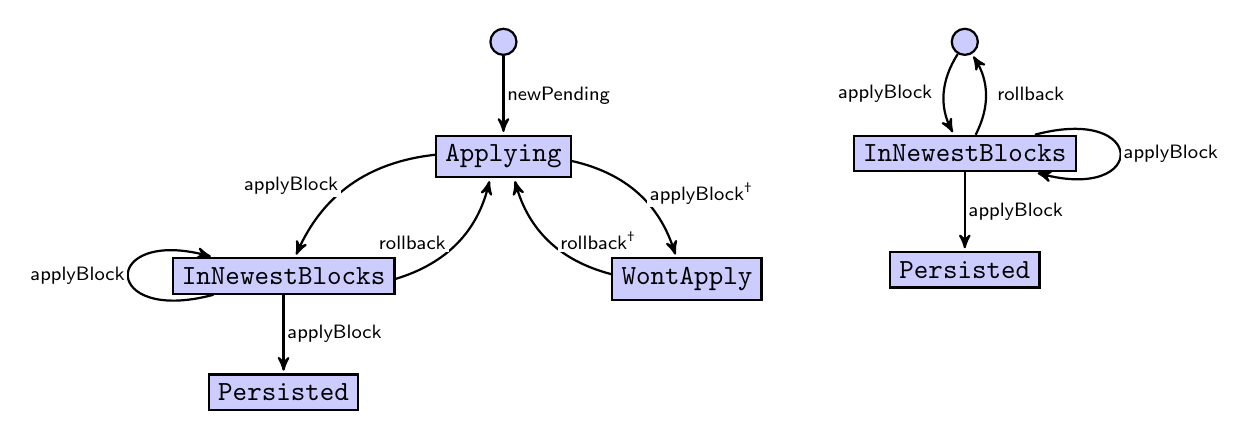
\begin{tikzpicture}[->,>=stealth',shorten >=1pt,auto,node distance=2cm,
  thick,main node/.style={rectangle,fill=blue!20,draw,minimum size=1mm}]

  \node[main node,style={circle}] (LStart) {};
  \node[main node] (LApplying)      [below=1cm of LStart] {\texttt{Applying}};
  \node[main node] (LInNewestBlock) [below left=1cm and 0.5cm of LApplying] {\texttt{InNewestBlocks}};
  \node[main node] (LWontApply)     [below right=1cm and 0.5cm of LApplying] {\texttt{WontApply}};
  \node[main node] (LPersisted)     [below =1cm of LInNewestBlock] {\texttt{Persisted}};

  \path[every node/.style={font=\sffamily\scriptsize,
      fill=white,inner sep=1pt}]
    % Right-hand-side arrows rendered from top to bottom to
    % achieve proper rendering of labels over arrows.
    (LStart)
      edge node {$\mathsf{newPending}$} (LApplying)
    (LApplying)
      edge [bend right=30] node[left=1mm] {$\mathsf{applyBlock}$} (LInNewestBlock)
      edge [bend left=30]  node[right=1mm] {$\mathsf{applyBlock}^\dagger$} (LWontApply)
    (LInNewestBlock)
      edge [loop left]     node {$\mathsf{applyBlock}$} (LInNewestBlock)
      edge [bend right=30] node[left=1mm] {$\mathsf{rollback}$} (LApplying)
      edge node {$\mathsf{applyBlock}$} (LPersisted)
    (LWontApply)
      edge [bend left=30] node[right=1mm] {$\mathsf{rollback}^\dagger$} (LApplying)
    ;

  \node[main node,style={circle}] (RStart) [right=5.5cm of LStart] {};
  \node[main node] (RInNewestBlock) [below=1cm of RStart] {\texttt{InNewestBlocks}};
  \node[main node] (RPersisted)     [below=1cm of RInNewestBlock] {\texttt{Persisted}};

  \path[every node/.style={font=\sffamily\scriptsize,
      fill=white,inner sep=1pt}]
    % Right-hand-side arrows rendered from top to bottom to
    % achieve proper rendering of labels over arrows.
    (RStart)
      edge [bend right=30] node[left=1mm] {$\mathsf{applyBlock}$} (RInNewestBlock)
    (RInNewestBlock)
      edge [loop right]     node {$\mathsf{applyBlock}$} (RInNewestBlock)
      edge [bend right=30] node[right=1mm] {$\mathsf{rollback}$} (RStart)
      edge node {$\mathsf{applyBlock}$} (RPersisted)
    ;
\end{tikzpicture}
\caption{\label{fig:transaction_state}Transaction state transitions (outgoing, \emph{left}, and incoming, \emph{right}). We will come back to the marked transitions ($\dagger$) in Section~\ref{sec:submission_interface}.}
\end{figure}

\section{Transaction Submission}
\label{sec:transaction_submission}

An actual implementation of the wallet needs to broadcast pending transactions
to the network, monitor when they get included in the blockchain, re-submit them
if they don't get included, and perhaps eventually decide to give up on them if
for some reason they do not get included.

This functionality does not need to be part of the wallet proper. In
\cref{sec:submission_interface} we will discuss the interface to this
component, and in \cref{sec:submission_implementation} we will give a
concrete simple implementation (which however still ignores any actual
networking issues).

\subsection{Interface}
\label{sec:submission_interface}

The interface to the transaction submission layer is shown in
\cref{fig:transaction_submission_layer}. It is of a similar nature as
interface to the wallet itself (\cref{fig:wallet_interface}). Just like
the wallet expects to be notified of events such as `new block arrived' and
`user submitted a new transaction', the submission layer expects to be notified
when the set of pending transactions grows or shrinks, and whenever a time slot
has passed (more on that below).

\begin{figure}
\begin{align*}
\mathsf{addPending} & :: \mathbb{P}(\mathsf{Tx}) \rightarrow \mathsf{Submission} \rightarrow \mathsf{Submission} \\
\mathsf{remPending} & :: \mathbb{P}(\mathsf{Tx}) \rightarrow \mathsf{Submission} \rightarrow \mathsf{Submission} \\
\mathsf{tick}       & :: \mathsf{Submission} \rightarrow (\mathbb{P}(\mathsf{Tx}), \mathsf{Submission})
\end{align*}
\caption{\label{fig:transaction_submission_layer}Transaction submission layer}
\end{figure}

It is the responsibility of the wallet to
%
\begin{itemize}
\item call $\mathsf{addPending}$ on $\mathsf{newPending}$ and (possibly) on $\mathsf{rollback}$
\item call $\mathsf{remPending}$ on $\mathsf{applyBlock}$ and $\mathsf{cancel}$
\end{itemize}

In addition there must be a thread that periodically calls $\mathsf{tick}$, to
give the submission layer a chance to resubmit transactions that haven't made it
into the blockchain yet. The set of transactions returned by $\mathsf{tick}$ are
the transactions that the submission layer gave up on (see below); the wallet
should remove such transactions from its $\mathit{pending}$ set. From the point
of view of the wallet model this corresponds to a new function
%
\begin{align*}
& \mathsf{cancel} :: \mathbb{P}(\mathsf{Tx}) \rightarrow \mathsf{Wallet} \rightarrow \mathsf{Wallet} \\
& \mathsf{cancel} ~ \mathit{txs} ~ (\mathit{checkpoints}, \mathit{txInfo}) = (\mathsf{map} ~ \mathsf{cancel'} ~ \mathit{checkpoints}, \mathit{txInfo}) \\
& \qquad \text{where} ~ \mathsf{cancel}' ~ (\mathit{utxo}, \mathit{pending}, \mathit{blockMeta}) = (\mathit{utxo}, \mathit{pending} \setminus \mathit{txs}, \mathit{blockMeta})
\end{align*}
%
By the logic of \cref{sec:transaction_status}, such a transaction would
be reported as $\mathtt{WontApply}$. Since we removed the transaction from the
$\mathit{pending}$ set in all checkpoints\footnote{If the overhead of traversing
all checkpoints is too large, an alternative implementation strategy would be to
maintain an explicit $\mathit{cancelled}$ set of transaction as part of the
wallet's state.}, however, a rollback won't reintroduce it into
$\mathit{pending}$; if the user wants to explicitly tell the wallet to try this
transaction again they will need to call $\mathsf{newPending}$. Effectively,
$\mathsf{cancel}$ becomes a secondary way in which a transaction may go from
$\texttt{Applying}$ to $\texttt{WontApply}$ (arrow marked $\mathsf{applyBlock}^\dagger$), and
$\mathsf{newPending}$ a secondary way to get back from $\texttt{WontApply}$ to
$\texttt{Applying}$ (arrow marked $\mathsf{rollback}^\dagger$).

\subsection{Implementation}
\label{sec:submission_implementation}

\cref{fig:submission_layer_impl} shows a simple implementation of the
submission layer.  Part of the goal of this section is to show that the
submission layer has sufficient information and does not need further support
from the core wallet layer---indeed, does not need to know it exists at all.

The state of the submission layer consists of a mirror copy of the pending set
of the wallet, as well as a schedule of which transactions to (re)submit next.
The schedule is modelled as a simple list of time slots, recording for each slot
the transactions that should be submitted, along with a submission count for
each transaction.
%
\begin{itemize}
\item When the submission layer is notified of new pending transactions,
it adds those to its $\mathit{pending}$ set and schedules them to be submitted
in the next slot, recording an initial submission count of 0.
\item When the wallet tells the submission layer that some transactions are
no longer pending (because they have been confirmed, because they have become
invalid, or for other reasons), the submission layer simply removes them
from its local $\mathit{pending}$ set.
\item The submission layer is parameterised over a `resubmission function'
$\varrho$. At the start of each time slot, the submission layer calls $\varrho$
to resubmit the set of transactions that are due, possibly dropping some
transactions that have reached a maximum submission count.
\end{itemize}

Although our model here does not deal with actual networking concerns, a
typical side-effectful implementation of $\varrho$ would
%
\begin{itemize}
\item Drop any transactions that have reached their maximum submission
count, possibly notifying the user
(note that $\varrho$ only gets called for transactions that are still listed as
pending).
\item Resubmit the remaining transactions to the network, and reschedule them
for the next attempt later. If desired, the submission count can be used to
implement exponential back-off.
\end{itemize}

The concept of time slots is essentially private to the submission layer; it
can, but does not have to, line up with the underlying blockchain slot length
(indeed, we don't need to assume that the underlying blockchain even \emph{has}
a slot length).

In principle $\mathit{pending}$ could be dropped from the submission layer; the
reason that we don't is that this would mean that $\mathsf{remPending}$ would
have to traverse the entire schedule to remove the transactions from each slot.
By keeping a separate $\mathit{pending}$ set we avoid this traversal, only
checking the pending set at the point where we need it. The wallet's
$\mathit{pending}$ set and the submission layer's one don't need to be in
perfect sync:
%
\begin{itemize}
\item If
\begin{math}
t \in    \mathit{pending}_\mathsf{Wallet} \text{ but }
t \notin \mathit{pending}_\mathsf{Submission}
\end{math},
it might mean that the wallet hasn't informed the submission layer yet of a
new transaction, and it will just be submitted a little bit later, or it might
mean that the submission layer removed a transaction from its pending set
because it's given up on it, but the wallet hasn't reacted to the notification
from the submission layer yet.\footnote{We could alternatively insist that the
submission layer doesn't remove any transactions from its pending set until
the wallet tells it so. Relaxing that restriction however allows us to state
an invariant that anything in the submission layer's pending set must also
be scheduled.}

\item If
\begin{math}
t \notin \mathit{pending}_\mathsf{Wallet} \text{ but (still) }
t \in    \mathit{pending}_\mathsf{Submission}
\end{math}
then (depending on the submission count) the submission layer may resubmit a
transaction which has already been included in the blockchain, or report the
transaction as `dropped'. The former is harmless; the latter at worst simply
confusing. Moreover,  this may happen even if the wallet and the submission
layer \emph{are} synchronised: it's entirely possible that the transaction has
been included in the blockchain but the wallet hasn't been informed of the block
yet.
\end{itemize}

Although the specification uses a simple list for its schedule, if the overhead
of a linear scan over all time slots to reschedule transactions is unacceptable,
it can of course easily use a different list-like datatype such as a
fingertree\footnote{Available in Haskell as \texttt{Data.Sequence}.}
\citep{hinze_paterson_2006}.

\begin{figure}
%
\emph{Types}
%
\begin{align*}
  \mathit{schedule}
& \in \mathsf{Schedule} = [\mathsf{Tx} \mapsto \mathbb{N}]
\end{align*}
%
\emph{Resubmission parameter}
%
\begin{align*}
  \varrho
& \in (\mathsf{Tx} \mapsto \mathbb{N}) \times \mathsf{Schedule} \rightarrow \mathbb{P}(\mathsf{Tx}) \times \mathsf{Schedule}
\end{align*}
%
\emph{State}
%
\begin{align*}
  (\mathit{pending}, \mathit{schedule})
& \in \mathsf{Submission} = \mathsf{Pending} \times \mathsf{Schedule}
\end{align*}
%
\emph{Atomic updates}
%
\begin{align*}
  \mathsf{addPending}
    ~ \mathit{txs}
    ~ (\mathit{pending}, \mathit{schedule})
& = ( \mathit{pending} \cup \mathit{txs}
    , \{ \mathit{tx} \mapsto 0 \mid \mathit{tx} \in \mathit{txs} \} : \mathit{schedule}
    )
\\
  \mathsf{remPending}
    ~ \mathit{txs}
    ~ (\mathit{pending}, \mathit{schedule})
& = ( \mathit{pending} \setminus \mathit{txs}
    , \mathit{schedule}
    )
\end{align*}
\begin{align*}
& \mathsf{tick} ~ (\mathit{pending}, []) = (\emptyset, (\mathit{pending}, [])) \\
& \mathsf{tick} ~ (\mathit{pending}, \mathit{due} : \mathit{schedule})
= (\mathit{dropped}, (\mathit{pending}, \mathit{schedule'})) \\
& \qquad\text{where~} (\mathit{dropped}, \mathit{schedule}')
= \varrho(\mathit{pending} \restrictdom \mathit{due}, \mathit{schedule})
\end{align*}
%
\caption{\label{fig:submission_layer_impl}Submission layer implementation}
\end{figure}

\subsection{Persistence}

The state of the submission layer does not need to be persisted. If the wallet
is shutdown for some period of time, the submission layer can simply be
re-initialised from the state of the wallet, starting the submission process
afresh for any transactions that the wallet still reports as pending. As long
as the submission layer is able to report `time until dropped' for still
pending transactions, so that the user can see that all pending transactions
have been reset to the initial expiry time of say 1 hour, it will be clear to
the user what happened. This should be sufficient even for exchange nodes
(especially since they will shutdown the wallet only very rarely).

If this reset to 1 hour (or whatever the expiry time is) is not acceptable,
then the state of the submission layer \emph{does} need to be persisted.
The creation time of the transactions cannot be used, since this is a static
value and will not change when the transaction gets explicitly resubmitted
by the user after the submission layer decided to drop it.

\subsection{Transactions with TTL}
\label{sec:TTL}

Dropping transactions after a certain time has passed is merely a stop-gap
measure. Once a transaction has been broadcast across the network, it may be
included at any point, possibly long after the submission layer has given up on
it (unless the chain includes confirmed transactions that spends one or more of
the transaction's inputs).

The proper solution to this problem is to introduce a time-to-live (TTL) value
for transactions, stating that the transaction must be included in the
blockchain before a certain slot and simply dropped otherwise. A proper treatment
of TTL would require revisiting every aspect of this specification; for now
we just make a few observations:

\begin{itemize}
\item Once a TTL has been introduced, the core wallet \emph{itself} can remove
transactions from its $\mathit{pending}$ set once the TTL has expired.
\item This means that the submission layer does not  need to implement expiry
anymore, although it may still wish to keep track of a submission count so that
it can implement exponential back-off.
\item Persistence for the submission layer becomes even less important.
The expiry of a transaction is now determined by the state of the blockchain,
and moreover once a transaction \emph{is} expired it cannot be resubmitted again
(a new transaction, with a new TTL, must be signed).
\end{itemize}

\section{Input selection}

In this wallet specification we assume that new transactions to be submitted are
provided to $\mathsf{newPending}$ fully formed. In reality this is preceded by a
process known as \emph{input selection} or \emph{coin selection} which, given a
set of desired outputs (that is, a \emph{payment} that the user wishes to make),
selects one or more inputs from the wallet's UTxO to cover that payment and the
transaction fee, returning any change back to the wallet. The result of input
selection is a fully formed transaction which can then be passed to
$\mathsf{newPending}$. This is summarised more formally in
\cref{fig:input_selection_sig}.

\begin{figure}[tb]
\begin{align*}
& \mathsf{selectInputs} \in \mathsf{UTxO} \to \mathbb{P}(\mathsf{TxOut}) \to \mathsf{Maybe} ~ \mathsf{Tx} \\
\\
& \mathsf{Just} ~ (\mathit{inputs}, \mathit{outputs}') = \mathsf{selectInputs} ~ \mathit{utxo} ~ \mathit{outputs} \\
& \qquad \mathbf{ensures~}
\begin{array}[t]{l@{\;}l@{\;}l}
\mathit{inputs}          & \subseteq & \dom \mathit{utxo} \\
\range ~ \mathit{outputs}' & \supseteq & \mathit{outputs}   \\
\multicolumn{3}{l}{\range ~ \mathit{outputs}' \setminus \mathit{outputs} \subseteq \mathsf{TxOut_{ours}}} \\
\end{array}
\end{align*}
\caption{\label{fig:input_selection_sig}Specification of input selection}
\end{figure}

Input selection is a large topic which merits a detailed study in its own right.
Moreover, since input selection has multiple mutually incompatible goals, there
is no single one-size-fits-all input selection algorithm. We will start with
listing some goals that an input selection algorithm may have in
Section~\ref{sec:inputselection_goals}, and some different use cases in
Section~\ref{sec:input_selection_use_cases}. The remainder of this section will
then continue by describing the algorithm we propose to use in the wallet, along
with a detailed analysis (by means of simulation) of how the algorithm performs
under various circumstances.

\subsection{Goals}
\label{sec:inputselection_goals}

In this section we list some goals that a particular input selection algorithm
may have. As is well-known \citep{lopp:challenges}, many of these goals compete
with each other. We may therefore wish to give wallet users some influence over
this process, enabling them to prioritise some goals over others.

\paragraph{Low transaction fees.}
Transactions must include a transaction fee, which is based on the size of the
transaction (\cref{app:transaction_fees}). A good input selection
algorithm will attempt to keep these transaction fees low. One complication here
is that the fee depends on the size of the transaction, but the size of
the transaction may depend on the fee since we may need to add more inputs to
the transaction in order to cover the fee. Thus fee calculation and input
selection are interdependent. There are situations where it is not immediately
obvious that there is a terminating algorithm for selecting inputs and fees
optimally. Note that minimising transaction fees \emph{over time} does not
necessarily mean that \emph{every individual} transaction will be as small as
possible.

\paragraph{Cryptographic security.}
Once an input at an address has been spent, its public key is publicly
known and is arguably no longer suitable for very long term storage of funds due
to the evolution of cryptography. The standard solution with input selection is
to add a constraint that if we pick one input then we must pick all other inputs
that were output to the same address. This results in no more funds remaining at
the address (assuming an address non-reuse strategy such that there are no later
payments to that address).

\paragraph{Privacy.}
The privacy goal is to make it impractical for other people observing the
transactions in the ledger to tie an identity to all the funds belonging to that
identity. For instance, it is preferable to have transactions with single
inputs only, since otherwise attackers can reasonably assume\footnote{In systems
such as Bitcoin there are services known as ``laundry services'', ``mixers'' or
``tumblers'' \citep{10.1007/978-3-319-70290-2_18}, which are trusted
third-parties that combine payments from various users into a single transaction, to
break this assumption.}  that of all the transactions inputs belong to the same
identity \citep{fergal}. On the output side, we may wish to take steps to ensure
that attackers cannot easily identify which output is the change output
\citep{8260674}. For instance, for single payment transactions, we could try to
ensure that the change output is roughly as large as the payment itself. Some
systems give users the ability to override input selection on a per-transaction
bases (sometimes known as ``coin control''), since some transactions are more
sensitive than others.

\paragraph{UTxO size.}
A transaction with a single input and two outputs will increase the size of the
global UTxO by one entry, and (provided one of those is a change address), leave
the size of the wallet's own UTxO unchanged; since incoming transactions will
always grow the size of the wallet's UTxO, this means with such transactions the
size of the wallet's UTxO will also grow without bound over time. Since the UTxO
is kept in memory, this is undesirable. Instead input selection should attempt
to keep the size of the UTxO steady. More specifically, if incoming transactions
grow the wallet's UTxO by $n$ entries on average, and the ratio of incoming
transactions to outgoing transactions is $r : 1$, then ideally outgoing
transactions should shrink the wallet's UTxO by $r \times n$ entries on average.

\paragraph{Distribution of magnitude of unspent outputs.}
Input selection can try to keep the distribution of the magnitude of unspent
outputs close some ideal distribution. An obvious example is to avoid ``dust'':
many tiny unspent outputs that result from change outputs. More generally,
input selection can be given an ideal distribution a priori, or keep one
dynamically based on the payment requests that come in. An example of an
a-priori known requirement would be the ability to make payments of a certain
size; if the UTxO only contains small unspent outputs, then for very large
payments the resulting transaction might exceed the maximum transaction size.
Conversely, if the UTxO only contains large outputs, the wallet may be forced to
rely on unconfirmed transactions to maintain throughput, something we've
expressly disallowed in this specification (\cref{sec:updatePending})
because it has negative consequences on networking performance.
The privacy consequences of this kind of UTxO maintenance are far from obvious,
but we note that some authors claim it may actually \emph{help}
\citep[Section 2]{10.1007/978-3-642-39884-1_2}.

\subsection{Use cases}
\label{sec:input_selection_use_cases}

As an example of how different users might prioritise different goals,
we will consider two use cases, at opposite ends of the spectrum: small end
users and exchange nodes.

\emph{Exchange nodes.}
Exchanges have high rates of incoming and outgoing transactions, large overall
balances and will tend to have large UTxOs. For this use case we are concerned
with asymptotic complexity (due to the large UTxO) and have a goal of high
throughput, but we are not overly concerned with the goals of achieving privacy
or minimising fees. Exchanges tend to follow deposit policies which are
incompatible with the cryptographic security goal as described above, so this is
not a goal of the policy. Exchanges may occasionally need to make very large
payments.

\emph{Individual users.}
For individual users we assume a low rate of incoming and outgoing transactions
and a comparatively small UTxO. For this use case we are not too concerned with
asymptotic complexity as the UTxO is assumed to be small, nor with a goal of
high throughput. We are concerned with the privacy goal, as individual users
are able to use their wallets in a way that preserves a degree of privacy. We
are somewhat concerned with keeping fees reasonably low. Users may want the
ability to `empty their wallet' (i.e., create a single transaction that
spends all of the wallet's UTxO, sending it to a single output address.)

\subsection{Self organisation}
\label{sec:selforganisation}

The term `self organisation' refers to the emergence of complex behaviour
(typically in biological systems) from simple rules and random fluctuations.
In this section we will see how we can take advantage of self organisation
to design a simple yet effective coin selection algorithm.

In this section we present the conclusions of an in-depth study of coin
selection that we have done as part of the the redesign of the Cardano wallet.
We will describe some of the problems and trade-offs that need to be made. We
then propose a novel coin selection algorithm. The algorithm is efficient and
straight-forward to implement, and through studying simulations of the algorithm
under various conditions we will see that it is very effective.
As our starting point, we will use the random algorithm described by Mark
Erhardt in his masters thesis \citep{Erhardt:thesis}.

\subsection{Dust}

An obvious strategy that many coin selection algorithms use in some form or
other is ``try to get as close to the requested value as possible''. The problem
with such an approach is that it tends to create a lot of \emph{dust}: small
unspent outputs that remain unused in the user's wallet because they're not
particularly useful. For example, consider the `largest first' algorithm: a
simple algorithm which considers all unspent outputs of the wallet in order of
size, adding them to a running total until it has covered the requested amount.

Figure~\ref{fig:inputselection:normal_3to1_largest} shows the effect of this
algorithm. In order to evaluate a coin selection policy we need an ``event
stream'' of deposits and withdrawals to evaluate it against. For the particular
simulation shown in Figure~\ref{fig:inputselection:normal_3to1_largest} we use a
3:1 ratio between deposits and withdrawals (i.e., 3 times more deposits than
withdrawals), with both deposits and withdrawals normally distributed. We will
consider many more different event streams later in this section.

\begin{figure}[p]
\begin{center}
\scriptsize
\begin{tabular}{ll}
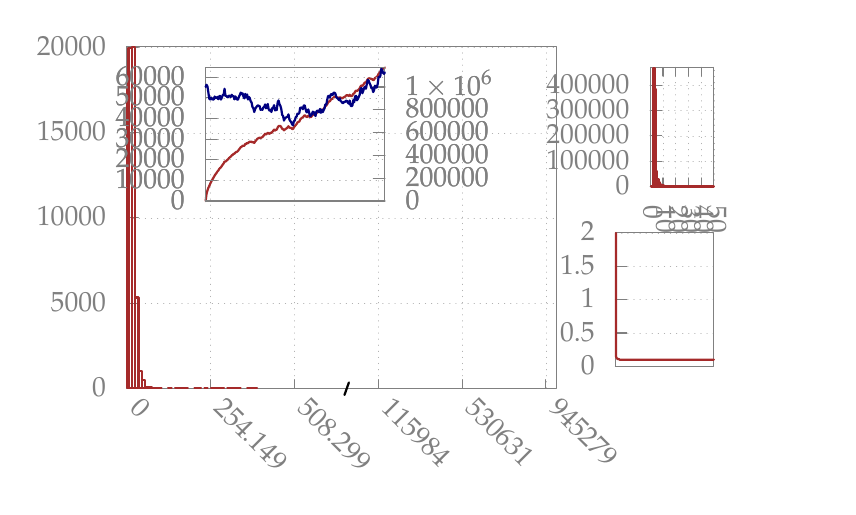
\begin{tikzpicture}[gnuplot, xscale=0.8, yscale=0.6]
%% generated with GNUPLOT 5.2p2 (Lua 5.3; terminal rev. 99, script rev. 102)
%% wo 11 jul 2018 09:42:07 CEST
\path (0.000,0.000) rectangle (12.500,8.750);
\gpcolor{color=gp lt color axes}
\gpsetlinetype{gp lt axes}
\gpsetdashtype{gp dt axes}
\gpsetlinewidth{0.50}
\draw[gp path] (1.380,1.218)--(8.197,1.218);
\gpcolor{rgb color={0.502,0.502,0.502}}
\gpsetlinetype{gp lt border}
\gpsetdashtype{gp dt solid}
\gpsetlinewidth{1.00}
\draw[gp path] (1.380,1.218)--(1.560,1.218);
\node[gp node right] at (1.196,1.218) {$0$};
\gpcolor{color=gp lt color axes}
\gpsetlinetype{gp lt axes}
\gpsetdashtype{gp dt axes}
\gpsetlinewidth{0.50}
\draw[gp path] (1.380,3.019)--(8.197,3.019);
\gpcolor{rgb color={0.502,0.502,0.502}}
\gpsetlinetype{gp lt border}
\gpsetdashtype{gp dt solid}
\gpsetlinewidth{1.00}
\draw[gp path] (1.380,3.019)--(1.560,3.019);
\node[gp node right] at (1.196,3.019) {$5000$};
\gpcolor{color=gp lt color axes}
\gpsetlinetype{gp lt axes}
\gpsetdashtype{gp dt axes}
\gpsetlinewidth{0.50}
\draw[gp path] (1.380,4.821)--(8.197,4.821);
\gpcolor{rgb color={0.502,0.502,0.502}}
\gpsetlinetype{gp lt border}
\gpsetdashtype{gp dt solid}
\gpsetlinewidth{1.00}
\draw[gp path] (1.380,4.821)--(1.560,4.821);
\node[gp node right] at (1.196,4.821) {$10000$};
\gpcolor{color=gp lt color axes}
\gpsetlinetype{gp lt axes}
\gpsetdashtype{gp dt axes}
\gpsetlinewidth{0.50}
\draw[gp path] (1.380,6.622)--(8.197,6.622);
\gpcolor{rgb color={0.502,0.502,0.502}}
\gpsetlinetype{gp lt border}
\gpsetdashtype{gp dt solid}
\gpsetlinewidth{1.00}
\draw[gp path] (1.380,6.622)--(1.560,6.622);
\node[gp node right] at (1.196,6.622) {$15000$};
\gpcolor{color=gp lt color axes}
\gpsetlinetype{gp lt axes}
\gpsetdashtype{gp dt axes}
\gpsetlinewidth{0.50}
\draw[gp path] (1.380,8.423)--(8.197,8.423);
\gpcolor{rgb color={0.502,0.502,0.502}}
\gpsetlinetype{gp lt border}
\gpsetdashtype{gp dt solid}
\gpsetlinewidth{1.00}
\draw[gp path] (1.380,8.423)--(1.560,8.423);
\node[gp node right] at (1.196,8.423) {$20000$};
\gpcolor{color=gp lt color axes}
\gpsetlinetype{gp lt axes}
\gpsetdashtype{gp dt axes}
\gpsetlinewidth{0.50}
\draw[gp path] (1.380,1.218)--(1.380,8.441);
\gpcolor{rgb color={0.502,0.502,0.502}}
\gpsetlinetype{gp lt border}
\gpsetdashtype{gp dt solid}
\gpsetlinewidth{1.00}
\draw[gp path] (1.380,1.218)--(1.380,1.398);
\node[gp node left,rotate=-45] at (1.380,1.034) {$0$};
\gpcolor{color=gp lt color axes}
\gpsetlinetype{gp lt axes}
\gpsetdashtype{gp dt axes}
\gpsetlinewidth{0.50}
\draw[gp path] (2.710,1.218)--(2.710,8.441);
\gpcolor{rgb color={0.502,0.502,0.502}}
\gpsetlinetype{gp lt border}
\gpsetdashtype{gp dt solid}
\gpsetlinewidth{1.00}
\draw[gp path] (2.710,1.218)--(2.710,1.398);
\node[gp node left,rotate=-45] at (2.710,1.034) {$254.149$};
\gpcolor{color=gp lt color axes}
\gpsetlinetype{gp lt axes}
\gpsetdashtype{gp dt axes}
\gpsetlinewidth{0.50}
\draw[gp path] (4.040,1.218)--(4.040,8.441);
\gpcolor{rgb color={0.502,0.502,0.502}}
\gpsetlinetype{gp lt border}
\gpsetdashtype{gp dt solid}
\gpsetlinewidth{1.00}
\draw[gp path] (4.040,1.218)--(4.040,1.398);
\node[gp node left,rotate=-45] at (4.040,1.034) {$508.299$};
\gpcolor{color=gp lt color axes}
\gpsetlinetype{gp lt axes}
\gpsetdashtype{gp dt axes}
\gpsetlinewidth{0.50}
\draw[gp path] (5.370,1.218)--(5.370,8.441);
\gpcolor{rgb color={0.502,0.502,0.502}}
\gpsetlinetype{gp lt border}
\gpsetdashtype{gp dt solid}
\gpsetlinewidth{1.00}
\draw[gp path] (5.370,1.218)--(5.370,1.398);
\node[gp node left,rotate=-45] at (5.370,1.034) {$115984$};
\gpcolor{color=gp lt color axes}
\gpsetlinetype{gp lt axes}
\gpsetdashtype{gp dt axes}
\gpsetlinewidth{0.50}
\draw[gp path] (6.701,1.218)--(6.701,8.441);
\gpcolor{rgb color={0.502,0.502,0.502}}
\gpsetlinetype{gp lt border}
\gpsetdashtype{gp dt solid}
\gpsetlinewidth{1.00}
\draw[gp path] (6.701,1.218)--(6.701,1.398);
\node[gp node left,rotate=-45] at (6.701,1.034) {$530631$};
\gpcolor{color=gp lt color axes}
\gpsetlinetype{gp lt axes}
\gpsetdashtype{gp dt axes}
\gpsetlinewidth{0.50}
\draw[gp path] (8.031,1.218)--(8.031,8.441);
\gpcolor{rgb color={0.502,0.502,0.502}}
\gpsetlinetype{gp lt border}
\gpsetdashtype{gp dt solid}
\gpsetlinewidth{1.00}
\draw[gp path] (8.031,1.218)--(8.031,1.398);
\node[gp node left,rotate=-45] at (8.031,1.034) {$945279$};
\draw[gp path] (1.380,8.441)--(1.380,1.218)--(8.197,1.218)--(8.197,8.441)--cycle;
\gpcolor{rgb color={0.647,0.165,0.165}}
\gpsetlinewidth{2.00}
\draw[gp path] (1.380,1.218)--(1.380,7.579)--(1.406,7.579)--(1.406,1.218)--cycle;
\draw[gp path] (1.406,1.218)--(1.406,8.416)--(1.459,8.416)--(1.459,1.218)--cycle;
\draw[gp path] (1.459,1.218)--(1.459,8.441)--(1.511,8.441)--(1.511,1.218)--cycle;
\draw[gp path] (1.511,1.218)--(1.511,3.136)--(1.563,3.136)--(1.563,1.218)--cycle;
\draw[gp path] (1.563,1.218)--(1.563,1.583)--(1.616,1.583)--(1.616,1.218)--cycle;
\draw[gp path] (1.616,1.218)--(1.616,1.395)--(1.668,1.395)--(1.668,1.218)--cycle;
\draw[gp path] (1.668,1.218)--(1.668,1.243)--(1.720,1.243)--(1.720,1.218)--cycle;
\draw[gp path] (1.720,1.218)--(1.720,1.238)--(1.773,1.238)--(1.773,1.218)--cycle;
\draw[gp path] (1.773,1.218)--(1.773,1.224)--(1.825,1.224)--(1.825,1.218)--cycle;
\draw[gp path] (1.825,1.218)--(1.825,1.219)--(1.877,1.219)--(1.877,1.218)--cycle;
\draw[gp path] (1.877,1.218)--(1.930,1.218)--cycle;
\draw[gp path] (2.034,1.218)--(2.034,1.219)--(2.087,1.219)--(2.087,1.218)--cycle;
\draw[gp path] (2.139,1.218)--(2.139,1.219)--(2.191,1.219)--(2.191,1.218)--cycle;
\draw[gp path] (2.191,1.218)--(2.244,1.218)--cycle;
\draw[gp path] (2.244,1.218)--(2.244,1.219)--(2.296,1.219)--(2.296,1.218)--cycle;
\draw[gp path] (2.296,1.218)--(2.348,1.218)--cycle;
\draw[gp path] (2.453,1.218)--(2.505,1.218)--cycle;
\draw[gp path] (2.505,1.218)--(2.558,1.218)--cycle;
\draw[gp path] (2.610,1.218)--(2.662,1.218)--cycle;
\draw[gp path] (2.715,1.218)--(2.767,1.218)--cycle;
\draw[gp path] (2.767,1.218)--(2.767,1.219)--(2.819,1.219)--(2.819,1.218)--cycle;
\draw[gp path] (2.819,1.218)--(2.872,1.218)--cycle;
\draw[gp path] (2.872,1.218)--(2.924,1.218)--cycle;
\draw[gp path] (2.976,1.218)--(2.976,1.219)--(3.029,1.219)--(3.029,1.218)--cycle;
\draw[gp path] (3.029,1.218)--(3.029,1.219)--(3.081,1.219)--(3.081,1.218)--cycle;
\draw[gp path] (3.081,1.218)--(3.133,1.218)--cycle;
\draw[gp path] (3.133,1.218)--(3.186,1.218)--cycle;
\draw[gp path] (3.290,1.218)--(3.343,1.218)--cycle;
\draw[gp path] (3.343,1.218)--(3.343,1.219)--(3.395,1.219)--(3.395,1.218)--cycle;
\draw[gp path] (3.395,1.218)--(3.447,1.218)--cycle;
\gpcolor{color=gp lt color border}
\draw[gp path](4.834,1.074)--(4.904,1.337);
%% coordinates of the plot area
\gpdefrectangularnode{gp plot 1}{\pgfpoint{1.380cm}{1.218cm}}{\pgfpoint{8.197cm}{8.441cm}}
\gpcolor{color=gp lt color axes}
\gpsetlinetype{gp lt axes}
\gpsetdashtype{gp dt axes}
\gpsetlinewidth{0.50}
\draw[gp path] (2.630,5.180)--(5.475,5.180);
\gpcolor{rgb color={0.502,0.502,0.502}}
\gpsetlinetype{gp lt border}
\gpsetdashtype{gp dt solid}
\gpsetlinewidth{1.00}
\draw[gp path] (2.630,5.180)--(2.810,5.180);
\node[gp node right] at (2.446,5.180) {$0$};
\gpcolor{color=gp lt color axes}
\gpsetlinetype{gp lt axes}
\gpsetdashtype{gp dt axes}
\gpsetlinewidth{0.50}
\draw[gp path] (2.630,5.616)--(5.475,5.616);
\gpcolor{rgb color={0.502,0.502,0.502}}
\gpsetlinetype{gp lt border}
\gpsetdashtype{gp dt solid}
\gpsetlinewidth{1.00}
\draw[gp path] (2.630,5.616)--(2.810,5.616);
\node[gp node right] at (2.446,5.616) {$10000$};
\gpcolor{color=gp lt color axes}
\gpsetlinetype{gp lt axes}
\gpsetdashtype{gp dt axes}
\gpsetlinewidth{0.50}
\draw[gp path] (2.630,6.053)--(5.475,6.053);
\gpcolor{rgb color={0.502,0.502,0.502}}
\gpsetlinetype{gp lt border}
\gpsetdashtype{gp dt solid}
\gpsetlinewidth{1.00}
\draw[gp path] (2.630,6.053)--(2.810,6.053);
\node[gp node right] at (2.446,6.053) {$20000$};
\gpcolor{color=gp lt color axes}
\gpsetlinetype{gp lt axes}
\gpsetdashtype{gp dt axes}
\gpsetlinewidth{0.50}
\draw[gp path] (2.630,6.490)--(5.475,6.490);
\gpcolor{rgb color={0.502,0.502,0.502}}
\gpsetlinetype{gp lt border}
\gpsetdashtype{gp dt solid}
\gpsetlinewidth{1.00}
\draw[gp path] (2.630,6.490)--(2.810,6.490);
\node[gp node right] at (2.446,6.490) {$30000$};
\gpcolor{color=gp lt color axes}
\gpsetlinetype{gp lt axes}
\gpsetdashtype{gp dt axes}
\gpsetlinewidth{0.50}
\draw[gp path] (2.630,6.926)--(5.475,6.926);
\gpcolor{rgb color={0.502,0.502,0.502}}
\gpsetlinetype{gp lt border}
\gpsetdashtype{gp dt solid}
\gpsetlinewidth{1.00}
\draw[gp path] (2.630,6.926)--(2.810,6.926);
\node[gp node right] at (2.446,6.926) {$40000$};
\gpcolor{color=gp lt color axes}
\gpsetlinetype{gp lt axes}
\gpsetdashtype{gp dt axes}
\gpsetlinewidth{0.50}
\draw[gp path] (2.630,7.363)--(5.475,7.363);
\gpcolor{rgb color={0.502,0.502,0.502}}
\gpsetlinetype{gp lt border}
\gpsetdashtype{gp dt solid}
\gpsetlinewidth{1.00}
\draw[gp path] (2.630,7.363)--(2.810,7.363);
\node[gp node right] at (2.446,7.363) {$50000$};
\gpcolor{color=gp lt color axes}
\gpsetlinetype{gp lt axes}
\gpsetdashtype{gp dt axes}
\gpsetlinewidth{0.50}
\draw[gp path] (2.630,7.799)--(5.475,7.799);
\gpcolor{rgb color={0.502,0.502,0.502}}
\gpsetlinetype{gp lt border}
\gpsetdashtype{gp dt solid}
\gpsetlinewidth{1.00}
\draw[gp path] (2.630,7.799)--(2.810,7.799);
\node[gp node right] at (2.446,7.799) {$60000$};
\draw[gp path] (5.475,5.180)--(5.295,5.180);
\node[gp node left] at (5.659,5.180) {$0$};
\draw[gp path] (5.475,5.663)--(5.295,5.663);
\node[gp node left] at (5.659,5.663) {$200000$};
\draw[gp path] (5.475,6.145)--(5.295,6.145);
\node[gp node left] at (5.659,6.145) {$400000$};
\draw[gp path] (5.475,6.628)--(5.295,6.628);
\node[gp node left] at (5.659,6.628) {$600000$};
\draw[gp path] (5.475,7.110)--(5.295,7.110);
\node[gp node left] at (5.659,7.110) {$800000$};
\draw[gp path] (5.475,7.593)--(5.295,7.593);
\node[gp node left] at (5.659,7.593) {$1\times10^{6}$};
\draw[gp path] (2.630,8.004)--(2.630,5.180)--(5.475,5.180)--(5.475,8.004)--cycle;
\gpcolor{rgb color={0.647,0.165,0.165}}
\gpsetlinewidth{2.00}
\draw[gp path] (2.630,5.180)--(2.644,5.327)--(2.659,5.404)--(2.673,5.457)--(2.687,5.498)%
  --(2.701,5.539)--(2.716,5.582)--(2.730,5.617)--(2.744,5.651)--(2.759,5.683)--(2.773,5.718)%
  --(2.787,5.745)--(2.802,5.771)--(2.816,5.802)--(2.830,5.821)--(2.844,5.854)--(2.859,5.878)%
  --(2.873,5.892)--(2.887,5.921)--(2.902,5.952)--(2.916,5.974)--(2.930,6.015)--(2.945,6.012)%
  --(2.959,6.031)--(2.973,6.046)--(2.987,6.064)--(3.002,6.090)--(3.016,6.105)--(3.030,6.119)%
  --(3.045,6.147)--(3.059,6.156)--(3.073,6.178)--(3.087,6.180)--(3.102,6.203)--(3.116,6.218)%
  --(3.130,6.222)--(3.145,6.242)--(3.159,6.270)--(3.173,6.291)--(3.188,6.320)--(3.202,6.328)%
  --(3.216,6.349)--(3.230,6.348)--(3.245,6.349)--(3.259,6.387)--(3.273,6.386)--(3.288,6.410)%
  --(3.302,6.399)--(3.316,6.424)--(3.331,6.436)--(3.345,6.429)--(3.359,6.436)--(3.373,6.419)%
  --(3.388,6.425)--(3.402,6.408)--(3.416,6.439)--(3.431,6.463)--(3.445,6.485)--(3.459,6.504)%
  --(3.473,6.512)--(3.488,6.523)--(3.502,6.508)--(3.516,6.523)--(3.531,6.530)--(3.545,6.555)%
  --(3.559,6.575)--(3.574,6.601)--(3.588,6.586)--(3.602,6.603)--(3.616,6.623)--(3.631,6.609)%
  --(3.645,6.601)--(3.659,6.624)--(3.674,6.621)--(3.688,6.642)--(3.702,6.664)--(3.717,6.691)%
  --(3.731,6.670)--(3.745,6.688)--(3.759,6.689)--(3.774,6.737)--(3.788,6.765)--(3.802,6.766)%
  --(3.817,6.767)--(3.831,6.743)--(3.845,6.706)--(3.859,6.702)--(3.874,6.676)--(3.888,6.691)%
  --(3.902,6.706)--(3.917,6.717)--(3.931,6.736)--(3.945,6.762)--(3.960,6.730)--(3.974,6.731)%
  --(3.988,6.725)--(4.002,6.705)--(4.017,6.702)--(4.031,6.740)--(4.045,6.761)--(4.060,6.788)%
  --(4.074,6.808)--(4.088,6.841)--(4.103,6.854)--(4.117,6.861)--(4.131,6.903)--(4.145,6.924)%
  --(4.160,6.941)--(4.174,6.948)--(4.188,6.977)--(4.203,6.994)--(4.217,6.975)--(4.231,6.962)%
  --(4.246,6.955)--(4.260,6.987)--(4.274,6.979)--(4.288,6.957)--(4.303,6.956)--(4.317,6.981)%
  --(4.331,7.004)--(4.346,7.017)--(4.360,7.001)--(4.374,7.007)--(4.388,7.038)--(4.403,7.059)%
  --(4.417,7.074)--(4.431,7.065)--(4.446,7.094)--(4.460,7.084)--(4.474,7.112)--(4.489,7.104)%
  --(4.503,7.129)--(4.517,7.153)--(4.531,7.187)--(4.546,7.201)--(4.560,7.230)--(4.574,7.266)%
  --(4.589,7.286)--(4.603,7.292)--(4.617,7.325)--(4.632,7.337)--(4.646,7.345)--(4.660,7.369)%
  --(4.674,7.385)--(4.689,7.394)--(4.703,7.373)--(4.717,7.369)--(4.732,7.371)--(4.746,7.357)%
  --(4.760,7.374)--(4.774,7.367)--(4.789,7.358)--(4.803,7.355)--(4.817,7.371)--(4.832,7.380)%
  --(4.846,7.389)--(4.860,7.412)--(4.875,7.423)--(4.889,7.412)--(4.903,7.400)--(4.917,7.428)%
  --(4.932,7.401)--(4.946,7.399)--(4.960,7.414)--(4.975,7.451)--(4.989,7.458)--(5.003,7.494)%
  --(5.018,7.518)--(5.032,7.505)--(5.046,7.520)--(5.060,7.539)--(5.075,7.562)--(5.089,7.603)%
  --(5.103,7.626)--(5.118,7.616)--(5.132,7.634)--(5.146,7.667)--(5.160,7.689)--(5.175,7.692)%
  --(5.189,7.721)--(5.203,7.758)--(5.218,7.774)--(5.232,7.777)--(5.246,7.777)--(5.261,7.757)%
  --(5.275,7.761)--(5.289,7.735)--(5.303,7.746)--(5.318,7.783)--(5.332,7.791)--(5.346,7.805)%
  --(5.361,7.828)--(5.375,7.871)--(5.389,7.892)--(5.404,7.917)--(5.418,7.963)--(5.432,7.975)%
  --(5.446,7.981)--(5.461,7.983)--(5.475,8.004);
%% coordinates of the plot area
\gpdefrectangularnode{gp plot 2}{\pgfpoint{2.630cm}{5.180cm}}{\pgfpoint{5.475cm}{8.004cm}}
\gpcolor{color=gp lt color axes}
\gpsetlinetype{gp lt axes}
\gpsetdashtype{gp dt axes}
\gpsetlinewidth{0.50}
\draw[gp path] (2.630,5.180)--(5.475,5.180);
\gpcolor{rgb color={0.502,0.502,0.502}}
\gpsetlinetype{gp lt border}
\gpsetdashtype{gp dt solid}
\gpsetlinewidth{1.00}
\draw[gp path] (2.630,5.180)--(2.810,5.180);
\node[gp node right] at (2.446,5.180) {$0$};
\gpcolor{color=gp lt color axes}
\gpsetlinetype{gp lt axes}
\gpsetdashtype{gp dt axes}
\gpsetlinewidth{0.50}
\draw[gp path] (2.630,5.616)--(5.475,5.616);
\gpcolor{rgb color={0.502,0.502,0.502}}
\gpsetlinetype{gp lt border}
\gpsetdashtype{gp dt solid}
\gpsetlinewidth{1.00}
\draw[gp path] (2.630,5.616)--(2.810,5.616);
\node[gp node right] at (2.446,5.616) {$10000$};
\gpcolor{color=gp lt color axes}
\gpsetlinetype{gp lt axes}
\gpsetdashtype{gp dt axes}
\gpsetlinewidth{0.50}
\draw[gp path] (2.630,6.053)--(5.475,6.053);
\gpcolor{rgb color={0.502,0.502,0.502}}
\gpsetlinetype{gp lt border}
\gpsetdashtype{gp dt solid}
\gpsetlinewidth{1.00}
\draw[gp path] (2.630,6.053)--(2.810,6.053);
\node[gp node right] at (2.446,6.053) {$20000$};
\gpcolor{color=gp lt color axes}
\gpsetlinetype{gp lt axes}
\gpsetdashtype{gp dt axes}
\gpsetlinewidth{0.50}
\draw[gp path] (2.630,6.490)--(5.475,6.490);
\gpcolor{rgb color={0.502,0.502,0.502}}
\gpsetlinetype{gp lt border}
\gpsetdashtype{gp dt solid}
\gpsetlinewidth{1.00}
\draw[gp path] (2.630,6.490)--(2.810,6.490);
\node[gp node right] at (2.446,6.490) {$30000$};
\gpcolor{color=gp lt color axes}
\gpsetlinetype{gp lt axes}
\gpsetdashtype{gp dt axes}
\gpsetlinewidth{0.50}
\draw[gp path] (2.630,6.926)--(5.475,6.926);
\gpcolor{rgb color={0.502,0.502,0.502}}
\gpsetlinetype{gp lt border}
\gpsetdashtype{gp dt solid}
\gpsetlinewidth{1.00}
\draw[gp path] (2.630,6.926)--(2.810,6.926);
\node[gp node right] at (2.446,6.926) {$40000$};
\gpcolor{color=gp lt color axes}
\gpsetlinetype{gp lt axes}
\gpsetdashtype{gp dt axes}
\gpsetlinewidth{0.50}
\draw[gp path] (2.630,7.363)--(5.475,7.363);
\gpcolor{rgb color={0.502,0.502,0.502}}
\gpsetlinetype{gp lt border}
\gpsetdashtype{gp dt solid}
\gpsetlinewidth{1.00}
\draw[gp path] (2.630,7.363)--(2.810,7.363);
\node[gp node right] at (2.446,7.363) {$50000$};
\gpcolor{color=gp lt color axes}
\gpsetlinetype{gp lt axes}
\gpsetdashtype{gp dt axes}
\gpsetlinewidth{0.50}
\draw[gp path] (2.630,7.799)--(5.475,7.799);
\gpcolor{rgb color={0.502,0.502,0.502}}
\gpsetlinetype{gp lt border}
\gpsetdashtype{gp dt solid}
\gpsetlinewidth{1.00}
\draw[gp path] (2.630,7.799)--(2.810,7.799);
\node[gp node right] at (2.446,7.799) {$60000$};
\draw[gp path] (5.475,5.180)--(5.295,5.180);
\node[gp node left] at (5.659,5.180) {$0$};
\draw[gp path] (5.475,5.663)--(5.295,5.663);
\node[gp node left] at (5.659,5.663) {$200000$};
\draw[gp path] (5.475,6.145)--(5.295,6.145);
\node[gp node left] at (5.659,6.145) {$400000$};
\draw[gp path] (5.475,6.628)--(5.295,6.628);
\node[gp node left] at (5.659,6.628) {$600000$};
\draw[gp path] (5.475,7.110)--(5.295,7.110);
\node[gp node left] at (5.659,7.110) {$800000$};
\draw[gp path] (5.475,7.593)--(5.295,7.593);
\node[gp node left] at (5.659,7.593) {$1\times10^{6}$};
\draw[gp path] (2.630,8.004)--(2.630,5.180)--(5.475,5.180)--(5.475,8.004)--cycle;
\gpcolor{rgb color={0.000,0.000,0.502}}
\gpsetlinewidth{2.00}
\draw[gp path] (2.630,7.594)--(2.644,7.639)--(2.659,7.605)--(2.673,7.479)--(2.687,7.346)%
  --(2.701,7.329)--(2.716,7.369)--(2.730,7.334)--(2.744,7.329)--(2.759,7.327)--(2.773,7.390)%
  --(2.787,7.363)--(2.802,7.357)--(2.816,7.383)--(2.830,7.333)--(2.844,7.396)--(2.859,7.402)%
  --(2.873,7.325)--(2.887,7.368)--(2.902,7.421)--(2.916,7.429)--(2.930,7.555)--(2.945,7.403)%
  --(2.959,7.406)--(2.973,7.380)--(2.987,7.373)--(3.002,7.410)--(3.016,7.399)--(3.030,7.383)%
  --(3.045,7.427)--(3.059,7.393)--(3.073,7.399)--(3.087,7.330)--(3.102,7.393)--(3.116,7.361)%
  --(3.130,7.324)--(3.145,7.327)--(3.159,7.389)--(3.173,7.423)--(3.188,7.474)--(3.202,7.443)%
  --(3.216,7.459)--(3.230,7.388)--(3.245,7.351)--(3.259,7.447)--(3.273,7.375)--(3.288,7.433)%
  --(3.302,7.328)--(3.316,7.382)--(3.331,7.357)--(3.345,7.289)--(3.359,7.266)--(3.373,7.172)%
  --(3.388,7.143)--(3.402,7.063)--(3.416,7.125)--(3.431,7.162)--(3.445,7.184)--(3.459,7.206)%
  --(3.473,7.191)--(3.488,7.187)--(3.502,7.109)--(3.516,7.124)--(3.531,7.107)--(3.545,7.158)%
  --(3.559,7.172)--(3.574,7.222)--(3.588,7.143)--(3.602,7.162)--(3.616,7.233)--(3.631,7.118)%
  --(3.645,7.092)--(3.659,7.112)--(3.674,7.063)--(3.688,7.148)--(3.702,7.149)--(3.717,7.208)%
  --(3.731,7.097)--(3.745,7.112)--(3.759,7.105)--(3.774,7.272)--(3.788,7.307)--(3.802,7.233)%
  --(3.817,7.193)--(3.831,7.124)--(3.845,7.001)--(3.859,6.980)--(3.874,6.882)--(3.888,6.930)%
  --(3.902,6.942)--(3.917,6.957)--(3.931,6.962)--(3.945,7.013)--(3.960,6.904)--(3.974,6.873)%
  --(3.988,6.848)--(4.002,6.804)--(4.017,6.779)--(4.031,6.870)--(4.045,6.881)--(4.060,6.956)%
  --(4.074,6.965)--(4.088,7.030)--(4.103,7.022)--(4.117,7.042)--(4.131,7.154)--(4.145,7.154)%
  --(4.160,7.159)--(4.174,7.121)--(4.188,7.202)--(4.203,7.202)--(4.217,7.124)--(4.231,7.059)%
  --(4.246,7.059)--(4.260,7.118)--(4.274,7.046)--(4.288,6.974)--(4.303,6.989)--(4.317,7.017)%
  --(4.331,7.068)--(4.346,7.060)--(4.360,7.015)--(4.374,6.978)--(4.388,7.070)--(4.403,7.091)%
  --(4.417,7.090)--(4.431,7.056)--(4.446,7.129)--(4.460,7.046)--(4.474,7.111)--(4.489,7.061)%
  --(4.503,7.100)--(4.517,7.142)--(4.531,7.226)--(4.546,7.222)--(4.560,7.322)--(4.574,7.401)%
  --(4.589,7.405)--(4.603,7.366)--(4.617,7.437)--(4.632,7.440)--(4.646,7.424)--(4.660,7.467)%
  --(4.674,7.474)--(4.689,7.454)--(4.703,7.385)--(4.717,7.360)--(4.732,7.344)--(4.746,7.315)%
  --(4.760,7.353)--(4.774,7.291)--(4.789,7.281)--(4.803,7.251)--(4.817,7.256)--(4.832,7.284)%
  --(4.846,7.275)--(4.860,7.305)--(4.875,7.295)--(4.889,7.258)--(4.903,7.239)--(4.917,7.305)%
  --(4.932,7.200)--(4.946,7.183)--(4.960,7.203)--(4.975,7.317)--(4.989,7.271)--(5.003,7.396)%
  --(5.018,7.404)--(5.032,7.311)--(5.046,7.338)--(5.060,7.381)--(5.075,7.426)--(5.089,7.549)%
  --(5.103,7.569)--(5.118,7.460)--(5.132,7.511)--(5.146,7.571)--(5.160,7.596)--(5.175,7.555)%
  --(5.189,7.657)--(5.203,7.739)--(5.218,7.727)--(5.232,7.675)--(5.246,7.636)--(5.261,7.569)%
  --(5.275,7.577)--(5.289,7.485)--(5.303,7.521)--(5.318,7.620)--(5.332,7.582)--(5.346,7.579)%
  --(5.361,7.654)--(5.375,7.801)--(5.389,7.794)--(5.404,7.833)--(5.418,7.976)--(5.432,7.958)%
  --(5.446,7.893)--(5.461,7.870)--(5.475,7.901);
\gpcolor{color=gp lt color axes}
\gpsetlinetype{gp lt axes}
\gpsetdashtype{gp dt axes}
\gpsetlinewidth{0.50}
\draw[gp path] (9.688,5.488)--(10.697,5.488);
\gpcolor{rgb color={0.502,0.502,0.502}}
\gpsetlinetype{gp lt border}
\gpsetdashtype{gp dt solid}
\gpsetlinewidth{1.00}
\draw[gp path] (9.688,5.488)--(9.868,5.488);
\node[gp node right] at (9.504,5.488) {$0$};
\gpcolor{color=gp lt color axes}
\gpsetlinetype{gp lt axes}
\gpsetdashtype{gp dt axes}
\gpsetlinewidth{0.50}
\draw[gp path] (9.688,6.023)--(10.697,6.023);
\gpcolor{rgb color={0.502,0.502,0.502}}
\gpsetlinetype{gp lt border}
\gpsetdashtype{gp dt solid}
\gpsetlinewidth{1.00}
\draw[gp path] (9.688,6.023)--(9.868,6.023);
\node[gp node right] at (9.504,6.023) {$100000$};
\gpcolor{color=gp lt color axes}
\gpsetlinetype{gp lt axes}
\gpsetdashtype{gp dt axes}
\gpsetlinewidth{0.50}
\draw[gp path] (9.688,6.557)--(10.697,6.557);
\gpcolor{rgb color={0.502,0.502,0.502}}
\gpsetlinetype{gp lt border}
\gpsetdashtype{gp dt solid}
\gpsetlinewidth{1.00}
\draw[gp path] (9.688,6.557)--(9.868,6.557);
\node[gp node right] at (9.504,6.557) {$200000$};
\gpcolor{color=gp lt color axes}
\gpsetlinetype{gp lt axes}
\gpsetdashtype{gp dt axes}
\gpsetlinewidth{0.50}
\draw[gp path] (9.688,7.092)--(10.697,7.092);
\gpcolor{rgb color={0.502,0.502,0.502}}
\gpsetlinetype{gp lt border}
\gpsetdashtype{gp dt solid}
\gpsetlinewidth{1.00}
\draw[gp path] (9.688,7.092)--(9.868,7.092);
\node[gp node right] at (9.504,7.092) {$300000$};
\gpcolor{color=gp lt color axes}
\gpsetlinetype{gp lt axes}
\gpsetdashtype{gp dt axes}
\gpsetlinewidth{0.50}
\draw[gp path] (9.688,7.626)--(10.697,7.626);
\gpcolor{rgb color={0.502,0.502,0.502}}
\gpsetlinetype{gp lt border}
\gpsetdashtype{gp dt solid}
\gpsetlinewidth{1.00}
\draw[gp path] (9.688,7.626)--(9.868,7.626);
\node[gp node right] at (9.504,7.626) {$400000$};
\gpcolor{color=gp lt color axes}
\gpsetlinetype{gp lt axes}
\gpsetdashtype{gp dt axes}
\gpsetlinewidth{0.50}
\draw[gp path] (9.688,5.488)--(9.688,7.824)--(9.688,8.004);
\gpcolor{rgb color={0.502,0.502,0.502}}
\gpsetlinetype{gp lt border}
\gpsetdashtype{gp dt solid}
\gpsetlinewidth{1.00}
\draw[gp path] (9.688,5.488)--(9.688,5.668);
\draw[gp path] (9.688,8.004)--(9.688,7.824);
\node[gp node left,rotate=-90] at (9.688,5.304) {$0$};
\gpcolor{color=gp lt color axes}
\gpsetlinetype{gp lt axes}
\gpsetdashtype{gp dt axes}
\gpsetlinewidth{0.50}
\draw[gp path] (9.890,5.488)--(9.890,7.824)--(9.890,8.004);
\gpcolor{rgb color={0.502,0.502,0.502}}
\gpsetlinetype{gp lt border}
\gpsetdashtype{gp dt solid}
\gpsetlinewidth{1.00}
\draw[gp path] (9.890,5.488)--(9.890,5.668);
\draw[gp path] (9.890,8.004)--(9.890,7.824);
\node[gp node left,rotate=-90] at (9.890,5.304) {$10$};
\gpcolor{color=gp lt color axes}
\gpsetlinetype{gp lt axes}
\gpsetdashtype{gp dt axes}
\gpsetlinewidth{0.50}
\draw[gp path] (10.092,5.488)--(10.092,7.824)--(10.092,8.004);
\gpcolor{rgb color={0.502,0.502,0.502}}
\gpsetlinetype{gp lt border}
\gpsetdashtype{gp dt solid}
\gpsetlinewidth{1.00}
\draw[gp path] (10.092,5.488)--(10.092,5.668);
\draw[gp path] (10.092,8.004)--(10.092,7.824);
\node[gp node left,rotate=-90] at (10.092,5.304) {$20$};
\gpcolor{color=gp lt color axes}
\gpsetlinetype{gp lt axes}
\gpsetdashtype{gp dt axes}
\gpsetlinewidth{0.50}
\draw[gp path] (10.293,5.488)--(10.293,7.824)--(10.293,8.004);
\gpcolor{rgb color={0.502,0.502,0.502}}
\gpsetlinetype{gp lt border}
\gpsetdashtype{gp dt solid}
\gpsetlinewidth{1.00}
\draw[gp path] (10.293,5.488)--(10.293,5.668);
\draw[gp path] (10.293,8.004)--(10.293,7.824);
\node[gp node left,rotate=-90] at (10.293,5.304) {$30$};
\gpcolor{color=gp lt color axes}
\gpsetlinetype{gp lt axes}
\gpsetdashtype{gp dt axes}
\gpsetlinewidth{0.50}
\draw[gp path] (10.495,5.488)--(10.495,7.824)--(10.495,8.004);
\gpcolor{rgb color={0.502,0.502,0.502}}
\gpsetlinetype{gp lt border}
\gpsetdashtype{gp dt solid}
\gpsetlinewidth{1.00}
\draw[gp path] (10.495,5.488)--(10.495,5.668);
\draw[gp path] (10.495,8.004)--(10.495,7.824);
\node[gp node left,rotate=-90] at (10.495,5.304) {$40$};
\gpcolor{color=gp lt color axes}
\gpsetlinetype{gp lt axes}
\gpsetdashtype{gp dt axes}
\gpsetlinewidth{0.50}
\draw[gp path] (10.697,5.488)--(10.697,8.004);
\gpcolor{rgb color={0.502,0.502,0.502}}
\gpsetlinetype{gp lt border}
\gpsetdashtype{gp dt solid}
\gpsetlinewidth{1.00}
\draw[gp path] (10.697,5.488)--(10.697,5.668);
\draw[gp path] (10.697,8.004)--(10.697,7.824);
\node[gp node left,rotate=-90] at (10.697,5.304) {$50$};
\draw[gp path] (9.688,8.004)--(9.688,5.488)--(10.697,5.488)--(10.697,8.004)--cycle;
\gpfill{rgb color={0.647,0.165,0.165}} (9.698,5.488)--(9.719,5.488)--(9.719,5.491)--(9.698,5.491)--cycle;
\gpcolor{rgb color={0.647,0.165,0.165}}
\gpsetlinewidth{2.00}
\draw[gp path] (9.698,5.488)--(9.698,5.490)--(9.718,5.490)--(9.718,5.488)--cycle;
\gpfill{rgb color={0.647,0.165,0.165}} (9.718,5.488)--(9.739,5.488)--(9.739,5.502)--(9.718,5.502)--cycle;
\draw[gp path] (9.718,5.488)--(9.718,5.501)--(9.738,5.501)--(9.738,5.488)--cycle;
\gpfill{rgb color={0.647,0.165,0.165}} (9.738,5.488)--(9.760,5.488)--(9.760,7.992)--(9.738,7.992)--cycle;
\draw[gp path] (9.738,5.488)--(9.738,7.991)--(9.759,7.991)--(9.759,5.488)--cycle;
\gpfill{rgb color={0.647,0.165,0.165}} (9.759,5.488)--(9.780,5.488)--(9.780,7.552)--(9.759,7.552)--cycle;
\draw[gp path] (9.759,5.488)--(9.759,7.551)--(9.779,7.551)--(9.779,5.488)--cycle;
\gpfill{rgb color={0.647,0.165,0.165}} (9.779,5.488)--(9.800,5.488)--(9.800,5.818)--(9.779,5.818)--cycle;
\draw[gp path] (9.779,5.488)--(9.779,5.817)--(9.799,5.817)--(9.799,5.488)--cycle;
\gpfill{rgb color={0.647,0.165,0.165}} (9.799,5.488)--(9.820,5.488)--(9.820,5.639)--(9.799,5.639)--cycle;
\draw[gp path] (9.799,5.488)--(9.799,5.638)--(9.819,5.638)--(9.819,5.488)--cycle;
\gpfill{rgb color={0.647,0.165,0.165}} (9.819,5.488)--(9.840,5.488)--(9.840,5.572)--(9.819,5.572)--cycle;
\draw[gp path] (9.819,5.488)--(9.819,5.571)--(9.839,5.571)--(9.839,5.488)--cycle;
\gpfill{rgb color={0.647,0.165,0.165}} (9.839,5.488)--(9.861,5.488)--(9.861,5.540)--(9.839,5.540)--cycle;
\draw[gp path] (9.839,5.488)--(9.839,5.539)--(9.860,5.539)--(9.860,5.488)--cycle;
\gpfill{rgb color={0.647,0.165,0.165}} (9.860,5.488)--(9.881,5.488)--(9.881,5.522)--(9.860,5.522)--cycle;
\draw[gp path] (9.860,5.488)--(9.860,5.521)--(9.880,5.521)--(9.880,5.488)--cycle;
\gpfill{rgb color={0.647,0.165,0.165}} (9.880,5.488)--(9.901,5.488)--(9.901,5.511)--(9.880,5.511)--cycle;
\draw[gp path] (9.880,5.488)--(9.880,5.510)--(9.900,5.510)--(9.900,5.488)--cycle;
\gpfill{rgb color={0.647,0.165,0.165}} (9.900,5.488)--(9.921,5.488)--(9.921,5.505)--(9.900,5.505)--cycle;
\draw[gp path] (9.900,5.488)--(9.900,5.504)--(9.920,5.504)--(9.920,5.488)--cycle;
\gpfill{rgb color={0.647,0.165,0.165}} (9.920,5.488)--(9.941,5.488)--(9.941,5.501)--(9.920,5.501)--cycle;
\draw[gp path] (9.920,5.488)--(9.920,5.500)--(9.940,5.500)--(9.940,5.488)--cycle;
\gpfill{rgb color={0.647,0.165,0.165}} (9.940,5.488)--(9.961,5.488)--(9.961,5.497)--(9.940,5.497)--cycle;
\draw[gp path] (9.940,5.488)--(9.940,5.496)--(9.960,5.496)--(9.960,5.488)--cycle;
\gpfill{rgb color={0.647,0.165,0.165}} (9.960,5.488)--(9.982,5.488)--(9.982,5.496)--(9.960,5.496)--cycle;
\draw[gp path] (9.960,5.488)--(9.960,5.495)--(9.981,5.495)--(9.981,5.488)--cycle;
\gpfill{rgb color={0.647,0.165,0.165}} (9.981,5.488)--(10.002,5.488)--(10.002,5.494)--(9.981,5.494)--cycle;
\draw[gp path] (9.981,5.488)--(9.981,5.493)--(10.001,5.493)--(10.001,5.488)--cycle;
\gpfill{rgb color={0.647,0.165,0.165}} (10.001,5.488)--(10.022,5.488)--(10.022,5.493)--(10.001,5.493)--cycle;
\draw[gp path] (10.001,5.488)--(10.001,5.492)--(10.021,5.492)--(10.021,5.488)--cycle;
\gpfill{rgb color={0.647,0.165,0.165}} (10.021,5.488)--(10.042,5.488)--(10.042,5.492)--(10.021,5.492)--cycle;
\draw[gp path] (10.021,5.488)--(10.021,5.491)--(10.041,5.491)--(10.041,5.488)--cycle;
\gpfill{rgb color={0.647,0.165,0.165}} (10.041,5.488)--(10.062,5.488)--(10.062,5.492)--(10.041,5.492)--cycle;
\draw[gp path] (10.041,5.488)--(10.041,5.491)--(10.061,5.491)--(10.061,5.488)--cycle;
\gpfill{rgb color={0.647,0.165,0.165}} (10.061,5.488)--(10.083,5.488)--(10.083,5.491)--(10.061,5.491)--cycle;
\draw[gp path] (10.061,5.488)--(10.061,5.490)--(10.082,5.490)--(10.082,5.488)--cycle;
\gpfill{rgb color={0.647,0.165,0.165}} (10.082,5.488)--(10.103,5.488)--(10.103,5.491)--(10.082,5.491)--cycle;
\draw[gp path] (10.082,5.488)--(10.082,5.490)--(10.102,5.490)--(10.102,5.488)--cycle;
\gpfill{rgb color={0.647,0.165,0.165}} (10.102,5.488)--(10.123,5.488)--(10.123,5.490)--(10.102,5.490)--cycle;
\draw[gp path] (10.102,5.488)--(10.102,5.489)--(10.122,5.489)--(10.122,5.488)--cycle;
\gpfill{rgb color={0.647,0.165,0.165}} (10.122,5.488)--(10.143,5.488)--(10.143,5.490)--(10.122,5.490)--cycle;
\draw[gp path] (10.122,5.488)--(10.122,5.489)--(10.142,5.489)--(10.142,5.488)--cycle;
\gpfill{rgb color={0.647,0.165,0.165}} (10.142,5.488)--(10.163,5.488)--(10.163,5.490)--(10.142,5.490)--cycle;
\draw[gp path] (10.142,5.488)--(10.142,5.489)--(10.162,5.489)--(10.162,5.488)--cycle;
\gpfill{rgb color={0.647,0.165,0.165}} (10.162,5.488)--(10.183,5.488)--(10.183,5.490)--(10.162,5.490)--cycle;
\draw[gp path] (10.162,5.488)--(10.162,5.489)--(10.182,5.489)--(10.182,5.488)--cycle;
\gpfill{rgb color={0.647,0.165,0.165}} (10.182,5.488)--(10.204,5.488)--(10.204,5.490)--(10.182,5.490)--cycle;
\draw[gp path] (10.182,5.488)--(10.182,5.489)--(10.203,5.489)--(10.203,5.488)--cycle;
\gpfill{rgb color={0.647,0.165,0.165}} (10.203,5.488)--(10.224,5.488)--(10.224,5.490)--(10.203,5.490)--cycle;
\draw[gp path] (10.203,5.488)--(10.203,5.489)--(10.223,5.489)--(10.223,5.488)--cycle;
\gpfill{rgb color={0.647,0.165,0.165}} (10.223,5.488)--(10.244,5.488)--(10.244,5.490)--(10.223,5.490)--cycle;
\draw[gp path] (10.223,5.488)--(10.223,5.489)--(10.243,5.489)--(10.243,5.488)--cycle;
\gpfill{rgb color={0.647,0.165,0.165}} (10.243,5.488)--(10.264,5.488)--(10.264,5.489)--(10.243,5.489)--cycle;
\draw[gp path] (10.243,5.488)--(10.263,5.488)--cycle;
\gpfill{rgb color={0.647,0.165,0.165}} (10.263,5.488)--(10.284,5.488)--(10.284,5.489)--(10.263,5.489)--cycle;
\draw[gp path] (10.263,5.488)--(10.283,5.488)--cycle;
\gpfill{rgb color={0.647,0.165,0.165}} (10.283,5.488)--(10.304,5.488)--(10.304,5.489)--(10.283,5.489)--cycle;
\draw[gp path] (10.283,5.488)--(10.303,5.488)--cycle;
\gpfill{rgb color={0.647,0.165,0.165}} (10.303,5.488)--(10.325,5.488)--(10.325,5.489)--(10.303,5.489)--cycle;
\draw[gp path] (10.303,5.488)--(10.324,5.488)--cycle;
\gpfill{rgb color={0.647,0.165,0.165}} (10.324,5.488)--(10.345,5.488)--(10.345,5.489)--(10.324,5.489)--cycle;
\draw[gp path] (10.324,5.488)--(10.344,5.488)--cycle;
\gpfill{rgb color={0.647,0.165,0.165}} (10.344,5.488)--(10.365,5.488)--(10.365,5.489)--(10.344,5.489)--cycle;
\draw[gp path] (10.344,5.488)--(10.364,5.488)--cycle;
\gpfill{rgb color={0.647,0.165,0.165}} (10.364,5.488)--(10.385,5.488)--(10.385,5.489)--(10.364,5.489)--cycle;
\draw[gp path] (10.364,5.488)--(10.384,5.488)--cycle;
\gpfill{rgb color={0.647,0.165,0.165}} (10.384,5.488)--(10.405,5.488)--(10.405,5.489)--(10.384,5.489)--cycle;
\draw[gp path] (10.384,5.488)--(10.404,5.488)--cycle;
\gpfill{rgb color={0.647,0.165,0.165}} (10.404,5.488)--(10.426,5.488)--(10.426,5.489)--(10.404,5.489)--cycle;
\draw[gp path] (10.404,5.488)--(10.425,5.488)--cycle;
\gpfill{rgb color={0.647,0.165,0.165}} (10.425,5.488)--(10.446,5.488)--(10.446,5.489)--(10.425,5.489)--cycle;
\draw[gp path] (10.425,5.488)--(10.445,5.488)--cycle;
\gpfill{rgb color={0.647,0.165,0.165}} (10.445,5.488)--(10.466,5.488)--(10.466,5.489)--(10.445,5.489)--cycle;
\draw[gp path] (10.445,5.488)--(10.465,5.488)--cycle;
\gpfill{rgb color={0.647,0.165,0.165}} (10.465,5.488)--(10.486,5.488)--(10.486,5.489)--(10.465,5.489)--cycle;
\draw[gp path] (10.465,5.488)--(10.485,5.488)--cycle;
\gpfill{rgb color={0.647,0.165,0.165}} (10.485,5.488)--(10.506,5.488)--(10.506,5.489)--(10.485,5.489)--cycle;
\draw[gp path] (10.485,5.488)--(10.505,5.488)--cycle;
\gpfill{rgb color={0.647,0.165,0.165}} (10.505,5.488)--(10.526,5.488)--(10.526,5.489)--(10.505,5.489)--cycle;
\draw[gp path] (10.505,5.488)--(10.525,5.488)--cycle;
\gpfill{rgb color={0.647,0.165,0.165}} (10.525,5.488)--(10.547,5.488)--(10.547,5.489)--(10.525,5.489)--cycle;
\draw[gp path] (10.525,5.488)--(10.546,5.488)--cycle;
\gpfill{rgb color={0.647,0.165,0.165}} (10.546,5.488)--(10.567,5.488)--(10.567,5.489)--(10.546,5.489)--cycle;
\draw[gp path] (10.546,5.488)--(10.566,5.488)--cycle;
\gpfill{rgb color={0.647,0.165,0.165}} (10.566,5.488)--(10.587,5.488)--(10.587,5.489)--(10.566,5.489)--cycle;
\draw[gp path] (10.566,5.488)--(10.586,5.488)--cycle;
\gpfill{rgb color={0.647,0.165,0.165}} (10.586,5.488)--(10.607,5.488)--(10.607,5.489)--(10.586,5.489)--cycle;
\draw[gp path] (10.586,5.488)--(10.606,5.488)--cycle;
\gpfill{rgb color={0.647,0.165,0.165}} (10.606,5.488)--(10.627,5.488)--(10.627,5.489)--(10.606,5.489)--cycle;
\draw[gp path] (10.606,5.488)--(10.626,5.488)--cycle;
\gpfill{rgb color={0.647,0.165,0.165}} (10.626,5.488)--(10.648,5.488)--(10.648,5.489)--(10.626,5.489)--cycle;
\draw[gp path] (10.626,5.488)--(10.647,5.488)--cycle;
\gpfill{rgb color={0.647,0.165,0.165}} (10.647,5.488)--(10.668,5.488)--(10.668,5.489)--(10.647,5.489)--cycle;
\draw[gp path] (10.647,5.488)--(10.667,5.488)--cycle;
\gpfill{rgb color={0.647,0.165,0.165}} (10.667,5.488)--(10.688,5.488)--(10.688,5.489)--(10.667,5.489)--cycle;
\draw[gp path] (10.667,5.488)--(10.687,5.488)--cycle;
\gpfill{rgb color={0.647,0.165,0.165}} (10.687,5.488)--(10.698,5.488)--(10.698,5.489)--(10.687,5.489)--cycle;
\draw[gp path] (10.687,5.488)--(10.697,5.488)--cycle;
%% coordinates of the plot area
\gpdefrectangularnode{gp plot 3}{\pgfpoint{9.688cm}{5.488cm}}{\pgfpoint{10.697cm}{8.004cm}}
\gpcolor{color=gp lt color axes}
\gpsetlinetype{gp lt axes}
\gpsetdashtype{gp dt axes}
\gpsetlinewidth{0.50}
\draw[gp path] (9.136,1.680)--(10.697,1.680);
\gpcolor{rgb color={0.502,0.502,0.502}}
\gpsetlinetype{gp lt border}
\gpsetdashtype{gp dt solid}
\gpsetlinewidth{1.00}
\draw[gp path] (9.136,1.680)--(9.316,1.680);
\node[gp node right] at (8.952,1.680) {$0$};
\gpcolor{color=gp lt color axes}
\gpsetlinetype{gp lt axes}
\gpsetdashtype{gp dt axes}
\gpsetlinewidth{0.50}
\draw[gp path] (9.136,2.386)--(10.697,2.386);
\gpcolor{rgb color={0.502,0.502,0.502}}
\gpsetlinetype{gp lt border}
\gpsetdashtype{gp dt solid}
\gpsetlinewidth{1.00}
\draw[gp path] (9.136,2.386)--(9.316,2.386);
\node[gp node right] at (8.952,2.386) {$0.5$};
\gpcolor{color=gp lt color axes}
\gpsetlinetype{gp lt axes}
\gpsetdashtype{gp dt axes}
\gpsetlinewidth{0.50}
\draw[gp path] (9.136,3.092)--(10.697,3.092);
\gpcolor{rgb color={0.502,0.502,0.502}}
\gpsetlinetype{gp lt border}
\gpsetdashtype{gp dt solid}
\gpsetlinewidth{1.00}
\draw[gp path] (9.136,3.092)--(9.316,3.092);
\node[gp node right] at (8.952,3.092) {$1$};
\gpcolor{color=gp lt color axes}
\gpsetlinetype{gp lt axes}
\gpsetdashtype{gp dt axes}
\gpsetlinewidth{0.50}
\draw[gp path] (9.136,3.798)--(10.697,3.798);
\gpcolor{rgb color={0.502,0.502,0.502}}
\gpsetlinetype{gp lt border}
\gpsetdashtype{gp dt solid}
\gpsetlinewidth{1.00}
\draw[gp path] (9.136,3.798)--(9.316,3.798);
\node[gp node right] at (8.952,3.798) {$1.5$};
\gpcolor{color=gp lt color axes}
\gpsetlinetype{gp lt axes}
\gpsetdashtype{gp dt axes}
\gpsetlinewidth{0.50}
\draw[gp path] (9.136,4.504)--(10.697,4.504);
\gpcolor{rgb color={0.502,0.502,0.502}}
\gpsetlinetype{gp lt border}
\gpsetdashtype{gp dt solid}
\gpsetlinewidth{1.00}
\draw[gp path] (9.136,4.504)--(9.316,4.504);
\node[gp node right] at (8.952,4.504) {$2$};
\draw[gp path] (9.136,4.504)--(9.136,1.680)--(10.697,1.680)--(10.697,4.504)--cycle;
\gpcolor{rgb color={0.647,0.165,0.165}}
\gpsetlinewidth{2.00}
\draw[gp path] (9.144,4.504)--(9.144,1.892)--(9.152,1.864)--(9.160,1.849)--(9.167,1.835)%
  --(9.175,1.835)--(9.183,1.835)--(9.191,1.835)--(9.199,1.821)--(9.207,1.821)--(9.214,1.821)%
  --(9.222,1.821)--(9.230,1.821)--(9.238,1.821)--(9.246,1.821)--(9.254,1.821)--(9.262,1.821)%
  --(9.269,1.821)--(9.277,1.821)--(9.285,1.821)--(9.293,1.821)--(9.301,1.821)--(9.309,1.821)%
  --(9.316,1.821)--(9.324,1.821)--(9.332,1.821)--(9.340,1.821)--(9.348,1.821)--(9.356,1.821)%
  --(9.363,1.821)--(9.371,1.821)--(9.379,1.821)--(9.387,1.821)--(9.395,1.821)--(9.403,1.821)%
  --(9.411,1.821)--(9.418,1.821)--(9.426,1.821)--(9.434,1.821)--(9.442,1.821)--(9.450,1.821)%
  --(9.458,1.821)--(9.465,1.821)--(9.473,1.821)--(9.481,1.821)--(9.489,1.821)--(9.497,1.821)%
  --(9.505,1.821)--(9.513,1.821)--(9.520,1.821)--(9.528,1.821)--(9.536,1.821)--(9.544,1.821)%
  --(9.552,1.821)--(9.560,1.821)--(9.567,1.821)--(9.575,1.821)--(9.583,1.821)--(9.591,1.821)%
  --(9.599,1.821)--(9.607,1.821)--(9.614,1.821)--(9.622,1.821)--(9.630,1.821)--(9.638,1.821)%
  --(9.646,1.821)--(9.654,1.821)--(9.662,1.821)--(9.669,1.821)--(9.677,1.821)--(9.685,1.821)%
  --(9.693,1.821)--(9.701,1.821)--(9.709,1.821)--(9.716,1.821)--(9.724,1.821)--(9.732,1.821)%
  --(9.740,1.821)--(9.748,1.821)--(9.756,1.821)--(9.764,1.821)--(9.771,1.821)--(9.779,1.821)%
  --(9.787,1.821)--(9.795,1.821)--(9.803,1.821)--(9.811,1.821)--(9.818,1.821)--(9.826,1.821)%
  --(9.834,1.821)--(9.842,1.821)--(9.850,1.821)--(9.858,1.821)--(9.866,1.821)--(9.873,1.821)%
  --(9.881,1.821)--(9.889,1.821)--(9.897,1.821)--(9.905,1.821)--(9.913,1.821)--(9.920,1.821)%
  --(9.928,1.821)--(9.936,1.821)--(9.944,1.821)--(9.952,1.821)--(9.960,1.821)--(9.967,1.821)%
  --(9.975,1.821)--(9.983,1.821)--(9.991,1.821)--(9.999,1.821)--(10.007,1.821)--(10.015,1.821)%
  --(10.022,1.821)--(10.030,1.821)--(10.038,1.821)--(10.046,1.821)--(10.054,1.821)--(10.062,1.821)%
  --(10.069,1.821)--(10.077,1.821)--(10.085,1.821)--(10.093,1.821)--(10.101,1.821)--(10.109,1.821)%
  --(10.117,1.821)--(10.124,1.821)--(10.132,1.821)--(10.140,1.821)--(10.148,1.821)--(10.156,1.821)%
  --(10.164,1.821)--(10.171,1.821)--(10.179,1.821)--(10.187,1.821)--(10.195,1.821)--(10.203,1.821)%
  --(10.211,1.821)--(10.219,1.821)--(10.226,1.821)--(10.234,1.821)--(10.242,1.821)--(10.250,1.821)%
  --(10.258,1.821)--(10.266,1.821)--(10.273,1.821)--(10.281,1.821)--(10.289,1.821)--(10.297,1.821)%
  --(10.305,1.821)--(10.313,1.821)--(10.320,1.821)--(10.328,1.821)--(10.336,1.821)--(10.344,1.821)%
  --(10.352,1.821)--(10.360,1.821)--(10.368,1.821)--(10.375,1.821)--(10.383,1.821)--(10.391,1.821)%
  --(10.399,1.821)--(10.407,1.821)--(10.415,1.821)--(10.422,1.821)--(10.430,1.821)--(10.438,1.821)%
  --(10.446,1.821)--(10.454,1.821)--(10.462,1.821)--(10.470,1.821)--(10.477,1.821)--(10.485,1.821)%
  --(10.493,1.821)--(10.501,1.821)--(10.509,1.821)--(10.517,1.821)--(10.524,1.821)--(10.532,1.821)%
  --(10.540,1.821)--(10.548,1.821)--(10.556,1.821)--(10.564,1.821)--(10.571,1.821)--(10.579,1.821)%
  --(10.587,1.821)--(10.595,1.821)--(10.603,1.821)--(10.611,1.821)--(10.619,1.821)--(10.626,1.821)%
  --(10.634,1.821)--(10.642,1.821)--(10.650,1.821)--(10.658,1.821)--(10.666,1.821)--(10.673,1.821)%
  --(10.681,1.821)--(10.689,1.821)--(10.697,1.821);
%% coordinates of the plot area
\gpdefrectangularnode{gp plot 4}{\pgfpoint{9.136cm}{1.680cm}}{\pgfpoint{10.697cm}{4.504cm}}
\end{tikzpicture}
%% gnuplot variables
 &
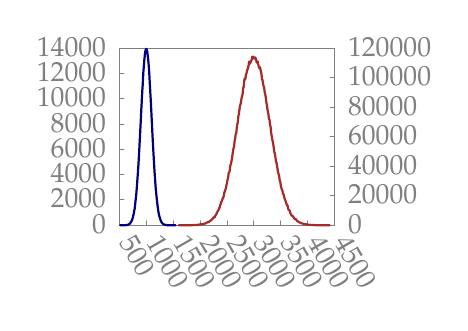
\begin{tikzpicture}[gnuplot, scale=0.3]
%% generated with GNUPLOT 5.2p2 (Lua 5.3; terminal rev. 99, script rev. 102)
%% wo 11 jul 2018 09:51:59 CEST
\path (0.000,0.000) rectangle (12.500,8.750);
\gpcolor{rgb color={0.502,0.502,0.502}}
\gpsetlinetype{gp lt border}
\gpsetdashtype{gp dt solid}
\gpsetlinewidth{1.00}
\draw[gp path] (1.380,0.945)--(1.560,0.945);
\node[gp node right] at (1.196,0.945) {$0$};
\draw[gp path] (1.380,2.016)--(1.560,2.016);
\node[gp node right] at (1.196,2.016) {$2000$};
\draw[gp path] (1.380,3.087)--(1.560,3.087);
\node[gp node right] at (1.196,3.087) {$4000$};
\draw[gp path] (1.380,4.158)--(1.560,4.158);
\node[gp node right] at (1.196,4.158) {$6000$};
\draw[gp path] (1.380,5.228)--(1.560,5.228);
\node[gp node right] at (1.196,5.228) {$8000$};
\draw[gp path] (1.380,6.299)--(1.560,6.299);
\node[gp node right] at (1.196,6.299) {$10000$};
\draw[gp path] (1.380,7.370)--(1.560,7.370);
\node[gp node right] at (1.196,7.370) {$12000$};
\draw[gp path] (1.380,8.441)--(1.560,8.441);
\node[gp node right] at (1.196,8.441) {$14000$};
\draw[gp path] (1.380,0.945)--(1.380,1.125);
\node[gp node left,rotate=-60] at (1.380,0.761) {$500$};
\draw[gp path] (2.517,0.945)--(2.517,1.125);
\node[gp node left,rotate=-60] at (2.517,0.761) {$1000$};
\draw[gp path] (3.654,0.945)--(3.654,1.125);
\node[gp node left,rotate=-60] at (3.654,0.761) {$1500$};
\draw[gp path] (4.791,0.945)--(4.791,1.125);
\node[gp node left,rotate=-60] at (4.791,0.761) {$2000$};
\draw[gp path] (5.928,0.945)--(5.928,1.125);
\node[gp node left,rotate=-60] at (5.928,0.761) {$2500$};
\draw[gp path] (7.064,0.945)--(7.064,1.125);
\node[gp node left,rotate=-60] at (7.064,0.761) {$3000$};
\draw[gp path] (8.201,0.945)--(8.201,1.125);
\node[gp node left,rotate=-60] at (8.201,0.761) {$3500$};
\draw[gp path] (9.338,0.945)--(9.338,1.125);
\node[gp node left,rotate=-60] at (9.338,0.761) {$4000$};
\draw[gp path] (10.475,0.945)--(10.475,1.125);
\node[gp node left,rotate=-60] at (10.475,0.761) {$4500$};
\draw[gp path] (10.475,0.945)--(10.295,0.945);
\node[gp node left] at (10.659,0.945) {$0$};
\draw[gp path] (10.475,2.194)--(10.295,2.194);
\node[gp node left] at (10.659,2.194) {$20000$};
\draw[gp path] (10.475,3.444)--(10.295,3.444);
\node[gp node left] at (10.659,3.444) {$40000$};
\draw[gp path] (10.475,4.693)--(10.295,4.693);
\node[gp node left] at (10.659,4.693) {$60000$};
\draw[gp path] (10.475,5.942)--(10.295,5.942);
\node[gp node left] at (10.659,5.942) {$80000$};
\draw[gp path] (10.475,7.192)--(10.295,7.192);
\node[gp node left] at (10.659,7.192) {$100000$};
\draw[gp path] (10.475,8.441)--(10.295,8.441);
\node[gp node left] at (10.659,8.441) {$120000$};
\draw[gp path] (1.380,8.441)--(1.380,0.945)--(10.475,0.945)--(10.475,8.441)--cycle;
\gpcolor{rgb color={0.647,0.165,0.165}}
\gpsetlinewidth{2.00}
\draw[gp path] (3.881,0.946)--(3.995,0.947)--(4.018,0.946)--(4.040,0.946)--(4.086,0.946)%
  --(4.109,0.946)--(4.131,0.946)--(4.154,0.947)--(4.177,0.946)--(4.199,0.947)--(4.245,0.946)%
  --(4.268,0.948)--(4.290,0.947)--(4.313,0.947)--(4.336,0.946)--(4.359,0.948)--(4.381,0.948)%
  --(4.404,0.948)--(4.427,0.948)--(4.450,0.951)--(4.472,0.947)--(4.495,0.951)--(4.518,0.952)%
  --(4.541,0.952)--(4.563,0.955)--(4.586,0.957)--(4.609,0.959)--(4.631,0.961)--(4.654,0.957)%
  --(4.677,0.962)--(4.700,0.964)--(4.722,0.964)--(4.745,0.973)--(4.768,0.973)--(4.791,0.981)%
  --(4.813,0.985)--(4.836,0.985)--(4.859,0.987)--(4.882,0.991)--(4.904,0.987)--(4.927,1.000)%
  --(4.950,1.004)--(4.973,1.013)--(4.995,1.015)--(5.018,1.024)--(5.041,1.034)--(5.063,1.054)%
  --(5.086,1.071)--(5.109,1.064)--(5.132,1.083)--(5.154,1.086)--(5.177,1.105)--(5.200,1.124)%
  --(5.223,1.136)--(5.245,1.148)--(5.268,1.173)--(5.291,1.192)--(5.314,1.220)--(5.336,1.243)%
  --(5.359,1.260)--(5.382,1.299)--(5.405,1.282)--(5.427,1.337)--(5.450,1.397)--(5.473,1.401)%
  --(5.495,1.469)--(5.518,1.520)--(5.541,1.559)--(5.564,1.583)--(5.586,1.674)--(5.609,1.675)%
  --(5.632,1.793)--(5.655,1.831)--(5.677,1.917)--(5.700,1.955)--(5.723,2.023)--(5.746,2.087)%
  --(5.768,2.122)--(5.791,2.203)--(5.814,2.337)--(5.837,2.389)--(5.859,2.453)--(5.882,2.523)%
  --(5.905,2.664)--(5.928,2.754)--(5.950,2.888)--(5.973,2.962)--(5.996,3.169)--(6.018,3.169)%
  --(6.041,3.267)--(6.064,3.467)--(6.087,3.531)--(6.109,3.629)--(6.132,3.752)--(6.155,3.914)%
  --(6.178,4.077)--(6.200,4.197)--(6.223,4.276)--(6.246,4.498)--(6.269,4.606)--(6.291,4.790)%
  --(6.314,4.828)--(6.337,5.049)--(6.360,5.222)--(6.382,5.302)--(6.405,5.548)--(6.428,5.661)%
  --(6.450,5.831)--(6.473,5.992)--(6.496,6.065)--(6.519,6.168)--(6.541,6.335)--(6.564,6.403)%
  --(6.587,6.510)--(6.610,6.752)--(6.632,6.806)--(6.655,7.076)--(6.678,7.165)--(6.701,7.122)%
  --(6.723,7.314)--(6.746,7.358)--(6.769,7.477)--(6.792,7.546)--(6.814,7.591)--(6.837,7.702)%
  --(6.860,7.871)--(6.882,7.865)--(6.905,7.787)--(6.928,7.866)--(6.951,7.914)--(6.973,7.970)%
  --(6.996,8.080)--(7.019,8.081)--(7.042,8.059)--(7.064,8.002)--(7.087,8.000)--(7.110,8.052)%
  --(7.133,8.016)--(7.155,7.974)--(7.178,7.837)--(7.201,7.874)--(7.224,7.878)--(7.246,7.751)%
  --(7.269,7.671)--(7.292,7.592)--(7.314,7.639)--(7.337,7.579)--(7.360,7.442)--(7.383,7.356)%
  --(7.405,7.134)--(7.428,7.087)--(7.451,6.935)--(7.474,6.828)--(7.496,6.778)--(7.519,6.591)%
  --(7.542,6.488)--(7.565,6.372)--(7.587,6.155)--(7.610,6.056)--(7.633,5.882)--(7.656,5.745)%
  --(7.678,5.649)--(7.701,5.435)--(7.724,5.422)--(7.747,5.204)--(7.769,5.117)--(7.792,4.876)%
  --(7.815,4.725)--(7.837,4.607)--(7.860,4.483)--(7.883,4.379)--(7.906,4.203)--(7.928,4.038)%
  --(7.951,3.972)--(7.974,3.829)--(7.997,3.648)--(8.019,3.594)--(8.042,3.465)--(8.065,3.309)%
  --(8.088,3.179)--(8.110,3.106)--(8.133,3.024)--(8.156,2.833)--(8.179,2.792)--(8.201,2.633)%
  --(8.224,2.533)--(8.247,2.452)--(8.269,2.422)--(8.292,2.295)--(8.315,2.251)--(8.338,2.187)%
  --(8.360,2.082)--(8.383,2.028)--(8.406,1.967)--(8.429,1.885)--(8.451,1.835)--(8.474,1.775)%
  --(8.497,1.765)--(8.520,1.622)--(8.542,1.583)--(8.565,1.581)--(8.588,1.537)--(8.611,1.449)%
  --(8.633,1.402)--(8.656,1.370)--(8.679,1.340)--(8.701,1.340)--(8.724,1.307)--(8.747,1.279)%
  --(8.770,1.219)--(8.792,1.217)--(8.815,1.208)--(8.838,1.204)--(8.861,1.173)--(8.883,1.132)%
  --(8.906,1.109)--(8.929,1.100)--(8.952,1.100)--(8.974,1.076)--(8.997,1.061)--(9.020,1.055)%
  --(9.043,1.053)--(9.065,1.032)--(9.088,1.024)--(9.111,1.022)--(9.133,1.018)--(9.156,1.005)%
  --(9.179,1.000)--(9.202,0.994)--(9.224,0.996)--(9.247,0.986)--(9.270,0.978)--(9.293,0.986)%
  --(9.315,0.975)--(9.338,0.969)--(9.361,0.966)--(9.384,0.968)--(9.406,0.962)--(9.429,0.965)%
  --(9.452,0.960)--(9.475,0.961)--(9.497,0.958)--(9.520,0.956)--(9.543,0.950)--(9.566,0.955)%
  --(9.588,0.953)--(9.611,0.952)--(9.634,0.950)--(9.656,0.948)--(9.679,0.948)--(9.702,0.947)%
  --(9.725,0.950)--(9.747,0.949)--(9.770,0.948)--(9.793,0.948)--(9.816,0.946)--(9.838,0.946)%
  --(9.861,0.947)--(9.884,0.946)--(9.929,0.947)--(9.952,0.946)--(9.975,0.947)--(9.998,0.946)%
  --(10.020,0.946)--(10.066,0.946)--(10.088,0.946)--(10.225,0.946)--(10.270,0.946);
\gpcolor{rgb color={0.000,0.000,0.502}}
\draw[gp path] (1.403,0.945)--(1.425,0.945)--(1.448,0.945)--(1.471,0.945)--(1.494,0.945)%
  --(1.516,0.946)--(1.539,0.946)--(1.562,0.946)--(1.585,0.947)--(1.607,0.949)--(1.630,0.949)%
  --(1.653,0.951)--(1.676,0.953)--(1.698,0.957)--(1.721,0.965)--(1.744,0.971)--(1.767,0.982)%
  --(1.789,0.999)--(1.812,1.013)--(1.835,1.042)--(1.857,1.077)--(1.880,1.112)--(1.903,1.162)%
  --(1.926,1.230)--(1.948,1.311)--(1.971,1.410)--(1.994,1.539)--(2.017,1.652)--(2.039,1.858)%
  --(2.062,2.058)--(2.085,2.280)--(2.108,2.549)--(2.130,2.868)--(2.153,3.180)--(2.176,3.524)%
  --(2.199,3.925)--(2.221,4.343)--(2.244,4.784)--(2.267,5.229)--(2.290,5.705)--(2.312,6.129)%
  --(2.335,6.572)--(2.358,6.935)--(2.380,7.381)--(2.403,7.676)--(2.426,7.953)--(2.449,8.197)%
  --(2.471,8.328)--(2.494,8.407)--(2.517,8.410)--(2.540,8.342)--(2.562,8.187)--(2.585,7.998)%
  --(2.608,7.738)--(2.631,7.424)--(2.653,7.001)--(2.676,6.606)--(2.699,6.188)--(2.722,5.740)%
  --(2.744,5.282)--(2.767,4.817)--(2.790,4.384)--(2.812,3.973)--(2.835,3.581)--(2.858,3.194)%
  --(2.881,2.881)--(2.903,2.551)--(2.926,2.309)--(2.949,2.083)--(2.972,1.877)--(2.994,1.702)%
  --(3.017,1.540)--(3.040,1.413)--(3.063,1.320)--(3.085,1.240)--(3.108,1.173)--(3.131,1.116)%
  --(3.154,1.075)--(3.176,1.042)--(3.199,1.016)--(3.222,0.995)--(3.244,0.984)--(3.267,0.972)%
  --(3.290,0.964)--(3.313,0.958)--(3.335,0.956)--(3.358,0.953)--(3.381,0.948)--(3.404,0.948)%
  --(3.426,0.947)--(3.449,0.947)--(3.472,0.946)--(3.495,0.946)--(3.517,0.945)--(3.540,0.945)%
  --(3.563,0.945)--(3.586,0.945)--(3.631,0.945)--(3.745,0.945);
%% coordinates of the plot area
\gpdefrectangularnode{gp plot 1}{\pgfpoint{1.380cm}{0.945cm}}{\pgfpoint{10.475cm}{8.441cm}}
\end{tikzpicture}
%% gnuplot variables

\end{tabular}
\end{center}
\caption{\label{fig:inputselection:normal_3to1_largest}
  Simulation of largest-first coin selection. Main histogram shows UTxO entries;
  inset graph shows UTxO balance in blue and UTxO size in red, histogram
  top-right shows number of inputs per transaction, graph bottom right shows the
  change:payment ratio (more on that below). Graph on the far right shows the
  distribution of deposits (blue, right axis) versus payments (red, left axis).
  In this case, both are normally distributed with a mean of 1000 and 3000
  respectively, and we have a deposit:payment ratio of 3:1; modelling a
  situation where we have frequent smaller deposits, and less frequent but
  larger payments (withdrawals). The wallet starts with an initial balance of
  1M.
}
\end{figure}

There are various things to see in this graph, but for now we want to focus
on the UTxO histogram and its size. Note that as time passes, the size of the
UTxO increases and increases, up to about 60k entries after about 1M
cycles (with 3 deposits and 1 payment per cycle). A wallet with 60k entries
is \emph{huge}, and looking at the UTxO histogram we can see why this happens:
virtually all of these entries are dust. We get more and more small outputs,
and those small outputs are getting smaller and smaller.

\subsection{Cleaning up}

Erhardt makes the following very astute observation:

\begin{quote}
``If 90\% of the UTxO is dust, then if we pick an unspent output
\emph{randomly}, we have a 90\% change of picking a dust output.''
\end{quote}

He concludes that this means that a coin selection algorithm that simply picks
unspent outputs \emph{at random} might be pretty effective; in particular,
effective at collecting dust. Indeed, it is. Consider the simulation shown in
Figure~\ref{fig:inputselection:normal_3to1_largeThenRandom}.

\begin{figure}[p]
\begin{center}
\scriptsize
\begin{tabular}{ll}
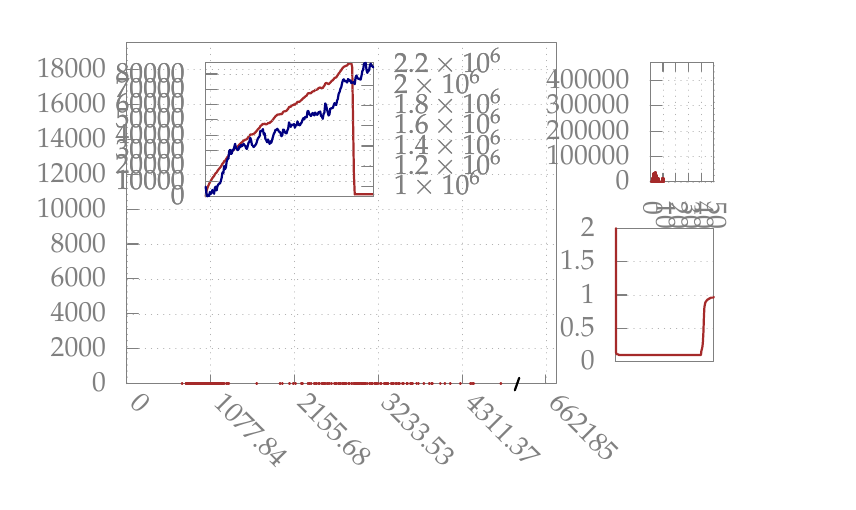
\begin{tikzpicture}[gnuplot, xscale=0.8, yscale=0.6]
%% generated with GNUPLOT 5.2p2 (Lua 5.3; terminal rev. 99, script rev. 102)
%% wo 11 jul 2018 10:15:19 CEST
\path (0.000,0.000) rectangle (12.500,8.750);
\gpcolor{color=gp lt color axes}
\gpsetlinetype{gp lt axes}
\gpsetdashtype{gp dt axes}
\gpsetlinewidth{0.50}
\draw[gp path] (1.380,1.218)--(8.197,1.218);
\gpcolor{rgb color={0.502,0.502,0.502}}
\gpsetlinetype{gp lt border}
\gpsetdashtype{gp dt solid}
\gpsetlinewidth{1.00}
\draw[gp path] (1.380,1.218)--(1.560,1.218);
\node[gp node right] at (1.196,1.218) {$0$};
\gpcolor{color=gp lt color axes}
\gpsetlinetype{gp lt axes}
\gpsetdashtype{gp dt axes}
\gpsetlinewidth{0.50}
\draw[gp path] (1.380,1.956)--(8.197,1.956);
\gpcolor{rgb color={0.502,0.502,0.502}}
\gpsetlinetype{gp lt border}
\gpsetdashtype{gp dt solid}
\gpsetlinewidth{1.00}
\draw[gp path] (1.380,1.956)--(1.560,1.956);
\node[gp node right] at (1.196,1.956) {$2000$};
\gpcolor{color=gp lt color axes}
\gpsetlinetype{gp lt axes}
\gpsetdashtype{gp dt axes}
\gpsetlinewidth{0.50}
\draw[gp path] (1.380,2.694)--(8.197,2.694);
\gpcolor{rgb color={0.502,0.502,0.502}}
\gpsetlinetype{gp lt border}
\gpsetdashtype{gp dt solid}
\gpsetlinewidth{1.00}
\draw[gp path] (1.380,2.694)--(1.560,2.694);
\node[gp node right] at (1.196,2.694) {$4000$};
\gpcolor{color=gp lt color axes}
\gpsetlinetype{gp lt axes}
\gpsetdashtype{gp dt axes}
\gpsetlinewidth{0.50}
\draw[gp path] (1.380,3.432)--(8.197,3.432);
\gpcolor{rgb color={0.502,0.502,0.502}}
\gpsetlinetype{gp lt border}
\gpsetdashtype{gp dt solid}
\gpsetlinewidth{1.00}
\draw[gp path] (1.380,3.432)--(1.560,3.432);
\node[gp node right] at (1.196,3.432) {$6000$};
\gpcolor{color=gp lt color axes}
\gpsetlinetype{gp lt axes}
\gpsetdashtype{gp dt axes}
\gpsetlinewidth{0.50}
\draw[gp path] (1.380,4.170)--(8.197,4.170);
\gpcolor{rgb color={0.502,0.502,0.502}}
\gpsetlinetype{gp lt border}
\gpsetdashtype{gp dt solid}
\gpsetlinewidth{1.00}
\draw[gp path] (1.380,4.170)--(1.560,4.170);
\node[gp node right] at (1.196,4.170) {$8000$};
\gpcolor{color=gp lt color axes}
\gpsetlinetype{gp lt axes}
\gpsetdashtype{gp dt axes}
\gpsetlinewidth{0.50}
\draw[gp path] (1.380,4.908)--(8.197,4.908);
\gpcolor{rgb color={0.502,0.502,0.502}}
\gpsetlinetype{gp lt border}
\gpsetdashtype{gp dt solid}
\gpsetlinewidth{1.00}
\draw[gp path] (1.380,4.908)--(1.560,4.908);
\node[gp node right] at (1.196,4.908) {$10000$};
\gpcolor{color=gp lt color axes}
\gpsetlinetype{gp lt axes}
\gpsetdashtype{gp dt axes}
\gpsetlinewidth{0.50}
\draw[gp path] (1.380,5.646)--(8.197,5.646);
\gpcolor{rgb color={0.502,0.502,0.502}}
\gpsetlinetype{gp lt border}
\gpsetdashtype{gp dt solid}
\gpsetlinewidth{1.00}
\draw[gp path] (1.380,5.646)--(1.560,5.646);
\node[gp node right] at (1.196,5.646) {$12000$};
\gpcolor{color=gp lt color axes}
\gpsetlinetype{gp lt axes}
\gpsetdashtype{gp dt axes}
\gpsetlinewidth{0.50}
\draw[gp path] (1.380,6.384)--(8.197,6.384);
\gpcolor{rgb color={0.502,0.502,0.502}}
\gpsetlinetype{gp lt border}
\gpsetdashtype{gp dt solid}
\gpsetlinewidth{1.00}
\draw[gp path] (1.380,6.384)--(1.560,6.384);
\node[gp node right] at (1.196,6.384) {$14000$};
\gpcolor{color=gp lt color axes}
\gpsetlinetype{gp lt axes}
\gpsetdashtype{gp dt axes}
\gpsetlinewidth{0.50}
\draw[gp path] (1.380,7.121)--(8.197,7.121);
\gpcolor{rgb color={0.502,0.502,0.502}}
\gpsetlinetype{gp lt border}
\gpsetdashtype{gp dt solid}
\gpsetlinewidth{1.00}
\draw[gp path] (1.380,7.121)--(1.560,7.121);
\node[gp node right] at (1.196,7.121) {$16000$};
\gpcolor{color=gp lt color axes}
\gpsetlinetype{gp lt axes}
\gpsetdashtype{gp dt axes}
\gpsetlinewidth{0.50}
\draw[gp path] (1.380,7.859)--(8.197,7.859);
\gpcolor{rgb color={0.502,0.502,0.502}}
\gpsetlinetype{gp lt border}
\gpsetdashtype{gp dt solid}
\gpsetlinewidth{1.00}
\draw[gp path] (1.380,7.859)--(1.560,7.859);
\node[gp node right] at (1.196,7.859) {$18000$};
\gpcolor{color=gp lt color axes}
\gpsetlinetype{gp lt axes}
\gpsetdashtype{gp dt axes}
\gpsetlinewidth{0.50}
\draw[gp path] (1.380,1.218)--(1.380,8.441);
\gpcolor{rgb color={0.502,0.502,0.502}}
\gpsetlinetype{gp lt border}
\gpsetdashtype{gp dt solid}
\gpsetlinewidth{1.00}
\draw[gp path] (1.380,1.218)--(1.380,1.398);
\node[gp node left,rotate=-45] at (1.380,1.034) {$0$};
\gpcolor{color=gp lt color axes}
\gpsetlinetype{gp lt axes}
\gpsetdashtype{gp dt axes}
\gpsetlinewidth{0.50}
\draw[gp path] (2.710,1.218)--(2.710,8.441);
\gpcolor{rgb color={0.502,0.502,0.502}}
\gpsetlinetype{gp lt border}
\gpsetdashtype{gp dt solid}
\gpsetlinewidth{1.00}
\draw[gp path] (2.710,1.218)--(2.710,1.398);
\node[gp node left,rotate=-45] at (2.710,1.034) {$1077.84$};
\gpcolor{color=gp lt color axes}
\gpsetlinetype{gp lt axes}
\gpsetdashtype{gp dt axes}
\gpsetlinewidth{0.50}
\draw[gp path] (4.040,1.218)--(4.040,8.441);
\gpcolor{rgb color={0.502,0.502,0.502}}
\gpsetlinetype{gp lt border}
\gpsetdashtype{gp dt solid}
\gpsetlinewidth{1.00}
\draw[gp path] (4.040,1.218)--(4.040,1.398);
\node[gp node left,rotate=-45] at (4.040,1.034) {$2155.68$};
\gpcolor{color=gp lt color axes}
\gpsetlinetype{gp lt axes}
\gpsetdashtype{gp dt axes}
\gpsetlinewidth{0.50}
\draw[gp path] (5.370,1.218)--(5.370,8.441);
\gpcolor{rgb color={0.502,0.502,0.502}}
\gpsetlinetype{gp lt border}
\gpsetdashtype{gp dt solid}
\gpsetlinewidth{1.00}
\draw[gp path] (5.370,1.218)--(5.370,1.398);
\node[gp node left,rotate=-45] at (5.370,1.034) {$3233.53$};
\gpcolor{color=gp lt color axes}
\gpsetlinetype{gp lt axes}
\gpsetdashtype{gp dt axes}
\gpsetlinewidth{0.50}
\draw[gp path] (6.701,1.218)--(6.701,8.441);
\gpcolor{rgb color={0.502,0.502,0.502}}
\gpsetlinetype{gp lt border}
\gpsetdashtype{gp dt solid}
\gpsetlinewidth{1.00}
\draw[gp path] (6.701,1.218)--(6.701,1.398);
\node[gp node left,rotate=-45] at (6.701,1.034) {$4311.37$};
\gpcolor{color=gp lt color axes}
\gpsetlinetype{gp lt axes}
\gpsetdashtype{gp dt axes}
\gpsetlinewidth{0.50}
\draw[gp path] (8.031,1.218)--(8.031,8.441);
\gpcolor{rgb color={0.502,0.502,0.502}}
\gpsetlinetype{gp lt border}
\gpsetdashtype{gp dt solid}
\gpsetlinewidth{1.00}
\draw[gp path] (8.031,1.218)--(8.031,1.398);
\node[gp node left,rotate=-45] at (8.031,1.034) {$662185$};
\draw[gp path] (1.380,8.441)--(1.380,1.218)--(8.197,1.218)--(8.197,8.441)--cycle;
\gpcolor{rgb color={0.647,0.165,0.165}}
\gpsetlinewidth{2.00}
\draw[gp path] (2.250,1.218)--(2.262,1.218)--cycle;
\draw[gp path] (2.312,1.218)--(2.324,1.218)--cycle;
\draw[gp path] (2.324,1.218)--(2.324,1.219)--(2.336,1.219)--(2.336,1.218)--cycle;
\draw[gp path] (2.336,1.218)--(2.349,1.218)--cycle;
\draw[gp path] (2.349,1.218)--(2.349,1.219)--(2.361,1.219)--(2.361,1.218)--cycle;
\draw[gp path] (2.361,1.218)--(2.361,1.221)--(2.373,1.221)--(2.373,1.218)--cycle;
\draw[gp path] (2.373,1.218)--(2.373,1.220)--(2.386,1.220)--(2.386,1.218)--cycle;
\draw[gp path] (2.386,1.218)--(2.386,1.220)--(2.398,1.220)--(2.398,1.218)--cycle;
\draw[gp path] (2.398,1.218)--(2.398,1.222)--(2.410,1.222)--(2.410,1.218)--cycle;
\draw[gp path] (2.410,1.218)--(2.410,1.222)--(2.423,1.222)--(2.423,1.218)--cycle;
\draw[gp path] (2.423,1.218)--(2.423,1.222)--(2.435,1.222)--(2.435,1.218)--cycle;
\draw[gp path] (2.435,1.218)--(2.435,1.223)--(2.447,1.223)--(2.447,1.218)--cycle;
\draw[gp path] (2.447,1.218)--(2.447,1.222)--(2.460,1.222)--(2.460,1.218)--cycle;
\draw[gp path] (2.460,1.218)--(2.460,1.225)--(2.472,1.225)--(2.472,1.218)--cycle;
\draw[gp path] (2.472,1.218)--(2.472,1.225)--(2.485,1.225)--(2.485,1.218)--cycle;
\draw[gp path] (2.485,1.218)--(2.485,1.226)--(2.497,1.226)--(2.497,1.218)--cycle;
\draw[gp path] (2.497,1.218)--(2.497,1.226)--(2.509,1.226)--(2.509,1.218)--cycle;
\draw[gp path] (2.509,1.218)--(2.509,1.229)--(2.522,1.229)--(2.522,1.218)--cycle;
\draw[gp path] (2.522,1.218)--(2.522,1.227)--(2.534,1.227)--(2.534,1.218)--cycle;
\draw[gp path] (2.534,1.218)--(2.534,1.230)--(2.546,1.230)--(2.546,1.218)--cycle;
\draw[gp path] (2.546,1.218)--(2.546,1.229)--(2.559,1.229)--(2.559,1.218)--cycle;
\draw[gp path] (2.559,1.218)--(2.559,1.233)--(2.571,1.233)--(2.571,1.218)--cycle;
\draw[gp path] (2.571,1.218)--(2.571,1.231)--(2.583,1.231)--(2.583,1.218)--cycle;
\draw[gp path] (2.583,1.218)--(2.583,1.233)--(2.596,1.233)--(2.596,1.218)--cycle;
\draw[gp path] (2.596,1.218)--(2.596,1.233)--(2.608,1.233)--(2.608,1.218)--cycle;
\draw[gp path] (2.608,1.218)--(2.608,1.233)--(2.620,1.233)--(2.620,1.218)--cycle;
\draw[gp path] (2.620,1.218)--(2.620,1.235)--(2.633,1.235)--(2.633,1.218)--cycle;
\draw[gp path] (2.633,1.218)--(2.633,1.228)--(2.645,1.228)--(2.645,1.218)--cycle;
\draw[gp path] (2.645,1.218)--(2.645,1.228)--(2.657,1.228)--(2.657,1.218)--cycle;
\draw[gp path] (2.657,1.218)--(2.657,1.232)--(2.670,1.232)--(2.670,1.218)--cycle;
\draw[gp path] (2.670,1.218)--(2.670,1.229)--(2.682,1.229)--(2.682,1.218)--cycle;
\draw[gp path] (2.682,1.218)--(2.682,1.231)--(2.694,1.231)--(2.694,1.218)--cycle;
\draw[gp path] (2.694,1.218)--(2.694,1.231)--(2.707,1.231)--(2.707,1.218)--cycle;
\draw[gp path] (2.707,1.218)--(2.707,1.228)--(2.719,1.228)--(2.719,1.218)--cycle;
\draw[gp path] (2.719,1.218)--(2.719,1.222)--(2.731,1.222)--(2.731,1.218)--cycle;
\draw[gp path] (2.731,1.218)--(2.731,1.225)--(2.744,1.225)--(2.744,1.218)--cycle;
\draw[gp path] (2.744,1.218)--(2.744,1.224)--(2.756,1.224)--(2.756,1.218)--cycle;
\draw[gp path] (2.756,1.218)--(2.756,1.225)--(2.768,1.225)--(2.768,1.218)--cycle;
\draw[gp path] (2.768,1.218)--(2.768,1.224)--(2.781,1.224)--(2.781,1.218)--cycle;
\draw[gp path] (2.781,1.218)--(2.781,1.223)--(2.793,1.223)--(2.793,1.218)--cycle;
\draw[gp path] (2.793,1.218)--(2.793,1.221)--(2.805,1.221)--(2.805,1.218)--cycle;
\draw[gp path] (2.805,1.218)--(2.805,1.222)--(2.818,1.222)--(2.818,1.218)--cycle;
\draw[gp path] (2.818,1.218)--(2.818,1.222)--(2.830,1.222)--(2.830,1.218)--cycle;
\draw[gp path] (2.830,1.218)--(2.830,1.220)--(2.842,1.220)--(2.842,1.218)--cycle;
\draw[gp path] (2.842,1.218)--(2.842,1.219)--(2.855,1.219)--(2.855,1.218)--cycle;
\draw[gp path] (2.855,1.218)--(2.855,1.220)--(2.867,1.220)--(2.867,1.218)--cycle;
\draw[gp path] (2.867,1.218)--(2.867,1.219)--(2.879,1.219)--(2.879,1.218)--cycle;
\draw[gp path] (2.879,1.218)--(2.892,1.218)--cycle;
\draw[gp path] (2.892,1.218)--(2.892,1.219)--(2.904,1.219)--(2.904,1.218)--cycle;
\draw[gp path] (2.904,1.218)--(2.916,1.218)--cycle;
\draw[gp path] (2.916,1.218)--(2.929,1.218)--cycle;
\draw[gp path] (2.953,1.218)--(2.966,1.218)--cycle;
\draw[gp path] (2.978,1.218)--(2.978,1.219)--(2.990,1.219)--(2.990,1.218)--cycle;
\draw[gp path] (2.990,1.218)--(3.003,1.218)--cycle;
\draw[gp path] (3.435,1.218)--(3.447,1.218)--cycle;
\draw[gp path] (3.805,1.218)--(3.817,1.218)--cycle;
\draw[gp path] (3.842,1.218)--(3.854,1.218)--cycle;
\draw[gp path] (3.953,1.218)--(3.953,1.219)--(3.965,1.219)--(3.965,1.218)--cycle;
\draw[gp path] (4.015,1.218)--(4.027,1.218)--cycle;
\draw[gp path] (4.052,1.218)--(4.052,1.219)--(4.064,1.219)--(4.064,1.218)--cycle;
\draw[gp path] (4.138,1.218)--(4.138,1.219)--(4.151,1.219)--(4.151,1.218)--cycle;
\draw[gp path] (4.151,1.218)--(4.151,1.219)--(4.163,1.219)--(4.163,1.218)--cycle;
\draw[gp path] (4.163,1.218)--(4.163,1.219)--(4.175,1.219)--(4.175,1.218)--cycle;
\draw[gp path] (4.249,1.218)--(4.262,1.218)--cycle;
\draw[gp path] (4.274,1.218)--(4.286,1.218)--cycle;
\draw[gp path] (4.299,1.218)--(4.311,1.218)--cycle;
\draw[gp path] (4.348,1.218)--(4.360,1.218)--cycle;
\draw[gp path] (4.373,1.218)--(4.385,1.218)--cycle;
\draw[gp path] (4.385,1.218)--(4.385,1.219)--(4.397,1.219)--(4.397,1.218)--cycle;
\draw[gp path] (4.410,1.218)--(4.410,1.219)--(4.422,1.219)--(4.422,1.218)--cycle;
\draw[gp path] (4.434,1.218)--(4.434,1.219)--(4.447,1.219)--(4.447,1.218)--cycle;
\draw[gp path] (4.471,1.218)--(4.484,1.218)--cycle;
\draw[gp path] (4.484,1.218)--(4.496,1.218)--cycle;
\draw[gp path] (4.496,1.218)--(4.496,1.219)--(4.508,1.219)--(4.508,1.218)--cycle;
\draw[gp path] (4.508,1.218)--(4.508,1.219)--(4.521,1.219)--(4.521,1.218)--cycle;
\draw[gp path] (4.533,1.218)--(4.545,1.218)--cycle;
\draw[gp path] (4.558,1.218)--(4.570,1.218)--cycle;
\draw[gp path] (4.570,1.218)--(4.570,1.219)--(4.582,1.219)--(4.582,1.218)--cycle;
\draw[gp path] (4.595,1.218)--(4.595,1.219)--(4.607,1.219)--(4.607,1.218)--cycle;
\draw[gp path] (4.619,1.218)--(4.619,1.219)--(4.632,1.219)--(4.632,1.218)--cycle;
\draw[gp path] (4.669,1.218)--(4.669,1.220)--(4.681,1.220)--(4.681,1.218)--cycle;
\draw[gp path] (4.681,1.218)--(4.694,1.218)--cycle;
\draw[gp path] (4.694,1.218)--(4.694,1.219)--(4.706,1.219)--(4.706,1.218)--cycle;
\draw[gp path] (4.706,1.218)--(4.706,1.219)--(4.718,1.219)--(4.718,1.218)--cycle;
\draw[gp path] (4.731,1.218)--(4.743,1.218)--cycle;
\draw[gp path] (4.743,1.218)--(4.755,1.218)--cycle;
\draw[gp path] (4.755,1.218)--(4.768,1.218)--cycle;
\draw[gp path] (4.768,1.218)--(4.780,1.218)--cycle;
\draw[gp path] (4.792,1.218)--(4.792,1.219)--(4.805,1.219)--(4.805,1.218)--cycle;
\draw[gp path] (4.805,1.218)--(4.817,1.218)--cycle;
\draw[gp path] (4.817,1.218)--(4.817,1.219)--(4.829,1.219)--(4.829,1.218)--cycle;
\draw[gp path] (4.829,1.218)--(4.842,1.218)--cycle;
\draw[gp path] (4.842,1.218)--(4.842,1.219)--(4.854,1.219)--(4.854,1.218)--cycle;
\draw[gp path] (4.854,1.218)--(4.854,1.219)--(4.866,1.219)--(4.866,1.218)--cycle;
\draw[gp path] (4.891,1.218)--(4.891,1.219)--(4.903,1.219)--(4.903,1.218)--cycle;
\draw[gp path] (4.903,1.218)--(4.916,1.218)--cycle;
\draw[gp path] (4.940,1.218)--(4.940,1.219)--(4.953,1.219)--(4.953,1.218)--cycle;
\draw[gp path] (4.965,1.218)--(4.977,1.218)--cycle;
\draw[gp path] (4.990,1.218)--(4.990,1.219)--(5.002,1.219)--(5.002,1.218)--cycle;
\draw[gp path] (5.002,1.218)--(5.002,1.219)--(5.014,1.219)--(5.014,1.218)--cycle;
\draw[gp path] (5.014,1.218)--(5.027,1.218)--cycle;
\draw[gp path] (5.027,1.218)--(5.027,1.220)--(5.039,1.220)--(5.039,1.218)--cycle;
\draw[gp path] (5.039,1.218)--(5.039,1.219)--(5.051,1.219)--(5.051,1.218)--cycle;
\draw[gp path] (5.051,1.218)--(5.064,1.218)--cycle;
\draw[gp path] (5.064,1.218)--(5.076,1.218)--cycle;
\draw[gp path] (5.088,1.218)--(5.088,1.220)--(5.101,1.220)--(5.101,1.218)--cycle;
\draw[gp path] (5.101,1.218)--(5.101,1.219)--(5.113,1.219)--(5.113,1.218)--cycle;
\draw[gp path] (5.113,1.218)--(5.113,1.219)--(5.125,1.219)--(5.125,1.218)--cycle;
\draw[gp path] (5.125,1.218)--(5.125,1.219)--(5.138,1.219)--(5.138,1.218)--cycle;
\draw[gp path] (5.138,1.218)--(5.138,1.219)--(5.150,1.219)--(5.150,1.218)--cycle;
\draw[gp path] (5.150,1.218)--(5.162,1.218)--cycle;
\draw[gp path] (5.162,1.218)--(5.175,1.218)--cycle;
\draw[gp path] (5.187,1.218)--(5.199,1.218)--cycle;
\draw[gp path] (5.224,1.218)--(5.224,1.219)--(5.237,1.219)--(5.237,1.218)--cycle;
\draw[gp path] (5.249,1.218)--(5.261,1.218)--cycle;
\draw[gp path] (5.261,1.218)--(5.261,1.219)--(5.274,1.219)--(5.274,1.218)--cycle;
\draw[gp path] (5.274,1.218)--(5.274,1.219)--(5.286,1.219)--(5.286,1.218)--cycle;
\draw[gp path] (5.311,1.218)--(5.311,1.219)--(5.323,1.219)--(5.323,1.218)--cycle;
\draw[gp path] (5.323,1.218)--(5.323,1.219)--(5.335,1.219)--(5.335,1.218)--cycle;
\draw[gp path] (5.335,1.218)--(5.348,1.218)--cycle;
\draw[gp path] (5.360,1.218)--(5.372,1.218)--cycle;
\draw[gp path] (5.397,1.218)--(5.409,1.218)--cycle;
\draw[gp path] (5.409,1.218)--(5.409,1.219)--(5.422,1.219)--(5.422,1.218)--cycle;
\draw[gp path] (5.459,1.218)--(5.471,1.218)--cycle;
\draw[gp path] (5.471,1.218)--(5.483,1.218)--cycle;
\draw[gp path] (5.483,1.218)--(5.496,1.218)--cycle;
\draw[gp path] (5.496,1.218)--(5.508,1.218)--cycle;
\draw[gp path] (5.508,1.218)--(5.520,1.218)--cycle;
\draw[gp path] (5.520,1.218)--(5.533,1.218)--cycle;
\draw[gp path] (5.570,1.218)--(5.582,1.218)--cycle;
\draw[gp path] (5.594,1.218)--(5.594,1.219)--(5.607,1.219)--(5.607,1.218)--cycle;
\draw[gp path] (5.607,1.218)--(5.619,1.218)--cycle;
\draw[gp path] (5.631,1.218)--(5.631,1.219)--(5.644,1.219)--(5.644,1.218)--cycle;
\draw[gp path] (5.656,1.218)--(5.668,1.218)--cycle;
\draw[gp path] (5.681,1.218)--(5.693,1.218)--cycle;
\draw[gp path] (5.705,1.218)--(5.705,1.219)--(5.718,1.219)--(5.718,1.218)--cycle;
\draw[gp path] (5.742,1.218)--(5.742,1.219)--(5.755,1.219)--(5.755,1.218)--cycle;
\draw[gp path] (5.755,1.218)--(5.767,1.218)--cycle;
\draw[gp path] (5.767,1.218)--(5.767,1.219)--(5.780,1.219)--(5.780,1.218)--cycle;
\draw[gp path] (5.817,1.218)--(5.829,1.218)--cycle;
\draw[gp path] (5.829,1.218)--(5.829,1.219)--(5.841,1.219)--(5.841,1.218)--cycle;
\draw[gp path] (5.878,1.218)--(5.878,1.219)--(5.891,1.219)--(5.891,1.218)--cycle;
\draw[gp path] (5.891,1.218)--(5.903,1.218)--cycle;
\draw[gp path] (5.903,1.218)--(5.915,1.218)--cycle;
\draw[gp path] (5.915,1.218)--(5.915,1.219)--(5.928,1.219)--(5.928,1.218)--cycle;
\draw[gp path] (5.977,1.218)--(5.977,1.219)--(5.989,1.219)--(5.989,1.218)--cycle;
\draw[gp path] (6.002,1.218)--(6.014,1.218)--cycle;
\draw[gp path] (6.088,1.218)--(6.100,1.218)--cycle;
\draw[gp path] (6.174,1.218)--(6.187,1.218)--cycle;
\draw[gp path] (6.211,1.218)--(6.224,1.218)--cycle;
\draw[gp path] (6.224,1.218)--(6.236,1.218)--cycle;
\draw[gp path] (6.347,1.218)--(6.347,1.219)--(6.360,1.219)--(6.360,1.218)--cycle;
\draw[gp path] (6.421,1.218)--(6.434,1.218)--cycle;
\draw[gp path] (6.508,1.218)--(6.520,1.218)--cycle;
\draw[gp path] (6.668,1.218)--(6.680,1.218)--cycle;
\draw[gp path] (6.828,1.218)--(6.841,1.218)--cycle;
\draw[gp path] (6.853,1.218)--(6.865,1.218)--cycle;
\draw[gp path] (6.878,1.218)--(6.890,1.218)--cycle;
\draw[gp path] (7.310,1.218)--(7.322,1.218)--cycle;
\gpcolor{color=gp lt color border}
\draw[gp path](7.538,1.074)--(7.608,1.337);
%% coordinates of the plot area
\gpdefrectangularnode{gp plot 1}{\pgfpoint{1.380cm}{1.218cm}}{\pgfpoint{8.197cm}{8.441cm}}
\gpcolor{color=gp lt color axes}
\gpsetlinetype{gp lt axes}
\gpsetdashtype{gp dt axes}
\gpsetlinewidth{0.50}
\draw[gp path] (2.630,5.180)--(5.291,5.180);
\gpcolor{rgb color={0.502,0.502,0.502}}
\gpsetlinetype{gp lt border}
\gpsetdashtype{gp dt solid}
\gpsetlinewidth{1.00}
\draw[gp path] (2.630,5.180)--(2.810,5.180);
\node[gp node right] at (2.446,5.180) {$0$};
\gpcolor{color=gp lt color axes}
\gpsetlinetype{gp lt axes}
\gpsetdashtype{gp dt axes}
\gpsetlinewidth{0.50}
\draw[gp path] (2.630,5.503)--(5.291,5.503);
\gpcolor{rgb color={0.502,0.502,0.502}}
\gpsetlinetype{gp lt border}
\gpsetdashtype{gp dt solid}
\gpsetlinewidth{1.00}
\draw[gp path] (2.630,5.503)--(2.810,5.503);
\node[gp node right] at (2.446,5.503) {$10000$};
\gpcolor{color=gp lt color axes}
\gpsetlinetype{gp lt axes}
\gpsetdashtype{gp dt axes}
\gpsetlinewidth{0.50}
\draw[gp path] (2.630,5.827)--(5.291,5.827);
\gpcolor{rgb color={0.502,0.502,0.502}}
\gpsetlinetype{gp lt border}
\gpsetdashtype{gp dt solid}
\gpsetlinewidth{1.00}
\draw[gp path] (2.630,5.827)--(2.810,5.827);
\node[gp node right] at (2.446,5.827) {$20000$};
\gpcolor{color=gp lt color axes}
\gpsetlinetype{gp lt axes}
\gpsetdashtype{gp dt axes}
\gpsetlinewidth{0.50}
\draw[gp path] (2.630,6.151)--(5.291,6.151);
\gpcolor{rgb color={0.502,0.502,0.502}}
\gpsetlinetype{gp lt border}
\gpsetdashtype{gp dt solid}
\gpsetlinewidth{1.00}
\draw[gp path] (2.630,6.151)--(2.810,6.151);
\node[gp node right] at (2.446,6.151) {$30000$};
\gpcolor{color=gp lt color axes}
\gpsetlinetype{gp lt axes}
\gpsetdashtype{gp dt axes}
\gpsetlinewidth{0.50}
\draw[gp path] (2.630,6.474)--(5.291,6.474);
\gpcolor{rgb color={0.502,0.502,0.502}}
\gpsetlinetype{gp lt border}
\gpsetdashtype{gp dt solid}
\gpsetlinewidth{1.00}
\draw[gp path] (2.630,6.474)--(2.810,6.474);
\node[gp node right] at (2.446,6.474) {$40000$};
\gpcolor{color=gp lt color axes}
\gpsetlinetype{gp lt axes}
\gpsetdashtype{gp dt axes}
\gpsetlinewidth{0.50}
\draw[gp path] (2.630,6.798)--(5.291,6.798);
\gpcolor{rgb color={0.502,0.502,0.502}}
\gpsetlinetype{gp lt border}
\gpsetdashtype{gp dt solid}
\gpsetlinewidth{1.00}
\draw[gp path] (2.630,6.798)--(2.810,6.798);
\node[gp node right] at (2.446,6.798) {$50000$};
\gpcolor{color=gp lt color axes}
\gpsetlinetype{gp lt axes}
\gpsetdashtype{gp dt axes}
\gpsetlinewidth{0.50}
\draw[gp path] (2.630,7.121)--(5.291,7.121);
\gpcolor{rgb color={0.502,0.502,0.502}}
\gpsetlinetype{gp lt border}
\gpsetdashtype{gp dt solid}
\gpsetlinewidth{1.00}
\draw[gp path] (2.630,7.121)--(2.810,7.121);
\node[gp node right] at (2.446,7.121) {$60000$};
\gpcolor{color=gp lt color axes}
\gpsetlinetype{gp lt axes}
\gpsetdashtype{gp dt axes}
\gpsetlinewidth{0.50}
\draw[gp path] (2.630,7.445)--(5.291,7.445);
\gpcolor{rgb color={0.502,0.502,0.502}}
\gpsetlinetype{gp lt border}
\gpsetdashtype{gp dt solid}
\gpsetlinewidth{1.00}
\draw[gp path] (2.630,7.445)--(2.810,7.445);
\node[gp node right] at (2.446,7.445) {$70000$};
\gpcolor{color=gp lt color axes}
\gpsetlinetype{gp lt axes}
\gpsetdashtype{gp dt axes}
\gpsetlinewidth{0.50}
\draw[gp path] (2.630,7.769)--(5.291,7.769);
\gpcolor{rgb color={0.502,0.502,0.502}}
\gpsetlinetype{gp lt border}
\gpsetdashtype{gp dt solid}
\gpsetlinewidth{1.00}
\draw[gp path] (2.630,7.769)--(2.810,7.769);
\node[gp node right] at (2.446,7.769) {$80000$};
\draw[gp path] (5.291,5.385)--(5.111,5.385);
\node[gp node left] at (5.475,5.385) {$1\times10^{6}$};
\draw[gp path] (5.291,5.815)--(5.111,5.815);
\node[gp node left] at (5.475,5.815) {$1.2\times10^{6}$};
\draw[gp path] (5.291,6.245)--(5.111,6.245);
\node[gp node left] at (5.475,6.245) {$1.4\times10^{6}$};
\draw[gp path] (5.291,6.675)--(5.111,6.675);
\node[gp node left] at (5.475,6.675) {$1.6\times10^{6}$};
\draw[gp path] (5.291,7.104)--(5.111,7.104);
\node[gp node left] at (5.475,7.104) {$1.8\times10^{6}$};
\draw[gp path] (5.291,7.534)--(5.111,7.534);
\node[gp node left] at (5.475,7.534) {$2\times10^{6}$};
\draw[gp path] (5.291,7.964)--(5.111,7.964);
\node[gp node left] at (5.475,7.964) {$2.2\times10^{6}$};
\draw[gp path] (2.630,8.004)--(2.630,5.180)--(5.291,5.180)--(5.291,8.004)--cycle;
\gpcolor{rgb color={0.647,0.165,0.165}}
\gpsetlinewidth{2.00}
\draw[gp path] (2.630,5.180)--(2.643,5.293)--(2.657,5.350)--(2.670,5.398)--(2.683,5.436)%
  --(2.697,5.476)--(2.710,5.504)--(2.724,5.536)--(2.737,5.567)--(2.750,5.588)--(2.764,5.610)%
  --(2.777,5.645)--(2.790,5.671)--(2.804,5.684)--(2.817,5.716)--(2.831,5.741)--(2.844,5.764)%
  --(2.857,5.784)--(2.871,5.808)--(2.884,5.836)--(2.897,5.869)--(2.911,5.886)--(2.924,5.923)%
  --(2.938,5.933)--(2.951,5.955)--(2.964,5.988)--(2.978,6.015)--(2.991,6.032)--(3.004,6.072)%
  --(3.018,6.095)--(3.031,6.099)--(3.045,6.115)--(3.058,6.145)--(3.071,6.159)--(3.085,6.185)%
  --(3.098,6.211)--(3.111,6.211)--(3.125,6.223)--(3.138,6.235)--(3.152,6.253)--(3.165,6.278)%
  --(3.178,6.289)--(3.192,6.310)--(3.205,6.321)--(3.218,6.338)--(3.232,6.359)--(3.245,6.367)%
  --(3.258,6.378)--(3.272,6.382)--(3.285,6.392)--(3.299,6.417)--(3.312,6.443)--(3.325,6.460)%
  --(3.339,6.487)--(3.352,6.490)--(3.365,6.487)--(3.379,6.495)--(3.392,6.500)--(3.406,6.516)%
  --(3.419,6.532)--(3.432,6.552)--(3.446,6.576)--(3.459,6.599)--(3.472,6.615)--(3.486,6.633)%
  --(3.499,6.666)--(3.513,6.681)--(3.526,6.696)--(3.539,6.716)--(3.553,6.704)--(3.566,6.720)%
  --(3.579,6.706)--(3.593,6.706)--(3.606,6.709)--(3.620,6.730)--(3.633,6.732)--(3.646,6.731)%
  --(3.660,6.756)--(3.673,6.762)--(3.686,6.782)--(3.700,6.804)--(3.713,6.832)--(3.726,6.851)%
  --(3.740,6.876)--(3.753,6.888)--(3.767,6.907)--(3.780,6.912)--(3.793,6.911)--(3.807,6.916)%
  --(3.820,6.924)--(3.833,6.917)--(3.847,6.931)--(3.860,6.966)--(3.874,6.979)--(3.887,6.978)%
  --(3.900,6.983)--(3.914,6.992)--(3.927,7.014)--(3.940,7.033)--(3.954,7.068)--(3.967,7.077)%
  --(3.981,7.075)--(3.994,7.099)--(4.007,7.106)--(4.021,7.113)--(4.034,7.127)--(4.047,7.117)%
  --(4.061,7.140)--(4.074,7.151)--(4.088,7.179)--(4.101,7.182)--(4.114,7.179)--(4.128,7.190)%
  --(4.141,7.207)--(4.154,7.223)--(4.168,7.241)--(4.181,7.262)--(4.195,7.270)--(4.208,7.290)%
  --(4.221,7.302)--(4.235,7.314)--(4.248,7.349)--(4.261,7.363)--(4.275,7.361)--(4.288,7.366)%
  --(4.301,7.360)--(4.315,7.384)--(4.328,7.399)--(4.342,7.403)--(4.355,7.408)--(4.368,7.432)%
  --(4.382,7.436)--(4.395,7.438)--(4.408,7.447)--(4.422,7.469)--(4.435,7.479)--(4.449,7.485)%
  --(4.462,7.470)--(4.475,7.475)--(4.489,7.472)--(4.502,7.501)--(4.515,7.522)--(4.529,7.565)%
  --(4.542,7.580)--(4.556,7.574)--(4.569,7.566)--(4.582,7.554)--(4.596,7.570)--(4.609,7.587)%
  --(4.622,7.610)--(4.636,7.629)--(4.649,7.636)--(4.663,7.662)--(4.676,7.685)--(4.689,7.693)%
  --(4.703,7.696)--(4.716,7.725)--(4.729,7.749)--(4.743,7.782)--(4.756,7.800)--(4.769,7.829)%
  --(4.783,7.850)--(4.796,7.879)--(4.810,7.904)--(4.823,7.922)--(4.836,7.929)--(4.850,7.937)%
  --(4.863,7.946)--(4.876,7.950)--(4.890,7.977)--(4.903,7.987)--(4.917,7.990)--(4.930,8.004)%
  --(4.943,7.996)--(4.957,7.912)--(4.970,6.796)--(4.983,5.680)--(4.997,5.221)--(5.010,5.222)%
  --(5.024,5.223)--(5.037,5.222)--(5.050,5.222)--(5.064,5.222)--(5.077,5.222)--(5.090,5.222)%
  --(5.104,5.223)--(5.117,5.223)--(5.131,5.224)--(5.144,5.225)--(5.157,5.224)--(5.171,5.225)%
  --(5.184,5.223)--(5.197,5.224)--(5.211,5.223)--(5.224,5.224)--(5.238,5.225)--(5.251,5.226)%
  --(5.264,5.225)--(5.278,5.226)--(5.291,5.223);
%% coordinates of the plot area
\gpdefrectangularnode{gp plot 2}{\pgfpoint{2.630cm}{5.180cm}}{\pgfpoint{5.291cm}{8.004cm}}
\gpcolor{color=gp lt color axes}
\gpsetlinetype{gp lt axes}
\gpsetdashtype{gp dt axes}
\gpsetlinewidth{0.50}
\draw[gp path] (2.630,5.180)--(5.291,5.180);
\gpcolor{rgb color={0.502,0.502,0.502}}
\gpsetlinetype{gp lt border}
\gpsetdashtype{gp dt solid}
\gpsetlinewidth{1.00}
\draw[gp path] (2.630,5.180)--(2.810,5.180);
\node[gp node right] at (2.446,5.180) {$0$};
\gpcolor{color=gp lt color axes}
\gpsetlinetype{gp lt axes}
\gpsetdashtype{gp dt axes}
\gpsetlinewidth{0.50}
\draw[gp path] (2.630,5.503)--(5.291,5.503);
\gpcolor{rgb color={0.502,0.502,0.502}}
\gpsetlinetype{gp lt border}
\gpsetdashtype{gp dt solid}
\gpsetlinewidth{1.00}
\draw[gp path] (2.630,5.503)--(2.810,5.503);
\node[gp node right] at (2.446,5.503) {$10000$};
\gpcolor{color=gp lt color axes}
\gpsetlinetype{gp lt axes}
\gpsetdashtype{gp dt axes}
\gpsetlinewidth{0.50}
\draw[gp path] (2.630,5.827)--(5.291,5.827);
\gpcolor{rgb color={0.502,0.502,0.502}}
\gpsetlinetype{gp lt border}
\gpsetdashtype{gp dt solid}
\gpsetlinewidth{1.00}
\draw[gp path] (2.630,5.827)--(2.810,5.827);
\node[gp node right] at (2.446,5.827) {$20000$};
\gpcolor{color=gp lt color axes}
\gpsetlinetype{gp lt axes}
\gpsetdashtype{gp dt axes}
\gpsetlinewidth{0.50}
\draw[gp path] (2.630,6.151)--(5.291,6.151);
\gpcolor{rgb color={0.502,0.502,0.502}}
\gpsetlinetype{gp lt border}
\gpsetdashtype{gp dt solid}
\gpsetlinewidth{1.00}
\draw[gp path] (2.630,6.151)--(2.810,6.151);
\node[gp node right] at (2.446,6.151) {$30000$};
\gpcolor{color=gp lt color axes}
\gpsetlinetype{gp lt axes}
\gpsetdashtype{gp dt axes}
\gpsetlinewidth{0.50}
\draw[gp path] (2.630,6.474)--(5.291,6.474);
\gpcolor{rgb color={0.502,0.502,0.502}}
\gpsetlinetype{gp lt border}
\gpsetdashtype{gp dt solid}
\gpsetlinewidth{1.00}
\draw[gp path] (2.630,6.474)--(2.810,6.474);
\node[gp node right] at (2.446,6.474) {$40000$};
\gpcolor{color=gp lt color axes}
\gpsetlinetype{gp lt axes}
\gpsetdashtype{gp dt axes}
\gpsetlinewidth{0.50}
\draw[gp path] (2.630,6.798)--(5.291,6.798);
\gpcolor{rgb color={0.502,0.502,0.502}}
\gpsetlinetype{gp lt border}
\gpsetdashtype{gp dt solid}
\gpsetlinewidth{1.00}
\draw[gp path] (2.630,6.798)--(2.810,6.798);
\node[gp node right] at (2.446,6.798) {$50000$};
\gpcolor{color=gp lt color axes}
\gpsetlinetype{gp lt axes}
\gpsetdashtype{gp dt axes}
\gpsetlinewidth{0.50}
\draw[gp path] (2.630,7.121)--(5.291,7.121);
\gpcolor{rgb color={0.502,0.502,0.502}}
\gpsetlinetype{gp lt border}
\gpsetdashtype{gp dt solid}
\gpsetlinewidth{1.00}
\draw[gp path] (2.630,7.121)--(2.810,7.121);
\node[gp node right] at (2.446,7.121) {$60000$};
\gpcolor{color=gp lt color axes}
\gpsetlinetype{gp lt axes}
\gpsetdashtype{gp dt axes}
\gpsetlinewidth{0.50}
\draw[gp path] (2.630,7.445)--(5.291,7.445);
\gpcolor{rgb color={0.502,0.502,0.502}}
\gpsetlinetype{gp lt border}
\gpsetdashtype{gp dt solid}
\gpsetlinewidth{1.00}
\draw[gp path] (2.630,7.445)--(2.810,7.445);
\node[gp node right] at (2.446,7.445) {$70000$};
\gpcolor{color=gp lt color axes}
\gpsetlinetype{gp lt axes}
\gpsetdashtype{gp dt axes}
\gpsetlinewidth{0.50}
\draw[gp path] (2.630,7.769)--(5.291,7.769);
\gpcolor{rgb color={0.502,0.502,0.502}}
\gpsetlinetype{gp lt border}
\gpsetdashtype{gp dt solid}
\gpsetlinewidth{1.00}
\draw[gp path] (2.630,7.769)--(2.810,7.769);
\node[gp node right] at (2.446,7.769) {$80000$};
\draw[gp path] (5.291,5.385)--(5.111,5.385);
\node[gp node left] at (5.475,5.385) {$1\times10^{6}$};
\draw[gp path] (5.291,5.815)--(5.111,5.815);
\node[gp node left] at (5.475,5.815) {$1.2\times10^{6}$};
\draw[gp path] (5.291,6.245)--(5.111,6.245);
\node[gp node left] at (5.475,6.245) {$1.4\times10^{6}$};
\draw[gp path] (5.291,6.675)--(5.111,6.675);
\node[gp node left] at (5.475,6.675) {$1.6\times10^{6}$};
\draw[gp path] (5.291,7.104)--(5.111,7.104);
\node[gp node left] at (5.475,7.104) {$1.8\times10^{6}$};
\draw[gp path] (5.291,7.534)--(5.111,7.534);
\node[gp node left] at (5.475,7.534) {$2\times10^{6}$};
\draw[gp path] (5.291,7.964)--(5.111,7.964);
\node[gp node left] at (5.475,7.964) {$2.2\times10^{6}$};
\draw[gp path] (2.630,8.004)--(2.630,5.180)--(5.291,5.180)--(5.291,8.004)--cycle;
\gpcolor{rgb color={0.000,0.000,0.502}}
\gpsetlinewidth{2.00}
\draw[gp path] (2.630,5.385)--(2.643,5.238)--(2.657,5.180)--(2.670,5.201)--(2.683,5.186)%
  --(2.697,5.271)--(2.710,5.229)--(2.724,5.263)--(2.737,5.314)--(2.750,5.263)--(2.764,5.235)%
  --(2.777,5.360)--(2.790,5.386)--(2.804,5.305)--(2.817,5.394)--(2.831,5.429)--(2.844,5.453)%
  --(2.857,5.452)--(2.871,5.503)--(2.884,5.570)--(2.897,5.686)--(2.911,5.670)--(2.924,5.821)%
  --(2.938,5.756)--(2.951,5.789)--(2.964,5.919)--(2.978,5.972)--(2.991,5.973)--(3.004,6.139)%
  --(3.018,6.164)--(3.031,6.077)--(3.045,6.087)--(3.058,6.165)--(3.071,6.157)--(3.085,6.223)%
  --(3.098,6.291)--(3.111,6.204)--(3.125,6.187)--(3.138,6.159)--(3.152,6.175)--(3.165,6.236)%
  --(3.178,6.219)--(3.192,6.267)--(3.205,6.241)--(3.218,6.262)--(3.232,6.293)--(3.245,6.264)%
  --(3.258,6.251)--(3.272,6.201)--(3.285,6.183)--(3.299,6.251)--(3.312,6.316)--(3.325,6.340)%
  --(3.339,6.417)--(3.352,6.367)--(3.365,6.268)--(3.379,6.253)--(3.392,6.223)--(3.406,6.243)%
  --(3.419,6.263)--(3.432,6.291)--(3.446,6.349)--(3.459,6.402)--(3.472,6.428)--(3.486,6.451)%
  --(3.499,6.564)--(3.513,6.559)--(3.526,6.571)--(3.539,6.602)--(3.553,6.489)--(3.566,6.516)%
  --(3.579,6.396)--(3.593,6.365)--(3.606,6.324)--(3.620,6.384)--(3.633,6.338)--(3.646,6.289)%
  --(3.660,6.344)--(3.673,6.316)--(3.686,6.378)--(3.700,6.447)--(3.713,6.505)--(3.726,6.533)%
  --(3.740,6.588)--(3.753,6.580)--(3.767,6.609)--(3.780,6.589)--(3.793,6.550)--(3.807,6.542)%
  --(3.820,6.514)--(3.833,6.452)--(3.847,6.472)--(3.860,6.594)--(3.874,6.586)--(3.887,6.539)%
  --(3.900,6.518)--(3.914,6.512)--(3.927,6.573)--(3.940,6.609)--(3.954,6.745)--(3.967,6.699)%
  --(3.981,6.651)--(3.994,6.695)--(4.007,6.695)--(4.021,6.687)--(4.034,6.713)--(4.047,6.632)%
  --(4.061,6.686)--(4.074,6.681)--(4.088,6.765)--(4.101,6.717)--(4.114,6.686)--(4.128,6.686)%
  --(4.141,6.722)--(4.154,6.742)--(4.168,6.801)--(4.181,6.835)--(4.195,6.808)--(4.208,6.860)%
  --(4.221,6.858)--(4.235,6.854)--(4.248,6.986)--(4.261,6.984)--(4.275,6.923)--(4.288,6.906)%
  --(4.301,6.879)--(4.315,6.918)--(4.328,6.945)--(4.342,6.912)--(4.355,6.894)--(4.368,6.954)%
  --(4.382,6.928)--(4.395,6.904)--(4.408,6.914)--(4.422,6.960)--(4.435,6.964)--(4.449,6.976)%
  --(4.462,6.878)--(4.475,6.871)--(4.489,6.821)--(4.502,6.924)--(4.515,6.951)--(4.529,7.146)%
  --(4.542,7.108)--(4.556,7.021)--(4.569,6.956)--(4.582,6.890)--(4.596,6.916)--(4.609,7.041)%
  --(4.622,7.039)--(4.636,7.049)--(4.649,7.050)--(4.663,7.110)--(4.676,7.153)--(4.689,7.130)%
  --(4.703,7.114)--(4.716,7.203)--(4.729,7.244)--(4.743,7.357)--(4.756,7.385)--(4.769,7.456)%
  --(4.783,7.489)--(4.796,7.575)--(4.810,7.641)--(4.823,7.657)--(4.836,7.631)--(4.850,7.609)%
  --(4.863,7.619)--(4.876,7.588)--(4.890,7.661)--(4.903,7.648)--(4.917,7.618)--(4.930,7.635)%
  --(4.943,7.577)--(4.957,7.589)--(4.970,7.590)--(4.983,7.601)--(4.997,7.554)--(5.010,7.692)%
  --(5.024,7.738)--(5.037,7.695)--(5.050,7.667)--(5.064,7.673)--(5.077,7.658)--(5.090,7.650)%
  --(5.104,7.730)--(5.117,7.827)--(5.131,7.865)--(5.144,7.987)--(5.157,7.999)--(5.171,8.004)%
  --(5.184,7.853)--(5.197,7.793)--(5.211,7.849)--(5.224,7.841)--(5.238,7.955)--(5.251,7.987)%
  --(5.264,7.944)--(5.278,7.932)--(5.291,7.909);
\gpcolor{color=gp lt color axes}
\gpsetlinetype{gp lt axes}
\gpsetdashtype{gp dt axes}
\gpsetlinewidth{0.50}
\draw[gp path] (9.688,5.488)--(10.697,5.488);
\gpcolor{rgb color={0.502,0.502,0.502}}
\gpsetlinetype{gp lt border}
\gpsetdashtype{gp dt solid}
\gpsetlinewidth{1.00}
\draw[gp path] (9.688,5.488)--(9.868,5.488);
\node[gp node right] at (9.504,5.488) {$0$};
\gpcolor{color=gp lt color axes}
\gpsetlinetype{gp lt axes}
\gpsetdashtype{gp dt axes}
\gpsetlinewidth{0.50}
\draw[gp path] (9.688,6.024)--(10.697,6.024);
\gpcolor{rgb color={0.502,0.502,0.502}}
\gpsetlinetype{gp lt border}
\gpsetdashtype{gp dt solid}
\gpsetlinewidth{1.00}
\draw[gp path] (9.688,6.024)--(9.868,6.024);
\node[gp node right] at (9.504,6.024) {$100000$};
\gpcolor{color=gp lt color axes}
\gpsetlinetype{gp lt axes}
\gpsetdashtype{gp dt axes}
\gpsetlinewidth{0.50}
\draw[gp path] (9.688,6.560)--(10.697,6.560);
\gpcolor{rgb color={0.502,0.502,0.502}}
\gpsetlinetype{gp lt border}
\gpsetdashtype{gp dt solid}
\gpsetlinewidth{1.00}
\draw[gp path] (9.688,6.560)--(9.868,6.560);
\node[gp node right] at (9.504,6.560) {$200000$};
\gpcolor{color=gp lt color axes}
\gpsetlinetype{gp lt axes}
\gpsetdashtype{gp dt axes}
\gpsetlinewidth{0.50}
\draw[gp path] (9.688,7.097)--(10.697,7.097);
\gpcolor{rgb color={0.502,0.502,0.502}}
\gpsetlinetype{gp lt border}
\gpsetdashtype{gp dt solid}
\gpsetlinewidth{1.00}
\draw[gp path] (9.688,7.097)--(9.868,7.097);
\node[gp node right] at (9.504,7.097) {$300000$};
\gpcolor{color=gp lt color axes}
\gpsetlinetype{gp lt axes}
\gpsetdashtype{gp dt axes}
\gpsetlinewidth{0.50}
\draw[gp path] (9.688,7.633)--(10.697,7.633);
\gpcolor{rgb color={0.502,0.502,0.502}}
\gpsetlinetype{gp lt border}
\gpsetdashtype{gp dt solid}
\gpsetlinewidth{1.00}
\draw[gp path] (9.688,7.633)--(9.868,7.633);
\node[gp node right] at (9.504,7.633) {$400000$};
\gpcolor{color=gp lt color axes}
\gpsetlinetype{gp lt axes}
\gpsetdashtype{gp dt axes}
\gpsetlinewidth{0.50}
\draw[gp path] (9.688,5.488)--(9.688,7.824)--(9.688,8.004);
\gpcolor{rgb color={0.502,0.502,0.502}}
\gpsetlinetype{gp lt border}
\gpsetdashtype{gp dt solid}
\gpsetlinewidth{1.00}
\draw[gp path] (9.688,5.488)--(9.688,5.668);
\draw[gp path] (9.688,8.004)--(9.688,7.824);
\node[gp node left,rotate=-90] at (9.688,5.304) {$0$};
\gpcolor{color=gp lt color axes}
\gpsetlinetype{gp lt axes}
\gpsetdashtype{gp dt axes}
\gpsetlinewidth{0.50}
\draw[gp path] (9.890,5.488)--(9.890,7.824)--(9.890,8.004);
\gpcolor{rgb color={0.502,0.502,0.502}}
\gpsetlinetype{gp lt border}
\gpsetdashtype{gp dt solid}
\gpsetlinewidth{1.00}
\draw[gp path] (9.890,5.488)--(9.890,5.668);
\draw[gp path] (9.890,8.004)--(9.890,7.824);
\node[gp node left,rotate=-90] at (9.890,5.304) {$10$};
\gpcolor{color=gp lt color axes}
\gpsetlinetype{gp lt axes}
\gpsetdashtype{gp dt axes}
\gpsetlinewidth{0.50}
\draw[gp path] (10.092,5.488)--(10.092,7.824)--(10.092,8.004);
\gpcolor{rgb color={0.502,0.502,0.502}}
\gpsetlinetype{gp lt border}
\gpsetdashtype{gp dt solid}
\gpsetlinewidth{1.00}
\draw[gp path] (10.092,5.488)--(10.092,5.668);
\draw[gp path] (10.092,8.004)--(10.092,7.824);
\node[gp node left,rotate=-90] at (10.092,5.304) {$20$};
\gpcolor{color=gp lt color axes}
\gpsetlinetype{gp lt axes}
\gpsetdashtype{gp dt axes}
\gpsetlinewidth{0.50}
\draw[gp path] (10.293,5.488)--(10.293,7.824)--(10.293,8.004);
\gpcolor{rgb color={0.502,0.502,0.502}}
\gpsetlinetype{gp lt border}
\gpsetdashtype{gp dt solid}
\gpsetlinewidth{1.00}
\draw[gp path] (10.293,5.488)--(10.293,5.668);
\draw[gp path] (10.293,8.004)--(10.293,7.824);
\node[gp node left,rotate=-90] at (10.293,5.304) {$30$};
\gpcolor{color=gp lt color axes}
\gpsetlinetype{gp lt axes}
\gpsetdashtype{gp dt axes}
\gpsetlinewidth{0.50}
\draw[gp path] (10.495,5.488)--(10.495,7.824)--(10.495,8.004);
\gpcolor{rgb color={0.502,0.502,0.502}}
\gpsetlinetype{gp lt border}
\gpsetdashtype{gp dt solid}
\gpsetlinewidth{1.00}
\draw[gp path] (10.495,5.488)--(10.495,5.668);
\draw[gp path] (10.495,8.004)--(10.495,7.824);
\node[gp node left,rotate=-90] at (10.495,5.304) {$40$};
\gpcolor{color=gp lt color axes}
\gpsetlinetype{gp lt axes}
\gpsetdashtype{gp dt axes}
\gpsetlinewidth{0.50}
\draw[gp path] (10.697,5.488)--(10.697,8.004);
\gpcolor{rgb color={0.502,0.502,0.502}}
\gpsetlinetype{gp lt border}
\gpsetdashtype{gp dt solid}
\gpsetlinewidth{1.00}
\draw[gp path] (10.697,5.488)--(10.697,5.668);
\draw[gp path] (10.697,8.004)--(10.697,7.824);
\node[gp node left,rotate=-90] at (10.697,5.304) {$50$};
\draw[gp path] (9.688,8.004)--(9.688,5.488)--(10.697,5.488)--(10.697,8.004)--cycle;
\gpfill{rgb color={0.647,0.165,0.165}} (9.698,5.488)--(9.719,5.488)--(9.719,5.496)--(9.698,5.496)--cycle;
\gpcolor{rgb color={0.647,0.165,0.165}}
\gpsetlinewidth{2.00}
\draw[gp path] (9.698,5.488)--(9.698,5.495)--(9.718,5.495)--(9.718,5.488)--cycle;
\gpfill{rgb color={0.647,0.165,0.165}} (9.718,5.488)--(9.739,5.488)--(9.739,5.567)--(9.718,5.567)--cycle;
\draw[gp path] (9.718,5.488)--(9.718,5.566)--(9.738,5.566)--(9.738,5.488)--cycle;
\gpfill{rgb color={0.647,0.165,0.165}} (9.738,5.488)--(9.760,5.488)--(9.760,5.663)--(9.738,5.663)--cycle;
\draw[gp path] (9.738,5.488)--(9.738,5.662)--(9.759,5.662)--(9.759,5.488)--cycle;
\gpfill{rgb color={0.647,0.165,0.165}} (9.759,5.488)--(9.780,5.488)--(9.780,5.689)--(9.759,5.689)--cycle;
\draw[gp path] (9.759,5.488)--(9.759,5.688)--(9.779,5.688)--(9.779,5.488)--cycle;
\gpfill{rgb color={0.647,0.165,0.165}} (9.779,5.488)--(9.800,5.488)--(9.800,5.631)--(9.779,5.631)--cycle;
\draw[gp path] (9.779,5.488)--(9.779,5.630)--(9.799,5.630)--(9.799,5.488)--cycle;
\gpfill{rgb color={0.647,0.165,0.165}} (9.799,5.488)--(9.820,5.488)--(9.820,5.568)--(9.799,5.568)--cycle;
\draw[gp path] (9.799,5.488)--(9.799,5.567)--(9.819,5.567)--(9.819,5.488)--cycle;
\gpfill{rgb color={0.647,0.165,0.165}} (9.819,5.488)--(9.840,5.488)--(9.840,5.506)--(9.819,5.506)--cycle;
\draw[gp path] (9.819,5.488)--(9.819,5.505)--(9.839,5.505)--(9.839,5.488)--cycle;
\gpfill{rgb color={0.647,0.165,0.165}} (9.839,5.488)--(9.861,5.488)--(9.861,5.491)--(9.839,5.491)--cycle;
\draw[gp path] (9.839,5.488)--(9.839,5.490)--(9.860,5.490)--(9.860,5.488)--cycle;
\gpfill{rgb color={0.647,0.165,0.165}} (9.860,5.488)--(9.881,5.488)--(9.881,5.490)--(9.860,5.490)--cycle;
\draw[gp path] (9.860,5.488)--(9.860,5.489)--(9.880,5.489)--(9.880,5.488)--cycle;
\gpfill{rgb color={0.647,0.165,0.165}} (9.880,5.488)--(9.901,5.488)--(9.901,5.564)--(9.880,5.564)--cycle;
\draw[gp path] (9.880,5.488)--(9.880,5.563)--(9.900,5.563)--(9.900,5.488)--cycle;
%% coordinates of the plot area
\gpdefrectangularnode{gp plot 3}{\pgfpoint{9.688cm}{5.488cm}}{\pgfpoint{10.697cm}{8.004cm}}
\gpcolor{color=gp lt color axes}
\gpsetlinetype{gp lt axes}
\gpsetdashtype{gp dt axes}
\gpsetlinewidth{0.50}
\draw[gp path] (9.136,1.680)--(10.697,1.680);
\gpcolor{rgb color={0.502,0.502,0.502}}
\gpsetlinetype{gp lt border}
\gpsetdashtype{gp dt solid}
\gpsetlinewidth{1.00}
\draw[gp path] (9.136,1.680)--(9.316,1.680);
\node[gp node right] at (8.952,1.680) {$0$};
\gpcolor{color=gp lt color axes}
\gpsetlinetype{gp lt axes}
\gpsetdashtype{gp dt axes}
\gpsetlinewidth{0.50}
\draw[gp path] (9.136,2.386)--(10.697,2.386);
\gpcolor{rgb color={0.502,0.502,0.502}}
\gpsetlinetype{gp lt border}
\gpsetdashtype{gp dt solid}
\gpsetlinewidth{1.00}
\draw[gp path] (9.136,2.386)--(9.316,2.386);
\node[gp node right] at (8.952,2.386) {$0.5$};
\gpcolor{color=gp lt color axes}
\gpsetlinetype{gp lt axes}
\gpsetdashtype{gp dt axes}
\gpsetlinewidth{0.50}
\draw[gp path] (9.136,3.092)--(10.697,3.092);
\gpcolor{rgb color={0.502,0.502,0.502}}
\gpsetlinetype{gp lt border}
\gpsetdashtype{gp dt solid}
\gpsetlinewidth{1.00}
\draw[gp path] (9.136,3.092)--(9.316,3.092);
\node[gp node right] at (8.952,3.092) {$1$};
\gpcolor{color=gp lt color axes}
\gpsetlinetype{gp lt axes}
\gpsetdashtype{gp dt axes}
\gpsetlinewidth{0.50}
\draw[gp path] (9.136,3.798)--(10.697,3.798);
\gpcolor{rgb color={0.502,0.502,0.502}}
\gpsetlinetype{gp lt border}
\gpsetdashtype{gp dt solid}
\gpsetlinewidth{1.00}
\draw[gp path] (9.136,3.798)--(9.316,3.798);
\node[gp node right] at (8.952,3.798) {$1.5$};
\gpcolor{color=gp lt color axes}
\gpsetlinetype{gp lt axes}
\gpsetdashtype{gp dt axes}
\gpsetlinewidth{0.50}
\draw[gp path] (9.136,4.504)--(10.697,4.504);
\gpcolor{rgb color={0.502,0.502,0.502}}
\gpsetlinetype{gp lt border}
\gpsetdashtype{gp dt solid}
\gpsetlinewidth{1.00}
\draw[gp path] (9.136,4.504)--(9.316,4.504);
\node[gp node right] at (8.952,4.504) {$2$};
\draw[gp path] (9.136,4.504)--(9.136,1.680)--(10.697,1.680)--(10.697,4.504)--cycle;
\gpcolor{rgb color={0.647,0.165,0.165}}
\gpsetlinewidth{2.00}
\draw[gp path] (9.144,4.504)--(9.144,1.878)--(9.152,1.849)--(9.160,1.835)--(9.167,1.835)%
  --(9.175,1.835)--(9.183,1.835)--(9.191,1.821)--(9.199,1.821)--(9.207,1.821)--(9.214,1.821)%
  --(9.222,1.821)--(9.230,1.821)--(9.238,1.821)--(9.246,1.821)--(9.254,1.821)--(9.262,1.821)%
  --(9.269,1.821)--(9.277,1.821)--(9.285,1.821)--(9.293,1.821)--(9.301,1.821)--(9.309,1.821)%
  --(9.316,1.821)--(9.324,1.821)--(9.332,1.821)--(9.340,1.821)--(9.348,1.821)--(9.356,1.821)%
  --(9.363,1.821)--(9.371,1.821)--(9.379,1.821)--(9.387,1.821)--(9.395,1.821)--(9.403,1.821)%
  --(9.411,1.821)--(9.418,1.821)--(9.426,1.821)--(9.434,1.821)--(9.442,1.821)--(9.450,1.821)%
  --(9.458,1.821)--(9.465,1.821)--(9.473,1.821)--(9.481,1.821)--(9.489,1.821)--(9.497,1.821)%
  --(9.505,1.821)--(9.513,1.821)--(9.520,1.821)--(9.528,1.821)--(9.536,1.821)--(9.544,1.821)%
  --(9.552,1.821)--(9.560,1.821)--(9.567,1.821)--(9.575,1.821)--(9.583,1.821)--(9.591,1.821)%
  --(9.599,1.821)--(9.607,1.821)--(9.614,1.821)--(9.622,1.821)--(9.630,1.821)--(9.638,1.821)%
  --(9.646,1.821)--(9.654,1.821)--(9.662,1.821)--(9.669,1.821)--(9.677,1.821)--(9.685,1.821)%
  --(9.693,1.821)--(9.701,1.821)--(9.709,1.821)--(9.716,1.821)--(9.724,1.821)--(9.732,1.821)%
  --(9.740,1.821)--(9.748,1.821)--(9.756,1.821)--(9.764,1.821)--(9.771,1.821)--(9.779,1.821)%
  --(9.787,1.821)--(9.795,1.821)--(9.803,1.821)--(9.811,1.821)--(9.818,1.821)--(9.826,1.821)%
  --(9.834,1.821)--(9.842,1.821)--(9.850,1.821)--(9.858,1.821)--(9.866,1.821)--(9.873,1.821)%
  --(9.881,1.821)--(9.889,1.821)--(9.897,1.821)--(9.905,1.821)--(9.913,1.821)--(9.920,1.821)%
  --(9.928,1.821)--(9.936,1.821)--(9.944,1.821)--(9.952,1.821)--(9.960,1.821)--(9.967,1.821)%
  --(9.975,1.821)--(9.983,1.821)--(9.991,1.821)--(9.999,1.821)--(10.007,1.821)--(10.015,1.821)%
  --(10.022,1.821)--(10.030,1.821)--(10.038,1.821)--(10.046,1.821)--(10.054,1.821)--(10.062,1.821)%
  --(10.069,1.821)--(10.077,1.821)--(10.085,1.821)--(10.093,1.821)--(10.101,1.821)--(10.109,1.821)%
  --(10.117,1.821)--(10.124,1.821)--(10.132,1.821)--(10.140,1.821)--(10.148,1.821)--(10.156,1.821)%
  --(10.164,1.821)--(10.171,1.821)--(10.179,1.821)--(10.187,1.821)--(10.195,1.821)--(10.203,1.821)%
  --(10.211,1.821)--(10.219,1.821)--(10.226,1.821)--(10.234,1.821)--(10.242,1.821)--(10.250,1.821)%
  --(10.258,1.821)--(10.266,1.821)--(10.273,1.821)--(10.281,1.821)--(10.289,1.821)--(10.297,1.821)%
  --(10.305,1.821)--(10.313,1.821)--(10.320,1.821)--(10.328,1.821)--(10.336,1.821)--(10.344,1.821)%
  --(10.352,1.821)--(10.360,1.821)--(10.368,1.821)--(10.375,1.821)--(10.383,1.821)--(10.391,1.821)%
  --(10.399,1.821)--(10.407,1.821)--(10.415,1.821)--(10.422,1.821)--(10.430,1.821)--(10.438,1.821)%
  --(10.446,1.821)--(10.454,1.821)--(10.462,1.821)--(10.470,1.821)--(10.477,1.821)--(10.485,1.821)%
  --(10.493,1.821)--(10.501,1.920)--(10.509,1.948)--(10.517,2.005)--(10.524,2.104)--(10.532,2.301)%
  --(10.540,2.626)--(10.548,2.838)--(10.556,2.894)--(10.564,2.937)--(10.571,2.951)--(10.579,2.965)%
  --(10.587,2.979)--(10.595,2.993)--(10.603,2.993)--(10.611,3.007)--(10.619,3.007)--(10.626,3.021)%
  --(10.634,3.021)--(10.642,3.021)--(10.650,3.036)--(10.658,3.036)--(10.666,3.036)--(10.673,3.036)%
  --(10.681,3.036)--(10.689,3.036)--(10.697,3.050);
%% coordinates of the plot area
\gpdefrectangularnode{gp plot 4}{\pgfpoint{9.136cm}{1.680cm}}{\pgfpoint{10.697cm}{4.504cm}}
\end{tikzpicture}
%% gnuplot variables
 &
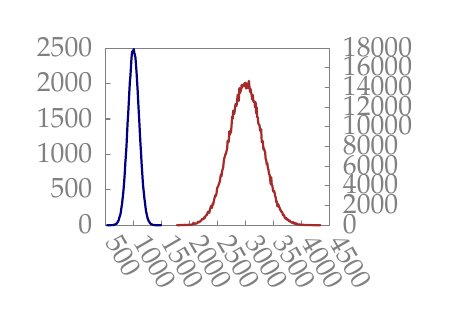
\begin{tikzpicture}[gnuplot, scale=0.3]
%% generated with GNUPLOT 5.2p2 (Lua 5.3; terminal rev. 99, script rev. 102)
%% wo 11 jul 2018 09:51:59 CEST
\path (0.000,0.000) rectangle (12.500,8.750);
\gpcolor{rgb color={0.502,0.502,0.502}}
\gpsetlinetype{gp lt border}
\gpsetdashtype{gp dt solid}
\gpsetlinewidth{1.00}
\draw[gp path] (1.196,0.945)--(1.376,0.945);
\node[gp node right] at (1.012,0.945) {$0$};
\draw[gp path] (1.196,2.444)--(1.376,2.444);
\node[gp node right] at (1.012,2.444) {$500$};
\draw[gp path] (1.196,3.943)--(1.376,3.943);
\node[gp node right] at (1.012,3.943) {$1000$};
\draw[gp path] (1.196,5.443)--(1.376,5.443);
\node[gp node right] at (1.012,5.443) {$1500$};
\draw[gp path] (1.196,6.942)--(1.376,6.942);
\node[gp node right] at (1.012,6.942) {$2000$};
\draw[gp path] (1.196,8.441)--(1.376,8.441);
\node[gp node right] at (1.012,8.441) {$2500$};
\draw[gp path] (1.196,0.945)--(1.196,1.125);
\node[gp node left,rotate=-60] at (1.196,0.761) {$500$};
\draw[gp path] (2.379,0.945)--(2.379,1.125);
\node[gp node left,rotate=-60] at (2.379,0.761) {$1000$};
\draw[gp path] (3.562,0.945)--(3.562,1.125);
\node[gp node left,rotate=-60] at (3.562,0.761) {$1500$};
\draw[gp path] (4.745,0.945)--(4.745,1.125);
\node[gp node left,rotate=-60] at (4.745,0.761) {$2000$};
\draw[gp path] (5.928,0.945)--(5.928,1.125);
\node[gp node left,rotate=-60] at (5.928,0.761) {$2500$};
\draw[gp path] (7.110,0.945)--(7.110,1.125);
\node[gp node left,rotate=-60] at (7.110,0.761) {$3000$};
\draw[gp path] (8.293,0.945)--(8.293,1.125);
\node[gp node left,rotate=-60] at (8.293,0.761) {$3500$};
\draw[gp path] (9.476,0.945)--(9.476,1.125);
\node[gp node left,rotate=-60] at (9.476,0.761) {$4000$};
\draw[gp path] (10.659,0.945)--(10.659,1.125);
\node[gp node left,rotate=-60] at (10.659,0.761) {$4500$};
\draw[gp path] (10.659,0.945)--(10.479,0.945);
\node[gp node left] at (10.843,0.945) {$0$};
\draw[gp path] (10.659,1.778)--(10.479,1.778);
\node[gp node left] at (10.843,1.778) {$2000$};
\draw[gp path] (10.659,2.611)--(10.479,2.611);
\node[gp node left] at (10.843,2.611) {$4000$};
\draw[gp path] (10.659,3.444)--(10.479,3.444);
\node[gp node left] at (10.843,3.444) {$6000$};
\draw[gp path] (10.659,4.277)--(10.479,4.277);
\node[gp node left] at (10.843,4.277) {$8000$};
\draw[gp path] (10.659,5.109)--(10.479,5.109);
\node[gp node left] at (10.843,5.109) {$10000$};
\draw[gp path] (10.659,5.942)--(10.479,5.942);
\node[gp node left] at (10.843,5.942) {$12000$};
\draw[gp path] (10.659,6.775)--(10.479,6.775);
\node[gp node left] at (10.843,6.775) {$14000$};
\draw[gp path] (10.659,7.608)--(10.479,7.608);
\node[gp node left] at (10.843,7.608) {$16000$};
\draw[gp path] (10.659,8.441)--(10.479,8.441);
\node[gp node left] at (10.843,8.441) {$18000$};
\draw[gp path] (1.196,8.441)--(1.196,0.945)--(10.659,0.945)--(10.659,8.441)--cycle;
\gpcolor{rgb color={0.647,0.165,0.165}}
\gpsetlinewidth{2.00}
\draw[gp path] (4.201,0.951)--(4.224,0.951)--(4.248,0.948)--(4.271,0.948)--(4.295,0.948)%
  --(4.319,0.948)--(4.342,0.948)--(4.366,0.954)--(4.390,0.948)--(4.413,0.954)--(4.461,0.948)%
  --(4.484,0.963)--(4.508,0.951)--(4.532,0.966)--(4.555,0.960)--(4.579,0.951)--(4.603,0.957)%
  --(4.626,0.957)--(4.650,0.960)--(4.674,0.963)--(4.697,0.957)--(4.721,0.978)--(4.745,0.960)%
  --(4.768,0.960)--(4.792,0.972)--(4.816,0.969)--(4.839,0.978)--(4.863,0.975)--(4.887,1.005)%
  --(4.910,1.050)--(4.934,1.008)--(4.958,1.002)--(4.981,1.023)--(5.005,1.011)--(5.029,1.026)%
  --(5.052,1.020)--(5.076,1.044)--(5.099,1.098)--(5.123,1.071)--(5.147,1.071)--(5.170,1.098)%
  --(5.194,1.098)--(5.218,1.146)--(5.241,1.143)--(5.265,1.206)--(5.289,1.215)--(5.312,1.200)%
  --(5.336,1.212)--(5.360,1.281)--(5.383,1.251)--(5.407,1.314)--(5.431,1.353)--(5.454,1.374)%
  --(5.478,1.371)--(5.502,1.470)--(5.525,1.521)--(5.549,1.500)--(5.573,1.467)--(5.596,1.560)%
  --(5.620,1.659)--(5.644,1.761)--(5.667,1.731)--(5.691,1.677)--(5.715,1.854)--(5.738,1.818)%
  --(5.762,1.928)--(5.786,2.051)--(5.809,2.135)--(5.833,2.216)--(5.857,2.189)--(5.880,2.276)%
  --(5.904,2.480)--(5.928,2.564)--(5.951,2.585)--(5.975,2.666)--(5.998,2.726)--(6.022,2.795)%
  --(6.046,2.969)--(6.069,3.095)--(6.093,3.017)--(6.117,3.224)--(6.140,3.317)--(6.164,3.380)%
  --(6.188,3.647)--(6.211,3.784)--(6.235,3.850)--(6.259,3.955)--(6.282,3.961)--(6.306,4.093)%
  --(6.330,4.168)--(6.353,4.519)--(6.377,4.471)--(6.401,4.483)--(6.424,4.930)--(6.448,4.777)%
  --(6.472,4.867)--(6.495,4.876)--(6.519,5.173)--(6.543,5.548)--(6.566,5.449)--(6.590,5.799)%
  --(6.614,5.646)--(6.637,5.682)--(6.661,5.856)--(6.685,6.066)--(6.708,6.039)--(6.732,6.006)%
  --(6.756,6.249)--(6.779,6.465)--(6.803,6.480)--(6.826,6.210)--(6.850,6.747)--(6.874,6.534)%
  --(6.897,6.609)--(6.921,6.654)--(6.945,6.882)--(6.968,6.777)--(6.992,6.876)--(7.016,6.888)%
  --(7.039,6.855)--(7.063,6.957)--(7.087,6.819)--(7.110,6.981)--(7.134,6.735)--(7.158,6.753)%
  --(7.181,6.933)--(7.205,6.771)--(7.229,6.753)--(7.252,7.056)--(7.276,6.825)--(7.300,6.591)%
  --(7.323,6.717)--(7.347,6.576)--(7.371,6.441)--(7.394,6.270)--(7.418,6.459)--(7.442,6.189)%
  --(7.465,6.159)--(7.489,6.186)--(7.513,5.934)--(7.536,6.159)--(7.560,5.679)--(7.584,5.940)%
  --(7.607,5.521)--(7.631,5.500)--(7.654,5.242)--(7.678,5.215)--(7.702,5.179)--(7.725,4.972)%
  --(7.749,4.930)--(7.773,5.005)--(7.796,4.480)--(7.820,4.459)--(7.844,4.501)--(7.867,4.162)%
  --(7.891,4.210)--(7.915,4.093)--(7.938,4.075)--(7.962,3.755)--(7.986,3.707)--(8.009,3.515)%
  --(8.033,3.575)--(8.057,3.362)--(8.080,3.305)--(8.104,3.116)--(8.128,3.086)--(8.151,2.915)%
  --(8.175,2.684)--(8.199,2.972)--(8.222,2.627)--(8.246,2.624)--(8.270,2.432)--(8.293,2.360)%
  --(8.317,2.402)--(8.341,2.327)--(8.364,2.174)--(8.388,2.120)--(8.412,1.928)--(8.435,1.961)%
  --(8.459,1.749)--(8.483,1.836)--(8.506,1.809)--(8.530,1.701)--(8.553,1.695)--(8.577,1.602)%
  --(8.601,1.578)--(8.624,1.518)--(8.648,1.509)--(8.672,1.485)--(8.695,1.368)--(8.719,1.398)%
  --(8.743,1.365)--(8.766,1.284)--(8.790,1.236)--(8.814,1.230)--(8.837,1.242)--(8.861,1.182)%
  --(8.885,1.209)--(8.908,1.161)--(8.932,1.155)--(8.956,1.116)--(8.979,1.146)--(9.003,1.116)%
  --(9.027,1.071)--(9.050,1.077)--(9.074,1.041)--(9.098,1.056)--(9.121,1.074)--(9.145,1.026)%
  --(9.169,1.020)--(9.192,1.050)--(9.216,0.999)--(9.240,1.014)--(9.263,1.029)--(9.287,0.999)%
  --(9.311,0.978)--(9.334,0.975)--(9.358,0.975)--(9.381,0.981)--(9.405,0.984)--(9.429,0.966)%
  --(9.452,0.957)--(9.476,0.969)--(9.500,0.966)--(9.523,0.963)--(9.547,0.960)--(9.571,0.963)%
  --(9.594,0.957)--(9.618,0.951)--(9.665,0.954)--(9.689,0.966)--(9.713,0.954)--(9.736,0.951)%
  --(9.760,0.960)--(9.784,0.954)--(9.831,0.948)--(9.855,0.951)--(9.997,0.948)--(10.044,0.948)%
  --(10.139,0.948)--(10.257,0.948)--(10.280,0.948);
\gpcolor{rgb color={0.000,0.000,0.502}}
\draw[gp path] (1.243,0.945)--(1.314,0.946)--(1.362,0.945)--(1.385,0.948)--(1.409,0.948)%
  --(1.433,0.950)--(1.456,0.950)--(1.480,0.949)--(1.504,0.954)--(1.527,0.958)--(1.551,0.971)%
  --(1.575,0.967)--(1.598,0.983)--(1.622,1.002)--(1.645,1.009)--(1.669,1.030)--(1.693,1.075)%
  --(1.716,1.106)--(1.740,1.161)--(1.764,1.249)--(1.787,1.328)--(1.811,1.388)--(1.835,1.523)%
  --(1.858,1.701)--(1.882,1.830)--(1.906,2.070)--(1.929,2.266)--(1.953,2.529)--(1.977,2.839)%
  --(2.000,3.188)--(2.024,3.606)--(2.048,3.941)--(2.071,4.295)--(2.095,4.804)--(2.119,5.306)%
  --(2.142,5.637)--(2.166,6.093)--(2.190,6.574)--(2.213,6.989)--(2.237,7.257)--(2.261,7.647)%
  --(2.284,8.031)--(2.308,8.290)--(2.332,8.311)--(2.355,8.322)--(2.379,8.399)--(2.403,8.237)%
  --(2.426,8.162)--(2.450,8.034)--(2.474,7.744)--(2.497,7.419)--(2.521,7.007)--(2.544,6.644)%
  --(2.568,6.165)--(2.592,5.709)--(2.615,5.319)--(2.639,4.826)--(2.663,4.386)--(2.686,4.030)%
  --(2.710,3.567)--(2.734,3.212)--(2.757,2.854)--(2.781,2.552)--(2.805,2.328)--(2.828,2.096)%
  --(2.852,1.913)--(2.876,1.718)--(2.899,1.534)--(2.923,1.428)--(2.947,1.316)--(2.970,1.222)%
  --(2.994,1.169)--(3.018,1.104)--(3.041,1.085)--(3.065,1.034)--(3.089,1.014)--(3.112,0.997)%
  --(3.136,0.991)--(3.160,0.970)--(3.183,0.960)--(3.207,0.960)--(3.231,0.952)--(3.254,0.952)%
  --(3.278,0.951)--(3.302,0.947)--(3.325,0.947)--(3.349,0.947)--(3.372,0.945)--(3.491,0.945)%
  --(3.538,0.945);
%% coordinates of the plot area
\gpdefrectangularnode{gp plot 1}{\pgfpoint{1.196cm}{0.945cm}}{\pgfpoint{10.659cm}{8.441cm}}
\end{tikzpicture}
%% gnuplot variables

\end{tabular}
\end{center}
\caption{\label{fig:inputselection:normal_3to1_largeThenRandom}
  Same distribution and ratio as in
  Figure~\ref{fig:inputselection:normal_3to1_largest}; we run the largest-first
  algorithm for 1M cycles, and then random coin selection for another 150k
  cycles.
}
\end{figure}

Notice quite how rapidly the random coin selection reduces the size of the UTxO
once it kicks in. If you look at the inputs-per-transaction histogram, you can see
that when the random input selection takes over, it first creates a bunch of
transactions with 10 inputs (we limited transaction size to 10 for this
simulation), rapidly collecting dust. Once the dust is gone, the number of
inputs shrinks to about 3 or 4, which makes perfect sense given the 3:1 ratio of
deposits and withdrawals.

We will restate Erhardt's observation as our first self organisation principle:
%
\begin{quote}
\textbf{Self organisation principle 1}. Random selection has a high probability
of picking dust outputs \emph{precisely when} there is a lot of dust in the UTxO.
\end{quote}
%
It provides a very promising starting point for an effective coin selection
algorithm, but there are some improvements we can make.

\subsection{Active UTxO management}

Figure~\ref{fig:inputselection:normal_1to1_randomOff} shows a simulation of a
pure ``select randomly until we reach the target value'' coin selection algorithm.
The first observation is that this algorithm is doing \emph{much} better than
the largest-first policy in terms of the size of the UTxO, which is about
\emph{2 orders of magnitude} smaller: a dramatic improvement. However, if we
look at the UTxO histogram, we can see that there is room for improvement:
although this algorithm is good at collecting dust, it's also still
\emph{generating} quite a bit of dust. The UTxO histogram has two peaks. The
first one is approximately normally distributed around 1000, which are the
deposits that are being made. The second one is near 0, which are all the dust
outputs that are being created.

\begin{figure}[p]
\begin{center}
\scriptsize
\begin{tabular}{ll}
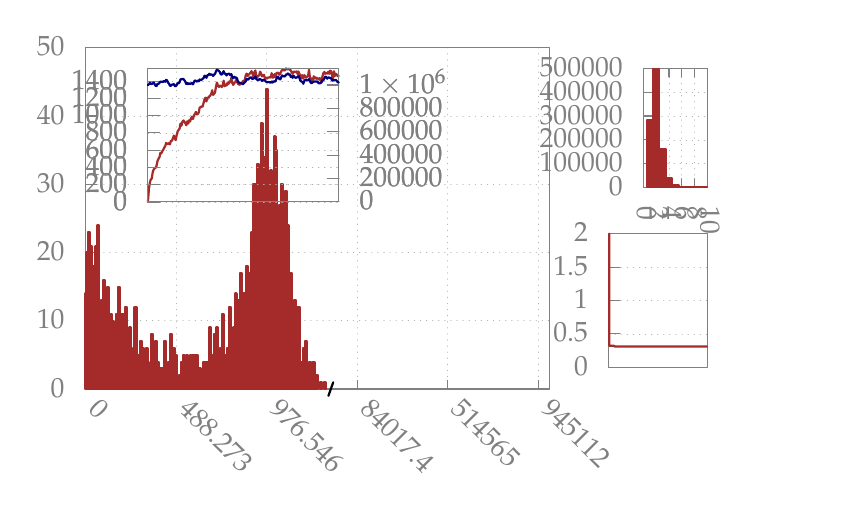
\begin{tikzpicture}[gnuplot, xscale=0.8, yscale=0.6]
%% generated with GNUPLOT 5.2p2 (Lua 5.3; terminal rev. 99, script rev. 102)
%% wo 11 jul 2018 10:29:34 CEST
\path (0.000,0.000) rectangle (12.500,8.750);
\gpcolor{color=gp lt color axes}
\gpsetlinetype{gp lt axes}
\gpsetdashtype{gp dt axes}
\gpsetlinewidth{0.50}
\draw[gp path] (0.828,1.218)--(8.197,1.218);
\gpcolor{rgb color={0.502,0.502,0.502}}
\gpsetlinetype{gp lt border}
\gpsetdashtype{gp dt solid}
\gpsetlinewidth{1.00}
\draw[gp path] (0.828,1.218)--(1.008,1.218);
\node[gp node right] at (0.644,1.218) {$0$};
\gpcolor{color=gp lt color axes}
\gpsetlinetype{gp lt axes}
\gpsetdashtype{gp dt axes}
\gpsetlinewidth{0.50}
\draw[gp path] (0.828,2.663)--(8.197,2.663);
\gpcolor{rgb color={0.502,0.502,0.502}}
\gpsetlinetype{gp lt border}
\gpsetdashtype{gp dt solid}
\gpsetlinewidth{1.00}
\draw[gp path] (0.828,2.663)--(1.008,2.663);
\node[gp node right] at (0.644,2.663) {$10$};
\gpcolor{color=gp lt color axes}
\gpsetlinetype{gp lt axes}
\gpsetdashtype{gp dt axes}
\gpsetlinewidth{0.50}
\draw[gp path] (0.828,4.107)--(8.197,4.107);
\gpcolor{rgb color={0.502,0.502,0.502}}
\gpsetlinetype{gp lt border}
\gpsetdashtype{gp dt solid}
\gpsetlinewidth{1.00}
\draw[gp path] (0.828,4.107)--(1.008,4.107);
\node[gp node right] at (0.644,4.107) {$20$};
\gpcolor{color=gp lt color axes}
\gpsetlinetype{gp lt axes}
\gpsetdashtype{gp dt axes}
\gpsetlinewidth{0.50}
\draw[gp path] (0.828,5.552)--(8.197,5.552);
\gpcolor{rgb color={0.502,0.502,0.502}}
\gpsetlinetype{gp lt border}
\gpsetdashtype{gp dt solid}
\gpsetlinewidth{1.00}
\draw[gp path] (0.828,5.552)--(1.008,5.552);
\node[gp node right] at (0.644,5.552) {$30$};
\gpcolor{color=gp lt color axes}
\gpsetlinetype{gp lt axes}
\gpsetdashtype{gp dt axes}
\gpsetlinewidth{0.50}
\draw[gp path] (0.828,6.996)--(8.197,6.996);
\gpcolor{rgb color={0.502,0.502,0.502}}
\gpsetlinetype{gp lt border}
\gpsetdashtype{gp dt solid}
\gpsetlinewidth{1.00}
\draw[gp path] (0.828,6.996)--(1.008,6.996);
\node[gp node right] at (0.644,6.996) {$40$};
\gpcolor{color=gp lt color axes}
\gpsetlinetype{gp lt axes}
\gpsetdashtype{gp dt axes}
\gpsetlinewidth{0.50}
\draw[gp path] (0.828,8.441)--(8.197,8.441);
\gpcolor{rgb color={0.502,0.502,0.502}}
\gpsetlinetype{gp lt border}
\gpsetdashtype{gp dt solid}
\gpsetlinewidth{1.00}
\draw[gp path] (0.828,8.441)--(1.008,8.441);
\node[gp node right] at (0.644,8.441) {$50$};
\gpcolor{color=gp lt color axes}
\gpsetlinetype{gp lt axes}
\gpsetdashtype{gp dt axes}
\gpsetlinewidth{0.50}
\draw[gp path] (0.828,1.218)--(0.828,8.441);
\gpcolor{rgb color={0.502,0.502,0.502}}
\gpsetlinetype{gp lt border}
\gpsetdashtype{gp dt solid}
\gpsetlinewidth{1.00}
\draw[gp path] (0.828,1.218)--(0.828,1.398);
\node[gp node left,rotate=-45] at (0.828,1.034) {$0$};
\gpcolor{color=gp lt color axes}
\gpsetlinetype{gp lt axes}
\gpsetdashtype{gp dt axes}
\gpsetlinewidth{0.50}
\draw[gp path] (2.266,1.218)--(2.266,8.441);
\gpcolor{rgb color={0.502,0.502,0.502}}
\gpsetlinetype{gp lt border}
\gpsetdashtype{gp dt solid}
\gpsetlinewidth{1.00}
\draw[gp path] (2.266,1.218)--(2.266,1.398);
\node[gp node left,rotate=-45] at (2.266,1.034) {$488.273$};
\gpcolor{color=gp lt color axes}
\gpsetlinetype{gp lt axes}
\gpsetdashtype{gp dt axes}
\gpsetlinewidth{0.50}
\draw[gp path] (3.704,1.218)--(3.704,8.441);
\gpcolor{rgb color={0.502,0.502,0.502}}
\gpsetlinetype{gp lt border}
\gpsetdashtype{gp dt solid}
\gpsetlinewidth{1.00}
\draw[gp path] (3.704,1.218)--(3.704,1.398);
\node[gp node left,rotate=-45] at (3.704,1.034) {$976.546$};
\gpcolor{color=gp lt color axes}
\gpsetlinetype{gp lt axes}
\gpsetdashtype{gp dt axes}
\gpsetlinewidth{0.50}
\draw[gp path] (5.142,1.218)--(5.142,8.441);
\gpcolor{rgb color={0.502,0.502,0.502}}
\gpsetlinetype{gp lt border}
\gpsetdashtype{gp dt solid}
\gpsetlinewidth{1.00}
\draw[gp path] (5.142,1.218)--(5.142,1.398);
\node[gp node left,rotate=-45] at (5.142,1.034) {$84017.4$};
\gpcolor{color=gp lt color axes}
\gpsetlinetype{gp lt axes}
\gpsetdashtype{gp dt axes}
\gpsetlinewidth{0.50}
\draw[gp path] (6.579,1.218)--(6.579,8.441);
\gpcolor{rgb color={0.502,0.502,0.502}}
\gpsetlinetype{gp lt border}
\gpsetdashtype{gp dt solid}
\gpsetlinewidth{1.00}
\draw[gp path] (6.579,1.218)--(6.579,1.398);
\node[gp node left,rotate=-45] at (6.579,1.034) {$514565$};
\gpcolor{color=gp lt color axes}
\gpsetlinetype{gp lt axes}
\gpsetdashtype{gp dt axes}
\gpsetlinewidth{0.50}
\draw[gp path] (8.017,1.218)--(8.017,8.441);
\gpcolor{rgb color={0.502,0.502,0.502}}
\gpsetlinetype{gp lt border}
\gpsetdashtype{gp dt solid}
\gpsetlinewidth{1.00}
\draw[gp path] (8.017,1.218)--(8.017,1.398);
\node[gp node left,rotate=-45] at (8.017,1.034) {$945112$};
\draw[gp path] (0.828,8.441)--(0.828,1.218)--(8.197,1.218)--(8.197,8.441)--cycle;
\gpcolor{rgb color={0.647,0.165,0.165}}
\gpsetlinewidth{2.00}
\draw[gp path] (0.828,1.218)--(0.828,3.240)--(0.843,3.240)--(0.843,1.218)--cycle;
\draw[gp path] (0.843,1.218)--(0.843,4.107)--(0.872,4.107)--(0.872,1.218)--cycle;
\draw[gp path] (0.872,1.218)--(0.872,4.541)--(0.902,4.541)--(0.902,1.218)--cycle;
\draw[gp path] (0.902,1.218)--(0.902,4.252)--(0.931,4.252)--(0.931,1.218)--cycle;
\draw[gp path] (0.931,1.218)--(0.931,3.818)--(0.961,3.818)--(0.961,1.218)--cycle;
\draw[gp path] (0.961,1.218)--(0.961,2.952)--(0.990,2.952)--(0.990,1.218)--cycle;
\draw[gp path] (0.990,1.218)--(0.990,4.252)--(1.019,4.252)--(1.019,1.218)--cycle;
\draw[gp path] (1.019,1.218)--(1.019,4.685)--(1.049,4.685)--(1.049,1.218)--cycle;
\draw[gp path] (1.049,1.218)--(1.049,2.518)--(1.078,2.518)--(1.078,1.218)--cycle;
\draw[gp path] (1.078,1.218)--(1.078,3.096)--(1.108,3.096)--(1.108,1.218)--cycle;
\draw[gp path] (1.108,1.218)--(1.108,3.529)--(1.137,3.529)--(1.137,1.218)--cycle;
\draw[gp path] (1.137,1.218)--(1.137,3.096)--(1.167,3.096)--(1.167,1.218)--cycle;
\draw[gp path] (1.167,1.218)--(1.167,3.385)--(1.196,3.385)--(1.196,1.218)--cycle;
\draw[gp path] (1.196,1.218)--(1.196,2.807)--(1.226,2.807)--(1.226,1.218)--cycle;
\draw[gp path] (1.226,1.218)--(1.226,2.807)--(1.255,2.807)--(1.255,1.218)--cycle;
\draw[gp path] (1.255,1.218)--(1.255,2.663)--(1.284,2.663)--(1.284,1.218)--cycle;
\draw[gp path] (1.284,1.218)--(1.284,2.518)--(1.314,2.518)--(1.314,1.218)--cycle;
\draw[gp path] (1.314,1.218)--(1.314,2.807)--(1.343,2.807)--(1.343,1.218)--cycle;
\draw[gp path] (1.343,1.218)--(1.343,3.385)--(1.373,3.385)--(1.373,1.218)--cycle;
\draw[gp path] (1.373,1.218)--(1.373,2.085)--(1.402,2.085)--(1.402,1.218)--cycle;
\draw[gp path] (1.402,1.218)--(1.402,2.807)--(1.432,2.807)--(1.432,1.218)--cycle;
\draw[gp path] (1.432,1.218)--(1.432,1.940)--(1.461,1.940)--(1.461,1.218)--cycle;
\draw[gp path] (1.461,1.218)--(1.461,2.952)--(1.491,2.952)--(1.491,1.218)--cycle;
\draw[gp path] (1.491,1.218)--(1.491,2.229)--(1.520,2.229)--(1.520,1.218)--cycle;
\draw[gp path] (1.520,1.218)--(1.520,2.518)--(1.549,2.518)--(1.549,1.218)--cycle;
\draw[gp path] (1.549,1.218)--(1.549,1.651)--(1.579,1.651)--(1.579,1.218)--cycle;
\draw[gp path] (1.579,1.218)--(1.579,2.085)--(1.608,2.085)--(1.608,1.218)--cycle;
\draw[gp path] (1.608,1.218)--(1.608,2.952)--(1.638,2.952)--(1.638,1.218)--cycle;
\draw[gp path] (1.638,1.218)--(1.638,1.940)--(1.667,1.940)--(1.667,1.218)--cycle;
\draw[gp path] (1.667,1.218)--(1.667,1.940)--(1.697,1.940)--(1.697,1.218)--cycle;
\draw[gp path] (1.697,1.218)--(1.697,2.229)--(1.726,2.229)--(1.726,1.218)--cycle;
\draw[gp path] (1.726,1.218)--(1.726,2.085)--(1.756,2.085)--(1.756,1.218)--cycle;
\draw[gp path] (1.756,1.218)--(1.756,1.940)--(1.785,1.940)--(1.785,1.218)--cycle;
\draw[gp path] (1.785,1.218)--(1.785,2.085)--(1.814,2.085)--(1.814,1.218)--cycle;
\draw[gp path] (1.814,1.218)--(1.814,1.796)--(1.844,1.796)--(1.844,1.218)--cycle;
\draw[gp path] (1.844,1.218)--(1.844,1.651)--(1.873,1.651)--(1.873,1.218)--cycle;
\draw[gp path] (1.873,1.218)--(1.873,2.374)--(1.903,2.374)--(1.903,1.218)--cycle;
\draw[gp path] (1.903,1.218)--(1.903,2.085)--(1.932,2.085)--(1.932,1.218)--cycle;
\draw[gp path] (1.932,1.218)--(1.932,2.229)--(1.962,2.229)--(1.962,1.218)--cycle;
\draw[gp path] (1.962,1.218)--(1.962,1.796)--(1.991,1.796)--(1.991,1.218)--cycle;
\draw[gp path] (1.991,1.218)--(1.991,1.507)--(2.021,1.507)--(2.021,1.218)--cycle;
\draw[gp path] (2.021,1.218)--(2.021,1.651)--(2.050,1.651)--(2.050,1.218)--cycle;
\draw[gp path] (2.050,1.218)--(2.050,1.651)--(2.080,1.651)--(2.080,1.218)--cycle;
\draw[gp path] (2.080,1.218)--(2.080,2.229)--(2.109,2.229)--(2.109,1.218)--cycle;
\draw[gp path] (2.109,1.218)--(2.109,1.507)--(2.138,1.507)--(2.138,1.218)--cycle;
\draw[gp path] (2.138,1.218)--(2.138,1.796)--(2.168,1.796)--(2.168,1.218)--cycle;
\draw[gp path] (2.168,1.218)--(2.168,2.374)--(2.197,2.374)--(2.197,1.218)--cycle;
\draw[gp path] (2.197,1.218)--(2.197,1.940)--(2.227,1.940)--(2.227,1.218)--cycle;
\draw[gp path] (2.227,1.218)--(2.227,2.085)--(2.256,2.085)--(2.256,1.218)--cycle;
\draw[gp path] (2.256,1.218)--(2.256,1.940)--(2.286,1.940)--(2.286,1.218)--cycle;
\draw[gp path] (2.286,1.218)--(2.286,1.362)--(2.315,1.362)--(2.315,1.218)--cycle;
\draw[gp path] (2.315,1.218)--(2.315,1.507)--(2.345,1.507)--(2.345,1.218)--cycle;
\draw[gp path] (2.345,1.218)--(2.345,1.796)--(2.374,1.796)--(2.374,1.218)--cycle;
\draw[gp path] (2.374,1.218)--(2.374,1.940)--(2.403,1.940)--(2.403,1.218)--cycle;
\draw[gp path] (2.403,1.218)--(2.403,1.651)--(2.433,1.651)--(2.433,1.218)--cycle;
\draw[gp path] (2.433,1.218)--(2.433,1.940)--(2.462,1.940)--(2.462,1.218)--cycle;
\draw[gp path] (2.462,1.218)--(2.462,1.651)--(2.492,1.651)--(2.492,1.218)--cycle;
\draw[gp path] (2.492,1.218)--(2.492,1.940)--(2.521,1.940)--(2.521,1.218)--cycle;
\draw[gp path] (2.521,1.218)--(2.521,1.940)--(2.551,1.940)--(2.551,1.218)--cycle;
\draw[gp path] (2.551,1.218)--(2.551,1.940)--(2.580,1.940)--(2.580,1.218)--cycle;
\draw[gp path] (2.580,1.218)--(2.580,1.940)--(2.610,1.940)--(2.610,1.218)--cycle;
\draw[gp path] (2.610,1.218)--(2.610,1.507)--(2.639,1.507)--(2.639,1.218)--cycle;
\draw[gp path] (2.639,1.218)--(2.639,1.651)--(2.668,1.651)--(2.668,1.218)--cycle;
\draw[gp path] (2.668,1.218)--(2.668,1.507)--(2.698,1.507)--(2.698,1.218)--cycle;
\draw[gp path] (2.698,1.218)--(2.698,1.796)--(2.727,1.796)--(2.727,1.218)--cycle;
\draw[gp path] (2.727,1.218)--(2.727,1.796)--(2.757,1.796)--(2.757,1.218)--cycle;
\draw[gp path] (2.757,1.218)--(2.757,1.796)--(2.786,1.796)--(2.786,1.218)--cycle;
\draw[gp path] (2.786,1.218)--(2.786,2.518)--(2.816,2.518)--(2.816,1.218)--cycle;
\draw[gp path] (2.816,1.218)--(2.816,1.651)--(2.845,1.651)--(2.845,1.218)--cycle;
\draw[gp path] (2.845,1.218)--(2.845,1.940)--(2.875,1.940)--(2.875,1.218)--cycle;
\draw[gp path] (2.875,1.218)--(2.875,2.374)--(2.904,2.374)--(2.904,1.218)--cycle;
\draw[gp path] (2.904,1.218)--(2.904,2.518)--(2.934,2.518)--(2.934,1.218)--cycle;
\draw[gp path] (2.934,1.218)--(2.934,1.507)--(2.963,1.507)--(2.963,1.218)--cycle;
\draw[gp path] (2.963,1.218)--(2.963,2.085)--(2.992,2.085)--(2.992,1.218)--cycle;
\draw[gp path] (2.992,1.218)--(2.992,2.807)--(3.022,2.807)--(3.022,1.218)--cycle;
\draw[gp path] (3.022,1.218)--(3.022,1.940)--(3.051,1.940)--(3.051,1.218)--cycle;
\draw[gp path] (3.051,1.218)--(3.051,1.507)--(3.081,1.507)--(3.081,1.218)--cycle;
\draw[gp path] (3.081,1.218)--(3.081,2.085)--(3.110,2.085)--(3.110,1.218)--cycle;
\draw[gp path] (3.110,1.218)--(3.110,2.952)--(3.140,2.952)--(3.140,1.218)--cycle;
\draw[gp path] (3.140,1.218)--(3.140,2.374)--(3.169,2.374)--(3.169,1.218)--cycle;
\draw[gp path] (3.169,1.218)--(3.169,2.518)--(3.199,2.518)--(3.199,1.218)--cycle;
\draw[gp path] (3.199,1.218)--(3.199,3.240)--(3.228,3.240)--(3.228,1.218)--cycle;
\draw[gp path] (3.228,1.218)--(3.228,2.518)--(3.257,2.518)--(3.257,1.218)--cycle;
\draw[gp path] (3.257,1.218)--(3.257,3.096)--(3.287,3.096)--(3.287,1.218)--cycle;
\draw[gp path] (3.287,1.218)--(3.287,3.674)--(3.316,3.674)--(3.316,1.218)--cycle;
\draw[gp path] (3.316,1.218)--(3.316,3.240)--(3.346,3.240)--(3.346,1.218)--cycle;
\draw[gp path] (3.346,1.218)--(3.346,3.240)--(3.375,3.240)--(3.375,1.218)--cycle;
\draw[gp path] (3.375,1.218)--(3.375,3.818)--(3.405,3.818)--(3.405,1.218)--cycle;
\draw[gp path] (3.405,1.218)--(3.405,3.674)--(3.434,3.674)--(3.434,1.218)--cycle;
\draw[gp path] (3.434,1.218)--(3.434,3.529)--(3.464,3.529)--(3.464,1.218)--cycle;
\draw[gp path] (3.464,1.218)--(3.464,4.541)--(3.493,4.541)--(3.493,1.218)--cycle;
\draw[gp path] (3.493,1.218)--(3.493,5.552)--(3.522,5.552)--(3.522,1.218)--cycle;
\draw[gp path] (3.522,1.218)--(3.522,5.552)--(3.552,5.552)--(3.552,1.218)--cycle;
\draw[gp path] (3.552,1.218)--(3.552,5.985)--(3.581,5.985)--(3.581,1.218)--cycle;
\draw[gp path] (3.581,1.218)--(3.581,5.263)--(3.611,5.263)--(3.611,1.218)--cycle;
\draw[gp path] (3.611,1.218)--(3.611,6.852)--(3.640,6.852)--(3.640,1.218)--cycle;
\draw[gp path] (3.640,1.218)--(3.640,5.985)--(3.670,5.985)--(3.670,1.218)--cycle;
\draw[gp path] (3.670,1.218)--(3.670,6.130)--(3.699,6.130)--(3.699,1.218)--cycle;
\draw[gp path] (3.699,1.218)--(3.699,7.574)--(3.729,7.574)--(3.729,1.218)--cycle;
\draw[gp path] (3.729,1.218)--(3.729,4.830)--(3.758,4.830)--(3.758,1.218)--cycle;
\draw[gp path] (3.758,1.218)--(3.758,5.841)--(3.787,5.841)--(3.787,1.218)--cycle;
\draw[gp path] (3.787,1.218)--(3.787,3.674)--(3.817,3.674)--(3.817,1.218)--cycle;
\draw[gp path] (3.817,1.218)--(3.817,6.563)--(3.846,6.563)--(3.846,1.218)--cycle;
\draw[gp path] (3.846,1.218)--(3.846,6.274)--(3.876,6.274)--(3.876,1.218)--cycle;
\draw[gp path] (3.876,1.218)--(3.876,4.252)--(3.905,4.252)--(3.905,1.218)--cycle;
\draw[gp path] (3.905,1.218)--(3.905,5.118)--(3.935,5.118)--(3.935,1.218)--cycle;
\draw[gp path] (3.935,1.218)--(3.935,5.552)--(3.964,5.552)--(3.964,1.218)--cycle;
\draw[gp path] (3.964,1.218)--(3.964,3.818)--(3.994,3.818)--(3.994,1.218)--cycle;
\draw[gp path] (3.994,1.218)--(3.994,5.407)--(4.023,5.407)--(4.023,1.218)--cycle;
\draw[gp path] (4.023,1.218)--(4.023,4.685)--(4.053,4.685)--(4.053,1.218)--cycle;
\draw[gp path] (4.053,1.218)--(4.053,2.952)--(4.082,2.952)--(4.082,1.218)--cycle;
\draw[gp path] (4.082,1.218)--(4.082,3.674)--(4.111,3.674)--(4.111,1.218)--cycle;
\draw[gp path] (4.111,1.218)--(4.111,2.663)--(4.141,2.663)--(4.141,1.218)--cycle;
\draw[gp path] (4.141,1.218)--(4.141,3.096)--(4.170,3.096)--(4.170,1.218)--cycle;
\draw[gp path] (4.170,1.218)--(4.170,2.952)--(4.200,2.952)--(4.200,1.218)--cycle;
\draw[gp path] (4.200,1.218)--(4.200,2.952)--(4.229,2.952)--(4.229,1.218)--cycle;
\draw[gp path] (4.229,1.218)--(4.229,1.796)--(4.259,1.796)--(4.259,1.218)--cycle;
\draw[gp path] (4.259,1.218)--(4.259,1.651)--(4.288,1.651)--(4.288,1.218)--cycle;
\draw[gp path] (4.288,1.218)--(4.288,2.085)--(4.318,2.085)--(4.318,1.218)--cycle;
\draw[gp path] (4.318,1.218)--(4.318,2.229)--(4.347,2.229)--(4.347,1.218)--cycle;
\draw[gp path] (4.347,1.218)--(4.347,1.362)--(4.376,1.362)--(4.376,1.218)--cycle;
\draw[gp path] (4.376,1.218)--(4.376,1.796)--(4.406,1.796)--(4.406,1.218)--cycle;
\draw[gp path] (4.406,1.218)--(4.406,1.651)--(4.435,1.651)--(4.435,1.218)--cycle;
\draw[gp path] (4.435,1.218)--(4.435,1.796)--(4.465,1.796)--(4.465,1.218)--cycle;
\draw[gp path] (4.465,1.218)--(4.465,1.507)--(4.494,1.507)--(4.494,1.218)--cycle;
\draw[gp path] (4.494,1.218)--(4.494,1.507)--(4.524,1.507)--(4.524,1.218)--cycle;
\draw[gp path] (4.553,1.218)--(4.553,1.362)--(4.583,1.362)--(4.583,1.218)--cycle;
\draw[gp path] (4.612,1.218)--(4.612,1.362)--(4.641,1.362)--(4.641,1.218)--cycle;
\gpcolor{color=gp lt color border}
\draw[gp path](4.686,1.074)--(4.762,1.358);
%% coordinates of the plot area
\gpdefrectangularnode{gp plot 1}{\pgfpoint{0.828cm}{1.218cm}}{\pgfpoint{8.197cm}{8.441cm}}
\gpcolor{color=gp lt color axes}
\gpsetlinetype{gp lt axes}
\gpsetdashtype{gp dt axes}
\gpsetlinewidth{0.50}
\draw[gp path] (1.821,5.176)--(4.850,5.176);
\gpcolor{rgb color={0.502,0.502,0.502}}
\gpsetlinetype{gp lt border}
\gpsetdashtype{gp dt solid}
\gpsetlinewidth{1.00}
\draw[gp path] (1.821,5.176)--(2.001,5.176);
\node[gp node right] at (1.637,5.176) {$0$};
\gpcolor{color=gp lt color axes}
\gpsetlinetype{gp lt axes}
\gpsetdashtype{gp dt axes}
\gpsetlinewidth{0.50}
\draw[gp path] (1.821,5.542)--(4.850,5.542);
\gpcolor{rgb color={0.502,0.502,0.502}}
\gpsetlinetype{gp lt border}
\gpsetdashtype{gp dt solid}
\gpsetlinewidth{1.00}
\draw[gp path] (1.821,5.542)--(2.001,5.542);
\node[gp node right] at (1.637,5.542) {$200$};
\gpcolor{color=gp lt color axes}
\gpsetlinetype{gp lt axes}
\gpsetdashtype{gp dt axes}
\gpsetlinewidth{0.50}
\draw[gp path] (1.821,5.907)--(4.850,5.907);
\gpcolor{rgb color={0.502,0.502,0.502}}
\gpsetlinetype{gp lt border}
\gpsetdashtype{gp dt solid}
\gpsetlinewidth{1.00}
\draw[gp path] (1.821,5.907)--(2.001,5.907);
\node[gp node right] at (1.637,5.907) {$400$};
\gpcolor{color=gp lt color axes}
\gpsetlinetype{gp lt axes}
\gpsetdashtype{gp dt axes}
\gpsetlinewidth{0.50}
\draw[gp path] (1.821,6.273)--(4.850,6.273);
\gpcolor{rgb color={0.502,0.502,0.502}}
\gpsetlinetype{gp lt border}
\gpsetdashtype{gp dt solid}
\gpsetlinewidth{1.00}
\draw[gp path] (1.821,6.273)--(2.001,6.273);
\node[gp node right] at (1.637,6.273) {$600$};
\gpcolor{color=gp lt color axes}
\gpsetlinetype{gp lt axes}
\gpsetdashtype{gp dt axes}
\gpsetlinewidth{0.50}
\draw[gp path] (1.821,6.639)--(4.850,6.639);
\gpcolor{rgb color={0.502,0.502,0.502}}
\gpsetlinetype{gp lt border}
\gpsetdashtype{gp dt solid}
\gpsetlinewidth{1.00}
\draw[gp path] (1.821,6.639)--(2.001,6.639);
\node[gp node right] at (1.637,6.639) {$800$};
\gpcolor{color=gp lt color axes}
\gpsetlinetype{gp lt axes}
\gpsetdashtype{gp dt axes}
\gpsetlinewidth{0.50}
\draw[gp path] (1.821,7.004)--(4.850,7.004);
\gpcolor{rgb color={0.502,0.502,0.502}}
\gpsetlinetype{gp lt border}
\gpsetdashtype{gp dt solid}
\gpsetlinewidth{1.00}
\draw[gp path] (1.821,7.004)--(2.001,7.004);
\node[gp node right] at (1.637,7.004) {$1000$};
\gpcolor{color=gp lt color axes}
\gpsetlinetype{gp lt axes}
\gpsetdashtype{gp dt axes}
\gpsetlinewidth{0.50}
\draw[gp path] (1.821,7.370)--(4.850,7.370);
\gpcolor{rgb color={0.502,0.502,0.502}}
\gpsetlinetype{gp lt border}
\gpsetdashtype{gp dt solid}
\gpsetlinewidth{1.00}
\draw[gp path] (1.821,7.370)--(2.001,7.370);
\node[gp node right] at (1.637,7.370) {$1200$};
\gpcolor{color=gp lt color axes}
\gpsetlinetype{gp lt axes}
\gpsetdashtype{gp dt axes}
\gpsetlinewidth{0.50}
\draw[gp path] (1.821,7.735)--(4.850,7.735);
\gpcolor{rgb color={0.502,0.502,0.502}}
\gpsetlinetype{gp lt border}
\gpsetdashtype{gp dt solid}
\gpsetlinewidth{1.00}
\draw[gp path] (1.821,7.735)--(2.001,7.735);
\node[gp node right] at (1.637,7.735) {$1400$};
\draw[gp path] (4.850,5.180)--(4.670,5.180);
\node[gp node left] at (5.034,5.180) {$0$};
\draw[gp path] (4.850,5.674)--(4.670,5.674);
\node[gp node left] at (5.034,5.674) {$200000$};
\draw[gp path] (4.850,6.169)--(4.670,6.169);
\node[gp node left] at (5.034,6.169) {$400000$};
\draw[gp path] (4.850,6.663)--(4.670,6.663);
\node[gp node left] at (5.034,6.663) {$600000$};
\draw[gp path] (4.850,7.157)--(4.670,7.157);
\node[gp node left] at (5.034,7.157) {$800000$};
\draw[gp path] (4.850,7.652)--(4.670,7.652);
\node[gp node left] at (5.034,7.652) {$1\times10^{6}$};
\draw[gp path] (1.821,8.004)--(1.821,5.180)--(4.850,5.180)--(4.850,8.004)--cycle;
\gpcolor{rgb color={0.647,0.165,0.165}}
\gpsetlinewidth{2.00}
\draw[gp path] (1.821,5.180)--(1.836,5.441)--(1.851,5.586)--(1.867,5.655)--(1.882,5.675)%
  --(1.897,5.807)--(1.912,5.864)--(1.928,5.889)--(1.943,5.900)--(1.958,5.946)--(1.973,6.045)%
  --(1.988,6.088)--(2.004,6.125)--(2.019,6.216)--(2.034,6.207)--(2.049,6.253)--(2.065,6.282)%
  --(2.080,6.330)--(2.095,6.355)--(2.110,6.427)--(2.125,6.408)--(2.141,6.399)--(2.156,6.423)%
  --(2.171,6.396)--(2.186,6.474)--(2.202,6.469)--(2.217,6.523)--(2.232,6.582)--(2.247,6.523)%
  --(2.262,6.485)--(2.278,6.597)--(2.293,6.672)--(2.308,6.701)--(2.323,6.730)--(2.339,6.838)%
  --(2.354,6.792)--(2.369,6.878)--(2.384,6.902)--(2.399,6.880)--(2.415,6.840)--(2.430,6.801)%
  --(2.445,6.884)--(2.460,6.836)--(2.476,6.907)--(2.491,6.880)--(2.506,6.953)--(2.521,6.975)%
  --(2.536,6.933)--(2.552,7.010)--(2.567,7.037)--(2.582,7.083)--(2.597,7.033)--(2.612,7.039)%
  --(2.628,7.070)--(2.643,7.181)--(2.658,7.178)--(2.673,7.202)--(2.689,7.196)--(2.704,7.271)%
  --(2.719,7.346)--(2.734,7.384)--(2.749,7.304)--(2.765,7.383)--(2.780,7.372)--(2.795,7.415)%
  --(2.810,7.428)--(2.826,7.467)--(2.841,7.540)--(2.856,7.441)--(2.871,7.472)--(2.886,7.490)%
  --(2.902,7.626)--(2.917,7.704)--(2.932,7.640)--(2.947,7.611)--(2.963,7.637)--(2.978,7.635)%
  --(2.993,7.609)--(3.008,7.644)--(3.023,7.744)--(3.039,7.626)--(3.054,7.664)--(3.069,7.640)%
  --(3.084,7.699)--(3.100,7.673)--(3.115,7.728)--(3.130,7.715)--(3.145,7.805)--(3.160,7.695)%
  --(3.176,7.655)--(3.191,7.697)--(3.206,7.710)--(3.221,7.761)--(3.237,7.713)--(3.252,7.677)%
  --(3.267,7.662)--(3.282,7.659)--(3.297,7.697)--(3.313,7.699)--(3.328,7.733)--(3.343,7.743)%
  --(3.358,7.757)--(3.374,7.861)--(3.389,7.894)--(3.404,7.843)--(3.419,7.869)--(3.434,7.889)%
  --(3.450,7.913)--(3.465,7.946)--(3.480,7.898)--(3.495,7.825)--(3.511,7.924)--(3.526,7.960)%
  --(3.541,7.843)--(3.556,7.821)--(3.571,7.841)--(3.587,7.860)--(3.602,7.936)--(3.617,7.894)%
  --(3.632,7.834)--(3.648,7.858)--(3.663,7.869)--(3.678,7.785)--(3.693,7.808)--(3.708,7.788)%
  --(3.724,7.810)--(3.739,7.808)--(3.754,7.818)--(3.769,7.812)--(3.785,7.902)--(3.800,7.807)%
  --(3.815,7.814)--(3.830,7.882)--(3.845,7.812)--(3.861,7.903)--(3.876,7.913)--(3.891,7.907)%
  --(3.906,7.869)--(3.922,7.893)--(3.937,7.942)--(3.952,7.973)--(3.967,7.978)--(3.982,7.958)%
  --(3.998,7.969)--(4.013,8.004)--(4.028,7.982)--(4.043,7.991)--(4.059,7.995)--(4.074,7.973)%
  --(4.089,7.964)--(4.104,7.918)--(4.119,7.889)--(4.135,7.933)--(4.150,7.936)--(4.165,7.924)%
  --(4.180,7.940)--(4.195,7.889)--(4.211,7.938)--(4.226,7.880)--(4.241,7.865)--(4.256,7.788)%
  --(4.272,7.861)--(4.287,7.785)--(4.302,7.861)--(4.317,7.841)--(4.332,7.812)--(4.348,7.827)%
  --(4.363,7.847)--(4.378,7.975)--(4.393,7.805)--(4.409,7.799)--(4.424,7.721)--(4.439,7.766)%
  --(4.454,7.838)--(4.469,7.788)--(4.485,7.814)--(4.500,7.785)--(4.515,7.799)--(4.530,7.774)%
  --(4.546,7.799)--(4.561,7.741)--(4.576,7.766)--(4.591,7.832)--(4.606,7.903)--(4.622,7.929)%
  --(4.637,7.889)--(4.652,7.907)--(4.667,7.894)--(4.683,7.931)--(4.698,7.889)--(4.713,7.955)%
  --(4.728,7.946)--(4.743,7.861)--(4.759,7.786)--(4.774,7.944)--(4.789,7.843)--(4.804,7.889)%
  --(4.820,7.871)--(4.835,7.836)--(4.850,7.845);
%% coordinates of the plot area
\gpdefrectangularnode{gp plot 2}{\pgfpoint{1.821cm}{5.180cm}}{\pgfpoint{4.850cm}{8.004cm}}
\gpcolor{color=gp lt color axes}
\gpsetlinetype{gp lt axes}
\gpsetdashtype{gp dt axes}
\gpsetlinewidth{0.50}
\draw[gp path] (1.821,5.176)--(4.850,5.176);
\gpcolor{rgb color={0.502,0.502,0.502}}
\gpsetlinetype{gp lt border}
\gpsetdashtype{gp dt solid}
\gpsetlinewidth{1.00}
\draw[gp path] (1.821,5.176)--(2.001,5.176);
\node[gp node right] at (1.637,5.176) {$0$};
\gpcolor{color=gp lt color axes}
\gpsetlinetype{gp lt axes}
\gpsetdashtype{gp dt axes}
\gpsetlinewidth{0.50}
\draw[gp path] (1.821,5.542)--(4.850,5.542);
\gpcolor{rgb color={0.502,0.502,0.502}}
\gpsetlinetype{gp lt border}
\gpsetdashtype{gp dt solid}
\gpsetlinewidth{1.00}
\draw[gp path] (1.821,5.542)--(2.001,5.542);
\node[gp node right] at (1.637,5.542) {$200$};
\gpcolor{color=gp lt color axes}
\gpsetlinetype{gp lt axes}
\gpsetdashtype{gp dt axes}
\gpsetlinewidth{0.50}
\draw[gp path] (1.821,5.907)--(4.850,5.907);
\gpcolor{rgb color={0.502,0.502,0.502}}
\gpsetlinetype{gp lt border}
\gpsetdashtype{gp dt solid}
\gpsetlinewidth{1.00}
\draw[gp path] (1.821,5.907)--(2.001,5.907);
\node[gp node right] at (1.637,5.907) {$400$};
\gpcolor{color=gp lt color axes}
\gpsetlinetype{gp lt axes}
\gpsetdashtype{gp dt axes}
\gpsetlinewidth{0.50}
\draw[gp path] (1.821,6.273)--(4.850,6.273);
\gpcolor{rgb color={0.502,0.502,0.502}}
\gpsetlinetype{gp lt border}
\gpsetdashtype{gp dt solid}
\gpsetlinewidth{1.00}
\draw[gp path] (1.821,6.273)--(2.001,6.273);
\node[gp node right] at (1.637,6.273) {$600$};
\gpcolor{color=gp lt color axes}
\gpsetlinetype{gp lt axes}
\gpsetdashtype{gp dt axes}
\gpsetlinewidth{0.50}
\draw[gp path] (1.821,6.639)--(4.850,6.639);
\gpcolor{rgb color={0.502,0.502,0.502}}
\gpsetlinetype{gp lt border}
\gpsetdashtype{gp dt solid}
\gpsetlinewidth{1.00}
\draw[gp path] (1.821,6.639)--(2.001,6.639);
\node[gp node right] at (1.637,6.639) {$800$};
\gpcolor{color=gp lt color axes}
\gpsetlinetype{gp lt axes}
\gpsetdashtype{gp dt axes}
\gpsetlinewidth{0.50}
\draw[gp path] (1.821,7.004)--(4.850,7.004);
\gpcolor{rgb color={0.502,0.502,0.502}}
\gpsetlinetype{gp lt border}
\gpsetdashtype{gp dt solid}
\gpsetlinewidth{1.00}
\draw[gp path] (1.821,7.004)--(2.001,7.004);
\node[gp node right] at (1.637,7.004) {$1000$};
\gpcolor{color=gp lt color axes}
\gpsetlinetype{gp lt axes}
\gpsetdashtype{gp dt axes}
\gpsetlinewidth{0.50}
\draw[gp path] (1.821,7.370)--(4.850,7.370);
\gpcolor{rgb color={0.502,0.502,0.502}}
\gpsetlinetype{gp lt border}
\gpsetdashtype{gp dt solid}
\gpsetlinewidth{1.00}
\draw[gp path] (1.821,7.370)--(2.001,7.370);
\node[gp node right] at (1.637,7.370) {$1200$};
\gpcolor{color=gp lt color axes}
\gpsetlinetype{gp lt axes}
\gpsetdashtype{gp dt axes}
\gpsetlinewidth{0.50}
\draw[gp path] (1.821,7.735)--(4.850,7.735);
\gpcolor{rgb color={0.502,0.502,0.502}}
\gpsetlinetype{gp lt border}
\gpsetdashtype{gp dt solid}
\gpsetlinewidth{1.00}
\draw[gp path] (1.821,7.735)--(2.001,7.735);
\node[gp node right] at (1.637,7.735) {$1400$};
\draw[gp path] (4.850,5.180)--(4.670,5.180);
\node[gp node left] at (5.034,5.180) {$0$};
\draw[gp path] (4.850,5.674)--(4.670,5.674);
\node[gp node left] at (5.034,5.674) {$200000$};
\draw[gp path] (4.850,6.169)--(4.670,6.169);
\node[gp node left] at (5.034,6.169) {$400000$};
\draw[gp path] (4.850,6.663)--(4.670,6.663);
\node[gp node left] at (5.034,6.663) {$600000$};
\draw[gp path] (4.850,7.157)--(4.670,7.157);
\node[gp node left] at (5.034,7.157) {$800000$};
\draw[gp path] (4.850,7.652)--(4.670,7.652);
\node[gp node left] at (5.034,7.652) {$1\times10^{6}$};
\draw[gp path] (1.821,8.004)--(1.821,5.180)--(4.850,5.180)--(4.850,8.004)--cycle;
\gpcolor{rgb color={0.000,0.000,0.502}}
\gpsetlinewidth{2.00}
\draw[gp path] (1.821,7.651)--(1.836,7.667)--(1.851,7.697)--(1.867,7.679)--(1.882,7.674)%
  --(1.897,7.688)--(1.912,7.704)--(1.928,7.670)--(1.943,7.637)--(1.958,7.629)--(1.973,7.678)%
  --(1.988,7.674)--(2.004,7.699)--(2.019,7.724)--(2.034,7.719)--(2.049,7.721)--(2.065,7.722)%
  --(2.080,7.741)--(2.095,7.722)--(2.110,7.762)--(2.125,7.750)--(2.141,7.700)--(2.156,7.681)%
  --(2.171,7.633)--(2.186,7.639)--(2.202,7.661)--(2.217,7.662)--(2.232,7.672)--(2.247,7.630)%
  --(2.262,7.628)--(2.278,7.651)--(2.293,7.698)--(2.308,7.685)--(2.323,7.710)--(2.339,7.774)%
  --(2.354,7.772)--(2.369,7.782)--(2.384,7.780)--(2.399,7.753)--(2.415,7.723)--(2.430,7.673)%
  --(2.445,7.697)--(2.460,7.671)--(2.476,7.692)--(2.491,7.675)--(2.506,7.685)--(2.521,7.693)%
  --(2.536,7.666)--(2.552,7.718)--(2.567,7.750)--(2.582,7.738)--(2.597,7.723)--(2.612,7.747)%
  --(2.628,7.732)--(2.643,7.769)--(2.658,7.753)--(2.673,7.766)--(2.689,7.783)--(2.704,7.798)%
  --(2.719,7.848)--(2.734,7.844)--(2.749,7.805)--(2.765,7.861)--(2.780,7.859)--(2.795,7.889)%
  --(2.810,7.868)--(2.826,7.877)--(2.841,7.868)--(2.856,7.845)--(2.871,7.874)--(2.886,7.886)%
  --(2.902,7.944)--(2.917,7.976)--(2.932,7.963)--(2.947,7.952)--(2.963,7.924)--(2.978,7.878)%
  --(2.993,7.873)--(3.008,7.906)--(3.023,7.945)--(3.039,7.887)--(3.054,7.894)--(3.069,7.855)%
  --(3.084,7.883)--(3.100,7.889)--(3.115,7.890)--(3.130,7.859)--(3.145,7.882)--(3.160,7.825)%
  --(3.176,7.797)--(3.191,7.827)--(3.206,7.803)--(3.221,7.816)--(3.237,7.783)--(3.252,7.717)%
  --(3.267,7.703)--(3.282,7.694)--(3.297,7.694)--(3.313,7.681)--(3.328,7.667)--(3.343,7.693)%
  --(3.358,7.708)--(3.374,7.734)--(3.389,7.780)--(3.404,7.761)--(3.419,7.780)--(3.434,7.798)%
  --(3.450,7.819)--(3.465,7.803)--(3.480,7.778)--(3.495,7.790)--(3.511,7.798)--(3.526,7.831)%
  --(3.541,7.781)--(3.556,7.765)--(3.571,7.751)--(3.587,7.775)--(3.602,7.774)--(3.617,7.766)%
  --(3.632,7.739)--(3.648,7.758)--(3.663,7.761)--(3.678,7.750)--(3.693,7.725)--(3.708,7.711)%
  --(3.724,7.712)--(3.739,7.715)--(3.754,7.710)--(3.769,7.700)--(3.785,7.725)--(3.800,7.706)%
  --(3.815,7.733)--(3.830,7.721)--(3.845,7.733)--(3.861,7.778)--(3.876,7.827)--(3.891,7.820)%
  --(3.906,7.783)--(3.922,7.771)--(3.937,7.817)--(3.952,7.855)--(3.967,7.840)--(3.982,7.834)%
  --(3.998,7.836)--(4.013,7.872)--(4.028,7.877)--(4.043,7.896)--(4.059,7.869)--(4.074,7.877)%
  --(4.089,7.823)--(4.104,7.841)--(4.119,7.805)--(4.135,7.847)--(4.150,7.820)--(4.165,7.806)%
  --(4.180,7.809)--(4.195,7.821)--(4.211,7.845)--(4.226,7.805)--(4.241,7.742)--(4.256,7.728)%
  --(4.272,7.719)--(4.287,7.680)--(4.302,7.733)--(4.317,7.760)--(4.332,7.765)--(4.348,7.750)%
  --(4.363,7.754)--(4.378,7.776)--(4.393,7.734)--(4.409,7.692)--(4.424,7.698)--(4.439,7.712)%
  --(4.454,7.722)--(4.469,7.727)--(4.485,7.728)--(4.500,7.723)--(4.515,7.725)--(4.530,7.688)%
  --(4.546,7.687)--(4.561,7.694)--(4.576,7.708)--(4.591,7.750)--(4.606,7.753)--(4.622,7.801)%
  --(4.637,7.831)--(4.652,7.820)--(4.667,7.786)--(4.683,7.810)--(4.698,7.810)--(4.713,7.802)%
  --(4.728,7.803)--(4.743,7.751)--(4.759,7.747)--(4.774,7.755)--(4.789,7.755)--(4.804,7.757)%
  --(4.820,7.738)--(4.835,7.711)--(4.850,7.707);
\gpcolor{color=gp lt color axes}
\gpsetlinetype{gp lt axes}
\gpsetdashtype{gp dt axes}
\gpsetlinewidth{0.50}
\draw[gp path] (9.688,5.488)--(10.697,5.488);
\gpcolor{rgb color={0.502,0.502,0.502}}
\gpsetlinetype{gp lt border}
\gpsetdashtype{gp dt solid}
\gpsetlinewidth{1.00}
\draw[gp path] (9.688,5.488)--(9.868,5.488);
\node[gp node right] at (9.504,5.488) {$0$};
\gpcolor{color=gp lt color axes}
\gpsetlinetype{gp lt axes}
\gpsetdashtype{gp dt axes}
\gpsetlinewidth{0.50}
\draw[gp path] (9.688,5.991)--(10.697,5.991);
\gpcolor{rgb color={0.502,0.502,0.502}}
\gpsetlinetype{gp lt border}
\gpsetdashtype{gp dt solid}
\gpsetlinewidth{1.00}
\draw[gp path] (9.688,5.991)--(9.868,5.991);
\node[gp node right] at (9.504,5.991) {$100000$};
\gpcolor{color=gp lt color axes}
\gpsetlinetype{gp lt axes}
\gpsetdashtype{gp dt axes}
\gpsetlinewidth{0.50}
\draw[gp path] (9.688,6.493)--(10.697,6.493);
\gpcolor{rgb color={0.502,0.502,0.502}}
\gpsetlinetype{gp lt border}
\gpsetdashtype{gp dt solid}
\gpsetlinewidth{1.00}
\draw[gp path] (9.688,6.493)--(9.868,6.493);
\node[gp node right] at (9.504,6.493) {$200000$};
\gpcolor{color=gp lt color axes}
\gpsetlinetype{gp lt axes}
\gpsetdashtype{gp dt axes}
\gpsetlinewidth{0.50}
\draw[gp path] (9.688,6.996)--(10.697,6.996);
\gpcolor{rgb color={0.502,0.502,0.502}}
\gpsetlinetype{gp lt border}
\gpsetdashtype{gp dt solid}
\gpsetlinewidth{1.00}
\draw[gp path] (9.688,6.996)--(9.868,6.996);
\node[gp node right] at (9.504,6.996) {$300000$};
\gpcolor{color=gp lt color axes}
\gpsetlinetype{gp lt axes}
\gpsetdashtype{gp dt axes}
\gpsetlinewidth{0.50}
\draw[gp path] (9.688,7.498)--(10.697,7.498);
\gpcolor{rgb color={0.502,0.502,0.502}}
\gpsetlinetype{gp lt border}
\gpsetdashtype{gp dt solid}
\gpsetlinewidth{1.00}
\draw[gp path] (9.688,7.498)--(9.868,7.498);
\node[gp node right] at (9.504,7.498) {$400000$};
\gpcolor{color=gp lt color axes}
\gpsetlinetype{gp lt axes}
\gpsetdashtype{gp dt axes}
\gpsetlinewidth{0.50}
\draw[gp path] (9.688,8.001)--(10.697,8.001);
\gpcolor{rgb color={0.502,0.502,0.502}}
\gpsetlinetype{gp lt border}
\gpsetdashtype{gp dt solid}
\gpsetlinewidth{1.00}
\draw[gp path] (9.688,8.001)--(9.868,8.001);
\node[gp node right] at (9.504,8.001) {$500000$};
\gpcolor{color=gp lt color axes}
\gpsetlinetype{gp lt axes}
\gpsetdashtype{gp dt axes}
\gpsetlinewidth{0.50}
\draw[gp path] (9.688,5.488)--(9.688,7.824)--(9.688,8.004);
\gpcolor{rgb color={0.502,0.502,0.502}}
\gpsetlinetype{gp lt border}
\gpsetdashtype{gp dt solid}
\gpsetlinewidth{1.00}
\draw[gp path] (9.688,5.488)--(9.688,5.668);
\draw[gp path] (9.688,8.004)--(9.688,7.824);
\node[gp node left,rotate=-90] at (9.688,5.304) {$0$};
\gpcolor{color=gp lt color axes}
\gpsetlinetype{gp lt axes}
\gpsetdashtype{gp dt axes}
\gpsetlinewidth{0.50}
\draw[gp path] (9.890,5.488)--(9.890,7.824)--(9.890,8.004);
\gpcolor{rgb color={0.502,0.502,0.502}}
\gpsetlinetype{gp lt border}
\gpsetdashtype{gp dt solid}
\gpsetlinewidth{1.00}
\draw[gp path] (9.890,5.488)--(9.890,5.668);
\draw[gp path] (9.890,8.004)--(9.890,7.824);
\node[gp node left,rotate=-90] at (9.890,5.304) {$2$};
\gpcolor{color=gp lt color axes}
\gpsetlinetype{gp lt axes}
\gpsetdashtype{gp dt axes}
\gpsetlinewidth{0.50}
\draw[gp path] (10.092,5.488)--(10.092,7.824)--(10.092,8.004);
\gpcolor{rgb color={0.502,0.502,0.502}}
\gpsetlinetype{gp lt border}
\gpsetdashtype{gp dt solid}
\gpsetlinewidth{1.00}
\draw[gp path] (10.092,5.488)--(10.092,5.668);
\draw[gp path] (10.092,8.004)--(10.092,7.824);
\node[gp node left,rotate=-90] at (10.092,5.304) {$4$};
\gpcolor{color=gp lt color axes}
\gpsetlinetype{gp lt axes}
\gpsetdashtype{gp dt axes}
\gpsetlinewidth{0.50}
\draw[gp path] (10.293,5.488)--(10.293,7.824)--(10.293,8.004);
\gpcolor{rgb color={0.502,0.502,0.502}}
\gpsetlinetype{gp lt border}
\gpsetdashtype{gp dt solid}
\gpsetlinewidth{1.00}
\draw[gp path] (10.293,5.488)--(10.293,5.668);
\draw[gp path] (10.293,8.004)--(10.293,7.824);
\node[gp node left,rotate=-90] at (10.293,5.304) {$6$};
\gpcolor{color=gp lt color axes}
\gpsetlinetype{gp lt axes}
\gpsetdashtype{gp dt axes}
\gpsetlinewidth{0.50}
\draw[gp path] (10.495,5.488)--(10.495,7.824)--(10.495,8.004);
\gpcolor{rgb color={0.502,0.502,0.502}}
\gpsetlinetype{gp lt border}
\gpsetdashtype{gp dt solid}
\gpsetlinewidth{1.00}
\draw[gp path] (10.495,5.488)--(10.495,5.668);
\draw[gp path] (10.495,8.004)--(10.495,7.824);
\node[gp node left,rotate=-90] at (10.495,5.304) {$8$};
\gpcolor{color=gp lt color axes}
\gpsetlinetype{gp lt axes}
\gpsetdashtype{gp dt axes}
\gpsetlinewidth{0.50}
\draw[gp path] (10.697,5.488)--(10.697,8.004);
\gpcolor{rgb color={0.502,0.502,0.502}}
\gpsetlinetype{gp lt border}
\gpsetdashtype{gp dt solid}
\gpsetlinewidth{1.00}
\draw[gp path] (10.697,5.488)--(10.697,5.668);
\draw[gp path] (10.697,8.004)--(10.697,7.824);
\node[gp node left,rotate=-90] at (10.697,5.304) {$10$};
\draw[gp path] (9.688,8.004)--(9.688,5.488)--(10.697,5.488)--(10.697,8.004)--cycle;
\gpfill{rgb color={0.647,0.165,0.165}} (9.738,5.488)--(9.840,5.488)--(9.840,6.913)--(9.738,6.913)--cycle;
\gpcolor{rgb color={0.647,0.165,0.165}}
\gpsetlinewidth{2.00}
\draw[gp path] (9.738,5.488)--(9.738,6.912)--(9.839,6.912)--(9.839,5.488)--cycle;
\gpfill{rgb color={0.647,0.165,0.165}} (9.839,5.488)--(9.941,5.488)--(9.941,7.992)--(9.839,7.992)--cycle;
\draw[gp path] (9.839,5.488)--(9.839,7.991)--(9.940,7.991)--(9.940,5.488)--cycle;
\gpfill{rgb color={0.647,0.165,0.165}} (9.940,5.488)--(10.042,5.488)--(10.042,6.304)--(9.940,6.304)--cycle;
\draw[gp path] (9.940,5.488)--(9.940,6.303)--(10.041,6.303)--(10.041,5.488)--cycle;
\gpfill{rgb color={0.647,0.165,0.165}} (10.041,5.488)--(10.143,5.488)--(10.143,5.690)--(10.041,5.690)--cycle;
\draw[gp path] (10.041,5.488)--(10.041,5.689)--(10.142,5.689)--(10.142,5.488)--cycle;
\gpfill{rgb color={0.647,0.165,0.165}} (10.142,5.488)--(10.244,5.488)--(10.244,5.534)--(10.142,5.534)--cycle;
\draw[gp path] (10.142,5.488)--(10.142,5.533)--(10.243,5.533)--(10.243,5.488)--cycle;
\gpfill{rgb color={0.647,0.165,0.165}} (10.243,5.488)--(10.345,5.488)--(10.345,5.498)--(10.243,5.498)--cycle;
\draw[gp path] (10.243,5.488)--(10.243,5.497)--(10.344,5.497)--(10.344,5.488)--cycle;
\gpfill{rgb color={0.647,0.165,0.165}} (10.344,5.488)--(10.446,5.488)--(10.446,5.491)--(10.344,5.491)--cycle;
\draw[gp path] (10.344,5.488)--(10.344,5.490)--(10.445,5.490)--(10.445,5.488)--cycle;
\gpfill{rgb color={0.647,0.165,0.165}} (10.445,5.488)--(10.547,5.488)--(10.547,5.489)--(10.445,5.489)--cycle;
\draw[gp path] (10.445,5.488)--(10.546,5.488)--cycle;
\gpfill{rgb color={0.647,0.165,0.165}} (10.546,5.488)--(10.648,5.488)--(10.648,5.489)--(10.546,5.489)--cycle;
\draw[gp path] (10.546,5.488)--(10.647,5.488)--cycle;
\gpfill{rgb color={0.647,0.165,0.165}} (10.647,5.488)--(10.698,5.488)--(10.698,5.489)--(10.647,5.489)--cycle;
\draw[gp path] (10.647,5.488)--(10.697,5.488)--cycle;
%% coordinates of the plot area
\gpdefrectangularnode{gp plot 3}{\pgfpoint{9.688cm}{5.488cm}}{\pgfpoint{10.697cm}{8.004cm}}
\gpcolor{color=gp lt color axes}
\gpsetlinetype{gp lt axes}
\gpsetdashtype{gp dt axes}
\gpsetlinewidth{0.50}
\draw[gp path] (9.136,1.680)--(10.697,1.680);
\gpcolor{rgb color={0.502,0.502,0.502}}
\gpsetlinetype{gp lt border}
\gpsetdashtype{gp dt solid}
\gpsetlinewidth{1.00}
\draw[gp path] (9.136,1.680)--(9.316,1.680);
\node[gp node right] at (8.952,1.680) {$0$};
\gpcolor{color=gp lt color axes}
\gpsetlinetype{gp lt axes}
\gpsetdashtype{gp dt axes}
\gpsetlinewidth{0.50}
\draw[gp path] (9.136,2.386)--(10.697,2.386);
\gpcolor{rgb color={0.502,0.502,0.502}}
\gpsetlinetype{gp lt border}
\gpsetdashtype{gp dt solid}
\gpsetlinewidth{1.00}
\draw[gp path] (9.136,2.386)--(9.316,2.386);
\node[gp node right] at (8.952,2.386) {$0.5$};
\gpcolor{color=gp lt color axes}
\gpsetlinetype{gp lt axes}
\gpsetdashtype{gp dt axes}
\gpsetlinewidth{0.50}
\draw[gp path] (9.136,3.092)--(10.697,3.092);
\gpcolor{rgb color={0.502,0.502,0.502}}
\gpsetlinetype{gp lt border}
\gpsetdashtype{gp dt solid}
\gpsetlinewidth{1.00}
\draw[gp path] (9.136,3.092)--(9.316,3.092);
\node[gp node right] at (8.952,3.092) {$1$};
\gpcolor{color=gp lt color axes}
\gpsetlinetype{gp lt axes}
\gpsetdashtype{gp dt axes}
\gpsetlinewidth{0.50}
\draw[gp path] (9.136,3.798)--(10.697,3.798);
\gpcolor{rgb color={0.502,0.502,0.502}}
\gpsetlinetype{gp lt border}
\gpsetdashtype{gp dt solid}
\gpsetlinewidth{1.00}
\draw[gp path] (9.136,3.798)--(9.316,3.798);
\node[gp node right] at (8.952,3.798) {$1.5$};
\gpcolor{color=gp lt color axes}
\gpsetlinetype{gp lt axes}
\gpsetdashtype{gp dt axes}
\gpsetlinewidth{0.50}
\draw[gp path] (9.136,4.504)--(10.697,4.504);
\gpcolor{rgb color={0.502,0.502,0.502}}
\gpsetlinetype{gp lt border}
\gpsetdashtype{gp dt solid}
\gpsetlinewidth{1.00}
\draw[gp path] (9.136,4.504)--(9.316,4.504);
\node[gp node right] at (8.952,4.504) {$2$};
\draw[gp path] (9.136,4.504)--(9.136,1.680)--(10.697,1.680)--(10.697,4.504)--cycle;
\gpcolor{rgb color={0.647,0.165,0.165}}
\gpsetlinewidth{2.00}
\draw[gp path] (9.144,4.504)--(9.144,2.132)--(9.152,2.132)--(9.160,2.132)--(9.167,2.132)%
  --(9.175,2.132)--(9.183,2.132)--(9.191,2.132)--(9.199,2.132)--(9.207,2.132)--(9.214,2.132)%
  --(9.222,2.132)--(9.230,2.118)--(9.238,2.118)--(9.246,2.118)--(9.254,2.118)--(9.262,2.118)%
  --(9.269,2.118)--(9.277,2.118)--(9.285,2.118)--(9.293,2.118)--(9.301,2.118)--(9.309,2.118)%
  --(9.316,2.118)--(9.324,2.118)--(9.332,2.118)--(9.340,2.118)--(9.348,2.118)--(9.356,2.118)%
  --(9.363,2.118)--(9.371,2.118)--(9.379,2.118)--(9.387,2.118)--(9.395,2.118)--(9.403,2.118)%
  --(9.411,2.118)--(9.418,2.118)--(9.426,2.118)--(9.434,2.118)--(9.442,2.118)--(9.450,2.118)%
  --(9.458,2.118)--(9.465,2.118)--(9.473,2.118)--(9.481,2.118)--(9.489,2.118)--(9.497,2.118)%
  --(9.505,2.118)--(9.513,2.118)--(9.520,2.118)--(9.528,2.118)--(9.536,2.118)--(9.544,2.118)%
  --(9.552,2.118)--(9.560,2.118)--(9.567,2.118)--(9.575,2.118)--(9.583,2.118)--(9.591,2.118)%
  --(9.599,2.118)--(9.607,2.118)--(9.614,2.118)--(9.622,2.118)--(9.630,2.118)--(9.638,2.118)%
  --(9.646,2.118)--(9.654,2.118)--(9.662,2.118)--(9.669,2.118)--(9.677,2.118)--(9.685,2.118)%
  --(9.693,2.118)--(9.701,2.118)--(9.709,2.118)--(9.716,2.118)--(9.724,2.118)--(9.732,2.118)%
  --(9.740,2.118)--(9.748,2.118)--(9.756,2.118)--(9.764,2.118)--(9.771,2.118)--(9.779,2.118)%
  --(9.787,2.118)--(9.795,2.118)--(9.803,2.118)--(9.811,2.118)--(9.818,2.118)--(9.826,2.118)%
  --(9.834,2.118)--(9.842,2.118)--(9.850,2.118)--(9.858,2.118)--(9.866,2.118)--(9.873,2.118)%
  --(9.881,2.118)--(9.889,2.118)--(9.897,2.118)--(9.905,2.118)--(9.913,2.118)--(9.920,2.118)%
  --(9.928,2.118)--(9.936,2.118)--(9.944,2.118)--(9.952,2.118)--(9.960,2.118)--(9.967,2.118)%
  --(9.975,2.118)--(9.983,2.118)--(9.991,2.118)--(9.999,2.118)--(10.007,2.118)--(10.015,2.118)%
  --(10.022,2.118)--(10.030,2.118)--(10.038,2.118)--(10.046,2.118)--(10.054,2.118)--(10.062,2.118)%
  --(10.069,2.118)--(10.077,2.118)--(10.085,2.118)--(10.093,2.118)--(10.101,2.118)--(10.109,2.118)%
  --(10.117,2.118)--(10.124,2.118)--(10.132,2.118)--(10.140,2.118)--(10.148,2.118)--(10.156,2.118)%
  --(10.164,2.118)--(10.171,2.118)--(10.179,2.118)--(10.187,2.118)--(10.195,2.118)--(10.203,2.118)%
  --(10.211,2.118)--(10.219,2.118)--(10.226,2.118)--(10.234,2.118)--(10.242,2.118)--(10.250,2.118)%
  --(10.258,2.118)--(10.266,2.118)--(10.273,2.118)--(10.281,2.118)--(10.289,2.118)--(10.297,2.118)%
  --(10.305,2.118)--(10.313,2.118)--(10.320,2.118)--(10.328,2.118)--(10.336,2.118)--(10.344,2.118)%
  --(10.352,2.118)--(10.360,2.118)--(10.368,2.118)--(10.375,2.118)--(10.383,2.118)--(10.391,2.118)%
  --(10.399,2.118)--(10.407,2.118)--(10.415,2.118)--(10.422,2.118)--(10.430,2.118)--(10.438,2.118)%
  --(10.446,2.118)--(10.454,2.118)--(10.462,2.118)--(10.470,2.118)--(10.477,2.118)--(10.485,2.118)%
  --(10.493,2.118)--(10.501,2.118)--(10.509,2.118)--(10.517,2.118)--(10.524,2.118)--(10.532,2.118)%
  --(10.540,2.118)--(10.548,2.118)--(10.556,2.118)--(10.564,2.118)--(10.571,2.118)--(10.579,2.118)%
  --(10.587,2.118)--(10.595,2.118)--(10.603,2.118)--(10.611,2.118)--(10.619,2.118)--(10.626,2.118)%
  --(10.634,2.118)--(10.642,2.118)--(10.650,2.118)--(10.658,2.118)--(10.666,2.118)--(10.673,2.118)%
  --(10.681,2.118)--(10.689,2.118)--(10.697,2.118);
%% coordinates of the plot area
\gpdefrectangularnode{gp plot 4}{\pgfpoint{9.136cm}{1.680cm}}{\pgfpoint{10.697cm}{4.504cm}}
\end{tikzpicture}
%% gnuplot variables
 &
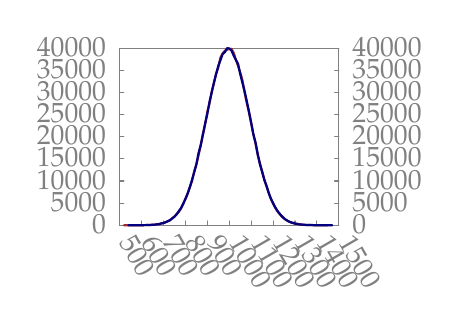
\begin{tikzpicture}[gnuplot, scale=0.3]
%% generated with GNUPLOT 5.2p2 (Lua 5.3; terminal rev. 99, script rev. 102)
%% wo 11 jul 2018 09:51:59 CEST
\path (0.000,0.000) rectangle (12.500,8.750);
\gpcolor{rgb color={0.502,0.502,0.502}}
\gpsetlinetype{gp lt border}
\gpsetdashtype{gp dt solid}
\gpsetlinewidth{1.00}
\draw[gp path] (1.380,0.945)--(1.560,0.945);
\node[gp node right] at (1.196,0.945) {$0$};
\draw[gp path] (1.380,1.882)--(1.560,1.882);
\node[gp node right] at (1.196,1.882) {$5000$};
\draw[gp path] (1.380,2.819)--(1.560,2.819);
\node[gp node right] at (1.196,2.819) {$10000$};
\draw[gp path] (1.380,3.756)--(1.560,3.756);
\node[gp node right] at (1.196,3.756) {$15000$};
\draw[gp path] (1.380,4.693)--(1.560,4.693);
\node[gp node right] at (1.196,4.693) {$20000$};
\draw[gp path] (1.380,5.630)--(1.560,5.630);
\node[gp node right] at (1.196,5.630) {$25000$};
\draw[gp path] (1.380,6.567)--(1.560,6.567);
\node[gp node right] at (1.196,6.567) {$30000$};
\draw[gp path] (1.380,7.504)--(1.560,7.504);
\node[gp node right] at (1.196,7.504) {$35000$};
\draw[gp path] (1.380,8.441)--(1.560,8.441);
\node[gp node right] at (1.196,8.441) {$40000$};
\draw[gp path] (1.380,0.945)--(1.380,1.125);
\node[gp node left,rotate=-60] at (1.380,0.761) {$500$};
\draw[gp path] (2.308,0.945)--(2.308,1.125);
\node[gp node left,rotate=-60] at (2.308,0.761) {$600$};
\draw[gp path] (3.236,0.945)--(3.236,1.125);
\node[gp node left,rotate=-60] at (3.236,0.761) {$700$};
\draw[gp path] (4.164,0.945)--(4.164,1.125);
\node[gp node left,rotate=-60] at (4.164,0.761) {$800$};
\draw[gp path] (5.092,0.945)--(5.092,1.125);
\node[gp node left,rotate=-60] at (5.092,0.761) {$900$};
\draw[gp path] (6.020,0.945)--(6.020,1.125);
\node[gp node left,rotate=-60] at (6.020,0.761) {$1000$};
\draw[gp path] (6.947,0.945)--(6.947,1.125);
\node[gp node left,rotate=-60] at (6.947,0.761) {$1100$};
\draw[gp path] (7.875,0.945)--(7.875,1.125);
\node[gp node left,rotate=-60] at (7.875,0.761) {$1200$};
\draw[gp path] (8.803,0.945)--(8.803,1.125);
\node[gp node left,rotate=-60] at (8.803,0.761) {$1300$};
\draw[gp path] (9.731,0.945)--(9.731,1.125);
\node[gp node left,rotate=-60] at (9.731,0.761) {$1400$};
\draw[gp path] (10.659,0.945)--(10.659,1.125);
\node[gp node left,rotate=-60] at (10.659,0.761) {$1500$};
\draw[gp path] (10.659,0.945)--(10.479,0.945);
\node[gp node left] at (10.843,0.945) {$0$};
\draw[gp path] (10.659,1.882)--(10.479,1.882);
\node[gp node left] at (10.843,1.882) {$5000$};
\draw[gp path] (10.659,2.819)--(10.479,2.819);
\node[gp node left] at (10.843,2.819) {$10000$};
\draw[gp path] (10.659,3.756)--(10.479,3.756);
\node[gp node left] at (10.843,3.756) {$15000$};
\draw[gp path] (10.659,4.693)--(10.479,4.693);
\node[gp node left] at (10.843,4.693) {$20000$};
\draw[gp path] (10.659,5.630)--(10.479,5.630);
\node[gp node left] at (10.843,5.630) {$25000$};
\draw[gp path] (10.659,6.567)--(10.479,6.567);
\node[gp node left] at (10.843,6.567) {$30000$};
\draw[gp path] (10.659,7.504)--(10.479,7.504);
\node[gp node left] at (10.843,7.504) {$35000$};
\draw[gp path] (10.659,8.441)--(10.479,8.441);
\node[gp node left] at (10.843,8.441) {$40000$};
\draw[gp path] (1.380,8.441)--(1.380,0.945)--(10.659,0.945)--(10.659,8.441)--cycle;
\gpcolor{rgb color={0.647,0.165,0.165}}
\gpsetlinewidth{2.00}
\draw[gp path] (1.566,0.945)--(1.658,0.945)--(1.751,0.945)--(1.844,0.946)--(1.937,0.946)%
  --(2.030,0.946)--(2.122,0.946)--(2.215,0.946)--(2.308,0.947)--(2.401,0.949)--(2.493,0.951)%
  --(2.586,0.956)--(2.679,0.958)--(2.772,0.965)--(2.865,0.971)--(2.957,0.979)--(3.050,0.995)%
  --(3.143,1.022)--(3.236,1.043)--(3.329,1.074)--(3.421,1.119)--(3.514,1.158)--(3.607,1.245)%
  --(3.700,1.318)--(3.793,1.418)--(3.885,1.510)--(3.978,1.654)--(4.071,1.847)--(4.164,2.068)%
  --(4.256,2.284)--(4.349,2.546)--(4.442,2.813)--(4.535,3.217)--(4.628,3.513)--(4.720,3.909)%
  --(4.813,4.328)--(4.906,4.805)--(4.999,5.224)--(5.092,5.742)--(5.184,6.100)--(5.277,6.609)%
  --(5.370,6.944)--(5.463,7.364)--(5.556,7.626)--(5.648,8.046)--(5.741,8.217)--(5.834,8.335)%
  --(5.927,8.377)--(6.020,8.408)--(6.112,8.412)--(6.205,8.247)--(6.298,7.959)--(6.391,7.697)%
  --(6.483,7.412)--(6.576,7.088)--(6.669,6.575)--(6.762,6.121)--(6.855,5.720)--(6.947,5.295)%
  --(7.040,4.797)--(7.133,4.406)--(7.226,3.920)--(7.319,3.557)--(7.411,3.237)--(7.504,2.887)%
  --(7.597,2.595)--(7.690,2.320)--(7.783,2.063)--(7.875,1.859)--(7.968,1.681)--(8.061,1.535)%
  --(8.154,1.416)--(8.246,1.306)--(8.339,1.233)--(8.432,1.164)--(8.525,1.114)--(8.618,1.070)%
  --(8.710,1.046)--(8.803,1.020)--(8.896,1.001)--(8.989,0.987)--(9.082,0.972)--(9.174,0.962)%
  --(9.267,0.958)--(9.360,0.955)--(9.453,0.951)--(9.546,0.949)--(9.638,0.948)--(9.731,0.947)%
  --(9.824,0.947)--(9.917,0.946)--(10.009,0.946)--(10.102,0.945)--(10.195,0.945);
\gpcolor{rgb color={0.000,0.000,0.502}}
\draw[gp path] (1.751,0.945)--(1.937,0.946)--(2.030,0.946)--(2.122,0.946)--(2.215,0.947)%
  --(2.308,0.949)--(2.401,0.949)--(2.493,0.950)--(2.586,0.954)--(2.679,0.958)--(2.772,0.965)%
  --(2.865,0.971)--(2.957,0.982)--(3.050,0.990)--(3.143,1.022)--(3.236,1.036)--(3.329,1.076)%
  --(3.421,1.116)--(3.514,1.160)--(3.607,1.233)--(3.700,1.304)--(3.793,1.406)--(3.885,1.544)%
  --(3.978,1.673)--(4.071,1.860)--(4.164,2.052)--(4.256,2.279)--(4.349,2.552)--(4.442,2.862)%
  --(4.535,3.184)--(4.628,3.532)--(4.720,4.001)--(4.813,4.339)--(4.906,4.790)--(4.999,5.249)%
  --(5.092,5.663)--(5.184,6.166)--(5.277,6.562)--(5.370,6.985)--(5.463,7.339)--(5.556,7.690)%
  --(5.648,7.939)--(5.741,8.192)--(5.834,8.274)--(5.927,8.437)--(6.020,8.430)--(6.112,8.344)%
  --(6.205,8.134)--(6.298,7.948)--(6.391,7.778)--(6.483,7.355)--(6.576,6.979)--(6.669,6.618)%
  --(6.762,6.195)--(6.855,5.757)--(6.947,5.272)--(7.040,4.798)--(7.133,4.439)--(7.226,3.952)%
  --(7.319,3.525)--(7.411,3.202)--(7.504,2.859)--(7.597,2.612)--(7.690,2.307)--(7.783,2.068)%
  --(7.875,1.886)--(7.968,1.703)--(8.061,1.551)--(8.154,1.434)--(8.246,1.331)--(8.339,1.236)%
  --(8.432,1.167)--(8.525,1.111)--(8.618,1.072)--(8.710,1.040)--(8.803,1.015)--(8.896,1.000)%
  --(8.989,0.979)--(9.082,0.975)--(9.174,0.967)--(9.267,0.958)--(9.360,0.954)--(9.453,0.953)%
  --(9.546,0.951)--(9.638,0.947)--(9.731,0.948)--(9.824,0.946)--(9.917,0.947)--(10.009,0.946)%
  --(10.381,0.946);
%% coordinates of the plot area
\gpdefrectangularnode{gp plot 1}{\pgfpoint{1.380cm}{0.945cm}}{\pgfpoint{10.659cm}{8.441cm}}
\end{tikzpicture}
%% gnuplot variables

\end{tabular}
\end{center}
\caption{\label{fig:inputselection:normal_1to1_randomOff}
  Random-until-value-reached, for a 1:1 ratio of deposits
  and withdrawals, both drawn from a normal distribution with mean 1000.
}
\end{figure}

This brings us to the topic of active UTxO management. In an ideal case, coin
selection algorithms should, over time, create a UTxO that has ``useful'' outputs;
that is, outputs that allow us to process future payments with a minimum number
of inputs. We can take advantage of self organisation again:
%
\begin{quote}
\textbf{Self organisation principle 2}. If for each payment request for value
$x$ we create a change output roughly of the same value $x$, then we will end up
with a lot of change outputs in our UTxO of size $x$ \emph{precisely when} we
have a lot of payment requests of size $x$.
\end{quote}
%
We will consider some details of how to achieve this in the next section. For
now, Figure~\ref{fig:inputselection:normal_1to1_randomOn} shows what the effect
of this is on the UTxO. The graph in the bottom right, which we've ignored so
far, records the change:payment ratio. A value near zero means a very small
change output (i.e., dust); a very high value would be the result of using a
huge UTxO entry for a much smaller payment. A value around 1 is perfect, and
means that we are generating change outputs of equal value as the payments.

\begin{figure}[p]
\begin{center}
\scriptsize
\begin{tabular}{ll}
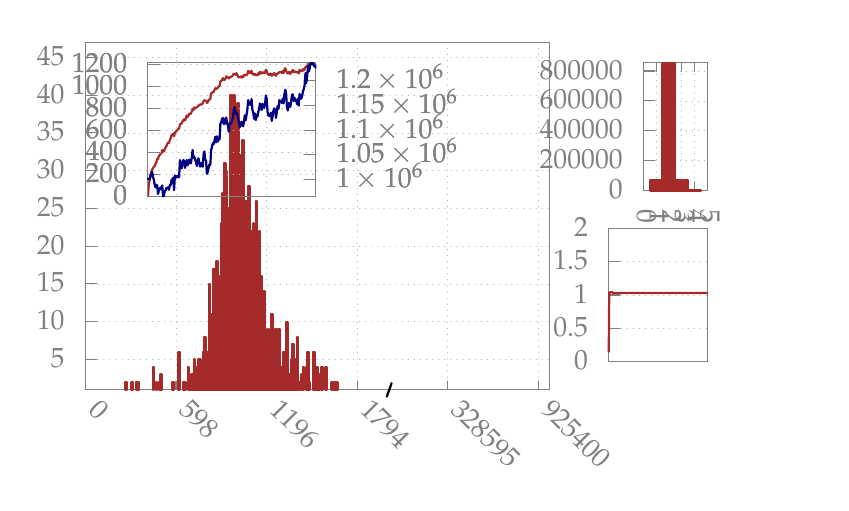
\begin{tikzpicture}[gnuplot, xscale=0.8, yscale=0.6]
%% generated with GNUPLOT 5.2p2 (Lua 5.3; terminal rev. 99, script rev. 102)
%% wo 11 jul 2018 10:38:03 CEST
\path (0.000,0.000) rectangle (12.500,8.750);
\gpcolor{color=gp lt color axes}
\gpsetlinetype{gp lt axes}
\gpsetdashtype{gp dt axes}
\gpsetlinewidth{0.50}
\draw[gp path] (0.828,1.727)--(8.197,1.727);
\gpcolor{rgb color={0.502,0.502,0.502}}
\gpsetlinetype{gp lt border}
\gpsetdashtype{gp dt solid}
\gpsetlinewidth{1.00}
\draw[gp path] (0.828,1.727)--(1.008,1.727);
\node[gp node right] at (0.644,1.727) {$5$};
\gpcolor{color=gp lt color axes}
\gpsetlinetype{gp lt axes}
\gpsetdashtype{gp dt axes}
\gpsetlinewidth{0.50}
\draw[gp path] (0.828,2.527)--(8.197,2.527);
\gpcolor{rgb color={0.502,0.502,0.502}}
\gpsetlinetype{gp lt border}
\gpsetdashtype{gp dt solid}
\gpsetlinewidth{1.00}
\draw[gp path] (0.828,2.527)--(1.008,2.527);
\node[gp node right] at (0.644,2.527) {$10$};
\gpcolor{color=gp lt color axes}
\gpsetlinetype{gp lt axes}
\gpsetdashtype{gp dt axes}
\gpsetlinewidth{0.50}
\draw[gp path] (0.828,3.326)--(8.197,3.326);
\gpcolor{rgb color={0.502,0.502,0.502}}
\gpsetlinetype{gp lt border}
\gpsetdashtype{gp dt solid}
\gpsetlinewidth{1.00}
\draw[gp path] (0.828,3.326)--(1.008,3.326);
\node[gp node right] at (0.644,3.326) {$15$};
\gpcolor{color=gp lt color axes}
\gpsetlinetype{gp lt axes}
\gpsetdashtype{gp dt axes}
\gpsetlinewidth{0.50}
\draw[gp path] (0.828,4.125)--(8.197,4.125);
\gpcolor{rgb color={0.502,0.502,0.502}}
\gpsetlinetype{gp lt border}
\gpsetdashtype{gp dt solid}
\gpsetlinewidth{1.00}
\draw[gp path] (0.828,4.125)--(1.008,4.125);
\node[gp node right] at (0.644,4.125) {$20$};
\gpcolor{color=gp lt color axes}
\gpsetlinetype{gp lt axes}
\gpsetdashtype{gp dt axes}
\gpsetlinewidth{0.50}
\draw[gp path] (0.828,4.924)--(8.197,4.924);
\gpcolor{rgb color={0.502,0.502,0.502}}
\gpsetlinetype{gp lt border}
\gpsetdashtype{gp dt solid}
\gpsetlinewidth{1.00}
\draw[gp path] (0.828,4.924)--(1.008,4.924);
\node[gp node right] at (0.644,4.924) {$25$};
\gpcolor{color=gp lt color axes}
\gpsetlinetype{gp lt axes}
\gpsetdashtype{gp dt axes}
\gpsetlinewidth{0.50}
\draw[gp path] (0.828,5.724)--(8.197,5.724);
\gpcolor{rgb color={0.502,0.502,0.502}}
\gpsetlinetype{gp lt border}
\gpsetdashtype{gp dt solid}
\gpsetlinewidth{1.00}
\draw[gp path] (0.828,5.724)--(1.008,5.724);
\node[gp node right] at (0.644,5.724) {$30$};
\gpcolor{color=gp lt color axes}
\gpsetlinetype{gp lt axes}
\gpsetdashtype{gp dt axes}
\gpsetlinewidth{0.50}
\draw[gp path] (0.828,6.523)--(8.197,6.523);
\gpcolor{rgb color={0.502,0.502,0.502}}
\gpsetlinetype{gp lt border}
\gpsetdashtype{gp dt solid}
\gpsetlinewidth{1.00}
\draw[gp path] (0.828,6.523)--(1.008,6.523);
\node[gp node right] at (0.644,6.523) {$35$};
\gpcolor{color=gp lt color axes}
\gpsetlinetype{gp lt axes}
\gpsetdashtype{gp dt axes}
\gpsetlinewidth{0.50}
\draw[gp path] (0.828,7.322)--(8.197,7.322);
\gpcolor{rgb color={0.502,0.502,0.502}}
\gpsetlinetype{gp lt border}
\gpsetdashtype{gp dt solid}
\gpsetlinewidth{1.00}
\draw[gp path] (0.828,7.322)--(1.008,7.322);
\node[gp node right] at (0.644,7.322) {$40$};
\gpcolor{color=gp lt color axes}
\gpsetlinetype{gp lt axes}
\gpsetdashtype{gp dt axes}
\gpsetlinewidth{0.50}
\draw[gp path] (0.828,8.121)--(8.197,8.121);
\gpcolor{rgb color={0.502,0.502,0.502}}
\gpsetlinetype{gp lt border}
\gpsetdashtype{gp dt solid}
\gpsetlinewidth{1.00}
\draw[gp path] (0.828,8.121)--(1.008,8.121);
\node[gp node right] at (0.644,8.121) {$45$};
\gpcolor{color=gp lt color axes}
\gpsetlinetype{gp lt axes}
\gpsetdashtype{gp dt axes}
\gpsetlinewidth{0.50}
\draw[gp path] (0.828,1.088)--(0.828,8.441);
\gpcolor{rgb color={0.502,0.502,0.502}}
\gpsetlinetype{gp lt border}
\gpsetdashtype{gp dt solid}
\gpsetlinewidth{1.00}
\draw[gp path] (0.828,1.088)--(0.828,1.268);
\node[gp node left,rotate=-45] at (0.828,0.904) {$0$};
\gpcolor{color=gp lt color axes}
\gpsetlinetype{gp lt axes}
\gpsetdashtype{gp dt axes}
\gpsetlinewidth{0.50}
\draw[gp path] (2.266,1.088)--(2.266,8.441);
\gpcolor{rgb color={0.502,0.502,0.502}}
\gpsetlinetype{gp lt border}
\gpsetdashtype{gp dt solid}
\gpsetlinewidth{1.00}
\draw[gp path] (2.266,1.088)--(2.266,1.268);
\node[gp node left,rotate=-45] at (2.266,0.904) {$598$};
\gpcolor{color=gp lt color axes}
\gpsetlinetype{gp lt axes}
\gpsetdashtype{gp dt axes}
\gpsetlinewidth{0.50}
\draw[gp path] (3.704,1.088)--(3.704,8.441);
\gpcolor{rgb color={0.502,0.502,0.502}}
\gpsetlinetype{gp lt border}
\gpsetdashtype{gp dt solid}
\gpsetlinewidth{1.00}
\draw[gp path] (3.704,1.088)--(3.704,1.268);
\node[gp node left,rotate=-45] at (3.704,0.904) {$1196$};
\gpcolor{color=gp lt color axes}
\gpsetlinetype{gp lt axes}
\gpsetdashtype{gp dt axes}
\gpsetlinewidth{0.50}
\draw[gp path] (5.142,1.088)--(5.142,8.441);
\gpcolor{rgb color={0.502,0.502,0.502}}
\gpsetlinetype{gp lt border}
\gpsetdashtype{gp dt solid}
\gpsetlinewidth{1.00}
\draw[gp path] (5.142,1.088)--(5.142,1.268);
\node[gp node left,rotate=-45] at (5.142,0.904) {$1794$};
\gpcolor{color=gp lt color axes}
\gpsetlinetype{gp lt axes}
\gpsetdashtype{gp dt axes}
\gpsetlinewidth{0.50}
\draw[gp path] (6.579,1.088)--(6.579,8.441);
\gpcolor{rgb color={0.502,0.502,0.502}}
\gpsetlinetype{gp lt border}
\gpsetdashtype{gp dt solid}
\gpsetlinewidth{1.00}
\draw[gp path] (6.579,1.088)--(6.579,1.268);
\node[gp node left,rotate=-45] at (6.579,0.904) {$328595$};
\gpcolor{color=gp lt color axes}
\gpsetlinetype{gp lt axes}
\gpsetdashtype{gp dt axes}
\gpsetlinewidth{0.50}
\draw[gp path] (8.017,1.088)--(8.017,8.441);
\gpcolor{rgb color={0.502,0.502,0.502}}
\gpsetlinetype{gp lt border}
\gpsetdashtype{gp dt solid}
\gpsetlinewidth{1.00}
\draw[gp path] (8.017,1.088)--(8.017,1.268);
\node[gp node left,rotate=-45] at (8.017,0.904) {$925400$};
\draw[gp path] (0.828,8.441)--(0.828,1.088)--(8.197,1.088)--(8.197,8.441)--cycle;
\gpcolor{rgb color={0.647,0.165,0.165}}
\gpsetlinewidth{2.00}
\draw[gp path] (1.465,1.088)--(1.465,1.248)--(1.489,1.248)--(1.489,1.088)--cycle;
\draw[gp path] (1.561,1.088)--(1.561,1.248)--(1.585,1.248)--(1.585,1.088)--cycle;
\draw[gp path] (1.633,1.088)--(1.633,1.248)--(1.658,1.248)--(1.658,1.088)--cycle;
\draw[gp path] (1.658,1.088)--(1.658,1.248)--(1.682,1.248)--(1.682,1.088)--cycle;
\draw[gp path] (1.898,1.088)--(1.898,1.568)--(1.922,1.568)--(1.922,1.088)--cycle;
\draw[gp path] (1.946,1.088)--(1.946,1.248)--(1.970,1.248)--(1.970,1.088)--cycle;
\draw[gp path] (1.994,1.088)--(1.994,1.248)--(2.018,1.248)--(2.018,1.088)--cycle;
\draw[gp path] (2.018,1.088)--(2.018,1.408)--(2.042,1.408)--(2.042,1.088)--cycle;
\draw[gp path] (2.211,1.088)--(2.211,1.248)--(2.235,1.248)--(2.235,1.088)--cycle;
\draw[gp path] (2.307,1.088)--(2.307,1.887)--(2.331,1.887)--(2.331,1.088)--cycle;
\draw[gp path] (2.379,1.088)--(2.379,1.248)--(2.403,1.248)--(2.403,1.088)--cycle;
\draw[gp path] (2.403,1.088)--(2.403,1.248)--(2.427,1.248)--(2.427,1.088)--cycle;
\draw[gp path] (2.451,1.088)--(2.451,1.568)--(2.475,1.568)--(2.475,1.088)--cycle;
\draw[gp path] (2.475,1.088)--(2.475,1.248)--(2.499,1.248)--(2.499,1.088)--cycle;
\draw[gp path] (2.499,1.088)--(2.499,1.408)--(2.523,1.408)--(2.523,1.088)--cycle;
\draw[gp path] (2.523,1.088)--(2.523,1.408)--(2.547,1.408)--(2.547,1.088)--cycle;
\draw[gp path] (2.547,1.088)--(2.547,1.727)--(2.571,1.727)--(2.571,1.088)--cycle;
\draw[gp path] (2.571,1.088)--(2.571,1.568)--(2.595,1.568)--(2.595,1.088)--cycle;
\draw[gp path] (2.595,1.088)--(2.595,1.408)--(2.619,1.408)--(2.619,1.088)--cycle;
\draw[gp path] (2.619,1.088)--(2.619,1.727)--(2.643,1.727)--(2.643,1.088)--cycle;
\draw[gp path] (2.643,1.088)--(2.643,1.727)--(2.667,1.727)--(2.667,1.088)--cycle;
\draw[gp path] (2.667,1.088)--(2.667,1.568)--(2.691,1.568)--(2.691,1.088)--cycle;
\draw[gp path] (2.691,1.088)--(2.691,1.887)--(2.715,1.887)--(2.715,1.088)--cycle;
\draw[gp path] (2.715,1.088)--(2.715,2.207)--(2.740,2.207)--(2.740,1.088)--cycle;
\draw[gp path] (2.740,1.088)--(2.740,1.887)--(2.764,1.887)--(2.764,1.088)--cycle;
\draw[gp path] (2.764,1.088)--(2.764,1.887)--(2.788,1.887)--(2.788,1.088)--cycle;
\draw[gp path] (2.788,1.088)--(2.788,3.326)--(2.812,3.326)--(2.812,1.088)--cycle;
\draw[gp path] (2.812,1.088)--(2.812,2.686)--(2.836,2.686)--(2.836,1.088)--cycle;
\draw[gp path] (2.836,1.088)--(2.836,2.686)--(2.860,2.686)--(2.860,1.088)--cycle;
\draw[gp path] (2.860,1.088)--(2.860,3.646)--(2.884,3.646)--(2.884,1.088)--cycle;
\draw[gp path] (2.884,1.088)--(2.884,3.646)--(2.908,3.646)--(2.908,1.088)--cycle;
\draw[gp path] (2.908,1.088)--(2.908,3.805)--(2.932,3.805)--(2.932,1.088)--cycle;
\draw[gp path] (2.932,1.088)--(2.932,3.486)--(2.956,3.486)--(2.956,1.088)--cycle;
\draw[gp path] (2.956,1.088)--(2.956,2.686)--(2.980,2.686)--(2.980,1.088)--cycle;
\draw[gp path] (2.980,1.088)--(2.980,4.605)--(3.004,4.605)--(3.004,1.088)--cycle;
\draw[gp path] (3.004,1.088)--(3.004,5.244)--(3.028,5.244)--(3.028,1.088)--cycle;
\draw[gp path] (3.028,1.088)--(3.028,5.883)--(3.052,5.883)--(3.052,1.088)--cycle;
\draw[gp path] (3.052,1.088)--(3.052,5.724)--(3.076,5.724)--(3.076,1.088)--cycle;
\draw[gp path] (3.076,1.088)--(3.076,4.924)--(3.100,4.924)--(3.100,1.088)--cycle;
\draw[gp path] (3.100,1.088)--(3.100,4.765)--(3.124,4.765)--(3.124,1.088)--cycle;
\draw[gp path] (3.124,1.088)--(3.124,7.322)--(3.148,7.322)--(3.148,1.088)--cycle;
\draw[gp path] (3.148,1.088)--(3.148,6.363)--(3.172,6.363)--(3.172,1.088)--cycle;
\draw[gp path] (3.172,1.088)--(3.172,7.322)--(3.196,7.322)--(3.196,1.088)--cycle;
\draw[gp path] (3.196,1.088)--(3.196,5.404)--(3.220,5.404)--(3.220,1.088)--cycle;
\draw[gp path] (3.220,1.088)--(3.220,5.724)--(3.244,5.724)--(3.244,1.088)--cycle;
\draw[gp path] (3.244,1.088)--(3.244,7.162)--(3.269,7.162)--(3.269,1.088)--cycle;
\draw[gp path] (3.269,1.088)--(3.269,6.043)--(3.293,6.043)--(3.293,1.088)--cycle;
\draw[gp path] (3.293,1.088)--(3.293,5.404)--(3.317,5.404)--(3.317,1.088)--cycle;
\draw[gp path] (3.317,1.088)--(3.317,6.363)--(3.341,6.363)--(3.341,1.088)--cycle;
\draw[gp path] (3.341,1.088)--(3.341,4.445)--(3.365,4.445)--(3.365,1.088)--cycle;
\draw[gp path] (3.365,1.088)--(3.365,5.084)--(3.389,5.084)--(3.389,1.088)--cycle;
\draw[gp path] (3.389,1.088)--(3.389,4.285)--(3.413,4.285)--(3.413,1.088)--cycle;
\draw[gp path] (3.413,1.088)--(3.413,5.404)--(3.437,5.404)--(3.437,1.088)--cycle;
\draw[gp path] (3.437,1.088)--(3.437,4.285)--(3.461,4.285)--(3.461,1.088)--cycle;
\draw[gp path] (3.461,1.088)--(3.461,4.445)--(3.485,4.445)--(3.485,1.088)--cycle;
\draw[gp path] (3.485,1.088)--(3.485,4.605)--(3.509,4.605)--(3.509,1.088)--cycle;
\draw[gp path] (3.509,1.088)--(3.509,4.445)--(3.533,4.445)--(3.533,1.088)--cycle;
\draw[gp path] (3.533,1.088)--(3.533,5.084)--(3.557,5.084)--(3.557,1.088)--cycle;
\draw[gp path] (3.557,1.088)--(3.557,3.805)--(3.581,3.805)--(3.581,1.088)--cycle;
\draw[gp path] (3.581,1.088)--(3.581,4.445)--(3.605,4.445)--(3.605,1.088)--cycle;
\draw[gp path] (3.605,1.088)--(3.605,3.486)--(3.629,3.486)--(3.629,1.088)--cycle;
\draw[gp path] (3.629,1.088)--(3.629,2.047)--(3.653,2.047)--(3.653,1.088)--cycle;
\draw[gp path] (3.653,1.088)--(3.653,3.166)--(3.677,3.166)--(3.677,1.088)--cycle;
\draw[gp path] (3.677,1.088)--(3.677,2.367)--(3.701,2.367)--(3.701,1.088)--cycle;
\draw[gp path] (3.701,1.088)--(3.701,2.047)--(3.725,2.047)--(3.725,1.088)--cycle;
\draw[gp path] (3.725,1.088)--(3.725,2.367)--(3.749,2.367)--(3.749,1.088)--cycle;
\draw[gp path] (3.749,1.088)--(3.749,1.887)--(3.773,1.887)--(3.773,1.088)--cycle;
\draw[gp path] (3.773,1.088)--(3.773,2.686)--(3.797,2.686)--(3.797,1.088)--cycle;
\draw[gp path] (3.797,1.088)--(3.797,2.367)--(3.822,2.367)--(3.822,1.088)--cycle;
\draw[gp path] (3.822,1.088)--(3.822,1.887)--(3.846,1.887)--(3.846,1.088)--cycle;
\draw[gp path] (3.846,1.088)--(3.846,2.367)--(3.870,2.367)--(3.870,1.088)--cycle;
\draw[gp path] (3.870,1.088)--(3.870,2.047)--(3.894,2.047)--(3.894,1.088)--cycle;
\draw[gp path] (3.894,1.088)--(3.894,2.367)--(3.918,2.367)--(3.918,1.088)--cycle;
\draw[gp path] (3.918,1.088)--(3.918,1.408)--(3.942,1.408)--(3.942,1.088)--cycle;
\draw[gp path] (3.942,1.088)--(3.942,1.568)--(3.966,1.568)--(3.966,1.088)--cycle;
\draw[gp path] (3.966,1.088)--(3.966,1.887)--(3.990,1.887)--(3.990,1.088)--cycle;
\draw[gp path] (3.990,1.088)--(3.990,1.727)--(4.014,1.727)--(4.014,1.088)--cycle;
\draw[gp path] (4.014,1.088)--(4.014,2.527)--(4.038,2.527)--(4.038,1.088)--cycle;
\draw[gp path] (4.038,1.088)--(4.038,1.408)--(4.062,1.408)--(4.062,1.088)--cycle;
\draw[gp path] (4.062,1.088)--(4.062,1.408)--(4.086,1.408)--(4.086,1.088)--cycle;
\draw[gp path] (4.086,1.088)--(4.086,1.727)--(4.110,1.727)--(4.110,1.088)--cycle;
\draw[gp path] (4.110,1.088)--(4.110,2.047)--(4.134,2.047)--(4.134,1.088)--cycle;
\draw[gp path] (4.134,1.088)--(4.134,1.727)--(4.158,1.727)--(4.158,1.088)--cycle;
\draw[gp path] (4.158,1.088)--(4.158,1.727)--(4.182,1.727)--(4.182,1.088)--cycle;
\draw[gp path] (4.182,1.088)--(4.182,2.207)--(4.206,2.207)--(4.206,1.088)--cycle;
\draw[gp path] (4.206,1.088)--(4.206,1.248)--(4.230,1.248)--(4.230,1.088)--cycle;
\draw[gp path] (4.254,1.088)--(4.254,1.408)--(4.278,1.408)--(4.278,1.088)--cycle;
\draw[gp path] (4.278,1.088)--(4.278,1.568)--(4.302,1.568)--(4.302,1.088)--cycle;
\draw[gp path] (4.326,1.088)--(4.326,1.568)--(4.351,1.568)--(4.351,1.088)--cycle;
\draw[gp path] (4.351,1.088)--(4.351,1.887)--(4.375,1.887)--(4.375,1.088)--cycle;
\draw[gp path] (4.375,1.088)--(4.375,1.248)--(4.399,1.248)--(4.399,1.088)--cycle;
\draw[gp path] (4.447,1.088)--(4.447,1.887)--(4.471,1.887)--(4.471,1.088)--cycle;
\draw[gp path] (4.471,1.088)--(4.471,1.248)--(4.495,1.248)--(4.495,1.088)--cycle;
\draw[gp path] (4.495,1.088)--(4.495,1.568)--(4.519,1.568)--(4.519,1.088)--cycle;
\draw[gp path] (4.519,1.088)--(4.519,1.408)--(4.543,1.408)--(4.543,1.088)--cycle;
\draw[gp path] (4.567,1.088)--(4.567,1.568)--(4.591,1.568)--(4.591,1.088)--cycle;
\draw[gp path] (4.639,1.088)--(4.639,1.568)--(4.663,1.568)--(4.663,1.088)--cycle;
\draw[gp path] (4.735,1.088)--(4.735,1.248)--(4.759,1.248)--(4.759,1.088)--cycle;
\draw[gp path] (4.783,1.088)--(4.783,1.248)--(4.807,1.248)--(4.807,1.088)--cycle;
\draw[gp path] (4.807,1.088)--(4.807,1.248)--(4.831,1.248)--(4.831,1.088)--cycle;
\gpcolor{color=gp lt color border}
\draw[gp path](5.613,0.941)--(5.689,1.225);
%% coordinates of the plot area
\gpdefrectangularnode{gp plot 1}{\pgfpoint{0.828cm}{1.088cm}}{\pgfpoint{8.197cm}{8.441cm}}
\gpcolor{color=gp lt color axes}
\gpsetlinetype{gp lt axes}
\gpsetdashtype{gp dt axes}
\gpsetlinewidth{0.50}
\draw[gp path] (1.821,5.175)--(4.482,5.175);
\gpcolor{rgb color={0.502,0.502,0.502}}
\gpsetlinetype{gp lt border}
\gpsetdashtype{gp dt solid}
\gpsetlinewidth{1.00}
\draw[gp path] (1.821,5.175)--(2.001,5.175);
\node[gp node right] at (1.637,5.175) {$0$};
\gpcolor{color=gp lt color axes}
\gpsetlinetype{gp lt axes}
\gpsetdashtype{gp dt axes}
\gpsetlinewidth{0.50}
\draw[gp path] (1.821,5.642)--(4.482,5.642);
\gpcolor{rgb color={0.502,0.502,0.502}}
\gpsetlinetype{gp lt border}
\gpsetdashtype{gp dt solid}
\gpsetlinewidth{1.00}
\draw[gp path] (1.821,5.642)--(2.001,5.642);
\node[gp node right] at (1.637,5.642) {$200$};
\gpcolor{color=gp lt color axes}
\gpsetlinetype{gp lt axes}
\gpsetdashtype{gp dt axes}
\gpsetlinewidth{0.50}
\draw[gp path] (1.821,6.109)--(4.482,6.109);
\gpcolor{rgb color={0.502,0.502,0.502}}
\gpsetlinetype{gp lt border}
\gpsetdashtype{gp dt solid}
\gpsetlinewidth{1.00}
\draw[gp path] (1.821,6.109)--(2.001,6.109);
\node[gp node right] at (1.637,6.109) {$400$};
\gpcolor{color=gp lt color axes}
\gpsetlinetype{gp lt axes}
\gpsetdashtype{gp dt axes}
\gpsetlinewidth{0.50}
\draw[gp path] (1.821,6.576)--(4.482,6.576);
\gpcolor{rgb color={0.502,0.502,0.502}}
\gpsetlinetype{gp lt border}
\gpsetdashtype{gp dt solid}
\gpsetlinewidth{1.00}
\draw[gp path] (1.821,6.576)--(2.001,6.576);
\node[gp node right] at (1.637,6.576) {$600$};
\gpcolor{color=gp lt color axes}
\gpsetlinetype{gp lt axes}
\gpsetdashtype{gp dt axes}
\gpsetlinewidth{0.50}
\draw[gp path] (1.821,7.042)--(4.482,7.042);
\gpcolor{rgb color={0.502,0.502,0.502}}
\gpsetlinetype{gp lt border}
\gpsetdashtype{gp dt solid}
\gpsetlinewidth{1.00}
\draw[gp path] (1.821,7.042)--(2.001,7.042);
\node[gp node right] at (1.637,7.042) {$800$};
\gpcolor{color=gp lt color axes}
\gpsetlinetype{gp lt axes}
\gpsetdashtype{gp dt axes}
\gpsetlinewidth{0.50}
\draw[gp path] (1.821,7.509)--(4.482,7.509);
\gpcolor{rgb color={0.502,0.502,0.502}}
\gpsetlinetype{gp lt border}
\gpsetdashtype{gp dt solid}
\gpsetlinewidth{1.00}
\draw[gp path] (1.821,7.509)--(2.001,7.509);
\node[gp node right] at (1.637,7.509) {$1000$};
\gpcolor{color=gp lt color axes}
\gpsetlinetype{gp lt axes}
\gpsetdashtype{gp dt axes}
\gpsetlinewidth{0.50}
\draw[gp path] (1.821,7.976)--(4.482,7.976);
\gpcolor{rgb color={0.502,0.502,0.502}}
\gpsetlinetype{gp lt border}
\gpsetdashtype{gp dt solid}
\gpsetlinewidth{1.00}
\draw[gp path] (1.821,7.976)--(2.001,7.976);
\node[gp node right] at (1.637,7.976) {$1200$};
\draw[gp path] (4.482,5.538)--(4.302,5.538);
\node[gp node left] at (4.666,5.538) {$1\times10^{6}$};
\draw[gp path] (4.482,6.059)--(4.302,6.059);
\node[gp node left] at (4.666,6.059) {$1.05\times10^{6}$};
\draw[gp path] (4.482,6.580)--(4.302,6.580);
\node[gp node left] at (4.666,6.580) {$1.1\times10^{6}$};
\draw[gp path] (4.482,7.102)--(4.302,7.102);
\node[gp node left] at (4.666,7.102) {$1.15\times10^{6}$};
\draw[gp path] (4.482,7.623)--(4.302,7.623);
\node[gp node left] at (4.666,7.623) {$1.2\times10^{6}$};
\draw[gp path] (1.821,8.004)--(1.821,5.180)--(4.482,5.180)--(4.482,8.004)--cycle;
\gpcolor{rgb color={0.647,0.165,0.165}}
\gpsetlinewidth{2.00}
\draw[gp path] (1.821,5.180)--(1.834,5.430)--(1.848,5.518)--(1.861,5.605)--(1.874,5.696)%
  --(1.888,5.747)--(1.901,5.775)--(1.915,5.808)--(1.928,5.819)--(1.941,5.866)--(1.955,5.897)%
  --(1.968,5.974)--(1.981,5.969)--(1.995,6.039)--(2.008,6.051)--(2.022,6.088)--(2.035,6.086)%
  --(2.048,6.160)--(2.062,6.128)--(2.075,6.130)--(2.088,6.179)--(2.102,6.216)--(2.115,6.244)%
  --(2.129,6.293)--(2.142,6.319)--(2.155,6.312)--(2.169,6.370)--(2.182,6.415)--(2.195,6.475)%
  --(2.209,6.475)--(2.222,6.506)--(2.236,6.452)--(2.249,6.527)--(2.262,6.548)--(2.276,6.562)%
  --(2.289,6.585)--(2.302,6.604)--(2.316,6.615)--(2.329,6.697)--(2.343,6.718)--(2.356,6.720)%
  --(2.369,6.767)--(2.383,6.786)--(2.396,6.814)--(2.409,6.786)--(2.423,6.832)--(2.436,6.893)%
  --(2.449,6.860)--(2.463,6.886)--(2.476,6.930)--(2.490,6.919)--(2.503,6.933)--(2.516,6.975)%
  --(2.530,7.031)--(2.543,7.007)--(2.556,7.063)--(2.570,7.035)--(2.583,7.061)--(2.597,7.059)%
  --(2.610,7.080)--(2.623,7.103)--(2.637,7.105)--(2.650,7.129)--(2.663,7.117)--(2.677,7.133)%
  --(2.690,7.147)--(2.704,7.196)--(2.717,7.217)--(2.730,7.203)--(2.744,7.206)--(2.757,7.159)%
  --(2.770,7.171)--(2.784,7.217)--(2.797,7.231)--(2.811,7.234)--(2.824,7.367)--(2.837,7.365)%
  --(2.851,7.390)--(2.864,7.388)--(2.877,7.432)--(2.891,7.467)--(2.904,7.451)--(2.917,7.467)%
  --(2.931,7.481)--(2.944,7.505)--(2.958,7.516)--(2.971,7.610)--(2.984,7.624)--(2.998,7.640)%
  --(3.011,7.684)--(3.024,7.645)--(3.038,7.645)--(3.051,7.668)--(3.065,7.719)--(3.078,7.710)%
  --(3.091,7.701)--(3.105,7.675)--(3.118,7.696)--(3.131,7.705)--(3.145,7.715)--(3.158,7.719)%
  --(3.172,7.754)--(3.185,7.773)--(3.198,7.771)--(3.212,7.754)--(3.225,7.787)--(3.238,7.757)%
  --(3.252,7.710)--(3.265,7.701)--(3.279,7.698)--(3.292,7.705)--(3.305,7.722)--(3.319,7.694)%
  --(3.332,7.708)--(3.345,7.750)--(3.359,7.747)--(3.372,7.736)--(3.386,7.761)--(3.399,7.757)%
  --(3.412,7.836)--(3.426,7.820)--(3.439,7.792)--(3.452,7.794)--(3.466,7.838)--(3.479,7.768)%
  --(3.492,7.773)--(3.506,7.752)--(3.519,7.773)--(3.533,7.743)--(3.546,7.747)--(3.559,7.743)%
  --(3.573,7.787)--(3.586,7.757)--(3.599,7.815)--(3.613,7.801)--(3.626,7.780)--(3.640,7.806)%
  --(3.653,7.801)--(3.666,7.785)--(3.680,7.796)--(3.693,7.859)--(3.706,7.834)--(3.720,7.771)%
  --(3.733,7.764)--(3.747,7.745)--(3.760,7.775)--(3.773,7.780)--(3.787,7.731)--(3.800,7.750)%
  --(3.813,7.768)--(3.827,7.789)--(3.840,7.745)--(3.854,7.733)--(3.867,7.775)--(3.880,7.780)%
  --(3.894,7.792)--(3.907,7.808)--(3.920,7.808)--(3.934,7.817)--(3.947,7.789)--(3.960,7.829)%
  --(3.974,7.789)--(3.987,7.862)--(4.001,7.892)--(4.014,7.838)--(4.027,7.801)--(4.041,7.780)%
  --(4.054,7.799)--(4.067,7.815)--(4.081,7.771)--(4.094,7.806)--(4.108,7.827)--(4.121,7.855)%
  --(4.134,7.806)--(4.148,7.820)--(4.161,7.822)--(4.174,7.801)--(4.188,7.813)--(4.201,7.806)%
  --(4.215,7.785)--(4.228,7.859)--(4.241,7.829)--(4.255,7.836)--(4.268,7.831)--(4.281,7.876)%
  --(4.295,7.843)--(4.308,7.871)--(4.322,7.915)--(4.335,7.918)--(4.348,7.950)--(4.362,7.981)%
  --(4.375,7.934)--(4.388,7.946)--(4.402,7.976)--(4.415,8.004)--(4.429,7.997)--(4.442,7.976)%
  --(4.455,7.969)--(4.469,7.988)--(4.482,7.948);
%% coordinates of the plot area
\gpdefrectangularnode{gp plot 2}{\pgfpoint{1.821cm}{5.180cm}}{\pgfpoint{4.482cm}{8.004cm}}
\gpcolor{color=gp lt color axes}
\gpsetlinetype{gp lt axes}
\gpsetdashtype{gp dt axes}
\gpsetlinewidth{0.50}
\draw[gp path] (1.821,5.175)--(4.482,5.175);
\gpcolor{rgb color={0.502,0.502,0.502}}
\gpsetlinetype{gp lt border}
\gpsetdashtype{gp dt solid}
\gpsetlinewidth{1.00}
\draw[gp path] (1.821,5.175)--(2.001,5.175);
\node[gp node right] at (1.637,5.175) {$0$};
\gpcolor{color=gp lt color axes}
\gpsetlinetype{gp lt axes}
\gpsetdashtype{gp dt axes}
\gpsetlinewidth{0.50}
\draw[gp path] (1.821,5.642)--(4.482,5.642);
\gpcolor{rgb color={0.502,0.502,0.502}}
\gpsetlinetype{gp lt border}
\gpsetdashtype{gp dt solid}
\gpsetlinewidth{1.00}
\draw[gp path] (1.821,5.642)--(2.001,5.642);
\node[gp node right] at (1.637,5.642) {$200$};
\gpcolor{color=gp lt color axes}
\gpsetlinetype{gp lt axes}
\gpsetdashtype{gp dt axes}
\gpsetlinewidth{0.50}
\draw[gp path] (1.821,6.109)--(4.482,6.109);
\gpcolor{rgb color={0.502,0.502,0.502}}
\gpsetlinetype{gp lt border}
\gpsetdashtype{gp dt solid}
\gpsetlinewidth{1.00}
\draw[gp path] (1.821,6.109)--(2.001,6.109);
\node[gp node right] at (1.637,6.109) {$400$};
\gpcolor{color=gp lt color axes}
\gpsetlinetype{gp lt axes}
\gpsetdashtype{gp dt axes}
\gpsetlinewidth{0.50}
\draw[gp path] (1.821,6.576)--(4.482,6.576);
\gpcolor{rgb color={0.502,0.502,0.502}}
\gpsetlinetype{gp lt border}
\gpsetdashtype{gp dt solid}
\gpsetlinewidth{1.00}
\draw[gp path] (1.821,6.576)--(2.001,6.576);
\node[gp node right] at (1.637,6.576) {$600$};
\gpcolor{color=gp lt color axes}
\gpsetlinetype{gp lt axes}
\gpsetdashtype{gp dt axes}
\gpsetlinewidth{0.50}
\draw[gp path] (1.821,7.042)--(4.482,7.042);
\gpcolor{rgb color={0.502,0.502,0.502}}
\gpsetlinetype{gp lt border}
\gpsetdashtype{gp dt solid}
\gpsetlinewidth{1.00}
\draw[gp path] (1.821,7.042)--(2.001,7.042);
\node[gp node right] at (1.637,7.042) {$800$};
\gpcolor{color=gp lt color axes}
\gpsetlinetype{gp lt axes}
\gpsetdashtype{gp dt axes}
\gpsetlinewidth{0.50}
\draw[gp path] (1.821,7.509)--(4.482,7.509);
\gpcolor{rgb color={0.502,0.502,0.502}}
\gpsetlinetype{gp lt border}
\gpsetdashtype{gp dt solid}
\gpsetlinewidth{1.00}
\draw[gp path] (1.821,7.509)--(2.001,7.509);
\node[gp node right] at (1.637,7.509) {$1000$};
\gpcolor{color=gp lt color axes}
\gpsetlinetype{gp lt axes}
\gpsetdashtype{gp dt axes}
\gpsetlinewidth{0.50}
\draw[gp path] (1.821,7.976)--(4.482,7.976);
\gpcolor{rgb color={0.502,0.502,0.502}}
\gpsetlinetype{gp lt border}
\gpsetdashtype{gp dt solid}
\gpsetlinewidth{1.00}
\draw[gp path] (1.821,7.976)--(2.001,7.976);
\node[gp node right] at (1.637,7.976) {$1200$};
\draw[gp path] (4.482,5.538)--(4.302,5.538);
\node[gp node left] at (4.666,5.538) {$1\times10^{6}$};
\draw[gp path] (4.482,6.059)--(4.302,6.059);
\node[gp node left] at (4.666,6.059) {$1.05\times10^{6}$};
\draw[gp path] (4.482,6.580)--(4.302,6.580);
\node[gp node left] at (4.666,6.580) {$1.1\times10^{6}$};
\draw[gp path] (4.482,7.102)--(4.302,7.102);
\node[gp node left] at (4.666,7.102) {$1.15\times10^{6}$};
\draw[gp path] (4.482,7.623)--(4.302,7.623);
\node[gp node left] at (4.666,7.623) {$1.2\times10^{6}$};
\draw[gp path] (1.821,8.004)--(1.821,5.180)--(4.482,5.180)--(4.482,8.004)--cycle;
\gpcolor{rgb color={0.000,0.000,0.502}}
\gpsetlinewidth{2.00}
\draw[gp path] (1.821,5.539)--(1.834,5.557)--(1.848,5.545)--(1.861,5.618)--(1.874,5.637)%
  --(1.888,5.698)--(1.901,5.589)--(1.915,5.534)--(1.928,5.428)--(1.941,5.370)--(1.955,5.420)%
  --(1.968,5.411)--(1.981,5.230)--(1.995,5.307)--(2.008,5.342)--(2.022,5.368)--(2.035,5.326)%
  --(2.048,5.411)--(2.062,5.180)--(2.075,5.198)--(2.088,5.286)--(2.102,5.311)--(2.115,5.359)%
  --(2.129,5.359)--(2.142,5.371)--(2.155,5.320)--(2.169,5.421)--(2.182,5.417)--(2.195,5.530)%
  --(2.209,5.539)--(2.222,5.575)--(2.236,5.310)--(2.249,5.621)--(2.262,5.569)--(2.276,5.602)%
  --(2.289,5.616)--(2.302,5.585)--(2.316,5.586)--(2.329,5.945)--(2.343,5.883)--(2.356,5.770)%
  --(2.369,5.880)--(2.383,5.947)--(2.396,5.928)--(2.409,5.783)--(2.423,5.844)--(2.436,5.950)%
  --(2.449,5.836)--(2.463,5.892)--(2.476,5.958)--(2.490,5.879)--(2.503,5.880)--(2.516,5.989)%
  --(2.530,6.160)--(2.543,5.998)--(2.556,6.020)--(2.570,5.958)--(2.583,5.918)--(2.597,5.821)%
  --(2.610,5.942)--(2.623,5.985)--(2.637,5.883)--(2.650,5.808)--(2.663,5.874)--(2.677,5.888)%
  --(2.690,5.806)--(2.704,6.059)--(2.717,6.130)--(2.730,5.960)--(2.744,5.931)--(2.757,5.655)%
  --(2.770,5.698)--(2.784,5.785)--(2.797,5.860)--(2.811,5.841)--(2.824,6.153)--(2.837,6.226)%
  --(2.851,6.309)--(2.864,6.282)--(2.877,6.350)--(2.891,6.442)--(2.904,6.323)--(2.917,6.450)%
  --(2.931,6.340)--(2.944,6.412)--(2.958,6.382)--(2.971,6.717)--(2.984,6.742)--(2.998,6.824)%
  --(3.011,6.838)--(3.024,6.709)--(3.038,6.711)--(3.051,6.818)--(3.065,6.847)--(3.078,6.724)%
  --(3.091,6.679)--(3.105,6.549)--(3.118,6.730)--(3.131,6.711)--(3.145,6.736)--(3.158,6.801)%
  --(3.172,6.843)--(3.185,7.014)--(3.198,7.072)--(3.212,6.930)--(3.225,6.959)--(3.238,6.927)%
  --(3.252,6.809)--(3.265,6.752)--(3.279,6.644)--(3.292,6.686)--(3.305,6.761)--(3.319,6.691)%
  --(3.332,6.663)--(3.345,6.757)--(3.359,6.895)--(3.372,6.787)--(3.386,6.900)--(3.399,7.013)%
  --(3.412,7.218)--(3.426,7.127)--(3.439,7.159)--(3.452,7.110)--(3.466,7.239)--(3.479,7.010)%
  --(3.492,6.964)--(3.506,6.822)--(3.519,6.936)--(3.533,6.794)--(3.546,6.898)--(3.559,6.867)%
  --(3.573,6.973)--(3.586,7.024)--(3.599,7.147)--(3.613,7.052)--(3.626,7.009)--(3.640,7.136)%
  --(3.653,7.102)--(3.666,7.049)--(3.680,7.132)--(3.693,7.314)--(3.706,7.249)--(3.720,6.968)%
  --(3.733,6.893)--(3.747,6.884)--(3.760,6.887)--(3.773,6.952)--(3.787,6.777)--(3.800,6.880)%
  --(3.813,6.997)--(3.827,7.041)--(3.840,7.009)--(3.854,6.837)--(3.867,6.978)--(3.880,7.092)%
  --(3.894,7.032)--(3.907,7.216)--(3.920,7.196)--(3.934,7.189)--(3.947,7.154)--(3.960,7.250)%
  --(3.974,7.150)--(3.987,7.335)--(4.001,7.435)--(4.014,7.366)--(4.027,7.077)--(4.041,6.996)%
  --(4.054,7.156)--(4.067,7.079)--(4.081,7.076)--(4.094,7.190)--(4.108,7.332)--(4.121,7.336)%
  --(4.134,7.195)--(4.148,7.267)--(4.161,7.204)--(4.174,7.214)--(4.188,7.130)--(4.201,7.245)%
  --(4.215,7.100)--(4.228,7.347)--(4.241,7.241)--(4.255,7.252)--(4.268,7.300)--(4.281,7.395)%
  --(4.295,7.454)--(4.308,7.530)--(4.322,7.789)--(4.335,7.580)--(4.348,7.717)--(4.362,7.938)%
  --(4.375,7.823)--(4.388,7.880)--(4.402,8.004)--(4.415,7.976)--(4.429,7.996)--(4.442,7.999)%
  --(4.455,7.944)--(4.469,7.951)--(4.482,7.903);
\gpcolor{color=gp lt color axes}
\gpsetlinetype{gp lt axes}
\gpsetdashtype{gp dt axes}
\gpsetlinewidth{0.50}
\draw[gp path] (9.688,5.304)--(10.697,5.304);
\gpcolor{rgb color={0.502,0.502,0.502}}
\gpsetlinetype{gp lt border}
\gpsetdashtype{gp dt solid}
\gpsetlinewidth{1.00}
\draw[gp path] (9.688,5.304)--(9.868,5.304);
\node[gp node right] at (9.504,5.304) {$0$};
\gpcolor{color=gp lt color axes}
\gpsetlinetype{gp lt axes}
\gpsetdashtype{gp dt axes}
\gpsetlinewidth{0.50}
\draw[gp path] (9.688,5.936)--(10.697,5.936);
\gpcolor{rgb color={0.502,0.502,0.502}}
\gpsetlinetype{gp lt border}
\gpsetdashtype{gp dt solid}
\gpsetlinewidth{1.00}
\draw[gp path] (9.688,5.936)--(9.868,5.936);
\node[gp node right] at (9.504,5.936) {$200000$};
\gpcolor{color=gp lt color axes}
\gpsetlinetype{gp lt axes}
\gpsetdashtype{gp dt axes}
\gpsetlinewidth{0.50}
\draw[gp path] (9.688,6.569)--(10.697,6.569);
\gpcolor{rgb color={0.502,0.502,0.502}}
\gpsetlinetype{gp lt border}
\gpsetdashtype{gp dt solid}
\gpsetlinewidth{1.00}
\draw[gp path] (9.688,6.569)--(9.868,6.569);
\node[gp node right] at (9.504,6.569) {$400000$};
\gpcolor{color=gp lt color axes}
\gpsetlinetype{gp lt axes}
\gpsetdashtype{gp dt axes}
\gpsetlinewidth{0.50}
\draw[gp path] (9.688,7.201)--(10.697,7.201);
\gpcolor{rgb color={0.502,0.502,0.502}}
\gpsetlinetype{gp lt border}
\gpsetdashtype{gp dt solid}
\gpsetlinewidth{1.00}
\draw[gp path] (9.688,7.201)--(9.868,7.201);
\node[gp node right] at (9.504,7.201) {$600000$};
\gpcolor{color=gp lt color axes}
\gpsetlinetype{gp lt axes}
\gpsetdashtype{gp dt axes}
\gpsetlinewidth{0.50}
\draw[gp path] (9.688,7.833)--(10.697,7.833);
\gpcolor{rgb color={0.502,0.502,0.502}}
\gpsetlinetype{gp lt border}
\gpsetdashtype{gp dt solid}
\gpsetlinewidth{1.00}
\draw[gp path] (9.688,7.833)--(9.868,7.833);
\node[gp node right] at (9.504,7.833) {$800000$};
\gpcolor{color=gp lt color axes}
\gpsetlinetype{gp lt axes}
\gpsetdashtype{gp dt axes}
\gpsetlinewidth{0.50}
\draw[gp path] (9.688,5.304)--(9.688,7.824)--(9.688,8.004);
\gpcolor{rgb color={0.502,0.502,0.502}}
\gpsetlinetype{gp lt border}
\gpsetdashtype{gp dt solid}
\gpsetlinewidth{1.00}
\draw[gp path] (9.688,5.304)--(9.688,5.484);
\draw[gp path] (9.688,8.004)--(9.688,7.824);
\node[gp node left,rotate=-90] at (9.688,5.120) {$0$};
\gpcolor{color=gp lt color axes}
\gpsetlinetype{gp lt axes}
\gpsetdashtype{gp dt axes}
\gpsetlinewidth{0.50}
\draw[gp path] (9.890,5.304)--(9.890,7.824)--(9.890,8.004);
\gpcolor{rgb color={0.502,0.502,0.502}}
\gpsetlinetype{gp lt border}
\gpsetdashtype{gp dt solid}
\gpsetlinewidth{1.00}
\draw[gp path] (9.890,5.304)--(9.890,5.484);
\draw[gp path] (9.890,8.004)--(9.890,7.824);
\node[gp node left,rotate=-90] at (9.890,5.120) {$1$};
\gpcolor{color=gp lt color axes}
\gpsetlinetype{gp lt axes}
\gpsetdashtype{gp dt axes}
\gpsetlinewidth{0.50}
\draw[gp path] (10.092,5.304)--(10.092,7.824)--(10.092,8.004);
\gpcolor{rgb color={0.502,0.502,0.502}}
\gpsetlinetype{gp lt border}
\gpsetdashtype{gp dt solid}
\gpsetlinewidth{1.00}
\draw[gp path] (10.092,5.304)--(10.092,5.484);
\draw[gp path] (10.092,8.004)--(10.092,7.824);
\node[gp node left,rotate=-90] at (10.092,5.120) {$2$};
\gpcolor{color=gp lt color axes}
\gpsetlinetype{gp lt axes}
\gpsetdashtype{gp dt axes}
\gpsetlinewidth{0.50}
\draw[gp path] (10.293,5.304)--(10.293,7.824)--(10.293,8.004);
\gpcolor{rgb color={0.502,0.502,0.502}}
\gpsetlinetype{gp lt border}
\gpsetdashtype{gp dt solid}
\gpsetlinewidth{1.00}
\draw[gp path] (10.293,5.304)--(10.293,5.484);
\draw[gp path] (10.293,8.004)--(10.293,7.824);
\node[gp node left,rotate=-90] at (10.293,5.120) {$3$};
\gpcolor{color=gp lt color axes}
\gpsetlinetype{gp lt axes}
\gpsetdashtype{gp dt axes}
\gpsetlinewidth{0.50}
\draw[gp path] (10.495,5.304)--(10.495,7.824)--(10.495,8.004);
\gpcolor{rgb color={0.502,0.502,0.502}}
\gpsetlinetype{gp lt border}
\gpsetdashtype{gp dt solid}
\gpsetlinewidth{1.00}
\draw[gp path] (10.495,5.304)--(10.495,5.484);
\draw[gp path] (10.495,8.004)--(10.495,7.824);
\node[gp node left,rotate=-90] at (10.495,5.120) {$4$};
\gpcolor{color=gp lt color axes}
\gpsetlinetype{gp lt axes}
\gpsetdashtype{gp dt axes}
\gpsetlinewidth{0.50}
\draw[gp path] (10.697,5.304)--(10.697,8.004);
\gpcolor{rgb color={0.502,0.502,0.502}}
\gpsetlinetype{gp lt border}
\gpsetdashtype{gp dt solid}
\gpsetlinewidth{1.00}
\draw[gp path] (10.697,5.304)--(10.697,5.484);
\draw[gp path] (10.697,8.004)--(10.697,7.824);
\node[gp node left,rotate=-90] at (10.697,5.120) {$5$};
\draw[gp path] (9.688,8.004)--(9.688,5.304)--(10.697,5.304)--(10.697,8.004)--cycle;
\gpfill{rgb color={0.647,0.165,0.165}} (9.789,5.304)--(9.992,5.304)--(9.992,5.531)--(9.789,5.531)--cycle;
\gpcolor{rgb color={0.647,0.165,0.165}}
\gpsetlinewidth{2.00}
\draw[gp path] (9.789,5.304)--(9.789,5.530)--(9.991,5.530)--(9.991,5.304)--cycle;
\gpfill{rgb color={0.647,0.165,0.165}} (9.991,5.304)--(10.194,5.304)--(10.194,8.005)--(9.991,8.005)--cycle;
\draw[gp path] (9.991,5.304)--(9.991,8.004)--(10.193,8.004)--(10.193,5.304)--cycle;
\gpfill{rgb color={0.647,0.165,0.165}} (10.193,5.304)--(10.395,5.304)--(10.395,5.523)--(10.193,5.523)--cycle;
\draw[gp path] (10.193,5.304)--(10.193,5.522)--(10.394,5.522)--(10.394,5.304)--cycle;
\gpfill{rgb color={0.647,0.165,0.165}} (10.394,5.304)--(10.597,5.304)--(10.597,5.307)--(10.394,5.307)--cycle;
\draw[gp path] (10.394,5.304)--(10.394,5.306)--(10.596,5.306)--(10.596,5.304)--cycle;
%% coordinates of the plot area
\gpdefrectangularnode{gp plot 3}{\pgfpoint{9.688cm}{5.304cm}}{\pgfpoint{10.697cm}{8.004cm}}
\gpcolor{color=gp lt color axes}
\gpsetlinetype{gp lt axes}
\gpsetdashtype{gp dt axes}
\gpsetlinewidth{0.50}
\draw[gp path] (9.136,1.680)--(10.697,1.680);
\gpcolor{rgb color={0.502,0.502,0.502}}
\gpsetlinetype{gp lt border}
\gpsetdashtype{gp dt solid}
\gpsetlinewidth{1.00}
\draw[gp path] (9.136,1.680)--(9.316,1.680);
\node[gp node right] at (8.952,1.680) {$0$};
\gpcolor{color=gp lt color axes}
\gpsetlinetype{gp lt axes}
\gpsetdashtype{gp dt axes}
\gpsetlinewidth{0.50}
\draw[gp path] (9.136,2.386)--(10.697,2.386);
\gpcolor{rgb color={0.502,0.502,0.502}}
\gpsetlinetype{gp lt border}
\gpsetdashtype{gp dt solid}
\gpsetlinewidth{1.00}
\draw[gp path] (9.136,2.386)--(9.316,2.386);
\node[gp node right] at (8.952,2.386) {$0.5$};
\gpcolor{color=gp lt color axes}
\gpsetlinetype{gp lt axes}
\gpsetdashtype{gp dt axes}
\gpsetlinewidth{0.50}
\draw[gp path] (9.136,3.092)--(10.697,3.092);
\gpcolor{rgb color={0.502,0.502,0.502}}
\gpsetlinetype{gp lt border}
\gpsetdashtype{gp dt solid}
\gpsetlinewidth{1.00}
\draw[gp path] (9.136,3.092)--(9.316,3.092);
\node[gp node right] at (8.952,3.092) {$1$};
\gpcolor{color=gp lt color axes}
\gpsetlinetype{gp lt axes}
\gpsetdashtype{gp dt axes}
\gpsetlinewidth{0.50}
\draw[gp path] (9.136,3.798)--(10.697,3.798);
\gpcolor{rgb color={0.502,0.502,0.502}}
\gpsetlinetype{gp lt border}
\gpsetdashtype{gp dt solid}
\gpsetlinewidth{1.00}
\draw[gp path] (9.136,3.798)--(9.316,3.798);
\node[gp node right] at (8.952,3.798) {$1.5$};
\gpcolor{color=gp lt color axes}
\gpsetlinetype{gp lt axes}
\gpsetdashtype{gp dt axes}
\gpsetlinewidth{0.50}
\draw[gp path] (9.136,4.504)--(10.697,4.504);
\gpcolor{rgb color={0.502,0.502,0.502}}
\gpsetlinetype{gp lt border}
\gpsetdashtype{gp dt solid}
\gpsetlinewidth{1.00}
\draw[gp path] (9.136,4.504)--(9.316,4.504);
\node[gp node right] at (8.952,4.504) {$2$};
\draw[gp path] (9.136,4.504)--(9.136,1.680)--(10.697,1.680)--(10.697,4.504)--cycle;
\gpcolor{rgb color={0.647,0.165,0.165}}
\gpsetlinewidth{2.00}
\draw[gp path] (9.136,1.892)--(9.144,3.148)--(9.152,3.134)--(9.160,3.148)--(9.167,3.148)%
  --(9.175,3.148)--(9.183,3.148)--(9.191,3.148)--(9.199,3.148)--(9.207,3.134)--(9.214,3.134)%
  --(9.222,3.134)--(9.230,3.134)--(9.238,3.134)--(9.246,3.134)--(9.254,3.134)--(9.262,3.134)%
  --(9.269,3.134)--(9.277,3.134)--(9.285,3.134)--(9.293,3.134)--(9.301,3.134)--(9.309,3.134)%
  --(9.316,3.134)--(9.324,3.134)--(9.332,3.134)--(9.340,3.134)--(9.348,3.134)--(9.356,3.134)%
  --(9.363,3.134)--(9.371,3.134)--(9.379,3.134)--(9.387,3.134)--(9.395,3.134)--(9.403,3.134)%
  --(9.411,3.134)--(9.418,3.134)--(9.426,3.134)--(9.434,3.134)--(9.442,3.134)--(9.450,3.134)%
  --(9.458,3.134)--(9.465,3.134)--(9.473,3.134)--(9.481,3.134)--(9.489,3.134)--(9.497,3.134)%
  --(9.505,3.134)--(9.513,3.134)--(9.520,3.134)--(9.528,3.134)--(9.536,3.134)--(9.544,3.134)%
  --(9.552,3.134)--(9.560,3.134)--(9.567,3.134)--(9.575,3.134)--(9.583,3.134)--(9.591,3.134)%
  --(9.599,3.134)--(9.607,3.134)--(9.614,3.134)--(9.622,3.134)--(9.630,3.134)--(9.638,3.134)%
  --(9.646,3.134)--(9.654,3.134)--(9.662,3.134)--(9.669,3.134)--(9.677,3.134)--(9.685,3.134)%
  --(9.693,3.134)--(9.701,3.134)--(9.709,3.134)--(9.716,3.134)--(9.724,3.134)--(9.732,3.134)%
  --(9.740,3.134)--(9.748,3.134)--(9.756,3.134)--(9.764,3.134)--(9.771,3.134)--(9.779,3.134)%
  --(9.787,3.134)--(9.795,3.134)--(9.803,3.134)--(9.811,3.134)--(9.818,3.134)--(9.826,3.134)%
  --(9.834,3.134)--(9.842,3.134)--(9.850,3.134)--(9.858,3.134)--(9.866,3.134)--(9.873,3.134)%
  --(9.881,3.134)--(9.889,3.134)--(9.897,3.134)--(9.905,3.134)--(9.913,3.134)--(9.920,3.134)%
  --(9.928,3.134)--(9.936,3.134)--(9.944,3.134)--(9.952,3.134)--(9.960,3.134)--(9.967,3.134)%
  --(9.975,3.134)--(9.983,3.134)--(9.991,3.134)--(9.999,3.134)--(10.007,3.134)--(10.015,3.134)%
  --(10.022,3.134)--(10.030,3.134)--(10.038,3.134)--(10.046,3.134)--(10.054,3.134)--(10.062,3.134)%
  --(10.069,3.134)--(10.077,3.134)--(10.085,3.134)--(10.093,3.134)--(10.101,3.134)--(10.109,3.134)%
  --(10.117,3.134)--(10.124,3.134)--(10.132,3.134)--(10.140,3.134)--(10.148,3.134)--(10.156,3.134)%
  --(10.164,3.134)--(10.171,3.134)--(10.179,3.134)--(10.187,3.134)--(10.195,3.134)--(10.203,3.134)%
  --(10.211,3.134)--(10.219,3.134)--(10.226,3.134)--(10.234,3.134)--(10.242,3.134)--(10.250,3.134)%
  --(10.258,3.134)--(10.266,3.134)--(10.273,3.134)--(10.281,3.134)--(10.289,3.134)--(10.297,3.134)%
  --(10.305,3.134)--(10.313,3.134)--(10.320,3.134)--(10.328,3.134)--(10.336,3.134)--(10.344,3.134)%
  --(10.352,3.134)--(10.360,3.134)--(10.368,3.134)--(10.375,3.134)--(10.383,3.134)--(10.391,3.134)%
  --(10.399,3.134)--(10.407,3.134)--(10.415,3.134)--(10.422,3.134)--(10.430,3.134)--(10.438,3.134)%
  --(10.446,3.134)--(10.454,3.134)--(10.462,3.134)--(10.470,3.134)--(10.477,3.134)--(10.485,3.134)%
  --(10.493,3.134)--(10.501,3.134)--(10.509,3.134)--(10.517,3.134)--(10.524,3.134)--(10.532,3.134)%
  --(10.540,3.134)--(10.548,3.134)--(10.556,3.134)--(10.564,3.134)--(10.571,3.134)--(10.579,3.134)%
  --(10.587,3.134)--(10.595,3.134)--(10.603,3.134)--(10.611,3.134)--(10.619,3.134)--(10.626,3.134)%
  --(10.634,3.134)--(10.642,3.134)--(10.650,3.134)--(10.658,3.134)--(10.666,3.134)--(10.673,3.134)%
  --(10.681,3.134)--(10.689,3.134)--(10.697,3.134);
%% coordinates of the plot area
\gpdefrectangularnode{gp plot 4}{\pgfpoint{9.136cm}{1.680cm}}{\pgfpoint{10.697cm}{4.504cm}}
\end{tikzpicture}
%% gnuplot variables
 &
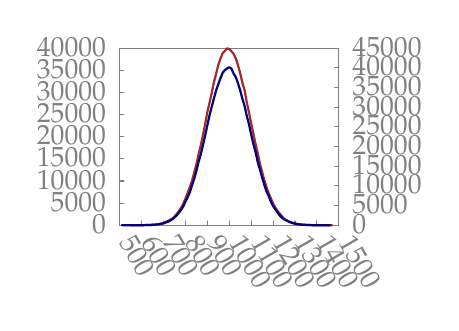
\begin{tikzpicture}[gnuplot, scale=0.3]
%% generated with GNUPLOT 5.2p2 (Lua 5.3; terminal rev. 99, script rev. 102)
%% wo 11 jul 2018 09:51:59 CEST
\path (0.000,0.000) rectangle (12.500,8.750);
\gpcolor{rgb color={0.502,0.502,0.502}}
\gpsetlinetype{gp lt border}
\gpsetdashtype{gp dt solid}
\gpsetlinewidth{1.00}
\draw[gp path] (1.380,0.945)--(1.560,0.945);
\node[gp node right] at (1.196,0.945) {$0$};
\draw[gp path] (1.380,1.882)--(1.560,1.882);
\node[gp node right] at (1.196,1.882) {$5000$};
\draw[gp path] (1.380,2.819)--(1.560,2.819);
\node[gp node right] at (1.196,2.819) {$10000$};
\draw[gp path] (1.380,3.756)--(1.560,3.756);
\node[gp node right] at (1.196,3.756) {$15000$};
\draw[gp path] (1.380,4.693)--(1.560,4.693);
\node[gp node right] at (1.196,4.693) {$20000$};
\draw[gp path] (1.380,5.630)--(1.560,5.630);
\node[gp node right] at (1.196,5.630) {$25000$};
\draw[gp path] (1.380,6.567)--(1.560,6.567);
\node[gp node right] at (1.196,6.567) {$30000$};
\draw[gp path] (1.380,7.504)--(1.560,7.504);
\node[gp node right] at (1.196,7.504) {$35000$};
\draw[gp path] (1.380,8.441)--(1.560,8.441);
\node[gp node right] at (1.196,8.441) {$40000$};
\draw[gp path] (1.380,0.945)--(1.380,1.125);
\node[gp node left,rotate=-60] at (1.380,0.761) {$500$};
\draw[gp path] (2.308,0.945)--(2.308,1.125);
\node[gp node left,rotate=-60] at (2.308,0.761) {$600$};
\draw[gp path] (3.236,0.945)--(3.236,1.125);
\node[gp node left,rotate=-60] at (3.236,0.761) {$700$};
\draw[gp path] (4.164,0.945)--(4.164,1.125);
\node[gp node left,rotate=-60] at (4.164,0.761) {$800$};
\draw[gp path] (5.092,0.945)--(5.092,1.125);
\node[gp node left,rotate=-60] at (5.092,0.761) {$900$};
\draw[gp path] (6.020,0.945)--(6.020,1.125);
\node[gp node left,rotate=-60] at (6.020,0.761) {$1000$};
\draw[gp path] (6.947,0.945)--(6.947,1.125);
\node[gp node left,rotate=-60] at (6.947,0.761) {$1100$};
\draw[gp path] (7.875,0.945)--(7.875,1.125);
\node[gp node left,rotate=-60] at (7.875,0.761) {$1200$};
\draw[gp path] (8.803,0.945)--(8.803,1.125);
\node[gp node left,rotate=-60] at (8.803,0.761) {$1300$};
\draw[gp path] (9.731,0.945)--(9.731,1.125);
\node[gp node left,rotate=-60] at (9.731,0.761) {$1400$};
\draw[gp path] (10.659,0.945)--(10.659,1.125);
\node[gp node left,rotate=-60] at (10.659,0.761) {$1500$};
\draw[gp path] (10.659,0.945)--(10.479,0.945);
\node[gp node left] at (10.843,0.945) {$0$};
\draw[gp path] (10.659,1.778)--(10.479,1.778);
\node[gp node left] at (10.843,1.778) {$5000$};
\draw[gp path] (10.659,2.611)--(10.479,2.611);
\node[gp node left] at (10.843,2.611) {$10000$};
\draw[gp path] (10.659,3.444)--(10.479,3.444);
\node[gp node left] at (10.843,3.444) {$15000$};
\draw[gp path] (10.659,4.277)--(10.479,4.277);
\node[gp node left] at (10.843,4.277) {$20000$};
\draw[gp path] (10.659,5.109)--(10.479,5.109);
\node[gp node left] at (10.843,5.109) {$25000$};
\draw[gp path] (10.659,5.942)--(10.479,5.942);
\node[gp node left] at (10.843,5.942) {$30000$};
\draw[gp path] (10.659,6.775)--(10.479,6.775);
\node[gp node left] at (10.843,6.775) {$35000$};
\draw[gp path] (10.659,7.608)--(10.479,7.608);
\node[gp node left] at (10.843,7.608) {$40000$};
\draw[gp path] (10.659,8.441)--(10.479,8.441);
\node[gp node left] at (10.843,8.441) {$45000$};
\draw[gp path] (1.380,8.441)--(1.380,0.945)--(10.659,0.945)--(10.659,8.441)--cycle;
\gpcolor{rgb color={0.647,0.165,0.165}}
\gpsetlinewidth{2.00}
\draw[gp path] (1.844,0.946)--(1.937,0.945)--(2.030,0.946)--(2.122,0.946)--(2.215,0.948)%
  --(2.308,0.948)--(2.401,0.949)--(2.493,0.951)--(2.586,0.953)--(2.679,0.959)--(2.772,0.966)%
  --(2.865,0.971)--(2.957,0.980)--(3.050,0.994)--(3.143,1.013)--(3.236,1.037)--(3.329,1.086)%
  --(3.421,1.123)--(3.514,1.175)--(3.607,1.224)--(3.700,1.304)--(3.793,1.418)--(3.885,1.544)%
  --(3.978,1.675)--(4.071,1.846)--(4.164,2.071)--(4.256,2.307)--(4.349,2.556)--(4.442,2.820)%
  --(4.535,3.179)--(4.628,3.517)--(4.720,3.952)--(4.813,4.322)--(4.906,4.752)--(4.999,5.220)%
  --(5.092,5.739)--(5.184,6.123)--(5.277,6.542)--(5.370,6.994)--(5.463,7.357)--(5.556,7.733)%
  --(5.648,7.999)--(5.741,8.233)--(5.834,8.320)--(5.927,8.434)--(6.020,8.407)--(6.112,8.309)%
  --(6.205,8.194)--(6.298,7.999)--(6.391,7.715)--(6.483,7.381)--(6.576,6.970)--(6.669,6.659)%
  --(6.762,6.144)--(6.855,5.726)--(6.947,5.260)--(7.040,4.822)--(7.133,4.379)--(7.226,3.990)%
  --(7.319,3.556)--(7.411,3.198)--(7.504,2.858)--(7.597,2.552)--(7.690,2.296)--(7.783,2.082)%
  --(7.875,1.860)--(7.968,1.693)--(8.061,1.552)--(8.154,1.442)--(8.246,1.334)--(8.339,1.225)%
  --(8.432,1.167)--(8.525,1.109)--(8.618,1.080)--(8.710,1.036)--(8.803,1.020)--(8.896,0.999)%
  --(8.989,0.984)--(9.082,0.975)--(9.174,0.963)--(9.267,0.962)--(9.360,0.956)--(9.453,0.953)%
  --(9.546,0.949)--(9.638,0.949)--(9.731,0.948)--(9.824,0.946)--(9.917,0.947)--(10.009,0.946)%
  --(10.102,0.945)--(10.195,0.945)--(10.288,0.945)--(10.381,0.945);
\gpcolor{rgb color={0.000,0.000,0.502}}
\draw[gp path] (1.473,0.945)--(1.844,0.945)--(1.937,0.945)--(2.030,0.945)--(2.122,0.946)%
  --(2.215,0.948)--(2.308,0.949)--(2.401,0.949)--(2.493,0.951)--(2.586,0.953)--(2.679,0.955)%
  --(2.772,0.962)--(2.865,0.969)--(2.957,0.978)--(3.050,0.990)--(3.143,1.013)--(3.236,1.025)%
  --(3.329,1.061)--(3.421,1.092)--(3.514,1.139)--(3.607,1.196)--(3.700,1.277)--(3.793,1.364)%
  --(3.885,1.470)--(3.978,1.590)--(4.071,1.742)--(4.164,1.935)--(4.256,2.124)--(4.349,2.338)%
  --(4.442,2.629)--(4.535,2.904)--(4.628,3.239)--(4.720,3.628)--(4.813,3.940)--(4.906,4.327)%
  --(4.999,4.738)--(5.092,5.177)--(5.184,5.596)--(5.277,5.960)--(5.370,6.309)--(5.463,6.652)%
  --(5.556,6.918)--(5.648,7.168)--(5.741,7.401)--(5.834,7.508)--(5.927,7.584)--(6.020,7.633)%
  --(6.112,7.575)--(6.205,7.365)--(6.298,7.215)--(6.391,6.946)--(6.483,6.656)--(6.576,6.302)%
  --(6.669,5.995)--(6.762,5.569)--(6.855,5.221)--(6.947,4.791)--(7.040,4.387)--(7.133,4.048)%
  --(7.226,3.615)--(7.319,3.302)--(7.411,2.969)--(7.504,2.655)--(7.597,2.378)--(7.690,2.178)%
  --(7.783,1.940)--(7.875,1.758)--(7.968,1.625)--(8.061,1.487)--(8.154,1.360)--(8.246,1.267)%
  --(8.339,1.199)--(8.432,1.153)--(8.525,1.104)--(8.618,1.064)--(8.710,1.036)--(8.803,1.011)%
  --(8.896,0.991)--(8.989,0.980)--(9.082,0.969)--(9.174,0.964)--(9.267,0.959)--(9.360,0.954)%
  --(9.453,0.950)--(9.546,0.948)--(9.638,0.947)--(9.731,0.947)--(9.824,0.946)--(9.917,0.945)%
  --(10.009,0.945)--(10.102,0.945)--(10.195,0.945)--(10.288,0.945);
%% coordinates of the plot area
\gpdefrectangularnode{gp plot 1}{\pgfpoint{1.380cm}{0.945cm}}{\pgfpoint{10.659cm}{8.441cm}}
\end{tikzpicture}
%% gnuplot variables

\end{tabular}
\end{center}
\caption{\label{fig:inputselection:normal_1to1_randomOn}
  Same deposits and withdrawals as in
  Figure~\ref{fig:inputselection:normal_1to1_randomOff}, but now using the
  ``pick randomly until we have a change output roughly equal to the payment''
  algorithm.
}
\end{figure}

Note that the UTxO now follows precisely the distribution of payment requests,
and we're not generating dust anymore. One advantage of this is that because
we have no dust, the average number of inputs per transaction can be lower
than in the basic algorithm.

Just to illustrate this again,
Figure~\ref{fig:inputselection:normal_3to1_randomOn} shows the result of the
algorithm but now with a 3:1 ratio of deposits and withdrawals. We have two
bumps now: one normally distributed around 1000, corresponding to the the
deposits, and one normally distributed around 3000, corresponding to the payment
requests that are being made. As before, the median change:payment ratio is a
satisfying round 1.0.

\begin{figure}[p]
\begin{center}
\scriptsize
\begin{tabular}{ll}
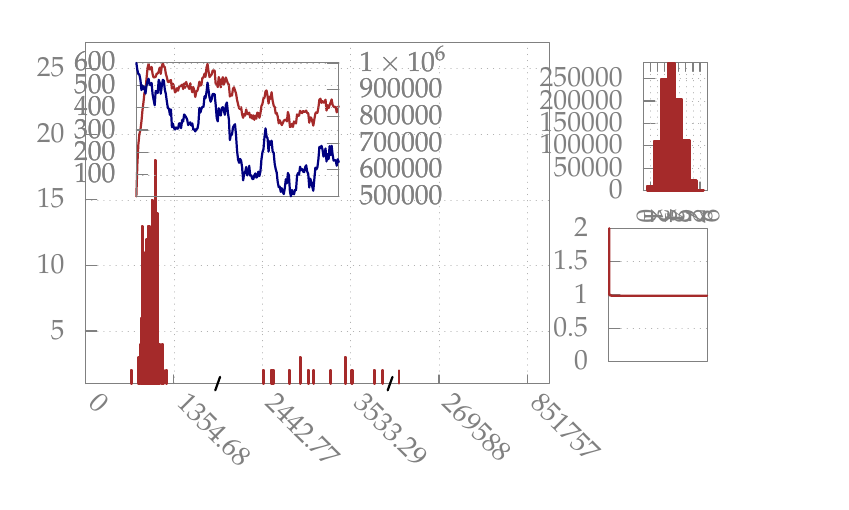
\begin{tikzpicture}[gnuplot, xscale=0.8, yscale=0.6]
%% generated with GNUPLOT 5.2p2 (Lua 5.3; terminal rev. 99, script rev. 102)
%% wo 11 jul 2018 10:46:24 CEST
\path (0.000,0.000) rectangle (12.500,8.750);
\gpcolor{color=gp lt color axes}
\gpsetlinetype{gp lt axes}
\gpsetdashtype{gp dt axes}
\gpsetlinewidth{0.50}
\draw[gp path] (0.828,2.329)--(8.197,2.329);
\gpcolor{rgb color={0.502,0.502,0.502}}
\gpsetlinetype{gp lt border}
\gpsetdashtype{gp dt solid}
\gpsetlinewidth{1.00}
\draw[gp path] (0.828,2.329)--(1.008,2.329);
\node[gp node right] at (0.644,2.329) {$5$};
\gpcolor{color=gp lt color axes}
\gpsetlinetype{gp lt axes}
\gpsetdashtype{gp dt axes}
\gpsetlinewidth{0.50}
\draw[gp path] (0.828,3.718)--(8.197,3.718);
\gpcolor{rgb color={0.502,0.502,0.502}}
\gpsetlinetype{gp lt border}
\gpsetdashtype{gp dt solid}
\gpsetlinewidth{1.00}
\draw[gp path] (0.828,3.718)--(1.008,3.718);
\node[gp node right] at (0.644,3.718) {$10$};
\gpcolor{color=gp lt color axes}
\gpsetlinetype{gp lt axes}
\gpsetdashtype{gp dt axes}
\gpsetlinewidth{0.50}
\draw[gp path] (0.828,5.107)--(8.197,5.107);
\gpcolor{rgb color={0.502,0.502,0.502}}
\gpsetlinetype{gp lt border}
\gpsetdashtype{gp dt solid}
\gpsetlinewidth{1.00}
\draw[gp path] (0.828,5.107)--(1.008,5.107);
\node[gp node right] at (0.644,5.107) {$15$};
\gpcolor{color=gp lt color axes}
\gpsetlinetype{gp lt axes}
\gpsetdashtype{gp dt axes}
\gpsetlinewidth{0.50}
\draw[gp path] (0.828,6.496)--(8.197,6.496);
\gpcolor{rgb color={0.502,0.502,0.502}}
\gpsetlinetype{gp lt border}
\gpsetdashtype{gp dt solid}
\gpsetlinewidth{1.00}
\draw[gp path] (0.828,6.496)--(1.008,6.496);
\node[gp node right] at (0.644,6.496) {$20$};
\gpcolor{color=gp lt color axes}
\gpsetlinetype{gp lt axes}
\gpsetdashtype{gp dt axes}
\gpsetlinewidth{0.50}
\draw[gp path] (0.828,7.885)--(8.197,7.885);
\gpcolor{rgb color={0.502,0.502,0.502}}
\gpsetlinetype{gp lt border}
\gpsetdashtype{gp dt solid}
\gpsetlinewidth{1.00}
\draw[gp path] (0.828,7.885)--(1.008,7.885);
\node[gp node right] at (0.644,7.885) {$25$};
\gpcolor{color=gp lt color axes}
\gpsetlinetype{gp lt axes}
\gpsetdashtype{gp dt axes}
\gpsetlinewidth{0.50}
\draw[gp path] (0.828,1.218)--(0.828,8.441);
\gpcolor{rgb color={0.502,0.502,0.502}}
\gpsetlinetype{gp lt border}
\gpsetdashtype{gp dt solid}
\gpsetlinewidth{1.00}
\draw[gp path] (0.828,1.218)--(0.828,1.398);
\node[gp node left,rotate=-45] at (0.828,1.034) {$0$};
\gpcolor{color=gp lt color axes}
\gpsetlinetype{gp lt axes}
\gpsetdashtype{gp dt axes}
\gpsetlinewidth{0.50}
\draw[gp path] (2.232,1.218)--(2.232,8.441);
\gpcolor{rgb color={0.502,0.502,0.502}}
\gpsetlinetype{gp lt border}
\gpsetdashtype{gp dt solid}
\gpsetlinewidth{1.00}
\draw[gp path] (2.232,1.218)--(2.232,1.398);
\node[gp node left,rotate=-45] at (2.232,1.034) {$1354.68$};
\gpcolor{color=gp lt color axes}
\gpsetlinetype{gp lt axes}
\gpsetdashtype{gp dt axes}
\gpsetlinewidth{0.50}
\draw[gp path] (3.635,1.218)--(3.635,8.441);
\gpcolor{rgb color={0.502,0.502,0.502}}
\gpsetlinetype{gp lt border}
\gpsetdashtype{gp dt solid}
\gpsetlinewidth{1.00}
\draw[gp path] (3.635,1.218)--(3.635,1.398);
\node[gp node left,rotate=-45] at (3.635,1.034) {$2442.77$};
\gpcolor{color=gp lt color axes}
\gpsetlinetype{gp lt axes}
\gpsetdashtype{gp dt axes}
\gpsetlinewidth{0.50}
\draw[gp path] (5.039,1.218)--(5.039,8.441);
\gpcolor{rgb color={0.502,0.502,0.502}}
\gpsetlinetype{gp lt border}
\gpsetdashtype{gp dt solid}
\gpsetlinewidth{1.00}
\draw[gp path] (5.039,1.218)--(5.039,1.398);
\node[gp node left,rotate=-45] at (5.039,1.034) {$3533.29$};
\gpcolor{color=gp lt color axes}
\gpsetlinetype{gp lt axes}
\gpsetdashtype{gp dt axes}
\gpsetlinewidth{0.50}
\draw[gp path] (6.442,1.218)--(6.442,8.441);
\gpcolor{rgb color={0.502,0.502,0.502}}
\gpsetlinetype{gp lt border}
\gpsetdashtype{gp dt solid}
\gpsetlinewidth{1.00}
\draw[gp path] (6.442,1.218)--(6.442,1.398);
\node[gp node left,rotate=-45] at (6.442,1.034) {$269588$};
\gpcolor{color=gp lt color axes}
\gpsetlinetype{gp lt axes}
\gpsetdashtype{gp dt axes}
\gpsetlinewidth{0.50}
\draw[gp path] (7.846,1.218)--(7.846,8.261)--(7.846,8.441);
\gpcolor{rgb color={0.502,0.502,0.502}}
\gpsetlinetype{gp lt border}
\gpsetdashtype{gp dt solid}
\gpsetlinewidth{1.00}
\draw[gp path] (7.846,1.218)--(7.846,1.398);
\node[gp node left,rotate=-45] at (7.846,1.034) {$851757$};
\draw[gp path] (0.828,8.441)--(0.828,1.218)--(8.197,1.218)--(8.197,8.441)--cycle;
\gpcolor{rgb color={0.647,0.165,0.165}}
\gpsetlinewidth{2.00}
\draw[gp path] (1.558,1.218)--(1.558,1.496)--(1.569,1.496)--(1.569,1.218)--cycle;
\draw[gp path] (1.662,1.218)--(1.662,1.496)--(1.672,1.496)--(1.672,1.218)--cycle;
\draw[gp path] (1.672,1.218)--(1.672,1.774)--(1.683,1.774)--(1.683,1.218)--cycle;
\draw[gp path] (1.683,1.218)--(1.683,1.774)--(1.693,1.774)--(1.693,1.218)--cycle;
\draw[gp path] (1.704,1.218)--(1.704,2.051)--(1.714,2.051)--(1.714,1.218)--cycle;
\draw[gp path] (1.714,1.218)--(1.714,2.607)--(1.724,2.607)--(1.724,1.218)--cycle;
\draw[gp path] (1.724,1.218)--(1.724,4.552)--(1.735,4.552)--(1.735,1.218)--cycle;
\draw[gp path] (1.735,1.218)--(1.735,2.329)--(1.745,2.329)--(1.745,1.218)--cycle;
\draw[gp path] (1.745,1.218)--(1.745,3.996)--(1.755,3.996)--(1.755,1.218)--cycle;
\draw[gp path] (1.755,1.218)--(1.755,2.051)--(1.766,2.051)--(1.766,1.218)--cycle;
\draw[gp path] (1.766,1.218)--(1.766,3.718)--(1.776,3.718)--(1.776,1.218)--cycle;
\draw[gp path] (1.776,1.218)--(1.776,1.774)--(1.786,1.774)--(1.786,1.218)--cycle;
\draw[gp path] (1.786,1.218)--(1.786,3.163)--(1.797,3.163)--(1.797,1.218)--cycle;
\draw[gp path] (1.797,1.218)--(1.797,4.274)--(1.807,4.274)--(1.807,1.218)--cycle;
\draw[gp path] (1.807,1.218)--(1.807,2.885)--(1.817,2.885)--(1.817,1.218)--cycle;
\draw[gp path] (1.817,1.218)--(1.817,3.440)--(1.828,3.440)--(1.828,1.218)--cycle;
\draw[gp path] (1.828,1.218)--(1.828,4.552)--(1.838,4.552)--(1.838,1.218)--cycle;
\draw[gp path] (1.838,1.218)--(1.838,4.552)--(1.849,4.552)--(1.849,1.218)--cycle;
\draw[gp path] (1.849,1.218)--(1.849,3.996)--(1.859,3.996)--(1.859,1.218)--cycle;
\draw[gp path] (1.859,1.218)--(1.859,3.996)--(1.869,3.996)--(1.869,1.218)--cycle;
\draw[gp path] (1.869,1.218)--(1.869,3.440)--(1.880,3.440)--(1.880,1.218)--cycle;
\draw[gp path] (1.880,1.218)--(1.880,5.107)--(1.890,5.107)--(1.890,1.218)--cycle;
\draw[gp path] (1.890,1.218)--(1.890,5.107)--(1.900,5.107)--(1.900,1.218)--cycle;
\draw[gp path] (1.900,1.218)--(1.900,3.718)--(1.911,3.718)--(1.911,1.218)--cycle;
\draw[gp path] (1.911,1.218)--(1.911,3.718)--(1.921,3.718)--(1.921,1.218)--cycle;
\draw[gp path] (1.921,1.218)--(1.921,2.885)--(1.931,2.885)--(1.931,1.218)--cycle;
\draw[gp path] (1.931,1.218)--(1.931,5.941)--(1.942,5.941)--(1.942,1.218)--cycle;
\draw[gp path] (1.942,1.218)--(1.942,2.607)--(1.952,2.607)--(1.952,1.218)--cycle;
\draw[gp path] (1.952,1.218)--(1.952,2.885)--(1.963,2.885)--(1.963,1.218)--cycle;
\draw[gp path] (1.963,1.218)--(1.963,4.830)--(1.973,4.830)--(1.973,1.218)--cycle;
\draw[gp path] (1.973,1.218)--(1.973,2.885)--(1.983,2.885)--(1.983,1.218)--cycle;
\draw[gp path] (1.983,1.218)--(1.983,1.496)--(1.994,1.496)--(1.994,1.218)--cycle;
\draw[gp path] (1.994,1.218)--(1.994,2.051)--(2.004,2.051)--(2.004,1.218)--cycle;
\draw[gp path] (2.004,1.218)--(2.004,2.051)--(2.014,2.051)--(2.014,1.218)--cycle;
\draw[gp path] (2.025,1.218)--(2.025,1.496)--(2.035,1.496)--(2.035,1.218)--cycle;
\draw[gp path] (2.045,1.218)--(2.045,2.051)--(2.056,2.051)--(2.056,1.218)--cycle;
\draw[gp path] (2.066,1.218)--(2.066,1.496)--(2.077,1.496)--(2.077,1.218)--cycle;
\draw[gp path] (2.108,1.218)--(2.108,1.496)--(2.118,1.496)--(2.118,1.218)--cycle;
\draw[gp path] (3.651,1.218)--(3.651,1.496)--(3.664,1.496)--(3.664,1.218)--cycle;
\draw[gp path] (3.780,1.218)--(3.780,1.496)--(3.793,1.496)--(3.793,1.218)--cycle;
\draw[gp path] (3.793,1.218)--(3.793,1.496)--(3.805,1.496)--(3.805,1.218)--cycle;
\draw[gp path] (3.805,1.218)--(3.805,1.496)--(3.818,1.496)--(3.818,1.218)--cycle;
\draw[gp path] (4.063,1.218)--(4.063,1.496)--(4.076,1.496)--(4.076,1.218)--cycle;
\draw[gp path] (4.230,1.218)--(4.230,1.774)--(4.243,1.774)--(4.243,1.218)--cycle;
\draw[gp path] (4.359,1.218)--(4.359,1.496)--(4.372,1.496)--(4.372,1.218)--cycle;
\draw[gp path] (4.449,1.218)--(4.449,1.496)--(4.462,1.496)--(4.462,1.218)--cycle;
\draw[gp path] (4.719,1.218)--(4.719,1.496)--(4.732,1.496)--(4.732,1.218)--cycle;
\draw[gp path] (4.951,1.218)--(4.951,1.774)--(4.964,1.774)--(4.964,1.218)--cycle;
\draw[gp path] (5.054,1.218)--(5.054,1.496)--(5.067,1.496)--(5.067,1.218)--cycle;
\draw[gp path] (5.414,1.218)--(5.414,1.496)--(5.427,1.496)--(5.427,1.218)--cycle;
\draw[gp path] (5.543,1.218)--(5.543,1.496)--(5.556,1.496)--(5.556,1.218)--cycle;
\draw[gp path] (5.803,1.218)--(5.803,1.496)--cycle;
\gpcolor{color=gp lt color border}
\draw[gp path](2.890,1.074)--(2.966,1.358);
\draw[gp path](5.627,1.074)--(5.703,1.358);
%% coordinates of the plot area
\gpdefrectangularnode{gp plot 1}{\pgfpoint{0.828cm}{1.218cm}}{\pgfpoint{8.197cm}{8.441cm}}
\gpcolor{color=gp lt color axes}
\gpsetlinetype{gp lt axes}
\gpsetdashtype{gp dt axes}
\gpsetlinewidth{0.50}
\draw[gp path] (1.637,5.635)--(4.850,5.635);
\gpcolor{rgb color={0.502,0.502,0.502}}
\gpsetlinetype{gp lt border}
\gpsetdashtype{gp dt solid}
\gpsetlinewidth{1.00}
\draw[gp path] (1.637,5.635)--(1.817,5.635);
\node[gp node right] at (1.453,5.635) {$100$};
\gpcolor{color=gp lt color axes}
\gpsetlinetype{gp lt axes}
\gpsetdashtype{gp dt axes}
\gpsetlinewidth{0.50}
\draw[gp path] (1.637,6.109)--(4.850,6.109);
\gpcolor{rgb color={0.502,0.502,0.502}}
\gpsetlinetype{gp lt border}
\gpsetdashtype{gp dt solid}
\gpsetlinewidth{1.00}
\draw[gp path] (1.637,6.109)--(1.817,6.109);
\node[gp node right] at (1.453,6.109) {$200$};
\gpcolor{color=gp lt color axes}
\gpsetlinetype{gp lt axes}
\gpsetdashtype{gp dt axes}
\gpsetlinewidth{0.50}
\draw[gp path] (1.637,6.583)--(4.850,6.583);
\gpcolor{rgb color={0.502,0.502,0.502}}
\gpsetlinetype{gp lt border}
\gpsetdashtype{gp dt solid}
\gpsetlinewidth{1.00}
\draw[gp path] (1.637,6.583)--(1.817,6.583);
\node[gp node right] at (1.453,6.583) {$300$};
\gpcolor{color=gp lt color axes}
\gpsetlinetype{gp lt axes}
\gpsetdashtype{gp dt axes}
\gpsetlinewidth{0.50}
\draw[gp path] (1.637,7.056)--(4.850,7.056);
\gpcolor{rgb color={0.502,0.502,0.502}}
\gpsetlinetype{gp lt border}
\gpsetdashtype{gp dt solid}
\gpsetlinewidth{1.00}
\draw[gp path] (1.637,7.056)--(1.817,7.056);
\node[gp node right] at (1.453,7.056) {$400$};
\gpcolor{color=gp lt color axes}
\gpsetlinetype{gp lt axes}
\gpsetdashtype{gp dt axes}
\gpsetlinewidth{0.50}
\draw[gp path] (1.637,7.530)--(4.850,7.530);
\gpcolor{rgb color={0.502,0.502,0.502}}
\gpsetlinetype{gp lt border}
\gpsetdashtype{gp dt solid}
\gpsetlinewidth{1.00}
\draw[gp path] (1.637,7.530)--(1.817,7.530);
\node[gp node right] at (1.453,7.530) {$500$};
\gpcolor{color=gp lt color axes}
\gpsetlinetype{gp lt axes}
\gpsetdashtype{gp dt axes}
\gpsetlinewidth{0.50}
\draw[gp path] (1.637,8.004)--(4.850,8.004);
\gpcolor{rgb color={0.502,0.502,0.502}}
\gpsetlinetype{gp lt border}
\gpsetdashtype{gp dt solid}
\gpsetlinewidth{1.00}
\draw[gp path] (1.637,8.004)--(1.817,8.004);
\node[gp node right] at (1.453,8.004) {$600$};
\draw[gp path] (4.850,5.177)--(4.670,5.177);
\node[gp node left] at (5.034,5.177) {$500000$};
\draw[gp path] (4.850,5.742)--(4.670,5.742);
\node[gp node left] at (5.034,5.742) {$600000$};
\draw[gp path] (4.850,6.307)--(4.670,6.307);
\node[gp node left] at (5.034,6.307) {$700000$};
\draw[gp path] (4.850,6.872)--(4.670,6.872);
\node[gp node left] at (5.034,6.872) {$800000$};
\draw[gp path] (4.850,7.437)--(4.670,7.437);
\node[gp node left] at (5.034,7.437) {$900000$};
\draw[gp path] (4.850,8.003)--(4.670,8.003);
\node[gp node left] at (5.034,8.003) {$1\times10^{6}$};
\draw[gp path] (1.637,8.004)--(1.637,5.180)--(4.850,5.180)--(4.850,8.004)--cycle;
\gpcolor{rgb color={0.647,0.165,0.165}}
\gpsetlinewidth{2.00}
\draw[gp path] (1.637,5.180)--(1.653,5.858)--(1.669,6.279)--(1.685,6.497)--(1.702,6.587)%
  --(1.718,6.767)--(1.734,6.999)--(1.750,7.170)--(1.766,7.374)--(1.782,7.412)--(1.798,7.668)%
  --(1.815,7.895)--(1.831,7.985)--(1.847,7.867)--(1.863,7.871)--(1.879,7.919)--(1.895,7.767)%
  --(1.911,7.696)--(1.928,7.701)--(1.944,7.710)--(1.960,7.777)--(1.976,7.781)--(1.992,7.819)%
  --(2.008,7.904)--(2.024,7.772)--(2.041,7.928)--(2.057,8.004)--(2.073,7.928)--(2.089,7.914)%
  --(2.105,7.777)--(2.121,7.701)--(2.138,7.601)--(2.154,7.601)--(2.170,7.630)--(2.186,7.639)%
  --(2.202,7.459)--(2.218,7.563)--(2.234,7.497)--(2.251,7.379)--(2.267,7.407)--(2.283,7.469)%
  --(2.299,7.416)--(2.315,7.492)--(2.331,7.521)--(2.347,7.516)--(2.364,7.544)--(2.380,7.450)%
  --(2.396,7.568)--(2.412,7.478)--(2.428,7.601)--(2.444,7.525)--(2.460,7.502)--(2.477,7.454)%
  --(2.493,7.573)--(2.509,7.473)--(2.525,7.383)--(2.541,7.492)--(2.557,7.416)--(2.573,7.284)%
  --(2.590,7.402)--(2.606,7.416)--(2.622,7.492)--(2.638,7.606)--(2.654,7.525)--(2.670,7.544)%
  --(2.686,7.691)--(2.703,7.696)--(2.719,7.777)--(2.735,7.710)--(2.751,7.904)--(2.767,7.985)%
  --(2.783,7.824)--(2.799,7.705)--(2.816,7.734)--(2.832,7.758)--(2.848,7.838)--(2.864,7.848)%
  --(2.880,7.838)--(2.896,7.563)--(2.913,7.568)--(2.929,7.492)--(2.945,7.705)--(2.961,7.639)%
  --(2.977,7.488)--(2.993,7.639)--(3.009,7.701)--(3.026,7.544)--(3.042,7.611)--(3.058,7.696)%
  --(3.074,7.630)--(3.090,7.568)--(3.106,7.544)--(3.122,7.293)--(3.139,7.336)--(3.155,7.312)%
  --(3.171,7.454)--(3.187,7.488)--(3.203,7.421)--(3.219,7.360)--(3.235,7.227)--(3.252,7.127)%
  --(3.268,7.047)--(3.284,7.028)--(3.300,7.066)--(3.316,6.914)--(3.332,6.843)--(3.348,6.924)%
  --(3.365,6.891)--(3.381,7.018)--(3.397,6.924)--(3.413,6.924)--(3.429,6.952)--(3.445,6.848)%
  --(3.461,6.900)--(3.478,6.824)--(3.494,6.895)--(3.510,6.800)--(3.526,6.886)--(3.542,6.824)%
  --(3.558,6.952)--(3.574,6.938)--(3.591,6.843)--(3.607,6.938)--(3.623,7.094)--(3.639,7.137)%
  --(3.655,7.255)--(3.671,7.265)--(3.688,7.402)--(3.704,7.421)--(3.720,7.303)--(3.736,7.146)%
  --(3.752,7.289)--(3.768,7.246)--(3.784,7.383)--(3.801,7.203)--(3.817,7.099)--(3.833,7.071)%
  --(3.849,6.933)--(3.865,6.947)--(3.881,6.872)--(3.897,6.725)--(3.914,6.791)--(3.930,6.739)%
  --(3.946,6.687)--(3.962,6.729)--(3.978,6.782)--(3.994,6.796)--(4.010,6.805)--(4.027,6.767)%
  --(4.043,6.966)--(4.059,6.881)--(4.075,6.649)--(4.091,6.654)--(4.107,6.715)--(4.123,6.649)%
  --(4.140,6.763)--(4.156,6.739)--(4.172,6.725)--(4.188,6.914)--(4.204,6.886)--(4.220,6.886)%
  --(4.236,6.990)--(4.253,6.957)--(4.269,6.943)--(4.285,6.985)--(4.301,6.971)--(4.317,6.971)%
  --(4.333,6.995)--(4.349,6.943)--(4.366,6.938)--(4.382,6.739)--(4.398,6.853)--(4.414,6.838)%
  --(4.430,6.763)--(4.446,6.677)--(4.463,6.815)--(4.479,6.933)--(4.495,6.962)--(4.511,6.947)%
  --(4.527,7.061)--(4.543,7.227)--(4.559,7.246)--(4.576,7.161)--(4.592,7.194)--(4.608,7.165)%
  --(4.624,7.165)--(4.640,7.227)--(4.656,6.995)--(4.672,7.108)--(4.689,7.047)--(4.705,7.113)%
  --(4.721,7.165)--(4.737,7.232)--(4.753,7.113)--(4.769,7.080)--(4.785,7.066)--(4.802,7.071)%
  --(4.818,6.957)--(4.834,7.056)--(4.850,7.085);
%% coordinates of the plot area
\gpdefrectangularnode{gp plot 2}{\pgfpoint{1.637cm}{5.180cm}}{\pgfpoint{4.850cm}{8.004cm}}
\gpcolor{color=gp lt color axes}
\gpsetlinetype{gp lt axes}
\gpsetdashtype{gp dt axes}
\gpsetlinewidth{0.50}
\draw[gp path] (1.637,5.635)--(4.850,5.635);
\gpcolor{rgb color={0.502,0.502,0.502}}
\gpsetlinetype{gp lt border}
\gpsetdashtype{gp dt solid}
\gpsetlinewidth{1.00}
\draw[gp path] (1.637,5.635)--(1.817,5.635);
\node[gp node right] at (1.453,5.635) {$100$};
\gpcolor{color=gp lt color axes}
\gpsetlinetype{gp lt axes}
\gpsetdashtype{gp dt axes}
\gpsetlinewidth{0.50}
\draw[gp path] (1.637,6.109)--(4.850,6.109);
\gpcolor{rgb color={0.502,0.502,0.502}}
\gpsetlinetype{gp lt border}
\gpsetdashtype{gp dt solid}
\gpsetlinewidth{1.00}
\draw[gp path] (1.637,6.109)--(1.817,6.109);
\node[gp node right] at (1.453,6.109) {$200$};
\gpcolor{color=gp lt color axes}
\gpsetlinetype{gp lt axes}
\gpsetdashtype{gp dt axes}
\gpsetlinewidth{0.50}
\draw[gp path] (1.637,6.583)--(4.850,6.583);
\gpcolor{rgb color={0.502,0.502,0.502}}
\gpsetlinetype{gp lt border}
\gpsetdashtype{gp dt solid}
\gpsetlinewidth{1.00}
\draw[gp path] (1.637,6.583)--(1.817,6.583);
\node[gp node right] at (1.453,6.583) {$300$};
\gpcolor{color=gp lt color axes}
\gpsetlinetype{gp lt axes}
\gpsetdashtype{gp dt axes}
\gpsetlinewidth{0.50}
\draw[gp path] (1.637,7.056)--(4.850,7.056);
\gpcolor{rgb color={0.502,0.502,0.502}}
\gpsetlinetype{gp lt border}
\gpsetdashtype{gp dt solid}
\gpsetlinewidth{1.00}
\draw[gp path] (1.637,7.056)--(1.817,7.056);
\node[gp node right] at (1.453,7.056) {$400$};
\gpcolor{color=gp lt color axes}
\gpsetlinetype{gp lt axes}
\gpsetdashtype{gp dt axes}
\gpsetlinewidth{0.50}
\draw[gp path] (1.637,7.530)--(4.850,7.530);
\gpcolor{rgb color={0.502,0.502,0.502}}
\gpsetlinetype{gp lt border}
\gpsetdashtype{gp dt solid}
\gpsetlinewidth{1.00}
\draw[gp path] (1.637,7.530)--(1.817,7.530);
\node[gp node right] at (1.453,7.530) {$500$};
\gpcolor{color=gp lt color axes}
\gpsetlinetype{gp lt axes}
\gpsetdashtype{gp dt axes}
\gpsetlinewidth{0.50}
\draw[gp path] (1.637,8.004)--(4.850,8.004);
\gpcolor{rgb color={0.502,0.502,0.502}}
\gpsetlinetype{gp lt border}
\gpsetdashtype{gp dt solid}
\gpsetlinewidth{1.00}
\draw[gp path] (1.637,8.004)--(1.817,8.004);
\node[gp node right] at (1.453,8.004) {$600$};
\draw[gp path] (4.850,5.177)--(4.670,5.177);
\node[gp node left] at (5.034,5.177) {$500000$};
\draw[gp path] (4.850,5.742)--(4.670,5.742);
\node[gp node left] at (5.034,5.742) {$600000$};
\draw[gp path] (4.850,6.307)--(4.670,6.307);
\node[gp node left] at (5.034,6.307) {$700000$};
\draw[gp path] (4.850,6.872)--(4.670,6.872);
\node[gp node left] at (5.034,6.872) {$800000$};
\draw[gp path] (4.850,7.437)--(4.670,7.437);
\node[gp node left] at (5.034,7.437) {$900000$};
\draw[gp path] (4.850,8.003)--(4.670,8.003);
\node[gp node left] at (5.034,8.003) {$1\times10^{6}$};
\draw[gp path] (1.637,8.004)--(1.637,5.180)--(4.850,5.180)--(4.850,8.004)--cycle;
\gpcolor{rgb color={0.000,0.000,0.502}}
\gpsetlinewidth{2.00}
\draw[gp path] (1.637,8.004)--(1.653,7.855)--(1.669,7.768)--(1.685,7.758)--(1.702,7.644)%
  --(1.718,7.429)--(1.734,7.525)--(1.750,7.450)--(1.766,7.490)--(1.782,7.354)--(1.798,7.522)%
  --(1.815,7.624)--(1.831,7.668)--(1.847,7.551)--(1.863,7.532)--(1.879,7.582)--(1.895,7.341)%
  --(1.911,7.224)--(1.928,7.108)--(1.944,7.409)--(1.960,7.402)--(1.976,7.366)--(1.992,7.646)%
  --(2.008,7.584)--(2.024,7.351)--(2.041,7.514)--(2.057,7.646)--(2.073,7.628)--(2.089,7.440)%
  --(2.105,7.348)--(2.121,7.189)--(2.138,7.045)--(2.154,7.039)--(2.170,6.904)--(2.186,7.021)%
  --(2.202,6.644)--(2.218,6.718)--(2.234,6.621)--(2.251,6.595)--(2.267,6.639)--(2.283,6.615)%
  --(2.299,6.611)--(2.315,6.725)--(2.331,6.723)--(2.347,6.623)--(2.364,6.796)--(2.380,6.764)%
  --(2.396,6.913)--(2.412,6.886)--(2.428,6.850)--(2.444,6.803)--(2.460,6.689)--(2.477,6.724)%
  --(2.493,6.746)--(2.509,6.681)--(2.525,6.723)--(2.541,6.594)--(2.557,6.601)--(2.573,6.554)%
  --(2.590,6.606)--(2.606,6.611)--(2.622,6.718)--(2.638,7.053)--(2.654,6.954)--(2.670,7.035)%
  --(2.686,7.074)--(2.703,7.073)--(2.719,7.297)--(2.735,7.262)--(2.751,7.390)--(2.767,7.587)%
  --(2.783,7.425)--(2.799,7.270)--(2.816,7.183)--(2.832,7.233)--(2.848,7.345)--(2.864,7.346)%
  --(2.880,7.341)--(2.896,7.121)--(2.913,6.837)--(2.929,6.767)--(2.945,7.045)--(2.961,6.970)%
  --(2.977,6.890)--(2.993,7.046)--(3.009,7.068)--(3.026,6.994)--(3.042,6.905)--(3.058,7.113)%
  --(3.074,7.167)--(3.090,6.959)--(3.106,6.808)--(3.122,6.372)--(3.139,6.493)--(3.155,6.486)%
  --(3.171,6.640)--(3.187,6.677)--(3.203,6.706)--(3.219,6.482)--(3.235,6.156)--(3.252,5.957)%
  --(3.268,5.890)--(3.284,5.972)--(3.300,5.935)--(3.316,5.794)--(3.332,5.518)--(3.348,5.651)%
  --(3.365,5.697)--(3.381,5.801)--(3.397,5.623)--(3.413,5.675)--(3.429,5.827)--(3.445,5.617)%
  --(3.461,5.625)--(3.478,5.548)--(3.494,5.544)--(3.510,5.626)--(3.526,5.666)--(3.542,5.577)%
  --(3.558,5.597)--(3.574,5.703)--(3.591,5.610)--(3.607,5.710)--(3.623,5.963)--(3.639,6.113)%
  --(3.655,6.176)--(3.671,6.432)--(3.688,6.619)--(3.704,6.447)--(3.720,6.410)--(3.736,6.125)%
  --(3.752,6.344)--(3.768,6.269)--(3.784,6.359)--(3.801,6.127)--(3.817,6.102)--(3.833,5.870)%
  --(3.849,5.757)--(3.865,5.684)--(3.881,5.483)--(3.897,5.375)--(3.914,5.385)--(3.930,5.275)%
  --(3.946,5.352)--(3.962,5.276)--(3.978,5.228)--(3.994,5.359)--(4.010,5.540)--(4.027,5.457)%
  --(4.043,5.673)--(4.059,5.625)--(4.075,5.284)--(4.091,5.180)--(4.107,5.316)--(4.123,5.237)%
  --(4.140,5.224)--(4.156,5.318)--(4.172,5.313)--(4.188,5.618)--(4.204,5.673)--(4.220,5.637)%
  --(4.236,5.807)--(4.253,5.737)--(4.269,5.754)--(4.285,5.703)--(4.301,5.694)--(4.317,5.793)%
  --(4.333,5.837)--(4.349,5.705)--(4.366,5.652)--(4.382,5.368)--(4.398,5.554)--(4.414,5.491)%
  --(4.430,5.386)--(4.446,5.298)--(4.463,5.551)--(4.479,5.787)--(4.495,5.751)--(4.511,5.794)%
  --(4.527,5.963)--(4.543,6.227)--(4.559,6.206)--(4.576,6.249)--(4.592,6.173)--(4.608,6.021)%
  --(4.624,6.054)--(4.640,6.194)--(4.656,5.919)--(4.672,6.072)--(4.689,5.966)--(4.705,6.242)%
  --(4.721,6.054)--(4.737,6.250)--(4.753,6.061)--(4.769,5.935)--(4.785,5.950)--(4.802,5.936)%
  --(4.818,5.828)--(4.834,5.965)--(4.850,5.904);
\gpcolor{color=gp lt color axes}
\gpsetlinetype{gp lt axes}
\gpsetdashtype{gp dt axes}
\gpsetlinewidth{0.50}
\draw[gp path] (9.688,5.304)--(10.697,5.304);
\gpcolor{rgb color={0.502,0.502,0.502}}
\gpsetlinetype{gp lt border}
\gpsetdashtype{gp dt solid}
\gpsetlinewidth{1.00}
\draw[gp path] (9.688,5.304)--(9.868,5.304);
\node[gp node right] at (9.504,5.304) {$0$};
\gpcolor{color=gp lt color axes}
\gpsetlinetype{gp lt axes}
\gpsetdashtype{gp dt axes}
\gpsetlinewidth{0.50}
\draw[gp path] (9.688,5.777)--(10.697,5.777);
\gpcolor{rgb color={0.502,0.502,0.502}}
\gpsetlinetype{gp lt border}
\gpsetdashtype{gp dt solid}
\gpsetlinewidth{1.00}
\draw[gp path] (9.688,5.777)--(9.868,5.777);
\node[gp node right] at (9.504,5.777) {$50000$};
\gpcolor{color=gp lt color axes}
\gpsetlinetype{gp lt axes}
\gpsetdashtype{gp dt axes}
\gpsetlinewidth{0.50}
\draw[gp path] (9.688,6.251)--(10.697,6.251);
\gpcolor{rgb color={0.502,0.502,0.502}}
\gpsetlinetype{gp lt border}
\gpsetdashtype{gp dt solid}
\gpsetlinewidth{1.00}
\draw[gp path] (9.688,6.251)--(9.868,6.251);
\node[gp node right] at (9.504,6.251) {$100000$};
\gpcolor{color=gp lt color axes}
\gpsetlinetype{gp lt axes}
\gpsetdashtype{gp dt axes}
\gpsetlinewidth{0.50}
\draw[gp path] (9.688,6.724)--(10.697,6.724);
\gpcolor{rgb color={0.502,0.502,0.502}}
\gpsetlinetype{gp lt border}
\gpsetdashtype{gp dt solid}
\gpsetlinewidth{1.00}
\draw[gp path] (9.688,6.724)--(9.868,6.724);
\node[gp node right] at (9.504,6.724) {$150000$};
\gpcolor{color=gp lt color axes}
\gpsetlinetype{gp lt axes}
\gpsetdashtype{gp dt axes}
\gpsetlinewidth{0.50}
\draw[gp path] (9.688,7.197)--(10.697,7.197);
\gpcolor{rgb color={0.502,0.502,0.502}}
\gpsetlinetype{gp lt border}
\gpsetdashtype{gp dt solid}
\gpsetlinewidth{1.00}
\draw[gp path] (9.688,7.197)--(9.868,7.197);
\node[gp node right] at (9.504,7.197) {$200000$};
\gpcolor{color=gp lt color axes}
\gpsetlinetype{gp lt axes}
\gpsetdashtype{gp dt axes}
\gpsetlinewidth{0.50}
\draw[gp path] (9.688,7.670)--(10.697,7.670);
\gpcolor{rgb color={0.502,0.502,0.502}}
\gpsetlinetype{gp lt border}
\gpsetdashtype{gp dt solid}
\gpsetlinewidth{1.00}
\draw[gp path] (9.688,7.670)--(9.868,7.670);
\node[gp node right] at (9.504,7.670) {$250000$};
\gpcolor{color=gp lt color axes}
\gpsetlinetype{gp lt axes}
\gpsetdashtype{gp dt axes}
\gpsetlinewidth{0.50}
\draw[gp path] (9.688,5.304)--(9.688,7.824)--(9.688,8.004);
\gpcolor{rgb color={0.502,0.502,0.502}}
\gpsetlinetype{gp lt border}
\gpsetdashtype{gp dt solid}
\gpsetlinewidth{1.00}
\draw[gp path] (9.688,5.304)--(9.688,5.484);
\draw[gp path] (9.688,8.004)--(9.688,7.824);
\node[gp node left,rotate=-90] at (9.688,5.120) {$0$};
\gpcolor{color=gp lt color axes}
\gpsetlinetype{gp lt axes}
\gpsetdashtype{gp dt axes}
\gpsetlinewidth{0.50}
\draw[gp path] (9.800,5.304)--(9.800,7.824)--(9.800,8.004);
\gpcolor{rgb color={0.502,0.502,0.502}}
\gpsetlinetype{gp lt border}
\gpsetdashtype{gp dt solid}
\gpsetlinewidth{1.00}
\draw[gp path] (9.800,5.304)--(9.800,5.484);
\draw[gp path] (9.800,8.004)--(9.800,7.824);
\node[gp node left,rotate=-90] at (9.800,5.120) {$1$};
\gpcolor{color=gp lt color axes}
\gpsetlinetype{gp lt axes}
\gpsetdashtype{gp dt axes}
\gpsetlinewidth{0.50}
\draw[gp path] (9.912,5.304)--(9.912,7.824)--(9.912,8.004);
\gpcolor{rgb color={0.502,0.502,0.502}}
\gpsetlinetype{gp lt border}
\gpsetdashtype{gp dt solid}
\gpsetlinewidth{1.00}
\draw[gp path] (9.912,5.304)--(9.912,5.484);
\draw[gp path] (9.912,8.004)--(9.912,7.824);
\node[gp node left,rotate=-90] at (9.912,5.120) {$2$};
\gpcolor{color=gp lt color axes}
\gpsetlinetype{gp lt axes}
\gpsetdashtype{gp dt axes}
\gpsetlinewidth{0.50}
\draw[gp path] (10.024,5.304)--(10.024,7.824)--(10.024,8.004);
\gpcolor{rgb color={0.502,0.502,0.502}}
\gpsetlinetype{gp lt border}
\gpsetdashtype{gp dt solid}
\gpsetlinewidth{1.00}
\draw[gp path] (10.024,5.304)--(10.024,5.484);
\draw[gp path] (10.024,8.004)--(10.024,7.824);
\node[gp node left,rotate=-90] at (10.024,5.120) {$3$};
\gpcolor{color=gp lt color axes}
\gpsetlinetype{gp lt axes}
\gpsetdashtype{gp dt axes}
\gpsetlinewidth{0.50}
\draw[gp path] (10.136,5.304)--(10.136,7.824)--(10.136,8.004);
\gpcolor{rgb color={0.502,0.502,0.502}}
\gpsetlinetype{gp lt border}
\gpsetdashtype{gp dt solid}
\gpsetlinewidth{1.00}
\draw[gp path] (10.136,5.304)--(10.136,5.484);
\draw[gp path] (10.136,8.004)--(10.136,7.824);
\node[gp node left,rotate=-90] at (10.136,5.120) {$4$};
\gpcolor{color=gp lt color axes}
\gpsetlinetype{gp lt axes}
\gpsetdashtype{gp dt axes}
\gpsetlinewidth{0.50}
\draw[gp path] (10.249,5.304)--(10.249,7.824)--(10.249,8.004);
\gpcolor{rgb color={0.502,0.502,0.502}}
\gpsetlinetype{gp lt border}
\gpsetdashtype{gp dt solid}
\gpsetlinewidth{1.00}
\draw[gp path] (10.249,5.304)--(10.249,5.484);
\draw[gp path] (10.249,8.004)--(10.249,7.824);
\node[gp node left,rotate=-90] at (10.249,5.120) {$5$};
\gpcolor{color=gp lt color axes}
\gpsetlinetype{gp lt axes}
\gpsetdashtype{gp dt axes}
\gpsetlinewidth{0.50}
\draw[gp path] (10.361,5.304)--(10.361,7.824)--(10.361,8.004);
\gpcolor{rgb color={0.502,0.502,0.502}}
\gpsetlinetype{gp lt border}
\gpsetdashtype{gp dt solid}
\gpsetlinewidth{1.00}
\draw[gp path] (10.361,5.304)--(10.361,5.484);
\draw[gp path] (10.361,8.004)--(10.361,7.824);
\node[gp node left,rotate=-90] at (10.361,5.120) {$6$};
\gpcolor{color=gp lt color axes}
\gpsetlinetype{gp lt axes}
\gpsetdashtype{gp dt axes}
\gpsetlinewidth{0.50}
\draw[gp path] (10.473,5.304)--(10.473,7.824)--(10.473,8.004);
\gpcolor{rgb color={0.502,0.502,0.502}}
\gpsetlinetype{gp lt border}
\gpsetdashtype{gp dt solid}
\gpsetlinewidth{1.00}
\draw[gp path] (10.473,5.304)--(10.473,5.484);
\draw[gp path] (10.473,8.004)--(10.473,7.824);
\node[gp node left,rotate=-90] at (10.473,5.120) {$7$};
\gpcolor{color=gp lt color axes}
\gpsetlinetype{gp lt axes}
\gpsetdashtype{gp dt axes}
\gpsetlinewidth{0.50}
\draw[gp path] (10.585,5.304)--(10.585,8.004);
\gpcolor{rgb color={0.502,0.502,0.502}}
\gpsetlinetype{gp lt border}
\gpsetdashtype{gp dt solid}
\gpsetlinewidth{1.00}
\draw[gp path] (10.585,5.304)--(10.585,5.484);
\draw[gp path] (10.585,8.004)--(10.585,7.824);
\node[gp node left,rotate=-90] at (10.585,5.120) {$8$};
\gpcolor{color=gp lt color axes}
\gpsetlinetype{gp lt axes}
\gpsetdashtype{gp dt axes}
\gpsetlinewidth{0.50}
\draw[gp path] (10.697,5.304)--(10.697,8.004);
\gpcolor{rgb color={0.502,0.502,0.502}}
\gpsetlinetype{gp lt border}
\gpsetdashtype{gp dt solid}
\gpsetlinewidth{1.00}
\draw[gp path] (10.697,5.304)--(10.697,5.484);
\draw[gp path] (10.697,8.004)--(10.697,7.824);
\node[gp node left,rotate=-90] at (10.697,5.120) {$9$};
\draw[gp path] (9.688,8.004)--(9.688,5.304)--(10.697,5.304)--(10.697,8.004)--cycle;
\gpfill{rgb color={0.647,0.165,0.165}} (9.744,5.304)--(9.857,5.304)--(9.857,5.394)--(9.744,5.394)--cycle;
\gpcolor{rgb color={0.647,0.165,0.165}}
\gpsetlinewidth{2.00}
\draw[gp path] (9.744,5.304)--(9.744,5.393)--(9.856,5.393)--(9.856,5.304)--cycle;
\gpfill{rgb color={0.647,0.165,0.165}} (9.856,5.304)--(9.969,5.304)--(9.969,6.359)--(9.856,6.359)--cycle;
\draw[gp path] (9.856,5.304)--(9.856,6.358)--(9.968,6.358)--(9.968,5.304)--cycle;
\gpfill{rgb color={0.647,0.165,0.165}} (9.968,5.304)--(10.081,5.304)--(10.081,7.664)--(9.968,7.664)--cycle;
\draw[gp path] (9.968,5.304)--(9.968,7.663)--(10.080,7.663)--(10.080,5.304)--cycle;
\gpfill{rgb color={0.647,0.165,0.165}} (10.080,5.304)--(10.194,5.304)--(10.194,8.005)--(10.080,8.005)--cycle;
\draw[gp path] (10.080,5.304)--(10.080,8.004)--(10.193,8.004)--(10.193,5.304)--cycle;
\gpfill{rgb color={0.647,0.165,0.165}} (10.193,5.304)--(10.306,5.304)--(10.306,7.234)--(10.193,7.234)--cycle;
\draw[gp path] (10.193,5.304)--(10.193,7.233)--(10.305,7.233)--(10.305,5.304)--cycle;
\gpfill{rgb color={0.647,0.165,0.165}} (10.305,5.304)--(10.418,5.304)--(10.418,6.371)--(10.305,6.371)--cycle;
\draw[gp path] (10.305,5.304)--(10.305,6.370)--(10.417,6.370)--(10.417,5.304)--cycle;
\gpfill{rgb color={0.647,0.165,0.165}} (10.417,5.304)--(10.530,5.304)--(10.530,5.518)--(10.417,5.518)--cycle;
\draw[gp path] (10.417,5.304)--(10.417,5.517)--(10.529,5.517)--(10.529,5.304)--cycle;
\gpfill{rgb color={0.647,0.165,0.165}} (10.529,5.304)--(10.642,5.304)--(10.642,5.313)--(10.529,5.313)--cycle;
\draw[gp path] (10.529,5.304)--(10.529,5.312)--(10.641,5.312)--(10.641,5.304)--cycle;
%% coordinates of the plot area
\gpdefrectangularnode{gp plot 3}{\pgfpoint{9.688cm}{5.304cm}}{\pgfpoint{10.697cm}{8.004cm}}
\gpcolor{color=gp lt color axes}
\gpsetlinetype{gp lt axes}
\gpsetdashtype{gp dt axes}
\gpsetlinewidth{0.50}
\draw[gp path] (9.136,1.680)--(10.697,1.680);
\gpcolor{rgb color={0.502,0.502,0.502}}
\gpsetlinetype{gp lt border}
\gpsetdashtype{gp dt solid}
\gpsetlinewidth{1.00}
\draw[gp path] (9.136,1.680)--(9.316,1.680);
\node[gp node right] at (8.952,1.680) {$0$};
\gpcolor{color=gp lt color axes}
\gpsetlinetype{gp lt axes}
\gpsetdashtype{gp dt axes}
\gpsetlinewidth{0.50}
\draw[gp path] (9.136,2.386)--(10.697,2.386);
\gpcolor{rgb color={0.502,0.502,0.502}}
\gpsetlinetype{gp lt border}
\gpsetdashtype{gp dt solid}
\gpsetlinewidth{1.00}
\draw[gp path] (9.136,2.386)--(9.316,2.386);
\node[gp node right] at (8.952,2.386) {$0.5$};
\gpcolor{color=gp lt color axes}
\gpsetlinetype{gp lt axes}
\gpsetdashtype{gp dt axes}
\gpsetlinewidth{0.50}
\draw[gp path] (9.136,3.092)--(10.697,3.092);
\gpcolor{rgb color={0.502,0.502,0.502}}
\gpsetlinetype{gp lt border}
\gpsetdashtype{gp dt solid}
\gpsetlinewidth{1.00}
\draw[gp path] (9.136,3.092)--(9.316,3.092);
\node[gp node right] at (8.952,3.092) {$1$};
\gpcolor{color=gp lt color axes}
\gpsetlinetype{gp lt axes}
\gpsetdashtype{gp dt axes}
\gpsetlinewidth{0.50}
\draw[gp path] (9.136,3.798)--(10.697,3.798);
\gpcolor{rgb color={0.502,0.502,0.502}}
\gpsetlinetype{gp lt border}
\gpsetdashtype{gp dt solid}
\gpsetlinewidth{1.00}
\draw[gp path] (9.136,3.798)--(9.316,3.798);
\node[gp node right] at (8.952,3.798) {$1.5$};
\gpcolor{color=gp lt color axes}
\gpsetlinetype{gp lt axes}
\gpsetdashtype{gp dt axes}
\gpsetlinewidth{0.50}
\draw[gp path] (9.136,4.504)--(10.697,4.504);
\gpcolor{rgb color={0.502,0.502,0.502}}
\gpsetlinetype{gp lt border}
\gpsetdashtype{gp dt solid}
\gpsetlinewidth{1.00}
\draw[gp path] (9.136,4.504)--(9.316,4.504);
\node[gp node right] at (8.952,4.504) {$2$};
\draw[gp path] (9.136,4.504)--(9.136,1.680)--(10.697,1.680)--(10.697,4.504)--cycle;
\gpcolor{rgb color={0.647,0.165,0.165}}
\gpsetlinewidth{2.00}
\draw[gp path] (9.144,4.504)--(9.144,3.092)--(9.152,3.092)--(9.160,3.078)--(9.167,3.092)%
  --(9.175,3.078)--(9.183,3.078)--(9.191,3.078)--(9.199,3.078)--(9.207,3.078)--(9.214,3.078)%
  --(9.222,3.078)--(9.230,3.078)--(9.238,3.078)--(9.246,3.078)--(9.254,3.078)--(9.262,3.078)%
  --(9.269,3.078)--(9.277,3.078)--(9.285,3.078)--(9.293,3.078)--(9.301,3.078)--(9.309,3.078)%
  --(9.316,3.078)--(9.324,3.078)--(9.332,3.078)--(9.340,3.078)--(9.348,3.078)--(9.356,3.078)%
  --(9.363,3.078)--(9.371,3.078)--(9.379,3.078)--(9.387,3.078)--(9.395,3.078)--(9.403,3.078)%
  --(9.411,3.078)--(9.418,3.078)--(9.426,3.078)--(9.434,3.078)--(9.442,3.078)--(9.450,3.078)%
  --(9.458,3.078)--(9.465,3.078)--(9.473,3.078)--(9.481,3.078)--(9.489,3.078)--(9.497,3.078)%
  --(9.505,3.078)--(9.513,3.078)--(9.520,3.078)--(9.528,3.078)--(9.536,3.078)--(9.544,3.078)%
  --(9.552,3.078)--(9.560,3.078)--(9.567,3.078)--(9.575,3.078)--(9.583,3.078)--(9.591,3.078)%
  --(9.599,3.078)--(9.607,3.078)--(9.614,3.078)--(9.622,3.078)--(9.630,3.078)--(9.638,3.078)%
  --(9.646,3.078)--(9.654,3.078)--(9.662,3.078)--(9.669,3.078)--(9.677,3.078)--(9.685,3.078)%
  --(9.693,3.078)--(9.701,3.078)--(9.709,3.078)--(9.716,3.078)--(9.724,3.078)--(9.732,3.078)%
  --(9.740,3.078)--(9.748,3.078)--(9.756,3.078)--(9.764,3.078)--(9.771,3.078)--(9.779,3.078)%
  --(9.787,3.078)--(9.795,3.078)--(9.803,3.078)--(9.811,3.078)--(9.818,3.078)--(9.826,3.078)%
  --(9.834,3.078)--(9.842,3.078)--(9.850,3.078)--(9.858,3.078)--(9.866,3.078)--(9.873,3.078)%
  --(9.881,3.078)--(9.889,3.078)--(9.897,3.078)--(9.905,3.078)--(9.913,3.078)--(9.920,3.078)%
  --(9.928,3.078)--(9.936,3.078)--(9.944,3.078)--(9.952,3.078)--(9.960,3.078)--(9.967,3.078)%
  --(9.975,3.078)--(9.983,3.078)--(9.991,3.078)--(9.999,3.078)--(10.007,3.078)--(10.015,3.078)%
  --(10.022,3.078)--(10.030,3.078)--(10.038,3.078)--(10.046,3.078)--(10.054,3.078)--(10.062,3.078)%
  --(10.069,3.078)--(10.077,3.078)--(10.085,3.078)--(10.093,3.078)--(10.101,3.078)--(10.109,3.078)%
  --(10.117,3.078)--(10.124,3.078)--(10.132,3.078)--(10.140,3.078)--(10.148,3.078)--(10.156,3.078)%
  --(10.164,3.078)--(10.171,3.078)--(10.179,3.078)--(10.187,3.078)--(10.195,3.078)--(10.203,3.078)%
  --(10.211,3.078)--(10.219,3.078)--(10.226,3.078)--(10.234,3.078)--(10.242,3.078)--(10.250,3.078)%
  --(10.258,3.078)--(10.266,3.078)--(10.273,3.078)--(10.281,3.078)--(10.289,3.078)--(10.297,3.078)%
  --(10.305,3.078)--(10.313,3.078)--(10.320,3.078)--(10.328,3.078)--(10.336,3.078)--(10.344,3.078)%
  --(10.352,3.078)--(10.360,3.078)--(10.368,3.078)--(10.375,3.078)--(10.383,3.078)--(10.391,3.078)%
  --(10.399,3.078)--(10.407,3.078)--(10.415,3.078)--(10.422,3.078)--(10.430,3.078)--(10.438,3.078)%
  --(10.446,3.078)--(10.454,3.078)--(10.462,3.078)--(10.470,3.078)--(10.477,3.078)--(10.485,3.078)%
  --(10.493,3.078)--(10.501,3.078)--(10.509,3.078)--(10.517,3.078)--(10.524,3.078)--(10.532,3.078)%
  --(10.540,3.078)--(10.548,3.078)--(10.556,3.078)--(10.564,3.078)--(10.571,3.078)--(10.579,3.078)%
  --(10.587,3.078)--(10.595,3.078)--(10.603,3.078)--(10.611,3.078)--(10.619,3.078)--(10.626,3.078)%
  --(10.634,3.078)--(10.642,3.078)--(10.650,3.078)--(10.658,3.078)--(10.666,3.078)--(10.673,3.078)%
  --(10.681,3.078)--(10.689,3.078)--(10.697,3.078);
%% coordinates of the plot area
\gpdefrectangularnode{gp plot 4}{\pgfpoint{9.136cm}{1.680cm}}{\pgfpoint{10.697cm}{4.504cm}}
\end{tikzpicture}
%% gnuplot variables
 &
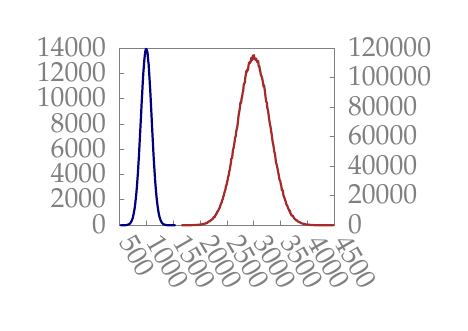
\begin{tikzpicture}[gnuplot, scale=0.3]
%% generated with GNUPLOT 5.2p2 (Lua 5.3; terminal rev. 99, script rev. 102)
%% wo 11 jul 2018 09:51:59 CEST
\path (0.000,0.000) rectangle (12.500,8.750);
\gpcolor{rgb color={0.502,0.502,0.502}}
\gpsetlinetype{gp lt border}
\gpsetdashtype{gp dt solid}
\gpsetlinewidth{1.00}
\draw[gp path] (1.380,0.945)--(1.560,0.945);
\node[gp node right] at (1.196,0.945) {$0$};
\draw[gp path] (1.380,2.016)--(1.560,2.016);
\node[gp node right] at (1.196,2.016) {$2000$};
\draw[gp path] (1.380,3.087)--(1.560,3.087);
\node[gp node right] at (1.196,3.087) {$4000$};
\draw[gp path] (1.380,4.158)--(1.560,4.158);
\node[gp node right] at (1.196,4.158) {$6000$};
\draw[gp path] (1.380,5.228)--(1.560,5.228);
\node[gp node right] at (1.196,5.228) {$8000$};
\draw[gp path] (1.380,6.299)--(1.560,6.299);
\node[gp node right] at (1.196,6.299) {$10000$};
\draw[gp path] (1.380,7.370)--(1.560,7.370);
\node[gp node right] at (1.196,7.370) {$12000$};
\draw[gp path] (1.380,8.441)--(1.560,8.441);
\node[gp node right] at (1.196,8.441) {$14000$};
\draw[gp path] (1.380,0.945)--(1.380,1.125);
\node[gp node left,rotate=-60] at (1.380,0.761) {$500$};
\draw[gp path] (2.517,0.945)--(2.517,1.125);
\node[gp node left,rotate=-60] at (2.517,0.761) {$1000$};
\draw[gp path] (3.654,0.945)--(3.654,1.125);
\node[gp node left,rotate=-60] at (3.654,0.761) {$1500$};
\draw[gp path] (4.791,0.945)--(4.791,1.125);
\node[gp node left,rotate=-60] at (4.791,0.761) {$2000$};
\draw[gp path] (5.928,0.945)--(5.928,1.125);
\node[gp node left,rotate=-60] at (5.928,0.761) {$2500$};
\draw[gp path] (7.064,0.945)--(7.064,1.125);
\node[gp node left,rotate=-60] at (7.064,0.761) {$3000$};
\draw[gp path] (8.201,0.945)--(8.201,1.125);
\node[gp node left,rotate=-60] at (8.201,0.761) {$3500$};
\draw[gp path] (9.338,0.945)--(9.338,1.125);
\node[gp node left,rotate=-60] at (9.338,0.761) {$4000$};
\draw[gp path] (10.475,0.945)--(10.475,1.125);
\node[gp node left,rotate=-60] at (10.475,0.761) {$4500$};
\draw[gp path] (10.475,0.945)--(10.295,0.945);
\node[gp node left] at (10.659,0.945) {$0$};
\draw[gp path] (10.475,2.194)--(10.295,2.194);
\node[gp node left] at (10.659,2.194) {$20000$};
\draw[gp path] (10.475,3.444)--(10.295,3.444);
\node[gp node left] at (10.659,3.444) {$40000$};
\draw[gp path] (10.475,4.693)--(10.295,4.693);
\node[gp node left] at (10.659,4.693) {$60000$};
\draw[gp path] (10.475,5.942)--(10.295,5.942);
\node[gp node left] at (10.659,5.942) {$80000$};
\draw[gp path] (10.475,7.192)--(10.295,7.192);
\node[gp node left] at (10.659,7.192) {$100000$};
\draw[gp path] (10.475,8.441)--(10.295,8.441);
\node[gp node left] at (10.659,8.441) {$120000$};
\draw[gp path] (1.380,8.441)--(1.380,0.945)--(10.475,0.945)--(10.475,8.441)--cycle;
\gpcolor{rgb color={0.647,0.165,0.165}}
\gpsetlinewidth{2.00}
\draw[gp path] (4.018,0.946)--(4.040,0.946)--(4.063,0.946)--(4.086,0.946)--(4.131,0.946)%
  --(4.154,0.946)--(4.177,0.946)--(4.199,0.946)--(4.222,0.947)--(4.245,0.946)--(4.268,0.947)%
  --(4.290,0.946)--(4.313,0.946)--(4.336,0.946)--(4.359,0.947)--(4.381,0.947)--(4.404,0.949)%
  --(4.427,0.948)--(4.450,0.949)--(4.472,0.951)--(4.495,0.950)--(4.518,0.952)--(4.541,0.951)%
  --(4.563,0.955)--(4.586,0.954)--(4.609,0.954)--(4.631,0.956)--(4.654,0.958)--(4.677,0.963)%
  --(4.700,0.961)--(4.722,0.959)--(4.745,0.965)--(4.768,0.969)--(4.791,0.978)--(4.813,0.975)%
  --(4.836,0.978)--(4.859,0.979)--(4.882,0.990)--(4.904,1.002)--(4.927,1.001)--(4.950,0.996)%
  --(4.973,1.012)--(4.995,1.019)--(5.018,1.016)--(5.041,1.032)--(5.063,1.060)--(5.086,1.042)%
  --(5.109,1.072)--(5.132,1.085)--(5.154,1.100)--(5.177,1.115)--(5.200,1.117)--(5.223,1.132)%
  --(5.245,1.165)--(5.268,1.172)--(5.291,1.195)--(5.314,1.205)--(5.336,1.242)--(5.359,1.276)%
  --(5.382,1.302)--(5.405,1.290)--(5.427,1.354)--(5.450,1.382)--(5.473,1.431)--(5.495,1.456)%
  --(5.518,1.528)--(5.541,1.543)--(5.564,1.586)--(5.586,1.646)--(5.609,1.674)--(5.632,1.742)%
  --(5.655,1.820)--(5.677,1.878)--(5.700,1.911)--(5.723,2.007)--(5.746,2.049)--(5.768,2.162)%
  --(5.791,2.206)--(5.814,2.318)--(5.837,2.398)--(5.859,2.460)--(5.882,2.627)--(5.905,2.633)%
  --(5.928,2.771)--(5.950,2.852)--(5.973,3.004)--(5.996,3.052)--(6.018,3.213)--(6.041,3.292)%
  --(6.064,3.446)--(6.087,3.565)--(6.109,3.775)--(6.132,3.777)--(6.155,3.912)--(6.178,4.155)%
  --(6.200,4.201)--(6.223,4.319)--(6.246,4.488)--(6.269,4.659)--(6.291,4.705)--(6.314,4.918)%
  --(6.337,5.012)--(6.360,5.115)--(6.382,5.279)--(6.405,5.512)--(6.428,5.678)--(6.450,5.785)%
  --(6.473,5.931)--(6.496,6.158)--(6.519,6.114)--(6.541,6.302)--(6.564,6.378)--(6.587,6.554)%
  --(6.610,6.631)--(6.632,6.881)--(6.655,6.949)--(6.678,6.981)--(6.701,7.204)--(6.723,7.344)%
  --(6.746,7.487)--(6.769,7.436)--(6.792,7.553)--(6.814,7.513)--(6.837,7.724)--(6.860,7.837)%
  --(6.882,7.793)--(6.905,7.877)--(6.928,7.859)--(6.951,8.028)--(6.973,7.986)--(6.996,7.934)%
  --(7.019,8.122)--(7.042,8.092)--(7.064,8.145)--(7.087,8.015)--(7.110,7.981)--(7.133,7.944)%
  --(7.155,8.000)--(7.178,7.926)--(7.201,7.857)--(7.224,7.851)--(7.246,7.890)--(7.269,7.657)%
  --(7.292,7.686)--(7.314,7.536)--(7.337,7.443)--(7.360,7.293)--(7.383,7.266)--(7.405,7.203)%
  --(7.428,7.094)--(7.451,6.958)--(7.474,6.810)--(7.496,6.870)--(7.519,6.692)--(7.542,6.497)%
  --(7.565,6.310)--(7.587,6.165)--(7.610,6.140)--(7.633,5.902)--(7.656,5.823)--(7.678,5.680)%
  --(7.701,5.495)--(7.724,5.336)--(7.747,5.204)--(7.769,5.096)--(7.792,4.926)--(7.815,4.804)%
  --(7.837,4.630)--(7.860,4.449)--(7.883,4.360)--(7.906,4.201)--(7.928,4.045)--(7.951,3.980)%
  --(7.974,3.807)--(7.997,3.597)--(8.019,3.543)--(8.042,3.452)--(8.065,3.329)--(8.088,3.212)%
  --(8.110,3.093)--(8.133,2.953)--(8.156,2.847)--(8.179,2.817)--(8.201,2.686)--(8.224,2.603)%
  --(8.247,2.430)--(8.269,2.439)--(8.292,2.391)--(8.315,2.198)--(8.338,2.156)--(8.360,2.083)%
  --(8.383,2.014)--(8.406,1.962)--(8.429,1.855)--(8.451,1.810)--(8.474,1.772)--(8.497,1.706)%
  --(8.520,1.651)--(8.542,1.604)--(8.565,1.548)--(8.588,1.559)--(8.611,1.443)--(8.633,1.419)%
  --(8.656,1.357)--(8.679,1.370)--(8.701,1.341)--(8.724,1.318)--(8.747,1.269)--(8.770,1.233)%
  --(8.792,1.216)--(8.815,1.193)--(8.838,1.168)--(8.861,1.139)--(8.883,1.154)--(8.906,1.120)%
  --(8.929,1.107)--(8.952,1.093)--(8.974,1.085)--(8.997,1.067)--(9.020,1.074)--(9.043,1.046)%
  --(9.065,1.030)--(9.088,1.023)--(9.111,1.024)--(9.133,1.001)--(9.156,1.015)--(9.179,1.004)%
  --(9.202,0.994)--(9.224,0.996)--(9.247,0.986)--(9.270,0.976)--(9.293,0.976)--(9.315,0.977)%
  --(9.338,0.976)--(9.361,0.965)--(9.384,0.964)--(9.406,0.962)--(9.429,0.963)--(9.452,0.959)%
  --(9.475,0.957)--(9.497,0.961)--(9.520,0.952)--(9.543,0.955)--(9.566,0.952)--(9.588,0.952)%
  --(9.611,0.951)--(9.634,0.948)--(9.656,0.948)--(9.679,0.949)--(9.702,0.949)--(9.725,0.950)%
  --(9.747,0.947)--(9.770,0.947)--(9.793,0.947)--(9.816,0.949)--(9.838,0.948)--(9.861,0.946)%
  --(9.884,0.946)--(9.907,0.947)--(9.975,0.946)--(9.998,0.946)--(10.043,0.946)--(10.066,0.946)%
  --(10.088,0.947)--(10.111,0.946)--(10.225,0.946)--(10.339,0.946)--(10.430,0.946);
\gpcolor{rgb color={0.000,0.000,0.502}}
\draw[gp path] (1.425,0.945)--(1.448,0.945)--(1.471,0.945)--(1.494,0.945)--(1.516,0.946)%
  --(1.539,0.946)--(1.562,0.947)--(1.585,0.947)--(1.607,0.947)--(1.630,0.949)--(1.653,0.951)%
  --(1.676,0.955)--(1.698,0.959)--(1.721,0.966)--(1.744,0.972)--(1.767,0.983)--(1.789,0.999)%
  --(1.812,1.014)--(1.835,1.041)--(1.857,1.074)--(1.880,1.118)--(1.903,1.164)--(1.926,1.227)%
  --(1.948,1.311)--(1.971,1.422)--(1.994,1.545)--(2.017,1.680)--(2.039,1.847)--(2.062,2.065)%
  --(2.085,2.279)--(2.108,2.541)--(2.130,2.844)--(2.153,3.166)--(2.176,3.544)--(2.199,3.930)%
  --(2.221,4.362)--(2.244,4.790)--(2.267,5.244)--(2.290,5.674)--(2.312,6.137)--(2.335,6.535)%
  --(2.358,6.999)--(2.380,7.360)--(2.403,7.666)--(2.426,7.959)--(2.449,8.169)--(2.471,8.328)%
  --(2.494,8.411)--(2.517,8.387)--(2.540,8.347)--(2.562,8.226)--(2.585,7.964)--(2.608,7.741)%
  --(2.631,7.368)--(2.653,7.004)--(2.676,6.639)--(2.699,6.189)--(2.722,5.736)--(2.744,5.287)%
  --(2.767,4.824)--(2.790,4.394)--(2.812,3.959)--(2.835,3.567)--(2.858,3.220)--(2.881,2.865)%
  --(2.903,2.573)--(2.926,2.308)--(2.949,2.059)--(2.972,1.872)--(2.994,1.697)--(3.017,1.548)%
  --(3.040,1.420)--(3.063,1.316)--(3.085,1.240)--(3.108,1.171)--(3.131,1.117)--(3.154,1.077)%
  --(3.176,1.040)--(3.199,1.021)--(3.222,0.997)--(3.244,0.984)--(3.267,0.974)--(3.290,0.962)%
  --(3.313,0.961)--(3.335,0.956)--(3.358,0.952)--(3.381,0.949)--(3.404,0.948)--(3.426,0.948)%
  --(3.449,0.946)--(3.472,0.946)--(3.495,0.946)--(3.517,0.945)--(3.540,0.945)--(3.563,0.945)%
  --(3.608,0.945)--(3.699,0.945)--(3.722,0.945);
%% coordinates of the plot area
\gpdefrectangularnode{gp plot 1}{\pgfpoint{1.380cm}{0.945cm}}{\pgfpoint{10.475cm}{8.441cm}}
\end{tikzpicture}
%% gnuplot variables

\end{tabular}
\end{center}
\caption{\label{fig:inputselection:normal_3to1_randomOn}
Same algorithm as in Figure~\ref{fig:inputselection:normal_1to1_randomOn}, but
now with 3:1 deposits:payments (i.e., many small deposits, fewer but larger
payments).
}
\end{figure}

\clearpage

\subsection{The \texttt{Random-Improve} algorithm}

We are now ready to present the coin selection algorithm we propose. The basic
idea is simple: we will randomly pick UTxO entries until we have reached
the required value, and then continue randomly picking UTxO entries to try and
reach a total value such that the the change value is roughly equal to the
payment.

This presents a dilemma though. Suppose we have already covered the minimum
value required, and we're trying to improve the change output. We pick an
output from the UTxO, and it turns out to be huge. What do we do? One option
is to discard it and continue searching, but this would result in coin selection
frequently traversing the entire UTxO, resulting in poor performance.

Fortunately, self organisation comes to the rescue again. We can set an upper
bound on the size of the change output we still consider acceptable (we will
set it to twice the payment value). Then we take advantage of the following
property.
%
\begin{quote}
\textbf{Self organisation principle 3.} Searching the UTxO for additional
entries to improve our change output is only useful if the UTxO contains entries
that are sufficiently small enough. But \emph{precisely when} the UTxO contains
many small entries, it is less likely that a randomly chosen UTxO entry will
push the total above the upper bound we set.
\end{quote}
%
In other words, our answer to ``what do we do when we happen to pick a huge UTxO
entry?'' is ``we stop trying to improve our selection''.
Figure~\ref{fig:RandomImprove} shows the full algorithm.

\begin{figure}[t]
\begin{enumerate}
\item Randomly select outputs from the UTxO until the payment value is covered. \\
(In the rare case that this fails because the maximum number of transaction
inputs has been exceeded, fall-back on the largest-first algorithm for this
step.)
\item Randomly select outputs from the UTxO, considering for each output if that
output is an \emph{improvement}. If it is, add it to the transaction, and keep
going. An output is considered an improvement when:
\begin{enumerate}
\item It doesn't exceed the specified upper limit
\item Adding the new output gets us closer to the ideal change value
\item It doesn't exceed the maximum number of transaction inputs.
\end{enumerate}
\end{enumerate}
\caption{\label{fig:RandomImprove}
  The \texttt{Random-Improve} algorithm. Side note for point (2a): we  use twice
  the value of the payment as the upper limit. Side note for point (2b): it
  might be that without the new output we are slightly below the ideal value,
  and with the new output we are slightly above; that is fine, as long as the
  absolute distance decreases.
}
\end{figure}

\subsection{Evaluation}

The algorithm (Figure~\ref{fig:RandomImprove}) is deceptively simple. Do the
self organisation principles we isolated really mean that order will emerge from
chaos? Simulations suggest, yes, it does. We already mentioned how random input
selection does a great job at cleaning up dust in
Figure~\ref{fig:inputselection:normal_3to1_largeThenRandom}; what we didn't
emphasise in that section is that the algorithm we simulated there is actually
our \texttt{Random-Improve} algorithm. Notice how the median change:payment
ratio is initially very low (indicative of a coin selection algorithm that is
generating a lot of dust outputs), but climbs rapidly back to 1 as soon as
\texttt{Random-Improve} kicks in. We already observed that it does indeed do an
excellent job at cleaning up the dust, quickly reducing the size of the UTxO.
The simulations in Figures~\ref{fig:inputselection:normal_1to1_randomOn}
and~\ref{fig:inputselection:normal_3to1_randomOn} are also the result of the
\texttt{Random-Improve} algorithm.

That said, of course the long term effects of a coin selection algorithm
can depend strongly on the nature of the distribution of deposits and payments.
It is therefore important that we evaluate the algorithm against a number
of different distributions.

\subsubsection{Normal distribution, 10:1 deposit:payment ratio}

We already evaluated `Random-Improve` against normally distributed payments and
deposits with a 1:1 ratio and a 3:1 ratio; perhaps more typical for exchange
nodes might be even higher ratios.
Figure~\ref{fig:inputselection:normal_10to1_randomOn} shows is a 10:1 ratio.

\begin{figure}[p]
\begin{center}
\scriptsize
\begin{tabular}{ll}
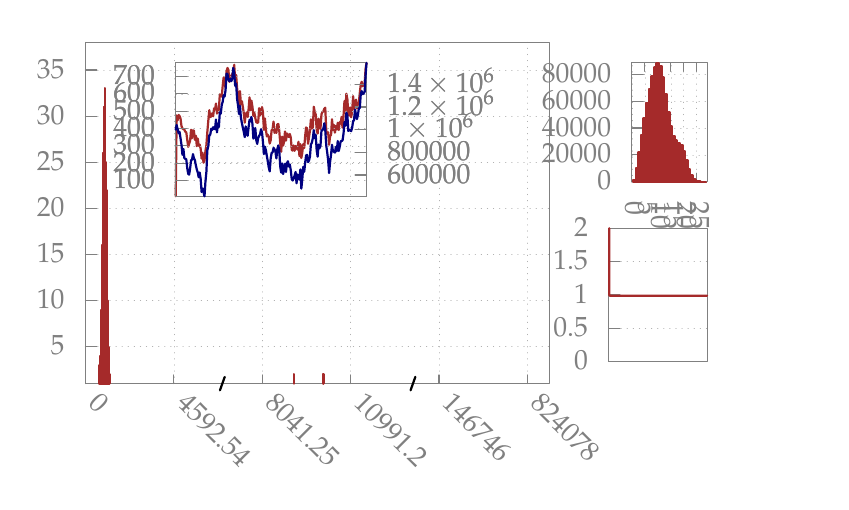
\begin{tikzpicture}[gnuplot, xscale=0.8, yscale=0.6]
%% generated with GNUPLOT 5.2p2 (Lua 5.3; terminal rev. 99, script rev. 102)
%% wo 11 jul 2018 11:09:08 CEST
\path (0.000,0.000) rectangle (12.500,8.750);
\gpcolor{color=gp lt color axes}
\gpsetlinetype{gp lt axes}
\gpsetdashtype{gp dt axes}
\gpsetlinewidth{0.50}
\draw[gp path] (0.828,1.999)--(8.197,1.999);
\gpcolor{rgb color={0.502,0.502,0.502}}
\gpsetlinetype{gp lt border}
\gpsetdashtype{gp dt solid}
\gpsetlinewidth{1.00}
\draw[gp path] (0.828,1.999)--(1.008,1.999);
\node[gp node right] at (0.644,1.999) {$5$};
\gpcolor{color=gp lt color axes}
\gpsetlinetype{gp lt axes}
\gpsetdashtype{gp dt axes}
\gpsetlinewidth{0.50}
\draw[gp path] (0.828,2.975)--(8.197,2.975);
\gpcolor{rgb color={0.502,0.502,0.502}}
\gpsetlinetype{gp lt border}
\gpsetdashtype{gp dt solid}
\gpsetlinewidth{1.00}
\draw[gp path] (0.828,2.975)--(1.008,2.975);
\node[gp node right] at (0.644,2.975) {$10$};
\gpcolor{color=gp lt color axes}
\gpsetlinetype{gp lt axes}
\gpsetdashtype{gp dt axes}
\gpsetlinewidth{0.50}
\draw[gp path] (0.828,3.951)--(8.197,3.951);
\gpcolor{rgb color={0.502,0.502,0.502}}
\gpsetlinetype{gp lt border}
\gpsetdashtype{gp dt solid}
\gpsetlinewidth{1.00}
\draw[gp path] (0.828,3.951)--(1.008,3.951);
\node[gp node right] at (0.644,3.951) {$15$};
\gpcolor{color=gp lt color axes}
\gpsetlinetype{gp lt axes}
\gpsetdashtype{gp dt axes}
\gpsetlinewidth{0.50}
\draw[gp path] (0.828,4.927)--(8.197,4.927);
\gpcolor{rgb color={0.502,0.502,0.502}}
\gpsetlinetype{gp lt border}
\gpsetdashtype{gp dt solid}
\gpsetlinewidth{1.00}
\draw[gp path] (0.828,4.927)--(1.008,4.927);
\node[gp node right] at (0.644,4.927) {$20$};
\gpcolor{color=gp lt color axes}
\gpsetlinetype{gp lt axes}
\gpsetdashtype{gp dt axes}
\gpsetlinewidth{0.50}
\draw[gp path] (0.828,5.903)--(8.197,5.903);
\gpcolor{rgb color={0.502,0.502,0.502}}
\gpsetlinetype{gp lt border}
\gpsetdashtype{gp dt solid}
\gpsetlinewidth{1.00}
\draw[gp path] (0.828,5.903)--(1.008,5.903);
\node[gp node right] at (0.644,5.903) {$25$};
\gpcolor{color=gp lt color axes}
\gpsetlinetype{gp lt axes}
\gpsetdashtype{gp dt axes}
\gpsetlinewidth{0.50}
\draw[gp path] (0.828,6.879)--(8.197,6.879);
\gpcolor{rgb color={0.502,0.502,0.502}}
\gpsetlinetype{gp lt border}
\gpsetdashtype{gp dt solid}
\gpsetlinewidth{1.00}
\draw[gp path] (0.828,6.879)--(1.008,6.879);
\node[gp node right] at (0.644,6.879) {$30$};
\gpcolor{color=gp lt color axes}
\gpsetlinetype{gp lt axes}
\gpsetdashtype{gp dt axes}
\gpsetlinewidth{0.50}
\draw[gp path] (0.828,7.855)--(8.197,7.855);
\gpcolor{rgb color={0.502,0.502,0.502}}
\gpsetlinetype{gp lt border}
\gpsetdashtype{gp dt solid}
\gpsetlinewidth{1.00}
\draw[gp path] (0.828,7.855)--(1.008,7.855);
\node[gp node right] at (0.644,7.855) {$35$};
\gpcolor{color=gp lt color axes}
\gpsetlinetype{gp lt axes}
\gpsetdashtype{gp dt axes}
\gpsetlinewidth{0.50}
\draw[gp path] (0.828,1.218)--(0.828,8.441);
\gpcolor{rgb color={0.502,0.502,0.502}}
\gpsetlinetype{gp lt border}
\gpsetdashtype{gp dt solid}
\gpsetlinewidth{1.00}
\draw[gp path] (0.828,1.218)--(0.828,1.398);
\node[gp node left,rotate=-45] at (0.828,1.034) {$0$};
\gpcolor{color=gp lt color axes}
\gpsetlinetype{gp lt axes}
\gpsetdashtype{gp dt axes}
\gpsetlinewidth{0.50}
\draw[gp path] (2.232,1.218)--(2.232,8.441);
\gpcolor{rgb color={0.502,0.502,0.502}}
\gpsetlinetype{gp lt border}
\gpsetdashtype{gp dt solid}
\gpsetlinewidth{1.00}
\draw[gp path] (2.232,1.218)--(2.232,1.398);
\node[gp node left,rotate=-45] at (2.232,1.034) {$4592.54$};
\gpcolor{color=gp lt color axes}
\gpsetlinetype{gp lt axes}
\gpsetdashtype{gp dt axes}
\gpsetlinewidth{0.50}
\draw[gp path] (3.635,1.218)--(3.635,8.441);
\gpcolor{rgb color={0.502,0.502,0.502}}
\gpsetlinetype{gp lt border}
\gpsetdashtype{gp dt solid}
\gpsetlinewidth{1.00}
\draw[gp path] (3.635,1.218)--(3.635,1.398);
\node[gp node left,rotate=-45] at (3.635,1.034) {$8041.25$};
\gpcolor{color=gp lt color axes}
\gpsetlinetype{gp lt axes}
\gpsetdashtype{gp dt axes}
\gpsetlinewidth{0.50}
\draw[gp path] (5.039,1.218)--(5.039,8.441);
\gpcolor{rgb color={0.502,0.502,0.502}}
\gpsetlinetype{gp lt border}
\gpsetdashtype{gp dt solid}
\gpsetlinewidth{1.00}
\draw[gp path] (5.039,1.218)--(5.039,1.398);
\node[gp node left,rotate=-45] at (5.039,1.034) {$10991.2$};
\gpcolor{color=gp lt color axes}
\gpsetlinetype{gp lt axes}
\gpsetdashtype{gp dt axes}
\gpsetlinewidth{0.50}
\draw[gp path] (6.442,1.218)--(6.442,8.441);
\gpcolor{rgb color={0.502,0.502,0.502}}
\gpsetlinetype{gp lt border}
\gpsetdashtype{gp dt solid}
\gpsetlinewidth{1.00}
\draw[gp path] (6.442,1.218)--(6.442,1.398);
\node[gp node left,rotate=-45] at (6.442,1.034) {$146746$};
\gpcolor{color=gp lt color axes}
\gpsetlinetype{gp lt axes}
\gpsetdashtype{gp dt axes}
\gpsetlinewidth{0.50}
\draw[gp path] (7.846,1.218)--(7.846,8.261)--(7.846,8.441);
\gpcolor{rgb color={0.502,0.502,0.502}}
\gpsetlinetype{gp lt border}
\gpsetdashtype{gp dt solid}
\gpsetlinewidth{1.00}
\draw[gp path] (7.846,1.218)--(7.846,1.398);
\node[gp node left,rotate=-45] at (7.846,1.034) {$824078$};
\draw[gp path] (0.828,8.441)--(0.828,1.218)--(8.197,1.218)--(8.197,8.441)--cycle;
\gpcolor{rgb color={0.647,0.165,0.165}}
\gpsetlinewidth{2.00}
\draw[gp path] (1.043,1.218)--(1.043,1.413)--(1.047,1.413)--(1.047,1.218)--cycle;
\draw[gp path] (1.053,1.218)--(1.053,1.608)--(1.056,1.608)--(1.056,1.218)--cycle;
\draw[gp path] (1.062,1.218)--(1.062,1.804)--(1.065,1.804)--(1.065,1.218)--cycle;
\draw[gp path] (1.065,1.218)--(1.065,1.608)--(1.068,1.608)--(1.068,1.218)--cycle;
\draw[gp path] (1.068,1.218)--(1.068,1.413)--(1.071,1.413)--(1.071,1.218)--cycle;
\draw[gp path] (1.071,1.218)--(1.071,1.608)--(1.074,1.608)--(1.074,1.218)--cycle;
\draw[gp path] (1.074,1.218)--(1.074,2.585)--(1.077,2.585)--(1.077,1.218)--cycle;
\draw[gp path] (1.077,1.218)--(1.077,1.999)--(1.080,1.999)--(1.080,1.218)--cycle;
\draw[gp path] (1.080,1.218)--(1.080,2.780)--(1.083,2.780)--(1.083,1.218)--cycle;
\draw[gp path] (1.083,1.218)--(1.083,1.999)--(1.086,1.999)--(1.086,1.218)--cycle;
\draw[gp path] (1.086,1.218)--(1.086,3.561)--(1.089,3.561)--(1.089,1.218)--cycle;
\draw[gp path] (1.089,1.218)--(1.089,3.365)--(1.092,3.365)--(1.092,1.218)--cycle;
\draw[gp path] (1.092,1.218)--(1.092,3.756)--(1.095,3.756)--(1.095,1.218)--cycle;
\draw[gp path] (1.095,1.218)--(1.095,4.146)--(1.098,4.146)--(1.098,1.218)--cycle;
\draw[gp path] (1.098,1.218)--(1.098,3.561)--(1.102,3.561)--(1.102,1.218)--cycle;
\draw[gp path] (1.102,1.218)--(1.102,4.537)--(1.105,4.537)--(1.105,1.218)--cycle;
\draw[gp path] (1.105,1.218)--(1.105,6.098)--(1.108,6.098)--(1.108,1.218)--cycle;
\draw[gp path] (1.108,1.218)--(1.108,5.318)--(1.111,5.318)--(1.111,1.218)--cycle;
\draw[gp path] (1.111,1.218)--(1.111,4.146)--(1.114,4.146)--(1.114,1.218)--cycle;
\draw[gp path] (1.114,1.218)--(1.114,4.146)--(1.117,4.146)--(1.117,1.218)--cycle;
\draw[gp path] (1.117,1.218)--(1.117,6.098)--(1.120,6.098)--(1.120,1.218)--cycle;
\draw[gp path] (1.120,1.218)--(1.120,7.074)--(1.123,7.074)--(1.123,1.218)--cycle;
\draw[gp path] (1.123,1.218)--(1.123,7.074)--(1.126,7.074)--(1.126,1.218)--cycle;
\draw[gp path] (1.126,1.218)--(1.126,5.903)--(1.129,5.903)--(1.129,1.218)--cycle;
\draw[gp path] (1.129,1.218)--(1.129,5.122)--(1.132,5.122)--(1.132,1.218)--cycle;
\draw[gp path] (1.132,1.218)--(1.132,5.903)--(1.135,5.903)--(1.135,1.218)--cycle;
\draw[gp path] (1.135,1.218)--(1.135,6.489)--(1.138,6.489)--(1.138,1.218)--cycle;
\draw[gp path] (1.138,1.218)--(1.138,6.879)--(1.141,6.879)--(1.141,1.218)--cycle;
\draw[gp path] (1.141,1.218)--(1.141,7.465)--(1.144,7.465)--(1.144,1.218)--cycle;
\draw[gp path] (1.144,1.218)--(1.144,4.732)--(1.147,4.732)--(1.147,1.218)--cycle;
\draw[gp path] (1.147,1.218)--(1.147,4.537)--(1.150,4.537)--(1.150,1.218)--cycle;
\draw[gp path] (1.150,1.218)--(1.150,5.708)--(1.153,5.708)--(1.153,1.218)--cycle;
\draw[gp path] (1.153,1.218)--(1.153,5.903)--(1.157,5.903)--(1.157,1.218)--cycle;
\draw[gp path] (1.157,1.218)--(1.157,5.318)--(1.160,5.318)--(1.160,1.218)--cycle;
\draw[gp path] (1.160,1.218)--(1.160,5.318)--(1.163,5.318)--(1.163,1.218)--cycle;
\draw[gp path] (1.163,1.218)--(1.163,4.732)--(1.166,4.732)--(1.166,1.218)--cycle;
\draw[gp path] (1.166,1.218)--(1.166,3.365)--(1.169,3.365)--(1.169,1.218)--cycle;
\draw[gp path] (1.169,1.218)--(1.169,2.585)--(1.172,2.585)--(1.172,1.218)--cycle;
\draw[gp path] (1.172,1.218)--(1.172,3.170)--(1.175,3.170)--(1.175,1.218)--cycle;
\draw[gp path] (1.175,1.218)--(1.175,2.975)--(1.178,2.975)--(1.178,1.218)--cycle;
\draw[gp path] (1.178,1.218)--(1.178,2.389)--(1.181,2.389)--(1.181,1.218)--cycle;
\draw[gp path] (1.181,1.218)--(1.181,1.608)--(1.184,1.608)--(1.184,1.218)--cycle;
\draw[gp path] (1.184,1.218)--(1.184,1.999)--(1.187,1.999)--(1.187,1.218)--cycle;
\draw[gp path] (1.187,1.218)--(1.187,1.608)--(1.190,1.608)--(1.190,1.218)--cycle;
\draw[gp path] (1.190,1.218)--(1.190,1.804)--(1.193,1.804)--(1.193,1.218)--cycle;
\draw[gp path] (1.193,1.218)--(1.193,1.804)--(1.196,1.804)--(1.196,1.218)--cycle;
\draw[gp path] (1.196,1.218)--(1.196,1.999)--(1.199,1.999)--(1.199,1.218)--cycle;
\draw[gp path] (1.199,1.218)--(1.199,1.413)--(1.202,1.413)--(1.202,1.218)--cycle;
\draw[gp path] (1.209,1.218)--(1.209,1.413)--(1.212,1.413)--(1.212,1.218)--cycle;
\draw[gp path] (4.137,1.218)--(4.137,1.413)--(4.141,1.413)--(4.141,1.218)--cycle;
\draw[gp path] (4.603,1.218)--(4.603,1.413)--(4.608,1.413)--(4.608,1.218)--cycle;
\gpcolor{color=gp lt color border}
\draw[gp path](2.964,1.074)--(3.040,1.358);
\draw[gp path](5.990,1.074)--(6.066,1.358);
%% coordinates of the plot area
\gpdefrectangularnode{gp plot 1}{\pgfpoint{0.828cm}{1.218cm}}{\pgfpoint{8.197cm}{8.441cm}}
\gpcolor{color=gp lt color axes}
\gpsetlinetype{gp lt axes}
\gpsetdashtype{gp dt axes}
\gpsetlinewidth{0.50}
\draw[gp path] (2.262,5.517)--(5.291,5.517);
\gpcolor{rgb color={0.502,0.502,0.502}}
\gpsetlinetype{gp lt border}
\gpsetdashtype{gp dt solid}
\gpsetlinewidth{1.00}
\draw[gp path] (2.262,5.517)--(2.442,5.517);
\node[gp node right] at (2.078,5.517) {$100$};
\gpcolor{color=gp lt color axes}
\gpsetlinetype{gp lt axes}
\gpsetdashtype{gp dt axes}
\gpsetlinewidth{0.50}
\draw[gp path] (2.262,5.883)--(5.291,5.883);
\gpcolor{rgb color={0.502,0.502,0.502}}
\gpsetlinetype{gp lt border}
\gpsetdashtype{gp dt solid}
\gpsetlinewidth{1.00}
\draw[gp path] (2.262,5.883)--(2.442,5.883);
\node[gp node right] at (2.078,5.883) {$200$};
\gpcolor{color=gp lt color axes}
\gpsetlinetype{gp lt axes}
\gpsetdashtype{gp dt axes}
\gpsetlinewidth{0.50}
\draw[gp path] (2.262,6.250)--(5.291,6.250);
\gpcolor{rgb color={0.502,0.502,0.502}}
\gpsetlinetype{gp lt border}
\gpsetdashtype{gp dt solid}
\gpsetlinewidth{1.00}
\draw[gp path] (2.262,6.250)--(2.442,6.250);
\node[gp node right] at (2.078,6.250) {$300$};
\gpcolor{color=gp lt color axes}
\gpsetlinetype{gp lt axes}
\gpsetdashtype{gp dt axes}
\gpsetlinewidth{0.50}
\draw[gp path] (2.262,6.616)--(5.291,6.616);
\gpcolor{rgb color={0.502,0.502,0.502}}
\gpsetlinetype{gp lt border}
\gpsetdashtype{gp dt solid}
\gpsetlinewidth{1.00}
\draw[gp path] (2.262,6.616)--(2.442,6.616);
\node[gp node right] at (2.078,6.616) {$400$};
\gpcolor{color=gp lt color axes}
\gpsetlinetype{gp lt axes}
\gpsetdashtype{gp dt axes}
\gpsetlinewidth{0.50}
\draw[gp path] (2.262,6.982)--(5.291,6.982);
\gpcolor{rgb color={0.502,0.502,0.502}}
\gpsetlinetype{gp lt border}
\gpsetdashtype{gp dt solid}
\gpsetlinewidth{1.00}
\draw[gp path] (2.262,6.982)--(2.442,6.982);
\node[gp node right] at (2.078,6.982) {$500$};
\gpcolor{color=gp lt color axes}
\gpsetlinetype{gp lt axes}
\gpsetdashtype{gp dt axes}
\gpsetlinewidth{0.50}
\draw[gp path] (2.262,7.348)--(5.291,7.348);
\gpcolor{rgb color={0.502,0.502,0.502}}
\gpsetlinetype{gp lt border}
\gpsetdashtype{gp dt solid}
\gpsetlinewidth{1.00}
\draw[gp path] (2.262,7.348)--(2.442,7.348);
\node[gp node right] at (2.078,7.348) {$600$};
\gpcolor{color=gp lt color axes}
\gpsetlinetype{gp lt axes}
\gpsetdashtype{gp dt axes}
\gpsetlinewidth{0.50}
\draw[gp path] (2.262,7.715)--(5.291,7.715);
\gpcolor{rgb color={0.502,0.502,0.502}}
\gpsetlinetype{gp lt border}
\gpsetdashtype{gp dt solid}
\gpsetlinewidth{1.00}
\draw[gp path] (2.262,7.715)--(2.442,7.715);
\node[gp node right] at (2.078,7.715) {$700$};
\draw[gp path] (5.291,5.631)--(5.111,5.631);
\node[gp node left] at (5.475,5.631) {$600000$};
\draw[gp path] (5.291,6.111)--(5.111,6.111);
\node[gp node left] at (5.475,6.111) {$800000$};
\draw[gp path] (5.291,6.591)--(5.111,6.591);
\node[gp node left] at (5.475,6.591) {$1\times10^{6}$};
\draw[gp path] (5.291,7.071)--(5.111,7.071);
\node[gp node left] at (5.475,7.071) {$1.2\times10^{6}$};
\draw[gp path] (5.291,7.550)--(5.111,7.550);
\node[gp node left] at (5.475,7.550) {$1.4\times10^{6}$};
\draw[gp path] (2.262,8.004)--(2.262,5.180)--(5.291,5.180)--(5.291,8.004)--cycle;
\gpcolor{rgb color={0.647,0.165,0.165}}
\gpsetlinewidth{2.00}
\draw[gp path] (2.262,5.180)--(2.277,6.894)--(2.292,6.788)--(2.308,6.902)--(2.323,6.880)%
  --(2.338,6.828)--(2.353,6.671)--(2.369,6.616)--(2.384,6.601)--(2.399,6.594)--(2.414,6.546)%
  --(2.429,6.539)--(2.445,6.381)--(2.460,6.228)--(2.475,6.293)--(2.490,6.356)--(2.506,6.590)%
  --(2.521,6.411)--(2.536,6.579)--(2.551,6.568)--(2.566,6.378)--(2.582,6.462)--(2.597,6.242)%
  --(2.612,6.403)--(2.627,6.250)--(2.643,6.272)--(2.658,6.187)--(2.673,5.978)--(2.688,6.099)%
  --(2.703,5.891)--(2.719,5.942)--(2.734,6.140)--(2.749,6.264)--(2.764,6.546)--(2.780,6.788)%
  --(2.795,7.004)--(2.810,6.858)--(2.825,6.872)--(2.840,6.938)--(2.856,6.876)--(2.871,7.041)%
  --(2.886,7.019)--(2.901,7.143)--(2.917,6.934)--(2.932,6.960)--(2.947,7.015)--(2.962,7.337)%
  --(2.977,7.319)--(2.993,7.290)--(3.008,7.524)--(3.023,7.696)--(3.038,7.623)--(3.053,7.469)%
  --(3.069,7.828)--(3.084,7.898)--(3.099,7.850)--(3.114,7.601)--(3.130,7.729)--(3.145,7.729)%
  --(3.160,7.770)--(3.175,7.795)--(3.190,7.964)--(3.206,7.649)--(3.221,7.748)--(3.236,7.477)%
  --(3.251,7.279)--(3.267,7.088)--(3.282,7.407)--(3.297,7.132)--(3.312,7.195)--(3.327,7.077)%
  --(3.343,6.938)--(3.358,6.740)--(3.373,6.912)--(3.388,6.956)--(3.404,6.861)--(3.419,7.030)%
  --(3.434,7.275)--(3.449,7.004)--(3.464,7.206)--(3.480,7.074)--(3.495,6.883)--(3.510,6.949)%
  --(3.525,6.839)--(3.541,6.748)--(3.556,6.737)--(3.571,6.744)--(3.586,7.048)--(3.601,6.891)%
  --(3.617,6.942)--(3.632,7.070)--(3.647,6.960)--(3.662,6.587)--(3.678,6.828)--(3.693,6.597)%
  --(3.708,6.451)--(3.723,6.484)--(3.738,6.440)--(3.754,6.297)--(3.769,6.363)--(3.784,6.576)%
  --(3.799,6.597)--(3.815,6.762)--(3.830,6.524)--(3.845,6.554)--(3.860,6.524)--(3.875,6.704)%
  --(3.891,6.711)--(3.906,6.565)--(3.921,6.304)--(3.936,6.125)--(3.952,6.444)--(3.967,6.253)%
  --(3.982,6.337)--(3.997,6.554)--(4.012,6.359)--(4.028,6.513)--(4.043,6.455)--(4.058,6.436)%
  --(4.073,6.499)--(4.089,6.425)--(4.104,6.165)--(4.119,6.147)--(4.134,6.257)--(4.149,6.143)%
  --(4.165,6.246)--(4.180,6.209)--(4.195,6.169)--(4.210,6.334)--(4.226,6.033)--(4.241,6.286)%
  --(4.256,5.993)--(4.271,6.103)--(4.286,6.286)--(4.302,6.202)--(4.317,6.458)--(4.332,6.638)%
  --(4.347,6.619)--(4.363,6.293)--(4.378,6.433)--(4.393,6.568)--(4.408,6.810)--(4.423,6.616)%
  --(4.439,6.641)--(4.454,7.077)--(4.469,6.964)--(4.484,6.916)--(4.500,6.583)--(4.515,6.510)%
  --(4.530,6.825)--(4.545,6.693)--(4.560,6.608)--(4.576,6.920)--(4.591,6.964)--(4.606,6.978)%
  --(4.621,7.033)--(4.636,7.055)--(4.652,6.568)--(4.667,6.499)--(4.682,6.535)--(4.697,6.272)%
  --(4.713,6.458)--(4.728,6.480)--(4.743,6.810)--(4.758,6.583)--(4.773,6.693)--(4.789,6.528)%
  --(4.804,6.667)--(4.819,6.597)--(4.834,6.737)--(4.850,6.583)--(4.865,6.748)--(4.880,6.722)%
  --(4.895,6.861)--(4.910,6.634)--(4.926,6.887)--(4.941,7.198)--(4.956,6.993)--(4.971,7.352)%
  --(4.987,7.235)--(5.002,6.927)--(5.017,6.891)--(5.032,7.063)--(5.047,6.854)--(5.063,6.975)%
  --(5.078,7.301)--(5.093,7.033)--(5.108,7.118)--(5.124,7.227)--(5.139,7.041)--(5.154,7.129)%
  --(5.169,7.165)--(5.184,7.367)--(5.200,7.550)--(5.215,7.605)--(5.230,7.510)--(5.245,7.539)%
  --(5.261,7.564)--(5.276,7.879)--(5.291,8.004);
%% coordinates of the plot area
\gpdefrectangularnode{gp plot 2}{\pgfpoint{2.262cm}{5.180cm}}{\pgfpoint{5.291cm}{8.004cm}}
\gpcolor{color=gp lt color axes}
\gpsetlinetype{gp lt axes}
\gpsetdashtype{gp dt axes}
\gpsetlinewidth{0.50}
\draw[gp path] (2.262,5.517)--(5.291,5.517);
\gpcolor{rgb color={0.502,0.502,0.502}}
\gpsetlinetype{gp lt border}
\gpsetdashtype{gp dt solid}
\gpsetlinewidth{1.00}
\draw[gp path] (2.262,5.517)--(2.442,5.517);
\node[gp node right] at (2.078,5.517) {$100$};
\gpcolor{color=gp lt color axes}
\gpsetlinetype{gp lt axes}
\gpsetdashtype{gp dt axes}
\gpsetlinewidth{0.50}
\draw[gp path] (2.262,5.883)--(5.291,5.883);
\gpcolor{rgb color={0.502,0.502,0.502}}
\gpsetlinetype{gp lt border}
\gpsetdashtype{gp dt solid}
\gpsetlinewidth{1.00}
\draw[gp path] (2.262,5.883)--(2.442,5.883);
\node[gp node right] at (2.078,5.883) {$200$};
\gpcolor{color=gp lt color axes}
\gpsetlinetype{gp lt axes}
\gpsetdashtype{gp dt axes}
\gpsetlinewidth{0.50}
\draw[gp path] (2.262,6.250)--(5.291,6.250);
\gpcolor{rgb color={0.502,0.502,0.502}}
\gpsetlinetype{gp lt border}
\gpsetdashtype{gp dt solid}
\gpsetlinewidth{1.00}
\draw[gp path] (2.262,6.250)--(2.442,6.250);
\node[gp node right] at (2.078,6.250) {$300$};
\gpcolor{color=gp lt color axes}
\gpsetlinetype{gp lt axes}
\gpsetdashtype{gp dt axes}
\gpsetlinewidth{0.50}
\draw[gp path] (2.262,6.616)--(5.291,6.616);
\gpcolor{rgb color={0.502,0.502,0.502}}
\gpsetlinetype{gp lt border}
\gpsetdashtype{gp dt solid}
\gpsetlinewidth{1.00}
\draw[gp path] (2.262,6.616)--(2.442,6.616);
\node[gp node right] at (2.078,6.616) {$400$};
\gpcolor{color=gp lt color axes}
\gpsetlinetype{gp lt axes}
\gpsetdashtype{gp dt axes}
\gpsetlinewidth{0.50}
\draw[gp path] (2.262,6.982)--(5.291,6.982);
\gpcolor{rgb color={0.502,0.502,0.502}}
\gpsetlinetype{gp lt border}
\gpsetdashtype{gp dt solid}
\gpsetlinewidth{1.00}
\draw[gp path] (2.262,6.982)--(2.442,6.982);
\node[gp node right] at (2.078,6.982) {$500$};
\gpcolor{color=gp lt color axes}
\gpsetlinetype{gp lt axes}
\gpsetdashtype{gp dt axes}
\gpsetlinewidth{0.50}
\draw[gp path] (2.262,7.348)--(5.291,7.348);
\gpcolor{rgb color={0.502,0.502,0.502}}
\gpsetlinetype{gp lt border}
\gpsetdashtype{gp dt solid}
\gpsetlinewidth{1.00}
\draw[gp path] (2.262,7.348)--(2.442,7.348);
\node[gp node right] at (2.078,7.348) {$600$};
\gpcolor{color=gp lt color axes}
\gpsetlinetype{gp lt axes}
\gpsetdashtype{gp dt axes}
\gpsetlinewidth{0.50}
\draw[gp path] (2.262,7.715)--(5.291,7.715);
\gpcolor{rgb color={0.502,0.502,0.502}}
\gpsetlinetype{gp lt border}
\gpsetdashtype{gp dt solid}
\gpsetlinewidth{1.00}
\draw[gp path] (2.262,7.715)--(2.442,7.715);
\node[gp node right] at (2.078,7.715) {$700$};
\draw[gp path] (5.291,5.631)--(5.111,5.631);
\node[gp node left] at (5.475,5.631) {$600000$};
\draw[gp path] (5.291,6.111)--(5.111,6.111);
\node[gp node left] at (5.475,6.111) {$800000$};
\draw[gp path] (5.291,6.591)--(5.111,6.591);
\node[gp node left] at (5.475,6.591) {$1\times10^{6}$};
\draw[gp path] (5.291,7.071)--(5.111,7.071);
\node[gp node left] at (5.475,7.071) {$1.2\times10^{6}$};
\draw[gp path] (5.291,7.550)--(5.111,7.550);
\node[gp node left] at (5.475,7.550) {$1.4\times10^{6}$};
\draw[gp path] (2.262,8.004)--(2.262,5.180)--(5.291,5.180)--(5.291,8.004)--cycle;
\gpcolor{rgb color={0.000,0.000,0.502}}
\gpsetlinewidth{2.00}
\draw[gp path] (2.262,6.592)--(2.277,6.690)--(2.292,6.600)--(2.308,6.516)--(2.323,6.545)%
  --(2.338,6.413)--(2.353,6.276)--(2.369,6.059)--(2.384,6.182)--(2.399,5.993)--(2.414,5.973)%
  --(2.429,5.968)--(2.445,5.780)--(2.460,5.657)--(2.475,5.639)--(2.490,5.766)--(2.506,5.946)%
  --(2.521,5.954)--(2.536,6.073)--(2.551,5.986)--(2.566,5.949)--(2.582,5.833)--(2.597,5.748)%
  --(2.612,5.688)--(2.627,5.584)--(2.643,5.685)--(2.658,5.549)--(2.673,5.272)--(2.688,5.346)%
  --(2.703,5.270)--(2.719,5.180)--(2.734,5.496)--(2.749,5.697)--(2.764,6.158)--(2.780,6.246)%
  --(2.795,6.473)--(2.810,6.483)--(2.825,6.610)--(2.840,6.584)--(2.856,6.643)--(2.871,6.611)%
  --(2.886,6.603)--(2.901,6.807)--(2.917,6.534)--(2.932,6.717)--(2.947,6.648)--(2.962,6.955)%
  --(2.977,6.930)--(2.993,7.118)--(3.008,7.184)--(3.023,7.320)--(3.038,7.291)--(3.053,7.427)%
  --(3.069,7.778)--(3.084,7.766)--(3.099,7.649)--(3.114,7.618)--(3.130,7.664)--(3.145,7.618)%
  --(3.160,7.672)--(3.175,7.898)--(3.190,7.791)--(3.206,7.517)--(3.221,7.563)--(3.236,7.243)%
  --(3.251,7.109)--(3.267,6.921)--(3.282,7.096)--(3.297,6.843)--(3.312,6.735)--(3.327,6.638)%
  --(3.343,6.540)--(3.358,6.434)--(3.373,6.660)--(3.388,6.500)--(3.404,6.462)--(3.419,6.646)%
  --(3.434,6.800)--(3.449,6.771)--(3.464,6.860)--(3.480,6.711)--(3.495,6.402)--(3.510,6.426)%
  --(3.525,6.625)--(3.541,6.369)--(3.556,6.290)--(3.571,6.413)--(3.586,6.460)--(3.601,6.494)%
  --(3.617,6.599)--(3.632,6.531)--(3.647,6.329)--(3.662,6.074)--(3.678,6.231)--(3.693,6.158)%
  --(3.708,6.040)--(3.723,5.927)--(3.738,5.801)--(3.754,5.708)--(3.769,5.974)--(3.784,6.098)%
  --(3.799,6.108)--(3.815,6.204)--(3.830,6.177)--(3.845,6.125)--(3.860,5.983)--(3.875,6.178)%
  --(3.891,6.259)--(3.906,6.153)--(3.921,5.810)--(3.936,5.684)--(3.952,5.876)--(3.967,5.652)%
  --(3.982,5.759)--(3.997,5.869)--(4.012,5.696)--(4.028,5.885)--(4.043,5.923)--(4.058,5.811)%
  --(4.073,5.853)--(4.089,5.727)--(4.104,5.541)--(4.119,5.516)--(4.134,5.552)--(4.149,5.620)%
  --(4.165,5.695)--(4.180,5.455)--(4.195,5.642)--(4.210,5.605)--(4.226,5.534)--(4.241,5.749)%
  --(4.256,5.344)--(4.271,5.538)--(4.286,5.803)--(4.302,5.700)--(4.317,5.893)--(4.332,6.048)%
  --(4.347,6.057)--(4.363,5.904)--(4.378,5.938)--(4.393,6.023)--(4.408,6.279)--(4.423,6.313)%
  --(4.439,6.412)--(4.454,6.582)--(4.469,6.411)--(4.484,6.481)--(4.500,6.153)--(4.515,6.019)%
  --(4.530,6.275)--(4.545,6.197)--(4.560,6.246)--(4.576,6.574)--(4.591,6.580)--(4.606,6.613)%
  --(4.621,6.727)--(4.636,6.586)--(4.652,6.250)--(4.667,6.110)--(4.682,5.938)--(4.697,5.674)%
  --(4.713,5.911)--(4.728,6.064)--(4.743,6.271)--(4.758,6.133)--(4.773,6.127)--(4.789,6.106)%
  --(4.804,6.224)--(4.819,6.135)--(4.834,6.350)--(4.850,6.140)--(4.865,6.227)--(4.880,6.341)%
  --(4.895,6.355)--(4.910,6.359)--(4.926,6.511)--(4.941,6.750)--(4.956,6.676)--(4.971,6.951)%
  --(4.987,6.895)--(5.002,6.563)--(5.017,6.580)--(5.032,6.586)--(5.047,6.559)--(5.063,6.634)%
  --(5.078,6.773)--(5.093,6.790)--(5.108,7.018)--(5.124,6.912)--(5.139,6.816)--(5.154,6.896)%
  --(5.169,7.044)--(5.184,7.047)--(5.200,7.354)--(5.215,7.406)--(5.230,7.344)--(5.245,7.358)%
  --(5.261,7.390)--(5.276,7.742)--(5.291,8.004);
\gpcolor{color=gp lt color axes}
\gpsetlinetype{gp lt axes}
\gpsetdashtype{gp dt axes}
\gpsetlinewidth{0.50}
\draw[gp path] (9.504,5.488)--(10.697,5.488);
\gpcolor{rgb color={0.502,0.502,0.502}}
\gpsetlinetype{gp lt border}
\gpsetdashtype{gp dt solid}
\gpsetlinewidth{1.00}
\draw[gp path] (9.504,5.488)--(9.684,5.488);
\node[gp node right] at (9.320,5.488) {$0$};
\gpcolor{color=gp lt color axes}
\gpsetlinetype{gp lt axes}
\gpsetdashtype{gp dt axes}
\gpsetlinewidth{0.50}
\draw[gp path] (9.504,6.057)--(10.697,6.057);
\gpcolor{rgb color={0.502,0.502,0.502}}
\gpsetlinetype{gp lt border}
\gpsetdashtype{gp dt solid}
\gpsetlinewidth{1.00}
\draw[gp path] (9.504,6.057)--(9.684,6.057);
\node[gp node right] at (9.320,6.057) {$20000$};
\gpcolor{color=gp lt color axes}
\gpsetlinetype{gp lt axes}
\gpsetdashtype{gp dt axes}
\gpsetlinewidth{0.50}
\draw[gp path] (9.504,6.626)--(10.697,6.626);
\gpcolor{rgb color={0.502,0.502,0.502}}
\gpsetlinetype{gp lt border}
\gpsetdashtype{gp dt solid}
\gpsetlinewidth{1.00}
\draw[gp path] (9.504,6.626)--(9.684,6.626);
\node[gp node right] at (9.320,6.626) {$40000$};
\gpcolor{color=gp lt color axes}
\gpsetlinetype{gp lt axes}
\gpsetdashtype{gp dt axes}
\gpsetlinewidth{0.50}
\draw[gp path] (9.504,7.195)--(10.697,7.195);
\gpcolor{rgb color={0.502,0.502,0.502}}
\gpsetlinetype{gp lt border}
\gpsetdashtype{gp dt solid}
\gpsetlinewidth{1.00}
\draw[gp path] (9.504,7.195)--(9.684,7.195);
\node[gp node right] at (9.320,7.195) {$60000$};
\gpcolor{color=gp lt color axes}
\gpsetlinetype{gp lt axes}
\gpsetdashtype{gp dt axes}
\gpsetlinewidth{0.50}
\draw[gp path] (9.504,7.764)--(10.697,7.764);
\gpcolor{rgb color={0.502,0.502,0.502}}
\gpsetlinetype{gp lt border}
\gpsetdashtype{gp dt solid}
\gpsetlinewidth{1.00}
\draw[gp path] (9.504,7.764)--(9.684,7.764);
\node[gp node right] at (9.320,7.764) {$80000$};
\gpcolor{color=gp lt color axes}
\gpsetlinetype{gp lt axes}
\gpsetdashtype{gp dt axes}
\gpsetlinewidth{0.50}
\draw[gp path] (9.504,5.488)--(9.504,7.824)--(9.504,8.004);
\gpcolor{rgb color={0.502,0.502,0.502}}
\gpsetlinetype{gp lt border}
\gpsetdashtype{gp dt solid}
\gpsetlinewidth{1.00}
\draw[gp path] (9.504,5.488)--(9.504,5.668);
\draw[gp path] (9.504,8.004)--(9.504,7.824);
\node[gp node left,rotate=-90] at (9.504,5.304) {$0$};
\gpcolor{color=gp lt color axes}
\gpsetlinetype{gp lt axes}
\gpsetdashtype{gp dt axes}
\gpsetlinewidth{0.50}
\draw[gp path] (9.710,5.488)--(9.710,7.824)--(9.710,8.004);
\gpcolor{rgb color={0.502,0.502,0.502}}
\gpsetlinetype{gp lt border}
\gpsetdashtype{gp dt solid}
\gpsetlinewidth{1.00}
\draw[gp path] (9.710,5.488)--(9.710,5.668);
\draw[gp path] (9.710,8.004)--(9.710,7.824);
\node[gp node left,rotate=-90] at (9.710,5.304) {$5$};
\gpcolor{color=gp lt color axes}
\gpsetlinetype{gp lt axes}
\gpsetdashtype{gp dt axes}
\gpsetlinewidth{0.50}
\draw[gp path] (9.915,5.488)--(9.915,7.824)--(9.915,8.004);
\gpcolor{rgb color={0.502,0.502,0.502}}
\gpsetlinetype{gp lt border}
\gpsetdashtype{gp dt solid}
\gpsetlinewidth{1.00}
\draw[gp path] (9.915,5.488)--(9.915,5.668);
\draw[gp path] (9.915,8.004)--(9.915,7.824);
\node[gp node left,rotate=-90] at (9.915,5.304) {$10$};
\gpcolor{color=gp lt color axes}
\gpsetlinetype{gp lt axes}
\gpsetdashtype{gp dt axes}
\gpsetlinewidth{0.50}
\draw[gp path] (10.121,5.488)--(10.121,7.824)--(10.121,8.004);
\gpcolor{rgb color={0.502,0.502,0.502}}
\gpsetlinetype{gp lt border}
\gpsetdashtype{gp dt solid}
\gpsetlinewidth{1.00}
\draw[gp path] (10.121,5.488)--(10.121,5.668);
\draw[gp path] (10.121,8.004)--(10.121,7.824);
\node[gp node left,rotate=-90] at (10.121,5.304) {$15$};
\gpcolor{color=gp lt color axes}
\gpsetlinetype{gp lt axes}
\gpsetdashtype{gp dt axes}
\gpsetlinewidth{0.50}
\draw[gp path] (10.327,5.488)--(10.327,7.824)--(10.327,8.004);
\gpcolor{rgb color={0.502,0.502,0.502}}
\gpsetlinetype{gp lt border}
\gpsetdashtype{gp dt solid}
\gpsetlinewidth{1.00}
\draw[gp path] (10.327,5.488)--(10.327,5.668);
\draw[gp path] (10.327,8.004)--(10.327,7.824);
\node[gp node left,rotate=-90] at (10.327,5.304) {$20$};
\gpcolor{color=gp lt color axes}
\gpsetlinetype{gp lt axes}
\gpsetdashtype{gp dt axes}
\gpsetlinewidth{0.50}
\draw[gp path] (10.532,5.488)--(10.532,8.004);
\gpcolor{rgb color={0.502,0.502,0.502}}
\gpsetlinetype{gp lt border}
\gpsetdashtype{gp dt solid}
\gpsetlinewidth{1.00}
\draw[gp path] (10.532,5.488)--(10.532,5.668);
\draw[gp path] (10.532,8.004)--(10.532,7.824);
\node[gp node left,rotate=-90] at (10.532,5.304) {$25$};
\draw[gp path] (9.504,8.004)--(9.504,5.488)--(10.697,5.488)--(10.697,8.004)--cycle;
\gpfill{rgb color={0.647,0.165,0.165}} (9.525,5.488)--(9.567,5.488)--(9.567,5.528)--(9.525,5.528)--cycle;
\gpcolor{rgb color={0.647,0.165,0.165}}
\gpsetlinewidth{2.00}
\draw[gp path] (9.525,5.488)--(9.525,5.527)--(9.566,5.527)--(9.566,5.488)--cycle;
\gpfill{rgb color={0.647,0.165,0.165}} (9.566,5.488)--(9.608,5.488)--(9.608,5.784)--(9.566,5.784)--cycle;
\draw[gp path] (9.566,5.488)--(9.566,5.783)--(9.607,5.783)--(9.607,5.488)--cycle;
\gpfill{rgb color={0.647,0.165,0.165}} (9.607,5.488)--(9.649,5.488)--(9.649,6.121)--(9.607,6.121)--cycle;
\draw[gp path] (9.607,5.488)--(9.607,6.120)--(9.648,6.120)--(9.648,5.488)--cycle;
\gpfill{rgb color={0.647,0.165,0.165}} (9.648,5.488)--(9.690,5.488)--(9.690,6.472)--(9.648,6.472)--cycle;
\draw[gp path] (9.648,5.488)--(9.648,6.471)--(9.689,6.471)--(9.689,5.488)--cycle;
\gpfill{rgb color={0.647,0.165,0.165}} (9.689,5.488)--(9.731,5.488)--(9.731,6.837)--(9.689,6.837)--cycle;
\draw[gp path] (9.689,5.488)--(9.689,6.836)--(9.730,6.836)--(9.730,5.488)--cycle;
\gpfill{rgb color={0.647,0.165,0.165}} (9.730,5.488)--(9.772,5.488)--(9.772,7.160)--(9.730,7.160)--cycle;
\draw[gp path] (9.730,5.488)--(9.730,7.159)--(9.771,7.159)--(9.771,5.488)--cycle;
\gpfill{rgb color={0.647,0.165,0.165}} (9.771,5.488)--(9.814,5.488)--(9.814,7.445)--(9.771,7.445)--cycle;
\draw[gp path] (9.771,5.488)--(9.771,7.444)--(9.813,7.444)--(9.813,5.488)--cycle;
\gpfill{rgb color={0.647,0.165,0.165}} (9.813,5.488)--(9.855,5.488)--(9.855,7.717)--(9.813,7.717)--cycle;
\draw[gp path] (9.813,5.488)--(9.813,7.716)--(9.854,7.716)--(9.854,5.488)--cycle;
\gpfill{rgb color={0.647,0.165,0.165}} (9.854,5.488)--(9.896,5.488)--(9.896,7.907)--(9.854,7.907)--cycle;
\draw[gp path] (9.854,5.488)--(9.854,7.906)--(9.895,7.906)--(9.895,5.488)--cycle;
\gpfill{rgb color={0.647,0.165,0.165}} (9.895,5.488)--(9.937,5.488)--(9.937,8.005)--(9.895,8.005)--cycle;
\draw[gp path] (9.895,5.488)--(9.895,8.004)--(9.936,8.004)--(9.936,5.488)--cycle;
\gpfill{rgb color={0.647,0.165,0.165}} (9.936,5.488)--(9.978,5.488)--(9.978,7.936)--(9.936,7.936)--cycle;
\draw[gp path] (9.936,5.488)--(9.936,7.935)--(9.977,7.935)--(9.977,5.488)--cycle;
\gpfill{rgb color={0.647,0.165,0.165}} (9.977,5.488)--(10.019,5.488)--(10.019,7.698)--(9.977,7.698)--cycle;
\draw[gp path] (9.977,5.488)--(9.977,7.697)--(10.018,7.697)--(10.018,5.488)--cycle;
\gpfill{rgb color={0.647,0.165,0.165}} (10.018,5.488)--(10.060,5.488)--(10.060,7.341)--(10.018,7.341)--cycle;
\draw[gp path] (10.018,5.488)--(10.018,7.340)--(10.059,7.340)--(10.059,5.488)--cycle;
\gpfill{rgb color={0.647,0.165,0.165}} (10.059,5.488)--(10.102,5.488)--(10.102,6.972)--(10.059,6.972)--cycle;
\draw[gp path] (10.059,5.488)--(10.059,6.971)--(10.101,6.971)--(10.101,5.488)--cycle;
\gpfill{rgb color={0.647,0.165,0.165}} (10.101,5.488)--(10.143,5.488)--(10.143,6.673)--(10.101,6.673)--cycle;
\draw[gp path] (10.101,5.488)--(10.101,6.672)--(10.142,6.672)--(10.142,5.488)--cycle;
\gpfill{rgb color={0.647,0.165,0.165}} (10.142,5.488)--(10.184,5.488)--(10.184,6.463)--(10.142,6.463)--cycle;
\draw[gp path] (10.142,5.488)--(10.142,6.462)--(10.183,6.462)--(10.183,5.488)--cycle;
\gpfill{rgb color={0.647,0.165,0.165}} (10.183,5.488)--(10.225,5.488)--(10.225,6.363)--(10.183,6.363)--cycle;
\draw[gp path] (10.183,5.488)--(10.183,6.362)--(10.224,6.362)--(10.224,5.488)--cycle;
\gpfill{rgb color={0.647,0.165,0.165}} (10.224,5.488)--(10.266,5.488)--(10.266,6.312)--(10.224,6.312)--cycle;
\draw[gp path] (10.224,5.488)--(10.224,6.311)--(10.265,6.311)--(10.265,5.488)--cycle;
\gpfill{rgb color={0.647,0.165,0.165}} (10.265,5.488)--(10.307,5.488)--(10.307,6.262)--(10.265,6.262)--cycle;
\draw[gp path] (10.265,5.488)--(10.265,6.261)--(10.306,6.261)--(10.306,5.488)--cycle;
\gpfill{rgb color={0.647,0.165,0.165}} (10.306,5.488)--(10.348,5.488)--(10.348,6.142)--(10.306,6.142)--cycle;
\draw[gp path] (10.306,5.488)--(10.306,6.141)--(10.347,6.141)--(10.347,5.488)--cycle;
\gpfill{rgb color={0.647,0.165,0.165}} (10.347,5.488)--(10.389,5.488)--(10.389,5.955)--(10.347,5.955)--cycle;
\draw[gp path] (10.347,5.488)--(10.347,5.954)--(10.388,5.954)--(10.388,5.488)--cycle;
\gpfill{rgb color={0.647,0.165,0.165}} (10.388,5.488)--(10.431,5.488)--(10.431,5.765)--(10.388,5.765)--cycle;
\draw[gp path] (10.388,5.488)--(10.388,5.764)--(10.430,5.764)--(10.430,5.488)--cycle;
\gpfill{rgb color={0.647,0.165,0.165}} (10.430,5.488)--(10.472,5.488)--(10.472,5.623)--(10.430,5.623)--cycle;
\draw[gp path] (10.430,5.488)--(10.430,5.622)--(10.471,5.622)--(10.471,5.488)--cycle;
\gpfill{rgb color={0.647,0.165,0.165}} (10.471,5.488)--(10.513,5.488)--(10.513,5.538)--(10.471,5.538)--cycle;
\draw[gp path] (10.471,5.488)--(10.471,5.537)--(10.512,5.537)--(10.512,5.488)--cycle;
\gpfill{rgb color={0.647,0.165,0.165}} (10.512,5.488)--(10.554,5.488)--(10.554,5.504)--(10.512,5.504)--cycle;
\draw[gp path] (10.512,5.488)--(10.512,5.503)--(10.553,5.503)--(10.553,5.488)--cycle;
\gpfill{rgb color={0.647,0.165,0.165}} (10.553,5.488)--(10.595,5.488)--(10.595,5.493)--(10.553,5.493)--cycle;
\draw[gp path] (10.553,5.488)--(10.553,5.492)--(10.594,5.492)--(10.594,5.488)--cycle;
\gpfill{rgb color={0.647,0.165,0.165}} (10.594,5.488)--(10.636,5.488)--(10.636,5.490)--(10.594,5.490)--cycle;
\draw[gp path] (10.594,5.488)--(10.594,5.489)--(10.635,5.489)--(10.635,5.488)--cycle;
\gpfill{rgb color={0.647,0.165,0.165}} (10.635,5.488)--(10.677,5.488)--(10.677,5.489)--(10.635,5.489)--cycle;
\draw[gp path] (10.635,5.488)--(10.676,5.488)--cycle;
%% coordinates of the plot area
\gpdefrectangularnode{gp plot 3}{\pgfpoint{9.504cm}{5.488cm}}{\pgfpoint{10.697cm}{8.004cm}}
\gpcolor{color=gp lt color axes}
\gpsetlinetype{gp lt axes}
\gpsetdashtype{gp dt axes}
\gpsetlinewidth{0.50}
\draw[gp path] (9.136,1.680)--(10.697,1.680);
\gpcolor{rgb color={0.502,0.502,0.502}}
\gpsetlinetype{gp lt border}
\gpsetdashtype{gp dt solid}
\gpsetlinewidth{1.00}
\draw[gp path] (9.136,1.680)--(9.316,1.680);
\node[gp node right] at (8.952,1.680) {$0$};
\gpcolor{color=gp lt color axes}
\gpsetlinetype{gp lt axes}
\gpsetdashtype{gp dt axes}
\gpsetlinewidth{0.50}
\draw[gp path] (9.136,2.386)--(10.697,2.386);
\gpcolor{rgb color={0.502,0.502,0.502}}
\gpsetlinetype{gp lt border}
\gpsetdashtype{gp dt solid}
\gpsetlinewidth{1.00}
\draw[gp path] (9.136,2.386)--(9.316,2.386);
\node[gp node right] at (8.952,2.386) {$0.5$};
\gpcolor{color=gp lt color axes}
\gpsetlinetype{gp lt axes}
\gpsetdashtype{gp dt axes}
\gpsetlinewidth{0.50}
\draw[gp path] (9.136,3.092)--(10.697,3.092);
\gpcolor{rgb color={0.502,0.502,0.502}}
\gpsetlinetype{gp lt border}
\gpsetdashtype{gp dt solid}
\gpsetlinewidth{1.00}
\draw[gp path] (9.136,3.092)--(9.316,3.092);
\node[gp node right] at (8.952,3.092) {$1$};
\gpcolor{color=gp lt color axes}
\gpsetlinetype{gp lt axes}
\gpsetdashtype{gp dt axes}
\gpsetlinewidth{0.50}
\draw[gp path] (9.136,3.798)--(10.697,3.798);
\gpcolor{rgb color={0.502,0.502,0.502}}
\gpsetlinetype{gp lt border}
\gpsetdashtype{gp dt solid}
\gpsetlinewidth{1.00}
\draw[gp path] (9.136,3.798)--(9.316,3.798);
\node[gp node right] at (8.952,3.798) {$1.5$};
\gpcolor{color=gp lt color axes}
\gpsetlinetype{gp lt axes}
\gpsetdashtype{gp dt axes}
\gpsetlinewidth{0.50}
\draw[gp path] (9.136,4.504)--(10.697,4.504);
\gpcolor{rgb color={0.502,0.502,0.502}}
\gpsetlinetype{gp lt border}
\gpsetdashtype{gp dt solid}
\gpsetlinewidth{1.00}
\draw[gp path] (9.136,4.504)--(9.316,4.504);
\node[gp node right] at (8.952,4.504) {$2$};
\draw[gp path] (9.136,4.504)--(9.136,1.680)--(10.697,1.680)--(10.697,4.504)--cycle;
\gpcolor{rgb color={0.647,0.165,0.165}}
\gpsetlinewidth{2.00}
\draw[gp path] (9.144,4.504)--(9.144,3.092)--(9.152,3.078)--(9.160,3.078)--(9.167,3.078)%
  --(9.175,3.078)--(9.183,3.078)--(9.191,3.078)--(9.199,3.078)--(9.207,3.078)--(9.214,3.078)%
  --(9.222,3.078)--(9.230,3.078)--(9.238,3.078)--(9.246,3.078)--(9.254,3.078)--(9.262,3.078)%
  --(9.269,3.078)--(9.277,3.078)--(9.285,3.078)--(9.293,3.078)--(9.301,3.078)--(9.309,3.078)%
  --(9.316,3.078)--(9.324,3.078)--(9.332,3.078)--(9.340,3.078)--(9.348,3.078)--(9.356,3.078)%
  --(9.363,3.078)--(9.371,3.078)--(9.379,3.078)--(9.387,3.078)--(9.395,3.078)--(9.403,3.078)%
  --(9.411,3.078)--(9.418,3.078)--(9.426,3.078)--(9.434,3.078)--(9.442,3.078)--(9.450,3.078)%
  --(9.458,3.078)--(9.465,3.078)--(9.473,3.078)--(9.481,3.078)--(9.489,3.078)--(9.497,3.078)%
  --(9.505,3.078)--(9.513,3.078)--(9.520,3.078)--(9.528,3.078)--(9.536,3.078)--(9.544,3.078)%
  --(9.552,3.078)--(9.560,3.078)--(9.567,3.078)--(9.575,3.078)--(9.583,3.078)--(9.591,3.078)%
  --(9.599,3.078)--(9.607,3.078)--(9.614,3.078)--(9.622,3.078)--(9.630,3.078)--(9.638,3.078)%
  --(9.646,3.078)--(9.654,3.078)--(9.662,3.078)--(9.669,3.078)--(9.677,3.078)--(9.685,3.078)%
  --(9.693,3.078)--(9.701,3.078)--(9.709,3.078)--(9.716,3.078)--(9.724,3.078)--(9.732,3.078)%
  --(9.740,3.078)--(9.748,3.078)--(9.756,3.078)--(9.764,3.078)--(9.771,3.078)--(9.779,3.078)%
  --(9.787,3.078)--(9.795,3.078)--(9.803,3.078)--(9.811,3.078)--(9.818,3.078)--(9.826,3.078)%
  --(9.834,3.078)--(9.842,3.078)--(9.850,3.078)--(9.858,3.078)--(9.866,3.078)--(9.873,3.078)%
  --(9.881,3.078)--(9.889,3.078)--(9.897,3.078)--(9.905,3.078)--(9.913,3.078)--(9.920,3.078)%
  --(9.928,3.078)--(9.936,3.078)--(9.944,3.078)--(9.952,3.078)--(9.960,3.078)--(9.967,3.078)%
  --(9.975,3.078)--(9.983,3.078)--(9.991,3.078)--(9.999,3.078)--(10.007,3.078)--(10.015,3.078)%
  --(10.022,3.078)--(10.030,3.078)--(10.038,3.078)--(10.046,3.078)--(10.054,3.078)--(10.062,3.078)%
  --(10.069,3.078)--(10.077,3.078)--(10.085,3.078)--(10.093,3.078)--(10.101,3.078)--(10.109,3.078)%
  --(10.117,3.078)--(10.124,3.078)--(10.132,3.078)--(10.140,3.078)--(10.148,3.078)--(10.156,3.078)%
  --(10.164,3.078)--(10.171,3.078)--(10.179,3.078)--(10.187,3.078)--(10.195,3.078)--(10.203,3.078)%
  --(10.211,3.078)--(10.219,3.078)--(10.226,3.078)--(10.234,3.078)--(10.242,3.078)--(10.250,3.078)%
  --(10.258,3.078)--(10.266,3.078)--(10.273,3.078)--(10.281,3.078)--(10.289,3.078)--(10.297,3.078)%
  --(10.305,3.078)--(10.313,3.078)--(10.320,3.078)--(10.328,3.078)--(10.336,3.078)--(10.344,3.078)%
  --(10.352,3.078)--(10.360,3.078)--(10.368,3.078)--(10.375,3.078)--(10.383,3.078)--(10.391,3.078)%
  --(10.399,3.078)--(10.407,3.078)--(10.415,3.078)--(10.422,3.078)--(10.430,3.078)--(10.438,3.078)%
  --(10.446,3.078)--(10.454,3.078)--(10.462,3.078)--(10.470,3.078)--(10.477,3.078)--(10.485,3.078)%
  --(10.493,3.078)--(10.501,3.078)--(10.509,3.078)--(10.517,3.078)--(10.524,3.078)--(10.532,3.078)%
  --(10.540,3.078)--(10.548,3.078)--(10.556,3.078)--(10.564,3.078)--(10.571,3.078)--(10.579,3.078)%
  --(10.587,3.078)--(10.595,3.078)--(10.603,3.078)--(10.611,3.078)--(10.619,3.078)--(10.626,3.078)%
  --(10.634,3.078)--(10.642,3.078)--(10.650,3.078)--(10.658,3.078)--(10.666,3.078)--(10.673,3.078)%
  --(10.681,3.078)--(10.689,3.078)--(10.697,3.078);
%% coordinates of the plot area
\gpdefrectangularnode{gp plot 4}{\pgfpoint{9.136cm}{1.680cm}}{\pgfpoint{10.697cm}{4.504cm}}
\end{tikzpicture}
%% gnuplot variables
 &
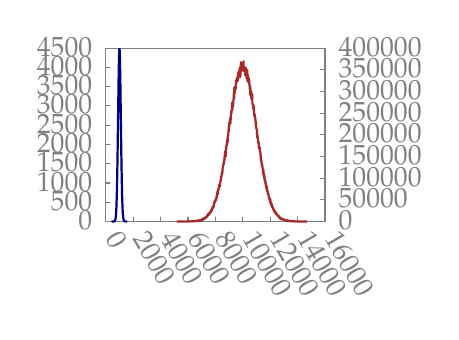
\begin{tikzpicture}[gnuplot, scale=0.3]
%% generated with GNUPLOT 5.2p2 (Lua 5.3; terminal rev. 99, script rev. 102)
%% wo 11 jul 2018 09:51:59 CEST
\path (0.000,0.000) rectangle (12.500,8.750);
\gpcolor{rgb color={0.502,0.502,0.502}}
\gpsetlinetype{gp lt border}
\gpsetdashtype{gp dt solid}
\gpsetlinewidth{1.00}
\draw[gp path] (1.196,1.104)--(1.376,1.104);
\node[gp node right] at (1.012,1.104) {$0$};
\draw[gp path] (1.196,1.919)--(1.376,1.919);
\node[gp node right] at (1.012,1.919) {$500$};
\draw[gp path] (1.196,2.734)--(1.376,2.734);
\node[gp node right] at (1.012,2.734) {$1000$};
\draw[gp path] (1.196,3.550)--(1.376,3.550);
\node[gp node right] at (1.012,3.550) {$1500$};
\draw[gp path] (1.196,4.365)--(1.376,4.365);
\node[gp node right] at (1.012,4.365) {$2000$};
\draw[gp path] (1.196,5.180)--(1.376,5.180);
\node[gp node right] at (1.012,5.180) {$2500$};
\draw[gp path] (1.196,5.995)--(1.376,5.995);
\node[gp node right] at (1.012,5.995) {$3000$};
\draw[gp path] (1.196,6.811)--(1.376,6.811);
\node[gp node right] at (1.012,6.811) {$3500$};
\draw[gp path] (1.196,7.626)--(1.376,7.626);
\node[gp node right] at (1.012,7.626) {$4000$};
\draw[gp path] (1.196,8.441)--(1.376,8.441);
\node[gp node right] at (1.012,8.441) {$4500$};
\draw[gp path] (1.196,1.104)--(1.196,1.284);
\node[gp node left,rotate=-60] at (1.196,0.920) {$0$};
\draw[gp path] (2.356,1.104)--(2.356,1.284);
\node[gp node left,rotate=-60] at (2.356,0.920) {$2000$};
\draw[gp path] (3.516,1.104)--(3.516,1.284);
\node[gp node left,rotate=-60] at (3.516,0.920) {$4000$};
\draw[gp path] (4.676,1.104)--(4.676,1.284);
\node[gp node left,rotate=-60] at (4.676,0.920) {$6000$};
\draw[gp path] (5.836,1.104)--(5.836,1.284);
\node[gp node left,rotate=-60] at (5.836,0.920) {$8000$};
\draw[gp path] (6.995,1.104)--(6.995,1.284);
\node[gp node left,rotate=-60] at (6.995,0.920) {$10000$};
\draw[gp path] (8.155,1.104)--(8.155,1.284);
\node[gp node left,rotate=-60] at (8.155,0.920) {$12000$};
\draw[gp path] (9.315,1.104)--(9.315,1.284);
\node[gp node left,rotate=-60] at (9.315,0.920) {$14000$};
\draw[gp path] (10.475,1.104)--(10.475,1.284);
\node[gp node left,rotate=-60] at (10.475,0.920) {$16000$};
\draw[gp path] (10.475,1.104)--(10.295,1.104);
\node[gp node left] at (10.659,1.104) {$0$};
\draw[gp path] (10.475,2.021)--(10.295,2.021);
\node[gp node left] at (10.659,2.021) {$50000$};
\draw[gp path] (10.475,2.938)--(10.295,2.938);
\node[gp node left] at (10.659,2.938) {$100000$};
\draw[gp path] (10.475,3.855)--(10.295,3.855);
\node[gp node left] at (10.659,3.855) {$150000$};
\draw[gp path] (10.475,4.773)--(10.295,4.773);
\node[gp node left] at (10.659,4.773) {$200000$};
\draw[gp path] (10.475,5.690)--(10.295,5.690);
\node[gp node left] at (10.659,5.690) {$250000$};
\draw[gp path] (10.475,6.607)--(10.295,6.607);
\node[gp node left] at (10.659,6.607) {$300000$};
\draw[gp path] (10.475,7.524)--(10.295,7.524);
\node[gp node left] at (10.659,7.524) {$350000$};
\draw[gp path] (10.475,8.441)--(10.295,8.441);
\node[gp node left] at (10.659,8.441) {$400000$};
\draw[gp path] (1.196,8.441)--(1.196,1.104)--(10.475,1.104)--(10.475,8.441)--cycle;
\gpcolor{rgb color={0.647,0.165,0.165}}
\gpsetlinewidth{2.00}
\draw[gp path] (4.217,1.106)--(4.241,1.106)--(4.264,1.106)--(4.304,1.106)--(4.310,1.106)%
  --(4.339,1.106)--(4.351,1.106)--(4.362,1.106)--(4.403,1.106)--(4.432,1.106)--(4.449,1.106)%
  --(4.473,1.106)--(4.484,1.106)--(4.490,1.106)--(4.513,1.109)--(4.525,1.106)--(4.531,1.106)%
  --(4.536,1.109)--(4.542,1.107)--(4.548,1.107)--(4.554,1.106)--(4.565,1.106)--(4.571,1.107)%
  --(4.577,1.106)--(4.583,1.107)--(4.612,1.106)--(4.618,1.106)--(4.623,1.106)--(4.647,1.106)%
  --(4.652,1.106)--(4.658,1.111)--(4.664,1.106)--(4.670,1.109)--(4.676,1.107)--(4.681,1.107)%
  --(4.687,1.106)--(4.693,1.106)--(4.699,1.112)--(4.705,1.109)--(4.710,1.107)--(4.722,1.111)%
  --(4.728,1.107)--(4.734,1.106)--(4.739,1.106)--(4.745,1.114)--(4.751,1.107)--(4.757,1.112)%
  --(4.763,1.111)--(4.768,1.109)--(4.774,1.114)--(4.780,1.109)--(4.786,1.106)--(4.797,1.106)%
  --(4.803,1.109)--(4.809,1.109)--(4.815,1.112)--(4.821,1.112)--(4.826,1.112)--(4.832,1.119)%
  --(4.838,1.111)--(4.844,1.111)--(4.850,1.111)--(4.855,1.111)--(4.861,1.112)--(4.867,1.112)%
  --(4.873,1.112)--(4.879,1.114)--(4.884,1.114)--(4.890,1.112)--(4.896,1.106)--(4.902,1.114)%
  --(4.908,1.107)--(4.913,1.112)--(4.919,1.119)--(4.925,1.117)--(4.931,1.112)--(4.937,1.114)%
  --(4.942,1.120)--(4.948,1.112)--(4.954,1.115)--(4.960,1.114)--(4.966,1.117)--(4.971,1.115)%
  --(4.977,1.120)--(4.983,1.117)--(4.989,1.120)--(4.995,1.120)--(5.000,1.128)--(5.006,1.128)%
  --(5.012,1.122)--(5.018,1.125)--(5.024,1.122)--(5.029,1.125)--(5.035,1.120)--(5.041,1.143)%
  --(5.047,1.132)--(5.053,1.117)--(5.058,1.125)--(5.064,1.124)--(5.070,1.143)--(5.076,1.127)%
  --(5.082,1.137)--(5.087,1.125)--(5.093,1.140)--(5.099,1.138)--(5.105,1.150)--(5.111,1.143)%
  --(5.116,1.127)--(5.122,1.148)--(5.128,1.138)--(5.134,1.138)--(5.140,1.122)--(5.145,1.151)%
  --(5.151,1.155)--(5.157,1.150)--(5.163,1.156)--(5.169,1.159)--(5.174,1.161)--(5.180,1.145)%
  --(5.186,1.127)--(5.192,1.171)--(5.198,1.153)--(5.203,1.137)--(5.209,1.163)--(5.215,1.161)%
  --(5.221,1.176)--(5.227,1.159)--(5.232,1.148)--(5.238,1.161)--(5.244,1.176)--(5.250,1.161)%
  --(5.256,1.181)--(5.261,1.186)--(5.267,1.186)--(5.273,1.172)--(5.279,1.179)--(5.285,1.189)%
  --(5.290,1.181)--(5.296,1.200)--(5.302,1.230)--(5.308,1.177)--(5.314,1.199)--(5.319,1.203)%
  --(5.325,1.195)--(5.331,1.215)--(5.337,1.192)--(5.343,1.238)--(5.348,1.217)--(5.354,1.225)%
  --(5.360,1.231)--(5.366,1.254)--(5.372,1.233)--(5.377,1.221)--(5.383,1.249)--(5.389,1.244)%
  --(5.395,1.234)--(5.401,1.236)--(5.406,1.278)--(5.412,1.265)--(5.418,1.283)--(5.424,1.262)%
  --(5.430,1.277)--(5.435,1.288)--(5.441,1.275)--(5.447,1.305)--(5.453,1.319)--(5.459,1.296)%
  --(5.464,1.305)--(5.470,1.313)--(5.476,1.303)--(5.482,1.305)--(5.488,1.378)--(5.493,1.327)%
  --(5.499,1.370)--(5.505,1.360)--(5.511,1.347)--(5.517,1.373)--(5.522,1.376)--(5.528,1.368)%
  --(5.534,1.443)--(5.540,1.394)--(5.546,1.368)--(5.551,1.391)--(5.557,1.401)--(5.563,1.442)%
  --(5.569,1.450)--(5.575,1.412)--(5.580,1.437)--(5.586,1.474)--(5.592,1.468)--(5.598,1.487)%
  --(5.604,1.453)--(5.609,1.484)--(5.615,1.487)--(5.621,1.510)--(5.627,1.469)--(5.633,1.487)%
  --(5.638,1.534)--(5.644,1.561)--(5.650,1.531)--(5.656,1.585)--(5.662,1.601)--(5.667,1.543)%
  --(5.673,1.619)--(5.679,1.590)--(5.685,1.554)--(5.691,1.655)--(5.696,1.645)--(5.702,1.626)%
  --(5.708,1.680)--(5.714,1.724)--(5.720,1.696)--(5.725,1.701)--(5.731,1.704)--(5.737,1.667)%
  --(5.743,1.738)--(5.749,1.694)--(5.754,1.727)--(5.760,1.751)--(5.766,1.746)--(5.772,1.836)%
  --(5.778,1.916)--(5.783,1.895)--(5.789,1.916)--(5.795,1.909)--(5.801,1.895)--(5.807,1.905)%
  --(5.812,1.981)--(5.818,1.993)--(5.824,1.940)--(5.830,1.960)--(5.836,2.011)--(5.841,2.020)%
  --(5.847,2.007)--(5.853,2.012)--(5.859,2.014)--(5.864,2.074)--(5.870,2.012)--(5.876,2.128)%
  --(5.882,2.182)--(5.888,2.157)--(5.893,2.198)--(5.899,2.113)--(5.905,2.236)--(5.911,2.262)%
  --(5.917,2.319)--(5.922,2.291)--(5.928,2.381)--(5.934,2.297)--(5.940,2.412)--(5.946,2.271)%
  --(5.951,2.389)--(5.957,2.426)--(5.963,2.506)--(5.969,2.439)--(5.975,2.529)--(5.980,2.496)%
  --(5.986,2.580)--(5.992,2.655)--(5.998,2.630)--(6.004,2.597)--(6.009,2.674)--(6.015,2.679)%
  --(6.021,2.659)--(6.027,2.584)--(6.033,2.739)--(6.038,2.792)--(6.044,2.792)--(6.050,2.798)%
  --(6.056,2.809)--(6.062,2.907)--(6.067,2.932)--(6.073,2.919)--(6.079,3.010)--(6.085,2.972)%
  --(6.091,3.005)--(6.096,3.072)--(6.102,3.108)--(6.108,3.145)--(6.114,3.188)--(6.120,3.111)%
  --(6.125,3.214)--(6.131,3.196)--(6.137,3.331)--(6.143,3.364)--(6.149,3.388)--(6.154,3.444)%
  --(6.160,3.460)--(6.166,3.488)--(6.172,3.522)--(6.178,3.563)--(6.183,3.550)--(6.189,3.517)%
  --(6.195,3.672)--(6.201,3.718)--(6.207,3.654)--(6.212,3.687)--(6.218,3.716)--(6.224,3.837)%
  --(6.230,3.902)--(6.236,3.806)--(6.241,3.933)--(6.247,4.070)--(6.253,3.939)--(6.259,3.996)%
  --(6.265,4.084)--(6.270,3.850)--(6.276,4.143)--(6.282,4.174)--(6.288,4.143)--(6.294,4.156)%
  --(6.299,4.309)--(6.305,4.305)--(6.311,4.318)--(6.317,4.340)--(6.323,4.541)--(6.328,4.342)%
  --(6.334,4.464)--(6.340,4.552)--(6.346,4.611)--(6.352,4.438)--(6.357,4.544)--(6.363,4.720)%
  --(6.369,4.766)--(6.375,4.738)--(6.381,4.773)--(6.386,4.942)--(6.392,4.937)--(6.398,4.945)%
  --(6.404,5.120)--(6.410,4.916)--(6.415,5.126)--(6.421,5.117)--(6.427,5.312)--(6.433,5.294)%
  --(6.439,5.328)--(6.444,5.351)--(6.450,5.275)--(6.456,5.469)--(6.462,5.283)--(6.468,5.417)%
  --(6.473,5.253)--(6.479,5.443)--(6.485,5.588)--(6.491,5.421)--(6.497,5.509)--(6.502,5.673)%
  --(6.508,5.777)--(6.514,5.677)--(6.520,5.808)--(6.526,5.790)--(6.531,5.806)--(6.537,5.995)%
  --(6.543,5.945)--(6.549,6.157)--(6.555,5.888)--(6.560,5.821)--(6.566,6.054)--(6.572,6.157)%
  --(6.578,6.002)--(6.584,5.974)--(6.589,6.087)--(6.595,6.209)--(6.601,6.299)--(6.607,6.277)%
  --(6.613,6.532)--(6.618,6.281)--(6.624,6.367)--(6.630,6.775)--(6.636,6.359)--(6.642,6.628)%
  --(6.647,6.636)--(6.653,6.586)--(6.659,6.643)--(6.665,6.776)--(6.671,6.811)--(6.676,6.678)%
  --(6.682,6.762)--(6.688,6.732)--(6.694,6.739)--(6.700,6.913)--(6.705,7.075)--(6.711,7.021)%
  --(6.717,7.008)--(6.723,7.089)--(6.729,6.975)--(6.734,7.114)--(6.740,7.148)--(6.746,7.071)%
  --(6.752,7.065)--(6.758,7.207)--(6.763,7.155)--(6.769,7.086)--(6.775,7.042)--(6.781,7.094)%
  --(6.787,7.215)--(6.792,7.336)--(6.798,7.163)--(6.804,7.412)--(6.810,7.340)--(6.816,7.383)%
  --(6.821,7.357)--(6.827,7.256)--(6.833,7.383)--(6.839,7.477)--(6.845,7.303)--(6.850,7.225)%
  --(6.856,7.428)--(6.862,7.621)--(6.868,7.476)--(6.874,7.451)--(6.879,7.520)--(6.885,7.551)%
  --(6.891,7.226)--(6.897,7.404)--(6.903,7.425)--(6.908,7.420)--(6.914,7.846)--(6.920,7.466)%
  --(6.926,7.616)--(6.932,7.593)--(6.937,7.580)--(6.943,7.577)--(6.949,7.500)--(6.955,7.792)%
  --(6.961,7.593)--(6.966,7.619)--(6.972,7.650)--(6.978,7.629)--(6.984,7.711)--(6.990,7.660)%
  --(6.995,7.701)--(7.001,7.614)--(7.007,7.484)--(7.013,7.554)--(7.019,7.657)--(7.024,7.888)%
  --(7.030,7.562)--(7.036,7.554)--(7.042,7.510)--(7.048,7.508)--(7.053,7.652)--(7.059,7.481)%
  --(7.065,7.552)--(7.071,7.645)--(7.077,7.484)--(7.082,7.500)--(7.088,7.561)--(7.094,7.300)%
  --(7.100,7.517)--(7.106,7.510)--(7.111,7.411)--(7.117,7.611)--(7.123,7.473)--(7.129,7.468)%
  --(7.135,7.424)--(7.140,7.448)--(7.146,7.376)--(7.152,7.220)--(7.158,7.164)--(7.164,7.420)%
  --(7.169,7.221)--(7.175,7.308)--(7.181,7.520)--(7.187,7.274)--(7.193,7.037)--(7.198,7.244)%
  --(7.204,7.019)--(7.210,7.318)--(7.216,7.128)--(7.222,7.200)--(7.227,7.076)--(7.233,7.096)%
  --(7.239,7.111)--(7.245,7.190)--(7.251,7.075)--(7.256,7.125)--(7.262,7.117)--(7.268,6.918)%
  --(7.274,6.928)--(7.280,6.869)--(7.285,6.804)--(7.291,6.726)--(7.297,6.708)--(7.303,6.731)%
  --(7.309,6.837)--(7.314,6.455)--(7.320,6.649)--(7.326,6.667)--(7.332,6.458)--(7.338,6.636)%
  --(7.343,6.646)--(7.349,6.450)--(7.355,6.349)--(7.361,6.579)--(7.367,6.277)--(7.372,6.308)%
  --(7.378,6.307)--(7.384,6.452)--(7.390,6.289)--(7.396,6.481)--(7.401,6.105)--(7.407,6.069)%
  --(7.413,6.064)--(7.419,6.074)--(7.425,5.999)--(7.430,5.901)--(7.436,6.031)--(7.442,5.909)%
  --(7.448,5.852)--(7.454,5.853)--(7.459,6.000)--(7.465,5.792)--(7.471,5.723)--(7.477,5.668)%
  --(7.483,5.591)--(7.488,5.547)--(7.494,5.663)--(7.500,5.581)--(7.506,5.557)--(7.512,5.518)%
  --(7.517,5.513)--(7.523,5.462)--(7.529,5.417)--(7.535,5.322)--(7.541,5.311)--(7.546,5.143)%
  --(7.552,5.327)--(7.558,5.149)--(7.564,5.050)--(7.570,5.058)--(7.575,5.061)--(7.581,4.981)%
  --(7.587,4.991)--(7.593,4.958)--(7.599,4.790)--(7.604,4.653)--(7.610,4.746)--(7.616,4.781)%
  --(7.622,4.701)--(7.628,4.606)--(7.633,4.624)--(7.639,4.494)--(7.645,4.505)--(7.651,4.427)%
  --(7.657,4.477)--(7.662,4.412)--(7.668,4.464)--(7.674,4.218)--(7.680,4.262)--(7.686,4.285)%
  --(7.691,4.199)--(7.697,4.215)--(7.703,4.164)--(7.709,4.243)--(7.714,4.156)--(7.720,4.018)%
  --(7.726,4.065)--(7.732,4.037)--(7.738,4.040)--(7.743,3.939)--(7.749,3.925)--(7.755,3.894)%
  --(7.761,3.667)--(7.767,3.838)--(7.772,3.701)--(7.778,3.634)--(7.784,3.646)--(7.790,3.608)%
  --(7.796,3.465)--(7.801,3.504)--(7.807,3.468)--(7.813,3.546)--(7.819,3.467)--(7.825,3.439)%
  --(7.830,3.427)--(7.836,3.336)--(7.842,3.259)--(7.848,3.325)--(7.854,3.160)--(7.859,3.243)%
  --(7.865,3.109)--(7.871,3.268)--(7.877,3.145)--(7.883,3.046)--(7.888,3.021)--(7.894,3.057)%
  --(7.900,2.932)--(7.906,3.116)--(7.912,2.943)--(7.917,2.894)--(7.923,2.836)--(7.929,2.912)%
  --(7.935,2.822)--(7.941,2.774)--(7.946,2.783)--(7.952,2.813)--(7.958,2.686)--(7.964,2.749)%
  --(7.970,2.645)--(7.975,2.676)--(7.981,2.617)--(7.987,2.630)--(7.993,2.511)--(7.999,2.506)%
  --(8.004,2.612)--(8.010,2.436)--(8.016,2.482)--(8.022,2.493)--(8.028,2.426)--(8.033,2.379)%
  --(8.039,2.428)--(8.045,2.358)--(8.051,2.257)--(8.057,2.363)--(8.062,2.240)--(8.068,2.325)%
  --(8.074,2.249)--(8.080,2.278)--(8.086,2.244)--(8.091,2.161)--(8.097,2.126)--(8.103,2.164)%
  --(8.109,2.086)--(8.115,2.143)--(8.120,2.092)--(8.126,2.020)--(8.132,2.055)--(8.138,2.009)%
  --(8.144,2.004)--(8.149,1.924)--(8.155,1.980)--(8.161,2.059)--(8.167,1.869)--(8.173,1.882)%
  --(8.178,1.846)--(8.184,1.869)--(8.190,1.903)--(8.196,1.892)--(8.202,1.784)--(8.207,1.833)%
  --(8.213,1.807)--(8.219,1.818)--(8.225,1.758)--(8.231,1.834)--(8.236,1.711)--(8.242,1.748)%
  --(8.248,1.683)--(8.254,1.704)--(8.260,1.684)--(8.265,1.704)--(8.271,1.684)--(8.277,1.676)%
  --(8.283,1.631)--(8.289,1.649)--(8.294,1.596)--(8.300,1.640)--(8.306,1.593)--(8.312,1.557)%
  --(8.318,1.582)--(8.323,1.513)--(8.329,1.559)--(8.335,1.574)--(8.341,1.512)--(8.347,1.507)%
  --(8.352,1.515)--(8.358,1.525)--(8.364,1.523)--(8.370,1.500)--(8.376,1.469)--(8.381,1.477)%
  --(8.387,1.414)--(8.393,1.500)--(8.399,1.451)--(8.405,1.448)--(8.410,1.445)--(8.416,1.435)%
  --(8.422,1.402)--(8.428,1.409)--(8.434,1.412)--(8.439,1.401)--(8.445,1.407)--(8.451,1.384)%
  --(8.457,1.394)--(8.463,1.362)--(8.468,1.384)--(8.474,1.352)--(8.480,1.360)--(8.486,1.342)%
  --(8.492,1.314)--(8.497,1.322)--(8.503,1.308)--(8.509,1.309)--(8.515,1.339)--(8.521,1.339)%
  --(8.526,1.274)--(8.532,1.295)--(8.538,1.293)--(8.544,1.303)--(8.550,1.274)--(8.555,1.249)%
  --(8.561,1.244)--(8.567,1.278)--(8.573,1.230)--(8.579,1.257)--(8.584,1.254)--(8.590,1.249)%
  --(8.596,1.231)--(8.602,1.246)--(8.608,1.252)--(8.613,1.194)--(8.619,1.243)--(8.625,1.231)%
  --(8.631,1.212)--(8.637,1.215)--(8.642,1.212)--(8.648,1.199)--(8.654,1.195)--(8.660,1.190)%
  --(8.666,1.197)--(8.671,1.189)--(8.677,1.208)--(8.683,1.202)--(8.689,1.189)--(8.695,1.192)%
  --(8.700,1.179)--(8.706,1.208)--(8.712,1.187)--(8.718,1.177)--(8.724,1.176)--(8.729,1.164)%
  --(8.735,1.195)--(8.741,1.171)--(8.747,1.161)--(8.753,1.179)--(8.758,1.159)--(8.764,1.164)%
  --(8.770,1.176)--(8.776,1.159)--(8.782,1.168)--(8.787,1.155)--(8.793,1.153)--(8.799,1.163)%
  --(8.805,1.169)--(8.811,1.172)--(8.816,1.158)--(8.822,1.163)--(8.828,1.148)--(8.834,1.146)%
  --(8.840,1.153)--(8.845,1.138)--(8.851,1.137)--(8.857,1.146)--(8.863,1.140)--(8.869,1.137)%
  --(8.874,1.138)--(8.880,1.158)--(8.886,1.148)--(8.892,1.132)--(8.898,1.138)--(8.903,1.135)%
  --(8.909,1.132)--(8.915,1.142)--(8.921,1.138)--(8.927,1.125)--(8.932,1.128)--(8.938,1.132)%
  --(8.944,1.122)--(8.950,1.125)--(8.956,1.127)--(8.961,1.124)--(8.967,1.142)--(8.973,1.119)%
  --(8.979,1.114)--(8.985,1.122)--(8.990,1.120)--(8.996,1.122)--(9.002,1.128)--(9.008,1.117)%
  --(9.014,1.120)--(9.019,1.112)--(9.025,1.117)--(9.031,1.117)--(9.037,1.119)--(9.043,1.119)%
  --(9.048,1.119)--(9.054,1.124)--(9.060,1.124)--(9.066,1.115)--(9.072,1.120)--(9.077,1.112)%
  --(9.083,1.115)--(9.089,1.119)--(9.095,1.114)--(9.101,1.114)--(9.106,1.115)--(9.112,1.111)%
  --(9.118,1.112)--(9.124,1.111)--(9.130,1.107)--(9.135,1.114)--(9.141,1.114)--(9.147,1.106)%
  --(9.153,1.112)--(9.159,1.112)--(9.164,1.107)--(9.170,1.114)--(9.176,1.112)--(9.182,1.109)%
  --(9.188,1.111)--(9.193,1.107)--(9.199,1.109)--(9.205,1.109)--(9.211,1.107)--(9.222,1.106)%
  --(9.228,1.106)--(9.240,1.109)--(9.246,1.106)--(9.251,1.106)--(9.257,1.109)--(9.263,1.106)%
  --(9.275,1.107)--(9.280,1.106)--(9.286,1.106)--(9.292,1.106)--(9.298,1.107)--(9.304,1.107)%
  --(9.309,1.107)--(9.315,1.107)--(9.321,1.107)--(9.327,1.109)--(9.333,1.106)--(9.338,1.106)%
  --(9.344,1.107)--(9.350,1.106)--(9.356,1.107)--(9.362,1.106)--(9.396,1.107)--(9.431,1.107)%
  --(9.443,1.106)--(9.454,1.107)--(9.460,1.107)--(9.472,1.106)--(9.478,1.106)--(9.495,1.106)%
  --(9.507,1.106)--(9.518,1.106)--(9.547,1.106)--(9.698,1.106);
\gpcolor{rgb color={0.000,0.000,0.502}}
\draw[gp path] (1.463,1.104)--(1.480,1.104)--(1.486,1.104)--(1.492,1.104)--(1.498,1.104)%
  --(1.503,1.104)--(1.509,1.104)--(1.515,1.104)--(1.521,1.105)--(1.527,1.105)--(1.532,1.106)%
  --(1.538,1.106)--(1.544,1.107)--(1.550,1.109)--(1.556,1.111)--(1.561,1.113)--(1.567,1.117)%
  --(1.573,1.123)--(1.579,1.131)--(1.585,1.140)--(1.590,1.153)--(1.596,1.172)--(1.602,1.198)%
  --(1.608,1.228)--(1.614,1.265)--(1.619,1.321)--(1.625,1.382)--(1.631,1.467)--(1.637,1.562)%
  --(1.643,1.677)--(1.648,1.823)--(1.654,1.989)--(1.660,2.194)--(1.666,2.416)--(1.672,2.677)%
  --(1.677,2.980)--(1.683,3.297)--(1.689,3.641)--(1.695,4.035)--(1.701,4.432)--(1.706,4.869)%
  --(1.712,5.297)--(1.718,5.730)--(1.724,6.162)--(1.730,6.608)--(1.735,7.026)--(1.741,7.372)%
  --(1.747,7.689)--(1.753,7.953)--(1.759,8.186)--(1.764,8.338)--(1.770,8.400)--(1.776,8.405)%
  --(1.782,8.342)--(1.788,8.211)--(1.793,8.003)--(1.799,7.754)--(1.805,7.408)--(1.811,7.033)%
  --(1.817,6.654)--(1.822,6.231)--(1.828,5.801)--(1.834,5.329)--(1.840,4.892)--(1.846,4.477)%
  --(1.851,4.071)--(1.857,3.681)--(1.863,3.324)--(1.869,2.994)--(1.875,2.701)--(1.880,2.437)%
  --(1.886,2.210)--(1.892,2.003)--(1.898,1.840)--(1.904,1.689)--(1.909,1.572)--(1.915,1.476)%
  --(1.921,1.390)--(1.927,1.325)--(1.933,1.270)--(1.938,1.234)--(1.944,1.200)--(1.950,1.176)%
  --(1.956,1.156)--(1.962,1.142)--(1.967,1.131)--(1.973,1.123)--(1.979,1.118)--(1.985,1.114)%
  --(1.991,1.110)--(1.996,1.108)--(2.002,1.107)--(2.008,1.106)--(2.014,1.105)--(2.020,1.105)%
  --(2.025,1.105)--(2.031,1.104)--(2.037,1.104)--(2.043,1.104)--(2.049,1.104)--(2.060,1.104)%
  --(2.066,1.104)--(2.072,1.104)--(2.078,1.104);
%% coordinates of the plot area
\gpdefrectangularnode{gp plot 1}{\pgfpoint{1.196cm}{1.104cm}}{\pgfpoint{10.475cm}{8.441cm}}
\end{tikzpicture}
%% gnuplot variables

\end{tabular}
\end{center}
\caption{\label{fig:inputselection:normal_10to1_randomOn}
  \texttt{Random-Improve} with a 10:1 deposit:payment ratio, both normally
  distributed.
}
\end{figure}

We see a very similar picture as we did in
Figure~\ref{fig:inputselection:normal_3to1_randomOn}. Since the deposits and
payments are randomly drawn (from normal distributions), the UTxO balance
naturally fluctuates up and down. What is satisfying to see however is that the
\emph{size} of the UTxO tracks the balance rather precisely; this is about as
good as we can hope for. Notice also that the change:payment ratio is a nice
round 1, and the average number of transaction inputs covers around 10 or 11,
which is what we'd expect for a 10:1 ratio of deposits:payments.

\subsubsection{Exponential distribution, 1:1 deposit:payment ratio}
\label{sec:inputselection:erlang1_1to1_randomOn}

What if the payments and deposits are not normally distributed?
Figure~\ref{fig:inputselection:erlang1_1to1_randomOn} shows
\texttt{Random-Improve} on exponentially distributed inputs. In an exponential
distribution we have a lot of values near 0; for such values it will be hard to
achieve a `good' change output, as we are likely to overshoot the range. Partly
due to this reason the algorithm isn't quite achieving a 1.0 change:payment
ratio, but at 1.5 it is still generating useful change outputs. Furthermore, we
can see that the size of the UTxO tracks the UTxO balance nicely, and the
average number of transaction inputs is low, with roughly 53\% having just one
input. Moreover, when we increase the deposit:payment ratio to 3:1 and then
10:0, the change:payment ratio drops to about 1.1 and then back to 1.0 (graphs
omitted).

\begin{figure}[p]
\begin{center}
\scriptsize
\begin{tabular}{ll}
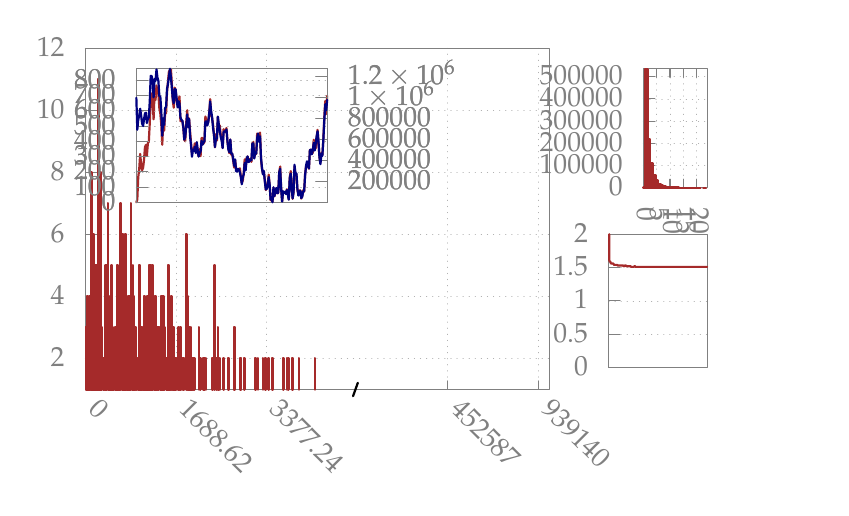
\begin{tikzpicture}[gnuplot, xscale=0.8, yscale=0.6]
%% generated with GNUPLOT 5.2p2 (Lua 5.3; terminal rev. 99, script rev. 102)
%% wo 11 jul 2018 11:20:48 CEST
\path (0.000,0.000) rectangle (12.500,8.750);
\gpcolor{color=gp lt color axes}
\gpsetlinetype{gp lt axes}
\gpsetdashtype{gp dt axes}
\gpsetlinewidth{0.50}
\draw[gp path] (0.828,1.875)--(8.197,1.875);
\gpcolor{rgb color={0.502,0.502,0.502}}
\gpsetlinetype{gp lt border}
\gpsetdashtype{gp dt solid}
\gpsetlinewidth{1.00}
\draw[gp path] (0.828,1.875)--(1.008,1.875);
\node[gp node right] at (0.644,1.875) {$2$};
\gpcolor{color=gp lt color axes}
\gpsetlinetype{gp lt axes}
\gpsetdashtype{gp dt axes}
\gpsetlinewidth{0.50}
\draw[gp path] (0.828,3.188)--(8.197,3.188);
\gpcolor{rgb color={0.502,0.502,0.502}}
\gpsetlinetype{gp lt border}
\gpsetdashtype{gp dt solid}
\gpsetlinewidth{1.00}
\draw[gp path] (0.828,3.188)--(1.008,3.188);
\node[gp node right] at (0.644,3.188) {$4$};
\gpcolor{color=gp lt color axes}
\gpsetlinetype{gp lt axes}
\gpsetdashtype{gp dt axes}
\gpsetlinewidth{0.50}
\draw[gp path] (0.828,4.501)--(8.197,4.501);
\gpcolor{rgb color={0.502,0.502,0.502}}
\gpsetlinetype{gp lt border}
\gpsetdashtype{gp dt solid}
\gpsetlinewidth{1.00}
\draw[gp path] (0.828,4.501)--(1.008,4.501);
\node[gp node right] at (0.644,4.501) {$6$};
\gpcolor{color=gp lt color axes}
\gpsetlinetype{gp lt axes}
\gpsetdashtype{gp dt axes}
\gpsetlinewidth{0.50}
\draw[gp path] (0.828,5.814)--(8.197,5.814);
\gpcolor{rgb color={0.502,0.502,0.502}}
\gpsetlinetype{gp lt border}
\gpsetdashtype{gp dt solid}
\gpsetlinewidth{1.00}
\draw[gp path] (0.828,5.814)--(1.008,5.814);
\node[gp node right] at (0.644,5.814) {$8$};
\gpcolor{color=gp lt color axes}
\gpsetlinetype{gp lt axes}
\gpsetdashtype{gp dt axes}
\gpsetlinewidth{0.50}
\draw[gp path] (0.828,7.128)--(8.197,7.128);
\gpcolor{rgb color={0.502,0.502,0.502}}
\gpsetlinetype{gp lt border}
\gpsetdashtype{gp dt solid}
\gpsetlinewidth{1.00}
\draw[gp path] (0.828,7.128)--(1.008,7.128);
\node[gp node right] at (0.644,7.128) {$10$};
\gpcolor{color=gp lt color axes}
\gpsetlinetype{gp lt axes}
\gpsetdashtype{gp dt axes}
\gpsetlinewidth{0.50}
\draw[gp path] (0.828,8.441)--(8.197,8.441);
\gpcolor{rgb color={0.502,0.502,0.502}}
\gpsetlinetype{gp lt border}
\gpsetdashtype{gp dt solid}
\gpsetlinewidth{1.00}
\draw[gp path] (0.828,8.441)--(1.008,8.441);
\node[gp node right] at (0.644,8.441) {$12$};
\gpcolor{color=gp lt color axes}
\gpsetlinetype{gp lt axes}
\gpsetdashtype{gp dt axes}
\gpsetlinewidth{0.50}
\draw[gp path] (0.828,1.218)--(0.828,8.441);
\gpcolor{rgb color={0.502,0.502,0.502}}
\gpsetlinetype{gp lt border}
\gpsetdashtype{gp dt solid}
\gpsetlinewidth{1.00}
\draw[gp path] (0.828,1.218)--(0.828,1.398);
\node[gp node left,rotate=-45] at (0.828,1.034) {$0$};
\gpcolor{color=gp lt color axes}
\gpsetlinetype{gp lt axes}
\gpsetdashtype{gp dt axes}
\gpsetlinewidth{0.50}
\draw[gp path] (2.266,1.218)--(2.266,8.441);
\gpcolor{rgb color={0.502,0.502,0.502}}
\gpsetlinetype{gp lt border}
\gpsetdashtype{gp dt solid}
\gpsetlinewidth{1.00}
\draw[gp path] (2.266,1.218)--(2.266,1.398);
\node[gp node left,rotate=-45] at (2.266,1.034) {$1688.62$};
\gpcolor{color=gp lt color axes}
\gpsetlinetype{gp lt axes}
\gpsetdashtype{gp dt axes}
\gpsetlinewidth{0.50}
\draw[gp path] (3.704,1.218)--(3.704,8.441);
\gpcolor{rgb color={0.502,0.502,0.502}}
\gpsetlinetype{gp lt border}
\gpsetdashtype{gp dt solid}
\gpsetlinewidth{1.00}
\draw[gp path] (3.704,1.218)--(3.704,1.398);
\node[gp node left,rotate=-45] at (3.704,1.034) {$3377.24$};
\gpcolor{color=gp lt color axes}
\gpsetlinetype{gp lt axes}
\gpsetdashtype{gp dt axes}
\gpsetlinewidth{0.50}
% commented out since this exceeds tikz bounds
% \draw[gp path] (-2147483.648,1.218)--(-2147483.648,8.441);
\draw[gp path] (6.579,1.218)--(6.579,8.441);
\gpcolor{rgb color={0.502,0.502,0.502}}
\gpsetlinetype{gp lt border}
\gpsetdashtype{gp dt solid}
\gpsetlinewidth{1.00}
\draw[gp path] (6.579,1.218)--(6.579,1.398);
\node[gp node left,rotate=-45] at (6.579,1.034) {$452587$};
\gpcolor{color=gp lt color axes}
\gpsetlinetype{gp lt axes}
\gpsetdashtype{gp dt axes}
\gpsetlinewidth{0.50}
\draw[gp path] (8.017,1.218)--(8.017,8.441);
\gpcolor{rgb color={0.502,0.502,0.502}}
\gpsetlinetype{gp lt border}
\gpsetdashtype{gp dt solid}
\gpsetlinewidth{1.00}
\draw[gp path] (8.017,1.218)--(8.017,1.398);
\node[gp node left,rotate=-45] at (8.017,1.034) {$939140$};
\draw[gp path] (0.828,8.441)--(0.828,1.218)--(8.197,1.218)--(8.197,8.441)--cycle;
\gpcolor{rgb color={0.647,0.165,0.165}}
\gpsetlinewidth{2.00}
\draw[gp path] (0.832,1.218)--(0.832,2.531)--(0.841,2.531)--(0.841,1.218)--cycle;
\draw[gp path] (0.841,1.218)--(0.841,2.531)--(0.849,2.531)--(0.849,1.218)--cycle;
\draw[gp path] (0.849,1.218)--(0.849,1.875)--(0.858,1.875)--(0.858,1.218)--cycle;
\draw[gp path] (0.858,1.218)--(0.858,3.188)--(0.866,3.188)--(0.866,1.218)--cycle;
\draw[gp path] (0.866,1.218)--(0.866,2.531)--(0.875,2.531)--(0.875,1.218)--cycle;
\draw[gp path] (0.875,1.218)--(0.875,2.531)--(0.883,2.531)--(0.883,1.218)--cycle;
\draw[gp path] (0.883,1.218)--(0.883,2.531)--(0.892,2.531)--(0.892,1.218)--cycle;
\draw[gp path] (0.892,1.218)--(0.892,3.188)--(0.900,3.188)--(0.900,1.218)--cycle;
\draw[gp path] (0.909,1.218)--(0.909,2.531)--(0.917,2.531)--(0.917,1.218)--cycle;
\draw[gp path] (0.917,1.218)--(0.917,5.814)--(0.926,5.814)--(0.926,1.218)--cycle;
\draw[gp path] (0.926,1.218)--(0.926,1.875)--(0.934,1.875)--(0.934,1.218)--cycle;
\draw[gp path] (0.934,1.218)--(0.934,1.875)--(0.943,1.875)--(0.943,1.218)--cycle;
\draw[gp path] (0.943,1.218)--(0.943,3.845)--(0.951,3.845)--(0.951,1.218)--cycle;
\draw[gp path] (0.951,1.218)--(0.951,4.501)--(0.960,4.501)--(0.960,1.218)--cycle;
\draw[gp path] (0.960,1.218)--(0.960,2.531)--(0.968,2.531)--(0.968,1.218)--cycle;
\draw[gp path] (0.968,1.218)--(0.968,3.188)--(0.977,3.188)--(0.977,1.218)--cycle;
\draw[gp path] (0.977,1.218)--(0.977,3.845)--(0.986,3.845)--(0.986,1.218)--cycle;
\draw[gp path] (0.986,1.218)--(0.986,3.845)--(0.994,3.845)--(0.994,1.218)--cycle;
\draw[gp path] (0.994,1.218)--(0.994,3.845)--(1.003,3.845)--(1.003,1.218)--cycle;
\draw[gp path] (1.003,1.218)--(1.003,3.188)--(1.011,3.188)--(1.011,1.218)--cycle;
\draw[gp path] (1.011,1.218)--(1.011,1.875)--(1.020,1.875)--(1.020,1.218)--cycle;
\draw[gp path] (1.020,1.218)--(1.020,2.531)--(1.028,2.531)--(1.028,1.218)--cycle;
\draw[gp path] (1.028,1.218)--(1.028,7.784)--(1.037,7.784)--(1.037,1.218)--cycle;
\draw[gp path] (1.037,1.218)--(1.037,3.188)--(1.045,3.188)--(1.045,1.218)--cycle;
\draw[gp path] (1.045,1.218)--(1.045,3.188)--(1.054,3.188)--(1.054,1.218)--cycle;
\draw[gp path] (1.054,1.218)--(1.054,2.531)--(1.062,2.531)--(1.062,1.218)--cycle;
\draw[gp path] (1.062,1.218)--(1.062,5.814)--(1.071,5.814)--(1.071,1.218)--cycle;
\draw[gp path] (1.079,1.218)--(1.079,2.531)--(1.088,2.531)--(1.088,1.218)--cycle;
\draw[gp path] (1.113,1.218)--(1.113,1.875)--(1.122,1.875)--(1.122,1.218)--cycle;
\draw[gp path] (1.122,1.218)--(1.122,1.875)--(1.130,1.875)--(1.130,1.218)--cycle;
\draw[gp path] (1.139,1.218)--(1.139,2.531)--(1.147,2.531)--(1.147,1.218)--cycle;
\draw[gp path] (1.147,1.218)--(1.147,3.845)--(1.156,3.845)--(1.156,1.218)--cycle;
\draw[gp path] (1.156,1.218)--(1.156,3.845)--(1.164,3.845)--(1.164,1.218)--cycle;
\draw[gp path] (1.164,1.218)--(1.164,1.875)--(1.173,1.875)--(1.173,1.218)--cycle;
\draw[gp path] (1.181,1.218)--(1.181,5.158)--(1.190,5.158)--(1.190,1.218)--cycle;
\draw[gp path] (1.190,1.218)--(1.190,2.531)--(1.198,2.531)--(1.198,1.218)--cycle;
\draw[gp path] (1.198,1.218)--(1.198,2.531)--(1.207,2.531)--(1.207,1.218)--cycle;
\draw[gp path] (1.207,1.218)--(1.207,2.531)--(1.215,2.531)--(1.215,1.218)--cycle;
\draw[gp path] (1.215,1.218)--(1.215,2.531)--(1.224,2.531)--(1.224,1.218)--cycle;
\draw[gp path] (1.224,1.218)--(1.224,3.188)--(1.232,3.188)--(1.232,1.218)--cycle;
\draw[gp path] (1.232,1.218)--(1.232,3.188)--(1.241,3.188)--(1.241,1.218)--cycle;
\draw[gp path] (1.241,1.218)--(1.241,3.845)--(1.249,3.845)--(1.249,1.218)--cycle;
\draw[gp path] (1.249,1.218)--(1.249,1.875)--(1.258,1.875)--(1.258,1.218)--cycle;
\draw[gp path] (1.258,1.218)--(1.258,2.531)--(1.267,2.531)--(1.267,1.218)--cycle;
\draw[gp path] (1.267,1.218)--(1.267,1.875)--(1.275,1.875)--(1.275,1.218)--cycle;
\draw[gp path] (1.275,1.218)--(1.275,1.875)--(1.284,1.875)--(1.284,1.218)--cycle;
\draw[gp path] (1.292,1.218)--(1.292,1.875)--(1.301,1.875)--(1.301,1.218)--cycle;
\draw[gp path] (1.301,1.218)--(1.301,2.531)--(1.309,2.531)--(1.309,1.218)--cycle;
\draw[gp path] (1.309,1.218)--(1.309,1.875)--(1.318,1.875)--(1.318,1.218)--cycle;
\draw[gp path] (1.318,1.218)--(1.318,2.531)--(1.326,2.531)--(1.326,1.218)--cycle;
\draw[gp path] (1.326,1.218)--(1.326,1.875)--(1.335,1.875)--(1.335,1.218)--cycle;
\draw[gp path] (1.335,1.218)--(1.335,3.845)--(1.343,3.845)--(1.343,1.218)--cycle;
\draw[gp path] (1.343,1.218)--(1.343,2.531)--(1.352,2.531)--(1.352,1.218)--cycle;
\draw[gp path] (1.352,1.218)--(1.352,3.188)--(1.360,3.188)--(1.360,1.218)--cycle;
\draw[gp path] (1.360,1.218)--(1.360,2.531)--(1.369,2.531)--(1.369,1.218)--cycle;
\draw[gp path] (1.369,1.218)--(1.369,2.531)--(1.377,2.531)--(1.377,1.218)--cycle;
\draw[gp path] (1.386,1.218)--(1.386,5.158)--(1.394,5.158)--(1.394,1.218)--cycle;
\draw[gp path] (1.403,1.218)--(1.403,3.188)--(1.411,3.188)--(1.411,1.218)--cycle;
\draw[gp path] (1.411,1.218)--(1.411,4.501)--(1.420,4.501)--(1.420,1.218)--cycle;
\draw[gp path] (1.420,1.218)--(1.420,4.501)--(1.428,4.501)--(1.428,1.218)--cycle;
\draw[gp path] (1.428,1.218)--(1.428,1.875)--(1.437,1.875)--(1.437,1.218)--cycle;
\draw[gp path] (1.437,1.218)--(1.437,3.188)--(1.445,3.188)--(1.445,1.218)--cycle;
\draw[gp path] (1.445,1.218)--(1.445,3.188)--(1.454,3.188)--(1.454,1.218)--cycle;
\draw[gp path] (1.454,1.218)--(1.454,2.531)--(1.462,2.531)--(1.462,1.218)--cycle;
\draw[gp path] (1.462,1.218)--(1.462,4.501)--(1.471,4.501)--(1.471,1.218)--cycle;
\draw[gp path] (1.471,1.218)--(1.471,2.531)--(1.479,2.531)--(1.479,1.218)--cycle;
\draw[gp path] (1.488,1.218)--(1.488,1.875)--(1.496,1.875)--(1.496,1.218)--cycle;
\draw[gp path] (1.496,1.218)--(1.496,2.531)--(1.505,2.531)--(1.505,1.218)--cycle;
\draw[gp path] (1.505,1.218)--(1.505,3.188)--(1.513,3.188)--(1.513,1.218)--cycle;
\draw[gp path] (1.513,1.218)--(1.513,2.531)--(1.522,2.531)--(1.522,1.218)--cycle;
\draw[gp path] (1.522,1.218)--(1.522,3.188)--(1.530,3.188)--(1.530,1.218)--cycle;
\draw[gp path] (1.530,1.218)--(1.530,1.875)--(1.539,1.875)--(1.539,1.218)--cycle;
\draw[gp path] (1.539,1.218)--(1.539,3.188)--(1.548,3.188)--(1.548,1.218)--cycle;
\draw[gp path] (1.548,1.218)--(1.548,5.158)--(1.556,5.158)--(1.556,1.218)--cycle;
\draw[gp path] (1.573,1.218)--(1.573,2.531)--(1.582,2.531)--(1.582,1.218)--cycle;
\draw[gp path] (1.582,1.218)--(1.582,3.845)--(1.590,3.845)--(1.590,1.218)--cycle;
\draw[gp path] (1.590,1.218)--(1.590,3.188)--(1.599,3.188)--(1.599,1.218)--cycle;
\draw[gp path] (1.599,1.218)--(1.599,2.531)--(1.607,2.531)--(1.607,1.218)--cycle;
\draw[gp path] (1.607,1.218)--(1.607,1.875)--(1.616,1.875)--(1.616,1.218)--cycle;
\draw[gp path] (1.624,1.218)--(1.624,2.531)--(1.633,2.531)--(1.633,1.218)--cycle;
\draw[gp path] (1.641,1.218)--(1.641,1.875)--(1.650,1.875)--(1.650,1.218)--cycle;
\draw[gp path] (1.658,1.218)--(1.658,1.875)--(1.667,1.875)--(1.667,1.218)--cycle;
\draw[gp path] (1.667,1.218)--(1.667,1.875)--(1.675,1.875)--(1.675,1.218)--cycle;
\draw[gp path] (1.675,1.218)--(1.675,1.875)--(1.684,1.875)--(1.684,1.218)--cycle;
\draw[gp path] (1.684,1.218)--(1.684,3.845)--(1.692,3.845)--(1.692,1.218)--cycle;
\draw[gp path] (1.701,1.218)--(1.701,1.875)--(1.709,1.875)--(1.709,1.218)--cycle;
\draw[gp path] (1.709,1.218)--(1.709,1.875)--(1.718,1.875)--(1.718,1.218)--cycle;
\draw[gp path] (1.718,1.218)--(1.718,2.531)--(1.726,2.531)--(1.726,1.218)--cycle;
\draw[gp path] (1.726,1.218)--(1.726,1.875)--(1.735,1.875)--(1.735,1.218)--cycle;
\draw[gp path] (1.743,1.218)--(1.743,2.531)--(1.752,2.531)--(1.752,1.218)--cycle;
\draw[gp path] (1.752,1.218)--(1.752,1.875)--(1.760,1.875)--(1.760,1.218)--cycle;
\draw[gp path] (1.760,1.218)--(1.760,3.188)--(1.769,3.188)--(1.769,1.218)--cycle;
\draw[gp path] (1.769,1.218)--(1.769,2.531)--(1.777,2.531)--(1.777,1.218)--cycle;
\draw[gp path] (1.777,1.218)--(1.777,1.875)--(1.786,1.875)--(1.786,1.218)--cycle;
\draw[gp path] (1.786,1.218)--(1.786,2.531)--(1.794,2.531)--(1.794,1.218)--cycle;
\draw[gp path] (1.794,1.218)--(1.794,1.875)--(1.803,1.875)--(1.803,1.218)--cycle;
\draw[gp path] (1.811,1.218)--(1.811,3.188)--(1.820,3.188)--(1.820,1.218)--cycle;
\draw[gp path] (1.820,1.218)--(1.820,3.188)--(1.829,3.188)--(1.829,1.218)--cycle;
\draw[gp path] (1.829,1.218)--(1.829,2.531)--(1.837,2.531)--(1.837,1.218)--cycle;
\draw[gp path] (1.837,1.218)--(1.837,3.845)--(1.846,3.845)--(1.846,1.218)--cycle;
\draw[gp path] (1.846,1.218)--(1.846,1.875)--(1.854,1.875)--(1.854,1.218)--cycle;
\draw[gp path] (1.854,1.218)--(1.854,1.875)--(1.863,1.875)--(1.863,1.218)--cycle;
\draw[gp path] (1.863,1.218)--(1.863,3.845)--(1.871,3.845)--(1.871,1.218)--cycle;
\draw[gp path] (1.871,1.218)--(1.871,1.875)--(1.880,1.875)--(1.880,1.218)--cycle;
\draw[gp path] (1.880,1.218)--(1.880,3.188)--(1.888,3.188)--(1.888,1.218)--cycle;
\draw[gp path] (1.888,1.218)--(1.888,3.845)--(1.897,3.845)--(1.897,1.218)--cycle;
\draw[gp path] (1.914,1.218)--(1.914,3.188)--(1.922,3.188)--(1.922,1.218)--cycle;
\draw[gp path] (1.922,1.218)--(1.922,1.875)--(1.931,1.875)--(1.931,1.218)--cycle;
\draw[gp path] (1.931,1.218)--(1.931,2.531)--(1.939,2.531)--(1.939,1.218)--cycle;
\draw[gp path] (1.939,1.218)--(1.939,3.188)--(1.948,3.188)--(1.948,1.218)--cycle;
\draw[gp path] (1.948,1.218)--(1.948,2.531)--(1.956,2.531)--(1.956,1.218)--cycle;
\draw[gp path] (1.956,1.218)--(1.956,2.531)--(1.965,2.531)--(1.965,1.218)--cycle;
\draw[gp path] (1.973,1.218)--(1.973,2.531)--(1.982,2.531)--(1.982,1.218)--cycle;
\draw[gp path] (1.982,1.218)--(1.982,2.531)--(1.990,2.531)--(1.990,1.218)--cycle;
\draw[gp path] (1.990,1.218)--(1.990,2.531)--(1.999,2.531)--(1.999,1.218)--cycle;
\draw[gp path] (2.016,1.218)--(2.016,2.531)--(2.024,2.531)--(2.024,1.218)--cycle;
\draw[gp path] (2.024,1.218)--(2.024,1.875)--(2.033,1.875)--(2.033,1.218)--cycle;
\draw[gp path] (2.033,1.218)--(2.033,3.188)--(2.041,3.188)--(2.041,1.218)--cycle;
\draw[gp path] (2.050,1.218)--(2.050,3.188)--(2.058,3.188)--(2.058,1.218)--cycle;
\draw[gp path] (2.058,1.218)--(2.058,3.188)--(2.067,3.188)--(2.067,1.218)--cycle;
\draw[gp path] (2.067,1.218)--(2.067,2.531)--(2.075,2.531)--(2.075,1.218)--cycle;
\draw[gp path] (2.075,1.218)--(2.075,2.531)--(2.084,2.531)--(2.084,1.218)--cycle;
\draw[gp path] (2.110,1.218)--(2.110,1.875)--(2.118,1.875)--(2.118,1.218)--cycle;
\draw[gp path] (2.118,1.218)--(2.118,1.875)--(2.127,1.875)--(2.127,1.218)--cycle;
\draw[gp path] (2.127,1.218)--(2.127,1.875)--(2.135,1.875)--(2.135,1.218)--cycle;
\draw[gp path] (2.135,1.218)--(2.135,1.875)--(2.144,1.875)--(2.144,1.218)--cycle;
\draw[gp path] (2.144,1.218)--(2.144,3.845)--(2.152,3.845)--(2.152,1.218)--cycle;
\draw[gp path] (2.161,1.218)--(2.161,1.875)--(2.169,1.875)--(2.169,1.218)--cycle;
\draw[gp path] (2.169,1.218)--(2.169,1.875)--(2.178,1.875)--(2.178,1.218)--cycle;
\draw[gp path] (2.186,1.218)--(2.186,3.188)--(2.195,3.188)--(2.195,1.218)--cycle;
\draw[gp path] (2.212,1.218)--(2.212,2.531)--(2.220,2.531)--(2.220,1.218)--cycle;
\draw[gp path] (2.220,1.218)--(2.220,2.531)--(2.229,2.531)--(2.229,1.218)--cycle;
\draw[gp path] (2.229,1.218)--(2.229,1.875)--(2.237,1.875)--(2.237,1.218)--cycle;
\draw[gp path] (2.237,1.218)--(2.237,1.875)--(2.246,1.875)--(2.246,1.218)--cycle;
\draw[gp path] (2.254,1.218)--(2.254,1.875)--(2.263,1.875)--(2.263,1.218)--cycle;
\draw[gp path] (2.263,1.218)--(2.263,1.875)--(2.271,1.875)--(2.271,1.218)--cycle;
\draw[gp path] (2.280,1.218)--(2.280,1.875)--(2.288,1.875)--(2.288,1.218)--cycle;
\draw[gp path] (2.297,1.218)--(2.297,1.875)--(2.305,1.875)--(2.305,1.218)--cycle;
\draw[gp path] (2.305,1.218)--(2.305,2.531)--(2.314,2.531)--(2.314,1.218)--cycle;
\draw[gp path] (2.322,1.218)--(2.322,1.875)--(2.331,1.875)--(2.331,1.218)--cycle;
\draw[gp path] (2.331,1.218)--(2.331,1.875)--(2.339,1.875)--(2.339,1.218)--cycle;
\draw[gp path] (2.339,1.218)--(2.339,2.531)--(2.348,2.531)--(2.348,1.218)--cycle;
\draw[gp path] (2.356,1.218)--(2.356,1.875)--(2.365,1.875)--(2.365,1.218)--cycle;
\draw[gp path] (2.373,1.218)--(2.373,1.875)--(2.382,1.875)--(2.382,1.218)--cycle;
\draw[gp path] (2.382,1.218)--(2.382,1.875)--(2.390,1.875)--(2.390,1.218)--cycle;
\draw[gp path] (2.390,1.218)--(2.390,1.875)--(2.399,1.875)--(2.399,1.218)--cycle;
\draw[gp path] (2.425,1.218)--(2.425,4.501)--(2.433,4.501)--(2.433,1.218)--cycle;
\draw[gp path] (2.450,1.218)--(2.450,3.188)--(2.459,3.188)--(2.459,1.218)--cycle;
\draw[gp path] (2.459,1.218)--(2.459,1.875)--(2.467,1.875)--(2.467,1.218)--cycle;
\draw[gp path] (2.467,1.218)--(2.467,1.875)--(2.476,1.875)--(2.476,1.218)--cycle;
\draw[gp path] (2.476,1.218)--(2.476,2.531)--(2.484,2.531)--(2.484,1.218)--cycle;
\draw[gp path] (2.493,1.218)--(2.493,1.875)--(2.501,1.875)--(2.501,1.218)--cycle;
\draw[gp path] (2.501,1.218)--(2.501,2.531)--(2.510,2.531)--(2.510,1.218)--cycle;
\draw[gp path] (2.510,1.218)--(2.510,1.875)--(2.518,1.875)--(2.518,1.218)--cycle;
\draw[gp path] (2.518,1.218)--(2.518,1.875)--(2.527,1.875)--(2.527,1.218)--cycle;
\draw[gp path] (2.535,1.218)--(2.535,1.875)--(2.544,1.875)--(2.544,1.218)--cycle;
\draw[gp path] (2.552,1.218)--(2.552,1.875)--(2.561,1.875)--(2.561,1.218)--cycle;
\draw[gp path] (2.629,1.218)--(2.629,2.531)--(2.637,2.531)--(2.637,1.218)--cycle;
\draw[gp path] (2.646,1.218)--(2.646,1.875)--(2.654,1.875)--(2.654,1.218)--cycle;
\draw[gp path] (2.697,1.218)--(2.697,1.875)--(2.706,1.875)--(2.706,1.218)--cycle;
\draw[gp path] (2.714,1.218)--(2.714,1.875)--(2.723,1.875)--(2.723,1.218)--cycle;
\draw[gp path] (2.740,1.218)--(2.740,1.875)--(2.748,1.875)--(2.748,1.218)--cycle;
\draw[gp path] (2.842,1.218)--(2.842,1.875)--(2.850,1.875)--(2.850,1.218)--cycle;
\draw[gp path] (2.876,1.218)--(2.876,3.845)--(2.884,3.845)--(2.884,1.218)--cycle;
\draw[gp path] (2.910,1.218)--(2.910,1.875)--(2.918,1.875)--(2.918,1.218)--cycle;
\draw[gp path] (2.927,1.218)--(2.927,2.531)--(2.935,2.531)--(2.935,1.218)--cycle;
\draw[gp path] (2.935,1.218)--(2.935,1.875)--(2.944,1.875)--(2.944,1.218)--cycle;
\draw[gp path] (2.944,1.218)--(2.944,1.875)--(2.952,1.875)--(2.952,1.218)--cycle;
\draw[gp path] (2.961,1.218)--(2.961,1.875)--(2.970,1.875)--(2.970,1.218)--cycle;
\draw[gp path] (3.021,1.218)--(3.021,1.875)--(3.029,1.875)--(3.029,1.218)--cycle;
\draw[gp path] (3.097,1.218)--(3.097,1.875)--(3.106,1.875)--(3.106,1.218)--cycle;
\draw[gp path] (3.182,1.218)--(3.182,1.875)--(3.191,1.875)--(3.191,1.218)--cycle;
\draw[gp path] (3.191,1.218)--(3.191,2.531)--(3.199,2.531)--(3.199,1.218)--cycle;
\draw[gp path] (3.285,1.218)--(3.285,1.875)--(3.293,1.875)--(3.293,1.218)--cycle;
\draw[gp path] (3.293,1.218)--(3.293,1.875)--(3.302,1.875)--(3.302,1.218)--cycle;
\draw[gp path] (3.344,1.218)--(3.344,1.875)--(3.353,1.875)--(3.353,1.218)--cycle;
\draw[gp path] (3.523,1.218)--(3.523,1.875)--(3.532,1.875)--(3.532,1.218)--cycle;
\draw[gp path] (3.566,1.218)--(3.566,1.875)--(3.574,1.875)--(3.574,1.218)--cycle;
\draw[gp path] (3.642,1.218)--(3.642,1.875)--(3.651,1.875)--(3.651,1.218)--cycle;
\draw[gp path] (3.685,1.218)--(3.685,1.875)--(3.693,1.875)--(3.693,1.218)--cycle;
\draw[gp path] (3.736,1.218)--(3.736,1.875)--(3.744,1.875)--(3.744,1.218)--cycle;
\draw[gp path] (3.795,1.218)--(3.795,1.875)--(3.804,1.875)--(3.804,1.218)--cycle;
\draw[gp path] (3.966,1.218)--(3.966,1.875)--(3.974,1.875)--(3.974,1.218)--cycle;
\draw[gp path] (4.025,1.218)--(4.025,1.875)--(4.034,1.875)--(4.034,1.218)--cycle;
\draw[gp path] (4.042,1.218)--(4.042,1.875)--(4.051,1.875)--(4.051,1.218)--cycle;
\draw[gp path] (4.111,1.218)--(4.111,1.875)--(4.119,1.875)--(4.119,1.218)--cycle;
\draw[gp path] (4.213,1.218)--(4.213,1.875)--(4.221,1.875)--(4.221,1.218)--cycle;
\draw[gp path] (4.468,1.218)--(4.468,1.875)--(4.477,1.875)--(4.477,1.218)--cycle;
\gpcolor{color=gp lt color border}
\draw[gp path](5.077,1.074)--(5.153,1.358);
%% coordinates of the plot area
\gpdefrectangularnode{gp plot 1}{\pgfpoint{0.828cm}{1.218cm}}{\pgfpoint{8.197cm}{8.441cm}}
\gpcolor{color=gp lt color axes}
\gpsetlinetype{gp lt axes}
\gpsetdashtype{gp dt axes}
\gpsetlinewidth{0.50}
\draw[gp path] (1.637,5.177)--(4.666,5.177);
\gpcolor{rgb color={0.502,0.502,0.502}}
\gpsetlinetype{gp lt border}
\gpsetdashtype{gp dt solid}
\gpsetlinewidth{1.00}
\draw[gp path] (1.637,5.177)--(1.817,5.177);
\node[gp node right] at (1.453,5.177) {$0$};
\gpcolor{color=gp lt color axes}
\gpsetlinetype{gp lt axes}
\gpsetdashtype{gp dt axes}
\gpsetlinewidth{0.50}
\draw[gp path] (1.637,5.500)--(4.666,5.500);
\gpcolor{rgb color={0.502,0.502,0.502}}
\gpsetlinetype{gp lt border}
\gpsetdashtype{gp dt solid}
\gpsetlinewidth{1.00}
\draw[gp path] (1.637,5.500)--(1.817,5.500);
\node[gp node right] at (1.453,5.500) {$100$};
\gpcolor{color=gp lt color axes}
\gpsetlinetype{gp lt axes}
\gpsetdashtype{gp dt axes}
\gpsetlinewidth{0.50}
\draw[gp path] (1.637,5.822)--(4.666,5.822);
\gpcolor{rgb color={0.502,0.502,0.502}}
\gpsetlinetype{gp lt border}
\gpsetdashtype{gp dt solid}
\gpsetlinewidth{1.00}
\draw[gp path] (1.637,5.822)--(1.817,5.822);
\node[gp node right] at (1.453,5.822) {$200$};
\gpcolor{color=gp lt color axes}
\gpsetlinetype{gp lt axes}
\gpsetdashtype{gp dt axes}
\gpsetlinewidth{0.50}
\draw[gp path] (1.637,6.145)--(4.666,6.145);
\gpcolor{rgb color={0.502,0.502,0.502}}
\gpsetlinetype{gp lt border}
\gpsetdashtype{gp dt solid}
\gpsetlinewidth{1.00}
\draw[gp path] (1.637,6.145)--(1.817,6.145);
\node[gp node right] at (1.453,6.145) {$300$};
\gpcolor{color=gp lt color axes}
\gpsetlinetype{gp lt axes}
\gpsetdashtype{gp dt axes}
\gpsetlinewidth{0.50}
\draw[gp path] (1.637,6.468)--(4.666,6.468);
\gpcolor{rgb color={0.502,0.502,0.502}}
\gpsetlinetype{gp lt border}
\gpsetdashtype{gp dt solid}
\gpsetlinewidth{1.00}
\draw[gp path] (1.637,6.468)--(1.817,6.468);
\node[gp node right] at (1.453,6.468) {$400$};
\gpcolor{color=gp lt color axes}
\gpsetlinetype{gp lt axes}
\gpsetdashtype{gp dt axes}
\gpsetlinewidth{0.50}
\draw[gp path] (1.637,6.790)--(4.666,6.790);
\gpcolor{rgb color={0.502,0.502,0.502}}
\gpsetlinetype{gp lt border}
\gpsetdashtype{gp dt solid}
\gpsetlinewidth{1.00}
\draw[gp path] (1.637,6.790)--(1.817,6.790);
\node[gp node right] at (1.453,6.790) {$500$};
\gpcolor{color=gp lt color axes}
\gpsetlinetype{gp lt axes}
\gpsetdashtype{gp dt axes}
\gpsetlinewidth{0.50}
\draw[gp path] (1.637,7.113)--(4.666,7.113);
\gpcolor{rgb color={0.502,0.502,0.502}}
\gpsetlinetype{gp lt border}
\gpsetdashtype{gp dt solid}
\gpsetlinewidth{1.00}
\draw[gp path] (1.637,7.113)--(1.817,7.113);
\node[gp node right] at (1.453,7.113) {$600$};
\gpcolor{color=gp lt color axes}
\gpsetlinetype{gp lt axes}
\gpsetdashtype{gp dt axes}
\gpsetlinewidth{0.50}
\draw[gp path] (1.637,7.436)--(4.666,7.436);
\gpcolor{rgb color={0.502,0.502,0.502}}
\gpsetlinetype{gp lt border}
\gpsetdashtype{gp dt solid}
\gpsetlinewidth{1.00}
\draw[gp path] (1.637,7.436)--(1.817,7.436);
\node[gp node right] at (1.453,7.436) {$700$};
\gpcolor{color=gp lt color axes}
\gpsetlinetype{gp lt axes}
\gpsetdashtype{gp dt axes}
\gpsetlinewidth{0.50}
\draw[gp path] (1.637,7.759)--(4.666,7.759);
\gpcolor{rgb color={0.502,0.502,0.502}}
\gpsetlinetype{gp lt border}
\gpsetdashtype{gp dt solid}
\gpsetlinewidth{1.00}
\draw[gp path] (1.637,7.759)--(1.817,7.759);
\node[gp node right] at (1.453,7.759) {$800$};
\draw[gp path] (4.666,5.618)--(4.486,5.618);
\node[gp node left] at (4.850,5.618) {$200000$};
\draw[gp path] (4.666,6.061)--(4.486,6.061);
\node[gp node left] at (4.850,6.061) {$400000$};
\draw[gp path] (4.666,6.503)--(4.486,6.503);
\node[gp node left] at (4.850,6.503) {$600000$};
\draw[gp path] (4.666,6.946)--(4.486,6.946);
\node[gp node left] at (4.850,6.946) {$800000$};
\draw[gp path] (4.666,7.389)--(4.486,7.389);
\node[gp node left] at (4.850,7.389) {$1\times10^{6}$};
\draw[gp path] (4.666,7.832)--(4.486,7.832);
\node[gp node left] at (4.850,7.832) {$1.2\times10^{6}$};
\draw[gp path] (1.637,8.004)--(1.637,5.180)--(4.666,5.180)--(4.666,8.004)--cycle;
\gpcolor{rgb color={0.647,0.165,0.165}}
\gpsetlinewidth{2.00}
\draw[gp path] (1.637,5.180)--(1.652,5.238)--(1.667,5.713)--(1.683,5.887)--(1.698,6.203)%
  --(1.713,5.977)--(1.728,5.858)--(1.744,5.906)--(1.759,6.084)--(1.774,6.345)--(1.789,6.394)%
  --(1.804,6.161)--(1.820,6.432)--(1.835,6.461)--(1.850,6.858)--(1.865,7.336)--(1.881,7.484)%
  --(1.896,7.297)--(1.911,6.936)--(1.926,7.517)--(1.941,7.342)--(1.957,7.649)--(1.972,7.501)%
  --(1.987,7.478)--(2.002,7.175)--(2.018,7.052)--(2.033,6.826)--(2.048,6.397)--(2.063,6.842)%
  --(2.078,6.694)--(2.094,7.068)--(2.109,7.065)--(2.124,7.513)--(2.139,7.739)--(2.155,7.952)%
  --(2.170,7.917)--(2.185,8.004)--(2.200,7.701)--(2.215,7.329)--(2.231,7.181)--(2.246,7.604)%
  --(2.261,7.555)--(2.276,7.329)--(2.292,7.236)--(2.307,7.326)--(2.322,7.423)--(2.337,6.897)%
  --(2.352,6.913)--(2.368,6.897)--(2.383,6.752)--(2.398,6.503)--(2.413,6.471)--(2.428,6.845)%
  --(2.444,7.126)--(2.459,6.829)--(2.474,6.955)--(2.489,6.700)--(2.505,6.432)--(2.520,6.213)%
  --(2.535,6.310)--(2.550,6.290)--(2.565,6.426)--(2.581,6.316)--(2.596,6.442)--(2.611,6.219)%
  --(2.626,6.151)--(2.642,6.303)--(2.657,6.158)--(2.672,6.539)--(2.687,6.539)--(2.702,6.419)%
  --(2.718,6.455)--(2.733,6.994)--(2.748,6.920)--(2.763,6.855)--(2.779,6.884)--(2.794,7.065)%
  --(2.809,7.362)--(2.824,7.023)--(2.839,6.962)--(2.855,6.823)--(2.870,6.600)--(2.885,6.342)%
  --(2.900,6.619)--(2.916,6.487)--(2.931,6.987)--(2.946,6.765)--(2.961,6.807)--(2.976,6.619)%
  --(2.992,6.548)--(3.007,6.332)--(3.022,6.726)--(3.037,6.668)--(3.053,6.678)--(3.068,6.752)%
  --(3.083,6.461)--(3.098,6.326)--(3.113,6.219)--(3.129,6.506)--(3.144,6.187)--(3.159,6.203)%
  --(3.174,6.064)--(3.190,5.913)--(3.205,6.068)--(3.220,5.900)--(3.235,5.858)--(3.250,5.877)%
  --(3.266,5.880)--(3.281,5.896)--(3.296,5.716)--(3.311,5.587)--(3.327,5.642)--(3.342,5.806)%
  --(3.357,6.087)--(3.372,5.906)--(3.387,6.113)--(3.403,6.148)--(3.418,6.035)--(3.433,6.097)%
  --(3.448,6.093)--(3.464,6.035)--(3.479,6.429)--(3.494,6.458)--(3.509,6.116)--(3.524,6.261)%
  --(3.540,6.200)--(3.555,6.632)--(3.570,6.616)--(3.585,6.484)--(3.601,6.655)--(3.616,6.090)%
  --(3.631,5.896)--(3.646,5.796)--(3.661,5.825)--(3.677,5.642)--(3.692,5.438)--(3.707,5.503)%
  --(3.722,5.545)--(3.738,5.764)--(3.753,5.551)--(3.768,5.222)--(3.783,5.280)--(3.798,5.186)%
  --(3.814,5.490)--(3.829,5.306)--(3.844,5.406)--(3.859,5.470)--(3.875,5.367)--(3.890,5.396)%
  --(3.905,5.813)--(3.920,5.935)--(3.935,5.506)--(3.951,5.196)--(3.966,5.403)--(3.981,5.390)%
  --(3.996,5.390)--(4.011,5.361)--(4.027,5.454)--(4.042,5.377)--(4.057,5.241)--(4.072,5.706)%
  --(4.088,5.838)--(4.103,5.493)--(4.118,5.251)--(4.133,5.387)--(4.148,5.938)--(4.164,5.758)%
  --(4.179,5.767)--(4.194,5.435)--(4.209,5.358)--(4.225,5.432)--(4.240,5.422)--(4.255,5.257)%
  --(4.270,5.309)--(4.285,5.435)--(4.301,5.406)--(4.316,5.777)--(4.331,5.938)--(4.346,5.980)%
  --(4.362,5.990)--(4.377,5.890)--(4.392,6.287)--(4.407,6.290)--(4.422,6.203)--(4.438,6.232)%
  --(4.453,6.503)--(4.468,6.323)--(4.483,6.319)--(4.499,6.542)--(4.514,6.713)--(4.529,6.429)%
  --(4.544,6.129)--(4.559,6.022)--(4.575,6.216)--(4.590,6.177)--(4.605,6.503)--(4.620,6.958)%
  --(4.636,7.323)--(4.651,7.049)--(4.666,7.433);
%% coordinates of the plot area
\gpdefrectangularnode{gp plot 2}{\pgfpoint{1.637cm}{5.180cm}}{\pgfpoint{4.666cm}{8.004cm}}
\gpcolor{color=gp lt color axes}
\gpsetlinetype{gp lt axes}
\gpsetdashtype{gp dt axes}
\gpsetlinewidth{0.50}
\draw[gp path] (1.637,5.177)--(4.666,5.177);
\gpcolor{rgb color={0.502,0.502,0.502}}
\gpsetlinetype{gp lt border}
\gpsetdashtype{gp dt solid}
\gpsetlinewidth{1.00}
\draw[gp path] (1.637,5.177)--(1.817,5.177);
\node[gp node right] at (1.453,5.177) {$0$};
\gpcolor{color=gp lt color axes}
\gpsetlinetype{gp lt axes}
\gpsetdashtype{gp dt axes}
\gpsetlinewidth{0.50}
\draw[gp path] (1.637,5.500)--(4.666,5.500);
\gpcolor{rgb color={0.502,0.502,0.502}}
\gpsetlinetype{gp lt border}
\gpsetdashtype{gp dt solid}
\gpsetlinewidth{1.00}
\draw[gp path] (1.637,5.500)--(1.817,5.500);
\node[gp node right] at (1.453,5.500) {$100$};
\gpcolor{color=gp lt color axes}
\gpsetlinetype{gp lt axes}
\gpsetdashtype{gp dt axes}
\gpsetlinewidth{0.50}
\draw[gp path] (1.637,5.822)--(4.666,5.822);
\gpcolor{rgb color={0.502,0.502,0.502}}
\gpsetlinetype{gp lt border}
\gpsetdashtype{gp dt solid}
\gpsetlinewidth{1.00}
\draw[gp path] (1.637,5.822)--(1.817,5.822);
\node[gp node right] at (1.453,5.822) {$200$};
\gpcolor{color=gp lt color axes}
\gpsetlinetype{gp lt axes}
\gpsetdashtype{gp dt axes}
\gpsetlinewidth{0.50}
\draw[gp path] (1.637,6.145)--(4.666,6.145);
\gpcolor{rgb color={0.502,0.502,0.502}}
\gpsetlinetype{gp lt border}
\gpsetdashtype{gp dt solid}
\gpsetlinewidth{1.00}
\draw[gp path] (1.637,6.145)--(1.817,6.145);
\node[gp node right] at (1.453,6.145) {$300$};
\gpcolor{color=gp lt color axes}
\gpsetlinetype{gp lt axes}
\gpsetdashtype{gp dt axes}
\gpsetlinewidth{0.50}
\draw[gp path] (1.637,6.468)--(4.666,6.468);
\gpcolor{rgb color={0.502,0.502,0.502}}
\gpsetlinetype{gp lt border}
\gpsetdashtype{gp dt solid}
\gpsetlinewidth{1.00}
\draw[gp path] (1.637,6.468)--(1.817,6.468);
\node[gp node right] at (1.453,6.468) {$400$};
\gpcolor{color=gp lt color axes}
\gpsetlinetype{gp lt axes}
\gpsetdashtype{gp dt axes}
\gpsetlinewidth{0.50}
\draw[gp path] (1.637,6.790)--(4.666,6.790);
\gpcolor{rgb color={0.502,0.502,0.502}}
\gpsetlinetype{gp lt border}
\gpsetdashtype{gp dt solid}
\gpsetlinewidth{1.00}
\draw[gp path] (1.637,6.790)--(1.817,6.790);
\node[gp node right] at (1.453,6.790) {$500$};
\gpcolor{color=gp lt color axes}
\gpsetlinetype{gp lt axes}
\gpsetdashtype{gp dt axes}
\gpsetlinewidth{0.50}
\draw[gp path] (1.637,7.113)--(4.666,7.113);
\gpcolor{rgb color={0.502,0.502,0.502}}
\gpsetlinetype{gp lt border}
\gpsetdashtype{gp dt solid}
\gpsetlinewidth{1.00}
\draw[gp path] (1.637,7.113)--(1.817,7.113);
\node[gp node right] at (1.453,7.113) {$600$};
\gpcolor{color=gp lt color axes}
\gpsetlinetype{gp lt axes}
\gpsetdashtype{gp dt axes}
\gpsetlinewidth{0.50}
\draw[gp path] (1.637,7.436)--(4.666,7.436);
\gpcolor{rgb color={0.502,0.502,0.502}}
\gpsetlinetype{gp lt border}
\gpsetdashtype{gp dt solid}
\gpsetlinewidth{1.00}
\draw[gp path] (1.637,7.436)--(1.817,7.436);
\node[gp node right] at (1.453,7.436) {$700$};
\gpcolor{color=gp lt color axes}
\gpsetlinetype{gp lt axes}
\gpsetdashtype{gp dt axes}
\gpsetlinewidth{0.50}
\draw[gp path] (1.637,7.759)--(4.666,7.759);
\gpcolor{rgb color={0.502,0.502,0.502}}
\gpsetlinetype{gp lt border}
\gpsetdashtype{gp dt solid}
\gpsetlinewidth{1.00}
\draw[gp path] (1.637,7.759)--(1.817,7.759);
\node[gp node right] at (1.453,7.759) {$800$};
\draw[gp path] (4.666,5.618)--(4.486,5.618);
\node[gp node left] at (4.850,5.618) {$200000$};
\draw[gp path] (4.666,6.061)--(4.486,6.061);
\node[gp node left] at (4.850,6.061) {$400000$};
\draw[gp path] (4.666,6.503)--(4.486,6.503);
\node[gp node left] at (4.850,6.503) {$600000$};
\draw[gp path] (4.666,6.946)--(4.486,6.946);
\node[gp node left] at (4.850,6.946) {$800000$};
\draw[gp path] (4.666,7.389)--(4.486,7.389);
\node[gp node left] at (4.850,7.389) {$1\times10^{6}$};
\draw[gp path] (4.666,7.832)--(4.486,7.832);
\node[gp node left] at (4.850,7.832) {$1.2\times10^{6}$};
\draw[gp path] (1.637,8.004)--(1.637,5.180)--(4.666,5.180)--(4.666,8.004)--cycle;
\gpcolor{rgb color={0.000,0.000,0.502}}
\gpsetlinewidth{2.00}
\draw[gp path] (1.637,7.389)--(1.652,6.716)--(1.667,6.923)--(1.683,7.017)--(1.698,7.159)%
  --(1.713,7.015)--(1.728,6.847)--(1.744,6.795)--(1.759,6.939)--(1.774,7.058)--(1.789,7.075)%
  --(1.804,6.856)--(1.820,6.942)--(1.835,6.976)--(1.850,7.312)--(1.865,7.855)--(1.881,7.851)%
  --(1.896,7.740)--(1.911,7.402)--(1.926,7.784)--(1.941,7.748)--(1.957,7.991)--(1.972,7.815)%
  --(1.987,7.746)--(2.002,7.432)--(2.018,7.410)--(2.033,7.099)--(2.048,6.588)--(2.063,6.954)%
  --(2.078,6.818)--(2.094,7.180)--(2.109,7.190)--(2.124,7.581)--(2.139,7.680)--(2.155,7.841)%
  --(2.170,8.004)--(2.185,7.834)--(2.200,7.615)--(2.215,7.375)--(2.231,7.275)--(2.246,7.574)%
  --(2.261,7.565)--(2.276,7.381)--(2.292,7.188)--(2.307,7.318)--(2.322,7.266)--(2.337,6.978)%
  --(2.352,6.924)--(2.368,6.903)--(2.383,6.766)--(2.398,6.505)--(2.413,6.565)--(2.428,6.781)%
  --(2.444,7.038)--(2.459,6.770)--(2.474,6.943)--(2.489,6.593)--(2.505,6.384)--(2.520,6.142)%
  --(2.535,6.287)--(2.550,6.265)--(2.565,6.354)--(2.581,6.222)--(2.596,6.448)--(2.611,6.293)%
  --(2.626,6.146)--(2.642,6.224)--(2.657,6.254)--(2.672,6.481)--(2.687,6.398)--(2.702,6.446)%
  --(2.718,6.474)--(2.733,6.884)--(2.748,6.893)--(2.763,6.805)--(2.779,6.874)--(2.794,7.055)%
  --(2.809,7.313)--(2.824,7.109)--(2.839,6.986)--(2.855,6.744)--(2.870,6.605)--(2.885,6.348)%
  --(2.900,6.517)--(2.916,6.526)--(2.931,6.993)--(2.946,6.821)--(2.961,6.699)--(2.976,6.562)%
  --(2.992,6.479)--(3.007,6.326)--(3.022,6.662)--(3.037,6.684)--(3.053,6.675)--(3.068,6.720)%
  --(3.083,6.480)--(3.098,6.293)--(3.113,6.241)--(3.129,6.507)--(3.144,6.209)--(3.159,6.209)%
  --(3.174,6.098)--(3.190,5.948)--(3.205,6.086)--(3.220,5.838)--(3.235,5.829)--(3.250,5.885)%
  --(3.266,5.873)--(3.281,5.811)--(3.296,5.714)--(3.311,5.561)--(3.327,5.706)--(3.342,5.770)%
  --(3.357,6.012)--(3.372,5.856)--(3.387,6.088)--(3.403,6.150)--(3.418,6.031)--(3.433,6.043)%
  --(3.448,6.080)--(3.464,6.068)--(3.479,6.422)--(3.494,6.426)--(3.509,6.106)--(3.524,6.241)%
  --(3.540,6.208)--(3.555,6.545)--(3.570,6.634)--(3.585,6.460)--(3.601,6.575)--(3.616,6.124)%
  --(3.631,5.912)--(3.646,5.769)--(3.661,5.840)--(3.677,5.618)--(3.692,5.451)--(3.707,5.464)%
  --(3.722,5.526)--(3.738,5.714)--(3.753,5.552)--(3.768,5.238)--(3.783,5.284)--(3.798,5.180)%
  --(3.814,5.495)--(3.829,5.310)--(3.844,5.405)--(3.859,5.481)--(3.875,5.372)--(3.890,5.376)%
  --(3.905,5.808)--(3.920,5.890)--(3.935,5.479)--(3.951,5.193)--(3.966,5.412)--(3.981,5.379)%
  --(3.996,5.400)--(4.011,5.356)--(4.027,5.439)--(4.042,5.339)--(4.057,5.234)--(4.072,5.686)%
  --(4.088,5.786)--(4.103,5.466)--(4.118,5.261)--(4.133,5.407)--(4.148,5.972)--(4.164,5.760)%
  --(4.179,5.789)--(4.194,5.465)--(4.209,5.322)--(4.225,5.403)--(4.240,5.427)--(4.255,5.268)%
  --(4.270,5.296)--(4.285,5.406)--(4.301,5.419)--(4.316,5.743)--(4.331,5.952)--(4.346,6.047)%
  --(4.362,5.946)--(4.377,5.895)--(4.392,6.279)--(4.407,6.292)--(4.422,6.194)--(4.438,6.280)%
  --(4.453,6.437)--(4.468,6.275)--(4.483,6.411)--(4.499,6.573)--(4.514,6.682)--(4.529,6.457)%
  --(4.544,6.131)--(4.559,5.986)--(4.575,6.204)--(4.590,6.161)--(4.605,6.483)--(4.620,6.885)%
  --(4.636,7.253)--(4.651,7.129)--(4.666,7.345);
\gpcolor{color=gp lt color axes}
\gpsetlinetype{gp lt axes}
\gpsetdashtype{gp dt axes}
\gpsetlinewidth{0.50}
\draw[gp path] (9.688,5.488)--(10.697,5.488);
\gpcolor{rgb color={0.502,0.502,0.502}}
\gpsetlinetype{gp lt border}
\gpsetdashtype{gp dt solid}
\gpsetlinewidth{1.00}
\draw[gp path] (9.688,5.488)--(9.868,5.488);
\node[gp node right] at (9.504,5.488) {$0$};
\gpcolor{color=gp lt color axes}
\gpsetlinetype{gp lt axes}
\gpsetdashtype{gp dt axes}
\gpsetlinewidth{0.50}
\draw[gp path] (9.688,5.958)--(10.697,5.958);
\gpcolor{rgb color={0.502,0.502,0.502}}
\gpsetlinetype{gp lt border}
\gpsetdashtype{gp dt solid}
\gpsetlinewidth{1.00}
\draw[gp path] (9.688,5.958)--(9.868,5.958);
\node[gp node right] at (9.504,5.958) {$100000$};
\gpcolor{color=gp lt color axes}
\gpsetlinetype{gp lt axes}
\gpsetdashtype{gp dt axes}
\gpsetlinewidth{0.50}
\draw[gp path] (9.688,6.428)--(10.697,6.428);
\gpcolor{rgb color={0.502,0.502,0.502}}
\gpsetlinetype{gp lt border}
\gpsetdashtype{gp dt solid}
\gpsetlinewidth{1.00}
\draw[gp path] (9.688,6.428)--(9.868,6.428);
\node[gp node right] at (9.504,6.428) {$200000$};
\gpcolor{color=gp lt color axes}
\gpsetlinetype{gp lt axes}
\gpsetdashtype{gp dt axes}
\gpsetlinewidth{0.50}
\draw[gp path] (9.688,6.898)--(10.697,6.898);
\gpcolor{rgb color={0.502,0.502,0.502}}
\gpsetlinetype{gp lt border}
\gpsetdashtype{gp dt solid}
\gpsetlinewidth{1.00}
\draw[gp path] (9.688,6.898)--(9.868,6.898);
\node[gp node right] at (9.504,6.898) {$300000$};
\gpcolor{color=gp lt color axes}
\gpsetlinetype{gp lt axes}
\gpsetdashtype{gp dt axes}
\gpsetlinewidth{0.50}
\draw[gp path] (9.688,7.368)--(10.697,7.368);
\gpcolor{rgb color={0.502,0.502,0.502}}
\gpsetlinetype{gp lt border}
\gpsetdashtype{gp dt solid}
\gpsetlinewidth{1.00}
\draw[gp path] (9.688,7.368)--(9.868,7.368);
\node[gp node right] at (9.504,7.368) {$400000$};
\gpcolor{color=gp lt color axes}
\gpsetlinetype{gp lt axes}
\gpsetdashtype{gp dt axes}
\gpsetlinewidth{0.50}
\draw[gp path] (9.688,7.838)--(10.697,7.838);
\gpcolor{rgb color={0.502,0.502,0.502}}
\gpsetlinetype{gp lt border}
\gpsetdashtype{gp dt solid}
\gpsetlinewidth{1.00}
\draw[gp path] (9.688,7.838)--(9.868,7.838);
\node[gp node right] at (9.504,7.838) {$500000$};
\gpcolor{color=gp lt color axes}
\gpsetlinetype{gp lt axes}
\gpsetdashtype{gp dt axes}
\gpsetlinewidth{0.50}
\draw[gp path] (9.688,5.488)--(9.688,7.824)--(9.688,8.004);
\gpcolor{rgb color={0.502,0.502,0.502}}
\gpsetlinetype{gp lt border}
\gpsetdashtype{gp dt solid}
\gpsetlinewidth{1.00}
\draw[gp path] (9.688,5.488)--(9.688,5.668);
\draw[gp path] (9.688,8.004)--(9.688,7.824);
\node[gp node left,rotate=-90] at (9.688,5.304) {$0$};
\gpcolor{color=gp lt color axes}
\gpsetlinetype{gp lt axes}
\gpsetdashtype{gp dt axes}
\gpsetlinewidth{0.50}
\draw[gp path] (9.898,5.488)--(9.898,7.824)--(9.898,8.004);
\gpcolor{rgb color={0.502,0.502,0.502}}
\gpsetlinetype{gp lt border}
\gpsetdashtype{gp dt solid}
\gpsetlinewidth{1.00}
\draw[gp path] (9.898,5.488)--(9.898,5.668);
\draw[gp path] (9.898,8.004)--(9.898,7.824);
\node[gp node left,rotate=-90] at (9.898,5.304) {$5$};
\gpcolor{color=gp lt color axes}
\gpsetlinetype{gp lt axes}
\gpsetdashtype{gp dt axes}
\gpsetlinewidth{0.50}
\draw[gp path] (10.108,5.488)--(10.108,7.824)--(10.108,8.004);
\gpcolor{rgb color={0.502,0.502,0.502}}
\gpsetlinetype{gp lt border}
\gpsetdashtype{gp dt solid}
\gpsetlinewidth{1.00}
\draw[gp path] (10.108,5.488)--(10.108,5.668);
\draw[gp path] (10.108,8.004)--(10.108,7.824);
\node[gp node left,rotate=-90] at (10.108,5.304) {$10$};
\gpcolor{color=gp lt color axes}
\gpsetlinetype{gp lt axes}
\gpsetdashtype{gp dt axes}
\gpsetlinewidth{0.50}
\draw[gp path] (10.319,5.488)--(10.319,7.824)--(10.319,8.004);
\gpcolor{rgb color={0.502,0.502,0.502}}
\gpsetlinetype{gp lt border}
\gpsetdashtype{gp dt solid}
\gpsetlinewidth{1.00}
\draw[gp path] (10.319,5.488)--(10.319,5.668);
\draw[gp path] (10.319,8.004)--(10.319,7.824);
\node[gp node left,rotate=-90] at (10.319,5.304) {$15$};
\gpcolor{color=gp lt color axes}
\gpsetlinetype{gp lt axes}
\gpsetdashtype{gp dt axes}
\gpsetlinewidth{0.50}
\draw[gp path] (10.529,5.488)--(10.529,8.004);
\gpcolor{rgb color={0.502,0.502,0.502}}
\gpsetlinetype{gp lt border}
\gpsetdashtype{gp dt solid}
\gpsetlinewidth{1.00}
\draw[gp path] (10.529,5.488)--(10.529,5.668);
\draw[gp path] (10.529,8.004)--(10.529,7.824);
\node[gp node left,rotate=-90] at (10.529,5.304) {$20$};
\draw[gp path] (9.688,8.004)--(9.688,5.488)--(10.697,5.488)--(10.697,8.004)--cycle;
\gpfill{rgb color={0.647,0.165,0.165}} (9.688,5.488)--(9.710,5.488)--(9.710,5.491)--(9.688,5.491)--cycle;
\gpcolor{rgb color={0.647,0.165,0.165}}
\gpsetlinewidth{2.00}
\draw[gp path] (9.688,5.488)--(9.688,5.490)--(9.709,5.490)--(9.709,5.488)--cycle;
\gpfill{rgb color={0.647,0.165,0.165}} (9.709,5.488)--(9.752,5.488)--(9.752,8.005)--(9.709,8.005)--cycle;
\draw[gp path] (9.709,5.488)--(9.709,8.004)--(9.751,8.004)--(9.751,5.488)--cycle;
\gpfill{rgb color={0.647,0.165,0.165}} (9.751,5.488)--(9.794,5.488)--(9.794,6.523)--(9.751,6.523)--cycle;
\draw[gp path] (9.751,5.488)--(9.751,6.522)--(9.793,6.522)--(9.793,5.488)--cycle;
\gpfill{rgb color={0.647,0.165,0.165}} (9.793,5.488)--(9.836,5.488)--(9.836,5.999)--(9.793,5.999)--cycle;
\draw[gp path] (9.793,5.488)--(9.793,5.998)--(9.835,5.998)--(9.835,5.488)--cycle;
\gpfill{rgb color={0.647,0.165,0.165}} (9.835,5.488)--(9.878,5.488)--(9.878,5.761)--(9.835,5.761)--cycle;
\draw[gp path] (9.835,5.488)--(9.835,5.760)--(9.877,5.760)--(9.877,5.488)--cycle;
\gpfill{rgb color={0.647,0.165,0.165}} (9.877,5.488)--(9.920,5.488)--(9.920,5.640)--(9.877,5.640)--cycle;
\draw[gp path] (9.877,5.488)--(9.877,5.639)--(9.919,5.639)--(9.919,5.488)--cycle;
\gpfill{rgb color={0.647,0.165,0.165}} (9.919,5.488)--(9.962,5.488)--(9.962,5.573)--(9.919,5.573)--cycle;
\draw[gp path] (9.919,5.488)--(9.919,5.572)--(9.961,5.572)--(9.961,5.488)--cycle;
\gpfill{rgb color={0.647,0.165,0.165}} (9.961,5.488)--(10.004,5.488)--(10.004,5.536)--(9.961,5.536)--cycle;
\draw[gp path] (9.961,5.488)--(9.961,5.535)--(10.003,5.535)--(10.003,5.488)--cycle;
\gpfill{rgb color={0.647,0.165,0.165}} (10.003,5.488)--(10.046,5.488)--(10.046,5.515)--(10.003,5.515)--cycle;
\draw[gp path] (10.003,5.488)--(10.003,5.514)--(10.045,5.514)--(10.045,5.488)--cycle;
\gpfill{rgb color={0.647,0.165,0.165}} (10.045,5.488)--(10.088,5.488)--(10.088,5.504)--(10.045,5.504)--cycle;
\draw[gp path] (10.045,5.488)--(10.045,5.503)--(10.087,5.503)--(10.087,5.488)--cycle;
\gpfill{rgb color={0.647,0.165,0.165}} (10.087,5.488)--(10.130,5.488)--(10.130,5.497)--(10.087,5.497)--cycle;
\draw[gp path] (10.087,5.488)--(10.087,5.496)--(10.129,5.496)--(10.129,5.488)--cycle;
\gpfill{rgb color={0.647,0.165,0.165}} (10.129,5.488)--(10.172,5.488)--(10.172,5.494)--(10.129,5.494)--cycle;
\draw[gp path] (10.129,5.488)--(10.129,5.493)--(10.171,5.493)--(10.171,5.488)--cycle;
\gpfill{rgb color={0.647,0.165,0.165}} (10.171,5.488)--(10.215,5.488)--(10.215,5.492)--(10.171,5.492)--cycle;
\draw[gp path] (10.171,5.488)--(10.171,5.491)--(10.214,5.491)--(10.214,5.488)--cycle;
\gpfill{rgb color={0.647,0.165,0.165}} (10.214,5.488)--(10.257,5.488)--(10.257,5.491)--(10.214,5.491)--cycle;
\draw[gp path] (10.214,5.488)--(10.214,5.490)--(10.256,5.490)--(10.256,5.488)--cycle;
\gpfill{rgb color={0.647,0.165,0.165}} (10.256,5.488)--(10.299,5.488)--(10.299,5.490)--(10.256,5.490)--cycle;
\draw[gp path] (10.256,5.488)--(10.256,5.489)--(10.298,5.489)--(10.298,5.488)--cycle;
\gpfill{rgb color={0.647,0.165,0.165}} (10.298,5.488)--(10.341,5.488)--(10.341,5.490)--(10.298,5.490)--cycle;
\draw[gp path] (10.298,5.488)--(10.298,5.489)--(10.340,5.489)--(10.340,5.488)--cycle;
\gpfill{rgb color={0.647,0.165,0.165}} (10.340,5.488)--(10.383,5.488)--(10.383,5.489)--(10.340,5.489)--cycle;
\draw[gp path] (10.340,5.488)--(10.382,5.488)--cycle;
\gpfill{rgb color={0.647,0.165,0.165}} (10.382,5.488)--(10.425,5.488)--(10.425,5.489)--(10.382,5.489)--cycle;
\draw[gp path] (10.382,5.488)--(10.424,5.488)--cycle;
\gpfill{rgb color={0.647,0.165,0.165}} (10.424,5.488)--(10.467,5.488)--(10.467,5.489)--(10.424,5.489)--cycle;
\draw[gp path] (10.424,5.488)--(10.466,5.488)--cycle;
\gpfill{rgb color={0.647,0.165,0.165}} (10.466,5.488)--(10.509,5.488)--(10.509,5.489)--(10.466,5.489)--cycle;
\draw[gp path] (10.466,5.488)--(10.508,5.488)--cycle;
\gpfill{rgb color={0.647,0.165,0.165}} (10.508,5.488)--(10.551,5.488)--(10.551,5.489)--(10.508,5.489)--cycle;
\draw[gp path] (10.508,5.488)--(10.550,5.488)--cycle;
\gpfill{rgb color={0.647,0.165,0.165}} (10.550,5.488)--(10.593,5.488)--(10.593,5.489)--(10.550,5.489)--cycle;
\draw[gp path] (10.550,5.488)--(10.592,5.488)--cycle;
\gpfill{rgb color={0.647,0.165,0.165}} (10.634,5.488)--(10.677,5.488)--(10.677,5.489)--(10.634,5.489)--cycle;
\draw[gp path] (10.634,5.488)--(10.676,5.488)--cycle;
%% coordinates of the plot area
\gpdefrectangularnode{gp plot 3}{\pgfpoint{9.688cm}{5.488cm}}{\pgfpoint{10.697cm}{8.004cm}}
\gpcolor{color=gp lt color axes}
\gpsetlinetype{gp lt axes}
\gpsetdashtype{gp dt axes}
\gpsetlinewidth{0.50}
\draw[gp path] (9.136,1.680)--(10.697,1.680);
\gpcolor{rgb color={0.502,0.502,0.502}}
\gpsetlinetype{gp lt border}
\gpsetdashtype{gp dt solid}
\gpsetlinewidth{1.00}
\draw[gp path] (9.136,1.680)--(9.316,1.680);
\node[gp node right] at (8.952,1.680) {$0$};
\gpcolor{color=gp lt color axes}
\gpsetlinetype{gp lt axes}
\gpsetdashtype{gp dt axes}
\gpsetlinewidth{0.50}
\draw[gp path] (9.136,2.386)--(10.697,2.386);
\gpcolor{rgb color={0.502,0.502,0.502}}
\gpsetlinetype{gp lt border}
\gpsetdashtype{gp dt solid}
\gpsetlinewidth{1.00}
\draw[gp path] (9.136,2.386)--(9.316,2.386);
\node[gp node right] at (8.952,2.386) {$0.5$};
\gpcolor{color=gp lt color axes}
\gpsetlinetype{gp lt axes}
\gpsetdashtype{gp dt axes}
\gpsetlinewidth{0.50}
\draw[gp path] (9.136,3.092)--(10.697,3.092);
\gpcolor{rgb color={0.502,0.502,0.502}}
\gpsetlinetype{gp lt border}
\gpsetdashtype{gp dt solid}
\gpsetlinewidth{1.00}
\draw[gp path] (9.136,3.092)--(9.316,3.092);
\node[gp node right] at (8.952,3.092) {$1$};
\gpcolor{color=gp lt color axes}
\gpsetlinetype{gp lt axes}
\gpsetdashtype{gp dt axes}
\gpsetlinewidth{0.50}
\draw[gp path] (9.136,3.798)--(10.697,3.798);
\gpcolor{rgb color={0.502,0.502,0.502}}
\gpsetlinetype{gp lt border}
\gpsetdashtype{gp dt solid}
\gpsetlinewidth{1.00}
\draw[gp path] (9.136,3.798)--(9.316,3.798);
\node[gp node right] at (8.952,3.798) {$1.5$};
\gpcolor{color=gp lt color axes}
\gpsetlinetype{gp lt axes}
\gpsetdashtype{gp dt axes}
\gpsetlinewidth{0.50}
\draw[gp path] (9.136,4.504)--(10.697,4.504);
\gpcolor{rgb color={0.502,0.502,0.502}}
\gpsetlinetype{gp lt border}
\gpsetdashtype{gp dt solid}
\gpsetlinewidth{1.00}
\draw[gp path] (9.136,4.504)--(9.316,4.504);
\node[gp node right] at (8.952,4.504) {$2$};
\draw[gp path] (9.136,4.504)--(9.136,1.680)--(10.697,1.680)--(10.697,4.504)--cycle;
\gpcolor{rgb color={0.647,0.165,0.165}}
\gpsetlinewidth{2.00}
\draw[gp path] (9.144,4.504)--(9.144,3.953)--(9.152,3.925)--(9.160,3.925)--(9.167,3.897)%
  --(9.175,3.883)--(9.183,3.883)--(9.191,3.883)--(9.199,3.883)--(9.207,3.883)--(9.214,3.869)%
  --(9.222,3.854)--(9.230,3.854)--(9.238,3.854)--(9.246,3.854)--(9.254,3.854)--(9.262,3.854)%
  --(9.269,3.854)--(9.277,3.840)--(9.285,3.840)--(9.293,3.840)--(9.301,3.840)--(9.309,3.840)%
  --(9.316,3.840)--(9.324,3.840)--(9.332,3.840)--(9.340,3.840)--(9.348,3.840)--(9.356,3.840)%
  --(9.363,3.840)--(9.371,3.826)--(9.379,3.840)--(9.387,3.826)--(9.395,3.840)--(9.403,3.840)%
  --(9.411,3.840)--(9.418,3.826)--(9.426,3.826)--(9.434,3.826)--(9.442,3.826)--(9.450,3.826)%
  --(9.458,3.826)--(9.465,3.826)--(9.473,3.826)--(9.481,3.826)--(9.489,3.812)--(9.497,3.812)%
  --(9.505,3.812)--(9.513,3.812)--(9.520,3.812)--(9.528,3.812)--(9.536,3.812)--(9.544,3.826)%
  --(9.552,3.826)--(9.560,3.812)--(9.567,3.812)--(9.575,3.812)--(9.583,3.812)--(9.591,3.812)%
  --(9.599,3.812)--(9.607,3.812)--(9.614,3.812)--(9.622,3.812)--(9.630,3.812)--(9.638,3.812)%
  --(9.646,3.812)--(9.654,3.812)--(9.662,3.812)--(9.669,3.812)--(9.677,3.812)--(9.685,3.812)%
  --(9.693,3.812)--(9.701,3.812)--(9.709,3.812)--(9.716,3.812)--(9.724,3.812)--(9.732,3.812)%
  --(9.740,3.812)--(9.748,3.812)--(9.756,3.812)--(9.764,3.812)--(9.771,3.812)--(9.779,3.812)%
  --(9.787,3.812)--(9.795,3.812)--(9.803,3.812)--(9.811,3.812)--(9.818,3.812)--(9.826,3.812)%
  --(9.834,3.812)--(9.842,3.812)--(9.850,3.812)--(9.858,3.812)--(9.866,3.812)--(9.873,3.812)%
  --(9.881,3.812)--(9.889,3.812)--(9.897,3.812)--(9.905,3.812)--(9.913,3.812)--(9.920,3.812)%
  --(9.928,3.812)--(9.936,3.812)--(9.944,3.812)--(9.952,3.812)--(9.960,3.812)--(9.967,3.812)%
  --(9.975,3.812)--(9.983,3.812)--(9.991,3.812)--(9.999,3.812)--(10.007,3.812)--(10.015,3.812)%
  --(10.022,3.812)--(10.030,3.812)--(10.038,3.812)--(10.046,3.812)--(10.054,3.812)--(10.062,3.812)%
  --(10.069,3.812)--(10.077,3.812)--(10.085,3.812)--(10.093,3.812)--(10.101,3.812)--(10.109,3.812)%
  --(10.117,3.812)--(10.124,3.812)--(10.132,3.812)--(10.140,3.812)--(10.148,3.812)--(10.156,3.812)%
  --(10.164,3.812)--(10.171,3.812)--(10.179,3.812)--(10.187,3.812)--(10.195,3.812)--(10.203,3.812)%
  --(10.211,3.812)--(10.219,3.812)--(10.226,3.812)--(10.234,3.812)--(10.242,3.812)--(10.250,3.812)%
  --(10.258,3.812)--(10.266,3.812)--(10.273,3.812)--(10.281,3.812)--(10.289,3.812)--(10.297,3.812)%
  --(10.305,3.812)--(10.313,3.812)--(10.320,3.812)--(10.328,3.812)--(10.336,3.812)--(10.344,3.812)%
  --(10.352,3.812)--(10.360,3.812)--(10.368,3.812)--(10.375,3.812)--(10.383,3.812)--(10.391,3.812)%
  --(10.399,3.812)--(10.407,3.812)--(10.415,3.812)--(10.422,3.812)--(10.430,3.812)--(10.438,3.812)%
  --(10.446,3.812)--(10.454,3.812)--(10.462,3.812)--(10.470,3.812)--(10.477,3.812)--(10.485,3.812)%
  --(10.493,3.812)--(10.501,3.812)--(10.509,3.812)--(10.517,3.812)--(10.524,3.812)--(10.532,3.812)%
  --(10.540,3.812)--(10.548,3.812)--(10.556,3.812)--(10.564,3.812)--(10.571,3.812)--(10.579,3.812)%
  --(10.587,3.812)--(10.595,3.812)--(10.603,3.812)--(10.611,3.812)--(10.619,3.812)--(10.626,3.812)%
  --(10.634,3.812)--(10.642,3.812)--(10.650,3.812)--(10.658,3.812)--(10.666,3.812)--(10.673,3.812)%
  --(10.681,3.812)--(10.689,3.812)--(10.697,3.812);
%% coordinates of the plot area
\gpdefrectangularnode{gp plot 4}{\pgfpoint{9.136cm}{1.680cm}}{\pgfpoint{10.697cm}{4.504cm}}
\end{tikzpicture}
%% gnuplot variables
 &
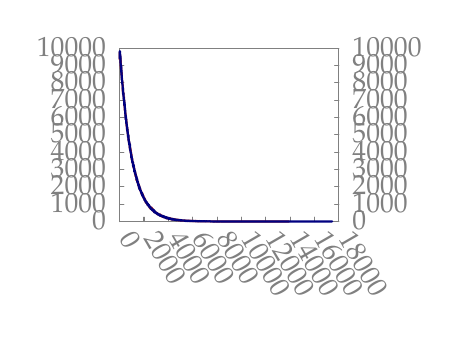
\begin{tikzpicture}[gnuplot, scale=0.3]
%% generated with GNUPLOT 5.2p2 (Lua 5.3; terminal rev. 99, script rev. 102)
%% wo 11 jul 2018 09:51:59 CEST
\path (0.000,0.000) rectangle (12.500,8.750);
\gpcolor{rgb color={0.502,0.502,0.502}}
\gpsetlinetype{gp lt border}
\gpsetdashtype{gp dt solid}
\gpsetlinewidth{1.00}
\draw[gp path] (1.380,1.104)--(1.560,1.104);
\node[gp node right] at (1.196,1.104) {$0$};
\draw[gp path] (1.380,1.838)--(1.560,1.838);
\node[gp node right] at (1.196,1.838) {$1000$};
\draw[gp path] (1.380,2.571)--(1.560,2.571);
\node[gp node right] at (1.196,2.571) {$2000$};
\draw[gp path] (1.380,3.305)--(1.560,3.305);
\node[gp node right] at (1.196,3.305) {$3000$};
\draw[gp path] (1.380,4.039)--(1.560,4.039);
\node[gp node right] at (1.196,4.039) {$4000$};
\draw[gp path] (1.380,4.773)--(1.560,4.773);
\node[gp node right] at (1.196,4.773) {$5000$};
\draw[gp path] (1.380,5.506)--(1.560,5.506);
\node[gp node right] at (1.196,5.506) {$6000$};
\draw[gp path] (1.380,6.240)--(1.560,6.240);
\node[gp node right] at (1.196,6.240) {$7000$};
\draw[gp path] (1.380,6.974)--(1.560,6.974);
\node[gp node right] at (1.196,6.974) {$8000$};
\draw[gp path] (1.380,7.707)--(1.560,7.707);
\node[gp node right] at (1.196,7.707) {$9000$};
\draw[gp path] (1.380,8.441)--(1.560,8.441);
\node[gp node right] at (1.196,8.441) {$10000$};
\draw[gp path] (1.380,1.104)--(1.380,1.284);
\node[gp node left,rotate=-60] at (1.380,0.920) {$0$};
\draw[gp path] (2.411,1.104)--(2.411,1.284);
\node[gp node left,rotate=-60] at (2.411,0.920) {$2000$};
\draw[gp path] (3.442,1.104)--(3.442,1.284);
\node[gp node left,rotate=-60] at (3.442,0.920) {$4000$};
\draw[gp path] (4.473,1.104)--(4.473,1.284);
\node[gp node left,rotate=-60] at (4.473,0.920) {$6000$};
\draw[gp path] (5.504,1.104)--(5.504,1.284);
\node[gp node left,rotate=-60] at (5.504,0.920) {$8000$};
\draw[gp path] (6.535,1.104)--(6.535,1.284);
\node[gp node left,rotate=-60] at (6.535,0.920) {$10000$};
\draw[gp path] (7.566,1.104)--(7.566,1.284);
\node[gp node left,rotate=-60] at (7.566,0.920) {$12000$};
\draw[gp path] (8.597,1.104)--(8.597,1.284);
\node[gp node left,rotate=-60] at (8.597,0.920) {$14000$};
\draw[gp path] (9.628,1.104)--(9.628,1.284);
\node[gp node left,rotate=-60] at (9.628,0.920) {$16000$};
\draw[gp path] (10.659,1.104)--(10.659,1.284);
\node[gp node left,rotate=-60] at (10.659,0.920) {$18000$};
\draw[gp path] (10.659,1.104)--(10.479,1.104);
\node[gp node left] at (10.843,1.104) {$0$};
\draw[gp path] (10.659,1.838)--(10.479,1.838);
\node[gp node left] at (10.843,1.838) {$1000$};
\draw[gp path] (10.659,2.571)--(10.479,2.571);
\node[gp node left] at (10.843,2.571) {$2000$};
\draw[gp path] (10.659,3.305)--(10.479,3.305);
\node[gp node left] at (10.843,3.305) {$3000$};
\draw[gp path] (10.659,4.039)--(10.479,4.039);
\node[gp node left] at (10.843,4.039) {$4000$};
\draw[gp path] (10.659,4.773)--(10.479,4.773);
\node[gp node left] at (10.843,4.773) {$5000$};
\draw[gp path] (10.659,5.506)--(10.479,5.506);
\node[gp node left] at (10.843,5.506) {$6000$};
\draw[gp path] (10.659,6.240)--(10.479,6.240);
\node[gp node left] at (10.843,6.240) {$7000$};
\draw[gp path] (10.659,6.974)--(10.479,6.974);
\node[gp node left] at (10.843,6.974) {$8000$};
\draw[gp path] (10.659,7.707)--(10.479,7.707);
\node[gp node left] at (10.843,7.707) {$9000$};
\draw[gp path] (10.659,8.441)--(10.479,8.441);
\node[gp node left] at (10.843,8.441) {$10000$};
\draw[gp path] (1.380,8.441)--(1.380,1.104)--(10.659,1.104)--(10.659,8.441)--cycle;
\gpcolor{rgb color={0.647,0.165,0.165}}
\gpsetlinewidth{2.00}
\draw[gp path] (1.380,7.960)--(1.385,8.266)--(1.390,8.153)--(1.395,8.153)--(1.401,8.117)%
  --(1.406,7.958)--(1.411,8.037)--(1.416,7.808)--(1.421,7.974)--(1.426,7.693)--(1.432,7.613)%
  --(1.437,7.732)--(1.442,7.513)--(1.447,7.627)--(1.452,7.431)--(1.457,7.397)--(1.462,7.306)%
  --(1.468,7.404)--(1.473,7.184)--(1.478,7.163)--(1.483,7.134)--(1.488,6.982)--(1.493,7.001)%
  --(1.499,6.933)--(1.504,6.939)--(1.509,6.811)--(1.514,6.625)--(1.519,6.734)--(1.524,6.495)%
  --(1.529,6.582)--(1.535,6.497)--(1.540,6.532)--(1.545,6.526)--(1.550,6.342)--(1.555,6.283)%
  --(1.560,6.387)--(1.566,6.209)--(1.571,6.217)--(1.576,6.004)--(1.581,6.054)--(1.586,6.016)%
  --(1.591,6.024)--(1.597,5.828)--(1.602,5.882)--(1.607,5.860)--(1.612,5.745)--(1.617,5.682)%
  --(1.622,5.700)--(1.627,5.654)--(1.633,5.572)--(1.638,5.550)--(1.643,5.436)--(1.648,5.446)%
  --(1.653,5.410)--(1.658,5.443)--(1.664,5.366)--(1.669,5.298)--(1.674,5.180)--(1.679,5.157)%
  --(1.684,5.145)--(1.689,4.979)--(1.694,5.100)--(1.700,4.994)--(1.705,5.074)--(1.710,4.936)%
  --(1.715,5.007)--(1.720,4.804)--(1.725,4.850)--(1.731,4.737)--(1.736,4.793)--(1.741,4.754)%
  --(1.746,4.734)--(1.751,4.616)--(1.756,4.615)--(1.761,4.509)--(1.767,4.581)--(1.772,4.488)%
  --(1.777,4.519)--(1.782,4.410)--(1.787,4.439)--(1.792,4.378)--(1.798,4.376)--(1.803,4.377)%
  --(1.808,4.312)--(1.813,4.191)--(1.818,4.158)--(1.823,4.234)--(1.828,4.212)--(1.834,4.165)%
  --(1.839,4.111)--(1.844,4.177)--(1.849,4.018)--(1.854,4.078)--(1.859,3.950)--(1.865,3.979)%
  --(1.870,3.886)--(1.875,3.957)--(1.880,3.945)--(1.885,3.827)--(1.890,3.706)--(1.896,3.803)%
  --(1.901,3.725)--(1.906,3.766)--(1.911,3.749)--(1.916,3.684)--(1.921,3.637)--(1.926,3.607)%
  --(1.932,3.624)--(1.937,3.557)--(1.942,3.599)--(1.947,3.558)--(1.952,3.524)--(1.957,3.448)%
  --(1.963,3.393)--(1.968,3.411)--(1.973,3.413)--(1.978,3.365)--(1.983,3.434)--(1.988,3.356)%
  --(1.993,3.320)--(1.999,3.332)--(2.004,3.296)--(2.009,3.276)--(2.014,3.271)--(2.019,3.230)%
  --(2.024,3.214)--(2.030,3.178)--(2.035,3.180)--(2.040,3.090)--(2.045,3.161)--(2.050,3.117)%
  --(2.055,3.012)--(2.060,3.096)--(2.066,3.075)--(2.071,3.007)--(2.076,2.987)--(2.081,3.017)%
  --(2.086,2.995)--(2.091,2.838)--(2.097,2.914)--(2.102,2.916)--(2.107,2.861)--(2.112,2.862)%
  --(2.117,2.848)--(2.122,2.833)--(2.127,2.847)--(2.133,2.750)--(2.138,2.778)--(2.143,2.792)%
  --(2.148,2.747)--(2.153,2.720)--(2.158,2.778)--(2.164,2.725)--(2.169,2.683)--(2.174,2.624)%
  --(2.179,2.644)--(2.184,2.660)--(2.189,2.654)--(2.194,2.573)--(2.200,2.568)--(2.205,2.615)%
  --(2.210,2.609)--(2.215,2.582)--(2.220,2.477)--(2.225,2.520)--(2.231,2.530)--(2.236,2.522)%
  --(2.241,2.496)--(2.246,2.471)--(2.251,2.425)--(2.256,2.480)--(2.262,2.395)--(2.267,2.437)%
  --(2.272,2.390)--(2.277,2.394)--(2.282,2.356)--(2.287,2.340)--(2.292,2.359)--(2.298,2.326)%
  --(2.303,2.293)--(2.308,2.273)--(2.313,2.275)--(2.318,2.302)--(2.323,2.263)--(2.329,2.326)%
  --(2.334,2.276)--(2.339,2.208)--(2.344,2.263)--(2.349,2.286)--(2.354,2.202)--(2.359,2.180)%
  --(2.365,2.208)--(2.370,2.167)--(2.375,2.187)--(2.380,2.152)--(2.385,2.199)--(2.390,2.103)%
  --(2.396,2.125)--(2.401,2.118)--(2.406,2.083)--(2.411,2.117)--(2.416,2.065)--(2.421,2.111)%
  --(2.426,2.052)--(2.432,2.021)--(2.437,2.093)--(2.442,2.013)--(2.447,2.017)--(2.452,2.031)%
  --(2.457,1.991)--(2.463,1.998)--(2.468,1.982)--(2.473,1.937)--(2.478,1.982)--(2.483,1.896)%
  --(2.488,1.937)--(2.493,1.941)--(2.499,1.902)--(2.504,1.935)--(2.509,1.921)--(2.514,1.880)%
  --(2.519,1.913)--(2.524,1.866)--(2.530,1.919)--(2.535,1.860)--(2.540,1.860)--(2.545,1.830)%
  --(2.550,1.847)--(2.555,1.860)--(2.560,1.818)--(2.566,1.801)--(2.571,1.822)--(2.576,1.800)%
  --(2.581,1.802)--(2.586,1.824)--(2.591,1.805)--(2.597,1.789)--(2.602,1.805)--(2.607,1.754)%
  --(2.612,1.763)--(2.617,1.764)--(2.622,1.797)--(2.628,1.753)--(2.633,1.765)--(2.638,1.758)%
  --(2.643,1.733)--(2.648,1.712)--(2.653,1.707)--(2.658,1.693)--(2.664,1.702)--(2.669,1.693)%
  --(2.674,1.712)--(2.679,1.637)--(2.684,1.685)--(2.689,1.642)--(2.695,1.677)--(2.700,1.670)%
  --(2.705,1.643)--(2.710,1.673)--(2.715,1.652)--(2.720,1.656)--(2.725,1.652)--(2.731,1.672)%
  --(2.736,1.692)--(2.741,1.643)--(2.746,1.603)--(2.751,1.623)--(2.756,1.611)--(2.762,1.630)%
  --(2.767,1.582)--(2.772,1.613)--(2.777,1.560)--(2.782,1.600)--(2.787,1.616)--(2.792,1.626)%
  --(2.798,1.570)--(2.803,1.565)--(2.808,1.543)--(2.813,1.538)--(2.818,1.557)--(2.823,1.568)%
  --(2.829,1.524)--(2.834,1.533)--(2.839,1.524)--(2.844,1.534)--(2.849,1.550)--(2.854,1.512)%
  --(2.859,1.513)--(2.865,1.513)--(2.870,1.517)--(2.875,1.501)--(2.880,1.506)--(2.885,1.498)%
  --(2.890,1.477)--(2.896,1.489)--(2.901,1.483)--(2.906,1.475)--(2.911,1.480)--(2.916,1.494)%
  --(2.921,1.475)--(2.927,1.477)--(2.932,1.443)--(2.937,1.479)--(2.942,1.472)--(2.947,1.461)%
  --(2.952,1.437)--(2.957,1.449)--(2.963,1.436)--(2.968,1.450)--(2.973,1.418)--(2.978,1.420)%
  --(2.983,1.453)--(2.988,1.425)--(2.994,1.416)--(2.999,1.417)--(3.004,1.411)--(3.009,1.421)%
  --(3.014,1.422)--(3.019,1.395)--(3.024,1.390)--(3.030,1.403)--(3.035,1.400)--(3.040,1.408)%
  --(3.045,1.397)--(3.050,1.381)--(3.055,1.375)--(3.061,1.375)--(3.066,1.384)--(3.071,1.373)%
  --(3.076,1.393)--(3.081,1.386)--(3.086,1.378)--(3.091,1.408)--(3.097,1.367)--(3.102,1.397)%
  --(3.107,1.364)--(3.112,1.362)--(3.117,1.342)--(3.122,1.345)--(3.128,1.340)--(3.133,1.350)%
  --(3.138,1.324)--(3.143,1.330)--(3.148,1.319)--(3.153,1.341)--(3.158,1.358)--(3.164,1.340)%
  --(3.169,1.324)--(3.174,1.307)--(3.179,1.326)--(3.184,1.318)--(3.189,1.326)--(3.195,1.322)%
  --(3.200,1.304)--(3.205,1.314)--(3.210,1.304)--(3.215,1.315)--(3.220,1.309)--(3.225,1.291)%
  --(3.231,1.298)--(3.236,1.312)--(3.241,1.293)--(3.246,1.290)--(3.251,1.283)--(3.256,1.307)%
  --(3.262,1.305)--(3.267,1.299)--(3.272,1.282)--(3.277,1.300)--(3.282,1.306)--(3.287,1.280)%
  --(3.293,1.291)--(3.298,1.268)--(3.303,1.265)--(3.308,1.266)--(3.313,1.279)--(3.318,1.262)%
  --(3.323,1.283)--(3.329,1.288)--(3.334,1.287)--(3.339,1.260)--(3.344,1.252)--(3.349,1.264)%
  --(3.354,1.256)--(3.360,1.243)--(3.365,1.249)--(3.370,1.261)--(3.375,1.254)--(3.380,1.271)%
  --(3.385,1.245)--(3.390,1.232)--(3.396,1.262)--(3.401,1.255)--(3.406,1.257)--(3.411,1.249)%
  --(3.416,1.251)--(3.421,1.246)--(3.427,1.240)--(3.432,1.246)--(3.437,1.224)--(3.442,1.239)%
  --(3.447,1.239)--(3.452,1.231)--(3.457,1.240)--(3.463,1.227)--(3.468,1.213)--(3.473,1.221)%
  --(3.478,1.243)--(3.483,1.230)--(3.488,1.216)--(3.494,1.222)--(3.499,1.218)--(3.504,1.253)%
  --(3.509,1.203)--(3.514,1.239)--(3.519,1.224)--(3.524,1.222)--(3.530,1.228)--(3.535,1.213)%
  --(3.540,1.202)--(3.545,1.198)--(3.550,1.196)--(3.555,1.208)--(3.561,1.229)--(3.566,1.222)%
  --(3.571,1.197)--(3.576,1.209)--(3.581,1.207)--(3.586,1.208)--(3.591,1.199)--(3.597,1.201)%
  --(3.602,1.199)--(3.607,1.183)--(3.612,1.198)--(3.617,1.211)--(3.622,1.188)--(3.628,1.188)%
  --(3.633,1.196)--(3.638,1.196)--(3.643,1.201)--(3.648,1.184)--(3.653,1.211)--(3.659,1.191)%
  --(3.664,1.202)--(3.669,1.188)--(3.674,1.189)--(3.679,1.194)--(3.684,1.189)--(3.689,1.205)%
  --(3.695,1.184)--(3.700,1.189)--(3.705,1.196)--(3.710,1.183)--(3.715,1.180)--(3.720,1.188)%
  --(3.726,1.176)--(3.731,1.176)--(3.736,1.177)--(3.741,1.171)--(3.746,1.173)--(3.751,1.168)%
  --(3.756,1.169)--(3.762,1.185)--(3.767,1.168)--(3.772,1.180)--(3.777,1.172)--(3.782,1.168)%
  --(3.787,1.181)--(3.793,1.174)--(3.798,1.158)--(3.803,1.158)--(3.808,1.179)--(3.813,1.176)%
  --(3.818,1.167)--(3.823,1.163)--(3.829,1.174)--(3.834,1.168)--(3.839,1.166)--(3.844,1.178)%
  --(3.849,1.173)--(3.854,1.158)--(3.860,1.169)--(3.865,1.159)--(3.870,1.163)--(3.875,1.180)%
  --(3.880,1.169)--(3.885,1.152)--(3.890,1.157)--(3.896,1.164)--(3.901,1.152)--(3.906,1.155)%
  --(3.911,1.150)--(3.916,1.155)--(3.921,1.156)--(3.927,1.154)--(3.932,1.147)--(3.937,1.155)%
  --(3.942,1.156)--(3.947,1.161)--(3.952,1.148)--(3.958,1.156)--(3.963,1.156)--(3.968,1.155)%
  --(3.973,1.147)--(3.978,1.144)--(3.983,1.155)--(3.988,1.158)--(3.994,1.149)--(3.999,1.142)%
  --(4.004,1.146)--(4.009,1.142)--(4.014,1.154)--(4.019,1.151)--(4.025,1.147)--(4.030,1.147)%
  --(4.035,1.138)--(4.040,1.141)--(4.045,1.141)--(4.050,1.144)--(4.055,1.142)--(4.061,1.145)%
  --(4.066,1.141)--(4.071,1.147)--(4.076,1.141)--(4.081,1.141)--(4.086,1.139)--(4.092,1.147)%
  --(4.097,1.144)--(4.102,1.143)--(4.107,1.139)--(4.112,1.133)--(4.117,1.130)--(4.122,1.138)%
  --(4.128,1.136)--(4.133,1.133)--(4.138,1.141)--(4.143,1.145)--(4.148,1.136)--(4.153,1.132)%
  --(4.159,1.130)--(4.164,1.144)--(4.169,1.126)--(4.174,1.127)--(4.179,1.127)--(4.184,1.127)%
  --(4.189,1.136)--(4.195,1.134)--(4.200,1.139)--(4.205,1.138)--(4.210,1.130)--(4.215,1.133)%
  --(4.220,1.131)--(4.226,1.136)--(4.231,1.130)--(4.236,1.128)--(4.241,1.126)--(4.246,1.133)%
  --(4.251,1.133)--(4.256,1.123)--(4.262,1.131)--(4.267,1.129)--(4.272,1.133)--(4.277,1.136)%
  --(4.282,1.127)--(4.287,1.125)--(4.293,1.130)--(4.298,1.126)--(4.303,1.137)--(4.308,1.135)%
  --(4.313,1.128)--(4.318,1.135)--(4.324,1.127)--(4.329,1.129)--(4.334,1.126)--(4.339,1.130)%
  --(4.344,1.139)--(4.349,1.123)--(4.354,1.126)--(4.360,1.130)--(4.365,1.133)--(4.370,1.126)%
  --(4.375,1.125)--(4.380,1.121)--(4.385,1.134)--(4.391,1.125)--(4.396,1.128)--(4.401,1.122)%
  --(4.406,1.119)--(4.411,1.118)--(4.416,1.120)--(4.421,1.121)--(4.427,1.122)--(4.432,1.120)%
  --(4.437,1.123)--(4.442,1.122)--(4.447,1.127)--(4.452,1.120)--(4.458,1.125)--(4.463,1.116)%
  --(4.468,1.122)--(4.473,1.119)--(4.478,1.125)--(4.483,1.123)--(4.488,1.116)--(4.494,1.129)%
  --(4.499,1.119)--(4.504,1.119)--(4.509,1.119)--(4.514,1.121)--(4.519,1.130)--(4.525,1.124)%
  --(4.530,1.119)--(4.535,1.122)--(4.540,1.125)--(4.545,1.121)--(4.550,1.117)--(4.555,1.123)%
  --(4.561,1.116)--(4.566,1.123)--(4.571,1.115)--(4.576,1.125)--(4.581,1.114)--(4.586,1.119)%
  --(4.592,1.127)--(4.597,1.122)--(4.602,1.120)--(4.607,1.119)--(4.612,1.119)--(4.617,1.119)%
  --(4.622,1.125)--(4.628,1.114)--(4.633,1.114)--(4.638,1.121)--(4.643,1.124)--(4.648,1.116)%
  --(4.653,1.119)--(4.659,1.121)--(4.664,1.112)--(4.669,1.123)--(4.674,1.118)--(4.679,1.119)%
  --(4.684,1.119)--(4.690,1.116)--(4.695,1.114)--(4.700,1.119)--(4.705,1.118)--(4.710,1.114)%
  --(4.715,1.119)--(4.720,1.110)--(4.726,1.120)--(4.731,1.108)--(4.736,1.115)--(4.741,1.117)%
  --(4.746,1.117)--(4.751,1.118)--(4.757,1.112)--(4.762,1.121)--(4.767,1.114)--(4.772,1.114)%
  --(4.777,1.119)--(4.782,1.113)--(4.787,1.115)--(4.793,1.114)--(4.798,1.114)--(4.803,1.115)%
  --(4.808,1.111)--(4.813,1.114)--(4.818,1.111)--(4.824,1.117)--(4.829,1.111)--(4.834,1.110)%
  --(4.839,1.114)--(4.844,1.114)--(4.849,1.113)--(4.854,1.116)--(4.860,1.111)--(4.865,1.112)%
  --(4.870,1.112)--(4.875,1.112)--(4.880,1.111)--(4.885,1.115)--(4.891,1.114)--(4.896,1.114)%
  --(4.901,1.113)--(4.906,1.112)--(4.911,1.114)--(4.916,1.112)--(4.921,1.112)--(4.927,1.114)%
  --(4.932,1.115)--(4.937,1.111)--(4.942,1.114)--(4.947,1.111)--(4.952,1.111)--(4.958,1.109)%
  --(4.963,1.112)--(4.968,1.114)--(4.973,1.111)--(4.978,1.111)--(4.983,1.112)--(4.989,1.111)%
  --(4.994,1.111)--(4.999,1.108)--(5.004,1.108)--(5.009,1.115)--(5.014,1.109)--(5.019,1.111)%
  --(5.025,1.111)--(5.030,1.113)--(5.035,1.111)--(5.040,1.110)--(5.045,1.114)--(5.050,1.109)%
  --(5.056,1.108)--(5.061,1.108)--(5.066,1.108)--(5.071,1.109)--(5.076,1.108)--(5.081,1.109)%
  --(5.086,1.111)--(5.092,1.109)--(5.097,1.110)--(5.102,1.108)--(5.107,1.107)--(5.112,1.110)%
  --(5.117,1.110)--(5.123,1.108)--(5.128,1.109)--(5.133,1.111)--(5.138,1.108)--(5.143,1.108)%
  --(5.148,1.111)--(5.153,1.108)--(5.159,1.112)--(5.164,1.109)--(5.169,1.108)--(5.174,1.106)%
  --(5.179,1.112)--(5.184,1.108)--(5.190,1.109)--(5.195,1.107)--(5.200,1.109)--(5.205,1.108)%
  --(5.210,1.111)--(5.215,1.105)--(5.220,1.108)--(5.226,1.105)--(5.231,1.107)--(5.236,1.108)%
  --(5.241,1.108)--(5.246,1.111)--(5.251,1.107)--(5.257,1.106)--(5.262,1.108)--(5.267,1.108)%
  --(5.272,1.107)--(5.277,1.108)--(5.282,1.108)--(5.287,1.108)--(5.293,1.107)--(5.298,1.105)%
  --(5.303,1.108)--(5.308,1.108)--(5.313,1.108)--(5.318,1.106)--(5.324,1.108)--(5.329,1.107)%
  --(5.334,1.109)--(5.339,1.107)--(5.344,1.108)--(5.349,1.106)--(5.355,1.105)--(5.360,1.105)%
  --(5.365,1.107)--(5.370,1.106)--(5.375,1.108)--(5.380,1.108)--(5.385,1.105)--(5.391,1.106)%
  --(5.396,1.108)--(5.401,1.105)--(5.406,1.108)--(5.411,1.106)--(5.416,1.107)--(5.422,1.105)%
  --(5.427,1.107)--(5.432,1.107)--(5.437,1.107)--(5.442,1.105)--(5.447,1.106)--(5.452,1.106)%
  --(5.458,1.106)--(5.463,1.107)--(5.468,1.108)--(5.473,1.105)--(5.478,1.108)--(5.483,1.106)%
  --(5.489,1.107)--(5.494,1.107)--(5.499,1.105)--(5.504,1.105)--(5.509,1.106)--(5.514,1.105)%
  --(5.519,1.105)--(5.525,1.111)--(5.530,1.107)--(5.535,1.108)--(5.540,1.107)--(5.545,1.105)%
  --(5.550,1.105)--(5.556,1.106)--(5.561,1.105)--(5.566,1.105)--(5.571,1.108)--(5.576,1.105)%
  --(5.581,1.108)--(5.586,1.105)--(5.592,1.108)--(5.597,1.105)--(5.602,1.105)--(5.607,1.105)%
  --(5.612,1.108)--(5.617,1.105)--(5.623,1.108)--(5.628,1.107)--(5.633,1.106)--(5.638,1.105)%
  --(5.648,1.105)--(5.653,1.106)--(5.659,1.106)--(5.664,1.105)--(5.669,1.105)--(5.679,1.108)%
  --(5.684,1.105)--(5.695,1.105)--(5.700,1.105)--(5.705,1.105)--(5.710,1.105)--(5.715,1.106)%
  --(5.721,1.105)--(5.726,1.106)--(5.731,1.105)--(5.736,1.105)--(5.741,1.105)--(5.746,1.105)%
  --(5.751,1.105)--(5.757,1.105)--(5.762,1.105)--(5.767,1.105)--(5.772,1.106)--(5.782,1.106)%
  --(5.788,1.105)--(5.793,1.105)--(5.803,1.106)--(5.808,1.105)--(5.813,1.106)--(5.818,1.105)%
  --(5.824,1.105)--(5.829,1.105)--(5.834,1.106)--(5.849,1.105)--(5.855,1.105)--(5.860,1.105)%
  --(5.870,1.105)--(5.875,1.107)--(5.885,1.105)--(5.891,1.105)--(5.896,1.105)--(5.901,1.105)%
  --(5.906,1.105)--(5.911,1.107)--(5.916,1.106)--(5.922,1.106)--(5.927,1.105)--(5.937,1.105)%
  --(5.942,1.105)--(5.963,1.106)--(5.968,1.105)--(5.973,1.106)--(5.978,1.105)--(5.983,1.105)%
  --(5.994,1.105)--(6.004,1.105)--(6.009,1.105)--(6.020,1.105)--(6.025,1.105)--(6.030,1.105)%
  --(6.035,1.107)--(6.040,1.105)--(6.056,1.106)--(6.061,1.105)--(6.066,1.105)--(6.071,1.105)%
  --(6.076,1.105)--(6.087,1.105)--(6.097,1.105)--(6.107,1.106)--(6.117,1.105)--(6.128,1.108)%
  --(6.133,1.105)--(6.143,1.105)--(6.154,1.105)--(6.159,1.105)--(6.164,1.105)--(6.169,1.105)%
  --(6.174,1.105)--(6.179,1.105)--(6.190,1.106)--(6.195,1.105)--(6.205,1.105)--(6.210,1.106)%
  --(6.221,1.105)--(6.241,1.105)--(6.246,1.105)--(6.251,1.105)--(6.257,1.105)--(6.282,1.105)%
  --(6.293,1.105)--(6.298,1.105)--(6.313,1.105)--(6.324,1.105)--(6.339,1.105)--(6.344,1.105)%
  --(6.365,1.105)--(6.380,1.105)--(6.391,1.105)--(6.427,1.105)--(6.432,1.105)--(6.447,1.105)%
  --(6.463,1.105)--(6.468,1.105)--(6.473,1.105)--(6.509,1.105)--(6.520,1.105)--(6.530,1.105)%
  --(6.535,1.105)--(6.540,1.105)--(6.545,1.105)--(6.550,1.105)--(6.561,1.105)--(6.566,1.105)%
  --(6.576,1.105)--(6.581,1.105)--(6.602,1.105)--(6.617,1.105)--(6.659,1.105)--(6.700,1.105)%
  --(6.710,1.105)--(6.715,1.105)--(6.731,1.105)--(6.736,1.105)--(6.746,1.105)--(6.752,1.105)%
  --(6.757,1.105)--(6.762,1.105)--(6.767,1.105)--(6.788,1.105)--(6.849,1.105)--(6.886,1.105)%
  --(6.896,1.105)--(6.916,1.105)--(6.947,1.105)--(7.004,1.105)--(7.020,1.105)--(7.045,1.105)%
  --(7.050,1.105)--(7.066,1.105)--(7.076,1.105)--(7.102,1.105)--(7.118,1.105)--(7.123,1.105)%
  --(7.133,1.105)--(7.169,1.105)--(7.179,1.105)--(7.185,1.105)--(7.221,1.105)--(7.329,1.105)%
  --(7.339,1.105)--(7.473,1.105)--(7.484,1.105)--(7.551,1.105)--(7.618,1.105)--(7.798,1.105)%
  --(7.803,1.105)--(7.901,1.105)--(8.246,1.105)--(8.551,1.105);
\gpcolor{rgb color={0.000,0.000,0.502}}
\draw[gp path] (1.380,8.008)--(1.385,8.286)--(1.390,8.318)--(1.395,8.170)--(1.401,8.173)%
  --(1.406,8.015)--(1.411,8.111)--(1.416,7.845)--(1.421,7.801)--(1.426,7.714)--(1.432,7.674)%
  --(1.437,7.558)--(1.442,7.720)--(1.447,7.522)--(1.452,7.423)--(1.457,7.507)--(1.462,7.293)%
  --(1.468,7.296)--(1.473,7.101)--(1.478,7.073)--(1.483,7.054)--(1.488,7.056)--(1.493,6.947)%
  --(1.499,6.872)--(1.504,6.909)--(1.509,6.704)--(1.514,6.777)--(1.519,6.760)--(1.524,6.621)%
  --(1.529,6.498)--(1.535,6.486)--(1.540,6.541)--(1.545,6.423)--(1.550,6.349)--(1.555,6.296)%
  --(1.560,6.266)--(1.566,6.205)--(1.571,6.253)--(1.576,6.048)--(1.581,6.155)--(1.586,6.012)%
  --(1.591,6.092)--(1.597,5.958)--(1.602,5.916)--(1.607,5.807)--(1.612,5.814)--(1.617,5.800)%
  --(1.622,5.640)--(1.627,5.492)--(1.633,5.624)--(1.638,5.408)--(1.643,5.521)--(1.648,5.527)%
  --(1.653,5.498)--(1.658,5.366)--(1.664,5.252)--(1.669,5.303)--(1.674,5.255)--(1.679,5.200)%
  --(1.684,5.148)--(1.689,5.158)--(1.694,5.073)--(1.700,4.934)--(1.705,5.078)--(1.710,4.965)%
  --(1.715,4.877)--(1.720,4.899)--(1.725,4.830)--(1.731,4.809)--(1.736,4.671)--(1.741,4.767)%
  --(1.746,4.675)--(1.751,4.742)--(1.756,4.543)--(1.761,4.568)--(1.767,4.569)--(1.772,4.423)%
  --(1.777,4.485)--(1.782,4.480)--(1.787,4.352)--(1.792,4.434)--(1.798,4.343)--(1.803,4.333)%
  --(1.808,4.232)--(1.813,4.371)--(1.818,4.318)--(1.823,4.145)--(1.828,4.180)--(1.834,4.087)%
  --(1.839,4.097)--(1.844,4.062)--(1.849,4.019)--(1.854,4.019)--(1.859,4.018)--(1.865,3.973)%
  --(1.870,3.817)--(1.875,3.905)--(1.880,3.874)--(1.885,3.820)--(1.890,3.844)--(1.896,3.754)%
  --(1.901,3.739)--(1.906,3.772)--(1.911,3.681)--(1.916,3.611)--(1.921,3.624)--(1.926,3.602)%
  --(1.932,3.578)--(1.937,3.624)--(1.942,3.610)--(1.947,3.467)--(1.952,3.491)--(1.957,3.442)%
  --(1.963,3.425)--(1.968,3.491)--(1.973,3.498)--(1.978,3.389)--(1.983,3.376)--(1.988,3.362)%
  --(1.993,3.376)--(1.999,3.212)--(2.004,3.284)--(2.009,3.265)--(2.014,3.254)--(2.019,3.268)%
  --(2.024,3.204)--(2.030,3.150)--(2.035,3.123)--(2.040,3.212)--(2.045,3.103)--(2.050,3.072)%
  --(2.055,3.108)--(2.060,3.063)--(2.066,3.062)--(2.071,3.048)--(2.076,2.995)--(2.081,2.963)%
  --(2.086,3.012)--(2.091,2.962)--(2.097,2.875)--(2.102,2.923)--(2.107,2.943)--(2.112,2.927)%
  --(2.117,2.896)--(2.122,2.890)--(2.127,2.779)--(2.133,2.794)--(2.138,2.781)--(2.143,2.803)%
  --(2.148,2.748)--(2.153,2.728)--(2.158,2.720)--(2.164,2.651)--(2.169,2.699)--(2.174,2.687)%
  --(2.179,2.618)--(2.184,2.612)--(2.189,2.660)--(2.194,2.625)--(2.200,2.532)--(2.205,2.525)%
  --(2.210,2.597)--(2.215,2.568)--(2.220,2.555)--(2.225,2.456)--(2.231,2.502)--(2.236,2.458)%
  --(2.241,2.522)--(2.246,2.431)--(2.251,2.447)--(2.256,2.404)--(2.262,2.418)--(2.267,2.427)%
  --(2.272,2.409)--(2.277,2.392)--(2.282,2.358)--(2.287,2.368)--(2.292,2.331)--(2.298,2.355)%
  --(2.303,2.311)--(2.308,2.285)--(2.313,2.336)--(2.318,2.294)--(2.323,2.246)--(2.329,2.308)%
  --(2.334,2.218)--(2.339,2.190)--(2.344,2.212)--(2.349,2.236)--(2.354,2.224)--(2.359,2.246)%
  --(2.365,2.180)--(2.370,2.172)--(2.375,2.154)--(2.380,2.147)--(2.385,2.147)--(2.390,2.104)%
  --(2.396,2.104)--(2.401,2.114)--(2.406,2.119)--(2.411,2.105)--(2.416,2.077)--(2.421,2.073)%
  --(2.426,2.056)--(2.432,2.008)--(2.437,2.049)--(2.442,2.048)--(2.447,2.017)--(2.452,2.004)%
  --(2.457,1.994)--(2.463,1.995)--(2.468,1.958)--(2.473,2.006)--(2.478,1.979)--(2.483,1.959)%
  --(2.488,1.958)--(2.493,1.913)--(2.499,1.948)--(2.504,1.933)--(2.509,1.922)--(2.514,1.882)%
  --(2.519,1.918)--(2.524,1.914)--(2.530,1.905)--(2.535,1.858)--(2.540,1.891)--(2.545,1.871)%
  --(2.550,1.857)--(2.555,1.882)--(2.560,1.800)--(2.566,1.859)--(2.571,1.863)--(2.576,1.843)%
  --(2.581,1.846)--(2.586,1.830)--(2.591,1.780)--(2.597,1.807)--(2.602,1.756)--(2.607,1.796)%
  --(2.612,1.804)--(2.617,1.797)--(2.622,1.764)--(2.628,1.786)--(2.633,1.753)--(2.638,1.778)%
  --(2.643,1.700)--(2.648,1.703)--(2.653,1.728)--(2.658,1.717)--(2.664,1.713)--(2.669,1.712)%
  --(2.674,1.695)--(2.679,1.723)--(2.684,1.703)--(2.689,1.672)--(2.695,1.670)--(2.700,1.655)%
  --(2.705,1.629)--(2.710,1.652)--(2.715,1.672)--(2.720,1.645)--(2.725,1.642)--(2.731,1.612)%
  --(2.736,1.634)--(2.741,1.614)--(2.746,1.621)--(2.751,1.582)--(2.756,1.597)--(2.762,1.602)%
  --(2.767,1.626)--(2.772,1.584)--(2.777,1.563)--(2.782,1.597)--(2.787,1.584)--(2.792,1.584)%
  --(2.798,1.567)--(2.803,1.596)--(2.808,1.558)--(2.813,1.563)--(2.818,1.599)--(2.823,1.565)%
  --(2.829,1.559)--(2.834,1.565)--(2.839,1.524)--(2.844,1.488)--(2.849,1.518)--(2.854,1.565)%
  --(2.859,1.498)--(2.865,1.525)--(2.870,1.524)--(2.875,1.480)--(2.880,1.496)--(2.885,1.509)%
  --(2.890,1.475)--(2.896,1.499)--(2.901,1.462)--(2.906,1.462)--(2.911,1.484)--(2.916,1.475)%
  --(2.921,1.469)--(2.927,1.477)--(2.932,1.458)--(2.937,1.450)--(2.942,1.477)--(2.947,1.450)%
  --(2.952,1.450)--(2.957,1.423)--(2.963,1.458)--(2.968,1.420)--(2.973,1.429)--(2.978,1.455)%
  --(2.983,1.408)--(2.988,1.433)--(2.994,1.401)--(2.999,1.407)--(3.004,1.437)--(3.009,1.425)%
  --(3.014,1.414)--(3.019,1.403)--(3.024,1.397)--(3.030,1.417)--(3.035,1.393)--(3.040,1.397)%
  --(3.045,1.389)--(3.050,1.366)--(3.055,1.376)--(3.061,1.375)--(3.066,1.375)--(3.071,1.364)%
  --(3.076,1.348)--(3.081,1.370)--(3.086,1.363)--(3.091,1.395)--(3.097,1.348)--(3.102,1.378)%
  --(3.107,1.350)--(3.112,1.356)--(3.117,1.372)--(3.122,1.358)--(3.128,1.348)--(3.133,1.342)%
  --(3.138,1.334)--(3.143,1.356)--(3.148,1.335)--(3.153,1.328)--(3.158,1.330)--(3.164,1.332)%
  --(3.169,1.326)--(3.174,1.351)--(3.179,1.320)--(3.184,1.341)--(3.189,1.337)--(3.195,1.329)%
  --(3.200,1.305)--(3.205,1.339)--(3.210,1.318)--(3.215,1.315)--(3.220,1.323)--(3.225,1.312)%
  --(3.231,1.337)--(3.236,1.281)--(3.241,1.309)--(3.246,1.295)--(3.251,1.301)--(3.256,1.288)%
  --(3.262,1.295)--(3.267,1.290)--(3.272,1.319)--(3.277,1.283)--(3.282,1.307)--(3.287,1.280)%
  --(3.293,1.276)--(3.298,1.287)--(3.303,1.301)--(3.308,1.273)--(3.313,1.279)--(3.318,1.265)%
  --(3.323,1.295)--(3.329,1.280)--(3.334,1.273)--(3.339,1.243)--(3.344,1.257)--(3.349,1.239)%
  --(3.354,1.270)--(3.360,1.266)--(3.365,1.246)--(3.370,1.243)--(3.375,1.286)--(3.380,1.257)%
  --(3.385,1.240)--(3.390,1.240)--(3.396,1.238)--(3.401,1.253)--(3.406,1.247)--(3.411,1.238)%
  --(3.416,1.243)--(3.421,1.240)--(3.427,1.235)--(3.432,1.241)--(3.437,1.257)--(3.442,1.240)%
  --(3.447,1.211)--(3.452,1.226)--(3.457,1.238)--(3.463,1.221)--(3.468,1.238)--(3.473,1.219)%
  --(3.478,1.215)--(3.483,1.213)--(3.488,1.221)--(3.494,1.235)--(3.499,1.241)--(3.504,1.224)%
  --(3.509,1.211)--(3.514,1.223)--(3.519,1.220)--(3.524,1.213)--(3.530,1.219)--(3.535,1.221)%
  --(3.540,1.207)--(3.545,1.224)--(3.550,1.205)--(3.555,1.200)--(3.561,1.213)--(3.566,1.216)%
  --(3.571,1.205)--(3.576,1.202)--(3.581,1.193)--(3.586,1.204)--(3.591,1.187)--(3.597,1.191)%
  --(3.602,1.222)--(3.607,1.202)--(3.612,1.189)--(3.617,1.190)--(3.622,1.198)--(3.628,1.202)%
  --(3.633,1.195)--(3.638,1.180)--(3.643,1.199)--(3.648,1.188)--(3.653,1.187)--(3.659,1.188)%
  --(3.664,1.198)--(3.669,1.188)--(3.674,1.185)--(3.679,1.178)--(3.684,1.191)--(3.689,1.178)%
  --(3.695,1.187)--(3.700,1.193)--(3.705,1.181)--(3.710,1.183)--(3.715,1.180)--(3.720,1.188)%
  --(3.726,1.166)--(3.731,1.195)--(3.736,1.167)--(3.741,1.185)--(3.746,1.172)--(3.751,1.170)%
  --(3.756,1.176)--(3.762,1.168)--(3.767,1.172)--(3.772,1.167)--(3.777,1.164)--(3.782,1.179)%
  --(3.787,1.160)--(3.793,1.169)--(3.798,1.169)--(3.803,1.160)--(3.808,1.167)--(3.813,1.180)%
  --(3.818,1.173)--(3.823,1.174)--(3.829,1.169)--(3.834,1.167)--(3.839,1.169)--(3.844,1.169)%
  --(3.849,1.163)--(3.854,1.154)--(3.860,1.168)--(3.865,1.160)--(3.870,1.160)--(3.875,1.166)%
  --(3.880,1.169)--(3.885,1.163)--(3.890,1.159)--(3.896,1.168)--(3.901,1.157)--(3.906,1.162)%
  --(3.911,1.160)--(3.916,1.158)--(3.921,1.159)--(3.927,1.164)--(3.932,1.163)--(3.937,1.152)%
  --(3.942,1.163)--(3.947,1.149)--(3.952,1.163)--(3.958,1.147)--(3.963,1.151)--(3.968,1.152)%
  --(3.973,1.157)--(3.978,1.145)--(3.983,1.152)--(3.988,1.155)--(3.994,1.144)--(3.999,1.155)%
  --(4.004,1.153)--(4.009,1.140)--(4.014,1.142)--(4.019,1.147)--(4.025,1.149)--(4.030,1.143)%
  --(4.035,1.147)--(4.040,1.141)--(4.045,1.147)--(4.050,1.149)--(4.055,1.149)--(4.061,1.149)%
  --(4.066,1.138)--(4.071,1.140)--(4.076,1.145)--(4.081,1.149)--(4.086,1.144)--(4.092,1.140)%
  --(4.097,1.142)--(4.102,1.138)--(4.107,1.141)--(4.112,1.138)--(4.117,1.154)--(4.122,1.131)%
  --(4.128,1.140)--(4.133,1.138)--(4.138,1.135)--(4.143,1.136)--(4.148,1.133)--(4.153,1.140)%
  --(4.159,1.138)--(4.164,1.138)--(4.169,1.136)--(4.174,1.127)--(4.179,1.141)--(4.184,1.136)%
  --(4.189,1.130)--(4.195,1.126)--(4.200,1.139)--(4.205,1.138)--(4.210,1.135)--(4.215,1.138)%
  --(4.220,1.124)--(4.226,1.132)--(4.231,1.127)--(4.236,1.127)--(4.241,1.127)--(4.246,1.128)%
  --(4.251,1.129)--(4.256,1.125)--(4.262,1.129)--(4.267,1.134)--(4.272,1.128)--(4.277,1.129)%
  --(4.282,1.127)--(4.287,1.138)--(4.293,1.138)--(4.298,1.128)--(4.303,1.132)--(4.308,1.125)%
  --(4.313,1.125)--(4.318,1.134)--(4.324,1.130)--(4.329,1.130)--(4.334,1.119)--(4.339,1.117)%
  --(4.344,1.126)--(4.349,1.125)--(4.354,1.125)--(4.360,1.122)--(4.365,1.130)--(4.370,1.128)%
  --(4.375,1.123)--(4.380,1.131)--(4.385,1.127)--(4.391,1.126)--(4.396,1.120)--(4.401,1.124)%
  --(4.406,1.125)--(4.411,1.131)--(4.416,1.124)--(4.421,1.121)--(4.427,1.130)--(4.432,1.125)%
  --(4.437,1.119)--(4.442,1.125)--(4.447,1.125)--(4.452,1.119)--(4.458,1.126)--(4.463,1.119)%
  --(4.468,1.121)--(4.473,1.120)--(4.478,1.127)--(4.483,1.119)--(4.488,1.125)--(4.494,1.123)%
  --(4.499,1.120)--(4.504,1.119)--(4.509,1.123)--(4.514,1.116)--(4.519,1.121)--(4.525,1.119)%
  --(4.530,1.122)--(4.535,1.124)--(4.540,1.119)--(4.545,1.117)--(4.550,1.115)--(4.555,1.120)%
  --(4.561,1.117)--(4.566,1.114)--(4.571,1.116)--(4.576,1.121)--(4.581,1.127)--(4.586,1.118)%
  --(4.592,1.116)--(4.597,1.115)--(4.602,1.122)--(4.607,1.119)--(4.612,1.116)--(4.617,1.119)%
  --(4.622,1.119)--(4.628,1.114)--(4.633,1.116)--(4.638,1.119)--(4.643,1.118)--(4.648,1.116)%
  --(4.653,1.116)--(4.659,1.116)--(4.664,1.119)--(4.669,1.122)--(4.674,1.117)--(4.679,1.111)%
  --(4.684,1.116)--(4.690,1.119)--(4.695,1.116)--(4.700,1.113)--(4.705,1.116)--(4.710,1.115)%
  --(4.715,1.114)--(4.720,1.115)--(4.726,1.118)--(4.731,1.119)--(4.736,1.116)--(4.741,1.113)%
  --(4.746,1.118)--(4.751,1.114)--(4.757,1.119)--(4.762,1.113)--(4.767,1.116)--(4.772,1.115)%
  --(4.777,1.111)--(4.782,1.118)--(4.787,1.114)--(4.793,1.117)--(4.798,1.115)--(4.803,1.110)%
  --(4.808,1.114)--(4.813,1.113)--(4.818,1.112)--(4.824,1.118)--(4.829,1.114)--(4.834,1.113)%
  --(4.839,1.113)--(4.844,1.113)--(4.849,1.112)--(4.854,1.108)--(4.860,1.110)--(4.865,1.113)%
  --(4.870,1.110)--(4.875,1.111)--(4.880,1.114)--(4.885,1.109)--(4.891,1.111)--(4.896,1.109)%
  --(4.901,1.111)--(4.906,1.113)--(4.911,1.112)--(4.916,1.111)--(4.921,1.111)--(4.927,1.112)%
  --(4.932,1.112)--(4.937,1.110)--(4.942,1.110)--(4.947,1.109)--(4.952,1.115)--(4.958,1.111)%
  --(4.963,1.114)--(4.968,1.113)--(4.973,1.108)--(4.978,1.114)--(4.983,1.111)--(4.989,1.108)%
  --(4.994,1.113)--(4.999,1.111)--(5.004,1.111)--(5.009,1.111)--(5.014,1.112)--(5.019,1.108)%
  --(5.025,1.107)--(5.030,1.110)--(5.035,1.114)--(5.040,1.109)--(5.045,1.110)--(5.050,1.110)%
  --(5.056,1.108)--(5.061,1.109)--(5.066,1.111)--(5.071,1.110)--(5.076,1.108)--(5.081,1.110)%
  --(5.086,1.109)--(5.092,1.110)--(5.097,1.114)--(5.102,1.108)--(5.107,1.108)--(5.112,1.108)%
  --(5.117,1.108)--(5.123,1.106)--(5.128,1.113)--(5.133,1.108)--(5.138,1.110)--(5.143,1.111)%
  --(5.148,1.108)--(5.153,1.108)--(5.159,1.108)--(5.164,1.105)--(5.169,1.107)--(5.174,1.109)%
  --(5.179,1.109)--(5.184,1.111)--(5.190,1.111)--(5.195,1.108)--(5.200,1.108)--(5.205,1.108)%
  --(5.210,1.107)--(5.215,1.114)--(5.220,1.108)--(5.226,1.105)--(5.231,1.107)--(5.236,1.106)%
  --(5.241,1.105)--(5.246,1.109)--(5.251,1.108)--(5.257,1.110)--(5.262,1.112)--(5.267,1.105)%
  --(5.272,1.108)--(5.277,1.107)--(5.282,1.108)--(5.287,1.106)--(5.293,1.108)--(5.298,1.106)%
  --(5.303,1.106)--(5.308,1.108)--(5.313,1.108)--(5.318,1.106)--(5.324,1.106)--(5.329,1.107)%
  --(5.334,1.108)--(5.339,1.107)--(5.344,1.105)--(5.349,1.105)--(5.355,1.108)--(5.360,1.108)%
  --(5.365,1.105)--(5.370,1.107)--(5.375,1.110)--(5.380,1.105)--(5.385,1.105)--(5.391,1.108)%
  --(5.396,1.111)--(5.401,1.108)--(5.406,1.106)--(5.411,1.108)--(5.416,1.107)--(5.422,1.106)%
  --(5.427,1.107)--(5.432,1.106)--(5.437,1.105)--(5.442,1.107)--(5.447,1.105)--(5.452,1.107)%
  --(5.458,1.109)--(5.463,1.108)--(5.468,1.106)--(5.473,1.106)--(5.478,1.105)--(5.483,1.107)%
  --(5.489,1.108)--(5.494,1.105)--(5.499,1.106)--(5.504,1.106)--(5.509,1.107)--(5.514,1.105)%
  --(5.519,1.108)--(5.525,1.107)--(5.530,1.105)--(5.535,1.105)--(5.540,1.105)--(5.545,1.105)%
  --(5.550,1.106)--(5.556,1.106)--(5.561,1.106)--(5.566,1.107)--(5.571,1.105)--(5.576,1.105)%
  --(5.581,1.106)--(5.586,1.105)--(5.592,1.105)--(5.597,1.107)--(5.602,1.107)--(5.607,1.105)%
  --(5.612,1.107)--(5.617,1.108)--(5.623,1.106)--(5.628,1.105)--(5.633,1.108)--(5.638,1.106)%
  --(5.643,1.108)--(5.653,1.108)--(5.659,1.107)--(5.664,1.108)--(5.669,1.106)--(5.674,1.105)%
  --(5.679,1.105)--(5.684,1.108)--(5.690,1.105)--(5.700,1.106)--(5.705,1.107)--(5.710,1.105)%
  --(5.715,1.106)--(5.721,1.105)--(5.726,1.106)--(5.731,1.106)--(5.736,1.105)--(5.741,1.105)%
  --(5.746,1.108)--(5.751,1.105)--(5.757,1.107)--(5.762,1.105)--(5.767,1.105)--(5.772,1.105)%
  --(5.777,1.105)--(5.782,1.105)--(5.788,1.105)--(5.793,1.107)--(5.798,1.106)--(5.803,1.105)%
  --(5.808,1.105)--(5.813,1.105)--(5.818,1.106)--(5.829,1.107)--(5.844,1.106)--(5.849,1.105)%
  --(5.855,1.105)--(5.865,1.105)--(5.870,1.106)--(5.875,1.105)--(5.880,1.105)--(5.885,1.105)%
  --(5.901,1.105)--(5.906,1.105)--(5.911,1.106)--(5.916,1.105)--(5.927,1.106)--(5.932,1.105)%
  --(5.937,1.105)--(5.942,1.105)--(5.952,1.105)--(5.963,1.105)--(5.968,1.105)--(5.973,1.105)%
  --(5.978,1.106)--(5.983,1.108)--(5.989,1.106)--(5.999,1.105)--(6.009,1.105)--(6.025,1.106)%
  --(6.030,1.107)--(6.035,1.105)--(6.045,1.105)--(6.050,1.105)--(6.061,1.105)--(6.071,1.105)%
  --(6.076,1.105)--(6.081,1.105)--(6.092,1.105)--(6.102,1.105)--(6.107,1.106)--(6.112,1.105)%
  --(6.117,1.105)--(6.123,1.105)--(6.128,1.105)--(6.133,1.105)--(6.138,1.105)--(6.148,1.105)%
  --(6.154,1.106)--(6.159,1.106)--(6.179,1.106)--(6.190,1.105)--(6.195,1.105)--(6.221,1.105)%
  --(6.226,1.105)--(6.236,1.105)--(6.246,1.105)--(6.257,1.105)--(6.262,1.105)--(6.288,1.105)%
  --(6.293,1.106)--(6.303,1.105)--(6.318,1.105)--(6.339,1.105)--(6.344,1.105)--(6.355,1.105)%
  --(6.365,1.105)--(6.375,1.105)--(6.380,1.105)--(6.386,1.105)--(6.396,1.105)--(6.416,1.106)%
  --(6.422,1.105)--(6.427,1.105)--(6.437,1.106)--(6.463,1.105)--(6.483,1.105)--(6.504,1.105)%
  --(6.509,1.107)--(6.514,1.105)--(6.525,1.105)--(6.530,1.105)--(6.535,1.105)--(6.540,1.105)%
  --(6.556,1.105)--(6.571,1.105)--(6.587,1.105)--(6.602,1.105)--(6.607,1.105)--(6.633,1.105)%
  --(6.648,1.105)--(6.659,1.105)--(6.674,1.105)--(6.684,1.105)--(6.705,1.105)--(6.788,1.105)%
  --(6.803,1.105)--(6.808,1.105)--(6.849,1.105)--(6.865,1.105)--(6.947,1.105)--(7.050,1.105)%
  --(7.066,1.105)--(7.081,1.105)--(7.112,1.105)--(7.339,1.105)--(7.344,1.105)--(7.401,1.105)%
  --(7.473,1.105)--(7.509,1.105)--(7.581,1.105)--(7.648,1.105)--(7.700,1.105)--(7.813,1.105)%
  --(7.839,1.105)--(8.154,1.105)--(8.210,1.105)--(8.257,1.105)--(8.437,1.105)--(10.375,1.105);
%% coordinates of the plot area
\gpdefrectangularnode{gp plot 1}{\pgfpoint{1.380cm}{1.104cm}}{\pgfpoint{10.659cm}{8.441cm}}
\end{tikzpicture}
%% gnuplot variables

\end{tabular}
\end{center}
\caption{\label{fig:inputselection:erlang1_1to1_randomOn}
  \texttt{Random-Improve}, 1:1 deposit:payment ratio, deposits and payments
  both drawn from an exponential distribution with scale 1000.
}
\end{figure}

\subsubsection{Erlang}

The exponential distribution results in many very small deposits and payments.
The algorithm does better on slightly more realistic distributions such as the
Erlang-$k$ distributions (for $k > 1$)\footnote{The exponential distribution
discussed in Section~\ref{sec:inputselection:erlang1_1to1_randomOn} is the
Erlang-1 case, of course.}.
Figure~\ref{fig:inputselection:erlang3_3to1_randomOn} shows the results for the
3:1 deposit:payment ratio using the Erlang-3 distribution; the results for other
ratios (including 1:1) and other values of $k$ (we additionally simulated for $k =
2$ and $k = 10$) are similar.

\begin{figure}[p]
\begin{center}
\scriptsize
\begin{tabular}{ll}
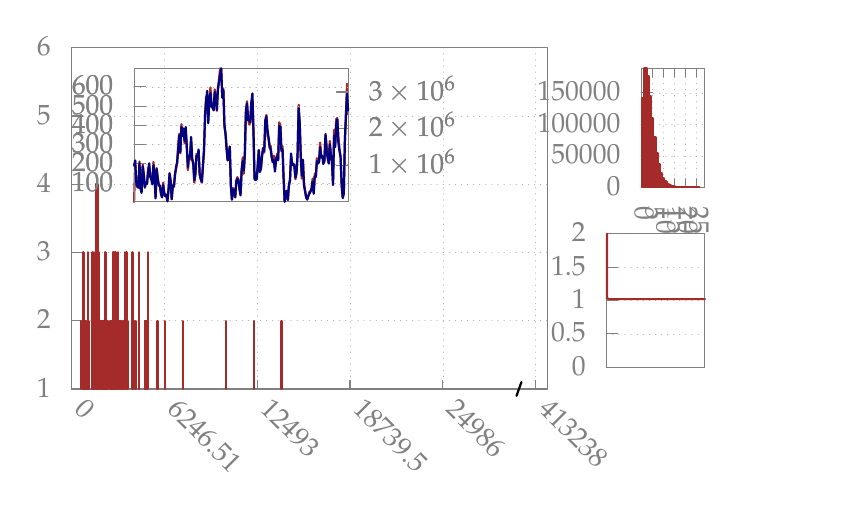
\begin{tikzpicture}[gnuplot, xscale=0.8, yscale=0.6]
%% generated with GNUPLOT 5.2p2 (Lua 5.3; terminal rev. 99, script rev. 102)
%% wo 11 jul 2018 11:27:13 CEST
\path (0.000,0.000) rectangle (12.500,8.750);
\gpcolor{color=gp lt color axes}
\gpsetlinetype{gp lt axes}
\gpsetdashtype{gp dt axes}
\gpsetlinewidth{0.50}
\draw[gp path] (0.644,1.218)--(8.197,1.218);
\gpcolor{rgb color={0.502,0.502,0.502}}
\gpsetlinetype{gp lt border}
\gpsetdashtype{gp dt solid}
\gpsetlinewidth{1.00}
\draw[gp path] (0.644,1.218)--(0.824,1.218);
\node[gp node right] at (0.460,1.218) {$1$};
\gpcolor{color=gp lt color axes}
\gpsetlinetype{gp lt axes}
\gpsetdashtype{gp dt axes}
\gpsetlinewidth{0.50}
\draw[gp path] (0.644,2.663)--(8.197,2.663);
\gpcolor{rgb color={0.502,0.502,0.502}}
\gpsetlinetype{gp lt border}
\gpsetdashtype{gp dt solid}
\gpsetlinewidth{1.00}
\draw[gp path] (0.644,2.663)--(0.824,2.663);
\node[gp node right] at (0.460,2.663) {$2$};
\gpcolor{color=gp lt color axes}
\gpsetlinetype{gp lt axes}
\gpsetdashtype{gp dt axes}
\gpsetlinewidth{0.50}
\draw[gp path] (0.644,4.107)--(8.197,4.107);
\gpcolor{rgb color={0.502,0.502,0.502}}
\gpsetlinetype{gp lt border}
\gpsetdashtype{gp dt solid}
\gpsetlinewidth{1.00}
\draw[gp path] (0.644,4.107)--(0.824,4.107);
\node[gp node right] at (0.460,4.107) {$3$};
\gpcolor{color=gp lt color axes}
\gpsetlinetype{gp lt axes}
\gpsetdashtype{gp dt axes}
\gpsetlinewidth{0.50}
\draw[gp path] (0.644,5.552)--(8.197,5.552);
\gpcolor{rgb color={0.502,0.502,0.502}}
\gpsetlinetype{gp lt border}
\gpsetdashtype{gp dt solid}
\gpsetlinewidth{1.00}
\draw[gp path] (0.644,5.552)--(0.824,5.552);
\node[gp node right] at (0.460,5.552) {$4$};
\gpcolor{color=gp lt color axes}
\gpsetlinetype{gp lt axes}
\gpsetdashtype{gp dt axes}
\gpsetlinewidth{0.50}
\draw[gp path] (0.644,6.996)--(8.197,6.996);
\gpcolor{rgb color={0.502,0.502,0.502}}
\gpsetlinetype{gp lt border}
\gpsetdashtype{gp dt solid}
\gpsetlinewidth{1.00}
\draw[gp path] (0.644,6.996)--(0.824,6.996);
\node[gp node right] at (0.460,6.996) {$5$};
\gpcolor{color=gp lt color axes}
\gpsetlinetype{gp lt axes}
\gpsetdashtype{gp dt axes}
\gpsetlinewidth{0.50}
\draw[gp path] (0.644,8.441)--(8.197,8.441);
\gpcolor{rgb color={0.502,0.502,0.502}}
\gpsetlinetype{gp lt border}
\gpsetdashtype{gp dt solid}
\gpsetlinewidth{1.00}
\draw[gp path] (0.644,8.441)--(0.824,8.441);
\node[gp node right] at (0.460,8.441) {$6$};
\gpcolor{color=gp lt color axes}
\gpsetlinetype{gp lt axes}
\gpsetdashtype{gp dt axes}
\gpsetlinewidth{0.50}
\draw[gp path] (0.644,1.218)--(0.644,8.441);
\gpcolor{rgb color={0.502,0.502,0.502}}
\gpsetlinetype{gp lt border}
\gpsetdashtype{gp dt solid}
\gpsetlinewidth{1.00}
\draw[gp path] (0.644,1.218)--(0.644,1.398);
\node[gp node left,rotate=-45] at (0.644,1.034) {$0$};
\gpcolor{color=gp lt color axes}
\gpsetlinetype{gp lt axes}
\gpsetdashtype{gp dt axes}
\gpsetlinewidth{0.50}
\draw[gp path] (2.118,1.218)--(2.118,8.441);
\gpcolor{rgb color={0.502,0.502,0.502}}
\gpsetlinetype{gp lt border}
\gpsetdashtype{gp dt solid}
\gpsetlinewidth{1.00}
\draw[gp path] (2.118,1.218)--(2.118,1.398);
\node[gp node left,rotate=-45] at (2.118,1.034) {$6246.51$};
\gpcolor{color=gp lt color axes}
\gpsetlinetype{gp lt axes}
\gpsetdashtype{gp dt axes}
\gpsetlinewidth{0.50}
\draw[gp path] (3.592,1.218)--(3.592,8.441);
\gpcolor{rgb color={0.502,0.502,0.502}}
\gpsetlinetype{gp lt border}
\gpsetdashtype{gp dt solid}
\gpsetlinewidth{1.00}
\draw[gp path] (3.592,1.218)--(3.592,1.398);
\node[gp node left,rotate=-45] at (3.592,1.034) {$12493$};
\gpcolor{color=gp lt color axes}
\gpsetlinetype{gp lt axes}
\gpsetdashtype{gp dt axes}
\gpsetlinewidth{0.50}
\draw[gp path] (5.065,1.218)--(5.065,8.441);
\gpcolor{rgb color={0.502,0.502,0.502}}
\gpsetlinetype{gp lt border}
\gpsetdashtype{gp dt solid}
\gpsetlinewidth{1.00}
\draw[gp path] (5.065,1.218)--(5.065,1.398);
\node[gp node left,rotate=-45] at (5.065,1.034) {$18739.5$};
\gpcolor{color=gp lt color axes}
\gpsetlinetype{gp lt axes}
\gpsetdashtype{gp dt axes}
\gpsetlinewidth{0.50}
\draw[gp path] (6.539,1.218)--(6.539,8.441);
\gpcolor{rgb color={0.502,0.502,0.502}}
\gpsetlinetype{gp lt border}
\gpsetdashtype{gp dt solid}
\gpsetlinewidth{1.00}
\draw[gp path] (6.539,1.218)--(6.539,1.398);
\node[gp node left,rotate=-45] at (6.539,1.034) {$24986$};
\gpcolor{color=gp lt color axes}
\gpsetlinetype{gp lt axes}
\gpsetdashtype{gp dt axes}
\gpsetlinewidth{0.50}
\draw[gp path] (8.013,1.218)--(8.013,8.441);
\gpcolor{rgb color={0.502,0.502,0.502}}
\gpsetlinetype{gp lt border}
\gpsetdashtype{gp dt solid}
\gpsetlinewidth{1.00}
\draw[gp path] (8.013,1.218)--(8.013,1.398);
\node[gp node left,rotate=-45] at (8.013,1.034) {$413238$};
\draw[gp path] (0.644,8.441)--(0.644,1.218)--(8.197,1.218)--(8.197,8.441)--cycle;
\gpcolor{rgb color={0.647,0.165,0.165}}
\gpsetlinewidth{2.00}
\draw[gp path] (0.789,1.218)--(0.789,2.663)--(0.791,2.663)--(0.791,1.218)--cycle;
\draw[gp path] (0.832,1.218)--(0.832,4.107)--(0.834,4.107)--(0.834,1.218)--cycle;
\draw[gp path] (0.850,1.218)--(0.850,2.663)--(0.853,2.663)--(0.853,1.218)--cycle;
\draw[gp path] (0.862,1.218)--(0.862,2.663)--(0.865,2.663)--(0.865,1.218)--cycle;
\draw[gp path] (0.895,1.218)--(0.895,2.663)--(0.898,2.663)--(0.898,1.218)--cycle;
\draw[gp path] (0.900,1.218)--(0.900,4.107)--(0.902,4.107)--(0.902,1.218)--cycle;
\draw[gp path] (0.909,1.218)--(0.909,2.663)--(0.912,2.663)--(0.912,1.218)--cycle;
\draw[gp path] (0.966,1.218)--(0.966,2.663)--(0.968,2.663)--(0.968,1.218)--cycle;
\draw[gp path] (0.975,1.218)--(0.975,4.107)--(0.978,4.107)--(0.978,1.218)--cycle;
\draw[gp path] (0.978,1.218)--(0.978,2.663)--(0.980,2.663)--(0.980,1.218)--cycle;
\draw[gp path] (0.990,1.218)--(0.990,2.663)--(0.992,2.663)--(0.992,1.218)--cycle;
\draw[gp path] (0.997,1.218)--(0.997,4.107)--(0.999,4.107)--(0.999,1.218)--cycle;
\draw[gp path] (1.001,1.218)--(1.001,2.663)--(1.004,2.663)--(1.004,1.218)--cycle;
\draw[gp path] (1.018,1.218)--(1.018,2.663)--(1.020,2.663)--(1.020,1.218)--cycle;
\draw[gp path] (1.037,1.218)--(1.037,5.552)--(1.039,5.552)--(1.039,1.218)--cycle;
\draw[gp path] (1.046,1.218)--(1.046,5.552)--(1.049,5.552)--(1.049,1.218)--cycle;
\draw[gp path] (1.053,1.218)--(1.053,5.552)--(1.056,5.552)--(1.056,1.218)--cycle;
\draw[gp path] (1.058,1.218)--(1.058,2.663)--(1.060,2.663)--(1.060,1.218)--cycle;
\draw[gp path] (1.065,1.218)--(1.065,2.663)--(1.067,2.663)--(1.067,1.218)--cycle;
\draw[gp path] (1.072,1.218)--(1.072,4.107)--(1.075,4.107)--(1.075,1.218)--cycle;
\draw[gp path] (1.108,1.218)--(1.108,2.663)--(1.110,2.663)--(1.110,1.218)--cycle;
\draw[gp path] (1.112,1.218)--(1.112,2.663)--(1.115,2.663)--(1.115,1.218)--cycle;
\draw[gp path] (1.115,1.218)--(1.115,2.663)--(1.117,2.663)--(1.117,1.218)--cycle;
\draw[gp path] (1.124,1.218)--(1.124,2.663)--(1.126,2.663)--(1.126,1.218)--cycle;
\draw[gp path] (1.134,1.218)--(1.134,2.663)--(1.136,2.663)--(1.136,1.218)--cycle;
\draw[gp path] (1.143,1.218)--(1.143,2.663)--(1.145,2.663)--(1.145,1.218)--cycle;
\draw[gp path] (1.148,1.218)--(1.148,2.663)--(1.150,2.663)--(1.150,1.218)--cycle;
\draw[gp path] (1.174,1.218)--(1.174,2.663)--(1.176,2.663)--(1.176,1.218)--cycle;
\draw[gp path] (1.181,1.218)--(1.181,4.107)--(1.183,4.107)--(1.183,1.218)--cycle;
\draw[gp path] (1.183,1.218)--(1.183,2.663)--(1.185,2.663)--(1.185,1.218)--cycle;
\draw[gp path] (1.185,1.218)--(1.185,2.663)--(1.188,2.663)--(1.188,1.218)--cycle;
\draw[gp path] (1.204,1.218)--(1.204,2.663)--(1.207,2.663)--(1.207,1.218)--cycle;
\draw[gp path] (1.214,1.218)--(1.214,2.663)--(1.216,2.663)--(1.216,1.218)--cycle;
\draw[gp path] (1.259,1.218)--(1.259,2.663)--(1.261,2.663)--(1.261,1.218)--cycle;
\draw[gp path] (1.273,1.218)--(1.273,2.663)--(1.275,2.663)--(1.275,1.218)--cycle;
\draw[gp path] (1.280,1.218)--(1.280,2.663)--(1.282,2.663)--(1.282,1.218)--cycle;
\draw[gp path] (1.292,1.218)--(1.292,2.663)--(1.294,2.663)--(1.294,1.218)--cycle;
\draw[gp path] (1.296,1.218)--(1.296,4.107)--(1.299,4.107)--(1.299,1.218)--cycle;
\draw[gp path] (1.311,1.218)--(1.311,4.107)--(1.313,4.107)--(1.313,1.218)--cycle;
\draw[gp path] (1.329,1.218)--(1.329,4.107)--(1.332,4.107)--(1.332,1.218)--cycle;
\draw[gp path] (1.339,1.218)--(1.339,2.663)--(1.341,2.663)--(1.341,1.218)--cycle;
\draw[gp path] (1.341,1.218)--(1.341,4.107)--(1.344,4.107)--(1.344,1.218)--cycle;
\draw[gp path] (1.344,1.218)--(1.344,2.663)--(1.346,2.663)--(1.346,1.218)--cycle;
\draw[gp path] (1.348,1.218)--(1.348,2.663)--(1.351,2.663)--(1.351,1.218)--cycle;
\draw[gp path] (1.355,1.218)--(1.355,2.663)--(1.358,2.663)--(1.358,1.218)--cycle;
\draw[gp path] (1.362,1.218)--(1.362,2.663)--(1.365,2.663)--(1.365,1.218)--cycle;
\draw[gp path] (1.381,1.218)--(1.381,4.107)--(1.384,4.107)--(1.384,1.218)--cycle;
\draw[gp path] (1.405,1.218)--(1.405,2.663)--(1.407,2.663)--(1.407,1.218)--cycle;
\draw[gp path] (1.412,1.218)--(1.412,2.663)--(1.414,2.663)--(1.414,1.218)--cycle;
\draw[gp path] (1.433,1.218)--(1.433,2.663)--(1.436,2.663)--(1.436,1.218)--cycle;
\draw[gp path] (1.443,1.218)--(1.443,2.663)--(1.445,2.663)--(1.445,1.218)--cycle;
\draw[gp path] (1.469,1.218)--(1.469,2.663)--(1.471,2.663)--(1.471,1.218)--cycle;
\draw[gp path] (1.490,1.218)--(1.490,4.107)--(1.492,4.107)--(1.492,1.218)--cycle;
\draw[gp path] (1.518,1.218)--(1.518,4.107)--(1.520,4.107)--(1.520,1.218)--cycle;
\draw[gp path] (1.523,1.218)--(1.523,2.663)--(1.525,2.663)--(1.525,1.218)--cycle;
\draw[gp path] (1.532,1.218)--(1.532,2.663)--(1.535,2.663)--(1.535,1.218)--cycle;
\draw[gp path] (1.610,1.218)--(1.610,4.107)--(1.613,4.107)--(1.613,1.218)--cycle;
\draw[gp path] (1.636,1.218)--(1.636,2.663)--(1.638,2.663)--(1.638,1.218)--cycle;
\draw[gp path] (1.646,1.218)--(1.646,2.663)--(1.648,2.663)--(1.648,1.218)--cycle;
\draw[gp path] (1.662,1.218)--(1.662,2.663)--(1.664,2.663)--(1.664,1.218)--cycle;
\draw[gp path] (1.709,1.218)--(1.709,4.107)--(1.712,4.107)--(1.712,1.218)--cycle;
\draw[gp path] (1.808,1.218)--(1.808,2.663)--(1.811,2.663)--(1.811,1.218)--cycle;
\draw[gp path] (1.813,1.218)--(1.813,2.663)--(1.815,2.663)--(1.815,1.218)--cycle;
\draw[gp path] (1.822,1.218)--(1.822,2.663)--(1.825,2.663)--(1.825,1.218)--cycle;
\draw[gp path] (1.832,1.218)--(1.832,2.663)--(1.834,2.663)--(1.834,1.218)--cycle;
\draw[gp path] (1.860,1.218)--(1.860,4.107)--(1.863,4.107)--(1.863,1.218)--cycle;
\draw[gp path] (2.009,1.218)--(2.009,2.663)--(2.011,2.663)--(2.011,1.218)--cycle;
\draw[gp path] (2.127,1.218)--(2.127,2.663)--(2.129,2.663)--(2.129,1.218)--cycle;
\draw[gp path] (2.415,1.218)--(2.415,2.663)--(2.417,2.663)--(2.417,1.218)--cycle;
\draw[gp path] (3.094,1.218)--(3.094,2.663)--(3.097,2.663)--(3.097,1.218)--cycle;
\draw[gp path] (3.540,1.218)--(3.540,2.663)--(3.542,2.663)--(3.542,1.218)--cycle;
\draw[gp path] (3.977,1.218)--(3.977,2.663)--(3.979,2.663)--(3.979,1.218)--cycle;
\gpcolor{color=gp lt color border}
\draw[gp path](7.708,1.074)--(7.786,1.365);
%% coordinates of the plot area
\gpdefrectangularnode{gp plot 1}{\pgfpoint{0.644cm}{1.218cm}}{\pgfpoint{8.197cm}{8.441cm}}
\gpcolor{color=gp lt color axes}
\gpsetlinetype{gp lt axes}
\gpsetdashtype{gp dt axes}
\gpsetlinewidth{0.50}
\draw[gp path] (1.637,5.575)--(5.034,5.575);
\gpcolor{rgb color={0.502,0.502,0.502}}
\gpsetlinetype{gp lt border}
\gpsetdashtype{gp dt solid}
\gpsetlinewidth{1.00}
\draw[gp path] (1.637,5.575)--(1.817,5.575);
\node[gp node right] at (1.453,5.575) {$100$};
\gpcolor{color=gp lt color axes}
\gpsetlinetype{gp lt axes}
\gpsetdashtype{gp dt axes}
\gpsetlinewidth{0.50}
\draw[gp path] (1.637,5.983)--(5.034,5.983);
\gpcolor{rgb color={0.502,0.502,0.502}}
\gpsetlinetype{gp lt border}
\gpsetdashtype{gp dt solid}
\gpsetlinewidth{1.00}
\draw[gp path] (1.637,5.983)--(1.817,5.983);
\node[gp node right] at (1.453,5.983) {$200$};
\gpcolor{color=gp lt color axes}
\gpsetlinetype{gp lt axes}
\gpsetdashtype{gp dt axes}
\gpsetlinewidth{0.50}
\draw[gp path] (1.637,6.390)--(5.034,6.390);
\gpcolor{rgb color={0.502,0.502,0.502}}
\gpsetlinetype{gp lt border}
\gpsetdashtype{gp dt solid}
\gpsetlinewidth{1.00}
\draw[gp path] (1.637,6.390)--(1.817,6.390);
\node[gp node right] at (1.453,6.390) {$300$};
\gpcolor{color=gp lt color axes}
\gpsetlinetype{gp lt axes}
\gpsetdashtype{gp dt axes}
\gpsetlinewidth{0.50}
\draw[gp path] (1.637,6.798)--(5.034,6.798);
\gpcolor{rgb color={0.502,0.502,0.502}}
\gpsetlinetype{gp lt border}
\gpsetdashtype{gp dt solid}
\gpsetlinewidth{1.00}
\draw[gp path] (1.637,6.798)--(1.817,6.798);
\node[gp node right] at (1.453,6.798) {$400$};
\gpcolor{color=gp lt color axes}
\gpsetlinetype{gp lt axes}
\gpsetdashtype{gp dt axes}
\gpsetlinewidth{0.50}
\draw[gp path] (1.637,7.205)--(5.034,7.205);
\gpcolor{rgb color={0.502,0.502,0.502}}
\gpsetlinetype{gp lt border}
\gpsetdashtype{gp dt solid}
\gpsetlinewidth{1.00}
\draw[gp path] (1.637,7.205)--(1.817,7.205);
\node[gp node right] at (1.453,7.205) {$500$};
\gpcolor{color=gp lt color axes}
\gpsetlinetype{gp lt axes}
\gpsetdashtype{gp dt axes}
\gpsetlinewidth{0.50}
\draw[gp path] (1.637,7.613)--(5.034,7.613);
\gpcolor{rgb color={0.502,0.502,0.502}}
\gpsetlinetype{gp lt border}
\gpsetdashtype{gp dt solid}
\gpsetlinewidth{1.00}
\draw[gp path] (1.637,7.613)--(1.817,7.613);
\node[gp node right] at (1.453,7.613) {$600$};
\draw[gp path] (5.034,5.945)--(4.854,5.945);
\node[gp node left] at (5.218,5.945) {$1\times10^{6}$};
\draw[gp path] (5.034,6.724)--(4.854,6.724);
\node[gp node left] at (5.218,6.724) {$2\times10^{6}$};
\draw[gp path] (5.034,7.504)--(4.854,7.504);
\node[gp node left] at (5.218,7.504) {$3\times10^{6}$};
\draw[gp path] (1.637,8.004)--(1.637,5.180)--(5.034,5.180)--(5.034,8.004)--cycle;
\gpcolor{rgb color={0.647,0.165,0.165}}
\gpsetlinewidth{2.00}
\draw[gp path] (1.637,5.180)--(1.654,6.036)--(1.671,5.600)--(1.688,5.494)--(1.705,5.486)%
  --(1.722,6.032)--(1.739,5.469)--(1.756,5.404)--(1.774,5.979)--(1.791,5.738)--(1.808,5.477)%
  --(1.825,5.596)--(1.842,5.563)--(1.859,5.885)--(1.876,5.942)--(1.893,5.738)--(1.910,5.677)%
  --(1.927,5.616)--(1.944,6.024)--(1.961,5.759)--(1.978,5.282)--(1.995,5.893)--(2.013,5.689)%
  --(2.030,5.522)--(2.047,5.502)--(2.064,5.335)--(2.081,5.278)--(2.098,5.588)--(2.115,5.388)%
  --(2.132,5.314)--(2.149,5.335)--(2.166,5.196)--(2.183,5.412)--(2.200,5.791)--(2.217,5.636)%
  --(2.234,5.233)--(2.252,5.547)--(2.269,5.494)--(2.286,5.787)--(2.303,5.877)--(2.320,5.991)%
  --(2.337,6.394)--(2.354,6.618)--(2.371,6.207)--(2.388,6.822)--(2.405,6.582)--(2.422,6.700)%
  --(2.439,6.419)--(2.456,6.700)--(2.473,6.345)--(2.491,5.852)--(2.508,6.150)--(2.525,6.072)%
  --(2.542,6.472)--(2.559,6.077)--(2.576,5.975)--(2.593,5.588)--(2.610,5.746)--(2.627,6.195)%
  --(2.644,6.146)--(2.661,6.256)--(2.678,5.751)--(2.695,5.673)--(2.712,5.579)--(2.730,5.909)%
  --(2.747,6.305)--(2.764,7.026)--(2.781,7.409)--(2.798,7.323)--(2.815,6.953)--(2.832,7.356)%
  --(2.849,7.601)--(2.866,7.258)--(2.883,7.222)--(2.900,7.112)--(2.917,7.560)--(2.934,7.319)%
  --(2.951,7.107)--(2.968,7.576)--(2.986,7.780)--(3.003,8.004)--(3.020,7.975)--(3.037,7.409)%
  --(3.054,7.576)--(3.071,6.761)--(3.088,6.639)--(3.105,6.362)--(3.122,6.068)--(3.139,6.187)%
  --(3.156,6.345)--(3.173,5.555)--(3.190,5.233)--(3.207,5.473)--(3.225,5.408)--(3.242,5.274)%
  --(3.259,5.628)--(3.276,5.702)--(3.293,5.653)--(3.310,5.465)--(3.327,5.351)--(3.344,5.836)%
  --(3.361,6.117)--(3.378,5.775)--(3.395,6.146)--(3.412,7.063)--(3.429,7.307)--(3.446,6.981)%
  --(3.464,6.814)--(3.481,6.855)--(3.498,7.287)--(3.515,7.344)--(3.532,6.623)--(3.549,5.649)%
  --(3.566,5.649)--(3.583,5.698)--(3.600,6.019)--(3.617,6.280)--(3.634,5.856)--(3.651,5.909)%
  --(3.668,6.142)--(3.685,6.297)--(3.703,6.223)--(3.720,6.912)--(3.737,7.018)--(3.754,6.586)%
  --(3.771,6.513)--(3.788,6.378)--(3.805,6.362)--(3.822,6.117)--(3.839,6.024)--(3.856,6.154)%
  --(3.873,5.877)--(3.890,6.040)--(3.907,6.199)--(3.924,6.093)--(3.941,6.863)--(3.959,6.798)%
  --(3.976,6.280)--(3.993,6.354)--(4.010,5.698)--(4.027,5.192)--(4.044,5.372)--(4.061,5.416)%
  --(4.078,5.217)--(4.095,5.543)--(4.112,5.649)--(4.129,6.138)--(4.146,6.003)--(4.163,5.979)%
  --(4.180,5.954)--(4.198,5.657)--(4.215,5.824)--(4.232,6.150)--(4.249,7.234)--(4.266,6.867)%
  --(4.283,6.154)--(4.300,5.673)--(4.317,6.028)--(4.334,5.575)--(4.351,5.396)--(4.368,5.286)%
  --(4.385,5.237)--(4.402,5.298)--(4.419,5.384)--(4.437,5.408)--(4.454,5.461)--(4.471,5.669)%
  --(4.488,5.376)--(4.505,5.775)--(4.522,5.714)--(4.539,6.105)--(4.556,6.007)--(4.573,6.044)%
  --(4.590,6.431)--(4.607,6.170)--(4.624,6.125)--(4.641,6.089)--(4.658,6.024)--(4.676,6.586)%
  --(4.693,6.378)--(4.710,6.117)--(4.727,6.007)--(4.744,6.468)--(4.761,6.162)--(4.778,5.999)%
  --(4.795,5.559)--(4.812,6.700)--(4.829,6.390)--(4.846,6.928)--(4.863,6.953)--(4.880,6.549)%
  --(4.897,6.309)--(4.915,6.134)--(4.932,5.526)--(4.949,5.274)--(4.966,5.384)--(4.983,6.480)%
  --(5.000,6.953)--(5.017,7.678)--(5.034,7.030);
%% coordinates of the plot area
\gpdefrectangularnode{gp plot 2}{\pgfpoint{1.637cm}{5.180cm}}{\pgfpoint{5.034cm}{8.004cm}}
\gpcolor{color=gp lt color axes}
\gpsetlinetype{gp lt axes}
\gpsetdashtype{gp dt axes}
\gpsetlinewidth{0.50}
\draw[gp path] (1.637,5.575)--(5.034,5.575);
\gpcolor{rgb color={0.502,0.502,0.502}}
\gpsetlinetype{gp lt border}
\gpsetdashtype{gp dt solid}
\gpsetlinewidth{1.00}
\draw[gp path] (1.637,5.575)--(1.817,5.575);
\node[gp node right] at (1.453,5.575) {$100$};
\gpcolor{color=gp lt color axes}
\gpsetlinetype{gp lt axes}
\gpsetdashtype{gp dt axes}
\gpsetlinewidth{0.50}
\draw[gp path] (1.637,5.983)--(5.034,5.983);
\gpcolor{rgb color={0.502,0.502,0.502}}
\gpsetlinetype{gp lt border}
\gpsetdashtype{gp dt solid}
\gpsetlinewidth{1.00}
\draw[gp path] (1.637,5.983)--(1.817,5.983);
\node[gp node right] at (1.453,5.983) {$200$};
\gpcolor{color=gp lt color axes}
\gpsetlinetype{gp lt axes}
\gpsetdashtype{gp dt axes}
\gpsetlinewidth{0.50}
\draw[gp path] (1.637,6.390)--(5.034,6.390);
\gpcolor{rgb color={0.502,0.502,0.502}}
\gpsetlinetype{gp lt border}
\gpsetdashtype{gp dt solid}
\gpsetlinewidth{1.00}
\draw[gp path] (1.637,6.390)--(1.817,6.390);
\node[gp node right] at (1.453,6.390) {$300$};
\gpcolor{color=gp lt color axes}
\gpsetlinetype{gp lt axes}
\gpsetdashtype{gp dt axes}
\gpsetlinewidth{0.50}
\draw[gp path] (1.637,6.798)--(5.034,6.798);
\gpcolor{rgb color={0.502,0.502,0.502}}
\gpsetlinetype{gp lt border}
\gpsetdashtype{gp dt solid}
\gpsetlinewidth{1.00}
\draw[gp path] (1.637,6.798)--(1.817,6.798);
\node[gp node right] at (1.453,6.798) {$400$};
\gpcolor{color=gp lt color axes}
\gpsetlinetype{gp lt axes}
\gpsetdashtype{gp dt axes}
\gpsetlinewidth{0.50}
\draw[gp path] (1.637,7.205)--(5.034,7.205);
\gpcolor{rgb color={0.502,0.502,0.502}}
\gpsetlinetype{gp lt border}
\gpsetdashtype{gp dt solid}
\gpsetlinewidth{1.00}
\draw[gp path] (1.637,7.205)--(1.817,7.205);
\node[gp node right] at (1.453,7.205) {$500$};
\gpcolor{color=gp lt color axes}
\gpsetlinetype{gp lt axes}
\gpsetdashtype{gp dt axes}
\gpsetlinewidth{0.50}
\draw[gp path] (1.637,7.613)--(5.034,7.613);
\gpcolor{rgb color={0.502,0.502,0.502}}
\gpsetlinetype{gp lt border}
\gpsetdashtype{gp dt solid}
\gpsetlinewidth{1.00}
\draw[gp path] (1.637,7.613)--(1.817,7.613);
\node[gp node right] at (1.453,7.613) {$600$};
\draw[gp path] (5.034,5.945)--(4.854,5.945);
\node[gp node left] at (5.218,5.945) {$1\times10^{6}$};
\draw[gp path] (5.034,6.724)--(4.854,6.724);
\node[gp node left] at (5.218,6.724) {$2\times10^{6}$};
\draw[gp path] (5.034,7.504)--(4.854,7.504);
\node[gp node left] at (5.218,7.504) {$3\times10^{6}$};
\draw[gp path] (1.637,8.004)--(1.637,5.180)--(5.034,5.180)--(5.034,8.004)--cycle;
\gpcolor{rgb color={0.000,0.000,0.502}}
\gpsetlinewidth{2.00}
\draw[gp path] (1.637,5.946)--(1.654,6.053)--(1.671,5.592)--(1.688,5.508)--(1.705,5.480)%
  --(1.722,5.998)--(1.739,5.460)--(1.756,5.368)--(1.774,5.930)--(1.791,5.759)--(1.808,5.494)%
  --(1.825,5.582)--(1.842,5.560)--(1.859,5.803)--(1.876,5.995)--(1.893,5.710)--(1.910,5.651)%
  --(1.927,5.550)--(1.944,5.957)--(1.961,5.709)--(1.978,5.251)--(1.995,5.870)--(2.013,5.652)%
  --(2.030,5.533)--(2.047,5.524)--(2.064,5.358)--(2.081,5.272)--(2.098,5.537)--(2.115,5.357)%
  --(2.132,5.300)--(2.149,5.320)--(2.166,5.190)--(2.183,5.439)--(2.200,5.772)--(2.217,5.618)%
  --(2.234,5.233)--(2.252,5.519)--(2.269,5.510)--(2.286,5.731)--(2.303,5.917)--(2.320,6.019)%
  --(2.337,6.283)--(2.354,6.587)--(2.371,6.234)--(2.388,6.764)--(2.405,6.577)--(2.422,6.732)%
  --(2.439,6.470)--(2.456,6.764)--(2.473,6.365)--(2.491,5.908)--(2.508,6.150)--(2.525,6.132)%
  --(2.542,6.552)--(2.559,6.096)--(2.576,5.990)--(2.593,5.638)--(2.610,5.789)--(2.627,6.154)%
  --(2.644,6.133)--(2.661,6.287)--(2.678,5.772)--(2.695,5.657)--(2.712,5.604)--(2.730,5.946)%
  --(2.747,6.272)--(2.764,7.026)--(2.781,7.330)--(2.798,7.528)--(2.815,6.843)--(2.832,7.378)%
  --(2.849,7.482)--(2.866,7.197)--(2.883,7.166)--(2.900,7.126)--(2.917,7.505)--(2.934,7.380)%
  --(2.951,7.121)--(2.968,7.578)--(2.986,7.727)--(3.003,7.882)--(3.020,8.004)--(3.037,7.380)%
  --(3.054,7.540)--(3.071,6.813)--(3.088,6.619)--(3.105,6.290)--(3.122,6.055)--(3.139,6.170)%
  --(3.156,6.350)--(3.173,5.513)--(3.190,5.225)--(3.207,5.444)--(3.225,5.406)--(3.242,5.277)%
  --(3.259,5.604)--(3.276,5.667)--(3.293,5.642)--(3.310,5.446)--(3.327,5.315)--(3.344,5.848)%
  --(3.361,6.042)--(3.378,5.842)--(3.395,6.224)--(3.412,7.128)--(3.429,7.262)--(3.446,6.909)%
  --(3.464,6.911)--(3.481,6.867)--(3.498,7.275)--(3.515,7.473)--(3.532,6.698)--(3.549,5.682)%
  --(3.566,5.642)--(3.583,5.659)--(3.600,5.908)--(3.617,6.269)--(3.634,5.811)--(3.651,5.879)%
  --(3.668,6.157)--(3.685,6.320)--(3.703,6.255)--(3.720,6.889)--(3.737,6.985)--(3.754,6.713)%
  --(3.771,6.550)--(3.788,6.330)--(3.805,6.286)--(3.822,6.122)--(3.839,6.016)--(3.856,6.069)%
  --(3.873,5.820)--(3.890,6.069)--(3.907,6.145)--(3.924,6.061)--(3.941,6.784)--(3.959,6.774)%
  --(3.976,6.254)--(3.993,6.295)--(4.010,5.685)--(4.027,5.180)--(4.044,5.375)--(4.061,5.408)%
  --(4.078,5.219)--(4.095,5.530)--(4.112,5.633)--(4.129,6.202)--(4.146,5.952)--(4.163,5.983)%
  --(4.180,5.957)--(4.198,5.692)--(4.215,5.775)--(4.232,6.180)--(4.249,7.156)--(4.266,6.836)%
  --(4.283,6.137)--(4.300,5.736)--(4.317,6.070)--(4.334,5.525)--(4.351,5.420)--(4.368,5.270)%
  --(4.385,5.227)--(4.402,5.302)--(4.419,5.353)--(4.437,5.395)--(4.454,5.452)--(4.471,5.606)%
  --(4.488,5.352)--(4.505,5.717)--(4.522,5.708)--(4.539,6.041)--(4.556,5.991)--(4.573,6.016)%
  --(4.590,6.335)--(4.607,6.119)--(4.624,6.154)--(4.641,5.980)--(4.658,6.059)--(4.676,6.617)%
  --(4.693,6.256)--(4.710,6.114)--(4.727,5.992)--(4.744,6.399)--(4.761,6.178)--(4.778,6.038)%
  --(4.795,5.536)--(4.812,6.580)--(4.829,6.338)--(4.846,6.817)--(4.863,6.927)--(4.880,6.431)%
  --(4.897,6.260)--(4.915,6.126)--(4.932,5.539)--(4.949,5.257)--(4.966,5.355)--(4.983,6.462)%
  --(5.000,7.057)--(5.017,7.466)--(5.034,7.113);
\gpcolor{color=gp lt color axes}
\gpsetlinetype{gp lt axes}
\gpsetdashtype{gp dt axes}
\gpsetlinewidth{0.50}
\draw[gp path] (9.688,5.488)--(10.697,5.488);
\gpcolor{rgb color={0.502,0.502,0.502}}
\gpsetlinetype{gp lt border}
\gpsetdashtype{gp dt solid}
\gpsetlinewidth{1.00}
\draw[gp path] (9.688,5.488)--(9.868,5.488);
\node[gp node right] at (9.504,5.488) {$0$};
\gpcolor{color=gp lt color axes}
\gpsetlinetype{gp lt axes}
\gpsetdashtype{gp dt axes}
\gpsetlinewidth{0.50}
\draw[gp path] (9.688,6.154)--(10.697,6.154);
\gpcolor{rgb color={0.502,0.502,0.502}}
\gpsetlinetype{gp lt border}
\gpsetdashtype{gp dt solid}
\gpsetlinewidth{1.00}
\draw[gp path] (9.688,6.154)--(9.868,6.154);
\node[gp node right] at (9.504,6.154) {$50000$};
\gpcolor{color=gp lt color axes}
\gpsetlinetype{gp lt axes}
\gpsetdashtype{gp dt axes}
\gpsetlinewidth{0.50}
\draw[gp path] (9.688,6.820)--(10.697,6.820);
\gpcolor{rgb color={0.502,0.502,0.502}}
\gpsetlinetype{gp lt border}
\gpsetdashtype{gp dt solid}
\gpsetlinewidth{1.00}
\draw[gp path] (9.688,6.820)--(9.868,6.820);
\node[gp node right] at (9.504,6.820) {$100000$};
\gpcolor{color=gp lt color axes}
\gpsetlinetype{gp lt axes}
\gpsetdashtype{gp dt axes}
\gpsetlinewidth{0.50}
\draw[gp path] (9.688,7.485)--(10.697,7.485);
\gpcolor{rgb color={0.502,0.502,0.502}}
\gpsetlinetype{gp lt border}
\gpsetdashtype{gp dt solid}
\gpsetlinewidth{1.00}
\draw[gp path] (9.688,7.485)--(9.868,7.485);
\node[gp node right] at (9.504,7.485) {$150000$};
\gpcolor{color=gp lt color axes}
\gpsetlinetype{gp lt axes}
\gpsetdashtype{gp dt axes}
\gpsetlinewidth{0.50}
\draw[gp path] (9.688,5.488)--(9.688,7.824)--(9.688,8.004);
\gpcolor{rgb color={0.502,0.502,0.502}}
\gpsetlinetype{gp lt border}
\gpsetdashtype{gp dt solid}
\gpsetlinewidth{1.00}
\draw[gp path] (9.688,5.488)--(9.688,5.668);
\draw[gp path] (9.688,8.004)--(9.688,7.824);
\node[gp node left,rotate=-90] at (9.688,5.304) {$0$};
\gpcolor{color=gp lt color axes}
\gpsetlinetype{gp lt axes}
\gpsetdashtype{gp dt axes}
\gpsetlinewidth{0.50}
\draw[gp path] (9.862,5.488)--(9.862,7.824)--(9.862,8.004);
\gpcolor{rgb color={0.502,0.502,0.502}}
\gpsetlinetype{gp lt border}
\gpsetdashtype{gp dt solid}
\gpsetlinewidth{1.00}
\draw[gp path] (9.862,5.488)--(9.862,5.668);
\draw[gp path] (9.862,8.004)--(9.862,7.824);
\node[gp node left,rotate=-90] at (9.862,5.304) {$5$};
\gpcolor{color=gp lt color axes}
\gpsetlinetype{gp lt axes}
\gpsetdashtype{gp dt axes}
\gpsetlinewidth{0.50}
\draw[gp path] (10.036,5.488)--(10.036,7.824)--(10.036,8.004);
\gpcolor{rgb color={0.502,0.502,0.502}}
\gpsetlinetype{gp lt border}
\gpsetdashtype{gp dt solid}
\gpsetlinewidth{1.00}
\draw[gp path] (10.036,5.488)--(10.036,5.668);
\draw[gp path] (10.036,8.004)--(10.036,7.824);
\node[gp node left,rotate=-90] at (10.036,5.304) {$10$};
\gpcolor{color=gp lt color axes}
\gpsetlinetype{gp lt axes}
\gpsetdashtype{gp dt axes}
\gpsetlinewidth{0.50}
\draw[gp path] (10.210,5.488)--(10.210,7.824)--(10.210,8.004);
\gpcolor{rgb color={0.502,0.502,0.502}}
\gpsetlinetype{gp lt border}
\gpsetdashtype{gp dt solid}
\gpsetlinewidth{1.00}
\draw[gp path] (10.210,5.488)--(10.210,5.668);
\draw[gp path] (10.210,8.004)--(10.210,7.824);
\node[gp node left,rotate=-90] at (10.210,5.304) {$15$};
\gpcolor{color=gp lt color axes}
\gpsetlinetype{gp lt axes}
\gpsetdashtype{gp dt axes}
\gpsetlinewidth{0.50}
\draw[gp path] (10.384,5.488)--(10.384,7.824)--(10.384,8.004);
\gpcolor{rgb color={0.502,0.502,0.502}}
\gpsetlinetype{gp lt border}
\gpsetdashtype{gp dt solid}
\gpsetlinewidth{1.00}
\draw[gp path] (10.384,5.488)--(10.384,5.668);
\draw[gp path] (10.384,8.004)--(10.384,7.824);
\node[gp node left,rotate=-90] at (10.384,5.304) {$20$};
\gpcolor{color=gp lt color axes}
\gpsetlinetype{gp lt axes}
\gpsetdashtype{gp dt axes}
\gpsetlinewidth{0.50}
\draw[gp path] (10.558,5.488)--(10.558,8.004);
\gpcolor{rgb color={0.502,0.502,0.502}}
\gpsetlinetype{gp lt border}
\gpsetdashtype{gp dt solid}
\gpsetlinewidth{1.00}
\draw[gp path] (10.558,5.488)--(10.558,5.668);
\draw[gp path] (10.558,8.004)--(10.558,7.824);
\node[gp node left,rotate=-90] at (10.558,5.304) {$25$};
\draw[gp path] (9.688,8.004)--(9.688,5.488)--(10.697,5.488)--(10.697,8.004)--cycle;
\gpfill{rgb color={0.647,0.165,0.165}} (9.705,5.488)--(9.741,5.488)--(9.741,7.374)--(9.705,7.374)--cycle;
\gpcolor{rgb color={0.647,0.165,0.165}}
\gpsetlinewidth{2.00}
\draw[gp path] (9.705,5.488)--(9.705,7.373)--(9.740,7.373)--(9.740,5.488)--cycle;
\gpfill{rgb color={0.647,0.165,0.165}} (9.740,5.488)--(9.776,5.488)--(9.776,8.005)--(9.740,8.005)--cycle;
\draw[gp path] (9.740,5.488)--(9.740,8.004)--(9.775,8.004)--(9.775,5.488)--cycle;
\gpfill{rgb color={0.647,0.165,0.165}} (9.775,5.488)--(9.811,5.488)--(9.811,7.852)--(9.775,7.852)--cycle;
\draw[gp path] (9.775,5.488)--(9.775,7.851)--(9.810,7.851)--(9.810,5.488)--cycle;
\gpfill{rgb color={0.647,0.165,0.165}} (9.810,5.488)--(9.846,5.488)--(9.846,7.417)--(9.810,7.417)--cycle;
\draw[gp path] (9.810,5.488)--(9.810,7.416)--(9.845,7.416)--(9.845,5.488)--cycle;
\gpfill{rgb color={0.647,0.165,0.165}} (9.845,5.488)--(9.880,5.488)--(9.880,6.954)--(9.845,6.954)--cycle;
\draw[gp path] (9.845,5.488)--(9.845,6.953)--(9.879,6.953)--(9.879,5.488)--cycle;
\gpfill{rgb color={0.647,0.165,0.165}} (9.879,5.488)--(9.915,5.488)--(9.915,6.545)--(9.879,6.545)--cycle;
\draw[gp path] (9.879,5.488)--(9.879,6.544)--(9.914,6.544)--(9.914,5.488)--cycle;
\gpfill{rgb color={0.647,0.165,0.165}} (9.914,5.488)--(9.950,5.488)--(9.950,6.218)--(9.914,6.218)--cycle;
\draw[gp path] (9.914,5.488)--(9.914,6.217)--(9.949,6.217)--(9.949,5.488)--cycle;
\gpfill{rgb color={0.647,0.165,0.165}} (9.949,5.488)--(9.985,5.488)--(9.985,5.974)--(9.949,5.974)--cycle;
\draw[gp path] (9.949,5.488)--(9.949,5.973)--(9.984,5.973)--(9.984,5.488)--cycle;
\gpfill{rgb color={0.647,0.165,0.165}} (9.984,5.488)--(10.020,5.488)--(10.020,5.797)--(9.984,5.797)--cycle;
\draw[gp path] (9.984,5.488)--(9.984,5.796)--(10.019,5.796)--(10.019,5.488)--cycle;
\gpfill{rgb color={0.647,0.165,0.165}} (10.019,5.488)--(10.054,5.488)--(10.054,5.688)--(10.019,5.688)--cycle;
\draw[gp path] (10.019,5.488)--(10.019,5.687)--(10.053,5.687)--(10.053,5.488)--cycle;
\gpfill{rgb color={0.647,0.165,0.165}} (10.053,5.488)--(10.089,5.488)--(10.089,5.612)--(10.053,5.612)--cycle;
\draw[gp path] (10.053,5.488)--(10.053,5.611)--(10.088,5.611)--(10.088,5.488)--cycle;
\gpfill{rgb color={0.647,0.165,0.165}} (10.088,5.488)--(10.124,5.488)--(10.124,5.564)--(10.088,5.564)--cycle;
\draw[gp path] (10.088,5.488)--(10.088,5.563)--(10.123,5.563)--(10.123,5.488)--cycle;
\gpfill{rgb color={0.647,0.165,0.165}} (10.123,5.488)--(10.159,5.488)--(10.159,5.534)--(10.123,5.534)--cycle;
\draw[gp path] (10.123,5.488)--(10.123,5.533)--(10.158,5.533)--(10.158,5.488)--cycle;
\gpfill{rgb color={0.647,0.165,0.165}} (10.158,5.488)--(10.194,5.488)--(10.194,5.517)--(10.158,5.517)--cycle;
\draw[gp path] (10.158,5.488)--(10.158,5.516)--(10.193,5.516)--(10.193,5.488)--cycle;
\gpfill{rgb color={0.647,0.165,0.165}} (10.193,5.488)--(10.228,5.488)--(10.228,5.505)--(10.193,5.505)--cycle;
\draw[gp path] (10.193,5.488)--(10.193,5.504)--(10.227,5.504)--(10.227,5.488)--cycle;
\gpfill{rgb color={0.647,0.165,0.165}} (10.227,5.488)--(10.263,5.488)--(10.263,5.497)--(10.227,5.497)--cycle;
\draw[gp path] (10.227,5.488)--(10.227,5.496)--(10.262,5.496)--(10.262,5.488)--cycle;
\gpfill{rgb color={0.647,0.165,0.165}} (10.262,5.488)--(10.298,5.488)--(10.298,5.494)--(10.262,5.494)--cycle;
\draw[gp path] (10.262,5.488)--(10.262,5.493)--(10.297,5.493)--(10.297,5.488)--cycle;
\gpfill{rgb color={0.647,0.165,0.165}} (10.297,5.488)--(10.333,5.488)--(10.333,5.493)--(10.297,5.493)--cycle;
\draw[gp path] (10.297,5.488)--(10.297,5.492)--(10.332,5.492)--(10.332,5.488)--cycle;
\gpfill{rgb color={0.647,0.165,0.165}} (10.332,5.488)--(10.367,5.488)--(10.367,5.491)--(10.332,5.491)--cycle;
\draw[gp path] (10.332,5.488)--(10.332,5.490)--(10.366,5.490)--(10.366,5.488)--cycle;
\gpfill{rgb color={0.647,0.165,0.165}} (10.366,5.488)--(10.402,5.488)--(10.402,5.490)--(10.366,5.490)--cycle;
\draw[gp path] (10.366,5.488)--(10.366,5.489)--(10.401,5.489)--(10.401,5.488)--cycle;
\gpfill{rgb color={0.647,0.165,0.165}} (10.401,5.488)--(10.437,5.488)--(10.437,5.490)--(10.401,5.490)--cycle;
\draw[gp path] (10.401,5.488)--(10.401,5.489)--(10.436,5.489)--(10.436,5.488)--cycle;
\gpfill{rgb color={0.647,0.165,0.165}} (10.436,5.488)--(10.472,5.488)--(10.472,5.489)--(10.436,5.489)--cycle;
\draw[gp path] (10.436,5.488)--(10.471,5.488)--cycle;
\gpfill{rgb color={0.647,0.165,0.165}} (10.471,5.488)--(10.507,5.488)--(10.507,5.489)--(10.471,5.489)--cycle;
\draw[gp path] (10.471,5.488)--(10.506,5.488)--cycle;
\gpfill{rgb color={0.647,0.165,0.165}} (10.506,5.488)--(10.541,5.488)--(10.541,5.489)--(10.506,5.489)--cycle;
\draw[gp path] (10.506,5.488)--(10.540,5.488)--cycle;
\gpfill{rgb color={0.647,0.165,0.165}} (10.540,5.488)--(10.576,5.488)--(10.576,5.489)--(10.540,5.489)--cycle;
\draw[gp path] (10.540,5.488)--(10.575,5.488)--cycle;
\gpfill{rgb color={0.647,0.165,0.165}} (10.575,5.488)--(10.611,5.488)--(10.611,5.489)--(10.575,5.489)--cycle;
\draw[gp path] (10.575,5.488)--(10.610,5.488)--cycle;
%% coordinates of the plot area
\gpdefrectangularnode{gp plot 3}{\pgfpoint{9.688cm}{5.488cm}}{\pgfpoint{10.697cm}{8.004cm}}
\gpcolor{color=gp lt color axes}
\gpsetlinetype{gp lt axes}
\gpsetdashtype{gp dt axes}
\gpsetlinewidth{0.50}
\draw[gp path] (9.136,1.680)--(10.697,1.680);
\gpcolor{rgb color={0.502,0.502,0.502}}
\gpsetlinetype{gp lt border}
\gpsetdashtype{gp dt solid}
\gpsetlinewidth{1.00}
\draw[gp path] (9.136,1.680)--(9.316,1.680);
\node[gp node right] at (8.952,1.680) {$0$};
\gpcolor{color=gp lt color axes}
\gpsetlinetype{gp lt axes}
\gpsetdashtype{gp dt axes}
\gpsetlinewidth{0.50}
\draw[gp path] (9.136,2.386)--(10.697,2.386);
\gpcolor{rgb color={0.502,0.502,0.502}}
\gpsetlinetype{gp lt border}
\gpsetdashtype{gp dt solid}
\gpsetlinewidth{1.00}
\draw[gp path] (9.136,2.386)--(9.316,2.386);
\node[gp node right] at (8.952,2.386) {$0.5$};
\gpcolor{color=gp lt color axes}
\gpsetlinetype{gp lt axes}
\gpsetdashtype{gp dt axes}
\gpsetlinewidth{0.50}
\draw[gp path] (9.136,3.092)--(10.697,3.092);
\gpcolor{rgb color={0.502,0.502,0.502}}
\gpsetlinetype{gp lt border}
\gpsetdashtype{gp dt solid}
\gpsetlinewidth{1.00}
\draw[gp path] (9.136,3.092)--(9.316,3.092);
\node[gp node right] at (8.952,3.092) {$1$};
\gpcolor{color=gp lt color axes}
\gpsetlinetype{gp lt axes}
\gpsetdashtype{gp dt axes}
\gpsetlinewidth{0.50}
\draw[gp path] (9.136,3.798)--(10.697,3.798);
\gpcolor{rgb color={0.502,0.502,0.502}}
\gpsetlinetype{gp lt border}
\gpsetdashtype{gp dt solid}
\gpsetlinewidth{1.00}
\draw[gp path] (9.136,3.798)--(9.316,3.798);
\node[gp node right] at (8.952,3.798) {$1.5$};
\gpcolor{color=gp lt color axes}
\gpsetlinetype{gp lt axes}
\gpsetdashtype{gp dt axes}
\gpsetlinewidth{0.50}
\draw[gp path] (9.136,4.504)--(10.697,4.504);
\gpcolor{rgb color={0.502,0.502,0.502}}
\gpsetlinetype{gp lt border}
\gpsetdashtype{gp dt solid}
\gpsetlinewidth{1.00}
\draw[gp path] (9.136,4.504)--(9.316,4.504);
\node[gp node right] at (8.952,4.504) {$2$};
\draw[gp path] (9.136,4.504)--(9.136,1.680)--(10.697,1.680)--(10.697,4.504)--cycle;
\gpcolor{rgb color={0.647,0.165,0.165}}
\gpsetlinewidth{2.00}
\draw[gp path] (9.144,4.504)--(9.144,3.134)--(9.152,3.134)--(9.160,3.134)--(9.167,3.120)%
  --(9.175,3.120)--(9.183,3.120)--(9.191,3.120)--(9.199,3.120)--(9.207,3.120)--(9.214,3.120)%
  --(9.222,3.120)--(9.230,3.120)--(9.238,3.120)--(9.246,3.120)--(9.254,3.120)--(9.262,3.120)%
  --(9.269,3.120)--(9.277,3.120)--(9.285,3.120)--(9.293,3.120)--(9.301,3.120)--(9.309,3.120)%
  --(9.316,3.120)--(9.324,3.120)--(9.332,3.120)--(9.340,3.120)--(9.348,3.120)--(9.356,3.120)%
  --(9.363,3.120)--(9.371,3.120)--(9.379,3.120)--(9.387,3.120)--(9.395,3.120)--(9.403,3.120)%
  --(9.411,3.120)--(9.418,3.120)--(9.426,3.120)--(9.434,3.120)--(9.442,3.120)--(9.450,3.120)%
  --(9.458,3.120)--(9.465,3.120)--(9.473,3.120)--(9.481,3.120)--(9.489,3.120)--(9.497,3.120)%
  --(9.505,3.120)--(9.513,3.120)--(9.520,3.120)--(9.528,3.120)--(9.536,3.120)--(9.544,3.120)%
  --(9.552,3.120)--(9.560,3.120)--(9.567,3.120)--(9.575,3.120)--(9.583,3.120)--(9.591,3.120)%
  --(9.599,3.120)--(9.607,3.120)--(9.614,3.120)--(9.622,3.120)--(9.630,3.120)--(9.638,3.120)%
  --(9.646,3.120)--(9.654,3.120)--(9.662,3.120)--(9.669,3.120)--(9.677,3.120)--(9.685,3.120)%
  --(9.693,3.120)--(9.701,3.120)--(9.709,3.120)--(9.716,3.120)--(9.724,3.120)--(9.732,3.120)%
  --(9.740,3.120)--(9.748,3.120)--(9.756,3.120)--(9.764,3.120)--(9.771,3.120)--(9.779,3.120)%
  --(9.787,3.120)--(9.795,3.120)--(9.803,3.120)--(9.811,3.120)--(9.818,3.120)--(9.826,3.120)%
  --(9.834,3.120)--(9.842,3.120)--(9.850,3.120)--(9.858,3.120)--(9.866,3.120)--(9.873,3.120)%
  --(9.881,3.120)--(9.889,3.120)--(9.897,3.120)--(9.905,3.120)--(9.913,3.120)--(9.920,3.120)%
  --(9.928,3.120)--(9.936,3.120)--(9.944,3.120)--(9.952,3.120)--(9.960,3.120)--(9.967,3.120)%
  --(9.975,3.120)--(9.983,3.120)--(9.991,3.120)--(9.999,3.120)--(10.007,3.120)--(10.015,3.120)%
  --(10.022,3.120)--(10.030,3.120)--(10.038,3.120)--(10.046,3.120)--(10.054,3.120)--(10.062,3.120)%
  --(10.069,3.120)--(10.077,3.120)--(10.085,3.120)--(10.093,3.120)--(10.101,3.120)--(10.109,3.120)%
  --(10.117,3.120)--(10.124,3.120)--(10.132,3.120)--(10.140,3.120)--(10.148,3.120)--(10.156,3.120)%
  --(10.164,3.120)--(10.171,3.120)--(10.179,3.120)--(10.187,3.120)--(10.195,3.120)--(10.203,3.120)%
  --(10.211,3.120)--(10.219,3.120)--(10.226,3.120)--(10.234,3.120)--(10.242,3.120)--(10.250,3.120)%
  --(10.258,3.120)--(10.266,3.120)--(10.273,3.120)--(10.281,3.120)--(10.289,3.120)--(10.297,3.120)%
  --(10.305,3.120)--(10.313,3.120)--(10.320,3.120)--(10.328,3.120)--(10.336,3.120)--(10.344,3.120)%
  --(10.352,3.120)--(10.360,3.120)--(10.368,3.120)--(10.375,3.120)--(10.383,3.120)--(10.391,3.120)%
  --(10.399,3.120)--(10.407,3.120)--(10.415,3.120)--(10.422,3.120)--(10.430,3.120)--(10.438,3.120)%
  --(10.446,3.120)--(10.454,3.120)--(10.462,3.120)--(10.470,3.120)--(10.477,3.120)--(10.485,3.120)%
  --(10.493,3.120)--(10.501,3.120)--(10.509,3.120)--(10.517,3.120)--(10.524,3.120)--(10.532,3.120)%
  --(10.540,3.120)--(10.548,3.120)--(10.556,3.120)--(10.564,3.120)--(10.571,3.120)--(10.579,3.120)%
  --(10.587,3.120)--(10.595,3.120)--(10.603,3.120)--(10.611,3.120)--(10.619,3.120)--(10.626,3.120)%
  --(10.634,3.120)--(10.642,3.120)--(10.650,3.120)--(10.658,3.120)--(10.666,3.120)--(10.673,3.120)%
  --(10.681,3.120)--(10.689,3.120)--(10.697,3.120);
%% coordinates of the plot area
\gpdefrectangularnode{gp plot 4}{\pgfpoint{9.136cm}{1.680cm}}{\pgfpoint{10.697cm}{4.504cm}}
\end{tikzpicture}
%% gnuplot variables
 &
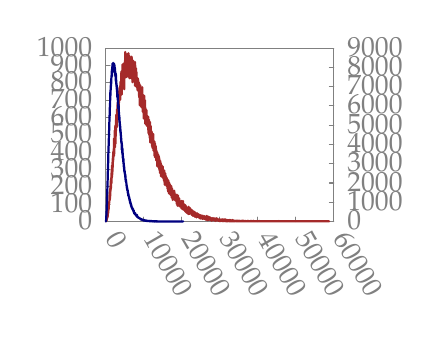
\begin{tikzpicture}[gnuplot, scale=0.3]
%% generated with GNUPLOT 5.2p2 (Lua 5.3; terminal rev. 99, script rev. 102)
%% wo 11 jul 2018 09:51:59 CEST
\path (0.000,0.000) rectangle (12.500,8.750);
\gpcolor{rgb color={0.502,0.502,0.502}}
\gpsetlinetype{gp lt border}
\gpsetdashtype{gp dt solid}
\gpsetlinewidth{1.00}
\draw[gp path] (1.196,1.104)--(1.376,1.104);
\node[gp node right] at (1.012,1.104) {$0$};
\draw[gp path] (1.196,1.838)--(1.376,1.838);
\node[gp node right] at (1.012,1.838) {$100$};
\draw[gp path] (1.196,2.571)--(1.376,2.571);
\node[gp node right] at (1.012,2.571) {$200$};
\draw[gp path] (1.196,3.305)--(1.376,3.305);
\node[gp node right] at (1.012,3.305) {$300$};
\draw[gp path] (1.196,4.039)--(1.376,4.039);
\node[gp node right] at (1.012,4.039) {$400$};
\draw[gp path] (1.196,4.773)--(1.376,4.773);
\node[gp node right] at (1.012,4.773) {$500$};
\draw[gp path] (1.196,5.506)--(1.376,5.506);
\node[gp node right] at (1.012,5.506) {$600$};
\draw[gp path] (1.196,6.240)--(1.376,6.240);
\node[gp node right] at (1.012,6.240) {$700$};
\draw[gp path] (1.196,6.974)--(1.376,6.974);
\node[gp node right] at (1.012,6.974) {$800$};
\draw[gp path] (1.196,7.707)--(1.376,7.707);
\node[gp node right] at (1.012,7.707) {$900$};
\draw[gp path] (1.196,8.441)--(1.376,8.441);
\node[gp node right] at (1.012,8.441) {$1000$};
\draw[gp path] (1.196,1.104)--(1.196,1.284);
\node[gp node left,rotate=-60] at (1.196,0.920) {$0$};
\draw[gp path] (2.804,1.104)--(2.804,1.284);
\node[gp node left,rotate=-60] at (2.804,0.920) {$10000$};
\draw[gp path] (4.412,1.104)--(4.412,1.284);
\node[gp node left,rotate=-60] at (4.412,0.920) {$20000$};
\draw[gp path] (6.020,1.104)--(6.020,1.284);
\node[gp node left,rotate=-60] at (6.020,0.920) {$30000$};
\draw[gp path] (7.627,1.104)--(7.627,1.284);
\node[gp node left,rotate=-60] at (7.627,0.920) {$40000$};
\draw[gp path] (9.235,1.104)--(9.235,1.284);
\node[gp node left,rotate=-60] at (9.235,0.920) {$50000$};
\draw[gp path] (10.843,1.104)--(10.843,1.284);
\node[gp node left,rotate=-60] at (10.843,0.920) {$60000$};
\draw[gp path] (10.843,1.104)--(10.663,1.104);
\node[gp node left] at (11.027,1.104) {$0$};
\draw[gp path] (10.843,1.919)--(10.663,1.919);
\node[gp node left] at (11.027,1.919) {$1000$};
\draw[gp path] (10.843,2.734)--(10.663,2.734);
\node[gp node left] at (11.027,2.734) {$2000$};
\draw[gp path] (10.843,3.550)--(10.663,3.550);
\node[gp node left] at (11.027,3.550) {$3000$};
\draw[gp path] (10.843,4.365)--(10.663,4.365);
\node[gp node left] at (11.027,4.365) {$4000$};
\draw[gp path] (10.843,5.180)--(10.663,5.180);
\node[gp node left] at (11.027,5.180) {$5000$};
\draw[gp path] (10.843,5.995)--(10.663,5.995);
\node[gp node left] at (11.027,5.995) {$6000$};
\draw[gp path] (10.843,6.811)--(10.663,6.811);
\node[gp node left] at (11.027,6.811) {$7000$};
\draw[gp path] (10.843,7.626)--(10.663,7.626);
\node[gp node left] at (11.027,7.626) {$8000$};
\draw[gp path] (10.843,8.441)--(10.663,8.441);
\node[gp node left] at (11.027,8.441) {$9000$};
\draw[gp path] (1.196,8.441)--(1.196,1.104)--(10.843,1.104)--(10.843,8.441)--cycle;
\gpcolor{rgb color={0.647,0.165,0.165}}
\gpsetlinewidth{2.00}
\draw[gp path] (1.207,1.119)--(1.209,1.111)--(1.210,1.126)--(1.212,1.126)--(1.214,1.126)%
  --(1.215,1.126)--(1.217,1.141)--(1.219,1.141)--(1.220,1.119)--(1.222,1.148)--(1.223,1.141)%
  --(1.225,1.163)--(1.227,1.163)--(1.228,1.126)--(1.230,1.155)--(1.231,1.148)--(1.233,1.192)%
  --(1.235,1.192)--(1.236,1.177)--(1.238,1.185)--(1.239,1.199)--(1.241,1.214)--(1.243,1.287)%
  --(1.244,1.214)--(1.246,1.273)--(1.247,1.207)--(1.249,1.236)--(1.251,1.236)--(1.252,1.265)%
  --(1.254,1.287)--(1.255,1.273)--(1.257,1.295)--(1.259,1.251)--(1.260,1.287)--(1.262,1.287)%
  --(1.264,1.317)--(1.265,1.361)--(1.267,1.273)--(1.268,1.346)--(1.270,1.295)--(1.272,1.302)%
  --(1.273,1.478)--(1.275,1.434)--(1.276,1.309)--(1.278,1.434)--(1.280,1.346)--(1.281,1.390)%
  --(1.283,1.442)--(1.284,1.500)--(1.286,1.449)--(1.288,1.449)--(1.289,1.500)--(1.291,1.434)%
  --(1.292,1.581)--(1.294,1.493)--(1.296,1.486)--(1.297,1.559)--(1.299,1.559)--(1.301,1.478)%
  --(1.302,1.640)--(1.304,1.530)--(1.305,1.574)--(1.307,1.618)--(1.309,1.764)--(1.310,1.596)%
  --(1.312,1.764)--(1.313,1.618)--(1.315,1.676)--(1.317,1.698)--(1.318,1.654)--(1.320,1.779)%
  --(1.321,1.786)--(1.323,1.684)--(1.325,1.640)--(1.326,1.801)--(1.328,1.896)--(1.329,1.860)%
  --(1.331,1.830)--(1.333,1.852)--(1.334,1.889)--(1.336,1.918)--(1.337,1.926)--(1.339,1.933)%
  --(1.341,1.933)--(1.342,1.948)--(1.344,1.896)--(1.346,1.918)--(1.347,2.050)--(1.349,2.219)%
  --(1.350,2.124)--(1.352,2.168)--(1.354,2.102)--(1.355,2.168)--(1.357,2.058)--(1.358,2.117)%
  --(1.360,2.293)--(1.362,2.285)--(1.363,2.036)--(1.365,2.006)--(1.366,2.344)--(1.368,2.175)%
  --(1.370,2.241)--(1.371,2.072)--(1.373,2.395)--(1.374,2.263)--(1.376,2.219)--(1.378,2.080)%
  --(1.379,2.263)--(1.381,2.175)--(1.383,2.381)--(1.384,2.329)--(1.386,2.417)--(1.387,2.505)%
  --(1.389,2.381)--(1.391,2.381)--(1.392,2.432)--(1.394,2.593)--(1.395,2.417)--(1.397,2.557)%
  --(1.399,2.630)--(1.400,2.461)--(1.402,2.608)--(1.403,2.527)--(1.405,2.821)--(1.407,2.681)%
  --(1.408,2.601)--(1.410,2.469)--(1.411,2.542)--(1.413,2.520)--(1.415,2.858)--(1.416,2.725)%
  --(1.418,2.674)--(1.419,2.902)--(1.421,2.733)--(1.423,2.718)--(1.424,2.843)--(1.426,2.946)%
  --(1.428,2.777)--(1.429,2.850)--(1.431,2.997)--(1.432,3.041)--(1.434,2.725)--(1.436,2.806)%
  --(1.437,2.718)--(1.439,3.070)--(1.440,2.982)--(1.442,3.298)--(1.444,3.136)--(1.445,2.946)%
  --(1.447,3.232)--(1.448,3.114)--(1.450,3.246)--(1.452,3.063)--(1.453,2.975)--(1.455,3.107)%
  --(1.456,3.048)--(1.458,3.048)--(1.460,3.474)--(1.461,3.393)--(1.463,3.254)--(1.465,3.254)%
  --(1.466,3.232)--(1.468,3.268)--(1.469,3.327)--(1.471,3.202)--(1.473,3.092)--(1.474,3.246)%
  --(1.476,3.415)--(1.477,3.606)--(1.479,3.290)--(1.481,3.217)--(1.482,3.312)--(1.484,3.591)%
  --(1.485,3.569)--(1.487,3.650)--(1.489,3.621)--(1.490,3.437)--(1.492,3.775)--(1.493,3.400)%
  --(1.495,3.577)--(1.497,3.701)--(1.498,3.885)--(1.500,3.650)--(1.501,3.745)--(1.503,3.701)%
  --(1.505,3.797)--(1.506,4.046)--(1.508,3.789)--(1.510,3.738)--(1.511,3.892)--(1.513,3.782)%
  --(1.514,3.709)--(1.516,3.877)--(1.518,4.068)--(1.519,3.833)--(1.521,4.017)--(1.522,3.958)%
  --(1.524,3.914)--(1.526,4.112)--(1.527,4.002)--(1.529,3.907)--(1.530,4.105)--(1.532,4.097)%
  --(1.534,4.112)--(1.535,3.958)--(1.537,4.288)--(1.538,3.958)--(1.540,3.987)--(1.542,4.090)%
  --(1.543,4.618)--(1.545,4.031)--(1.547,4.075)--(1.548,3.892)--(1.550,4.186)--(1.551,4.523)%
  --(1.553,4.523)--(1.555,4.149)--(1.556,4.186)--(1.558,4.611)--(1.559,4.222)--(1.561,4.369)%
  --(1.563,4.310)--(1.564,4.486)--(1.566,4.516)--(1.567,4.420)--(1.569,4.508)--(1.571,4.611)%
  --(1.572,4.384)--(1.574,4.956)--(1.575,4.567)--(1.577,4.582)--(1.579,4.369)--(1.580,4.589)%
  --(1.582,4.244)--(1.583,4.479)--(1.585,4.883)--(1.587,4.523)--(1.588,4.677)--(1.590,4.787)%
  --(1.592,4.552)--(1.593,4.648)--(1.595,4.949)--(1.596,4.963)--(1.598,4.545)--(1.600,5.176)%
  --(1.601,4.596)--(1.603,4.391)--(1.604,4.963)--(1.606,4.846)--(1.608,4.824)--(1.609,4.706)%
  --(1.611,4.802)--(1.612,4.706)--(1.614,5.169)--(1.616,5.073)--(1.617,5.081)--(1.619,4.897)%
  --(1.620,5.000)--(1.622,4.905)--(1.624,5.000)--(1.625,5.411)--(1.627,5.000)--(1.629,5.132)%
  --(1.630,5.176)--(1.632,5.286)--(1.633,5.323)--(1.635,5.616)--(1.637,5.345)--(1.638,5.154)%
  --(1.640,5.433)--(1.641,5.433)--(1.643,5.125)--(1.645,5.337)--(1.646,5.191)--(1.648,5.088)%
  --(1.649,5.169)--(1.651,5.514)--(1.653,5.345)--(1.654,5.308)--(1.656,5.095)--(1.657,5.117)%
  --(1.659,5.536)--(1.661,5.543)--(1.662,5.433)--(1.664,5.161)--(1.665,5.668)--(1.667,5.719)%
  --(1.669,5.807)--(1.670,5.851)--(1.672,5.367)--(1.674,5.668)--(1.675,5.448)--(1.677,5.293)%
  --(1.678,5.756)--(1.680,5.367)--(1.682,5.506)--(1.683,5.609)--(1.685,5.631)--(1.686,5.565)%
  --(1.688,5.558)--(1.690,5.506)--(1.691,5.932)--(1.693,5.565)--(1.694,6.049)--(1.696,5.748)%
  --(1.698,5.851)--(1.699,5.697)--(1.701,5.631)--(1.702,5.653)--(1.704,6.145)--(1.706,5.800)%
  --(1.707,5.800)--(1.709,5.844)--(1.711,5.558)--(1.712,5.572)--(1.714,5.910)--(1.715,5.895)%
  --(1.717,6.262)--(1.719,5.814)--(1.720,6.056)--(1.722,5.954)--(1.723,5.910)--(1.725,5.924)%
  --(1.727,6.225)--(1.728,6.049)--(1.730,6.482)--(1.731,6.387)--(1.733,6.306)--(1.735,6.291)%
  --(1.736,6.086)--(1.738,5.880)--(1.739,5.836)--(1.741,6.306)--(1.743,6.189)--(1.744,6.519)%
  --(1.746,6.189)--(1.747,6.042)--(1.749,6.145)--(1.751,6.130)--(1.752,6.365)--(1.754,6.291)%
  --(1.756,6.233)--(1.757,6.269)--(1.759,6.203)--(1.760,6.621)--(1.762,6.255)--(1.764,6.225)%
  --(1.765,6.504)--(1.767,6.599)--(1.768,6.423)--(1.770,6.761)--(1.772,6.321)--(1.773,6.306)%
  --(1.775,6.328)--(1.776,6.306)--(1.778,6.482)--(1.780,6.357)--(1.781,6.343)--(1.783,6.438)%
  --(1.784,6.328)--(1.786,6.489)--(1.788,6.702)--(1.789,6.255)--(1.791,6.812)--(1.793,6.665)%
  --(1.794,6.423)--(1.796,6.467)--(1.797,6.577)--(1.799,6.563)--(1.801,6.247)--(1.802,6.504)%
  --(1.804,6.269)--(1.805,6.614)--(1.807,6.849)--(1.809,6.731)--(1.810,6.702)--(1.812,6.570)%
  --(1.813,7.010)--(1.815,6.871)--(1.817,6.555)--(1.818,6.739)--(1.820,6.739)--(1.821,6.680)%
  --(1.823,6.563)--(1.825,6.966)--(1.826,6.900)--(1.828,6.739)--(1.829,6.636)--(1.831,6.805)%
  --(1.833,6.680)--(1.834,6.746)--(1.836,6.636)--(1.838,6.511)--(1.839,7.054)--(1.841,6.636)%
  --(1.842,6.937)--(1.844,7.003)--(1.846,7.098)--(1.847,7.194)--(1.849,6.768)--(1.850,6.893)%
  --(1.852,6.680)--(1.854,7.458)--(1.855,6.864)--(1.857,7.032)--(1.858,6.849)--(1.860,6.981)%
  --(1.862,7.098)--(1.863,6.820)--(1.865,7.062)--(1.866,6.621)--(1.868,6.724)--(1.870,7.106)%
  --(1.871,6.475)--(1.873,7.025)--(1.875,6.695)--(1.876,6.922)--(1.878,7.047)--(1.879,7.179)%
  --(1.881,7.172)--(1.883,7.194)--(1.884,7.443)--(1.886,7.076)--(1.887,7.238)--(1.889,6.915)%
  --(1.891,6.996)--(1.892,7.230)--(1.894,7.172)--(1.895,6.988)--(1.897,7.311)--(1.899,7.575)%
  --(1.900,7.751)--(1.902,7.230)--(1.903,7.230)--(1.905,6.878)--(1.907,7.032)--(1.908,7.414)%
  --(1.910,6.908)--(1.911,7.098)--(1.913,7.194)--(1.915,7.267)--(1.916,7.164)--(1.918,7.120)%
  --(1.920,7.098)--(1.921,7.047)--(1.923,7.590)--(1.924,6.783)--(1.926,7.495)--(1.928,7.274)%
  --(1.929,7.495)--(1.931,7.414)--(1.932,7.091)--(1.934,7.010)--(1.936,7.069)--(1.937,7.326)%
  --(1.939,7.495)--(1.940,7.436)--(1.942,7.326)--(1.944,7.612)--(1.945,7.524)--(1.947,7.436)%
  --(1.948,7.311)--(1.950,7.443)--(1.952,7.465)--(1.953,7.384)--(1.955,7.340)--(1.957,7.223)%
  --(1.958,7.619)--(1.960,7.326)--(1.961,7.597)--(1.963,7.318)--(1.965,7.803)--(1.966,7.318)%
  --(1.968,7.362)--(1.969,7.649)--(1.971,7.553)--(1.973,7.502)--(1.974,7.693)--(1.976,6.702)%
  --(1.977,7.421)--(1.979,7.663)--(1.981,7.781)--(1.982,7.649)--(1.984,7.487)--(1.985,7.583)%
  --(1.987,7.715)--(1.989,7.399)--(1.990,7.517)--(1.992,7.487)--(1.993,7.693)--(1.995,7.619)%
  --(1.997,7.509)--(1.998,7.788)--(2.000,7.428)--(2.002,7.612)--(2.003,7.913)--(2.005,7.340)%
  --(2.006,7.355)--(2.008,7.509)--(2.010,7.340)--(2.011,7.436)--(2.013,7.311)--(2.014,7.414)%
  --(2.016,7.971)--(2.018,7.428)--(2.019,7.480)--(2.021,7.377)--(2.022,8.280)--(2.024,7.289)%
  --(2.026,7.641)--(2.027,7.649)--(2.029,7.451)--(2.030,7.663)--(2.032,7.597)--(2.034,7.634)%
  --(2.035,7.700)--(2.037,7.619)--(2.039,7.817)--(2.040,7.414)--(2.042,7.208)--(2.043,7.715)%
  --(2.045,7.230)--(2.047,7.465)--(2.048,7.517)--(2.050,7.487)--(2.051,7.458)--(2.053,7.465)%
  --(2.055,7.810)--(2.056,7.465)--(2.058,7.700)--(2.059,7.583)--(2.061,7.751)--(2.063,7.443)%
  --(2.064,7.715)--(2.066,7.707)--(2.067,7.399)--(2.069,7.304)--(2.071,7.597)--(2.072,7.223)%
  --(2.074,7.612)--(2.075,7.619)--(2.077,7.766)--(2.079,7.671)--(2.080,7.744)--(2.082,7.663)%
  --(2.084,7.649)--(2.085,7.590)--(2.087,7.766)--(2.088,8.074)--(2.090,8.023)--(2.092,7.839)%
  --(2.093,7.304)--(2.095,7.949)--(2.096,7.619)--(2.098,7.428)--(2.100,7.913)--(2.101,7.898)%
  --(2.103,7.495)--(2.104,7.392)--(2.106,8.052)--(2.108,7.964)--(2.109,7.392)--(2.111,7.788)%
  --(2.112,8.081)--(2.114,7.920)--(2.116,7.891)--(2.117,7.473)--(2.119,8.170)--(2.121,8.206)%
  --(2.122,7.795)--(2.124,7.913)--(2.125,7.722)--(2.127,7.627)--(2.129,7.803)--(2.130,7.781)%
  --(2.132,8.037)--(2.133,7.605)--(2.135,7.421)--(2.137,7.238)--(2.138,7.876)--(2.140,7.722)%
  --(2.141,7.737)--(2.143,7.847)--(2.145,7.993)--(2.146,7.502)--(2.148,7.707)--(2.149,8.133)%
  --(2.151,7.832)--(2.153,7.649)--(2.154,7.715)--(2.156,7.685)--(2.157,8.228)--(2.159,7.788)%
  --(2.161,7.927)--(2.162,7.583)--(2.164,7.524)--(2.166,7.722)--(2.167,7.605)--(2.169,7.641)%
  --(2.170,8.008)--(2.172,7.971)--(2.174,7.612)--(2.175,7.451)--(2.177,7.428)--(2.178,7.634)%
  --(2.180,7.597)--(2.182,8.008)--(2.183,7.707)--(2.185,7.539)--(2.186,7.832)--(2.188,7.964)%
  --(2.190,7.729)--(2.191,7.751)--(2.193,8.111)--(2.194,7.773)--(2.196,7.942)--(2.198,7.575)%
  --(2.199,7.164)--(2.201,7.685)--(2.203,7.759)--(2.204,7.473)--(2.206,7.832)--(2.207,7.773)%
  --(2.209,7.935)--(2.211,7.722)--(2.212,8.001)--(2.214,7.685)--(2.215,7.619)--(2.217,7.795)%
  --(2.219,7.561)--(2.220,7.216)--(2.222,7.179)--(2.223,7.729)--(2.225,7.304)--(2.227,7.693)%
  --(2.228,7.495)--(2.230,7.590)--(2.231,7.737)--(2.233,7.781)--(2.235,7.649)--(2.236,7.759)%
  --(2.238,7.949)--(2.239,7.913)--(2.241,7.671)--(2.243,7.414)--(2.244,7.971)--(2.246,7.539)%
  --(2.248,7.480)--(2.249,7.788)--(2.251,7.605)--(2.252,7.605)--(2.254,7.854)--(2.256,7.605)%
  --(2.257,7.406)--(2.259,7.304)--(2.260,7.788)--(2.262,7.663)--(2.264,7.340)--(2.265,7.531)%
  --(2.267,7.773)--(2.268,7.539)--(2.270,7.531)--(2.272,7.487)--(2.273,7.473)--(2.275,7.751)%
  --(2.276,7.766)--(2.278,7.583)--(2.280,7.700)--(2.281,7.847)--(2.283,7.619)--(2.285,7.920)%
  --(2.286,7.971)--(2.288,8.081)--(2.289,7.649)--(2.291,7.384)--(2.293,7.465)--(2.294,7.590)%
  --(2.296,8.045)--(2.297,7.142)--(2.299,7.451)--(2.301,7.759)--(2.302,7.649)--(2.304,7.487)%
  --(2.305,7.524)--(2.307,7.495)--(2.309,7.480)--(2.310,7.751)--(2.312,7.722)--(2.313,7.274)%
  --(2.315,7.333)--(2.317,7.399)--(2.318,7.355)--(2.320,7.766)--(2.321,7.370)--(2.323,7.436)%
  --(2.325,7.480)--(2.326,6.996)--(2.328,7.355)--(2.330,7.539)--(2.331,7.362)--(2.333,7.157)%
  --(2.334,7.399)--(2.336,7.766)--(2.338,7.641)--(2.339,7.575)--(2.341,7.656)--(2.342,7.340)%
  --(2.344,7.766)--(2.346,7.502)--(2.347,7.517)--(2.349,7.311)--(2.350,7.370)--(2.352,7.693)%
  --(2.354,7.509)--(2.355,7.451)--(2.357,7.905)--(2.358,7.803)--(2.360,7.414)--(2.362,7.546)%
  --(2.363,7.612)--(2.365,7.370)--(2.367,7.854)--(2.368,7.495)--(2.370,7.355)--(2.371,7.524)%
  --(2.373,7.150)--(2.375,7.671)--(2.376,7.465)--(2.378,7.245)--(2.379,7.392)--(2.381,7.678)%
  --(2.383,7.054)--(2.384,7.370)--(2.386,7.737)--(2.387,7.531)--(2.389,7.296)--(2.391,7.458)%
  --(2.392,7.458)--(2.394,7.436)--(2.395,7.150)--(2.397,7.627)--(2.399,7.421)--(2.400,7.825)%
  --(2.402,7.223)--(2.403,7.377)--(2.405,7.473)--(2.407,7.260)--(2.408,7.539)--(2.410,7.428)%
  --(2.412,7.267)--(2.413,7.296)--(2.415,7.216)--(2.416,7.289)--(2.418,7.546)--(2.420,7.047)%
  --(2.421,7.311)--(2.423,7.040)--(2.424,7.399)--(2.426,7.274)--(2.428,7.282)--(2.429,6.849)%
  --(2.431,7.370)--(2.432,7.333)--(2.434,7.157)--(2.436,7.854)--(2.437,7.399)--(2.439,7.348)%
  --(2.440,7.091)--(2.442,7.348)--(2.444,7.223)--(2.445,7.296)--(2.447,7.707)--(2.449,7.040)%
  --(2.450,7.568)--(2.452,7.040)--(2.453,7.384)--(2.455,7.223)--(2.457,6.959)--(2.458,7.362)%
  --(2.460,7.428)--(2.461,7.194)--(2.463,7.289)--(2.465,6.915)--(2.466,7.252)--(2.468,7.084)%
  --(2.469,7.216)--(2.471,7.260)--(2.473,7.179)--(2.474,7.238)--(2.476,7.590)--(2.477,6.988)%
  --(2.479,7.113)--(2.481,6.974)--(2.482,6.981)--(2.484,6.893)--(2.485,7.252)--(2.487,7.451)%
  --(2.489,6.981)--(2.490,6.952)--(2.492,7.421)--(2.494,7.157)--(2.495,6.798)--(2.497,7.201)%
  --(2.498,7.362)--(2.500,6.981)--(2.502,7.091)--(2.503,7.157)--(2.505,7.047)--(2.506,7.003)%
  --(2.508,7.032)--(2.510,7.135)--(2.511,6.996)--(2.513,7.091)--(2.514,7.018)--(2.516,7.018)%
  --(2.518,7.186)--(2.519,7.003)--(2.521,6.798)--(2.522,7.025)--(2.524,7.010)--(2.526,6.753)%
  --(2.527,6.753)--(2.529,7.106)--(2.531,6.886)--(2.532,6.842)--(2.534,6.673)--(2.535,6.974)%
  --(2.537,6.776)--(2.539,6.827)--(2.540,7.084)--(2.542,6.651)--(2.543,6.922)--(2.545,6.908)%
  --(2.547,6.959)--(2.548,6.871)--(2.550,7.047)--(2.551,6.952)--(2.553,7.164)--(2.555,6.966)%
  --(2.556,6.812)--(2.558,7.025)--(2.559,6.886)--(2.561,7.003)--(2.563,6.753)--(2.564,7.135)%
  --(2.566,6.856)--(2.567,7.018)--(2.569,6.849)--(2.571,6.665)--(2.572,6.849)--(2.574,6.878)%
  --(2.576,6.966)--(2.577,6.665)--(2.579,6.820)--(2.580,6.665)--(2.582,6.798)--(2.584,6.702)%
  --(2.585,6.695)--(2.587,6.658)--(2.588,6.834)--(2.590,6.996)--(2.592,6.739)--(2.593,6.739)%
  --(2.595,6.849)--(2.596,6.629)--(2.598,6.959)--(2.600,6.702)--(2.601,6.629)--(2.603,6.687)%
  --(2.604,6.431)--(2.606,6.497)--(2.608,6.467)--(2.609,6.937)--(2.611,6.599)--(2.613,6.607)%
  --(2.614,6.365)--(2.616,6.585)--(2.617,6.768)--(2.619,6.900)--(2.621,6.526)--(2.622,6.343)%
  --(2.624,6.878)--(2.625,6.607)--(2.627,6.475)--(2.629,6.687)--(2.630,6.027)--(2.632,6.790)%
  --(2.633,6.585)--(2.635,6.262)--(2.637,6.555)--(2.638,6.599)--(2.640,6.739)--(2.641,6.372)%
  --(2.643,6.731)--(2.645,6.665)--(2.646,6.695)--(2.648,6.651)--(2.649,6.159)--(2.651,6.482)%
  --(2.653,6.871)--(2.654,6.651)--(2.656,6.445)--(2.658,6.357)--(2.659,6.467)--(2.661,6.145)%
  --(2.662,6.489)--(2.664,5.990)--(2.666,6.431)--(2.667,6.746)--(2.669,6.709)--(2.670,6.255)%
  --(2.672,6.277)--(2.674,6.365)--(2.675,6.790)--(2.677,6.614)--(2.678,6.658)--(2.680,6.372)%
  --(2.682,6.636)--(2.683,6.262)--(2.685,6.189)--(2.686,6.269)--(2.688,6.533)--(2.690,6.328)%
  --(2.691,6.467)--(2.693,6.533)--(2.695,6.328)--(2.696,6.453)--(2.698,6.460)--(2.699,6.423)%
  --(2.701,6.328)--(2.703,6.401)--(2.704,6.379)--(2.706,5.939)--(2.707,6.123)--(2.709,6.592)%
  --(2.711,6.753)--(2.712,6.108)--(2.714,6.636)--(2.715,6.240)--(2.717,6.233)--(2.719,6.519)%
  --(2.720,6.335)--(2.722,6.159)--(2.723,6.379)--(2.725,6.497)--(2.727,6.203)--(2.728,6.321)%
  --(2.730,6.577)--(2.731,6.167)--(2.733,6.123)--(2.735,6.064)--(2.736,6.790)--(2.738,6.027)%
  --(2.740,6.086)--(2.741,6.423)--(2.743,6.108)--(2.744,6.020)--(2.746,6.350)--(2.748,6.277)%
  --(2.749,6.100)--(2.751,6.262)--(2.752,5.946)--(2.754,6.255)--(2.756,6.467)--(2.757,6.100)%
  --(2.759,5.836)--(2.760,5.748)--(2.762,6.475)--(2.764,6.078)--(2.765,6.181)--(2.767,6.416)%
  --(2.768,6.020)--(2.770,6.064)--(2.772,6.005)--(2.773,5.792)--(2.775,6.328)--(2.777,6.086)%
  --(2.778,5.939)--(2.780,6.049)--(2.781,6.078)--(2.783,6.152)--(2.785,6.071)--(2.786,6.247)%
  --(2.788,6.159)--(2.789,5.697)--(2.791,6.100)--(2.793,5.822)--(2.794,6.225)--(2.796,5.976)%
  --(2.797,5.682)--(2.799,5.785)--(2.801,5.873)--(2.802,5.462)--(2.804,5.785)--(2.805,5.609)%
  --(2.807,6.086)--(2.809,5.682)--(2.810,5.968)--(2.812,6.071)--(2.813,5.778)--(2.815,5.770)%
  --(2.817,5.998)--(2.818,5.866)--(2.820,6.071)--(2.822,6.152)--(2.823,6.423)--(2.825,5.990)%
  --(2.826,5.954)--(2.828,6.321)--(2.830,5.946)--(2.831,5.448)--(2.833,5.697)--(2.834,5.778)%
  --(2.836,5.704)--(2.838,5.646)--(2.839,6.020)--(2.841,5.910)--(2.842,5.778)--(2.844,5.873)%
  --(2.846,6.078)--(2.847,5.528)--(2.849,5.800)--(2.850,5.763)--(2.852,5.822)--(2.854,5.712)%
  --(2.855,5.939)--(2.857,6.233)--(2.858,5.829)--(2.860,5.741)--(2.862,5.484)--(2.863,5.660)%
  --(2.865,5.624)--(2.867,5.924)--(2.868,5.235)--(2.870,5.668)--(2.871,5.425)--(2.873,5.403)%
  --(2.875,5.528)--(2.876,5.822)--(2.878,5.550)--(2.879,5.572)--(2.881,5.609)--(2.883,5.499)%
  --(2.884,5.425)--(2.886,5.499)--(2.887,5.726)--(2.889,5.536)--(2.891,5.770)--(2.892,5.506)%
  --(2.894,5.858)--(2.895,5.271)--(2.897,5.565)--(2.899,5.264)--(2.900,5.381)--(2.902,5.440)%
  --(2.904,5.440)--(2.905,5.492)--(2.907,5.514)--(2.908,5.396)--(2.910,5.455)--(2.912,5.418)%
  --(2.913,5.359)--(2.915,5.646)--(2.916,5.712)--(2.918,5.271)--(2.920,5.807)--(2.921,5.778)%
  --(2.923,5.345)--(2.924,5.565)--(2.926,5.359)--(2.928,5.154)--(2.929,5.528)--(2.931,5.536)%
  --(2.932,5.492)--(2.934,5.506)--(2.936,5.587)--(2.937,5.227)--(2.939,5.227)--(2.940,5.301)%
  --(2.942,5.308)--(2.944,5.323)--(2.945,5.286)--(2.947,5.396)--(2.949,5.352)--(2.950,5.455)%
  --(2.952,5.308)--(2.953,5.359)--(2.955,5.528)--(2.957,5.572)--(2.958,5.352)--(2.960,5.411)%
  --(2.961,5.191)--(2.963,5.425)--(2.965,5.337)--(2.966,5.227)--(2.968,5.492)--(2.969,5.330)%
  --(2.971,5.345)--(2.973,5.425)--(2.974,5.132)--(2.976,5.139)--(2.977,5.396)--(2.979,5.264)%
  --(2.981,5.103)--(2.982,5.132)--(2.984,5.337)--(2.986,5.235)--(2.987,5.521)--(2.989,5.323)%
  --(2.990,5.125)--(2.992,5.425)--(2.994,5.088)--(2.995,4.971)--(2.997,5.323)--(2.998,5.536)%
  --(3.000,4.846)--(3.002,5.286)--(3.003,5.315)--(3.005,5.227)--(3.006,5.330)--(3.008,5.183)%
  --(3.010,5.220)--(3.011,5.337)--(3.013,5.213)--(3.014,5.183)--(3.016,5.044)--(3.018,4.941)%
  --(3.019,5.308)--(3.021,4.978)--(3.022,5.418)--(3.024,5.044)--(3.026,4.817)--(3.027,5.198)%
  --(3.029,5.220)--(3.031,5.147)--(3.032,5.249)--(3.034,5.198)--(3.035,5.022)--(3.037,4.765)%
  --(3.039,5.000)--(3.040,4.802)--(3.042,4.993)--(3.043,5.015)--(3.045,4.861)--(3.047,4.824)%
  --(3.048,4.831)--(3.050,5.213)--(3.051,5.139)--(3.053,5.249)--(3.055,4.633)--(3.056,5.169)%
  --(3.058,4.787)--(3.059,4.949)--(3.061,5.051)--(3.063,4.809)--(3.064,5.315)--(3.066,5.044)%
  --(3.068,4.971)--(3.069,4.795)--(3.071,4.831)--(3.072,5.007)--(3.074,4.985)--(3.076,4.758)%
  --(3.077,4.971)--(3.079,4.450)--(3.080,4.839)--(3.082,5.000)--(3.084,5.125)--(3.085,5.051)%
  --(3.087,4.905)--(3.088,4.765)--(3.090,4.897)--(3.092,4.714)--(3.093,4.971)--(3.095,4.714)%
  --(3.096,4.765)--(3.098,4.538)--(3.100,4.846)--(3.101,4.773)--(3.103,5.139)--(3.104,4.934)%
  --(3.106,4.765)--(3.108,4.978)--(3.109,4.795)--(3.111,4.758)--(3.113,4.670)--(3.114,4.692)%
  --(3.116,4.750)--(3.117,4.662)--(3.119,4.655)--(3.121,4.640)--(3.122,4.567)--(3.124,4.567)%
  --(3.125,4.773)--(3.127,4.662)--(3.129,4.560)--(3.130,4.662)--(3.132,4.538)--(3.133,4.538)%
  --(3.135,4.670)--(3.137,4.472)--(3.138,4.699)--(3.140,4.530)--(3.141,4.905)--(3.143,4.662)%
  --(3.145,4.516)--(3.146,4.530)--(3.148,4.288)--(3.150,4.626)--(3.151,4.677)--(3.153,4.640)%
  --(3.154,4.824)--(3.156,4.743)--(3.158,4.750)--(3.159,4.545)--(3.161,4.486)--(3.162,4.486)%
  --(3.164,4.523)--(3.166,4.464)--(3.167,4.428)--(3.169,4.670)--(3.170,4.736)--(3.172,4.406)%
  --(3.174,4.523)--(3.175,4.215)--(3.177,4.391)--(3.178,4.435)--(3.180,4.369)--(3.182,4.494)%
  --(3.183,4.626)--(3.185,4.545)--(3.186,4.376)--(3.188,4.486)--(3.190,4.662)--(3.191,4.325)%
  --(3.193,4.589)--(3.195,4.450)--(3.196,4.552)--(3.198,4.420)--(3.199,4.398)--(3.201,4.765)%
  --(3.203,4.369)--(3.204,4.611)--(3.206,4.809)--(3.207,4.362)--(3.209,4.479)--(3.211,4.097)%
  --(3.212,4.266)--(3.214,4.384)--(3.215,4.398)--(3.217,4.472)--(3.219,4.149)--(3.220,4.369)%
  --(3.222,4.288)--(3.223,4.200)--(3.225,4.486)--(3.227,4.208)--(3.228,4.266)--(3.230,4.428)%
  --(3.232,4.310)--(3.233,4.376)--(3.235,4.310)--(3.236,4.244)--(3.238,4.332)--(3.240,4.406)%
  --(3.241,4.252)--(3.243,4.296)--(3.244,4.486)--(3.246,4.288)--(3.248,4.222)--(3.249,4.494)%
  --(3.251,4.237)--(3.252,4.222)--(3.254,4.244)--(3.256,4.303)--(3.257,4.479)--(3.259,3.885)%
  --(3.260,4.296)--(3.262,4.354)--(3.264,4.105)--(3.265,4.340)--(3.267,4.406)--(3.268,4.002)%
  --(3.270,4.164)--(3.272,4.281)--(3.273,4.318)--(3.275,4.222)--(3.277,3.826)--(3.278,4.017)%
  --(3.280,4.406)--(3.281,4.149)--(3.283,4.230)--(3.285,4.288)--(3.286,4.186)--(3.288,4.061)%
  --(3.289,4.164)--(3.291,4.127)--(3.293,4.332)--(3.294,4.061)--(3.296,3.987)--(3.297,3.899)%
  --(3.299,3.980)--(3.301,4.259)--(3.302,4.193)--(3.304,4.310)--(3.305,4.017)--(3.307,4.120)%
  --(3.309,4.046)--(3.310,4.178)--(3.312,3.958)--(3.314,4.281)--(3.315,3.885)--(3.317,4.193)%
  --(3.318,4.068)--(3.320,3.855)--(3.322,4.142)--(3.323,3.892)--(3.325,3.951)--(3.326,3.877)%
  --(3.328,3.958)--(3.330,4.090)--(3.331,3.943)--(3.333,3.687)--(3.334,4.097)--(3.336,3.745)%
  --(3.338,3.811)--(3.339,3.701)--(3.341,3.760)--(3.342,3.936)--(3.344,3.914)--(3.346,4.024)%
  --(3.347,4.090)--(3.349,3.907)--(3.350,3.848)--(3.352,4.053)--(3.354,3.848)--(3.355,3.958)%
  --(3.357,3.936)--(3.359,3.914)--(3.360,3.921)--(3.362,3.841)--(3.363,3.943)--(3.365,3.936)%
  --(3.367,4.031)--(3.368,4.009)--(3.370,4.031)--(3.371,3.951)--(3.373,3.635)--(3.375,3.437)%
  --(3.376,3.540)--(3.378,3.907)--(3.379,3.599)--(3.381,3.709)--(3.383,3.540)--(3.384,3.987)%
  --(3.386,3.826)--(3.387,3.885)--(3.389,3.547)--(3.391,3.921)--(3.392,3.870)--(3.394,3.811)%
  --(3.396,3.841)--(3.397,3.709)--(3.399,3.687)--(3.400,3.877)--(3.402,3.833)--(3.404,3.782)%
  --(3.405,3.745)--(3.407,3.789)--(3.408,3.422)--(3.410,3.672)--(3.412,3.650)--(3.413,3.782)%
  --(3.415,3.701)--(3.416,3.914)--(3.418,3.650)--(3.420,3.489)--(3.421,3.921)--(3.423,3.811)%
  --(3.424,3.841)--(3.426,3.628)--(3.428,3.665)--(3.429,3.665)--(3.431,3.885)--(3.432,3.665)%
  --(3.434,3.804)--(3.436,3.804)--(3.437,3.694)--(3.439,3.870)--(3.441,3.841)--(3.442,3.613)%
  --(3.444,3.841)--(3.445,3.679)--(3.447,3.452)--(3.449,3.555)--(3.450,3.731)--(3.452,3.459)%
  --(3.453,3.386)--(3.455,3.525)--(3.457,3.415)--(3.458,3.569)--(3.460,3.643)--(3.461,3.327)%
  --(3.463,3.767)--(3.465,3.276)--(3.466,3.716)--(3.468,3.591)--(3.469,3.687)--(3.471,3.474)%
  --(3.473,3.613)--(3.474,3.650)--(3.476,3.445)--(3.478,3.613)--(3.479,3.650)--(3.481,3.503)%
  --(3.482,3.489)--(3.484,3.489)--(3.486,3.628)--(3.487,3.158)--(3.489,3.459)--(3.490,3.371)%
  --(3.492,3.334)--(3.494,3.562)--(3.495,3.320)--(3.497,3.400)--(3.498,3.672)--(3.500,3.562)%
  --(3.502,3.496)--(3.503,3.511)--(3.505,3.503)--(3.506,3.459)--(3.508,3.547)--(3.510,3.437)%
  --(3.511,3.415)--(3.513,3.320)--(3.514,3.180)--(3.516,3.525)--(3.518,3.400)--(3.519,3.422)%
  --(3.521,3.422)--(3.523,3.577)--(3.524,3.334)--(3.526,3.320)--(3.527,3.415)--(3.529,3.261)%
  --(3.531,3.232)--(3.532,3.371)--(3.534,3.349)--(3.535,3.012)--(3.537,3.378)--(3.539,3.386)%
  --(3.540,3.122)--(3.542,3.467)--(3.543,3.320)--(3.545,3.268)--(3.547,3.503)--(3.548,3.144)%
  --(3.550,3.158)--(3.551,3.180)--(3.553,3.283)--(3.555,3.489)--(3.556,3.327)--(3.558,3.122)%
  --(3.560,3.210)--(3.561,3.056)--(3.563,3.364)--(3.564,3.151)--(3.566,3.349)--(3.568,3.048)%
  --(3.569,3.070)--(3.571,3.070)--(3.572,3.312)--(3.574,3.202)--(3.576,3.232)--(3.577,3.019)%
  --(3.579,3.180)--(3.580,3.078)--(3.582,3.371)--(3.584,3.312)--(3.585,3.268)--(3.587,3.085)%
  --(3.588,3.349)--(3.590,3.085)--(3.592,3.393)--(3.593,2.975)--(3.595,3.048)--(3.596,3.210)%
  --(3.598,3.092)--(3.600,3.408)--(3.601,3.180)--(3.603,3.158)--(3.605,3.092)--(3.606,3.019)%
  --(3.608,3.107)--(3.609,3.129)--(3.611,3.430)--(3.613,3.034)--(3.614,3.092)--(3.616,3.158)%
  --(3.617,3.224)--(3.619,2.990)--(3.621,3.012)--(3.622,3.019)--(3.624,3.122)--(3.625,3.202)%
  --(3.627,3.078)--(3.629,3.092)--(3.630,3.217)--(3.632,3.151)--(3.633,2.968)--(3.635,3.210)%
  --(3.637,3.100)--(3.638,3.034)--(3.640,2.909)--(3.642,3.166)--(3.643,3.085)--(3.645,3.063)%
  --(3.646,2.997)--(3.648,2.894)--(3.650,2.931)--(3.651,3.092)--(3.653,3.026)--(3.654,2.836)%
  --(3.656,3.246)--(3.658,2.843)--(3.659,3.151)--(3.661,3.144)--(3.662,3.078)--(3.664,2.990)%
  --(3.666,2.946)--(3.667,2.968)--(3.669,3.261)--(3.670,3.144)--(3.672,2.880)--(3.674,2.887)%
  --(3.675,3.004)--(3.677,2.769)--(3.678,3.056)--(3.680,2.960)--(3.682,3.048)--(3.683,2.894)%
  --(3.685,2.931)--(3.687,2.828)--(3.688,2.769)--(3.690,2.784)--(3.691,2.659)--(3.693,2.799)%
  --(3.695,2.865)--(3.696,3.151)--(3.698,2.982)--(3.699,3.019)--(3.701,3.012)--(3.703,2.968)%
  --(3.704,2.814)--(3.706,3.151)--(3.707,2.909)--(3.709,3.144)--(3.711,2.887)--(3.712,2.968)%
  --(3.714,2.990)--(3.715,2.843)--(3.717,2.725)--(3.719,2.909)--(3.720,3.004)--(3.722,3.012)%
  --(3.724,2.755)--(3.725,2.931)--(3.727,2.850)--(3.728,2.806)--(3.730,2.843)--(3.732,2.953)%
  --(3.733,2.792)--(3.735,2.850)--(3.736,3.034)--(3.738,2.960)--(3.740,2.755)--(3.741,2.733)%
  --(3.743,2.887)--(3.744,2.762)--(3.746,2.975)--(3.748,2.894)--(3.749,2.836)--(3.751,2.725)%
  --(3.752,2.858)--(3.754,2.828)--(3.756,2.858)--(3.757,2.865)--(3.759,2.608)--(3.760,2.836)%
  --(3.762,2.975)--(3.764,2.762)--(3.765,2.946)--(3.767,2.814)--(3.769,2.659)--(3.770,2.689)%
  --(3.772,2.850)--(3.773,2.659)--(3.775,2.689)--(3.777,2.755)--(3.778,2.747)--(3.780,2.865)%
  --(3.781,2.667)--(3.783,2.755)--(3.785,2.887)--(3.786,2.769)--(3.788,2.689)--(3.789,2.916)%
  --(3.791,2.630)--(3.793,2.652)--(3.794,2.667)--(3.796,2.821)--(3.797,2.667)--(3.799,2.718)%
  --(3.801,2.850)--(3.802,2.608)--(3.804,2.498)--(3.806,2.535)--(3.807,2.557)--(3.809,2.615)%
  --(3.810,2.762)--(3.812,2.689)--(3.814,2.865)--(3.815,2.615)--(3.817,2.689)--(3.818,2.718)%
  --(3.820,2.535)--(3.822,2.608)--(3.823,2.747)--(3.825,2.674)--(3.826,2.403)--(3.828,2.696)%
  --(3.830,2.498)--(3.831,2.461)--(3.833,2.542)--(3.834,2.696)--(3.836,2.755)--(3.838,2.718)%
  --(3.839,2.359)--(3.841,2.850)--(3.842,2.659)--(3.844,2.696)--(3.846,2.623)--(3.847,2.439)%
  --(3.849,2.513)--(3.851,2.520)--(3.852,2.674)--(3.854,2.645)--(3.855,2.498)--(3.857,2.637)%
  --(3.859,2.520)--(3.860,2.637)--(3.862,2.645)--(3.863,2.527)--(3.865,2.667)--(3.867,2.549)%
  --(3.868,2.557)--(3.870,2.285)--(3.871,2.769)--(3.873,2.637)--(3.875,2.447)--(3.876,2.498)%
  --(3.878,2.491)--(3.879,2.601)--(3.881,2.491)--(3.883,2.623)--(3.884,2.703)--(3.886,2.703)%
  --(3.888,2.527)--(3.889,2.608)--(3.891,2.513)--(3.892,2.593)--(3.894,2.579)--(3.896,2.615)%
  --(3.897,2.513)--(3.899,2.513)--(3.900,2.689)--(3.902,2.337)--(3.904,2.557)--(3.905,2.557)%
  --(3.907,2.388)--(3.908,2.263)--(3.910,2.579)--(3.912,2.425)--(3.913,2.395)--(3.915,2.535)%
  --(3.916,2.329)--(3.918,2.373)--(3.920,2.432)--(3.921,2.652)--(3.923,2.359)--(3.924,2.388)%
  --(3.926,2.535)--(3.928,2.359)--(3.929,2.483)--(3.931,2.542)--(3.933,2.454)--(3.934,2.542)%
  --(3.936,2.359)--(3.937,2.549)--(3.939,2.432)--(3.941,2.557)--(3.942,2.322)--(3.944,2.307)%
  --(3.945,2.593)--(3.947,2.381)--(3.949,2.403)--(3.950,2.205)--(3.952,2.505)--(3.953,2.271)%
  --(3.955,2.579)--(3.957,2.388)--(3.958,2.498)--(3.960,2.241)--(3.961,2.571)--(3.963,2.425)%
  --(3.965,2.351)--(3.966,2.447)--(3.968,2.608)--(3.970,2.344)--(3.971,2.329)--(3.973,2.366)%
  --(3.974,2.447)--(3.976,2.366)--(3.978,2.454)--(3.979,2.469)--(3.981,2.432)--(3.982,2.109)%
  --(3.984,2.491)--(3.986,2.483)--(3.987,2.410)--(3.989,2.432)--(3.990,2.300)--(3.992,2.271)%
  --(3.994,2.241)--(3.995,2.432)--(3.997,2.256)--(3.998,2.329)--(4.000,2.513)--(4.002,2.278)%
  --(4.003,2.359)--(4.005,2.337)--(4.006,2.461)--(4.008,2.300)--(4.010,2.249)--(4.011,2.307)%
  --(4.013,2.278)--(4.015,2.300)--(4.016,2.219)--(4.018,2.183)--(4.019,2.241)--(4.021,2.351)%
  --(4.023,2.285)--(4.024,2.381)--(4.026,2.381)--(4.027,2.014)--(4.029,2.337)--(4.031,2.329)%
  --(4.032,2.293)--(4.034,2.153)--(4.035,2.161)--(4.037,2.161)--(4.039,2.234)--(4.040,2.234)%
  --(4.042,2.278)--(4.043,2.329)--(4.045,2.278)--(4.047,2.373)--(4.048,2.300)--(4.050,2.212)%
  --(4.052,2.234)--(4.053,2.058)--(4.055,2.388)--(4.056,2.278)--(4.058,2.241)--(4.060,2.366)%
  --(4.061,2.175)--(4.063,2.263)--(4.064,2.219)--(4.066,2.227)--(4.068,2.344)--(4.069,2.322)%
  --(4.071,2.344)--(4.072,2.131)--(4.074,2.117)--(4.076,2.234)--(4.077,2.278)--(4.079,2.256)%
  --(4.080,2.197)--(4.082,2.197)--(4.084,2.212)--(4.085,2.212)--(4.087,2.124)--(4.088,2.205)%
  --(4.090,2.234)--(4.092,2.183)--(4.093,2.410)--(4.095,2.241)--(4.097,2.212)--(4.098,2.227)%
  --(4.100,2.322)--(4.101,2.285)--(4.103,2.050)--(4.105,2.234)--(4.106,2.146)--(4.108,2.183)%
  --(4.109,2.329)--(4.111,2.139)--(4.113,2.146)--(4.114,2.124)--(4.116,2.139)--(4.117,2.263)%
  --(4.119,2.183)--(4.121,2.080)--(4.122,2.058)--(4.124,2.219)--(4.125,2.050)--(4.127,2.183)%
  --(4.129,2.087)--(4.130,2.263)--(4.132,2.080)--(4.134,2.190)--(4.135,2.065)--(4.137,1.992)%
  --(4.138,2.087)--(4.140,2.197)--(4.142,2.117)--(4.143,2.241)--(4.145,2.139)--(4.146,2.058)%
  --(4.148,2.109)--(4.150,2.161)--(4.151,2.043)--(4.153,2.109)--(4.154,2.043)--(4.156,2.087)%
  --(4.158,2.205)--(4.159,2.109)--(4.161,2.014)--(4.162,2.094)--(4.164,2.153)--(4.166,2.124)%
  --(4.167,2.006)--(4.169,2.131)--(4.170,2.087)--(4.172,2.021)--(4.174,2.065)--(4.175,2.183)%
  --(4.177,2.139)--(4.179,2.124)--(4.180,2.117)--(4.182,2.080)--(4.183,2.050)--(4.185,2.058)%
  --(4.187,2.072)--(4.188,1.999)--(4.190,2.117)--(4.191,2.072)--(4.193,2.014)--(4.195,2.087)%
  --(4.196,1.845)--(4.198,2.021)--(4.199,2.065)--(4.201,2.241)--(4.203,2.014)--(4.204,1.838)%
  --(4.206,2.131)--(4.207,2.094)--(4.209,1.984)--(4.211,1.984)--(4.212,1.940)--(4.214,2.124)%
  --(4.216,2.102)--(4.217,1.970)--(4.219,1.999)--(4.220,2.050)--(4.222,2.006)--(4.224,2.139)%
  --(4.225,2.050)--(4.227,1.992)--(4.228,1.970)--(4.230,2.190)--(4.232,1.999)--(4.233,1.772)%
  --(4.235,1.970)--(4.236,2.021)--(4.238,2.080)--(4.240,1.918)--(4.241,2.058)--(4.243,1.918)%
  --(4.244,2.058)--(4.246,2.021)--(4.248,1.911)--(4.249,1.874)--(4.251,1.838)--(4.252,2.028)%
  --(4.254,2.205)--(4.256,2.072)--(4.257,1.926)--(4.259,1.999)--(4.261,2.036)--(4.262,1.992)%
  --(4.264,1.794)--(4.265,1.896)--(4.267,2.058)--(4.269,1.999)--(4.270,2.124)--(4.272,1.948)%
  --(4.273,1.823)--(4.275,1.889)--(4.277,1.984)--(4.278,1.896)--(4.280,1.867)--(4.281,2.021)%
  --(4.283,1.904)--(4.285,1.962)--(4.286,2.036)--(4.288,2.028)--(4.289,1.918)--(4.291,1.940)%
  --(4.293,1.904)--(4.294,1.940)--(4.296,2.006)--(4.298,1.977)--(4.299,1.999)--(4.301,1.984)%
  --(4.302,1.882)--(4.304,2.080)--(4.306,1.852)--(4.307,1.918)--(4.309,2.050)--(4.310,1.742)%
  --(4.312,1.904)--(4.314,1.955)--(4.315,1.867)--(4.317,1.940)--(4.318,1.992)--(4.320,1.860)%
  --(4.322,1.860)--(4.323,1.970)--(4.325,1.904)--(4.326,1.940)--(4.328,1.757)--(4.330,1.874)%
  --(4.331,1.904)--(4.333,1.940)--(4.334,1.896)--(4.336,1.984)--(4.338,1.808)--(4.339,1.933)%
  --(4.341,1.852)--(4.343,1.977)--(4.344,1.977)--(4.346,1.962)--(4.347,1.838)--(4.349,1.786)%
  --(4.351,1.882)--(4.352,1.918)--(4.354,1.786)--(4.355,1.852)--(4.357,1.926)--(4.359,1.911)%
  --(4.360,1.896)--(4.362,1.948)--(4.363,1.955)--(4.365,1.948)--(4.367,1.816)--(4.368,1.779)%
  --(4.370,1.816)--(4.371,1.860)--(4.373,1.852)--(4.375,1.830)--(4.376,1.838)--(4.378,1.882)%
  --(4.380,1.918)--(4.381,1.852)--(4.383,1.838)--(4.384,1.698)--(4.386,1.874)--(4.388,1.735)%
  --(4.389,1.713)--(4.391,1.874)--(4.392,1.940)--(4.394,1.904)--(4.396,1.889)--(4.397,1.654)%
  --(4.399,1.926)--(4.400,1.896)--(4.402,1.808)--(4.404,1.779)--(4.405,1.713)--(4.407,1.977)%
  --(4.408,1.786)--(4.410,1.794)--(4.412,1.816)--(4.413,1.808)--(4.415,1.860)--(4.416,1.720)%
  --(4.418,1.816)--(4.420,1.838)--(4.421,1.742)--(4.423,1.867)--(4.425,1.750)--(4.426,1.794)%
  --(4.428,1.750)--(4.429,1.735)--(4.431,1.852)--(4.433,1.845)--(4.434,1.794)--(4.436,1.669)%
  --(4.437,1.757)--(4.439,1.698)--(4.441,1.750)--(4.442,1.757)--(4.444,1.794)--(4.445,1.830)%
  --(4.447,1.772)--(4.449,1.808)--(4.450,1.860)--(4.452,1.684)--(4.453,1.720)--(4.455,1.764)%
  --(4.457,1.794)--(4.458,1.801)--(4.460,1.684)--(4.462,1.970)--(4.463,1.706)--(4.465,1.691)%
  --(4.466,1.610)--(4.468,1.632)--(4.470,1.742)--(4.471,1.845)--(4.473,1.801)--(4.474,1.669)%
  --(4.476,1.750)--(4.478,1.757)--(4.479,1.706)--(4.481,1.764)--(4.482,1.691)--(4.484,1.728)%
  --(4.486,1.691)--(4.487,1.764)--(4.489,1.852)--(4.490,1.838)--(4.492,1.728)--(4.494,1.640)%
  --(4.495,1.742)--(4.497,1.596)--(4.498,1.632)--(4.500,1.684)--(4.502,1.764)--(4.503,1.728)%
  --(4.505,1.654)--(4.507,1.691)--(4.508,1.676)--(4.510,1.691)--(4.511,1.713)--(4.513,1.640)%
  --(4.515,1.742)--(4.516,1.735)--(4.518,1.794)--(4.519,1.698)--(4.521,1.764)--(4.523,1.691)%
  --(4.524,1.676)--(4.526,1.684)--(4.527,1.647)--(4.529,1.823)--(4.531,1.779)--(4.532,1.720)%
  --(4.534,1.669)--(4.535,1.676)--(4.537,1.676)--(4.539,1.654)--(4.540,1.566)--(4.542,1.772)%
  --(4.544,1.588)--(4.545,1.698)--(4.547,1.742)--(4.548,1.691)--(4.550,1.625)--(4.552,1.625)%
  --(4.553,1.654)--(4.555,1.669)--(4.556,1.530)--(4.558,1.698)--(4.560,1.603)--(4.561,1.596)%
  --(4.563,1.618)--(4.564,1.588)--(4.566,1.794)--(4.568,1.735)--(4.569,1.647)--(4.571,1.581)%
  --(4.572,1.596)--(4.574,1.603)--(4.576,1.669)--(4.577,1.676)--(4.579,1.625)--(4.580,1.757)%
  --(4.582,1.603)--(4.584,1.647)--(4.585,1.544)--(4.587,1.596)--(4.589,1.530)--(4.590,1.654)%
  --(4.592,1.669)--(4.593,1.647)--(4.595,1.581)--(4.597,1.662)--(4.598,1.515)--(4.600,1.713)%
  --(4.601,1.581)--(4.603,1.486)--(4.605,1.559)--(4.606,1.596)--(4.608,1.581)--(4.609,1.574)%
  --(4.611,1.596)--(4.613,1.574)--(4.614,1.625)--(4.616,1.706)--(4.617,1.486)--(4.619,1.566)%
  --(4.621,1.603)--(4.622,1.559)--(4.624,1.544)--(4.626,1.574)--(4.627,1.662)--(4.629,1.581)%
  --(4.630,1.618)--(4.632,1.596)--(4.634,1.559)--(4.635,1.603)--(4.637,1.632)--(4.638,1.625)%
  --(4.640,1.640)--(4.642,1.574)--(4.643,1.552)--(4.645,1.625)--(4.646,1.449)--(4.648,1.544)%
  --(4.650,1.522)--(4.651,1.647)--(4.653,1.493)--(4.654,1.610)--(4.656,1.508)--(4.658,1.508)%
  --(4.659,1.493)--(4.661,1.552)--(4.662,1.618)--(4.664,1.632)--(4.666,1.632)--(4.667,1.522)%
  --(4.669,1.552)--(4.671,1.508)--(4.672,1.647)--(4.674,1.566)--(4.675,1.552)--(4.677,1.515)%
  --(4.679,1.662)--(4.680,1.596)--(4.682,1.552)--(4.683,1.493)--(4.685,1.691)--(4.687,1.618)%
  --(4.688,1.588)--(4.690,1.486)--(4.691,1.419)--(4.693,1.530)--(4.695,1.522)--(4.696,1.603)%
  --(4.698,1.728)--(4.699,1.647)--(4.701,1.588)--(4.703,1.493)--(4.704,1.522)--(4.706,1.537)%
  --(4.708,1.515)--(4.709,1.522)--(4.711,1.500)--(4.712,1.537)--(4.714,1.566)--(4.716,1.603)%
  --(4.717,1.500)--(4.719,1.574)--(4.720,1.508)--(4.722,1.530)--(4.724,1.449)--(4.725,1.588)%
  --(4.727,1.588)--(4.728,1.588)--(4.730,1.515)--(4.732,1.427)--(4.733,1.464)--(4.735,1.434)%
  --(4.736,1.603)--(4.738,1.552)--(4.740,1.647)--(4.741,1.610)--(4.743,1.530)--(4.744,1.566)%
  --(4.746,1.691)--(4.748,1.530)--(4.749,1.544)--(4.751,1.434)--(4.753,1.464)--(4.754,1.456)%
  --(4.756,1.610)--(4.757,1.478)--(4.759,1.662)--(4.761,1.456)--(4.762,1.449)--(4.764,1.522)%
  --(4.765,1.508)--(4.767,1.544)--(4.769,1.486)--(4.770,1.478)--(4.772,1.574)--(4.773,1.471)%
  --(4.775,1.478)--(4.777,1.515)--(4.778,1.566)--(4.780,1.456)--(4.781,1.471)--(4.783,1.478)%
  --(4.785,1.464)--(4.786,1.471)--(4.788,1.559)--(4.790,1.449)--(4.791,1.522)--(4.793,1.464)%
  --(4.794,1.486)--(4.796,1.449)--(4.798,1.522)--(4.799,1.478)--(4.801,1.486)--(4.802,1.427)%
  --(4.804,1.449)--(4.806,1.442)--(4.807,1.603)--(4.809,1.471)--(4.810,1.449)--(4.812,1.478)%
  --(4.814,1.456)--(4.815,1.478)--(4.817,1.515)--(4.818,1.559)--(4.820,1.412)--(4.822,1.478)%
  --(4.823,1.603)--(4.825,1.456)--(4.826,1.574)--(4.828,1.596)--(4.830,1.390)--(4.831,1.581)%
  --(4.833,1.383)--(4.835,1.500)--(4.836,1.449)--(4.838,1.442)--(4.839,1.419)--(4.841,1.412)%
  --(4.843,1.522)--(4.844,1.412)--(4.846,1.449)--(4.847,1.552)--(4.849,1.427)--(4.851,1.456)%
  --(4.852,1.552)--(4.854,1.486)--(4.855,1.405)--(4.857,1.405)--(4.859,1.508)--(4.860,1.493)%
  --(4.862,1.427)--(4.863,1.397)--(4.865,1.434)--(4.867,1.508)--(4.868,1.566)--(4.870,1.449)%
  --(4.872,1.471)--(4.873,1.405)--(4.875,1.456)--(4.876,1.449)--(4.878,1.346)--(4.880,1.419)%
  --(4.881,1.449)--(4.883,1.427)--(4.884,1.368)--(4.886,1.397)--(4.888,1.449)--(4.889,1.368)%
  --(4.891,1.397)--(4.892,1.456)--(4.894,1.544)--(4.896,1.522)--(4.897,1.397)--(4.899,1.375)%
  --(4.900,1.442)--(4.902,1.419)--(4.904,1.419)--(4.905,1.486)--(4.907,1.478)--(4.908,1.493)%
  --(4.910,1.508)--(4.912,1.346)--(4.913,1.390)--(4.915,1.427)--(4.917,1.456)--(4.918,1.361)%
  --(4.920,1.375)--(4.921,1.471)--(4.923,1.478)--(4.925,1.449)--(4.926,1.368)--(4.928,1.500)%
  --(4.929,1.368)--(4.931,1.449)--(4.933,1.508)--(4.934,1.456)--(4.936,1.434)--(4.937,1.383)%
  --(4.939,1.405)--(4.941,1.515)--(4.942,1.361)--(4.944,1.449)--(4.945,1.434)--(4.947,1.493)%
  --(4.949,1.339)--(4.950,1.390)--(4.952,1.339)--(4.954,1.412)--(4.955,1.397)--(4.957,1.339)%
  --(4.958,1.486)--(4.960,1.397)--(4.962,1.442)--(4.963,1.405)--(4.965,1.471)--(4.966,1.331)%
  --(4.968,1.302)--(4.970,1.390)--(4.971,1.493)--(4.973,1.412)--(4.974,1.383)--(4.976,1.383)%
  --(4.978,1.397)--(4.979,1.464)--(4.981,1.427)--(4.982,1.464)--(4.984,1.449)--(4.986,1.434)%
  --(4.987,1.361)--(4.989,1.375)--(4.990,1.442)--(4.992,1.368)--(4.994,1.427)--(4.995,1.390)%
  --(4.997,1.353)--(4.999,1.324)--(5.000,1.397)--(5.002,1.412)--(5.003,1.353)--(5.005,1.339)%
  --(5.007,1.419)--(5.008,1.419)--(5.010,1.383)--(5.011,1.295)--(5.013,1.324)--(5.015,1.361)%
  --(5.016,1.368)--(5.018,1.361)--(5.019,1.331)--(5.021,1.383)--(5.023,1.353)--(5.024,1.375)%
  --(5.026,1.368)--(5.027,1.317)--(5.029,1.353)--(5.031,1.434)--(5.032,1.405)--(5.034,1.353)%
  --(5.036,1.375)--(5.037,1.295)--(5.039,1.273)--(5.040,1.361)--(5.042,1.442)--(5.044,1.324)%
  --(5.045,1.361)--(5.047,1.361)--(5.048,1.346)--(5.050,1.287)--(5.052,1.324)--(5.053,1.346)%
  --(5.055,1.397)--(5.056,1.368)--(5.058,1.456)--(5.060,1.302)--(5.061,1.390)--(5.063,1.412)%
  --(5.064,1.324)--(5.066,1.383)--(5.068,1.397)--(5.069,1.353)--(5.071,1.309)--(5.072,1.346)%
  --(5.074,1.442)--(5.076,1.346)--(5.077,1.368)--(5.079,1.339)--(5.081,1.361)--(5.082,1.331)%
  --(5.084,1.346)--(5.085,1.302)--(5.087,1.397)--(5.089,1.405)--(5.090,1.339)--(5.092,1.324)%
  --(5.093,1.390)--(5.095,1.368)--(5.097,1.331)--(5.098,1.427)--(5.100,1.324)--(5.101,1.324)%
  --(5.103,1.339)--(5.105,1.339)--(5.106,1.353)--(5.108,1.317)--(5.109,1.302)--(5.111,1.309)%
  --(5.113,1.339)--(5.114,1.353)--(5.116,1.397)--(5.118,1.317)--(5.119,1.361)--(5.121,1.397)%
  --(5.122,1.295)--(5.124,1.368)--(5.126,1.361)--(5.127,1.353)--(5.129,1.273)--(5.130,1.287)%
  --(5.132,1.361)--(5.134,1.383)--(5.135,1.346)--(5.137,1.295)--(5.138,1.324)--(5.140,1.346)%
  --(5.142,1.383)--(5.143,1.280)--(5.145,1.324)--(5.146,1.273)--(5.148,1.390)--(5.150,1.273)%
  --(5.151,1.295)--(5.153,1.265)--(5.154,1.251)--(5.156,1.280)--(5.158,1.273)--(5.159,1.346)%
  --(5.161,1.251)--(5.163,1.295)--(5.164,1.324)--(5.166,1.324)--(5.167,1.361)--(5.169,1.383)%
  --(5.171,1.309)--(5.172,1.339)--(5.174,1.331)--(5.175,1.361)--(5.177,1.309)--(5.179,1.265)%
  --(5.180,1.353)--(5.182,1.258)--(5.183,1.317)--(5.185,1.353)--(5.187,1.324)--(5.188,1.309)%
  --(5.190,1.295)--(5.191,1.229)--(5.193,1.324)--(5.195,1.324)--(5.196,1.265)--(5.198,1.280)%
  --(5.200,1.287)--(5.201,1.295)--(5.203,1.302)--(5.204,1.361)--(5.206,1.331)--(5.208,1.287)%
  --(5.209,1.280)--(5.211,1.302)--(5.212,1.339)--(5.214,1.295)--(5.216,1.309)--(5.217,1.368)%
  --(5.219,1.295)--(5.220,1.346)--(5.222,1.287)--(5.224,1.302)--(5.225,1.309)--(5.227,1.229)%
  --(5.228,1.331)--(5.230,1.309)--(5.232,1.280)--(5.233,1.295)--(5.235,1.258)--(5.236,1.361)%
  --(5.238,1.331)--(5.240,1.353)--(5.241,1.243)--(5.243,1.287)--(5.245,1.273)--(5.246,1.295)%
  --(5.248,1.251)--(5.249,1.309)--(5.251,1.280)--(5.253,1.287)--(5.254,1.346)--(5.256,1.236)%
  --(5.257,1.331)--(5.259,1.236)--(5.261,1.265)--(5.262,1.287)--(5.264,1.265)--(5.265,1.317)%
  --(5.267,1.280)--(5.269,1.324)--(5.270,1.243)--(5.272,1.229)--(5.273,1.309)--(5.275,1.229)%
  --(5.277,1.302)--(5.278,1.258)--(5.280,1.273)--(5.282,1.309)--(5.283,1.221)--(5.285,1.287)%
  --(5.286,1.207)--(5.288,1.287)--(5.290,1.273)--(5.291,1.302)--(5.293,1.302)--(5.294,1.280)%
  --(5.296,1.280)--(5.298,1.302)--(5.299,1.280)--(5.301,1.265)--(5.302,1.309)--(5.304,1.309)%
  --(5.306,1.295)--(5.307,1.280)--(5.309,1.353)--(5.310,1.295)--(5.312,1.229)--(5.314,1.309)%
  --(5.315,1.229)--(5.317,1.302)--(5.318,1.236)--(5.320,1.295)--(5.322,1.287)--(5.323,1.265)%
  --(5.325,1.251)--(5.327,1.273)--(5.328,1.243)--(5.330,1.309)--(5.331,1.265)--(5.333,1.251)%
  --(5.335,1.258)--(5.336,1.251)--(5.338,1.258)--(5.339,1.243)--(5.341,1.302)--(5.343,1.214)%
  --(5.344,1.258)--(5.346,1.258)--(5.347,1.251)--(5.349,1.265)--(5.351,1.243)--(5.352,1.280)%
  --(5.354,1.287)--(5.355,1.280)--(5.357,1.287)--(5.359,1.258)--(5.360,1.265)--(5.362,1.221)%
  --(5.364,1.309)--(5.365,1.295)--(5.367,1.302)--(5.368,1.280)--(5.370,1.317)--(5.372,1.251)%
  --(5.373,1.280)--(5.375,1.236)--(5.376,1.331)--(5.378,1.265)--(5.380,1.273)--(5.381,1.280)%
  --(5.383,1.214)--(5.384,1.251)--(5.386,1.265)--(5.388,1.287)--(5.389,1.251)--(5.391,1.258)%
  --(5.392,1.199)--(5.394,1.302)--(5.396,1.273)--(5.397,1.199)--(5.399,1.302)--(5.400,1.236)%
  --(5.402,1.251)--(5.404,1.251)--(5.405,1.221)--(5.407,1.214)--(5.409,1.229)--(5.410,1.192)%
  --(5.412,1.295)--(5.413,1.243)--(5.415,1.214)--(5.417,1.243)--(5.418,1.221)--(5.420,1.295)%
  --(5.421,1.243)--(5.423,1.207)--(5.425,1.207)--(5.426,1.258)--(5.428,1.258)--(5.429,1.207)%
  --(5.431,1.236)--(5.433,1.243)--(5.434,1.207)--(5.436,1.287)--(5.437,1.214)--(5.439,1.207)%
  --(5.441,1.273)--(5.442,1.236)--(5.444,1.170)--(5.446,1.236)--(5.447,1.229)--(5.449,1.221)%
  --(5.450,1.295)--(5.452,1.236)--(5.454,1.273)--(5.455,1.265)--(5.457,1.273)--(5.458,1.243)%
  --(5.460,1.251)--(5.462,1.236)--(5.463,1.207)--(5.465,1.229)--(5.466,1.258)--(5.468,1.309)%
  --(5.470,1.221)--(5.471,1.258)--(5.473,1.346)--(5.474,1.251)--(5.476,1.251)--(5.478,1.214)%
  --(5.479,1.236)--(5.481,1.214)--(5.482,1.251)--(5.484,1.229)--(5.486,1.192)--(5.487,1.221)%
  --(5.489,1.221)--(5.491,1.185)--(5.492,1.163)--(5.494,1.192)--(5.495,1.177)--(5.497,1.214)%
  --(5.499,1.207)--(5.500,1.221)--(5.502,1.177)--(5.503,1.243)--(5.505,1.251)--(5.507,1.229)%
  --(5.508,1.287)--(5.510,1.229)--(5.511,1.199)--(5.513,1.155)--(5.515,1.295)--(5.516,1.199)%
  --(5.518,1.221)--(5.519,1.221)--(5.521,1.258)--(5.523,1.214)--(5.524,1.265)--(5.526,1.192)%
  --(5.528,1.207)--(5.529,1.265)--(5.531,1.170)--(5.532,1.265)--(5.534,1.221)--(5.536,1.302)%
  --(5.537,1.199)--(5.539,1.214)--(5.540,1.243)--(5.542,1.170)--(5.544,1.207)--(5.545,1.243)%
  --(5.547,1.243)--(5.548,1.236)--(5.550,1.192)--(5.552,1.302)--(5.553,1.199)--(5.555,1.221)%
  --(5.556,1.192)--(5.558,1.177)--(5.560,1.251)--(5.561,1.214)--(5.563,1.243)--(5.564,1.236)%
  --(5.566,1.199)--(5.568,1.236)--(5.569,1.229)--(5.571,1.177)--(5.573,1.229)--(5.574,1.236)%
  --(5.576,1.207)--(5.577,1.251)--(5.579,1.251)--(5.581,1.280)--(5.582,1.251)--(5.584,1.221)%
  --(5.585,1.243)--(5.587,1.221)--(5.589,1.280)--(5.590,1.185)--(5.592,1.207)--(5.593,1.221)%
  --(5.595,1.185)--(5.597,1.207)--(5.598,1.199)--(5.600,1.199)--(5.601,1.229)--(5.603,1.207)%
  --(5.605,1.251)--(5.606,1.199)--(5.608,1.251)--(5.610,1.214)--(5.611,1.251)--(5.613,1.214)%
  --(5.614,1.199)--(5.616,1.163)--(5.618,1.258)--(5.619,1.177)--(5.621,1.199)--(5.622,1.185)%
  --(5.624,1.163)--(5.626,1.236)--(5.627,1.236)--(5.629,1.273)--(5.630,1.170)--(5.632,1.236)%
  --(5.634,1.243)--(5.635,1.243)--(5.637,1.199)--(5.638,1.243)--(5.640,1.185)--(5.642,1.163)%
  --(5.643,1.221)--(5.645,1.192)--(5.646,1.177)--(5.648,1.185)--(5.650,1.214)--(5.651,1.163)%
  --(5.653,1.192)--(5.655,1.170)--(5.656,1.229)--(5.658,1.221)--(5.659,1.207)--(5.661,1.192)%
  --(5.663,1.243)--(5.664,1.199)--(5.666,1.170)--(5.667,1.214)--(5.669,1.199)--(5.671,1.133)%
  --(5.672,1.163)--(5.674,1.214)--(5.675,1.199)--(5.677,1.221)--(5.679,1.148)--(5.680,1.229)%
  --(5.682,1.199)--(5.683,1.207)--(5.685,1.177)--(5.687,1.192)--(5.688,1.199)--(5.690,1.199)%
  --(5.692,1.163)--(5.693,1.221)--(5.695,1.192)--(5.696,1.229)--(5.698,1.214)--(5.700,1.192)%
  --(5.701,1.141)--(5.703,1.221)--(5.704,1.192)--(5.706,1.199)--(5.708,1.170)--(5.709,1.207)%
  --(5.711,1.163)--(5.712,1.163)--(5.714,1.214)--(5.716,1.229)--(5.717,1.243)--(5.719,1.207)%
  --(5.720,1.192)--(5.722,1.177)--(5.724,1.170)--(5.725,1.221)--(5.727,1.199)--(5.728,1.199)%
  --(5.730,1.192)--(5.732,1.251)--(5.733,1.192)--(5.735,1.199)--(5.737,1.163)--(5.738,1.170)%
  --(5.740,1.199)--(5.741,1.221)--(5.743,1.199)--(5.745,1.207)--(5.746,1.214)--(5.748,1.163)%
  --(5.749,1.214)--(5.751,1.199)--(5.753,1.214)--(5.754,1.192)--(5.756,1.177)--(5.757,1.199)%
  --(5.759,1.177)--(5.761,1.221)--(5.762,1.199)--(5.764,1.199)--(5.765,1.170)--(5.767,1.177)%
  --(5.769,1.199)--(5.770,1.199)--(5.772,1.236)--(5.774,1.185)--(5.775,1.185)--(5.777,1.236)%
  --(5.778,1.148)--(5.780,1.229)--(5.782,1.207)--(5.783,1.214)--(5.785,1.177)--(5.786,1.199)%
  --(5.788,1.163)--(5.790,1.199)--(5.791,1.185)--(5.793,1.177)--(5.794,1.170)--(5.796,1.163)%
  --(5.798,1.177)--(5.799,1.177)--(5.801,1.177)--(5.802,1.148)--(5.804,1.192)--(5.806,1.170)%
  --(5.807,1.236)--(5.809,1.177)--(5.810,1.170)--(5.812,1.141)--(5.814,1.177)--(5.815,1.207)%
  --(5.817,1.192)--(5.819,1.170)--(5.820,1.185)--(5.822,1.155)--(5.823,1.170)--(5.825,1.192)%
  --(5.827,1.163)--(5.828,1.126)--(5.830,1.214)--(5.831,1.192)--(5.833,1.192)--(5.835,1.199)%
  --(5.836,1.170)--(5.838,1.155)--(5.839,1.163)--(5.841,1.192)--(5.843,1.185)--(5.844,1.155)%
  --(5.846,1.229)--(5.847,1.221)--(5.849,1.185)--(5.851,1.236)--(5.852,1.199)--(5.854,1.163)%
  --(5.856,1.199)--(5.857,1.207)--(5.859,1.199)--(5.860,1.185)--(5.862,1.141)--(5.864,1.185)%
  --(5.865,1.221)--(5.867,1.155)--(5.868,1.199)--(5.870,1.207)--(5.872,1.192)--(5.873,1.199)%
  --(5.875,1.207)--(5.876,1.185)--(5.878,1.170)--(5.880,1.155)--(5.881,1.229)--(5.883,1.177)%
  --(5.884,1.141)--(5.886,1.185)--(5.888,1.155)--(5.889,1.243)--(5.891,1.163)--(5.892,1.185)%
  --(5.894,1.170)--(5.896,1.192)--(5.897,1.170)--(5.899,1.185)--(5.901,1.148)--(5.902,1.163)%
  --(5.904,1.207)--(5.905,1.192)--(5.907,1.170)--(5.909,1.148)--(5.910,1.199)--(5.912,1.148)%
  --(5.913,1.163)--(5.915,1.177)--(5.917,1.163)--(5.918,1.185)--(5.920,1.170)--(5.921,1.221)%
  --(5.923,1.185)--(5.925,1.155)--(5.926,1.185)--(5.928,1.155)--(5.929,1.155)--(5.931,1.155)%
  --(5.933,1.170)--(5.934,1.177)--(5.936,1.177)--(5.938,1.170)--(5.939,1.170)--(5.941,1.170)%
  --(5.942,1.163)--(5.944,1.177)--(5.946,1.192)--(5.947,1.192)--(5.949,1.155)--(5.950,1.141)%
  --(5.952,1.155)--(5.954,1.155)--(5.955,1.155)--(5.957,1.133)--(5.958,1.185)--(5.960,1.148)%
  --(5.962,1.170)--(5.963,1.177)--(5.965,1.170)--(5.966,1.163)--(5.968,1.163)--(5.970,1.163)%
  --(5.971,1.192)--(5.973,1.133)--(5.974,1.177)--(5.976,1.155)--(5.978,1.133)--(5.979,1.163)%
  --(5.981,1.163)--(5.983,1.177)--(5.984,1.141)--(5.986,1.148)--(5.987,1.133)--(5.989,1.133)%
  --(5.991,1.126)--(5.992,1.148)--(5.994,1.199)--(5.995,1.133)--(5.997,1.141)--(5.999,1.155)%
  --(6.000,1.163)--(6.002,1.163)--(6.003,1.170)--(6.005,1.170)--(6.007,1.133)--(6.008,1.155)%
  --(6.010,1.119)--(6.011,1.141)--(6.013,1.170)--(6.015,1.155)--(6.016,1.163)--(6.018,1.163)%
  --(6.020,1.163)--(6.021,1.163)--(6.023,1.148)--(6.024,1.133)--(6.026,1.141)--(6.028,1.155)%
  --(6.029,1.141)--(6.031,1.163)--(6.032,1.177)--(6.034,1.163)--(6.036,1.192)--(6.037,1.155)%
  --(6.039,1.126)--(6.040,1.155)--(6.042,1.148)--(6.044,1.170)--(6.045,1.155)--(6.047,1.126)%
  --(6.048,1.126)--(6.050,1.133)--(6.052,1.155)--(6.053,1.170)--(6.055,1.155)--(6.056,1.155)%
  --(6.058,1.133)--(6.060,1.133)--(6.061,1.177)--(6.063,1.170)--(6.065,1.148)--(6.066,1.177)%
  --(6.068,1.148)--(6.069,1.177)--(6.071,1.141)--(6.073,1.119)--(6.074,1.133)--(6.076,1.133)%
  --(6.077,1.133)--(6.079,1.163)--(6.081,1.148)--(6.082,1.155)--(6.084,1.177)--(6.085,1.155)%
  --(6.087,1.163)--(6.089,1.163)--(6.090,1.126)--(6.092,1.141)--(6.093,1.177)--(6.095,1.170)%
  --(6.097,1.170)--(6.098,1.155)--(6.100,1.141)--(6.101,1.141)--(6.103,1.170)--(6.105,1.177)%
  --(6.106,1.155)--(6.108,1.163)--(6.110,1.155)--(6.111,1.163)--(6.113,1.148)--(6.114,1.148)%
  --(6.116,1.170)--(6.118,1.133)--(6.119,1.199)--(6.121,1.170)--(6.122,1.163)--(6.124,1.148)%
  --(6.126,1.141)--(6.127,1.148)--(6.129,1.141)--(6.130,1.155)--(6.132,1.192)--(6.134,1.177)%
  --(6.135,1.133)--(6.137,1.141)--(6.138,1.155)--(6.140,1.170)--(6.142,1.163)--(6.143,1.155)%
  --(6.145,1.141)--(6.147,1.163)--(6.148,1.133)--(6.150,1.148)--(6.151,1.111)--(6.153,1.170)%
  --(6.155,1.155)--(6.156,1.126)--(6.158,1.192)--(6.159,1.119)--(6.161,1.119)--(6.163,1.141)%
  --(6.164,1.141)--(6.166,1.170)--(6.167,1.185)--(6.169,1.170)--(6.171,1.126)--(6.172,1.148)%
  --(6.174,1.163)--(6.175,1.170)--(6.177,1.119)--(6.179,1.126)--(6.180,1.163)--(6.182,1.170)%
  --(6.183,1.148)--(6.185,1.133)--(6.187,1.163)--(6.188,1.163)--(6.190,1.163)--(6.192,1.170)%
  --(6.193,1.141)--(6.195,1.119)--(6.196,1.126)--(6.198,1.133)--(6.200,1.185)--(6.201,1.155)%
  --(6.203,1.163)--(6.204,1.163)--(6.206,1.177)--(6.208,1.148)--(6.209,1.133)--(6.211,1.133)%
  --(6.212,1.155)--(6.214,1.141)--(6.216,1.126)--(6.217,1.155)--(6.219,1.148)--(6.220,1.148)%
  --(6.222,1.141)--(6.224,1.148)--(6.225,1.155)--(6.227,1.148)--(6.229,1.163)--(6.230,1.133)%
  --(6.232,1.148)--(6.233,1.133)--(6.235,1.141)--(6.237,1.141)--(6.238,1.141)--(6.240,1.163)%
  --(6.241,1.141)--(6.243,1.163)--(6.245,1.199)--(6.246,1.163)--(6.248,1.126)--(6.249,1.148)%
  --(6.251,1.170)--(6.253,1.163)--(6.254,1.119)--(6.256,1.119)--(6.257,1.119)--(6.259,1.111)%
  --(6.261,1.148)--(6.262,1.141)--(6.264,1.163)--(6.265,1.133)--(6.267,1.148)--(6.269,1.141)%
  --(6.270,1.126)--(6.274,1.141)--(6.275,1.170)--(6.277,1.185)--(6.278,1.133)--(6.280,1.148)%
  --(6.282,1.133)--(6.283,1.126)--(6.285,1.155)--(6.286,1.126)--(6.288,1.133)--(6.290,1.155)%
  --(6.291,1.141)--(6.293,1.141)--(6.294,1.111)--(6.296,1.141)--(6.298,1.111)--(6.299,1.148)%
  --(6.301,1.170)--(6.302,1.170)--(6.304,1.148)--(6.306,1.148)--(6.307,1.133)--(6.309,1.126)%
  --(6.311,1.148)--(6.312,1.126)--(6.314,1.126)--(6.315,1.155)--(6.317,1.126)--(6.319,1.119)%
  --(6.320,1.141)--(6.322,1.141)--(6.323,1.163)--(6.325,1.148)--(6.327,1.133)--(6.328,1.163)%
  --(6.330,1.155)--(6.331,1.148)--(6.333,1.148)--(6.335,1.126)--(6.336,1.111)--(6.338,1.119)%
  --(6.339,1.111)--(6.341,1.133)--(6.343,1.111)--(6.344,1.141)--(6.346,1.148)--(6.347,1.141)%
  --(6.349,1.133)--(6.351,1.148)--(6.352,1.163)--(6.354,1.119)--(6.356,1.126)--(6.357,1.126)%
  --(6.359,1.141)--(6.360,1.141)--(6.362,1.163)--(6.364,1.133)--(6.365,1.133)--(6.367,1.111)%
  --(6.368,1.111)--(6.370,1.126)--(6.372,1.133)--(6.373,1.126)--(6.375,1.141)--(6.378,1.126)%
  --(6.380,1.155)--(6.381,1.126)--(6.383,1.133)--(6.384,1.126)--(6.386,1.148)--(6.388,1.133)%
  --(6.389,1.126)--(6.391,1.119)--(6.393,1.141)--(6.394,1.155)--(6.396,1.141)--(6.397,1.126)%
  --(6.399,1.126)--(6.401,1.126)--(6.402,1.119)--(6.404,1.141)--(6.405,1.148)--(6.407,1.126)%
  --(6.409,1.119)--(6.410,1.126)--(6.412,1.133)--(6.415,1.111)--(6.417,1.155)--(6.418,1.133)%
  --(6.420,1.119)--(6.421,1.163)--(6.423,1.148)--(6.425,1.141)--(6.426,1.119)--(6.428,1.133)%
  --(6.431,1.126)--(6.433,1.141)--(6.434,1.170)--(6.436,1.133)--(6.438,1.119)--(6.439,1.155)%
  --(6.441,1.111)--(6.442,1.148)--(6.444,1.119)--(6.446,1.141)--(6.447,1.126)--(6.449,1.133)%
  --(6.450,1.133)--(6.452,1.133)--(6.454,1.126)--(6.455,1.111)--(6.457,1.119)--(6.458,1.126)%
  --(6.460,1.111)--(6.462,1.141)--(6.463,1.119)--(6.465,1.133)--(6.466,1.170)--(6.468,1.126)%
  --(6.470,1.141)--(6.471,1.119)--(6.473,1.141)--(6.475,1.148)--(6.476,1.119)--(6.478,1.148)%
  --(6.479,1.148)--(6.481,1.141)--(6.483,1.126)--(6.484,1.133)--(6.486,1.126)--(6.487,1.126)%
  --(6.489,1.141)--(6.491,1.141)--(6.492,1.111)--(6.494,1.111)--(6.495,1.133)--(6.497,1.133)%
  --(6.499,1.126)--(6.500,1.111)--(6.502,1.141)--(6.503,1.163)--(6.505,1.119)--(6.507,1.133)%
  --(6.508,1.141)--(6.510,1.126)--(6.511,1.111)--(6.513,1.133)--(6.515,1.141)--(6.516,1.119)%
  --(6.518,1.133)--(6.520,1.119)--(6.521,1.141)--(6.523,1.126)--(6.524,1.133)--(6.526,1.126)%
  --(6.528,1.126)--(6.529,1.119)--(6.531,1.111)--(6.532,1.119)--(6.534,1.148)--(6.536,1.119)%
  --(6.537,1.126)--(6.539,1.119)--(6.540,1.119)--(6.542,1.111)--(6.544,1.119)--(6.545,1.126)%
  --(6.547,1.148)--(6.548,1.133)--(6.550,1.148)--(6.552,1.133)--(6.553,1.133)--(6.555,1.111)%
  --(6.557,1.155)--(6.558,1.126)--(6.560,1.141)--(6.561,1.155)--(6.563,1.126)--(6.565,1.170)%
  --(6.566,1.133)--(6.568,1.119)--(6.569,1.111)--(6.571,1.119)--(6.573,1.148)--(6.574,1.119)%
  --(6.576,1.126)--(6.577,1.126)--(6.579,1.163)--(6.581,1.148)--(6.582,1.111)--(6.584,1.126)%
  --(6.585,1.119)--(6.587,1.119)--(6.589,1.126)--(6.590,1.133)--(6.592,1.148)--(6.593,1.133)%
  --(6.595,1.126)--(6.597,1.126)--(6.598,1.111)--(6.600,1.141)--(6.603,1.119)--(6.605,1.111)%
  --(6.606,1.126)--(6.608,1.133)--(6.610,1.126)--(6.611,1.126)--(6.613,1.126)--(6.614,1.119)%
  --(6.618,1.126)--(6.619,1.119)--(6.621,1.119)--(6.622,1.141)--(6.624,1.119)--(6.627,1.119)%
  --(6.629,1.119)--(6.630,1.111)--(6.632,1.133)--(6.634,1.133)--(6.635,1.126)--(6.637,1.141)%
  --(6.639,1.126)--(6.640,1.141)--(6.642,1.111)--(6.643,1.119)--(6.645,1.111)--(6.647,1.119)%
  --(6.648,1.126)--(6.650,1.119)--(6.651,1.119)--(6.653,1.141)--(6.655,1.119)--(6.656,1.126)%
  --(6.658,1.111)--(6.659,1.133)--(6.661,1.119)--(6.663,1.111)--(6.664,1.126)--(6.666,1.111)%
  --(6.667,1.111)--(6.669,1.119)--(6.671,1.119)--(6.672,1.111)--(6.674,1.119)--(6.675,1.126)%
  --(6.677,1.119)--(6.679,1.126)--(6.680,1.126)--(6.682,1.126)--(6.684,1.133)--(6.685,1.126)%
  --(6.687,1.133)--(6.688,1.119)--(6.690,1.119)--(6.692,1.141)--(6.693,1.126)--(6.695,1.126)%
  --(6.696,1.126)--(6.698,1.119)--(6.700,1.126)--(6.701,1.141)--(6.703,1.133)--(6.704,1.119)%
  --(6.706,1.111)--(6.708,1.141)--(6.709,1.133)--(6.711,1.126)--(6.712,1.126)--(6.714,1.119)%
  --(6.716,1.126)--(6.717,1.141)--(6.719,1.133)--(6.721,1.126)--(6.722,1.126)--(6.724,1.111)%
  --(6.725,1.133)--(6.727,1.126)--(6.729,1.133)--(6.730,1.141)--(6.732,1.133)--(6.733,1.111)%
  --(6.735,1.111)--(6.737,1.126)--(6.738,1.119)--(6.740,1.111)--(6.741,1.119)--(6.743,1.141)%
  --(6.746,1.141)--(6.748,1.119)--(6.749,1.119)--(6.751,1.133)--(6.754,1.126)--(6.757,1.126)%
  --(6.759,1.126)--(6.761,1.126)--(6.762,1.119)--(6.764,1.111)--(6.766,1.119)--(6.767,1.126)%
  --(6.769,1.119)--(6.770,1.126)--(6.772,1.111)--(6.774,1.126)--(6.775,1.141)--(6.777,1.119)%
  --(6.778,1.126)--(6.780,1.119)--(6.782,1.111)--(6.783,1.111)--(6.785,1.126)--(6.786,1.119)%
  --(6.788,1.111)--(6.790,1.119)--(6.791,1.111)--(6.793,1.126)--(6.796,1.133)--(6.799,1.111)%
  --(6.803,1.126)--(6.804,1.119)--(6.806,1.126)--(6.807,1.119)--(6.812,1.126)--(6.814,1.111)%
  --(6.815,1.119)--(6.817,1.111)--(6.819,1.119)--(6.820,1.119)--(6.822,1.111)--(6.823,1.111)%
  --(6.825,1.111)--(6.827,1.119)--(6.828,1.133)--(6.830,1.119)--(6.831,1.111)--(6.833,1.119)%
  --(6.835,1.126)--(6.836,1.119)--(6.838,1.119)--(6.839,1.119)--(6.841,1.119)--(6.843,1.126)%
  --(6.844,1.126)--(6.846,1.133)--(6.848,1.111)--(6.849,1.141)--(6.851,1.111)--(6.852,1.111)%
  --(6.856,1.111)--(6.857,1.111)--(6.859,1.133)--(6.860,1.119)--(6.862,1.119)--(6.865,1.119)%
  --(6.867,1.111)--(6.868,1.126)--(6.870,1.119)--(6.872,1.119)--(6.873,1.111)--(6.876,1.119)%
  --(6.878,1.119)--(6.880,1.111)--(6.881,1.119)--(6.883,1.111)--(6.885,1.111)--(6.886,1.119)%
  --(6.888,1.126)--(6.889,1.111)--(6.891,1.111)--(6.893,1.111)--(6.894,1.126)--(6.896,1.126)%
  --(6.897,1.119)--(6.901,1.126)--(6.904,1.119)--(6.905,1.111)--(6.907,1.111)--(6.909,1.119)%
  --(6.910,1.119)--(6.912,1.111)--(6.913,1.111)--(6.915,1.111)--(6.917,1.111)--(6.918,1.126)%
  --(6.920,1.126)--(6.921,1.119)--(6.923,1.111)--(6.925,1.126)--(6.926,1.119)--(6.928,1.111)%
  --(6.930,1.111)--(6.931,1.126)--(6.933,1.119)--(6.934,1.119)--(6.936,1.119)--(6.941,1.111)%
  --(6.944,1.111)--(6.947,1.126)--(6.952,1.133)--(6.954,1.133)--(6.957,1.119)--(6.958,1.111)%
  --(6.960,1.133)--(6.962,1.119)--(6.963,1.119)--(6.967,1.119)--(6.968,1.126)--(6.970,1.126)%
  --(6.973,1.111)--(6.975,1.111)--(6.976,1.119)--(6.978,1.111)--(6.979,1.111)--(6.981,1.111)%
  --(6.983,1.119)--(6.984,1.119)--(6.987,1.119)--(6.989,1.111)--(6.992,1.141)--(6.994,1.111)%
  --(6.995,1.111)--(6.997,1.133)--(6.999,1.133)--(7.000,1.111)--(7.003,1.111)--(7.005,1.111)%
  --(7.007,1.119)--(7.008,1.111)--(7.010,1.133)--(7.012,1.111)--(7.015,1.111)--(7.016,1.126)%
  --(7.018,1.111)--(7.020,1.111)--(7.021,1.111)--(7.024,1.126)--(7.026,1.119)--(7.029,1.111)%
  --(7.031,1.111)--(7.032,1.133)--(7.034,1.119)--(7.036,1.111)--(7.037,1.119)--(7.039,1.126)%
  --(7.040,1.111)--(7.042,1.133)--(7.044,1.111)--(7.045,1.119)--(7.047,1.119)--(7.049,1.119)%
  --(7.050,1.126)--(7.052,1.111)--(7.053,1.126)--(7.055,1.111)--(7.057,1.119)--(7.058,1.126)%
  --(7.060,1.119)--(7.061,1.126)--(7.063,1.119)--(7.068,1.119)--(7.069,1.111)--(7.071,1.111)%
  --(7.079,1.119)--(7.081,1.111)--(7.082,1.111)--(7.084,1.119)--(7.085,1.119)--(7.087,1.126)%
  --(7.089,1.111)--(7.090,1.119)--(7.095,1.126)--(7.098,1.126)--(7.103,1.111)--(7.105,1.111)%
  --(7.110,1.126)--(7.111,1.119)--(7.114,1.119)--(7.116,1.111)--(7.118,1.111)--(7.121,1.119)%
  --(7.122,1.111)--(7.124,1.119)--(7.126,1.119)--(7.127,1.111)--(7.129,1.126)--(7.132,1.111)%
  --(7.134,1.111)--(7.135,1.111)--(7.137,1.111)--(7.139,1.111)--(7.142,1.111)--(7.145,1.111)%
  --(7.147,1.111)--(7.148,1.111)--(7.150,1.111)--(7.151,1.111)--(7.153,1.119)--(7.155,1.119)%
  --(7.158,1.119)--(7.164,1.111)--(7.167,1.119)--(7.169,1.111)--(7.172,1.111)--(7.177,1.111)%
  --(7.180,1.119)--(7.184,1.111)--(7.185,1.111)--(7.187,1.111)--(7.190,1.119)--(7.193,1.111)%
  --(7.201,1.133)--(7.203,1.111)--(7.204,1.111)--(7.206,1.119)--(7.208,1.111)--(7.211,1.111)%
  --(7.213,1.111)--(7.214,1.119)--(7.216,1.111)--(7.219,1.111)--(7.225,1.126)--(7.227,1.126)%
  --(7.230,1.111)--(7.232,1.111)--(7.237,1.111)--(7.238,1.111)--(7.240,1.111)--(7.243,1.119)%
  --(7.245,1.111)--(7.249,1.119)--(7.251,1.126)--(7.259,1.119)--(7.262,1.111)--(7.266,1.111)%
  --(7.267,1.111)--(7.269,1.111)--(7.270,1.111)--(7.272,1.119)--(7.274,1.111)--(7.277,1.119)%
  --(7.278,1.111)--(7.280,1.111)--(7.282,1.111)--(7.285,1.111)--(7.286,1.111)--(7.291,1.111)%
  --(7.296,1.119)--(7.301,1.111)--(7.303,1.111)--(7.304,1.119)--(7.306,1.111)--(7.309,1.111)%
  --(7.315,1.111)--(7.317,1.111)--(7.319,1.111)--(7.320,1.111)--(7.322,1.111)--(7.323,1.111)%
  --(7.325,1.111)--(7.327,1.111)--(7.328,1.111)--(7.330,1.133)--(7.333,1.119)--(7.335,1.119)%
  --(7.336,1.111)--(7.338,1.111)--(7.340,1.119)--(7.341,1.111)--(7.343,1.119)--(7.346,1.111)%
  --(7.348,1.111)--(7.351,1.111)--(7.352,1.111)--(7.354,1.111)--(7.359,1.111)--(7.360,1.126)%
  --(7.365,1.126)--(7.372,1.111)--(7.373,1.111)--(7.381,1.111)--(7.383,1.111)--(7.386,1.119)%
  --(7.388,1.111)--(7.389,1.111)--(7.391,1.111)--(7.393,1.111)--(7.396,1.126)--(7.397,1.119)%
  --(7.401,1.111)--(7.405,1.119)--(7.407,1.119)--(7.409,1.111)--(7.410,1.111)--(7.417,1.119)%
  --(7.418,1.111)--(7.426,1.111)--(7.428,1.111)--(7.434,1.119)--(7.436,1.111)--(7.439,1.111)%
  --(7.441,1.111)--(7.447,1.111)--(7.449,1.111)--(7.450,1.111)--(7.452,1.133)--(7.455,1.119)%
  --(7.457,1.119)--(7.459,1.126)--(7.462,1.111)--(7.463,1.119)--(7.465,1.119)--(7.467,1.111)%
  --(7.468,1.111)--(7.471,1.111)--(7.476,1.111)--(7.479,1.111)--(7.481,1.111)--(7.486,1.119)%
  --(7.487,1.111)--(7.489,1.119)--(7.494,1.111)--(7.495,1.111)--(7.504,1.111)--(7.505,1.111)%
  --(7.507,1.111)--(7.512,1.111)--(7.513,1.119)--(7.524,1.111)--(7.526,1.111)--(7.528,1.111)%
  --(7.531,1.111)--(7.539,1.119)--(7.541,1.111)--(7.544,1.111)--(7.547,1.111)--(7.555,1.111)%
  --(7.563,1.111)--(7.566,1.126)--(7.571,1.111)--(7.576,1.111)--(7.581,1.119)--(7.582,1.111)%
  --(7.584,1.119)--(7.589,1.111)--(7.590,1.111)--(7.602,1.119)--(7.603,1.111)--(7.606,1.111)%
  --(7.614,1.111)--(7.621,1.119)--(7.624,1.111)--(7.632,1.111)--(7.642,1.111)--(7.643,1.126)%
  --(7.651,1.119)--(7.656,1.111)--(7.664,1.119)--(7.666,1.119)--(7.671,1.111)--(7.672,1.111)%
  --(7.674,1.119)--(7.676,1.111)--(7.692,1.111)--(7.698,1.126)--(7.703,1.111)--(7.706,1.111)%
  --(7.708,1.111)--(7.713,1.111)--(7.719,1.111)--(7.721,1.111)--(7.722,1.119)--(7.725,1.111)%
  --(7.727,1.111)--(7.735,1.111)--(7.750,1.111)--(7.754,1.111)--(7.759,1.119)--(7.762,1.111)%
  --(7.766,1.111)--(7.769,1.119)--(7.777,1.111)--(7.778,1.111)--(7.783,1.111)--(7.793,1.111)%
  --(7.801,1.111)--(7.807,1.111)--(7.809,1.111)--(7.814,1.111)--(7.817,1.111)--(7.823,1.111)%
  --(7.825,1.111)--(7.833,1.119)--(7.841,1.111)--(7.867,1.119)--(7.883,1.111)--(7.886,1.119)%
  --(7.889,1.111)--(7.896,1.111)--(7.897,1.119)--(7.905,1.111)--(7.907,1.111)--(7.909,1.111)%
  --(7.914,1.111)--(7.915,1.119)--(7.922,1.111)--(7.926,1.111)--(7.934,1.111)--(7.951,1.111)%
  --(7.954,1.111)--(7.955,1.111)--(7.963,1.111)--(7.971,1.111)--(7.983,1.111)--(8.002,1.111)%
  --(8.026,1.111)--(8.029,1.111)--(8.041,1.111)--(8.055,1.111)--(8.060,1.111)--(8.074,1.111)%
  --(8.081,1.119)--(8.087,1.111)--(8.143,1.119)--(8.164,1.111)--(8.190,1.119)--(8.192,1.111)%
  --(8.193,1.111)--(8.203,1.111)--(8.205,1.111)--(8.209,1.111)--(8.211,1.111)--(8.213,1.111)%
  --(8.219,1.111)--(8.225,1.111)--(8.227,1.111)--(8.233,1.111)--(8.237,1.111)--(8.245,1.111)%
  --(8.264,1.111)--(8.280,1.111)--(8.290,1.111)--(8.295,1.111)--(8.301,1.119)--(8.304,1.111)%
  --(8.332,1.111)--(8.341,1.111)--(8.343,1.111)--(8.349,1.111)--(8.361,1.111)--(8.367,1.111)%
  --(8.375,1.111)--(8.378,1.111)--(8.407,1.111)--(8.409,1.111)--(8.423,1.111)--(8.439,1.111)%
  --(8.457,1.111)--(8.459,1.111)--(8.504,1.111)--(8.520,1.126)--(8.529,1.111)--(8.537,1.111)%
  --(8.539,1.111)--(8.542,1.111)--(8.561,1.111)--(8.584,1.111)--(8.587,1.111)--(8.598,1.111)%
  --(8.603,1.111)--(8.605,1.111)--(8.627,1.111)--(8.643,1.111)--(8.656,1.111)--(8.658,1.111)%
  --(8.677,1.111)--(8.716,1.111)--(8.788,1.111)--(8.814,1.111)--(8.838,1.111)--(8.886,1.111)%
  --(8.918,1.111)--(8.933,1.111)--(8.971,1.111)--(8.988,1.111)--(9.044,1.111)--(9.060,1.111)%
  --(9.124,1.111)--(9.145,1.111)--(9.152,1.111)--(9.163,1.111)--(9.193,1.111)--(9.200,1.111)%
  --(9.208,1.111)--(9.227,1.111)--(9.335,1.111)--(9.377,1.111)--(9.562,1.111)--(9.994,1.111)%
  --(10.226,1.111)--(10.652,1.111);
\gpcolor{rgb color={0.000,0.000,0.502}}
\draw[gp path] (1.198,1.106)--(1.199,1.113)--(1.201,1.117)--(1.202,1.126)--(1.204,1.142)%
  --(1.206,1.149)--(1.207,1.161)--(1.209,1.182)--(1.210,1.208)--(1.212,1.225)--(1.214,1.257)%
  --(1.215,1.260)--(1.217,1.309)--(1.219,1.351)--(1.220,1.356)--(1.222,1.359)--(1.223,1.406)%
  --(1.225,1.477)--(1.227,1.494)--(1.228,1.545)--(1.230,1.535)--(1.231,1.580)--(1.233,1.639)%
  --(1.235,1.688)--(1.236,1.732)--(1.238,1.737)--(1.239,1.794)--(1.241,1.838)--(1.243,1.856)%
  --(1.244,1.930)--(1.246,1.964)--(1.247,1.984)--(1.249,2.117)--(1.251,2.161)--(1.252,2.251)%
  --(1.254,2.286)--(1.255,2.314)--(1.257,2.346)--(1.259,2.372)--(1.260,2.434)--(1.262,2.516)%
  --(1.264,2.569)--(1.265,2.589)--(1.267,2.619)--(1.268,2.770)--(1.270,2.778)--(1.272,2.818)%
  --(1.273,2.906)--(1.275,2.862)--(1.276,3.020)--(1.278,3.033)--(1.280,3.118)--(1.281,3.126)%
  --(1.283,3.265)--(1.284,3.224)--(1.286,3.374)--(1.288,3.414)--(1.289,3.480)--(1.291,3.476)%
  --(1.292,3.550)--(1.294,3.557)--(1.296,3.634)--(1.297,3.705)--(1.299,3.769)--(1.301,3.846)%
  --(1.302,3.906)--(1.304,4.000)--(1.305,4.007)--(1.307,4.008)--(1.309,4.084)--(1.310,4.172)%
  --(1.312,4.222)--(1.313,4.271)--(1.315,4.322)--(1.317,4.303)--(1.318,4.570)--(1.320,4.570)%
  --(1.321,4.456)--(1.323,4.624)--(1.325,4.614)--(1.326,4.672)--(1.328,4.696)--(1.329,4.831)%
  --(1.331,4.896)--(1.333,4.940)--(1.334,4.951)--(1.336,4.927)--(1.337,4.952)--(1.339,5.185)%
  --(1.341,5.042)--(1.342,5.233)--(1.344,5.230)--(1.346,5.318)--(1.347,5.394)--(1.349,5.337)%
  --(1.350,5.368)--(1.352,5.505)--(1.354,5.458)--(1.355,5.528)--(1.357,5.636)--(1.358,5.573)%
  --(1.360,5.645)--(1.362,5.733)--(1.363,5.749)--(1.365,5.936)--(1.366,5.919)--(1.368,5.942)%
  --(1.370,5.949)--(1.371,6.001)--(1.373,6.110)--(1.374,6.042)--(1.376,6.083)--(1.378,6.072)%
  --(1.379,6.222)--(1.381,6.308)--(1.383,6.376)--(1.384,6.275)--(1.386,6.563)--(1.387,6.430)%
  --(1.389,6.399)--(1.391,6.491)--(1.392,6.498)--(1.394,6.543)--(1.395,6.568)--(1.397,6.541)%
  --(1.399,6.690)--(1.400,6.672)--(1.402,6.666)--(1.403,6.732)--(1.405,6.820)--(1.407,6.771)%
  --(1.408,6.859)--(1.410,6.867)--(1.411,6.827)--(1.413,6.849)--(1.415,6.930)--(1.416,6.952)%
  --(1.418,7.045)--(1.419,6.949)--(1.421,7.002)--(1.423,7.086)--(1.424,6.946)--(1.426,7.127)%
  --(1.428,7.151)--(1.429,7.108)--(1.431,7.178)--(1.432,7.223)--(1.434,7.235)--(1.436,7.201)%
  --(1.437,7.248)--(1.439,7.278)--(1.440,7.283)--(1.442,7.208)--(1.444,7.352)--(1.445,7.374)%
  --(1.447,7.415)--(1.448,7.296)--(1.450,7.411)--(1.452,7.488)--(1.453,7.483)--(1.455,7.541)%
  --(1.456,7.508)--(1.458,7.479)--(1.460,7.389)--(1.461,7.499)--(1.463,7.253)--(1.465,7.583)%
  --(1.466,7.568)--(1.468,7.465)--(1.469,7.549)--(1.471,7.654)--(1.473,7.526)--(1.474,7.552)%
  --(1.476,7.596)--(1.477,7.714)--(1.479,7.541)--(1.481,7.683)--(1.482,7.800)--(1.484,7.645)%
  --(1.485,7.763)--(1.487,7.666)--(1.489,7.639)--(1.490,7.684)--(1.492,7.733)--(1.493,7.663)%
  --(1.495,7.759)--(1.497,7.628)--(1.498,7.605)--(1.500,7.646)--(1.501,7.703)--(1.503,7.627)%
  --(1.505,7.725)--(1.506,7.819)--(1.508,7.673)--(1.510,7.707)--(1.511,7.723)--(1.513,7.758)%
  --(1.514,7.711)--(1.516,7.742)--(1.518,7.763)--(1.519,7.780)--(1.521,7.776)--(1.522,7.672)%
  --(1.524,7.616)--(1.526,7.608)--(1.527,7.662)--(1.529,7.638)--(1.530,7.718)--(1.532,7.791)%
  --(1.534,7.798)--(1.535,7.672)--(1.537,7.639)--(1.538,7.671)--(1.540,7.674)--(1.542,7.790)%
  --(1.543,7.702)--(1.545,7.692)--(1.547,7.632)--(1.548,7.679)--(1.550,7.761)--(1.551,7.640)%
  --(1.553,7.740)--(1.555,7.531)--(1.556,7.597)--(1.558,7.633)--(1.559,7.676)--(1.561,7.667)%
  --(1.563,7.601)--(1.564,7.695)--(1.566,7.711)--(1.567,7.665)--(1.569,7.599)--(1.571,7.640)%
  --(1.572,7.590)--(1.574,7.492)--(1.575,7.421)--(1.577,7.428)--(1.579,7.467)--(1.580,7.494)%
  --(1.582,7.581)--(1.583,7.496)--(1.585,7.477)--(1.587,7.437)--(1.588,7.539)--(1.590,7.490)%
  --(1.592,7.415)--(1.593,7.384)--(1.595,7.365)--(1.596,7.301)--(1.598,7.284)--(1.600,7.327)%
  --(1.601,7.348)--(1.603,7.389)--(1.604,7.270)--(1.606,7.252)--(1.608,7.226)--(1.609,7.282)%
  --(1.611,7.371)--(1.612,7.283)--(1.614,7.344)--(1.616,7.207)--(1.617,7.204)--(1.619,7.070)%
  --(1.620,7.137)--(1.622,7.368)--(1.624,7.215)--(1.625,7.115)--(1.627,7.112)--(1.629,7.079)%
  --(1.630,7.093)--(1.632,7.001)--(1.633,7.001)--(1.635,7.049)--(1.637,7.062)--(1.638,7.089)%
  --(1.640,7.075)--(1.641,6.994)--(1.643,6.859)--(1.645,6.859)--(1.646,6.911)--(1.648,6.908)%
  --(1.649,6.843)--(1.651,6.944)--(1.653,6.802)--(1.654,6.821)--(1.656,6.727)--(1.657,6.856)%
  --(1.659,6.806)--(1.661,6.704)--(1.662,6.868)--(1.664,6.802)--(1.665,6.707)--(1.667,6.753)%
  --(1.669,6.586)--(1.670,6.743)--(1.672,6.696)--(1.674,6.698)--(1.675,6.577)--(1.677,6.583)%
  --(1.678,6.679)--(1.680,6.570)--(1.682,6.573)--(1.683,6.366)--(1.685,6.365)--(1.686,6.400)%
  --(1.688,6.494)--(1.690,6.492)--(1.691,6.449)--(1.693,6.352)--(1.694,6.354)--(1.696,6.346)%
  --(1.698,6.421)--(1.699,6.308)--(1.701,6.475)--(1.702,6.288)--(1.704,6.250)--(1.706,6.255)%
  --(1.707,6.225)--(1.709,6.223)--(1.711,6.190)--(1.712,6.068)--(1.714,6.116)--(1.715,6.228)%
  --(1.717,6.085)--(1.719,6.065)--(1.720,5.999)--(1.722,5.888)--(1.723,6.015)--(1.725,6.043)%
  --(1.727,5.940)--(1.728,5.889)--(1.730,5.866)--(1.731,5.972)--(1.733,5.909)--(1.735,6.051)%
  --(1.736,5.921)--(1.738,5.871)--(1.739,5.999)--(1.741,5.778)--(1.743,5.934)--(1.744,5.793)%
  --(1.746,5.901)--(1.747,5.784)--(1.749,5.727)--(1.751,5.722)--(1.752,5.624)--(1.754,5.698)%
  --(1.756,5.686)--(1.757,5.696)--(1.759,5.538)--(1.760,5.600)--(1.762,5.595)--(1.764,5.525)%
  --(1.765,5.403)--(1.767,5.428)--(1.768,5.408)--(1.770,5.465)--(1.772,5.515)--(1.773,5.460)%
  --(1.775,5.377)--(1.776,5.434)--(1.778,5.478)--(1.780,5.284)--(1.781,5.252)--(1.783,5.342)%
  --(1.784,5.286)--(1.786,5.230)--(1.788,5.200)--(1.789,5.140)--(1.791,5.195)--(1.793,5.164)%
  --(1.794,5.222)--(1.796,5.109)--(1.797,5.190)--(1.799,5.124)--(1.801,5.128)--(1.802,5.053)%
  --(1.804,5.134)--(1.805,4.930)--(1.807,5.125)--(1.809,4.926)--(1.810,4.989)--(1.812,5.094)%
  --(1.813,5.003)--(1.815,4.873)--(1.817,4.953)--(1.818,4.929)--(1.820,4.954)--(1.821,4.847)%
  --(1.823,4.854)--(1.825,4.806)--(1.826,4.898)--(1.828,4.820)--(1.829,4.863)--(1.831,4.750)%
  --(1.833,4.742)--(1.834,4.762)--(1.836,4.722)--(1.838,4.664)--(1.839,4.630)--(1.841,4.582)%
  --(1.842,4.583)--(1.844,4.608)--(1.846,4.634)--(1.847,4.538)--(1.849,4.549)--(1.850,4.569)%
  --(1.852,4.525)--(1.854,4.450)--(1.855,4.491)--(1.857,4.497)--(1.858,4.481)--(1.860,4.450)%
  --(1.862,4.440)--(1.863,4.407)--(1.865,4.473)--(1.866,4.396)--(1.868,4.436)--(1.870,4.345)%
  --(1.871,4.313)--(1.873,4.409)--(1.875,4.137)--(1.876,4.375)--(1.878,4.292)--(1.879,4.337)%
  --(1.881,4.218)--(1.883,4.152)--(1.884,4.222)--(1.886,4.217)--(1.887,4.191)--(1.889,4.221)%
  --(1.891,4.002)--(1.892,4.149)--(1.894,4.071)--(1.895,4.063)--(1.897,4.028)--(1.899,4.192)%
  --(1.900,3.980)--(1.902,4.010)--(1.903,4.019)--(1.905,3.934)--(1.907,3.981)--(1.908,3.974)%
  --(1.910,4.005)--(1.911,3.933)--(1.913,3.874)--(1.915,3.930)--(1.916,3.802)--(1.918,3.825)%
  --(1.920,3.864)--(1.921,3.801)--(1.923,3.876)--(1.924,3.776)--(1.926,3.851)--(1.928,3.746)%
  --(1.929,3.804)--(1.931,3.729)--(1.932,3.725)--(1.934,3.693)--(1.936,3.753)--(1.937,3.624)%
  --(1.939,3.677)--(1.940,3.729)--(1.942,3.675)--(1.944,3.748)--(1.945,3.542)--(1.947,3.701)%
  --(1.948,3.621)--(1.950,3.572)--(1.952,3.586)--(1.953,3.568)--(1.955,3.505)--(1.957,3.455)%
  --(1.958,3.417)--(1.960,3.453)--(1.961,3.439)--(1.963,3.475)--(1.965,3.416)--(1.966,3.427)%
  --(1.968,3.347)--(1.969,3.431)--(1.971,3.374)--(1.973,3.350)--(1.974,3.287)--(1.976,3.409)%
  --(1.977,3.359)--(1.979,3.231)--(1.981,3.338)--(1.982,3.275)--(1.984,3.262)--(1.985,3.195)%
  --(1.987,3.277)--(1.989,3.245)--(1.990,3.224)--(1.992,3.240)--(1.993,3.141)--(1.995,3.215)%
  --(1.997,3.209)--(1.998,3.234)--(2.000,3.149)--(2.002,3.158)--(2.003,3.127)--(2.005,3.116)%
  --(2.006,3.086)--(2.008,3.098)--(2.010,3.109)--(2.011,3.067)--(2.013,3.121)--(2.014,3.072)%
  --(2.016,3.021)--(2.018,3.048)--(2.019,3.114)--(2.021,2.977)--(2.022,2.977)--(2.024,3.023)%
  --(2.026,3.039)--(2.027,3.010)--(2.029,2.875)--(2.030,2.885)--(2.032,2.880)--(2.034,2.920)%
  --(2.035,2.906)--(2.037,2.853)--(2.039,2.874)--(2.040,2.884)--(2.042,2.793)--(2.043,2.807)%
  --(2.045,2.847)--(2.047,2.803)--(2.048,2.871)--(2.050,2.821)--(2.051,2.822)--(2.053,2.840)%
  --(2.055,2.779)--(2.056,2.800)--(2.058,2.773)--(2.059,2.745)--(2.061,2.743)--(2.063,2.743)%
  --(2.064,2.743)--(2.066,2.739)--(2.067,2.675)--(2.069,2.658)--(2.071,2.686)--(2.072,2.684)%
  --(2.074,2.652)--(2.075,2.610)--(2.077,2.655)--(2.079,2.590)--(2.080,2.551)--(2.082,2.549)%
  --(2.084,2.622)--(2.085,2.575)--(2.087,2.595)--(2.088,2.582)--(2.090,2.545)--(2.092,2.550)%
  --(2.093,2.496)--(2.095,2.480)--(2.096,2.530)--(2.098,2.545)--(2.100,2.502)--(2.101,2.506)%
  --(2.103,2.498)--(2.104,2.425)--(2.106,2.469)--(2.108,2.481)--(2.109,2.476)--(2.111,2.420)%
  --(2.112,2.456)--(2.114,2.445)--(2.116,2.409)--(2.117,2.425)--(2.119,2.441)--(2.121,2.417)%
  --(2.122,2.366)--(2.124,2.341)--(2.125,2.316)--(2.127,2.344)--(2.129,2.368)--(2.130,2.386)%
  --(2.132,2.307)--(2.133,2.302)--(2.135,2.328)--(2.137,2.319)--(2.138,2.281)--(2.140,2.285)%
  --(2.141,2.269)--(2.143,2.236)--(2.145,2.298)--(2.146,2.260)--(2.148,2.192)--(2.149,2.236)%
  --(2.151,2.213)--(2.153,2.261)--(2.154,2.206)--(2.156,2.183)--(2.157,2.209)--(2.159,2.233)%
  --(2.161,2.219)--(2.162,2.180)--(2.164,2.183)--(2.166,2.173)--(2.167,2.173)--(2.169,2.169)%
  --(2.170,2.154)--(2.172,2.186)--(2.174,2.152)--(2.175,2.106)--(2.177,2.135)--(2.178,2.107)%
  --(2.180,2.145)--(2.182,2.122)--(2.183,2.113)--(2.185,2.126)--(2.186,2.117)--(2.188,2.094)%
  --(2.190,2.053)--(2.191,2.072)--(2.193,2.087)--(2.194,2.077)--(2.196,2.020)--(2.198,2.006)%
  --(2.199,2.053)--(2.201,2.075)--(2.203,2.028)--(2.204,2.062)--(2.206,2.033)--(2.207,2.015)%
  --(2.209,1.975)--(2.211,1.985)--(2.212,2.017)--(2.214,1.961)--(2.215,1.943)--(2.217,1.952)%
  --(2.219,1.962)--(2.220,1.927)--(2.222,1.980)--(2.223,1.917)--(2.225,1.895)--(2.227,1.972)%
  --(2.228,1.922)--(2.230,1.907)--(2.231,1.908)--(2.233,1.878)--(2.235,1.928)--(2.236,1.927)%
  --(2.238,1.890)--(2.239,1.907)--(2.241,1.847)--(2.243,1.878)--(2.244,1.874)--(2.246,1.883)%
  --(2.248,1.878)--(2.249,1.830)--(2.251,1.842)--(2.252,1.846)--(2.254,1.828)--(2.256,1.858)%
  --(2.257,1.842)--(2.259,1.812)--(2.260,1.779)--(2.262,1.829)--(2.264,1.795)--(2.265,1.759)%
  --(2.267,1.810)--(2.268,1.788)--(2.270,1.808)--(2.272,1.796)--(2.273,1.736)--(2.275,1.744)%
  --(2.276,1.793)--(2.278,1.769)--(2.280,1.765)--(2.281,1.764)--(2.283,1.755)--(2.285,1.705)%
  --(2.286,1.728)--(2.288,1.729)--(2.289,1.723)--(2.291,1.718)--(2.293,1.706)--(2.294,1.671)%
  --(2.296,1.707)--(2.297,1.701)--(2.299,1.706)--(2.301,1.668)--(2.302,1.715)--(2.304,1.691)%
  --(2.305,1.671)--(2.307,1.698)--(2.309,1.665)--(2.310,1.667)--(2.312,1.693)--(2.313,1.671)%
  --(2.315,1.678)--(2.317,1.697)--(2.318,1.641)--(2.320,1.653)--(2.321,1.618)--(2.323,1.652)%
  --(2.325,1.618)--(2.326,1.614)--(2.328,1.620)--(2.330,1.655)--(2.331,1.642)--(2.333,1.614)%
  --(2.334,1.590)--(2.336,1.618)--(2.338,1.617)--(2.339,1.608)--(2.341,1.601)--(2.342,1.622)%
  --(2.344,1.615)--(2.346,1.600)--(2.347,1.585)--(2.349,1.639)--(2.350,1.600)--(2.352,1.570)%
  --(2.354,1.588)--(2.355,1.579)--(2.357,1.583)--(2.358,1.553)--(2.360,1.562)--(2.362,1.558)%
  --(2.363,1.567)--(2.365,1.590)--(2.367,1.549)--(2.368,1.533)--(2.370,1.556)--(2.371,1.525)%
  --(2.373,1.554)--(2.375,1.518)--(2.376,1.503)--(2.378,1.537)--(2.379,1.581)--(2.381,1.543)%
  --(2.383,1.532)--(2.384,1.502)--(2.386,1.500)--(2.387,1.475)--(2.389,1.503)--(2.391,1.510)%
  --(2.392,1.481)--(2.394,1.472)--(2.395,1.498)--(2.397,1.486)--(2.399,1.470)--(2.400,1.433)%
  --(2.402,1.486)--(2.403,1.475)--(2.405,1.480)--(2.407,1.487)--(2.408,1.453)--(2.410,1.463)%
  --(2.412,1.495)--(2.413,1.450)--(2.415,1.483)--(2.416,1.450)--(2.418,1.477)--(2.420,1.458)%
  --(2.421,1.443)--(2.423,1.443)--(2.424,1.464)--(2.426,1.447)--(2.428,1.461)--(2.429,1.414)%
  --(2.431,1.479)--(2.432,1.443)--(2.434,1.450)--(2.436,1.406)--(2.437,1.424)--(2.439,1.417)%
  --(2.440,1.419)--(2.442,1.422)--(2.444,1.421)--(2.445,1.432)--(2.447,1.403)--(2.449,1.424)%
  --(2.450,1.389)--(2.452,1.382)--(2.453,1.397)--(2.455,1.400)--(2.457,1.389)--(2.458,1.396)%
  --(2.460,1.383)--(2.461,1.392)--(2.463,1.419)--(2.465,1.387)--(2.466,1.406)--(2.468,1.369)%
  --(2.469,1.396)--(2.471,1.405)--(2.473,1.363)--(2.474,1.372)--(2.476,1.355)--(2.477,1.372)%
  --(2.479,1.367)--(2.481,1.356)--(2.482,1.379)--(2.484,1.380)--(2.485,1.336)--(2.487,1.386)%
  --(2.489,1.356)--(2.490,1.351)--(2.492,1.353)--(2.494,1.364)--(2.495,1.353)--(2.497,1.344)%
  --(2.498,1.348)--(2.500,1.314)--(2.502,1.314)--(2.503,1.345)--(2.505,1.341)--(2.506,1.344)%
  --(2.508,1.330)--(2.510,1.323)--(2.511,1.300)--(2.513,1.308)--(2.514,1.308)--(2.516,1.327)%
  --(2.518,1.384)--(2.519,1.341)--(2.521,1.309)--(2.522,1.329)--(2.524,1.318)--(2.526,1.327)%
  --(2.527,1.293)--(2.529,1.322)--(2.531,1.309)--(2.532,1.337)--(2.534,1.313)--(2.535,1.314)%
  --(2.537,1.305)--(2.539,1.310)--(2.540,1.307)--(2.542,1.297)--(2.543,1.300)--(2.545,1.290)%
  --(2.547,1.274)--(2.548,1.305)--(2.550,1.282)--(2.551,1.269)--(2.553,1.296)--(2.555,1.275)%
  --(2.556,1.288)--(2.558,1.296)--(2.559,1.282)--(2.561,1.284)--(2.563,1.292)--(2.564,1.274)%
  --(2.566,1.284)--(2.567,1.269)--(2.569,1.286)--(2.571,1.278)--(2.572,1.284)--(2.574,1.259)%
  --(2.576,1.261)--(2.577,1.264)--(2.579,1.271)--(2.580,1.279)--(2.582,1.274)--(2.584,1.264)%
  --(2.585,1.254)--(2.587,1.251)--(2.588,1.264)--(2.590,1.251)--(2.592,1.272)--(2.593,1.264)%
  --(2.595,1.259)--(2.596,1.260)--(2.598,1.262)--(2.600,1.237)--(2.601,1.257)--(2.603,1.263)%
  --(2.604,1.253)--(2.606,1.255)--(2.608,1.263)--(2.609,1.242)--(2.611,1.241)--(2.613,1.242)%
  --(2.614,1.241)--(2.616,1.235)--(2.617,1.255)--(2.619,1.241)--(2.621,1.234)--(2.622,1.231)%
  --(2.624,1.225)--(2.625,1.238)--(2.627,1.243)--(2.629,1.240)--(2.630,1.233)--(2.632,1.237)%
  --(2.633,1.236)--(2.635,1.232)--(2.637,1.232)--(2.638,1.235)--(2.640,1.221)--(2.641,1.229)%
  --(2.643,1.221)--(2.645,1.231)--(2.646,1.242)--(2.648,1.222)--(2.649,1.240)--(2.651,1.218)%
  --(2.653,1.230)--(2.654,1.228)--(2.656,1.225)--(2.658,1.217)--(2.659,1.198)--(2.661,1.222)%
  --(2.662,1.217)--(2.664,1.219)--(2.666,1.210)--(2.667,1.201)--(2.669,1.221)--(2.670,1.196)%
  --(2.672,1.223)--(2.674,1.209)--(2.675,1.209)--(2.677,1.219)--(2.678,1.208)--(2.680,1.204)%
  --(2.682,1.196)--(2.683,1.214)--(2.685,1.204)--(2.686,1.193)--(2.688,1.186)--(2.690,1.199)%
  --(2.691,1.205)--(2.693,1.198)--(2.695,1.203)--(2.696,1.212)--(2.698,1.190)--(2.699,1.181)%
  --(2.701,1.182)--(2.703,1.191)--(2.704,1.177)--(2.706,1.182)--(2.707,1.203)--(2.709,1.199)%
  --(2.711,1.188)--(2.712,1.193)--(2.714,1.182)--(2.715,1.201)--(2.717,1.195)--(2.719,1.181)%
  --(2.720,1.187)--(2.722,1.194)--(2.723,1.183)--(2.725,1.188)--(2.727,1.179)--(2.728,1.193)%
  --(2.730,1.191)--(2.731,1.186)--(2.733,1.179)--(2.735,1.188)--(2.736,1.180)--(2.738,1.193)%
  --(2.740,1.172)--(2.741,1.187)--(2.743,1.181)--(2.744,1.185)--(2.746,1.176)--(2.748,1.168)%
  --(2.749,1.176)--(2.751,1.173)--(2.752,1.159)--(2.754,1.176)--(2.756,1.172)--(2.757,1.170)%
  --(2.759,1.170)--(2.760,1.182)--(2.762,1.168)--(2.764,1.171)--(2.765,1.173)--(2.767,1.172)%
  --(2.768,1.162)--(2.770,1.164)--(2.772,1.171)--(2.773,1.159)--(2.775,1.177)--(2.777,1.172)%
  --(2.778,1.160)--(2.780,1.178)--(2.781,1.145)--(2.783,1.163)--(2.785,1.168)--(2.786,1.169)%
  --(2.788,1.159)--(2.789,1.164)--(2.791,1.174)--(2.793,1.168)--(2.794,1.155)--(2.796,1.162)%
  --(2.797,1.155)--(2.799,1.164)--(2.801,1.159)--(2.802,1.172)--(2.804,1.161)--(2.805,1.148)%
  --(2.807,1.158)--(2.809,1.159)--(2.810,1.161)--(2.812,1.164)--(2.813,1.151)--(2.815,1.164)%
  --(2.817,1.163)--(2.818,1.153)--(2.820,1.138)--(2.822,1.149)--(2.823,1.154)--(2.825,1.152)%
  --(2.826,1.147)--(2.828,1.164)--(2.830,1.159)--(2.831,1.146)--(2.833,1.151)--(2.834,1.144)%
  --(2.836,1.144)--(2.838,1.151)--(2.839,1.146)--(2.841,1.153)--(2.842,1.147)--(2.844,1.139)%
  --(2.846,1.153)--(2.847,1.145)--(2.849,1.149)--(2.850,1.146)--(2.852,1.152)--(2.854,1.141)%
  --(2.855,1.142)--(2.857,1.154)--(2.858,1.144)--(2.860,1.146)--(2.862,1.138)--(2.863,1.147)%
  --(2.865,1.143)--(2.867,1.136)--(2.868,1.137)--(2.870,1.133)--(2.871,1.137)--(2.873,1.146)%
  --(2.875,1.149)--(2.876,1.133)--(2.878,1.131)--(2.879,1.136)--(2.881,1.137)--(2.883,1.137)%
  --(2.884,1.142)--(2.886,1.143)--(2.887,1.152)--(2.889,1.150)--(2.891,1.133)--(2.892,1.146)%
  --(2.894,1.143)--(2.895,1.135)--(2.897,1.130)--(2.899,1.138)--(2.900,1.130)--(2.902,1.136)%
  --(2.904,1.132)--(2.905,1.126)--(2.907,1.145)--(2.908,1.131)--(2.910,1.141)--(2.912,1.142)%
  --(2.913,1.138)--(2.915,1.134)--(2.916,1.135)--(2.918,1.134)--(2.920,1.133)--(2.921,1.133)%
  --(2.923,1.139)--(2.924,1.132)--(2.926,1.136)--(2.928,1.141)--(2.929,1.131)--(2.931,1.137)%
  --(2.932,1.134)--(2.934,1.133)--(2.936,1.130)--(2.937,1.142)--(2.939,1.133)--(2.940,1.137)%
  --(2.942,1.131)--(2.944,1.132)--(2.945,1.124)--(2.947,1.128)--(2.949,1.135)--(2.950,1.130)%
  --(2.952,1.128)--(2.953,1.133)--(2.955,1.134)--(2.957,1.133)--(2.958,1.133)--(2.960,1.127)%
  --(2.961,1.127)--(2.963,1.132)--(2.965,1.133)--(2.966,1.133)--(2.968,1.127)--(2.969,1.131)%
  --(2.971,1.130)--(2.973,1.125)--(2.974,1.119)--(2.976,1.124)--(2.977,1.127)--(2.979,1.129)%
  --(2.981,1.128)--(2.982,1.124)--(2.984,1.119)--(2.986,1.124)--(2.987,1.133)--(2.989,1.132)%
  --(2.990,1.131)--(2.992,1.119)--(2.994,1.132)--(2.995,1.125)--(2.997,1.122)--(2.998,1.122)%
  --(3.000,1.129)--(3.002,1.128)--(3.003,1.128)--(3.005,1.130)--(3.006,1.119)--(3.008,1.124)%
  --(3.010,1.128)--(3.011,1.129)--(3.013,1.124)--(3.014,1.128)--(3.016,1.120)--(3.018,1.121)%
  --(3.019,1.124)--(3.021,1.128)--(3.022,1.122)--(3.024,1.120)--(3.026,1.115)--(3.027,1.119)%
  --(3.029,1.126)--(3.031,1.122)--(3.032,1.122)--(3.034,1.127)--(3.035,1.120)--(3.037,1.119)%
  --(3.039,1.119)--(3.040,1.119)--(3.042,1.121)--(3.043,1.119)--(3.045,1.119)--(3.047,1.119)%
  --(3.048,1.113)--(3.050,1.121)--(3.051,1.121)--(3.053,1.115)--(3.055,1.119)--(3.056,1.115)%
  --(3.058,1.115)--(3.059,1.118)--(3.061,1.120)--(3.063,1.115)--(3.064,1.133)--(3.066,1.120)%
  --(3.068,1.118)--(3.069,1.118)--(3.071,1.116)--(3.072,1.115)--(3.074,1.119)--(3.076,1.119)%
  --(3.077,1.115)--(3.079,1.121)--(3.080,1.112)--(3.082,1.116)--(3.084,1.127)--(3.085,1.116)%
  --(3.087,1.128)--(3.088,1.119)--(3.090,1.115)--(3.092,1.119)--(3.093,1.118)--(3.095,1.110)%
  --(3.096,1.116)--(3.098,1.114)--(3.100,1.119)--(3.101,1.112)--(3.103,1.123)--(3.104,1.117)%
  --(3.106,1.117)--(3.108,1.111)--(3.109,1.115)--(3.111,1.114)--(3.113,1.118)--(3.114,1.118)%
  --(3.116,1.115)--(3.117,1.117)--(3.119,1.108)--(3.121,1.114)--(3.122,1.121)--(3.124,1.113)%
  --(3.125,1.114)--(3.127,1.111)--(3.129,1.111)--(3.130,1.119)--(3.132,1.113)--(3.133,1.111)%
  --(3.135,1.111)--(3.137,1.115)--(3.138,1.116)--(3.140,1.122)--(3.141,1.117)--(3.143,1.113)%
  --(3.145,1.112)--(3.146,1.111)--(3.148,1.118)--(3.150,1.115)--(3.151,1.112)--(3.153,1.111)%
  --(3.154,1.112)--(3.156,1.115)--(3.158,1.116)--(3.159,1.114)--(3.161,1.113)--(3.162,1.112)%
  --(3.164,1.111)--(3.166,1.111)--(3.167,1.110)--(3.169,1.115)--(3.170,1.111)--(3.172,1.119)%
  --(3.174,1.112)--(3.175,1.114)--(3.177,1.111)--(3.178,1.108)--(3.180,1.113)--(3.182,1.111)%
  --(3.183,1.109)--(3.185,1.116)--(3.186,1.106)--(3.188,1.112)--(3.190,1.111)--(3.191,1.111)%
  --(3.193,1.114)--(3.195,1.111)--(3.196,1.109)--(3.198,1.112)--(3.199,1.111)--(3.201,1.116)%
  --(3.203,1.115)--(3.204,1.109)--(3.206,1.108)--(3.207,1.110)--(3.209,1.107)--(3.211,1.114)%
  --(3.212,1.110)--(3.214,1.109)--(3.215,1.112)--(3.217,1.111)--(3.219,1.111)--(3.220,1.109)%
  --(3.222,1.108)--(3.223,1.115)--(3.225,1.115)--(3.227,1.111)--(3.228,1.109)--(3.230,1.111)%
  --(3.232,1.106)--(3.233,1.112)--(3.235,1.111)--(3.236,1.112)--(3.238,1.110)--(3.240,1.110)%
  --(3.241,1.111)--(3.243,1.107)--(3.244,1.113)--(3.246,1.112)--(3.248,1.110)--(3.249,1.110)%
  --(3.251,1.108)--(3.252,1.110)--(3.254,1.109)--(3.256,1.111)--(3.257,1.112)--(3.259,1.111)%
  --(3.260,1.107)--(3.262,1.106)--(3.264,1.105)--(3.265,1.115)--(3.267,1.109)--(3.268,1.108)%
  --(3.270,1.108)--(3.272,1.113)--(3.273,1.106)--(3.275,1.112)--(3.277,1.109)--(3.278,1.111)%
  --(3.280,1.111)--(3.281,1.110)--(3.283,1.110)--(3.285,1.111)--(3.286,1.105)--(3.288,1.107)%
  --(3.289,1.108)--(3.291,1.111)--(3.293,1.107)--(3.294,1.111)--(3.296,1.106)--(3.297,1.111)%
  --(3.299,1.110)--(3.301,1.113)--(3.302,1.109)--(3.304,1.108)--(3.305,1.107)--(3.307,1.106)%
  --(3.309,1.111)--(3.310,1.106)--(3.312,1.110)--(3.315,1.111)--(3.317,1.106)--(3.318,1.106)%
  --(3.320,1.108)--(3.322,1.111)--(3.323,1.106)--(3.325,1.106)--(3.326,1.107)--(3.328,1.106)%
  --(3.330,1.109)--(3.331,1.107)--(3.333,1.107)--(3.334,1.108)--(3.336,1.105)--(3.338,1.107)%
  --(3.339,1.106)--(3.341,1.107)--(3.342,1.106)--(3.344,1.105)--(3.346,1.109)--(3.347,1.106)%
  --(3.349,1.105)--(3.350,1.105)--(3.352,1.111)--(3.354,1.105)--(3.355,1.108)--(3.357,1.106)%
  --(3.359,1.110)--(3.360,1.106)--(3.362,1.106)--(3.363,1.109)--(3.365,1.111)--(3.367,1.110)%
  --(3.368,1.109)--(3.370,1.108)--(3.371,1.106)--(3.373,1.106)--(3.375,1.107)--(3.376,1.107)%
  --(3.378,1.106)--(3.379,1.108)--(3.381,1.106)--(3.383,1.108)--(3.384,1.107)--(3.386,1.109)%
  --(3.387,1.106)--(3.389,1.106)--(3.391,1.106)--(3.392,1.106)--(3.394,1.106)--(3.396,1.105)%
  --(3.397,1.106)--(3.399,1.105)--(3.400,1.110)--(3.402,1.106)--(3.404,1.108)--(3.405,1.108)%
  --(3.407,1.108)--(3.408,1.106)--(3.410,1.107)--(3.412,1.107)--(3.413,1.107)--(3.415,1.107)%
  --(3.416,1.106)--(3.418,1.106)--(3.420,1.106)--(3.421,1.106)--(3.423,1.108)--(3.424,1.106)%
  --(3.428,1.105)--(3.429,1.106)--(3.431,1.106)--(3.432,1.107)--(3.434,1.105)--(3.436,1.109)%
  --(3.437,1.107)--(3.439,1.106)--(3.441,1.106)--(3.442,1.107)--(3.444,1.107)--(3.445,1.106)%
  --(3.447,1.106)--(3.449,1.105)--(3.450,1.108)--(3.452,1.106)--(3.453,1.106)--(3.455,1.106)%
  --(3.457,1.106)--(3.460,1.106)--(3.461,1.107)--(3.463,1.106)--(3.465,1.106)--(3.468,1.107)%
  --(3.469,1.105)--(3.471,1.106)--(3.474,1.106)--(3.476,1.106)--(3.478,1.107)--(3.479,1.106)%
  --(3.481,1.106)--(3.482,1.105)--(3.484,1.106)--(3.486,1.106)--(3.487,1.106)--(3.489,1.105)%
  --(3.490,1.106)--(3.492,1.106)--(3.494,1.105)--(3.495,1.105)--(3.497,1.105)--(3.498,1.106)%
  --(3.500,1.107)--(3.502,1.105)--(3.505,1.106)--(3.506,1.106)--(3.510,1.106)--(3.513,1.106)%
  --(3.514,1.107)--(3.516,1.105)--(3.518,1.106)--(3.519,1.107)--(3.521,1.106)--(3.524,1.106)%
  --(3.526,1.105)--(3.527,1.107)--(3.529,1.105)--(3.531,1.106)--(3.532,1.106)--(3.535,1.105)%
  --(3.537,1.106)--(3.539,1.105)--(3.542,1.106)--(3.543,1.105)--(3.545,1.106)--(3.548,1.106)%
  --(3.550,1.105)--(3.551,1.105)--(3.555,1.105)--(3.558,1.105)--(3.560,1.106)--(3.561,1.106)%
  --(3.564,1.105)--(3.574,1.105)--(3.576,1.105)--(3.582,1.105)--(3.584,1.106)--(3.585,1.105)%
  --(3.587,1.106)--(3.588,1.106)--(3.592,1.105)--(3.593,1.105)--(3.595,1.106)--(3.596,1.105)%
  --(3.605,1.105)--(3.608,1.105)--(3.609,1.105)--(3.613,1.105)--(3.616,1.105)--(3.621,1.105)%
  --(3.622,1.106)--(3.624,1.105)--(3.627,1.105)--(3.632,1.105)--(3.633,1.106)--(3.635,1.106)%
  --(3.640,1.105)--(3.642,1.105)--(3.645,1.106)--(3.646,1.105)--(3.648,1.106)--(3.650,1.105)%
  --(3.651,1.105)--(3.656,1.105)--(3.659,1.105)--(3.661,1.105)--(3.666,1.106)--(3.667,1.105)%
  --(3.674,1.105)--(3.691,1.106)--(3.693,1.105)--(3.696,1.105)--(3.698,1.105)--(3.703,1.105)%
  --(3.704,1.105)--(3.706,1.105)--(3.709,1.105)--(3.712,1.105)--(3.717,1.105)--(3.719,1.105)%
  --(3.720,1.105)--(3.724,1.105)--(3.727,1.106)--(3.732,1.105)--(3.743,1.105)--(3.744,1.105)%
  --(3.751,1.105)--(3.752,1.105)--(3.757,1.106)--(3.760,1.105)--(3.764,1.105)--(3.765,1.106)%
  --(3.767,1.105)--(3.772,1.105)--(3.788,1.106)--(3.793,1.106)--(3.796,1.106)--(3.799,1.105)%
  --(3.801,1.106)--(3.806,1.105)--(3.810,1.105)--(3.817,1.105)--(3.830,1.105)--(3.831,1.105)%
  --(3.836,1.105)--(3.844,1.105)--(3.846,1.105)--(3.852,1.105)--(3.855,1.105)--(3.886,1.106)%
  --(3.888,1.105)--(3.894,1.105)--(3.905,1.105)--(3.908,1.105)--(3.941,1.105)--(3.945,1.105)%
  --(3.958,1.105)--(3.961,1.105)--(3.963,1.105)--(3.970,1.105)--(3.976,1.105)--(3.984,1.106)%
  --(4.003,1.105)--(4.013,1.105)--(4.016,1.105)--(4.035,1.105)--(4.043,1.105)--(4.103,1.105)%
  --(4.113,1.105)--(4.117,1.105)--(4.138,1.105)--(4.158,1.105)--(4.179,1.105)--(4.198,1.105)%
  --(4.224,1.105)--(4.254,1.105)--(4.257,1.105)--(4.264,1.105)--(4.314,1.105)--(4.405,1.105)%
  --(4.420,1.105)--(4.471,1.105);
%% coordinates of the plot area
\gpdefrectangularnode{gp plot 1}{\pgfpoint{1.196cm}{1.104cm}}{\pgfpoint{10.843cm}{8.441cm}}
\end{tikzpicture}
%% gnuplot variables

\end{tabular}
\end{center}
\caption{\label{fig:inputselection:erlang3_3to1_randomOn}
  \texttt{Random-Improve}, 3:1 deposit:payment ratio, deposits
  drawn from an Erlang-3 distribution with scale 1000 and payments drawn from
  Erlang-3 distribution with scale 3000.
}
\end{figure}

\subsubsection{More payments than deposits}

We have been focusing on the case where we have more deposits and fewer (but
larger) payments. Figure~\ref{fig:inputselection:normal_1to10_randomOn} shows
what happens if the ratio is reversed. In this case we are unable to achieve
that perfect 1.0 change:payment ratio, but this is expected: when we have large
deposits, then we frequently have no choice but to use those, leading to large
change outputs.

\begin{figure}[p]
\begin{center}
\scriptsize
\begin{tabular}{ll}
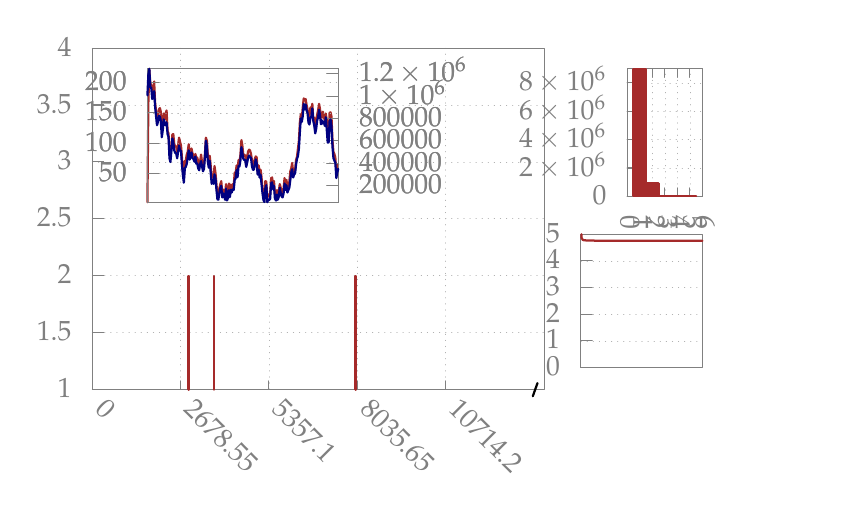
\begin{tikzpicture}[gnuplot, xscale=0.8, yscale=0.6]
%% generated with GNUPLOT 5.2p2 (Lua 5.3; terminal rev. 99, script rev. 102)
%% wo 11 jul 2018 11:33:26 CEST
\path (0.000,0.000) rectangle (12.500,8.750);
\gpcolor{color=gp lt color axes}
\gpsetlinetype{gp lt axes}
\gpsetdashtype{gp dt axes}
\gpsetlinewidth{0.50}
\draw[gp path] (1.012,1.218)--(8.197,1.218);
\gpcolor{rgb color={0.502,0.502,0.502}}
\gpsetlinetype{gp lt border}
\gpsetdashtype{gp dt solid}
\gpsetlinewidth{1.00}
\draw[gp path] (1.012,1.218)--(1.192,1.218);
\node[gp node right] at (0.828,1.218) {$1$};
\gpcolor{color=gp lt color axes}
\gpsetlinetype{gp lt axes}
\gpsetdashtype{gp dt axes}
\gpsetlinewidth{0.50}
\draw[gp path] (1.012,2.422)--(8.197,2.422);
\gpcolor{rgb color={0.502,0.502,0.502}}
\gpsetlinetype{gp lt border}
\gpsetdashtype{gp dt solid}
\gpsetlinewidth{1.00}
\draw[gp path] (1.012,2.422)--(1.192,2.422);
\node[gp node right] at (0.828,2.422) {$1.5$};
\gpcolor{color=gp lt color axes}
\gpsetlinetype{gp lt axes}
\gpsetdashtype{gp dt axes}
\gpsetlinewidth{0.50}
\draw[gp path] (1.012,3.626)--(8.197,3.626);
\gpcolor{rgb color={0.502,0.502,0.502}}
\gpsetlinetype{gp lt border}
\gpsetdashtype{gp dt solid}
\gpsetlinewidth{1.00}
\draw[gp path] (1.012,3.626)--(1.192,3.626);
\node[gp node right] at (0.828,3.626) {$2$};
\gpcolor{color=gp lt color axes}
\gpsetlinetype{gp lt axes}
\gpsetdashtype{gp dt axes}
\gpsetlinewidth{0.50}
\draw[gp path] (1.012,4.830)--(8.197,4.830);
\gpcolor{rgb color={0.502,0.502,0.502}}
\gpsetlinetype{gp lt border}
\gpsetdashtype{gp dt solid}
\gpsetlinewidth{1.00}
\draw[gp path] (1.012,4.830)--(1.192,4.830);
\node[gp node right] at (0.828,4.830) {$2.5$};
\gpcolor{color=gp lt color axes}
\gpsetlinetype{gp lt axes}
\gpsetdashtype{gp dt axes}
\gpsetlinewidth{0.50}
\draw[gp path] (1.012,6.033)--(8.197,6.033);
\gpcolor{rgb color={0.502,0.502,0.502}}
\gpsetlinetype{gp lt border}
\gpsetdashtype{gp dt solid}
\gpsetlinewidth{1.00}
\draw[gp path] (1.012,6.033)--(1.192,6.033);
\node[gp node right] at (0.828,6.033) {$3$};
\gpcolor{color=gp lt color axes}
\gpsetlinetype{gp lt axes}
\gpsetdashtype{gp dt axes}
\gpsetlinewidth{0.50}
\draw[gp path] (1.012,7.237)--(8.197,7.237);
\gpcolor{rgb color={0.502,0.502,0.502}}
\gpsetlinetype{gp lt border}
\gpsetdashtype{gp dt solid}
\gpsetlinewidth{1.00}
\draw[gp path] (1.012,7.237)--(1.192,7.237);
\node[gp node right] at (0.828,7.237) {$3.5$};
\gpcolor{color=gp lt color axes}
\gpsetlinetype{gp lt axes}
\gpsetdashtype{gp dt axes}
\gpsetlinewidth{0.50}
\draw[gp path] (1.012,8.441)--(8.197,8.441);
\gpcolor{rgb color={0.502,0.502,0.502}}
\gpsetlinetype{gp lt border}
\gpsetdashtype{gp dt solid}
\gpsetlinewidth{1.00}
\draw[gp path] (1.012,8.441)--(1.192,8.441);
\node[gp node right] at (0.828,8.441) {$4$};
\gpcolor{color=gp lt color axes}
\gpsetlinetype{gp lt axes}
\gpsetdashtype{gp dt axes}
\gpsetlinewidth{0.50}
\draw[gp path] (1.012,1.218)--(1.012,8.441);
\gpcolor{rgb color={0.502,0.502,0.502}}
\gpsetlinetype{gp lt border}
\gpsetdashtype{gp dt solid}
\gpsetlinewidth{1.00}
\draw[gp path] (1.012,1.218)--(1.012,1.398);
\node[gp node left,rotate=-45] at (1.012,1.034) {$0$};
\gpcolor{color=gp lt color axes}
\gpsetlinetype{gp lt axes}
\gpsetdashtype{gp dt axes}
\gpsetlinewidth{0.50}
\draw[gp path] (2.414,1.218)--(2.414,8.441);
\gpcolor{rgb color={0.502,0.502,0.502}}
\gpsetlinetype{gp lt border}
\gpsetdashtype{gp dt solid}
\gpsetlinewidth{1.00}
\draw[gp path] (2.414,1.218)--(2.414,1.398);
\node[gp node left,rotate=-45] at (2.414,1.034) {$2678.55$};
\gpcolor{color=gp lt color axes}
\gpsetlinetype{gp lt axes}
\gpsetdashtype{gp dt axes}
\gpsetlinewidth{0.50}
\draw[gp path] (3.816,1.218)--(3.816,8.441);
\gpcolor{rgb color={0.502,0.502,0.502}}
\gpsetlinetype{gp lt border}
\gpsetdashtype{gp dt solid}
\gpsetlinewidth{1.00}
\draw[gp path] (3.816,1.218)--(3.816,1.398);
\node[gp node left,rotate=-45] at (3.816,1.034) {$5357.1$};
\gpcolor{color=gp lt color axes}
\gpsetlinetype{gp lt axes}
\gpsetdashtype{gp dt axes}
\gpsetlinewidth{0.50}
\draw[gp path] (5.218,1.218)--(5.218,8.441);
\gpcolor{rgb color={0.502,0.502,0.502}}
\gpsetlinetype{gp lt border}
\gpsetdashtype{gp dt solid}
\gpsetlinewidth{1.00}
\draw[gp path] (5.218,1.218)--(5.218,1.398);
\node[gp node left,rotate=-45] at (5.218,1.034) {$8035.65$};
\gpcolor{color=gp lt color axes}
\gpsetlinetype{gp lt axes}
\gpsetdashtype{gp dt axes}
\gpsetlinewidth{0.50}
\draw[gp path] (6.620,1.218)--(6.620,8.441);
\gpcolor{rgb color={0.502,0.502,0.502}}
\gpsetlinetype{gp lt border}
\gpsetdashtype{gp dt solid}
\gpsetlinewidth{1.00}
\draw[gp path] (6.620,1.218)--(6.620,1.398);
\node[gp node left,rotate=-45] at (6.620,1.034) {$10714.2$};
\gpcolor{color=gp lt color axes}
\gpsetlinetype{gp lt axes}
\gpsetdashtype{gp dt axes}
\gpsetlinewidth{0.50}
% \draw[gp path] (-2147483.648,1.218)--(-2147483.648,8.441);
\gpcolor{rgb color={0.502,0.502,0.502}}
\gpsetlinetype{gp lt border}
\gpsetdashtype{gp dt solid}
\gpsetlinewidth{1.00}
\draw[gp path] (1.012,8.441)--(1.012,1.218)--(8.197,1.218)--(8.197,8.441)--cycle;
\gpcolor{rgb color={0.647,0.165,0.165}}
\gpsetlinewidth{2.00}
\draw[gp path] (2.538,1.218)--(2.538,3.626)--(2.543,3.626)--(2.543,1.218)--cycle;
\draw[gp path] (2.941,1.218)--(2.941,3.626)--(2.946,3.626)--(2.946,1.218)--cycle;
\draw[gp path] (5.191,1.218)--(5.191,3.626)--(5.197,3.626)--(5.197,1.218)--cycle;
\gpcolor{color=gp lt color border}
\draw[gp path](8.005,1.074)--(8.079,1.351);
%% coordinates of the plot area
\gpdefrectangularnode{gp plot 1}{\pgfpoint{1.012cm}{1.218cm}}{\pgfpoint{8.197cm}{8.441cm}}
\gpcolor{color=gp lt color axes}
\gpsetlinetype{gp lt axes}
\gpsetdashtype{gp dt axes}
\gpsetlinewidth{0.50}
\draw[gp path] (1.887,5.793)--(4.916,5.793);
\gpcolor{rgb color={0.502,0.502,0.502}}
\gpsetlinetype{gp lt border}
\gpsetdashtype{gp dt solid}
\gpsetlinewidth{1.00}
\draw[gp path] (1.887,5.793)--(2.067,5.793);
\node[gp node right] at (1.703,5.793) {$50$};
\gpcolor{color=gp lt color axes}
\gpsetlinetype{gp lt axes}
\gpsetdashtype{gp dt axes}
\gpsetlinewidth{0.50}
\draw[gp path] (1.887,6.432)--(4.916,6.432);
\gpcolor{rgb color={0.502,0.502,0.502}}
\gpsetlinetype{gp lt border}
\gpsetdashtype{gp dt solid}
\gpsetlinewidth{1.00}
\draw[gp path] (1.887,6.432)--(2.067,6.432);
\node[gp node right] at (1.703,6.432) {$100$};
\gpcolor{color=gp lt color axes}
\gpsetlinetype{gp lt axes}
\gpsetdashtype{gp dt axes}
\gpsetlinewidth{0.50}
\draw[gp path] (1.887,7.071)--(4.916,7.071);
\gpcolor{rgb color={0.502,0.502,0.502}}
\gpsetlinetype{gp lt border}
\gpsetdashtype{gp dt solid}
\gpsetlinewidth{1.00}
\draw[gp path] (1.887,7.071)--(2.067,7.071);
\node[gp node right] at (1.703,7.071) {$150$};
\gpcolor{color=gp lt color axes}
\gpsetlinetype{gp lt axes}
\gpsetdashtype{gp dt axes}
\gpsetlinewidth{0.50}
\draw[gp path] (1.887,7.710)--(4.916,7.710);
\gpcolor{rgb color={0.502,0.502,0.502}}
\gpsetlinetype{gp lt border}
\gpsetdashtype{gp dt solid}
\gpsetlinewidth{1.00}
\draw[gp path] (1.887,7.710)--(2.067,7.710);
\node[gp node right] at (1.703,7.710) {$200$};
\draw[gp path] (4.916,5.534)--(4.736,5.534);
\node[gp node left] at (5.100,5.534) {$200000$};
\draw[gp path] (4.916,6.007)--(4.736,6.007);
\node[gp node left] at (5.100,6.007) {$400000$};
\draw[gp path] (4.916,6.480)--(4.736,6.480);
\node[gp node left] at (5.100,6.480) {$600000$};
\draw[gp path] (4.916,6.953)--(4.736,6.953);
\node[gp node left] at (5.100,6.953) {$800000$};
\draw[gp path] (4.916,7.426)--(4.736,7.426);
\node[gp node left] at (5.100,7.426) {$1\times10^{6}$};
\draw[gp path] (4.916,7.898)--(4.736,7.898);
\node[gp node left] at (5.100,7.898) {$1.2\times10^{6}$};
\draw[gp path] (1.887,8.004)--(1.887,5.180)--(4.916,5.180)--(4.916,8.004)--cycle;
\gpcolor{rgb color={0.647,0.165,0.165}}
\gpsetlinewidth{2.00}
\draw[gp path] (1.887,5.180)--(1.902,7.288)--(1.917,8.004)--(1.933,7.685)--(1.948,7.672)%
  --(1.963,7.557)--(1.978,7.480)--(1.994,7.736)--(2.009,7.288)--(2.024,7.110)--(2.039,6.956)%
  --(2.054,6.995)--(2.070,7.148)--(2.085,7.173)--(2.100,7.097)--(2.115,6.713)--(2.131,6.816)%
  --(2.146,7.058)--(2.161,6.931)--(2.176,7.058)--(2.191,7.122)--(2.207,6.688)--(2.222,6.637)%
  --(2.237,6.228)--(2.252,6.215)--(2.268,6.343)--(2.283,6.611)--(2.298,6.624)--(2.313,6.407)%
  --(2.328,6.368)--(2.344,6.356)--(2.359,6.228)--(2.374,6.394)--(2.389,6.547)--(2.405,6.458)%
  --(2.420,6.381)--(2.435,6.126)--(2.450,5.844)--(2.465,5.678)--(2.481,6.049)--(2.496,6.062)%
  --(2.511,6.189)--(2.526,6.241)--(2.542,6.407)--(2.557,6.215)--(2.572,6.253)--(2.587,6.317)%
  --(2.602,6.215)--(2.618,6.177)--(2.633,6.074)--(2.648,6.202)--(2.663,6.126)--(2.678,6.126)%
  --(2.694,6.036)--(2.709,5.934)--(2.724,6.049)--(2.739,6.189)--(2.755,6.023)--(2.770,5.959)%
  --(2.785,5.985)--(2.800,6.202)--(2.815,6.547)--(2.831,6.483)--(2.846,6.164)--(2.861,5.985)%
  --(2.876,6.164)--(2.892,5.947)--(2.907,5.691)--(2.922,5.768)--(2.937,5.704)--(2.952,5.947)%
  --(2.968,5.793)--(2.983,5.563)--(2.998,5.346)--(3.013,5.333)--(3.029,5.474)--(3.044,5.563)%
  --(3.059,5.627)--(3.074,5.397)--(3.089,5.448)--(3.105,5.423)--(3.120,5.346)--(3.135,5.563)%
  --(3.150,5.308)--(3.166,5.372)--(3.181,5.576)--(3.196,5.397)--(3.211,5.551)--(3.226,5.474)%
  --(3.242,5.563)--(3.257,5.525)--(3.272,5.806)--(3.287,5.793)--(3.303,5.959)--(3.318,5.832)%
  --(3.333,6.074)--(3.348,6.023)--(3.363,6.177)--(3.379,6.496)--(3.394,6.381)--(3.409,6.177)%
  --(3.424,6.189)--(3.440,6.164)--(3.455,5.959)--(3.470,6.138)--(3.485,6.253)--(3.500,6.292)%
  --(3.516,6.279)--(3.531,6.202)--(3.546,6.074)--(3.561,5.998)--(3.577,5.972)--(3.592,6.100)%
  --(3.607,6.151)--(3.622,6.126)--(3.637,5.819)--(3.653,5.959)--(3.668,5.819)--(3.683,5.870)%
  --(3.698,5.717)--(3.714,5.448)--(3.729,5.308)--(3.744,5.295)--(3.759,5.627)--(3.774,5.614)%
  --(3.790,5.269)--(3.805,5.346)--(3.820,5.333)--(3.835,5.359)--(3.851,5.691)--(3.866,5.704)%
  --(3.881,5.563)--(3.896,5.627)--(3.911,5.372)--(3.927,5.333)--(3.942,5.436)--(3.957,5.321)%
  --(3.972,5.410)--(3.988,5.563)--(4.003,5.487)--(4.018,5.423)--(4.033,5.372)--(4.048,5.461)%
  --(4.064,5.691)--(4.079,5.538)--(4.094,5.653)--(4.109,5.499)--(4.125,5.538)--(4.140,5.614)%
  --(4.155,5.832)--(4.170,5.896)--(4.185,6.011)--(4.201,5.806)--(4.216,5.857)--(4.231,5.844)%
  --(4.246,6.074)--(4.261,6.138)--(4.277,6.317)--(4.292,6.483)--(4.307,6.867)--(4.322,7.046)%
  --(4.338,6.956)--(4.353,7.186)--(4.368,7.378)--(4.383,7.352)--(4.398,7.365)--(4.414,7.237)%
  --(4.429,7.148)--(4.444,6.969)--(4.459,7.007)--(4.475,7.186)--(4.490,7.148)--(4.505,7.263)%
  --(4.520,6.943)--(4.535,6.969)--(4.551,6.739)--(4.566,6.918)--(4.581,7.033)--(4.596,7.122)%
  --(4.612,7.263)--(4.627,7.148)--(4.642,7.007)--(4.657,6.969)--(4.672,7.097)--(4.688,6.995)%
  --(4.703,6.905)--(4.718,7.058)--(4.733,6.931)--(4.749,6.573)--(4.764,6.496)--(4.779,7.071)%
  --(4.794,7.084)--(4.809,6.995)--(4.825,6.483)--(4.840,6.241)--(4.855,6.202)--(4.870,6.126)%
  --(4.886,5.832)--(4.901,5.959)--(4.916,5.985);
%% coordinates of the plot area
\gpdefrectangularnode{gp plot 2}{\pgfpoint{1.887cm}{5.180cm}}{\pgfpoint{4.916cm}{8.004cm}}
\gpcolor{color=gp lt color axes}
\gpsetlinetype{gp lt axes}
\gpsetdashtype{gp dt axes}
\gpsetlinewidth{0.50}
\draw[gp path] (1.887,5.793)--(4.916,5.793);
\gpcolor{rgb color={0.502,0.502,0.502}}
\gpsetlinetype{gp lt border}
\gpsetdashtype{gp dt solid}
\gpsetlinewidth{1.00}
\draw[gp path] (1.887,5.793)--(2.067,5.793);
\node[gp node right] at (1.703,5.793) {$50$};
\gpcolor{color=gp lt color axes}
\gpsetlinetype{gp lt axes}
\gpsetdashtype{gp dt axes}
\gpsetlinewidth{0.50}
\draw[gp path] (1.887,6.432)--(4.916,6.432);
\gpcolor{rgb color={0.502,0.502,0.502}}
\gpsetlinetype{gp lt border}
\gpsetdashtype{gp dt solid}
\gpsetlinewidth{1.00}
\draw[gp path] (1.887,6.432)--(2.067,6.432);
\node[gp node right] at (1.703,6.432) {$100$};
\gpcolor{color=gp lt color axes}
\gpsetlinetype{gp lt axes}
\gpsetdashtype{gp dt axes}
\gpsetlinewidth{0.50}
\draw[gp path] (1.887,7.071)--(4.916,7.071);
\gpcolor{rgb color={0.502,0.502,0.502}}
\gpsetlinetype{gp lt border}
\gpsetdashtype{gp dt solid}
\gpsetlinewidth{1.00}
\draw[gp path] (1.887,7.071)--(2.067,7.071);
\node[gp node right] at (1.703,7.071) {$150$};
\gpcolor{color=gp lt color axes}
\gpsetlinetype{gp lt axes}
\gpsetdashtype{gp dt axes}
\gpsetlinewidth{0.50}
\draw[gp path] (1.887,7.710)--(4.916,7.710);
\gpcolor{rgb color={0.502,0.502,0.502}}
\gpsetlinetype{gp lt border}
\gpsetdashtype{gp dt solid}
\gpsetlinewidth{1.00}
\draw[gp path] (1.887,7.710)--(2.067,7.710);
\node[gp node right] at (1.703,7.710) {$200$};
\draw[gp path] (4.916,5.534)--(4.736,5.534);
\node[gp node left] at (5.100,5.534) {$200000$};
\draw[gp path] (4.916,6.007)--(4.736,6.007);
\node[gp node left] at (5.100,6.007) {$400000$};
\draw[gp path] (4.916,6.480)--(4.736,6.480);
\node[gp node left] at (5.100,6.480) {$600000$};
\draw[gp path] (4.916,6.953)--(4.736,6.953);
\node[gp node left] at (5.100,6.953) {$800000$};
\draw[gp path] (4.916,7.426)--(4.736,7.426);
\node[gp node left] at (5.100,7.426) {$1\times10^{6}$};
\draw[gp path] (4.916,7.898)--(4.736,7.898);
\node[gp node left] at (5.100,7.898) {$1.2\times10^{6}$};
\draw[gp path] (1.887,8.004)--(1.887,5.180)--(4.916,5.180)--(4.916,8.004)--cycle;
\gpcolor{rgb color={0.000,0.000,0.502}}
\gpsetlinewidth{2.00}
\draw[gp path] (1.887,7.443)--(1.902,7.886)--(1.917,8.004)--(1.933,7.608)--(1.948,7.605)%
  --(1.963,7.365)--(1.978,7.418)--(1.994,7.532)--(2.009,7.207)--(2.024,7.000)--(2.039,6.810)%
  --(2.054,6.878)--(2.070,7.008)--(2.085,6.988)--(2.100,6.905)--(2.115,6.555)--(2.131,6.707)%
  --(2.146,6.932)--(2.161,6.864)--(2.176,6.807)--(2.191,6.872)--(2.207,6.623)--(2.222,6.562)%
  --(2.237,6.114)--(2.252,6.030)--(2.268,6.264)--(2.283,6.531)--(2.298,6.442)--(2.313,6.277)%
  --(2.328,6.226)--(2.344,6.210)--(2.359,6.110)--(2.374,6.245)--(2.389,6.379)--(2.405,6.268)%
  --(2.420,6.268)--(2.435,5.969)--(2.450,5.753)--(2.465,5.593)--(2.481,5.898)--(2.496,5.929)%
  --(2.511,5.992)--(2.526,6.116)--(2.542,6.278)--(2.557,6.081)--(2.572,6.150)--(2.587,6.234)%
  --(2.602,6.117)--(2.618,6.091)--(2.633,6.038)--(2.648,6.147)--(2.663,5.995)--(2.678,6.002)%
  --(2.694,5.896)--(2.709,5.857)--(2.724,5.986)--(2.739,6.051)--(2.755,5.929)--(2.770,5.835)%
  --(2.785,5.886)--(2.800,6.130)--(2.815,6.484)--(2.831,6.365)--(2.846,6.033)--(2.861,5.912)%
  --(2.876,6.056)--(2.892,5.797)--(2.907,5.570)--(2.922,5.647)--(2.937,5.569)--(2.952,5.771)%
  --(2.968,5.677)--(2.983,5.441)--(2.998,5.243)--(3.013,5.233)--(3.029,5.377)--(3.044,5.485)%
  --(3.059,5.528)--(3.074,5.281)--(3.089,5.370)--(3.105,5.315)--(3.120,5.231)--(3.135,5.471)%
  --(3.150,5.217)--(3.166,5.268)--(3.181,5.436)--(3.196,5.290)--(3.211,5.442)--(3.226,5.387)%
  --(3.242,5.453)--(3.257,5.441)--(3.272,5.653)--(3.287,5.682)--(3.303,5.860)--(3.318,5.709)%
  --(3.333,5.944)--(3.348,5.937)--(3.363,6.064)--(3.379,6.344)--(3.394,6.223)--(3.409,6.102)%
  --(3.424,6.074)--(3.440,6.076)--(3.455,5.927)--(3.470,6.015)--(3.485,6.120)--(3.500,6.169)%
  --(3.516,6.131)--(3.531,6.124)--(3.546,5.947)--(3.561,5.870)--(3.577,5.867)--(3.592,5.997)%
  --(3.607,6.087)--(3.622,6.003)--(3.637,5.764)--(3.653,5.868)--(3.668,5.701)--(3.683,5.766)%
  --(3.698,5.568)--(3.714,5.369)--(3.729,5.225)--(3.744,5.185)--(3.759,5.473)--(3.774,5.541)%
  --(3.790,5.180)--(3.805,5.243)--(3.820,5.227)--(3.835,5.254)--(3.851,5.582)--(3.866,5.600)%
  --(3.881,5.456)--(3.896,5.529)--(3.911,5.257)--(3.927,5.215)--(3.942,5.342)--(3.957,5.233)%
  --(3.972,5.293)--(3.988,5.487)--(4.003,5.378)--(4.018,5.299)--(4.033,5.282)--(4.048,5.361)%
  --(4.064,5.577)--(4.079,5.439)--(4.094,5.539)--(4.109,5.385)--(4.125,5.439)--(4.140,5.489)%
  --(4.155,5.648)--(4.170,5.813)--(4.185,5.879)--(4.201,5.704)--(4.216,5.770)--(4.231,5.791)%
  --(4.246,5.972)--(4.261,6.096)--(4.277,6.160)--(4.292,6.320)--(4.307,6.660)--(4.322,6.953)%
  --(4.338,6.880)--(4.353,7.005)--(4.368,7.260)--(4.383,7.148)--(4.398,7.248)--(4.414,7.122)%
  --(4.429,7.070)--(4.444,6.861)--(4.459,6.825)--(4.475,6.964)--(4.490,6.995)--(4.505,7.167)%
  --(4.520,6.899)--(4.535,6.811)--(4.551,6.638)--(4.566,6.733)--(4.581,6.905)--(4.596,6.978)%
  --(4.612,7.136)--(4.627,7.011)--(4.642,6.830)--(4.657,6.913)--(4.672,6.847)--(4.688,6.885)%
  --(4.703,6.795)--(4.718,6.979)--(4.733,6.733)--(4.749,6.443)--(4.764,6.448)--(4.779,6.891)%
  --(4.794,6.931)--(4.809,6.794)--(4.825,6.348)--(4.840,6.113)--(4.855,6.062)--(4.870,6.018)%
  --(4.886,5.690)--(4.901,5.809)--(4.916,5.887);
\gpcolor{color=gp lt color axes}
\gpsetlinetype{gp lt axes}
\gpsetdashtype{gp dt axes}
\gpsetlinewidth{0.50}
\draw[gp path] (9.504,5.304)--(10.697,5.304);
\gpcolor{rgb color={0.502,0.502,0.502}}
\gpsetlinetype{gp lt border}
\gpsetdashtype{gp dt solid}
\gpsetlinewidth{1.00}
\draw[gp path] (9.504,5.304)--(9.684,5.304);
\node[gp node right] at (9.320,5.304) {$0$};
\gpcolor{color=gp lt color axes}
\gpsetlinetype{gp lt axes}
\gpsetdashtype{gp dt axes}
\gpsetlinewidth{0.50}
\draw[gp path] (9.504,5.904)--(10.697,5.904);
\gpcolor{rgb color={0.502,0.502,0.502}}
\gpsetlinetype{gp lt border}
\gpsetdashtype{gp dt solid}
\gpsetlinewidth{1.00}
\draw[gp path] (9.504,5.904)--(9.684,5.904);
\node[gp node right] at (9.320,5.904) {$2\times10^{6}$};
\gpcolor{color=gp lt color axes}
\gpsetlinetype{gp lt axes}
\gpsetdashtype{gp dt axes}
\gpsetlinewidth{0.50}
\draw[gp path] (9.504,6.504)--(10.697,6.504);
\gpcolor{rgb color={0.502,0.502,0.502}}
\gpsetlinetype{gp lt border}
\gpsetdashtype{gp dt solid}
\gpsetlinewidth{1.00}
\draw[gp path] (9.504,6.504)--(9.684,6.504);
\node[gp node right] at (9.320,6.504) {$4\times10^{6}$};
\gpcolor{color=gp lt color axes}
\gpsetlinetype{gp lt axes}
\gpsetdashtype{gp dt axes}
\gpsetlinewidth{0.50}
\draw[gp path] (9.504,7.104)--(10.697,7.104);
\gpcolor{rgb color={0.502,0.502,0.502}}
\gpsetlinetype{gp lt border}
\gpsetdashtype{gp dt solid}
\gpsetlinewidth{1.00}
\draw[gp path] (9.504,7.104)--(9.684,7.104);
\node[gp node right] at (9.320,7.104) {$6\times10^{6}$};
\gpcolor{color=gp lt color axes}
\gpsetlinetype{gp lt axes}
\gpsetdashtype{gp dt axes}
\gpsetlinewidth{0.50}
\draw[gp path] (9.504,7.705)--(10.697,7.705);
\gpcolor{rgb color={0.502,0.502,0.502}}
\gpsetlinetype{gp lt border}
\gpsetdashtype{gp dt solid}
\gpsetlinewidth{1.00}
\draw[gp path] (9.504,7.705)--(9.684,7.705);
\node[gp node right] at (9.320,7.705) {$8\times10^{6}$};
\gpcolor{color=gp lt color axes}
\gpsetlinetype{gp lt axes}
\gpsetdashtype{gp dt axes}
\gpsetlinewidth{0.50}
\draw[gp path] (9.504,5.304)--(9.504,7.824)--(9.504,8.004);
\gpcolor{rgb color={0.502,0.502,0.502}}
\gpsetlinetype{gp lt border}
\gpsetdashtype{gp dt solid}
\gpsetlinewidth{1.00}
\draw[gp path] (9.504,5.304)--(9.504,5.484);
\draw[gp path] (9.504,8.004)--(9.504,7.824);
\node[gp node left,rotate=-90] at (9.504,5.120) {$0$};
\gpcolor{color=gp lt color axes}
\gpsetlinetype{gp lt axes}
\gpsetdashtype{gp dt axes}
\gpsetlinewidth{0.50}
\draw[gp path] (9.703,5.304)--(9.703,7.824)--(9.703,8.004);
\gpcolor{rgb color={0.502,0.502,0.502}}
\gpsetlinetype{gp lt border}
\gpsetdashtype{gp dt solid}
\gpsetlinewidth{1.00}
\draw[gp path] (9.703,5.304)--(9.703,5.484);
\draw[gp path] (9.703,8.004)--(9.703,7.824);
\node[gp node left,rotate=-90] at (9.703,5.120) {$1$};
\gpcolor{color=gp lt color axes}
\gpsetlinetype{gp lt axes}
\gpsetdashtype{gp dt axes}
\gpsetlinewidth{0.50}
\draw[gp path] (9.902,5.304)--(9.902,7.824)--(9.902,8.004);
\gpcolor{rgb color={0.502,0.502,0.502}}
\gpsetlinetype{gp lt border}
\gpsetdashtype{gp dt solid}
\gpsetlinewidth{1.00}
\draw[gp path] (9.902,5.304)--(9.902,5.484);
\draw[gp path] (9.902,8.004)--(9.902,7.824);
\node[gp node left,rotate=-90] at (9.902,5.120) {$2$};
\gpcolor{color=gp lt color axes}
\gpsetlinetype{gp lt axes}
\gpsetdashtype{gp dt axes}
\gpsetlinewidth{0.50}
\draw[gp path] (10.101,5.304)--(10.101,7.824)--(10.101,8.004);
\gpcolor{rgb color={0.502,0.502,0.502}}
\gpsetlinetype{gp lt border}
\gpsetdashtype{gp dt solid}
\gpsetlinewidth{1.00}
\draw[gp path] (10.101,5.304)--(10.101,5.484);
\draw[gp path] (10.101,8.004)--(10.101,7.824);
\node[gp node left,rotate=-90] at (10.101,5.120) {$3$};
\gpcolor{color=gp lt color axes}
\gpsetlinetype{gp lt axes}
\gpsetdashtype{gp dt axes}
\gpsetlinewidth{0.50}
\draw[gp path] (10.299,5.304)--(10.299,7.824)--(10.299,8.004);
\gpcolor{rgb color={0.502,0.502,0.502}}
\gpsetlinetype{gp lt border}
\gpsetdashtype{gp dt solid}
\gpsetlinewidth{1.00}
\draw[gp path] (10.299,5.304)--(10.299,5.484);
\draw[gp path] (10.299,8.004)--(10.299,7.824);
\node[gp node left,rotate=-90] at (10.299,5.120) {$4$};
\gpcolor{color=gp lt color axes}
\gpsetlinetype{gp lt axes}
\gpsetdashtype{gp dt axes}
\gpsetlinewidth{0.50}
\draw[gp path] (10.498,5.304)--(10.498,7.824)--(10.498,8.004);
\gpcolor{rgb color={0.502,0.502,0.502}}
\gpsetlinetype{gp lt border}
\gpsetdashtype{gp dt solid}
\gpsetlinewidth{1.00}
\draw[gp path] (10.498,5.304)--(10.498,5.484);
\draw[gp path] (10.498,8.004)--(10.498,7.824);
\node[gp node left,rotate=-90] at (10.498,5.120) {$5$};
\gpcolor{color=gp lt color axes}
\gpsetlinetype{gp lt axes}
\gpsetdashtype{gp dt axes}
\gpsetlinewidth{0.50}
\draw[gp path] (10.697,5.304)--(10.697,8.004);
\gpcolor{rgb color={0.502,0.502,0.502}}
\gpsetlinetype{gp lt border}
\gpsetdashtype{gp dt solid}
\gpsetlinewidth{1.00}
\draw[gp path] (10.697,5.304)--(10.697,5.484);
\draw[gp path] (10.697,8.004)--(10.697,7.824);
\node[gp node left,rotate=-90] at (10.697,5.120) {$6$};
\draw[gp path] (9.504,8.004)--(9.504,5.304)--(10.697,5.304)--(10.697,8.004)--cycle;
\gpfill{rgb color={0.647,0.165,0.165}} (9.603,5.304)--(9.803,5.304)--(9.803,8.005)--(9.603,8.005)--cycle;
\gpcolor{rgb color={0.647,0.165,0.165}}
\gpsetlinewidth{2.00}
\draw[gp path] (9.603,5.304)--(9.603,8.004)--(9.802,8.004)--(9.802,5.304)--cycle;
\gpfill{rgb color={0.647,0.165,0.165}} (9.802,5.304)--(10.002,5.304)--(10.002,5.578)--(9.802,5.578)--cycle;
\draw[gp path] (9.802,5.304)--(9.802,5.577)--(10.001,5.577)--(10.001,5.304)--cycle;
\gpfill{rgb color={0.647,0.165,0.165}} (10.001,5.304)--(10.201,5.304)--(10.201,5.317)--(10.001,5.317)--cycle;
\draw[gp path] (10.001,5.304)--(10.001,5.316)--(10.200,5.316)--(10.200,5.304)--cycle;
\gpfill{rgb color={0.647,0.165,0.165}} (10.200,5.304)--(10.400,5.304)--(10.400,5.305)--(10.200,5.305)--cycle;
\draw[gp path] (10.200,5.304)--(10.399,5.304)--cycle;
\gpfill{rgb color={0.647,0.165,0.165}} (10.399,5.304)--(10.599,5.304)--(10.599,5.305)--(10.399,5.305)--cycle;
\draw[gp path] (10.399,5.304)--(10.598,5.304)--cycle;
%% coordinates of the plot area
\gpdefrectangularnode{gp plot 3}{\pgfpoint{9.504cm}{5.304cm}}{\pgfpoint{10.697cm}{8.004cm}}
\gpcolor{color=gp lt color axes}
\gpsetlinetype{gp lt axes}
\gpsetdashtype{gp dt axes}
\gpsetlinewidth{0.50}
\draw[gp path] (8.768,1.680)--(10.697,1.680);
\gpcolor{rgb color={0.502,0.502,0.502}}
\gpsetlinetype{gp lt border}
\gpsetdashtype{gp dt solid}
\gpsetlinewidth{1.00}
\draw[gp path] (8.768,1.680)--(8.948,1.680);
\node[gp node right] at (8.584,1.680) {$0$};
\gpcolor{color=gp lt color axes}
\gpsetlinetype{gp lt axes}
\gpsetdashtype{gp dt axes}
\gpsetlinewidth{0.50}
\draw[gp path] (8.768,2.245)--(10.697,2.245);
\gpcolor{rgb color={0.502,0.502,0.502}}
\gpsetlinetype{gp lt border}
\gpsetdashtype{gp dt solid}
\gpsetlinewidth{1.00}
\draw[gp path] (8.768,2.245)--(8.948,2.245);
\node[gp node right] at (8.584,2.245) {$1$};
\gpcolor{color=gp lt color axes}
\gpsetlinetype{gp lt axes}
\gpsetdashtype{gp dt axes}
\gpsetlinewidth{0.50}
\draw[gp path] (8.768,2.810)--(10.697,2.810);
\gpcolor{rgb color={0.502,0.502,0.502}}
\gpsetlinetype{gp lt border}
\gpsetdashtype{gp dt solid}
\gpsetlinewidth{1.00}
\draw[gp path] (8.768,2.810)--(8.948,2.810);
\node[gp node right] at (8.584,2.810) {$2$};
\gpcolor{color=gp lt color axes}
\gpsetlinetype{gp lt axes}
\gpsetdashtype{gp dt axes}
\gpsetlinewidth{0.50}
\draw[gp path] (8.768,3.374)--(10.697,3.374);
\gpcolor{rgb color={0.502,0.502,0.502}}
\gpsetlinetype{gp lt border}
\gpsetdashtype{gp dt solid}
\gpsetlinewidth{1.00}
\draw[gp path] (8.768,3.374)--(8.948,3.374);
\node[gp node right] at (8.584,3.374) {$3$};
\gpcolor{color=gp lt color axes}
\gpsetlinetype{gp lt axes}
\gpsetdashtype{gp dt axes}
\gpsetlinewidth{0.50}
\draw[gp path] (8.768,3.939)--(10.697,3.939);
\gpcolor{rgb color={0.502,0.502,0.502}}
\gpsetlinetype{gp lt border}
\gpsetdashtype{gp dt solid}
\gpsetlinewidth{1.00}
\draw[gp path] (8.768,3.939)--(8.948,3.939);
\node[gp node right] at (8.584,3.939) {$4$};
\gpcolor{color=gp lt color axes}
\gpsetlinetype{gp lt axes}
\gpsetdashtype{gp dt axes}
\gpsetlinewidth{0.50}
\draw[gp path] (8.768,4.504)--(10.697,4.504);
\gpcolor{rgb color={0.502,0.502,0.502}}
\gpsetlinetype{gp lt border}
\gpsetdashtype{gp dt solid}
\gpsetlinewidth{1.00}
\draw[gp path] (8.768,4.504)--(8.948,4.504);
\node[gp node right] at (8.584,4.504) {$5$};
\draw[gp path] (8.768,4.504)--(8.768,1.680)--(10.697,1.680)--(10.697,4.504)--cycle;
\gpcolor{rgb color={0.647,0.165,0.165}}
\gpsetlinewidth{2.00}
\draw[gp path] (8.778,4.504)--(8.778,4.431)--(8.787,4.408)--(8.797,4.385)--(8.807,4.380)%
  --(8.816,4.374)--(8.826,4.374)--(8.836,4.374)--(8.846,4.374)--(8.855,4.368)--(8.865,4.368)%
  --(8.875,4.368)--(8.884,4.368)--(8.894,4.368)--(8.904,4.368)--(8.913,4.368)--(8.923,4.368)%
  --(8.933,4.368)--(8.942,4.368)--(8.952,4.368)--(8.962,4.368)--(8.972,4.368)--(8.981,4.368)%
  --(8.991,4.363)--(9.001,4.363)--(9.010,4.363)--(9.020,4.363)--(9.030,4.363)--(9.039,4.363)%
  --(9.049,4.363)--(9.059,4.363)--(9.068,4.363)--(9.078,4.363)--(9.088,4.363)--(9.098,4.363)%
  --(9.107,4.363)--(9.117,4.363)--(9.127,4.363)--(9.136,4.363)--(9.146,4.363)--(9.156,4.363)%
  --(9.165,4.363)--(9.175,4.363)--(9.185,4.363)--(9.195,4.363)--(9.204,4.363)--(9.214,4.363)%
  --(9.224,4.363)--(9.233,4.363)--(9.243,4.363)--(9.253,4.363)--(9.262,4.363)--(9.272,4.363)%
  --(9.282,4.363)--(9.291,4.363)--(9.301,4.363)--(9.311,4.363)--(9.321,4.363)--(9.330,4.363)%
  --(9.340,4.363)--(9.350,4.363)--(9.359,4.363)--(9.369,4.363)--(9.379,4.363)--(9.388,4.363)%
  --(9.398,4.363)--(9.408,4.363)--(9.417,4.363)--(9.427,4.363)--(9.437,4.363)--(9.447,4.363)%
  --(9.456,4.363)--(9.466,4.363)--(9.476,4.363)--(9.485,4.363)--(9.495,4.363)--(9.505,4.363)%
  --(9.514,4.363)--(9.524,4.363)--(9.534,4.363)--(9.543,4.363)--(9.553,4.363)--(9.563,4.363)%
  --(9.573,4.363)--(9.582,4.363)--(9.592,4.363)--(9.602,4.363)--(9.611,4.363)--(9.621,4.363)%
  --(9.631,4.363)--(9.640,4.363)--(9.650,4.363)--(9.660,4.363)--(9.669,4.363)--(9.679,4.363)%
  --(9.689,4.363)--(9.699,4.363)--(9.708,4.363)--(9.718,4.363)--(9.728,4.363)--(9.737,4.363)%
  --(9.747,4.363)--(9.757,4.363)--(9.766,4.363)--(9.776,4.363)--(9.786,4.363)--(9.796,4.363)%
  --(9.805,4.363)--(9.815,4.363)--(9.825,4.363)--(9.834,4.363)--(9.844,4.363)--(9.854,4.363)%
  --(9.863,4.363)--(9.873,4.363)--(9.883,4.363)--(9.892,4.363)--(9.902,4.363)--(9.912,4.363)%
  --(9.922,4.363)--(9.931,4.363)--(9.941,4.363)--(9.951,4.363)--(9.960,4.363)--(9.970,4.363)%
  --(9.980,4.363)--(9.989,4.363)--(9.999,4.363)--(10.009,4.363)--(10.018,4.363)--(10.028,4.363)%
  --(10.038,4.363)--(10.048,4.363)--(10.057,4.363)--(10.067,4.363)--(10.077,4.363)--(10.086,4.363)%
  --(10.096,4.363)--(10.106,4.363)--(10.115,4.363)--(10.125,4.363)--(10.135,4.363)--(10.144,4.363)%
  --(10.154,4.363)--(10.164,4.363)--(10.174,4.363)--(10.183,4.363)--(10.193,4.363)--(10.203,4.363)%
  --(10.212,4.363)--(10.222,4.363)--(10.232,4.363)--(10.241,4.363)--(10.251,4.363)--(10.261,4.363)%
  --(10.270,4.363)--(10.280,4.363)--(10.290,4.363)--(10.300,4.363)--(10.309,4.363)--(10.319,4.363)%
  --(10.329,4.363)--(10.338,4.363)--(10.348,4.363)--(10.358,4.363)--(10.367,4.363)--(10.377,4.363)%
  --(10.387,4.363)--(10.397,4.363)--(10.406,4.363)--(10.416,4.363)--(10.426,4.363)--(10.435,4.363)%
  --(10.445,4.363)--(10.455,4.363)--(10.464,4.363)--(10.474,4.363)--(10.484,4.363)--(10.493,4.363)%
  --(10.503,4.363)--(10.513,4.363)--(10.523,4.363)--(10.532,4.363)--(10.542,4.363)--(10.552,4.363)%
  --(10.561,4.363)--(10.571,4.363)--(10.581,4.363)--(10.590,4.363)--(10.600,4.363)--(10.610,4.363)%
  --(10.619,4.363)--(10.629,4.363)--(10.639,4.363)--(10.649,4.363)--(10.658,4.363)--(10.668,4.363)%
  --(10.678,4.363)--(10.687,4.363)--(10.697,4.363);
%% coordinates of the plot area
\gpdefrectangularnode{gp plot 4}{\pgfpoint{8.768cm}{1.680cm}}{\pgfpoint{10.697cm}{4.504cm}}
\end{tikzpicture}
%% gnuplot variables
 &
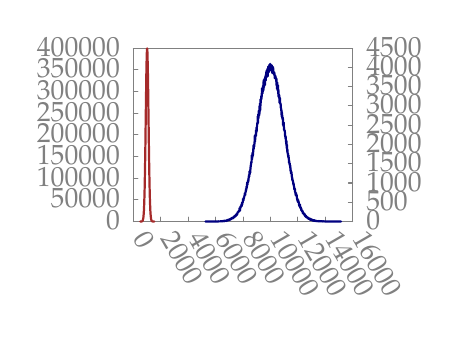
\begin{tikzpicture}[gnuplot, scale=0.3]
%% generated with GNUPLOT 5.2p2 (Lua 5.3; terminal rev. 99, script rev. 102)
%% wo 11 jul 2018 09:51:59 CEST
\path (0.000,0.000) rectangle (12.500,8.750);
\gpcolor{rgb color={0.502,0.502,0.502}}
\gpsetlinetype{gp lt border}
\gpsetdashtype{gp dt solid}
\gpsetlinewidth{1.00}
\draw[gp path] (1.564,1.104)--(1.744,1.104);
\node[gp node right] at (1.380,1.104) {$0$};
\draw[gp path] (1.564,2.021)--(1.744,2.021);
\node[gp node right] at (1.380,2.021) {$50000$};
\draw[gp path] (1.564,2.938)--(1.744,2.938);
\node[gp node right] at (1.380,2.938) {$100000$};
\draw[gp path] (1.564,3.855)--(1.744,3.855);
\node[gp node right] at (1.380,3.855) {$150000$};
\draw[gp path] (1.564,4.773)--(1.744,4.773);
\node[gp node right] at (1.380,4.773) {$200000$};
\draw[gp path] (1.564,5.690)--(1.744,5.690);
\node[gp node right] at (1.380,5.690) {$250000$};
\draw[gp path] (1.564,6.607)--(1.744,6.607);
\node[gp node right] at (1.380,6.607) {$300000$};
\draw[gp path] (1.564,7.524)--(1.744,7.524);
\node[gp node right] at (1.380,7.524) {$350000$};
\draw[gp path] (1.564,8.441)--(1.744,8.441);
\node[gp node right] at (1.380,8.441) {$400000$};
\draw[gp path] (1.564,1.104)--(1.564,1.284);
\node[gp node left,rotate=-60] at (1.564,0.920) {$0$};
\draw[gp path] (2.724,1.104)--(2.724,1.284);
\node[gp node left,rotate=-60] at (2.724,0.920) {$2000$};
\draw[gp path] (3.884,1.104)--(3.884,1.284);
\node[gp node left,rotate=-60] at (3.884,0.920) {$4000$};
\draw[gp path] (5.044,1.104)--(5.044,1.284);
\node[gp node left,rotate=-60] at (5.044,0.920) {$6000$};
\draw[gp path] (6.204,1.104)--(6.204,1.284);
\node[gp node left,rotate=-60] at (6.204,0.920) {$8000$};
\draw[gp path] (7.363,1.104)--(7.363,1.284);
\node[gp node left,rotate=-60] at (7.363,0.920) {$10000$};
\draw[gp path] (8.523,1.104)--(8.523,1.284);
\node[gp node left,rotate=-60] at (8.523,0.920) {$12000$};
\draw[gp path] (9.683,1.104)--(9.683,1.284);
\node[gp node left,rotate=-60] at (9.683,0.920) {$14000$};
\draw[gp path] (10.843,1.104)--(10.843,1.284);
\node[gp node left,rotate=-60] at (10.843,0.920) {$16000$};
\draw[gp path] (10.843,1.104)--(10.663,1.104);
\node[gp node left] at (11.027,1.104) {$0$};
\draw[gp path] (10.843,1.919)--(10.663,1.919);
\node[gp node left] at (11.027,1.919) {$500$};
\draw[gp path] (10.843,2.734)--(10.663,2.734);
\node[gp node left] at (11.027,2.734) {$1000$};
\draw[gp path] (10.843,3.550)--(10.663,3.550);
\node[gp node left] at (11.027,3.550) {$1500$};
\draw[gp path] (10.843,4.365)--(10.663,4.365);
\node[gp node left] at (11.027,4.365) {$2000$};
\draw[gp path] (10.843,5.180)--(10.663,5.180);
\node[gp node left] at (11.027,5.180) {$2500$};
\draw[gp path] (10.843,5.995)--(10.663,5.995);
\node[gp node left] at (11.027,5.995) {$3000$};
\draw[gp path] (10.843,6.811)--(10.663,6.811);
\node[gp node left] at (11.027,6.811) {$3500$};
\draw[gp path] (10.843,7.626)--(10.663,7.626);
\node[gp node left] at (11.027,7.626) {$4000$};
\draw[gp path] (10.843,8.441)--(10.663,8.441);
\node[gp node left] at (11.027,8.441) {$4500$};
\draw[gp path] (1.564,8.441)--(1.564,1.104)--(10.843,1.104)--(10.843,8.441)--cycle;
\gpcolor{rgb color={0.647,0.165,0.165}}
\gpsetlinewidth{2.00}
\draw[gp path] (1.848,1.104)--(1.854,1.104)--(1.860,1.104)--(1.866,1.104)--(1.871,1.104)%
  --(1.877,1.104)--(1.883,1.104)--(1.889,1.104)--(1.895,1.105)--(1.900,1.105)--(1.906,1.106)%
  --(1.912,1.107)--(1.918,1.108)--(1.924,1.110)--(1.929,1.113)--(1.935,1.117)--(1.941,1.122)%
  --(1.947,1.130)--(1.953,1.141)--(1.958,1.155)--(1.964,1.174)--(1.970,1.199)--(1.976,1.232)%
  --(1.982,1.270)--(1.987,1.324)--(1.993,1.387)--(1.999,1.465)--(2.005,1.562)--(2.011,1.679)%
  --(2.016,1.829)--(2.022,1.992)--(2.028,2.186)--(2.034,2.418)--(2.040,2.667)--(2.045,2.966)%
  --(2.051,3.282)--(2.057,3.645)--(2.063,4.017)--(2.069,4.434)--(2.074,4.840)--(2.080,5.298)%
  --(2.086,5.733)--(2.092,6.190)--(2.098,6.595)--(2.103,7.019)--(2.109,7.376)--(2.115,7.688)%
  --(2.121,7.969)--(2.127,8.177)--(2.132,8.329)--(2.138,8.419)--(2.144,8.426)--(2.150,8.350)%
  --(2.156,8.211)--(2.161,7.990)--(2.167,7.718)--(2.173,7.416)--(2.179,7.041)--(2.185,6.661)%
  --(2.190,6.226)--(2.196,5.788)--(2.202,5.329)--(2.208,4.927)--(2.214,4.461)--(2.219,4.068)%
  --(2.225,3.687)--(2.231,3.324)--(2.237,2.992)--(2.243,2.699)--(2.248,2.447)--(2.254,2.208)%
  --(2.260,2.007)--(2.266,1.836)--(2.272,1.702)--(2.277,1.570)--(2.283,1.475)--(2.289,1.395)%
  --(2.295,1.326)--(2.301,1.273)--(2.306,1.232)--(2.312,1.200)--(2.318,1.175)--(2.324,1.155)%
  --(2.330,1.143)--(2.335,1.132)--(2.341,1.124)--(2.347,1.119)--(2.353,1.114)--(2.359,1.110)%
  --(2.364,1.108)--(2.370,1.107)--(2.376,1.106)--(2.382,1.105)--(2.388,1.105)--(2.393,1.105)%
  --(2.399,1.104)--(2.405,1.104)--(2.411,1.104)--(2.417,1.104)--(2.422,1.104)--(2.428,1.104)%
  --(2.434,1.104)--(2.446,1.104);
\gpcolor{rgb color={0.000,0.000,0.502}}
\draw[gp path] (4.614,1.106)--(4.638,1.106)--(4.725,1.106)--(4.759,1.106)--(4.794,1.106)%
  --(4.875,1.106)--(4.893,1.106)--(4.899,1.106)--(4.910,1.106)--(4.928,1.107)--(4.933,1.106)%
  --(4.939,1.106)--(4.945,1.106)--(4.951,1.106)--(4.957,1.107)--(4.968,1.106)--(4.986,1.107)%
  --(4.991,1.106)--(4.997,1.106)--(5.003,1.107)--(5.009,1.106)--(5.015,1.106)--(5.032,1.106)%
  --(5.038,1.107)--(5.044,1.107)--(5.049,1.106)--(5.055,1.106)--(5.061,1.107)--(5.067,1.112)%
  --(5.073,1.109)--(5.090,1.107)--(5.107,1.109)--(5.113,1.106)--(5.119,1.107)--(5.125,1.109)%
  --(5.131,1.111)--(5.136,1.109)--(5.142,1.106)--(5.148,1.107)--(5.154,1.106)--(5.160,1.106)%
  --(5.165,1.114)--(5.171,1.107)--(5.177,1.112)--(5.183,1.109)--(5.189,1.114)--(5.194,1.109)%
  --(5.200,1.111)--(5.206,1.109)--(5.212,1.111)--(5.218,1.115)--(5.223,1.109)--(5.229,1.109)%
  --(5.235,1.109)--(5.241,1.109)--(5.247,1.119)--(5.252,1.114)--(5.258,1.114)--(5.264,1.117)%
  --(5.270,1.115)--(5.276,1.120)--(5.281,1.114)--(5.287,1.114)--(5.293,1.112)--(5.299,1.117)%
  --(5.305,1.119)--(5.310,1.114)--(5.316,1.115)--(5.322,1.117)--(5.328,1.115)--(5.334,1.111)%
  --(5.339,1.112)--(5.345,1.109)--(5.351,1.122)--(5.357,1.115)--(5.363,1.127)--(5.368,1.127)%
  --(5.374,1.124)--(5.380,1.122)--(5.386,1.119)--(5.392,1.133)--(5.397,1.117)--(5.403,1.119)%
  --(5.409,1.122)--(5.415,1.125)--(5.421,1.128)--(5.426,1.115)--(5.432,1.140)--(5.438,1.132)%
  --(5.444,1.132)--(5.450,1.137)--(5.455,1.137)--(5.461,1.138)--(5.467,1.138)--(5.473,1.133)%
  --(5.479,1.140)--(5.484,1.148)--(5.490,1.145)--(5.496,1.125)--(5.502,1.148)--(5.508,1.142)%
  --(5.513,1.148)--(5.519,1.146)--(5.525,1.166)--(5.531,1.135)--(5.537,1.155)--(5.542,1.151)%
  --(5.548,1.159)--(5.554,1.164)--(5.560,1.171)--(5.566,1.164)--(5.571,1.150)--(5.577,1.155)%
  --(5.583,1.158)--(5.589,1.155)--(5.595,1.186)--(5.600,1.163)--(5.606,1.179)--(5.612,1.169)%
  --(5.618,1.192)--(5.624,1.174)--(5.629,1.172)--(5.635,1.197)--(5.641,1.189)--(5.647,1.184)%
  --(5.653,1.174)--(5.658,1.190)--(5.664,1.202)--(5.670,1.189)--(5.676,1.205)--(5.682,1.228)%
  --(5.687,1.208)--(5.693,1.208)--(5.699,1.217)--(5.705,1.231)--(5.711,1.208)--(5.716,1.228)%
  --(5.722,1.226)--(5.728,1.259)--(5.734,1.225)--(5.740,1.236)--(5.745,1.236)--(5.751,1.241)%
  --(5.757,1.267)--(5.763,1.231)--(5.769,1.234)--(5.774,1.247)--(5.780,1.267)--(5.786,1.272)%
  --(5.792,1.243)--(5.798,1.298)--(5.803,1.270)--(5.809,1.288)--(5.815,1.277)--(5.821,1.306)%
  --(5.827,1.314)--(5.832,1.321)--(5.838,1.327)--(5.844,1.298)--(5.850,1.347)--(5.856,1.318)%
  --(5.861,1.345)--(5.867,1.332)--(5.873,1.311)--(5.879,1.331)--(5.885,1.376)--(5.890,1.357)%
  --(5.896,1.358)--(5.902,1.344)--(5.908,1.391)--(5.914,1.381)--(5.919,1.404)--(5.925,1.415)%
  --(5.931,1.401)--(5.937,1.378)--(5.943,1.397)--(5.948,1.437)--(5.954,1.399)--(5.960,1.453)%
  --(5.966,1.479)--(5.972,1.458)--(5.977,1.507)--(5.983,1.472)--(5.989,1.515)--(5.995,1.515)%
  --(6.001,1.503)--(6.006,1.541)--(6.012,1.515)--(6.018,1.525)--(6.024,1.544)--(6.030,1.554)%
  --(6.035,1.559)--(6.041,1.547)--(6.047,1.549)--(6.053,1.655)--(6.059,1.673)--(6.064,1.655)%
  --(6.070,1.557)--(6.076,1.657)--(6.082,1.634)--(6.088,1.662)--(6.093,1.745)--(6.099,1.706)%
  --(6.105,1.748)--(6.111,1.733)--(6.117,1.771)--(6.122,1.750)--(6.128,1.764)--(6.134,1.830)%
  --(6.140,1.738)--(6.146,1.807)--(6.151,1.826)--(6.157,1.834)--(6.163,1.913)--(6.169,1.826)%
  --(6.175,1.896)--(6.180,1.922)--(6.186,1.922)--(6.192,1.919)--(6.198,2.040)--(6.204,2.059)%
  --(6.209,2.012)--(6.215,1.988)--(6.221,2.004)--(6.227,2.058)--(6.232,2.100)--(6.238,2.089)%
  --(6.244,2.130)--(6.250,2.151)--(6.256,2.149)--(6.261,2.206)--(6.267,2.208)--(6.273,2.286)%
  --(6.279,2.275)--(6.285,2.311)--(6.290,2.216)--(6.296,2.301)--(6.302,2.325)--(6.308,2.346)%
  --(6.314,2.374)--(6.319,2.397)--(6.325,2.469)--(6.331,2.482)--(6.337,2.433)--(6.343,2.493)%
  --(6.348,2.580)--(6.354,2.553)--(6.360,2.531)--(6.366,2.593)--(6.372,2.694)--(6.377,2.734)%
  --(6.383,2.754)--(6.389,2.663)--(6.395,2.747)--(6.401,2.752)--(6.406,2.805)--(6.412,2.793)%
  --(6.418,2.863)--(6.424,2.782)--(6.430,2.858)--(6.435,2.919)--(6.441,2.963)--(6.447,2.997)%
  --(6.453,3.075)--(6.459,3.075)--(6.464,2.995)--(6.470,3.090)--(6.476,3.227)--(6.482,3.101)%
  --(6.488,3.193)--(6.493,3.240)--(6.499,3.224)--(6.505,3.170)--(6.511,3.292)--(6.517,3.349)%
  --(6.522,3.411)--(6.528,3.453)--(6.534,3.491)--(6.540,3.525)--(6.546,3.603)--(6.551,3.618)%
  --(6.557,3.628)--(6.563,3.589)--(6.569,3.902)--(6.575,3.724)--(6.580,3.744)--(6.586,3.812)%
  --(6.592,3.796)--(6.598,3.861)--(6.604,4.013)--(6.609,3.907)--(6.615,3.882)--(6.621,3.936)%
  --(6.627,4.009)--(6.633,4.093)--(6.638,4.187)--(6.644,4.270)--(6.650,4.337)--(6.656,4.171)%
  --(6.662,4.363)--(6.667,4.363)--(6.673,4.278)--(6.679,4.345)--(6.685,4.415)--(6.691,4.471)%
  --(6.696,4.730)--(6.702,4.588)--(6.708,4.479)--(6.714,4.663)--(6.720,4.575)--(6.725,4.715)%
  --(6.731,4.786)--(6.737,4.781)--(6.743,4.720)--(6.749,4.748)--(6.754,4.973)--(6.760,4.854)%
  --(6.766,4.937)--(6.772,5.079)--(6.778,4.926)--(6.783,4.975)--(6.789,5.152)--(6.795,5.115)%
  --(6.801,5.258)--(6.807,5.273)--(6.812,5.240)--(6.818,5.283)--(6.824,5.557)--(6.830,5.293)%
  --(6.836,5.284)--(6.841,5.568)--(6.847,5.646)--(6.853,5.534)--(6.859,5.474)--(6.865,5.792)%
  --(6.870,5.705)--(6.876,5.699)--(6.882,5.586)--(6.888,5.717)--(6.894,5.673)--(6.899,5.989)%
  --(6.905,5.881)--(6.911,5.772)--(6.917,6.072)--(6.923,6.100)--(6.928,5.826)--(6.934,5.847)%
  --(6.940,6.279)--(6.946,6.158)--(6.952,6.131)--(6.957,6.261)--(6.963,6.253)--(6.969,6.273)%
  --(6.975,6.416)--(6.981,6.312)--(6.986,6.405)--(6.992,6.390)--(6.998,6.537)--(7.004,6.745)%
  --(7.010,6.680)--(7.015,6.564)--(7.021,6.731)--(7.027,6.520)--(7.033,6.623)--(7.039,6.693)%
  --(7.044,6.657)--(7.050,6.850)--(7.056,6.639)--(7.062,6.784)--(7.068,6.696)--(7.073,7.089)%
  --(7.079,6.895)--(7.085,6.789)--(7.091,6.812)--(7.097,7.037)--(7.102,6.848)--(7.108,7.070)%
  --(7.114,7.062)--(7.120,7.169)--(7.126,7.146)--(7.131,6.879)--(7.137,7.192)--(7.143,7.226)%
  --(7.149,7.161)--(7.155,7.122)--(7.160,7.301)--(7.166,7.071)--(7.172,7.301)--(7.178,7.321)%
  --(7.184,7.194)--(7.189,7.448)--(7.195,7.445)--(7.201,7.267)--(7.207,7.510)--(7.213,7.430)%
  --(7.218,7.319)--(7.224,7.453)--(7.230,7.334)--(7.236,7.521)--(7.242,7.574)--(7.247,7.249)%
  --(7.253,7.451)--(7.259,7.461)--(7.265,7.458)--(7.271,7.667)--(7.276,7.463)--(7.282,7.609)%
  --(7.288,7.541)--(7.294,7.552)--(7.300,7.432)--(7.305,7.626)--(7.311,7.544)--(7.317,7.725)%
  --(7.323,7.732)--(7.329,7.559)--(7.334,7.538)--(7.340,7.528)--(7.346,7.619)--(7.352,7.777)%
  --(7.358,7.546)--(7.363,7.614)--(7.369,7.745)--(7.375,7.616)--(7.381,7.549)--(7.387,7.605)%
  --(7.392,7.578)--(7.398,7.494)--(7.404,7.518)--(7.410,7.546)--(7.416,7.623)--(7.421,7.715)%
  --(7.427,7.494)--(7.433,7.608)--(7.439,7.389)--(7.445,7.608)--(7.450,7.533)--(7.456,7.507)%
  --(7.462,7.544)--(7.468,7.433)--(7.474,7.642)--(7.479,7.500)--(7.485,7.450)--(7.491,7.381)%
  --(7.497,7.393)--(7.503,7.442)--(7.508,7.381)--(7.514,7.329)--(7.520,7.342)--(7.526,7.422)%
  --(7.532,7.323)--(7.537,7.290)--(7.543,7.166)--(7.549,7.301)--(7.555,7.220)--(7.561,7.267)%
  --(7.566,7.277)--(7.572,7.254)--(7.578,7.143)--(7.584,7.190)--(7.590,7.169)--(7.595,7.140)%
  --(7.601,7.132)--(7.607,7.036)--(7.613,7.164)--(7.619,6.879)--(7.624,6.972)--(7.630,6.978)%
  --(7.636,6.713)--(7.642,6.918)--(7.648,6.985)--(7.653,6.739)--(7.659,6.832)--(7.665,6.809)%
  --(7.671,6.638)--(7.677,6.695)--(7.682,6.873)--(7.688,6.690)--(7.694,6.514)--(7.700,6.654)%
  --(7.706,6.396)--(7.711,6.409)--(7.717,6.406)--(7.723,6.331)--(7.729,6.473)--(7.735,6.348)%
  --(7.740,6.396)--(7.746,6.124)--(7.752,6.253)--(7.758,6.333)--(7.764,6.317)--(7.769,6.175)%
  --(7.775,6.101)--(7.781,6.083)--(7.787,6.106)--(7.793,6.065)--(7.798,5.969)--(7.804,5.898)%
  --(7.810,5.909)--(7.816,5.850)--(7.822,5.787)--(7.827,5.813)--(7.833,5.637)--(7.839,5.553)%
  --(7.845,5.749)--(7.851,5.553)--(7.856,5.612)--(7.862,5.560)--(7.868,5.433)--(7.874,5.503)%
  --(7.880,5.506)--(7.885,5.464)--(7.891,5.443)--(7.897,5.188)--(7.903,5.280)--(7.909,5.262)%
  --(7.914,5.247)--(7.920,5.115)--(7.926,5.293)--(7.932,5.068)--(7.938,4.973)--(7.943,5.012)%
  --(7.949,4.967)--(7.955,4.958)--(7.961,4.953)--(7.967,4.952)--(7.972,4.900)--(7.978,4.777)%
  --(7.984,4.735)--(7.990,4.746)--(7.996,4.626)--(8.001,4.699)--(8.007,4.678)--(8.013,4.593)%
  --(8.019,4.502)--(8.025,4.464)--(8.030,4.386)--(8.036,4.404)--(8.042,4.515)--(8.048,4.207)%
  --(8.054,4.278)--(8.059,4.349)--(8.065,4.283)--(8.071,4.106)--(8.077,4.068)--(8.082,4.143)%
  --(8.088,4.013)--(8.094,3.969)--(8.100,3.998)--(8.106,3.944)--(8.111,3.869)--(8.117,3.824)%
  --(8.123,3.902)--(8.129,3.881)--(8.135,3.780)--(8.140,3.742)--(8.146,3.700)--(8.152,3.584)%
  --(8.158,3.665)--(8.164,3.564)--(8.169,3.527)--(8.175,3.572)--(8.181,3.507)--(8.187,3.489)%
  --(8.193,3.447)--(8.198,3.476)--(8.204,3.362)--(8.210,3.374)--(8.216,3.224)--(8.222,3.269)%
  --(8.227,3.250)--(8.233,3.134)--(8.239,3.147)--(8.245,3.129)--(8.251,3.199)--(8.256,3.116)%
  --(8.262,3.092)--(8.268,3.000)--(8.274,2.990)--(8.280,2.945)--(8.285,2.946)--(8.291,2.832)%
  --(8.297,2.899)--(8.303,2.826)--(8.309,2.840)--(8.314,2.805)--(8.320,2.783)--(8.326,2.739)%
  --(8.332,2.681)--(8.338,2.708)--(8.343,2.633)--(8.349,2.695)--(8.355,2.586)--(8.361,2.581)%
  --(8.367,2.555)--(8.372,2.480)--(8.378,2.456)--(8.384,2.503)--(8.390,2.480)--(8.396,2.490)%
  --(8.401,2.363)--(8.407,2.361)--(8.413,2.355)--(8.419,2.306)--(8.425,2.255)--(8.430,2.262)%
  --(8.436,2.209)--(8.442,2.315)--(8.448,2.244)--(8.454,2.265)--(8.459,2.195)--(8.465,2.214)%
  --(8.471,2.151)--(8.477,2.226)--(8.483,2.064)--(8.488,2.066)--(8.494,2.086)--(8.500,2.014)%
  --(8.506,2.050)--(8.512,1.965)--(8.517,2.035)--(8.523,1.924)--(8.529,1.953)--(8.535,1.980)%
  --(8.541,2.009)--(8.546,1.934)--(8.552,1.896)--(8.558,1.934)--(8.564,1.893)--(8.570,1.823)%
  --(8.575,1.807)--(8.581,1.782)--(8.587,1.755)--(8.593,1.756)--(8.599,1.746)--(8.604,1.730)%
  --(8.610,1.821)--(8.616,1.740)--(8.622,1.694)--(8.628,1.681)--(8.633,1.697)--(8.639,1.717)%
  --(8.645,1.668)--(8.651,1.650)--(8.657,1.660)--(8.662,1.663)--(8.668,1.577)--(8.674,1.587)%
  --(8.680,1.565)--(8.686,1.590)--(8.691,1.547)--(8.697,1.551)--(8.703,1.574)--(8.709,1.551)%
  --(8.715,1.546)--(8.720,1.544)--(8.726,1.518)--(8.732,1.455)--(8.738,1.469)--(8.744,1.453)%
  --(8.749,1.445)--(8.755,1.430)--(8.761,1.455)--(8.767,1.459)--(8.773,1.424)--(8.778,1.443)%
  --(8.784,1.399)--(8.790,1.409)--(8.796,1.386)--(8.802,1.391)--(8.807,1.409)--(8.813,1.388)%
  --(8.819,1.414)--(8.825,1.339)--(8.831,1.362)--(8.836,1.313)--(8.842,1.355)--(8.848,1.336)%
  --(8.854,1.345)--(8.860,1.329)--(8.865,1.324)--(8.871,1.344)--(8.877,1.292)--(8.883,1.300)%
  --(8.889,1.272)--(8.894,1.290)--(8.900,1.300)--(8.906,1.270)--(8.912,1.269)--(8.918,1.264)%
  --(8.923,1.288)--(8.929,1.257)--(8.935,1.270)--(8.941,1.270)--(8.947,1.256)--(8.952,1.264)%
  --(8.958,1.270)--(8.964,1.228)--(8.970,1.215)--(8.976,1.230)--(8.981,1.244)--(8.987,1.236)%
  --(8.993,1.234)--(8.999,1.221)--(9.005,1.200)--(9.010,1.217)--(9.016,1.220)--(9.022,1.220)%
  --(9.028,1.213)--(9.034,1.223)--(9.039,1.221)--(9.045,1.179)--(9.051,1.190)--(9.057,1.174)%
  --(9.063,1.205)--(9.068,1.189)--(9.074,1.190)--(9.080,1.203)--(9.086,1.207)--(9.092,1.199)%
  --(9.097,1.177)--(9.103,1.189)--(9.109,1.174)--(9.115,1.166)--(9.121,1.156)--(9.126,1.155)%
  --(9.132,1.174)--(9.138,1.171)--(9.144,1.171)--(9.150,1.150)--(9.155,1.138)--(9.161,1.159)%
  --(9.167,1.151)--(9.173,1.138)--(9.179,1.151)--(9.184,1.150)--(9.190,1.159)--(9.196,1.145)%
  --(9.202,1.142)--(9.208,1.155)--(9.213,1.161)--(9.219,1.138)--(9.225,1.128)--(9.231,1.135)%
  --(9.237,1.140)--(9.242,1.146)--(9.248,1.133)--(9.254,1.137)--(9.260,1.143)--(9.266,1.145)%
  --(9.271,1.130)--(9.277,1.138)--(9.283,1.125)--(9.289,1.120)--(9.295,1.130)--(9.300,1.130)%
  --(9.306,1.128)--(9.312,1.124)--(9.318,1.122)--(9.324,1.119)--(9.329,1.127)--(9.335,1.115)%
  --(9.341,1.120)--(9.347,1.122)--(9.353,1.119)--(9.358,1.120)--(9.364,1.124)--(9.370,1.120)%
  --(9.376,1.115)--(9.382,1.124)--(9.387,1.112)--(9.393,1.117)--(9.399,1.120)--(9.405,1.112)%
  --(9.411,1.119)--(9.416,1.117)--(9.422,1.114)--(9.428,1.112)--(9.434,1.112)--(9.440,1.115)%
  --(9.445,1.112)--(9.451,1.120)--(9.457,1.109)--(9.463,1.112)--(9.469,1.109)--(9.474,1.112)%
  --(9.480,1.117)--(9.486,1.109)--(9.492,1.112)--(9.498,1.119)--(9.509,1.112)--(9.515,1.109)%
  --(9.521,1.109)--(9.527,1.106)--(9.532,1.109)--(9.538,1.107)--(9.544,1.112)--(9.550,1.114)%
  --(9.556,1.111)--(9.567,1.106)--(9.573,1.109)--(9.579,1.107)--(9.585,1.107)--(9.590,1.107)%
  --(9.596,1.106)--(9.602,1.111)--(9.614,1.109)--(9.619,1.115)--(9.625,1.109)--(9.631,1.109)%
  --(9.637,1.106)--(9.643,1.109)--(9.648,1.106)--(9.654,1.109)--(9.666,1.107)--(9.672,1.106)%
  --(9.677,1.107)--(9.683,1.106)--(9.706,1.106)--(9.712,1.106)--(9.724,1.109)--(9.730,1.106)%
  --(9.735,1.107)--(9.741,1.106)--(9.753,1.106)--(9.764,1.106)--(9.770,1.106)--(9.776,1.106)%
  --(9.788,1.106)--(9.799,1.106)--(9.805,1.106)--(9.828,1.106)--(9.869,1.106)--(9.875,1.106)%
  --(9.880,1.106)--(9.932,1.106)--(10.101,1.106)--(10.350,1.106);
%% coordinates of the plot area
\gpdefrectangularnode{gp plot 1}{\pgfpoint{1.564cm}{1.104cm}}{\pgfpoint{10.843cm}{8.441cm}}
\end{tikzpicture}
%% gnuplot variables

\end{tabular}
\end{center}
\caption{\label{fig:inputselection:normal_1to10_randomOn}
  \texttt{Random-Improve}, 1:10 deposit:payment ratio, deposits and
  payments drawn from a normal distribution with mean 10k and 1k, respectively.
  1M cycles.
}
\end{figure}

\begin{figure}[p]
\begin{center}
\scriptsize
\begin{tabular}{l}
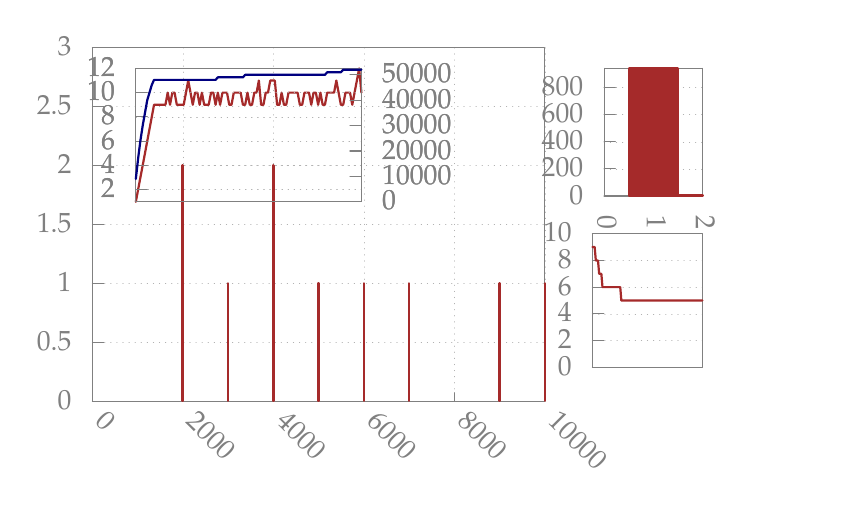
\begin{tikzpicture}[gnuplot, xscale=0.8, yscale=0.6]
%% generated with GNUPLOT 5.2p2 (Lua 5.3; terminal rev. 99, script rev. 102)
%% wo 11 jul 2018 11:38:06 CEST
\path (0.000,0.000) rectangle (12.500,8.750);
\gpcolor{color=gp lt color axes}
\gpsetlinetype{gp lt axes}
\gpsetdashtype{gp dt axes}
\gpsetlinewidth{0.50}
\draw[gp path] (1.012,0.958)--(8.197,0.958);
\gpcolor{rgb color={0.502,0.502,0.502}}
\gpsetlinetype{gp lt border}
\gpsetdashtype{gp dt solid}
\gpsetlinewidth{1.00}
\draw[gp path] (1.012,0.958)--(1.192,0.958);
\node[gp node right] at (0.828,0.958) {$0$};
\gpcolor{color=gp lt color axes}
\gpsetlinetype{gp lt axes}
\gpsetdashtype{gp dt axes}
\gpsetlinewidth{0.50}
\draw[gp path] (1.012,2.205)--(8.197,2.205);
\gpcolor{rgb color={0.502,0.502,0.502}}
\gpsetlinetype{gp lt border}
\gpsetdashtype{gp dt solid}
\gpsetlinewidth{1.00}
\draw[gp path] (1.012,2.205)--(1.192,2.205);
\node[gp node right] at (0.828,2.205) {$0.5$};
\gpcolor{color=gp lt color axes}
\gpsetlinetype{gp lt axes}
\gpsetdashtype{gp dt axes}
\gpsetlinewidth{0.50}
\draw[gp path] (1.012,3.452)--(8.197,3.452);
\gpcolor{rgb color={0.502,0.502,0.502}}
\gpsetlinetype{gp lt border}
\gpsetdashtype{gp dt solid}
\gpsetlinewidth{1.00}
\draw[gp path] (1.012,3.452)--(1.192,3.452);
\node[gp node right] at (0.828,3.452) {$1$};
\gpcolor{color=gp lt color axes}
\gpsetlinetype{gp lt axes}
\gpsetdashtype{gp dt axes}
\gpsetlinewidth{0.50}
\draw[gp path] (1.012,4.700)--(8.197,4.700);
\gpcolor{rgb color={0.502,0.502,0.502}}
\gpsetlinetype{gp lt border}
\gpsetdashtype{gp dt solid}
\gpsetlinewidth{1.00}
\draw[gp path] (1.012,4.700)--(1.192,4.700);
\node[gp node right] at (0.828,4.700) {$1.5$};
\gpcolor{color=gp lt color axes}
\gpsetlinetype{gp lt axes}
\gpsetdashtype{gp dt axes}
\gpsetlinewidth{0.50}
\draw[gp path] (1.012,5.947)--(8.197,5.947);
\gpcolor{rgb color={0.502,0.502,0.502}}
\gpsetlinetype{gp lt border}
\gpsetdashtype{gp dt solid}
\gpsetlinewidth{1.00}
\draw[gp path] (1.012,5.947)--(1.192,5.947);
\node[gp node right] at (0.828,5.947) {$2$};
\gpcolor{color=gp lt color axes}
\gpsetlinetype{gp lt axes}
\gpsetdashtype{gp dt axes}
\gpsetlinewidth{0.50}
\draw[gp path] (1.012,7.194)--(8.197,7.194);
\gpcolor{rgb color={0.502,0.502,0.502}}
\gpsetlinetype{gp lt border}
\gpsetdashtype{gp dt solid}
\gpsetlinewidth{1.00}
\draw[gp path] (1.012,7.194)--(1.192,7.194);
\node[gp node right] at (0.828,7.194) {$2.5$};
\gpcolor{color=gp lt color axes}
\gpsetlinetype{gp lt axes}
\gpsetdashtype{gp dt axes}
\gpsetlinewidth{0.50}
\draw[gp path] (1.012,8.441)--(8.197,8.441);
\gpcolor{rgb color={0.502,0.502,0.502}}
\gpsetlinetype{gp lt border}
\gpsetdashtype{gp dt solid}
\gpsetlinewidth{1.00}
\draw[gp path] (1.012,8.441)--(1.192,8.441);
\node[gp node right] at (0.828,8.441) {$3$};
\gpcolor{color=gp lt color axes}
\gpsetlinetype{gp lt axes}
\gpsetdashtype{gp dt axes}
\gpsetlinewidth{0.50}
\draw[gp path] (1.012,0.958)--(1.012,8.441);
\gpcolor{rgb color={0.502,0.502,0.502}}
\gpsetlinetype{gp lt border}
\gpsetdashtype{gp dt solid}
\gpsetlinewidth{1.00}
\draw[gp path] (1.012,0.958)--(1.012,1.138);
\node[gp node left,rotate=-45] at (1.012,0.774) {$0$};
\gpcolor{color=gp lt color axes}
\gpsetlinetype{gp lt axes}
\gpsetdashtype{gp dt axes}
\gpsetlinewidth{0.50}
\draw[gp path] (2.449,0.958)--(2.449,8.441);
\gpcolor{rgb color={0.502,0.502,0.502}}
\gpsetlinetype{gp lt border}
\gpsetdashtype{gp dt solid}
\gpsetlinewidth{1.00}
\draw[gp path] (2.449,0.958)--(2.449,1.138);
\node[gp node left,rotate=-45] at (2.449,0.774) {$2000$};
\gpcolor{color=gp lt color axes}
\gpsetlinetype{gp lt axes}
\gpsetdashtype{gp dt axes}
\gpsetlinewidth{0.50}
\draw[gp path] (3.886,0.958)--(3.886,8.441);
\gpcolor{rgb color={0.502,0.502,0.502}}
\gpsetlinetype{gp lt border}
\gpsetdashtype{gp dt solid}
\gpsetlinewidth{1.00}
\draw[gp path] (3.886,0.958)--(3.886,1.138);
\node[gp node left,rotate=-45] at (3.886,0.774) {$4000$};
\gpcolor{color=gp lt color axes}
\gpsetlinetype{gp lt axes}
\gpsetdashtype{gp dt axes}
\gpsetlinewidth{0.50}
\draw[gp path] (5.323,0.958)--(5.323,8.441);
\gpcolor{rgb color={0.502,0.502,0.502}}
\gpsetlinetype{gp lt border}
\gpsetdashtype{gp dt solid}
\gpsetlinewidth{1.00}
\draw[gp path] (5.323,0.958)--(5.323,1.138);
\node[gp node left,rotate=-45] at (5.323,0.774) {$6000$};
\gpcolor{color=gp lt color axes}
\gpsetlinetype{gp lt axes}
\gpsetdashtype{gp dt axes}
\gpsetlinewidth{0.50}
\draw[gp path] (6.760,0.958)--(6.760,8.261)--(6.760,8.441);
\gpcolor{rgb color={0.502,0.502,0.502}}
\gpsetlinetype{gp lt border}
\gpsetdashtype{gp dt solid}
\gpsetlinewidth{1.00}
\draw[gp path] (6.760,0.958)--(6.760,1.138);
\node[gp node left,rotate=-45] at (6.760,0.774) {$8000$};
\gpcolor{color=gp lt color axes}
\gpsetlinetype{gp lt axes}
\gpsetdashtype{gp dt axes}
\gpsetlinewidth{0.50}
\draw[gp path] (8.197,0.958)--(8.197,8.441);
\gpcolor{rgb color={0.502,0.502,0.502}}
\gpsetlinetype{gp lt border}
\gpsetdashtype{gp dt solid}
\gpsetlinewidth{1.00}
\draw[gp path] (8.197,0.958)--(8.197,1.138);
\node[gp node left,rotate=-45] at (8.197,0.774) {$10000$};
\draw[gp path] (1.012,8.441)--(1.012,0.958)--(8.197,0.958)--(8.197,8.441)--cycle;
\gpcolor{rgb color={0.647,0.165,0.165}}
\gpsetlinewidth{2.00}
\draw[gp path] (2.445,0.958)--(2.445,5.947)--(2.453,5.947)--(2.453,0.958)--cycle;
\draw[gp path] (3.164,0.958)--(3.164,3.452)--(3.171,3.452)--(3.171,0.958)--cycle;
\draw[gp path] (3.882,0.958)--(3.882,5.947)--(3.890,5.947)--(3.890,0.958)--cycle;
\draw[gp path] (4.601,0.958)--(4.601,3.452)--(4.608,3.452)--(4.608,0.958)--cycle;
\draw[gp path] (5.319,0.958)--(5.319,3.452)--(5.327,3.452)--(5.327,0.958)--cycle;
\draw[gp path] (6.038,0.958)--(6.038,3.452)--(6.045,3.452)--(6.045,0.958)--cycle;
\draw[gp path] (7.475,0.958)--(7.475,3.452)--(7.482,3.452)--(7.482,0.958)--cycle;
\draw[gp path] (8.193,0.958)--(8.193,3.452)--(8.197,3.452)--(8.197,0.958)--cycle;
\gpcolor{color=gp lt color border}
%% coordinates of the plot area
\gpdefrectangularnode{gp plot 1}{\pgfpoint{1.012cm}{0.958cm}}{\pgfpoint{8.197cm}{8.441cm}}
\gpcolor{color=gp lt color axes}
\gpsetlinetype{gp lt axes}
\gpsetdashtype{gp dt axes}
\gpsetlinewidth{0.50}
\draw[gp path] (1.703,5.437)--(5.284,5.437);
\gpcolor{rgb color={0.502,0.502,0.502}}
\gpsetlinetype{gp lt border}
\gpsetdashtype{gp dt solid}
\gpsetlinewidth{1.00}
\draw[gp path] (1.703,5.437)--(1.883,5.437);
\node[gp node right] at (1.519,5.437) {$2$};
\gpcolor{color=gp lt color axes}
\gpsetlinetype{gp lt axes}
\gpsetdashtype{gp dt axes}
\gpsetlinewidth{0.50}
\draw[gp path] (1.703,5.950)--(5.284,5.950);
\gpcolor{rgb color={0.502,0.502,0.502}}
\gpsetlinetype{gp lt border}
\gpsetdashtype{gp dt solid}
\gpsetlinewidth{1.00}
\draw[gp path] (1.703,5.950)--(1.883,5.950);
\node[gp node right] at (1.519,5.950) {$4$};
\gpcolor{color=gp lt color axes}
\gpsetlinetype{gp lt axes}
\gpsetdashtype{gp dt axes}
\gpsetlinewidth{0.50}
\draw[gp path] (1.703,6.464)--(5.284,6.464);
\gpcolor{rgb color={0.502,0.502,0.502}}
\gpsetlinetype{gp lt border}
\gpsetdashtype{gp dt solid}
\gpsetlinewidth{1.00}
\draw[gp path] (1.703,6.464)--(1.883,6.464);
\node[gp node right] at (1.519,6.464) {$6$};
\gpcolor{color=gp lt color axes}
\gpsetlinetype{gp lt axes}
\gpsetdashtype{gp dt axes}
\gpsetlinewidth{0.50}
\draw[gp path] (1.703,6.977)--(5.284,6.977);
\gpcolor{rgb color={0.502,0.502,0.502}}
\gpsetlinetype{gp lt border}
\gpsetdashtype{gp dt solid}
\gpsetlinewidth{1.00}
\draw[gp path] (1.703,6.977)--(1.883,6.977);
\node[gp node right] at (1.519,6.977) {$8$};
\gpcolor{color=gp lt color axes}
\gpsetlinetype{gp lt axes}
\gpsetdashtype{gp dt axes}
\gpsetlinewidth{0.50}
\draw[gp path] (1.703,7.491)--(5.284,7.491);
\gpcolor{rgb color={0.502,0.502,0.502}}
\gpsetlinetype{gp lt border}
\gpsetdashtype{gp dt solid}
\gpsetlinewidth{1.00}
\draw[gp path] (1.703,7.491)--(1.883,7.491);
\node[gp node right] at (1.519,7.491) {$10$};
\gpcolor{color=gp lt color axes}
\gpsetlinetype{gp lt axes}
\gpsetdashtype{gp dt axes}
\gpsetlinewidth{0.50}
\draw[gp path] (1.703,8.004)--(5.284,8.004);
\gpcolor{rgb color={0.502,0.502,0.502}}
\gpsetlinetype{gp lt border}
\gpsetdashtype{gp dt solid}
\gpsetlinewidth{1.00}
\draw[gp path] (1.703,8.004)--(1.883,8.004);
\node[gp node right] at (1.519,8.004) {$12$};
\draw[gp path] (5.284,5.180)--(5.104,5.180);
\node[gp node left] at (5.468,5.180) {$0$};
\draw[gp path] (5.284,5.718)--(5.104,5.718);
\node[gp node left] at (5.468,5.718) {$10000$};
\draw[gp path] (5.284,6.255)--(5.104,6.255);
\node[gp node left] at (5.468,6.255) {$20000$};
\draw[gp path] (5.284,6.793)--(5.104,6.793);
\node[gp node left] at (5.468,6.793) {$30000$};
\draw[gp path] (5.284,7.331)--(5.104,7.331);
\node[gp node left] at (5.468,7.331) {$40000$};
\draw[gp path] (5.284,7.868)--(5.104,7.868);
\node[gp node left] at (5.468,7.868) {$50000$};
\draw[gp path] (1.703,8.004)--(1.703,5.180)--(5.284,5.180)--(5.284,8.004)--cycle;
\gpcolor{rgb color={0.647,0.165,0.165}}
\gpsetlinewidth{2.00}
\draw[gp path] (1.703,5.180)--(1.739,5.437)--(1.775,5.693)--(1.812,5.950)--(1.848,6.207)%
  --(1.884,6.464)--(1.920,6.720)--(1.956,6.977)--(1.992,7.234)--(2.029,7.234)--(2.065,7.234)%
  --(2.101,7.234)--(2.137,7.234)--(2.173,7.234)--(2.209,7.491)--(2.246,7.234)--(2.282,7.491)%
  --(2.318,7.491)--(2.354,7.234)--(2.390,7.234)--(2.426,7.234)--(2.463,7.234)--(2.499,7.491)%
  --(2.535,7.747)--(2.571,7.491)--(2.607,7.234)--(2.643,7.491)--(2.680,7.491)--(2.716,7.234)%
  --(2.752,7.491)--(2.788,7.234)--(2.824,7.234)--(2.860,7.234)--(2.897,7.491)--(2.933,7.491)%
  --(2.969,7.234)--(3.005,7.491)--(3.041,7.234)--(3.078,7.491)--(3.114,7.491)--(3.150,7.491)%
  --(3.186,7.234)--(3.222,7.234)--(3.258,7.491)--(3.295,7.491)--(3.331,7.491)--(3.367,7.491)%
  --(3.403,7.234)--(3.439,7.234)--(3.475,7.491)--(3.512,7.234)--(3.548,7.234)--(3.584,7.491)%
  --(3.620,7.491)--(3.656,7.747)--(3.692,7.234)--(3.729,7.234)--(3.765,7.491)--(3.801,7.491)%
  --(3.837,7.747)--(3.873,7.747)--(3.909,7.747)--(3.946,7.234)--(3.982,7.234)--(4.018,7.491)%
  --(4.054,7.234)--(4.090,7.234)--(4.127,7.491)--(4.163,7.491)--(4.199,7.491)--(4.235,7.491)%
  --(4.271,7.491)--(4.307,7.234)--(4.344,7.234)--(4.380,7.491)--(4.416,7.491)--(4.452,7.491)%
  --(4.488,7.234)--(4.524,7.491)--(4.561,7.491)--(4.597,7.234)--(4.633,7.491)--(4.669,7.234)%
  --(4.705,7.234)--(4.741,7.491)--(4.778,7.491)--(4.814,7.491)--(4.850,7.491)--(4.886,7.747)%
  --(4.922,7.491)--(4.958,7.234)--(4.995,7.234)--(5.031,7.491)--(5.067,7.491)--(5.103,7.491)%
  --(5.139,7.234)--(5.175,7.491)--(5.212,7.747)--(5.248,8.004)--(5.284,7.491);
%% coordinates of the plot area
\gpdefrectangularnode{gp plot 2}{\pgfpoint{1.703cm}{5.180cm}}{\pgfpoint{5.284cm}{8.004cm}}
\gpcolor{color=gp lt color axes}
\gpsetlinetype{gp lt axes}
\gpsetdashtype{gp dt axes}
\gpsetlinewidth{0.50}
\draw[gp path] (1.703,5.437)--(5.284,5.437);
\gpcolor{rgb color={0.502,0.502,0.502}}
\gpsetlinetype{gp lt border}
\gpsetdashtype{gp dt solid}
\gpsetlinewidth{1.00}
\draw[gp path] (1.703,5.437)--(1.883,5.437);
\node[gp node right] at (1.519,5.437) {$2$};
\gpcolor{color=gp lt color axes}
\gpsetlinetype{gp lt axes}
\gpsetdashtype{gp dt axes}
\gpsetlinewidth{0.50}
\draw[gp path] (1.703,5.950)--(5.284,5.950);
\gpcolor{rgb color={0.502,0.502,0.502}}
\gpsetlinetype{gp lt border}
\gpsetdashtype{gp dt solid}
\gpsetlinewidth{1.00}
\draw[gp path] (1.703,5.950)--(1.883,5.950);
\node[gp node right] at (1.519,5.950) {$4$};
\gpcolor{color=gp lt color axes}
\gpsetlinetype{gp lt axes}
\gpsetdashtype{gp dt axes}
\gpsetlinewidth{0.50}
\draw[gp path] (1.703,6.464)--(5.284,6.464);
\gpcolor{rgb color={0.502,0.502,0.502}}
\gpsetlinetype{gp lt border}
\gpsetdashtype{gp dt solid}
\gpsetlinewidth{1.00}
\draw[gp path] (1.703,6.464)--(1.883,6.464);
\node[gp node right] at (1.519,6.464) {$6$};
\gpcolor{color=gp lt color axes}
\gpsetlinetype{gp lt axes}
\gpsetdashtype{gp dt axes}
\gpsetlinewidth{0.50}
\draw[gp path] (1.703,6.977)--(5.284,6.977);
\gpcolor{rgb color={0.502,0.502,0.502}}
\gpsetlinetype{gp lt border}
\gpsetdashtype{gp dt solid}
\gpsetlinewidth{1.00}
\draw[gp path] (1.703,6.977)--(1.883,6.977);
\node[gp node right] at (1.519,6.977) {$8$};
\gpcolor{color=gp lt color axes}
\gpsetlinetype{gp lt axes}
\gpsetdashtype{gp dt axes}
\gpsetlinewidth{0.50}
\draw[gp path] (1.703,7.491)--(5.284,7.491);
\gpcolor{rgb color={0.502,0.502,0.502}}
\gpsetlinetype{gp lt border}
\gpsetdashtype{gp dt solid}
\gpsetlinewidth{1.00}
\draw[gp path] (1.703,7.491)--(1.883,7.491);
\node[gp node right] at (1.519,7.491) {$10$};
\gpcolor{color=gp lt color axes}
\gpsetlinetype{gp lt axes}
\gpsetdashtype{gp dt axes}
\gpsetlinewidth{0.50}
\draw[gp path] (1.703,8.004)--(5.284,8.004);
\gpcolor{rgb color={0.502,0.502,0.502}}
\gpsetlinetype{gp lt border}
\gpsetdashtype{gp dt solid}
\gpsetlinewidth{1.00}
\draw[gp path] (1.703,8.004)--(1.883,8.004);
\node[gp node right] at (1.519,8.004) {$12$};
\draw[gp path] (5.284,5.180)--(5.104,5.180);
\node[gp node left] at (5.468,5.180) {$0$};
\draw[gp path] (5.284,5.718)--(5.104,5.718);
\node[gp node left] at (5.468,5.718) {$10000$};
\draw[gp path] (5.284,6.255)--(5.104,6.255);
\node[gp node left] at (5.468,6.255) {$20000$};
\draw[gp path] (5.284,6.793)--(5.104,6.793);
\node[gp node left] at (5.468,6.793) {$30000$};
\draw[gp path] (5.284,7.331)--(5.104,7.331);
\node[gp node left] at (5.468,7.331) {$40000$};
\draw[gp path] (5.284,7.868)--(5.104,7.868);
\node[gp node left] at (5.468,7.868) {$50000$};
\draw[gp path] (1.703,8.004)--(1.703,5.180)--(5.284,5.180)--(5.284,8.004)--cycle;
\gpcolor{rgb color={0.000,0.000,0.502}}
\gpsetlinewidth{2.00}
\draw[gp path] (1.703,5.664)--(1.739,6.094)--(1.775,6.470)--(1.812,6.793)--(1.848,7.062)%
  --(1.884,7.331)--(1.920,7.492)--(1.956,7.653)--(1.992,7.761)--(2.029,7.761)--(2.065,7.761)%
  --(2.101,7.761)--(2.137,7.761)--(2.173,7.761)--(2.209,7.761)--(2.246,7.761)--(2.282,7.761)%
  --(2.318,7.761)--(2.354,7.761)--(2.390,7.761)--(2.426,7.761)--(2.463,7.761)--(2.499,7.761)%
  --(2.535,7.761)--(2.571,7.761)--(2.607,7.761)--(2.643,7.761)--(2.680,7.761)--(2.716,7.761)%
  --(2.752,7.761)--(2.788,7.761)--(2.824,7.761)--(2.860,7.761)--(2.897,7.761)--(2.933,7.761)%
  --(2.969,7.761)--(3.005,7.815)--(3.041,7.815)--(3.078,7.815)--(3.114,7.815)--(3.150,7.815)%
  --(3.186,7.815)--(3.222,7.815)--(3.258,7.815)--(3.295,7.815)--(3.331,7.815)--(3.367,7.815)%
  --(3.403,7.815)--(3.439,7.868)--(3.475,7.868)--(3.512,7.868)--(3.548,7.868)--(3.584,7.868)%
  --(3.620,7.868)--(3.656,7.868)--(3.692,7.868)--(3.729,7.868)--(3.765,7.868)--(3.801,7.868)%
  --(3.837,7.868)--(3.873,7.868)--(3.909,7.868)--(3.946,7.868)--(3.982,7.868)--(4.018,7.868)%
  --(4.054,7.868)--(4.090,7.868)--(4.127,7.868)--(4.163,7.868)--(4.199,7.868)--(4.235,7.868)%
  --(4.271,7.868)--(4.307,7.868)--(4.344,7.868)--(4.380,7.868)--(4.416,7.868)--(4.452,7.868)%
  --(4.488,7.868)--(4.524,7.868)--(4.561,7.868)--(4.597,7.868)--(4.633,7.868)--(4.669,7.868)%
  --(4.705,7.868)--(4.741,7.922)--(4.778,7.922)--(4.814,7.922)--(4.850,7.922)--(4.886,7.922)%
  --(4.922,7.922)--(4.958,7.922)--(4.995,7.976)--(5.031,7.976)--(5.067,7.976)--(5.103,7.976)%
  --(5.139,7.976)--(5.175,7.976)--(5.212,7.976)--(5.248,7.976)--(5.284,7.976);
\gpcolor{color=gp lt color axes}
\gpsetlinetype{gp lt axes}
\gpsetdashtype{gp dt axes}
\gpsetlinewidth{0.50}
\draw[gp path] (9.136,5.304)--(10.697,5.304);
\gpcolor{rgb color={0.502,0.502,0.502}}
\gpsetlinetype{gp lt border}
\gpsetdashtype{gp dt solid}
\gpsetlinewidth{1.00}
\draw[gp path] (9.136,5.304)--(9.316,5.304);
\node[gp node right] at (8.952,5.304) {$0$};
\gpcolor{color=gp lt color axes}
\gpsetlinetype{gp lt axes}
\gpsetdashtype{gp dt axes}
\gpsetlinewidth{0.50}
\draw[gp path] (9.136,5.877)--(10.697,5.877);
\gpcolor{rgb color={0.502,0.502,0.502}}
\gpsetlinetype{gp lt border}
\gpsetdashtype{gp dt solid}
\gpsetlinewidth{1.00}
\draw[gp path] (9.136,5.877)--(9.316,5.877);
\node[gp node right] at (8.952,5.877) {$200$};
\gpcolor{color=gp lt color axes}
\gpsetlinetype{gp lt axes}
\gpsetdashtype{gp dt axes}
\gpsetlinewidth{0.50}
\draw[gp path] (9.136,6.450)--(10.697,6.450);
\gpcolor{rgb color={0.502,0.502,0.502}}
\gpsetlinetype{gp lt border}
\gpsetdashtype{gp dt solid}
\gpsetlinewidth{1.00}
\draw[gp path] (9.136,6.450)--(9.316,6.450);
\node[gp node right] at (8.952,6.450) {$400$};
\gpcolor{color=gp lt color axes}
\gpsetlinetype{gp lt axes}
\gpsetdashtype{gp dt axes}
\gpsetlinewidth{0.50}
\draw[gp path] (9.136,7.024)--(10.697,7.024);
\gpcolor{rgb color={0.502,0.502,0.502}}
\gpsetlinetype{gp lt border}
\gpsetdashtype{gp dt solid}
\gpsetlinewidth{1.00}
\draw[gp path] (9.136,7.024)--(9.316,7.024);
\node[gp node right] at (8.952,7.024) {$600$};
\gpcolor{color=gp lt color axes}
\gpsetlinetype{gp lt axes}
\gpsetdashtype{gp dt axes}
\gpsetlinewidth{0.50}
\draw[gp path] (9.136,7.597)--(10.697,7.597);
\gpcolor{rgb color={0.502,0.502,0.502}}
\gpsetlinetype{gp lt border}
\gpsetdashtype{gp dt solid}
\gpsetlinewidth{1.00}
\draw[gp path] (9.136,7.597)--(9.316,7.597);
\node[gp node right] at (8.952,7.597) {$800$};
\gpcolor{color=gp lt color axes}
\gpsetlinetype{gp lt axes}
\gpsetdashtype{gp dt axes}
\gpsetlinewidth{0.50}
\draw[gp path] (9.136,5.304)--(9.136,8.004);
\gpcolor{rgb color={0.502,0.502,0.502}}
\gpsetlinetype{gp lt border}
\gpsetdashtype{gp dt solid}
\gpsetlinewidth{1.00}
\draw[gp path] (9.136,5.304)--(9.136,5.484);
\draw[gp path] (9.136,8.004)--(9.136,7.824);
\node[gp node left,rotate=-90] at (9.136,5.120) {$0$};
\gpcolor{color=gp lt color axes}
\gpsetlinetype{gp lt axes}
\gpsetdashtype{gp dt axes}
\gpsetlinewidth{0.50}
\draw[gp path] (9.917,5.304)--(9.917,7.824)--(9.917,8.004);
\gpcolor{rgb color={0.502,0.502,0.502}}
\gpsetlinetype{gp lt border}
\gpsetdashtype{gp dt solid}
\gpsetlinewidth{1.00}
\draw[gp path] (9.917,5.304)--(9.917,5.484);
\draw[gp path] (9.917,8.004)--(9.917,7.824);
\node[gp node left,rotate=-90] at (9.917,5.120) {$1$};
\gpcolor{color=gp lt color axes}
\gpsetlinetype{gp lt axes}
\gpsetdashtype{gp dt axes}
\gpsetlinewidth{0.50}
\draw[gp path] (10.697,5.304)--(10.697,8.004);
\gpcolor{rgb color={0.502,0.502,0.502}}
\gpsetlinetype{gp lt border}
\gpsetdashtype{gp dt solid}
\gpsetlinewidth{1.00}
\draw[gp path] (10.697,5.304)--(10.697,5.484);
\draw[gp path] (10.697,8.004)--(10.697,7.824);
\node[gp node left,rotate=-90] at (10.697,5.120) {$2$};
\draw[gp path] (9.136,8.004)--(9.136,5.304)--(10.697,5.304)--(10.697,8.004)--cycle;
\gpfill{rgb color={0.647,0.165,0.165}} (9.526,5.304)--(10.308,5.304)--(10.308,8.005)--(9.526,8.005)--cycle;
\gpcolor{rgb color={0.647,0.165,0.165}}
\gpsetlinewidth{2.00}
\draw[gp path] (9.526,5.304)--(9.526,8.004)--(10.307,8.004)--(10.307,5.304)--cycle;
\gpfill{rgb color={0.647,0.165,0.165}} (10.307,5.304)--(10.698,5.304)--(10.698,5.322)--(10.307,5.322)--cycle;
\draw[gp path] (10.307,5.304)--(10.307,5.321)--(10.697,5.321)--(10.697,5.304)--cycle;
%% coordinates of the plot area
\gpdefrectangularnode{gp plot 3}{\pgfpoint{9.136cm}{5.304cm}}{\pgfpoint{10.697cm}{8.004cm}}
\gpcolor{color=gp lt color axes}
\gpsetlinetype{gp lt axes}
\gpsetdashtype{gp dt axes}
\gpsetlinewidth{0.50}
\draw[gp path] (8.952,1.680)--(10.697,1.680);
\gpcolor{rgb color={0.502,0.502,0.502}}
\gpsetlinetype{gp lt border}
\gpsetdashtype{gp dt solid}
\gpsetlinewidth{1.00}
\draw[gp path] (8.952,1.680)--(9.132,1.680);
\node[gp node right] at (8.768,1.680) {$0$};
\gpcolor{color=gp lt color axes}
\gpsetlinetype{gp lt axes}
\gpsetdashtype{gp dt axes}
\gpsetlinewidth{0.50}
\draw[gp path] (8.952,2.245)--(10.697,2.245);
\gpcolor{rgb color={0.502,0.502,0.502}}
\gpsetlinetype{gp lt border}
\gpsetdashtype{gp dt solid}
\gpsetlinewidth{1.00}
\draw[gp path] (8.952,2.245)--(9.132,2.245);
\node[gp node right] at (8.768,2.245) {$2$};
\gpcolor{color=gp lt color axes}
\gpsetlinetype{gp lt axes}
\gpsetdashtype{gp dt axes}
\gpsetlinewidth{0.50}
\draw[gp path] (8.952,2.810)--(10.697,2.810);
\gpcolor{rgb color={0.502,0.502,0.502}}
\gpsetlinetype{gp lt border}
\gpsetdashtype{gp dt solid}
\gpsetlinewidth{1.00}
\draw[gp path] (8.952,2.810)--(9.132,2.810);
\node[gp node right] at (8.768,2.810) {$4$};
\gpcolor{color=gp lt color axes}
\gpsetlinetype{gp lt axes}
\gpsetdashtype{gp dt axes}
\gpsetlinewidth{0.50}
\draw[gp path] (8.952,3.374)--(10.697,3.374);
\gpcolor{rgb color={0.502,0.502,0.502}}
\gpsetlinetype{gp lt border}
\gpsetdashtype{gp dt solid}
\gpsetlinewidth{1.00}
\draw[gp path] (8.952,3.374)--(9.132,3.374);
\node[gp node right] at (8.768,3.374) {$6$};
\gpcolor{color=gp lt color axes}
\gpsetlinetype{gp lt axes}
\gpsetdashtype{gp dt axes}
\gpsetlinewidth{0.50}
\draw[gp path] (8.952,3.939)--(10.697,3.939);
\gpcolor{rgb color={0.502,0.502,0.502}}
\gpsetlinetype{gp lt border}
\gpsetdashtype{gp dt solid}
\gpsetlinewidth{1.00}
\draw[gp path] (8.952,3.939)--(9.132,3.939);
\node[gp node right] at (8.768,3.939) {$8$};
\gpcolor{color=gp lt color axes}
\gpsetlinetype{gp lt axes}
\gpsetdashtype{gp dt axes}
\gpsetlinewidth{0.50}
\draw[gp path] (8.952,4.504)--(10.697,4.504);
\gpcolor{rgb color={0.502,0.502,0.502}}
\gpsetlinetype{gp lt border}
\gpsetdashtype{gp dt solid}
\gpsetlinewidth{1.00}
\draw[gp path] (8.952,4.504)--(9.132,4.504);
\node[gp node right] at (8.768,4.504) {$10$};
\draw[gp path] (8.952,4.504)--(8.952,1.680)--(10.697,1.680)--(10.697,4.504)--cycle;
\gpcolor{rgb color={0.647,0.165,0.165}}
\gpsetlinewidth{2.00}
\draw[gp path] (8.952,4.222)--(8.970,4.222)--(8.987,4.222)--(9.005,3.939)--(9.023,3.939)%
  --(9.040,3.939)--(9.058,3.657)--(9.075,3.657)--(9.093,3.657)--(9.111,3.374)--(9.128,3.374)%
  --(9.146,3.374)--(9.164,3.374)--(9.181,3.374)--(9.199,3.374)--(9.216,3.374)--(9.234,3.374)%
  --(9.252,3.374)--(9.269,3.374)--(9.287,3.374)--(9.305,3.374)--(9.322,3.374)--(9.340,3.374)%
  --(9.357,3.374)--(9.375,3.374)--(9.393,3.374)--(9.410,3.092)--(9.428,3.092)--(9.446,3.092)%
  --(9.463,3.092)--(9.481,3.092)--(9.498,3.092)--(9.516,3.092)--(9.534,3.092)--(9.551,3.092)%
  --(9.569,3.092)--(9.587,3.092)--(9.604,3.092)--(9.622,3.092)--(9.639,3.092)--(9.657,3.092)%
  --(9.675,3.092)--(9.692,3.092)--(9.710,3.092)--(9.728,3.092)--(9.745,3.092)--(9.763,3.092)%
  --(9.780,3.092)--(9.798,3.092)--(9.816,3.092)--(9.833,3.092)--(9.851,3.092)--(9.869,3.092)%
  --(9.886,3.092)--(9.904,3.092)--(9.921,3.092)--(9.939,3.092)--(9.957,3.092)--(9.974,3.092)%
  --(9.992,3.092)--(10.010,3.092)--(10.027,3.092)--(10.045,3.092)--(10.062,3.092)--(10.080,3.092)%
  --(10.098,3.092)--(10.115,3.092)--(10.133,3.092)--(10.151,3.092)--(10.168,3.092)--(10.186,3.092)%
  --(10.203,3.092)--(10.221,3.092)--(10.239,3.092)--(10.256,3.092)--(10.274,3.092)--(10.292,3.092)%
  --(10.309,3.092)--(10.327,3.092)--(10.344,3.092)--(10.362,3.092)--(10.380,3.092)--(10.397,3.092)%
  --(10.415,3.092)--(10.433,3.092)--(10.450,3.092)--(10.468,3.092)--(10.485,3.092)--(10.503,3.092)%
  --(10.521,3.092)--(10.538,3.092)--(10.556,3.092)--(10.574,3.092)--(10.591,3.092)--(10.609,3.092)%
  --(10.626,3.092)--(10.644,3.092)--(10.662,3.092)--(10.679,3.092)--(10.697,3.092);
%% coordinates of the plot area
\gpdefrectangularnode{gp plot 4}{\pgfpoint{8.952cm}{1.680cm}}{\pgfpoint{10.697cm}{4.504cm}}
\end{tikzpicture}
%% gnuplot variables

\end{tabular}
\end{center}
\caption{\label{fig:inputselection:constant_1to10_randomOn}
  \texttt{Random-Improve}, 1:10 deposit:payment ratio, all deposits exactly
  10k, all payments exactly 1k (no randomness). First 100 cycles only.
}
\end{figure}

We can see this more clearly
when we slow things right down, and remove any source of randomness. Figure~\ref{fig:inputselection:constant_1to10_randomOn} shows the
same 1:10 ratio again, but now only the first 100 cycles, and all deposits
exactly 10k and all payments exactly 1k.
We can see the large value being deposited, and then shifting to the left in the
histogram as it is getting used for deposits, each time decreasing that large
output by 1k. Indeed, this takes 10 slots on average, which makes sense given
the 10:1 ratio; moreover, the \emph{average value} of the ``large output'' in such a
10-slot cycle is 5k, explaining why we are getting 5.0 change:payment ratio.

The algorithm however is \emph{not} creating dust outputs; the 1k change outputs
it is generating \emph{are} getting used, and the size of the UTxO is perfectly
stable. Indeed, back in Figure~\ref{fig:inputselection:normal_1to10_randomOn} we
can see that the size of the UTxO tracks the balance perfectly; moreover, the
vast majority of transactions only use a single input, which is what we'd expect
for a 10:0 deposit:payment ratio.

\subsubsection{Real data}

\paragraph{\texttt{MoneyPot.com}}

Ideally, of course, we run the simulation against \emph{real} event streams from
existing wallets. Unfortunately, such data is hard to come by. Erhardt was able
to find one such dataset, provided by \texttt{MoneyPot.com}
\citep{MoneyPotdataset}. Figure~\ref{fig:inputselection:MoneyPot_randomOn} shows
the results of running our algorithm on this dataset.

\begin{figure}[p]
\begin{center}
\scriptsize
\begin{tabular}{ll}
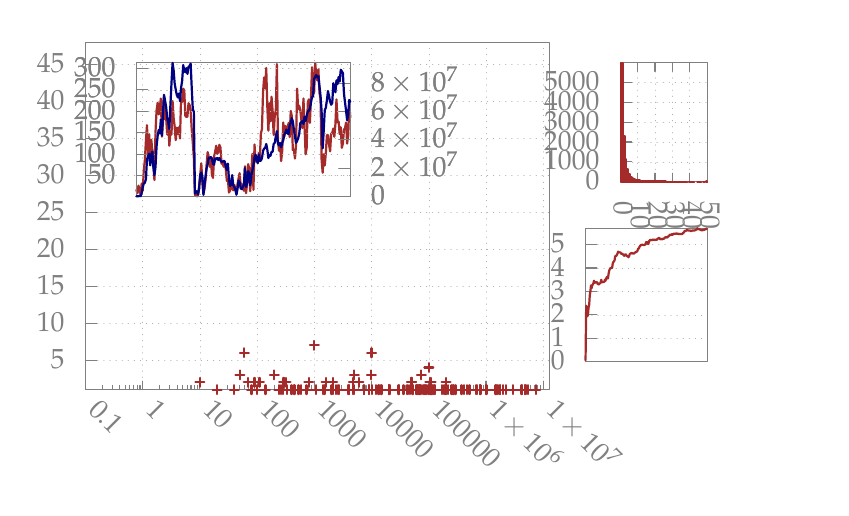
\begin{tikzpicture}[gnuplot, xscale=0.8, yscale=0.6]
%% generated with GNUPLOT 5.2p2 (Lua 5.3; terminal rev. 99, script rev. 102)
%% wo 11 jul 2018 11:48:30 CEST
\path (0.000,0.000) rectangle (12.500,8.750);
\gpcolor{color=gp lt color axes}
\gpsetlinetype{gp lt axes}
\gpsetdashtype{gp dt axes}
\gpsetlinewidth{0.50}
\draw[gp path] (0.828,1.714)--(8.197,1.714);
\gpcolor{rgb color={0.502,0.502,0.502}}
\gpsetlinetype{gp lt border}
\gpsetdashtype{gp dt solid}
\gpsetlinewidth{1.00}
\draw[gp path] (0.828,1.714)--(1.008,1.714);
\node[gp node right] at (0.644,1.714) {$5$};
\gpcolor{color=gp lt color axes}
\gpsetlinetype{gp lt axes}
\gpsetdashtype{gp dt axes}
\gpsetlinewidth{0.50}
\draw[gp path] (0.828,2.496)--(8.197,2.496);
\gpcolor{rgb color={0.502,0.502,0.502}}
\gpsetlinetype{gp lt border}
\gpsetdashtype{gp dt solid}
\gpsetlinewidth{1.00}
\draw[gp path] (0.828,2.496)--(1.008,2.496);
\node[gp node right] at (0.644,2.496) {$10$};
\gpcolor{color=gp lt color axes}
\gpsetlinetype{gp lt axes}
\gpsetdashtype{gp dt axes}
\gpsetlinewidth{0.50}
\draw[gp path] (0.828,3.278)--(8.197,3.278);
\gpcolor{rgb color={0.502,0.502,0.502}}
\gpsetlinetype{gp lt border}
\gpsetdashtype{gp dt solid}
\gpsetlinewidth{1.00}
\draw[gp path] (0.828,3.278)--(1.008,3.278);
\node[gp node right] at (0.644,3.278) {$15$};
\gpcolor{color=gp lt color axes}
\gpsetlinetype{gp lt axes}
\gpsetdashtype{gp dt axes}
\gpsetlinewidth{0.50}
\draw[gp path] (0.828,4.060)--(8.197,4.060);
\gpcolor{rgb color={0.502,0.502,0.502}}
\gpsetlinetype{gp lt border}
\gpsetdashtype{gp dt solid}
\gpsetlinewidth{1.00}
\draw[gp path] (0.828,4.060)--(1.008,4.060);
\node[gp node right] at (0.644,4.060) {$20$};
\gpcolor{color=gp lt color axes}
\gpsetlinetype{gp lt axes}
\gpsetdashtype{gp dt axes}
\gpsetlinewidth{0.50}
\draw[gp path] (0.828,4.843)--(8.197,4.843);
\gpcolor{rgb color={0.502,0.502,0.502}}
\gpsetlinetype{gp lt border}
\gpsetdashtype{gp dt solid}
\gpsetlinewidth{1.00}
\draw[gp path] (0.828,4.843)--(1.008,4.843);
\node[gp node right] at (0.644,4.843) {$25$};
\gpcolor{color=gp lt color axes}
\gpsetlinetype{gp lt axes}
\gpsetdashtype{gp dt axes}
\gpsetlinewidth{0.50}
\draw[gp path] (0.828,5.625)--(8.197,5.625);
\gpcolor{rgb color={0.502,0.502,0.502}}
\gpsetlinetype{gp lt border}
\gpsetdashtype{gp dt solid}
\gpsetlinewidth{1.00}
\draw[gp path] (0.828,5.625)--(1.008,5.625);
\node[gp node right] at (0.644,5.625) {$30$};
\gpcolor{color=gp lt color axes}
\gpsetlinetype{gp lt axes}
\gpsetdashtype{gp dt axes}
\gpsetlinewidth{0.50}
\draw[gp path] (0.828,6.407)--(8.197,6.407);
\gpcolor{rgb color={0.502,0.502,0.502}}
\gpsetlinetype{gp lt border}
\gpsetdashtype{gp dt solid}
\gpsetlinewidth{1.00}
\draw[gp path] (0.828,6.407)--(1.008,6.407);
\node[gp node right] at (0.644,6.407) {$35$};
\gpcolor{color=gp lt color axes}
\gpsetlinetype{gp lt axes}
\gpsetdashtype{gp dt axes}
\gpsetlinewidth{0.50}
\draw[gp path] (0.828,7.189)--(8.197,7.189);
\gpcolor{rgb color={0.502,0.502,0.502}}
\gpsetlinetype{gp lt border}
\gpsetdashtype{gp dt solid}
\gpsetlinewidth{1.00}
\draw[gp path] (0.828,7.189)--(1.008,7.189);
\node[gp node right] at (0.644,7.189) {$40$};
\gpcolor{color=gp lt color axes}
\gpsetlinetype{gp lt axes}
\gpsetdashtype{gp dt axes}
\gpsetlinewidth{0.50}
\draw[gp path] (0.828,7.972)--(8.197,7.972);
\gpcolor{rgb color={0.502,0.502,0.502}}
\gpsetlinetype{gp lt border}
\gpsetdashtype{gp dt solid}
\gpsetlinewidth{1.00}
\draw[gp path] (0.828,7.972)--(1.008,7.972);
\node[gp node right] at (0.644,7.972) {$45$};
\gpcolor{color=gp lt color axes}
\gpsetlinetype{gp lt axes}
\gpsetdashtype{gp dt axes}
\gpsetlinewidth{0.50}
\draw[gp path] (0.828,1.088)--(0.828,8.441);
\gpcolor{rgb color={0.502,0.502,0.502}}
\gpsetlinetype{gp lt border}
\gpsetdashtype{gp dt solid}
\gpsetlinewidth{1.00}
\draw[gp path] (0.828,1.088)--(0.828,1.268);
\node[gp node left,rotate=-45] at (0.828,0.904) {$0.1$};
\draw[gp path] (1.102,1.088)--(1.102,1.178);
\draw[gp path] (1.262,1.088)--(1.262,1.178);
\draw[gp path] (1.375,1.088)--(1.375,1.178);
\draw[gp path] (1.463,1.088)--(1.463,1.178);
\draw[gp path] (1.535,1.088)--(1.535,1.178);
\draw[gp path] (1.596,1.088)--(1.596,1.178);
\draw[gp path] (1.649,1.088)--(1.649,1.178);
\draw[gp path] (1.695,1.088)--(1.695,1.178);
\gpcolor{color=gp lt color axes}
\gpsetlinetype{gp lt axes}
\gpsetdashtype{gp dt axes}
\gpsetlinewidth{0.50}
\draw[gp path] (1.737,1.088)--(1.737,8.441);
\gpcolor{rgb color={0.502,0.502,0.502}}
\gpsetlinetype{gp lt border}
\gpsetdashtype{gp dt solid}
\gpsetlinewidth{1.00}
\draw[gp path] (1.737,1.088)--(1.737,1.268);
\node[gp node left,rotate=-45] at (1.737,0.904) {$1$};
\draw[gp path] (2.010,1.088)--(2.010,1.178);
\draw[gp path] (2.170,1.088)--(2.170,1.178);
\draw[gp path] (2.284,1.088)--(2.284,1.178);
\draw[gp path] (2.372,1.088)--(2.372,1.178);
\draw[gp path] (2.444,1.088)--(2.444,1.178);
\draw[gp path] (2.505,1.088)--(2.505,1.178);
\draw[gp path] (2.557,1.088)--(2.557,1.178);
\draw[gp path] (2.604,1.088)--(2.604,1.178);
\gpcolor{color=gp lt color axes}
\gpsetlinetype{gp lt axes}
\gpsetdashtype{gp dt axes}
\gpsetlinewidth{0.50}
\draw[gp path] (2.645,1.088)--(2.645,8.441);
\gpcolor{rgb color={0.502,0.502,0.502}}
\gpsetlinetype{gp lt border}
\gpsetdashtype{gp dt solid}
\gpsetlinewidth{1.00}
\draw[gp path] (2.645,1.088)--(2.645,1.268);
\node[gp node left,rotate=-45] at (2.645,0.904) {$10$};
\draw[gp path] (2.919,1.088)--(2.919,1.178);
\draw[gp path] (3.079,1.088)--(3.079,1.178);
\draw[gp path] (3.192,1.088)--(3.192,1.178);
\draw[gp path] (3.280,1.088)--(3.280,1.178);
\draw[gp path] (3.352,1.088)--(3.352,1.178);
\draw[gp path] (3.413,1.088)--(3.413,1.178);
\draw[gp path] (3.466,1.088)--(3.466,1.178);
\draw[gp path] (3.512,1.088)--(3.512,1.178);
\gpcolor{color=gp lt color axes}
\gpsetlinetype{gp lt axes}
\gpsetdashtype{gp dt axes}
\gpsetlinewidth{0.50}
\draw[gp path] (3.554,1.088)--(3.554,8.441);
\gpcolor{rgb color={0.502,0.502,0.502}}
\gpsetlinetype{gp lt border}
\gpsetdashtype{gp dt solid}
\gpsetlinewidth{1.00}
\draw[gp path] (3.554,1.088)--(3.554,1.268);
\node[gp node left,rotate=-45] at (3.554,0.904) {$100$};
\draw[gp path] (3.827,1.088)--(3.827,1.178);
\draw[gp path] (3.987,1.088)--(3.987,1.178);
\draw[gp path] (4.101,1.088)--(4.101,1.178);
\draw[gp path] (4.189,1.088)--(4.189,1.178);
\draw[gp path] (4.261,1.088)--(4.261,1.178);
\draw[gp path] (4.322,1.088)--(4.322,1.178);
\draw[gp path] (4.374,1.088)--(4.374,1.178);
\draw[gp path] (4.421,1.088)--(4.421,1.178);
\gpcolor{color=gp lt color axes}
\gpsetlinetype{gp lt axes}
\gpsetdashtype{gp dt axes}
\gpsetlinewidth{0.50}
\draw[gp path] (4.463,1.088)--(4.463,8.441);
\gpcolor{rgb color={0.502,0.502,0.502}}
\gpsetlinetype{gp lt border}
\gpsetdashtype{gp dt solid}
\gpsetlinewidth{1.00}
\draw[gp path] (4.463,1.088)--(4.463,1.268);
\node[gp node left,rotate=-45] at (4.463,0.904) {$1000$};
\draw[gp path] (4.736,1.088)--(4.736,1.178);
\draw[gp path] (4.896,1.088)--(4.896,1.178);
\draw[gp path] (5.010,1.088)--(5.010,1.178);
\draw[gp path] (5.098,1.088)--(5.098,1.178);
\draw[gp path] (5.170,1.088)--(5.170,1.178);
\draw[gp path] (5.230,1.088)--(5.230,1.178);
\draw[gp path] (5.283,1.088)--(5.283,1.178);
\draw[gp path] (5.330,1.088)--(5.330,1.178);
\gpcolor{color=gp lt color axes}
\gpsetlinetype{gp lt axes}
\gpsetdashtype{gp dt axes}
\gpsetlinewidth{0.50}
\draw[gp path] (5.371,1.088)--(5.371,8.441);
\gpcolor{rgb color={0.502,0.502,0.502}}
\gpsetlinetype{gp lt border}
\gpsetdashtype{gp dt solid}
\gpsetlinewidth{1.00}
\draw[gp path] (5.371,1.088)--(5.371,1.268);
\node[gp node left,rotate=-45] at (5.371,0.904) {$10000$};
\draw[gp path] (5.645,1.088)--(5.645,1.178);
\draw[gp path] (5.805,1.088)--(5.805,1.178);
\draw[gp path] (5.918,1.088)--(5.918,1.178);
\draw[gp path] (6.006,1.088)--(6.006,1.178);
\draw[gp path] (6.078,1.088)--(6.078,1.178);
\draw[gp path] (6.139,1.088)--(6.139,1.178);
\draw[gp path] (6.192,1.088)--(6.192,1.178);
\draw[gp path] (6.238,1.088)--(6.238,1.178);
\gpcolor{color=gp lt color axes}
\gpsetlinetype{gp lt axes}
\gpsetdashtype{gp dt axes}
\gpsetlinewidth{0.50}
\draw[gp path] (6.280,1.088)--(6.280,8.441);
\gpcolor{rgb color={0.502,0.502,0.502}}
\gpsetlinetype{gp lt border}
\gpsetdashtype{gp dt solid}
\gpsetlinewidth{1.00}
\draw[gp path] (6.280,1.088)--(6.280,1.268);
\node[gp node left,rotate=-45] at (6.280,0.904) {$100000$};
\draw[gp path] (6.553,1.088)--(6.553,1.178);
\draw[gp path] (6.713,1.088)--(6.713,1.178);
\draw[gp path] (6.827,1.088)--(6.827,1.178);
\draw[gp path] (6.915,1.088)--(6.915,1.178);
\draw[gp path] (6.987,1.088)--(6.987,1.178);
\draw[gp path] (7.048,1.088)--(7.048,1.178);
\draw[gp path] (7.100,1.088)--(7.100,1.178);
\draw[gp path] (7.147,1.088)--(7.147,1.178);
\gpcolor{color=gp lt color axes}
\gpsetlinetype{gp lt axes}
\gpsetdashtype{gp dt axes}
\gpsetlinewidth{0.50}
\draw[gp path] (7.188,1.088)--(7.188,8.261)--(7.188,8.441);
\gpcolor{rgb color={0.502,0.502,0.502}}
\gpsetlinetype{gp lt border}
\gpsetdashtype{gp dt solid}
\gpsetlinewidth{1.00}
\draw[gp path] (7.188,1.088)--(7.188,1.268);
\node[gp node left,rotate=-45] at (7.188,0.904) {$1\times10^{6}$};
\draw[gp path] (7.462,1.088)--(7.462,1.178);
\draw[gp path] (7.622,1.088)--(7.622,1.178);
\draw[gp path] (7.736,1.088)--(7.736,1.178);
\draw[gp path] (7.824,1.088)--(7.824,1.178);
\draw[gp path] (7.896,1.088)--(7.896,1.178);
\draw[gp path] (7.956,1.088)--(7.956,1.178);
\draw[gp path] (8.009,1.088)--(8.009,1.178);
\draw[gp path] (8.056,1.088)--(8.056,1.178);
\gpcolor{color=gp lt color axes}
\gpsetlinetype{gp lt axes}
\gpsetdashtype{gp dt axes}
\gpsetlinewidth{0.50}
\draw[gp path] (8.097,1.088)--(8.097,8.441);
\gpcolor{rgb color={0.502,0.502,0.502}}
\gpsetlinetype{gp lt border}
\gpsetdashtype{gp dt solid}
\gpsetlinewidth{1.00}
\draw[gp path] (8.097,1.088)--(8.097,1.268);
\node[gp node left,rotate=-45] at (8.097,0.904) {$1\times10^{7}$};
\draw[gp path] (0.828,8.441)--(0.828,1.088)--(8.197,1.088)--(8.197,8.441)--cycle;
\gpcolor{rgb color={0.647,0.165,0.165}}
\gpsetlinewidth{2.00}
\gpsetpointsize{4.00}
\gppoint{gp mark 1}{(2.645,1.244)}
\gppoint{gp mark 1}{(2.919,1.088)}
\gppoint{gp mark 1}{(3.192,1.088)}
\gppoint{gp mark 1}{(3.280,1.401)}
\gppoint{gp mark 1}{(3.352,1.870)}
\gppoint{gp mark 1}{(3.413,1.244)}
\gppoint{gp mark 1}{(3.466,1.088)}
\gppoint{gp mark 1}{(3.512,1.244)}
\gppoint{gp mark 1}{(3.554,1.088)}
\gppoint{gp mark 1}{(3.592,1.244)}
\gppoint{gp mark 1}{(3.687,1.088)}
\gppoint{gp mark 1}{(3.827,1.401)}
\gppoint{gp mark 1}{(3.899,1.088)}
\gppoint{gp mark 1}{(3.931,1.088)}
\gppoint{gp mark 1}{(3.960,1.088)}
\gppoint{gp mark 1}{(3.974,1.244)}
\gppoint{gp mark 1}{(3.987,1.244)}
\gppoint{gp mark 1}{(4.013,1.244)}
\gppoint{gp mark 1}{(4.025,1.088)}
\gppoint{gp mark 1}{(4.101,1.088)}
\gppoint{gp mark 1}{(4.139,1.088)}
\gppoint{gp mark 1}{(4.147,1.088)}
\gppoint{gp mark 1}{(4.212,1.088)}
\gppoint{gp mark 1}{(4.248,1.088)}
\gppoint{gp mark 1}{(4.338,1.088)}
\gppoint{gp mark 1}{(4.374,1.244)}
\gppoint{gp mark 1}{(4.463,2.027)}
\gppoint{gp mark 1}{(4.486,1.088)}
\gppoint{gp mark 1}{(4.595,1.088)}
\gppoint{gp mark 1}{(4.623,1.088)}
\gppoint{gp mark 1}{(4.648,1.244)}
\gppoint{gp mark 1}{(4.736,1.088)}
\gppoint{gp mark 1}{(4.755,1.244)}
\gppoint{gp mark 1}{(4.757,1.088)}
\gppoint{gp mark 1}{(4.803,1.088)}
\gppoint{gp mark 1}{(4.840,1.088)}
\gppoint{gp mark 1}{(4.854,1.088)}
\gppoint{gp mark 1}{(4.998,1.088)}
\gppoint{gp mark 1}{(5.016,1.088)}
\gppoint{gp mark 1}{(5.019,1.088)}
\gppoint{gp mark 1}{(5.075,1.088)}
\gppoint{gp mark 1}{(5.082,1.244)}
\gppoint{gp mark 1}{(5.090,1.088)}
\gppoint{gp mark 1}{(5.098,1.401)}
\gppoint{gp mark 1}{(5.170,1.244)}
\gppoint{gp mark 1}{(5.247,1.088)}
\gppoint{gp mark 1}{(5.252,1.088)}
\gppoint{gp mark 1}{(5.330,1.088)}
\gppoint{gp mark 1}{(5.331,1.088)}
\gppoint{gp mark 1}{(5.367,1.401)}
\gppoint{gp mark 1}{(5.371,1.870)}
\gppoint{gp mark 1}{(5.375,1.088)}
\gppoint{gp mark 1}{(5.443,1.088)}
\gppoint{gp mark 1}{(5.482,1.088)}
\gppoint{gp mark 1}{(5.488,1.088)}
\gppoint{gp mark 1}{(5.518,1.088)}
\gppoint{gp mark 1}{(5.529,1.088)}
\gppoint{gp mark 1}{(5.644,1.088)}
\gppoint{gp mark 1}{(5.645,1.088)}
\gppoint{gp mark 1}{(5.651,1.088)}
\gppoint{gp mark 1}{(5.661,1.088)}
\gppoint{gp mark 1}{(5.798,1.088)}
\gppoint{gp mark 1}{(5.804,1.088)}
\gppoint{gp mark 1}{(5.878,1.088)}
\gppoint{gp mark 1}{(5.931,1.088)}
\gppoint{gp mark 1}{(5.955,1.088)}
\gppoint{gp mark 1}{(5.984,1.088)}
\gppoint{gp mark 1}{(6.005,1.244)}
\gppoint{gp mark 1}{(6.006,1.244)}
\gppoint{gp mark 1}{(6.021,1.088)}
\gppoint{gp mark 1}{(6.028,1.088)}
\gppoint{gp mark 1}{(6.078,1.088)}
\gppoint{gp mark 1}{(6.089,1.088)}
\gppoint{gp mark 1}{(6.089,1.088)}
\gppoint{gp mark 1}{(6.090,1.088)}
\gppoint{gp mark 1}{(6.106,1.088)}
\gppoint{gp mark 1}{(6.120,1.088)}
\gppoint{gp mark 1}{(6.128,1.088)}
\gppoint{gp mark 1}{(6.137,1.088)}
\gppoint{gp mark 1}{(6.140,1.088)}
\gppoint{gp mark 1}{(6.142,1.088)}
\gppoint{gp mark 1}{(6.144,1.088)}
\gppoint{gp mark 1}{(6.162,1.401)}
\gppoint{gp mark 1}{(6.170,1.088)}
\gppoint{gp mark 1}{(6.204,1.088)}
\gppoint{gp mark 1}{(6.206,1.088)}
\gppoint{gp mark 1}{(6.224,1.088)}
\gppoint{gp mark 1}{(6.231,1.088)}
\gppoint{gp mark 1}{(6.232,1.088)}
\gppoint{gp mark 1}{(6.271,1.088)}
\gppoint{gp mark 1}{(6.279,1.088)}
\gppoint{gp mark 1}{(6.280,1.557)}
\gppoint{gp mark 1}{(6.287,1.088)}
\gppoint{gp mark 1}{(6.295,1.244)}
\gppoint{gp mark 1}{(6.308,1.088)}
\gppoint{gp mark 1}{(6.317,1.244)}
\gppoint{gp mark 1}{(6.323,1.088)}
\gppoint{gp mark 1}{(6.330,1.088)}
\gppoint{gp mark 1}{(6.336,1.088)}
\gppoint{gp mark 1}{(6.359,1.088)}
\gppoint{gp mark 1}{(6.365,1.088)}
\gppoint{gp mark 1}{(6.384,1.088)}
\gppoint{gp mark 1}{(6.495,1.088)}
\gppoint{gp mark 1}{(6.525,1.088)}
\gppoint{gp mark 1}{(6.534,1.088)}
\gppoint{gp mark 1}{(6.551,1.088)}
\gppoint{gp mark 1}{(6.553,1.244)}
\gppoint{gp mark 1}{(6.553,1.088)}
\gppoint{gp mark 1}{(6.587,1.088)}
\gppoint{gp mark 1}{(6.641,1.088)}
\gppoint{gp mark 1}{(6.669,1.088)}
\gppoint{gp mark 1}{(6.672,1.088)}
\gppoint{gp mark 1}{(6.704,1.088)}
\gppoint{gp mark 1}{(6.799,1.088)}
\gppoint{gp mark 1}{(6.835,1.088)}
\gppoint{gp mark 1}{(6.884,1.088)}
\gppoint{gp mark 1}{(6.925,1.088)}
\gppoint{gp mark 1}{(7.023,1.088)}
\gppoint{gp mark 1}{(7.048,1.088)}
\gppoint{gp mark 1}{(7.087,1.088)}
\gppoint{gp mark 1}{(7.087,1.088)}
\gppoint{gp mark 1}{(7.100,1.088)}
\gppoint{gp mark 1}{(7.188,1.088)}
\gppoint{gp mark 1}{(7.196,1.088)}
\gppoint{gp mark 1}{(7.337,1.088)}
\gppoint{gp mark 1}{(7.350,1.088)}
\gppoint{gp mark 1}{(7.357,1.088)}
\gppoint{gp mark 1}{(7.379,1.088)}
\gppoint{gp mark 1}{(7.405,1.088)}
\gppoint{gp mark 1}{(7.416,1.088)}
\gppoint{gp mark 1}{(7.462,1.088)}
\gppoint{gp mark 1}{(7.511,1.088)}
\gppoint{gp mark 1}{(7.621,1.088)}
\gppoint{gp mark 1}{(7.750,1.088)}
\gppoint{gp mark 1}{(7.757,1.088)}
\gppoint{gp mark 1}{(7.802,1.088)}
\gppoint{gp mark 1}{(7.806,1.088)}
\gppoint{gp mark 1}{(7.818,1.088)}
\gppoint{gp mark 1}{(7.855,1.088)}
\gppoint{gp mark 1}{(7.977,1.088)}
\gpcolor{color=gp lt color border}
%% coordinates of the plot area
\gpdefrectangularnode{gp plot 1}{\pgfpoint{0.828cm}{1.088cm}}{\pgfpoint{8.197cm}{8.441cm}}
\gpcolor{color=gp lt color axes}
\gpsetlinetype{gp lt axes}
\gpsetdashtype{gp dt axes}
\gpsetlinewidth{0.50}
\draw[gp path] (1.637,5.616)--(5.034,5.616);
\gpcolor{rgb color={0.502,0.502,0.502}}
\gpsetlinetype{gp lt border}
\gpsetdashtype{gp dt solid}
\gpsetlinewidth{1.00}
\draw[gp path] (1.637,5.616)--(1.817,5.616);
\node[gp node right] at (1.453,5.616) {$50$};
\gpcolor{color=gp lt color axes}
\gpsetlinetype{gp lt axes}
\gpsetdashtype{gp dt axes}
\gpsetlinewidth{0.50}
\draw[gp path] (1.637,6.070)--(5.034,6.070);
\gpcolor{rgb color={0.502,0.502,0.502}}
\gpsetlinetype{gp lt border}
\gpsetdashtype{gp dt solid}
\gpsetlinewidth{1.00}
\draw[gp path] (1.637,6.070)--(1.817,6.070);
\node[gp node right] at (1.453,6.070) {$100$};
\gpcolor{color=gp lt color axes}
\gpsetlinetype{gp lt axes}
\gpsetdashtype{gp dt axes}
\gpsetlinewidth{0.50}
\draw[gp path] (1.637,6.524)--(5.034,6.524);
\gpcolor{rgb color={0.502,0.502,0.502}}
\gpsetlinetype{gp lt border}
\gpsetdashtype{gp dt solid}
\gpsetlinewidth{1.00}
\draw[gp path] (1.637,6.524)--(1.817,6.524);
\node[gp node right] at (1.453,6.524) {$150$};
\gpcolor{color=gp lt color axes}
\gpsetlinetype{gp lt axes}
\gpsetdashtype{gp dt axes}
\gpsetlinewidth{0.50}
\draw[gp path] (1.637,6.978)--(5.034,6.978);
\gpcolor{rgb color={0.502,0.502,0.502}}
\gpsetlinetype{gp lt border}
\gpsetdashtype{gp dt solid}
\gpsetlinewidth{1.00}
\draw[gp path] (1.637,6.978)--(1.817,6.978);
\node[gp node right] at (1.453,6.978) {$200$};
\gpcolor{color=gp lt color axes}
\gpsetlinetype{gp lt axes}
\gpsetdashtype{gp dt axes}
\gpsetlinewidth{0.50}
\draw[gp path] (1.637,7.432)--(5.034,7.432);
\gpcolor{rgb color={0.502,0.502,0.502}}
\gpsetlinetype{gp lt border}
\gpsetdashtype{gp dt solid}
\gpsetlinewidth{1.00}
\draw[gp path] (1.637,7.432)--(1.817,7.432);
\node[gp node right] at (1.453,7.432) {$250$};
\gpcolor{color=gp lt color axes}
\gpsetlinetype{gp lt axes}
\gpsetdashtype{gp dt axes}
\gpsetlinewidth{0.50}
\draw[gp path] (1.637,7.886)--(5.034,7.886);
\gpcolor{rgb color={0.502,0.502,0.502}}
\gpsetlinetype{gp lt border}
\gpsetdashtype{gp dt solid}
\gpsetlinewidth{1.00}
\draw[gp path] (1.637,7.886)--(1.817,7.886);
\node[gp node right] at (1.453,7.886) {$300$};
\draw[gp path] (5.034,5.178)--(4.854,5.178);
\node[gp node left] at (5.218,5.178) {$0$};
\draw[gp path] (5.034,5.777)--(4.854,5.777);
\node[gp node left] at (5.218,5.777) {$2\times10^{7}$};
\draw[gp path] (5.034,6.376)--(4.854,6.376);
\node[gp node left] at (5.218,6.376) {$4\times10^{7}$};
\draw[gp path] (5.034,6.974)--(4.854,6.974);
\node[gp node left] at (5.218,6.974) {$6\times10^{7}$};
\draw[gp path] (5.034,7.573)--(4.854,7.573);
\node[gp node left] at (5.218,7.573) {$8\times10^{7}$};
\draw[gp path] (1.637,8.004)--(1.637,5.180)--(5.034,5.180)--(5.034,8.004)--cycle;
\gpcolor{rgb color={0.647,0.165,0.165}}
\gpsetlinewidth{2.00}
\draw[gp path] (1.637,5.316)--(1.654,5.244)--(1.671,5.407)--(1.688,5.307)--(1.705,5.216)%
  --(1.722,5.452)--(1.738,5.298)--(1.755,5.725)--(1.772,5.943)--(1.789,6.360)--(1.806,6.687)%
  --(1.823,6.024)--(1.840,6.497)--(1.857,5.861)--(1.874,6.379)--(1.891,6.152)--(1.907,5.861)%
  --(1.924,5.525)--(1.941,6.542)--(1.958,6.996)--(1.975,7.160)--(1.992,6.914)--(2.009,7.060)%
  --(2.026,7.250)--(2.043,6.442)--(2.060,6.751)--(2.076,7.296)--(2.093,6.814)--(2.110,6.842)%
  --(2.127,6.488)--(2.144,6.696)--(2.161,6.251)--(2.178,6.569)--(2.195,6.488)--(2.212,7.196)%
  --(2.229,6.842)--(2.245,6.660)--(2.262,6.370)--(2.279,6.633)--(2.296,6.497)--(2.313,6.642)%
  --(2.330,6.406)--(2.347,7.250)--(2.364,7.178)--(2.381,7.459)--(2.398,7.423)--(2.414,6.887)%
  --(2.431,6.860)--(2.448,6.869)--(2.465,7.150)--(2.482,7.114)--(2.499,7.005)--(2.516,6.597)%
  --(2.533,6.315)--(2.550,5.988)--(2.567,5.207)--(2.583,5.234)--(2.600,5.180)--(2.617,5.216)%
  --(2.634,5.398)--(2.651,5.634)--(2.668,5.879)--(2.685,5.480)--(2.702,5.234)--(2.719,5.343)%
  --(2.736,5.543)--(2.752,5.852)--(2.769,6.115)--(2.786,6.015)--(2.803,5.807)--(2.820,5.997)%
  --(2.837,5.634)--(2.854,5.570)--(2.871,6.024)--(2.888,6.124)--(2.905,6.251)--(2.921,6.079)%
  --(2.938,6.124)--(2.955,6.270)--(2.972,6.215)--(2.989,5.870)--(3.006,5.897)--(3.023,5.807)%
  --(3.040,5.916)--(3.057,5.752)--(3.074,5.507)--(3.090,5.543)--(3.107,5.262)--(3.124,5.298)%
  --(3.141,5.362)--(3.158,5.434)--(3.175,5.307)--(3.192,5.425)--(3.209,5.343)--(3.226,5.234)%
  --(3.243,5.434)--(3.259,5.552)--(3.276,5.670)--(3.293,5.416)--(3.310,5.443)--(3.327,5.362)%
  --(3.344,5.298)--(3.361,5.816)--(3.378,5.244)--(3.395,5.443)--(3.412,5.861)--(3.428,5.770)%
  --(3.445,5.289)--(3.462,5.679)--(3.479,6.079)--(3.496,5.316)--(3.513,6.279)--(3.530,5.916)%
  --(3.547,6.015)--(3.564,5.879)--(3.581,6.097)--(3.597,5.979)--(3.614,6.506)--(3.631,6.606)%
  --(3.648,7.377)--(3.665,7.695)--(3.682,7.468)--(3.699,7.895)--(3.716,7.078)--(3.733,6.569)%
  --(3.750,7.150)--(3.766,6.769)--(3.783,7.287)--(3.800,6.996)--(3.817,6.478)--(3.834,6.887)%
  --(3.851,6.996)--(3.868,7.977)--(3.885,6.370)--(3.902,6.143)--(3.919,6.306)--(3.935,5.925)%
  --(3.952,6.133)--(3.969,6.742)--(3.986,6.442)--(4.003,6.669)--(4.020,6.560)--(4.037,6.624)%
  --(4.054,6.733)--(4.071,6.433)--(4.088,6.987)--(4.104,6.887)--(4.121,6.161)--(4.138,6.170)%
  --(4.155,5.979)--(4.172,6.270)--(4.189,7.459)--(4.206,7.023)--(4.223,7.096)--(4.240,6.996)%
  --(4.257,6.787)--(4.273,6.624)--(4.290,7.250)--(4.307,6.660)--(4.324,6.070)--(4.341,6.206)%
  --(4.358,7.160)--(4.375,7.232)--(4.392,6.733)--(4.409,7.259)--(4.426,7.913)--(4.442,7.477)%
  --(4.459,7.368)--(4.476,8.004)--(4.493,7.741)--(4.510,7.632)--(4.527,7.868)--(4.544,7.368)%
  --(4.561,7.241)--(4.578,5.952)--(4.595,5.679)--(4.611,6.070)--(4.628,5.834)--(4.645,6.097)%
  --(4.662,6.478)--(4.679,6.478)--(4.696,6.279)--(4.713,6.133)--(4.730,6.506)--(4.747,6.524)%
  --(4.764,6.615)--(4.780,6.442)--(4.797,6.706)--(4.814,7.232)--(4.831,6.751)--(4.848,6.760)%
  --(4.865,6.497)--(4.882,6.642)--(4.899,6.206)--(4.916,6.297)--(4.933,6.597)--(4.949,6.615)%
  --(4.966,6.742)--(4.983,6.297)--(5.000,6.460)--(5.017,7.123)--(5.034,6.851);
%% coordinates of the plot area
\gpdefrectangularnode{gp plot 2}{\pgfpoint{1.637cm}{5.180cm}}{\pgfpoint{5.034cm}{8.004cm}}
\gpcolor{color=gp lt color axes}
\gpsetlinetype{gp lt axes}
\gpsetdashtype{gp dt axes}
\gpsetlinewidth{0.50}
\draw[gp path] (1.637,5.616)--(5.034,5.616);
\gpcolor{rgb color={0.502,0.502,0.502}}
\gpsetlinetype{gp lt border}
\gpsetdashtype{gp dt solid}
\gpsetlinewidth{1.00}
\draw[gp path] (1.637,5.616)--(1.817,5.616);
\node[gp node right] at (1.453,5.616) {$50$};
\gpcolor{color=gp lt color axes}
\gpsetlinetype{gp lt axes}
\gpsetdashtype{gp dt axes}
\gpsetlinewidth{0.50}
\draw[gp path] (1.637,6.070)--(5.034,6.070);
\gpcolor{rgb color={0.502,0.502,0.502}}
\gpsetlinetype{gp lt border}
\gpsetdashtype{gp dt solid}
\gpsetlinewidth{1.00}
\draw[gp path] (1.637,6.070)--(1.817,6.070);
\node[gp node right] at (1.453,6.070) {$100$};
\gpcolor{color=gp lt color axes}
\gpsetlinetype{gp lt axes}
\gpsetdashtype{gp dt axes}
\gpsetlinewidth{0.50}
\draw[gp path] (1.637,6.524)--(5.034,6.524);
\gpcolor{rgb color={0.502,0.502,0.502}}
\gpsetlinetype{gp lt border}
\gpsetdashtype{gp dt solid}
\gpsetlinewidth{1.00}
\draw[gp path] (1.637,6.524)--(1.817,6.524);
\node[gp node right] at (1.453,6.524) {$150$};
\gpcolor{color=gp lt color axes}
\gpsetlinetype{gp lt axes}
\gpsetdashtype{gp dt axes}
\gpsetlinewidth{0.50}
\draw[gp path] (1.637,6.978)--(5.034,6.978);
\gpcolor{rgb color={0.502,0.502,0.502}}
\gpsetlinetype{gp lt border}
\gpsetdashtype{gp dt solid}
\gpsetlinewidth{1.00}
\draw[gp path] (1.637,6.978)--(1.817,6.978);
\node[gp node right] at (1.453,6.978) {$200$};
\gpcolor{color=gp lt color axes}
\gpsetlinetype{gp lt axes}
\gpsetdashtype{gp dt axes}
\gpsetlinewidth{0.50}
\draw[gp path] (1.637,7.432)--(5.034,7.432);
\gpcolor{rgb color={0.502,0.502,0.502}}
\gpsetlinetype{gp lt border}
\gpsetdashtype{gp dt solid}
\gpsetlinewidth{1.00}
\draw[gp path] (1.637,7.432)--(1.817,7.432);
\node[gp node right] at (1.453,7.432) {$250$};
\gpcolor{color=gp lt color axes}
\gpsetlinetype{gp lt axes}
\gpsetdashtype{gp dt axes}
\gpsetlinewidth{0.50}
\draw[gp path] (1.637,7.886)--(5.034,7.886);
\gpcolor{rgb color={0.502,0.502,0.502}}
\gpsetlinetype{gp lt border}
\gpsetdashtype{gp dt solid}
\gpsetlinewidth{1.00}
\draw[gp path] (1.637,7.886)--(1.817,7.886);
\node[gp node right] at (1.453,7.886) {$300$};
\draw[gp path] (5.034,5.178)--(4.854,5.178);
\node[gp node left] at (5.218,5.178) {$0$};
\draw[gp path] (5.034,5.777)--(4.854,5.777);
\node[gp node left] at (5.218,5.777) {$2\times10^{7}$};
\draw[gp path] (5.034,6.376)--(4.854,6.376);
\node[gp node left] at (5.218,6.376) {$4\times10^{7}$};
\draw[gp path] (5.034,6.974)--(4.854,6.974);
\node[gp node left] at (5.218,6.974) {$6\times10^{7}$};
\draw[gp path] (5.034,7.573)--(4.854,7.573);
\node[gp node left] at (5.218,7.573) {$8\times10^{7}$};
\draw[gp path] (1.637,8.004)--(1.637,5.180)--(5.034,5.180)--(5.034,8.004)--cycle;
\gpcolor{rgb color={0.000,0.000,0.502}}
\gpsetlinewidth{2.00}
\draw[gp path] (1.637,5.181)--(1.654,5.180)--(1.671,5.182)--(1.688,5.193)--(1.705,5.183)%
  --(1.722,5.251)--(1.738,5.374)--(1.755,5.452)--(1.772,5.466)--(1.789,5.544)--(1.806,5.962)%
  --(1.823,6.030)--(1.840,6.081)--(1.857,5.835)--(1.874,6.061)--(1.891,6.126)--(1.907,5.807)%
  --(1.924,5.627)--(1.941,5.799)--(1.958,6.238)--(1.975,6.457)--(1.992,6.588)--(2.009,6.515)%
  --(2.026,6.805)--(2.043,6.465)--(2.060,6.958)--(2.076,7.328)--(2.093,7.206)--(2.110,7.074)%
  --(2.127,6.833)--(2.144,6.736)--(2.161,6.606)--(2.178,7.120)--(2.195,7.580)--(2.212,8.004)%
  --(2.229,7.845)--(2.245,7.572)--(2.262,7.441)--(2.279,7.327)--(2.296,7.272)--(2.313,7.358)%
  --(2.330,7.195)--(2.347,7.477)--(2.364,7.624)--(2.381,7.959)--(2.398,7.847)--(2.414,7.807)%
  --(2.431,7.895)--(2.448,7.771)--(2.465,7.924)--(2.482,7.935)--(2.499,7.989)--(2.516,7.481)%
  --(2.533,7.029)--(2.550,6.965)--(2.567,5.237)--(2.583,5.286)--(2.600,5.285)--(2.617,5.217)%
  --(2.634,5.352)--(2.651,5.634)--(2.668,5.687)--(2.685,5.595)--(2.702,5.211)--(2.719,5.415)%
  --(2.736,5.607)--(2.752,5.769)--(2.769,5.861)--(2.786,6.000)--(2.803,5.987)--(2.820,6.011)%
  --(2.837,5.982)--(2.854,5.867)--(2.871,5.850)--(2.888,5.985)--(2.905,5.966)--(2.921,5.994)%
  --(2.938,5.949)--(2.955,5.990)--(2.972,5.939)--(2.989,5.908)--(3.006,5.914)--(3.023,5.934)%
  --(3.040,5.912)--(3.057,5.816)--(3.074,5.734)--(3.090,5.873)--(3.107,5.551)--(3.124,5.397)%
  --(3.141,5.435)--(3.158,5.630)--(3.175,5.413)--(3.192,5.377)--(3.209,5.319)--(3.226,5.213)%
  --(3.243,5.337)--(3.259,5.514)--(3.276,5.485)--(3.293,5.349)--(3.310,5.332)--(3.327,5.380)%
  --(3.344,5.426)--(3.361,5.780)--(3.378,5.378)--(3.395,5.460)--(3.412,5.710)--(3.428,5.672)%
  --(3.445,5.413)--(3.462,5.600)--(3.479,5.726)--(3.496,5.840)--(3.513,6.003)--(3.530,6.062)%
  --(3.547,5.944)--(3.564,5.890)--(3.581,6.065)--(3.597,5.927)--(3.614,5.937)--(3.631,5.990)%
  --(3.648,6.142)--(3.665,6.190)--(3.682,6.203)--(3.699,6.288)--(3.716,6.170)--(3.733,5.990)%
  --(3.750,6.056)--(3.766,6.037)--(3.783,6.121)--(3.800,6.120)--(3.817,6.290)--(3.834,6.311)%
  --(3.851,6.445)--(3.868,6.561)--(3.885,6.294)--(3.902,6.259)--(3.919,6.308)--(3.935,6.216)%
  --(3.952,6.307)--(3.969,6.368)--(3.986,6.485)--(4.003,6.526)--(4.020,6.595)--(4.037,6.510)%
  --(4.054,6.499)--(4.071,6.689)--(4.088,6.729)--(4.104,6.834)--(4.121,6.769)--(4.138,6.590)%
  --(4.155,6.446)--(4.172,6.312)--(4.189,6.350)--(4.206,6.410)--(4.223,6.503)--(4.240,6.728)%
  --(4.257,6.754)--(4.273,6.773)--(4.290,6.714)--(4.307,6.867)--(4.324,6.772)--(4.341,6.889)%
  --(4.358,6.976)--(4.375,6.992)--(4.392,7.035)--(4.409,7.162)--(4.426,7.288)--(4.442,7.290)%
  --(4.459,7.666)--(4.476,7.712)--(4.493,7.746)--(4.510,7.697)--(4.527,7.720)--(4.544,7.513)%
  --(4.561,7.305)--(4.578,6.982)--(4.595,6.195)--(4.611,6.558)--(4.628,7.001)--(4.645,7.056)%
  --(4.662,7.213)--(4.679,7.410)--(4.696,7.302)--(4.713,7.186)--(4.730,7.119)--(4.747,7.157)%
  --(4.764,7.574)--(4.780,7.506)--(4.797,7.381)--(4.814,7.636)--(4.831,7.557)--(4.848,7.706)%
  --(4.865,7.609)--(4.882,7.859)--(4.899,7.827)--(4.916,7.787)--(4.933,7.357)--(4.949,7.173)%
  --(4.966,6.995)--(4.983,6.788)--(5.000,6.921)--(5.017,7.221)--(5.034,7.182);
\gpcolor{color=gp lt color axes}
\gpsetlinetype{gp lt axes}
\gpsetdashtype{gp dt axes}
\gpsetlinewidth{0.50}
\draw[gp path] (9.320,5.488)--(10.697,5.488);
\gpcolor{rgb color={0.502,0.502,0.502}}
\gpsetlinetype{gp lt border}
\gpsetdashtype{gp dt solid}
\gpsetlinewidth{1.00}
\draw[gp path] (9.320,5.488)--(9.500,5.488);
\node[gp node right] at (9.136,5.488) {$0$};
\gpcolor{color=gp lt color axes}
\gpsetlinetype{gp lt axes}
\gpsetdashtype{gp dt axes}
\gpsetlinewidth{0.50}
\draw[gp path] (9.320,5.908)--(10.697,5.908);
\gpcolor{rgb color={0.502,0.502,0.502}}
\gpsetlinetype{gp lt border}
\gpsetdashtype{gp dt solid}
\gpsetlinewidth{1.00}
\draw[gp path] (9.320,5.908)--(9.500,5.908);
\node[gp node right] at (9.136,5.908) {$1000$};
\gpcolor{color=gp lt color axes}
\gpsetlinetype{gp lt axes}
\gpsetdashtype{gp dt axes}
\gpsetlinewidth{0.50}
\draw[gp path] (9.320,6.329)--(10.697,6.329);
\gpcolor{rgb color={0.502,0.502,0.502}}
\gpsetlinetype{gp lt border}
\gpsetdashtype{gp dt solid}
\gpsetlinewidth{1.00}
\draw[gp path] (9.320,6.329)--(9.500,6.329);
\node[gp node right] at (9.136,6.329) {$2000$};
\gpcolor{color=gp lt color axes}
\gpsetlinetype{gp lt axes}
\gpsetdashtype{gp dt axes}
\gpsetlinewidth{0.50}
\draw[gp path] (9.320,6.750)--(10.697,6.750);
\gpcolor{rgb color={0.502,0.502,0.502}}
\gpsetlinetype{gp lt border}
\gpsetdashtype{gp dt solid}
\gpsetlinewidth{1.00}
\draw[gp path] (9.320,6.750)--(9.500,6.750);
\node[gp node right] at (9.136,6.750) {$3000$};
\gpcolor{color=gp lt color axes}
\gpsetlinetype{gp lt axes}
\gpsetdashtype{gp dt axes}
\gpsetlinewidth{0.50}
\draw[gp path] (9.320,7.170)--(10.697,7.170);
\gpcolor{rgb color={0.502,0.502,0.502}}
\gpsetlinetype{gp lt border}
\gpsetdashtype{gp dt solid}
\gpsetlinewidth{1.00}
\draw[gp path] (9.320,7.170)--(9.500,7.170);
\node[gp node right] at (9.136,7.170) {$4000$};
\gpcolor{color=gp lt color axes}
\gpsetlinetype{gp lt axes}
\gpsetdashtype{gp dt axes}
\gpsetlinewidth{0.50}
\draw[gp path] (9.320,7.591)--(10.697,7.591);
\gpcolor{rgb color={0.502,0.502,0.502}}
\gpsetlinetype{gp lt border}
\gpsetdashtype{gp dt solid}
\gpsetlinewidth{1.00}
\draw[gp path] (9.320,7.591)--(9.500,7.591);
\node[gp node right] at (9.136,7.591) {$5000$};
\gpcolor{color=gp lt color axes}
\gpsetlinetype{gp lt axes}
\gpsetdashtype{gp dt axes}
\gpsetlinewidth{0.50}
\draw[gp path] (9.320,5.488)--(9.320,7.824)--(9.320,8.004);
\gpcolor{rgb color={0.502,0.502,0.502}}
\gpsetlinetype{gp lt border}
\gpsetdashtype{gp dt solid}
\gpsetlinewidth{1.00}
\draw[gp path] (9.320,5.488)--(9.320,5.668);
\draw[gp path] (9.320,8.004)--(9.320,7.824);
\node[gp node left,rotate=-90] at (9.320,5.304) {$0$};
\gpcolor{color=gp lt color axes}
\gpsetlinetype{gp lt axes}
\gpsetdashtype{gp dt axes}
\gpsetlinewidth{0.50}
\draw[gp path] (9.595,5.488)--(9.595,7.824)--(9.595,8.004);
\gpcolor{rgb color={0.502,0.502,0.502}}
\gpsetlinetype{gp lt border}
\gpsetdashtype{gp dt solid}
\gpsetlinewidth{1.00}
\draw[gp path] (9.595,5.488)--(9.595,5.668);
\draw[gp path] (9.595,8.004)--(9.595,7.824);
\node[gp node left,rotate=-90] at (9.595,5.304) {$10$};
\gpcolor{color=gp lt color axes}
\gpsetlinetype{gp lt axes}
\gpsetdashtype{gp dt axes}
\gpsetlinewidth{0.50}
\draw[gp path] (9.871,5.488)--(9.871,7.824)--(9.871,8.004);
\gpcolor{rgb color={0.502,0.502,0.502}}
\gpsetlinetype{gp lt border}
\gpsetdashtype{gp dt solid}
\gpsetlinewidth{1.00}
\draw[gp path] (9.871,5.488)--(9.871,5.668);
\draw[gp path] (9.871,8.004)--(9.871,7.824);
\node[gp node left,rotate=-90] at (9.871,5.304) {$20$};
\gpcolor{color=gp lt color axes}
\gpsetlinetype{gp lt axes}
\gpsetdashtype{gp dt axes}
\gpsetlinewidth{0.50}
\draw[gp path] (10.146,5.488)--(10.146,7.824)--(10.146,8.004);
\gpcolor{rgb color={0.502,0.502,0.502}}
\gpsetlinetype{gp lt border}
\gpsetdashtype{gp dt solid}
\gpsetlinewidth{1.00}
\draw[gp path] (10.146,5.488)--(10.146,5.668);
\draw[gp path] (10.146,8.004)--(10.146,7.824);
\node[gp node left,rotate=-90] at (10.146,5.304) {$30$};
\gpcolor{color=gp lt color axes}
\gpsetlinetype{gp lt axes}
\gpsetdashtype{gp dt axes}
\gpsetlinewidth{0.50}
\draw[gp path] (10.422,5.488)--(10.422,7.824)--(10.422,8.004);
\gpcolor{rgb color={0.502,0.502,0.502}}
\gpsetlinetype{gp lt border}
\gpsetdashtype{gp dt solid}
\gpsetlinewidth{1.00}
\draw[gp path] (10.422,5.488)--(10.422,5.668);
\draw[gp path] (10.422,8.004)--(10.422,7.824);
\node[gp node left,rotate=-90] at (10.422,5.304) {$40$};
\gpcolor{color=gp lt color axes}
\gpsetlinetype{gp lt axes}
\gpsetdashtype{gp dt axes}
\gpsetlinewidth{0.50}
\draw[gp path] (10.697,5.488)--(10.697,8.004);
\gpcolor{rgb color={0.502,0.502,0.502}}
\gpsetlinetype{gp lt border}
\gpsetdashtype{gp dt solid}
\gpsetlinewidth{1.00}
\draw[gp path] (10.697,5.488)--(10.697,5.668);
\draw[gp path] (10.697,8.004)--(10.697,7.824);
\node[gp node left,rotate=-90] at (10.697,5.304) {$50$};
\draw[gp path] (9.320,8.004)--(9.320,5.488)--(10.697,5.488)--(10.697,8.004)--cycle;
\gpfill{rgb color={0.647,0.165,0.165}} (9.334,5.488)--(9.362,5.488)--(9.362,8.005)--(9.334,8.005)--cycle;
\gpcolor{rgb color={0.647,0.165,0.165}}
\gpsetlinewidth{2.00}
\draw[gp path] (9.334,5.488)--(9.334,8.004)--(9.361,8.004)--(9.361,5.488)--cycle;
\gpfill{rgb color={0.647,0.165,0.165}} (9.361,5.488)--(9.390,5.488)--(9.390,6.453)--(9.361,6.453)--cycle;
\draw[gp path] (9.361,5.488)--(9.361,6.452)--(9.389,6.452)--(9.389,5.488)--cycle;
\gpfill{rgb color={0.647,0.165,0.165}} (9.389,5.488)--(9.417,5.488)--(9.417,5.965)--(9.389,5.965)--cycle;
\draw[gp path] (9.389,5.488)--(9.389,5.964)--(9.416,5.964)--(9.416,5.488)--cycle;
\gpfill{rgb color={0.647,0.165,0.165}} (9.416,5.488)--(9.445,5.488)--(9.445,5.757)--(9.416,5.757)--cycle;
\draw[gp path] (9.416,5.488)--(9.416,5.756)--(9.444,5.756)--(9.444,5.488)--cycle;
\gpfill{rgb color={0.647,0.165,0.165}} (9.444,5.488)--(9.472,5.488)--(9.472,5.661)--(9.444,5.661)--cycle;
\draw[gp path] (9.444,5.488)--(9.444,5.660)--(9.471,5.660)--(9.471,5.488)--cycle;
\gpfill{rgb color={0.647,0.165,0.165}} (9.471,5.488)--(9.500,5.488)--(9.500,5.596)--(9.471,5.596)--cycle;
\draw[gp path] (9.471,5.488)--(9.471,5.595)--(9.499,5.595)--(9.499,5.488)--cycle;
\gpfill{rgb color={0.647,0.165,0.165}} (9.499,5.488)--(9.528,5.488)--(9.528,5.571)--(9.499,5.571)--cycle;
\draw[gp path] (9.499,5.488)--(9.499,5.570)--(9.527,5.570)--(9.527,5.488)--cycle;
\gpfill{rgb color={0.647,0.165,0.165}} (9.527,5.488)--(9.555,5.488)--(9.555,5.545)--(9.527,5.545)--cycle;
\draw[gp path] (9.527,5.488)--(9.527,5.544)--(9.554,5.544)--(9.554,5.488)--cycle;
\gpfill{rgb color={0.647,0.165,0.165}} (9.554,5.488)--(9.583,5.488)--(9.583,5.531)--(9.554,5.531)--cycle;
\draw[gp path] (9.554,5.488)--(9.554,5.530)--(9.582,5.530)--(9.582,5.488)--cycle;
\gpfill{rgb color={0.647,0.165,0.165}} (9.582,5.488)--(9.610,5.488)--(9.610,5.530)--(9.582,5.530)--cycle;
\draw[gp path] (9.582,5.488)--(9.582,5.529)--(9.609,5.529)--(9.609,5.488)--cycle;
\gpfill{rgb color={0.647,0.165,0.165}} (9.609,5.488)--(9.638,5.488)--(9.638,5.525)--(9.609,5.525)--cycle;
\draw[gp path] (9.609,5.488)--(9.609,5.524)--(9.637,5.524)--(9.637,5.488)--cycle;
\gpfill{rgb color={0.647,0.165,0.165}} (9.637,5.488)--(9.665,5.488)--(9.665,5.512)--(9.637,5.512)--cycle;
\draw[gp path] (9.637,5.488)--(9.637,5.511)--(9.664,5.511)--(9.664,5.488)--cycle;
\gpfill{rgb color={0.647,0.165,0.165}} (9.664,5.488)--(9.693,5.488)--(9.693,5.513)--(9.664,5.513)--cycle;
\draw[gp path] (9.664,5.488)--(9.664,5.512)--(9.692,5.512)--(9.692,5.488)--cycle;
\gpfill{rgb color={0.647,0.165,0.165}} (9.692,5.488)--(9.720,5.488)--(9.720,5.510)--(9.692,5.510)--cycle;
\draw[gp path] (9.692,5.488)--(9.692,5.509)--(9.719,5.509)--(9.719,5.488)--cycle;
\gpfill{rgb color={0.647,0.165,0.165}} (9.719,5.488)--(9.748,5.488)--(9.748,5.507)--(9.719,5.507)--cycle;
\draw[gp path] (9.719,5.488)--(9.719,5.506)--(9.747,5.506)--(9.747,5.488)--cycle;
\gpfill{rgb color={0.647,0.165,0.165}} (9.747,5.488)--(9.775,5.488)--(9.775,5.503)--(9.747,5.503)--cycle;
\draw[gp path] (9.747,5.488)--(9.747,5.502)--(9.774,5.502)--(9.774,5.488)--cycle;
\gpfill{rgb color={0.647,0.165,0.165}} (9.774,5.488)--(9.803,5.488)--(9.803,5.499)--(9.774,5.499)--cycle;
\draw[gp path] (9.774,5.488)--(9.774,5.498)--(9.802,5.498)--(9.802,5.488)--cycle;
\gpfill{rgb color={0.647,0.165,0.165}} (9.802,5.488)--(9.830,5.488)--(9.830,5.502)--(9.802,5.502)--cycle;
\draw[gp path] (9.802,5.488)--(9.802,5.501)--(9.829,5.501)--(9.829,5.488)--cycle;
\gpfill{rgb color={0.647,0.165,0.165}} (9.829,5.488)--(9.858,5.488)--(9.858,5.503)--(9.829,5.503)--cycle;
\draw[gp path] (9.829,5.488)--(9.829,5.502)--(9.857,5.502)--(9.857,5.488)--cycle;
\gpfill{rgb color={0.647,0.165,0.165}} (9.857,5.488)--(9.886,5.488)--(9.886,5.496)--(9.857,5.496)--cycle;
\draw[gp path] (9.857,5.488)--(9.857,5.495)--(9.885,5.495)--(9.885,5.488)--cycle;
\gpfill{rgb color={0.647,0.165,0.165}} (9.885,5.488)--(9.913,5.488)--(9.913,5.496)--(9.885,5.496)--cycle;
\draw[gp path] (9.885,5.488)--(9.885,5.495)--(9.912,5.495)--(9.912,5.488)--cycle;
\gpfill{rgb color={0.647,0.165,0.165}} (9.912,5.488)--(9.941,5.488)--(9.941,5.495)--(9.912,5.495)--cycle;
\draw[gp path] (9.912,5.488)--(9.912,5.494)--(9.940,5.494)--(9.940,5.488)--cycle;
\gpfill{rgb color={0.647,0.165,0.165}} (9.940,5.488)--(9.968,5.488)--(9.968,5.495)--(9.940,5.495)--cycle;
\draw[gp path] (9.940,5.488)--(9.940,5.494)--(9.967,5.494)--(9.967,5.488)--cycle;
\gpfill{rgb color={0.647,0.165,0.165}} (9.967,5.488)--(9.996,5.488)--(9.996,5.493)--(9.967,5.493)--cycle;
\draw[gp path] (9.967,5.488)--(9.967,5.492)--(9.995,5.492)--(9.995,5.488)--cycle;
\gpfill{rgb color={0.647,0.165,0.165}} (9.995,5.488)--(10.023,5.488)--(10.023,5.495)--(9.995,5.495)--cycle;
\draw[gp path] (9.995,5.488)--(9.995,5.494)--(10.022,5.494)--(10.022,5.488)--cycle;
\gpfill{rgb color={0.647,0.165,0.165}} (10.022,5.488)--(10.051,5.488)--(10.051,5.495)--(10.022,5.495)--cycle;
\draw[gp path] (10.022,5.488)--(10.022,5.494)--(10.050,5.494)--(10.050,5.488)--cycle;
\gpfill{rgb color={0.647,0.165,0.165}} (10.050,5.488)--(10.078,5.488)--(10.078,5.490)--(10.050,5.490)--cycle;
\draw[gp path] (10.050,5.488)--(10.050,5.489)--(10.077,5.489)--(10.077,5.488)--cycle;
\gpfill{rgb color={0.647,0.165,0.165}} (10.077,5.488)--(10.106,5.488)--(10.106,5.491)--(10.077,5.491)--cycle;
\draw[gp path] (10.077,5.488)--(10.077,5.490)--(10.105,5.490)--(10.105,5.488)--cycle;
\gpfill{rgb color={0.647,0.165,0.165}} (10.105,5.488)--(10.133,5.488)--(10.133,5.491)--(10.105,5.491)--cycle;
\draw[gp path] (10.105,5.488)--(10.105,5.490)--(10.132,5.490)--(10.132,5.488)--cycle;
\gpfill{rgb color={0.647,0.165,0.165}} (10.132,5.488)--(10.161,5.488)--(10.161,5.490)--(10.132,5.490)--cycle;
\draw[gp path] (10.132,5.488)--(10.132,5.489)--(10.160,5.489)--(10.160,5.488)--cycle;
\gpfill{rgb color={0.647,0.165,0.165}} (10.160,5.488)--(10.189,5.488)--(10.189,5.492)--(10.160,5.492)--cycle;
\draw[gp path] (10.160,5.488)--(10.160,5.491)--(10.188,5.491)--(10.188,5.488)--cycle;
\gpfill{rgb color={0.647,0.165,0.165}} (10.188,5.488)--(10.216,5.488)--(10.216,5.489)--(10.188,5.489)--cycle;
\draw[gp path] (10.188,5.488)--(10.215,5.488)--cycle;
\gpfill{rgb color={0.647,0.165,0.165}} (10.215,5.488)--(10.244,5.488)--(10.244,5.491)--(10.215,5.491)--cycle;
\draw[gp path] (10.215,5.488)--(10.215,5.490)--(10.243,5.490)--(10.243,5.488)--cycle;
\gpfill{rgb color={0.647,0.165,0.165}} (10.243,5.488)--(10.271,5.488)--(10.271,5.490)--(10.243,5.490)--cycle;
\draw[gp path] (10.243,5.488)--(10.243,5.489)--(10.270,5.489)--(10.270,5.488)--cycle;
\gpfill{rgb color={0.647,0.165,0.165}} (10.270,5.488)--(10.299,5.488)--(10.299,5.490)--(10.270,5.490)--cycle;
\draw[gp path] (10.270,5.488)--(10.270,5.489)--(10.298,5.489)--(10.298,5.488)--cycle;
\gpfill{rgb color={0.647,0.165,0.165}} (10.298,5.488)--(10.326,5.488)--(10.326,5.491)--(10.298,5.491)--cycle;
\draw[gp path] (10.298,5.488)--(10.298,5.490)--(10.325,5.490)--(10.325,5.488)--cycle;
\gpfill{rgb color={0.647,0.165,0.165}} (10.325,5.488)--(10.354,5.488)--(10.354,5.490)--(10.325,5.490)--cycle;
\draw[gp path] (10.325,5.488)--(10.325,5.489)--(10.353,5.489)--(10.353,5.488)--cycle;
\gpfill{rgb color={0.647,0.165,0.165}} (10.353,5.488)--(10.381,5.488)--(10.381,5.490)--(10.353,5.490)--cycle;
\draw[gp path] (10.353,5.488)--(10.353,5.489)--(10.380,5.489)--(10.380,5.488)--cycle;
\gpfill{rgb color={0.647,0.165,0.165}} (10.408,5.488)--(10.436,5.488)--(10.436,5.489)--(10.408,5.489)--cycle;
\draw[gp path] (10.408,5.488)--(10.435,5.488)--cycle;
\gpfill{rgb color={0.647,0.165,0.165}} (10.435,5.488)--(10.464,5.488)--(10.464,5.490)--(10.435,5.490)--cycle;
\draw[gp path] (10.435,5.488)--(10.435,5.489)--(10.463,5.489)--(10.463,5.488)--cycle;
\gpfill{rgb color={0.647,0.165,0.165}} (10.463,5.488)--(10.491,5.488)--(10.491,5.490)--(10.463,5.490)--cycle;
\draw[gp path] (10.463,5.488)--(10.463,5.489)--(10.490,5.489)--(10.490,5.488)--cycle;
\gpfill{rgb color={0.647,0.165,0.165}} (10.546,5.488)--(10.574,5.488)--(10.574,5.490)--(10.546,5.490)--cycle;
\draw[gp path] (10.546,5.488)--(10.546,5.489)--(10.573,5.489)--(10.573,5.488)--cycle;
\gpfill{rgb color={0.647,0.165,0.165}} (10.573,5.488)--(10.602,5.488)--(10.602,5.490)--(10.573,5.490)--cycle;
\draw[gp path] (10.573,5.488)--(10.573,5.489)--(10.601,5.489)--(10.601,5.488)--cycle;
\gpfill{rgb color={0.647,0.165,0.165}} (10.628,5.488)--(10.657,5.488)--(10.657,5.490)--(10.628,5.490)--cycle;
\draw[gp path] (10.628,5.488)--(10.628,5.489)--(10.656,5.489)--(10.656,5.488)--cycle;
\gpfill{rgb color={0.647,0.165,0.165}} (10.683,5.488)--(10.698,5.488)--(10.698,5.494)--(10.683,5.494)--cycle;
\draw[gp path] (10.683,5.488)--(10.683,5.493)--(10.697,5.493)--(10.697,5.488)--cycle;
%% coordinates of the plot area
\gpdefrectangularnode{gp plot 3}{\pgfpoint{9.320cm}{5.488cm}}{\pgfpoint{10.697cm}{8.004cm}}
\gpcolor{color=gp lt color axes}
\gpsetlinetype{gp lt axes}
\gpsetdashtype{gp dt axes}
\gpsetlinewidth{0.50}
\draw[gp path] (8.768,1.680)--(10.697,1.680);
\gpcolor{rgb color={0.502,0.502,0.502}}
\gpsetlinetype{gp lt border}
\gpsetdashtype{gp dt solid}
\gpsetlinewidth{1.00}
\draw[gp path] (8.768,1.680)--(8.948,1.680);
\node[gp node right] at (8.584,1.680) {$0$};
\gpcolor{color=gp lt color axes}
\gpsetlinetype{gp lt axes}
\gpsetdashtype{gp dt axes}
\gpsetlinewidth{0.50}
\draw[gp path] (8.768,2.175)--(10.697,2.175);
\gpcolor{rgb color={0.502,0.502,0.502}}
\gpsetlinetype{gp lt border}
\gpsetdashtype{gp dt solid}
\gpsetlinewidth{1.00}
\draw[gp path] (8.768,2.175)--(8.948,2.175);
\node[gp node right] at (8.584,2.175) {$1$};
\gpcolor{color=gp lt color axes}
\gpsetlinetype{gp lt axes}
\gpsetdashtype{gp dt axes}
\gpsetlinewidth{0.50}
\draw[gp path] (8.768,2.671)--(10.697,2.671);
\gpcolor{rgb color={0.502,0.502,0.502}}
\gpsetlinetype{gp lt border}
\gpsetdashtype{gp dt solid}
\gpsetlinewidth{1.00}
\draw[gp path] (8.768,2.671)--(8.948,2.671);
\node[gp node right] at (8.584,2.671) {$2$};
\gpcolor{color=gp lt color axes}
\gpsetlinetype{gp lt axes}
\gpsetdashtype{gp dt axes}
\gpsetlinewidth{0.50}
\draw[gp path] (8.768,3.166)--(10.697,3.166);
\gpcolor{rgb color={0.502,0.502,0.502}}
\gpsetlinetype{gp lt border}
\gpsetdashtype{gp dt solid}
\gpsetlinewidth{1.00}
\draw[gp path] (8.768,3.166)--(8.948,3.166);
\node[gp node right] at (8.584,3.166) {$3$};
\gpcolor{color=gp lt color axes}
\gpsetlinetype{gp lt axes}
\gpsetdashtype{gp dt axes}
\gpsetlinewidth{0.50}
\draw[gp path] (8.768,3.662)--(10.697,3.662);
\gpcolor{rgb color={0.502,0.502,0.502}}
\gpsetlinetype{gp lt border}
\gpsetdashtype{gp dt solid}
\gpsetlinewidth{1.00}
\draw[gp path] (8.768,3.662)--(8.948,3.662);
\node[gp node right] at (8.584,3.662) {$4$};
\gpcolor{color=gp lt color axes}
\gpsetlinetype{gp lt axes}
\gpsetdashtype{gp dt axes}
\gpsetlinewidth{0.50}
\draw[gp path] (8.768,4.157)--(10.697,4.157);
\gpcolor{rgb color={0.502,0.502,0.502}}
\gpsetlinetype{gp lt border}
\gpsetdashtype{gp dt solid}
\gpsetlinewidth{1.00}
\draw[gp path] (8.768,4.157)--(8.948,4.157);
\node[gp node right] at (8.584,4.157) {$5$};
\draw[gp path] (8.768,4.504)--(8.768,1.680)--(10.697,1.680)--(10.697,4.504)--cycle;
\gpcolor{rgb color={0.647,0.165,0.165}}
\gpsetlinewidth{2.00}
\draw[gp path] (8.768,1.710)--(8.778,2.864)--(8.787,2.681)--(8.797,2.641)--(8.806,2.671)%
  --(8.816,2.829)--(8.826,2.884)--(8.835,3.087)--(8.845,3.166)--(8.854,3.295)--(8.864,3.236)%
  --(8.874,3.300)--(8.883,3.310)--(8.893,3.340)--(8.902,3.394)--(8.912,3.350)--(8.922,3.355)%
  --(8.931,3.364)--(8.941,3.364)--(8.950,3.360)--(8.960,3.325)--(8.970,3.335)--(8.979,3.315)%
  --(8.989,3.335)--(8.998,3.335)--(9.008,3.360)--(9.018,3.414)--(9.027,3.360)--(9.037,3.364)%
  --(9.046,3.364)--(9.056,3.364)--(9.066,3.374)--(9.075,3.414)--(9.085,3.394)--(9.094,3.439)%
  --(9.104,3.464)--(9.113,3.478)--(9.123,3.439)--(9.133,3.533)--(9.142,3.597)--(9.152,3.637)%
  --(9.161,3.657)--(9.171,3.662)--(9.181,3.662)--(9.190,3.667)--(9.200,3.761)--(9.209,3.791)%
  --(9.219,3.800)--(9.229,3.830)--(9.238,3.909)--(9.248,3.919)--(9.257,3.919)--(9.267,3.944)%
  --(9.277,3.979)--(9.286,4.009)--(9.296,3.999)--(9.305,3.994)--(9.315,3.994)--(9.325,3.989)%
  --(9.334,3.964)--(9.344,3.964)--(9.353,3.969)--(9.363,3.944)--(9.373,3.944)--(9.382,3.919)%
  --(9.392,3.944)--(9.401,3.954)--(9.411,3.944)--(9.421,3.924)--(9.430,3.909)--(9.440,3.914)%
  --(9.449,3.890)--(9.459,3.914)--(9.469,3.954)--(9.478,3.969)--(9.488,3.969)--(9.497,3.979)%
  --(9.507,3.979)--(9.517,3.969)--(9.526,3.969)--(9.536,3.969)--(9.545,3.979)--(9.555,3.994)%
  --(9.565,3.994)--(9.574,4.009)--(9.584,4.009)--(9.593,4.033)--(9.603,4.073)--(9.613,4.073)%
  --(9.622,4.103)--(9.632,4.127)--(9.641,4.142)--(9.651,4.152)--(9.661,4.152)--(9.670,4.157)%
  --(9.680,4.152)--(9.689,4.152)--(9.699,4.147)--(9.709,4.157)--(9.718,4.157)--(9.728,4.207)%
  --(9.737,4.212)--(9.747,4.207)--(9.756,4.172)--(9.766,4.172)--(9.776,4.232)--(9.785,4.241)%
  --(9.795,4.261)--(9.804,4.256)--(9.814,4.256)--(9.824,4.251)--(9.833,4.261)--(9.843,4.266)%
  --(9.852,4.256)--(9.862,4.261)--(9.872,4.261)--(9.881,4.256)--(9.891,4.271)--(9.900,4.261)%
  --(9.910,4.281)--(9.920,4.286)--(9.929,4.301)--(9.939,4.301)--(9.948,4.276)--(9.958,4.271)%
  --(9.968,4.281)--(9.977,4.271)--(9.987,4.271)--(9.996,4.281)--(10.006,4.286)--(10.016,4.281)%
  --(10.025,4.306)--(10.035,4.311)--(10.044,4.316)--(10.054,4.311)--(10.064,4.306)--(10.073,4.321)%
  --(10.083,4.336)--(10.092,4.341)--(10.102,4.360)--(10.112,4.370)--(10.121,4.360)--(10.131,4.365)%
  --(10.140,4.380)--(10.150,4.365)--(10.160,4.380)--(10.169,4.390)--(10.179,4.390)--(10.188,4.390)%
  --(10.198,4.385)--(10.208,4.395)--(10.217,4.395)--(10.227,4.385)--(10.236,4.390)--(10.246,4.380)%
  --(10.256,4.385)--(10.265,4.385)--(10.275,4.380)--(10.284,4.380)--(10.294,4.380)--(10.304,4.380)%
  --(10.313,4.405)--(10.323,4.410)--(10.332,4.420)--(10.342,4.450)--(10.352,4.450)--(10.361,4.450)%
  --(10.371,4.459)--(10.380,4.474)--(10.390,4.464)--(10.399,4.454)--(10.409,4.454)--(10.419,4.454)%
  --(10.428,4.459)--(10.438,4.445)--(10.447,4.445)--(10.457,4.454)--(10.467,4.454)--(10.476,4.464)%
  --(10.486,4.454)--(10.495,4.459)--(10.505,4.459)--(10.515,4.469)--(10.524,4.474)--(10.534,4.484)%
  --(10.543,4.504)--(10.553,4.484)--(10.563,4.494)--(10.572,4.484)--(10.582,4.479)--(10.591,4.474)%
  --(10.601,4.464)--(10.611,4.464)--(10.620,4.459)--(10.630,4.469)--(10.639,4.469)--(10.649,4.474)%
  --(10.659,4.474)--(10.668,4.484)--(10.678,4.484)--(10.687,4.494)--(10.697,4.494);
%% coordinates of the plot area
\gpdefrectangularnode{gp plot 4}{\pgfpoint{8.768cm}{1.680cm}}{\pgfpoint{10.697cm}{4.504cm}}
\end{tikzpicture}
%% gnuplot variables
 &
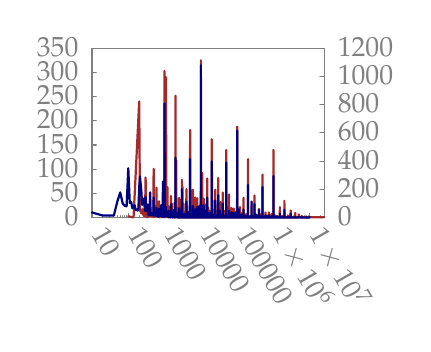
\begin{tikzpicture}[gnuplot, scale=0.3]
%% generated with GNUPLOT 5.2p2 (Lua 5.3; terminal rev. 99, script rev. 102)
%% wo 11 jul 2018 11:38:44 CEST
\path (0.000,0.000) rectangle (12.500,8.750);
\gpcolor{rgb color={0.502,0.502,0.502}}
\gpsetlinetype{gp lt border}
\gpsetdashtype{gp dt solid}
\gpsetlinewidth{1.00}
\draw[gp path] (1.012,1.264)--(1.192,1.264);
\node[gp node right] at (0.828,1.264) {$0$};
\draw[gp path] (1.012,2.289)--(1.192,2.289);
\node[gp node right] at (0.828,2.289) {$50$};
\draw[gp path] (1.012,3.315)--(1.192,3.315);
\node[gp node right] at (0.828,3.315) {$100$};
\draw[gp path] (1.012,4.340)--(1.192,4.340);
\node[gp node right] at (0.828,4.340) {$150$};
\draw[gp path] (1.012,5.365)--(1.192,5.365);
\node[gp node right] at (0.828,5.365) {$200$};
\draw[gp path] (1.012,6.390)--(1.192,6.390);
\node[gp node right] at (0.828,6.390) {$250$};
\draw[gp path] (1.012,7.416)--(1.192,7.416);
\node[gp node right] at (0.828,7.416) {$300$};
\draw[gp path] (1.012,8.441)--(1.192,8.441);
\node[gp node right] at (0.828,8.441) {$350$};
\draw[gp path] (1.012,1.264)--(1.012,1.444);
\node[gp node left,rotate=-60] at (1.012,1.080) {$10$};
\draw[gp path] (1.475,1.264)--(1.475,1.354);
\draw[gp path] (1.745,1.264)--(1.745,1.354);
\draw[gp path] (1.937,1.264)--(1.937,1.354);
\draw[gp path] (2.086,1.264)--(2.086,1.354);
\draw[gp path] (2.208,1.264)--(2.208,1.354);
\draw[gp path] (2.311,1.264)--(2.311,1.354);
\draw[gp path] (2.400,1.264)--(2.400,1.354);
\draw[gp path] (2.478,1.264)--(2.478,1.354);
\draw[gp path] (2.549,1.264)--(2.549,1.444);
\node[gp node left,rotate=-60] at (2.549,1.080) {$100$};
\draw[gp path] (3.011,1.264)--(3.011,1.354);
\draw[gp path] (3.282,1.264)--(3.282,1.354);
\draw[gp path] (3.474,1.264)--(3.474,1.354);
\draw[gp path] (3.623,1.264)--(3.623,1.354);
\draw[gp path] (3.744,1.264)--(3.744,1.354);
\draw[gp path] (3.847,1.264)--(3.847,1.354);
\draw[gp path] (3.936,1.264)--(3.936,1.354);
\draw[gp path] (4.015,1.264)--(4.015,1.354);
\draw[gp path] (4.085,1.264)--(4.085,1.444);
\node[gp node left,rotate=-60] at (4.085,1.080) {$1000$};
\draw[gp path] (4.548,1.264)--(4.548,1.354);
\draw[gp path] (4.818,1.264)--(4.818,1.354);
\draw[gp path] (5.010,1.264)--(5.010,1.354);
\draw[gp path] (5.159,1.264)--(5.159,1.354);
\draw[gp path] (5.281,1.264)--(5.281,1.354);
\draw[gp path] (5.384,1.264)--(5.384,1.354);
\draw[gp path] (5.473,1.264)--(5.473,1.354);
\draw[gp path] (5.551,1.264)--(5.551,1.354);
\draw[gp path] (5.622,1.264)--(5.622,1.444);
\node[gp node left,rotate=-60] at (5.622,1.080) {$10000$};
\draw[gp path] (6.084,1.264)--(6.084,1.354);
\draw[gp path] (6.355,1.264)--(6.355,1.354);
\draw[gp path] (6.547,1.264)--(6.547,1.354);
\draw[gp path] (6.696,1.264)--(6.696,1.354);
\draw[gp path] (6.817,1.264)--(6.817,1.354);
\draw[gp path] (6.920,1.264)--(6.920,1.354);
\draw[gp path] (7.009,1.264)--(7.009,1.354);
\draw[gp path] (7.088,1.264)--(7.088,1.354);
\draw[gp path] (7.158,1.264)--(7.158,1.444);
\node[gp node left,rotate=-60] at (7.158,1.080) {$100000$};
\draw[gp path] (7.621,1.264)--(7.621,1.354);
\draw[gp path] (7.891,1.264)--(7.891,1.354);
\draw[gp path] (8.083,1.264)--(8.083,1.354);
\draw[gp path] (8.232,1.264)--(8.232,1.354);
\draw[gp path] (8.354,1.264)--(8.354,1.354);
\draw[gp path] (8.457,1.264)--(8.457,1.354);
\draw[gp path] (8.546,1.264)--(8.546,1.354);
\draw[gp path] (8.625,1.264)--(8.625,1.354);
\draw[gp path] (8.695,1.264)--(8.695,1.444);
\node[gp node left,rotate=-60] at (8.695,1.080) {$1\times10^{6}$};
\draw[gp path] (9.157,1.264)--(9.157,1.354);
\draw[gp path] (9.428,1.264)--(9.428,1.354);
\draw[gp path] (9.620,1.264)--(9.620,1.354);
\draw[gp path] (9.769,1.264)--(9.769,1.354);
\draw[gp path] (9.891,1.264)--(9.891,1.354);
\draw[gp path] (9.994,1.264)--(9.994,1.354);
\draw[gp path] (10.083,1.264)--(10.083,1.354);
\draw[gp path] (10.161,1.264)--(10.161,1.354);
\draw[gp path] (10.232,1.264)--(10.232,1.444);
\node[gp node left,rotate=-60] at (10.232,1.080) {$1\times10^{7}$};
\draw[gp path] (10.694,1.264)--(10.694,1.354);
\draw[gp path] (10.843,1.264)--(10.663,1.264);
\node[gp node left] at (11.027,1.264) {$0$};
\draw[gp path] (10.843,2.460)--(10.663,2.460);
\node[gp node left] at (11.027,2.460) {$200$};
\draw[gp path] (10.843,3.656)--(10.663,3.656);
\node[gp node left] at (11.027,3.656) {$400$};
\draw[gp path] (10.843,4.853)--(10.663,4.853);
\node[gp node left] at (11.027,4.853) {$600$};
\draw[gp path] (10.843,6.049)--(10.663,6.049);
\node[gp node left] at (11.027,6.049) {$800$};
\draw[gp path] (10.843,7.245)--(10.663,7.245);
\node[gp node left] at (11.027,7.245) {$1000$};
\draw[gp path] (10.843,8.441)--(10.663,8.441);
\node[gp node left] at (11.027,8.441) {$1200$};
\draw[gp path] (1.012,8.441)--(1.012,1.264)--(10.843,1.264)--(10.843,8.441)--cycle;
\gpcolor{rgb color={0.647,0.165,0.165}}
\gpsetlinewidth{2.00}
\draw[gp path] (2.549,1.326)--(2.724,1.285)--(2.773,1.285)--(3.011,6.185)--(3.044,1.572)%
  --(3.075,1.510)--(3.104,1.449)--(3.133,1.490)--(3.160,1.633)--(3.186,1.387)--(3.211,1.346)%
  --(3.236,1.326)--(3.259,1.367)--(3.282,2.966)--(3.304,1.408)--(3.325,1.346)--(3.345,1.285)%
  --(3.365,1.367)--(3.385,1.674)--(3.403,1.305)--(3.422,1.326)--(3.439,1.346)--(3.457,1.387)%
  --(3.474,2.043)--(3.490,1.408)--(3.506,1.428)--(3.522,1.326)--(3.537,1.326)--(3.552,1.326)%
  --(3.581,1.305)--(3.595,1.346)--(3.609,1.326)--(3.623,3.335)--(3.636,1.346)--(3.649,1.326)%
  --(3.662,1.305)--(3.674,1.326)--(3.686,1.449)--(3.698,1.326)--(3.710,1.387)--(3.722,1.387)%
  --(3.733,1.346)--(3.744,2.535)--(3.755,1.326)--(3.766,1.408)--(3.777,1.305)--(3.787,1.408)%
  --(3.808,1.387)--(3.818,1.305)--(3.828,1.367)--(3.838,1.346)--(3.847,1.961)--(3.857,1.285)%
  --(3.866,1.285)--(3.875,1.346)--(3.884,1.305)--(3.893,1.387)--(3.902,1.305)--(3.911,1.346)%
  --(3.919,1.326)--(3.928,1.285)--(3.936,1.592)--(3.945,1.326)--(3.953,1.305)--(3.961,1.305)%
  --(3.969,1.326)--(3.977,1.305)--(3.985,1.326)--(3.992,1.305)--(4.000,1.305)--(4.007,1.305)%
  --(4.015,1.531)--(4.022,1.285)--(4.030,1.346)--(4.037,1.367)--(4.044,1.305)--(4.051,1.326)%
  --(4.058,1.305)--(4.065,1.305)--(4.072,1.326)--(4.078,1.305)--(4.085,7.477)--(4.092,1.408)%
  --(4.098,1.367)--(4.105,1.305)--(4.111,1.305)--(4.118,1.428)--(4.124,1.305)--(4.130,1.305)%
  --(4.137,1.285)--(4.143,1.367)--(4.149,7.211)--(4.155,1.531)--(4.161,1.346)--(4.167,1.469)%
  --(4.173,1.408)--(4.178,1.326)--(4.184,1.305)--(4.190,1.305)--(4.196,1.428)--(4.201,1.346)%
  --(4.207,2.556)--(4.212,1.346)--(4.218,1.285)--(4.223,1.305)--(4.229,1.305)--(4.234,1.305)%
  --(4.239,1.408)--(4.245,1.326)--(4.250,1.326)--(4.255,1.387)--(4.260,1.756)--(4.265,1.367)%
  --(4.270,1.346)--(4.275,1.428)--(4.280,1.387)--(4.285,1.346)--(4.290,1.305)--(4.295,1.305)%
  --(4.300,1.326)--(4.305,1.305)--(4.310,1.674)--(4.314,1.285)--(4.319,1.346)--(4.324,1.285)%
  --(4.329,1.346)--(4.333,1.305)--(4.338,1.305)--(4.342,1.285)--(4.347,1.326)--(4.356,2.187)%
  --(4.360,1.326)--(4.365,1.367)--(4.369,1.285)--(4.373,1.285)--(4.378,1.367)--(4.382,1.285)%
  --(4.386,1.346)--(4.390,1.305)--(4.395,1.305)--(4.399,1.859)--(4.403,1.305)--(4.407,1.285)%
  --(4.411,1.387)--(4.415,1.285)--(4.419,1.285)--(4.423,1.326)--(4.431,1.305)--(4.439,1.490)%
  --(4.443,1.305)--(4.447,1.367)--(4.451,1.285)--(4.459,1.305)--(4.462,1.305)--(4.466,1.285)%
  --(4.470,1.285)--(4.474,1.285)--(4.477,1.551)--(4.481,1.326)--(4.488,1.326)--(4.499,1.285)%
  --(4.503,1.305)--(4.506,1.305)--(4.510,1.285)--(4.514,1.408)--(4.517,1.305)--(4.520,1.285)%
  --(4.524,1.285)--(4.527,1.305)--(4.531,1.285)--(4.534,1.285)--(4.538,1.305)--(4.541,1.346)%
  --(4.548,6.431)--(4.551,1.305)--(4.554,1.285)--(4.558,1.326)--(4.561,1.285)--(4.564,1.305)%
  --(4.567,1.305)--(4.571,1.367)--(4.577,1.326)--(4.580,3.684)--(4.583,1.305)--(4.587,1.367)%
  --(4.590,1.285)--(4.593,1.346)--(4.596,1.408)--(4.599,1.285)--(4.605,1.326)--(4.608,1.346)%
  --(4.611,1.695)--(4.614,1.346)--(4.617,1.367)--(4.620,1.285)--(4.623,1.346)--(4.626,1.305)%
  --(4.632,1.285)--(4.635,1.305)--(4.638,1.326)--(4.641,1.531)--(4.644,1.346)--(4.647,1.387)%
  --(4.653,1.326)--(4.655,1.326)--(4.658,1.305)--(4.661,1.326)--(4.664,1.285)--(4.667,1.305)%
  --(4.669,1.469)--(4.672,1.285)--(4.675,1.285)--(4.678,1.346)--(4.680,1.285)--(4.683,1.346)%
  --(4.686,1.285)--(4.689,1.305)--(4.691,1.305)--(4.694,1.326)--(4.697,2.105)--(4.699,1.326)%
  --(4.702,1.285)--(4.705,1.285)--(4.707,1.285)--(4.710,1.285)--(4.712,1.387)--(4.715,1.326)%
  --(4.718,1.326)--(4.720,1.285)--(4.723,2.043)--(4.725,1.367)--(4.728,1.285)--(4.730,1.326)%
  --(4.733,1.285)--(4.736,1.408)--(4.738,1.326)--(4.741,1.346)--(4.743,1.326)--(4.748,1.326)%
  --(4.753,1.305)--(4.755,1.285)--(4.758,1.285)--(4.760,1.326)--(4.763,1.326)--(4.765,1.326)%
  --(4.767,1.285)--(4.772,1.387)--(4.775,1.326)--(4.777,1.285)--(4.779,1.285)--(4.782,1.305)%
  --(4.786,1.305)--(4.789,1.305)--(4.793,1.326)--(4.796,1.285)--(4.800,1.305)--(4.803,1.305)%
  --(4.805,1.305)--(4.807,1.285)--(4.812,1.285)--(4.814,1.305)--(4.816,1.285)--(4.818,2.863)%
  --(4.821,1.285)--(4.825,1.305)--(4.829,1.285)--(4.838,1.285)--(4.840,2.576)--(4.842,1.346)%
  --(4.844,1.305)--(4.847,1.285)--(4.849,1.285)--(4.851,1.285)--(4.853,1.285)--(4.855,1.285)%
  --(4.857,1.346)--(4.859,1.285)--(4.861,1.613)--(4.863,1.305)--(4.866,1.326)--(4.868,1.326)%
  --(4.870,1.285)--(4.872,1.326)--(4.874,1.326)--(4.878,1.285)--(4.880,1.305)--(4.882,1.449)%
  --(4.884,1.285)--(4.886,1.859)--(4.888,1.428)--(4.890,1.326)--(4.894,1.305)--(4.896,1.326)%
  --(4.900,1.305)--(4.902,1.326)--(4.904,1.285)--(4.906,1.305)--(4.908,1.367)--(4.912,1.285)%
  --(4.914,1.285)--(4.917,1.305)--(4.919,1.305)--(4.921,1.531)--(4.925,1.305)--(4.927,1.285)%
  --(4.929,1.326)--(4.933,1.305)--(4.936,1.285)--(4.938,1.305)--(4.940,1.408)--(4.942,1.305)%
  --(4.944,1.305)--(4.946,1.305)--(4.947,1.367)--(4.949,1.326)--(4.951,1.326)--(4.953,1.346)%
  --(4.955,1.285)--(4.956,1.285)--(4.958,1.387)--(4.960,1.346)--(4.964,1.285)--(4.965,1.305)%
  --(4.969,1.305)--(4.976,1.367)--(4.978,1.285)--(4.980,1.285)--(4.981,1.285)--(4.985,1.326)%
  --(4.987,1.326)--(4.988,1.326)--(4.993,1.346)--(4.995,1.285)--(4.997,1.285)--(4.999,1.285)%
  --(5.002,1.305)--(5.010,2.474)--(5.012,1.305)--(5.014,1.305)--(5.017,1.305)--(5.019,1.305)%
  --(5.022,1.305)--(5.025,1.285)--(5.027,1.736)--(5.028,1.326)--(5.030,1.285)--(5.032,1.326)%
  --(5.033,1.285)--(5.035,1.326)--(5.038,1.285)--(5.041,1.285)--(5.043,1.408)--(5.044,1.285)%
  --(5.048,1.285)--(5.049,1.285)--(5.051,1.285)--(5.054,1.285)--(5.057,1.285)--(5.059,1.408)%
  --(5.060,1.305)--(5.066,1.285)--(5.068,1.305)--(5.069,1.305)--(5.071,1.305)--(5.074,1.367)%
  --(5.075,1.285)--(5.080,1.326)--(5.081,1.285)--(5.083,1.326)--(5.084,1.285)--(5.086,1.305)%
  --(5.087,1.285)--(5.089,1.510)--(5.090,1.285)--(5.092,1.285)--(5.093,1.285)--(5.095,1.387)%
  --(5.096,1.346)--(5.098,1.326)--(5.099,1.285)--(5.102,1.305)--(5.104,1.408)--(5.109,1.285)%
  --(5.111,1.285)--(5.112,1.326)--(5.114,1.285)--(5.115,1.326)--(5.119,1.285)--(5.121,1.305)%
  --(5.122,1.285)--(5.124,1.305)--(5.125,1.305)--(5.128,1.326)--(5.132,1.408)--(5.133,1.285)%
  --(5.135,1.305)--(5.139,1.305)--(5.140,1.285)--(5.143,1.305)--(5.146,1.326)--(5.147,1.285)%
  --(5.148,1.305)--(5.157,1.285)--(5.159,4.401)--(5.161,1.305)--(5.162,1.346)--(5.165,1.285)%
  --(5.166,1.326)--(5.167,1.285)--(5.172,4.976)--(5.174,1.305)--(5.179,1.285)--(5.182,1.326)%
  --(5.183,1.285)--(5.184,1.305)--(5.185,1.531)--(5.187,1.285)--(5.188,1.346)--(5.190,1.285)%
  --(5.192,1.326)--(5.193,1.305)--(5.194,1.305)--(5.196,1.305)--(5.198,1.387)--(5.199,1.285)%
  --(5.201,1.326)--(5.203,1.285)--(5.204,1.305)--(5.206,1.285)--(5.208,1.326)--(5.209,1.305)%
  --(5.211,1.285)--(5.212,1.305)--(5.213,1.285)--(5.214,1.285)--(5.215,1.285)--(5.217,1.305)%
  --(5.220,1.285)--(5.222,1.285)--(5.223,1.387)--(5.224,1.326)--(5.225,1.285)--(5.226,1.285)%
  --(5.228,1.326)--(5.230,1.305)--(5.231,1.305)--(5.234,1.305)--(5.235,1.346)--(5.236,1.285)%
  --(5.237,1.346)--(5.240,1.305)--(5.241,1.326)--(5.244,1.305)--(5.245,1.326)--(5.247,1.285)%
  --(5.249,1.305)--(5.251,1.285)--(5.252,1.305)--(5.254,1.285)--(5.255,1.305)--(5.257,1.326)%
  --(5.258,1.305)--(5.259,1.285)--(5.262,1.285)--(5.264,1.326)--(5.267,1.305)--(5.270,1.285)%
  --(5.278,1.285)--(5.280,1.305)--(5.281,2.453)--(5.288,1.326)--(5.289,1.305)--(5.291,1.305)%
  --(5.292,2.371)--(5.293,1.346)--(5.295,1.285)--(5.298,1.285)--(5.300,1.285)--(5.302,1.285)%
  --(5.303,1.387)--(5.307,1.285)--(5.308,1.305)--(5.309,1.285)--(5.311,1.285)--(5.312,1.285)%
  --(5.313,1.305)--(5.314,1.285)--(5.316,1.285)--(5.317,1.285)--(5.318,1.285)--(5.319,1.285)%
  --(5.320,1.285)--(5.321,1.285)--(5.323,1.285)--(5.324,1.285)--(5.325,1.305)--(5.326,1.285)%
  --(5.327,1.285)--(5.328,1.305)--(5.329,1.285)--(5.330,1.285)--(5.331,1.285)--(5.334,1.408)%
  --(5.335,1.285)--(5.336,1.285)--(5.337,1.285)--(5.338,1.305)--(5.341,1.305)--(5.343,1.326)%
  --(5.344,1.408)--(5.348,1.305)--(5.349,1.367)--(5.350,1.285)--(5.351,1.326)--(5.352,1.346)%
  --(5.353,1.305)--(5.354,1.285)--(5.355,1.305)--(5.356,1.285)--(5.357,1.285)--(5.360,1.346)%
  --(5.361,1.285)--(5.362,1.326)--(5.363,1.285)--(5.364,1.285)--(5.365,1.305)--(5.366,1.285)%
  --(5.367,1.305)--(5.368,1.285)--(5.372,1.305)--(5.374,1.346)--(5.376,1.305)--(5.378,1.285)%
  --(5.379,1.305)--(5.382,1.285)--(5.384,2.125)--(5.386,1.285)--(5.389,1.285)--(5.392,1.305)%
  --(5.393,1.797)--(5.394,1.285)--(5.395,1.285)--(5.396,1.305)--(5.398,1.285)--(5.400,1.305)%
  --(5.402,1.285)--(5.403,1.387)--(5.403,1.305)--(5.406,1.285)--(5.407,1.285)--(5.410,1.285)%
  --(5.412,1.285)--(5.413,1.285)--(5.414,1.285)--(5.414,1.305)--(5.416,1.285)--(5.417,1.305)%
  --(5.421,1.305)--(5.422,1.326)--(5.423,1.285)--(5.424,1.305)--(5.427,1.285)--(5.430,1.408)%
  --(5.432,1.326)--(5.432,1.285)--(5.436,1.346)--(5.438,1.285)--(5.439,1.326)--(5.440,1.285)%
  --(5.440,1.326)--(5.442,1.285)--(5.444,1.285)--(5.445,1.285)--(5.446,1.285)--(5.447,1.305)%
  --(5.450,1.285)--(5.452,1.305)--(5.455,1.285)--(5.456,1.305)--(5.462,1.285)--(5.464,1.285)%
  --(5.465,1.285)--(5.467,1.285)--(5.469,1.285)--(5.472,1.285)--(5.473,2.084)--(5.475,1.285)%
  --(5.476,1.285)--(5.477,1.285)--(5.479,1.285)--(5.481,1.654)--(5.482,1.305)--(5.483,1.285)%
  --(5.485,1.285)--(5.486,1.285)--(5.488,1.285)--(5.489,1.305)--(5.491,1.285)--(5.493,1.285)%
  --(5.495,1.285)--(5.497,1.285)--(5.497,1.305)--(5.504,1.305)--(5.505,1.285)--(5.508,1.285)%
  --(5.509,1.285)--(5.512,1.285)--(5.513,1.326)--(5.514,1.285)--(5.516,1.285)--(5.520,1.285)%
  --(5.521,1.408)--(5.522,1.326)--(5.523,1.305)--(5.523,1.326)--(5.527,1.285)--(5.528,1.305)%
  --(5.529,1.367)--(5.530,1.305)--(5.532,1.285)--(5.533,1.285)--(5.536,1.305)--(5.537,1.285)%
  --(5.538,1.285)--(5.539,1.305)--(5.540,1.285)--(5.542,1.285)--(5.548,1.285)--(5.549,1.285)%
  --(5.550,1.285)--(5.551,1.305)--(5.551,1.695)--(5.552,1.285)--(5.553,1.285)--(5.554,1.285)%
  --(5.557,1.285)--(5.559,1.715)--(5.560,1.285)--(5.562,1.285)--(5.566,1.285)--(5.569,1.305)%
  --(5.570,1.285)--(5.573,1.285)--(5.575,1.285)--(5.577,1.305)--(5.580,1.285)--(5.583,1.285)%
  --(5.588,1.305)--(5.591,1.285)--(5.593,1.285)--(5.594,1.285)--(5.595,1.326)--(5.597,1.285)%
  --(5.598,1.285)--(5.599,1.285)--(5.601,1.346)--(5.602,1.285)--(5.603,1.285)--(5.604,1.285)%
  --(5.606,1.285)--(5.608,1.305)--(5.609,1.305)--(5.611,1.285)--(5.612,1.285)--(5.616,1.285)%
  --(5.618,1.285)--(5.619,1.285)--(5.620,1.305)--(5.621,1.326)--(5.622,7.928)--(5.622,1.346)%
  --(5.624,1.305)--(5.625,1.285)--(5.626,1.305)--(5.627,1.285)--(5.628,7.190)--(5.629,1.326)%
  --(5.631,1.285)--(5.632,1.367)--(5.634,1.285)--(5.635,1.715)--(5.636,1.305)--(5.636,1.346)%
  --(5.638,1.285)--(5.638,1.326)--(5.640,1.305)--(5.641,1.285)--(5.641,1.449)--(5.642,1.285)%
  --(5.643,1.285)--(5.645,1.285)--(5.646,1.285)--(5.647,1.285)--(5.648,1.449)--(5.649,1.305)%
  --(5.650,1.285)--(5.651,1.285)--(5.653,1.285)--(5.654,1.633)--(5.655,1.285)--(5.656,1.285)%
  --(5.657,1.285)--(5.657,1.305)--(5.658,1.285)--(5.660,1.285)--(5.661,1.285)--(5.661,1.305)%
  --(5.662,1.305)--(5.663,1.285)--(5.665,1.285)--(5.667,1.285)--(5.668,1.285)--(5.669,1.305)%
  --(5.670,1.285)--(5.672,1.285)--(5.673,1.367)--(5.675,1.285)--(5.676,1.285)--(5.677,1.305)%
  --(5.678,1.305)--(5.679,1.285)--(5.679,1.326)--(5.680,1.305)--(5.682,1.285)--(5.683,1.285)%
  --(5.684,1.285)--(5.685,1.285)--(5.685,3.151)--(5.687,1.285)--(5.688,1.285)--(5.691,1.859)%
  --(5.692,1.367)--(5.693,1.326)--(5.693,1.285)--(5.694,1.305)--(5.694,1.285)--(5.695,1.285)%
  --(5.696,1.285)--(5.697,1.285)--(5.697,1.387)--(5.698,1.285)--(5.699,1.305)--(5.699,1.285)%
  --(5.700,1.305)--(5.700,1.285)--(5.702,1.285)--(5.702,1.305)--(5.703,1.326)--(5.704,1.285)%
  --(5.705,1.285)--(5.706,1.285)--(5.707,1.285)--(5.709,1.285)--(5.710,1.305)--(5.712,1.326)%
  --(5.713,1.285)--(5.714,1.285)--(5.715,1.367)--(5.716,1.285)--(5.719,1.285)--(5.720,1.285)%
  --(5.721,1.346)--(5.722,1.305)--(5.723,1.285)--(5.724,1.285)--(5.725,1.285)--(5.726,1.285)%
  --(5.727,1.326)--(5.728,1.285)--(5.729,1.285)--(5.731,1.285)--(5.732,1.305)--(5.735,1.285)%
  --(5.736,1.285)--(5.737,1.305)--(5.740,1.285)--(5.742,1.305)--(5.743,2.064)--(5.744,1.285)%
  --(5.745,1.285)--(5.746,1.305)--(5.747,1.285)--(5.749,1.797)--(5.750,1.285)--(5.750,1.305)%
  --(5.751,1.285)--(5.752,1.285)--(5.754,1.326)--(5.757,1.285)--(5.758,1.305)--(5.759,1.285)%
  --(5.760,1.285)--(5.761,1.326)--(5.762,1.285)--(5.763,1.285)--(5.765,1.285)--(5.766,1.285)%
  --(5.769,1.285)--(5.770,1.285)--(5.771,1.367)--(5.773,1.305)--(5.773,1.285)--(5.774,1.285)%
  --(5.775,1.285)--(5.776,1.408)--(5.780,1.285)--(5.781,1.326)--(5.783,1.285)--(5.784,1.285)%
  --(5.785,1.305)--(5.787,1.285)--(5.790,1.285)--(5.791,1.285)--(5.792,1.510)--(5.792,1.285)%
  --(5.796,1.305)--(5.797,1.838)--(5.798,1.285)--(5.800,1.285)--(5.802,1.469)--(5.802,1.285)%
  --(5.803,1.285)--(5.804,1.285)--(5.806,1.285)--(5.807,1.346)--(5.809,1.285)--(5.810,1.285)%
  --(5.812,1.285)--(5.814,1.285)--(5.815,1.305)--(5.816,1.326)--(5.816,1.285)--(5.817,1.285)%
  --(5.822,1.305)--(5.824,1.305)--(5.827,1.285)--(5.828,1.285)--(5.832,1.346)--(5.832,1.285)%
  --(5.836,1.285)--(5.837,1.285)--(5.839,1.285)--(5.846,1.756)--(5.849,1.285)--(5.851,1.654)%
  --(5.852,1.285)--(5.852,1.326)--(5.853,1.285)--(5.854,1.285)--(5.855,1.326)--(5.856,1.326)%
  --(5.857,1.285)--(5.858,1.285)--(5.859,1.285)--(5.860,1.305)--(5.861,1.285)--(5.865,1.346)%
  --(5.866,1.285)--(5.867,1.285)--(5.870,1.305)--(5.872,1.305)--(5.874,1.285)--(5.875,1.305)%
  --(5.877,1.285)--(5.878,1.285)--(5.879,1.285)--(5.882,1.285)--(5.884,1.305)--(5.887,1.285)%
  --(5.888,1.305)--(5.892,1.285)--(5.892,2.925)--(5.893,1.305)--(5.893,1.285)--(5.896,1.285)%
  --(5.897,2.351)--(5.897,1.285)--(5.898,1.305)--(5.898,1.285)--(5.899,1.285)--(5.900,1.305)%
  --(5.901,1.408)--(5.902,1.285)--(5.903,1.326)--(5.903,1.285)--(5.904,1.285)--(5.906,1.285)%
  --(5.911,1.285)--(5.912,1.326)--(5.913,1.285)--(5.914,1.408)--(5.915,1.285)--(5.916,1.305)%
  --(5.916,1.285)--(5.917,1.305)--(5.918,1.285)--(5.919,1.285)--(5.921,1.305)--(5.922,1.285)%
  --(5.922,1.305)--(5.923,1.305)--(5.923,1.285)--(5.924,1.285)--(5.924,1.305)--(5.925,1.285)%
  --(5.928,1.285)--(5.930,1.285)--(5.931,1.285)--(5.933,1.285)--(5.935,1.695)--(5.936,1.305)%
  --(5.937,1.285)--(5.940,1.510)--(5.940,1.285)--(5.942,1.285)--(5.944,1.326)--(5.945,1.285)%
  --(5.946,1.285)--(5.947,1.285)--(5.949,1.285)--(5.950,1.305)--(5.952,1.285)--(5.954,1.285)%
  --(5.955,1.285)--(5.956,1.367)--(5.958,1.285)--(5.961,1.285)--(5.963,1.285)--(5.964,1.305)%
  --(5.964,1.285)--(5.968,1.285)--(5.969,1.285)--(5.970,1.285)--(5.971,1.285)--(5.973,1.285)%
  --(5.976,1.572)--(5.976,1.305)--(5.979,1.285)--(5.980,1.449)--(5.983,1.285)--(5.984,1.285)%
  --(5.986,1.305)--(5.989,1.285)--(5.991,1.285)--(5.993,1.285)--(5.994,1.285)--(5.995,1.285)%
  --(5.996,1.285)--(5.997,1.285)--(5.999,1.285)--(6.001,1.285)--(6.003,1.305)--(6.005,1.285)%
  --(6.006,1.285)--(6.007,1.285)--(6.011,1.285)--(6.013,1.285)--(6.014,1.408)--(6.015,1.285)%
  --(6.016,1.305)--(6.018,1.490)--(6.019,1.285)--(6.020,1.285)--(6.021,1.305)--(6.023,1.285)%
  --(6.024,1.285)--(6.025,1.285)--(6.025,1.305)--(6.026,1.285)--(6.028,1.285)--(6.029,1.285)%
  --(6.030,1.285)--(6.031,1.285)--(6.032,1.285)--(6.032,1.326)--(6.033,1.285)--(6.036,1.285)%
  --(6.040,1.285)--(6.041,1.285)--(6.047,1.285)--(6.049,1.285)--(6.050,1.469)--(6.053,1.285)%
  --(6.054,1.531)--(6.054,1.285)--(6.056,1.285)--(6.057,1.285)--(6.060,1.285)--(6.063,1.285)%
  --(6.069,1.285)--(6.073,1.285)--(6.078,1.305)--(6.079,1.285)--(6.081,1.285)--(6.082,1.285)%
  --(6.084,1.285)--(6.084,4.586)--(6.085,1.305)--(6.086,1.285)--(6.087,1.285)--(6.088,3.930)%
  --(6.089,1.285)--(6.089,1.305)--(6.090,1.326)--(6.090,1.305)--(6.091,1.305)--(6.091,1.510)%
  --(6.091,1.285)--(6.092,1.285)--(6.093,1.305)--(6.094,1.326)--(6.094,1.285)--(6.094,1.346)%
  --(6.095,1.285)--(6.096,1.305)--(6.096,1.285)--(6.097,1.305)--(6.097,1.285)--(6.098,1.285)%
  --(6.099,1.305)--(6.100,1.285)--(6.101,1.285)--(6.102,1.285)--(6.103,1.285)--(6.104,1.285)%
  --(6.104,1.326)--(6.105,1.285)--(6.108,1.285)--(6.110,1.285)--(6.110,1.305)--(6.113,1.285)%
  --(6.114,1.305)--(6.117,1.285)--(6.117,2.002)--(6.118,1.285)--(6.119,1.285)--(6.120,1.654)%
  --(6.120,1.305)--(6.121,1.305)--(6.122,1.285)--(6.122,1.305)--(6.123,1.285)--(6.123,1.305)%
  --(6.124,1.305)--(6.124,1.285)--(6.125,1.285)--(6.126,1.326)--(6.127,1.285)--(6.128,1.285)%
  --(6.129,1.285)--(6.130,1.285)--(6.131,1.285)--(6.133,1.387)--(6.134,1.285)--(6.135,1.285)%
  --(6.136,1.285)--(6.141,1.285)--(6.147,1.285)--(6.148,1.531)--(6.148,1.285)--(6.149,1.285)%
  --(6.150,1.285)--(6.151,1.551)--(6.152,1.305)--(6.153,1.326)--(6.153,1.305)--(6.153,1.285)%
  --(6.154,1.285)--(6.155,1.285)--(6.156,1.285)--(6.158,1.285)--(6.161,1.285)--(6.163,1.428)%
  --(6.164,1.285)--(6.165,1.285)--(6.166,1.285)--(6.168,1.326)--(6.169,1.285)--(6.171,1.285)%
  --(6.172,1.285)--(6.175,1.285)--(6.176,1.285)--(6.177,1.285)--(6.178,1.592)--(6.178,1.285)%
  --(6.180,1.285)--(6.180,1.531)--(6.181,1.285)--(6.182,1.285)--(6.183,1.305)--(6.184,1.285)%
  --(6.186,1.285)--(6.187,1.285)--(6.189,1.305)--(6.190,1.285)--(6.192,1.285)--(6.193,1.305)%
  --(6.194,1.285)--(6.195,1.285)--(6.196,1.285)--(6.198,1.305)--(6.199,1.346)--(6.200,1.305)%
  --(6.201,1.285)--(6.202,1.285)--(6.203,1.285)--(6.204,1.305)--(6.206,1.285)--(6.206,1.510)%
  --(6.209,1.305)--(6.212,1.305)--(6.214,1.305)--(6.215,1.285)--(6.219,1.285)--(6.220,1.285)%
  --(6.221,1.285)--(6.224,1.305)--(6.225,1.285)--(6.226,1.285)--(6.227,1.285)--(6.228,1.326)%
  --(6.231,1.285)--(6.232,1.285)--(6.233,1.285)--(6.233,2.453)--(6.236,2.310)--(6.237,1.285)%
  --(6.238,1.285)--(6.239,1.490)--(6.239,1.285)--(6.240,1.285)--(6.241,1.305)--(6.244,1.285)%
  --(6.245,1.305)--(6.246,1.285)--(6.247,1.285)--(6.249,1.305)--(6.250,1.285)--(6.251,1.326)%
  --(6.251,1.285)--(6.252,1.285)--(6.254,1.285)--(6.256,1.285)--(6.257,1.285)--(6.259,1.285)%
  --(6.259,1.408)--(6.262,1.490)--(6.265,1.285)--(6.266,1.285)--(6.267,1.305)--(6.267,1.285)%
  --(6.267,1.305)--(6.268,1.305)--(6.269,1.285)--(6.271,1.285)--(6.272,1.285)--(6.273,1.285)%
  --(6.274,1.285)--(6.276,1.285)--(6.277,1.285)--(6.278,1.285)--(6.279,1.285)--(6.282,1.305)%
  --(6.282,1.285)--(6.285,1.367)--(6.287,1.551)--(6.288,1.285)--(6.289,1.285)--(6.290,1.285)%
  --(6.293,1.285)--(6.294,1.285)--(6.294,1.326)--(6.296,1.285)--(6.297,1.285)--(6.297,1.326)%
  --(6.300,1.285)--(6.301,1.285)--(6.303,1.285)--(6.304,1.285)--(6.305,1.285)--(6.309,1.367)%
  --(6.311,1.285)--(6.311,1.408)--(6.315,1.285)--(6.317,1.285)--(6.319,1.285)--(6.321,1.285)%
  --(6.322,1.285)--(6.323,1.285)--(6.324,1.285)--(6.327,1.285)--(6.328,1.285)--(6.332,1.326)%
  --(6.333,1.285)--(6.334,1.285)--(6.335,1.305)--(6.337,1.285)--(6.341,1.285)--(6.346,1.305)%
  --(6.347,1.285)--(6.348,1.326)--(6.348,1.305)--(6.352,1.285)--(6.353,1.285)--(6.354,1.285)%
  --(6.355,2.945)--(6.355,1.285)--(6.356,1.285)--(6.357,1.285)--(6.357,2.351)--(6.358,1.305)%
  --(6.359,1.428)--(6.360,1.305)--(6.361,1.305)--(6.363,1.285)--(6.364,1.305)--(6.364,1.285)%
  --(6.366,1.346)--(6.366,1.285)--(6.369,1.285)--(6.370,1.285)--(6.371,1.285)--(6.372,1.285)%
  --(6.373,1.285)--(6.374,1.285)--(6.374,1.305)--(6.377,1.900)--(6.377,1.285)--(6.379,1.449)%
  --(6.380,1.285)--(6.381,1.305)--(6.383,1.305)--(6.385,1.305)--(6.386,1.285)--(6.387,1.285)%
  --(6.388,1.285)--(6.389,1.305)--(6.393,1.285)--(6.395,1.285)--(6.398,1.367)--(6.399,1.285)%
  --(6.400,1.326)--(6.401,1.285)--(6.402,1.285)--(6.404,1.285)--(6.404,1.305)--(6.405,1.285)%
  --(6.406,1.285)--(6.410,1.285)--(6.414,1.285)--(6.415,1.285)--(6.416,1.285)--(6.419,1.613)%
  --(6.421,1.305)--(6.421,1.285)--(6.423,1.285)--(6.425,1.305)--(6.425,1.285)--(6.427,1.305)%
  --(6.431,1.305)--(6.431,1.285)--(6.437,1.285)--(6.437,1.305)--(6.438,1.387)--(6.440,1.285)%
  --(6.440,1.326)--(6.442,1.285)--(6.443,1.285)--(6.445,1.285)--(6.447,1.285)--(6.448,1.285)%
  --(6.450,1.285)--(6.451,1.285)--(6.455,1.285)--(6.456,1.285)--(6.457,1.285)--(6.458,1.920)%
  --(6.459,1.285)--(6.460,1.531)--(6.461,1.285)--(6.462,1.326)--(6.463,1.285)--(6.464,1.305)%
  --(6.465,1.285)--(6.466,1.285)--(6.469,1.285)--(6.470,1.285)--(6.472,1.285)--(6.475,1.305)%
  --(6.475,1.285)--(6.477,1.285)--(6.478,1.326)--(6.480,1.285)--(6.484,1.285)--(6.486,1.326)%
  --(6.494,1.285)--(6.495,1.367)--(6.497,1.305)--(6.498,1.285)--(6.500,1.285)--(6.504,1.285)%
  --(6.506,1.285)--(6.509,1.285)--(6.513,1.305)--(6.514,1.285)--(6.514,1.326)--(6.516,1.285)%
  --(6.516,1.305)--(6.520,1.285)--(6.521,1.285)--(6.522,1.285)--(6.524,1.285)--(6.527,1.285)%
  --(6.528,1.285)--(6.528,1.305)--(6.532,1.305)--(6.537,1.285)--(6.538,1.285)--(6.540,1.305)%
  --(6.540,1.285)--(6.542,1.285)--(6.544,1.285)--(6.545,1.285)--(6.546,1.285)--(6.547,1.285)%
  --(6.547,2.330)--(6.547,1.285)--(6.548,1.285)--(6.549,2.187)--(6.549,1.285)--(6.550,1.305)%
  --(6.550,1.326)--(6.551,1.285)--(6.552,1.305)--(6.554,1.285)--(6.555,1.285)--(6.556,1.285)%
  --(6.558,1.285)--(6.559,1.285)--(6.560,1.285)--(6.562,1.285)--(6.563,1.469)--(6.564,1.285)%
  --(6.565,1.326)--(6.565,1.285)--(6.566,1.285)--(6.567,1.285)--(6.568,1.285)--(6.570,1.285)%
  --(6.571,1.305)--(6.572,1.285)--(6.573,1.285)--(6.575,1.285)--(6.576,1.285)--(6.577,1.285)%
  --(6.579,1.285)--(6.579,1.305)--(6.581,1.367)--(6.583,1.285)--(6.584,1.285)--(6.585,1.285)%
  --(6.587,1.285)--(6.589,1.285)--(6.590,1.285)--(6.595,1.305)--(6.597,1.326)--(6.597,1.285)%
  --(6.600,1.285)--(6.607,1.285)--(6.610,1.367)--(6.612,1.305)--(6.617,1.285)--(6.618,1.285)%
  --(6.619,1.285)--(6.621,1.285)--(6.622,1.285)--(6.623,1.285)--(6.625,1.469)--(6.627,1.551)%
  --(6.628,1.285)--(6.629,1.285)--(6.634,1.305)--(6.635,1.285)--(6.636,1.285)--(6.637,1.305)%
  --(6.640,1.285)--(6.640,1.346)--(6.643,1.285)--(6.644,1.285)--(6.646,1.285)--(6.647,1.285)%
  --(6.647,1.326)--(6.648,1.285)--(6.650,1.285)--(6.653,1.285)--(6.655,1.346)--(6.656,1.346)%
  --(6.657,1.285)--(6.658,1.285)--(6.659,1.285)--(6.660,1.285)--(6.663,1.285)--(6.664,1.285)%
  --(6.665,1.285)--(6.666,1.285)--(6.668,1.285)--(6.669,1.305)--(6.670,1.305)--(6.674,1.285)%
  --(6.677,1.285)--(6.678,1.285)--(6.679,1.305)--(6.682,1.285)--(6.684,1.346)--(6.684,1.285)%
  --(6.686,1.285)--(6.690,1.285)--(6.692,1.285)--(6.693,1.285)--(6.694,1.285)--(6.695,1.285)%
  --(6.696,3.499)--(6.696,1.346)--(6.696,1.285)--(6.697,4.135)--(6.697,1.285)--(6.698,1.285)%
  --(6.698,1.305)--(6.698,1.285)--(6.698,1.572)--(6.699,1.285)--(6.699,1.305)--(6.700,1.285)%
  --(6.700,1.490)--(6.700,1.285)--(6.701,1.305)--(6.701,1.285)--(6.702,1.285)--(6.702,1.367)%
  --(6.704,1.285)--(6.704,1.326)--(6.704,1.285)--(6.705,1.285)--(6.706,1.285)--(6.707,1.285)%
  --(6.708,1.326)--(6.708,1.285)--(6.709,1.285)--(6.709,1.715)--(6.710,1.285)--(6.710,1.346)%
  --(6.710,1.305)--(6.712,1.305)--(6.712,1.285)--(6.713,1.285)--(6.714,1.285)--(6.714,1.305)%
  --(6.714,1.285)--(6.714,1.305)--(6.714,1.285)--(6.715,1.285)--(6.716,1.285)--(6.717,1.285)%
  --(6.718,1.285)--(6.718,1.326)--(6.719,1.285)--(6.720,1.285)--(6.721,1.285)--(6.722,1.469)%
  --(6.722,1.285)--(6.723,1.449)--(6.724,1.285)--(6.725,1.285)--(6.729,1.285)--(6.732,1.285)%
  --(6.733,1.285)--(6.733,1.305)--(6.735,1.346)--(6.735,1.285)--(6.736,1.285)--(6.737,1.305)%
  --(6.738,1.285)--(6.740,1.285)--(6.741,1.285)--(6.743,1.285)--(6.744,1.285)--(6.745,1.285)%
  --(6.746,1.285)--(6.747,1.367)--(6.748,1.346)--(6.750,1.326)--(6.751,1.428)--(6.752,1.285)%
  --(6.753,1.285)--(6.755,1.285)--(6.756,1.285)--(6.757,1.285)--(6.757,1.326)--(6.758,1.285)%
  --(6.759,1.510)--(6.760,1.285)--(6.761,1.449)--(6.761,1.285)--(6.762,1.285)--(6.763,1.285)%
  --(6.765,1.285)--(6.767,1.285)--(6.771,1.285)--(6.774,1.285)--(6.777,1.285)--(6.779,1.285)%
  --(6.779,1.326)--(6.780,1.387)--(6.780,1.285)--(6.781,1.285)--(6.782,1.285)--(6.783,1.285)%
  --(6.785,1.305)--(6.786,1.285)--(6.787,1.285)--(6.788,1.285)--(6.789,1.285)--(6.790,1.285)%
  --(6.791,1.285)--(6.794,1.285)--(6.795,1.285)--(6.796,1.285)--(6.801,1.285)--(6.803,1.285)%
  --(6.804,1.285)--(6.806,1.305)--(6.807,1.285)--(6.808,1.285)--(6.809,1.285)--(6.810,1.285)%
  --(6.814,1.285)--(6.815,1.285)--(6.816,1.285)--(6.817,2.248)--(6.818,1.285)--(6.819,1.715)%
  --(6.819,1.285)--(6.820,1.305)--(6.820,1.285)--(6.821,1.285)--(6.822,1.285)--(6.823,1.285)%
  --(6.824,1.305)--(6.825,1.305)--(6.825,1.285)--(6.826,1.285)--(6.827,1.285)--(6.828,1.285)%
  --(6.828,1.387)--(6.830,1.305)--(6.831,1.285)--(6.832,1.285)--(6.833,1.305)--(6.834,1.285)%
  --(6.837,1.285)--(6.839,1.305)--(6.841,1.285)--(6.842,1.285)--(6.845,1.305)--(6.846,1.285)%
  --(6.847,1.285)--(6.849,1.285)--(6.850,1.346)--(6.850,1.285)--(6.851,1.285)--(6.851,1.305)%
  --(6.851,1.285)--(6.852,1.285)--(6.853,1.285)--(6.855,1.285)--(6.856,1.285)--(6.857,1.285)%
  --(6.861,1.305)--(6.861,1.285)--(6.862,1.285)--(6.863,1.285)--(6.867,1.285)--(6.870,1.285)%
  --(6.871,1.285)--(6.871,1.490)--(6.871,1.285)--(6.872,1.346)--(6.872,1.285)--(6.874,1.285)%
  --(6.875,1.285)--(6.878,1.285)--(6.879,1.285)--(6.880,1.285)--(6.881,1.346)--(6.882,1.285)%
  --(6.884,1.285)--(6.884,1.305)--(6.887,1.285)--(6.889,1.285)--(6.890,1.285)--(6.891,1.305)%
  --(6.892,1.305)--(6.893,1.285)--(6.898,1.285)--(6.900,1.285)--(6.901,1.367)--(6.901,1.285)%
  --(6.902,1.285)--(6.903,1.285)--(6.906,1.285)--(6.911,1.285)--(6.912,1.346)--(6.913,1.285)%
  --(6.914,1.285)--(6.915,1.285)--(6.920,1.285)--(6.920,1.674)--(6.921,1.285)--(6.921,1.449)%
  --(6.921,1.285)--(6.922,1.285)--(6.922,1.326)--(6.922,1.285)--(6.923,1.285)--(6.924,1.285)%
  --(6.926,1.285)--(6.930,1.285)--(6.931,1.285)--(6.932,1.285)--(6.933,1.285)--(6.937,1.285)%
  --(6.939,1.305)--(6.940,1.305)--(6.946,1.285)--(6.947,1.285)--(6.954,1.285)--(6.955,1.285)%
  --(6.956,1.285)--(6.957,1.285)--(6.957,1.305)--(6.958,1.285)--(6.961,1.326)--(6.961,1.285)%
  --(6.966,1.510)--(6.967,1.367)--(6.968,1.285)--(6.969,1.285)--(6.972,1.285)--(6.973,1.285)%
  --(6.975,1.305)--(6.976,1.285)--(6.977,1.285)--(6.978,1.285)--(6.980,1.285)--(6.982,1.285)%
  --(6.984,1.285)--(6.985,1.285)--(6.989,1.285)--(6.990,1.285)--(6.993,1.285)--(7.000,1.285)%
  --(7.001,1.285)--(7.002,1.285)--(7.008,1.285)--(7.009,1.285)--(7.009,1.613)--(7.010,1.285)%
  --(7.010,1.654)--(7.011,1.285)--(7.012,1.285)--(7.013,1.285)--(7.018,1.285)--(7.019,1.285)%
  --(7.020,1.285)--(7.022,1.285)--(7.023,1.285)--(7.027,1.305)--(7.028,1.285)--(7.029,1.285)%
  --(7.032,1.285)--(7.034,1.285)--(7.035,1.285)--(7.035,1.305)--(7.040,1.285)--(7.042,1.285)%
  --(7.043,1.285)--(7.050,1.346)--(7.051,1.285)--(7.052,1.285)--(7.053,1.285)--(7.058,1.305)%
  --(7.062,1.285)--(7.065,1.305)--(7.065,1.285)--(7.066,1.285)--(7.067,1.285)--(7.069,1.285)%
  --(7.073,1.305)--(7.073,1.285)--(7.074,1.285)--(7.075,1.285)--(7.077,1.285)--(7.081,1.285)%
  --(7.082,1.285)--(7.088,1.510)--(7.088,1.285)--(7.089,1.408)--(7.090,1.326)--(7.090,1.285)%
  --(7.092,1.285)--(7.094,1.285)--(7.095,1.285)--(7.096,1.285)--(7.103,1.285)--(7.105,1.305)%
  --(7.108,1.285)--(7.114,1.285)--(7.115,1.285)--(7.116,1.285)--(7.118,1.285)--(7.119,1.285)%
  --(7.120,1.285)--(7.124,1.285)--(7.125,1.305)--(7.125,1.285)--(7.126,1.285)--(7.127,1.305)%
  --(7.131,1.285)--(7.138,1.285)--(7.140,1.285)--(7.141,1.285)--(7.142,1.285)--(7.143,1.285)%
  --(7.145,1.285)--(7.145,1.326)--(7.151,1.285)--(7.152,1.285)--(7.153,1.285)--(7.155,1.285)%
  --(7.158,4.811)--(7.158,1.285)--(7.159,5.119)--(7.159,1.285)--(7.159,1.305)--(7.160,1.285)%
  --(7.160,1.961)--(7.160,1.285)--(7.160,1.367)--(7.161,1.285)--(7.161,1.428)--(7.161,1.305)%
  --(7.162,1.346)--(7.162,1.285)--(7.163,1.285)--(7.164,1.285)--(7.165,1.285)--(7.165,1.736)%
  --(7.165,1.285)--(7.166,1.285)--(7.166,1.305)--(7.167,1.285)--(7.168,1.285)--(7.169,1.285)%
  --(7.170,1.285)--(7.171,1.285)--(7.172,1.408)--(7.172,1.285)--(7.173,1.305)--(7.173,1.285)%
  --(7.174,1.285)--(7.175,1.285)--(7.176,1.285)--(7.177,1.285)--(7.178,1.285)--(7.179,1.285)%
  --(7.180,1.285)--(7.181,1.285)--(7.182,1.285)--(7.183,1.285)--(7.185,1.326)--(7.185,1.285)%
  --(7.186,1.285)--(7.188,1.285)--(7.189,1.285)--(7.190,1.285)--(7.191,1.285)--(7.191,1.408)%
  --(7.191,1.285)--(7.192,1.285)--(7.193,1.285)--(7.194,1.285)--(7.195,1.285)--(7.196,1.285)%
  --(7.197,1.285)--(7.197,1.346)--(7.198,1.326)--(7.198,1.285)--(7.199,1.285)--(7.202,1.285)%
  --(7.203,1.285)--(7.204,1.367)--(7.204,1.285)--(7.205,1.285)--(7.206,1.285)--(7.207,1.285)%
  --(7.208,1.285)--(7.210,1.305)--(7.210,1.285)--(7.211,1.285)--(7.212,1.285)--(7.214,1.285)%
  --(7.215,1.285)--(7.216,1.326)--(7.216,1.285)--(7.217,1.285)--(7.218,1.285)--(7.219,1.285)%
  --(7.221,1.285)--(7.222,1.633)--(7.222,1.285)--(7.223,1.326)--(7.223,1.285)--(7.224,1.285)%
  --(7.225,1.285)--(7.227,1.285)--(7.228,1.346)--(7.228,1.285)--(7.229,1.326)--(7.229,1.346)%
  --(7.229,1.285)--(7.230,1.305)--(7.230,1.285)--(7.231,1.285)--(7.232,1.285)--(7.233,1.285)%
  --(7.235,1.305)--(7.236,1.285)--(7.237,1.285)--(7.238,1.285)--(7.240,1.285)--(7.244,1.285)%
  --(7.245,1.285)--(7.246,1.285)--(7.249,1.285)--(7.250,1.285)--(7.252,1.326)--(7.252,1.285)%
  --(7.253,1.285)--(7.257,1.285)--(7.260,1.285)--(7.261,1.285)--(7.263,1.285)--(7.264,1.285)%
  --(7.265,1.285)--(7.267,1.285)--(7.268,1.285)--(7.270,1.285)--(7.272,1.285)--(7.274,1.285)%
  --(7.274,1.326)--(7.274,1.285)--(7.276,1.285)--(7.280,1.715)--(7.281,1.469)--(7.281,1.285)%
  --(7.281,1.305)--(7.282,1.285)--(7.284,1.285)--(7.285,1.285)--(7.286,1.408)--(7.286,1.285)%
  --(7.287,1.285)--(7.291,1.346)--(7.292,1.305)--(7.292,1.285)--(7.294,1.305)--(7.296,1.285)%
  --(7.298,1.285)--(7.300,1.285)--(7.302,1.285)--(7.304,1.285)--(7.305,1.285)--(7.306,1.285)%
  --(7.307,1.490)--(7.308,1.346)--(7.308,1.285)--(7.310,1.285)--(7.313,1.285)--(7.315,1.285)%
  --(7.316,1.285)--(7.318,1.326)--(7.320,1.285)--(7.322,1.285)--(7.324,1.285)--(7.327,1.285)%
  --(7.329,1.285)--(7.331,1.285)--(7.333,1.428)--(7.334,1.285)--(7.334,1.305)--(7.334,1.285)%
  --(7.334,1.305)--(7.335,1.285)--(7.337,1.285)--(7.339,1.285)--(7.342,1.285)--(7.344,1.326)%
  --(7.344,1.285)--(7.350,1.285)--(7.351,1.285)--(7.352,1.285)--(7.353,1.285)--(7.356,1.285)%
  --(7.358,1.285)--(7.359,1.305)--(7.361,1.285)--(7.364,1.285)--(7.366,1.285)--(7.368,1.285)%
  --(7.373,1.285)--(7.374,1.285)--(7.376,1.285)--(7.378,1.285)--(7.382,1.285)--(7.383,1.387)%
  --(7.383,1.285)--(7.384,1.305)--(7.385,1.285)--(7.387,1.285)--(7.388,1.305)--(7.388,1.285)%
  --(7.389,1.285)--(7.390,1.285)--(7.390,1.326)--(7.390,1.285)--(7.391,1.285)--(7.392,1.285)%
  --(7.394,1.285)--(7.397,1.305)--(7.398,1.285)--(7.399,1.285)--(7.402,1.285)--(7.403,1.285)%
  --(7.406,1.285)--(7.409,1.285)--(7.411,1.285)--(7.414,1.285)--(7.415,1.285)--(7.416,1.285)%
  --(7.420,1.285)--(7.422,1.285)--(7.427,1.285)--(7.429,2.105)--(7.429,2.023)--(7.430,1.285)%
  --(7.430,1.305)--(7.431,1.285)--(7.432,1.285)--(7.433,1.285)--(7.433,1.469)--(7.434,1.285)%
  --(7.438,1.285)--(7.439,1.285)--(7.443,1.285)--(7.444,1.285)--(7.445,1.285)--(7.446,1.305)%
  --(7.447,1.285)--(7.449,1.285)--(7.451,1.285)--(7.452,1.285)--(7.453,1.285)--(7.455,1.305)%
  --(7.457,1.285)--(7.459,1.285)--(7.460,1.285)--(7.461,1.285)--(7.464,1.285)--(7.467,1.285)%
  --(7.468,1.285)--(7.469,1.285)--(7.472,1.367)--(7.472,1.305)--(7.473,1.285)--(7.480,1.285)%
  --(7.481,1.305)--(7.483,1.285)--(7.484,1.285)--(7.485,1.285)--(7.487,1.285)--(7.488,1.285)%
  --(7.489,1.285)--(7.490,1.285)--(7.493,1.285)--(7.497,1.285)--(7.500,1.285)--(7.504,1.285)%
  --(7.505,1.285)--(7.509,1.285)--(7.511,1.285)--(7.512,1.285)--(7.512,1.387)--(7.513,1.285)%
  --(7.513,1.305)--(7.513,1.285)--(7.514,1.285)--(7.516,1.285)--(7.516,1.305)--(7.517,1.285)%
  --(7.518,1.285)--(7.520,1.285)--(7.521,1.285)--(7.523,1.285)--(7.524,1.285)--(7.525,1.285)%
  --(7.529,1.285)--(7.532,1.326)--(7.532,1.305)--(7.534,1.285)--(7.538,1.285)--(7.539,1.305)%
  --(7.540,1.285)--(7.547,1.285)--(7.548,1.285)--(7.550,1.285)--(7.551,1.428)--(7.551,1.326)%
  --(7.551,1.285)--(7.553,1.285)--(7.555,1.285)--(7.557,1.285)--(7.560,1.285)--(7.561,1.285)%
  --(7.562,1.285)--(7.563,1.285)--(7.565,1.285)--(7.567,1.285)--(7.568,1.285)--(7.570,1.285)%
  --(7.573,1.285)--(7.580,1.285)--(7.581,1.285)--(7.583,1.285)--(7.587,1.387)--(7.587,1.305)%
  --(7.590,1.285)--(7.593,1.285)--(7.601,1.285)--(7.604,1.305)--(7.606,1.285)--(7.615,1.285)%
  --(7.618,1.285)--(7.621,1.285)--(7.621,3.745)--(7.621,1.285)--(7.621,2.863)--(7.622,1.490)%
  --(7.622,1.285)--(7.623,1.285)--(7.623,1.326)--(7.623,1.285)--(7.624,1.346)--(7.624,1.285)%
  --(7.625,1.285)--(7.626,1.285)--(7.627,1.285)--(7.627,1.305)--(7.628,1.285)--(7.629,1.285)%
  --(7.630,1.285)--(7.631,1.285)--(7.632,1.285)--(7.634,1.285)--(7.635,1.285)--(7.636,1.305)%
  --(7.637,1.285)--(7.638,1.285)--(7.639,1.285)--(7.640,1.285)--(7.641,1.326)--(7.644,1.285)%
  --(7.645,1.285)--(7.653,1.346)--(7.654,1.346)--(7.654,1.285)--(7.655,1.285)--(7.656,1.285)%
  --(7.657,1.285)--(7.658,1.285)--(7.659,1.285)--(7.660,1.285)--(7.661,1.285)--(7.662,1.285)%
  --(7.663,1.305)--(7.664,1.285)--(7.665,1.285)--(7.666,1.285)--(7.668,1.285)--(7.669,1.305)%
  --(7.670,1.285)--(7.671,1.285)--(7.676,1.285)--(7.679,1.285)--(7.680,1.285)--(7.681,1.285)%
  --(7.682,1.285)--(7.684,1.285)--(7.685,1.285)--(7.687,1.285)--(7.691,1.305)--(7.691,1.285)%
  --(7.692,1.285)--(7.693,1.285)--(7.694,1.285)--(7.696,1.285)--(7.700,1.305)--(7.700,1.285)%
  --(7.701,1.285)--(7.702,1.285)--(7.707,1.285)--(7.714,1.285)--(7.714,1.305)--(7.717,1.285)%
  --(7.718,1.285)--(7.723,1.285)--(7.724,1.285)--(7.725,1.285)--(7.729,1.305)--(7.729,1.285)%
  --(7.730,1.285)--(7.731,1.285)--(7.734,1.285)--(7.742,1.285)--(7.743,1.285)--(7.750,1.285)%
  --(7.756,1.285)--(7.757,1.285)--(7.759,1.285)--(7.760,1.285)--(7.762,1.285)--(7.763,1.285)%
  --(7.766,1.285)--(7.768,1.285)--(7.770,1.941)--(7.770,1.838)--(7.770,1.285)--(7.770,1.305)%
  --(7.771,1.285)--(7.772,1.387)--(7.774,1.285)--(7.775,1.285)--(7.776,1.285)--(7.777,1.285)%
  --(7.780,1.285)--(7.783,1.285)--(7.785,1.285)--(7.786,1.285)--(7.788,1.285)--(7.789,1.285)%
  --(7.796,1.285)--(7.797,1.285)--(7.799,1.285)--(7.801,1.285)--(7.802,1.285)--(7.804,1.285)%
  --(7.809,1.285)--(7.811,1.285)--(7.812,1.285)--(7.813,1.285)--(7.816,1.285)--(7.817,1.285)%
  --(7.820,1.285)--(7.821,1.346)--(7.822,1.285)--(7.824,1.285)--(7.826,1.305)--(7.840,1.285)%
  --(7.845,1.326)--(7.848,1.285)--(7.859,1.285)--(7.861,1.285)--(7.863,1.285)--(7.864,1.285)%
  --(7.865,1.285)--(7.869,1.305)--(7.869,1.285)--(7.871,1.285)--(7.873,1.285)--(7.876,1.285)%
  --(7.881,1.285)--(7.887,1.285)--(7.891,2.207)--(7.892,1.674)--(7.892,1.285)--(7.892,1.346)%
  --(7.892,1.285)--(7.894,1.285)--(7.895,1.285)--(7.896,1.285)--(7.898,1.305)--(7.900,1.285)%
  --(7.902,1.285)--(7.903,1.305)--(7.903,1.285)--(7.904,1.285)--(7.913,1.326)--(7.914,1.285)%
  --(7.916,1.285)--(7.918,1.285)--(7.919,1.285)--(7.920,1.285)--(7.921,1.285)--(7.922,1.285)%
  --(7.924,1.285)--(7.927,1.285)--(7.930,1.285)--(7.932,1.285)--(7.935,1.346)--(7.936,1.285)%
  --(7.937,1.285)--(7.941,1.285)--(7.946,1.285)--(7.955,1.285)--(7.959,1.285)--(7.962,1.285)%
  --(7.964,1.285)--(7.967,1.285)--(7.969,1.285)--(7.973,1.285)--(7.977,1.285)--(7.982,1.285)%
  --(7.983,1.285)--(7.987,1.285)--(7.989,1.285)--(7.991,1.285)--(7.994,1.387)--(7.995,1.346)%
  --(7.995,1.285)--(7.996,1.305)--(7.997,1.285)--(8.000,1.285)--(8.002,1.285)--(8.004,1.285)%
  --(8.006,1.285)--(8.010,1.285)--(8.012,1.285)--(8.013,1.285)--(8.017,1.285)--(8.020,1.285)%
  --(8.021,1.285)--(8.022,1.285)--(8.024,1.285)--(8.025,1.285)--(8.032,1.285)--(8.035,1.285)%
  --(8.040,1.285)--(8.046,1.285)--(8.052,1.285)--(8.062,1.285)--(8.067,1.285)--(8.067,1.305)%
  --(8.071,1.285)--(8.075,1.285)--(8.079,1.285)--(8.083,1.285)--(8.083,1.613)--(8.083,1.285)%
  --(8.084,1.285)--(8.084,1.633)--(8.084,1.285)--(8.084,1.326)--(8.085,1.285)--(8.086,1.285)%
  --(8.087,1.305)--(8.087,1.285)--(8.089,1.285)--(8.091,1.285)--(8.092,1.285)--(8.093,1.285)%
  --(8.095,1.285)--(8.096,1.285)--(8.097,1.285)--(8.098,1.285)--(8.100,1.285)--(8.100,1.305)%
  --(8.101,1.285)--(8.102,1.285)--(8.104,1.285)--(8.106,1.285)--(8.109,1.285)--(8.110,1.285)%
  --(8.111,1.285)--(8.113,1.285)--(8.115,1.285)--(8.116,1.285)--(8.118,1.285)--(8.119,1.285)%
  --(8.121,1.285)--(8.130,1.285)--(8.131,1.285)--(8.132,1.285)--(8.133,1.285)--(8.136,1.305)%
  --(8.141,1.285)--(8.147,1.305)--(8.147,1.285)--(8.149,1.285)--(8.153,1.285)--(8.160,1.285)%
  --(8.162,1.408)--(8.162,1.285)--(8.163,1.285)--(8.164,1.285)--(8.165,1.285)--(8.170,1.285)%
  --(8.172,1.285)--(8.175,1.285)--(8.183,1.285)--(8.184,1.285)--(8.193,1.285)--(8.194,1.285)%
  --(8.200,1.285)--(8.202,1.285)--(8.204,1.285)--(8.205,1.285)--(8.209,1.285)--(8.219,1.285)%
  --(8.220,1.285)--(8.221,1.285)--(8.224,1.285)--(8.228,1.285)--(8.230,1.285)--(8.231,1.285)%
  --(8.232,1.285)--(8.232,3.089)--(8.233,2.187)--(8.233,1.305)--(8.234,1.367)--(8.234,1.285)%
  --(8.235,1.285)--(8.236,1.285)--(8.239,1.285)--(8.240,1.285)--(8.242,1.285)--(8.244,1.285)%
  --(8.246,1.326)--(8.246,1.285)--(8.247,1.285)--(8.251,1.285)--(8.252,1.285)--(8.256,1.285)%
  --(8.259,1.326)--(8.259,1.285)--(8.262,1.285)--(8.263,1.285)--(8.264,1.285)--(8.266,1.285)%
  --(8.269,1.285)--(8.273,1.305)--(8.273,1.285)--(8.274,1.285)--(8.279,1.285)--(8.280,1.285)%
  --(8.281,1.285)--(8.282,1.285)--(8.284,1.285)--(8.286,1.285)--(8.287,1.285)--(8.290,1.285)%
  --(8.291,1.285)--(8.294,1.285)--(8.295,1.285)--(8.296,1.326)--(8.296,1.305)--(8.296,1.285)%
  --(8.297,1.285)--(8.298,1.285)--(8.299,1.285)--(8.300,1.285)--(8.302,1.285)--(8.303,1.285)%
  --(8.304,1.285)--(8.306,1.285)--(8.308,1.285)--(8.309,1.285)--(8.310,1.285)--(8.312,1.285)%
  --(8.313,1.285)--(8.315,1.285)--(8.316,1.285)--(8.319,1.285)--(8.325,1.285)--(8.330,1.285)%
  --(8.331,1.285)--(8.333,1.285)--(8.345,1.285)--(8.346,1.285)--(8.347,1.285)--(8.348,1.285)%
  --(8.351,1.285)--(8.354,1.490)--(8.354,1.449)--(8.354,1.285)--(8.355,1.285)--(8.356,1.285)%
  --(8.357,1.285)--(8.358,1.285)--(8.359,1.285)--(8.360,1.285)--(8.363,1.285)--(8.369,1.285)%
  --(8.370,1.285)--(8.371,1.285)--(8.379,1.285)--(8.385,1.285)--(8.386,1.285)--(8.387,1.285)%
  --(8.393,1.285)--(8.394,1.285)--(8.395,1.285)--(8.396,1.285)--(8.397,1.285)--(8.398,1.285)%
  --(8.401,1.285)--(8.407,1.305)--(8.408,1.285)--(8.410,1.285)--(8.412,1.285)--(8.421,1.285)%
  --(8.426,1.285)--(8.448,1.285)--(8.454,1.285)--(8.455,1.285)--(8.457,1.367)--(8.457,1.326)%
  --(8.458,1.285)--(8.459,1.285)--(8.460,1.285)--(8.463,1.285)--(8.465,1.285)--(8.467,1.285)%
  --(8.471,1.285)--(8.472,1.285)--(8.480,1.285)--(8.481,1.285)--(8.484,1.285)--(8.486,1.285)%
  --(8.487,1.285)--(8.491,1.285)--(8.495,1.285)--(8.502,1.285)--(8.503,1.490)--(8.503,1.285)%
  --(8.504,1.285)--(8.506,1.285)--(8.507,1.285)--(8.509,1.285)--(8.514,1.285)--(8.524,1.285)%
  --(8.527,1.285)--(8.529,1.285)--(8.531,1.285)--(8.536,1.285)--(8.538,1.326)--(8.541,1.285)%
  --(8.544,1.285)--(8.546,1.367)--(8.546,1.305)--(8.546,1.285)--(8.547,1.285)--(8.548,1.285)%
  --(8.549,1.285)--(8.552,1.285)--(8.554,1.285)--(8.555,1.285)--(8.558,1.285)--(8.564,1.285)%
  --(8.567,1.285)--(8.574,1.285)--(8.577,1.285)--(8.582,1.285)--(8.587,1.285)--(8.589,1.285)%
  --(8.594,1.285)--(8.599,1.285)--(8.604,1.285)--(8.606,1.285)--(8.617,1.285)--(8.618,1.285)%
  --(8.625,1.285)--(8.625,1.428)--(8.625,1.285)--(8.626,1.285)--(8.628,1.285)--(8.629,1.285)%
  --(8.634,1.285)--(8.636,1.285)--(8.638,1.285)--(8.641,1.285)--(8.650,1.285)--(8.658,1.285)%
  --(8.659,1.285)--(8.663,1.285)--(8.664,1.285)--(8.678,1.285)--(8.684,1.285)--(8.689,1.285)%
  --(8.695,1.285)--(8.695,4.135)--(8.695,2.884)--(8.695,1.285)--(8.695,1.346)--(8.695,1.305)%
  --(8.695,1.285)--(8.695,1.305)--(8.695,1.285)--(8.696,1.285)--(8.696,1.305)--(8.696,1.346)%
  --(8.696,1.285)--(8.697,1.285)--(8.698,1.285)--(8.700,1.285)--(8.701,1.285)--(8.702,1.305)%
  --(8.702,1.285)--(8.704,1.285)--(8.705,1.285)--(8.706,1.285)--(8.707,1.285)--(8.708,1.285)%
  --(8.709,1.285)--(8.710,1.285)--(8.713,1.285)--(8.714,1.285)--(8.715,1.285)--(8.716,1.285)%
  --(8.717,1.285)--(8.723,1.285)--(8.724,1.285)--(8.726,1.285)--(8.728,1.285)--(8.731,1.285)%
  --(8.732,1.285)--(8.733,1.285)--(8.734,1.285)--(8.735,1.285)--(8.739,1.285)--(8.745,1.285)%
  --(8.746,1.285)--(8.749,1.285)--(8.753,1.285)--(8.754,1.285)--(8.757,1.285)--(8.758,1.285)%
  --(8.759,1.367)--(8.759,1.305)--(8.759,1.285)--(8.760,1.285)--(8.761,1.285)--(8.763,1.285)%
  --(8.765,1.305)--(8.765,1.285)--(8.769,1.285)--(8.770,1.285)--(8.774,1.285)--(8.776,1.285)%
  --(8.778,1.285)--(8.779,1.285)--(8.785,1.285)--(8.786,1.285)--(8.788,1.285)--(8.789,1.285)%
  --(8.792,1.285)--(8.793,1.285)--(8.794,1.285)--(8.809,1.285)--(8.814,1.285)--(8.816,1.285)%
  --(8.817,1.305)--(8.817,1.326)--(8.817,1.285)--(8.818,1.285)--(8.818,1.305)--(8.820,1.285)%
  --(8.822,1.285)--(8.824,1.285)--(8.827,1.285)--(8.828,1.285)--(8.831,1.285)--(8.836,1.285)%
  --(8.837,1.285)--(8.842,1.285)--(8.844,1.305)--(8.847,1.285)--(8.849,1.326)--(8.855,1.285)%
  --(8.870,1.285)--(8.870,1.326)--(8.871,1.285)--(8.872,1.285)--(8.876,1.285)--(8.885,1.285)%
  --(8.887,1.285)--(8.892,1.285)--(8.896,1.285)--(8.904,1.285)--(8.907,1.285)--(8.909,1.285)%
  --(8.915,1.285)--(8.919,1.305)--(8.920,1.285)--(8.921,1.285)--(8.922,1.285)--(8.924,1.285)%
  --(8.927,1.285)--(8.931,1.285)--(8.932,1.285)--(8.952,1.285)--(8.963,1.285)--(8.964,1.285)%
  --(8.966,1.715)--(8.966,1.387)--(8.966,1.285)--(8.967,1.285)--(8.969,1.285)--(8.975,1.285)%
  --(8.976,1.285)--(8.987,1.305)--(8.988,1.285)--(8.989,1.285)--(8.990,1.285)--(8.995,1.285)%
  --(8.997,1.285)--(9.000,1.285)--(9.004,1.285)--(9.009,1.285)--(9.009,1.346)--(9.009,1.285)%
  --(9.010,1.285)--(9.012,1.285)--(9.016,1.285)--(9.025,1.285)--(9.029,1.285)--(9.040,1.285)%
  --(9.048,1.285)--(9.049,1.285)--(9.050,1.285)--(9.051,1.285)--(9.056,1.285)--(9.061,1.285)%
  --(9.062,1.285)--(9.067,1.285)--(9.068,1.285)--(9.072,1.285)--(9.075,1.285)--(9.085,1.285)%
  --(9.087,1.346)--(9.088,1.285)--(9.090,1.285)--(9.091,1.285)--(9.097,1.285)--(9.098,1.285)%
  --(9.101,1.285)--(9.104,1.285)--(9.107,1.285)--(9.110,1.285)--(9.114,1.285)--(9.122,1.285)%
  --(9.124,1.285)--(9.130,1.285)--(9.131,1.285)--(9.140,1.285)--(9.141,1.285)--(9.147,1.285)%
  --(9.156,1.285)--(9.157,1.982)--(9.158,1.654)--(9.158,1.285)--(9.158,1.346)--(9.158,1.285)%
  --(9.158,1.305)--(9.158,1.285)--(9.159,1.285)--(9.160,1.285)--(9.164,1.285)--(9.169,1.285)%
  --(9.170,1.285)--(9.176,1.285)--(9.177,1.285)--(9.178,1.285)--(9.181,1.285)--(9.187,1.285)%
  --(9.190,1.285)--(9.190,1.305)--(9.196,1.285)--(9.202,1.285)--(9.206,1.305)--(9.206,1.285)%
  --(9.207,1.285)--(9.208,1.285)--(9.214,1.285)--(9.218,1.285)--(9.221,1.285)--(9.222,1.285)%
  --(9.228,1.285)--(9.236,1.285)--(9.239,1.285)--(9.241,1.285)--(9.244,1.285)--(9.248,1.285)%
  --(9.249,1.285)--(9.251,1.285)--(9.253,1.285)--(9.257,1.285)--(9.258,1.285)--(9.260,1.285)%
  --(9.263,1.285)--(9.267,1.285)--(9.275,1.285)--(9.279,1.285)--(9.280,1.285)--(9.281,1.285)%
  --(9.284,1.285)--(9.291,1.285)--(9.293,1.285)--(9.297,1.285)--(9.300,1.285)--(9.301,1.285)%
  --(9.302,1.285)--(9.304,1.285)--(9.306,1.367)--(9.306,1.285)--(9.307,1.285)--(9.309,1.285)%
  --(9.320,1.285)--(9.321,1.285)--(9.330,1.285)--(9.331,1.285)--(9.333,1.285)--(9.339,1.285)%
  --(9.340,1.285)--(9.343,1.285)--(9.346,1.285)--(9.349,1.285)--(9.356,1.285)--(9.358,1.285)%
  --(9.369,1.285)--(9.370,1.285)--(9.372,1.285)--(9.382,1.285)--(9.384,1.285)--(9.396,1.285)%
  --(9.398,1.285)--(9.406,1.285)--(9.409,1.285)--(9.428,1.572)--(9.428,1.469)--(9.428,1.285)%
  --(9.429,1.285)--(9.431,1.285)--(9.433,1.285)--(9.434,1.285)--(9.438,1.285)--(9.440,1.285)%
  --(9.442,1.285)--(9.443,1.285)--(9.448,1.285)--(9.449,1.285)--(9.450,1.285)--(9.452,1.285)%
  --(9.461,1.285)--(9.464,1.285)--(9.467,1.285)--(9.471,1.285)--(9.480,1.285)--(9.482,1.285)%
  --(9.497,1.285)--(9.505,1.285)--(9.509,1.285)--(9.510,1.285)--(9.512,1.285)--(9.516,1.285)%
  --(9.521,1.285)--(9.526,1.285)--(9.531,1.305)--(9.531,1.285)--(9.533,1.285)--(9.546,1.285)%
  --(9.551,1.285)--(9.574,1.285)--(9.586,1.285)--(9.590,1.285)--(9.594,1.285)--(9.620,1.469)%
  --(9.620,1.285)--(9.623,1.285)--(9.629,1.285)--(9.640,1.285)--(9.661,1.285)--(9.669,1.285)%
  --(9.681,1.285)--(9.684,1.285)--(9.685,1.285)--(9.690,1.285)--(9.691,1.285)--(9.706,1.285)%
  --(9.707,1.285)--(9.713,1.285)--(9.725,1.285)--(9.730,1.285)--(9.738,1.285)--(9.745,1.285)%
  --(9.769,1.346)--(9.769,1.408)--(9.769,1.305)--(9.769,1.285)--(9.776,1.285)--(9.778,1.285)%
  --(9.789,1.285)--(9.792,1.285)--(9.795,1.285)--(9.829,1.285)--(9.852,1.285)--(9.879,1.285)%
  --(9.891,1.346)--(9.892,1.285)--(9.899,1.285)--(9.912,1.285)--(9.926,1.285)--(9.944,1.285)%
  --(9.945,1.285)--(9.946,1.285)--(9.949,1.285)--(10.018,1.285)--(10.027,1.285)--(10.040,1.285)%
  --(10.083,1.305)--(10.083,1.285)--(10.120,1.285)--(10.123,1.285)--(10.176,1.285)--(10.182,1.285)%
  --(10.232,1.285)--(10.242,1.285)--(10.502,1.285)--(10.586,1.285)--(10.843,1.285);
\gpcolor{rgb color={0.000,0.000,0.502}}
\draw[gp path] (1.012,1.485)--(1.475,1.354)--(1.745,1.354)--(1.937,1.354)--(2.086,1.952)%
  --(2.208,2.335)--(2.311,1.874)--(2.400,1.766)--(2.478,1.748)--(2.549,3.357)--(2.612,1.886)%
  --(2.670,1.922)--(2.724,1.659)--(2.773,1.725)--(2.819,1.790)--(2.862,1.581)--(2.903,1.617)%
  --(2.941,1.563)--(2.977,1.623)--(3.011,2.544)--(3.044,3.004)--(3.075,2.681)--(3.104,2.358)%
  --(3.133,1.808)--(3.160,2.018)--(3.186,1.964)--(3.211,2.077)--(3.236,1.748)--(3.259,1.557)%
  --(3.282,2.143)--(3.304,1.551)--(3.325,1.683)--(3.345,1.826)--(3.365,1.533)--(3.385,1.820)%
  --(3.403,1.384)--(3.422,1.366)--(3.439,1.545)--(3.457,1.515)--(3.474,2.341)--(3.490,1.390)%
  --(3.506,1.420)--(3.522,1.372)--(3.537,1.455)--(3.552,1.378)--(3.567,1.431)--(3.581,1.366)%
  --(3.595,1.473)--(3.609,1.420)--(3.623,2.113)--(3.636,1.354)--(3.649,1.354)--(3.662,1.408)%
  --(3.674,1.390)--(3.686,1.414)--(3.698,1.396)--(3.710,1.402)--(3.722,1.378)--(3.733,1.336)%
  --(3.744,1.689)--(3.755,1.354)--(3.766,1.348)--(3.777,1.366)--(3.787,1.348)--(3.798,1.354)%
  --(3.808,1.360)--(3.818,1.306)--(3.828,1.342)--(3.838,1.384)--(3.847,1.641)--(3.857,1.324)%
  --(3.866,1.324)--(3.875,1.348)--(3.884,1.342)--(3.893,1.390)--(3.902,1.342)--(3.911,1.342)%
  --(3.919,1.342)--(3.928,1.366)--(3.936,1.790)--(3.945,1.330)--(3.953,1.378)--(3.961,1.348)%
  --(3.969,1.348)--(3.977,1.312)--(3.985,1.312)--(3.992,1.336)--(4.000,1.294)--(4.007,1.324)%
  --(4.015,2.795)--(4.022,1.372)--(4.030,1.348)--(4.037,1.330)--(4.044,1.300)--(4.051,1.324)%
  --(4.058,1.324)--(4.065,1.342)--(4.072,1.288)--(4.078,1.330)--(4.085,6.102)--(4.092,1.455)%
  --(4.098,1.342)--(4.105,1.384)--(4.111,1.402)--(4.118,1.354)--(4.124,1.366)--(4.130,1.354)%
  --(4.137,1.348)--(4.143,1.354)--(4.149,1.725)--(4.155,1.342)--(4.161,1.324)--(4.167,1.330)%
  --(4.173,1.324)--(4.178,1.342)--(4.184,1.336)--(4.190,1.324)--(4.196,1.324)--(4.201,1.378)%
  --(4.207,1.515)--(4.212,1.312)--(4.218,1.312)--(4.223,1.336)--(4.229,1.360)--(4.234,1.312)%
  --(4.239,1.330)--(4.245,1.306)--(4.250,1.282)--(4.255,1.312)--(4.260,1.557)--(4.265,1.282)%
  --(4.270,1.330)--(4.275,1.318)--(4.280,1.324)--(4.285,1.306)--(4.290,1.276)--(4.295,1.312)%
  --(4.300,1.294)--(4.305,1.288)--(4.310,1.527)--(4.314,1.306)--(4.319,1.300)--(4.324,1.300)%
  --(4.329,1.282)--(4.333,1.312)--(4.338,1.360)--(4.342,1.312)--(4.347,1.324)--(4.351,1.294)%
  --(4.356,1.832)--(4.360,1.348)--(4.365,1.336)--(4.369,1.300)--(4.373,1.306)--(4.378,1.342)%
  --(4.382,1.288)--(4.386,1.306)--(4.390,1.330)--(4.395,1.294)--(4.399,1.503)--(4.403,1.312)%
  --(4.407,1.294)--(4.411,1.306)--(4.415,1.276)--(4.419,1.276)--(4.423,1.306)--(4.427,1.294)%
  --(4.431,1.318)--(4.435,1.306)--(4.439,1.431)--(4.443,1.294)--(4.447,1.300)--(4.451,1.288)%
  --(4.455,1.306)--(4.459,1.288)--(4.462,1.306)--(4.466,1.294)--(4.470,1.282)--(4.474,1.288)%
  --(4.477,1.599)--(4.481,1.282)--(4.485,1.306)--(4.488,1.288)--(4.492,1.300)--(4.496,1.294)%
  --(4.499,1.288)--(4.503,1.354)--(4.506,1.288)--(4.510,1.306)--(4.514,1.892)--(4.517,1.306)%
  --(4.520,1.330)--(4.524,1.276)--(4.527,1.282)--(4.531,1.276)--(4.534,1.276)--(4.538,1.324)%
  --(4.541,1.294)--(4.544,1.294)--(4.548,3.800)--(4.551,1.300)--(4.554,1.306)--(4.558,1.288)%
  --(4.561,1.312)--(4.564,1.306)--(4.567,1.306)--(4.571,1.306)--(4.574,1.324)--(4.577,1.294)%
  --(4.580,1.479)--(4.583,1.294)--(4.587,1.318)--(4.590,1.300)--(4.593,1.288)--(4.596,1.294)%
  --(4.599,1.288)--(4.602,1.282)--(4.605,1.288)--(4.608,1.312)--(4.611,1.414)--(4.614,1.288)%
  --(4.617,1.300)--(4.620,1.276)--(4.623,1.288)--(4.626,1.288)--(4.629,1.276)--(4.632,1.288)%
  --(4.635,1.300)--(4.638,1.312)--(4.641,1.390)--(4.644,1.294)--(4.647,1.288)--(4.650,1.282)%
  --(4.653,1.306)--(4.655,1.300)--(4.658,1.282)--(4.661,1.318)--(4.664,1.270)--(4.667,1.300)%
  --(4.669,1.455)--(4.672,1.270)--(4.675,1.294)--(4.678,1.288)--(4.680,1.288)--(4.683,1.324)%
  --(4.686,1.300)--(4.689,1.270)--(4.691,1.306)--(4.694,1.294)--(4.697,1.659)--(4.699,1.294)%
  --(4.702,1.300)--(4.705,1.288)--(4.707,1.288)--(4.710,1.324)--(4.712,1.294)--(4.715,1.306)%
  --(4.718,1.294)--(4.720,1.288)--(4.723,1.348)--(4.725,1.306)--(4.728,1.288)--(4.730,1.300)%
  --(4.733,1.276)--(4.736,1.270)--(4.738,1.300)--(4.741,1.276)--(4.743,1.282)--(4.746,1.270)%
  --(4.748,1.396)--(4.750,1.282)--(4.753,1.288)--(4.755,1.282)--(4.758,1.270)--(4.760,1.294)%
  --(4.763,1.288)--(4.765,1.300)--(4.767,1.276)--(4.770,1.288)--(4.772,1.384)--(4.775,1.306)%
  --(4.777,1.294)--(4.779,1.276)--(4.782,1.282)--(4.784,1.306)--(4.786,1.282)--(4.789,1.294)%
  --(4.791,1.282)--(4.793,1.276)--(4.796,1.563)--(4.798,1.276)--(4.800,1.276)--(4.803,1.270)%
  --(4.805,1.282)--(4.807,1.282)--(4.809,1.300)--(4.812,1.276)--(4.814,1.270)--(4.816,1.294)%
  --(4.818,2.472)--(4.821,1.282)--(4.823,1.282)--(4.827,1.276)--(4.829,1.288)--(4.832,1.270)%
  --(4.834,1.306)--(4.836,1.276)--(4.838,1.288)--(4.840,1.366)--(4.842,1.288)--(4.844,1.282)%
  --(4.847,1.288)--(4.849,1.282)--(4.851,1.282)--(4.853,1.276)--(4.855,1.300)--(4.857,1.276)%
  --(4.859,1.276)--(4.861,1.336)--(4.863,1.282)--(4.866,1.276)--(4.868,1.276)--(4.872,1.270)%
  --(4.874,1.276)--(4.876,1.282)--(4.878,1.282)--(4.880,1.318)--(4.882,1.402)--(4.884,1.282)%
  --(4.886,1.270)--(4.888,1.366)--(4.894,1.276)--(4.896,1.270)--(4.898,1.270)--(4.900,1.276)%
  --(4.902,1.360)--(4.904,1.270)--(4.906,1.288)--(4.908,1.288)--(4.910,1.294)--(4.912,1.276)%
  --(4.914,1.270)--(4.915,1.276)--(4.917,1.276)--(4.919,1.270)--(4.921,1.425)--(4.925,1.294)%
  --(4.927,1.276)--(4.929,1.294)--(4.931,1.270)--(4.933,1.276)--(4.934,1.312)--(4.938,1.276)%
  --(4.940,1.312)--(4.942,1.300)--(4.944,1.288)--(4.946,1.276)--(4.947,1.282)--(4.949,1.276)%
  --(4.953,1.282)--(4.955,1.270)--(4.956,1.294)--(4.958,1.324)--(4.960,1.270)--(4.962,1.270)%
  --(4.964,1.270)--(4.965,1.282)--(4.967,1.282)--(4.969,1.276)--(4.971,1.270)--(4.974,1.276)%
  --(4.976,1.348)--(4.980,1.270)--(4.981,1.288)--(4.985,1.282)--(4.987,1.282)--(4.990,1.276)%
  --(4.992,1.282)--(4.993,1.449)--(4.995,1.282)--(4.997,1.294)--(4.999,1.270)--(5.000,1.270)%
  --(5.002,1.282)--(5.004,1.276)--(5.005,1.294)--(5.007,1.276)--(5.010,1.946)--(5.014,1.276)%
  --(5.015,1.276)--(5.017,1.270)--(5.019,1.276)--(5.020,1.276)--(5.022,1.282)--(5.024,1.276)%
  --(5.025,1.276)--(5.027,1.324)--(5.030,1.282)--(5.032,1.282)--(5.033,1.270)--(5.036,1.288)%
  --(5.038,1.270)--(5.040,1.288)--(5.041,1.288)--(5.043,1.318)--(5.044,1.300)--(5.046,1.270)%
  --(5.048,1.294)--(5.049,1.282)--(5.051,1.294)--(5.052,1.270)--(5.054,1.276)--(5.055,1.282)%
  --(5.057,1.276)--(5.059,1.390)--(5.060,1.282)--(5.062,1.306)--(5.063,1.276)--(5.065,1.282)%
  --(5.066,1.270)--(5.069,1.282)--(5.071,1.282)--(5.072,1.276)--(5.074,1.330)--(5.075,1.282)%
  --(5.077,1.276)--(5.078,1.276)--(5.080,1.294)--(5.081,1.282)--(5.083,1.294)--(5.084,1.270)%
  --(5.086,1.270)--(5.087,1.282)--(5.089,1.479)--(5.090,1.270)--(5.092,1.276)--(5.093,1.276)%
  --(5.095,1.270)--(5.096,1.270)--(5.098,1.276)--(5.099,1.276)--(5.101,1.270)--(5.102,1.288)%
  --(5.104,1.354)--(5.105,1.270)--(5.106,1.270)--(5.108,1.270)--(5.109,1.282)--(5.111,1.276)%
  --(5.112,1.276)--(5.114,1.276)--(5.115,1.282)--(5.116,1.300)--(5.118,1.372)--(5.119,1.306)%
  --(5.121,1.282)--(5.122,1.276)--(5.124,1.288)--(5.125,1.282)--(5.128,1.276)--(5.129,1.282)%
  --(5.131,1.270)--(5.132,1.527)--(5.133,1.282)--(5.135,1.270)--(5.136,1.294)--(5.138,1.270)%
  --(5.139,1.276)--(5.140,1.294)--(5.142,1.282)--(5.143,1.282)--(5.144,1.282)--(5.146,1.772)%
  --(5.147,1.276)--(5.148,1.276)--(5.150,1.270)--(5.151,1.270)--(5.152,1.288)--(5.154,1.270)%
  --(5.155,1.276)--(5.157,1.276)--(5.158,1.276)--(5.159,3.752)--(5.161,1.294)--(5.162,1.288)%
  --(5.163,1.276)--(5.165,1.276)--(5.166,1.288)--(5.167,1.270)--(5.168,1.282)--(5.170,1.282)%
  --(5.172,1.372)--(5.174,1.276)--(5.175,1.276)--(5.176,1.270)--(5.179,1.282)--(5.180,1.282)%
  --(5.182,1.282)--(5.183,1.282)--(5.184,1.282)--(5.185,1.342)--(5.187,1.270)--(5.188,1.276)%
  --(5.189,1.276)--(5.190,1.270)--(5.192,1.276)--(5.194,1.276)--(5.196,1.282)--(5.197,1.282)%
  --(5.198,1.300)--(5.199,1.294)--(5.202,1.276)--(5.203,1.282)--(5.204,1.276)--(5.206,1.276)%
  --(5.208,1.270)--(5.211,1.330)--(5.212,1.276)--(5.213,1.270)--(5.214,1.276)--(5.215,1.294)%
  --(5.217,1.270)--(5.218,1.276)--(5.219,1.270)--(5.220,1.270)--(5.222,1.276)--(5.223,1.372)%
  --(5.226,1.282)--(5.228,1.270)--(5.229,1.276)--(5.230,1.270)--(5.231,1.276)--(5.232,1.270)%
  --(5.234,1.276)--(5.235,1.306)--(5.236,1.276)--(5.237,1.276)--(5.240,1.276)--(5.241,1.276)%
  --(5.242,1.282)--(5.243,1.294)--(5.245,1.276)--(5.247,1.324)--(5.248,1.276)--(5.249,1.270)%
  --(5.250,1.276)--(5.252,1.270)--(5.254,1.276)--(5.255,1.270)--(5.256,1.288)--(5.258,1.330)%
  --(5.259,1.276)--(5.261,1.270)--(5.263,1.294)--(5.265,1.270)--(5.266,1.288)--(5.267,1.282)%
  --(5.269,1.288)--(5.270,1.443)--(5.272,1.282)--(5.273,1.270)--(5.274,1.270)--(5.275,1.276)%
  --(5.276,1.270)--(5.278,1.282)--(5.279,1.270)--(5.280,1.270)--(5.281,1.766)--(5.282,1.270)%
  --(5.283,1.282)--(5.284,1.270)--(5.285,1.282)--(5.286,1.270)--(5.288,1.270)--(5.289,1.276)%
  --(5.290,1.276)--(5.291,1.270)--(5.292,1.312)--(5.293,1.270)--(5.294,1.282)--(5.295,1.276)%
  --(5.296,1.270)--(5.297,1.300)--(5.298,1.270)--(5.301,1.270)--(5.302,1.276)--(5.303,1.300)%
  --(5.304,1.288)--(5.305,1.288)--(5.306,1.270)--(5.307,1.270)--(5.308,1.276)--(5.309,1.282)%
  --(5.310,1.270)--(5.313,1.288)--(5.314,1.270)--(5.316,1.282)--(5.317,1.270)--(5.318,1.276)%
  --(5.321,1.300)--(5.322,1.270)--(5.323,1.282)--(5.324,1.324)--(5.325,1.276)--(5.326,1.270)%
  --(5.327,1.270)--(5.328,1.276)--(5.329,1.270)--(5.330,1.270)--(5.331,1.276)--(5.332,1.270)%
  --(5.334,1.348)--(5.335,1.270)--(5.337,1.282)--(5.338,1.282)--(5.339,1.276)--(5.340,1.270)%
  --(5.342,1.276)--(5.343,1.270)--(5.344,1.324)--(5.345,1.270)--(5.346,1.276)--(5.348,1.270)%
  --(5.350,1.282)--(5.351,1.300)--(5.352,1.270)--(5.353,1.270)--(5.355,1.270)--(5.356,1.270)%
  --(5.357,1.276)--(5.357,1.270)--(5.359,1.270)--(5.360,1.276)--(5.362,1.270)--(5.364,1.336)%
  --(5.365,1.276)--(5.366,1.270)--(5.369,1.270)--(5.370,1.276)--(5.371,1.270)--(5.372,1.270)%
  --(5.373,1.270)--(5.374,1.360)--(5.376,1.270)--(5.377,1.270)--(5.379,1.276)--(5.380,1.270)%
  --(5.381,1.276)--(5.382,1.270)--(5.383,1.270)--(5.384,1.635)--(5.385,1.270)--(5.386,1.276)%
  --(5.387,1.270)--(5.388,1.276)--(5.388,1.270)--(5.390,1.270)--(5.391,1.270)--(5.392,1.270)%
  --(5.393,1.276)--(5.394,1.276)--(5.395,1.282)--(5.397,1.270)--(5.398,1.270)--(5.399,1.270)%
  --(5.400,1.270)--(5.401,1.288)--(5.403,1.282)--(5.404,1.270)--(5.405,1.270)--(5.406,1.270)%
  --(5.407,1.282)--(5.409,1.282)--(5.411,1.270)--(5.412,1.324)--(5.413,1.270)--(5.414,1.270)%
  --(5.415,1.282)--(5.416,1.276)--(5.417,1.288)--(5.418,1.276)--(5.419,1.270)--(5.420,1.276)%
  --(5.421,1.306)--(5.422,1.270)--(5.423,1.270)--(5.424,1.282)--(5.425,1.276)--(5.426,1.276)%
  --(5.427,1.282)--(5.430,1.557)--(5.431,1.270)--(5.432,1.276)--(5.434,1.270)--(5.435,1.270)%
  --(5.436,1.276)--(5.437,1.270)--(5.438,1.288)--(5.439,1.312)--(5.440,1.270)--(5.441,1.276)%
  --(5.443,1.288)--(5.445,1.270)--(5.446,1.270)--(5.446,1.282)--(5.447,1.294)--(5.448,1.270)%
  --(5.449,1.282)--(5.451,1.270)--(5.452,1.276)--(5.453,1.288)--(5.454,1.276)--(5.455,1.276)%
  --(5.456,1.312)--(5.457,1.270)--(5.458,1.270)--(5.459,1.276)--(5.461,1.270)--(5.463,1.276)%
  --(5.464,1.276)--(5.464,1.408)--(5.465,1.270)--(5.466,1.282)--(5.467,1.270)--(5.468,1.276)%
  --(5.469,1.276)--(5.470,1.270)--(5.470,1.276)--(5.471,1.270)--(5.472,1.270)--(5.473,1.731)%
  --(5.474,1.276)--(5.475,1.276)--(5.475,1.270)--(5.477,1.270)--(5.478,1.270)--(5.479,1.270)%
  --(5.480,1.270)--(5.481,1.294)--(5.483,1.270)--(5.484,1.276)--(5.485,1.276)--(5.486,1.270)%
  --(5.488,1.270)--(5.489,1.288)--(5.491,1.270)--(5.492,1.270)--(5.493,1.282)--(5.494,1.270)%
  --(5.495,1.276)--(5.497,1.270)--(5.497,1.276)--(5.498,1.270)--(5.499,1.270)--(5.501,1.270)%
  --(5.502,1.270)--(5.505,1.276)--(5.506,1.282)--(5.507,1.270)--(5.508,1.276)--(5.509,1.276)%
  --(5.511,1.282)--(5.512,1.288)--(5.513,1.276)--(5.513,1.521)--(5.514,1.294)--(5.515,1.282)%
  --(5.516,1.294)--(5.518,1.270)--(5.519,1.276)--(5.520,1.270)--(5.520,1.282)--(5.521,1.300)%
  --(5.522,1.282)--(5.526,1.270)--(5.528,1.270)--(5.529,1.294)--(5.530,1.270)--(5.531,1.270)%
  --(5.533,1.270)--(5.536,1.276)--(5.536,1.300)--(5.539,1.276)--(5.540,1.276)--(5.542,1.276)%
  --(5.542,1.270)--(5.544,1.318)--(5.545,1.270)--(5.545,1.276)--(5.548,1.270)--(5.549,1.270)%
  --(5.550,1.270)--(5.551,1.270)--(5.551,1.760)--(5.552,1.270)--(5.553,1.270)--(5.554,1.282)%
  --(5.554,1.270)--(5.555,1.270)--(5.556,1.270)--(5.557,1.270)--(5.557,1.276)--(5.558,1.270)%
  --(5.559,1.282)--(5.560,1.276)--(5.562,1.270)--(5.563,1.270)--(5.564,1.270)--(5.565,1.270)%
  --(5.566,1.276)--(5.567,1.282)--(5.568,1.282)--(5.569,1.270)--(5.570,1.270)--(5.571,1.276)%
  --(5.573,1.276)--(5.573,1.384)--(5.574,1.276)--(5.575,1.276)--(5.575,1.270)--(5.577,1.270)%
  --(5.578,1.270)--(5.580,1.312)--(5.581,1.276)--(5.582,1.270)--(5.583,1.276)--(5.584,1.270)%
  --(5.585,1.270)--(5.586,1.270)--(5.587,1.276)--(5.588,1.491)--(5.589,1.282)--(5.590,1.276)%
  --(5.590,1.294)--(5.591,1.282)--(5.592,1.270)--(5.593,1.270)--(5.595,1.312)--(5.596,1.276)%
  --(5.597,1.270)--(5.597,1.282)--(5.598,1.270)--(5.599,1.288)--(5.600,1.270)--(5.601,1.282)%
  --(5.601,1.330)--(5.602,1.270)--(5.603,1.282)--(5.603,1.276)--(5.604,1.276)--(5.605,1.276)%
  --(5.606,1.270)--(5.606,1.276)--(5.607,1.276)--(5.608,1.276)--(5.608,1.754)--(5.609,1.282)%
  --(5.610,1.288)--(5.611,1.270)--(5.612,1.276)--(5.612,1.288)--(5.613,1.288)--(5.614,1.270)%
  --(5.614,1.288)--(5.615,2.388)--(5.616,1.270)--(5.616,1.282)--(5.617,1.270)--(5.618,1.282)%
  --(5.619,1.270)--(5.620,1.276)--(5.620,1.288)--(5.621,1.288)--(5.622,7.717)--(5.622,1.282)%
  --(5.623,1.276)--(5.624,1.288)--(5.624,1.270)--(5.625,1.270)--(5.626,1.270)--(5.628,1.276)%
  --(5.628,1.402)--(5.630,1.288)--(5.631,1.270)--(5.632,1.270)--(5.633,1.276)--(5.634,1.276)%
  --(5.634,1.270)--(5.635,1.324)--(5.636,1.270)--(5.638,1.270)--(5.638,1.282)--(5.639,1.276)%
  --(5.640,1.276)--(5.641,1.270)--(5.641,1.318)--(5.642,1.282)--(5.643,1.276)--(5.643,1.270)%
  --(5.644,1.276)--(5.645,1.276)--(5.645,1.270)--(5.646,1.270)--(5.647,1.288)--(5.648,1.276)%
  --(5.649,1.282)--(5.649,1.276)--(5.650,1.282)--(5.651,1.276)--(5.652,1.270)--(5.653,1.270)%
  --(5.654,1.282)--(5.654,1.348)--(5.656,1.282)--(5.656,1.270)--(5.657,1.270)--(5.657,1.294)%
  --(5.659,1.276)--(5.660,1.276)--(5.661,1.282)--(5.661,1.270)--(5.662,1.276)--(5.663,1.270)%
  --(5.663,1.276)--(5.664,1.270)--(5.665,1.282)--(5.666,1.288)--(5.666,1.282)--(5.667,1.300)%
  --(5.668,1.270)--(5.669,1.270)--(5.670,1.276)--(5.671,1.276)--(5.671,1.282)--(5.672,1.270)%
  --(5.673,1.276)--(5.673,1.318)--(5.674,1.276)--(5.674,1.282)--(5.675,1.276)--(5.676,1.270)%
  --(5.677,1.282)--(5.677,1.288)--(5.679,1.276)--(5.679,1.425)--(5.680,1.282)--(5.680,1.270)%
  --(5.681,1.276)--(5.682,1.270)--(5.684,1.270)--(5.685,1.270)--(5.685,1.760)--(5.686,1.276)%
  --(5.687,1.282)--(5.687,1.294)--(5.688,1.270)--(5.689,1.270)--(5.690,1.282)--(5.690,1.276)%
  --(5.691,1.270)--(5.691,1.288)--(5.692,1.288)--(5.693,1.288)--(5.693,1.282)--(5.694,1.276)%
  --(5.694,1.270)--(5.695,1.270)--(5.696,1.276)--(5.696,1.270)--(5.697,1.270)--(5.697,1.306)%
  --(5.698,1.276)--(5.699,1.282)--(5.699,1.276)--(5.700,1.276)--(5.700,1.282)--(5.702,1.270)%
  --(5.703,1.282)--(5.704,1.294)--(5.705,1.294)--(5.705,1.282)--(5.706,1.270)--(5.706,1.276)%
  --(5.707,1.282)--(5.708,1.276)--(5.709,1.276)--(5.710,1.276)--(5.710,1.270)--(5.711,1.276)%
  --(5.712,1.276)--(5.712,1.270)--(5.713,1.276)--(5.714,1.270)--(5.715,1.348)--(5.716,1.276)%
  --(5.716,1.282)--(5.717,1.276)--(5.718,1.276)--(5.719,1.270)--(5.719,1.276)--(5.720,1.282)%
  --(5.720,1.288)--(5.721,1.318)--(5.721,1.276)--(5.724,1.276)--(5.724,1.270)--(5.727,1.288)%
  --(5.727,1.276)--(5.728,1.270)--(5.728,1.276)--(5.729,1.282)--(5.729,1.270)--(5.731,1.270)%
  --(5.732,1.282)--(5.732,1.318)--(5.733,1.270)--(5.735,1.270)--(5.736,1.270)--(5.737,1.270)%
  --(5.737,1.276)--(5.738,1.360)--(5.738,1.270)--(5.739,1.276)--(5.740,1.282)--(5.740,1.276)%
  --(5.741,1.270)--(5.742,1.270)--(5.743,1.276)--(5.743,1.796)--(5.744,1.276)--(5.745,1.270)%
  --(5.746,1.270)--(5.747,1.282)--(5.748,1.276)--(5.749,1.282)--(5.750,1.282)--(5.750,1.270)%
  --(5.752,1.270)--(5.754,1.270)--(5.754,1.288)--(5.755,1.276)--(5.757,1.270)--(5.758,1.270)%
  --(5.759,1.282)--(5.760,1.306)--(5.762,1.270)--(5.762,1.282)--(5.763,1.270)--(5.765,1.294)%
  --(5.765,1.276)--(5.766,1.282)--(5.767,1.270)--(5.768,1.270)--(5.769,1.282)--(5.770,1.276)%
  --(5.771,1.527)--(5.772,1.270)--(5.773,1.270)--(5.774,1.270)--(5.774,1.282)--(5.775,1.276)%
  --(5.775,1.270)--(5.776,1.270)--(5.777,1.276)--(5.778,1.270)--(5.779,1.282)--(5.780,1.270)%
  --(5.781,1.270)--(5.781,1.300)--(5.782,1.270)--(5.783,1.276)--(5.784,1.282)--(5.785,1.276)%
  --(5.786,1.270)--(5.787,1.318)--(5.787,1.276)--(5.788,1.270)--(5.789,1.276)--(5.790,1.270)%
  --(5.791,1.276)--(5.791,1.270)--(5.792,1.306)--(5.792,1.276)--(5.794,1.282)--(5.795,1.270)%
  --(5.795,1.282)--(5.797,1.575)--(5.797,1.276)--(5.798,1.276)--(5.799,1.282)--(5.799,1.276)%
  --(5.800,1.270)--(5.800,1.276)--(5.801,1.282)--(5.802,1.270)--(5.802,1.276)--(5.803,1.276)%
  --(5.803,1.270)--(5.806,1.270)--(5.807,1.270)--(5.807,1.276)--(5.808,1.276)--(5.809,1.270)%
  --(5.809,1.276)--(5.810,1.270)--(5.811,1.270)--(5.812,1.270)--(5.813,1.270)--(5.814,1.270)%
  --(5.815,1.276)--(5.816,1.270)--(5.816,1.282)--(5.817,1.276)--(5.818,1.282)--(5.818,1.276)%
  --(5.819,1.270)--(5.820,1.282)--(5.820,1.270)--(5.821,1.276)--(5.822,1.282)--(5.822,1.300)%
  --(5.823,1.270)--(5.824,1.282)--(5.825,1.276)--(5.825,1.270)--(5.826,1.270)--(5.827,1.288)%
  --(5.827,1.276)--(5.829,1.270)--(5.830,1.270)--(5.831,1.270)--(5.832,1.318)--(5.833,1.270)%
  --(5.833,1.276)--(5.835,1.270)--(5.836,1.270)--(5.837,1.270)--(5.837,1.276)--(5.838,1.270)%
  --(5.839,1.270)--(5.840,1.270)--(5.841,1.270)--(5.842,1.306)--(5.842,1.270)--(5.842,1.276)%
  --(5.843,1.270)--(5.843,1.276)--(5.844,1.318)--(5.845,1.282)--(5.845,1.270)--(5.846,1.270)%
  --(5.846,1.467)--(5.847,1.276)--(5.849,1.282)--(5.850,1.270)--(5.851,1.276)--(5.852,1.276)%
  --(5.852,1.270)--(5.853,1.270)--(5.854,1.276)--(5.855,1.270)--(5.856,1.288)--(5.856,1.276)%
  --(5.857,1.282)--(5.857,1.276)--(5.858,1.270)--(5.860,1.270)--(5.860,1.294)--(5.861,1.270)%
  --(5.863,1.282)--(5.863,1.270)--(5.864,1.270)--(5.864,1.276)--(5.865,1.300)--(5.866,1.276)%
  --(5.866,1.270)--(5.867,1.270)--(5.867,1.276)--(5.868,1.288)--(5.869,1.270)--(5.870,1.318)%
  --(5.871,1.270)--(5.872,1.270)--(5.873,1.276)--(5.874,1.276)--(5.877,1.270)--(5.878,1.270)%
  --(5.879,1.288)--(5.879,1.270)--(5.882,1.282)--(5.882,1.270)--(5.883,1.270)--(5.883,1.366)%
  --(5.884,1.282)--(5.887,1.270)--(5.888,1.402)--(5.888,1.270)--(5.889,1.276)--(5.889,1.288)%
  --(5.890,1.276)--(5.891,1.270)--(5.892,2.113)--(5.893,1.270)--(5.894,1.288)--(5.894,1.270)%
  --(5.895,1.276)--(5.895,1.270)--(5.897,1.288)--(5.897,1.276)--(5.898,1.270)--(5.899,1.276)%
  --(5.900,1.282)--(5.900,1.270)--(5.901,1.276)--(5.903,1.270)--(5.903,1.276)--(5.904,1.270)%
  --(5.906,1.270)--(5.907,1.270)--(5.908,1.276)--(5.908,1.270)--(5.910,1.276)--(5.910,1.270)%
  --(5.912,1.270)--(5.913,1.276)--(5.913,1.270)--(5.914,1.270)--(5.914,1.294)--(5.915,1.270)%
  --(5.916,1.270)--(5.917,1.276)--(5.918,1.270)--(5.919,1.270)--(5.919,1.276)--(5.920,1.276)%
  --(5.921,1.276)--(5.922,1.276)--(5.923,1.288)--(5.923,1.276)--(5.924,1.270)--(5.925,1.270)%
  --(5.926,1.270)--(5.927,1.282)--(5.927,1.294)--(5.928,1.276)--(5.928,1.270)--(5.929,1.270)%
  --(5.930,1.270)--(5.930,1.276)--(5.931,1.318)--(5.932,1.270)--(5.934,1.270)--(5.935,1.467)%
  --(5.937,1.270)--(5.938,1.270)--(5.940,1.282)--(5.941,1.270)--(5.942,1.270)--(5.943,1.270)%
  --(5.944,1.270)--(5.945,1.276)--(5.945,1.270)--(5.945,1.276)--(5.948,1.276)--(5.949,1.270)%
  --(5.952,1.276)--(5.953,1.276)--(5.954,1.270)--(5.954,1.276)--(5.956,1.300)--(5.957,1.276)%
  --(5.958,1.270)--(5.960,1.270)--(5.961,1.270)--(5.962,1.270)--(5.963,1.276)--(5.963,1.270)%
  --(5.964,1.270)--(5.964,1.276)--(5.965,1.276)--(5.965,1.270)--(5.966,1.270)--(5.967,1.270)%
  --(5.968,1.288)--(5.968,1.270)--(5.970,1.276)--(5.970,1.270)--(5.972,1.288)--(5.972,1.270)%
  --(5.973,1.270)--(5.974,1.282)--(5.974,1.270)--(5.974,1.282)--(5.975,1.270)--(5.976,1.384)%
  --(5.976,1.276)--(5.977,1.270)--(5.978,1.276)--(5.980,1.282)--(5.980,1.276)--(5.981,1.270)%
  --(5.982,1.270)--(5.984,1.276)--(5.984,1.282)--(5.984,1.270)--(5.986,1.276)--(5.987,1.276)%
  --(5.988,1.270)--(5.989,1.270)--(5.989,1.276)--(5.990,1.270)--(5.991,1.270)--(5.991,1.282)%
  --(5.994,1.276)--(5.995,1.318)--(5.996,1.282)--(5.997,1.270)--(5.998,1.270)--(5.999,1.270)%
  --(6.000,1.276)--(6.001,1.270)--(6.003,1.276)--(6.004,1.270)--(6.005,1.276)--(6.005,1.270)%
  --(6.006,1.276)--(6.007,1.276)--(6.007,1.270)--(6.008,1.270)--(6.009,1.276)--(6.010,1.270)%
  --(6.011,1.270)--(6.012,1.270)--(6.013,1.270)--(6.014,1.282)--(6.014,1.467)--(6.014,1.282)%
  --(6.015,1.270)--(6.016,1.270)--(6.017,1.276)--(6.018,1.270)--(6.020,1.270)--(6.021,1.270)%
  --(6.022,1.270)--(6.023,1.270)--(6.024,1.270)--(6.025,1.270)--(6.026,1.270)--(6.027,1.270)%
  --(6.028,1.270)--(6.029,1.282)--(6.031,1.276)--(6.032,1.270)--(6.033,1.270)--(6.034,1.270)%
  --(6.034,1.276)--(6.035,1.282)--(6.037,1.270)--(6.038,1.270)--(6.039,1.270)--(6.041,1.276)%
  --(6.041,1.270)--(6.042,1.270)--(6.042,1.276)--(6.043,1.270)--(6.043,1.288)--(6.044,1.270)%
  --(6.045,1.276)--(6.046,1.270)--(6.047,1.300)--(6.047,1.270)--(6.048,1.270)--(6.049,1.282)%
  --(6.049,1.270)--(6.050,1.437)--(6.051,1.276)--(6.051,1.270)--(6.052,1.270)--(6.053,1.276)%
  --(6.053,1.270)--(6.057,1.270)--(6.058,1.270)--(6.059,1.276)--(6.060,1.270)--(6.061,1.306)%
  --(6.062,1.270)--(6.063,1.276)--(6.064,1.306)--(6.065,1.270)--(6.065,1.282)--(6.067,1.384)%
  --(6.068,1.270)--(6.069,1.270)--(6.070,1.270)--(6.071,1.270)--(6.072,1.270)--(6.073,1.270)%
  --(6.074,1.270)--(6.074,1.300)--(6.076,1.270)--(6.077,1.270)--(6.078,1.467)--(6.079,1.288)%
  --(6.079,1.276)--(6.080,1.270)--(6.080,1.276)--(6.081,1.707)--(6.081,1.282)--(6.082,1.276)%
  --(6.083,1.276)--(6.083,1.270)--(6.084,1.270)--(6.084,3.650)--(6.085,1.276)--(6.088,1.330)%
  --(6.088,1.270)--(6.089,1.276)--(6.090,1.270)--(6.091,1.288)--(6.092,1.276)--(6.094,1.270)%
  --(6.095,1.270)--(6.095,1.276)--(6.095,1.270)--(6.096,1.276)--(6.096,1.270)--(6.097,1.270)%
  --(6.098,1.294)--(6.099,1.270)--(6.099,1.282)--(6.100,1.270)--(6.101,1.300)--(6.101,1.270)%
  --(6.102,1.270)--(6.103,1.276)--(6.103,1.270)--(6.104,1.270)--(6.104,1.288)--(6.104,1.270)%
  --(6.105,1.270)--(6.105,1.288)--(6.106,1.270)--(6.107,1.270)--(6.107,1.282)--(6.107,1.270)%
  --(6.108,1.276)--(6.109,1.270)--(6.110,1.276)--(6.110,1.306)--(6.111,1.270)--(6.111,1.276)%
  --(6.111,1.282)--(6.112,1.288)--(6.112,1.282)--(6.113,1.270)--(6.114,1.336)--(6.114,1.270)%
  --(6.115,1.276)--(6.115,1.270)--(6.116,1.276)--(6.116,1.282)--(6.117,1.276)--(6.117,1.425)%
  --(6.118,1.270)--(6.118,1.276)--(6.118,1.270)--(6.119,1.270)--(6.120,1.276)--(6.120,1.270)%
  --(6.122,1.276)--(6.122,1.270)--(6.122,1.276)--(6.123,1.270)--(6.123,1.282)--(6.124,1.270)%
  --(6.125,1.282)--(6.125,1.270)--(6.126,1.276)--(6.126,1.288)--(6.127,1.270)--(6.128,1.270)%
  --(6.128,1.276)--(6.129,1.270)--(6.129,1.276)--(6.130,1.270)--(6.131,1.270)--(6.132,1.276)%
  --(6.133,1.276)--(6.133,1.270)--(6.134,1.270)--(6.134,1.276)--(6.135,1.270)--(6.136,1.270)%
  --(6.137,1.276)--(6.137,1.270)--(6.138,1.270)--(6.138,1.276)--(6.139,1.282)--(6.140,1.270)%
  --(6.141,1.270)--(6.142,1.270)--(6.143,1.270)--(6.145,1.294)--(6.145,1.270)--(6.146,1.270)%
  --(6.148,1.366)--(6.148,1.270)--(6.149,1.270)--(6.149,1.276)--(6.149,1.270)--(6.150,1.270)%
  --(6.151,1.270)--(6.152,1.270)--(6.153,1.282)--(6.154,1.276)--(6.155,1.270)--(6.156,1.270)%
  --(6.157,1.288)--(6.157,1.276)--(6.158,1.270)--(6.159,1.276)--(6.159,1.270)--(6.160,1.270)%
  --(6.160,1.276)--(6.163,1.270)--(6.163,1.300)--(6.163,1.270)--(6.164,1.270)--(6.165,1.270)%
  --(6.166,1.270)--(6.168,1.276)--(6.169,1.270)--(6.171,1.270)--(6.172,1.282)--(6.173,1.270)%
  --(6.173,1.282)--(6.173,1.270)--(6.174,1.270)--(6.175,1.288)--(6.175,1.270)--(6.176,1.270)%
  --(6.177,1.270)--(6.178,1.372)--(6.178,1.270)--(6.179,1.270)--(6.180,1.288)--(6.181,1.270)%
  --(6.183,1.270)--(6.184,1.282)--(6.185,1.276)--(6.186,1.270)--(6.187,1.276)--(6.187,1.270)%
  --(6.188,1.276)--(6.188,1.270)--(6.189,1.270)--(6.190,1.270)--(6.191,1.276)--(6.191,1.270)%
  --(6.191,1.276)--(6.192,1.270)--(6.193,1.276)--(6.193,1.270)--(6.195,1.276)--(6.196,1.276)%
  --(6.196,1.288)--(6.196,1.276)--(6.197,1.270)--(6.198,1.270)--(6.198,1.276)--(6.199,1.276)%
  --(6.200,1.270)--(6.201,1.276)--(6.201,1.270)--(6.202,1.270)--(6.203,1.282)--(6.203,1.270)%
  --(6.203,1.288)--(6.203,1.270)--(6.204,1.270)--(6.205,1.270)--(6.206,1.372)--(6.206,1.270)%
  --(6.207,1.270)--(6.208,1.270)--(6.209,1.276)--(6.209,1.270)--(6.210,1.270)--(6.211,1.270)%
  --(6.212,1.270)--(6.213,1.270)--(6.214,1.288)--(6.215,1.270)--(6.216,1.270)--(6.217,1.282)%
  --(6.217,1.270)--(6.219,1.270)--(6.220,1.294)--(6.220,1.270)--(6.221,1.270)--(6.222,1.282)%
  --(6.222,1.270)--(6.222,1.276)--(6.223,1.270)--(6.223,1.276)--(6.224,1.270)--(6.225,1.270)%
  --(6.226,1.282)--(6.226,1.276)--(6.227,1.270)--(6.228,1.270)--(6.228,1.342)--(6.229,1.282)%
  --(6.229,1.270)--(6.231,1.384)--(6.231,1.270)--(6.232,1.270)--(6.233,1.270)--(6.233,1.994)%
  --(6.234,1.270)--(6.235,1.270)--(6.235,1.276)--(6.235,1.270)--(6.236,1.300)--(6.236,1.270)%
  --(6.236,1.276)--(6.237,1.270)--(6.239,1.270)--(6.240,1.270)--(6.241,1.282)--(6.242,1.276)%
  --(6.243,1.270)--(6.244,1.270)--(6.244,1.276)--(6.245,1.270)--(6.246,1.276)--(6.247,1.270)%
  --(6.248,1.270)--(6.249,1.270)--(6.250,1.282)--(6.251,1.270)--(6.251,1.276)--(6.252,1.270)%
  --(6.252,1.288)--(6.254,1.270)--(6.254,1.276)--(6.254,1.270)--(6.255,1.270)--(6.256,1.270)%
  --(6.257,1.282)--(6.257,1.270)--(6.258,1.270)--(6.258,1.276)--(6.259,1.276)--(6.259,1.270)%
  --(6.259,1.330)--(6.260,1.270)--(6.261,1.270)--(6.262,1.276)--(6.263,1.270)--(6.264,1.270)%
  --(6.265,1.270)--(6.266,1.270)--(6.267,1.276)--(6.268,1.270)--(6.269,1.270)--(6.270,1.270)%
  --(6.271,1.276)--(6.271,1.270)--(6.272,1.270)--(6.272,1.276)--(6.272,1.270)--(6.275,1.270)%
  --(6.276,1.276)--(6.277,1.270)--(6.278,1.282)--(6.279,1.270)--(6.280,1.270)--(6.282,1.270)%
  --(6.284,1.270)--(6.285,1.330)--(6.285,1.276)--(6.286,1.270)--(6.287,1.270)--(6.288,1.270)%
  --(6.289,1.270)--(6.290,1.270)--(6.290,1.276)--(6.291,1.270)--(6.292,1.270)--(6.292,1.276)%
  --(6.293,1.276)--(6.294,1.270)--(6.294,1.276)--(6.294,1.270)--(6.295,1.270)--(6.295,1.276)%
  --(6.295,1.270)--(6.296,1.282)--(6.297,1.270)--(6.299,1.270)--(6.300,1.270)--(6.301,1.270)%
  --(6.302,1.270)--(6.302,1.282)--(6.302,1.270)--(6.303,1.270)--(6.303,1.276)--(6.304,1.276)%
  --(6.305,1.270)--(6.306,1.270)--(6.306,1.276)--(6.307,1.276)--(6.308,1.270)--(6.309,1.270)%
  --(6.309,1.330)--(6.310,1.282)--(6.310,1.270)--(6.311,1.270)--(6.312,1.276)--(6.312,1.270)%
  --(6.313,1.276)--(6.314,1.276)--(6.314,1.282)--(6.314,1.270)--(6.315,1.270)--(6.316,1.270)%
  --(6.317,1.270)--(6.318,1.270)--(6.319,1.270)--(6.320,1.270)--(6.321,1.270)--(6.322,1.270)%
  --(6.323,1.276)--(6.323,1.270)--(6.324,1.276)--(6.325,1.270)--(6.326,1.270)--(6.327,1.270)%
  --(6.328,1.276)--(6.328,1.270)--(6.330,1.282)--(6.330,1.270)--(6.331,1.270)--(6.332,1.384)%
  --(6.333,1.270)--(6.334,1.270)--(6.336,1.270)--(6.337,1.270)--(6.337,1.282)--(6.338,1.270)%
  --(6.339,1.276)--(6.339,1.282)--(6.340,1.270)--(6.341,1.270)--(6.341,1.288)--(6.342,1.270)%
  --(6.343,1.270)--(6.344,1.300)--(6.344,1.270)--(6.345,1.270)--(6.346,1.282)--(6.346,1.270)%
  --(6.347,1.270)--(6.348,1.276)--(6.349,1.270)--(6.350,1.270)--(6.350,1.342)--(6.351,1.270)%
  --(6.352,1.270)--(6.353,1.437)--(6.353,1.270)--(6.353,1.276)--(6.354,1.270)--(6.355,2.215)%
  --(6.355,1.270)--(6.355,1.276)--(6.356,1.282)--(6.357,1.270)--(6.357,1.276)--(6.357,1.270)%
  --(6.358,1.270)--(6.359,1.270)--(6.359,1.276)--(6.360,1.270)--(6.361,1.270)--(6.362,1.282)%
  --(6.364,1.270)--(6.364,1.276)--(6.365,1.270)--(6.365,1.282)--(6.366,1.288)--(6.367,1.270)%
  --(6.368,1.270)--(6.370,1.276)--(6.371,1.270)--(6.372,1.270)--(6.372,1.300)--(6.373,1.276)%
  --(6.374,1.270)--(6.375,1.300)--(6.375,1.276)--(6.376,1.270)--(6.377,1.270)--(6.377,1.300)%
  --(6.377,1.270)--(6.378,1.276)--(6.379,1.270)--(6.379,1.276)--(6.381,1.270)--(6.382,1.270)%
  --(6.385,1.270)--(6.385,1.288)--(6.386,1.270)--(6.388,1.270)--(6.389,1.270)--(6.390,1.270)%
  --(6.392,1.270)--(6.393,1.282)--(6.394,1.288)--(6.394,1.270)--(6.395,1.270)--(6.396,1.282)%
  --(6.396,1.270)--(6.397,1.270)--(6.398,1.324)--(6.398,1.270)--(6.399,1.270)--(6.400,1.270)%
  --(6.400,1.276)--(6.401,1.276)--(6.402,1.276)--(6.404,1.270)--(6.407,1.270)--(6.408,1.288)%
  --(6.409,1.270)--(6.410,1.270)--(6.411,1.270)--(6.412,1.270)--(6.413,1.270)--(6.413,1.282)%
  --(6.413,1.270)--(6.414,1.270)--(6.415,1.276)--(6.416,1.288)--(6.417,1.270)--(6.417,1.276)%
  --(6.418,1.270)--(6.419,1.557)--(6.419,1.270)--(6.421,1.270)--(6.422,1.270)--(6.423,1.270)%
  --(6.424,1.270)--(6.425,1.276)--(6.425,1.270)--(6.425,1.276)--(6.426,1.270)--(6.427,1.270)%
  --(6.429,1.270)--(6.430,1.270)--(6.431,1.270)--(6.432,1.270)--(6.434,1.270)--(6.434,1.288)%
  --(6.435,1.270)--(6.436,1.270)--(6.436,1.282)--(6.437,1.270)--(6.438,1.270)--(6.438,1.288)%
  --(6.440,1.270)--(6.441,1.270)--(6.442,1.270)--(6.443,1.270)--(6.444,1.270)--(6.446,1.270)%
  --(6.447,1.270)--(6.448,1.270)--(6.449,1.270)--(6.450,1.270)--(6.450,1.276)--(6.451,1.270)%
  --(6.452,1.270)--(6.454,1.270)--(6.455,1.270)--(6.456,1.312)--(6.456,1.270)--(6.457,1.276)%
  --(6.458,1.270)--(6.458,1.384)--(6.458,1.270)--(6.459,1.276)--(6.460,1.270)--(6.461,1.270)%
  --(6.462,1.270)--(6.462,1.276)--(6.462,1.270)--(6.463,1.270)--(6.463,1.276)--(6.464,1.270)%
  --(6.465,1.270)--(6.466,1.270)--(6.467,1.270)--(6.470,1.270)--(6.472,1.270)--(6.473,1.282)%
  --(6.473,1.270)--(6.474,1.276)--(6.475,1.276)--(6.475,1.270)--(6.476,1.270)--(6.477,1.288)%
  --(6.477,1.270)--(6.479,1.270)--(6.480,1.276)--(6.480,1.270)--(6.481,1.270)--(6.484,1.270)%
  --(6.485,1.276)--(6.485,1.270)--(6.486,1.270)--(6.487,1.270)--(6.488,1.270)--(6.489,1.270)%
  --(6.491,1.276)--(6.492,1.270)--(6.493,1.270)--(6.493,1.276)--(6.494,1.276)--(6.494,1.270)%
  --(6.495,1.300)--(6.496,1.270)--(6.497,1.270)--(6.498,1.270)--(6.498,1.276)--(6.499,1.276)%
  --(6.500,1.270)--(6.501,1.276)--(6.501,1.270)--(6.502,1.270)--(6.503,1.270)--(6.504,1.270)%
  --(6.505,1.270)--(6.506,1.270)--(6.507,1.270)--(6.509,1.276)--(6.509,1.270)--(6.511,1.270)%
  --(6.512,1.270)--(6.513,1.312)--(6.513,1.270)--(6.514,1.270)--(6.515,1.276)--(6.517,1.270)%
  --(6.518,1.270)--(6.520,1.276)--(6.520,1.270)--(6.521,1.270)--(6.522,1.282)--(6.522,1.270)%
  --(6.523,1.270)--(6.525,1.270)--(6.525,1.276)--(6.526,1.276)--(6.526,1.270)--(6.527,1.270)%
  --(6.527,1.276)--(6.530,1.360)--(6.530,1.270)--(6.531,1.270)--(6.532,1.270)--(6.533,1.270)%
  --(6.533,1.276)--(6.533,1.270)--(6.534,1.270)--(6.535,1.270)--(6.536,1.270)--(6.537,1.270)%
  --(6.538,1.288)--(6.539,1.270)--(6.540,1.276)--(6.541,1.270)--(6.541,1.276)--(6.542,1.270)%
  --(6.543,1.270)--(6.544,1.294)--(6.544,1.276)--(6.544,1.270)--(6.545,1.270)--(6.545,1.414)%
  --(6.546,1.270)--(6.547,1.270)--(6.547,1.856)--(6.547,1.270)--(6.548,1.270)--(6.549,1.282)%
  --(6.549,1.276)--(6.550,1.270)--(6.550,1.276)--(6.550,1.270)--(6.551,1.270)--(6.552,1.270)%
  --(6.553,1.270)--(6.555,1.270)--(6.555,1.276)--(6.556,1.270)--(6.558,1.270)--(6.559,1.270)%
  --(6.560,1.270)--(6.561,1.270)--(6.562,1.270)--(6.563,1.270)--(6.563,1.300)--(6.564,1.270)%
  --(6.565,1.270)--(6.567,1.270)--(6.568,1.270)--(6.568,1.276)--(6.569,1.270)--(6.570,1.270)%
  --(6.571,1.270)--(6.573,1.270)--(6.573,1.276)--(6.574,1.270)--(6.575,1.270)--(6.576,1.276)%
  --(6.576,1.270)--(6.576,1.276)--(6.577,1.270)--(6.578,1.276)--(6.578,1.270)--(6.579,1.276)%
  --(6.580,1.276)--(6.580,1.270)--(6.581,1.270)--(6.582,1.270)--(6.582,1.276)--(6.582,1.270)%
  --(6.585,1.270)--(6.586,1.270)--(6.586,1.276)--(6.587,1.270)--(6.587,1.276)--(6.588,1.276)%
  --(6.588,1.270)--(6.588,1.276)--(6.589,1.270)--(6.590,1.270)--(6.591,1.270)--(6.592,1.270)%
  --(6.592,1.282)--(6.593,1.276)--(6.593,1.270)--(6.594,1.282)--(6.594,1.270)--(6.595,1.312)%
  --(6.595,1.270)--(6.596,1.270)--(6.597,1.276)--(6.597,1.270)--(6.598,1.270)--(6.599,1.270)%
  --(6.600,1.270)--(6.602,1.270)--(6.603,1.270)--(6.604,1.270)--(6.604,1.288)--(6.604,1.270)%
  --(6.605,1.270)--(6.605,1.276)--(6.606,1.270)--(6.607,1.270)--(6.608,1.270)--(6.609,1.270)%
  --(6.609,1.282)--(6.609,1.270)--(6.610,1.270)--(6.610,1.318)--(6.611,1.288)--(6.611,1.270)%
  --(6.612,1.270)--(6.613,1.270)--(6.614,1.270)--(6.615,1.270)--(6.615,1.288)--(6.616,1.270)%
  --(6.617,1.270)--(6.617,1.288)--(6.617,1.270)--(6.618,1.270)--(6.618,1.276)--(6.619,1.270)%
  --(6.620,1.270)--(6.621,1.270)--(6.622,1.270)--(6.623,1.270)--(6.624,1.270)--(6.624,1.288)%
  --(6.624,1.270)--(6.624,1.276)--(6.625,1.270)--(6.625,1.348)--(6.626,1.276)--(6.626,1.270)%
  --(6.627,1.300)--(6.628,1.270)--(6.629,1.270)--(6.629,1.276)--(6.629,1.270)--(6.630,1.270)%
  --(6.631,1.270)--(6.632,1.270)--(6.633,1.282)--(6.633,1.276)--(6.634,1.270)--(6.635,1.270)%
  --(6.636,1.270)--(6.637,1.270)--(6.638,1.276)--(6.639,1.270)--(6.640,1.276)--(6.640,1.288)%
  --(6.641,1.270)--(6.642,1.270)--(6.643,1.270)--(6.644,1.270)--(6.646,1.270)--(6.647,1.270)%
  --(6.648,1.270)--(6.649,1.270)--(6.650,1.276)--(6.651,1.282)--(6.651,1.270)--(6.652,1.276)%
  --(6.653,1.270)--(6.654,1.270)--(6.655,1.288)--(6.655,1.270)--(6.656,1.276)--(6.657,1.270)%
  --(6.659,1.270)--(6.660,1.270)--(6.661,1.270)--(6.662,1.276)--(6.662,1.270)--(6.663,1.270)%
  --(6.664,1.270)--(6.665,1.270)--(6.666,1.270)--(6.667,1.270)--(6.668,1.270)--(6.669,1.342)%
  --(6.669,1.270)--(6.670,1.270)--(6.671,1.270)--(6.672,1.270)--(6.673,1.270)--(6.674,1.270)%
  --(6.675,1.276)--(6.676,1.270)--(6.677,1.270)--(6.678,1.270)--(6.678,1.282)--(6.678,1.270)%
  --(6.679,1.270)--(6.680,1.270)--(6.681,1.270)--(6.681,1.276)--(6.682,1.270)--(6.682,1.408)%
  --(6.682,1.270)--(6.683,1.270)--(6.684,1.270)--(6.685,1.270)--(6.685,1.276)--(6.686,1.318)%
  --(6.688,1.282)--(6.688,1.270)--(6.689,1.270)--(6.689,1.384)--(6.690,1.270)--(6.691,1.276)%
  --(6.691,1.270)--(6.692,1.270)--(6.692,1.306)--(6.692,1.270)--(6.693,1.270)--(6.693,1.491)%
  --(6.693,1.276)--(6.694,1.270)--(6.694,1.515)--(6.695,1.276)--(6.696,1.270)--(6.696,3.603)%
  --(6.697,1.276)--(6.697,1.294)--(6.698,1.276)--(6.698,1.270)--(6.698,1.288)--(6.699,1.270)%
  --(6.699,1.396)--(6.699,1.276)--(6.700,1.270)--(6.701,1.270)--(6.702,1.270)--(6.702,1.282)%
  --(6.704,1.270)--(6.705,1.270)--(6.706,1.270)--(6.707,1.270)--(6.708,1.270)--(6.708,1.276)%
  --(6.709,1.288)--(6.709,1.270)--(6.710,1.270)--(6.711,1.276)--(6.711,1.270)--(6.712,1.270)%
  --(6.713,1.270)--(6.714,1.270)--(6.714,1.276)--(6.714,1.270)--(6.715,1.270)--(6.718,1.270)%
  --(6.719,1.270)--(6.720,1.270)--(6.721,1.270)--(6.722,1.306)--(6.722,1.270)--(6.723,1.270)%
  --(6.724,1.270)--(6.725,1.276)--(6.725,1.270)--(6.726,1.270)--(6.727,1.270)--(6.728,1.270)%
  --(6.729,1.270)--(6.729,1.276)--(6.729,1.270)--(6.730,1.270)--(6.733,1.270)--(6.733,1.276)%
  --(6.733,1.270)--(6.734,1.270)--(6.735,1.270)--(6.735,1.312)--(6.735,1.270)--(6.736,1.276)%
  --(6.737,1.270)--(6.738,1.270)--(6.739,1.270)--(6.740,1.270)--(6.741,1.270)--(6.742,1.270)%
  --(6.743,1.270)--(6.744,1.270)--(6.745,1.270)--(6.747,1.276)--(6.747,1.306)--(6.748,1.282)%
  --(6.748,1.270)--(6.749,1.270)--(6.750,1.294)--(6.750,1.270)--(6.751,1.270)--(6.752,1.276)%
  --(6.752,1.270)--(6.753,1.270)--(6.754,1.270)--(6.755,1.270)--(6.756,1.270)--(6.756,1.288)%
  --(6.757,1.270)--(6.758,1.270)--(6.758,1.276)--(6.759,1.270)--(6.759,1.360)--(6.760,1.270)%
  --(6.761,1.270)--(6.761,1.276)--(6.761,1.270)--(6.762,1.270)--(6.763,1.270)--(6.764,1.270)%
  --(6.765,1.270)--(6.767,1.270)--(6.768,1.270)--(6.769,1.270)--(6.770,1.270)--(6.771,1.270)%
  --(6.771,1.282)--(6.772,1.270)--(6.773,1.270)--(6.774,1.270)--(6.775,1.270)--(6.776,1.276)%
  --(6.776,1.270)--(6.777,1.270)--(6.778,1.270)--(6.778,1.276)--(6.779,1.270)--(6.780,1.270)%
  --(6.781,1.282)--(6.781,1.270)--(6.782,1.270)--(6.783,1.270)--(6.785,1.270)--(6.787,1.270)%
  --(6.788,1.270)--(6.789,1.270)--(6.790,1.270)--(6.791,1.270)--(6.792,1.270)--(6.794,1.270)%
  --(6.795,1.294)--(6.795,1.270)--(6.796,1.270)--(6.796,1.282)--(6.797,1.270)--(6.801,1.270)%
  --(6.803,1.270)--(6.804,1.270)--(6.806,1.270)--(6.806,1.294)--(6.807,1.270)--(6.809,1.270)%
  --(6.810,1.270)--(6.811,1.288)--(6.812,1.270)--(6.815,1.270)--(6.815,1.288)--(6.816,1.270)%
  --(6.816,1.330)--(6.816,1.270)--(6.817,1.270)--(6.817,1.563)--(6.818,1.270)--(6.819,1.270)%
  --(6.821,1.270)--(6.822,1.270)--(6.824,1.270)--(6.825,1.276)--(6.826,1.270)--(6.827,1.270)%
  --(6.828,1.270)--(6.828,1.294)--(6.829,1.270)--(6.830,1.270)--(6.831,1.270)--(6.834,1.270)%
  --(6.834,1.276)--(6.835,1.270)--(6.836,1.270)--(6.838,1.270)--(6.838,1.282)--(6.839,1.270)%
  --(6.839,1.294)--(6.840,1.270)--(6.842,1.270)--(6.843,1.270)--(6.846,1.270)--(6.847,1.270)%
  --(6.848,1.270)--(6.850,1.270)--(6.850,1.294)--(6.850,1.270)--(6.851,1.276)--(6.851,1.270)%
  --(6.852,1.270)--(6.853,1.276)--(6.854,1.270)--(6.859,1.276)--(6.861,1.288)--(6.861,1.270)%
  --(6.862,1.270)--(6.863,1.270)--(6.865,1.270)--(6.866,1.276)--(6.867,1.270)--(6.868,1.270)%
  --(6.869,1.270)--(6.870,1.282)--(6.871,1.270)--(6.871,1.324)--(6.872,1.270)--(6.873,1.276)%
  --(6.874,1.270)--(6.875,1.270)--(6.876,1.270)--(6.877,1.270)--(6.881,1.270)--(6.881,1.294)%
  --(6.881,1.270)--(6.882,1.270)--(6.883,1.270)--(6.884,1.270)--(6.885,1.270)--(6.886,1.270)%
  --(6.887,1.270)--(6.887,1.282)--(6.887,1.270)--(6.888,1.270)--(6.891,1.270)--(6.892,1.270)%
  --(6.893,1.270)--(6.896,1.270)--(6.898,1.270)--(6.899,1.270)--(6.900,1.270)--(6.901,1.270)%
  --(6.901,1.276)--(6.903,1.270)--(6.904,1.270)--(6.905,1.270)--(6.907,1.270)--(6.909,1.270)%
  --(6.910,1.270)--(6.911,1.300)--(6.912,1.270)--(6.913,1.270)--(6.914,1.270)--(6.915,1.270)%
  --(6.916,1.270)--(6.917,1.270)--(6.918,1.270)--(6.918,1.282)--(6.919,1.270)--(6.919,1.294)%
  --(6.920,1.270)--(6.920,1.491)--(6.920,1.270)--(6.921,1.270)--(6.922,1.270)--(6.922,1.276)%
  --(6.922,1.270)--(6.923,1.270)--(6.924,1.270)--(6.925,1.270)--(6.926,1.270)--(6.927,1.270)%
  --(6.929,1.270)--(6.929,1.276)--(6.930,1.276)--(6.930,1.270)--(6.931,1.270)--(6.932,1.270)%
  --(6.933,1.270)--(6.934,1.270)--(6.935,1.270)--(6.936,1.270)--(6.937,1.270)--(6.938,1.270)%
  --(6.939,1.270)--(6.940,1.270)--(6.941,1.270)--(6.943,1.270)--(6.944,1.270)--(6.948,1.270)%
  --(6.948,1.276)--(6.949,1.270)--(6.953,1.270)--(6.955,1.270)--(6.956,1.276)--(6.956,1.270)%
  --(6.957,1.270)--(6.957,1.276)--(6.958,1.270)--(6.959,1.270)--(6.960,1.282)--(6.960,1.276)%
  --(6.962,1.270)--(6.963,1.270)--(6.964,1.276)--(6.965,1.270)--(6.965,1.282)--(6.966,1.366)%
  --(6.967,1.270)--(6.968,1.276)--(6.968,1.270)--(6.970,1.270)--(6.971,1.270)--(6.972,1.270)%
  --(6.973,1.270)--(6.974,1.270)--(6.975,1.276)--(6.975,1.270)--(6.976,1.270)--(6.977,1.270)%
  --(6.978,1.270)--(6.979,1.270)--(6.980,1.270)--(6.981,1.270)--(6.982,1.270)--(6.983,1.270)%
  --(6.984,1.270)--(6.984,1.282)--(6.985,1.270)--(6.986,1.270)--(6.987,1.270)--(6.988,1.270)%
  --(6.989,1.270)--(6.990,1.270)--(6.992,1.270)--(6.993,1.282)--(6.993,1.270)--(6.994,1.270)%
  --(6.995,1.270)--(6.997,1.270)--(6.998,1.270)--(6.999,1.270)--(7.000,1.270)--(7.001,1.270)%
  --(7.001,1.282)--(7.002,1.270)--(7.003,1.270)--(7.005,1.270)--(7.006,1.270)--(7.008,1.276)%
  --(7.009,1.270)--(7.009,1.467)--(7.010,1.270)--(7.011,1.270)--(7.012,1.270)--(7.014,1.270)%
  --(7.015,1.270)--(7.016,1.270)--(7.017,1.270)--(7.018,1.294)--(7.018,1.270)--(7.019,1.270)%
  --(7.021,1.270)--(7.022,1.270)--(7.023,1.270)--(7.024,1.270)--(7.025,1.270)--(7.026,1.276)%
  --(7.026,1.270)--(7.027,1.270)--(7.027,1.276)--(7.028,1.270)--(7.029,1.270)--(7.030,1.270)%
  --(7.031,1.270)--(7.034,1.270)--(7.035,1.270)--(7.036,1.276)--(7.036,1.270)--(7.037,1.270)%
  --(7.038,1.270)--(7.039,1.270)--(7.040,1.270)--(7.041,1.276)--(7.042,1.270)--(7.042,1.276)%
  --(7.044,1.270)--(7.045,1.270)--(7.046,1.270)--(7.047,1.270)--(7.048,1.270)--(7.050,1.270)%
  --(7.050,1.294)--(7.050,1.270)--(7.051,1.270)--(7.052,1.270)--(7.055,1.270)--(7.056,1.270)%
  --(7.057,1.270)--(7.058,1.300)--(7.058,1.270)--(7.059,1.270)--(7.060,1.270)--(7.061,1.270)%
  --(7.063,1.270)--(7.064,1.270)--(7.065,1.270)--(7.065,1.276)--(7.066,1.270)--(7.069,1.270)%
  --(7.071,1.270)--(7.072,1.270)--(7.072,1.276)--(7.073,1.270)--(7.075,1.270)--(7.076,1.270)%
  --(7.077,1.270)--(7.078,1.270)--(7.079,1.270)--(7.080,1.270)--(7.081,1.276)--(7.084,1.270)%
  --(7.086,1.270)--(7.087,1.270)--(7.087,1.288)--(7.088,1.270)--(7.088,1.479)--(7.088,1.270)%
  --(7.089,1.270)--(7.090,1.270)--(7.091,1.270)--(7.092,1.276)--(7.093,1.270)--(7.094,1.270)%
  --(7.097,1.270)--(7.098,1.270)--(7.099,1.270)--(7.102,1.270)--(7.103,1.270)--(7.104,1.270)%
  --(7.105,1.270)--(7.107,1.270)--(7.108,1.270)--(7.110,1.270)--(7.111,1.270)--(7.112,1.276)%
  --(7.112,1.270)--(7.113,1.270)--(7.114,1.270)--(7.115,1.270)--(7.116,1.270)--(7.117,1.294)%
  --(7.119,1.276)--(7.120,1.270)--(7.121,1.270)--(7.121,1.276)--(7.122,1.270)--(7.123,1.270)%
  --(7.124,1.270)--(7.126,1.270)--(7.127,1.270)--(7.127,1.276)--(7.128,1.270)--(7.129,1.270)%
  --(7.130,1.270)--(7.131,1.276)--(7.133,1.270)--(7.134,1.270)--(7.136,1.270)--(7.137,1.270)%
  --(7.138,1.270)--(7.139,1.270)--(7.141,1.270)--(7.142,1.270)--(7.144,1.270)--(7.145,1.282)%
  --(7.146,1.270)--(7.147,1.276)--(7.148,1.270)--(7.148,1.276)--(7.148,1.270)--(7.150,1.270)%
  --(7.150,1.300)--(7.151,1.288)--(7.151,1.270)--(7.152,1.396)--(7.152,1.270)--(7.154,1.276)%
  --(7.155,1.270)--(7.155,1.312)--(7.155,1.270)--(7.156,1.270)--(7.156,1.294)--(7.157,1.276)%
  --(7.157,1.689)--(7.157,1.270)--(7.158,1.270)--(7.158,1.898)--(7.158,1.270)--(7.158,1.276)%
  --(7.158,1.270)--(7.158,4.954)--(7.158,1.270)--(7.159,1.270)--(7.159,1.324)--(7.159,1.270)%
  --(7.160,1.270)--(7.160,1.288)--(7.160,1.270)--(7.161,1.270)--(7.161,1.276)--(7.162,1.276)%
  --(7.162,1.270)--(7.162,1.276)--(7.163,1.270)--(7.164,1.276)--(7.164,1.270)--(7.164,1.276)%
  --(7.165,1.270)--(7.165,1.300)--(7.165,1.270)--(7.166,1.270)--(7.167,1.270)--(7.168,1.270)%
  --(7.169,1.270)--(7.170,1.270)--(7.171,1.270)--(7.172,1.276)--(7.172,1.282)--(7.173,1.276)%
  --(7.174,1.270)--(7.175,1.270)--(7.177,1.270)--(7.178,1.270)--(7.179,1.270)--(7.180,1.270)%
  --(7.181,1.270)--(7.181,1.276)--(7.182,1.270)--(7.183,1.270)--(7.184,1.270)--(7.184,1.276)%
  --(7.185,1.282)--(7.185,1.270)--(7.186,1.270)--(7.187,1.270)--(7.188,1.270)--(7.189,1.270)%
  --(7.190,1.270)--(7.191,1.306)--(7.191,1.270)--(7.192,1.270)--(7.193,1.270)--(7.195,1.270)%
  --(7.195,1.276)--(7.196,1.270)--(7.196,1.276)--(7.197,1.270)--(7.198,1.270)--(7.199,1.270)%
  --(7.200,1.276)--(7.201,1.270)--(7.202,1.270)--(7.203,1.270)--(7.205,1.270)--(7.206,1.270)%
  --(7.208,1.270)--(7.209,1.270)--(7.210,1.276)--(7.210,1.270)--(7.211,1.270)--(7.212,1.270)%
  --(7.213,1.270)--(7.214,1.270)--(7.215,1.282)--(7.215,1.276)--(7.216,1.282)--(7.216,1.270)%
  --(7.217,1.270)--(7.218,1.270)--(7.220,1.270)--(7.221,1.270)--(7.221,1.312)--(7.221,1.270)%
  --(7.221,1.282)--(7.222,1.270)--(7.222,1.629)--(7.222,1.270)--(7.223,1.270)--(7.224,1.276)%
  --(7.225,1.270)--(7.226,1.276)--(7.226,1.270)--(7.227,1.270)--(7.228,1.270)--(7.229,1.270)%
  --(7.230,1.270)--(7.232,1.270)--(7.234,1.270)--(7.235,1.270)--(7.235,1.276)--(7.237,1.270)%
  --(7.238,1.270)--(7.239,1.270)--(7.241,1.270)--(7.242,1.270)--(7.244,1.270)--(7.246,1.270)%
  --(7.247,1.270)--(7.248,1.270)--(7.250,1.270)--(7.251,1.270)--(7.251,1.276)--(7.252,1.270)%
  --(7.252,1.276)--(7.253,1.270)--(7.256,1.270)--(7.257,1.270)--(7.259,1.270)--(7.260,1.270)%
  --(7.262,1.270)--(7.264,1.270)--(7.269,1.270)--(7.270,1.270)--(7.271,1.270)--(7.272,1.270)%
  --(7.274,1.282)--(7.275,1.276)--(7.275,1.270)--(7.276,1.270)--(7.277,1.270)--(7.277,1.288)%
  --(7.278,1.270)--(7.279,1.282)--(7.280,1.270)--(7.280,1.402)--(7.281,1.276)--(7.281,1.270)%
  --(7.282,1.270)--(7.285,1.270)--(7.286,1.270)--(7.287,1.270)--(7.289,1.270)--(7.291,1.270)%
  --(7.292,1.270)--(7.293,1.270)--(7.293,1.276)--(7.294,1.270)--(7.294,1.276)--(7.295,1.270)%
  --(7.297,1.270)--(7.298,1.270)--(7.299,1.276)--(7.299,1.270)--(7.301,1.270)--(7.302,1.270)%
  --(7.303,1.270)--(7.304,1.270)--(7.305,1.270)--(7.306,1.270)--(7.307,1.270)--(7.307,1.276)%
  --(7.307,1.270)--(7.307,1.342)--(7.308,1.270)--(7.309,1.270)--(7.310,1.270)--(7.311,1.270)%
  --(7.312,1.270)--(7.313,1.270)--(7.315,1.270)--(7.316,1.270)--(7.317,1.270)--(7.318,1.270)%
  --(7.319,1.270)--(7.320,1.270)--(7.322,1.270)--(7.323,1.270)--(7.324,1.270)--(7.325,1.270)%
  --(7.326,1.270)--(7.327,1.270)--(7.328,1.270)--(7.328,1.288)--(7.329,1.270)--(7.330,1.270)%
  --(7.331,1.270)--(7.332,1.270)--(7.332,1.300)--(7.333,1.270)--(7.333,1.276)--(7.333,1.270)%
  --(7.333,1.390)--(7.334,1.270)--(7.336,1.270)--(7.337,1.270)--(7.338,1.270)--(7.339,1.270)%
  --(7.340,1.276)--(7.340,1.270)--(7.342,1.270)--(7.344,1.276)--(7.345,1.270)--(7.347,1.270)%
  --(7.348,1.270)--(7.349,1.294)--(7.349,1.270)--(7.351,1.270)--(7.352,1.270)--(7.353,1.270)%
  --(7.354,1.270)--(7.355,1.270)--(7.355,1.276)--(7.356,1.270)--(7.358,1.270)--(7.359,1.270)%
  --(7.361,1.270)--(7.362,1.270)--(7.363,1.270)--(7.364,1.282)--(7.364,1.270)--(7.366,1.270)%
  --(7.367,1.270)--(7.368,1.270)--(7.368,1.276)--(7.369,1.270)--(7.370,1.270)--(7.371,1.270)%
  --(7.372,1.270)--(7.374,1.270)--(7.377,1.276)--(7.378,1.270)--(7.380,1.270)--(7.381,1.270)%
  --(7.382,1.276)--(7.382,1.270)--(7.383,1.270)--(7.383,1.366)--(7.384,1.270)--(7.387,1.270)%
  --(7.388,1.270)--(7.390,1.270)--(7.391,1.270)--(7.392,1.270)--(7.393,1.270)--(7.399,1.270)%
  --(7.400,1.270)--(7.402,1.282)--(7.402,1.270)--(7.403,1.270)--(7.404,1.270)--(7.407,1.270)%
  --(7.408,1.270)--(7.409,1.270)--(7.410,1.270)--(7.411,1.270)--(7.412,1.270)--(7.413,1.270)%
  --(7.414,1.270)--(7.415,1.270)--(7.419,1.270)--(7.420,1.270)--(7.421,1.270)--(7.422,1.270)%
  --(7.423,1.270)--(7.424,1.300)--(7.426,1.270)--(7.427,1.270)--(7.428,1.336)--(7.428,1.318)%
  --(7.429,1.611)--(7.429,1.270)--(7.430,1.270)--(7.431,1.270)--(7.432,1.270)--(7.433,1.270)%
  --(7.435,1.270)--(7.436,1.270)--(7.439,1.270)--(7.440,1.270)--(7.441,1.270)--(7.442,1.270)%
  --(7.442,1.276)--(7.443,1.270)--(7.444,1.270)--(7.445,1.270)--(7.447,1.270)--(7.448,1.270)%
  --(7.449,1.270)--(7.450,1.270)--(7.451,1.270)--(7.453,1.270)--(7.454,1.270)--(7.455,1.270)%
  --(7.455,1.276)--(7.457,1.270)--(7.459,1.276)--(7.459,1.270)--(7.463,1.270)--(7.464,1.270)%
  --(7.467,1.270)--(7.468,1.270)--(7.470,1.270)--(7.471,1.270)--(7.472,1.282)--(7.472,1.336)%
  --(7.472,1.270)--(7.475,1.270)--(7.476,1.270)--(7.482,1.270)--(7.484,1.270)--(7.486,1.270)%
  --(7.487,1.270)--(7.488,1.270)--(7.493,1.270)--(7.494,1.270)--(7.497,1.276)--(7.497,1.270)%
  --(7.501,1.270)--(7.509,1.270)--(7.510,1.270)--(7.511,1.270)--(7.512,1.276)--(7.512,1.270)%
  --(7.512,1.318)--(7.514,1.270)--(7.515,1.270)--(7.516,1.270)--(7.517,1.270)--(7.518,1.270)%
  --(7.519,1.270)--(7.520,1.270)--(7.521,1.270)--(7.521,1.276)--(7.523,1.270)--(7.525,1.270)%
  --(7.527,1.270)--(7.528,1.270)--(7.529,1.270)--(7.531,1.270)--(7.532,1.270)--(7.533,1.270)%
  --(7.534,1.270)--(7.535,1.270)--(7.536,1.270)--(7.541,1.270)--(7.543,1.270)--(7.545,1.270)%
  --(7.547,1.270)--(7.548,1.270)--(7.549,1.270)--(7.550,1.270)--(7.550,1.276)--(7.551,1.348)%
  --(7.561,1.270)--(7.564,1.270)--(7.565,1.270)--(7.566,1.270)--(7.569,1.270)--(7.571,1.270)%
  --(7.574,1.270)--(7.575,1.270)--(7.575,1.282)--(7.576,1.270)--(7.576,1.342)--(7.577,1.270)%
  --(7.580,1.270)--(7.581,1.270)--(7.583,1.270)--(7.586,1.276)--(7.586,1.270)--(7.587,1.312)%
  --(7.589,1.270)--(7.590,1.270)--(7.592,1.270)--(7.593,1.270)--(7.594,1.270)--(7.595,1.270)%
  --(7.597,1.270)--(7.601,1.282)--(7.604,1.276)--(7.604,1.270)--(7.604,1.282)--(7.605,1.270)%
  --(7.606,1.270)--(7.607,1.270)--(7.608,1.270)--(7.610,1.270)--(7.612,1.270)--(7.613,1.270)%
  --(7.616,1.270)--(7.617,1.270)--(7.618,1.300)--(7.618,1.270)--(7.619,1.270)--(7.619,1.324)%
  --(7.620,1.270)--(7.620,1.276)--(7.620,1.282)--(7.620,1.509)--(7.620,1.270)--(7.621,1.270)%
  --(7.621,1.461)--(7.621,1.270)--(7.621,2.658)--(7.621,1.276)--(7.622,1.270)--(7.623,1.270)%
  --(7.624,1.270)--(7.625,1.270)--(7.626,1.270)--(7.627,1.270)--(7.628,1.270)--(7.629,1.270)%
  --(7.630,1.270)--(7.631,1.270)--(7.634,1.276)--(7.637,1.270)--(7.638,1.270)--(7.639,1.270)%
  --(7.640,1.270)--(7.641,1.270)--(7.643,1.270)--(7.645,1.270)--(7.646,1.270)--(7.647,1.270)%
  --(7.648,1.270)--(7.650,1.270)--(7.651,1.270)--(7.652,1.270)--(7.652,1.294)--(7.652,1.270)%
  --(7.653,1.270)--(7.653,1.300)--(7.656,1.270)--(7.658,1.270)--(7.659,1.270)--(7.661,1.270)%
  --(7.662,1.270)--(7.663,1.270)--(7.666,1.270)--(7.667,1.270)--(7.668,1.270)--(7.669,1.270)%
  --(7.670,1.270)--(7.671,1.270)--(7.672,1.270)--(7.673,1.270)--(7.674,1.270)--(7.675,1.270)%
  --(7.677,1.270)--(7.680,1.270)--(7.682,1.270)--(7.683,1.270)--(7.684,1.276)--(7.684,1.270)%
  --(7.685,1.300)--(7.686,1.270)--(7.687,1.270)--(7.690,1.270)--(7.691,1.270)--(7.698,1.270)%
  --(7.699,1.270)--(7.701,1.270)--(7.705,1.270)--(7.706,1.270)--(7.708,1.270)--(7.709,1.270)%
  --(7.711,1.270)--(7.713,1.282)--(7.714,1.276)--(7.714,1.312)--(7.717,1.270)--(7.724,1.270)%
  --(7.725,1.270)--(7.726,1.270)--(7.731,1.270)--(7.734,1.270)--(7.735,1.270)--(7.738,1.270)%
  --(7.740,1.270)--(7.741,1.270)--(7.742,1.270)--(7.743,1.306)--(7.743,1.270)--(7.744,1.270)%
  --(7.745,1.270)--(7.748,1.270)--(7.749,1.270)--(7.751,1.276)--(7.753,1.270)--(7.754,1.270)%
  --(7.755,1.270)--(7.758,1.270)--(7.759,1.270)--(7.764,1.270)--(7.766,1.270)--(7.767,1.270)%
  --(7.768,1.288)--(7.769,1.270)--(7.769,1.288)--(7.770,1.306)--(7.770,1.940)--(7.770,1.270)%
  --(7.772,1.276)--(7.773,1.270)--(7.774,1.270)--(7.775,1.270)--(7.776,1.270)--(7.779,1.270)%
  --(7.780,1.270)--(7.781,1.270)--(7.783,1.270)--(7.785,1.270)--(7.786,1.270)--(7.787,1.270)%
  --(7.788,1.270)--(7.789,1.270)--(7.789,1.276)--(7.790,1.270)--(7.791,1.270)--(7.793,1.270)%
  --(7.794,1.270)--(7.795,1.270)--(7.795,1.282)--(7.796,1.282)--(7.796,1.270)--(7.797,1.270)%
  --(7.798,1.270)--(7.799,1.270)--(7.800,1.270)--(7.802,1.270)--(7.803,1.270)--(7.804,1.270)%
  --(7.806,1.270)--(7.807,1.270)--(7.809,1.270)--(7.810,1.270)--(7.811,1.270)--(7.812,1.270)%
  --(7.813,1.270)--(7.814,1.270)--(7.815,1.270)--(7.816,1.270)--(7.817,1.270)--(7.818,1.270)%
  --(7.819,1.270)--(7.820,1.270)--(7.821,1.270)--(7.821,1.324)--(7.821,1.270)--(7.822,1.270)%
  --(7.824,1.270)--(7.825,1.270)--(7.827,1.270)--(7.829,1.270)--(7.830,1.270)--(7.832,1.270)%
  --(7.833,1.270)--(7.834,1.270)--(7.835,1.270)--(7.836,1.276)--(7.836,1.270)--(7.837,1.270)%
  --(7.838,1.270)--(7.839,1.270)--(7.841,1.270)--(7.842,1.270)--(7.843,1.270)--(7.844,1.270)%
  --(7.845,1.270)--(7.845,1.300)--(7.847,1.270)--(7.849,1.270)--(7.851,1.276)--(7.851,1.270)%
  --(7.852,1.270)--(7.853,1.270)--(7.858,1.270)--(7.861,1.270)--(7.862,1.270)--(7.864,1.270)%
  --(7.866,1.270)--(7.867,1.270)--(7.868,1.270)--(7.868,1.282)--(7.869,1.270)--(7.869,1.300)%
  --(7.869,1.270)--(7.874,1.270)--(7.877,1.270)--(7.878,1.270)--(7.880,1.270)--(7.881,1.270)%
  --(7.886,1.276)--(7.887,1.270)--(7.889,1.270)--(7.889,1.276)--(7.889,1.270)--(7.890,1.270)%
  --(7.891,1.270)--(7.891,1.336)--(7.891,1.318)--(7.891,1.270)--(7.891,1.844)--(7.892,1.270)%
  --(7.892,1.276)--(7.892,1.270)--(7.893,1.270)--(7.894,1.270)--(7.895,1.270)--(7.896,1.270)%
  --(7.898,1.270)--(7.899,1.270)--(7.900,1.270)--(7.901,1.270)--(7.902,1.270)--(7.903,1.270)%
  --(7.904,1.270)--(7.905,1.270)--(7.906,1.270)--(7.908,1.270)--(7.909,1.270)--(7.910,1.270)%
  --(7.911,1.270)--(7.912,1.270)--(7.913,1.294)--(7.915,1.270)--(7.916,1.270)--(7.917,1.270)%
  --(7.918,1.270)--(7.919,1.270)--(7.920,1.270)--(7.921,1.270)--(7.922,1.270)--(7.925,1.270)%
  --(7.926,1.270)--(7.927,1.270)--(7.929,1.270)--(7.930,1.270)--(7.932,1.270)--(7.934,1.270)%
  --(7.935,1.288)--(7.939,1.270)--(7.941,1.270)--(7.944,1.270)--(7.945,1.270)--(7.946,1.270)%
  --(7.948,1.270)--(7.953,1.270)--(7.955,1.396)--(7.956,1.270)--(7.957,1.270)--(7.960,1.270)%
  --(7.961,1.294)--(7.965,1.270)--(7.967,1.270)--(7.971,1.270)--(7.975,1.282)--(7.975,1.270)%
  --(7.977,1.270)--(7.978,1.270)--(7.985,1.270)--(7.986,1.270)--(7.987,1.270)--(7.988,1.270)%
  --(7.989,1.270)--(7.992,1.270)--(7.993,1.282)--(7.994,1.270)--(7.994,1.354)--(7.996,1.270)%
  --(7.997,1.270)--(7.998,1.270)--(8.000,1.270)--(8.001,1.270)--(8.003,1.276)--(8.004,1.270)%
  --(8.005,1.270)--(8.008,1.270)--(8.009,1.270)--(8.010,1.270)--(8.011,1.270)--(8.013,1.276)%
  --(8.016,1.270)--(8.019,1.270)--(8.020,1.270)--(8.021,1.270)--(8.024,1.270)--(8.025,1.270)%
  --(8.028,1.270)--(8.029,1.270)--(8.030,1.270)--(8.031,1.270)--(8.031,1.288)--(8.033,1.270)%
  --(8.038,1.270)--(8.040,1.276)--(8.041,1.270)--(8.044,1.276)--(8.045,1.270)--(8.046,1.270)%
  --(8.049,1.270)--(8.049,1.294)--(8.053,1.270)--(8.054,1.270)--(8.055,1.270)--(8.057,1.270)%
  --(8.058,1.270)--(8.059,1.270)--(8.061,1.270)--(8.064,1.270)--(8.065,1.270)--(8.066,1.270)%
  --(8.067,1.276)--(8.067,1.270)--(8.076,1.270)--(8.077,1.270)--(8.078,1.270)--(8.079,1.270)%
  --(8.081,1.270)--(8.082,1.282)--(8.083,1.270)--(8.083,1.312)--(8.083,1.270)--(8.083,1.605)%
  --(8.084,1.270)--(8.087,1.270)--(8.088,1.270)--(8.089,1.270)--(8.090,1.270)--(8.093,1.270)%
  --(8.094,1.270)--(8.096,1.270)--(8.099,1.270)--(8.101,1.270)--(8.102,1.270)--(8.104,1.270)%
  --(8.109,1.270)--(8.110,1.270)--(8.111,1.270)--(8.112,1.270)--(8.116,1.270)--(8.116,1.276)%
  --(8.117,1.270)--(8.118,1.270)--(8.119,1.270)--(8.120,1.270)--(8.121,1.270)--(8.122,1.270)%
  --(8.124,1.270)--(8.127,1.270)--(8.128,1.270)--(8.132,1.270)--(8.132,1.282)--(8.135,1.270)%
  --(8.136,1.270)--(8.137,1.270)--(8.139,1.270)--(8.141,1.270)--(8.142,1.270)--(8.144,1.270)%
  --(8.147,1.306)--(8.150,1.270)--(8.152,1.270)--(8.153,1.282)--(8.156,1.270)--(8.162,1.270)%
  --(8.162,1.318)--(8.168,1.270)--(8.170,1.270)--(8.171,1.270)--(8.173,1.270)--(8.175,1.276)%
  --(8.177,1.270)--(8.178,1.270)--(8.181,1.270)--(8.182,1.270)--(8.183,1.270)--(8.184,1.270)%
  --(8.190,1.270)--(8.191,1.270)--(8.191,1.276)--(8.191,1.270)--(8.192,1.270)--(8.193,1.270)%
  --(8.196,1.270)--(8.197,1.270)--(8.198,1.270)--(8.200,1.270)--(8.205,1.276)--(8.206,1.270)%
  --(8.208,1.270)--(8.210,1.270)--(8.212,1.270)--(8.213,1.270)--(8.215,1.270)--(8.216,1.270)%
  --(8.218,1.270)--(8.219,1.318)--(8.223,1.270)--(8.225,1.270)--(8.226,1.270)--(8.227,1.270)%
  --(8.228,1.276)--(8.228,1.270)--(8.229,1.270)--(8.230,1.270)--(8.231,1.318)--(8.231,1.270)%
  --(8.232,1.276)--(8.232,1.330)--(8.232,1.270)--(8.232,1.276)--(8.232,1.342)--(8.232,1.270)%
  --(8.232,1.425)--(8.232,1.270)--(8.232,2.568)--(8.232,1.270)--(8.233,1.282)--(8.233,1.270)%
  --(8.233,1.276)--(8.234,1.270)--(8.235,1.270)--(8.236,1.270)--(8.238,1.270)--(8.241,1.270)%
  --(8.242,1.270)--(8.244,1.276)--(8.245,1.288)--(8.245,1.270)--(8.246,1.276)--(8.248,1.270)%
  --(8.251,1.270)--(8.252,1.270)--(8.253,1.270)--(8.254,1.270)--(8.259,1.270)--(8.260,1.270)%
  --(8.261,1.270)--(8.262,1.270)--(8.263,1.270)--(8.264,1.270)--(8.267,1.270)--(8.269,1.270)%
  --(8.271,1.270)--(8.272,1.270)--(8.273,1.270)--(8.275,1.270)--(8.278,1.270)--(8.279,1.270)%
  --(8.280,1.270)--(8.284,1.270)--(8.284,1.276)--(8.285,1.270)--(8.286,1.270)--(8.288,1.270)%
  --(8.290,1.270)--(8.294,1.270)--(8.296,1.270)--(8.296,1.300)--(8.297,1.270)--(8.305,1.270)%
  --(8.307,1.270)--(8.308,1.270)--(8.314,1.270)--(8.316,1.270)--(8.317,1.270)--(8.318,1.270)%
  --(8.320,1.270)--(8.322,1.270)--(8.325,1.270)--(8.328,1.270)--(8.331,1.270)--(8.333,1.270)%
  --(8.334,1.270)--(8.337,1.270)--(8.341,1.270)--(8.342,1.270)--(8.343,1.294)--(8.349,1.270)%
  --(8.350,1.270)--(8.352,1.270)--(8.353,1.276)--(8.353,1.270)--(8.354,1.270)--(8.354,1.300)%
  --(8.354,1.360)--(8.355,1.270)--(8.360,1.270)--(8.368,1.270)--(8.370,1.270)--(8.375,1.270)%
  --(8.376,1.270)--(8.380,1.270)--(8.382,1.270)--(8.383,1.270)--(8.385,1.270)--(8.387,1.276)%
  --(8.390,1.270)--(8.391,1.270)--(8.394,1.270)--(8.397,1.282)--(8.397,1.270)--(8.402,1.270)%
  --(8.404,1.270)--(8.406,1.270)--(8.407,1.270)--(8.407,1.282)--(8.411,1.270)--(8.413,1.270)%
  --(8.418,1.336)--(8.424,1.270)--(8.426,1.270)--(8.428,1.294)--(8.430,1.270)--(8.438,1.282)%
  --(8.440,1.270)--(8.443,1.270)--(8.444,1.270)--(8.446,1.270)--(8.447,1.270)--(8.447,1.282)%
  --(8.448,1.270)--(8.452,1.270)--(8.454,1.270)--(8.456,1.270)--(8.457,1.282)--(8.457,1.318)%
  --(8.458,1.270)--(8.459,1.270)--(8.466,1.270)--(8.468,1.270)--(8.469,1.270)--(8.470,1.270)%
  --(8.471,1.270)--(8.474,1.270)--(8.476,1.276)--(8.478,1.270)--(8.485,1.270)--(8.499,1.270)%
  --(8.500,1.270)--(8.502,1.270)--(8.503,1.270)--(8.503,1.366)--(8.504,1.270)--(8.509,1.276)%
  --(8.511,1.270)--(8.512,1.270)--(8.514,1.270)--(8.519,1.270)--(8.521,1.276)--(8.529,1.270)%
  --(8.531,1.270)--(8.536,1.270)--(8.537,1.270)--(8.538,1.282)--(8.542,1.270)--(8.544,1.270)%
  --(8.545,1.270)--(8.546,1.270)--(8.546,1.276)--(8.546,1.318)--(8.547,1.276)--(8.555,1.270)%
  --(8.558,1.270)--(8.559,1.270)--(8.563,1.270)--(8.564,1.270)--(8.566,1.270)--(8.568,1.270)%
  --(8.579,1.270)--(8.582,1.270)--(8.584,1.270)--(8.585,1.270)--(8.586,1.276)--(8.587,1.270)%
  --(8.594,1.270)--(8.599,1.270)--(8.611,1.270)--(8.617,1.270)--(8.622,1.270)--(8.623,1.270)%
  --(8.624,1.270)--(8.624,1.282)--(8.625,1.276)--(8.625,1.270)--(8.625,1.324)--(8.629,1.270)%
  --(8.634,1.270)--(8.636,1.270)--(8.637,1.270)--(8.638,1.270)--(8.642,1.270)--(8.647,1.270)%
  --(8.650,1.270)--(8.652,1.270)--(8.654,1.270)--(8.655,1.270)--(8.658,1.270)--(8.661,1.270)%
  --(8.664,1.270)--(8.667,1.270)--(8.668,1.270)--(8.675,1.276)--(8.675,1.270)--(8.680,1.270)%
  --(8.681,1.270)--(8.681,1.276)--(8.684,1.270)--(8.688,1.270)--(8.688,1.288)--(8.690,1.270)%
  --(8.694,1.270)--(8.694,1.282)--(8.694,1.270)--(8.695,1.288)--(8.695,1.270)--(8.695,1.360)%
  --(8.695,1.473)--(8.695,1.282)--(8.695,3.034)--(8.695,1.276)--(8.695,1.270)--(8.696,1.270)%
  --(8.696,1.276)--(8.696,1.270)--(8.697,1.270)--(8.700,1.270)--(8.701,1.270)--(8.702,1.276)%
  --(8.702,1.270)--(8.708,1.270)--(8.709,1.270)--(8.711,1.270)--(8.715,1.270)--(8.720,1.270)%
  --(8.723,1.270)--(8.724,1.270)--(8.725,1.270)--(8.727,1.270)--(8.731,1.270)--(8.733,1.270)%
  --(8.735,1.270)--(8.742,1.270)--(8.743,1.270)--(8.747,1.270)--(8.752,1.270)--(8.756,1.270)%
  --(8.758,1.306)--(8.759,1.312)--(8.759,1.270)--(8.760,1.270)--(8.762,1.270)--(8.769,1.270)%
  --(8.770,1.270)--(8.772,1.270)--(8.776,1.270)--(8.782,1.270)--(8.788,1.270)--(8.789,1.270)%
  --(8.793,1.270)--(8.799,1.270)--(8.807,1.270)--(8.814,1.270)--(8.816,1.270)--(8.817,1.300)%
  --(8.818,1.270)--(8.819,1.270)--(8.822,1.288)--(8.833,1.270)--(8.842,1.270)--(8.844,1.270)%
  --(8.844,1.312)--(8.851,1.270)--(8.854,1.270)--(8.856,1.270)--(8.859,1.270)--(8.860,1.270)%
  --(8.865,1.270)--(8.870,1.270)--(8.870,1.276)--(8.870,1.306)--(8.875,1.270)--(8.876,1.270)%
  --(8.882,1.270)--(8.885,1.270)--(8.890,1.270)--(8.895,1.282)--(8.902,1.270)--(8.903,1.270)%
  --(8.916,1.270)--(8.919,1.270)--(8.919,1.288)--(8.920,1.270)--(8.924,1.270)--(8.936,1.270)%
  --(8.938,1.270)--(8.943,1.270)--(8.944,1.270)--(8.959,1.270)--(8.965,1.270)--(8.965,1.282)%
  --(8.965,1.288)--(8.966,1.437)--(8.966,1.276)--(8.966,1.270)--(8.970,1.270)--(8.974,1.270)%
  --(8.975,1.270)--(8.976,1.270)--(8.992,1.270)--(9.009,1.276)--(9.017,1.276)--(9.025,1.270)%
  --(9.026,1.270)--(9.028,1.270)--(9.033,1.270)--(9.038,1.270)--(9.048,1.270)--(9.068,1.270)%
  --(9.069,1.270)--(9.076,1.270)--(9.077,1.270)--(9.080,1.270)--(9.087,1.288)--(9.091,1.270)%
  --(9.097,1.270)--(9.101,1.270)--(9.116,1.270)--(9.119,1.270)--(9.124,1.270)--(9.154,1.282)%
  --(9.156,1.270)--(9.157,1.270)--(9.157,1.276)--(9.157,1.270)--(9.157,1.282)--(9.157,1.599)%
  --(9.158,1.270)--(9.160,1.270)--(9.161,1.270)--(9.164,1.270)--(9.168,1.270)--(9.190,1.270)%
  --(9.193,1.270)--(9.196,1.270)--(9.200,1.276)--(9.208,1.270)--(9.210,1.270)--(9.221,1.276)%
  --(9.231,1.270)--(9.233,1.270)--(9.236,1.270)--(9.245,1.270)--(9.249,1.270)--(9.251,1.270)%
  --(9.252,1.270)--(9.253,1.270)--(9.265,1.270)--(9.274,1.270)--(9.279,1.270)--(9.282,1.270)%
  --(9.284,1.270)--(9.285,1.270)--(9.286,1.270)--(9.287,1.270)--(9.293,1.270)--(9.306,1.288)%
  --(9.306,1.270)--(9.306,1.306)--(9.307,1.270)--(9.333,1.270)--(9.335,1.270)--(9.349,1.270)%
  --(9.356,1.270)--(9.360,1.270)--(9.363,1.270)--(9.372,1.270)--(9.384,1.270)--(9.397,1.270)%
  --(9.402,1.270)--(9.404,1.270)--(9.405,1.270)--(9.406,1.270)--(9.428,1.270)--(9.428,1.431)%
  --(9.428,1.270)--(9.454,1.270)--(9.456,1.270)--(9.464,1.270)--(9.469,1.270)--(9.472,1.270)%
  --(9.473,1.270)--(9.477,1.270)--(9.492,1.270)--(9.497,1.270)--(9.505,1.270)--(9.510,1.270)%
  --(9.531,1.270)--(9.540,1.270)--(9.550,1.270)--(9.569,1.270)--(9.575,1.270)--(9.584,1.270)%
  --(9.620,1.270)--(9.620,1.300)--(9.620,1.270)--(9.622,1.270)--(9.635,1.270)--(9.637,1.270)%
  --(9.645,1.270)--(9.668,1.270)--(9.678,1.270)--(9.681,1.270)--(9.684,1.270)--(9.732,1.270)%
  --(9.761,1.270)--(9.769,1.300)--(9.851,1.270)--(10.027,1.270)--(10.148,1.270)--(10.161,1.270)%
  --(10.182,1.270)--(10.232,1.288);
%% coordinates of the plot area
\gpdefrectangularnode{gp plot 1}{\pgfpoint{1.012cm}{1.264cm}}{\pgfpoint{10.843cm}{8.441cm}}
\end{tikzpicture}
%% gnuplot variables

\end{tabular}
\end{center}
\caption{\label{fig:inputselection:MoneyPot_randomOn}
  \texttt{Random-Improve}, using the MoneyPot data set. There is a roughly 2:1
  deposit:payment ratio. Values have been scaled. Log scale on the x-axis.
}
\end{figure}

A few observations are in order here. First, there are quite a few deposits and
payments close to 0, just like in an exponential distribution. Moreover,
although we have many values close to 0, we also have some \emph{huge} outliers; the
payments are closely clustered together, but there is a $10^9$ difference between
the smallest and largest deposit, and moreover a $10^5$ difference between the
largest deposit and the largest payment. It is therefore not surprising that we
end up with a relatively large change:payment ratio. Nonetheless, the algorithm
is behaving well, with the size of the UTxO tracking the balance nicely, with an
average UTxO size of 130 entries. The average number of outputs is 3.03, with
50\% of transactions using just one input, and 90\% using 6 or fewer.

\paragraph{Cardano Exchange}

One of the large Cardano exchange node has also helped us with
some anonymised data (deposits and payments), similar in nature to the
MoneyPot dataset albeit significantly larger. Coming from an exchange node,
however, this dataset is \emph{very much} skewed towards deposits, with a
deposit:payment ratio of roughly 30:1. Under these circumstances
(Figure~\ref{fig:inputselection:CardanoExchange_randomOn}) our coin selection
algorithm cannot keep the UTxO size small on its own (exchanges have additional
infrastructure in place to address this problem). The UTxO here also contains
some truly enormous outputs, which is pushing the change:payment ratio up,
although as more withdrawals are being made the algorithm is able to push it
down.

\begin{figure}[p]
\begin{center}
\scriptsize
\begin{tabular}{ll}
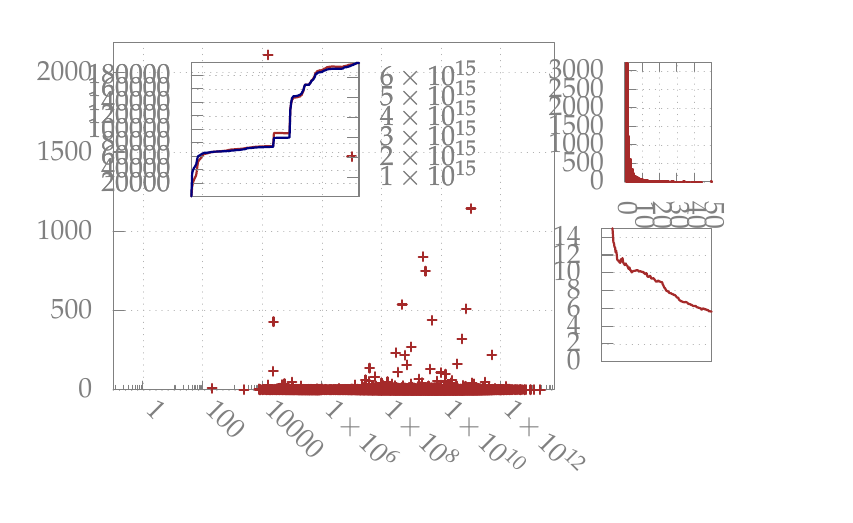
\begin{tikzpicture}[gnuplot, xscale=0.8, yscale=0.6]
%% generated with GNUPLOT 5.2p2 (Lua 5.3; terminal rev. 99, script rev. 102)
%% wo 11 jul 2018 12:06:38 CEST
\path (0.000,0.000) rectangle (12.500,8.750);
\gpcolor{color=gp lt color axes}
\gpsetlinetype{gp lt axes}
\gpsetdashtype{gp dt axes}
\gpsetlinewidth{0.50}
\draw[gp path] (1.196,1.085)--(8.197,1.085);
\gpcolor{rgb color={0.502,0.502,0.502}}
\gpsetlinetype{gp lt border}
\gpsetdashtype{gp dt solid}
\gpsetlinewidth{1.00}
\draw[gp path] (1.196,1.085)--(1.376,1.085);
\node[gp node right] at (1.012,1.085) {$0$};
\gpcolor{color=gp lt color axes}
\gpsetlinetype{gp lt axes}
\gpsetdashtype{gp dt axes}
\gpsetlinewidth{0.50}
\draw[gp path] (1.196,2.763)--(8.197,2.763);
\gpcolor{rgb color={0.502,0.502,0.502}}
\gpsetlinetype{gp lt border}
\gpsetdashtype{gp dt solid}
\gpsetlinewidth{1.00}
\draw[gp path] (1.196,2.763)--(1.376,2.763);
\node[gp node right] at (1.012,2.763) {$500$};
\gpcolor{color=gp lt color axes}
\gpsetlinetype{gp lt axes}
\gpsetdashtype{gp dt axes}
\gpsetlinewidth{0.50}
\draw[gp path] (1.196,4.441)--(8.197,4.441);
\gpcolor{rgb color={0.502,0.502,0.502}}
\gpsetlinetype{gp lt border}
\gpsetdashtype{gp dt solid}
\gpsetlinewidth{1.00}
\draw[gp path] (1.196,4.441)--(1.376,4.441);
\node[gp node right] at (1.012,4.441) {$1000$};
\gpcolor{color=gp lt color axes}
\gpsetlinetype{gp lt axes}
\gpsetdashtype{gp dt axes}
\gpsetlinewidth{0.50}
\draw[gp path] (1.196,6.119)--(8.197,6.119);
\gpcolor{rgb color={0.502,0.502,0.502}}
\gpsetlinetype{gp lt border}
\gpsetdashtype{gp dt solid}
\gpsetlinewidth{1.00}
\draw[gp path] (1.196,6.119)--(1.376,6.119);
\node[gp node right] at (1.012,6.119) {$1500$};
\gpcolor{color=gp lt color axes}
\gpsetlinetype{gp lt axes}
\gpsetdashtype{gp dt axes}
\gpsetlinewidth{0.50}
\draw[gp path] (1.196,7.797)--(8.197,7.797);
\gpcolor{rgb color={0.502,0.502,0.502}}
\gpsetlinetype{gp lt border}
\gpsetdashtype{gp dt solid}
\gpsetlinewidth{1.00}
\draw[gp path] (1.196,7.797)--(1.376,7.797);
\node[gp node right] at (1.012,7.797) {$2000$};
\draw[gp path] (1.233,1.088)--(1.233,1.178);
\draw[gp path] (1.367,1.088)--(1.367,1.178);
\draw[gp path] (1.448,1.088)--(1.448,1.178);
\draw[gp path] (1.505,1.088)--(1.505,1.178);
\draw[gp path] (1.550,1.088)--(1.550,1.178);
\draw[gp path] (1.587,1.088)--(1.587,1.178);
\draw[gp path] (1.618,1.088)--(1.618,1.178);
\draw[gp path] (1.645,1.088)--(1.645,1.178);
\gpcolor{color=gp lt color axes}
\gpsetlinetype{gp lt axes}
\gpsetdashtype{gp dt axes}
\gpsetlinewidth{0.50}
\draw[gp path] (1.669,1.088)--(1.669,8.441);
\gpcolor{rgb color={0.502,0.502,0.502}}
\gpsetlinetype{gp lt border}
\gpsetdashtype{gp dt solid}
\gpsetlinewidth{1.00}
\draw[gp path] (1.669,1.088)--(1.669,1.268);
\node[gp node left,rotate=-45] at (1.669,0.904) {$1$};
\draw[gp path] (2.180,1.088)--(2.180,1.178);
\draw[gp path] (2.314,1.088)--(2.314,1.178);
\draw[gp path] (2.394,1.088)--(2.394,1.178);
\draw[gp path] (2.452,1.088)--(2.452,1.178);
\draw[gp path] (2.497,1.088)--(2.497,1.178);
\draw[gp path] (2.534,1.088)--(2.534,1.178);
\draw[gp path] (2.565,1.088)--(2.565,1.178);
\draw[gp path] (2.592,1.088)--(2.592,1.178);
\gpcolor{color=gp lt color axes}
\gpsetlinetype{gp lt axes}
\gpsetdashtype{gp dt axes}
\gpsetlinewidth{0.50}
\draw[gp path] (2.616,1.088)--(2.616,8.441);
\gpcolor{rgb color={0.502,0.502,0.502}}
\gpsetlinetype{gp lt border}
\gpsetdashtype{gp dt solid}
\gpsetlinewidth{1.00}
\draw[gp path] (2.616,1.088)--(2.616,1.268);
\node[gp node left,rotate=-45] at (2.616,0.904) {$100$};
\draw[gp path] (3.127,1.088)--(3.127,1.178);
\draw[gp path] (3.261,1.088)--(3.261,1.178);
\draw[gp path] (3.341,1.088)--(3.341,1.178);
\draw[gp path] (3.399,1.088)--(3.399,1.178);
\draw[gp path] (3.444,1.088)--(3.444,1.178);
\draw[gp path] (3.481,1.088)--(3.481,1.178);
\draw[gp path] (3.512,1.088)--(3.512,1.178);
\draw[gp path] (3.539,1.088)--(3.539,1.178);
\gpcolor{color=gp lt color axes}
\gpsetlinetype{gp lt axes}
\gpsetdashtype{gp dt axes}
\gpsetlinewidth{0.50}
\draw[gp path] (3.563,1.088)--(3.563,8.441);
\gpcolor{rgb color={0.502,0.502,0.502}}
\gpsetlinetype{gp lt border}
\gpsetdashtype{gp dt solid}
\gpsetlinewidth{1.00}
\draw[gp path] (3.563,1.088)--(3.563,1.268);
\node[gp node left,rotate=-45] at (3.563,0.904) {$10000$};
\draw[gp path] (4.074,1.088)--(4.074,1.178);
\draw[gp path] (4.208,1.088)--(4.208,1.178);
\draw[gp path] (4.288,1.088)--(4.288,1.178);
\draw[gp path] (4.346,1.088)--(4.346,1.178);
\draw[gp path] (4.391,1.088)--(4.391,1.178);
\draw[gp path] (4.427,1.088)--(4.427,1.178);
\draw[gp path] (4.459,1.088)--(4.459,1.178);
\draw[gp path] (4.486,1.088)--(4.486,1.178);
\gpcolor{color=gp lt color axes}
\gpsetlinetype{gp lt axes}
\gpsetdashtype{gp dt axes}
\gpsetlinewidth{0.50}
\draw[gp path] (4.510,1.088)--(4.510,8.441);
\gpcolor{rgb color={0.502,0.502,0.502}}
\gpsetlinetype{gp lt border}
\gpsetdashtype{gp dt solid}
\gpsetlinewidth{1.00}
\draw[gp path] (4.510,1.088)--(4.510,1.268);
\node[gp node left,rotate=-45] at (4.510,0.904) {$1\times10^{6}$};
\draw[gp path] (5.021,1.088)--(5.021,1.178);
\draw[gp path] (5.154,1.088)--(5.154,1.178);
\draw[gp path] (5.235,1.088)--(5.235,1.178);
\draw[gp path] (5.292,1.088)--(5.292,1.178);
\draw[gp path] (5.337,1.088)--(5.337,1.178);
\draw[gp path] (5.374,1.088)--(5.374,1.178);
\draw[gp path] (5.405,1.088)--(5.405,1.178);
\draw[gp path] (5.433,1.088)--(5.433,1.178);
\gpcolor{color=gp lt color axes}
\gpsetlinetype{gp lt axes}
\gpsetdashtype{gp dt axes}
\gpsetlinewidth{0.50}
\draw[gp path] (5.457,1.088)--(5.457,8.441);
\gpcolor{rgb color={0.502,0.502,0.502}}
\gpsetlinetype{gp lt border}
\gpsetdashtype{gp dt solid}
\gpsetlinewidth{1.00}
\draw[gp path] (5.457,1.088)--(5.457,1.268);
\node[gp node left,rotate=-45] at (5.457,0.904) {$1\times10^{8}$};
\draw[gp path] (5.967,1.088)--(5.967,1.178);
\draw[gp path] (6.101,1.088)--(6.101,1.178);
\draw[gp path] (6.182,1.088)--(6.182,1.178);
\draw[gp path] (6.239,1.088)--(6.239,1.178);
\draw[gp path] (6.284,1.088)--(6.284,1.178);
\draw[gp path] (6.321,1.088)--(6.321,1.178);
\draw[gp path] (6.352,1.088)--(6.352,1.178);
\draw[gp path] (6.379,1.088)--(6.379,1.178);
\gpcolor{color=gp lt color axes}
\gpsetlinetype{gp lt axes}
\gpsetdashtype{gp dt axes}
\gpsetlinewidth{0.50}
\draw[gp path] (6.403,1.088)--(6.403,8.441);
\gpcolor{rgb color={0.502,0.502,0.502}}
\gpsetlinetype{gp lt border}
\gpsetdashtype{gp dt solid}
\gpsetlinewidth{1.00}
\draw[gp path] (6.403,1.088)--(6.403,1.268);
\node[gp node left,rotate=-45] at (6.403,0.904) {$1\times10^{10}$};
\draw[gp path] (6.914,1.088)--(6.914,1.178);
\draw[gp path] (7.048,1.088)--(7.048,1.178);
\draw[gp path] (7.128,1.088)--(7.128,1.178);
\draw[gp path] (7.186,1.088)--(7.186,1.178);
\draw[gp path] (7.231,1.088)--(7.231,1.178);
\draw[gp path] (7.268,1.088)--(7.268,1.178);
\draw[gp path] (7.299,1.088)--(7.299,1.178);
\draw[gp path] (7.326,1.088)--(7.326,1.178);
\gpcolor{color=gp lt color axes}
\gpsetlinetype{gp lt axes}
\gpsetdashtype{gp dt axes}
\gpsetlinewidth{0.50}
\draw[gp path] (7.350,1.088)--(7.350,8.261)--(7.350,8.441);
\gpcolor{rgb color={0.502,0.502,0.502}}
\gpsetlinetype{gp lt border}
\gpsetdashtype{gp dt solid}
\gpsetlinewidth{1.00}
\draw[gp path] (7.350,1.088)--(7.350,1.268);
\node[gp node left,rotate=-45] at (7.350,0.904) {$1\times10^{12}$};
\draw[gp path] (7.861,1.088)--(7.861,1.178);
\draw[gp path] (7.995,1.088)--(7.995,1.178);
\draw[gp path] (8.075,1.088)--(8.075,1.178);
\draw[gp path] (8.133,1.088)--(8.133,1.178);
\draw[gp path] (8.178,1.088)--(8.178,1.178);
\draw[gp path] (1.196,8.441)--(1.196,1.088)--(8.197,1.088)--(8.197,8.441)--cycle;
\gpcolor{rgb color={0.647,0.165,0.165}}
\gpsetlinewidth{2.00}
\gpsetpointsize{4.00}
\gppoint{gp mark 1}{(2.769,1.115)}
\gppoint{gp mark 1}{(3.274,1.088)}
\gppoint{gp mark 1}{(3.510,1.105)}
\gppoint{gp mark 1}{(3.520,1.088)}
\gppoint{gp mark 1}{(3.526,1.088)}
\gppoint{gp mark 1}{(3.536,1.088)}
\gppoint{gp mark 1}{(3.569,1.088)}
\gppoint{gp mark 1}{(3.580,1.088)}
\gppoint{gp mark 1}{(3.588,1.091)}
\gppoint{gp mark 1}{(3.604,1.088)}
\gppoint{gp mark 1}{(3.620,1.088)}
\gppoint{gp mark 1}{(3.632,1.088)}
\gppoint{gp mark 1}{(3.640,1.088)}
\gppoint{gp mark 1}{(3.650,1.088)}
\gppoint{gp mark 1}{(3.654,1.189)}
\gppoint{gp mark 1}{(3.658,8.173)}
\gppoint{gp mark 1}{(3.661,1.091)}
\gppoint{gp mark 1}{(3.667,1.088)}
\gppoint{gp mark 1}{(3.681,1.088)}
\gppoint{gp mark 1}{(3.689,1.091)}
\gppoint{gp mark 1}{(3.696,1.088)}
\gppoint{gp mark 1}{(3.702,1.088)}
\gppoint{gp mark 1}{(3.708,1.088)}
\gppoint{gp mark 1}{(3.718,1.088)}
\gppoint{gp mark 1}{(3.728,1.088)}
\gppoint{gp mark 1}{(3.736,1.088)}
\gppoint{gp mark 1}{(3.740,1.477)}
\gppoint{gp mark 1}{(3.743,2.528)}
\gppoint{gp mark 1}{(3.745,1.091)}
\gppoint{gp mark 1}{(3.752,1.088)}
\gppoint{gp mark 1}{(3.761,1.091)}
\gppoint{gp mark 1}{(3.765,1.091)}
\gppoint{gp mark 1}{(3.770,1.088)}
\gppoint{gp mark 1}{(3.777,1.088)}
\gppoint{gp mark 1}{(3.788,1.088)}
\gppoint{gp mark 1}{(3.792,1.088)}
\gppoint{gp mark 1}{(3.797,1.088)}
\gppoint{gp mark 1}{(3.799,1.095)}
\gppoint{gp mark 1}{(3.801,1.108)}
\gppoint{gp mark 1}{(3.804,1.091)}
\gppoint{gp mark 1}{(3.813,1.088)}
\gppoint{gp mark 1}{(3.819,1.088)}
\gppoint{gp mark 1}{(3.824,1.088)}
\gppoint{gp mark 1}{(3.828,1.088)}
\gppoint{gp mark 1}{(3.834,1.088)}
\gppoint{gp mark 1}{(3.839,1.088)}
\gppoint{gp mark 1}{(3.844,1.088)}
\gppoint{gp mark 1}{(3.846,1.098)}
\gppoint{gp mark 1}{(3.847,1.122)}
\gppoint{gp mark 1}{(3.850,1.088)}
\gppoint{gp mark 1}{(3.857,1.095)}
\gppoint{gp mark 1}{(3.860,1.088)}
\gppoint{gp mark 1}{(3.864,1.088)}
\gppoint{gp mark 1}{(3.872,1.088)}
\gppoint{gp mark 1}{(3.877,1.088)}
\gppoint{gp mark 1}{(3.883,1.091)}
\gppoint{gp mark 1}{(3.884,1.195)}
\gppoint{gp mark 1}{(3.886,1.088)}
\gppoint{gp mark 1}{(3.893,1.088)}
\gppoint{gp mark 1}{(3.896,1.088)}
\gppoint{gp mark 1}{(3.899,1.088)}
\gppoint{gp mark 1}{(3.903,1.091)}
\gppoint{gp mark 1}{(3.907,1.088)}
\gppoint{gp mark 1}{(3.911,1.088)}
\gppoint{gp mark 1}{(3.914,1.095)}
\gppoint{gp mark 1}{(3.915,1.165)}
\gppoint{gp mark 1}{(3.917,1.216)}
\gppoint{gp mark 1}{(3.921,1.088)}
\gppoint{gp mark 1}{(3.925,1.088)}
\gppoint{gp mark 1}{(3.927,1.088)}
\gppoint{gp mark 1}{(3.929,1.091)}
\gppoint{gp mark 1}{(3.933,1.088)}
\gppoint{gp mark 1}{(3.936,1.088)}
\gppoint{gp mark 1}{(3.940,1.088)}
\gppoint{gp mark 1}{(3.943,1.095)}
\gppoint{gp mark 1}{(3.944,1.088)}
\gppoint{gp mark 1}{(3.946,1.088)}
\gppoint{gp mark 1}{(3.949,1.088)}
\gppoint{gp mark 1}{(3.952,1.088)}
\gppoint{gp mark 1}{(3.954,1.088)}
\gppoint{gp mark 1}{(3.958,1.088)}
\gppoint{gp mark 1}{(3.961,1.091)}
\gppoint{gp mark 1}{(3.964,1.088)}
\gppoint{gp mark 1}{(3.967,1.115)}
\gppoint{gp mark 1}{(3.968,1.142)}
\gppoint{gp mark 1}{(3.971,1.095)}
\gppoint{gp mark 1}{(3.975,1.088)}
\gppoint{gp mark 1}{(3.976,1.088)}
\gppoint{gp mark 1}{(3.980,1.088)}
\gppoint{gp mark 1}{(3.984,1.088)}
\gppoint{gp mark 1}{(3.987,1.088)}
\gppoint{gp mark 1}{(3.989,1.088)}
\gppoint{gp mark 1}{(3.990,1.088)}
\gppoint{gp mark 1}{(3.992,1.091)}
\gppoint{gp mark 1}{(3.996,1.095)}
\gppoint{gp mark 1}{(3.998,1.088)}
\gppoint{gp mark 1}{(4.001,1.088)}
\gppoint{gp mark 1}{(4.004,1.088)}
\gppoint{gp mark 1}{(4.007,1.088)}
\gppoint{gp mark 1}{(4.009,1.101)}
\gppoint{gp mark 1}{(4.011,1.088)}
\gppoint{gp mark 1}{(4.014,1.088)}
\gppoint{gp mark 1}{(4.016,1.088)}
\gppoint{gp mark 1}{(4.018,1.088)}
\gppoint{gp mark 1}{(4.022,1.088)}
\gppoint{gp mark 1}{(4.024,1.088)}
\gppoint{gp mark 1}{(4.026,1.088)}
\gppoint{gp mark 1}{(4.027,1.101)}
\gppoint{gp mark 1}{(4.029,1.088)}
\gppoint{gp mark 1}{(4.032,1.091)}
\gppoint{gp mark 1}{(4.034,1.091)}
\gppoint{gp mark 1}{(4.036,1.246)}
\gppoint{gp mark 1}{(4.040,1.088)}
\gppoint{gp mark 1}{(4.042,1.088)}
\gppoint{gp mark 1}{(4.043,1.135)}
\gppoint{gp mark 1}{(4.045,1.088)}
\gppoint{gp mark 1}{(4.047,1.088)}
\gppoint{gp mark 1}{(4.049,1.088)}
\gppoint{gp mark 1}{(4.050,1.091)}
\gppoint{gp mark 1}{(4.053,1.088)}
\gppoint{gp mark 1}{(4.055,1.088)}
\gppoint{gp mark 1}{(4.057,1.091)}
\gppoint{gp mark 1}{(4.058,1.088)}
\gppoint{gp mark 1}{(4.060,1.088)}
\gppoint{gp mark 1}{(4.063,1.088)}
\gppoint{gp mark 1}{(4.065,1.088)}
\gppoint{gp mark 1}{(4.068,1.088)}
\gppoint{gp mark 1}{(4.070,1.088)}
\gppoint{gp mark 1}{(4.071,1.088)}
\gppoint{gp mark 1}{(4.073,1.088)}
\gppoint{gp mark 1}{(4.075,1.088)}
\gppoint{gp mark 1}{(4.078,1.088)}
\gppoint{gp mark 1}{(4.079,1.088)}
\gppoint{gp mark 1}{(4.082,1.088)}
\gppoint{gp mark 1}{(4.084,1.088)}
\gppoint{gp mark 1}{(4.086,1.088)}
\gppoint{gp mark 1}{(4.087,1.088)}
\gppoint{gp mark 1}{(4.088,1.088)}
\gppoint{gp mark 1}{(4.090,1.088)}
\gppoint{gp mark 1}{(4.091,1.095)}
\gppoint{gp mark 1}{(4.095,1.088)}
\gppoint{gp mark 1}{(4.096,1.088)}
\gppoint{gp mark 1}{(4.098,1.088)}
\gppoint{gp mark 1}{(4.100,1.088)}
\gppoint{gp mark 1}{(4.103,1.088)}
\gppoint{gp mark 1}{(4.103,1.088)}
\gppoint{gp mark 1}{(4.105,1.088)}
\gppoint{gp mark 1}{(4.108,1.091)}
\gppoint{gp mark 1}{(4.109,1.091)}
\gppoint{gp mark 1}{(4.111,1.088)}
\gppoint{gp mark 1}{(4.112,1.088)}
\gppoint{gp mark 1}{(4.114,1.088)}
\gppoint{gp mark 1}{(4.115,1.095)}
\gppoint{gp mark 1}{(4.116,1.088)}
\gppoint{gp mark 1}{(4.120,1.088)}
\gppoint{gp mark 1}{(4.122,1.088)}
\gppoint{gp mark 1}{(4.123,1.088)}
\gppoint{gp mark 1}{(4.126,1.088)}
\gppoint{gp mark 1}{(4.128,1.088)}
\gppoint{gp mark 1}{(4.130,1.088)}
\gppoint{gp mark 1}{(4.131,1.088)}
\gppoint{gp mark 1}{(4.133,1.088)}
\gppoint{gp mark 1}{(4.136,1.088)}
\gppoint{gp mark 1}{(4.137,1.095)}
\gppoint{gp mark 1}{(4.139,1.088)}
\gppoint{gp mark 1}{(4.141,1.088)}
\gppoint{gp mark 1}{(4.142,1.088)}
\gppoint{gp mark 1}{(4.144,1.088)}
\gppoint{gp mark 1}{(4.145,1.088)}
\gppoint{gp mark 1}{(4.146,1.091)}
\gppoint{gp mark 1}{(4.149,1.088)}
\gppoint{gp mark 1}{(4.150,1.088)}
\gppoint{gp mark 1}{(4.151,1.088)}
\gppoint{gp mark 1}{(4.153,1.088)}
\gppoint{gp mark 1}{(4.155,1.088)}
\gppoint{gp mark 1}{(4.156,1.091)}
\gppoint{gp mark 1}{(4.156,1.088)}
\gppoint{gp mark 1}{(4.158,1.088)}
\gppoint{gp mark 1}{(4.160,1.088)}
\gppoint{gp mark 1}{(4.162,1.088)}
\gppoint{gp mark 1}{(4.164,1.088)}
\gppoint{gp mark 1}{(4.164,1.095)}
\gppoint{gp mark 1}{(4.167,1.088)}
\gppoint{gp mark 1}{(4.169,1.088)}
\gppoint{gp mark 1}{(4.169,1.088)}
\gppoint{gp mark 1}{(4.172,1.088)}
\gppoint{gp mark 1}{(4.173,1.088)}
\gppoint{gp mark 1}{(4.173,1.095)}
\gppoint{gp mark 1}{(4.175,1.088)}
\gppoint{gp mark 1}{(4.176,1.088)}
\gppoint{gp mark 1}{(4.177,1.088)}
\gppoint{gp mark 1}{(4.179,1.169)}
\gppoint{gp mark 1}{(4.181,1.088)}
\gppoint{gp mark 1}{(4.182,1.088)}
\gppoint{gp mark 1}{(4.185,1.088)}
\gppoint{gp mark 1}{(4.186,1.088)}
\gppoint{gp mark 1}{(4.188,1.088)}
\gppoint{gp mark 1}{(4.189,1.088)}
\gppoint{gp mark 1}{(4.190,1.088)}
\gppoint{gp mark 1}{(4.193,1.088)}
\gppoint{gp mark 1}{(4.194,1.088)}
\gppoint{gp mark 1}{(4.196,1.088)}
\gppoint{gp mark 1}{(4.198,1.088)}
\gppoint{gp mark 1}{(4.200,1.088)}
\gppoint{gp mark 1}{(4.201,1.088)}
\gppoint{gp mark 1}{(4.202,1.088)}
\gppoint{gp mark 1}{(4.203,1.088)}
\gppoint{gp mark 1}{(4.204,1.088)}
\gppoint{gp mark 1}{(4.205,1.088)}
\gppoint{gp mark 1}{(4.208,1.088)}
\gppoint{gp mark 1}{(4.210,1.088)}
\gppoint{gp mark 1}{(4.211,1.091)}
\gppoint{gp mark 1}{(4.213,1.088)}
\gppoint{gp mark 1}{(4.214,1.088)}
\gppoint{gp mark 1}{(4.215,1.088)}
\gppoint{gp mark 1}{(4.217,1.088)}
\gppoint{gp mark 1}{(4.218,1.088)}
\gppoint{gp mark 1}{(4.220,1.088)}
\gppoint{gp mark 1}{(4.222,1.088)}
\gppoint{gp mark 1}{(4.224,1.088)}
\gppoint{gp mark 1}{(4.226,1.088)}
\gppoint{gp mark 1}{(4.228,1.088)}
\gppoint{gp mark 1}{(4.229,1.088)}
\gppoint{gp mark 1}{(4.231,1.091)}
\gppoint{gp mark 1}{(4.232,1.088)}
\gppoint{gp mark 1}{(4.233,1.088)}
\gppoint{gp mark 1}{(4.234,1.088)}
\gppoint{gp mark 1}{(4.236,1.088)}
\gppoint{gp mark 1}{(4.238,1.088)}
\gppoint{gp mark 1}{(4.239,1.088)}
\gppoint{gp mark 1}{(4.240,1.088)}
\gppoint{gp mark 1}{(4.242,1.088)}
\gppoint{gp mark 1}{(4.243,1.088)}
\gppoint{gp mark 1}{(4.244,1.088)}
\gppoint{gp mark 1}{(4.245,1.088)}
\gppoint{gp mark 1}{(4.247,1.088)}
\gppoint{gp mark 1}{(4.248,1.088)}
\gppoint{gp mark 1}{(4.250,1.088)}
\gppoint{gp mark 1}{(4.251,1.088)}
\gppoint{gp mark 1}{(4.252,1.088)}
\gppoint{gp mark 1}{(4.254,1.088)}
\gppoint{gp mark 1}{(4.256,1.088)}
\gppoint{gp mark 1}{(4.257,1.088)}
\gppoint{gp mark 1}{(4.258,1.088)}
\gppoint{gp mark 1}{(4.259,1.088)}
\gppoint{gp mark 1}{(4.260,1.088)}
\gppoint{gp mark 1}{(4.262,1.088)}
\gppoint{gp mark 1}{(4.263,1.088)}
\gppoint{gp mark 1}{(4.265,1.088)}
\gppoint{gp mark 1}{(4.266,1.088)}
\gppoint{gp mark 1}{(4.268,1.088)}
\gppoint{gp mark 1}{(4.269,1.088)}
\gppoint{gp mark 1}{(4.271,1.088)}
\gppoint{gp mark 1}{(4.272,1.088)}
\gppoint{gp mark 1}{(4.273,1.088)}
\gppoint{gp mark 1}{(4.274,1.088)}
\gppoint{gp mark 1}{(4.276,1.088)}
\gppoint{gp mark 1}{(4.278,1.088)}
\gppoint{gp mark 1}{(4.279,1.088)}
\gppoint{gp mark 1}{(4.280,1.088)}
\gppoint{gp mark 1}{(4.281,1.088)}
\gppoint{gp mark 1}{(4.282,1.088)}
\gppoint{gp mark 1}{(4.284,1.088)}
\gppoint{gp mark 1}{(4.285,1.088)}
\gppoint{gp mark 1}{(4.287,1.088)}
\gppoint{gp mark 1}{(4.289,1.088)}
\gppoint{gp mark 1}{(4.290,1.088)}
\gppoint{gp mark 1}{(4.292,1.088)}
\gppoint{gp mark 1}{(4.293,1.088)}
\gppoint{gp mark 1}{(4.294,1.088)}
\gppoint{gp mark 1}{(4.295,1.088)}
\gppoint{gp mark 1}{(4.296,1.088)}
\gppoint{gp mark 1}{(4.298,1.088)}
\gppoint{gp mark 1}{(4.298,1.091)}
\gppoint{gp mark 1}{(4.300,1.088)}
\gppoint{gp mark 1}{(4.301,1.088)}
\gppoint{gp mark 1}{(4.302,1.088)}
\gppoint{gp mark 1}{(4.303,1.088)}
\gppoint{gp mark 1}{(4.304,1.088)}
\gppoint{gp mark 1}{(4.306,1.088)}
\gppoint{gp mark 1}{(4.307,1.091)}
\gppoint{gp mark 1}{(4.309,1.088)}
\gppoint{gp mark 1}{(4.310,1.088)}
\gppoint{gp mark 1}{(4.311,1.088)}
\gppoint{gp mark 1}{(4.312,1.088)}
\gppoint{gp mark 1}{(4.313,1.088)}
\gppoint{gp mark 1}{(4.314,1.088)}
\gppoint{gp mark 1}{(4.315,1.088)}
\gppoint{gp mark 1}{(4.316,1.088)}
\gppoint{gp mark 1}{(4.317,1.088)}
\gppoint{gp mark 1}{(4.319,1.088)}
\gppoint{gp mark 1}{(4.320,1.088)}
\gppoint{gp mark 1}{(4.321,1.088)}
\gppoint{gp mark 1}{(4.324,1.088)}
\gppoint{gp mark 1}{(4.325,1.088)}
\gppoint{gp mark 1}{(4.325,1.088)}
\gppoint{gp mark 1}{(4.327,1.088)}
\gppoint{gp mark 1}{(4.328,1.088)}
\gppoint{gp mark 1}{(4.329,1.088)}
\gppoint{gp mark 1}{(4.331,1.088)}
\gppoint{gp mark 1}{(4.332,1.091)}
\gppoint{gp mark 1}{(4.333,1.088)}
\gppoint{gp mark 1}{(4.334,1.088)}
\gppoint{gp mark 1}{(4.336,1.088)}
\gppoint{gp mark 1}{(4.337,1.088)}
\gppoint{gp mark 1}{(4.338,1.088)}
\gppoint{gp mark 1}{(4.339,1.088)}
\gppoint{gp mark 1}{(4.340,1.091)}
\gppoint{gp mark 1}{(4.342,1.088)}
\gppoint{gp mark 1}{(4.343,1.091)}
\gppoint{gp mark 1}{(4.345,1.088)}
\gppoint{gp mark 1}{(4.345,1.088)}
\gppoint{gp mark 1}{(4.347,1.088)}
\gppoint{gp mark 1}{(4.348,1.088)}
\gppoint{gp mark 1}{(4.349,1.088)}
\gppoint{gp mark 1}{(4.351,1.088)}
\gppoint{gp mark 1}{(4.352,1.088)}
\gppoint{gp mark 1}{(4.354,1.088)}
\gppoint{gp mark 1}{(4.354,1.088)}
\gppoint{gp mark 1}{(4.355,1.088)}
\gppoint{gp mark 1}{(4.357,1.088)}
\gppoint{gp mark 1}{(4.358,1.088)}
\gppoint{gp mark 1}{(4.359,1.088)}
\gppoint{gp mark 1}{(4.361,1.088)}
\gppoint{gp mark 1}{(4.361,1.088)}
\gppoint{gp mark 1}{(4.362,1.088)}
\gppoint{gp mark 1}{(4.364,1.088)}
\gppoint{gp mark 1}{(4.365,1.088)}
\gppoint{gp mark 1}{(4.366,1.088)}
\gppoint{gp mark 1}{(4.368,1.088)}
\gppoint{gp mark 1}{(4.369,1.088)}
\gppoint{gp mark 1}{(4.370,1.088)}
\gppoint{gp mark 1}{(4.371,1.088)}
\gppoint{gp mark 1}{(4.372,1.088)}
\gppoint{gp mark 1}{(4.374,1.088)}
\gppoint{gp mark 1}{(4.375,1.088)}
\gppoint{gp mark 1}{(4.377,1.088)}
\gppoint{gp mark 1}{(4.378,1.088)}
\gppoint{gp mark 1}{(4.380,1.088)}
\gppoint{gp mark 1}{(4.381,1.088)}
\gppoint{gp mark 1}{(4.382,1.088)}
\gppoint{gp mark 1}{(4.382,1.088)}
\gppoint{gp mark 1}{(4.384,1.088)}
\gppoint{gp mark 1}{(4.384,1.088)}
\gppoint{gp mark 1}{(4.385,1.088)}
\gppoint{gp mark 1}{(4.386,1.088)}
\gppoint{gp mark 1}{(4.387,1.088)}
\gppoint{gp mark 1}{(4.388,1.088)}
\gppoint{gp mark 1}{(4.389,1.088)}
\gppoint{gp mark 1}{(4.390,1.088)}
\gppoint{gp mark 1}{(4.391,1.088)}
\gppoint{gp mark 1}{(4.392,1.088)}
\gppoint{gp mark 1}{(4.394,1.088)}
\gppoint{gp mark 1}{(4.395,1.088)}
\gppoint{gp mark 1}{(4.396,1.088)}
\gppoint{gp mark 1}{(4.396,1.088)}
\gppoint{gp mark 1}{(4.398,1.088)}
\gppoint{gp mark 1}{(4.399,1.088)}
\gppoint{gp mark 1}{(4.400,1.088)}
\gppoint{gp mark 1}{(4.402,1.088)}
\gppoint{gp mark 1}{(4.402,1.088)}
\gppoint{gp mark 1}{(4.404,1.088)}
\gppoint{gp mark 1}{(4.405,1.088)}
\gppoint{gp mark 1}{(4.406,1.088)}
\gppoint{gp mark 1}{(4.407,1.088)}
\gppoint{gp mark 1}{(4.408,1.088)}
\gppoint{gp mark 1}{(4.410,1.088)}
\gppoint{gp mark 1}{(4.410,1.088)}
\gppoint{gp mark 1}{(4.412,1.088)}
\gppoint{gp mark 1}{(4.412,1.088)}
\gppoint{gp mark 1}{(4.413,1.088)}
\gppoint{gp mark 1}{(4.414,1.088)}
\gppoint{gp mark 1}{(4.415,1.088)}
\gppoint{gp mark 1}{(4.417,1.088)}
\gppoint{gp mark 1}{(4.418,1.088)}
\gppoint{gp mark 1}{(4.418,1.088)}
\gppoint{gp mark 1}{(4.419,1.088)}
\gppoint{gp mark 1}{(4.420,1.088)}
\gppoint{gp mark 1}{(4.421,1.088)}
\gppoint{gp mark 1}{(4.422,1.088)}
\gppoint{gp mark 1}{(4.423,1.088)}
\gppoint{gp mark 1}{(4.423,1.088)}
\gppoint{gp mark 1}{(4.425,1.088)}
\gppoint{gp mark 1}{(4.426,1.088)}
\gppoint{gp mark 1}{(4.426,1.088)}
\gppoint{gp mark 1}{(4.428,1.088)}
\gppoint{gp mark 1}{(4.428,1.088)}
\gppoint{gp mark 1}{(4.430,1.088)}
\gppoint{gp mark 1}{(4.430,1.088)}
\gppoint{gp mark 1}{(4.432,1.088)}
\gppoint{gp mark 1}{(4.433,1.088)}
\gppoint{gp mark 1}{(4.435,1.088)}
\gppoint{gp mark 1}{(4.435,1.088)}
\gppoint{gp mark 1}{(4.436,1.108)}
\gppoint{gp mark 1}{(4.437,1.088)}
\gppoint{gp mark 1}{(4.439,1.088)}
\gppoint{gp mark 1}{(4.440,1.088)}
\gppoint{gp mark 1}{(4.440,1.088)}
\gppoint{gp mark 1}{(4.442,1.088)}
\gppoint{gp mark 1}{(4.443,1.088)}
\gppoint{gp mark 1}{(4.444,1.088)}
\gppoint{gp mark 1}{(4.444,1.088)}
\gppoint{gp mark 1}{(4.446,1.088)}
\gppoint{gp mark 1}{(4.447,1.088)}
\gppoint{gp mark 1}{(4.447,1.088)}
\gppoint{gp mark 1}{(4.449,1.088)}
\gppoint{gp mark 1}{(4.449,1.088)}
\gppoint{gp mark 1}{(4.450,1.088)}
\gppoint{gp mark 1}{(4.451,1.088)}
\gppoint{gp mark 1}{(4.453,1.088)}
\gppoint{gp mark 1}{(4.453,1.088)}
\gppoint{gp mark 1}{(4.455,1.088)}
\gppoint{gp mark 1}{(4.455,1.088)}
\gppoint{gp mark 1}{(4.456,1.088)}
\gppoint{gp mark 1}{(4.458,1.091)}
\gppoint{gp mark 1}{(4.458,1.088)}
\gppoint{gp mark 1}{(4.459,1.088)}
\gppoint{gp mark 1}{(4.460,1.088)}
\gppoint{gp mark 1}{(4.460,1.088)}
\gppoint{gp mark 1}{(4.462,1.088)}
\gppoint{gp mark 1}{(4.462,1.088)}
\gppoint{gp mark 1}{(4.464,1.088)}
\gppoint{gp mark 1}{(4.464,1.088)}
\gppoint{gp mark 1}{(4.465,1.088)}
\gppoint{gp mark 1}{(4.466,1.088)}
\gppoint{gp mark 1}{(4.468,1.091)}
\gppoint{gp mark 1}{(4.468,1.088)}
\gppoint{gp mark 1}{(4.469,1.088)}
\gppoint{gp mark 1}{(4.470,1.088)}
\gppoint{gp mark 1}{(4.471,1.088)}
\gppoint{gp mark 1}{(4.472,1.088)}
\gppoint{gp mark 1}{(4.474,1.088)}
\gppoint{gp mark 1}{(4.474,1.091)}
\gppoint{gp mark 1}{(4.476,1.088)}
\gppoint{gp mark 1}{(4.478,1.088)}
\gppoint{gp mark 1}{(4.478,1.088)}
\gppoint{gp mark 1}{(4.480,1.088)}
\gppoint{gp mark 1}{(4.481,1.088)}
\gppoint{gp mark 1}{(4.482,1.088)}
\gppoint{gp mark 1}{(4.483,1.088)}
\gppoint{gp mark 1}{(4.485,1.088)}
\gppoint{gp mark 1}{(4.485,1.088)}
\gppoint{gp mark 1}{(4.487,1.088)}
\gppoint{gp mark 1}{(4.489,1.091)}
\gppoint{gp mark 1}{(4.491,1.091)}
\gppoint{gp mark 1}{(4.493,1.088)}
\gppoint{gp mark 1}{(4.494,1.088)}
\gppoint{gp mark 1}{(4.496,1.091)}
\gppoint{gp mark 1}{(4.496,1.088)}
\gppoint{gp mark 1}{(4.498,1.088)}
\gppoint{gp mark 1}{(4.500,1.088)}
\gppoint{gp mark 1}{(4.500,1.088)}
\gppoint{gp mark 1}{(4.501,1.088)}
\gppoint{gp mark 1}{(4.503,1.088)}
\gppoint{gp mark 1}{(4.505,1.088)}
\gppoint{gp mark 1}{(4.506,1.101)}
\gppoint{gp mark 1}{(4.508,1.088)}
\gppoint{gp mark 1}{(4.511,1.088)}
\gppoint{gp mark 1}{(4.515,1.088)}
\gppoint{gp mark 1}{(4.523,1.088)}
\gppoint{gp mark 1}{(4.544,1.088)}
\gppoint{gp mark 1}{(4.553,1.088)}
\gppoint{gp mark 1}{(4.567,1.091)}
\gppoint{gp mark 1}{(4.583,1.088)}
\gppoint{gp mark 1}{(4.594,1.088)}
\gppoint{gp mark 1}{(4.611,1.088)}
\gppoint{gp mark 1}{(4.627,1.088)}
\gppoint{gp mark 1}{(4.633,1.088)}
\gppoint{gp mark 1}{(4.635,1.088)}
\gppoint{gp mark 1}{(4.647,1.088)}
\gppoint{gp mark 1}{(4.654,1.088)}
\gppoint{gp mark 1}{(4.665,1.088)}
\gppoint{gp mark 1}{(4.676,1.088)}
\gppoint{gp mark 1}{(4.686,1.088)}
\gppoint{gp mark 1}{(4.695,1.088)}
\gppoint{gp mark 1}{(4.708,1.095)}
\gppoint{gp mark 1}{(4.714,1.088)}
\gppoint{gp mark 1}{(4.723,1.088)}
\gppoint{gp mark 1}{(4.728,1.088)}
\gppoint{gp mark 1}{(4.734,1.088)}
\gppoint{gp mark 1}{(4.737,1.088)}
\gppoint{gp mark 1}{(4.749,1.091)}
\gppoint{gp mark 1}{(4.760,1.088)}
\gppoint{gp mark 1}{(4.769,1.088)}
\gppoint{gp mark 1}{(4.775,1.088)}
\gppoint{gp mark 1}{(4.779,1.088)}
\gppoint{gp mark 1}{(4.785,1.088)}
\gppoint{gp mark 1}{(4.786,1.115)}
\gppoint{gp mark 1}{(4.792,1.088)}
\gppoint{gp mark 1}{(4.795,1.088)}
\gppoint{gp mark 1}{(4.797,1.088)}
\gppoint{gp mark 1}{(4.808,1.088)}
\gppoint{gp mark 1}{(4.814,1.088)}
\gppoint{gp mark 1}{(4.820,1.088)}
\gppoint{gp mark 1}{(4.826,1.088)}
\gppoint{gp mark 1}{(4.831,1.088)}
\gppoint{gp mark 1}{(4.833,1.088)}
\gppoint{gp mark 1}{(4.839,1.088)}
\gppoint{gp mark 1}{(4.841,1.088)}
\gppoint{gp mark 1}{(4.847,1.088)}
\gppoint{gp mark 1}{(4.853,1.088)}
\gppoint{gp mark 1}{(4.856,1.088)}
\gppoint{gp mark 1}{(4.860,1.088)}
\gppoint{gp mark 1}{(4.865,1.088)}
\gppoint{gp mark 1}{(4.872,1.088)}
\gppoint{gp mark 1}{(4.875,1.088)}
\gppoint{gp mark 1}{(4.878,1.091)}
\gppoint{gp mark 1}{(4.883,1.088)}
\gppoint{gp mark 1}{(4.887,1.088)}
\gppoint{gp mark 1}{(4.889,1.088)}
\gppoint{gp mark 1}{(4.894,1.088)}
\gppoint{gp mark 1}{(4.896,1.088)}
\gppoint{gp mark 1}{(4.900,1.088)}
\gppoint{gp mark 1}{(4.904,1.088)}
\gppoint{gp mark 1}{(4.905,1.088)}
\gppoint{gp mark 1}{(4.907,1.088)}
\gppoint{gp mark 1}{(4.911,1.088)}
\gppoint{gp mark 1}{(4.915,1.088)}
\gppoint{gp mark 1}{(4.919,1.088)}
\gppoint{gp mark 1}{(4.924,1.088)}
\gppoint{gp mark 1}{(4.927,1.088)}
\gppoint{gp mark 1}{(4.928,1.091)}
\gppoint{gp mark 1}{(4.932,1.088)}
\gppoint{gp mark 1}{(4.933,1.088)}
\gppoint{gp mark 1}{(4.937,1.088)}
\gppoint{gp mark 1}{(4.940,1.088)}
\gppoint{gp mark 1}{(4.946,1.088)}
\gppoint{gp mark 1}{(4.949,1.088)}
\gppoint{gp mark 1}{(4.953,1.088)}
\gppoint{gp mark 1}{(4.955,1.088)}
\gppoint{gp mark 1}{(4.957,1.088)}
\gppoint{gp mark 1}{(4.958,1.088)}
\gppoint{gp mark 1}{(4.960,1.088)}
\gppoint{gp mark 1}{(4.961,1.088)}
\gppoint{gp mark 1}{(4.962,1.088)}
\gppoint{gp mark 1}{(4.964,1.088)}
\gppoint{gp mark 1}{(4.967,1.088)}
\gppoint{gp mark 1}{(4.971,1.088)}
\gppoint{gp mark 1}{(4.973,1.088)}
\gppoint{gp mark 1}{(4.975,1.098)}
\gppoint{gp mark 1}{(4.978,1.088)}
\gppoint{gp mark 1}{(4.979,1.088)}
\gppoint{gp mark 1}{(4.979,1.088)}
\gppoint{gp mark 1}{(4.981,1.088)}
\gppoint{gp mark 1}{(4.981,1.088)}
\gppoint{gp mark 1}{(4.983,6.021)}
\gppoint{gp mark 1}{(4.984,1.088)}
\gppoint{gp mark 1}{(4.986,1.088)}
\gppoint{gp mark 1}{(4.987,1.088)}
\gppoint{gp mark 1}{(4.987,1.105)}
\gppoint{gp mark 1}{(4.989,1.088)}
\gppoint{gp mark 1}{(4.990,1.091)}
\gppoint{gp mark 1}{(4.991,1.088)}
\gppoint{gp mark 1}{(4.993,1.088)}
\gppoint{gp mark 1}{(4.995,1.088)}
\gppoint{gp mark 1}{(4.997,1.088)}
\gppoint{gp mark 1}{(4.999,1.088)}
\gppoint{gp mark 1}{(5.001,1.088)}
\gppoint{gp mark 1}{(5.003,1.088)}
\gppoint{gp mark 1}{(5.004,1.088)}
\gppoint{gp mark 1}{(5.005,1.088)}
\gppoint{gp mark 1}{(5.008,1.088)}
\gppoint{gp mark 1}{(5.011,1.088)}
\gppoint{gp mark 1}{(5.014,1.091)}
\gppoint{gp mark 1}{(5.015,1.088)}
\gppoint{gp mark 1}{(5.017,1.088)}
\gppoint{gp mark 1}{(5.018,1.095)}
\gppoint{gp mark 1}{(5.019,1.088)}
\gppoint{gp mark 1}{(5.021,1.088)}
\gppoint{gp mark 1}{(5.023,1.088)}
\gppoint{gp mark 1}{(5.024,1.088)}
\gppoint{gp mark 1}{(5.027,1.088)}
\gppoint{gp mark 1}{(5.029,1.088)}
\gppoint{gp mark 1}{(5.031,1.088)}
\gppoint{gp mark 1}{(5.032,1.088)}
\gppoint{gp mark 1}{(5.034,1.088)}
\gppoint{gp mark 1}{(5.034,1.088)}
\gppoint{gp mark 1}{(5.037,1.189)}
\gppoint{gp mark 1}{(5.039,1.088)}
\gppoint{gp mark 1}{(5.042,1.088)}
\gppoint{gp mark 1}{(5.044,1.088)}
\gppoint{gp mark 1}{(5.045,1.088)}
\gppoint{gp mark 1}{(5.047,1.088)}
\gppoint{gp mark 1}{(5.049,1.088)}
\gppoint{gp mark 1}{(5.050,1.088)}
\gppoint{gp mark 1}{(5.051,1.088)}
\gppoint{gp mark 1}{(5.054,1.088)}
\gppoint{gp mark 1}{(5.055,1.088)}
\gppoint{gp mark 1}{(5.058,1.088)}
\gppoint{gp mark 1}{(5.059,1.088)}
\gppoint{gp mark 1}{(5.061,1.088)}
\gppoint{gp mark 1}{(5.062,1.091)}
\gppoint{gp mark 1}{(5.064,1.088)}
\gppoint{gp mark 1}{(5.064,1.091)}
\gppoint{gp mark 1}{(5.066,1.088)}
\gppoint{gp mark 1}{(5.068,1.088)}
\gppoint{gp mark 1}{(5.070,1.088)}
\gppoint{gp mark 1}{(5.071,1.088)}
\gppoint{gp mark 1}{(5.073,1.088)}
\gppoint{gp mark 1}{(5.075,1.088)}
\gppoint{gp mark 1}{(5.076,1.088)}
\gppoint{gp mark 1}{(5.077,1.088)}
\gppoint{gp mark 1}{(5.078,1.095)}
\gppoint{gp mark 1}{(5.079,1.088)}
\gppoint{gp mark 1}{(5.080,1.088)}
\gppoint{gp mark 1}{(5.081,1.088)}
\gppoint{gp mark 1}{(5.083,1.088)}
\gppoint{gp mark 1}{(5.084,1.088)}
\gppoint{gp mark 1}{(5.085,1.088)}
\gppoint{gp mark 1}{(5.088,1.088)}
\gppoint{gp mark 1}{(5.090,1.088)}
\gppoint{gp mark 1}{(5.090,1.095)}
\gppoint{gp mark 1}{(5.092,1.088)}
\gppoint{gp mark 1}{(5.093,1.088)}
\gppoint{gp mark 1}{(5.095,1.088)}
\gppoint{gp mark 1}{(5.096,1.088)}
\gppoint{gp mark 1}{(5.098,1.088)}
\gppoint{gp mark 1}{(5.100,1.088)}
\gppoint{gp mark 1}{(5.101,1.088)}
\gppoint{gp mark 1}{(5.102,1.088)}
\gppoint{gp mark 1}{(5.104,1.088)}
\gppoint{gp mark 1}{(5.104,1.088)}
\gppoint{gp mark 1}{(5.106,1.088)}
\gppoint{gp mark 1}{(5.107,1.088)}
\gppoint{gp mark 1}{(5.108,1.088)}
\gppoint{gp mark 1}{(5.109,1.088)}
\gppoint{gp mark 1}{(5.111,1.088)}
\gppoint{gp mark 1}{(5.112,1.088)}
\gppoint{gp mark 1}{(5.113,1.088)}
\gppoint{gp mark 1}{(5.113,1.088)}
\gppoint{gp mark 1}{(5.115,1.088)}
\gppoint{gp mark 1}{(5.116,1.088)}
\gppoint{gp mark 1}{(5.117,1.088)}
\gppoint{gp mark 1}{(5.119,1.088)}
\gppoint{gp mark 1}{(5.120,1.088)}
\gppoint{gp mark 1}{(5.121,1.088)}
\gppoint{gp mark 1}{(5.122,1.088)}
\gppoint{gp mark 1}{(5.123,1.088)}
\gppoint{gp mark 1}{(5.124,1.088)}
\gppoint{gp mark 1}{(5.124,1.088)}
\gppoint{gp mark 1}{(5.125,1.088)}
\gppoint{gp mark 1}{(5.125,1.088)}
\gppoint{gp mark 1}{(5.126,1.088)}
\gppoint{gp mark 1}{(5.126,1.088)}
\gppoint{gp mark 1}{(5.127,1.088)}
\gppoint{gp mark 1}{(5.128,1.088)}
\gppoint{gp mark 1}{(5.129,1.088)}
\gppoint{gp mark 1}{(5.130,1.088)}
\gppoint{gp mark 1}{(5.130,1.088)}
\gppoint{gp mark 1}{(5.131,1.088)}
\gppoint{gp mark 1}{(5.132,1.088)}
\gppoint{gp mark 1}{(5.133,1.088)}
\gppoint{gp mark 1}{(5.133,1.088)}
\gppoint{gp mark 1}{(5.134,1.088)}
\gppoint{gp mark 1}{(5.134,1.088)}
\gppoint{gp mark 1}{(5.135,1.088)}
\gppoint{gp mark 1}{(5.136,1.088)}
\gppoint{gp mark 1}{(5.138,1.088)}
\gppoint{gp mark 1}{(5.138,1.088)}
\gppoint{gp mark 1}{(5.140,1.088)}
\gppoint{gp mark 1}{(5.141,1.088)}
\gppoint{gp mark 1}{(5.142,1.088)}
\gppoint{gp mark 1}{(5.143,1.088)}
\gppoint{gp mark 1}{(5.144,1.088)}
\gppoint{gp mark 1}{(5.144,1.088)}
\gppoint{gp mark 1}{(5.145,1.182)}
\gppoint{gp mark 1}{(5.147,1.088)}
\gppoint{gp mark 1}{(5.147,1.088)}
\gppoint{gp mark 1}{(5.148,1.088)}
\gppoint{gp mark 1}{(5.149,1.088)}
\gppoint{gp mark 1}{(5.150,1.088)}
\gppoint{gp mark 1}{(5.152,1.088)}
\gppoint{gp mark 1}{(5.153,1.098)}
\gppoint{gp mark 1}{(5.154,1.088)}
\gppoint{gp mark 1}{(5.155,1.088)}
\gppoint{gp mark 1}{(5.156,1.088)}
\gppoint{gp mark 1}{(5.157,1.088)}
\gppoint{gp mark 1}{(5.158,1.088)}
\gppoint{gp mark 1}{(5.159,1.091)}
\gppoint{gp mark 1}{(5.160,1.088)}
\gppoint{gp mark 1}{(5.160,1.088)}
\gppoint{gp mark 1}{(5.161,1.142)}
\gppoint{gp mark 1}{(5.162,1.088)}
\gppoint{gp mark 1}{(5.163,1.088)}
\gppoint{gp mark 1}{(5.164,1.088)}
\gppoint{gp mark 1}{(5.164,1.088)}
\gppoint{gp mark 1}{(5.166,1.088)}
\gppoint{gp mark 1}{(5.167,1.088)}
\gppoint{gp mark 1}{(5.168,1.088)}
\gppoint{gp mark 1}{(5.169,1.088)}
\gppoint{gp mark 1}{(5.170,1.088)}
\gppoint{gp mark 1}{(5.171,1.088)}
\gppoint{gp mark 1}{(5.171,1.088)}
\gppoint{gp mark 1}{(5.172,1.088)}
\gppoint{gp mark 1}{(5.173,1.088)}
\gppoint{gp mark 1}{(5.174,1.088)}
\gppoint{gp mark 1}{(5.175,1.088)}
\gppoint{gp mark 1}{(5.176,1.088)}
\gppoint{gp mark 1}{(5.177,1.088)}
\gppoint{gp mark 1}{(5.178,1.088)}
\gppoint{gp mark 1}{(5.178,1.088)}
\gppoint{gp mark 1}{(5.179,1.088)}
\gppoint{gp mark 1}{(5.179,1.088)}
\gppoint{gp mark 1}{(5.181,1.088)}
\gppoint{gp mark 1}{(5.182,1.088)}
\gppoint{gp mark 1}{(5.183,1.088)}
\gppoint{gp mark 1}{(5.184,1.088)}
\gppoint{gp mark 1}{(5.185,1.088)}
\gppoint{gp mark 1}{(5.186,1.088)}
\gppoint{gp mark 1}{(5.186,1.088)}
\gppoint{gp mark 1}{(5.187,1.088)}
\gppoint{gp mark 1}{(5.187,1.088)}
\gppoint{gp mark 1}{(5.188,1.088)}
\gppoint{gp mark 1}{(5.189,1.088)}
\gppoint{gp mark 1}{(5.190,1.088)}
\gppoint{gp mark 1}{(5.191,1.088)}
\gppoint{gp mark 1}{(5.192,1.088)}
\gppoint{gp mark 1}{(5.192,1.088)}
\gppoint{gp mark 1}{(5.193,1.088)}
\gppoint{gp mark 1}{(5.194,1.088)}
\gppoint{gp mark 1}{(5.194,1.088)}
\gppoint{gp mark 1}{(5.195,1.091)}
\gppoint{gp mark 1}{(5.196,1.088)}
\gppoint{gp mark 1}{(5.197,1.088)}
\gppoint{gp mark 1}{(5.198,1.088)}
\gppoint{gp mark 1}{(5.199,1.088)}
\gppoint{gp mark 1}{(5.200,1.088)}
\gppoint{gp mark 1}{(5.201,1.088)}
\gppoint{gp mark 1}{(5.201,1.088)}
\gppoint{gp mark 1}{(5.202,1.088)}
\gppoint{gp mark 1}{(5.202,1.296)}
\gppoint{gp mark 1}{(5.203,1.088)}
\gppoint{gp mark 1}{(5.204,1.088)}
\gppoint{gp mark 1}{(5.206,1.101)}
\gppoint{gp mark 1}{(5.206,1.088)}
\gppoint{gp mark 1}{(5.207,1.088)}
\gppoint{gp mark 1}{(5.208,1.088)}
\gppoint{gp mark 1}{(5.208,1.088)}
\gppoint{gp mark 1}{(5.209,1.088)}
\gppoint{gp mark 1}{(5.209,1.088)}
\gppoint{gp mark 1}{(5.210,1.088)}
\gppoint{gp mark 1}{(5.211,1.088)}
\gppoint{gp mark 1}{(5.212,1.088)}
\gppoint{gp mark 1}{(5.214,1.088)}
\gppoint{gp mark 1}{(5.214,1.122)}
\gppoint{gp mark 1}{(5.215,1.088)}
\gppoint{gp mark 1}{(5.216,1.199)}
\gppoint{gp mark 1}{(5.217,1.088)}
\gppoint{gp mark 1}{(5.218,1.088)}
\gppoint{gp mark 1}{(5.219,1.088)}
\gppoint{gp mark 1}{(5.220,1.088)}
\gppoint{gp mark 1}{(5.221,1.088)}
\gppoint{gp mark 1}{(5.222,1.088)}
\gppoint{gp mark 1}{(5.222,1.088)}
\gppoint{gp mark 1}{(5.223,1.088)}
\gppoint{gp mark 1}{(5.224,1.088)}
\gppoint{gp mark 1}{(5.225,1.088)}
\gppoint{gp mark 1}{(5.225,1.088)}
\gppoint{gp mark 1}{(5.226,1.091)}
\gppoint{gp mark 1}{(5.227,1.088)}
\gppoint{gp mark 1}{(5.228,1.088)}
\gppoint{gp mark 1}{(5.228,1.088)}
\gppoint{gp mark 1}{(5.229,1.088)}
\gppoint{gp mark 1}{(5.230,1.088)}
\gppoint{gp mark 1}{(5.231,1.088)}
\gppoint{gp mark 1}{(5.233,1.088)}
\gppoint{gp mark 1}{(5.233,1.088)}
\gppoint{gp mark 1}{(5.234,1.088)}
\gppoint{gp mark 1}{(5.234,1.088)}
\gppoint{gp mark 1}{(5.235,1.088)}
\gppoint{gp mark 1}{(5.236,1.088)}
\gppoint{gp mark 1}{(5.237,1.088)}
\gppoint{gp mark 1}{(5.237,1.088)}
\gppoint{gp mark 1}{(5.239,1.088)}
\gppoint{gp mark 1}{(5.239,1.088)}
\gppoint{gp mark 1}{(5.240,1.088)}
\gppoint{gp mark 1}{(5.240,1.088)}
\gppoint{gp mark 1}{(5.241,1.088)}
\gppoint{gp mark 1}{(5.241,1.088)}
\gppoint{gp mark 1}{(5.242,1.088)}
\gppoint{gp mark 1}{(5.243,1.088)}
\gppoint{gp mark 1}{(5.244,1.088)}
\gppoint{gp mark 1}{(5.245,1.088)}
\gppoint{gp mark 1}{(5.246,1.091)}
\gppoint{gp mark 1}{(5.246,1.088)}
\gppoint{gp mark 1}{(5.247,1.088)}
\gppoint{gp mark 1}{(5.248,1.088)}
\gppoint{gp mark 1}{(5.249,1.091)}
\gppoint{gp mark 1}{(5.250,1.088)}
\gppoint{gp mark 1}{(5.250,1.088)}
\gppoint{gp mark 1}{(5.251,1.088)}
\gppoint{gp mark 1}{(5.251,1.088)}
\gppoint{gp mark 1}{(5.252,1.088)}
\gppoint{gp mark 1}{(5.252,1.088)}
\gppoint{gp mark 1}{(5.253,1.088)}
\gppoint{gp mark 1}{(5.254,1.088)}
\gppoint{gp mark 1}{(5.255,1.088)}
\gppoint{gp mark 1}{(5.256,1.088)}
\gppoint{gp mark 1}{(5.256,1.088)}
\gppoint{gp mark 1}{(5.257,1.088)}
\gppoint{gp mark 1}{(5.257,1.091)}
\gppoint{gp mark 1}{(5.258,1.088)}
\gppoint{gp mark 1}{(5.258,1.088)}
\gppoint{gp mark 1}{(5.259,1.088)}
\gppoint{gp mark 1}{(5.260,1.088)}
\gppoint{gp mark 1}{(5.260,1.088)}
\gppoint{gp mark 1}{(5.261,1.088)}
\gppoint{gp mark 1}{(5.262,1.088)}
\gppoint{gp mark 1}{(5.262,1.088)}
\gppoint{gp mark 1}{(5.262,1.091)}
\gppoint{gp mark 1}{(5.263,1.263)}
\gppoint{gp mark 1}{(5.264,1.088)}
\gppoint{gp mark 1}{(5.264,1.088)}
\gppoint{gp mark 1}{(5.265,1.088)}
\gppoint{gp mark 1}{(5.266,1.088)}
\gppoint{gp mark 1}{(5.266,1.088)}
\gppoint{gp mark 1}{(5.267,1.088)}
\gppoint{gp mark 1}{(5.267,1.091)}
\gppoint{gp mark 1}{(5.268,1.088)}
\gppoint{gp mark 1}{(5.268,1.544)}
\gppoint{gp mark 1}{(5.269,1.088)}
\gppoint{gp mark 1}{(5.269,1.088)}
\gppoint{gp mark 1}{(5.270,1.088)}
\gppoint{gp mark 1}{(5.271,1.088)}
\gppoint{gp mark 1}{(5.271,1.088)}
\gppoint{gp mark 1}{(5.272,1.088)}
\gppoint{gp mark 1}{(5.272,1.088)}
\gppoint{gp mark 1}{(5.273,1.088)}
\gppoint{gp mark 1}{(5.273,1.088)}
\gppoint{gp mark 1}{(5.274,1.088)}
\gppoint{gp mark 1}{(5.275,1.088)}
\gppoint{gp mark 1}{(5.276,1.088)}
\gppoint{gp mark 1}{(5.276,1.088)}
\gppoint{gp mark 1}{(5.277,1.095)}
\gppoint{gp mark 1}{(5.277,1.088)}
\gppoint{gp mark 1}{(5.278,1.088)}
\gppoint{gp mark 1}{(5.278,1.088)}
\gppoint{gp mark 1}{(5.279,1.088)}
\gppoint{gp mark 1}{(5.279,1.088)}
\gppoint{gp mark 1}{(5.280,1.088)}
\gppoint{gp mark 1}{(5.281,1.088)}
\gppoint{gp mark 1}{(5.281,1.088)}
\gppoint{gp mark 1}{(5.282,1.088)}
\gppoint{gp mark 1}{(5.282,1.091)}
\gppoint{gp mark 1}{(5.283,1.088)}
\gppoint{gp mark 1}{(5.283,1.088)}
\gppoint{gp mark 1}{(5.284,1.088)}
\gppoint{gp mark 1}{(5.285,1.088)}
\gppoint{gp mark 1}{(5.285,1.088)}
\gppoint{gp mark 1}{(5.286,1.088)}
\gppoint{gp mark 1}{(5.287,1.088)}
\gppoint{gp mark 1}{(5.287,1.088)}
\gppoint{gp mark 1}{(5.288,1.088)}
\gppoint{gp mark 1}{(5.288,1.088)}
\gppoint{gp mark 1}{(5.289,1.088)}
\gppoint{gp mark 1}{(5.290,1.088)}
\gppoint{gp mark 1}{(5.290,1.088)}
\gppoint{gp mark 1}{(5.291,1.088)}
\gppoint{gp mark 1}{(5.291,1.088)}
\gppoint{gp mark 1}{(5.292,1.088)}
\gppoint{gp mark 1}{(5.292,1.088)}
\gppoint{gp mark 1}{(5.293,1.088)}
\gppoint{gp mark 1}{(5.294,1.088)}
\gppoint{gp mark 1}{(5.295,1.088)}
\gppoint{gp mark 1}{(5.295,1.088)}
\gppoint{gp mark 1}{(5.296,1.088)}
\gppoint{gp mark 1}{(5.296,1.088)}
\gppoint{gp mark 1}{(5.297,1.088)}
\gppoint{gp mark 1}{(5.297,1.088)}
\gppoint{gp mark 1}{(5.298,1.088)}
\gppoint{gp mark 1}{(5.299,1.091)}
\gppoint{gp mark 1}{(5.300,1.088)}
\gppoint{gp mark 1}{(5.300,1.088)}
\gppoint{gp mark 1}{(5.301,1.088)}
\gppoint{gp mark 1}{(5.301,1.158)}
\gppoint{gp mark 1}{(5.302,1.088)}
\gppoint{gp mark 1}{(5.303,1.088)}
\gppoint{gp mark 1}{(5.303,1.088)}
\gppoint{gp mark 1}{(5.304,1.088)}
\gppoint{gp mark 1}{(5.304,1.088)}
\gppoint{gp mark 1}{(5.305,1.088)}
\gppoint{gp mark 1}{(5.305,1.118)}
\gppoint{gp mark 1}{(5.305,1.088)}
\gppoint{gp mark 1}{(5.306,1.088)}
\gppoint{gp mark 1}{(5.307,1.088)}
\gppoint{gp mark 1}{(5.307,1.088)}
\gppoint{gp mark 1}{(5.308,1.088)}
\gppoint{gp mark 1}{(5.309,1.101)}
\gppoint{gp mark 1}{(5.309,1.088)}
\gppoint{gp mark 1}{(5.309,1.101)}
\gppoint{gp mark 1}{(5.310,1.088)}
\gppoint{gp mark 1}{(5.310,1.088)}
\gppoint{gp mark 1}{(5.310,1.088)}
\gppoint{gp mark 1}{(5.311,1.088)}
\gppoint{gp mark 1}{(5.311,1.088)}
\gppoint{gp mark 1}{(5.312,1.088)}
\gppoint{gp mark 1}{(5.312,1.088)}
\gppoint{gp mark 1}{(5.312,1.088)}
\gppoint{gp mark 1}{(5.313,1.088)}
\gppoint{gp mark 1}{(5.313,1.088)}
\gppoint{gp mark 1}{(5.313,1.088)}
\gppoint{gp mark 1}{(5.314,1.088)}
\gppoint{gp mark 1}{(5.314,1.088)}
\gppoint{gp mark 1}{(5.314,1.088)}
\gppoint{gp mark 1}{(5.315,1.088)}
\gppoint{gp mark 1}{(5.315,1.088)}
\gppoint{gp mark 1}{(5.315,1.088)}
\gppoint{gp mark 1}{(5.316,1.088)}
\gppoint{gp mark 1}{(5.316,1.088)}
\gppoint{gp mark 1}{(5.317,1.091)}
\gppoint{gp mark 1}{(5.317,1.098)}
\gppoint{gp mark 1}{(5.318,1.088)}
\gppoint{gp mark 1}{(5.318,1.088)}
\gppoint{gp mark 1}{(5.319,1.088)}
\gppoint{gp mark 1}{(5.319,1.088)}
\gppoint{gp mark 1}{(5.320,1.088)}
\gppoint{gp mark 1}{(5.320,1.088)}
\gppoint{gp mark 1}{(5.321,1.091)}
\gppoint{gp mark 1}{(5.321,1.115)}
\gppoint{gp mark 1}{(5.322,1.088)}
\gppoint{gp mark 1}{(5.322,1.158)}
\gppoint{gp mark 1}{(5.323,1.088)}
\gppoint{gp mark 1}{(5.323,1.088)}
\gppoint{gp mark 1}{(5.324,1.088)}
\gppoint{gp mark 1}{(5.324,1.088)}
\gppoint{gp mark 1}{(5.325,1.088)}
\gppoint{gp mark 1}{(5.325,1.115)}
\gppoint{gp mark 1}{(5.326,1.088)}
\gppoint{gp mark 1}{(5.326,1.088)}
\gppoint{gp mark 1}{(5.327,1.088)}
\gppoint{gp mark 1}{(5.327,1.088)}
\gppoint{gp mark 1}{(5.328,1.088)}
\gppoint{gp mark 1}{(5.328,1.088)}
\gppoint{gp mark 1}{(5.329,1.088)}
\gppoint{gp mark 1}{(5.329,1.088)}
\gppoint{gp mark 1}{(5.330,1.105)}
\gppoint{gp mark 1}{(5.330,1.088)}
\gppoint{gp mark 1}{(5.331,1.088)}
\gppoint{gp mark 1}{(5.331,1.088)}
\gppoint{gp mark 1}{(5.332,1.088)}
\gppoint{gp mark 1}{(5.333,1.088)}
\gppoint{gp mark 1}{(5.333,1.088)}
\gppoint{gp mark 1}{(5.333,1.088)}
\gppoint{gp mark 1}{(5.334,1.088)}
\gppoint{gp mark 1}{(5.334,1.088)}
\gppoint{gp mark 1}{(5.335,1.088)}
\gppoint{gp mark 1}{(5.336,1.088)}
\gppoint{gp mark 1}{(5.336,1.088)}
\gppoint{gp mark 1}{(5.336,1.088)}
\gppoint{gp mark 1}{(5.337,1.088)}
\gppoint{gp mark 1}{(5.337,1.088)}
\gppoint{gp mark 1}{(5.338,1.088)}
\gppoint{gp mark 1}{(5.338,1.088)}
\gppoint{gp mark 1}{(5.339,1.088)}
\gppoint{gp mark 1}{(5.339,1.088)}
\gppoint{gp mark 1}{(5.340,1.088)}
\gppoint{gp mark 1}{(5.340,1.088)}
\gppoint{gp mark 1}{(5.341,1.088)}
\gppoint{gp mark 1}{(5.341,1.088)}
\gppoint{gp mark 1}{(5.341,1.088)}
\gppoint{gp mark 1}{(5.342,1.088)}
\gppoint{gp mark 1}{(5.343,1.088)}
\gppoint{gp mark 1}{(5.343,1.088)}
\gppoint{gp mark 1}{(5.344,1.091)}
\gppoint{gp mark 1}{(5.344,1.088)}
\gppoint{gp mark 1}{(5.345,1.088)}
\gppoint{gp mark 1}{(5.345,1.088)}
\gppoint{gp mark 1}{(5.346,1.088)}
\gppoint{gp mark 1}{(5.347,1.088)}
\gppoint{gp mark 1}{(5.347,1.088)}
\gppoint{gp mark 1}{(5.347,1.088)}
\gppoint{gp mark 1}{(5.348,1.095)}
\gppoint{gp mark 1}{(5.348,1.088)}
\gppoint{gp mark 1}{(5.349,1.138)}
\gppoint{gp mark 1}{(5.350,1.088)}
\gppoint{gp mark 1}{(5.350,1.088)}
\gppoint{gp mark 1}{(5.351,1.088)}
\gppoint{gp mark 1}{(5.351,1.088)}
\gppoint{gp mark 1}{(5.352,1.363)}
\gppoint{gp mark 1}{(5.352,1.088)}
\gppoint{gp mark 1}{(5.353,1.088)}
\gppoint{gp mark 1}{(5.353,1.095)}
\gppoint{gp mark 1}{(5.354,1.088)}
\gppoint{gp mark 1}{(5.354,1.088)}
\gppoint{gp mark 1}{(5.354,1.088)}
\gppoint{gp mark 1}{(5.355,1.088)}
\gppoint{gp mark 1}{(5.355,1.088)}
\gppoint{gp mark 1}{(5.356,1.088)}
\gppoint{gp mark 1}{(5.356,1.088)}
\gppoint{gp mark 1}{(5.357,1.088)}
\gppoint{gp mark 1}{(5.357,1.088)}
\gppoint{gp mark 1}{(5.358,1.088)}
\gppoint{gp mark 1}{(5.358,1.088)}
\gppoint{gp mark 1}{(5.359,1.088)}
\gppoint{gp mark 1}{(5.360,1.088)}
\gppoint{gp mark 1}{(5.360,1.088)}
\gppoint{gp mark 1}{(5.361,1.088)}
\gppoint{gp mark 1}{(5.362,1.088)}
\gppoint{gp mark 1}{(5.362,1.088)}
\gppoint{gp mark 1}{(5.362,1.088)}
\gppoint{gp mark 1}{(5.363,1.088)}
\gppoint{gp mark 1}{(5.364,1.088)}
\gppoint{gp mark 1}{(5.364,1.088)}
\gppoint{gp mark 1}{(5.364,1.088)}
\gppoint{gp mark 1}{(5.365,1.169)}
\gppoint{gp mark 1}{(5.366,1.088)}
\gppoint{gp mark 1}{(5.366,1.091)}
\gppoint{gp mark 1}{(5.367,1.088)}
\gppoint{gp mark 1}{(5.367,1.125)}
\gppoint{gp mark 1}{(5.368,1.088)}
\gppoint{gp mark 1}{(5.368,1.088)}
\gppoint{gp mark 1}{(5.369,1.088)}
\gppoint{gp mark 1}{(5.370,1.088)}
\gppoint{gp mark 1}{(5.370,1.088)}
\gppoint{gp mark 1}{(5.370,1.088)}
\gppoint{gp mark 1}{(5.371,1.088)}
\gppoint{gp mark 1}{(5.371,1.088)}
\gppoint{gp mark 1}{(5.372,1.088)}
\gppoint{gp mark 1}{(5.373,1.088)}
\gppoint{gp mark 1}{(5.373,1.088)}
\gppoint{gp mark 1}{(5.373,1.088)}
\gppoint{gp mark 1}{(5.374,1.088)}
\gppoint{gp mark 1}{(5.374,1.088)}
\gppoint{gp mark 1}{(5.375,1.088)}
\gppoint{gp mark 1}{(5.376,1.088)}
\gppoint{gp mark 1}{(5.376,1.088)}
\gppoint{gp mark 1}{(5.376,1.088)}
\gppoint{gp mark 1}{(5.377,1.088)}
\gppoint{gp mark 1}{(5.377,1.088)}
\gppoint{gp mark 1}{(5.378,1.091)}
\gppoint{gp mark 1}{(5.378,1.088)}
\gppoint{gp mark 1}{(5.379,1.088)}
\gppoint{gp mark 1}{(5.379,1.088)}
\gppoint{gp mark 1}{(5.380,1.088)}
\gppoint{gp mark 1}{(5.380,1.088)}
\gppoint{gp mark 1}{(5.381,1.088)}
\gppoint{gp mark 1}{(5.382,1.088)}
\gppoint{gp mark 1}{(5.382,1.088)}
\gppoint{gp mark 1}{(5.382,1.088)}
\gppoint{gp mark 1}{(5.383,1.088)}
\gppoint{gp mark 1}{(5.384,1.088)}
\gppoint{gp mark 1}{(5.384,1.088)}
\gppoint{gp mark 1}{(5.384,1.088)}
\gppoint{gp mark 1}{(5.385,1.088)}
\gppoint{gp mark 1}{(5.385,1.088)}
\gppoint{gp mark 1}{(5.385,1.088)}
\gppoint{gp mark 1}{(5.386,1.095)}
\gppoint{gp mark 1}{(5.386,1.088)}
\gppoint{gp mark 1}{(5.387,1.088)}
\gppoint{gp mark 1}{(5.387,1.091)}
\gppoint{gp mark 1}{(5.388,1.088)}
\gppoint{gp mark 1}{(5.388,1.088)}
\gppoint{gp mark 1}{(5.389,1.088)}
\gppoint{gp mark 1}{(5.389,1.088)}
\gppoint{gp mark 1}{(5.390,1.091)}
\gppoint{gp mark 1}{(5.390,1.088)}
\gppoint{gp mark 1}{(5.391,1.088)}
\gppoint{gp mark 1}{(5.391,1.088)}
\gppoint{gp mark 1}{(5.392,1.088)}
\gppoint{gp mark 1}{(5.392,1.088)}
\gppoint{gp mark 1}{(5.393,1.088)}
\gppoint{gp mark 1}{(5.393,1.088)}
\gppoint{gp mark 1}{(5.394,1.088)}
\gppoint{gp mark 1}{(5.394,1.088)}
\gppoint{gp mark 1}{(5.395,1.088)}
\gppoint{gp mark 1}{(5.395,1.088)}
\gppoint{gp mark 1}{(5.396,1.088)}
\gppoint{gp mark 1}{(5.396,1.088)}
\gppoint{gp mark 1}{(5.397,1.088)}
\gppoint{gp mark 1}{(5.397,1.088)}
\gppoint{gp mark 1}{(5.398,1.088)}
\gppoint{gp mark 1}{(5.398,1.091)}
\gppoint{gp mark 1}{(5.399,1.088)}
\gppoint{gp mark 1}{(5.399,1.088)}
\gppoint{gp mark 1}{(5.399,1.091)}
\gppoint{gp mark 1}{(5.400,1.088)}
\gppoint{gp mark 1}{(5.400,1.088)}
\gppoint{gp mark 1}{(5.401,1.088)}
\gppoint{gp mark 1}{(5.402,1.088)}
\gppoint{gp mark 1}{(5.402,1.088)}
\gppoint{gp mark 1}{(5.402,1.088)}
\gppoint{gp mark 1}{(5.403,1.088)}
\gppoint{gp mark 1}{(5.403,1.088)}
\gppoint{gp mark 1}{(5.404,1.088)}
\gppoint{gp mark 1}{(5.405,1.088)}
\gppoint{gp mark 1}{(5.405,1.088)}
\gppoint{gp mark 1}{(5.405,1.088)}
\gppoint{gp mark 1}{(5.406,1.088)}
\gppoint{gp mark 1}{(5.407,1.088)}
\gppoint{gp mark 1}{(5.407,1.088)}
\gppoint{gp mark 1}{(5.407,1.098)}
\gppoint{gp mark 1}{(5.408,1.088)}
\gppoint{gp mark 1}{(5.408,1.088)}
\gppoint{gp mark 1}{(5.409,1.088)}
\gppoint{gp mark 1}{(5.409,1.088)}
\gppoint{gp mark 1}{(5.410,1.088)}
\gppoint{gp mark 1}{(5.410,1.088)}
\gppoint{gp mark 1}{(5.410,1.088)}
\gppoint{gp mark 1}{(5.411,1.088)}
\gppoint{gp mark 1}{(5.411,1.088)}
\gppoint{gp mark 1}{(5.411,1.088)}
\gppoint{gp mark 1}{(5.412,1.088)}
\gppoint{gp mark 1}{(5.412,1.088)}
\gppoint{gp mark 1}{(5.413,1.101)}
\gppoint{gp mark 1}{(5.413,1.088)}
\gppoint{gp mark 1}{(5.414,1.088)}
\gppoint{gp mark 1}{(5.414,1.088)}
\gppoint{gp mark 1}{(5.415,1.088)}
\gppoint{gp mark 1}{(5.415,1.088)}
\gppoint{gp mark 1}{(5.415,1.088)}
\gppoint{gp mark 1}{(5.416,1.088)}
\gppoint{gp mark 1}{(5.416,1.088)}
\gppoint{gp mark 1}{(5.417,1.088)}
\gppoint{gp mark 1}{(5.417,1.088)}
\gppoint{gp mark 1}{(5.418,1.088)}
\gppoint{gp mark 1}{(5.418,1.088)}
\gppoint{gp mark 1}{(5.418,1.088)}
\gppoint{gp mark 1}{(5.418,1.088)}
\gppoint{gp mark 1}{(5.419,1.088)}
\gppoint{gp mark 1}{(5.419,1.088)}
\gppoint{gp mark 1}{(5.419,1.088)}
\gppoint{gp mark 1}{(5.420,1.088)}
\gppoint{gp mark 1}{(5.420,1.088)}
\gppoint{gp mark 1}{(5.421,1.088)}
\gppoint{gp mark 1}{(5.421,1.088)}
\gppoint{gp mark 1}{(5.421,1.088)}
\gppoint{gp mark 1}{(5.422,1.088)}
\gppoint{gp mark 1}{(5.422,1.088)}
\gppoint{gp mark 1}{(5.423,1.088)}
\gppoint{gp mark 1}{(5.423,1.088)}
\gppoint{gp mark 1}{(5.423,1.088)}
\gppoint{gp mark 1}{(5.424,1.088)}
\gppoint{gp mark 1}{(5.424,1.088)}
\gppoint{gp mark 1}{(5.424,1.088)}
\gppoint{gp mark 1}{(5.425,1.088)}
\gppoint{gp mark 1}{(5.425,1.088)}
\gppoint{gp mark 1}{(5.426,1.088)}
\gppoint{gp mark 1}{(5.426,1.088)}
\gppoint{gp mark 1}{(5.427,1.088)}
\gppoint{gp mark 1}{(5.427,1.088)}
\gppoint{gp mark 1}{(5.427,1.088)}
\gppoint{gp mark 1}{(5.428,1.088)}
\gppoint{gp mark 1}{(5.428,1.088)}
\gppoint{gp mark 1}{(5.428,1.088)}
\gppoint{gp mark 1}{(5.429,1.088)}
\gppoint{gp mark 1}{(5.429,1.088)}
\gppoint{gp mark 1}{(5.430,1.095)}
\gppoint{gp mark 1}{(5.430,1.088)}
\gppoint{gp mark 1}{(5.430,1.088)}
\gppoint{gp mark 1}{(5.431,1.088)}
\gppoint{gp mark 1}{(5.432,1.088)}
\gppoint{gp mark 1}{(5.432,1.088)}
\gppoint{gp mark 1}{(5.432,1.088)}
\gppoint{gp mark 1}{(5.433,1.088)}
\gppoint{gp mark 1}{(5.433,1.088)}
\gppoint{gp mark 1}{(5.433,1.088)}
\gppoint{gp mark 1}{(5.434,1.088)}
\gppoint{gp mark 1}{(5.434,1.088)}
\gppoint{gp mark 1}{(5.434,1.088)}
\gppoint{gp mark 1}{(5.435,1.088)}
\gppoint{gp mark 1}{(5.435,1.088)}
\gppoint{gp mark 1}{(5.435,1.088)}
\gppoint{gp mark 1}{(5.436,1.088)}
\gppoint{gp mark 1}{(5.436,1.088)}
\gppoint{gp mark 1}{(5.436,1.088)}
\gppoint{gp mark 1}{(5.437,1.088)}
\gppoint{gp mark 1}{(5.437,1.108)}
\gppoint{gp mark 1}{(5.437,1.088)}
\gppoint{gp mark 1}{(5.438,1.088)}
\gppoint{gp mark 1}{(5.438,1.088)}
\gppoint{gp mark 1}{(5.439,1.088)}
\gppoint{gp mark 1}{(5.439,1.088)}
\gppoint{gp mark 1}{(5.439,1.088)}
\gppoint{gp mark 1}{(5.439,1.088)}
\gppoint{gp mark 1}{(5.440,1.088)}
\gppoint{gp mark 1}{(5.440,1.088)}
\gppoint{gp mark 1}{(5.441,1.088)}
\gppoint{gp mark 1}{(5.441,1.091)}
\gppoint{gp mark 1}{(5.441,1.088)}
\gppoint{gp mark 1}{(5.441,1.088)}
\gppoint{gp mark 1}{(5.442,1.088)}
\gppoint{gp mark 1}{(5.442,1.088)}
\gppoint{gp mark 1}{(5.443,1.088)}
\gppoint{gp mark 1}{(5.443,1.088)}
\gppoint{gp mark 1}{(5.443,1.088)}
\gppoint{gp mark 1}{(5.443,1.088)}
\gppoint{gp mark 1}{(5.444,1.088)}
\gppoint{gp mark 1}{(5.444,1.088)}
\gppoint{gp mark 1}{(5.445,1.088)}
\gppoint{gp mark 1}{(5.445,1.088)}
\gppoint{gp mark 1}{(5.445,1.088)}
\gppoint{gp mark 1}{(5.446,1.088)}
\gppoint{gp mark 1}{(5.446,1.088)}
\gppoint{gp mark 1}{(5.446,1.088)}
\gppoint{gp mark 1}{(5.447,1.088)}
\gppoint{gp mark 1}{(5.447,1.091)}
\gppoint{gp mark 1}{(5.448,1.088)}
\gppoint{gp mark 1}{(5.448,1.088)}
\gppoint{gp mark 1}{(5.448,1.138)}
\gppoint{gp mark 1}{(5.449,1.088)}
\gppoint{gp mark 1}{(5.449,1.088)}
\gppoint{gp mark 1}{(5.449,1.098)}
\gppoint{gp mark 1}{(5.450,1.088)}
\gppoint{gp mark 1}{(5.450,1.088)}
\gppoint{gp mark 1}{(5.450,1.088)}
\gppoint{gp mark 1}{(5.450,1.088)}
\gppoint{gp mark 1}{(5.451,1.088)}
\gppoint{gp mark 1}{(5.451,1.088)}
\gppoint{gp mark 1}{(5.452,1.088)}
\gppoint{gp mark 1}{(5.452,1.088)}
\gppoint{gp mark 1}{(5.452,1.088)}
\gppoint{gp mark 1}{(5.452,1.088)}
\gppoint{gp mark 1}{(5.452,1.088)}
\gppoint{gp mark 1}{(5.453,1.088)}
\gppoint{gp mark 1}{(5.453,1.088)}
\gppoint{gp mark 1}{(5.454,1.101)}
\gppoint{gp mark 1}{(5.454,1.135)}
\gppoint{gp mark 1}{(5.454,1.088)}
\gppoint{gp mark 1}{(5.454,1.091)}
\gppoint{gp mark 1}{(5.454,1.088)}
\gppoint{gp mark 1}{(5.454,1.088)}
\gppoint{gp mark 1}{(5.455,1.088)}
\gppoint{gp mark 1}{(5.455,1.088)}
\gppoint{gp mark 1}{(5.455,1.088)}
\gppoint{gp mark 1}{(5.455,1.088)}
\gppoint{gp mark 1}{(5.456,1.088)}
\gppoint{gp mark 1}{(5.456,1.135)}
\gppoint{gp mark 1}{(5.456,1.088)}
\gppoint{gp mark 1}{(5.456,1.088)}
\gppoint{gp mark 1}{(5.456,1.088)}
\gppoint{gp mark 1}{(5.456,1.088)}
\gppoint{gp mark 1}{(5.456,1.088)}
\gppoint{gp mark 1}{(5.456,1.088)}
\gppoint{gp mark 1}{(5.456,1.088)}
\gppoint{gp mark 1}{(5.456,1.088)}
\gppoint{gp mark 1}{(5.457,1.088)}
\gppoint{gp mark 1}{(5.457,1.088)}
\gppoint{gp mark 1}{(5.457,1.088)}
\gppoint{gp mark 1}{(5.457,1.088)}
\gppoint{gp mark 1}{(5.457,1.088)}
\gppoint{gp mark 1}{(5.457,1.088)}
\gppoint{gp mark 1}{(5.457,1.088)}
\gppoint{gp mark 1}{(5.458,1.088)}
\gppoint{gp mark 1}{(5.458,1.088)}
\gppoint{gp mark 1}{(5.458,1.088)}
\gppoint{gp mark 1}{(5.458,1.088)}
\gppoint{gp mark 1}{(5.458,1.088)}
\gppoint{gp mark 1}{(5.458,1.095)}
\gppoint{gp mark 1}{(5.458,1.105)}
\gppoint{gp mark 1}{(5.459,1.229)}
\gppoint{gp mark 1}{(5.459,1.088)}
\gppoint{gp mark 1}{(5.459,1.088)}
\gppoint{gp mark 1}{(5.460,1.088)}
\gppoint{gp mark 1}{(5.460,1.088)}
\gppoint{gp mark 1}{(5.460,1.088)}
\gppoint{gp mark 1}{(5.461,1.088)}
\gppoint{gp mark 1}{(5.461,1.088)}
\gppoint{gp mark 1}{(5.461,1.088)}
\gppoint{gp mark 1}{(5.462,1.088)}
\gppoint{gp mark 1}{(5.462,1.088)}
\gppoint{gp mark 1}{(5.462,1.088)}
\gppoint{gp mark 1}{(5.462,1.088)}
\gppoint{gp mark 1}{(5.463,1.088)}
\gppoint{gp mark 1}{(5.463,1.088)}
\gppoint{gp mark 1}{(5.464,1.088)}
\gppoint{gp mark 1}{(5.464,1.088)}
\gppoint{gp mark 1}{(5.464,1.088)}
\gppoint{gp mark 1}{(5.465,1.088)}
\gppoint{gp mark 1}{(5.465,1.088)}
\gppoint{gp mark 1}{(5.466,1.088)}
\gppoint{gp mark 1}{(5.466,1.088)}
\gppoint{gp mark 1}{(5.466,1.088)}
\gppoint{gp mark 1}{(5.467,1.088)}
\gppoint{gp mark 1}{(5.467,1.088)}
\gppoint{gp mark 1}{(5.468,1.088)}
\gppoint{gp mark 1}{(5.468,1.088)}
\gppoint{gp mark 1}{(5.469,1.088)}
\gppoint{gp mark 1}{(5.469,1.088)}
\gppoint{gp mark 1}{(5.469,1.088)}
\gppoint{gp mark 1}{(5.470,1.088)}
\gppoint{gp mark 1}{(5.470,1.088)}
\gppoint{gp mark 1}{(5.471,1.088)}
\gppoint{gp mark 1}{(5.471,1.088)}
\gppoint{gp mark 1}{(5.472,1.088)}
\gppoint{gp mark 1}{(5.472,1.088)}
\gppoint{gp mark 1}{(5.472,1.088)}
\gppoint{gp mark 1}{(5.473,1.088)}
\gppoint{gp mark 1}{(5.473,1.088)}
\gppoint{gp mark 1}{(5.474,1.088)}
\gppoint{gp mark 1}{(5.474,1.095)}
\gppoint{gp mark 1}{(5.474,1.088)}
\gppoint{gp mark 1}{(5.474,1.098)}
\gppoint{gp mark 1}{(5.475,1.088)}
\gppoint{gp mark 1}{(5.475,1.088)}
\gppoint{gp mark 1}{(5.476,1.088)}
\gppoint{gp mark 1}{(5.476,1.182)}
\gppoint{gp mark 1}{(5.476,1.088)}
\gppoint{gp mark 1}{(5.476,1.088)}
\gppoint{gp mark 1}{(5.477,1.088)}
\gppoint{gp mark 1}{(5.477,1.088)}
\gppoint{gp mark 1}{(5.477,1.088)}
\gppoint{gp mark 1}{(5.477,1.088)}
\gppoint{gp mark 1}{(5.478,1.088)}
\gppoint{gp mark 1}{(5.478,1.088)}
\gppoint{gp mark 1}{(5.478,1.088)}
\gppoint{gp mark 1}{(5.479,1.088)}
\gppoint{gp mark 1}{(5.479,1.088)}
\gppoint{gp mark 1}{(5.479,1.088)}
\gppoint{gp mark 1}{(5.480,1.088)}
\gppoint{gp mark 1}{(5.480,1.088)}
\gppoint{gp mark 1}{(5.480,1.088)}
\gppoint{gp mark 1}{(5.481,1.088)}
\gppoint{gp mark 1}{(5.481,1.088)}
\gppoint{gp mark 1}{(5.481,1.088)}
\gppoint{gp mark 1}{(5.482,1.088)}
\gppoint{gp mark 1}{(5.482,1.088)}
\gppoint{gp mark 1}{(5.483,1.088)}
\gppoint{gp mark 1}{(5.483,1.111)}
\gppoint{gp mark 1}{(5.484,1.088)}
\gppoint{gp mark 1}{(5.484,1.088)}
\gppoint{gp mark 1}{(5.485,1.088)}
\gppoint{gp mark 1}{(5.485,1.088)}
\gppoint{gp mark 1}{(5.485,1.088)}
\gppoint{gp mark 1}{(5.485,1.088)}
\gppoint{gp mark 1}{(5.486,1.088)}
\gppoint{gp mark 1}{(5.486,1.088)}
\gppoint{gp mark 1}{(5.487,1.088)}
\gppoint{gp mark 1}{(5.487,1.088)}
\gppoint{gp mark 1}{(5.487,1.088)}
\gppoint{gp mark 1}{(5.488,1.088)}
\gppoint{gp mark 1}{(5.488,1.088)}
\gppoint{gp mark 1}{(5.488,1.088)}
\gppoint{gp mark 1}{(5.489,1.088)}
\gppoint{gp mark 1}{(5.489,1.088)}
\gppoint{gp mark 1}{(5.489,1.088)}
\gppoint{gp mark 1}{(5.490,1.088)}
\gppoint{gp mark 1}{(5.490,1.088)}
\gppoint{gp mark 1}{(5.490,1.101)}
\gppoint{gp mark 1}{(5.491,1.155)}
\gppoint{gp mark 1}{(5.491,1.088)}
\gppoint{gp mark 1}{(5.492,1.088)}
\gppoint{gp mark 1}{(5.492,1.088)}
\gppoint{gp mark 1}{(5.492,1.088)}
\gppoint{gp mark 1}{(5.492,1.088)}
\gppoint{gp mark 1}{(5.492,1.088)}
\gppoint{gp mark 1}{(5.493,1.088)}
\gppoint{gp mark 1}{(5.494,1.088)}
\gppoint{gp mark 1}{(5.494,1.088)}
\gppoint{gp mark 1}{(5.494,1.088)}
\gppoint{gp mark 1}{(5.494,1.088)}
\gppoint{gp mark 1}{(5.495,1.088)}
\gppoint{gp mark 1}{(5.495,1.088)}
\gppoint{gp mark 1}{(5.495,1.088)}
\gppoint{gp mark 1}{(5.496,1.088)}
\gppoint{gp mark 1}{(5.496,1.088)}
\gppoint{gp mark 1}{(5.496,1.088)}
\gppoint{gp mark 1}{(5.497,1.088)}
\gppoint{gp mark 1}{(5.497,1.088)}
\gppoint{gp mark 1}{(5.497,1.118)}
\gppoint{gp mark 1}{(5.498,1.088)}
\gppoint{gp mark 1}{(5.498,1.088)}
\gppoint{gp mark 1}{(5.499,1.088)}
\gppoint{gp mark 1}{(5.499,1.088)}
\gppoint{gp mark 1}{(5.499,1.088)}
\gppoint{gp mark 1}{(5.500,1.088)}
\gppoint{gp mark 1}{(5.500,1.088)}
\gppoint{gp mark 1}{(5.500,1.088)}
\gppoint{gp mark 1}{(5.501,1.088)}
\gppoint{gp mark 1}{(5.501,1.088)}
\gppoint{gp mark 1}{(5.502,1.088)}
\gppoint{gp mark 1}{(5.502,1.088)}
\gppoint{gp mark 1}{(5.502,1.098)}
\gppoint{gp mark 1}{(5.503,1.088)}
\gppoint{gp mark 1}{(5.503,1.088)}
\gppoint{gp mark 1}{(5.504,1.088)}
\gppoint{gp mark 1}{(5.504,1.088)}
\gppoint{gp mark 1}{(5.504,1.088)}
\gppoint{gp mark 1}{(5.504,1.088)}
\gppoint{gp mark 1}{(5.505,1.088)}
\gppoint{gp mark 1}{(5.505,1.088)}
\gppoint{gp mark 1}{(5.505,1.088)}
\gppoint{gp mark 1}{(5.506,1.088)}
\gppoint{gp mark 1}{(5.506,1.088)}
\gppoint{gp mark 1}{(5.506,1.088)}
\gppoint{gp mark 1}{(5.507,1.088)}
\gppoint{gp mark 1}{(5.507,1.088)}
\gppoint{gp mark 1}{(5.507,1.088)}
\gppoint{gp mark 1}{(5.508,1.088)}
\gppoint{gp mark 1}{(5.508,1.088)}
\gppoint{gp mark 1}{(5.509,1.091)}
\gppoint{gp mark 1}{(5.509,1.088)}
\gppoint{gp mark 1}{(5.509,1.088)}
\gppoint{gp mark 1}{(5.510,1.088)}
\gppoint{gp mark 1}{(5.510,1.088)}
\gppoint{gp mark 1}{(5.510,1.088)}
\gppoint{gp mark 1}{(5.510,1.088)}
\gppoint{gp mark 1}{(5.510,1.088)}
\gppoint{gp mark 1}{(5.511,1.088)}
\gppoint{gp mark 1}{(5.511,1.088)}
\gppoint{gp mark 1}{(5.512,1.088)}
\gppoint{gp mark 1}{(5.512,1.088)}
\gppoint{gp mark 1}{(5.512,1.088)}
\gppoint{gp mark 1}{(5.513,1.088)}
\gppoint{gp mark 1}{(5.513,1.088)}
\gppoint{gp mark 1}{(5.514,1.088)}
\gppoint{gp mark 1}{(5.514,1.088)}
\gppoint{gp mark 1}{(5.514,1.088)}
\gppoint{gp mark 1}{(5.515,1.088)}
\gppoint{gp mark 1}{(5.515,1.088)}
\gppoint{gp mark 1}{(5.515,1.088)}
\gppoint{gp mark 1}{(5.516,1.088)}
\gppoint{gp mark 1}{(5.516,1.088)}
\gppoint{gp mark 1}{(5.516,1.088)}
\gppoint{gp mark 1}{(5.517,1.088)}
\gppoint{gp mark 1}{(5.517,1.088)}
\gppoint{gp mark 1}{(5.517,1.088)}
\gppoint{gp mark 1}{(5.518,1.088)}
\gppoint{gp mark 1}{(5.518,1.088)}
\gppoint{gp mark 1}{(5.518,1.088)}
\gppoint{gp mark 1}{(5.518,1.088)}
\gppoint{gp mark 1}{(5.519,1.088)}
\gppoint{gp mark 1}{(5.519,1.088)}
\gppoint{gp mark 1}{(5.519,1.088)}
\gppoint{gp mark 1}{(5.520,1.088)}
\gppoint{gp mark 1}{(5.520,1.088)}
\gppoint{gp mark 1}{(5.521,1.088)}
\gppoint{gp mark 1}{(5.521,1.088)}
\gppoint{gp mark 1}{(5.521,1.088)}
\gppoint{gp mark 1}{(5.522,1.088)}
\gppoint{gp mark 1}{(5.522,1.088)}
\gppoint{gp mark 1}{(5.522,1.088)}
\gppoint{gp mark 1}{(5.523,1.095)}
\gppoint{gp mark 1}{(5.523,1.088)}
\gppoint{gp mark 1}{(5.523,1.088)}
\gppoint{gp mark 1}{(5.524,1.088)}
\gppoint{gp mark 1}{(5.524,1.088)}
\gppoint{gp mark 1}{(5.524,1.088)}
\gppoint{gp mark 1}{(5.525,1.088)}
\gppoint{gp mark 1}{(5.525,1.088)}
\gppoint{gp mark 1}{(5.525,1.088)}
\gppoint{gp mark 1}{(5.525,1.088)}
\gppoint{gp mark 1}{(5.526,1.088)}
\gppoint{gp mark 1}{(5.526,1.088)}
\gppoint{gp mark 1}{(5.526,1.088)}
\gppoint{gp mark 1}{(5.527,1.088)}
\gppoint{gp mark 1}{(5.527,1.088)}
\gppoint{gp mark 1}{(5.527,1.091)}
\gppoint{gp mark 1}{(5.527,1.088)}
\gppoint{gp mark 1}{(5.528,1.088)}
\gppoint{gp mark 1}{(5.528,1.088)}
\gppoint{gp mark 1}{(5.528,1.088)}
\gppoint{gp mark 1}{(5.529,1.088)}
\gppoint{gp mark 1}{(5.529,1.088)}
\gppoint{gp mark 1}{(5.530,1.088)}
\gppoint{gp mark 1}{(5.530,1.088)}
\gppoint{gp mark 1}{(5.530,1.088)}
\gppoint{gp mark 1}{(5.530,1.088)}
\gppoint{gp mark 1}{(5.531,1.088)}
\gppoint{gp mark 1}{(5.531,1.088)}
\gppoint{gp mark 1}{(5.531,1.088)}
\gppoint{gp mark 1}{(5.532,1.091)}
\gppoint{gp mark 1}{(5.532,1.088)}
\gppoint{gp mark 1}{(5.532,1.088)}
\gppoint{gp mark 1}{(5.532,1.088)}
\gppoint{gp mark 1}{(5.533,1.111)}
\gppoint{gp mark 1}{(5.533,1.088)}
\gppoint{gp mark 1}{(5.533,1.088)}
\gppoint{gp mark 1}{(5.534,1.088)}
\gppoint{gp mark 1}{(5.534,1.088)}
\gppoint{gp mark 1}{(5.534,1.088)}
\gppoint{gp mark 1}{(5.534,1.088)}
\gppoint{gp mark 1}{(5.535,1.088)}
\gppoint{gp mark 1}{(5.535,1.088)}
\gppoint{gp mark 1}{(5.535,1.105)}
\gppoint{gp mark 1}{(5.536,1.088)}
\gppoint{gp mark 1}{(5.536,1.088)}
\gppoint{gp mark 1}{(5.536,1.088)}
\gppoint{gp mark 1}{(5.537,1.091)}
\gppoint{gp mark 1}{(5.537,1.088)}
\gppoint{gp mark 1}{(5.537,1.088)}
\gppoint{gp mark 1}{(5.538,1.088)}
\gppoint{gp mark 1}{(5.538,1.088)}
\gppoint{gp mark 1}{(5.538,1.091)}
\gppoint{gp mark 1}{(5.538,1.088)}
\gppoint{gp mark 1}{(5.539,1.088)}
\gppoint{gp mark 1}{(5.539,1.088)}
\gppoint{gp mark 1}{(5.539,1.088)}
\gppoint{gp mark 1}{(5.540,1.088)}
\gppoint{gp mark 1}{(5.540,1.088)}
\gppoint{gp mark 1}{(5.540,1.088)}
\gppoint{gp mark 1}{(5.541,1.088)}
\gppoint{gp mark 1}{(5.541,1.088)}
\gppoint{gp mark 1}{(5.541,1.088)}
\gppoint{gp mark 1}{(5.541,1.088)}
\gppoint{gp mark 1}{(5.541,1.088)}
\gppoint{gp mark 1}{(5.542,1.088)}
\gppoint{gp mark 1}{(5.542,1.088)}
\gppoint{gp mark 1}{(5.542,1.088)}
\gppoint{gp mark 1}{(5.542,1.091)}
\gppoint{gp mark 1}{(5.543,1.132)}
\gppoint{gp mark 1}{(5.543,1.088)}
\gppoint{gp mark 1}{(5.543,1.088)}
\gppoint{gp mark 1}{(5.544,1.101)}
\gppoint{gp mark 1}{(5.544,1.088)}
\gppoint{gp mark 1}{(5.544,1.088)}
\gppoint{gp mark 1}{(5.545,1.088)}
\gppoint{gp mark 1}{(5.545,1.088)}
\gppoint{gp mark 1}{(5.545,1.088)}
\gppoint{gp mark 1}{(5.546,1.088)}
\gppoint{gp mark 1}{(5.546,1.088)}
\gppoint{gp mark 1}{(5.546,1.088)}
\gppoint{gp mark 1}{(5.547,1.088)}
\gppoint{gp mark 1}{(5.547,1.088)}
\gppoint{gp mark 1}{(5.547,1.088)}
\gppoint{gp mark 1}{(5.548,1.088)}
\gppoint{gp mark 1}{(5.548,1.088)}
\gppoint{gp mark 1}{(5.548,1.088)}
\gppoint{gp mark 1}{(5.549,1.095)}
\gppoint{gp mark 1}{(5.549,1.088)}
\gppoint{gp mark 1}{(5.549,1.088)}
\gppoint{gp mark 1}{(5.549,1.088)}
\gppoint{gp mark 1}{(5.550,1.088)}
\gppoint{gp mark 1}{(5.550,1.088)}
\gppoint{gp mark 1}{(5.550,1.088)}
\gppoint{gp mark 1}{(5.551,1.128)}
\gppoint{gp mark 1}{(5.551,1.088)}
\gppoint{gp mark 1}{(5.551,1.088)}
\gppoint{gp mark 1}{(5.552,1.088)}
\gppoint{gp mark 1}{(5.552,1.088)}
\gppoint{gp mark 1}{(5.552,1.088)}
\gppoint{gp mark 1}{(5.553,1.088)}
\gppoint{gp mark 1}{(5.553,1.091)}
\gppoint{gp mark 1}{(5.553,1.256)}
\gppoint{gp mark 1}{(5.554,1.088)}
\gppoint{gp mark 1}{(5.554,1.088)}
\gppoint{gp mark 1}{(5.554,1.088)}
\gppoint{gp mark 1}{(5.554,1.088)}
\gppoint{gp mark 1}{(5.555,1.088)}
\gppoint{gp mark 1}{(5.555,1.088)}
\gppoint{gp mark 1}{(5.555,1.088)}
\gppoint{gp mark 1}{(5.555,1.088)}
\gppoint{gp mark 1}{(5.555,1.111)}
\gppoint{gp mark 1}{(5.556,1.088)}
\gppoint{gp mark 1}{(5.556,1.088)}
\gppoint{gp mark 1}{(5.557,1.088)}
\gppoint{gp mark 1}{(5.557,1.088)}
\gppoint{gp mark 1}{(5.558,1.088)}
\gppoint{gp mark 1}{(5.558,1.088)}
\gppoint{gp mark 1}{(5.558,1.088)}
\gppoint{gp mark 1}{(5.559,1.088)}
\gppoint{gp mark 1}{(5.559,1.088)}
\gppoint{gp mark 1}{(5.559,1.088)}
\gppoint{gp mark 1}{(5.559,1.088)}
\gppoint{gp mark 1}{(5.560,1.088)}
\gppoint{gp mark 1}{(5.560,1.088)}
\gppoint{gp mark 1}{(5.560,1.088)}
\gppoint{gp mark 1}{(5.561,1.088)}
\gppoint{gp mark 1}{(5.561,1.088)}
\gppoint{gp mark 1}{(5.562,1.088)}
\gppoint{gp mark 1}{(5.562,1.115)}
\gppoint{gp mark 1}{(5.562,1.088)}
\gppoint{gp mark 1}{(5.563,1.088)}
\gppoint{gp mark 1}{(5.563,1.088)}
\gppoint{gp mark 1}{(5.563,1.088)}
\gppoint{gp mark 1}{(5.564,1.088)}
\gppoint{gp mark 1}{(5.564,1.088)}
\gppoint{gp mark 1}{(5.564,1.091)}
\gppoint{gp mark 1}{(5.564,1.088)}
\gppoint{gp mark 1}{(5.565,1.088)}
\gppoint{gp mark 1}{(5.565,1.088)}
\gppoint{gp mark 1}{(5.565,1.088)}
\gppoint{gp mark 1}{(5.566,1.088)}
\gppoint{gp mark 1}{(5.566,1.088)}
\gppoint{gp mark 1}{(5.566,1.088)}
\gppoint{gp mark 1}{(5.567,1.088)}
\gppoint{gp mark 1}{(5.567,1.088)}
\gppoint{gp mark 1}{(5.567,1.088)}
\gppoint{gp mark 1}{(5.568,1.088)}
\gppoint{gp mark 1}{(5.568,1.091)}
\gppoint{gp mark 1}{(5.568,1.115)}
\gppoint{gp mark 1}{(5.568,1.088)}
\gppoint{gp mark 1}{(5.569,1.088)}
\gppoint{gp mark 1}{(5.569,1.088)}
\gppoint{gp mark 1}{(5.569,1.088)}
\gppoint{gp mark 1}{(5.570,1.088)}
\gppoint{gp mark 1}{(5.570,1.088)}
\gppoint{gp mark 1}{(5.570,1.088)}
\gppoint{gp mark 1}{(5.571,1.088)}
\gppoint{gp mark 1}{(5.571,1.088)}
\gppoint{gp mark 1}{(5.571,1.088)}
\gppoint{gp mark 1}{(5.572,1.088)}
\gppoint{gp mark 1}{(5.572,1.088)}
\gppoint{gp mark 1}{(5.572,1.088)}
\gppoint{gp mark 1}{(5.573,1.088)}
\gppoint{gp mark 1}{(5.573,1.135)}
\gppoint{gp mark 1}{(5.573,1.088)}
\gppoint{gp mark 1}{(5.574,1.088)}
\gppoint{gp mark 1}{(5.574,1.128)}
\gppoint{gp mark 1}{(5.574,1.088)}
\gppoint{gp mark 1}{(5.575,1.088)}
\gppoint{gp mark 1}{(5.575,1.088)}
\gppoint{gp mark 1}{(5.575,1.088)}
\gppoint{gp mark 1}{(5.576,1.088)}
\gppoint{gp mark 1}{(5.576,1.148)}
\gppoint{gp mark 1}{(5.577,1.088)}
\gppoint{gp mark 1}{(5.577,1.088)}
\gppoint{gp mark 1}{(5.577,1.152)}
\gppoint{gp mark 1}{(5.577,1.088)}
\gppoint{gp mark 1}{(5.578,1.088)}
\gppoint{gp mark 1}{(5.578,1.088)}
\gppoint{gp mark 1}{(5.579,1.125)}
\gppoint{gp mark 1}{(5.579,1.088)}
\gppoint{gp mark 1}{(5.579,1.088)}
\gppoint{gp mark 1}{(5.580,1.088)}
\gppoint{gp mark 1}{(5.580,1.088)}
\gppoint{gp mark 1}{(5.580,1.088)}
\gppoint{gp mark 1}{(5.580,1.088)}
\gppoint{gp mark 1}{(5.581,1.091)}
\gppoint{gp mark 1}{(5.581,1.088)}
\gppoint{gp mark 1}{(5.581,1.088)}
\gppoint{gp mark 1}{(5.581,1.088)}
\gppoint{gp mark 1}{(5.582,1.088)}
\gppoint{gp mark 1}{(5.582,1.088)}
\gppoint{gp mark 1}{(5.582,1.088)}
\gppoint{gp mark 1}{(5.583,1.088)}
\gppoint{gp mark 1}{(5.583,1.105)}
\gppoint{gp mark 1}{(5.583,1.088)}
\gppoint{gp mark 1}{(5.584,1.088)}
\gppoint{gp mark 1}{(5.584,1.088)}
\gppoint{gp mark 1}{(5.584,1.088)}
\gppoint{gp mark 1}{(5.584,1.088)}
\gppoint{gp mark 1}{(5.585,1.088)}
\gppoint{gp mark 1}{(5.585,1.088)}
\gppoint{gp mark 1}{(5.585,1.088)}
\gppoint{gp mark 1}{(5.585,1.088)}
\gppoint{gp mark 1}{(5.585,1.088)}
\gppoint{gp mark 1}{(5.586,1.088)}
\gppoint{gp mark 1}{(5.586,1.088)}
\gppoint{gp mark 1}{(5.586,1.088)}
\gppoint{gp mark 1}{(5.587,1.088)}
\gppoint{gp mark 1}{(5.587,1.088)}
\gppoint{gp mark 1}{(5.587,1.088)}
\gppoint{gp mark 1}{(5.587,1.088)}
\gppoint{gp mark 1}{(5.588,1.088)}
\gppoint{gp mark 1}{(5.588,1.088)}
\gppoint{gp mark 1}{(5.588,1.088)}
\gppoint{gp mark 1}{(5.589,1.088)}
\gppoint{gp mark 1}{(5.589,1.088)}
\gppoint{gp mark 1}{(5.589,1.088)}
\gppoint{gp mark 1}{(5.589,1.091)}
\gppoint{gp mark 1}{(5.590,1.088)}
\gppoint{gp mark 1}{(5.590,1.088)}
\gppoint{gp mark 1}{(5.590,1.088)}
\gppoint{gp mark 1}{(5.590,1.088)}
\gppoint{gp mark 1}{(5.590,1.088)}
\gppoint{gp mark 1}{(5.591,1.088)}
\gppoint{gp mark 1}{(5.591,1.088)}
\gppoint{gp mark 1}{(5.592,1.098)}
\gppoint{gp mark 1}{(5.592,1.091)}
\gppoint{gp mark 1}{(5.592,1.088)}
\gppoint{gp mark 1}{(5.592,1.088)}
\gppoint{gp mark 1}{(5.592,1.088)}
\gppoint{gp mark 1}{(5.593,1.088)}
\gppoint{gp mark 1}{(5.593,1.088)}
\gppoint{gp mark 1}{(5.593,1.088)}
\gppoint{gp mark 1}{(5.594,1.088)}
\gppoint{gp mark 1}{(5.594,1.088)}
\gppoint{gp mark 1}{(5.594,1.095)}
\gppoint{gp mark 1}{(5.595,1.091)}
\gppoint{gp mark 1}{(5.595,1.088)}
\gppoint{gp mark 1}{(5.595,1.088)}
\gppoint{gp mark 1}{(5.595,1.088)}
\gppoint{gp mark 1}{(5.596,1.088)}
\gppoint{gp mark 1}{(5.596,1.088)}
\gppoint{gp mark 1}{(5.596,1.088)}
\gppoint{gp mark 1}{(5.596,1.088)}
\gppoint{gp mark 1}{(5.596,1.088)}
\gppoint{gp mark 1}{(5.597,1.091)}
\gppoint{gp mark 1}{(5.597,1.088)}
\gppoint{gp mark 1}{(5.597,1.088)}
\gppoint{gp mark 1}{(5.597,1.088)}
\gppoint{gp mark 1}{(5.598,1.088)}
\gppoint{gp mark 1}{(5.598,1.098)}
\gppoint{gp mark 1}{(5.598,1.088)}
\gppoint{gp mark 1}{(5.598,1.088)}
\gppoint{gp mark 1}{(5.598,1.095)}
\gppoint{gp mark 1}{(5.599,1.088)}
\gppoint{gp mark 1}{(5.599,1.088)}
\gppoint{gp mark 1}{(5.599,1.095)}
\gppoint{gp mark 1}{(5.599,1.088)}
\gppoint{gp mark 1}{(5.599,1.088)}
\gppoint{gp mark 1}{(5.599,1.088)}
\gppoint{gp mark 1}{(5.599,1.095)}
\gppoint{gp mark 1}{(5.599,1.088)}
\gppoint{gp mark 1}{(5.599,1.088)}
\gppoint{gp mark 1}{(5.599,1.088)}
\gppoint{gp mark 1}{(5.599,1.088)}
\gppoint{gp mark 1}{(5.599,1.088)}
\gppoint{gp mark 1}{(5.600,1.088)}
\gppoint{gp mark 1}{(5.600,1.088)}
\gppoint{gp mark 1}{(5.600,1.088)}
\gppoint{gp mark 1}{(5.600,1.088)}
\gppoint{gp mark 1}{(5.600,1.088)}
\gppoint{gp mark 1}{(5.601,1.088)}
\gppoint{gp mark 1}{(5.601,1.088)}
\gppoint{gp mark 1}{(5.601,1.088)}
\gppoint{gp mark 1}{(5.601,1.088)}
\gppoint{gp mark 1}{(5.602,1.088)}
\gppoint{gp mark 1}{(5.602,1.088)}
\gppoint{gp mark 1}{(5.602,1.088)}
\gppoint{gp mark 1}{(5.603,1.088)}
\gppoint{gp mark 1}{(5.603,1.105)}
\gppoint{gp mark 1}{(5.603,1.122)}
\gppoint{gp mark 1}{(5.603,1.088)}
\gppoint{gp mark 1}{(5.604,1.088)}
\gppoint{gp mark 1}{(5.604,1.088)}
\gppoint{gp mark 1}{(5.604,1.091)}
\gppoint{gp mark 1}{(5.604,1.088)}
\gppoint{gp mark 1}{(5.604,1.088)}
\gppoint{gp mark 1}{(5.605,1.091)}
\gppoint{gp mark 1}{(5.605,1.088)}
\gppoint{gp mark 1}{(5.605,1.088)}
\gppoint{gp mark 1}{(5.605,1.088)}
\gppoint{gp mark 1}{(5.606,1.088)}
\gppoint{gp mark 1}{(5.606,1.088)}
\gppoint{gp mark 1}{(5.606,1.088)}
\gppoint{gp mark 1}{(5.606,1.088)}
\gppoint{gp mark 1}{(5.606,1.088)}
\gppoint{gp mark 1}{(5.607,1.088)}
\gppoint{gp mark 1}{(5.607,1.088)}
\gppoint{gp mark 1}{(5.607,1.088)}
\gppoint{gp mark 1}{(5.607,1.091)}
\gppoint{gp mark 1}{(5.608,1.088)}
\gppoint{gp mark 1}{(5.608,1.091)}
\gppoint{gp mark 1}{(5.608,1.088)}
\gppoint{gp mark 1}{(5.608,1.088)}
\gppoint{gp mark 1}{(5.609,1.088)}
\gppoint{gp mark 1}{(5.609,1.088)}
\gppoint{gp mark 1}{(5.609,1.088)}
\gppoint{gp mark 1}{(5.609,1.088)}
\gppoint{gp mark 1}{(5.610,1.088)}
\gppoint{gp mark 1}{(5.610,1.088)}
\gppoint{gp mark 1}{(5.610,1.088)}
\gppoint{gp mark 1}{(5.610,1.088)}
\gppoint{gp mark 1}{(5.611,1.088)}
\gppoint{gp mark 1}{(5.611,1.088)}
\gppoint{gp mark 1}{(5.611,1.088)}
\gppoint{gp mark 1}{(5.611,1.088)}
\gppoint{gp mark 1}{(5.612,1.088)}
\gppoint{gp mark 1}{(5.612,1.088)}
\gppoint{gp mark 1}{(5.612,1.088)}
\gppoint{gp mark 1}{(5.613,1.088)}
\gppoint{gp mark 1}{(5.613,1.088)}
\gppoint{gp mark 1}{(5.613,1.088)}
\gppoint{gp mark 1}{(5.613,1.088)}
\gppoint{gp mark 1}{(5.613,1.088)}
\gppoint{gp mark 1}{(5.614,1.088)}
\gppoint{gp mark 1}{(5.614,1.088)}
\gppoint{gp mark 1}{(5.614,1.088)}
\gppoint{gp mark 1}{(5.614,1.088)}
\gppoint{gp mark 1}{(5.614,1.088)}
\gppoint{gp mark 1}{(5.615,1.095)}
\gppoint{gp mark 1}{(5.615,1.088)}
\gppoint{gp mark 1}{(5.615,1.088)}
\gppoint{gp mark 1}{(5.615,1.088)}
\gppoint{gp mark 1}{(5.616,1.088)}
\gppoint{gp mark 1}{(5.616,1.088)}
\gppoint{gp mark 1}{(5.616,1.088)}
\gppoint{gp mark 1}{(5.617,1.088)}
\gppoint{gp mark 1}{(5.617,1.088)}
\gppoint{gp mark 1}{(5.617,1.088)}
\gppoint{gp mark 1}{(5.617,1.088)}
\gppoint{gp mark 1}{(5.617,1.088)}
\gppoint{gp mark 1}{(5.618,1.088)}
\gppoint{gp mark 1}{(5.618,1.088)}
\gppoint{gp mark 1}{(5.618,1.088)}
\gppoint{gp mark 1}{(5.618,1.088)}
\gppoint{gp mark 1}{(5.619,1.088)}
\gppoint{gp mark 1}{(5.619,1.088)}
\gppoint{gp mark 1}{(5.619,1.091)}
\gppoint{gp mark 1}{(5.619,1.091)}
\gppoint{gp mark 1}{(5.620,1.088)}
\gppoint{gp mark 1}{(5.620,1.088)}
\gppoint{gp mark 1}{(5.620,1.088)}
\gppoint{gp mark 1}{(5.620,1.088)}
\gppoint{gp mark 1}{(5.621,1.088)}
\gppoint{gp mark 1}{(5.621,1.088)}
\gppoint{gp mark 1}{(5.621,1.088)}
\gppoint{gp mark 1}{(5.622,1.088)}
\gppoint{gp mark 1}{(5.622,1.088)}
\gppoint{gp mark 1}{(5.622,1.088)}
\gppoint{gp mark 1}{(5.622,1.088)}
\gppoint{gp mark 1}{(5.623,1.088)}
\gppoint{gp mark 1}{(5.623,1.088)}
\gppoint{gp mark 1}{(5.623,1.088)}
\gppoint{gp mark 1}{(5.623,1.212)}
\gppoint{gp mark 1}{(5.624,1.095)}
\gppoint{gp mark 1}{(5.624,1.088)}
\gppoint{gp mark 1}{(5.624,1.088)}
\gppoint{gp mark 1}{(5.625,1.088)}
\gppoint{gp mark 1}{(5.625,1.088)}
\gppoint{gp mark 1}{(5.625,1.088)}
\gppoint{gp mark 1}{(5.626,1.088)}
\gppoint{gp mark 1}{(5.626,1.088)}
\gppoint{gp mark 1}{(5.626,1.088)}
\gppoint{gp mark 1}{(5.626,1.088)}
\gppoint{gp mark 1}{(5.627,1.088)}
\gppoint{gp mark 1}{(5.627,1.088)}
\gppoint{gp mark 1}{(5.627,1.088)}
\gppoint{gp mark 1}{(5.627,1.088)}
\gppoint{gp mark 1}{(5.628,1.088)}
\gppoint{gp mark 1}{(5.628,1.088)}
\gppoint{gp mark 1}{(5.628,1.088)}
\gppoint{gp mark 1}{(5.628,1.088)}
\gppoint{gp mark 1}{(5.628,1.095)}
\gppoint{gp mark 1}{(5.629,1.088)}
\gppoint{gp mark 1}{(5.629,1.088)}
\gppoint{gp mark 1}{(5.629,1.088)}
\gppoint{gp mark 1}{(5.629,1.088)}
\gppoint{gp mark 1}{(5.630,1.088)}
\gppoint{gp mark 1}{(5.630,1.088)}
\gppoint{gp mark 1}{(5.630,1.088)}
\gppoint{gp mark 1}{(5.630,1.088)}
\gppoint{gp mark 1}{(5.631,1.088)}
\gppoint{gp mark 1}{(5.631,1.088)}
\gppoint{gp mark 1}{(5.631,1.088)}
\gppoint{gp mark 1}{(5.632,1.088)}
\gppoint{gp mark 1}{(5.632,1.088)}
\gppoint{gp mark 1}{(5.632,1.088)}
\gppoint{gp mark 1}{(5.633,1.088)}
\gppoint{gp mark 1}{(5.633,1.088)}
\gppoint{gp mark 1}{(5.633,1.088)}
\gppoint{gp mark 1}{(5.633,1.091)}
\gppoint{gp mark 1}{(5.634,1.088)}
\gppoint{gp mark 1}{(5.634,1.088)}
\gppoint{gp mark 1}{(5.634,1.088)}
\gppoint{gp mark 1}{(5.634,1.088)}
\gppoint{gp mark 1}{(5.635,1.088)}
\gppoint{gp mark 1}{(5.635,1.138)}
\gppoint{gp mark 1}{(5.635,1.088)}
\gppoint{gp mark 1}{(5.635,1.088)}
\gppoint{gp mark 1}{(5.636,1.088)}
\gppoint{gp mark 1}{(5.636,1.091)}
\gppoint{gp mark 1}{(5.636,1.088)}
\gppoint{gp mark 1}{(5.636,1.091)}
\gppoint{gp mark 1}{(5.637,1.088)}
\gppoint{gp mark 1}{(5.637,1.088)}
\gppoint{gp mark 1}{(5.637,1.091)}
\gppoint{gp mark 1}{(5.637,1.088)}
\gppoint{gp mark 1}{(5.638,1.088)}
\gppoint{gp mark 1}{(5.638,1.088)}
\gppoint{gp mark 1}{(5.638,1.088)}
\gppoint{gp mark 1}{(5.638,1.088)}
\gppoint{gp mark 1}{(5.638,1.088)}
\gppoint{gp mark 1}{(5.639,1.091)}
\gppoint{gp mark 1}{(5.639,1.101)}
\gppoint{gp mark 1}{(5.639,1.088)}
\gppoint{gp mark 1}{(5.640,1.088)}
\gppoint{gp mark 1}{(5.640,1.088)}
\gppoint{gp mark 1}{(5.640,1.088)}
\gppoint{gp mark 1}{(5.641,1.088)}
\gppoint{gp mark 1}{(5.641,1.088)}
\gppoint{gp mark 1}{(5.641,1.088)}
\gppoint{gp mark 1}{(5.641,1.088)}
\gppoint{gp mark 1}{(5.641,1.095)}
\gppoint{gp mark 1}{(5.642,1.088)}
\gppoint{gp mark 1}{(5.642,1.088)}
\gppoint{gp mark 1}{(5.642,1.088)}
\gppoint{gp mark 1}{(5.642,1.088)}
\gppoint{gp mark 1}{(5.643,1.088)}
\gppoint{gp mark 1}{(5.643,1.088)}
\gppoint{gp mark 1}{(5.643,1.088)}
\gppoint{gp mark 1}{(5.643,1.088)}
\gppoint{gp mark 1}{(5.644,1.088)}
\gppoint{gp mark 1}{(5.644,1.088)}
\gppoint{gp mark 1}{(5.644,1.088)}
\gppoint{gp mark 1}{(5.644,1.088)}
\gppoint{gp mark 1}{(5.644,1.088)}
\gppoint{gp mark 1}{(5.645,1.088)}
\gppoint{gp mark 1}{(5.645,1.095)}
\gppoint{gp mark 1}{(5.645,1.088)}
\gppoint{gp mark 1}{(5.645,1.088)}
\gppoint{gp mark 1}{(5.645,1.088)}
\gppoint{gp mark 1}{(5.646,1.091)}
\gppoint{gp mark 1}{(5.646,1.088)}
\gppoint{gp mark 1}{(5.646,1.088)}
\gppoint{gp mark 1}{(5.646,1.088)}
\gppoint{gp mark 1}{(5.646,1.088)}
\gppoint{gp mark 1}{(5.647,1.088)}
\gppoint{gp mark 1}{(5.647,1.088)}
\gppoint{gp mark 1}{(5.647,1.088)}
\gppoint{gp mark 1}{(5.647,1.088)}
\gppoint{gp mark 1}{(5.648,1.088)}
\gppoint{gp mark 1}{(5.648,1.088)}
\gppoint{gp mark 1}{(5.648,1.088)}
\gppoint{gp mark 1}{(5.648,1.088)}
\gppoint{gp mark 1}{(5.648,1.088)}
\gppoint{gp mark 1}{(5.649,1.088)}
\gppoint{gp mark 1}{(5.649,1.088)}
\gppoint{gp mark 1}{(5.649,1.088)}
\gppoint{gp mark 1}{(5.649,1.088)}
\gppoint{gp mark 1}{(5.649,1.088)}
\gppoint{gp mark 1}{(5.650,1.088)}
\gppoint{gp mark 1}{(5.650,1.091)}
\gppoint{gp mark 1}{(5.650,1.088)}
\gppoint{gp mark 1}{(5.650,1.088)}
\gppoint{gp mark 1}{(5.650,1.088)}
\gppoint{gp mark 1}{(5.651,1.088)}
\gppoint{gp mark 1}{(5.651,1.088)}
\gppoint{gp mark 1}{(5.651,1.091)}
\gppoint{gp mark 1}{(5.651,1.088)}
\gppoint{gp mark 1}{(5.652,1.088)}
\gppoint{gp mark 1}{(5.652,1.088)}
\gppoint{gp mark 1}{(5.652,1.088)}
\gppoint{gp mark 1}{(5.652,1.088)}
\gppoint{gp mark 1}{(5.653,1.088)}
\gppoint{gp mark 1}{(5.653,1.088)}
\gppoint{gp mark 1}{(5.653,1.088)}
\gppoint{gp mark 1}{(5.653,1.088)}
\gppoint{gp mark 1}{(5.653,1.088)}
\gppoint{gp mark 1}{(5.654,1.088)}
\gppoint{gp mark 1}{(5.654,1.088)}
\gppoint{gp mark 1}{(5.654,1.088)}
\gppoint{gp mark 1}{(5.654,1.091)}
\gppoint{gp mark 1}{(5.654,1.088)}
\gppoint{gp mark 1}{(5.655,1.088)}
\gppoint{gp mark 1}{(5.655,1.088)}
\gppoint{gp mark 1}{(5.655,1.088)}
\gppoint{gp mark 1}{(5.656,1.088)}
\gppoint{gp mark 1}{(5.656,1.088)}
\gppoint{gp mark 1}{(5.656,1.091)}
\gppoint{gp mark 1}{(5.656,1.088)}
\gppoint{gp mark 1}{(5.657,1.088)}
\gppoint{gp mark 1}{(5.657,1.088)}
\gppoint{gp mark 1}{(5.657,1.088)}
\gppoint{gp mark 1}{(5.657,1.088)}
\gppoint{gp mark 1}{(5.657,1.088)}
\gppoint{gp mark 1}{(5.658,1.088)}
\gppoint{gp mark 1}{(5.658,1.088)}
\gppoint{gp mark 1}{(5.658,1.088)}
\gppoint{gp mark 1}{(5.658,1.088)}
\gppoint{gp mark 1}{(5.659,1.088)}
\gppoint{gp mark 1}{(5.659,1.088)}
\gppoint{gp mark 1}{(5.659,1.088)}
\gppoint{gp mark 1}{(5.659,1.088)}
\gppoint{gp mark 1}{(5.659,1.088)}
\gppoint{gp mark 1}{(5.660,1.088)}
\gppoint{gp mark 1}{(5.660,1.088)}
\gppoint{gp mark 1}{(5.660,1.088)}
\gppoint{gp mark 1}{(5.660,1.088)}
\gppoint{gp mark 1}{(5.660,1.088)}
\gppoint{gp mark 1}{(5.661,1.088)}
\gppoint{gp mark 1}{(5.661,1.088)}
\gppoint{gp mark 1}{(5.661,1.088)}
\gppoint{gp mark 1}{(5.662,1.088)}
\gppoint{gp mark 1}{(5.662,1.088)}
\gppoint{gp mark 1}{(5.662,1.088)}
\gppoint{gp mark 1}{(5.662,1.088)}
\gppoint{gp mark 1}{(5.662,1.088)}
\gppoint{gp mark 1}{(5.663,1.088)}
\gppoint{gp mark 1}{(5.663,1.098)}
\gppoint{gp mark 1}{(5.663,1.088)}
\gppoint{gp mark 1}{(5.663,1.088)}
\gppoint{gp mark 1}{(5.664,1.088)}
\gppoint{gp mark 1}{(5.664,1.088)}
\gppoint{gp mark 1}{(5.664,1.088)}
\gppoint{gp mark 1}{(5.664,1.088)}
\gppoint{gp mark 1}{(5.664,1.088)}
\gppoint{gp mark 1}{(5.664,1.088)}
\gppoint{gp mark 1}{(5.665,1.088)}
\gppoint{gp mark 1}{(5.665,1.088)}
\gppoint{gp mark 1}{(5.665,1.088)}
\gppoint{gp mark 1}{(5.666,1.088)}
\gppoint{gp mark 1}{(5.666,1.088)}
\gppoint{gp mark 1}{(5.666,1.088)}
\gppoint{gp mark 1}{(5.666,1.088)}
\gppoint{gp mark 1}{(5.666,1.088)}
\gppoint{gp mark 1}{(5.667,1.088)}
\gppoint{gp mark 1}{(5.667,1.088)}
\gppoint{gp mark 1}{(5.667,1.088)}
\gppoint{gp mark 1}{(5.667,1.088)}
\gppoint{gp mark 1}{(5.668,1.088)}
\gppoint{gp mark 1}{(5.668,1.088)}
\gppoint{gp mark 1}{(5.668,1.088)}
\gppoint{gp mark 1}{(5.668,1.175)}
\gppoint{gp mark 1}{(5.669,1.088)}
\gppoint{gp mark 1}{(5.669,1.088)}
\gppoint{gp mark 1}{(5.669,1.088)}
\gppoint{gp mark 1}{(5.669,1.088)}
\gppoint{gp mark 1}{(5.670,1.088)}
\gppoint{gp mark 1}{(5.670,1.088)}
\gppoint{gp mark 1}{(5.670,1.088)}
\gppoint{gp mark 1}{(5.670,1.088)}
\gppoint{gp mark 1}{(5.671,1.088)}
\gppoint{gp mark 1}{(5.671,1.088)}
\gppoint{gp mark 1}{(5.671,1.088)}
\gppoint{gp mark 1}{(5.671,1.088)}
\gppoint{gp mark 1}{(5.671,1.088)}
\gppoint{gp mark 1}{(5.672,1.088)}
\gppoint{gp mark 1}{(5.672,1.088)}
\gppoint{gp mark 1}{(5.672,1.088)}
\gppoint{gp mark 1}{(5.672,1.088)}
\gppoint{gp mark 1}{(5.673,1.088)}
\gppoint{gp mark 1}{(5.673,1.088)}
\gppoint{gp mark 1}{(5.673,1.088)}
\gppoint{gp mark 1}{(5.673,1.088)}
\gppoint{gp mark 1}{(5.674,1.088)}
\gppoint{gp mark 1}{(5.674,1.088)}
\gppoint{gp mark 1}{(5.674,1.088)}
\gppoint{gp mark 1}{(5.674,1.088)}
\gppoint{gp mark 1}{(5.674,1.091)}
\gppoint{gp mark 1}{(5.675,1.088)}
\gppoint{gp mark 1}{(5.675,1.088)}
\gppoint{gp mark 1}{(5.675,1.088)}
\gppoint{gp mark 1}{(5.675,1.088)}
\gppoint{gp mark 1}{(5.675,1.088)}
\gppoint{gp mark 1}{(5.676,1.088)}
\gppoint{gp mark 1}{(5.676,1.088)}
\gppoint{gp mark 1}{(5.676,1.088)}
\gppoint{gp mark 1}{(5.676,1.088)}
\gppoint{gp mark 1}{(5.676,1.088)}
\gppoint{gp mark 1}{(5.677,1.088)}
\gppoint{gp mark 1}{(5.677,1.098)}
\gppoint{gp mark 1}{(5.677,1.088)}
\gppoint{gp mark 1}{(5.677,1.088)}
\gppoint{gp mark 1}{(5.677,1.088)}
\gppoint{gp mark 1}{(5.677,1.088)}
\gppoint{gp mark 1}{(5.678,1.088)}
\gppoint{gp mark 1}{(5.678,1.088)}
\gppoint{gp mark 1}{(5.678,1.088)}
\gppoint{gp mark 1}{(5.678,1.088)}
\gppoint{gp mark 1}{(5.678,1.088)}
\gppoint{gp mark 1}{(5.679,1.091)}
\gppoint{gp mark 1}{(5.679,1.088)}
\gppoint{gp mark 1}{(5.679,1.088)}
\gppoint{gp mark 1}{(5.679,1.088)}
\gppoint{gp mark 1}{(5.679,1.088)}
\gppoint{gp mark 1}{(5.680,1.091)}
\gppoint{gp mark 1}{(5.680,1.088)}
\gppoint{gp mark 1}{(5.680,1.088)}
\gppoint{gp mark 1}{(5.680,1.088)}
\gppoint{gp mark 1}{(5.680,1.088)}
\gppoint{gp mark 1}{(5.681,1.088)}
\gppoint{gp mark 1}{(5.681,1.088)}
\gppoint{gp mark 1}{(5.681,1.088)}
\gppoint{gp mark 1}{(5.681,1.088)}
\gppoint{gp mark 1}{(5.681,1.088)}
\gppoint{gp mark 1}{(5.681,1.088)}
\gppoint{gp mark 1}{(5.682,1.088)}
\gppoint{gp mark 1}{(5.682,1.088)}
\gppoint{gp mark 1}{(5.682,1.088)}
\gppoint{gp mark 1}{(5.682,1.088)}
\gppoint{gp mark 1}{(5.682,1.088)}
\gppoint{gp mark 1}{(5.682,1.088)}
\gppoint{gp mark 1}{(5.682,1.870)}
\gppoint{gp mark 1}{(5.682,1.088)}
\gppoint{gp mark 1}{(5.682,1.088)}
\gppoint{gp mark 1}{(5.682,1.088)}
\gppoint{gp mark 1}{(5.683,1.088)}
\gppoint{gp mark 1}{(5.683,1.088)}
\gppoint{gp mark 1}{(5.683,1.088)}
\gppoint{gp mark 1}{(5.683,1.088)}
\gppoint{gp mark 1}{(5.683,1.088)}
\gppoint{gp mark 1}{(5.683,1.088)}
\gppoint{gp mark 1}{(5.683,1.088)}
\gppoint{gp mark 1}{(5.684,1.088)}
\gppoint{gp mark 1}{(5.684,1.088)}
\gppoint{gp mark 1}{(5.684,1.115)}
\gppoint{gp mark 1}{(5.684,1.088)}
\gppoint{gp mark 1}{(5.684,1.088)}
\gppoint{gp mark 1}{(5.685,1.088)}
\gppoint{gp mark 1}{(5.685,1.088)}
\gppoint{gp mark 1}{(5.685,1.088)}
\gppoint{gp mark 1}{(5.685,1.088)}
\gppoint{gp mark 1}{(5.686,1.098)}
\gppoint{gp mark 1}{(5.686,1.088)}
\gppoint{gp mark 1}{(5.686,1.088)}
\gppoint{gp mark 1}{(5.686,1.088)}
\gppoint{gp mark 1}{(5.686,1.088)}
\gppoint{gp mark 1}{(5.687,1.088)}
\gppoint{gp mark 1}{(5.687,1.088)}
\gppoint{gp mark 1}{(5.687,1.088)}
\gppoint{gp mark 1}{(5.687,1.088)}
\gppoint{gp mark 1}{(5.688,1.088)}
\gppoint{gp mark 1}{(5.688,1.098)}
\gppoint{gp mark 1}{(5.688,1.088)}
\gppoint{gp mark 1}{(5.688,1.088)}
\gppoint{gp mark 1}{(5.688,1.088)}
\gppoint{gp mark 1}{(5.688,1.088)}
\gppoint{gp mark 1}{(5.689,1.088)}
\gppoint{gp mark 1}{(5.689,1.088)}
\gppoint{gp mark 1}{(5.689,1.088)}
\gppoint{gp mark 1}{(5.689,1.088)}
\gppoint{gp mark 1}{(5.689,1.088)}
\gppoint{gp mark 1}{(5.690,1.088)}
\gppoint{gp mark 1}{(5.690,1.088)}
\gppoint{gp mark 1}{(5.690,1.088)}
\gppoint{gp mark 1}{(5.690,1.088)}
\gppoint{gp mark 1}{(5.691,1.088)}
\gppoint{gp mark 1}{(5.691,1.088)}
\gppoint{gp mark 1}{(5.691,1.088)}
\gppoint{gp mark 1}{(5.692,1.088)}
\gppoint{gp mark 1}{(5.692,1.098)}
\gppoint{gp mark 1}{(5.692,1.088)}
\gppoint{gp mark 1}{(5.692,1.088)}
\gppoint{gp mark 1}{(5.692,1.091)}
\gppoint{gp mark 1}{(5.692,1.088)}
\gppoint{gp mark 1}{(5.693,1.088)}
\gppoint{gp mark 1}{(5.693,1.088)}
\gppoint{gp mark 1}{(5.693,1.088)}
\gppoint{gp mark 1}{(5.694,1.088)}
\gppoint{gp mark 1}{(5.694,1.132)}
\gppoint{gp mark 1}{(5.694,1.088)}
\gppoint{gp mark 1}{(5.694,1.118)}
\gppoint{gp mark 1}{(5.695,1.088)}
\gppoint{gp mark 1}{(5.695,1.088)}
\gppoint{gp mark 1}{(5.695,1.088)}
\gppoint{gp mark 1}{(5.695,1.088)}
\gppoint{gp mark 1}{(5.696,1.088)}
\gppoint{gp mark 1}{(5.696,1.088)}
\gppoint{gp mark 1}{(5.696,1.088)}
\gppoint{gp mark 1}{(5.696,1.088)}
\gppoint{gp mark 1}{(5.696,1.091)}
\gppoint{gp mark 1}{(5.696,1.088)}
\gppoint{gp mark 1}{(5.697,1.095)}
\gppoint{gp mark 1}{(5.697,1.088)}
\gppoint{gp mark 1}{(5.697,1.088)}
\gppoint{gp mark 1}{(5.697,1.088)}
\gppoint{gp mark 1}{(5.697,1.088)}
\gppoint{gp mark 1}{(5.698,1.088)}
\gppoint{gp mark 1}{(5.698,1.088)}
\gppoint{gp mark 1}{(5.698,1.088)}
\gppoint{gp mark 1}{(5.698,1.091)}
\gppoint{gp mark 1}{(5.698,1.088)}
\gppoint{gp mark 1}{(5.699,1.088)}
\gppoint{gp mark 1}{(5.699,1.088)}
\gppoint{gp mark 1}{(5.699,1.088)}
\gppoint{gp mark 1}{(5.699,1.088)}
\gppoint{gp mark 1}{(5.699,1.088)}
\gppoint{gp mark 1}{(5.700,1.088)}
\gppoint{gp mark 1}{(5.700,1.088)}
\gppoint{gp mark 1}{(5.700,1.088)}
\gppoint{gp mark 1}{(5.700,1.088)}
\gppoint{gp mark 1}{(5.701,1.088)}
\gppoint{gp mark 1}{(5.701,1.088)}
\gppoint{gp mark 1}{(5.701,1.088)}
\gppoint{gp mark 1}{(5.701,1.088)}
\gppoint{gp mark 1}{(5.701,1.088)}
\gppoint{gp mark 1}{(5.701,1.088)}
\gppoint{gp mark 1}{(5.702,1.088)}
\gppoint{gp mark 1}{(5.702,1.088)}
\gppoint{gp mark 1}{(5.702,1.088)}
\gppoint{gp mark 1}{(5.702,1.088)}
\gppoint{gp mark 1}{(5.702,1.088)}
\gppoint{gp mark 1}{(5.703,1.088)}
\gppoint{gp mark 1}{(5.703,1.088)}
\gppoint{gp mark 1}{(5.703,1.088)}
\gppoint{gp mark 1}{(5.703,1.088)}
\gppoint{gp mark 1}{(5.703,1.088)}
\gppoint{gp mark 1}{(5.704,1.088)}
\gppoint{gp mark 1}{(5.704,1.095)}
\gppoint{gp mark 1}{(5.704,1.088)}
\gppoint{gp mark 1}{(5.704,1.088)}
\gppoint{gp mark 1}{(5.704,1.091)}
\gppoint{gp mark 1}{(5.705,1.088)}
\gppoint{gp mark 1}{(5.705,1.088)}
\gppoint{gp mark 1}{(5.705,1.088)}
\gppoint{gp mark 1}{(5.705,1.088)}
\gppoint{gp mark 1}{(5.705,1.088)}
\gppoint{gp mark 1}{(5.706,1.088)}
\gppoint{gp mark 1}{(5.706,1.088)}
\gppoint{gp mark 1}{(5.706,1.088)}
\gppoint{gp mark 1}{(5.706,1.088)}
\gppoint{gp mark 1}{(5.707,1.088)}
\gppoint{gp mark 1}{(5.707,1.088)}
\gppoint{gp mark 1}{(5.707,1.088)}
\gppoint{gp mark 1}{(5.707,1.088)}
\gppoint{gp mark 1}{(5.707,1.088)}
\gppoint{gp mark 1}{(5.708,1.088)}
\gppoint{gp mark 1}{(5.708,1.105)}
\gppoint{gp mark 1}{(5.708,1.088)}
\gppoint{gp mark 1}{(5.709,1.088)}
\gppoint{gp mark 1}{(5.709,1.088)}
\gppoint{gp mark 1}{(5.709,1.088)}
\gppoint{gp mark 1}{(5.709,1.095)}
\gppoint{gp mark 1}{(5.709,1.088)}
\gppoint{gp mark 1}{(5.710,1.088)}
\gppoint{gp mark 1}{(5.710,1.088)}
\gppoint{gp mark 1}{(5.710,1.088)}
\gppoint{gp mark 1}{(5.710,1.088)}
\gppoint{gp mark 1}{(5.711,1.088)}
\gppoint{gp mark 1}{(5.711,1.088)}
\gppoint{gp mark 1}{(5.711,1.088)}
\gppoint{gp mark 1}{(5.711,1.088)}
\gppoint{gp mark 1}{(5.712,1.088)}
\gppoint{gp mark 1}{(5.712,1.101)}
\gppoint{gp mark 1}{(5.712,1.088)}
\gppoint{gp mark 1}{(5.712,1.088)}
\gppoint{gp mark 1}{(5.712,1.088)}
\gppoint{gp mark 1}{(5.713,1.088)}
\gppoint{gp mark 1}{(5.713,1.088)}
\gppoint{gp mark 1}{(5.713,1.088)}
\gppoint{gp mark 1}{(5.713,1.088)}
\gppoint{gp mark 1}{(5.713,1.108)}
\gppoint{gp mark 1}{(5.714,1.088)}
\gppoint{gp mark 1}{(5.714,1.088)}
\gppoint{gp mark 1}{(5.714,1.088)}
\gppoint{gp mark 1}{(5.714,1.457)}
\gppoint{gp mark 1}{(5.714,1.088)}
\gppoint{gp mark 1}{(5.714,1.088)}
\gppoint{gp mark 1}{(5.715,1.088)}
\gppoint{gp mark 1}{(5.715,1.088)}
\gppoint{gp mark 1}{(5.715,1.088)}
\gppoint{gp mark 1}{(5.715,1.088)}
\gppoint{gp mark 1}{(5.716,1.088)}
\gppoint{gp mark 1}{(5.716,1.088)}
\gppoint{gp mark 1}{(5.716,1.088)}
\gppoint{gp mark 1}{(5.716,1.088)}
\gppoint{gp mark 1}{(5.717,1.088)}
\gppoint{gp mark 1}{(5.717,1.088)}
\gppoint{gp mark 1}{(5.717,1.088)}
\gppoint{gp mark 1}{(5.717,1.088)}
\gppoint{gp mark 1}{(5.718,1.122)}
\gppoint{gp mark 1}{(5.718,1.088)}
\gppoint{gp mark 1}{(5.718,1.088)}
\gppoint{gp mark 1}{(5.718,1.088)}
\gppoint{gp mark 1}{(5.718,1.088)}
\gppoint{gp mark 1}{(5.718,1.088)}
\gppoint{gp mark 1}{(5.719,1.088)}
\gppoint{gp mark 1}{(5.719,1.088)}
\gppoint{gp mark 1}{(5.719,1.088)}
\gppoint{gp mark 1}{(5.719,1.088)}
\gppoint{gp mark 1}{(5.720,1.088)}
\gppoint{gp mark 1}{(5.720,1.088)}
\gppoint{gp mark 1}{(5.720,1.088)}
\gppoint{gp mark 1}{(5.720,1.088)}
\gppoint{gp mark 1}{(5.720,1.088)}
\gppoint{gp mark 1}{(5.720,1.122)}
\gppoint{gp mark 1}{(5.721,1.088)}
\gppoint{gp mark 1}{(5.721,1.088)}
\gppoint{gp mark 1}{(5.721,1.088)}
\gppoint{gp mark 1}{(5.721,1.088)}
\gppoint{gp mark 1}{(5.722,1.088)}
\gppoint{gp mark 1}{(5.722,1.088)}
\gppoint{gp mark 1}{(5.722,1.088)}
\gppoint{gp mark 1}{(5.722,1.088)}
\gppoint{gp mark 1}{(5.723,1.088)}
\gppoint{gp mark 1}{(5.723,1.088)}
\gppoint{gp mark 1}{(5.723,1.088)}
\gppoint{gp mark 1}{(5.723,1.088)}
\gppoint{gp mark 1}{(5.724,1.088)}
\gppoint{gp mark 1}{(5.724,1.088)}
\gppoint{gp mark 1}{(5.724,1.088)}
\gppoint{gp mark 1}{(5.724,1.088)}
\gppoint{gp mark 1}{(5.724,1.088)}
\gppoint{gp mark 1}{(5.725,1.088)}
\gppoint{gp mark 1}{(5.725,1.088)}
\gppoint{gp mark 1}{(5.725,1.091)}
\gppoint{gp mark 1}{(5.725,1.088)}
\gppoint{gp mark 1}{(5.725,1.088)}
\gppoint{gp mark 1}{(5.725,1.088)}
\gppoint{gp mark 1}{(5.726,1.088)}
\gppoint{gp mark 1}{(5.726,1.088)}
\gppoint{gp mark 1}{(5.726,1.088)}
\gppoint{gp mark 1}{(5.726,1.088)}
\gppoint{gp mark 1}{(5.726,1.088)}
\gppoint{gp mark 1}{(5.727,1.095)}
\gppoint{gp mark 1}{(5.727,1.088)}
\gppoint{gp mark 1}{(5.727,1.088)}
\gppoint{gp mark 1}{(5.727,1.088)}
\gppoint{gp mark 1}{(5.727,1.088)}
\gppoint{gp mark 1}{(5.728,1.088)}
\gppoint{gp mark 1}{(5.728,1.088)}
\gppoint{gp mark 1}{(5.728,1.088)}
\gppoint{gp mark 1}{(5.728,1.088)}
\gppoint{gp mark 1}{(5.728,1.088)}
\gppoint{gp mark 1}{(5.729,1.088)}
\gppoint{gp mark 1}{(5.729,1.088)}
\gppoint{gp mark 1}{(5.729,1.088)}
\gppoint{gp mark 1}{(5.729,1.088)}
\gppoint{gp mark 1}{(5.730,1.088)}
\gppoint{gp mark 1}{(5.730,1.115)}
\gppoint{gp mark 1}{(5.730,1.088)}
\gppoint{gp mark 1}{(5.730,1.088)}
\gppoint{gp mark 1}{(5.731,1.088)}
\gppoint{gp mark 1}{(5.731,1.088)}
\gppoint{gp mark 1}{(5.731,1.088)}
\gppoint{gp mark 1}{(5.731,1.088)}
\gppoint{gp mark 1}{(5.731,1.091)}
\gppoint{gp mark 1}{(5.732,1.088)}
\gppoint{gp mark 1}{(5.732,1.088)}
\gppoint{gp mark 1}{(5.732,1.088)}
\gppoint{gp mark 1}{(5.732,1.088)}
\gppoint{gp mark 1}{(5.733,1.115)}
\gppoint{gp mark 1}{(5.733,1.098)}
\gppoint{gp mark 1}{(5.733,1.088)}
\gppoint{gp mark 1}{(5.734,1.095)}
\gppoint{gp mark 1}{(5.734,1.088)}
\gppoint{gp mark 1}{(5.734,1.088)}
\gppoint{gp mark 1}{(5.734,1.088)}
\gppoint{gp mark 1}{(5.734,1.088)}
\gppoint{gp mark 1}{(5.734,1.091)}
\gppoint{gp mark 1}{(5.735,1.088)}
\gppoint{gp mark 1}{(5.735,1.088)}
\gppoint{gp mark 1}{(5.735,1.088)}
\gppoint{gp mark 1}{(5.735,1.088)}
\gppoint{gp mark 1}{(5.736,1.088)}
\gppoint{gp mark 1}{(5.736,1.091)}
\gppoint{gp mark 1}{(5.736,1.088)}
\gppoint{gp mark 1}{(5.736,1.088)}
\gppoint{gp mark 1}{(5.736,1.088)}
\gppoint{gp mark 1}{(5.736,1.088)}
\gppoint{gp mark 1}{(5.737,1.088)}
\gppoint{gp mark 1}{(5.737,1.088)}
\gppoint{gp mark 1}{(5.737,1.088)}
\gppoint{gp mark 1}{(5.737,1.088)}
\gppoint{gp mark 1}{(5.737,1.088)}
\gppoint{gp mark 1}{(5.738,1.088)}
\gppoint{gp mark 1}{(5.738,1.088)}
\gppoint{gp mark 1}{(5.738,1.088)}
\gppoint{gp mark 1}{(5.738,1.088)}
\gppoint{gp mark 1}{(5.738,1.088)}
\gppoint{gp mark 1}{(5.739,1.088)}
\gppoint{gp mark 1}{(5.739,1.091)}
\gppoint{gp mark 1}{(5.739,1.091)}
\gppoint{gp mark 1}{(5.739,1.088)}
\gppoint{gp mark 1}{(5.739,1.111)}
\gppoint{gp mark 1}{(5.740,1.088)}
\gppoint{gp mark 1}{(5.740,1.088)}
\gppoint{gp mark 1}{(5.740,1.088)}
\gppoint{gp mark 1}{(5.740,1.088)}
\gppoint{gp mark 1}{(5.741,1.088)}
\gppoint{gp mark 1}{(5.741,1.091)}
\gppoint{gp mark 1}{(5.741,1.088)}
\gppoint{gp mark 1}{(5.741,1.088)}
\gppoint{gp mark 1}{(5.741,1.088)}
\gppoint{gp mark 1}{(5.741,1.088)}
\gppoint{gp mark 1}{(5.741,1.088)}
\gppoint{gp mark 1}{(5.741,1.088)}
\gppoint{gp mark 1}{(5.741,1.088)}
\gppoint{gp mark 1}{(5.742,1.088)}
\gppoint{gp mark 1}{(5.742,1.091)}
\gppoint{gp mark 1}{(5.742,1.088)}
\gppoint{gp mark 1}{(5.742,1.088)}
\gppoint{gp mark 1}{(5.742,1.088)}
\gppoint{gp mark 1}{(5.742,1.088)}
\gppoint{gp mark 1}{(5.742,1.088)}
\gppoint{gp mark 1}{(5.743,1.088)}
\gppoint{gp mark 1}{(5.743,1.088)}
\gppoint{gp mark 1}{(5.743,1.088)}
\gppoint{gp mark 1}{(5.743,1.088)}
\gppoint{gp mark 1}{(5.743,1.088)}
\gppoint{gp mark 1}{(5.743,1.088)}
\gppoint{gp mark 1}{(5.744,1.088)}
\gppoint{gp mark 1}{(5.744,1.088)}
\gppoint{gp mark 1}{(5.744,1.088)}
\gppoint{gp mark 1}{(5.744,1.088)}
\gppoint{gp mark 1}{(5.744,1.091)}
\gppoint{gp mark 1}{(5.745,1.088)}
\gppoint{gp mark 1}{(5.745,1.088)}
\gppoint{gp mark 1}{(5.745,1.088)}
\gppoint{gp mark 1}{(5.745,1.088)}
\gppoint{gp mark 1}{(5.746,1.088)}
\gppoint{gp mark 1}{(5.746,1.088)}
\gppoint{gp mark 1}{(5.746,1.088)}
\gppoint{gp mark 1}{(5.746,1.088)}
\gppoint{gp mark 1}{(5.747,1.088)}
\gppoint{gp mark 1}{(5.747,1.088)}
\gppoint{gp mark 1}{(5.747,1.088)}
\gppoint{gp mark 1}{(5.747,1.088)}
\gppoint{gp mark 1}{(5.747,1.088)}
\gppoint{gp mark 1}{(5.748,1.088)}
\gppoint{gp mark 1}{(5.748,1.088)}
\gppoint{gp mark 1}{(5.748,1.088)}
\gppoint{gp mark 1}{(5.748,1.088)}
\gppoint{gp mark 1}{(5.748,1.088)}
\gppoint{gp mark 1}{(5.749,1.088)}
\gppoint{gp mark 1}{(5.749,1.088)}
\gppoint{gp mark 1}{(5.749,1.088)}
\gppoint{gp mark 1}{(5.749,1.088)}
\gppoint{gp mark 1}{(5.749,1.088)}
\gppoint{gp mark 1}{(5.750,1.088)}
\gppoint{gp mark 1}{(5.750,1.088)}
\gppoint{gp mark 1}{(5.750,1.088)}
\gppoint{gp mark 1}{(5.750,1.088)}
\gppoint{gp mark 1}{(5.750,1.088)}
\gppoint{gp mark 1}{(5.751,1.088)}
\gppoint{gp mark 1}{(5.751,1.088)}
\gppoint{gp mark 1}{(5.751,1.088)}
\gppoint{gp mark 1}{(5.751,1.088)}
\gppoint{gp mark 1}{(5.751,1.088)}
\gppoint{gp mark 1}{(5.751,1.088)}
\gppoint{gp mark 1}{(5.752,1.088)}
\gppoint{gp mark 1}{(5.752,1.088)}
\gppoint{gp mark 1}{(5.752,1.088)}
\gppoint{gp mark 1}{(5.752,1.088)}
\gppoint{gp mark 1}{(5.752,1.088)}
\gppoint{gp mark 1}{(5.752,1.088)}
\gppoint{gp mark 1}{(5.753,1.088)}
\gppoint{gp mark 1}{(5.753,1.088)}
\gppoint{gp mark 1}{(5.753,1.088)}
\gppoint{gp mark 1}{(5.754,1.088)}
\gppoint{gp mark 1}{(5.754,1.088)}
\gppoint{gp mark 1}{(5.754,1.088)}
\gppoint{gp mark 1}{(5.754,1.088)}
\gppoint{gp mark 1}{(5.755,1.088)}
\gppoint{gp mark 1}{(5.755,1.088)}
\gppoint{gp mark 1}{(5.755,1.088)}
\gppoint{gp mark 1}{(5.755,1.088)}
\gppoint{gp mark 1}{(5.756,1.088)}
\gppoint{gp mark 1}{(5.756,1.088)}
\gppoint{gp mark 1}{(5.756,1.088)}
\gppoint{gp mark 1}{(5.756,1.088)}
\gppoint{gp mark 1}{(5.756,1.088)}
\gppoint{gp mark 1}{(5.757,1.088)}
\gppoint{gp mark 1}{(5.757,1.088)}
\gppoint{gp mark 1}{(5.757,1.088)}
\gppoint{gp mark 1}{(5.757,1.088)}
\gppoint{gp mark 1}{(5.757,1.088)}
\gppoint{gp mark 1}{(5.758,1.088)}
\gppoint{gp mark 1}{(5.758,1.088)}
\gppoint{gp mark 1}{(5.758,1.088)}
\gppoint{gp mark 1}{(5.758,1.088)}
\gppoint{gp mark 1}{(5.758,1.088)}
\gppoint{gp mark 1}{(5.759,1.088)}
\gppoint{gp mark 1}{(5.759,1.088)}
\gppoint{gp mark 1}{(5.759,1.091)}
\gppoint{gp mark 1}{(5.759,1.088)}
\gppoint{gp mark 1}{(5.759,1.088)}
\gppoint{gp mark 1}{(5.760,1.088)}
\gppoint{gp mark 1}{(5.760,1.088)}
\gppoint{gp mark 1}{(5.760,1.088)}
\gppoint{gp mark 1}{(5.760,1.108)}
\gppoint{gp mark 1}{(5.760,1.088)}
\gppoint{gp mark 1}{(5.761,1.088)}
\gppoint{gp mark 1}{(5.761,1.088)}
\gppoint{gp mark 1}{(5.761,1.088)}
\gppoint{gp mark 1}{(5.761,1.088)}
\gppoint{gp mark 1}{(5.762,1.088)}
\gppoint{gp mark 1}{(5.762,1.088)}
\gppoint{gp mark 1}{(5.762,1.088)}
\gppoint{gp mark 1}{(5.762,1.088)}
\gppoint{gp mark 1}{(5.762,1.088)}
\gppoint{gp mark 1}{(5.763,1.088)}
\gppoint{gp mark 1}{(5.763,1.088)}
\gppoint{gp mark 1}{(5.763,1.088)}
\gppoint{gp mark 1}{(5.763,1.091)}
\gppoint{gp mark 1}{(5.764,1.088)}
\gppoint{gp mark 1}{(5.764,1.088)}
\gppoint{gp mark 1}{(5.764,1.088)}
\gppoint{gp mark 1}{(5.764,1.088)}
\gppoint{gp mark 1}{(5.764,1.088)}
\gppoint{gp mark 1}{(5.764,1.088)}
\gppoint{gp mark 1}{(5.765,1.088)}
\gppoint{gp mark 1}{(5.765,1.088)}
\gppoint{gp mark 1}{(5.765,1.088)}
\gppoint{gp mark 1}{(5.765,1.088)}
\gppoint{gp mark 1}{(5.765,1.088)}
\gppoint{gp mark 1}{(5.766,1.088)}
\gppoint{gp mark 1}{(5.766,1.088)}
\gppoint{gp mark 1}{(5.766,1.088)}
\gppoint{gp mark 1}{(5.766,1.088)}
\gppoint{gp mark 1}{(5.766,1.088)}
\gppoint{gp mark 1}{(5.766,1.088)}
\gppoint{gp mark 1}{(5.767,1.091)}
\gppoint{gp mark 1}{(5.767,1.088)}
\gppoint{gp mark 1}{(5.767,1.088)}
\gppoint{gp mark 1}{(5.768,1.088)}
\gppoint{gp mark 1}{(5.768,1.088)}
\gppoint{gp mark 1}{(5.768,1.088)}
\gppoint{gp mark 1}{(5.768,1.088)}
\gppoint{gp mark 1}{(5.768,1.088)}
\gppoint{gp mark 1}{(5.768,1.101)}
\gppoint{gp mark 1}{(5.769,1.088)}
\gppoint{gp mark 1}{(5.769,1.088)}
\gppoint{gp mark 1}{(5.769,1.088)}
\gppoint{gp mark 1}{(5.769,1.088)}
\gppoint{gp mark 1}{(5.770,1.088)}
\gppoint{gp mark 1}{(5.770,1.088)}
\gppoint{gp mark 1}{(5.770,1.118)}
\gppoint{gp mark 1}{(5.770,1.088)}
\gppoint{gp mark 1}{(5.770,1.088)}
\gppoint{gp mark 1}{(5.770,1.088)}
\gppoint{gp mark 1}{(5.771,1.088)}
\gppoint{gp mark 1}{(5.771,1.088)}
\gppoint{gp mark 1}{(5.771,1.088)}
\gppoint{gp mark 1}{(5.771,1.088)}
\gppoint{gp mark 1}{(5.772,1.088)}
\gppoint{gp mark 1}{(5.772,1.088)}
\gppoint{gp mark 1}{(5.772,1.088)}
\gppoint{gp mark 1}{(5.772,1.088)}
\gppoint{gp mark 1}{(5.772,1.088)}
\gppoint{gp mark 1}{(5.772,1.088)}
\gppoint{gp mark 1}{(5.773,1.088)}
\gppoint{gp mark 1}{(5.773,1.088)}
\gppoint{gp mark 1}{(5.773,1.088)}
\gppoint{gp mark 1}{(5.773,1.088)}
\gppoint{gp mark 1}{(5.773,1.091)}
\gppoint{gp mark 1}{(5.774,1.088)}
\gppoint{gp mark 1}{(5.774,1.118)}
\gppoint{gp mark 1}{(5.774,1.088)}
\gppoint{gp mark 1}{(5.774,1.088)}
\gppoint{gp mark 1}{(5.774,1.088)}
\gppoint{gp mark 1}{(5.775,1.088)}
\gppoint{gp mark 1}{(5.775,1.088)}
\gppoint{gp mark 1}{(5.775,1.088)}
\gppoint{gp mark 1}{(5.775,1.088)}
\gppoint{gp mark 1}{(5.776,1.088)}
\gppoint{gp mark 1}{(5.776,1.088)}
\gppoint{gp mark 1}{(5.776,1.088)}
\gppoint{gp mark 1}{(5.776,1.101)}
\gppoint{gp mark 1}{(5.776,1.088)}
\gppoint{gp mark 1}{(5.776,1.088)}
\gppoint{gp mark 1}{(5.777,1.088)}
\gppoint{gp mark 1}{(5.777,1.098)}
\gppoint{gp mark 1}{(5.777,1.088)}
\gppoint{gp mark 1}{(5.777,1.088)}
\gppoint{gp mark 1}{(5.777,1.088)}
\gppoint{gp mark 1}{(5.778,1.088)}
\gppoint{gp mark 1}{(5.778,1.088)}
\gppoint{gp mark 1}{(5.778,1.088)}
\gppoint{gp mark 1}{(5.778,1.088)}
\gppoint{gp mark 1}{(5.779,1.088)}
\gppoint{gp mark 1}{(5.779,1.088)}
\gppoint{gp mark 1}{(5.779,1.088)}
\gppoint{gp mark 1}{(5.779,1.088)}
\gppoint{gp mark 1}{(5.779,1.088)}
\gppoint{gp mark 1}{(5.780,1.088)}
\gppoint{gp mark 1}{(5.780,1.088)}
\gppoint{gp mark 1}{(5.780,1.088)}
\gppoint{gp mark 1}{(5.780,1.088)}
\gppoint{gp mark 1}{(5.780,1.088)}
\gppoint{gp mark 1}{(5.781,1.088)}
\gppoint{gp mark 1}{(5.781,1.088)}
\gppoint{gp mark 1}{(5.781,1.088)}
\gppoint{gp mark 1}{(5.781,1.088)}
\gppoint{gp mark 1}{(5.782,1.088)}
\gppoint{gp mark 1}{(5.782,1.088)}
\gppoint{gp mark 1}{(5.782,1.088)}
\gppoint{gp mark 1}{(5.782,1.088)}
\gppoint{gp mark 1}{(5.782,1.088)}
\gppoint{gp mark 1}{(5.782,1.088)}
\gppoint{gp mark 1}{(5.782,1.091)}
\gppoint{gp mark 1}{(5.783,1.088)}
\gppoint{gp mark 1}{(5.783,1.088)}
\gppoint{gp mark 1}{(5.783,1.088)}
\gppoint{gp mark 1}{(5.783,1.088)}
\gppoint{gp mark 1}{(5.783,1.088)}
\gppoint{gp mark 1}{(5.783,1.091)}
\gppoint{gp mark 1}{(5.783,1.088)}
\gppoint{gp mark 1}{(5.784,1.088)}
\gppoint{gp mark 1}{(5.784,1.088)}
\gppoint{gp mark 1}{(5.784,1.088)}
\gppoint{gp mark 1}{(5.784,1.088)}
\gppoint{gp mark 1}{(5.784,1.088)}
\gppoint{gp mark 1}{(5.784,1.088)}
\gppoint{gp mark 1}{(5.784,1.091)}
\gppoint{gp mark 1}{(5.784,1.088)}
\gppoint{gp mark 1}{(5.785,1.108)}
\gppoint{gp mark 1}{(5.785,1.088)}
\gppoint{gp mark 1}{(5.785,1.088)}
\gppoint{gp mark 1}{(5.785,1.088)}
\gppoint{gp mark 1}{(5.785,1.088)}
\gppoint{gp mark 1}{(5.785,1.091)}
\gppoint{gp mark 1}{(5.785,1.135)}
\gppoint{gp mark 1}{(5.785,1.088)}
\gppoint{gp mark 1}{(5.786,1.088)}
\gppoint{gp mark 1}{(5.786,1.088)}
\gppoint{gp mark 1}{(5.786,1.088)}
\gppoint{gp mark 1}{(5.786,1.088)}
\gppoint{gp mark 1}{(5.786,1.088)}
\gppoint{gp mark 1}{(5.786,1.088)}
\gppoint{gp mark 1}{(5.786,1.088)}
\gppoint{gp mark 1}{(5.786,1.088)}
\gppoint{gp mark 1}{(5.787,1.088)}
\gppoint{gp mark 1}{(5.787,1.088)}
\gppoint{gp mark 1}{(5.787,1.088)}
\gppoint{gp mark 1}{(5.787,1.088)}
\gppoint{gp mark 1}{(5.787,1.088)}
\gppoint{gp mark 1}{(5.787,1.088)}
\gppoint{gp mark 1}{(5.787,1.088)}
\gppoint{gp mark 1}{(5.787,1.095)}
\gppoint{gp mark 1}{(5.787,1.088)}
\gppoint{gp mark 1}{(5.787,1.088)}
\gppoint{gp mark 1}{(5.787,2.890)}
\gppoint{gp mark 1}{(5.787,1.101)}
\gppoint{gp mark 1}{(5.787,1.098)}
\gppoint{gp mark 1}{(5.787,1.088)}
\gppoint{gp mark 1}{(5.787,1.088)}
\gppoint{gp mark 1}{(5.787,1.088)}
\gppoint{gp mark 1}{(5.787,1.088)}
\gppoint{gp mark 1}{(5.787,1.088)}
\gppoint{gp mark 1}{(5.788,1.095)}
\gppoint{gp mark 1}{(5.788,1.088)}
\gppoint{gp mark 1}{(5.788,1.088)}
\gppoint{gp mark 1}{(5.788,1.088)}
\gppoint{gp mark 1}{(5.788,1.088)}
\gppoint{gp mark 1}{(5.788,1.088)}
\gppoint{gp mark 1}{(5.788,1.088)}
\gppoint{gp mark 1}{(5.788,1.088)}
\gppoint{gp mark 1}{(5.788,1.088)}
\gppoint{gp mark 1}{(5.788,1.088)}
\gppoint{gp mark 1}{(5.788,1.088)}
\gppoint{gp mark 1}{(5.789,1.088)}
\gppoint{gp mark 1}{(5.789,1.088)}
\gppoint{gp mark 1}{(5.789,1.088)}
\gppoint{gp mark 1}{(5.789,1.088)}
\gppoint{gp mark 1}{(5.789,1.088)}
\gppoint{gp mark 1}{(5.789,1.088)}
\gppoint{gp mark 1}{(5.789,1.088)}
\gppoint{gp mark 1}{(5.789,1.128)}
\gppoint{gp mark 1}{(5.790,1.088)}
\gppoint{gp mark 1}{(5.790,1.098)}
\gppoint{gp mark 1}{(5.790,1.088)}
\gppoint{gp mark 1}{(5.790,1.088)}
\gppoint{gp mark 1}{(5.790,1.088)}
\gppoint{gp mark 1}{(5.791,1.088)}
\gppoint{gp mark 1}{(5.791,1.088)}
\gppoint{gp mark 1}{(5.791,1.088)}
\gppoint{gp mark 1}{(5.791,1.088)}
\gppoint{gp mark 1}{(5.791,1.088)}
\gppoint{gp mark 1}{(5.792,1.088)}
\gppoint{gp mark 1}{(5.792,1.088)}
\gppoint{gp mark 1}{(5.792,1.088)}
\gppoint{gp mark 1}{(5.792,1.088)}
\gppoint{gp mark 1}{(5.792,1.088)}
\gppoint{gp mark 1}{(5.793,1.088)}
\gppoint{gp mark 1}{(5.793,1.088)}
\gppoint{gp mark 1}{(5.793,1.088)}
\gppoint{gp mark 1}{(5.793,1.088)}
\gppoint{gp mark 1}{(5.793,1.088)}
\gppoint{gp mark 1}{(5.794,1.088)}
\gppoint{gp mark 1}{(5.794,1.088)}
\gppoint{gp mark 1}{(5.794,1.088)}
\gppoint{gp mark 1}{(5.794,1.088)}
\gppoint{gp mark 1}{(5.794,1.088)}
\gppoint{gp mark 1}{(5.795,1.088)}
\gppoint{gp mark 1}{(5.795,1.088)}
\gppoint{gp mark 1}{(5.795,1.088)}
\gppoint{gp mark 1}{(5.795,1.088)}
\gppoint{gp mark 1}{(5.795,1.088)}
\gppoint{gp mark 1}{(5.795,1.088)}
\gppoint{gp mark 1}{(5.796,1.088)}
\gppoint{gp mark 1}{(5.796,1.088)}
\gppoint{gp mark 1}{(5.796,1.088)}
\gppoint{gp mark 1}{(5.796,1.088)}
\gppoint{gp mark 1}{(5.797,1.088)}
\gppoint{gp mark 1}{(5.797,1.105)}
\gppoint{gp mark 1}{(5.797,1.088)}
\gppoint{gp mark 1}{(5.797,1.088)}
\gppoint{gp mark 1}{(5.797,1.088)}
\gppoint{gp mark 1}{(5.798,1.088)}
\gppoint{gp mark 1}{(5.798,1.088)}
\gppoint{gp mark 1}{(5.798,1.088)}
\gppoint{gp mark 1}{(5.798,1.088)}
\gppoint{gp mark 1}{(5.798,1.088)}
\gppoint{gp mark 1}{(5.799,1.088)}
\gppoint{gp mark 1}{(5.799,1.088)}
\gppoint{gp mark 1}{(5.799,1.088)}
\gppoint{gp mark 1}{(5.799,1.088)}
\gppoint{gp mark 1}{(5.799,1.172)}
\gppoint{gp mark 1}{(5.800,1.088)}
\gppoint{gp mark 1}{(5.800,1.088)}
\gppoint{gp mark 1}{(5.800,1.088)}
\gppoint{gp mark 1}{(5.800,1.088)}
\gppoint{gp mark 1}{(5.801,1.088)}
\gppoint{gp mark 1}{(5.801,1.088)}
\gppoint{gp mark 1}{(5.801,1.088)}
\gppoint{gp mark 1}{(5.801,1.088)}
\gppoint{gp mark 1}{(5.801,1.115)}
\gppoint{gp mark 1}{(5.802,1.088)}
\gppoint{gp mark 1}{(5.802,1.088)}
\gppoint{gp mark 1}{(5.802,1.088)}
\gppoint{gp mark 1}{(5.802,1.088)}
\gppoint{gp mark 1}{(5.802,1.088)}
\gppoint{gp mark 1}{(5.802,1.088)}
\gppoint{gp mark 1}{(5.803,1.088)}
\gppoint{gp mark 1}{(5.803,1.122)}
\gppoint{gp mark 1}{(5.803,1.088)}
\gppoint{gp mark 1}{(5.803,1.088)}
\gppoint{gp mark 1}{(5.804,1.098)}
\gppoint{gp mark 1}{(5.804,1.088)}
\gppoint{gp mark 1}{(5.804,1.088)}
\gppoint{gp mark 1}{(5.804,1.088)}
\gppoint{gp mark 1}{(5.804,1.088)}
\gppoint{gp mark 1}{(5.804,1.088)}
\gppoint{gp mark 1}{(5.805,1.088)}
\gppoint{gp mark 1}{(5.805,1.088)}
\gppoint{gp mark 1}{(5.805,1.128)}
\gppoint{gp mark 1}{(5.805,1.088)}
\gppoint{gp mark 1}{(5.806,1.088)}
\gppoint{gp mark 1}{(5.806,1.088)}
\gppoint{gp mark 1}{(5.806,1.088)}
\gppoint{gp mark 1}{(5.806,1.088)}
\gppoint{gp mark 1}{(5.806,1.088)}
\gppoint{gp mark 1}{(5.806,1.095)}
\gppoint{gp mark 1}{(5.807,1.088)}
\gppoint{gp mark 1}{(5.807,1.088)}
\gppoint{gp mark 1}{(5.807,1.088)}
\gppoint{gp mark 1}{(5.807,1.088)}
\gppoint{gp mark 1}{(5.807,1.088)}
\gppoint{gp mark 1}{(5.808,1.095)}
\gppoint{gp mark 1}{(5.808,1.088)}
\gppoint{gp mark 1}{(5.808,1.088)}
\gppoint{gp mark 1}{(5.808,1.088)}
\gppoint{gp mark 1}{(5.808,1.088)}
\gppoint{gp mark 1}{(5.809,1.088)}
\gppoint{gp mark 1}{(5.809,1.108)}
\gppoint{gp mark 1}{(5.809,1.088)}
\gppoint{gp mark 1}{(5.809,1.088)}
\gppoint{gp mark 1}{(5.809,1.088)}
\gppoint{gp mark 1}{(5.810,1.088)}
\gppoint{gp mark 1}{(5.810,1.088)}
\gppoint{gp mark 1}{(5.810,1.088)}
\gppoint{gp mark 1}{(5.810,1.088)}
\gppoint{gp mark 1}{(5.810,1.088)}
\gppoint{gp mark 1}{(5.811,1.088)}
\gppoint{gp mark 1}{(5.811,1.088)}
\gppoint{gp mark 1}{(5.811,1.088)}
\gppoint{gp mark 1}{(5.811,1.101)}
\gppoint{gp mark 1}{(5.811,1.088)}
\gppoint{gp mark 1}{(5.811,1.101)}
\gppoint{gp mark 1}{(5.812,1.088)}
\gppoint{gp mark 1}{(5.812,1.088)}
\gppoint{gp mark 1}{(5.812,1.088)}
\gppoint{gp mark 1}{(5.812,1.088)}
\gppoint{gp mark 1}{(5.812,1.088)}
\gppoint{gp mark 1}{(5.812,1.088)}
\gppoint{gp mark 1}{(5.813,1.091)}
\gppoint{gp mark 1}{(5.813,1.088)}
\gppoint{gp mark 1}{(5.813,1.088)}
\gppoint{gp mark 1}{(5.813,1.088)}
\gppoint{gp mark 1}{(5.813,1.088)}
\gppoint{gp mark 1}{(5.814,1.088)}
\gppoint{gp mark 1}{(5.814,1.088)}
\gppoint{gp mark 1}{(5.814,1.105)}
\gppoint{gp mark 1}{(5.814,1.088)}
\gppoint{gp mark 1}{(5.815,1.088)}
\gppoint{gp mark 1}{(5.815,1.088)}
\gppoint{gp mark 1}{(5.815,1.088)}
\gppoint{gp mark 1}{(5.815,1.088)}
\gppoint{gp mark 1}{(5.816,1.088)}
\gppoint{gp mark 1}{(5.816,1.088)}
\gppoint{gp mark 1}{(5.816,1.088)}
\gppoint{gp mark 1}{(5.816,1.088)}
\gppoint{gp mark 1}{(5.816,1.088)}
\gppoint{gp mark 1}{(5.816,1.088)}
\gppoint{gp mark 1}{(5.817,1.088)}
\gppoint{gp mark 1}{(5.817,1.088)}
\gppoint{gp mark 1}{(5.817,1.088)}
\gppoint{gp mark 1}{(5.817,1.088)}
\gppoint{gp mark 1}{(5.818,1.088)}
\gppoint{gp mark 1}{(5.818,1.088)}
\gppoint{gp mark 1}{(5.818,1.088)}
\gppoint{gp mark 1}{(5.818,1.088)}
\gppoint{gp mark 1}{(5.818,1.088)}
\gppoint{gp mark 1}{(5.819,1.088)}
\gppoint{gp mark 1}{(5.819,1.088)}
\gppoint{gp mark 1}{(5.819,1.088)}
\gppoint{gp mark 1}{(5.819,1.088)}
\gppoint{gp mark 1}{(5.819,1.088)}
\gppoint{gp mark 1}{(5.820,1.088)}
\gppoint{gp mark 1}{(5.820,1.088)}
\gppoint{gp mark 1}{(5.820,1.088)}
\gppoint{gp mark 1}{(5.820,1.088)}
\gppoint{gp mark 1}{(5.820,1.088)}
\gppoint{gp mark 1}{(5.821,1.088)}
\gppoint{gp mark 1}{(5.821,1.088)}
\gppoint{gp mark 1}{(5.821,1.088)}
\gppoint{gp mark 1}{(5.821,1.088)}
\gppoint{gp mark 1}{(5.821,1.088)}
\gppoint{gp mark 1}{(5.822,1.088)}
\gppoint{gp mark 1}{(5.822,1.088)}
\gppoint{gp mark 1}{(5.822,1.088)}
\gppoint{gp mark 1}{(5.822,1.105)}
\gppoint{gp mark 1}{(5.822,1.088)}
\gppoint{gp mark 1}{(5.823,1.088)}
\gppoint{gp mark 1}{(5.823,1.088)}
\gppoint{gp mark 1}{(5.823,1.088)}
\gppoint{gp mark 1}{(5.823,1.088)}
\gppoint{gp mark 1}{(5.824,1.115)}
\gppoint{gp mark 1}{(5.824,1.088)}
\gppoint{gp mark 1}{(5.824,1.088)}
\gppoint{gp mark 1}{(5.824,1.088)}
\gppoint{gp mark 1}{(5.824,1.088)}
\gppoint{gp mark 1}{(5.824,1.088)}
\gppoint{gp mark 1}{(5.825,1.088)}
\gppoint{gp mark 1}{(5.825,1.088)}
\gppoint{gp mark 1}{(5.825,1.095)}
\gppoint{gp mark 1}{(5.825,1.091)}
\gppoint{gp mark 1}{(5.825,1.816)}
\gppoint{gp mark 1}{(5.825,1.088)}
\gppoint{gp mark 1}{(5.825,1.088)}
\gppoint{gp mark 1}{(5.825,1.088)}
\gppoint{gp mark 1}{(5.825,1.088)}
\gppoint{gp mark 1}{(5.826,1.088)}
\gppoint{gp mark 1}{(5.826,1.088)}
\gppoint{gp mark 1}{(5.826,1.088)}
\gppoint{gp mark 1}{(5.826,1.088)}
\gppoint{gp mark 1}{(5.827,1.088)}
\gppoint{gp mark 1}{(5.827,1.088)}
\gppoint{gp mark 1}{(5.827,1.088)}
\gppoint{gp mark 1}{(5.827,1.088)}
\gppoint{gp mark 1}{(5.828,1.088)}
\gppoint{gp mark 1}{(5.828,1.088)}
\gppoint{gp mark 1}{(5.828,1.088)}
\gppoint{gp mark 1}{(5.828,1.088)}
\gppoint{gp mark 1}{(5.828,1.088)}
\gppoint{gp mark 1}{(5.828,1.088)}
\gppoint{gp mark 1}{(5.829,1.088)}
\gppoint{gp mark 1}{(5.829,1.088)}
\gppoint{gp mark 1}{(5.829,1.088)}
\gppoint{gp mark 1}{(5.829,1.088)}
\gppoint{gp mark 1}{(5.829,1.088)}
\gppoint{gp mark 1}{(5.830,1.088)}
\gppoint{gp mark 1}{(5.830,1.088)}
\gppoint{gp mark 1}{(5.830,1.088)}
\gppoint{gp mark 1}{(5.830,1.088)}
\gppoint{gp mark 1}{(5.830,1.088)}
\gppoint{gp mark 1}{(5.831,1.088)}
\gppoint{gp mark 1}{(5.831,1.088)}
\gppoint{gp mark 1}{(5.831,1.098)}
\gppoint{gp mark 1}{(5.831,1.088)}
\gppoint{gp mark 1}{(5.831,1.088)}
\gppoint{gp mark 1}{(5.832,1.125)}
\gppoint{gp mark 1}{(5.832,1.088)}
\gppoint{gp mark 1}{(5.832,1.088)}
\gppoint{gp mark 1}{(5.832,1.088)}
\gppoint{gp mark 1}{(5.832,1.088)}
\gppoint{gp mark 1}{(5.832,1.088)}
\gppoint{gp mark 1}{(5.833,1.088)}
\gppoint{gp mark 1}{(5.833,1.088)}
\gppoint{gp mark 1}{(5.833,1.108)}
\gppoint{gp mark 1}{(5.833,1.101)}
\gppoint{gp mark 1}{(5.834,1.088)}
\gppoint{gp mark 1}{(5.834,1.088)}
\gppoint{gp mark 1}{(5.834,1.088)}
\gppoint{gp mark 1}{(5.834,1.088)}
\gppoint{gp mark 1}{(5.835,1.088)}
\gppoint{gp mark 1}{(5.835,1.088)}
\gppoint{gp mark 1}{(5.835,1.088)}
\gppoint{gp mark 1}{(5.835,1.088)}
\gppoint{gp mark 1}{(5.835,1.088)}
\gppoint{gp mark 1}{(5.836,1.088)}
\gppoint{gp mark 1}{(5.836,1.088)}
\gppoint{gp mark 1}{(5.836,1.088)}
\gppoint{gp mark 1}{(5.836,1.095)}
\gppoint{gp mark 1}{(5.836,1.088)}
\gppoint{gp mark 1}{(5.837,1.088)}
\gppoint{gp mark 1}{(5.837,1.088)}
\gppoint{gp mark 1}{(5.837,1.088)}
\gppoint{gp mark 1}{(5.837,1.088)}
\gppoint{gp mark 1}{(5.837,1.088)}
\gppoint{gp mark 1}{(5.837,1.088)}
\gppoint{gp mark 1}{(5.838,1.088)}
\gppoint{gp mark 1}{(5.838,1.088)}
\gppoint{gp mark 1}{(5.838,1.088)}
\gppoint{gp mark 1}{(5.838,1.088)}
\gppoint{gp mark 1}{(5.838,1.088)}
\gppoint{gp mark 1}{(5.839,1.088)}
\gppoint{gp mark 1}{(5.839,1.088)}
\gppoint{gp mark 1}{(5.839,1.088)}
\gppoint{gp mark 1}{(5.839,1.088)}
\gppoint{gp mark 1}{(5.839,1.088)}
\gppoint{gp mark 1}{(5.840,1.088)}
\gppoint{gp mark 1}{(5.840,1.108)}
\gppoint{gp mark 1}{(5.840,1.088)}
\gppoint{gp mark 1}{(5.840,1.088)}
\gppoint{gp mark 1}{(5.841,1.088)}
\gppoint{gp mark 1}{(5.841,1.088)}
\gppoint{gp mark 1}{(5.841,1.088)}
\gppoint{gp mark 1}{(5.841,1.088)}
\gppoint{gp mark 1}{(5.841,1.088)}
\gppoint{gp mark 1}{(5.841,1.088)}
\gppoint{gp mark 1}{(5.841,1.088)}
\gppoint{gp mark 1}{(5.842,1.095)}
\gppoint{gp mark 1}{(5.842,1.088)}
\gppoint{gp mark 1}{(5.842,1.088)}
\gppoint{gp mark 1}{(5.842,1.088)}
\gppoint{gp mark 1}{(5.842,1.088)}
\gppoint{gp mark 1}{(5.842,1.088)}
\gppoint{gp mark 1}{(5.843,1.088)}
\gppoint{gp mark 1}{(5.843,1.088)}
\gppoint{gp mark 1}{(5.843,1.088)}
\gppoint{gp mark 1}{(5.843,1.088)}
\gppoint{gp mark 1}{(5.844,1.088)}
\gppoint{gp mark 1}{(5.844,1.088)}
\gppoint{gp mark 1}{(5.844,1.095)}
\gppoint{gp mark 1}{(5.844,1.088)}
\gppoint{gp mark 1}{(5.844,1.091)}
\gppoint{gp mark 1}{(5.845,1.088)}
\gppoint{gp mark 1}{(5.845,1.088)}
\gppoint{gp mark 1}{(5.845,1.088)}
\gppoint{gp mark 1}{(5.845,1.088)}
\gppoint{gp mark 1}{(5.846,1.088)}
\gppoint{gp mark 1}{(5.846,1.088)}
\gppoint{gp mark 1}{(5.846,1.088)}
\gppoint{gp mark 1}{(5.846,1.088)}
\gppoint{gp mark 1}{(5.846,1.088)}
\gppoint{gp mark 1}{(5.846,1.088)}
\gppoint{gp mark 1}{(5.847,1.088)}
\gppoint{gp mark 1}{(5.847,1.088)}
\gppoint{gp mark 1}{(5.847,1.088)}
\gppoint{gp mark 1}{(5.847,1.088)}
\gppoint{gp mark 1}{(5.847,1.088)}
\gppoint{gp mark 1}{(5.847,1.088)}
\gppoint{gp mark 1}{(5.848,1.088)}
\gppoint{gp mark 1}{(5.848,1.088)}
\gppoint{gp mark 1}{(5.848,1.088)}
\gppoint{gp mark 1}{(5.848,1.088)}
\gppoint{gp mark 1}{(5.848,1.088)}
\gppoint{gp mark 1}{(5.849,1.088)}
\gppoint{gp mark 1}{(5.849,1.088)}
\gppoint{gp mark 1}{(5.849,1.088)}
\gppoint{gp mark 1}{(5.849,1.091)}
\gppoint{gp mark 1}{(5.849,1.088)}
\gppoint{gp mark 1}{(5.849,1.088)}
\gppoint{gp mark 1}{(5.850,1.088)}
\gppoint{gp mark 1}{(5.850,1.101)}
\gppoint{gp mark 1}{(5.850,1.088)}
\gppoint{gp mark 1}{(5.850,1.088)}
\gppoint{gp mark 1}{(5.850,1.088)}
\gppoint{gp mark 1}{(5.851,1.088)}
\gppoint{gp mark 1}{(5.851,1.115)}
\gppoint{gp mark 1}{(5.851,1.088)}
\gppoint{gp mark 1}{(5.851,1.088)}
\gppoint{gp mark 1}{(5.851,1.088)}
\gppoint{gp mark 1}{(5.852,1.088)}
\gppoint{gp mark 1}{(5.852,1.088)}
\gppoint{gp mark 1}{(5.852,1.088)}
\gppoint{gp mark 1}{(5.852,1.088)}
\gppoint{gp mark 1}{(5.852,1.088)}
\gppoint{gp mark 1}{(5.853,1.088)}
\gppoint{gp mark 1}{(5.853,1.088)}
\gppoint{gp mark 1}{(5.853,1.088)}
\gppoint{gp mark 1}{(5.853,1.088)}
\gppoint{gp mark 1}{(5.853,1.088)}
\gppoint{gp mark 1}{(5.853,1.088)}
\gppoint{gp mark 1}{(5.854,1.088)}
\gppoint{gp mark 1}{(5.854,1.088)}
\gppoint{gp mark 1}{(5.854,1.088)}
\gppoint{gp mark 1}{(5.854,1.088)}
\gppoint{gp mark 1}{(5.854,1.088)}
\gppoint{gp mark 1}{(5.854,1.088)}
\gppoint{gp mark 1}{(5.854,1.091)}
\gppoint{gp mark 1}{(5.855,1.088)}
\gppoint{gp mark 1}{(5.855,1.088)}
\gppoint{gp mark 1}{(5.855,1.101)}
\gppoint{gp mark 1}{(5.855,1.088)}
\gppoint{gp mark 1}{(5.856,1.088)}
\gppoint{gp mark 1}{(5.856,1.091)}
\gppoint{gp mark 1}{(5.856,1.088)}
\gppoint{gp mark 1}{(5.856,1.088)}
\gppoint{gp mark 1}{(5.856,1.088)}
\gppoint{gp mark 1}{(5.856,1.088)}
\gppoint{gp mark 1}{(5.856,1.088)}
\gppoint{gp mark 1}{(5.857,1.088)}
\gppoint{gp mark 1}{(5.857,1.612)}
\gppoint{gp mark 1}{(5.857,1.088)}
\gppoint{gp mark 1}{(5.857,1.088)}
\gppoint{gp mark 1}{(5.857,1.088)}
\gppoint{gp mark 1}{(5.857,1.088)}
\gppoint{gp mark 1}{(5.857,1.088)}
\gppoint{gp mark 1}{(5.857,1.095)}
\gppoint{gp mark 1}{(5.858,1.088)}
\gppoint{gp mark 1}{(5.858,1.088)}
\gppoint{gp mark 1}{(5.858,1.088)}
\gppoint{gp mark 1}{(5.858,1.088)}
\gppoint{gp mark 1}{(5.858,1.088)}
\gppoint{gp mark 1}{(5.858,1.088)}
\gppoint{gp mark 1}{(5.858,1.088)}
\gppoint{gp mark 1}{(5.859,1.088)}
\gppoint{gp mark 1}{(5.859,1.088)}
\gppoint{gp mark 1}{(5.859,1.088)}
\gppoint{gp mark 1}{(5.859,1.088)}
\gppoint{gp mark 1}{(5.859,1.088)}
\gppoint{gp mark 1}{(5.860,1.088)}
\gppoint{gp mark 1}{(5.860,1.088)}
\gppoint{gp mark 1}{(5.860,1.088)}
\gppoint{gp mark 1}{(5.860,1.088)}
\gppoint{gp mark 1}{(5.860,1.088)}
\gppoint{gp mark 1}{(5.860,1.088)}
\gppoint{gp mark 1}{(5.861,1.088)}
\gppoint{gp mark 1}{(5.861,1.088)}
\gppoint{gp mark 1}{(5.861,1.108)}
\gppoint{gp mark 1}{(5.861,1.088)}
\gppoint{gp mark 1}{(5.861,1.088)}
\gppoint{gp mark 1}{(5.862,1.088)}
\gppoint{gp mark 1}{(5.862,1.088)}
\gppoint{gp mark 1}{(5.862,1.088)}
\gppoint{gp mark 1}{(5.862,1.088)}
\gppoint{gp mark 1}{(5.862,1.088)}
\gppoint{gp mark 1}{(5.862,1.088)}
\gppoint{gp mark 1}{(5.863,1.088)}
\gppoint{gp mark 1}{(5.863,1.088)}
\gppoint{gp mark 1}{(5.863,1.088)}
\gppoint{gp mark 1}{(5.863,1.088)}
\gppoint{gp mark 1}{(5.863,1.098)}
\gppoint{gp mark 1}{(5.863,1.088)}
\gppoint{gp mark 1}{(5.864,1.088)}
\gppoint{gp mark 1}{(5.864,1.088)}
\gppoint{gp mark 1}{(5.864,1.088)}
\gppoint{gp mark 1}{(5.864,1.088)}
\gppoint{gp mark 1}{(5.864,1.088)}
\gppoint{gp mark 1}{(5.865,1.088)}
\gppoint{gp mark 1}{(5.865,1.088)}
\gppoint{gp mark 1}{(5.865,1.088)}
\gppoint{gp mark 1}{(5.865,1.088)}
\gppoint{gp mark 1}{(5.865,1.088)}
\gppoint{gp mark 1}{(5.865,1.088)}
\gppoint{gp mark 1}{(5.866,1.088)}
\gppoint{gp mark 1}{(5.866,1.088)}
\gppoint{gp mark 1}{(5.866,1.088)}
\gppoint{gp mark 1}{(5.866,1.095)}
\gppoint{gp mark 1}{(5.866,1.088)}
\gppoint{gp mark 1}{(5.866,1.088)}
\gppoint{gp mark 1}{(5.867,1.088)}
\gppoint{gp mark 1}{(5.867,1.088)}
\gppoint{gp mark 1}{(5.867,1.088)}
\gppoint{gp mark 1}{(5.867,1.091)}
\gppoint{gp mark 1}{(5.867,1.088)}
\gppoint{gp mark 1}{(5.868,1.088)}
\gppoint{gp mark 1}{(5.868,1.088)}
\gppoint{gp mark 1}{(5.868,1.088)}
\gppoint{gp mark 1}{(5.868,1.108)}
\gppoint{gp mark 1}{(5.868,1.088)}
\gppoint{gp mark 1}{(5.869,1.088)}
\gppoint{gp mark 1}{(5.869,1.088)}
\gppoint{gp mark 1}{(5.869,1.088)}
\gppoint{gp mark 1}{(5.869,1.088)}
\gppoint{gp mark 1}{(5.869,1.088)}
\gppoint{gp mark 1}{(5.870,1.088)}
\gppoint{gp mark 1}{(5.870,1.088)}
\gppoint{gp mark 1}{(5.870,1.088)}
\gppoint{gp mark 1}{(5.870,1.088)}
\gppoint{gp mark 1}{(5.870,1.088)}
\gppoint{gp mark 1}{(5.871,1.088)}
\gppoint{gp mark 1}{(5.871,1.088)}
\gppoint{gp mark 1}{(5.871,1.088)}
\gppoint{gp mark 1}{(5.871,1.088)}
\gppoint{gp mark 1}{(5.871,1.088)}
\gppoint{gp mark 1}{(5.871,1.088)}
\gppoint{gp mark 1}{(5.871,1.088)}
\gppoint{gp mark 1}{(5.872,1.088)}
\gppoint{gp mark 1}{(5.872,1.088)}
\gppoint{gp mark 1}{(5.872,1.088)}
\gppoint{gp mark 1}{(5.872,1.088)}
\gppoint{gp mark 1}{(5.872,1.088)}
\gppoint{gp mark 1}{(5.873,1.088)}
\gppoint{gp mark 1}{(5.873,1.088)}
\gppoint{gp mark 1}{(5.873,1.088)}
\gppoint{gp mark 1}{(5.873,1.088)}
\gppoint{gp mark 1}{(5.873,1.088)}
\gppoint{gp mark 1}{(5.874,1.088)}
\gppoint{gp mark 1}{(5.874,1.091)}
\gppoint{gp mark 1}{(5.874,1.088)}
\gppoint{gp mark 1}{(5.874,1.088)}
\gppoint{gp mark 1}{(5.875,1.088)}
\gppoint{gp mark 1}{(5.875,1.088)}
\gppoint{gp mark 1}{(5.875,1.088)}
\gppoint{gp mark 1}{(5.875,1.108)}
\gppoint{gp mark 1}{(5.875,1.088)}
\gppoint{gp mark 1}{(5.875,1.088)}
\gppoint{gp mark 1}{(5.876,1.088)}
\gppoint{gp mark 1}{(5.876,1.088)}
\gppoint{gp mark 1}{(5.876,1.088)}
\gppoint{gp mark 1}{(5.876,1.098)}
\gppoint{gp mark 1}{(5.876,1.088)}
\gppoint{gp mark 1}{(5.876,1.098)}
\gppoint{gp mark 1}{(5.877,1.088)}
\gppoint{gp mark 1}{(5.877,1.088)}
\gppoint{gp mark 1}{(5.877,1.088)}
\gppoint{gp mark 1}{(5.877,1.088)}
\gppoint{gp mark 1}{(5.877,1.088)}
\gppoint{gp mark 1}{(5.878,1.088)}
\gppoint{gp mark 1}{(5.878,1.088)}
\gppoint{gp mark 1}{(5.878,1.088)}
\gppoint{gp mark 1}{(5.878,1.088)}
\gppoint{gp mark 1}{(5.878,1.088)}
\gppoint{gp mark 1}{(5.878,1.088)}
\gppoint{gp mark 1}{(5.879,1.088)}
\gppoint{gp mark 1}{(5.879,1.088)}
\gppoint{gp mark 1}{(5.879,1.088)}
\gppoint{gp mark 1}{(5.879,1.088)}
\gppoint{gp mark 1}{(5.879,1.088)}
\gppoint{gp mark 1}{(5.880,1.098)}
\gppoint{gp mark 1}{(5.880,1.088)}
\gppoint{gp mark 1}{(5.880,1.088)}
\gppoint{gp mark 1}{(5.880,1.088)}
\gppoint{gp mark 1}{(5.880,1.088)}
\gppoint{gp mark 1}{(5.880,1.088)}
\gppoint{gp mark 1}{(5.881,1.088)}
\gppoint{gp mark 1}{(5.881,1.095)}
\gppoint{gp mark 1}{(5.881,1.091)}
\gppoint{gp mark 1}{(5.881,1.088)}
\gppoint{gp mark 1}{(5.881,1.088)}
\gppoint{gp mark 1}{(5.881,1.088)}
\gppoint{gp mark 1}{(5.882,1.088)}
\gppoint{gp mark 1}{(5.882,1.088)}
\gppoint{gp mark 1}{(5.882,1.088)}
\gppoint{gp mark 1}{(5.882,1.088)}
\gppoint{gp mark 1}{(5.882,1.088)}
\gppoint{gp mark 1}{(5.883,1.088)}
\gppoint{gp mark 1}{(5.883,1.088)}
\gppoint{gp mark 1}{(5.883,1.088)}
\gppoint{gp mark 1}{(5.883,1.088)}
\gppoint{gp mark 1}{(5.883,1.098)}
\gppoint{gp mark 1}{(5.883,1.088)}
\gppoint{gp mark 1}{(5.883,1.088)}
\gppoint{gp mark 1}{(5.883,1.088)}
\gppoint{gp mark 1}{(5.884,1.115)}
\gppoint{gp mark 1}{(5.884,1.088)}
\gppoint{gp mark 1}{(5.884,1.088)}
\gppoint{gp mark 1}{(5.884,1.088)}
\gppoint{gp mark 1}{(5.884,1.088)}
\gppoint{gp mark 1}{(5.884,1.088)}
\gppoint{gp mark 1}{(5.884,1.088)}
\gppoint{gp mark 1}{(5.884,1.088)}
\gppoint{gp mark 1}{(5.885,1.088)}
\gppoint{gp mark 1}{(5.885,1.088)}
\gppoint{gp mark 1}{(5.885,1.088)}
\gppoint{gp mark 1}{(5.885,1.088)}
\gppoint{gp mark 1}{(5.885,1.088)}
\gppoint{gp mark 1}{(5.885,1.108)}
\gppoint{gp mark 1}{(5.886,1.088)}
\gppoint{gp mark 1}{(5.886,1.088)}
\gppoint{gp mark 1}{(5.886,1.088)}
\gppoint{gp mark 1}{(5.886,1.088)}
\gppoint{gp mark 1}{(5.886,1.088)}
\gppoint{gp mark 1}{(5.887,1.088)}
\gppoint{gp mark 1}{(5.887,1.088)}
\gppoint{gp mark 1}{(5.887,1.088)}
\gppoint{gp mark 1}{(5.887,1.088)}
\gppoint{gp mark 1}{(5.887,1.088)}
\gppoint{gp mark 1}{(5.887,1.088)}
\gppoint{gp mark 1}{(5.888,1.101)}
\gppoint{gp mark 1}{(5.888,1.088)}
\gppoint{gp mark 1}{(5.888,1.088)}
\gppoint{gp mark 1}{(5.888,1.088)}
\gppoint{gp mark 1}{(5.888,1.088)}
\gppoint{gp mark 1}{(5.889,1.098)}
\gppoint{gp mark 1}{(5.889,1.088)}
\gppoint{gp mark 1}{(5.889,1.088)}
\gppoint{gp mark 1}{(5.889,1.088)}
\gppoint{gp mark 1}{(5.889,1.095)}
\gppoint{gp mark 1}{(5.890,1.088)}
\gppoint{gp mark 1}{(5.890,1.088)}
\gppoint{gp mark 1}{(5.890,1.088)}
\gppoint{gp mark 1}{(5.890,1.088)}
\gppoint{gp mark 1}{(5.890,1.088)}
\gppoint{gp mark 1}{(5.890,1.088)}
\gppoint{gp mark 1}{(5.891,1.088)}
\gppoint{gp mark 1}{(5.891,1.088)}
\gppoint{gp mark 1}{(5.891,1.088)}
\gppoint{gp mark 1}{(5.891,1.088)}
\gppoint{gp mark 1}{(5.891,1.088)}
\gppoint{gp mark 1}{(5.892,1.091)}
\gppoint{gp mark 1}{(5.892,1.088)}
\gppoint{gp mark 1}{(5.892,1.098)}
\gppoint{gp mark 1}{(5.892,1.088)}
\gppoint{gp mark 1}{(5.892,1.088)}
\gppoint{gp mark 1}{(5.892,1.088)}
\gppoint{gp mark 1}{(5.893,1.088)}
\gppoint{gp mark 1}{(5.893,1.088)}
\gppoint{gp mark 1}{(5.893,1.088)}
\gppoint{gp mark 1}{(5.893,1.088)}
\gppoint{gp mark 1}{(5.893,1.088)}
\gppoint{gp mark 1}{(5.894,1.088)}
\gppoint{gp mark 1}{(5.894,1.088)}
\gppoint{gp mark 1}{(5.894,1.088)}
\gppoint{gp mark 1}{(5.894,1.115)}
\gppoint{gp mark 1}{(5.894,1.088)}
\gppoint{gp mark 1}{(5.894,1.088)}
\gppoint{gp mark 1}{(5.895,1.088)}
\gppoint{gp mark 1}{(5.895,1.088)}
\gppoint{gp mark 1}{(5.895,1.088)}
\gppoint{gp mark 1}{(5.895,1.088)}
\gppoint{gp mark 1}{(5.895,1.088)}
\gppoint{gp mark 1}{(5.895,1.088)}
\gppoint{gp mark 1}{(5.896,1.101)}
\gppoint{gp mark 1}{(5.896,1.088)}
\gppoint{gp mark 1}{(5.896,1.088)}
\gppoint{gp mark 1}{(5.896,1.088)}
\gppoint{gp mark 1}{(5.896,1.088)}
\gppoint{gp mark 1}{(5.896,1.138)}
\gppoint{gp mark 1}{(5.897,1.088)}
\gppoint{gp mark 1}{(5.897,1.088)}
\gppoint{gp mark 1}{(5.897,1.088)}
\gppoint{gp mark 1}{(5.897,1.088)}
\gppoint{gp mark 1}{(5.897,1.088)}
\gppoint{gp mark 1}{(5.897,1.088)}
\gppoint{gp mark 1}{(5.898,1.088)}
\gppoint{gp mark 1}{(5.898,1.088)}
\gppoint{gp mark 1}{(5.898,1.088)}
\gppoint{gp mark 1}{(5.898,1.088)}
\gppoint{gp mark 1}{(5.898,1.088)}
\gppoint{gp mark 1}{(5.899,1.088)}
\gppoint{gp mark 1}{(5.899,1.088)}
\gppoint{gp mark 1}{(5.899,1.088)}
\gppoint{gp mark 1}{(5.899,1.088)}
\gppoint{gp mark 1}{(5.899,1.088)}
\gppoint{gp mark 1}{(5.899,1.088)}
\gppoint{gp mark 1}{(5.900,1.088)}
\gppoint{gp mark 1}{(5.900,1.088)}
\gppoint{gp mark 1}{(5.900,1.108)}
\gppoint{gp mark 1}{(5.900,1.088)}
\gppoint{gp mark 1}{(5.900,1.088)}
\gppoint{gp mark 1}{(5.901,1.088)}
\gppoint{gp mark 1}{(5.901,1.088)}
\gppoint{gp mark 1}{(5.901,1.088)}
\gppoint{gp mark 1}{(5.901,1.088)}
\gppoint{gp mark 1}{(5.901,1.095)}
\gppoint{gp mark 1}{(5.902,1.088)}
\gppoint{gp mark 1}{(5.902,1.088)}
\gppoint{gp mark 1}{(5.902,1.088)}
\gppoint{gp mark 1}{(5.902,1.088)}
\gppoint{gp mark 1}{(5.902,1.108)}
\gppoint{gp mark 1}{(5.902,1.088)}
\gppoint{gp mark 1}{(5.902,1.088)}
\gppoint{gp mark 1}{(5.902,1.108)}
\gppoint{gp mark 1}{(5.903,1.091)}
\gppoint{gp mark 1}{(5.903,1.088)}
\gppoint{gp mark 1}{(5.903,1.088)}
\gppoint{gp mark 1}{(5.903,1.088)}
\gppoint{gp mark 1}{(5.904,1.088)}
\gppoint{gp mark 1}{(5.904,1.088)}
\gppoint{gp mark 1}{(5.904,1.088)}
\gppoint{gp mark 1}{(5.904,1.088)}
\gppoint{gp mark 1}{(5.904,1.088)}
\gppoint{gp mark 1}{(5.905,1.088)}
\gppoint{gp mark 1}{(5.905,1.088)}
\gppoint{gp mark 1}{(5.905,1.108)}
\gppoint{gp mark 1}{(5.905,1.088)}
\gppoint{gp mark 1}{(5.905,1.088)}
\gppoint{gp mark 1}{(5.905,1.088)}
\gppoint{gp mark 1}{(5.905,1.088)}
\gppoint{gp mark 1}{(5.906,1.088)}
\gppoint{gp mark 1}{(5.906,1.088)}
\gppoint{gp mark 1}{(5.906,1.088)}
\gppoint{gp mark 1}{(5.906,1.128)}
\gppoint{gp mark 1}{(5.906,1.088)}
\gppoint{gp mark 1}{(5.906,1.088)}
\gppoint{gp mark 1}{(5.906,1.088)}
\gppoint{gp mark 1}{(5.907,1.088)}
\gppoint{gp mark 1}{(5.907,1.088)}
\gppoint{gp mark 1}{(5.907,1.088)}
\gppoint{gp mark 1}{(5.907,1.095)}
\gppoint{gp mark 1}{(5.907,1.088)}
\gppoint{gp mark 1}{(5.907,1.088)}
\gppoint{gp mark 1}{(5.907,1.088)}
\gppoint{gp mark 1}{(5.907,1.101)}
\gppoint{gp mark 1}{(5.908,1.088)}
\gppoint{gp mark 1}{(5.908,1.088)}
\gppoint{gp mark 1}{(5.908,1.088)}
\gppoint{gp mark 1}{(5.908,1.088)}
\gppoint{gp mark 1}{(5.908,1.088)}
\gppoint{gp mark 1}{(5.908,1.088)}
\gppoint{gp mark 1}{(5.908,1.088)}
\gppoint{gp mark 1}{(5.908,1.088)}
\gppoint{gp mark 1}{(5.908,1.088)}
\gppoint{gp mark 1}{(5.908,1.088)}
\gppoint{gp mark 1}{(5.909,1.088)}
\gppoint{gp mark 1}{(5.909,1.088)}
\gppoint{gp mark 1}{(5.909,1.098)}
\gppoint{gp mark 1}{(5.909,1.088)}
\gppoint{gp mark 1}{(5.909,1.088)}
\gppoint{gp mark 1}{(5.909,1.088)}
\gppoint{gp mark 1}{(5.910,1.088)}
\gppoint{gp mark 1}{(5.910,1.088)}
\gppoint{gp mark 1}{(5.910,1.088)}
\gppoint{gp mark 1}{(5.910,1.088)}
\gppoint{gp mark 1}{(5.910,1.091)}
\gppoint{gp mark 1}{(5.910,1.091)}
\gppoint{gp mark 1}{(5.910,1.088)}
\gppoint{gp mark 1}{(5.911,1.088)}
\gppoint{gp mark 1}{(5.911,1.088)}
\gppoint{gp mark 1}{(5.911,1.088)}
\gppoint{gp mark 1}{(5.911,1.088)}
\gppoint{gp mark 1}{(5.911,1.088)}
\gppoint{gp mark 1}{(5.912,1.088)}
\gppoint{gp mark 1}{(5.912,1.088)}
\gppoint{gp mark 1}{(5.912,1.095)}
\gppoint{gp mark 1}{(5.912,1.088)}
\gppoint{gp mark 1}{(5.912,1.088)}
\gppoint{gp mark 1}{(5.913,1.101)}
\gppoint{gp mark 1}{(5.913,1.088)}
\gppoint{gp mark 1}{(5.913,1.088)}
\gppoint{gp mark 1}{(5.913,1.088)}
\gppoint{gp mark 1}{(5.913,1.088)}
\gppoint{gp mark 1}{(5.913,1.088)}
\gppoint{gp mark 1}{(5.914,1.088)}
\gppoint{gp mark 1}{(5.914,1.088)}
\gppoint{gp mark 1}{(5.914,1.088)}
\gppoint{gp mark 1}{(5.914,1.088)}
\gppoint{gp mark 1}{(5.914,1.088)}
\gppoint{gp mark 1}{(5.915,1.088)}
\gppoint{gp mark 1}{(5.915,1.088)}
\gppoint{gp mark 1}{(5.915,1.088)}
\gppoint{gp mark 1}{(5.915,1.088)}
\gppoint{gp mark 1}{(5.915,1.088)}
\gppoint{gp mark 1}{(5.916,1.088)}
\gppoint{gp mark 1}{(5.916,1.088)}
\gppoint{gp mark 1}{(5.916,1.088)}
\gppoint{gp mark 1}{(5.916,1.088)}
\gppoint{gp mark 1}{(5.916,1.088)}
\gppoint{gp mark 1}{(5.917,1.088)}
\gppoint{gp mark 1}{(5.917,1.088)}
\gppoint{gp mark 1}{(5.917,1.088)}
\gppoint{gp mark 1}{(5.917,1.088)}
\gppoint{gp mark 1}{(5.917,1.088)}
\gppoint{gp mark 1}{(5.917,1.088)}
\gppoint{gp mark 1}{(5.918,1.088)}
\gppoint{gp mark 1}{(5.918,1.088)}
\gppoint{gp mark 1}{(5.918,1.088)}
\gppoint{gp mark 1}{(5.918,1.088)}
\gppoint{gp mark 1}{(5.918,1.088)}
\gppoint{gp mark 1}{(5.919,1.088)}
\gppoint{gp mark 1}{(5.919,1.088)}
\gppoint{gp mark 1}{(5.919,1.088)}
\gppoint{gp mark 1}{(5.919,1.088)}
\gppoint{gp mark 1}{(5.919,1.115)}
\gppoint{gp mark 1}{(5.919,1.138)}
\gppoint{gp mark 1}{(5.919,1.088)}
\gppoint{gp mark 1}{(5.920,1.091)}
\gppoint{gp mark 1}{(5.920,1.088)}
\gppoint{gp mark 1}{(5.920,1.118)}
\gppoint{gp mark 1}{(5.920,1.088)}
\gppoint{gp mark 1}{(5.920,1.095)}
\gppoint{gp mark 1}{(5.921,1.088)}
\gppoint{gp mark 1}{(5.921,1.088)}
\gppoint{gp mark 1}{(5.921,1.088)}
\gppoint{gp mark 1}{(5.921,1.108)}
\gppoint{gp mark 1}{(5.922,1.088)}
\gppoint{gp mark 1}{(5.922,1.088)}
\gppoint{gp mark 1}{(5.922,1.088)}
\gppoint{gp mark 1}{(5.922,1.088)}
\gppoint{gp mark 1}{(5.922,1.088)}
\gppoint{gp mark 1}{(5.922,1.088)}
\gppoint{gp mark 1}{(5.923,1.095)}
\gppoint{gp mark 1}{(5.923,1.088)}
\gppoint{gp mark 1}{(5.923,1.088)}
\gppoint{gp mark 1}{(5.923,1.088)}
\gppoint{gp mark 1}{(5.923,1.088)}
\gppoint{gp mark 1}{(5.924,1.088)}
\gppoint{gp mark 1}{(5.924,1.111)}
\gppoint{gp mark 1}{(5.924,1.088)}
\gppoint{gp mark 1}{(5.924,1.088)}
\gppoint{gp mark 1}{(5.924,1.088)}
\gppoint{gp mark 1}{(5.924,1.088)}
\gppoint{gp mark 1}{(5.924,1.088)}
\gppoint{gp mark 1}{(5.925,1.088)}
\gppoint{gp mark 1}{(5.925,1.088)}
\gppoint{gp mark 1}{(5.925,1.088)}
\gppoint{gp mark 1}{(5.925,1.088)}
\gppoint{gp mark 1}{(5.925,1.088)}
\gppoint{gp mark 1}{(5.925,1.088)}
\gppoint{gp mark 1}{(5.925,1.088)}
\gppoint{gp mark 1}{(5.925,1.088)}
\gppoint{gp mark 1}{(5.926,1.088)}
\gppoint{gp mark 1}{(5.926,1.088)}
\gppoint{gp mark 1}{(5.926,1.088)}
\gppoint{gp mark 1}{(5.926,1.088)}
\gppoint{gp mark 1}{(5.926,1.088)}
\gppoint{gp mark 1}{(5.926,1.088)}
\gppoint{gp mark 1}{(5.926,1.088)}
\gppoint{gp mark 1}{(5.927,1.088)}
\gppoint{gp mark 1}{(5.927,1.088)}
\gppoint{gp mark 1}{(5.927,1.088)}
\gppoint{gp mark 1}{(5.927,1.088)}
\gppoint{gp mark 1}{(5.927,1.088)}
\gppoint{gp mark 1}{(5.927,1.088)}
\gppoint{gp mark 1}{(5.927,1.088)}
\gppoint{gp mark 1}{(5.927,1.088)}
\gppoint{gp mark 1}{(5.927,1.101)}
\gppoint{gp mark 1}{(5.927,1.088)}
\gppoint{gp mark 1}{(5.928,1.088)}
\gppoint{gp mark 1}{(5.928,1.095)}
\gppoint{gp mark 1}{(5.928,1.088)}
\gppoint{gp mark 1}{(5.928,1.091)}
\gppoint{gp mark 1}{(5.928,1.088)}
\gppoint{gp mark 1}{(5.928,1.212)}
\gppoint{gp mark 1}{(5.928,1.088)}
\gppoint{gp mark 1}{(5.928,1.088)}
\gppoint{gp mark 1}{(5.928,1.088)}
\gppoint{gp mark 1}{(5.928,1.088)}
\gppoint{gp mark 1}{(5.928,1.125)}
\gppoint{gp mark 1}{(5.928,1.088)}
\gppoint{gp mark 1}{(5.928,1.095)}
\gppoint{gp mark 1}{(5.928,1.088)}
\gppoint{gp mark 1}{(5.929,1.088)}
\gppoint{gp mark 1}{(5.929,1.088)}
\gppoint{gp mark 1}{(5.929,1.088)}
\gppoint{gp mark 1}{(5.929,1.088)}
\gppoint{gp mark 1}{(5.929,1.088)}
\gppoint{gp mark 1}{(5.929,1.088)}
\gppoint{gp mark 1}{(5.929,1.088)}
\gppoint{gp mark 1}{(5.929,1.088)}
\gppoint{gp mark 1}{(5.929,1.098)}
\gppoint{gp mark 1}{(5.929,1.088)}
\gppoint{gp mark 1}{(5.929,1.088)}
\gppoint{gp mark 1}{(5.929,1.088)}
\gppoint{gp mark 1}{(5.929,1.091)}
\gppoint{gp mark 1}{(5.929,1.098)}
\gppoint{gp mark 1}{(5.929,1.088)}
\gppoint{gp mark 1}{(5.929,1.098)}
\gppoint{gp mark 1}{(5.930,1.088)}
\gppoint{gp mark 1}{(5.930,1.088)}
\gppoint{gp mark 1}{(5.930,1.088)}
\gppoint{gp mark 1}{(5.930,1.088)}
\gppoint{gp mark 1}{(5.930,1.095)}
\gppoint{gp mark 1}{(5.930,1.088)}
\gppoint{gp mark 1}{(5.930,1.994)}
\gppoint{gp mark 1}{(5.930,1.088)}
\gppoint{gp mark 1}{(5.930,1.088)}
\gppoint{gp mark 1}{(5.930,1.158)}
\gppoint{gp mark 1}{(5.930,1.155)}
\gppoint{gp mark 1}{(5.930,1.088)}
\gppoint{gp mark 1}{(5.930,1.088)}
\gppoint{gp mark 1}{(5.930,1.088)}
\gppoint{gp mark 1}{(5.930,1.088)}
\gppoint{gp mark 1}{(5.930,1.088)}
\gppoint{gp mark 1}{(5.930,1.098)}
\gppoint{gp mark 1}{(5.930,1.132)}
\gppoint{gp mark 1}{(5.930,1.088)}
\gppoint{gp mark 1}{(5.930,1.088)}
\gppoint{gp mark 1}{(5.930,1.088)}
\gppoint{gp mark 1}{(5.930,1.088)}
\gppoint{gp mark 1}{(5.930,1.088)}
\gppoint{gp mark 1}{(5.930,1.088)}
\gppoint{gp mark 1}{(5.930,1.088)}
\gppoint{gp mark 1}{(5.930,1.088)}
\gppoint{gp mark 1}{(5.930,1.088)}
\gppoint{gp mark 1}{(5.930,1.088)}
\gppoint{gp mark 1}{(5.930,1.088)}
\gppoint{gp mark 1}{(5.930,1.088)}
\gppoint{gp mark 1}{(5.930,1.088)}
\gppoint{gp mark 1}{(5.930,1.088)}
\gppoint{gp mark 1}{(5.930,1.088)}
\gppoint{gp mark 1}{(5.930,1.091)}
\gppoint{gp mark 1}{(5.930,1.088)}
\gppoint{gp mark 1}{(5.930,1.088)}
\gppoint{gp mark 1}{(5.930,1.088)}
\gppoint{gp mark 1}{(5.931,1.088)}
\gppoint{gp mark 1}{(5.931,1.088)}
\gppoint{gp mark 1}{(5.931,1.088)}
\gppoint{gp mark 1}{(5.931,1.088)}
\gppoint{gp mark 1}{(5.931,1.088)}
\gppoint{gp mark 1}{(5.931,1.088)}
\gppoint{gp mark 1}{(5.931,1.091)}
\gppoint{gp mark 1}{(5.931,1.088)}
\gppoint{gp mark 1}{(5.931,1.088)}
\gppoint{gp mark 1}{(5.932,1.088)}
\gppoint{gp mark 1}{(5.932,1.088)}
\gppoint{gp mark 1}{(5.932,1.088)}
\gppoint{gp mark 1}{(5.932,1.088)}
\gppoint{gp mark 1}{(5.932,1.148)}
\gppoint{gp mark 1}{(5.932,1.088)}
\gppoint{gp mark 1}{(5.932,1.088)}
\gppoint{gp mark 1}{(5.932,1.088)}
\gppoint{gp mark 1}{(5.933,1.091)}
\gppoint{gp mark 1}{(5.933,1.088)}
\gppoint{gp mark 1}{(5.933,1.088)}
\gppoint{gp mark 1}{(5.933,1.088)}
\gppoint{gp mark 1}{(5.933,1.088)}
\gppoint{gp mark 1}{(5.933,1.088)}
\gppoint{gp mark 1}{(5.933,1.088)}
\gppoint{gp mark 1}{(5.934,1.088)}
\gppoint{gp mark 1}{(5.934,1.088)}
\gppoint{gp mark 1}{(5.934,1.088)}
\gppoint{gp mark 1}{(5.934,1.088)}
\gppoint{gp mark 1}{(5.934,1.088)}
\gppoint{gp mark 1}{(5.934,1.088)}
\gppoint{gp mark 1}{(5.934,1.088)}
\gppoint{gp mark 1}{(5.935,1.108)}
\gppoint{gp mark 1}{(5.935,1.095)}
\gppoint{gp mark 1}{(5.935,1.088)}
\gppoint{gp mark 1}{(5.935,1.088)}
\gppoint{gp mark 1}{(5.935,1.088)}
\gppoint{gp mark 1}{(5.935,1.088)}
\gppoint{gp mark 1}{(5.936,1.088)}
\gppoint{gp mark 1}{(5.936,1.088)}
\gppoint{gp mark 1}{(5.936,1.088)}
\gppoint{gp mark 1}{(5.936,1.088)}
\gppoint{gp mark 1}{(5.936,1.088)}
\gppoint{gp mark 1}{(5.937,1.088)}
\gppoint{gp mark 1}{(5.937,1.101)}
\gppoint{gp mark 1}{(5.937,1.088)}
\gppoint{gp mark 1}{(5.937,1.088)}
\gppoint{gp mark 1}{(5.937,1.091)}
\gppoint{gp mark 1}{(5.937,1.088)}
\gppoint{gp mark 1}{(5.937,1.088)}
\gppoint{gp mark 1}{(5.938,1.088)}
\gppoint{gp mark 1}{(5.938,1.088)}
\gppoint{gp mark 1}{(5.938,1.088)}
\gppoint{gp mark 1}{(5.938,1.088)}
\gppoint{gp mark 1}{(5.938,1.088)}
\gppoint{gp mark 1}{(5.938,1.088)}
\gppoint{gp mark 1}{(5.938,1.088)}
\gppoint{gp mark 1}{(5.939,1.088)}
\gppoint{gp mark 1}{(5.939,1.088)}
\gppoint{gp mark 1}{(5.939,1.091)}
\gppoint{gp mark 1}{(5.939,1.088)}
\gppoint{gp mark 1}{(5.939,1.088)}
\gppoint{gp mark 1}{(5.939,1.088)}
\gppoint{gp mark 1}{(5.940,1.088)}
\gppoint{gp mark 1}{(5.940,1.088)}
\gppoint{gp mark 1}{(5.940,1.122)}
\gppoint{gp mark 1}{(5.940,1.091)}
\gppoint{gp mark 1}{(5.940,1.088)}
\gppoint{gp mark 1}{(5.940,1.088)}
\gppoint{gp mark 1}{(5.940,1.088)}
\gppoint{gp mark 1}{(5.940,1.091)}
\gppoint{gp mark 1}{(5.941,1.088)}
\gppoint{gp mark 1}{(5.941,1.088)}
\gppoint{gp mark 1}{(5.941,1.088)}
\gppoint{gp mark 1}{(5.941,1.088)}
\gppoint{gp mark 1}{(5.941,1.088)}
\gppoint{gp mark 1}{(5.941,1.088)}
\gppoint{gp mark 1}{(5.942,1.088)}
\gppoint{gp mark 1}{(5.942,1.108)}
\gppoint{gp mark 1}{(5.942,1.088)}
\gppoint{gp mark 1}{(5.942,1.088)}
\gppoint{gp mark 1}{(5.942,1.101)}
\gppoint{gp mark 1}{(5.942,1.088)}
\gppoint{gp mark 1}{(5.942,1.088)}
\gppoint{gp mark 1}{(5.943,1.088)}
\gppoint{gp mark 1}{(5.943,1.088)}
\gppoint{gp mark 1}{(5.943,1.088)}
\gppoint{gp mark 1}{(5.943,1.088)}
\gppoint{gp mark 1}{(5.943,1.088)}
\gppoint{gp mark 1}{(5.944,1.088)}
\gppoint{gp mark 1}{(5.944,1.088)}
\gppoint{gp mark 1}{(5.944,1.105)}
\gppoint{gp mark 1}{(5.944,1.088)}
\gppoint{gp mark 1}{(5.944,1.088)}
\gppoint{gp mark 1}{(5.944,1.088)}
\gppoint{gp mark 1}{(5.944,1.088)}
\gppoint{gp mark 1}{(5.945,1.088)}
\gppoint{gp mark 1}{(5.945,1.088)}
\gppoint{gp mark 1}{(5.945,1.088)}
\gppoint{gp mark 1}{(5.945,1.088)}
\gppoint{gp mark 1}{(5.945,1.088)}
\gppoint{gp mark 1}{(5.946,1.088)}
\gppoint{gp mark 1}{(5.946,1.088)}
\gppoint{gp mark 1}{(5.946,1.088)}
\gppoint{gp mark 1}{(5.946,1.088)}
\gppoint{gp mark 1}{(5.946,1.088)}
\gppoint{gp mark 1}{(5.946,1.088)}
\gppoint{gp mark 1}{(5.947,1.088)}
\gppoint{gp mark 1}{(5.947,1.088)}
\gppoint{gp mark 1}{(5.947,1.088)}
\gppoint{gp mark 1}{(5.947,1.088)}
\gppoint{gp mark 1}{(5.947,1.088)}
\gppoint{gp mark 1}{(5.947,1.088)}
\gppoint{gp mark 1}{(5.947,1.088)}
\gppoint{gp mark 1}{(5.948,1.088)}
\gppoint{gp mark 1}{(5.948,1.128)}
\gppoint{gp mark 1}{(5.948,1.088)}
\gppoint{gp mark 1}{(5.948,1.088)}
\gppoint{gp mark 1}{(5.948,1.088)}
\gppoint{gp mark 1}{(5.948,1.088)}
\gppoint{gp mark 1}{(5.948,1.088)}
\gppoint{gp mark 1}{(5.948,1.088)}
\gppoint{gp mark 1}{(5.948,1.088)}
\gppoint{gp mark 1}{(5.949,1.088)}
\gppoint{gp mark 1}{(5.949,1.088)}
\gppoint{gp mark 1}{(5.949,1.088)}
\gppoint{gp mark 1}{(5.949,1.088)}
\gppoint{gp mark 1}{(5.949,1.088)}
\gppoint{gp mark 1}{(5.949,1.088)}
\gppoint{gp mark 1}{(5.949,1.088)}
\gppoint{gp mark 1}{(5.949,1.088)}
\gppoint{gp mark 1}{(5.950,1.088)}
\gppoint{gp mark 1}{(5.950,1.088)}
\gppoint{gp mark 1}{(5.950,1.088)}
\gppoint{gp mark 1}{(5.950,1.095)}
\gppoint{gp mark 1}{(5.950,1.088)}
\gppoint{gp mark 1}{(5.950,1.088)}
\gppoint{gp mark 1}{(5.950,1.088)}
\gppoint{gp mark 1}{(5.951,1.088)}
\gppoint{gp mark 1}{(5.951,1.088)}
\gppoint{gp mark 1}{(5.951,1.088)}
\gppoint{gp mark 1}{(5.951,1.088)}
\gppoint{gp mark 1}{(5.951,1.088)}
\gppoint{gp mark 1}{(5.951,1.088)}
\gppoint{gp mark 1}{(5.952,1.088)}
\gppoint{gp mark 1}{(5.952,1.088)}
\gppoint{gp mark 1}{(5.952,1.088)}
\gppoint{gp mark 1}{(5.952,1.088)}
\gppoint{gp mark 1}{(5.952,1.088)}
\gppoint{gp mark 1}{(5.952,1.088)}
\gppoint{gp mark 1}{(5.953,1.095)}
\gppoint{gp mark 1}{(5.953,1.088)}
\gppoint{gp mark 1}{(5.953,1.088)}
\gppoint{gp mark 1}{(5.953,1.088)}
\gppoint{gp mark 1}{(5.953,1.088)}
\gppoint{gp mark 1}{(5.954,1.088)}
\gppoint{gp mark 1}{(5.954,1.088)}
\gppoint{gp mark 1}{(5.954,1.088)}
\gppoint{gp mark 1}{(5.954,1.088)}
\gppoint{gp mark 1}{(5.954,1.088)}
\gppoint{gp mark 1}{(5.954,1.088)}
\gppoint{gp mark 1}{(5.955,1.095)}
\gppoint{gp mark 1}{(5.955,1.088)}
\gppoint{gp mark 1}{(5.955,1.091)}
\gppoint{gp mark 1}{(5.955,1.091)}
\gppoint{gp mark 1}{(5.955,1.088)}
\gppoint{gp mark 1}{(5.955,1.088)}
\gppoint{gp mark 1}{(5.956,1.088)}
\gppoint{gp mark 1}{(5.956,1.098)}
\gppoint{gp mark 1}{(5.956,1.088)}
\gppoint{gp mark 1}{(5.956,1.088)}
\gppoint{gp mark 1}{(5.956,1.088)}
\gppoint{gp mark 1}{(5.957,1.088)}
\gppoint{gp mark 1}{(5.957,1.088)}
\gppoint{gp mark 1}{(5.957,1.088)}
\gppoint{gp mark 1}{(5.957,1.088)}
\gppoint{gp mark 1}{(5.957,1.088)}
\gppoint{gp mark 1}{(5.957,1.088)}
\gppoint{gp mark 1}{(5.957,1.088)}
\gppoint{gp mark 1}{(5.958,1.088)}
\gppoint{gp mark 1}{(5.958,1.105)}
\gppoint{gp mark 1}{(5.958,1.088)}
\gppoint{gp mark 1}{(5.958,1.088)}
\gppoint{gp mark 1}{(5.958,1.088)}
\gppoint{gp mark 1}{(5.958,1.088)}
\gppoint{gp mark 1}{(5.958,1.088)}
\gppoint{gp mark 1}{(5.959,1.111)}
\gppoint{gp mark 1}{(5.959,1.088)}
\gppoint{gp mark 1}{(5.959,1.101)}
\gppoint{gp mark 1}{(5.959,1.088)}
\gppoint{gp mark 1}{(5.959,1.088)}
\gppoint{gp mark 1}{(5.959,1.088)}
\gppoint{gp mark 1}{(5.960,1.088)}
\gppoint{gp mark 1}{(5.960,1.088)}
\gppoint{gp mark 1}{(5.960,1.088)}
\gppoint{gp mark 1}{(5.960,1.088)}
\gppoint{gp mark 1}{(5.960,1.088)}
\gppoint{gp mark 1}{(5.961,1.088)}
\gppoint{gp mark 1}{(5.961,1.088)}
\gppoint{gp mark 1}{(5.961,1.088)}
\gppoint{gp mark 1}{(5.961,1.088)}
\gppoint{gp mark 1}{(5.961,1.088)}
\gppoint{gp mark 1}{(5.961,1.088)}
\gppoint{gp mark 1}{(5.962,1.088)}
\gppoint{gp mark 1}{(5.962,1.088)}
\gppoint{gp mark 1}{(5.962,1.088)}
\gppoint{gp mark 1}{(5.962,1.088)}
\gppoint{gp mark 1}{(5.962,1.088)}
\gppoint{gp mark 1}{(5.962,1.098)}
\gppoint{gp mark 1}{(5.963,1.088)}
\gppoint{gp mark 1}{(5.963,1.088)}
\gppoint{gp mark 1}{(5.963,1.088)}
\gppoint{gp mark 1}{(5.963,1.088)}
\gppoint{gp mark 1}{(5.963,1.088)}
\gppoint{gp mark 1}{(5.964,1.088)}
\gppoint{gp mark 1}{(5.964,1.088)}
\gppoint{gp mark 1}{(5.964,1.088)}
\gppoint{gp mark 1}{(5.964,1.095)}
\gppoint{gp mark 1}{(5.964,1.088)}
\gppoint{gp mark 1}{(5.964,1.088)}
\gppoint{gp mark 1}{(5.964,1.088)}
\gppoint{gp mark 1}{(5.965,1.091)}
\gppoint{gp mark 1}{(5.965,1.088)}
\gppoint{gp mark 1}{(5.965,1.088)}
\gppoint{gp mark 1}{(5.965,1.088)}
\gppoint{gp mark 1}{(5.965,1.088)}
\gppoint{gp mark 1}{(5.966,1.101)}
\gppoint{gp mark 1}{(5.966,1.088)}
\gppoint{gp mark 1}{(5.966,1.088)}
\gppoint{gp mark 1}{(5.966,1.088)}
\gppoint{gp mark 1}{(5.966,1.088)}
\gppoint{gp mark 1}{(5.967,1.088)}
\gppoint{gp mark 1}{(5.967,1.088)}
\gppoint{gp mark 1}{(5.967,1.088)}
\gppoint{gp mark 1}{(5.967,1.095)}
\gppoint{gp mark 1}{(5.967,1.088)}
\gppoint{gp mark 1}{(5.967,1.088)}
\gppoint{gp mark 1}{(5.967,1.088)}
\gppoint{gp mark 1}{(5.967,1.088)}
\gppoint{gp mark 1}{(5.968,1.088)}
\gppoint{gp mark 1}{(5.968,1.088)}
\gppoint{gp mark 1}{(5.968,1.088)}
\gppoint{gp mark 1}{(5.968,1.088)}
\gppoint{gp mark 1}{(5.968,1.088)}
\gppoint{gp mark 1}{(5.968,1.088)}
\gppoint{gp mark 1}{(5.969,1.088)}
\gppoint{gp mark 1}{(5.969,1.088)}
\gppoint{gp mark 1}{(5.969,1.088)}
\gppoint{gp mark 1}{(5.969,1.088)}
\gppoint{gp mark 1}{(5.969,1.088)}
\gppoint{gp mark 1}{(5.969,1.088)}
\gppoint{gp mark 1}{(5.970,1.088)}
\gppoint{gp mark 1}{(5.970,1.088)}
\gppoint{gp mark 1}{(5.970,1.088)}
\gppoint{gp mark 1}{(5.970,1.088)}
\gppoint{gp mark 1}{(5.970,1.088)}
\gppoint{gp mark 1}{(5.971,1.088)}
\gppoint{gp mark 1}{(5.971,1.088)}
\gppoint{gp mark 1}{(5.971,1.088)}
\gppoint{gp mark 1}{(5.971,1.105)}
\gppoint{gp mark 1}{(5.971,1.088)}
\gppoint{gp mark 1}{(5.971,1.088)}
\gppoint{gp mark 1}{(5.972,1.088)}
\gppoint{gp mark 1}{(5.972,1.088)}
\gppoint{gp mark 1}{(5.972,1.091)}
\gppoint{gp mark 1}{(5.972,1.088)}
\gppoint{gp mark 1}{(5.973,1.115)}
\gppoint{gp mark 1}{(5.973,1.088)}
\gppoint{gp mark 1}{(5.973,1.095)}
\gppoint{gp mark 1}{(5.973,1.088)}
\gppoint{gp mark 1}{(5.973,1.095)}
\gppoint{gp mark 1}{(5.973,1.088)}
\gppoint{gp mark 1}{(5.974,1.088)}
\gppoint{gp mark 1}{(5.974,1.088)}
\gppoint{gp mark 1}{(5.974,1.088)}
\gppoint{gp mark 1}{(5.974,1.088)}
\gppoint{gp mark 1}{(5.974,1.088)}
\gppoint{gp mark 1}{(5.974,1.088)}
\gppoint{gp mark 1}{(5.974,1.088)}
\gppoint{gp mark 1}{(5.975,1.088)}
\gppoint{gp mark 1}{(5.975,1.088)}
\gppoint{gp mark 1}{(5.975,1.088)}
\gppoint{gp mark 1}{(5.975,1.088)}
\gppoint{gp mark 1}{(5.975,1.088)}
\gppoint{gp mark 1}{(5.975,1.088)}
\gppoint{gp mark 1}{(5.975,1.088)}
\gppoint{gp mark 1}{(5.976,1.088)}
\gppoint{gp mark 1}{(5.976,1.128)}
\gppoint{gp mark 1}{(5.976,1.088)}
\gppoint{gp mark 1}{(5.976,1.088)}
\gppoint{gp mark 1}{(5.976,1.088)}
\gppoint{gp mark 1}{(5.976,1.088)}
\gppoint{gp mark 1}{(5.977,1.091)}
\gppoint{gp mark 1}{(5.977,1.088)}
\gppoint{gp mark 1}{(5.977,1.091)}
\gppoint{gp mark 1}{(5.977,1.095)}
\gppoint{gp mark 1}{(5.977,1.088)}
\gppoint{gp mark 1}{(5.977,1.108)}
\gppoint{gp mark 1}{(5.978,1.088)}
\gppoint{gp mark 1}{(5.978,1.088)}
\gppoint{gp mark 1}{(5.978,1.091)}
\gppoint{gp mark 1}{(5.978,1.088)}
\gppoint{gp mark 1}{(5.978,1.088)}
\gppoint{gp mark 1}{(5.978,1.088)}
\gppoint{gp mark 1}{(5.979,1.088)}
\gppoint{gp mark 1}{(5.979,1.088)}
\gppoint{gp mark 1}{(5.979,1.108)}
\gppoint{gp mark 1}{(5.979,1.088)}
\gppoint{gp mark 1}{(5.979,1.088)}
\gppoint{gp mark 1}{(5.980,1.088)}
\gppoint{gp mark 1}{(5.980,1.088)}
\gppoint{gp mark 1}{(5.980,1.088)}
\gppoint{gp mark 1}{(5.980,1.088)}
\gppoint{gp mark 1}{(5.980,1.088)}
\gppoint{gp mark 1}{(5.981,1.088)}
\gppoint{gp mark 1}{(5.981,1.088)}
\gppoint{gp mark 1}{(5.981,1.088)}
\gppoint{gp mark 1}{(5.981,1.088)}
\gppoint{gp mark 1}{(5.981,1.088)}
\gppoint{gp mark 1}{(5.981,1.088)}
\gppoint{gp mark 1}{(5.982,1.088)}
\gppoint{gp mark 1}{(5.982,1.088)}
\gppoint{gp mark 1}{(5.982,1.088)}
\gppoint{gp mark 1}{(5.982,1.088)}
\gppoint{gp mark 1}{(5.982,1.088)}
\gppoint{gp mark 1}{(5.982,1.088)}
\gppoint{gp mark 1}{(5.982,1.088)}
\gppoint{gp mark 1}{(5.983,1.088)}
\gppoint{gp mark 1}{(5.983,1.088)}
\gppoint{gp mark 1}{(5.983,1.091)}
\gppoint{gp mark 1}{(5.983,1.095)}
\gppoint{gp mark 1}{(5.983,1.088)}
\gppoint{gp mark 1}{(5.983,1.088)}
\gppoint{gp mark 1}{(5.984,1.088)}
\gppoint{gp mark 1}{(5.984,1.088)}
\gppoint{gp mark 1}{(5.984,1.088)}
\gppoint{gp mark 1}{(5.984,1.088)}
\gppoint{gp mark 1}{(5.984,1.088)}
\gppoint{gp mark 1}{(5.984,1.088)}
\gppoint{gp mark 1}{(5.984,1.088)}
\gppoint{gp mark 1}{(5.984,1.095)}
\gppoint{gp mark 1}{(5.984,1.088)}
\gppoint{gp mark 1}{(5.985,1.088)}
\gppoint{gp mark 1}{(5.985,1.088)}
\gppoint{gp mark 1}{(5.985,1.088)}
\gppoint{gp mark 1}{(5.985,1.088)}
\gppoint{gp mark 1}{(5.985,1.088)}
\gppoint{gp mark 1}{(5.985,1.088)}
\gppoint{gp mark 1}{(5.985,1.088)}
\gppoint{gp mark 1}{(5.986,1.088)}
\gppoint{gp mark 1}{(5.986,1.101)}
\gppoint{gp mark 1}{(5.986,1.088)}
\gppoint{gp mark 1}{(5.986,1.088)}
\gppoint{gp mark 1}{(5.986,1.088)}
\gppoint{gp mark 1}{(5.986,1.095)}
\gppoint{gp mark 1}{(5.987,1.091)}
\gppoint{gp mark 1}{(5.987,1.088)}
\gppoint{gp mark 1}{(5.987,1.088)}
\gppoint{gp mark 1}{(5.987,1.088)}
\gppoint{gp mark 1}{(5.987,1.088)}
\gppoint{gp mark 1}{(5.987,1.088)}
\gppoint{gp mark 1}{(5.987,1.088)}
\gppoint{gp mark 1}{(5.988,1.088)}
\gppoint{gp mark 1}{(5.988,1.088)}
\gppoint{gp mark 1}{(5.988,1.088)}
\gppoint{gp mark 1}{(5.988,1.088)}
\gppoint{gp mark 1}{(5.988,1.088)}
\gppoint{gp mark 1}{(5.988,1.088)}
\gppoint{gp mark 1}{(5.988,1.088)}
\gppoint{gp mark 1}{(5.989,1.098)}
\gppoint{gp mark 1}{(5.989,1.105)}
\gppoint{gp mark 1}{(5.989,1.088)}
\gppoint{gp mark 1}{(5.989,1.088)}
\gppoint{gp mark 1}{(5.989,1.088)}
\gppoint{gp mark 1}{(5.989,1.088)}
\gppoint{gp mark 1}{(5.989,1.088)}
\gppoint{gp mark 1}{(5.990,1.088)}
\gppoint{gp mark 1}{(5.990,1.088)}
\gppoint{gp mark 1}{(5.990,1.088)}
\gppoint{gp mark 1}{(5.990,1.101)}
\gppoint{gp mark 1}{(5.990,1.095)}
\gppoint{gp mark 1}{(5.990,1.088)}
\gppoint{gp mark 1}{(5.991,1.088)}
\gppoint{gp mark 1}{(5.991,1.088)}
\gppoint{gp mark 1}{(5.991,1.088)}
\gppoint{gp mark 1}{(5.991,1.088)}
\gppoint{gp mark 1}{(5.991,1.088)}
\gppoint{gp mark 1}{(5.991,1.088)}
\gppoint{gp mark 1}{(5.991,1.088)}
\gppoint{gp mark 1}{(5.992,1.088)}
\gppoint{gp mark 1}{(5.992,1.088)}
\gppoint{gp mark 1}{(5.992,1.088)}
\gppoint{gp mark 1}{(5.992,1.088)}
\gppoint{gp mark 1}{(5.992,1.088)}
\gppoint{gp mark 1}{(5.993,1.088)}
\gppoint{gp mark 1}{(5.993,1.088)}
\gppoint{gp mark 1}{(5.993,1.101)}
\gppoint{gp mark 1}{(5.993,1.088)}
\gppoint{gp mark 1}{(5.993,1.088)}
\gppoint{gp mark 1}{(5.994,1.088)}
\gppoint{gp mark 1}{(5.994,1.088)}
\gppoint{gp mark 1}{(5.994,1.088)}
\gppoint{gp mark 1}{(5.994,1.088)}
\gppoint{gp mark 1}{(5.994,1.088)}
\gppoint{gp mark 1}{(5.994,1.088)}
\gppoint{gp mark 1}{(5.994,1.088)}
\gppoint{gp mark 1}{(5.995,1.088)}
\gppoint{gp mark 1}{(5.995,1.088)}
\gppoint{gp mark 1}{(5.995,1.088)}
\gppoint{gp mark 1}{(5.995,1.088)}
\gppoint{gp mark 1}{(5.995,1.095)}
\gppoint{gp mark 1}{(5.996,1.088)}
\gppoint{gp mark 1}{(5.996,1.088)}
\gppoint{gp mark 1}{(5.996,1.088)}
\gppoint{gp mark 1}{(5.996,1.091)}
\gppoint{gp mark 1}{(5.996,1.088)}
\gppoint{gp mark 1}{(5.997,1.088)}
\gppoint{gp mark 1}{(5.997,1.091)}
\gppoint{gp mark 1}{(5.997,1.088)}
\gppoint{gp mark 1}{(5.997,1.088)}
\gppoint{gp mark 1}{(5.997,1.088)}
\gppoint{gp mark 1}{(5.998,1.088)}
\gppoint{gp mark 1}{(5.998,1.088)}
\gppoint{gp mark 1}{(5.998,1.088)}
\gppoint{gp mark 1}{(5.998,1.088)}
\gppoint{gp mark 1}{(5.998,1.088)}
\gppoint{gp mark 1}{(5.998,1.088)}
\gppoint{gp mark 1}{(5.998,1.088)}
\gppoint{gp mark 1}{(5.999,1.098)}
\gppoint{gp mark 1}{(5.999,1.088)}
\gppoint{gp mark 1}{(5.999,1.088)}
\gppoint{gp mark 1}{(5.999,1.088)}
\gppoint{gp mark 1}{(5.999,1.088)}
\gppoint{gp mark 1}{(5.999,1.088)}
\gppoint{gp mark 1}{(5.999,1.091)}
\gppoint{gp mark 1}{(6.000,1.088)}
\gppoint{gp mark 1}{(6.000,1.088)}
\gppoint{gp mark 1}{(6.000,1.088)}
\gppoint{gp mark 1}{(6.000,1.088)}
\gppoint{gp mark 1}{(6.000,1.088)}
\gppoint{gp mark 1}{(6.001,1.088)}
\gppoint{gp mark 1}{(6.001,1.088)}
\gppoint{gp mark 1}{(6.001,1.088)}
\gppoint{gp mark 1}{(6.001,1.088)}
\gppoint{gp mark 1}{(6.001,1.088)}
\gppoint{gp mark 1}{(6.001,1.088)}
\gppoint{gp mark 1}{(6.001,1.088)}
\gppoint{gp mark 1}{(6.002,1.088)}
\gppoint{gp mark 1}{(6.002,1.088)}
\gppoint{gp mark 1}{(6.002,1.088)}
\gppoint{gp mark 1}{(6.002,1.091)}
\gppoint{gp mark 1}{(6.002,1.088)}
\gppoint{gp mark 1}{(6.002,1.091)}
\gppoint{gp mark 1}{(6.003,1.088)}
\gppoint{gp mark 1}{(6.003,1.088)}
\gppoint{gp mark 1}{(6.003,1.088)}
\gppoint{gp mark 1}{(6.003,1.088)}
\gppoint{gp mark 1}{(6.003,1.088)}
\gppoint{gp mark 1}{(6.003,1.088)}
\gppoint{gp mark 1}{(6.003,1.088)}
\gppoint{gp mark 1}{(6.004,1.088)}
\gppoint{gp mark 1}{(6.004,1.095)}
\gppoint{gp mark 1}{(6.004,1.088)}
\gppoint{gp mark 1}{(6.004,1.088)}
\gppoint{gp mark 1}{(6.004,1.088)}
\gppoint{gp mark 1}{(6.005,1.088)}
\gppoint{gp mark 1}{(6.005,1.088)}
\gppoint{gp mark 1}{(6.005,1.088)}
\gppoint{gp mark 1}{(6.005,1.088)}
\gppoint{gp mark 1}{(6.005,1.091)}
\gppoint{gp mark 1}{(6.006,1.088)}
\gppoint{gp mark 1}{(6.006,1.088)}
\gppoint{gp mark 1}{(6.006,1.088)}
\gppoint{gp mark 1}{(6.006,1.088)}
\gppoint{gp mark 1}{(6.006,1.088)}
\gppoint{gp mark 1}{(6.006,1.088)}
\gppoint{gp mark 1}{(6.006,1.088)}
\gppoint{gp mark 1}{(6.006,1.088)}
\gppoint{gp mark 1}{(6.007,1.088)}
\gppoint{gp mark 1}{(6.007,1.088)}
\gppoint{gp mark 1}{(6.007,1.088)}
\gppoint{gp mark 1}{(6.007,1.111)}
\gppoint{gp mark 1}{(6.007,1.088)}
\gppoint{gp mark 1}{(6.008,1.088)}
\gppoint{gp mark 1}{(6.008,1.088)}
\gppoint{gp mark 1}{(6.008,1.088)}
\gppoint{gp mark 1}{(6.008,1.088)}
\gppoint{gp mark 1}{(6.008,1.088)}
\gppoint{gp mark 1}{(6.008,1.095)}
\gppoint{gp mark 1}{(6.009,1.088)}
\gppoint{gp mark 1}{(6.009,1.088)}
\gppoint{gp mark 1}{(6.009,1.088)}
\gppoint{gp mark 1}{(6.009,1.088)}
\gppoint{gp mark 1}{(6.009,1.088)}
\gppoint{gp mark 1}{(6.009,1.088)}
\gppoint{gp mark 1}{(6.009,1.088)}
\gppoint{gp mark 1}{(6.010,1.088)}
\gppoint{gp mark 1}{(6.010,1.088)}
\gppoint{gp mark 1}{(6.010,1.088)}
\gppoint{gp mark 1}{(6.010,1.088)}
\gppoint{gp mark 1}{(6.011,1.088)}
\gppoint{gp mark 1}{(6.011,1.088)}
\gppoint{gp mark 1}{(6.011,1.088)}
\gppoint{gp mark 1}{(6.011,1.088)}
\gppoint{gp mark 1}{(6.011,1.088)}
\gppoint{gp mark 1}{(6.011,1.088)}
\gppoint{gp mark 1}{(6.011,1.088)}
\gppoint{gp mark 1}{(6.012,1.091)}
\gppoint{gp mark 1}{(6.012,1.091)}
\gppoint{gp mark 1}{(6.012,1.088)}
\gppoint{gp mark 1}{(6.012,1.091)}
\gppoint{gp mark 1}{(6.012,1.088)}
\gppoint{gp mark 1}{(6.012,1.088)}
\gppoint{gp mark 1}{(6.012,1.088)}
\gppoint{gp mark 1}{(6.012,1.088)}
\gppoint{gp mark 1}{(6.013,1.095)}
\gppoint{gp mark 1}{(6.013,1.088)}
\gppoint{gp mark 1}{(6.013,1.088)}
\gppoint{gp mark 1}{(6.013,1.088)}
\gppoint{gp mark 1}{(6.013,1.088)}
\gppoint{gp mark 1}{(6.013,1.088)}
\gppoint{gp mark 1}{(6.013,1.088)}
\gppoint{gp mark 1}{(6.013,1.088)}
\gppoint{gp mark 1}{(6.013,1.088)}
\gppoint{gp mark 1}{(6.013,1.091)}
\gppoint{gp mark 1}{(6.013,1.088)}
\gppoint{gp mark 1}{(6.013,1.088)}
\gppoint{gp mark 1}{(6.013,1.088)}
\gppoint{gp mark 1}{(6.013,1.091)}
\gppoint{gp mark 1}{(6.013,1.088)}
\gppoint{gp mark 1}{(6.014,1.088)}
\gppoint{gp mark 1}{(6.014,1.088)}
\gppoint{gp mark 1}{(6.014,1.088)}
\gppoint{gp mark 1}{(6.014,1.088)}
\gppoint{gp mark 1}{(6.014,1.088)}
\gppoint{gp mark 1}{(6.014,1.088)}
\gppoint{gp mark 1}{(6.014,1.088)}
\gppoint{gp mark 1}{(6.015,1.088)}
\gppoint{gp mark 1}{(6.015,1.088)}
\gppoint{gp mark 1}{(6.015,1.088)}
\gppoint{gp mark 1}{(6.015,1.088)}
\gppoint{gp mark 1}{(6.015,1.088)}
\gppoint{gp mark 1}{(6.016,1.088)}
\gppoint{gp mark 1}{(6.016,1.091)}
\gppoint{gp mark 1}{(6.016,1.088)}
\gppoint{gp mark 1}{(6.016,1.088)}
\gppoint{gp mark 1}{(6.016,1.088)}
\gppoint{gp mark 1}{(6.016,1.088)}
\gppoint{gp mark 1}{(6.017,1.088)}
\gppoint{gp mark 1}{(6.017,1.088)}
\gppoint{gp mark 1}{(6.017,1.088)}
\gppoint{gp mark 1}{(6.017,1.088)}
\gppoint{gp mark 1}{(6.017,1.088)}
\gppoint{gp mark 1}{(6.017,1.088)}
\gppoint{gp mark 1}{(6.018,1.095)}
\gppoint{gp mark 1}{(6.018,1.088)}
\gppoint{gp mark 1}{(6.018,1.088)}
\gppoint{gp mark 1}{(6.018,1.091)}
\gppoint{gp mark 1}{(6.018,1.088)}
\gppoint{gp mark 1}{(6.019,1.088)}
\gppoint{gp mark 1}{(6.019,1.088)}
\gppoint{gp mark 1}{(6.019,1.088)}
\gppoint{gp mark 1}{(6.019,1.088)}
\gppoint{gp mark 1}{(6.019,1.088)}
\gppoint{gp mark 1}{(6.019,1.088)}
\gppoint{gp mark 1}{(6.020,1.088)}
\gppoint{gp mark 1}{(6.020,1.088)}
\gppoint{gp mark 1}{(6.020,1.088)}
\gppoint{gp mark 1}{(6.020,1.088)}
\gppoint{gp mark 1}{(6.020,1.088)}
\gppoint{gp mark 1}{(6.021,1.088)}
\gppoint{gp mark 1}{(6.021,1.088)}
\gppoint{gp mark 1}{(6.021,1.088)}
\gppoint{gp mark 1}{(6.021,1.088)}
\gppoint{gp mark 1}{(6.021,1.088)}
\gppoint{gp mark 1}{(6.021,1.088)}
\gppoint{gp mark 1}{(6.022,1.098)}
\gppoint{gp mark 1}{(6.022,1.088)}
\gppoint{gp mark 1}{(6.022,1.088)}
\gppoint{gp mark 1}{(6.022,1.088)}
\gppoint{gp mark 1}{(6.022,1.091)}
\gppoint{gp mark 1}{(6.022,1.088)}
\gppoint{gp mark 1}{(6.023,1.088)}
\gppoint{gp mark 1}{(6.023,1.088)}
\gppoint{gp mark 1}{(6.023,1.088)}
\gppoint{gp mark 1}{(6.023,1.088)}
\gppoint{gp mark 1}{(6.023,1.088)}
\gppoint{gp mark 1}{(6.023,1.088)}
\gppoint{gp mark 1}{(6.024,1.088)}
\gppoint{gp mark 1}{(6.024,1.091)}
\gppoint{gp mark 1}{(6.024,1.088)}
\gppoint{gp mark 1}{(6.024,1.088)}
\gppoint{gp mark 1}{(6.024,1.088)}
\gppoint{gp mark 1}{(6.024,1.088)}
\gppoint{gp mark 1}{(6.025,1.088)}
\gppoint{gp mark 1}{(6.025,1.088)}
\gppoint{gp mark 1}{(6.025,1.088)}
\gppoint{gp mark 1}{(6.025,1.091)}
\gppoint{gp mark 1}{(6.025,1.088)}
\gppoint{gp mark 1}{(6.025,1.088)}
\gppoint{gp mark 1}{(6.026,1.088)}
\gppoint{gp mark 1}{(6.026,1.088)}
\gppoint{gp mark 1}{(6.026,1.088)}
\gppoint{gp mark 1}{(6.026,1.088)}
\gppoint{gp mark 1}{(6.026,1.088)}
\gppoint{gp mark 1}{(6.026,1.101)}
\gppoint{gp mark 1}{(6.026,1.088)}
\gppoint{gp mark 1}{(6.026,1.088)}
\gppoint{gp mark 1}{(6.027,1.088)}
\gppoint{gp mark 1}{(6.027,1.088)}
\gppoint{gp mark 1}{(6.027,1.088)}
\gppoint{gp mark 1}{(6.027,1.088)}
\gppoint{gp mark 1}{(6.027,1.088)}
\gppoint{gp mark 1}{(6.027,1.088)}
\gppoint{gp mark 1}{(6.027,1.088)}
\gppoint{gp mark 1}{(6.028,1.088)}
\gppoint{gp mark 1}{(6.028,1.088)}
\gppoint{gp mark 1}{(6.028,1.088)}
\gppoint{gp mark 1}{(6.028,1.088)}
\gppoint{gp mark 1}{(6.028,1.088)}
\gppoint{gp mark 1}{(6.029,1.088)}
\gppoint{gp mark 1}{(6.029,1.088)}
\gppoint{gp mark 1}{(6.029,1.088)}
\gppoint{gp mark 1}{(6.029,1.088)}
\gppoint{gp mark 1}{(6.029,1.088)}
\gppoint{gp mark 1}{(6.030,1.088)}
\gppoint{gp mark 1}{(6.030,1.095)}
\gppoint{gp mark 1}{(6.030,1.088)}
\gppoint{gp mark 1}{(6.030,1.088)}
\gppoint{gp mark 1}{(6.030,1.088)}
\gppoint{gp mark 1}{(6.030,1.088)}
\gppoint{gp mark 1}{(6.031,1.088)}
\gppoint{gp mark 1}{(6.031,1.088)}
\gppoint{gp mark 1}{(6.031,1.088)}
\gppoint{gp mark 1}{(6.031,1.088)}
\gppoint{gp mark 1}{(6.031,1.088)}
\gppoint{gp mark 1}{(6.031,1.088)}
\gppoint{gp mark 1}{(6.032,1.095)}
\gppoint{gp mark 1}{(6.032,1.088)}
\gppoint{gp mark 1}{(6.032,1.088)}
\gppoint{gp mark 1}{(6.032,1.088)}
\gppoint{gp mark 1}{(6.032,1.088)}
\gppoint{gp mark 1}{(6.033,1.088)}
\gppoint{gp mark 1}{(6.033,1.088)}
\gppoint{gp mark 1}{(6.033,1.155)}
\gppoint{gp mark 1}{(6.033,1.088)}
\gppoint{gp mark 1}{(6.033,1.088)}
\gppoint{gp mark 1}{(6.033,1.088)}
\gppoint{gp mark 1}{(6.034,1.088)}
\gppoint{gp mark 1}{(6.034,1.088)}
\gppoint{gp mark 1}{(6.034,1.088)}
\gppoint{gp mark 1}{(6.034,1.088)}
\gppoint{gp mark 1}{(6.034,1.088)}
\gppoint{gp mark 1}{(6.034,1.091)}
\gppoint{gp mark 1}{(6.035,1.088)}
\gppoint{gp mark 1}{(6.035,1.088)}
\gppoint{gp mark 1}{(6.035,1.088)}
\gppoint{gp mark 1}{(6.035,1.088)}
\gppoint{gp mark 1}{(6.036,1.088)}
\gppoint{gp mark 1}{(6.036,1.088)}
\gppoint{gp mark 1}{(6.036,1.088)}
\gppoint{gp mark 1}{(6.036,1.088)}
\gppoint{gp mark 1}{(6.036,1.088)}
\gppoint{gp mark 1}{(6.036,1.088)}
\gppoint{gp mark 1}{(6.037,1.088)}
\gppoint{gp mark 1}{(6.037,1.088)}
\gppoint{gp mark 1}{(6.037,1.088)}
\gppoint{gp mark 1}{(6.037,1.098)}
\gppoint{gp mark 1}{(6.037,1.088)}
\gppoint{gp mark 1}{(6.037,1.088)}
\gppoint{gp mark 1}{(6.038,1.088)}
\gppoint{gp mark 1}{(6.038,1.088)}
\gppoint{gp mark 1}{(6.038,1.088)}
\gppoint{gp mark 1}{(6.038,1.091)}
\gppoint{gp mark 1}{(6.038,1.091)}
\gppoint{gp mark 1}{(6.038,1.088)}
\gppoint{gp mark 1}{(6.039,1.088)}
\gppoint{gp mark 1}{(6.039,1.088)}
\gppoint{gp mark 1}{(6.039,1.088)}
\gppoint{gp mark 1}{(6.039,1.088)}
\gppoint{gp mark 1}{(6.039,1.088)}
\gppoint{gp mark 1}{(6.039,1.088)}
\gppoint{gp mark 1}{(6.039,1.088)}
\gppoint{gp mark 1}{(6.039,1.088)}
\gppoint{gp mark 1}{(6.040,1.088)}
\gppoint{gp mark 1}{(6.040,1.088)}
\gppoint{gp mark 1}{(6.040,1.088)}
\gppoint{gp mark 1}{(6.040,1.088)}
\gppoint{gp mark 1}{(6.040,1.088)}
\gppoint{gp mark 1}{(6.040,1.088)}
\gppoint{gp mark 1}{(6.040,1.088)}
\gppoint{gp mark 1}{(6.041,1.088)}
\gppoint{gp mark 1}{(6.041,1.091)}
\gppoint{gp mark 1}{(6.041,1.088)}
\gppoint{gp mark 1}{(6.041,1.088)}
\gppoint{gp mark 1}{(6.041,1.088)}
\gppoint{gp mark 1}{(6.041,1.091)}
\gppoint{gp mark 1}{(6.042,1.088)}
\gppoint{gp mark 1}{(6.042,1.088)}
\gppoint{gp mark 1}{(6.042,1.088)}
\gppoint{gp mark 1}{(6.042,1.088)}
\gppoint{gp mark 1}{(6.042,1.088)}
\gppoint{gp mark 1}{(6.042,1.088)}
\gppoint{gp mark 1}{(6.043,1.088)}
\gppoint{gp mark 1}{(6.043,1.088)}
\gppoint{gp mark 1}{(6.043,1.088)}
\gppoint{gp mark 1}{(6.043,1.088)}
\gppoint{gp mark 1}{(6.043,1.088)}
\gppoint{gp mark 1}{(6.043,1.088)}
\gppoint{gp mark 1}{(6.044,1.088)}
\gppoint{gp mark 1}{(6.044,1.088)}
\gppoint{gp mark 1}{(6.044,1.088)}
\gppoint{gp mark 1}{(6.044,1.088)}
\gppoint{gp mark 1}{(6.044,1.088)}
\gppoint{gp mark 1}{(6.045,1.088)}
\gppoint{gp mark 1}{(6.045,1.088)}
\gppoint{gp mark 1}{(6.045,1.088)}
\gppoint{gp mark 1}{(6.045,1.088)}
\gppoint{gp mark 1}{(6.045,1.088)}
\gppoint{gp mark 1}{(6.045,1.088)}
\gppoint{gp mark 1}{(6.045,1.088)}
\gppoint{gp mark 1}{(6.046,1.091)}
\gppoint{gp mark 1}{(6.046,1.088)}
\gppoint{gp mark 1}{(6.046,1.088)}
\gppoint{gp mark 1}{(6.046,1.088)}
\gppoint{gp mark 1}{(6.046,1.088)}
\gppoint{gp mark 1}{(6.046,1.088)}
\gppoint{gp mark 1}{(6.047,1.088)}
\gppoint{gp mark 1}{(6.047,1.101)}
\gppoint{gp mark 1}{(6.047,1.088)}
\gppoint{gp mark 1}{(6.047,1.091)}
\gppoint{gp mark 1}{(6.047,1.088)}
\gppoint{gp mark 1}{(6.047,1.088)}
\gppoint{gp mark 1}{(6.047,1.088)}
\gppoint{gp mark 1}{(6.048,1.088)}
\gppoint{gp mark 1}{(6.048,1.088)}
\gppoint{gp mark 1}{(6.048,1.088)}
\gppoint{gp mark 1}{(6.048,1.088)}
\gppoint{gp mark 1}{(6.048,1.088)}
\gppoint{gp mark 1}{(6.048,1.088)}
\gppoint{gp mark 1}{(6.049,1.088)}
\gppoint{gp mark 1}{(6.049,1.095)}
\gppoint{gp mark 1}{(6.049,1.088)}
\gppoint{gp mark 1}{(6.049,1.088)}
\gppoint{gp mark 1}{(6.049,1.088)}
\gppoint{gp mark 1}{(6.050,1.091)}
\gppoint{gp mark 1}{(6.050,1.088)}
\gppoint{gp mark 1}{(6.050,1.088)}
\gppoint{gp mark 1}{(6.050,1.088)}
\gppoint{gp mark 1}{(6.050,1.088)}
\gppoint{gp mark 1}{(6.050,1.088)}
\gppoint{gp mark 1}{(6.050,1.091)}
\gppoint{gp mark 1}{(6.051,1.088)}
\gppoint{gp mark 1}{(6.051,1.088)}
\gppoint{gp mark 1}{(6.051,1.313)}
\gppoint{gp mark 1}{(6.051,1.088)}
\gppoint{gp mark 1}{(6.051,1.088)}
\gppoint{gp mark 1}{(6.051,1.088)}
\gppoint{gp mark 1}{(6.052,1.088)}
\gppoint{gp mark 1}{(6.052,1.088)}
\gppoint{gp mark 1}{(6.052,1.088)}
\gppoint{gp mark 1}{(6.052,1.088)}
\gppoint{gp mark 1}{(6.052,1.088)}
\gppoint{gp mark 1}{(6.053,1.088)}
\gppoint{gp mark 1}{(6.053,1.095)}
\gppoint{gp mark 1}{(6.053,1.088)}
\gppoint{gp mark 1}{(6.053,1.088)}
\gppoint{gp mark 1}{(6.053,1.088)}
\gppoint{gp mark 1}{(6.054,1.088)}
\gppoint{gp mark 1}{(6.054,1.088)}
\gppoint{gp mark 1}{(6.054,1.088)}
\gppoint{gp mark 1}{(6.054,1.088)}
\gppoint{gp mark 1}{(6.054,1.088)}
\gppoint{gp mark 1}{(6.054,1.088)}
\gppoint{gp mark 1}{(6.055,1.088)}
\gppoint{gp mark 1}{(6.055,1.088)}
\gppoint{gp mark 1}{(6.055,1.088)}
\gppoint{gp mark 1}{(6.055,1.088)}
\gppoint{gp mark 1}{(6.055,1.088)}
\gppoint{gp mark 1}{(6.055,1.088)}
\gppoint{gp mark 1}{(6.056,1.088)}
\gppoint{gp mark 1}{(6.056,1.088)}
\gppoint{gp mark 1}{(6.056,1.088)}
\gppoint{gp mark 1}{(6.056,1.088)}
\gppoint{gp mark 1}{(6.056,1.088)}
\gppoint{gp mark 1}{(6.057,1.091)}
\gppoint{gp mark 1}{(6.057,1.088)}
\gppoint{gp mark 1}{(6.057,1.088)}
\gppoint{gp mark 1}{(6.057,1.088)}
\gppoint{gp mark 1}{(6.057,1.088)}
\gppoint{gp mark 1}{(6.058,1.088)}
\gppoint{gp mark 1}{(6.058,1.088)}
\gppoint{gp mark 1}{(6.058,1.088)}
\gppoint{gp mark 1}{(6.058,1.088)}
\gppoint{gp mark 1}{(6.059,1.088)}
\gppoint{gp mark 1}{(6.059,1.088)}
\gppoint{gp mark 1}{(6.059,1.088)}
\gppoint{gp mark 1}{(6.059,1.088)}
\gppoint{gp mark 1}{(6.059,1.088)}
\gppoint{gp mark 1}{(6.059,1.088)}
\gppoint{gp mark 1}{(6.060,1.088)}
\gppoint{gp mark 1}{(6.060,1.091)}
\gppoint{gp mark 1}{(6.060,1.088)}
\gppoint{gp mark 1}{(6.060,1.088)}
\gppoint{gp mark 1}{(6.060,1.088)}
\gppoint{gp mark 1}{(6.061,1.088)}
\gppoint{gp mark 1}{(6.061,1.088)}
\gppoint{gp mark 1}{(6.061,1.088)}
\gppoint{gp mark 1}{(6.061,1.088)}
\gppoint{gp mark 1}{(6.061,1.088)}
\gppoint{gp mark 1}{(6.061,1.088)}
\gppoint{gp mark 1}{(6.062,1.088)}
\gppoint{gp mark 1}{(6.062,1.088)}
\gppoint{gp mark 1}{(6.062,1.148)}
\gppoint{gp mark 1}{(6.062,1.088)}
\gppoint{gp mark 1}{(6.062,1.088)}
\gppoint{gp mark 1}{(6.062,1.088)}
\gppoint{gp mark 1}{(6.063,1.088)}
\gppoint{gp mark 1}{(6.063,1.088)}
\gppoint{gp mark 1}{(6.063,1.098)}
\gppoint{gp mark 1}{(6.063,1.088)}
\gppoint{gp mark 1}{(6.063,1.088)}
\gppoint{gp mark 1}{(6.063,1.088)}
\gppoint{gp mark 1}{(6.064,1.088)}
\gppoint{gp mark 1}{(6.064,1.088)}
\gppoint{gp mark 1}{(6.064,1.088)}
\gppoint{gp mark 1}{(6.064,1.088)}
\gppoint{gp mark 1}{(6.064,1.091)}
\gppoint{gp mark 1}{(6.064,1.088)}
\gppoint{gp mark 1}{(6.065,1.088)}
\gppoint{gp mark 1}{(6.065,1.088)}
\gppoint{gp mark 1}{(6.065,1.091)}
\gppoint{gp mark 1}{(6.065,1.088)}
\gppoint{gp mark 1}{(6.065,1.088)}
\gppoint{gp mark 1}{(6.066,1.088)}
\gppoint{gp mark 1}{(6.066,1.088)}
\gppoint{gp mark 1}{(6.066,1.088)}
\gppoint{gp mark 1}{(6.066,1.088)}
\gppoint{gp mark 1}{(6.066,1.088)}
\gppoint{gp mark 1}{(6.067,1.088)}
\gppoint{gp mark 1}{(6.067,1.091)}
\gppoint{gp mark 1}{(6.067,1.088)}
\gppoint{gp mark 1}{(6.067,1.088)}
\gppoint{gp mark 1}{(6.067,1.088)}
\gppoint{gp mark 1}{(6.067,1.088)}
\gppoint{gp mark 1}{(6.067,1.088)}
\gppoint{gp mark 1}{(6.068,1.091)}
\gppoint{gp mark 1}{(6.068,1.088)}
\gppoint{gp mark 1}{(6.068,1.088)}
\gppoint{gp mark 1}{(6.068,1.088)}
\gppoint{gp mark 1}{(6.068,1.088)}
\gppoint{gp mark 1}{(6.068,1.088)}
\gppoint{gp mark 1}{(6.069,1.088)}
\gppoint{gp mark 1}{(6.069,1.088)}
\gppoint{gp mark 1}{(6.069,1.088)}
\gppoint{gp mark 1}{(6.069,1.088)}
\gppoint{gp mark 1}{(6.069,1.088)}
\gppoint{gp mark 1}{(6.069,1.088)}
\gppoint{gp mark 1}{(6.070,1.088)}
\gppoint{gp mark 1}{(6.070,1.088)}
\gppoint{gp mark 1}{(6.070,1.088)}
\gppoint{gp mark 1}{(6.070,1.095)}
\gppoint{gp mark 1}{(6.070,1.101)}
\gppoint{gp mark 1}{(6.071,1.088)}
\gppoint{gp mark 1}{(6.071,1.088)}
\gppoint{gp mark 1}{(6.071,1.088)}
\gppoint{gp mark 1}{(6.071,1.088)}
\gppoint{gp mark 1}{(6.071,1.088)}
\gppoint{gp mark 1}{(6.071,1.088)}
\gppoint{gp mark 1}{(6.071,1.088)}
\gppoint{gp mark 1}{(6.071,1.088)}
\gppoint{gp mark 1}{(6.071,1.088)}
\gppoint{gp mark 1}{(6.071,1.088)}
\gppoint{gp mark 1}{(6.072,1.088)}
\gppoint{gp mark 1}{(6.072,1.088)}
\gppoint{gp mark 1}{(6.072,1.088)}
\gppoint{gp mark 1}{(6.072,1.088)}
\gppoint{gp mark 1}{(6.072,1.091)}
\gppoint{gp mark 1}{(6.072,1.088)}
\gppoint{gp mark 1}{(6.072,1.091)}
\gppoint{gp mark 1}{(6.072,1.088)}
\gppoint{gp mark 1}{(6.072,1.088)}
\gppoint{gp mark 1}{(6.072,1.088)}
\gppoint{gp mark 1}{(6.072,1.088)}
\gppoint{gp mark 1}{(6.072,1.088)}
\gppoint{gp mark 1}{(6.072,1.088)}
\gppoint{gp mark 1}{(6.072,1.088)}
\gppoint{gp mark 1}{(6.072,1.088)}
\gppoint{gp mark 1}{(6.072,1.088)}
\gppoint{gp mark 1}{(6.072,1.095)}
\gppoint{gp mark 1}{(6.072,1.088)}
\gppoint{gp mark 1}{(6.072,1.088)}
\gppoint{gp mark 1}{(6.072,1.091)}
\gppoint{gp mark 1}{(6.072,1.088)}
\gppoint{gp mark 1}{(6.072,1.088)}
\gppoint{gp mark 1}{(6.072,1.088)}
\gppoint{gp mark 1}{(6.072,1.088)}
\gppoint{gp mark 1}{(6.073,1.088)}
\gppoint{gp mark 1}{(6.073,1.088)}
\gppoint{gp mark 1}{(6.073,1.152)}
\gppoint{gp mark 1}{(6.073,1.088)}
\gppoint{gp mark 1}{(6.073,1.088)}
\gppoint{gp mark 1}{(6.073,1.088)}
\gppoint{gp mark 1}{(6.073,1.101)}
\gppoint{gp mark 1}{(6.073,1.088)}
\gppoint{gp mark 1}{(6.073,1.088)}
\gppoint{gp mark 1}{(6.073,1.088)}
\gppoint{gp mark 1}{(6.073,1.088)}
\gppoint{gp mark 1}{(6.073,1.088)}
\gppoint{gp mark 1}{(6.073,1.088)}
\gppoint{gp mark 1}{(6.074,1.088)}
\gppoint{gp mark 1}{(6.074,1.105)}
\gppoint{gp mark 1}{(6.074,1.088)}
\gppoint{gp mark 1}{(6.074,1.088)}
\gppoint{gp mark 1}{(6.074,1.088)}
\gppoint{gp mark 1}{(6.074,1.088)}
\gppoint{gp mark 1}{(6.074,1.088)}
\gppoint{gp mark 1}{(6.074,1.088)}
\gppoint{gp mark 1}{(6.075,1.088)}
\gppoint{gp mark 1}{(6.075,1.088)}
\gppoint{gp mark 1}{(6.075,1.088)}
\gppoint{gp mark 1}{(6.075,1.088)}
\gppoint{gp mark 1}{(6.075,1.088)}
\gppoint{gp mark 1}{(6.075,1.088)}
\gppoint{gp mark 1}{(6.076,1.088)}
\gppoint{gp mark 1}{(6.076,1.088)}
\gppoint{gp mark 1}{(6.076,1.088)}
\gppoint{gp mark 1}{(6.076,1.098)}
\gppoint{gp mark 1}{(6.076,1.088)}
\gppoint{gp mark 1}{(6.076,1.088)}
\gppoint{gp mark 1}{(6.076,1.088)}
\gppoint{gp mark 1}{(6.076,1.098)}
\gppoint{gp mark 1}{(6.077,1.088)}
\gppoint{gp mark 1}{(6.077,1.088)}
\gppoint{gp mark 1}{(6.077,1.088)}
\gppoint{gp mark 1}{(6.077,1.088)}
\gppoint{gp mark 1}{(6.077,1.088)}
\gppoint{gp mark 1}{(6.077,1.088)}
\gppoint{gp mark 1}{(6.077,1.088)}
\gppoint{gp mark 1}{(6.078,1.088)}
\gppoint{gp mark 1}{(6.078,1.088)}
\gppoint{gp mark 1}{(6.078,1.088)}
\gppoint{gp mark 1}{(6.078,1.088)}
\gppoint{gp mark 1}{(6.078,1.088)}
\gppoint{gp mark 1}{(6.078,1.088)}
\gppoint{gp mark 1}{(6.079,1.088)}
\gppoint{gp mark 1}{(6.079,1.088)}
\gppoint{gp mark 1}{(6.079,1.088)}
\gppoint{gp mark 1}{(6.079,1.088)}
\gppoint{gp mark 1}{(6.079,1.088)}
\gppoint{gp mark 1}{(6.079,1.088)}
\gppoint{gp mark 1}{(6.079,1.088)}
\gppoint{gp mark 1}{(6.080,1.088)}
\gppoint{gp mark 1}{(6.080,1.088)}
\gppoint{gp mark 1}{(6.080,1.088)}
\gppoint{gp mark 1}{(6.080,1.088)}
\gppoint{gp mark 1}{(6.080,1.088)}
\gppoint{gp mark 1}{(6.080,1.088)}
\gppoint{gp mark 1}{(6.081,1.088)}
\gppoint{gp mark 1}{(6.081,1.088)}
\gppoint{gp mark 1}{(6.081,1.088)}
\gppoint{gp mark 1}{(6.081,1.088)}
\gppoint{gp mark 1}{(6.081,1.088)}
\gppoint{gp mark 1}{(6.081,1.088)}
\gppoint{gp mark 1}{(6.082,1.088)}
\gppoint{gp mark 1}{(6.082,1.088)}
\gppoint{gp mark 1}{(6.082,1.088)}
\gppoint{gp mark 1}{(6.082,1.088)}
\gppoint{gp mark 1}{(6.082,1.088)}
\gppoint{gp mark 1}{(6.082,1.098)}
\gppoint{gp mark 1}{(6.083,1.088)}
\gppoint{gp mark 1}{(6.083,1.088)}
\gppoint{gp mark 1}{(6.083,1.091)}
\gppoint{gp mark 1}{(6.083,1.088)}
\gppoint{gp mark 1}{(6.083,1.088)}
\gppoint{gp mark 1}{(6.083,1.088)}
\gppoint{gp mark 1}{(6.083,1.088)}
\gppoint{gp mark 1}{(6.084,1.088)}
\gppoint{gp mark 1}{(6.084,1.088)}
\gppoint{gp mark 1}{(6.084,1.091)}
\gppoint{gp mark 1}{(6.084,1.088)}
\gppoint{gp mark 1}{(6.084,1.088)}
\gppoint{gp mark 1}{(6.084,1.088)}
\gppoint{gp mark 1}{(6.085,1.088)}
\gppoint{gp mark 1}{(6.085,1.088)}
\gppoint{gp mark 1}{(6.085,1.088)}
\gppoint{gp mark 1}{(6.085,1.088)}
\gppoint{gp mark 1}{(6.085,1.088)}
\gppoint{gp mark 1}{(6.085,1.088)}
\gppoint{gp mark 1}{(6.086,1.088)}
\gppoint{gp mark 1}{(6.086,1.088)}
\gppoint{gp mark 1}{(6.086,1.088)}
\gppoint{gp mark 1}{(6.086,1.088)}
\gppoint{gp mark 1}{(6.086,1.088)}
\gppoint{gp mark 1}{(6.086,1.091)}
\gppoint{gp mark 1}{(6.086,1.088)}
\gppoint{gp mark 1}{(6.087,1.088)}
\gppoint{gp mark 1}{(6.087,1.088)}
\gppoint{gp mark 1}{(6.087,1.088)}
\gppoint{gp mark 1}{(6.087,1.088)}
\gppoint{gp mark 1}{(6.087,1.095)}
\gppoint{gp mark 1}{(6.087,1.118)}
\gppoint{gp mark 1}{(6.087,1.088)}
\gppoint{gp mark 1}{(6.088,1.088)}
\gppoint{gp mark 1}{(6.088,1.088)}
\gppoint{gp mark 1}{(6.088,1.088)}
\gppoint{gp mark 1}{(6.088,1.088)}
\gppoint{gp mark 1}{(6.088,1.091)}
\gppoint{gp mark 1}{(6.088,1.088)}
\gppoint{gp mark 1}{(6.088,1.088)}
\gppoint{gp mark 1}{(6.089,1.091)}
\gppoint{gp mark 1}{(6.089,1.088)}
\gppoint{gp mark 1}{(6.089,1.088)}
\gppoint{gp mark 1}{(6.089,1.091)}
\gppoint{gp mark 1}{(6.089,1.088)}
\gppoint{gp mark 1}{(6.089,1.088)}
\gppoint{gp mark 1}{(6.090,1.091)}
\gppoint{gp mark 1}{(6.090,1.088)}
\gppoint{gp mark 1}{(6.090,1.088)}
\gppoint{gp mark 1}{(6.090,1.088)}
\gppoint{gp mark 1}{(6.090,1.088)}
\gppoint{gp mark 1}{(6.090,1.088)}
\gppoint{gp mark 1}{(6.091,1.088)}
\gppoint{gp mark 1}{(6.091,1.088)}
\gppoint{gp mark 1}{(6.091,1.088)}
\gppoint{gp mark 1}{(6.091,1.088)}
\gppoint{gp mark 1}{(6.091,1.091)}
\gppoint{gp mark 1}{(6.091,1.091)}
\gppoint{gp mark 1}{(6.091,1.088)}
\gppoint{gp mark 1}{(6.092,1.088)}
\gppoint{gp mark 1}{(6.092,1.088)}
\gppoint{gp mark 1}{(6.092,1.088)}
\gppoint{gp mark 1}{(6.092,1.088)}
\gppoint{gp mark 1}{(6.092,1.088)}
\gppoint{gp mark 1}{(6.092,1.088)}
\gppoint{gp mark 1}{(6.092,1.095)}
\gppoint{gp mark 1}{(6.092,1.088)}
\gppoint{gp mark 1}{(6.093,1.088)}
\gppoint{gp mark 1}{(6.093,1.088)}
\gppoint{gp mark 1}{(6.093,1.088)}
\gppoint{gp mark 1}{(6.093,1.088)}
\gppoint{gp mark 1}{(6.093,1.091)}
\gppoint{gp mark 1}{(6.093,1.088)}
\gppoint{gp mark 1}{(6.093,1.088)}
\gppoint{gp mark 1}{(6.094,1.088)}
\gppoint{gp mark 1}{(6.094,1.088)}
\gppoint{gp mark 1}{(6.094,1.088)}
\gppoint{gp mark 1}{(6.094,1.088)}
\gppoint{gp mark 1}{(6.094,1.088)}
\gppoint{gp mark 1}{(6.094,1.091)}
\gppoint{gp mark 1}{(6.095,1.088)}
\gppoint{gp mark 1}{(6.095,1.088)}
\gppoint{gp mark 1}{(6.095,1.088)}
\gppoint{gp mark 1}{(6.095,1.088)}
\gppoint{gp mark 1}{(6.095,1.088)}
\gppoint{gp mark 1}{(6.095,1.088)}
\gppoint{gp mark 1}{(6.096,1.088)}
\gppoint{gp mark 1}{(6.096,1.088)}
\gppoint{gp mark 1}{(6.096,1.088)}
\gppoint{gp mark 1}{(6.096,1.088)}
\gppoint{gp mark 1}{(6.096,1.088)}
\gppoint{gp mark 1}{(6.096,1.088)}
\gppoint{gp mark 1}{(6.097,1.088)}
\gppoint{gp mark 1}{(6.097,1.088)}
\gppoint{gp mark 1}{(6.097,1.088)}
\gppoint{gp mark 1}{(6.097,1.098)}
\gppoint{gp mark 1}{(6.097,1.088)}
\gppoint{gp mark 1}{(6.097,1.088)}
\gppoint{gp mark 1}{(6.098,1.088)}
\gppoint{gp mark 1}{(6.098,1.088)}
\gppoint{gp mark 1}{(6.098,1.088)}
\gppoint{gp mark 1}{(6.098,1.088)}
\gppoint{gp mark 1}{(6.098,1.088)}
\gppoint{gp mark 1}{(6.098,1.088)}
\gppoint{gp mark 1}{(6.099,1.088)}
\gppoint{gp mark 1}{(6.099,1.088)}
\gppoint{gp mark 1}{(6.099,1.088)}
\gppoint{gp mark 1}{(6.099,1.088)}
\gppoint{gp mark 1}{(6.099,1.088)}
\gppoint{gp mark 1}{(6.100,1.088)}
\gppoint{gp mark 1}{(6.100,1.088)}
\gppoint{gp mark 1}{(6.100,1.088)}
\gppoint{gp mark 1}{(6.100,1.088)}
\gppoint{gp mark 1}{(6.100,1.088)}
\gppoint{gp mark 1}{(6.100,1.088)}
\gppoint{gp mark 1}{(6.101,1.088)}
\gppoint{gp mark 1}{(6.101,1.088)}
\gppoint{gp mark 1}{(6.101,1.088)}
\gppoint{gp mark 1}{(6.101,1.088)}
\gppoint{gp mark 1}{(6.101,1.088)}
\gppoint{gp mark 1}{(6.101,1.236)}
\gppoint{gp mark 1}{(6.101,1.088)}
\gppoint{gp mark 1}{(6.101,1.088)}
\gppoint{gp mark 1}{(6.102,1.088)}
\gppoint{gp mark 1}{(6.102,1.088)}
\gppoint{gp mark 1}{(6.102,1.088)}
\gppoint{gp mark 1}{(6.102,1.088)}
\gppoint{gp mark 1}{(6.102,1.088)}
\gppoint{gp mark 1}{(6.103,1.088)}
\gppoint{gp mark 1}{(6.103,1.088)}
\gppoint{gp mark 1}{(6.103,1.088)}
\gppoint{gp mark 1}{(6.103,1.088)}
\gppoint{gp mark 1}{(6.103,1.088)}
\gppoint{gp mark 1}{(6.103,1.088)}
\gppoint{gp mark 1}{(6.103,1.095)}
\gppoint{gp mark 1}{(6.104,1.088)}
\gppoint{gp mark 1}{(6.104,1.088)}
\gppoint{gp mark 1}{(6.104,1.098)}
\gppoint{gp mark 1}{(6.104,1.088)}
\gppoint{gp mark 1}{(6.104,1.088)}
\gppoint{gp mark 1}{(6.105,1.088)}
\gppoint{gp mark 1}{(6.105,1.088)}
\gppoint{gp mark 1}{(6.105,1.088)}
\gppoint{gp mark 1}{(6.105,1.091)}
\gppoint{gp mark 1}{(6.105,1.088)}
\gppoint{gp mark 1}{(6.105,1.088)}
\gppoint{gp mark 1}{(6.106,1.088)}
\gppoint{gp mark 1}{(6.106,1.088)}
\gppoint{gp mark 1}{(6.106,1.088)}
\gppoint{gp mark 1}{(6.106,1.088)}
\gppoint{gp mark 1}{(6.106,1.088)}
\gppoint{gp mark 1}{(6.106,1.088)}
\gppoint{gp mark 1}{(6.107,1.088)}
\gppoint{gp mark 1}{(6.107,1.091)}
\gppoint{gp mark 1}{(6.107,1.088)}
\gppoint{gp mark 1}{(6.107,1.088)}
\gppoint{gp mark 1}{(6.107,1.088)}
\gppoint{gp mark 1}{(6.108,1.088)}
\gppoint{gp mark 1}{(6.108,1.088)}
\gppoint{gp mark 1}{(6.108,1.091)}
\gppoint{gp mark 1}{(6.108,1.088)}
\gppoint{gp mark 1}{(6.108,1.088)}
\gppoint{gp mark 1}{(6.109,1.088)}
\gppoint{gp mark 1}{(6.109,1.088)}
\gppoint{gp mark 1}{(6.109,1.088)}
\gppoint{gp mark 1}{(6.109,1.088)}
\gppoint{gp mark 1}{(6.109,1.088)}
\gppoint{gp mark 1}{(6.109,1.088)}
\gppoint{gp mark 1}{(6.110,1.088)}
\gppoint{gp mark 1}{(6.110,1.088)}
\gppoint{gp mark 1}{(6.110,1.088)}
\gppoint{gp mark 1}{(6.110,1.088)}
\gppoint{gp mark 1}{(6.110,1.095)}
\gppoint{gp mark 1}{(6.110,1.088)}
\gppoint{gp mark 1}{(6.110,1.088)}
\gppoint{gp mark 1}{(6.110,1.088)}
\gppoint{gp mark 1}{(6.111,1.088)}
\gppoint{gp mark 1}{(6.111,1.088)}
\gppoint{gp mark 1}{(6.111,1.088)}
\gppoint{gp mark 1}{(6.111,1.088)}
\gppoint{gp mark 1}{(6.111,1.091)}
\gppoint{gp mark 1}{(6.112,1.088)}
\gppoint{gp mark 1}{(6.112,1.088)}
\gppoint{gp mark 1}{(6.112,1.088)}
\gppoint{gp mark 1}{(6.112,1.088)}
\gppoint{gp mark 1}{(6.112,1.091)}
\gppoint{gp mark 1}{(6.112,1.088)}
\gppoint{gp mark 1}{(6.113,1.088)}
\gppoint{gp mark 1}{(6.113,1.088)}
\gppoint{gp mark 1}{(6.113,1.088)}
\gppoint{gp mark 1}{(6.113,1.088)}
\gppoint{gp mark 1}{(6.113,1.088)}
\gppoint{gp mark 1}{(6.113,1.088)}
\gppoint{gp mark 1}{(6.114,1.088)}
\gppoint{gp mark 1}{(6.114,1.088)}
\gppoint{gp mark 1}{(6.114,1.088)}
\gppoint{gp mark 1}{(6.114,1.088)}
\gppoint{gp mark 1}{(6.114,1.088)}
\gppoint{gp mark 1}{(6.114,1.088)}
\gppoint{gp mark 1}{(6.115,1.088)}
\gppoint{gp mark 1}{(6.115,1.091)}
\gppoint{gp mark 1}{(6.115,1.088)}
\gppoint{gp mark 1}{(6.115,1.088)}
\gppoint{gp mark 1}{(6.115,1.091)}
\gppoint{gp mark 1}{(6.116,1.088)}
\gppoint{gp mark 1}{(6.116,1.088)}
\gppoint{gp mark 1}{(6.116,1.088)}
\gppoint{gp mark 1}{(6.116,1.088)}
\gppoint{gp mark 1}{(6.116,1.088)}
\gppoint{gp mark 1}{(6.116,1.088)}
\gppoint{gp mark 1}{(6.117,1.088)}
\gppoint{gp mark 1}{(6.117,1.088)}
\gppoint{gp mark 1}{(6.117,1.088)}
\gppoint{gp mark 1}{(6.117,1.088)}
\gppoint{gp mark 1}{(6.117,1.088)}
\gppoint{gp mark 1}{(6.117,1.088)}
\gppoint{gp mark 1}{(6.117,1.088)}
\gppoint{gp mark 1}{(6.117,1.088)}
\gppoint{gp mark 1}{(6.117,1.088)}
\gppoint{gp mark 1}{(6.118,1.095)}
\gppoint{gp mark 1}{(6.118,1.088)}
\gppoint{gp mark 1}{(6.118,1.088)}
\gppoint{gp mark 1}{(6.118,1.088)}
\gppoint{gp mark 1}{(6.118,1.088)}
\gppoint{gp mark 1}{(6.118,1.088)}
\gppoint{gp mark 1}{(6.118,1.088)}
\gppoint{gp mark 1}{(6.118,1.105)}
\gppoint{gp mark 1}{(6.118,1.108)}
\gppoint{gp mark 1}{(6.118,1.088)}
\gppoint{gp mark 1}{(6.118,1.088)}
\gppoint{gp mark 1}{(6.118,1.091)}
\gppoint{gp mark 1}{(6.118,1.088)}
\gppoint{gp mark 1}{(6.118,3.904)}
\gppoint{gp mark 1}{(6.118,1.088)}
\gppoint{gp mark 1}{(6.118,1.088)}
\gppoint{gp mark 1}{(6.118,1.088)}
\gppoint{gp mark 1}{(6.118,1.088)}
\gppoint{gp mark 1}{(6.119,1.088)}
\gppoint{gp mark 1}{(6.119,1.088)}
\gppoint{gp mark 1}{(6.119,1.088)}
\gppoint{gp mark 1}{(6.119,1.091)}
\gppoint{gp mark 1}{(6.119,1.088)}
\gppoint{gp mark 1}{(6.119,1.088)}
\gppoint{gp mark 1}{(6.120,1.098)}
\gppoint{gp mark 1}{(6.120,1.091)}
\gppoint{gp mark 1}{(6.120,1.088)}
\gppoint{gp mark 1}{(6.120,1.101)}
\gppoint{gp mark 1}{(6.120,1.088)}
\gppoint{gp mark 1}{(6.120,1.088)}
\gppoint{gp mark 1}{(6.120,1.088)}
\gppoint{gp mark 1}{(6.120,1.088)}
\gppoint{gp mark 1}{(6.121,1.088)}
\gppoint{gp mark 1}{(6.121,1.088)}
\gppoint{gp mark 1}{(6.121,1.088)}
\gppoint{gp mark 1}{(6.121,1.088)}
\gppoint{gp mark 1}{(6.121,1.088)}
\gppoint{gp mark 1}{(6.122,1.088)}
\gppoint{gp mark 1}{(6.122,1.091)}
\gppoint{gp mark 1}{(6.122,1.088)}
\gppoint{gp mark 1}{(6.122,1.088)}
\gppoint{gp mark 1}{(6.122,1.088)}
\gppoint{gp mark 1}{(6.122,1.088)}
\gppoint{gp mark 1}{(6.122,1.088)}
\gppoint{gp mark 1}{(6.123,1.088)}
\gppoint{gp mark 1}{(6.123,1.088)}
\gppoint{gp mark 1}{(6.123,1.088)}
\gppoint{gp mark 1}{(6.123,1.088)}
\gppoint{gp mark 1}{(6.123,1.091)}
\gppoint{gp mark 1}{(6.124,1.088)}
\gppoint{gp mark 1}{(6.124,1.088)}
\gppoint{gp mark 1}{(6.124,1.088)}
\gppoint{gp mark 1}{(6.124,1.088)}
\gppoint{gp mark 1}{(6.124,1.088)}
\gppoint{gp mark 1}{(6.124,1.088)}
\gppoint{gp mark 1}{(6.125,1.088)}
\gppoint{gp mark 1}{(6.125,1.088)}
\gppoint{gp mark 1}{(6.125,1.088)}
\gppoint{gp mark 1}{(6.125,1.088)}
\gppoint{gp mark 1}{(6.125,1.088)}
\gppoint{gp mark 1}{(6.125,1.088)}
\gppoint{gp mark 1}{(6.125,1.088)}
\gppoint{gp mark 1}{(6.125,1.091)}
\gppoint{gp mark 1}{(6.126,1.088)}
\gppoint{gp mark 1}{(6.126,1.088)}
\gppoint{gp mark 1}{(6.126,1.088)}
\gppoint{gp mark 1}{(6.126,1.088)}
\gppoint{gp mark 1}{(6.126,1.088)}
\gppoint{gp mark 1}{(6.126,1.088)}
\gppoint{gp mark 1}{(6.126,1.091)}
\gppoint{gp mark 1}{(6.126,1.088)}
\gppoint{gp mark 1}{(6.126,1.088)}
\gppoint{gp mark 1}{(6.127,1.088)}
\gppoint{gp mark 1}{(6.127,1.088)}
\gppoint{gp mark 1}{(6.127,1.088)}
\gppoint{gp mark 1}{(6.127,1.088)}
\gppoint{gp mark 1}{(6.127,1.088)}
\gppoint{gp mark 1}{(6.127,1.088)}
\gppoint{gp mark 1}{(6.128,1.088)}
\gppoint{gp mark 1}{(6.128,1.088)}
\gppoint{gp mark 1}{(6.128,1.088)}
\gppoint{gp mark 1}{(6.128,1.088)}
\gppoint{gp mark 1}{(6.128,1.088)}
\gppoint{gp mark 1}{(6.128,1.088)}
\gppoint{gp mark 1}{(6.129,1.088)}
\gppoint{gp mark 1}{(6.129,1.088)}
\gppoint{gp mark 1}{(6.129,1.088)}
\gppoint{gp mark 1}{(6.129,1.088)}
\gppoint{gp mark 1}{(6.129,1.088)}
\gppoint{gp mark 1}{(6.129,1.088)}
\gppoint{gp mark 1}{(6.129,1.095)}
\gppoint{gp mark 1}{(6.130,1.088)}
\gppoint{gp mark 1}{(6.130,1.088)}
\gppoint{gp mark 1}{(6.130,1.088)}
\gppoint{gp mark 1}{(6.130,1.088)}
\gppoint{gp mark 1}{(6.130,1.088)}
\gppoint{gp mark 1}{(6.130,1.088)}
\gppoint{gp mark 1}{(6.130,1.088)}
\gppoint{gp mark 1}{(6.131,1.088)}
\gppoint{gp mark 1}{(6.131,1.095)}
\gppoint{gp mark 1}{(6.131,1.088)}
\gppoint{gp mark 1}{(6.131,1.088)}
\gppoint{gp mark 1}{(6.131,1.088)}
\gppoint{gp mark 1}{(6.131,1.088)}
\gppoint{gp mark 1}{(6.131,1.088)}
\gppoint{gp mark 1}{(6.132,1.088)}
\gppoint{gp mark 1}{(6.132,1.091)}
\gppoint{gp mark 1}{(6.132,1.088)}
\gppoint{gp mark 1}{(6.132,1.091)}
\gppoint{gp mark 1}{(6.132,1.088)}
\gppoint{gp mark 1}{(6.132,1.088)}
\gppoint{gp mark 1}{(6.133,1.088)}
\gppoint{gp mark 1}{(6.133,1.088)}
\gppoint{gp mark 1}{(6.133,1.088)}
\gppoint{gp mark 1}{(6.133,1.088)}
\gppoint{gp mark 1}{(6.133,1.088)}
\gppoint{gp mark 1}{(6.133,1.088)}
\gppoint{gp mark 1}{(6.134,1.088)}
\gppoint{gp mark 1}{(6.134,1.088)}
\gppoint{gp mark 1}{(6.134,1.088)}
\gppoint{gp mark 1}{(6.134,1.088)}
\gppoint{gp mark 1}{(6.134,1.088)}
\gppoint{gp mark 1}{(6.134,1.088)}
\gppoint{gp mark 1}{(6.135,1.088)}
\gppoint{gp mark 1}{(6.135,1.088)}
\gppoint{gp mark 1}{(6.135,1.088)}
\gppoint{gp mark 1}{(6.135,1.088)}
\gppoint{gp mark 1}{(6.135,1.088)}
\gppoint{gp mark 1}{(6.136,1.088)}
\gppoint{gp mark 1}{(6.136,1.088)}
\gppoint{gp mark 1}{(6.136,1.088)}
\gppoint{gp mark 1}{(6.136,1.088)}
\gppoint{gp mark 1}{(6.136,1.088)}
\gppoint{gp mark 1}{(6.137,1.088)}
\gppoint{gp mark 1}{(6.137,1.088)}
\gppoint{gp mark 1}{(6.137,1.088)}
\gppoint{gp mark 1}{(6.137,1.088)}
\gppoint{gp mark 1}{(6.137,1.088)}
\gppoint{gp mark 1}{(6.137,1.088)}
\gppoint{gp mark 1}{(6.138,1.088)}
\gppoint{gp mark 1}{(6.138,1.088)}
\gppoint{gp mark 1}{(6.138,1.088)}
\gppoint{gp mark 1}{(6.138,1.088)}
\gppoint{gp mark 1}{(6.138,1.088)}
\gppoint{gp mark 1}{(6.138,1.088)}
\gppoint{gp mark 1}{(6.139,1.088)}
\gppoint{gp mark 1}{(6.139,1.088)}
\gppoint{gp mark 1}{(6.139,1.095)}
\gppoint{gp mark 1}{(6.139,1.088)}
\gppoint{gp mark 1}{(6.139,1.091)}
\gppoint{gp mark 1}{(6.139,1.088)}
\gppoint{gp mark 1}{(6.140,1.088)}
\gppoint{gp mark 1}{(6.140,1.088)}
\gppoint{gp mark 1}{(6.140,1.088)}
\gppoint{gp mark 1}{(6.140,1.088)}
\gppoint{gp mark 1}{(6.140,1.088)}
\gppoint{gp mark 1}{(6.141,1.088)}
\gppoint{gp mark 1}{(6.141,1.088)}
\gppoint{gp mark 1}{(6.141,1.088)}
\gppoint{gp mark 1}{(6.141,1.088)}
\gppoint{gp mark 1}{(6.141,1.091)}
\gppoint{gp mark 1}{(6.142,1.088)}
\gppoint{gp mark 1}{(6.142,1.088)}
\gppoint{gp mark 1}{(6.142,1.088)}
\gppoint{gp mark 1}{(6.142,1.088)}
\gppoint{gp mark 1}{(6.142,1.088)}
\gppoint{gp mark 1}{(6.142,1.088)}
\gppoint{gp mark 1}{(6.142,1.091)}
\gppoint{gp mark 1}{(6.143,1.088)}
\gppoint{gp mark 1}{(6.143,1.088)}
\gppoint{gp mark 1}{(6.143,1.088)}
\gppoint{gp mark 1}{(6.143,1.088)}
\gppoint{gp mark 1}{(6.143,1.088)}
\gppoint{gp mark 1}{(6.143,1.088)}
\gppoint{gp mark 1}{(6.144,1.088)}
\gppoint{gp mark 1}{(6.144,1.088)}
\gppoint{gp mark 1}{(6.144,1.091)}
\gppoint{gp mark 1}{(6.144,1.091)}
\gppoint{gp mark 1}{(6.144,1.088)}
\gppoint{gp mark 1}{(6.144,1.088)}
\gppoint{gp mark 1}{(6.145,1.088)}
\gppoint{gp mark 1}{(6.145,1.088)}
\gppoint{gp mark 1}{(6.145,1.088)}
\gppoint{gp mark 1}{(6.145,1.088)}
\gppoint{gp mark 1}{(6.145,1.088)}
\gppoint{gp mark 1}{(6.146,1.088)}
\gppoint{gp mark 1}{(6.146,1.088)}
\gppoint{gp mark 1}{(6.146,1.088)}
\gppoint{gp mark 1}{(6.146,1.088)}
\gppoint{gp mark 1}{(6.146,1.088)}
\gppoint{gp mark 1}{(6.146,1.088)}
\gppoint{gp mark 1}{(6.146,1.088)}
\gppoint{gp mark 1}{(6.147,1.088)}
\gppoint{gp mark 1}{(6.147,1.088)}
\gppoint{gp mark 1}{(6.147,1.088)}
\gppoint{gp mark 1}{(6.147,1.088)}
\gppoint{gp mark 1}{(6.147,1.088)}
\gppoint{gp mark 1}{(6.147,1.091)}
\gppoint{gp mark 1}{(6.148,1.088)}
\gppoint{gp mark 1}{(6.148,1.088)}
\gppoint{gp mark 1}{(6.148,1.088)}
\gppoint{gp mark 1}{(6.148,1.088)}
\gppoint{gp mark 1}{(6.148,1.088)}
\gppoint{gp mark 1}{(6.149,1.088)}
\gppoint{gp mark 1}{(6.149,1.088)}
\gppoint{gp mark 1}{(6.149,1.128)}
\gppoint{gp mark 1}{(6.149,1.088)}
\gppoint{gp mark 1}{(6.149,1.088)}
\gppoint{gp mark 1}{(6.149,1.088)}
\gppoint{gp mark 1}{(6.149,1.088)}
\gppoint{gp mark 1}{(6.150,1.088)}
\gppoint{gp mark 1}{(6.150,1.091)}
\gppoint{gp mark 1}{(6.150,1.088)}
\gppoint{gp mark 1}{(6.150,1.088)}
\gppoint{gp mark 1}{(6.150,1.088)}
\gppoint{gp mark 1}{(6.151,1.088)}
\gppoint{gp mark 1}{(6.151,1.091)}
\gppoint{gp mark 1}{(6.151,1.088)}
\gppoint{gp mark 1}{(6.152,1.088)}
\gppoint{gp mark 1}{(6.152,1.088)}
\gppoint{gp mark 1}{(6.152,1.088)}
\gppoint{gp mark 1}{(6.152,1.088)}
\gppoint{gp mark 1}{(6.152,1.088)}
\gppoint{gp mark 1}{(6.152,1.088)}
\gppoint{gp mark 1}{(6.153,1.088)}
\gppoint{gp mark 1}{(6.153,1.088)}
\gppoint{gp mark 1}{(6.153,1.088)}
\gppoint{gp mark 1}{(6.153,1.088)}
\gppoint{gp mark 1}{(6.153,1.088)}
\gppoint{gp mark 1}{(6.153,1.088)}
\gppoint{gp mark 1}{(6.154,1.088)}
\gppoint{gp mark 1}{(6.154,1.088)}
\gppoint{gp mark 1}{(6.154,1.088)}
\gppoint{gp mark 1}{(6.154,1.088)}
\gppoint{gp mark 1}{(6.154,1.088)}
\gppoint{gp mark 1}{(6.154,1.088)}
\gppoint{gp mark 1}{(6.155,1.088)}
\gppoint{gp mark 1}{(6.155,1.088)}
\gppoint{gp mark 1}{(6.155,1.088)}
\gppoint{gp mark 1}{(6.155,1.088)}
\gppoint{gp mark 1}{(6.155,1.088)}
\gppoint{gp mark 1}{(6.155,1.088)}
\gppoint{gp mark 1}{(6.155,1.088)}
\gppoint{gp mark 1}{(6.155,1.095)}
\gppoint{gp mark 1}{(6.155,1.088)}
\gppoint{gp mark 1}{(6.155,1.088)}
\gppoint{gp mark 1}{(6.155,1.091)}
\gppoint{gp mark 1}{(6.155,1.088)}
\gppoint{gp mark 1}{(6.156,1.088)}
\gppoint{gp mark 1}{(6.156,1.088)}
\gppoint{gp mark 1}{(6.156,1.088)}
\gppoint{gp mark 1}{(6.156,1.088)}
\gppoint{gp mark 1}{(6.156,1.091)}
\gppoint{gp mark 1}{(6.156,1.088)}
\gppoint{gp mark 1}{(6.156,1.088)}
\gppoint{gp mark 1}{(6.156,1.095)}
\gppoint{gp mark 1}{(6.156,3.595)}
\gppoint{gp mark 1}{(6.156,1.088)}
\gppoint{gp mark 1}{(6.156,1.088)}
\gppoint{gp mark 1}{(6.156,1.115)}
\gppoint{gp mark 1}{(6.156,1.088)}
\gppoint{gp mark 1}{(6.156,1.088)}
\gppoint{gp mark 1}{(6.156,1.088)}
\gppoint{gp mark 1}{(6.156,1.088)}
\gppoint{gp mark 1}{(6.156,1.088)}
\gppoint{gp mark 1}{(6.157,1.088)}
\gppoint{gp mark 1}{(6.157,1.088)}
\gppoint{gp mark 1}{(6.157,1.088)}
\gppoint{gp mark 1}{(6.157,1.088)}
\gppoint{gp mark 1}{(6.157,1.088)}
\gppoint{gp mark 1}{(6.157,1.088)}
\gppoint{gp mark 1}{(6.158,1.088)}
\gppoint{gp mark 1}{(6.158,1.088)}
\gppoint{gp mark 1}{(6.158,1.088)}
\gppoint{gp mark 1}{(6.158,1.088)}
\gppoint{gp mark 1}{(6.158,1.088)}
\gppoint{gp mark 1}{(6.158,1.088)}
\gppoint{gp mark 1}{(6.159,1.088)}
\gppoint{gp mark 1}{(6.159,1.088)}
\gppoint{gp mark 1}{(6.159,1.088)}
\gppoint{gp mark 1}{(6.159,1.088)}
\gppoint{gp mark 1}{(6.159,1.088)}
\gppoint{gp mark 1}{(6.159,1.088)}
\gppoint{gp mark 1}{(6.159,1.088)}
\gppoint{gp mark 1}{(6.160,1.088)}
\gppoint{gp mark 1}{(6.160,1.088)}
\gppoint{gp mark 1}{(6.160,1.091)}
\gppoint{gp mark 1}{(6.160,1.088)}
\gppoint{gp mark 1}{(6.160,1.091)}
\gppoint{gp mark 1}{(6.160,1.088)}
\gppoint{gp mark 1}{(6.161,1.088)}
\gppoint{gp mark 1}{(6.161,1.088)}
\gppoint{gp mark 1}{(6.161,1.088)}
\gppoint{gp mark 1}{(6.161,1.088)}
\gppoint{gp mark 1}{(6.161,1.088)}
\gppoint{gp mark 1}{(6.162,1.088)}
\gppoint{gp mark 1}{(6.162,1.088)}
\gppoint{gp mark 1}{(6.162,1.088)}
\gppoint{gp mark 1}{(6.162,1.088)}
\gppoint{gp mark 1}{(6.162,1.088)}
\gppoint{gp mark 1}{(6.162,1.088)}
\gppoint{gp mark 1}{(6.163,1.108)}
\gppoint{gp mark 1}{(6.163,1.088)}
\gppoint{gp mark 1}{(6.163,1.088)}
\gppoint{gp mark 1}{(6.163,1.088)}
\gppoint{gp mark 1}{(6.163,1.088)}
\gppoint{gp mark 1}{(6.163,1.088)}
\gppoint{gp mark 1}{(6.163,1.098)}
\gppoint{gp mark 1}{(6.163,1.088)}
\gppoint{gp mark 1}{(6.164,1.088)}
\gppoint{gp mark 1}{(6.164,1.088)}
\gppoint{gp mark 1}{(6.164,1.088)}
\gppoint{gp mark 1}{(6.164,1.088)}
\gppoint{gp mark 1}{(6.164,1.088)}
\gppoint{gp mark 1}{(6.164,1.088)}
\gppoint{gp mark 1}{(6.165,1.088)}
\gppoint{gp mark 1}{(6.165,1.088)}
\gppoint{gp mark 1}{(6.165,1.088)}
\gppoint{gp mark 1}{(6.165,1.088)}
\gppoint{gp mark 1}{(6.165,1.088)}
\gppoint{gp mark 1}{(6.165,1.088)}
\gppoint{gp mark 1}{(6.166,1.088)}
\gppoint{gp mark 1}{(6.166,1.088)}
\gppoint{gp mark 1}{(6.166,1.088)}
\gppoint{gp mark 1}{(6.166,1.088)}
\gppoint{gp mark 1}{(6.166,1.088)}
\gppoint{gp mark 1}{(6.166,1.088)}
\gppoint{gp mark 1}{(6.166,1.091)}
\gppoint{gp mark 1}{(6.167,1.088)}
\gppoint{gp mark 1}{(6.167,1.088)}
\gppoint{gp mark 1}{(6.167,1.088)}
\gppoint{gp mark 1}{(6.167,1.088)}
\gppoint{gp mark 1}{(6.167,1.088)}
\gppoint{gp mark 1}{(6.167,1.088)}
\gppoint{gp mark 1}{(6.168,1.088)}
\gppoint{gp mark 1}{(6.168,1.088)}
\gppoint{gp mark 1}{(6.168,1.088)}
\gppoint{gp mark 1}{(6.168,1.088)}
\gppoint{gp mark 1}{(6.168,1.088)}
\gppoint{gp mark 1}{(6.168,1.088)}
\gppoint{gp mark 1}{(6.168,1.088)}
\gppoint{gp mark 1}{(6.169,1.088)}
\gppoint{gp mark 1}{(6.169,1.088)}
\gppoint{gp mark 1}{(6.169,1.088)}
\gppoint{gp mark 1}{(6.169,1.088)}
\gppoint{gp mark 1}{(6.169,1.088)}
\gppoint{gp mark 1}{(6.169,1.088)}
\gppoint{gp mark 1}{(6.170,1.095)}
\gppoint{gp mark 1}{(6.170,1.088)}
\gppoint{gp mark 1}{(6.170,1.088)}
\gppoint{gp mark 1}{(6.170,1.088)}
\gppoint{gp mark 1}{(6.170,1.088)}
\gppoint{gp mark 1}{(6.170,1.088)}
\gppoint{gp mark 1}{(6.171,1.088)}
\gppoint{gp mark 1}{(6.171,1.088)}
\gppoint{gp mark 1}{(6.171,1.088)}
\gppoint{gp mark 1}{(6.171,1.088)}
\gppoint{gp mark 1}{(6.171,1.088)}
\gppoint{gp mark 1}{(6.172,1.088)}
\gppoint{gp mark 1}{(6.172,1.088)}
\gppoint{gp mark 1}{(6.172,1.088)}
\gppoint{gp mark 1}{(6.172,1.088)}
\gppoint{gp mark 1}{(6.172,1.088)}
\gppoint{gp mark 1}{(6.173,1.088)}
\gppoint{gp mark 1}{(6.173,1.088)}
\gppoint{gp mark 1}{(6.173,1.088)}
\gppoint{gp mark 1}{(6.173,1.088)}
\gppoint{gp mark 1}{(6.173,1.088)}
\gppoint{gp mark 1}{(6.173,1.091)}
\gppoint{gp mark 1}{(6.173,1.088)}
\gppoint{gp mark 1}{(6.174,1.088)}
\gppoint{gp mark 1}{(6.174,1.088)}
\gppoint{gp mark 1}{(6.174,1.088)}
\gppoint{gp mark 1}{(6.174,1.088)}
\gppoint{gp mark 1}{(6.174,1.088)}
\gppoint{gp mark 1}{(6.174,1.091)}
\gppoint{gp mark 1}{(6.174,1.088)}
\gppoint{gp mark 1}{(6.175,1.088)}
\gppoint{gp mark 1}{(6.175,1.088)}
\gppoint{gp mark 1}{(6.175,1.088)}
\gppoint{gp mark 1}{(6.175,1.088)}
\gppoint{gp mark 1}{(6.175,1.088)}
\gppoint{gp mark 1}{(6.175,1.088)}
\gppoint{gp mark 1}{(6.175,1.088)}
\gppoint{gp mark 1}{(6.175,1.088)}
\gppoint{gp mark 1}{(6.176,1.088)}
\gppoint{gp mark 1}{(6.176,1.088)}
\gppoint{gp mark 1}{(6.176,1.088)}
\gppoint{gp mark 1}{(6.176,1.088)}
\gppoint{gp mark 1}{(6.176,1.088)}
\gppoint{gp mark 1}{(6.176,1.088)}
\gppoint{gp mark 1}{(6.176,1.088)}
\gppoint{gp mark 1}{(6.177,1.088)}
\gppoint{gp mark 1}{(6.177,1.088)}
\gppoint{gp mark 1}{(6.177,1.088)}
\gppoint{gp mark 1}{(6.177,1.088)}
\gppoint{gp mark 1}{(6.177,1.088)}
\gppoint{gp mark 1}{(6.177,1.088)}
\gppoint{gp mark 1}{(6.177,1.088)}
\gppoint{gp mark 1}{(6.177,1.088)}
\gppoint{gp mark 1}{(6.177,1.111)}
\gppoint{gp mark 1}{(6.178,1.088)}
\gppoint{gp mark 1}{(6.178,1.088)}
\gppoint{gp mark 1}{(6.178,1.095)}
\gppoint{gp mark 1}{(6.178,1.088)}
\gppoint{gp mark 1}{(6.178,1.088)}
\gppoint{gp mark 1}{(6.178,1.088)}
\gppoint{gp mark 1}{(6.178,1.088)}
\gppoint{gp mark 1}{(6.179,1.088)}
\gppoint{gp mark 1}{(6.179,1.088)}
\gppoint{gp mark 1}{(6.179,1.088)}
\gppoint{gp mark 1}{(6.179,1.088)}
\gppoint{gp mark 1}{(6.179,1.091)}
\gppoint{gp mark 1}{(6.179,1.088)}
\gppoint{gp mark 1}{(6.180,1.095)}
\gppoint{gp mark 1}{(6.180,1.091)}
\gppoint{gp mark 1}{(6.180,1.088)}
\gppoint{gp mark 1}{(6.180,1.088)}
\gppoint{gp mark 1}{(6.180,1.088)}
\gppoint{gp mark 1}{(6.180,1.088)}
\gppoint{gp mark 1}{(6.181,1.088)}
\gppoint{gp mark 1}{(6.181,1.088)}
\gppoint{gp mark 1}{(6.181,1.088)}
\gppoint{gp mark 1}{(6.181,1.088)}
\gppoint{gp mark 1}{(6.181,1.088)}
\gppoint{gp mark 1}{(6.181,1.088)}
\gppoint{gp mark 1}{(6.181,1.088)}
\gppoint{gp mark 1}{(6.181,1.088)}
\gppoint{gp mark 1}{(6.182,1.088)}
\gppoint{gp mark 1}{(6.182,1.088)}
\gppoint{gp mark 1}{(6.182,1.088)}
\gppoint{gp mark 1}{(6.182,1.088)}
\gppoint{gp mark 1}{(6.182,1.088)}
\gppoint{gp mark 1}{(6.182,1.088)}
\gppoint{gp mark 1}{(6.182,1.091)}
\gppoint{gp mark 1}{(6.183,1.088)}
\gppoint{gp mark 1}{(6.183,1.088)}
\gppoint{gp mark 1}{(6.183,1.088)}
\gppoint{gp mark 1}{(6.183,1.088)}
\gppoint{gp mark 1}{(6.183,1.091)}
\gppoint{gp mark 1}{(6.184,1.088)}
\gppoint{gp mark 1}{(6.184,1.088)}
\gppoint{gp mark 1}{(6.184,1.088)}
\gppoint{gp mark 1}{(6.184,1.088)}
\gppoint{gp mark 1}{(6.184,1.088)}
\gppoint{gp mark 1}{(6.185,1.088)}
\gppoint{gp mark 1}{(6.185,1.088)}
\gppoint{gp mark 1}{(6.185,1.088)}
\gppoint{gp mark 1}{(6.185,1.088)}
\gppoint{gp mark 1}{(6.185,1.091)}
\gppoint{gp mark 1}{(6.185,1.088)}
\gppoint{gp mark 1}{(6.185,1.088)}
\gppoint{gp mark 1}{(6.186,1.088)}
\gppoint{gp mark 1}{(6.186,1.088)}
\gppoint{gp mark 1}{(6.186,1.088)}
\gppoint{gp mark 1}{(6.186,1.088)}
\gppoint{gp mark 1}{(6.186,1.088)}
\gppoint{gp mark 1}{(6.186,1.088)}
\gppoint{gp mark 1}{(6.187,1.088)}
\gppoint{gp mark 1}{(6.187,1.088)}
\gppoint{gp mark 1}{(6.187,1.088)}
\gppoint{gp mark 1}{(6.187,1.088)}
\gppoint{gp mark 1}{(6.187,1.088)}
\gppoint{gp mark 1}{(6.187,1.088)}
\gppoint{gp mark 1}{(6.187,1.088)}
\gppoint{gp mark 1}{(6.187,1.088)}
\gppoint{gp mark 1}{(6.187,1.088)}
\gppoint{gp mark 1}{(6.187,1.088)}
\gppoint{gp mark 1}{(6.187,1.088)}
\gppoint{gp mark 1}{(6.187,1.088)}
\gppoint{gp mark 1}{(6.187,1.088)}
\gppoint{gp mark 1}{(6.187,1.088)}
\gppoint{gp mark 1}{(6.188,1.091)}
\gppoint{gp mark 1}{(6.188,1.088)}
\gppoint{gp mark 1}{(6.188,1.088)}
\gppoint{gp mark 1}{(6.188,1.088)}
\gppoint{gp mark 1}{(6.188,1.088)}
\gppoint{gp mark 1}{(6.188,1.088)}
\gppoint{gp mark 1}{(6.188,1.088)}
\gppoint{gp mark 1}{(6.188,1.088)}
\gppoint{gp mark 1}{(6.188,1.088)}
\gppoint{gp mark 1}{(6.189,1.088)}
\gppoint{gp mark 1}{(6.189,1.088)}
\gppoint{gp mark 1}{(6.189,1.088)}
\gppoint{gp mark 1}{(6.189,1.088)}
\gppoint{gp mark 1}{(6.189,1.088)}
\gppoint{gp mark 1}{(6.190,1.088)}
\gppoint{gp mark 1}{(6.190,1.088)}
\gppoint{gp mark 1}{(6.190,1.088)}
\gppoint{gp mark 1}{(6.190,1.088)}
\gppoint{gp mark 1}{(6.190,1.088)}
\gppoint{gp mark 1}{(6.190,1.088)}
\gppoint{gp mark 1}{(6.190,1.088)}
\gppoint{gp mark 1}{(6.191,1.088)}
\gppoint{gp mark 1}{(6.191,1.088)}
\gppoint{gp mark 1}{(6.191,1.088)}
\gppoint{gp mark 1}{(6.191,1.088)}
\gppoint{gp mark 1}{(6.191,1.088)}
\gppoint{gp mark 1}{(6.191,1.088)}
\gppoint{gp mark 1}{(6.191,1.088)}
\gppoint{gp mark 1}{(6.192,1.108)}
\gppoint{gp mark 1}{(6.192,1.088)}
\gppoint{gp mark 1}{(6.192,1.088)}
\gppoint{gp mark 1}{(6.192,1.088)}
\gppoint{gp mark 1}{(6.192,1.088)}
\gppoint{gp mark 1}{(6.192,1.091)}
\gppoint{gp mark 1}{(6.193,1.088)}
\gppoint{gp mark 1}{(6.193,1.088)}
\gppoint{gp mark 1}{(6.193,1.088)}
\gppoint{gp mark 1}{(6.193,1.088)}
\gppoint{gp mark 1}{(6.193,1.088)}
\gppoint{gp mark 1}{(6.193,1.088)}
\gppoint{gp mark 1}{(6.193,1.088)}
\gppoint{gp mark 1}{(6.194,1.088)}
\gppoint{gp mark 1}{(6.194,1.088)}
\gppoint{gp mark 1}{(6.194,1.088)}
\gppoint{gp mark 1}{(6.194,1.088)}
\gppoint{gp mark 1}{(6.194,1.088)}
\gppoint{gp mark 1}{(6.195,1.088)}
\gppoint{gp mark 1}{(6.195,1.088)}
\gppoint{gp mark 1}{(6.195,1.088)}
\gppoint{gp mark 1}{(6.195,1.088)}
\gppoint{gp mark 1}{(6.195,1.088)}
\gppoint{gp mark 1}{(6.195,1.088)}
\gppoint{gp mark 1}{(6.195,1.091)}
\gppoint{gp mark 1}{(6.196,1.088)}
\gppoint{gp mark 1}{(6.196,1.088)}
\gppoint{gp mark 1}{(6.196,1.088)}
\gppoint{gp mark 1}{(6.196,1.088)}
\gppoint{gp mark 1}{(6.196,1.088)}
\gppoint{gp mark 1}{(6.196,1.088)}
\gppoint{gp mark 1}{(6.196,1.088)}
\gppoint{gp mark 1}{(6.197,1.088)}
\gppoint{gp mark 1}{(6.197,1.088)}
\gppoint{gp mark 1}{(6.197,1.088)}
\gppoint{gp mark 1}{(6.197,1.088)}
\gppoint{gp mark 1}{(6.197,1.088)}
\gppoint{gp mark 1}{(6.197,1.088)}
\gppoint{gp mark 1}{(6.197,1.088)}
\gppoint{gp mark 1}{(6.198,1.088)}
\gppoint{gp mark 1}{(6.198,1.088)}
\gppoint{gp mark 1}{(6.198,1.088)}
\gppoint{gp mark 1}{(6.198,1.088)}
\gppoint{gp mark 1}{(6.198,1.088)}
\gppoint{gp mark 1}{(6.198,1.088)}
\gppoint{gp mark 1}{(6.199,1.088)}
\gppoint{gp mark 1}{(6.199,1.088)}
\gppoint{gp mark 1}{(6.199,1.088)}
\gppoint{gp mark 1}{(6.199,1.088)}
\gppoint{gp mark 1}{(6.199,1.091)}
\gppoint{gp mark 1}{(6.199,1.088)}
\gppoint{gp mark 1}{(6.199,1.088)}
\gppoint{gp mark 1}{(6.199,1.088)}
\gppoint{gp mark 1}{(6.200,1.088)}
\gppoint{gp mark 1}{(6.200,1.088)}
\gppoint{gp mark 1}{(6.200,1.088)}
\gppoint{gp mark 1}{(6.200,1.088)}
\gppoint{gp mark 1}{(6.201,1.088)}
\gppoint{gp mark 1}{(6.201,1.088)}
\gppoint{gp mark 1}{(6.201,1.088)}
\gppoint{gp mark 1}{(6.201,1.088)}
\gppoint{gp mark 1}{(6.201,1.088)}
\gppoint{gp mark 1}{(6.201,1.088)}
\gppoint{gp mark 1}{(6.202,1.088)}
\gppoint{gp mark 1}{(6.202,1.095)}
\gppoint{gp mark 1}{(6.202,1.088)}
\gppoint{gp mark 1}{(6.202,1.088)}
\gppoint{gp mark 1}{(6.202,1.088)}
\gppoint{gp mark 1}{(6.202,1.088)}
\gppoint{gp mark 1}{(6.203,1.088)}
\gppoint{gp mark 1}{(6.203,1.088)}
\gppoint{gp mark 1}{(6.203,1.088)}
\gppoint{gp mark 1}{(6.203,1.088)}
\gppoint{gp mark 1}{(6.203,1.088)}
\gppoint{gp mark 1}{(6.204,1.088)}
\gppoint{gp mark 1}{(6.204,1.088)}
\gppoint{gp mark 1}{(6.204,1.095)}
\gppoint{gp mark 1}{(6.204,1.088)}
\gppoint{gp mark 1}{(6.204,1.088)}
\gppoint{gp mark 1}{(6.204,1.088)}
\gppoint{gp mark 1}{(6.204,1.165)}
\gppoint{gp mark 1}{(6.205,1.088)}
\gppoint{gp mark 1}{(6.205,1.088)}
\gppoint{gp mark 1}{(6.205,1.088)}
\gppoint{gp mark 1}{(6.205,1.088)}
\gppoint{gp mark 1}{(6.205,1.088)}
\gppoint{gp mark 1}{(6.205,1.088)}
\gppoint{gp mark 1}{(6.206,1.088)}
\gppoint{gp mark 1}{(6.206,1.091)}
\gppoint{gp mark 1}{(6.206,1.088)}
\gppoint{gp mark 1}{(6.206,1.088)}
\gppoint{gp mark 1}{(6.206,1.088)}
\gppoint{gp mark 1}{(6.206,1.088)}
\gppoint{gp mark 1}{(6.206,1.088)}
\gppoint{gp mark 1}{(6.207,1.088)}
\gppoint{gp mark 1}{(6.207,1.088)}
\gppoint{gp mark 1}{(6.207,1.088)}
\gppoint{gp mark 1}{(6.207,1.101)}
\gppoint{gp mark 1}{(6.207,1.088)}
\gppoint{gp mark 1}{(6.208,1.088)}
\gppoint{gp mark 1}{(6.208,1.088)}
\gppoint{gp mark 1}{(6.208,1.088)}
\gppoint{gp mark 1}{(6.208,1.088)}
\gppoint{gp mark 1}{(6.208,1.088)}
\gppoint{gp mark 1}{(6.208,1.088)}
\gppoint{gp mark 1}{(6.208,1.088)}
\gppoint{gp mark 1}{(6.208,1.088)}
\gppoint{gp mark 1}{(6.208,1.088)}
\gppoint{gp mark 1}{(6.208,1.088)}
\gppoint{gp mark 1}{(6.208,1.088)}
\gppoint{gp mark 1}{(6.208,1.091)}
\gppoint{gp mark 1}{(6.209,1.088)}
\gppoint{gp mark 1}{(6.209,1.088)}
\gppoint{gp mark 1}{(6.209,1.088)}
\gppoint{gp mark 1}{(6.209,1.088)}
\gppoint{gp mark 1}{(6.209,1.088)}
\gppoint{gp mark 1}{(6.209,1.095)}
\gppoint{gp mark 1}{(6.209,1.088)}
\gppoint{gp mark 1}{(6.210,1.091)}
\gppoint{gp mark 1}{(6.210,1.088)}
\gppoint{gp mark 1}{(6.210,1.088)}
\gppoint{gp mark 1}{(6.210,1.088)}
\gppoint{gp mark 1}{(6.210,1.088)}
\gppoint{gp mark 1}{(6.210,1.088)}
\gppoint{gp mark 1}{(6.211,1.088)}
\gppoint{gp mark 1}{(6.211,1.088)}
\gppoint{gp mark 1}{(6.211,1.088)}
\gppoint{gp mark 1}{(6.211,1.088)}
\gppoint{gp mark 1}{(6.211,1.088)}
\gppoint{gp mark 1}{(6.211,1.088)}
\gppoint{gp mark 1}{(6.212,1.088)}
\gppoint{gp mark 1}{(6.212,1.088)}
\gppoint{gp mark 1}{(6.212,1.095)}
\gppoint{gp mark 1}{(6.212,1.088)}
\gppoint{gp mark 1}{(6.212,1.088)}
\gppoint{gp mark 1}{(6.212,1.088)}
\gppoint{gp mark 1}{(6.213,1.088)}
\gppoint{gp mark 1}{(6.213,1.088)}
\gppoint{gp mark 1}{(6.213,1.088)}
\gppoint{gp mark 1}{(6.213,1.088)}
\gppoint{gp mark 1}{(6.213,1.088)}
\gppoint{gp mark 1}{(6.213,1.088)}
\gppoint{gp mark 1}{(6.214,1.088)}
\gppoint{gp mark 1}{(6.214,1.088)}
\gppoint{gp mark 1}{(6.214,1.088)}
\gppoint{gp mark 1}{(6.214,1.088)}
\gppoint{gp mark 1}{(6.214,1.088)}
\gppoint{gp mark 1}{(6.214,1.088)}
\gppoint{gp mark 1}{(6.214,1.088)}
\gppoint{gp mark 1}{(6.214,1.088)}
\gppoint{gp mark 1}{(6.214,1.088)}
\gppoint{gp mark 1}{(6.215,1.088)}
\gppoint{gp mark 1}{(6.215,1.088)}
\gppoint{gp mark 1}{(6.215,1.088)}
\gppoint{gp mark 1}{(6.215,1.088)}
\gppoint{gp mark 1}{(6.215,1.088)}
\gppoint{gp mark 1}{(6.215,1.095)}
\gppoint{gp mark 1}{(6.215,1.105)}
\gppoint{gp mark 1}{(6.215,1.088)}
\gppoint{gp mark 1}{(6.215,1.088)}
\gppoint{gp mark 1}{(6.215,1.088)}
\gppoint{gp mark 1}{(6.215,1.088)}
\gppoint{gp mark 1}{(6.215,1.088)}
\gppoint{gp mark 1}{(6.215,1.088)}
\gppoint{gp mark 1}{(6.215,1.088)}
\gppoint{gp mark 1}{(6.215,1.088)}
\gppoint{gp mark 1}{(6.215,1.088)}
\gppoint{gp mark 1}{(6.215,1.088)}
\gppoint{gp mark 1}{(6.216,1.088)}
\gppoint{gp mark 1}{(6.216,1.088)}
\gppoint{gp mark 1}{(6.216,1.088)}
\gppoint{gp mark 1}{(6.216,1.088)}
\gppoint{gp mark 1}{(6.216,1.088)}
\gppoint{gp mark 1}{(6.216,1.088)}
\gppoint{gp mark 1}{(6.216,1.088)}
\gppoint{gp mark 1}{(6.217,1.088)}
\gppoint{gp mark 1}{(6.217,1.091)}
\gppoint{gp mark 1}{(6.217,1.088)}
\gppoint{gp mark 1}{(6.217,1.088)}
\gppoint{gp mark 1}{(6.217,1.088)}
\gppoint{gp mark 1}{(6.217,1.091)}
\gppoint{gp mark 1}{(6.217,1.088)}
\gppoint{gp mark 1}{(6.217,1.098)}
\gppoint{gp mark 1}{(6.218,1.088)}
\gppoint{gp mark 1}{(6.218,1.088)}
\gppoint{gp mark 1}{(6.218,1.088)}
\gppoint{gp mark 1}{(6.218,1.088)}
\gppoint{gp mark 1}{(6.218,1.088)}
\gppoint{gp mark 1}{(6.218,1.088)}
\gppoint{gp mark 1}{(6.219,1.088)}
\gppoint{gp mark 1}{(6.219,1.091)}
\gppoint{gp mark 1}{(6.219,1.088)}
\gppoint{gp mark 1}{(6.219,1.088)}
\gppoint{gp mark 1}{(6.219,1.088)}
\gppoint{gp mark 1}{(6.220,1.088)}
\gppoint{gp mark 1}{(6.220,1.088)}
\gppoint{gp mark 1}{(6.220,1.088)}
\gppoint{gp mark 1}{(6.220,1.088)}
\gppoint{gp mark 1}{(6.220,1.088)}
\gppoint{gp mark 1}{(6.220,1.088)}
\gppoint{gp mark 1}{(6.220,1.088)}
\gppoint{gp mark 1}{(6.221,1.088)}
\gppoint{gp mark 1}{(6.221,1.088)}
\gppoint{gp mark 1}{(6.221,1.088)}
\gppoint{gp mark 1}{(6.221,1.088)}
\gppoint{gp mark 1}{(6.221,1.088)}
\gppoint{gp mark 1}{(6.221,1.088)}
\gppoint{gp mark 1}{(6.221,1.088)}
\gppoint{gp mark 1}{(6.222,1.088)}
\gppoint{gp mark 1}{(6.222,1.088)}
\gppoint{gp mark 1}{(6.222,1.088)}
\gppoint{gp mark 1}{(6.222,1.088)}
\gppoint{gp mark 1}{(6.222,1.088)}
\gppoint{gp mark 1}{(6.222,1.088)}
\gppoint{gp mark 1}{(6.223,1.088)}
\gppoint{gp mark 1}{(6.223,1.088)}
\gppoint{gp mark 1}{(6.223,1.088)}
\gppoint{gp mark 1}{(6.223,1.088)}
\gppoint{gp mark 1}{(6.223,1.088)}
\gppoint{gp mark 1}{(6.223,1.088)}
\gppoint{gp mark 1}{(6.224,1.088)}
\gppoint{gp mark 1}{(6.224,1.091)}
\gppoint{gp mark 1}{(6.224,1.088)}
\gppoint{gp mark 1}{(6.224,1.088)}
\gppoint{gp mark 1}{(6.224,1.088)}
\gppoint{gp mark 1}{(6.224,1.088)}
\gppoint{gp mark 1}{(6.225,1.088)}
\gppoint{gp mark 1}{(6.225,1.088)}
\gppoint{gp mark 1}{(6.225,1.088)}
\gppoint{gp mark 1}{(6.225,1.088)}
\gppoint{gp mark 1}{(6.225,1.088)}
\gppoint{gp mark 1}{(6.225,1.088)}
\gppoint{gp mark 1}{(6.225,1.088)}
\gppoint{gp mark 1}{(6.226,1.088)}
\gppoint{gp mark 1}{(6.226,1.088)}
\gppoint{gp mark 1}{(6.226,1.088)}
\gppoint{gp mark 1}{(6.226,1.088)}
\gppoint{gp mark 1}{(6.226,1.088)}
\gppoint{gp mark 1}{(6.226,1.088)}
\gppoint{gp mark 1}{(6.226,1.088)}
\gppoint{gp mark 1}{(6.226,1.088)}
\gppoint{gp mark 1}{(6.227,1.088)}
\gppoint{gp mark 1}{(6.227,1.088)}
\gppoint{gp mark 1}{(6.227,1.088)}
\gppoint{gp mark 1}{(6.227,1.088)}
\gppoint{gp mark 1}{(6.227,1.088)}
\gppoint{gp mark 1}{(6.228,1.088)}
\gppoint{gp mark 1}{(6.228,1.088)}
\gppoint{gp mark 1}{(6.228,1.098)}
\gppoint{gp mark 1}{(6.228,1.088)}
\gppoint{gp mark 1}{(6.228,1.088)}
\gppoint{gp mark 1}{(6.228,1.088)}
\gppoint{gp mark 1}{(6.229,1.088)}
\gppoint{gp mark 1}{(6.229,1.088)}
\gppoint{gp mark 1}{(6.229,1.088)}
\gppoint{gp mark 1}{(6.229,1.088)}
\gppoint{gp mark 1}{(6.229,1.088)}
\gppoint{gp mark 1}{(6.229,1.088)}
\gppoint{gp mark 1}{(6.229,1.091)}
\gppoint{gp mark 1}{(6.230,1.088)}
\gppoint{gp mark 1}{(6.230,1.088)}
\gppoint{gp mark 1}{(6.230,1.088)}
\gppoint{gp mark 1}{(6.230,1.088)}
\gppoint{gp mark 1}{(6.230,1.088)}
\gppoint{gp mark 1}{(6.230,1.088)}
\gppoint{gp mark 1}{(6.230,1.088)}
\gppoint{gp mark 1}{(6.230,1.088)}
\gppoint{gp mark 1}{(6.230,1.088)}
\gppoint{gp mark 1}{(6.231,1.088)}
\gppoint{gp mark 1}{(6.231,1.088)}
\gppoint{gp mark 1}{(6.231,1.088)}
\gppoint{gp mark 1}{(6.231,1.088)}
\gppoint{gp mark 1}{(6.231,1.088)}
\gppoint{gp mark 1}{(6.231,1.088)}
\gppoint{gp mark 1}{(6.232,1.088)}
\gppoint{gp mark 1}{(6.232,1.088)}
\gppoint{gp mark 1}{(6.232,1.101)}
\gppoint{gp mark 1}{(6.232,1.521)}
\gppoint{gp mark 1}{(6.232,1.088)}
\gppoint{gp mark 1}{(6.232,1.088)}
\gppoint{gp mark 1}{(6.232,1.088)}
\gppoint{gp mark 1}{(6.232,1.088)}
\gppoint{gp mark 1}{(6.233,1.088)}
\gppoint{gp mark 1}{(6.233,1.088)}
\gppoint{gp mark 1}{(6.233,1.088)}
\gppoint{gp mark 1}{(6.233,1.088)}
\gppoint{gp mark 1}{(6.233,1.088)}
\gppoint{gp mark 1}{(6.233,1.088)}
\gppoint{gp mark 1}{(6.233,1.088)}
\gppoint{gp mark 1}{(6.234,1.088)}
\gppoint{gp mark 1}{(6.234,1.088)}
\gppoint{gp mark 1}{(6.234,1.088)}
\gppoint{gp mark 1}{(6.234,1.088)}
\gppoint{gp mark 1}{(6.234,1.088)}
\gppoint{gp mark 1}{(6.234,1.088)}
\gppoint{gp mark 1}{(6.235,1.088)}
\gppoint{gp mark 1}{(6.235,1.088)}
\gppoint{gp mark 1}{(6.235,1.088)}
\gppoint{gp mark 1}{(6.235,1.088)}
\gppoint{gp mark 1}{(6.235,1.088)}
\gppoint{gp mark 1}{(6.235,1.088)}
\gppoint{gp mark 1}{(6.235,1.088)}
\gppoint{gp mark 1}{(6.236,1.088)}
\gppoint{gp mark 1}{(6.236,1.091)}
\gppoint{gp mark 1}{(6.236,1.088)}
\gppoint{gp mark 1}{(6.236,1.088)}
\gppoint{gp mark 1}{(6.236,1.088)}
\gppoint{gp mark 1}{(6.237,1.101)}
\gppoint{gp mark 1}{(6.237,1.088)}
\gppoint{gp mark 1}{(6.237,1.101)}
\gppoint{gp mark 1}{(6.237,1.088)}
\gppoint{gp mark 1}{(6.237,1.088)}
\gppoint{gp mark 1}{(6.237,1.088)}
\gppoint{gp mark 1}{(6.238,1.088)}
\gppoint{gp mark 1}{(6.238,1.088)}
\gppoint{gp mark 1}{(6.238,1.088)}
\gppoint{gp mark 1}{(6.238,1.088)}
\gppoint{gp mark 1}{(6.238,1.088)}
\gppoint{gp mark 1}{(6.239,1.088)}
\gppoint{gp mark 1}{(6.239,1.088)}
\gppoint{gp mark 1}{(6.239,1.098)}
\gppoint{gp mark 1}{(6.239,1.091)}
\gppoint{gp mark 1}{(6.239,1.088)}
\gppoint{gp mark 1}{(6.239,1.088)}
\gppoint{gp mark 1}{(6.239,1.088)}
\gppoint{gp mark 1}{(6.239,1.098)}
\gppoint{gp mark 1}{(6.239,1.091)}
\gppoint{gp mark 1}{(6.239,1.088)}
\gppoint{gp mark 1}{(6.239,1.088)}
\gppoint{gp mark 1}{(6.239,1.088)}
\gppoint{gp mark 1}{(6.239,1.088)}
\gppoint{gp mark 1}{(6.240,1.091)}
\gppoint{gp mark 1}{(6.240,1.091)}
\gppoint{gp mark 1}{(6.240,1.088)}
\gppoint{gp mark 1}{(6.240,1.088)}
\gppoint{gp mark 1}{(6.240,1.088)}
\gppoint{gp mark 1}{(6.240,1.088)}
\gppoint{gp mark 1}{(6.240,1.088)}
\gppoint{gp mark 1}{(6.240,1.088)}
\gppoint{gp mark 1}{(6.240,1.088)}
\gppoint{gp mark 1}{(6.241,1.088)}
\gppoint{gp mark 1}{(6.241,1.088)}
\gppoint{gp mark 1}{(6.241,1.088)}
\gppoint{gp mark 1}{(6.241,1.088)}
\gppoint{gp mark 1}{(6.241,1.088)}
\gppoint{gp mark 1}{(6.241,1.091)}
\gppoint{gp mark 1}{(6.242,1.088)}
\gppoint{gp mark 1}{(6.242,1.088)}
\gppoint{gp mark 1}{(6.242,1.088)}
\gppoint{gp mark 1}{(6.242,1.088)}
\gppoint{gp mark 1}{(6.242,1.088)}
\gppoint{gp mark 1}{(6.243,1.095)}
\gppoint{gp mark 1}{(6.243,1.088)}
\gppoint{gp mark 1}{(6.243,1.088)}
\gppoint{gp mark 1}{(6.243,1.088)}
\gppoint{gp mark 1}{(6.243,1.088)}
\gppoint{gp mark 1}{(6.243,1.088)}
\gppoint{gp mark 1}{(6.243,1.088)}
\gppoint{gp mark 1}{(6.244,1.088)}
\gppoint{gp mark 1}{(6.244,1.088)}
\gppoint{gp mark 1}{(6.244,1.088)}
\gppoint{gp mark 1}{(6.244,1.088)}
\gppoint{gp mark 1}{(6.244,1.088)}
\gppoint{gp mark 1}{(6.244,1.091)}
\gppoint{gp mark 1}{(6.244,1.091)}
\gppoint{gp mark 1}{(6.244,1.088)}
\gppoint{gp mark 1}{(6.245,1.091)}
\gppoint{gp mark 1}{(6.245,1.088)}
\gppoint{gp mark 1}{(6.245,1.088)}
\gppoint{gp mark 1}{(6.245,1.088)}
\gppoint{gp mark 1}{(6.245,1.088)}
\gppoint{gp mark 1}{(6.245,1.088)}
\gppoint{gp mark 1}{(6.245,1.088)}
\gppoint{gp mark 1}{(6.246,1.088)}
\gppoint{gp mark 1}{(6.246,1.088)}
\gppoint{gp mark 1}{(6.246,1.088)}
\gppoint{gp mark 1}{(6.246,1.091)}
\gppoint{gp mark 1}{(6.246,1.088)}
\gppoint{gp mark 1}{(6.246,1.088)}
\gppoint{gp mark 1}{(6.247,1.088)}
\gppoint{gp mark 1}{(6.247,1.088)}
\gppoint{gp mark 1}{(6.247,1.088)}
\gppoint{gp mark 1}{(6.247,1.088)}
\gppoint{gp mark 1}{(6.248,1.088)}
\gppoint{gp mark 1}{(6.248,1.088)}
\gppoint{gp mark 1}{(6.248,1.088)}
\gppoint{gp mark 1}{(6.248,1.088)}
\gppoint{gp mark 1}{(6.248,1.132)}
\gppoint{gp mark 1}{(6.248,1.088)}
\gppoint{gp mark 1}{(6.248,1.088)}
\gppoint{gp mark 1}{(6.248,1.088)}
\gppoint{gp mark 1}{(6.249,1.088)}
\gppoint{gp mark 1}{(6.249,1.091)}
\gppoint{gp mark 1}{(6.249,1.088)}
\gppoint{gp mark 1}{(6.249,1.088)}
\gppoint{gp mark 1}{(6.249,1.091)}
\gppoint{gp mark 1}{(6.249,1.088)}
\gppoint{gp mark 1}{(6.249,1.088)}
\gppoint{gp mark 1}{(6.250,1.088)}
\gppoint{gp mark 1}{(6.250,1.088)}
\gppoint{gp mark 1}{(6.250,1.088)}
\gppoint{gp mark 1}{(6.250,1.088)}
\gppoint{gp mark 1}{(6.250,1.088)}
\gppoint{gp mark 1}{(6.250,1.088)}
\gppoint{gp mark 1}{(6.251,1.088)}
\gppoint{gp mark 1}{(6.251,1.088)}
\gppoint{gp mark 1}{(6.251,1.088)}
\gppoint{gp mark 1}{(6.251,1.088)}
\gppoint{gp mark 1}{(6.251,1.088)}
\gppoint{gp mark 1}{(6.251,1.088)}
\gppoint{gp mark 1}{(6.251,1.088)}
\gppoint{gp mark 1}{(6.251,1.088)}
\gppoint{gp mark 1}{(6.251,1.088)}
\gppoint{gp mark 1}{(6.252,1.091)}
\gppoint{gp mark 1}{(6.252,1.088)}
\gppoint{gp mark 1}{(6.252,1.088)}
\gppoint{gp mark 1}{(6.252,1.088)}
\gppoint{gp mark 1}{(6.252,1.088)}
\gppoint{gp mark 1}{(6.252,1.088)}
\gppoint{gp mark 1}{(6.252,1.088)}
\gppoint{gp mark 1}{(6.252,1.111)}
\gppoint{gp mark 1}{(6.253,1.088)}
\gppoint{gp mark 1}{(6.253,1.088)}
\gppoint{gp mark 1}{(6.253,1.088)}
\gppoint{gp mark 1}{(6.253,1.088)}
\gppoint{gp mark 1}{(6.253,1.088)}
\gppoint{gp mark 1}{(6.253,1.088)}
\gppoint{gp mark 1}{(6.253,1.091)}
\gppoint{gp mark 1}{(6.253,1.088)}
\gppoint{gp mark 1}{(6.254,1.091)}
\gppoint{gp mark 1}{(6.254,1.088)}
\gppoint{gp mark 1}{(6.254,1.088)}
\gppoint{gp mark 1}{(6.254,1.088)}
\gppoint{gp mark 1}{(6.254,1.088)}
\gppoint{gp mark 1}{(6.254,1.091)}
\gppoint{gp mark 1}{(6.254,1.088)}
\gppoint{gp mark 1}{(6.254,1.088)}
\gppoint{gp mark 1}{(6.255,1.098)}
\gppoint{gp mark 1}{(6.255,1.088)}
\gppoint{gp mark 1}{(6.255,1.088)}
\gppoint{gp mark 1}{(6.255,1.088)}
\gppoint{gp mark 1}{(6.255,1.088)}
\gppoint{gp mark 1}{(6.255,1.088)}
\gppoint{gp mark 1}{(6.255,1.088)}
\gppoint{gp mark 1}{(6.256,1.088)}
\gppoint{gp mark 1}{(6.256,1.088)}
\gppoint{gp mark 1}{(6.256,1.088)}
\gppoint{gp mark 1}{(6.256,1.088)}
\gppoint{gp mark 1}{(6.256,1.088)}
\gppoint{gp mark 1}{(6.256,1.088)}
\gppoint{gp mark 1}{(6.256,1.088)}
\gppoint{gp mark 1}{(6.256,1.088)}
\gppoint{gp mark 1}{(6.257,1.088)}
\gppoint{gp mark 1}{(6.257,1.088)}
\gppoint{gp mark 1}{(6.257,1.088)}
\gppoint{gp mark 1}{(6.257,1.088)}
\gppoint{gp mark 1}{(6.257,1.088)}
\gppoint{gp mark 1}{(6.257,1.088)}
\gppoint{gp mark 1}{(6.258,1.088)}
\gppoint{gp mark 1}{(6.258,1.088)}
\gppoint{gp mark 1}{(6.258,1.088)}
\gppoint{gp mark 1}{(6.258,1.095)}
\gppoint{gp mark 1}{(6.258,1.088)}
\gppoint{gp mark 1}{(6.258,1.088)}
\gppoint{gp mark 1}{(6.258,1.088)}
\gppoint{gp mark 1}{(6.259,1.088)}
\gppoint{gp mark 1}{(6.259,1.088)}
\gppoint{gp mark 1}{(6.259,1.091)}
\gppoint{gp mark 1}{(6.259,1.088)}
\gppoint{gp mark 1}{(6.259,1.088)}
\gppoint{gp mark 1}{(6.259,1.088)}
\gppoint{gp mark 1}{(6.259,1.088)}
\gppoint{gp mark 1}{(6.259,1.088)}
\gppoint{gp mark 1}{(6.259,1.088)}
\gppoint{gp mark 1}{(6.260,1.088)}
\gppoint{gp mark 1}{(6.260,1.088)}
\gppoint{gp mark 1}{(6.260,1.088)}
\gppoint{gp mark 1}{(6.260,1.088)}
\gppoint{gp mark 1}{(6.260,1.088)}
\gppoint{gp mark 1}{(6.260,1.088)}
\gppoint{gp mark 1}{(6.260,1.095)}
\gppoint{gp mark 1}{(6.260,1.088)}
\gppoint{gp mark 1}{(6.260,1.088)}
\gppoint{gp mark 1}{(6.260,1.088)}
\gppoint{gp mark 1}{(6.260,1.091)}
\gppoint{gp mark 1}{(6.260,1.088)}
\gppoint{gp mark 1}{(6.260,1.088)}
\gppoint{gp mark 1}{(6.261,1.088)}
\gppoint{gp mark 1}{(6.261,1.088)}
\gppoint{gp mark 1}{(6.261,1.088)}
\gppoint{gp mark 1}{(6.261,1.088)}
\gppoint{gp mark 1}{(6.261,1.088)}
\gppoint{gp mark 1}{(6.261,1.091)}
\gppoint{gp mark 1}{(6.261,1.088)}
\gppoint{gp mark 1}{(6.261,1.088)}
\gppoint{gp mark 1}{(6.261,1.098)}
\gppoint{gp mark 1}{(6.261,1.091)}
\gppoint{gp mark 1}{(6.261,1.088)}
\gppoint{gp mark 1}{(6.261,1.088)}
\gppoint{gp mark 1}{(6.261,2.555)}
\gppoint{gp mark 1}{(6.261,1.091)}
\gppoint{gp mark 1}{(6.261,1.088)}
\gppoint{gp mark 1}{(6.261,1.088)}
\gppoint{gp mark 1}{(6.261,1.088)}
\gppoint{gp mark 1}{(6.261,1.088)}
\gppoint{gp mark 1}{(6.261,1.088)}
\gppoint{gp mark 1}{(6.261,1.125)}
\gppoint{gp mark 1}{(6.261,1.088)}
\gppoint{gp mark 1}{(6.261,1.091)}
\gppoint{gp mark 1}{(6.261,1.088)}
\gppoint{gp mark 1}{(6.261,1.088)}
\gppoint{gp mark 1}{(6.261,1.088)}
\gppoint{gp mark 1}{(6.261,1.088)}
\gppoint{gp mark 1}{(6.261,1.088)}
\gppoint{gp mark 1}{(6.261,1.088)}
\gppoint{gp mark 1}{(6.262,1.088)}
\gppoint{gp mark 1}{(6.262,1.088)}
\gppoint{gp mark 1}{(6.262,1.088)}
\gppoint{gp mark 1}{(6.262,1.088)}
\gppoint{gp mark 1}{(6.262,1.088)}
\gppoint{gp mark 1}{(6.262,1.095)}
\gppoint{gp mark 1}{(6.262,1.091)}
\gppoint{gp mark 1}{(6.263,1.088)}
\gppoint{gp mark 1}{(6.263,1.088)}
\gppoint{gp mark 1}{(6.263,1.088)}
\gppoint{gp mark 1}{(6.263,1.118)}
\gppoint{gp mark 1}{(6.263,1.091)}
\gppoint{gp mark 1}{(6.263,1.091)}
\gppoint{gp mark 1}{(6.263,1.088)}
\gppoint{gp mark 1}{(6.263,1.088)}
\gppoint{gp mark 1}{(6.264,1.088)}
\gppoint{gp mark 1}{(6.264,1.088)}
\gppoint{gp mark 1}{(6.264,1.088)}
\gppoint{gp mark 1}{(6.264,1.095)}
\gppoint{gp mark 1}{(6.264,1.088)}
\gppoint{gp mark 1}{(6.264,1.088)}
\gppoint{gp mark 1}{(6.264,1.088)}
\gppoint{gp mark 1}{(6.265,1.088)}
\gppoint{gp mark 1}{(6.265,1.088)}
\gppoint{gp mark 1}{(6.265,1.088)}
\gppoint{gp mark 1}{(6.265,1.122)}
\gppoint{gp mark 1}{(6.265,1.088)}
\gppoint{gp mark 1}{(6.265,1.088)}
\gppoint{gp mark 1}{(6.265,1.088)}
\gppoint{gp mark 1}{(6.265,1.088)}
\gppoint{gp mark 1}{(6.265,1.088)}
\gppoint{gp mark 1}{(6.266,1.088)}
\gppoint{gp mark 1}{(6.266,1.088)}
\gppoint{gp mark 1}{(6.266,1.088)}
\gppoint{gp mark 1}{(6.266,1.088)}
\gppoint{gp mark 1}{(6.266,1.088)}
\gppoint{gp mark 1}{(6.266,1.088)}
\gppoint{gp mark 1}{(6.266,1.088)}
\gppoint{gp mark 1}{(6.267,1.088)}
\gppoint{gp mark 1}{(6.267,1.088)}
\gppoint{gp mark 1}{(6.267,1.088)}
\gppoint{gp mark 1}{(6.267,1.088)}
\gppoint{gp mark 1}{(6.267,1.088)}
\gppoint{gp mark 1}{(6.267,1.088)}
\gppoint{gp mark 1}{(6.268,1.088)}
\gppoint{gp mark 1}{(6.268,1.088)}
\gppoint{gp mark 1}{(6.268,1.088)}
\gppoint{gp mark 1}{(6.268,1.088)}
\gppoint{gp mark 1}{(6.268,1.088)}
\gppoint{gp mark 1}{(6.268,1.088)}
\gppoint{gp mark 1}{(6.269,1.088)}
\gppoint{gp mark 1}{(6.269,1.088)}
\gppoint{gp mark 1}{(6.269,1.088)}
\gppoint{gp mark 1}{(6.269,1.088)}
\gppoint{gp mark 1}{(6.269,1.088)}
\gppoint{gp mark 1}{(6.269,1.088)}
\gppoint{gp mark 1}{(6.269,1.088)}
\gppoint{gp mark 1}{(6.270,1.088)}
\gppoint{gp mark 1}{(6.270,1.088)}
\gppoint{gp mark 1}{(6.270,1.088)}
\gppoint{gp mark 1}{(6.270,1.088)}
\gppoint{gp mark 1}{(6.270,1.088)}
\gppoint{gp mark 1}{(6.271,1.088)}
\gppoint{gp mark 1}{(6.271,1.088)}
\gppoint{gp mark 1}{(6.271,1.088)}
\gppoint{gp mark 1}{(6.271,1.088)}
\gppoint{gp mark 1}{(6.271,1.088)}
\gppoint{gp mark 1}{(6.271,1.088)}
\gppoint{gp mark 1}{(6.272,1.091)}
\gppoint{gp mark 1}{(6.272,1.088)}
\gppoint{gp mark 1}{(6.272,1.091)}
\gppoint{gp mark 1}{(6.272,1.088)}
\gppoint{gp mark 1}{(6.272,1.088)}
\gppoint{gp mark 1}{(6.272,1.088)}
\gppoint{gp mark 1}{(6.273,1.088)}
\gppoint{gp mark 1}{(6.273,1.088)}
\gppoint{gp mark 1}{(6.273,1.088)}
\gppoint{gp mark 1}{(6.273,1.091)}
\gppoint{gp mark 1}{(6.273,1.088)}
\gppoint{gp mark 1}{(6.273,1.088)}
\gppoint{gp mark 1}{(6.273,1.088)}
\gppoint{gp mark 1}{(6.274,1.088)}
\gppoint{gp mark 1}{(6.274,1.088)}
\gppoint{gp mark 1}{(6.274,1.088)}
\gppoint{gp mark 1}{(6.274,1.088)}
\gppoint{gp mark 1}{(6.274,1.088)}
\gppoint{gp mark 1}{(6.274,1.088)}
\gppoint{gp mark 1}{(6.275,1.088)}
\gppoint{gp mark 1}{(6.275,1.088)}
\gppoint{gp mark 1}{(6.275,1.088)}
\gppoint{gp mark 1}{(6.275,1.088)}
\gppoint{gp mark 1}{(6.275,1.088)}
\gppoint{gp mark 1}{(6.275,1.088)}
\gppoint{gp mark 1}{(6.276,1.088)}
\gppoint{gp mark 1}{(6.276,1.088)}
\gppoint{gp mark 1}{(6.276,1.088)}
\gppoint{gp mark 1}{(6.276,1.088)}
\gppoint{gp mark 1}{(6.276,1.088)}
\gppoint{gp mark 1}{(6.276,1.088)}
\gppoint{gp mark 1}{(6.277,1.088)}
\gppoint{gp mark 1}{(6.277,1.088)}
\gppoint{gp mark 1}{(6.277,1.088)}
\gppoint{gp mark 1}{(6.277,1.088)}
\gppoint{gp mark 1}{(6.277,1.088)}
\gppoint{gp mark 1}{(6.277,1.088)}
\gppoint{gp mark 1}{(6.278,1.088)}
\gppoint{gp mark 1}{(6.278,1.088)}
\gppoint{gp mark 1}{(6.278,1.088)}
\gppoint{gp mark 1}{(6.278,1.088)}
\gppoint{gp mark 1}{(6.278,1.088)}
\gppoint{gp mark 1}{(6.278,1.088)}
\gppoint{gp mark 1}{(6.278,1.088)}
\gppoint{gp mark 1}{(6.279,1.088)}
\gppoint{gp mark 1}{(6.279,1.091)}
\gppoint{gp mark 1}{(6.279,1.088)}
\gppoint{gp mark 1}{(6.279,1.088)}
\gppoint{gp mark 1}{(6.279,1.088)}
\gppoint{gp mark 1}{(6.280,1.088)}
\gppoint{gp mark 1}{(6.280,1.095)}
\gppoint{gp mark 1}{(6.280,1.088)}
\gppoint{gp mark 1}{(6.280,1.088)}
\gppoint{gp mark 1}{(6.280,1.088)}
\gppoint{gp mark 1}{(6.280,1.088)}
\gppoint{gp mark 1}{(6.280,1.088)}
\gppoint{gp mark 1}{(6.280,1.091)}
\gppoint{gp mark 1}{(6.280,1.088)}
\gppoint{gp mark 1}{(6.281,1.088)}
\gppoint{gp mark 1}{(6.281,1.091)}
\gppoint{gp mark 1}{(6.281,1.088)}
\gppoint{gp mark 1}{(6.281,1.088)}
\gppoint{gp mark 1}{(6.281,1.088)}
\gppoint{gp mark 1}{(6.281,1.088)}
\gppoint{gp mark 1}{(6.282,1.088)}
\gppoint{gp mark 1}{(6.282,1.088)}
\gppoint{gp mark 1}{(6.282,1.088)}
\gppoint{gp mark 1}{(6.282,1.088)}
\gppoint{gp mark 1}{(6.282,1.088)}
\gppoint{gp mark 1}{(6.282,1.091)}
\gppoint{gp mark 1}{(6.283,1.088)}
\gppoint{gp mark 1}{(6.283,1.088)}
\gppoint{gp mark 1}{(6.283,1.088)}
\gppoint{gp mark 1}{(6.283,1.088)}
\gppoint{gp mark 1}{(6.283,1.088)}
\gppoint{gp mark 1}{(6.283,1.088)}
\gppoint{gp mark 1}{(6.283,1.088)}
\gppoint{gp mark 1}{(6.284,1.088)}
\gppoint{gp mark 1}{(6.284,1.088)}
\gppoint{gp mark 1}{(6.284,1.125)}
\gppoint{gp mark 1}{(6.284,1.088)}
\gppoint{gp mark 1}{(6.284,1.088)}
\gppoint{gp mark 1}{(6.285,1.088)}
\gppoint{gp mark 1}{(6.285,1.091)}
\gppoint{gp mark 1}{(6.285,1.091)}
\gppoint{gp mark 1}{(6.285,1.088)}
\gppoint{gp mark 1}{(6.285,1.088)}
\gppoint{gp mark 1}{(6.285,1.088)}
\gppoint{gp mark 1}{(6.286,1.088)}
\gppoint{gp mark 1}{(6.286,1.088)}
\gppoint{gp mark 1}{(6.286,1.088)}
\gppoint{gp mark 1}{(6.286,1.088)}
\gppoint{gp mark 1}{(6.286,1.088)}
\gppoint{gp mark 1}{(6.286,1.091)}
\gppoint{gp mark 1}{(6.287,1.088)}
\gppoint{gp mark 1}{(6.287,1.088)}
\gppoint{gp mark 1}{(6.287,1.088)}
\gppoint{gp mark 1}{(6.287,1.088)}
\gppoint{gp mark 1}{(6.287,1.088)}
\gppoint{gp mark 1}{(6.287,1.088)}
\gppoint{gp mark 1}{(6.288,1.088)}
\gppoint{gp mark 1}{(6.288,1.088)}
\gppoint{gp mark 1}{(6.288,1.088)}
\gppoint{gp mark 1}{(6.288,1.088)}
\gppoint{gp mark 1}{(6.288,1.088)}
\gppoint{gp mark 1}{(6.288,1.088)}
\gppoint{gp mark 1}{(6.288,1.088)}
\gppoint{gp mark 1}{(6.289,1.088)}
\gppoint{gp mark 1}{(6.289,1.088)}
\gppoint{gp mark 1}{(6.289,1.088)}
\gppoint{gp mark 1}{(6.289,1.088)}
\gppoint{gp mark 1}{(6.289,1.088)}
\gppoint{gp mark 1}{(6.289,1.088)}
\gppoint{gp mark 1}{(6.289,1.088)}
\gppoint{gp mark 1}{(6.290,1.088)}
\gppoint{gp mark 1}{(6.290,1.088)}
\gppoint{gp mark 1}{(6.290,1.088)}
\gppoint{gp mark 1}{(6.290,1.088)}
\gppoint{gp mark 1}{(6.290,1.088)}
\gppoint{gp mark 1}{(6.291,1.088)}
\gppoint{gp mark 1}{(6.291,1.088)}
\gppoint{gp mark 1}{(6.291,1.088)}
\gppoint{gp mark 1}{(6.291,1.088)}
\gppoint{gp mark 1}{(6.291,1.088)}
\gppoint{gp mark 1}{(6.291,1.088)}
\gppoint{gp mark 1}{(6.291,1.088)}
\gppoint{gp mark 1}{(6.292,1.088)}
\gppoint{gp mark 1}{(6.292,1.088)}
\gppoint{gp mark 1}{(6.292,1.088)}
\gppoint{gp mark 1}{(6.292,1.088)}
\gppoint{gp mark 1}{(6.292,1.088)}
\gppoint{gp mark 1}{(6.292,1.088)}
\gppoint{gp mark 1}{(6.292,1.088)}
\gppoint{gp mark 1}{(6.293,1.088)}
\gppoint{gp mark 1}{(6.293,1.088)}
\gppoint{gp mark 1}{(6.293,1.088)}
\gppoint{gp mark 1}{(6.293,1.088)}
\gppoint{gp mark 1}{(6.293,1.088)}
\gppoint{gp mark 1}{(6.294,1.088)}
\gppoint{gp mark 1}{(6.294,1.088)}
\gppoint{gp mark 1}{(6.294,1.088)}
\gppoint{gp mark 1}{(6.294,1.088)}
\gppoint{gp mark 1}{(6.294,1.088)}
\gppoint{gp mark 1}{(6.294,1.088)}
\gppoint{gp mark 1}{(6.295,1.088)}
\gppoint{gp mark 1}{(6.295,1.088)}
\gppoint{gp mark 1}{(6.295,1.088)}
\gppoint{gp mark 1}{(6.295,1.088)}
\gppoint{gp mark 1}{(6.295,1.088)}
\gppoint{gp mark 1}{(6.295,1.088)}
\gppoint{gp mark 1}{(6.295,1.088)}
\gppoint{gp mark 1}{(6.296,1.088)}
\gppoint{gp mark 1}{(6.296,1.088)}
\gppoint{gp mark 1}{(6.296,1.088)}
\gppoint{gp mark 1}{(6.296,1.088)}
\gppoint{gp mark 1}{(6.296,1.088)}
\gppoint{gp mark 1}{(6.296,1.088)}
\gppoint{gp mark 1}{(6.297,1.088)}
\gppoint{gp mark 1}{(6.297,1.088)}
\gppoint{gp mark 1}{(6.297,1.091)}
\gppoint{gp mark 1}{(6.297,1.088)}
\gppoint{gp mark 1}{(6.297,1.088)}
\gppoint{gp mark 1}{(6.297,1.088)}
\gppoint{gp mark 1}{(6.298,1.088)}
\gppoint{gp mark 1}{(6.298,1.088)}
\gppoint{gp mark 1}{(6.298,1.088)}
\gppoint{gp mark 1}{(6.298,1.088)}
\gppoint{gp mark 1}{(6.298,1.088)}
\gppoint{gp mark 1}{(6.298,1.088)}
\gppoint{gp mark 1}{(6.298,1.095)}
\gppoint{gp mark 1}{(6.298,1.088)}
\gppoint{gp mark 1}{(6.298,1.091)}
\gppoint{gp mark 1}{(6.298,1.088)}
\gppoint{gp mark 1}{(6.298,1.088)}
\gppoint{gp mark 1}{(6.298,1.088)}
\gppoint{gp mark 1}{(6.298,1.088)}
\gppoint{gp mark 1}{(6.298,1.088)}
\gppoint{gp mark 1}{(6.298,1.088)}
\gppoint{gp mark 1}{(6.299,1.091)}
\gppoint{gp mark 1}{(6.299,1.088)}
\gppoint{gp mark 1}{(6.299,1.088)}
\gppoint{gp mark 1}{(6.299,1.088)}
\gppoint{gp mark 1}{(6.299,1.091)}
\gppoint{gp mark 1}{(6.299,1.088)}
\gppoint{gp mark 1}{(6.300,1.088)}
\gppoint{gp mark 1}{(6.300,1.088)}
\gppoint{gp mark 1}{(6.300,1.088)}
\gppoint{gp mark 1}{(6.300,1.088)}
\gppoint{gp mark 1}{(6.300,1.088)}
\gppoint{gp mark 1}{(6.301,1.088)}
\gppoint{gp mark 1}{(6.301,1.088)}
\gppoint{gp mark 1}{(6.301,1.088)}
\gppoint{gp mark 1}{(6.301,1.088)}
\gppoint{gp mark 1}{(6.301,1.091)}
\gppoint{gp mark 1}{(6.301,1.088)}
\gppoint{gp mark 1}{(6.301,1.088)}
\gppoint{gp mark 1}{(6.302,1.091)}
\gppoint{gp mark 1}{(6.302,1.088)}
\gppoint{gp mark 1}{(6.302,1.088)}
\gppoint{gp mark 1}{(6.302,1.088)}
\gppoint{gp mark 1}{(6.302,1.088)}
\gppoint{gp mark 1}{(6.302,1.088)}
\gppoint{gp mark 1}{(6.303,1.088)}
\gppoint{gp mark 1}{(6.303,1.088)}
\gppoint{gp mark 1}{(6.303,1.088)}
\gppoint{gp mark 1}{(6.303,1.088)}
\gppoint{gp mark 1}{(6.303,1.088)}
\gppoint{gp mark 1}{(6.303,1.088)}
\gppoint{gp mark 1}{(6.304,1.088)}
\gppoint{gp mark 1}{(6.304,1.088)}
\gppoint{gp mark 1}{(6.304,1.088)}
\gppoint{gp mark 1}{(6.304,1.088)}
\gppoint{gp mark 1}{(6.304,1.088)}
\gppoint{gp mark 1}{(6.304,1.088)}
\gppoint{gp mark 1}{(6.305,1.091)}
\gppoint{gp mark 1}{(6.305,1.088)}
\gppoint{gp mark 1}{(6.305,1.088)}
\gppoint{gp mark 1}{(6.305,1.088)}
\gppoint{gp mark 1}{(6.305,1.135)}
\gppoint{gp mark 1}{(6.305,1.088)}
\gppoint{gp mark 1}{(6.306,1.088)}
\gppoint{gp mark 1}{(6.306,1.088)}
\gppoint{gp mark 1}{(6.306,1.088)}
\gppoint{gp mark 1}{(6.306,1.088)}
\gppoint{gp mark 1}{(6.306,1.088)}
\gppoint{gp mark 1}{(6.306,1.088)}
\gppoint{gp mark 1}{(6.306,1.088)}
\gppoint{gp mark 1}{(6.306,1.088)}
\gppoint{gp mark 1}{(6.307,1.098)}
\gppoint{gp mark 1}{(6.307,1.088)}
\gppoint{gp mark 1}{(6.307,1.088)}
\gppoint{gp mark 1}{(6.307,1.088)}
\gppoint{gp mark 1}{(6.307,1.088)}
\gppoint{gp mark 1}{(6.307,1.088)}
\gppoint{gp mark 1}{(6.308,1.088)}
\gppoint{gp mark 1}{(6.308,1.088)}
\gppoint{gp mark 1}{(6.308,1.088)}
\gppoint{gp mark 1}{(6.308,1.088)}
\gppoint{gp mark 1}{(6.308,1.088)}
\gppoint{gp mark 1}{(6.308,1.088)}
\gppoint{gp mark 1}{(6.308,1.088)}
\gppoint{gp mark 1}{(6.309,1.088)}
\gppoint{gp mark 1}{(6.309,1.088)}
\gppoint{gp mark 1}{(6.309,1.088)}
\gppoint{gp mark 1}{(6.309,1.088)}
\gppoint{gp mark 1}{(6.309,1.088)}
\gppoint{gp mark 1}{(6.309,1.088)}
\gppoint{gp mark 1}{(6.310,1.088)}
\gppoint{gp mark 1}{(6.310,1.088)}
\gppoint{gp mark 1}{(6.310,1.088)}
\gppoint{gp mark 1}{(6.310,1.088)}
\gppoint{gp mark 1}{(6.310,1.088)}
\gppoint{gp mark 1}{(6.311,1.088)}
\gppoint{gp mark 1}{(6.311,1.088)}
\gppoint{gp mark 1}{(6.311,1.088)}
\gppoint{gp mark 1}{(6.311,1.088)}
\gppoint{gp mark 1}{(6.311,1.088)}
\gppoint{gp mark 1}{(6.311,1.088)}
\gppoint{gp mark 1}{(6.312,1.088)}
\gppoint{gp mark 1}{(6.312,1.088)}
\gppoint{gp mark 1}{(6.312,1.088)}
\gppoint{gp mark 1}{(6.312,1.088)}
\gppoint{gp mark 1}{(6.312,1.088)}
\gppoint{gp mark 1}{(6.312,1.088)}
\gppoint{gp mark 1}{(6.312,1.088)}
\gppoint{gp mark 1}{(6.313,1.088)}
\gppoint{gp mark 1}{(6.313,1.088)}
\gppoint{gp mark 1}{(6.313,1.088)}
\gppoint{gp mark 1}{(6.313,1.088)}
\gppoint{gp mark 1}{(6.313,1.088)}
\gppoint{gp mark 1}{(6.313,1.088)}
\gppoint{gp mark 1}{(6.314,1.091)}
\gppoint{gp mark 1}{(6.314,1.088)}
\gppoint{gp mark 1}{(6.314,1.088)}
\gppoint{gp mark 1}{(6.314,1.088)}
\gppoint{gp mark 1}{(6.314,1.088)}
\gppoint{gp mark 1}{(6.314,1.091)}
\gppoint{gp mark 1}{(6.315,1.088)}
\gppoint{gp mark 1}{(6.315,1.091)}
\gppoint{gp mark 1}{(6.315,1.088)}
\gppoint{gp mark 1}{(6.315,1.088)}
\gppoint{gp mark 1}{(6.315,1.088)}
\gppoint{gp mark 1}{(6.315,1.088)}
\gppoint{gp mark 1}{(6.315,1.088)}
\gppoint{gp mark 1}{(6.316,1.088)}
\gppoint{gp mark 1}{(6.316,1.098)}
\gppoint{gp mark 1}{(6.316,1.088)}
\gppoint{gp mark 1}{(6.316,1.088)}
\gppoint{gp mark 1}{(6.316,1.088)}
\gppoint{gp mark 1}{(6.316,1.088)}
\gppoint{gp mark 1}{(6.317,1.088)}
\gppoint{gp mark 1}{(6.317,1.088)}
\gppoint{gp mark 1}{(6.317,1.088)}
\gppoint{gp mark 1}{(6.317,1.088)}
\gppoint{gp mark 1}{(6.317,1.088)}
\gppoint{gp mark 1}{(6.318,1.088)}
\gppoint{gp mark 1}{(6.318,1.088)}
\gppoint{gp mark 1}{(6.318,1.088)}
\gppoint{gp mark 1}{(6.318,1.088)}
\gppoint{gp mark 1}{(6.318,1.088)}
\gppoint{gp mark 1}{(6.318,1.088)}
\gppoint{gp mark 1}{(6.319,1.088)}
\gppoint{gp mark 1}{(6.319,1.088)}
\gppoint{gp mark 1}{(6.319,1.088)}
\gppoint{gp mark 1}{(6.319,1.088)}
\gppoint{gp mark 1}{(6.319,1.088)}
\gppoint{gp mark 1}{(6.319,1.088)}
\gppoint{gp mark 1}{(6.319,1.088)}
\gppoint{gp mark 1}{(6.320,1.088)}
\gppoint{gp mark 1}{(6.320,1.088)}
\gppoint{gp mark 1}{(6.320,1.088)}
\gppoint{gp mark 1}{(6.320,1.088)}
\gppoint{gp mark 1}{(6.320,1.088)}
\gppoint{gp mark 1}{(6.320,1.088)}
\gppoint{gp mark 1}{(6.320,1.088)}
\gppoint{gp mark 1}{(6.321,1.088)}
\gppoint{gp mark 1}{(6.321,1.088)}
\gppoint{gp mark 1}{(6.321,1.088)}
\gppoint{gp mark 1}{(6.321,1.088)}
\gppoint{gp mark 1}{(6.321,1.088)}
\gppoint{gp mark 1}{(6.321,1.088)}
\gppoint{gp mark 1}{(6.322,1.088)}
\gppoint{gp mark 1}{(6.322,1.088)}
\gppoint{gp mark 1}{(6.322,1.088)}
\gppoint{gp mark 1}{(6.322,1.088)}
\gppoint{gp mark 1}{(6.322,1.088)}
\gppoint{gp mark 1}{(6.322,1.088)}
\gppoint{gp mark 1}{(6.323,1.088)}
\gppoint{gp mark 1}{(6.323,1.088)}
\gppoint{gp mark 1}{(6.323,1.088)}
\gppoint{gp mark 1}{(6.323,1.088)}
\gppoint{gp mark 1}{(6.323,1.088)}
\gppoint{gp mark 1}{(6.323,1.088)}
\gppoint{gp mark 1}{(6.324,1.088)}
\gppoint{gp mark 1}{(6.324,1.088)}
\gppoint{gp mark 1}{(6.324,1.088)}
\gppoint{gp mark 1}{(6.324,1.088)}
\gppoint{gp mark 1}{(6.324,1.088)}
\gppoint{gp mark 1}{(6.324,1.088)}
\gppoint{gp mark 1}{(6.325,1.088)}
\gppoint{gp mark 1}{(6.325,1.088)}
\gppoint{gp mark 1}{(6.325,1.088)}
\gppoint{gp mark 1}{(6.325,1.088)}
\gppoint{gp mark 1}{(6.325,1.088)}
\gppoint{gp mark 1}{(6.326,1.088)}
\gppoint{gp mark 1}{(6.326,1.088)}
\gppoint{gp mark 1}{(6.326,1.088)}
\gppoint{gp mark 1}{(6.326,1.088)}
\gppoint{gp mark 1}{(6.326,1.088)}
\gppoint{gp mark 1}{(6.326,1.088)}
\gppoint{gp mark 1}{(6.326,1.088)}
\gppoint{gp mark 1}{(6.326,1.088)}
\gppoint{gp mark 1}{(6.327,1.088)}
\gppoint{gp mark 1}{(6.327,1.088)}
\gppoint{gp mark 1}{(6.327,1.088)}
\gppoint{gp mark 1}{(6.327,1.088)}
\gppoint{gp mark 1}{(6.327,1.088)}
\gppoint{gp mark 1}{(6.327,1.088)}
\gppoint{gp mark 1}{(6.327,1.088)}
\gppoint{gp mark 1}{(6.327,1.088)}
\gppoint{gp mark 1}{(6.327,1.088)}
\gppoint{gp mark 1}{(6.328,1.088)}
\gppoint{gp mark 1}{(6.328,1.088)}
\gppoint{gp mark 1}{(6.328,1.088)}
\gppoint{gp mark 1}{(6.328,1.088)}
\gppoint{gp mark 1}{(6.328,1.088)}
\gppoint{gp mark 1}{(6.328,1.088)}
\gppoint{gp mark 1}{(6.328,1.088)}
\gppoint{gp mark 1}{(6.328,1.088)}
\gppoint{gp mark 1}{(6.329,1.091)}
\gppoint{gp mark 1}{(6.329,1.088)}
\gppoint{gp mark 1}{(6.329,1.088)}
\gppoint{gp mark 1}{(6.329,1.088)}
\gppoint{gp mark 1}{(6.329,1.088)}
\gppoint{gp mark 1}{(6.329,1.088)}
\gppoint{gp mark 1}{(6.330,1.088)}
\gppoint{gp mark 1}{(6.330,1.088)}
\gppoint{gp mark 1}{(6.330,1.088)}
\gppoint{gp mark 1}{(6.330,1.088)}
\gppoint{gp mark 1}{(6.330,1.088)}
\gppoint{gp mark 1}{(6.330,1.088)}
\gppoint{gp mark 1}{(6.330,1.088)}
\gppoint{gp mark 1}{(6.330,1.088)}
\gppoint{gp mark 1}{(6.330,1.088)}
\gppoint{gp mark 1}{(6.330,1.088)}
\gppoint{gp mark 1}{(6.330,1.088)}
\gppoint{gp mark 1}{(6.330,1.091)}
\gppoint{gp mark 1}{(6.330,1.088)}
\gppoint{gp mark 1}{(6.330,1.088)}
\gppoint{gp mark 1}{(6.331,1.088)}
\gppoint{gp mark 1}{(6.331,1.088)}
\gppoint{gp mark 1}{(6.331,1.088)}
\gppoint{gp mark 1}{(6.331,1.088)}
\gppoint{gp mark 1}{(6.331,1.088)}
\gppoint{gp mark 1}{(6.331,1.088)}
\gppoint{gp mark 1}{(6.331,1.088)}
\gppoint{gp mark 1}{(6.331,1.095)}
\gppoint{gp mark 1}{(6.332,1.088)}
\gppoint{gp mark 1}{(6.332,1.088)}
\gppoint{gp mark 1}{(6.332,1.088)}
\gppoint{gp mark 1}{(6.332,1.088)}
\gppoint{gp mark 1}{(6.332,1.088)}
\gppoint{gp mark 1}{(6.332,1.088)}
\gppoint{gp mark 1}{(6.332,1.088)}
\gppoint{gp mark 1}{(6.332,1.088)}
\gppoint{gp mark 1}{(6.333,1.088)}
\gppoint{gp mark 1}{(6.333,1.088)}
\gppoint{gp mark 1}{(6.333,1.091)}
\gppoint{gp mark 1}{(6.333,1.088)}
\gppoint{gp mark 1}{(6.333,1.088)}
\gppoint{gp mark 1}{(6.333,1.088)}
\gppoint{gp mark 1}{(6.333,1.088)}
\gppoint{gp mark 1}{(6.334,1.088)}
\gppoint{gp mark 1}{(6.334,1.088)}
\gppoint{gp mark 1}{(6.334,1.088)}
\gppoint{gp mark 1}{(6.334,1.088)}
\gppoint{gp mark 1}{(6.334,1.088)}
\gppoint{gp mark 1}{(6.335,1.088)}
\gppoint{gp mark 1}{(6.335,1.088)}
\gppoint{gp mark 1}{(6.335,1.088)}
\gppoint{gp mark 1}{(6.335,1.088)}
\gppoint{gp mark 1}{(6.335,1.088)}
\gppoint{gp mark 1}{(6.336,1.088)}
\gppoint{gp mark 1}{(6.336,1.088)}
\gppoint{gp mark 1}{(6.336,1.088)}
\gppoint{gp mark 1}{(6.336,1.088)}
\gppoint{gp mark 1}{(6.336,1.088)}
\gppoint{gp mark 1}{(6.336,1.088)}
\gppoint{gp mark 1}{(6.336,1.088)}
\gppoint{gp mark 1}{(6.336,1.088)}
\gppoint{gp mark 1}{(6.337,1.088)}
\gppoint{gp mark 1}{(6.337,1.088)}
\gppoint{gp mark 1}{(6.337,1.088)}
\gppoint{gp mark 1}{(6.337,1.091)}
\gppoint{gp mark 1}{(6.337,1.088)}
\gppoint{gp mark 1}{(6.337,1.088)}
\gppoint{gp mark 1}{(6.337,1.088)}
\gppoint{gp mark 1}{(6.337,1.088)}
\gppoint{gp mark 1}{(6.338,1.088)}
\gppoint{gp mark 1}{(6.338,1.088)}
\gppoint{gp mark 1}{(6.338,1.088)}
\gppoint{gp mark 1}{(6.338,1.088)}
\gppoint{gp mark 1}{(6.338,1.088)}
\gppoint{gp mark 1}{(6.338,1.088)}
\gppoint{gp mark 1}{(6.339,1.088)}
\gppoint{gp mark 1}{(6.339,1.088)}
\gppoint{gp mark 1}{(6.339,1.088)}
\gppoint{gp mark 1}{(6.339,1.088)}
\gppoint{gp mark 1}{(6.339,1.088)}
\gppoint{gp mark 1}{(6.339,1.088)}
\gppoint{gp mark 1}{(6.340,1.088)}
\gppoint{gp mark 1}{(6.340,1.088)}
\gppoint{gp mark 1}{(6.340,1.088)}
\gppoint{gp mark 1}{(6.340,1.088)}
\gppoint{gp mark 1}{(6.340,1.088)}
\gppoint{gp mark 1}{(6.340,1.088)}
\gppoint{gp mark 1}{(6.341,1.088)}
\gppoint{gp mark 1}{(6.341,1.088)}
\gppoint{gp mark 1}{(6.341,1.088)}
\gppoint{gp mark 1}{(6.341,1.088)}
\gppoint{gp mark 1}{(6.341,1.088)}
\gppoint{gp mark 1}{(6.341,1.088)}
\gppoint{gp mark 1}{(6.342,1.088)}
\gppoint{gp mark 1}{(6.342,1.088)}
\gppoint{gp mark 1}{(6.342,1.088)}
\gppoint{gp mark 1}{(6.342,1.088)}
\gppoint{gp mark 1}{(6.342,1.088)}
\gppoint{gp mark 1}{(6.343,1.088)}
\gppoint{gp mark 1}{(6.343,1.088)}
\gppoint{gp mark 1}{(6.343,1.088)}
\gppoint{gp mark 1}{(6.343,1.088)}
\gppoint{gp mark 1}{(6.343,1.088)}
\gppoint{gp mark 1}{(6.344,1.088)}
\gppoint{gp mark 1}{(6.344,1.088)}
\gppoint{gp mark 1}{(6.344,1.088)}
\gppoint{gp mark 1}{(6.344,1.088)}
\gppoint{gp mark 1}{(6.344,1.088)}
\gppoint{gp mark 1}{(6.344,1.088)}
\gppoint{gp mark 1}{(6.344,1.088)}
\gppoint{gp mark 1}{(6.344,1.269)}
\gppoint{gp mark 1}{(6.344,1.088)}
\gppoint{gp mark 1}{(6.344,1.088)}
\gppoint{gp mark 1}{(6.345,1.088)}
\gppoint{gp mark 1}{(6.345,1.088)}
\gppoint{gp mark 1}{(6.345,1.088)}
\gppoint{gp mark 1}{(6.345,1.088)}
\gppoint{gp mark 1}{(6.345,1.088)}
\gppoint{gp mark 1}{(6.345,1.088)}
\gppoint{gp mark 1}{(6.346,1.088)}
\gppoint{gp mark 1}{(6.346,1.091)}
\gppoint{gp mark 1}{(6.346,1.088)}
\gppoint{gp mark 1}{(6.346,1.088)}
\gppoint{gp mark 1}{(6.346,1.088)}
\gppoint{gp mark 1}{(6.347,1.088)}
\gppoint{gp mark 1}{(6.347,1.088)}
\gppoint{gp mark 1}{(6.347,1.088)}
\gppoint{gp mark 1}{(6.347,1.088)}
\gppoint{gp mark 1}{(6.347,1.088)}
\gppoint{gp mark 1}{(6.347,1.088)}
\gppoint{gp mark 1}{(6.347,1.088)}
\gppoint{gp mark 1}{(6.348,1.088)}
\gppoint{gp mark 1}{(6.348,1.088)}
\gppoint{gp mark 1}{(6.348,1.088)}
\gppoint{gp mark 1}{(6.348,1.088)}
\gppoint{gp mark 1}{(6.348,1.088)}
\gppoint{gp mark 1}{(6.349,1.088)}
\gppoint{gp mark 1}{(6.349,1.088)}
\gppoint{gp mark 1}{(6.349,1.088)}
\gppoint{gp mark 1}{(6.349,1.088)}
\gppoint{gp mark 1}{(6.349,1.088)}
\gppoint{gp mark 1}{(6.350,1.088)}
\gppoint{gp mark 1}{(6.350,1.088)}
\gppoint{gp mark 1}{(6.350,1.088)}
\gppoint{gp mark 1}{(6.350,1.088)}
\gppoint{gp mark 1}{(6.350,1.088)}
\gppoint{gp mark 1}{(6.351,1.088)}
\gppoint{gp mark 1}{(6.351,1.088)}
\gppoint{gp mark 1}{(6.351,1.088)}
\gppoint{gp mark 1}{(6.351,1.088)}
\gppoint{gp mark 1}{(6.351,1.088)}
\gppoint{gp mark 1}{(6.351,1.088)}
\gppoint{gp mark 1}{(6.352,1.088)}
\gppoint{gp mark 1}{(6.352,1.088)}
\gppoint{gp mark 1}{(6.352,1.088)}
\gppoint{gp mark 1}{(6.352,1.088)}
\gppoint{gp mark 1}{(6.352,1.088)}
\gppoint{gp mark 1}{(6.352,1.088)}
\gppoint{gp mark 1}{(6.353,1.088)}
\gppoint{gp mark 1}{(6.353,1.088)}
\gppoint{gp mark 1}{(6.353,1.088)}
\gppoint{gp mark 1}{(6.353,1.088)}
\gppoint{gp mark 1}{(6.353,1.088)}
\gppoint{gp mark 1}{(6.353,1.088)}
\gppoint{gp mark 1}{(6.354,1.088)}
\gppoint{gp mark 1}{(6.354,1.088)}
\gppoint{gp mark 1}{(6.354,1.088)}
\gppoint{gp mark 1}{(6.354,1.088)}
\gppoint{gp mark 1}{(6.354,1.088)}
\gppoint{gp mark 1}{(6.354,1.088)}
\gppoint{gp mark 1}{(6.355,1.088)}
\gppoint{gp mark 1}{(6.355,1.091)}
\gppoint{gp mark 1}{(6.355,1.088)}
\gppoint{gp mark 1}{(6.355,1.088)}
\gppoint{gp mark 1}{(6.355,1.088)}
\gppoint{gp mark 1}{(6.355,1.088)}
\gppoint{gp mark 1}{(6.356,1.088)}
\gppoint{gp mark 1}{(6.356,1.088)}
\gppoint{gp mark 1}{(6.356,1.088)}
\gppoint{gp mark 1}{(6.356,1.088)}
\gppoint{gp mark 1}{(6.356,1.088)}
\gppoint{gp mark 1}{(6.356,1.088)}
\gppoint{gp mark 1}{(6.357,1.088)}
\gppoint{gp mark 1}{(6.357,1.088)}
\gppoint{gp mark 1}{(6.357,1.122)}
\gppoint{gp mark 1}{(6.357,1.088)}
\gppoint{gp mark 1}{(6.357,1.091)}
\gppoint{gp mark 1}{(6.357,1.088)}
\gppoint{gp mark 1}{(6.357,1.088)}
\gppoint{gp mark 1}{(6.357,1.098)}
\gppoint{gp mark 1}{(6.357,1.091)}
\gppoint{gp mark 1}{(6.357,1.088)}
\gppoint{gp mark 1}{(6.357,1.091)}
\gppoint{gp mark 1}{(6.357,1.088)}
\gppoint{gp mark 1}{(6.357,1.088)}
\gppoint{gp mark 1}{(6.357,1.088)}
\gppoint{gp mark 1}{(6.358,1.088)}
\gppoint{gp mark 1}{(6.358,1.088)}
\gppoint{gp mark 1}{(6.358,1.088)}
\gppoint{gp mark 1}{(6.358,1.088)}
\gppoint{gp mark 1}{(6.358,1.088)}
\gppoint{gp mark 1}{(6.358,1.091)}
\gppoint{gp mark 1}{(6.359,1.088)}
\gppoint{gp mark 1}{(6.359,1.088)}
\gppoint{gp mark 1}{(6.359,1.088)}
\gppoint{gp mark 1}{(6.359,1.088)}
\gppoint{gp mark 1}{(6.359,1.088)}
\gppoint{gp mark 1}{(6.359,1.088)}
\gppoint{gp mark 1}{(6.360,1.088)}
\gppoint{gp mark 1}{(6.360,1.091)}
\gppoint{gp mark 1}{(6.360,1.088)}
\gppoint{gp mark 1}{(6.360,1.088)}
\gppoint{gp mark 1}{(6.360,1.088)}
\gppoint{gp mark 1}{(6.360,1.088)}
\gppoint{gp mark 1}{(6.360,1.088)}
\gppoint{gp mark 1}{(6.361,1.088)}
\gppoint{gp mark 1}{(6.361,1.088)}
\gppoint{gp mark 1}{(6.361,1.088)}
\gppoint{gp mark 1}{(6.361,1.088)}
\gppoint{gp mark 1}{(6.361,1.088)}
\gppoint{gp mark 1}{(6.362,1.088)}
\gppoint{gp mark 1}{(6.362,1.088)}
\gppoint{gp mark 1}{(6.362,1.088)}
\gppoint{gp mark 1}{(6.362,1.088)}
\gppoint{gp mark 1}{(6.362,1.088)}
\gppoint{gp mark 1}{(6.362,1.088)}
\gppoint{gp mark 1}{(6.362,1.088)}
\gppoint{gp mark 1}{(6.363,1.125)}
\gppoint{gp mark 1}{(6.363,1.088)}
\gppoint{gp mark 1}{(6.363,1.088)}
\gppoint{gp mark 1}{(6.363,1.088)}
\gppoint{gp mark 1}{(6.363,1.088)}
\gppoint{gp mark 1}{(6.363,1.088)}
\gppoint{gp mark 1}{(6.363,1.088)}
\gppoint{gp mark 1}{(6.364,1.088)}
\gppoint{gp mark 1}{(6.364,1.088)}
\gppoint{gp mark 1}{(6.364,1.088)}
\gppoint{gp mark 1}{(6.364,1.088)}
\gppoint{gp mark 1}{(6.364,1.088)}
\gppoint{gp mark 1}{(6.364,1.088)}
\gppoint{gp mark 1}{(6.365,1.088)}
\gppoint{gp mark 1}{(6.365,1.088)}
\gppoint{gp mark 1}{(6.365,1.088)}
\gppoint{gp mark 1}{(6.365,1.118)}
\gppoint{gp mark 1}{(6.365,1.088)}
\gppoint{gp mark 1}{(6.365,1.088)}
\gppoint{gp mark 1}{(6.365,1.088)}
\gppoint{gp mark 1}{(6.366,1.088)}
\gppoint{gp mark 1}{(6.366,1.088)}
\gppoint{gp mark 1}{(6.366,1.088)}
\gppoint{gp mark 1}{(6.366,1.091)}
\gppoint{gp mark 1}{(6.366,1.088)}
\gppoint{gp mark 1}{(6.366,1.088)}
\gppoint{gp mark 1}{(6.366,1.088)}
\gppoint{gp mark 1}{(6.367,1.088)}
\gppoint{gp mark 1}{(6.367,1.088)}
\gppoint{gp mark 1}{(6.367,1.088)}
\gppoint{gp mark 1}{(6.367,1.088)}
\gppoint{gp mark 1}{(6.367,1.088)}
\gppoint{gp mark 1}{(6.367,1.088)}
\gppoint{gp mark 1}{(6.367,1.088)}
\gppoint{gp mark 1}{(6.367,1.088)}
\gppoint{gp mark 1}{(6.368,1.088)}
\gppoint{gp mark 1}{(6.368,1.088)}
\gppoint{gp mark 1}{(6.368,1.088)}
\gppoint{gp mark 1}{(6.368,1.088)}
\gppoint{gp mark 1}{(6.368,1.088)}
\gppoint{gp mark 1}{(6.369,1.088)}
\gppoint{gp mark 1}{(6.369,1.088)}
\gppoint{gp mark 1}{(6.369,1.088)}
\gppoint{gp mark 1}{(6.369,1.088)}
\gppoint{gp mark 1}{(6.369,1.088)}
\gppoint{gp mark 1}{(6.370,1.088)}
\gppoint{gp mark 1}{(6.370,1.088)}
\gppoint{gp mark 1}{(6.370,1.088)}
\gppoint{gp mark 1}{(6.370,1.088)}
\gppoint{gp mark 1}{(6.370,1.142)}
\gppoint{gp mark 1}{(6.370,1.088)}
\gppoint{gp mark 1}{(6.370,1.088)}
\gppoint{gp mark 1}{(6.370,1.088)}
\gppoint{gp mark 1}{(6.371,1.088)}
\gppoint{gp mark 1}{(6.371,1.088)}
\gppoint{gp mark 1}{(6.371,1.088)}
\gppoint{gp mark 1}{(6.371,1.088)}
\gppoint{gp mark 1}{(6.371,1.088)}
\gppoint{gp mark 1}{(6.371,1.088)}
\gppoint{gp mark 1}{(6.372,1.088)}
\gppoint{gp mark 1}{(6.372,1.088)}
\gppoint{gp mark 1}{(6.372,1.088)}
\gppoint{gp mark 1}{(6.372,1.088)}
\gppoint{gp mark 1}{(6.372,1.088)}
\gppoint{gp mark 1}{(6.372,1.088)}
\gppoint{gp mark 1}{(6.372,1.088)}
\gppoint{gp mark 1}{(6.372,1.088)}
\gppoint{gp mark 1}{(6.373,1.088)}
\gppoint{gp mark 1}{(6.373,1.088)}
\gppoint{gp mark 1}{(6.373,1.088)}
\gppoint{gp mark 1}{(6.373,1.088)}
\gppoint{gp mark 1}{(6.373,1.088)}
\gppoint{gp mark 1}{(6.373,1.088)}
\gppoint{gp mark 1}{(6.374,1.088)}
\gppoint{gp mark 1}{(6.374,1.088)}
\gppoint{gp mark 1}{(6.374,1.088)}
\gppoint{gp mark 1}{(6.374,1.088)}
\gppoint{gp mark 1}{(6.374,1.088)}
\gppoint{gp mark 1}{(6.374,1.088)}
\gppoint{gp mark 1}{(6.374,1.088)}
\gppoint{gp mark 1}{(6.375,1.091)}
\gppoint{gp mark 1}{(6.375,1.088)}
\gppoint{gp mark 1}{(6.375,1.088)}
\gppoint{gp mark 1}{(6.375,1.088)}
\gppoint{gp mark 1}{(6.375,1.088)}
\gppoint{gp mark 1}{(6.375,1.088)}
\gppoint{gp mark 1}{(6.375,1.088)}
\gppoint{gp mark 1}{(6.375,1.088)}
\gppoint{gp mark 1}{(6.376,1.088)}
\gppoint{gp mark 1}{(6.376,1.088)}
\gppoint{gp mark 1}{(6.376,1.088)}
\gppoint{gp mark 1}{(6.376,1.088)}
\gppoint{gp mark 1}{(6.376,1.088)}
\gppoint{gp mark 1}{(6.377,1.088)}
\gppoint{gp mark 1}{(6.377,1.088)}
\gppoint{gp mark 1}{(6.377,1.088)}
\gppoint{gp mark 1}{(6.377,1.088)}
\gppoint{gp mark 1}{(6.377,1.088)}
\gppoint{gp mark 1}{(6.378,1.088)}
\gppoint{gp mark 1}{(6.378,1.088)}
\gppoint{gp mark 1}{(6.378,1.088)}
\gppoint{gp mark 1}{(6.378,1.088)}
\gppoint{gp mark 1}{(6.378,1.088)}
\gppoint{gp mark 1}{(6.378,1.088)}
\gppoint{gp mark 1}{(6.379,1.088)}
\gppoint{gp mark 1}{(6.379,1.088)}
\gppoint{gp mark 1}{(6.379,1.088)}
\gppoint{gp mark 1}{(6.379,1.091)}
\gppoint{gp mark 1}{(6.379,1.088)}
\gppoint{gp mark 1}{(6.379,1.091)}
\gppoint{gp mark 1}{(6.379,1.091)}
\gppoint{gp mark 1}{(6.379,1.088)}
\gppoint{gp mark 1}{(6.380,1.088)}
\gppoint{gp mark 1}{(6.380,1.088)}
\gppoint{gp mark 1}{(6.380,1.095)}
\gppoint{gp mark 1}{(6.380,1.088)}
\gppoint{gp mark 1}{(6.380,1.088)}
\gppoint{gp mark 1}{(6.380,1.088)}
\gppoint{gp mark 1}{(6.380,1.088)}
\gppoint{gp mark 1}{(6.380,1.088)}
\gppoint{gp mark 1}{(6.381,1.088)}
\gppoint{gp mark 1}{(6.381,1.088)}
\gppoint{gp mark 1}{(6.381,1.088)}
\gppoint{gp mark 1}{(6.381,1.088)}
\gppoint{gp mark 1}{(6.381,1.088)}
\gppoint{gp mark 1}{(6.381,1.088)}
\gppoint{gp mark 1}{(6.381,1.088)}
\gppoint{gp mark 1}{(6.381,1.088)}
\gppoint{gp mark 1}{(6.382,1.088)}
\gppoint{gp mark 1}{(6.382,1.088)}
\gppoint{gp mark 1}{(6.382,1.088)}
\gppoint{gp mark 1}{(6.382,1.091)}
\gppoint{gp mark 1}{(6.382,1.088)}
\gppoint{gp mark 1}{(6.382,1.088)}
\gppoint{gp mark 1}{(6.382,1.088)}
\gppoint{gp mark 1}{(6.382,1.088)}
\gppoint{gp mark 1}{(6.382,1.088)}
\gppoint{gp mark 1}{(6.382,1.088)}
\gppoint{gp mark 1}{(6.382,1.088)}
\gppoint{gp mark 1}{(6.382,1.088)}
\gppoint{gp mark 1}{(6.383,1.088)}
\gppoint{gp mark 1}{(6.383,1.088)}
\gppoint{gp mark 1}{(6.383,1.088)}
\gppoint{gp mark 1}{(6.383,1.088)}
\gppoint{gp mark 1}{(6.383,1.088)}
\gppoint{gp mark 1}{(6.383,1.088)}
\gppoint{gp mark 1}{(6.384,1.088)}
\gppoint{gp mark 1}{(6.384,1.088)}
\gppoint{gp mark 1}{(6.384,1.088)}
\gppoint{gp mark 1}{(6.384,1.088)}
\gppoint{gp mark 1}{(6.384,1.088)}
\gppoint{gp mark 1}{(6.384,1.088)}
\gppoint{gp mark 1}{(6.385,1.088)}
\gppoint{gp mark 1}{(6.385,1.088)}
\gppoint{gp mark 1}{(6.385,1.088)}
\gppoint{gp mark 1}{(6.385,1.088)}
\gppoint{gp mark 1}{(6.386,1.088)}
\gppoint{gp mark 1}{(6.386,1.088)}
\gppoint{gp mark 1}{(6.386,1.088)}
\gppoint{gp mark 1}{(6.386,1.088)}
\gppoint{gp mark 1}{(6.386,1.088)}
\gppoint{gp mark 1}{(6.386,1.088)}
\gppoint{gp mark 1}{(6.387,1.088)}
\gppoint{gp mark 1}{(6.387,1.088)}
\gppoint{gp mark 1}{(6.387,1.088)}
\gppoint{gp mark 1}{(6.387,1.088)}
\gppoint{gp mark 1}{(6.387,1.088)}
\gppoint{gp mark 1}{(6.387,1.088)}
\gppoint{gp mark 1}{(6.388,1.088)}
\gppoint{gp mark 1}{(6.388,1.088)}
\gppoint{gp mark 1}{(6.388,1.088)}
\gppoint{gp mark 1}{(6.388,1.088)}
\gppoint{gp mark 1}{(6.388,1.088)}
\gppoint{gp mark 1}{(6.389,1.088)}
\gppoint{gp mark 1}{(6.389,1.088)}
\gppoint{gp mark 1}{(6.389,1.088)}
\gppoint{gp mark 1}{(6.389,1.088)}
\gppoint{gp mark 1}{(6.390,1.088)}
\gppoint{gp mark 1}{(6.390,1.088)}
\gppoint{gp mark 1}{(6.390,1.088)}
\gppoint{gp mark 1}{(6.390,1.088)}
\gppoint{gp mark 1}{(6.390,1.088)}
\gppoint{gp mark 1}{(6.391,1.088)}
\gppoint{gp mark 1}{(6.391,1.088)}
\gppoint{gp mark 1}{(6.391,1.088)}
\gppoint{gp mark 1}{(6.391,1.088)}
\gppoint{gp mark 1}{(6.391,1.088)}
\gppoint{gp mark 1}{(6.391,1.088)}
\gppoint{gp mark 1}{(6.391,1.088)}
\gppoint{gp mark 1}{(6.392,1.088)}
\gppoint{gp mark 1}{(6.392,1.088)}
\gppoint{gp mark 1}{(6.392,1.088)}
\gppoint{gp mark 1}{(6.392,1.091)}
\gppoint{gp mark 1}{(6.392,1.088)}
\gppoint{gp mark 1}{(6.393,1.088)}
\gppoint{gp mark 1}{(6.393,1.088)}
\gppoint{gp mark 1}{(6.393,1.088)}
\gppoint{gp mark 1}{(6.393,1.088)}
\gppoint{gp mark 1}{(6.393,1.088)}
\gppoint{gp mark 1}{(6.393,1.088)}
\gppoint{gp mark 1}{(6.393,1.088)}
\gppoint{gp mark 1}{(6.393,1.088)}
\gppoint{gp mark 1}{(6.394,1.088)}
\gppoint{gp mark 1}{(6.394,1.088)}
\gppoint{gp mark 1}{(6.394,1.088)}
\gppoint{gp mark 1}{(6.394,1.088)}
\gppoint{gp mark 1}{(6.394,1.088)}
\gppoint{gp mark 1}{(6.394,1.088)}
\gppoint{gp mark 1}{(6.394,1.088)}
\gppoint{gp mark 1}{(6.395,1.088)}
\gppoint{gp mark 1}{(6.395,1.088)}
\gppoint{gp mark 1}{(6.395,1.088)}
\gppoint{gp mark 1}{(6.395,1.088)}
\gppoint{gp mark 1}{(6.395,1.088)}
\gppoint{gp mark 1}{(6.395,1.088)}
\gppoint{gp mark 1}{(6.395,1.088)}
\gppoint{gp mark 1}{(6.396,1.088)}
\gppoint{gp mark 1}{(6.396,1.088)}
\gppoint{gp mark 1}{(6.396,1.088)}
\gppoint{gp mark 1}{(6.396,1.088)}
\gppoint{gp mark 1}{(6.396,1.088)}
\gppoint{gp mark 1}{(6.396,1.088)}
\gppoint{gp mark 1}{(6.396,1.088)}
\gppoint{gp mark 1}{(6.397,1.088)}
\gppoint{gp mark 1}{(6.397,1.088)}
\gppoint{gp mark 1}{(6.397,1.088)}
\gppoint{gp mark 1}{(6.397,1.088)}
\gppoint{gp mark 1}{(6.397,1.088)}
\gppoint{gp mark 1}{(6.397,1.088)}
\gppoint{gp mark 1}{(6.398,1.088)}
\gppoint{gp mark 1}{(6.398,1.088)}
\gppoint{gp mark 1}{(6.398,1.088)}
\gppoint{gp mark 1}{(6.398,1.101)}
\gppoint{gp mark 1}{(6.398,1.088)}
\gppoint{gp mark 1}{(6.398,1.088)}
\gppoint{gp mark 1}{(6.398,1.088)}
\gppoint{gp mark 1}{(6.399,1.088)}
\gppoint{gp mark 1}{(6.399,1.088)}
\gppoint{gp mark 1}{(6.399,1.088)}
\gppoint{gp mark 1}{(6.399,1.088)}
\gppoint{gp mark 1}{(6.399,1.091)}
\gppoint{gp mark 1}{(6.399,1.450)}
\gppoint{gp mark 1}{(6.399,1.088)}
\gppoint{gp mark 1}{(6.399,1.088)}
\gppoint{gp mark 1}{(6.400,1.088)}
\gppoint{gp mark 1}{(6.400,1.088)}
\gppoint{gp mark 1}{(6.400,1.091)}
\gppoint{gp mark 1}{(6.400,1.088)}
\gppoint{gp mark 1}{(6.400,1.088)}
\gppoint{gp mark 1}{(6.400,1.088)}
\gppoint{gp mark 1}{(6.401,1.088)}
\gppoint{gp mark 1}{(6.401,1.088)}
\gppoint{gp mark 1}{(6.401,1.088)}
\gppoint{gp mark 1}{(6.401,1.088)}
\gppoint{gp mark 1}{(6.401,1.088)}
\gppoint{gp mark 1}{(6.401,1.088)}
\gppoint{gp mark 1}{(6.401,1.088)}
\gppoint{gp mark 1}{(6.401,1.088)}
\gppoint{gp mark 1}{(6.401,1.088)}
\gppoint{gp mark 1}{(6.401,1.088)}
\gppoint{gp mark 1}{(6.402,1.088)}
\gppoint{gp mark 1}{(6.402,1.088)}
\gppoint{gp mark 1}{(6.402,1.088)}
\gppoint{gp mark 1}{(6.402,1.088)}
\gppoint{gp mark 1}{(6.402,1.088)}
\gppoint{gp mark 1}{(6.402,1.088)}
\gppoint{gp mark 1}{(6.402,1.091)}
\gppoint{gp mark 1}{(6.402,1.088)}
\gppoint{gp mark 1}{(6.403,1.088)}
\gppoint{gp mark 1}{(6.403,1.088)}
\gppoint{gp mark 1}{(6.403,1.145)}
\gppoint{gp mark 1}{(6.403,1.088)}
\gppoint{gp mark 1}{(6.403,1.088)}
\gppoint{gp mark 1}{(6.403,1.088)}
\gppoint{gp mark 1}{(6.403,1.088)}
\gppoint{gp mark 1}{(6.403,1.088)}
\gppoint{gp mark 1}{(6.403,1.088)}
\gppoint{gp mark 1}{(6.403,1.185)}
\gppoint{gp mark 1}{(6.403,1.088)}
\gppoint{gp mark 1}{(6.403,1.155)}
\gppoint{gp mark 1}{(6.403,1.088)}
\gppoint{gp mark 1}{(6.403,1.088)}
\gppoint{gp mark 1}{(6.403,1.091)}
\gppoint{gp mark 1}{(6.403,1.105)}
\gppoint{gp mark 1}{(6.403,1.088)}
\gppoint{gp mark 1}{(6.403,1.125)}
\gppoint{gp mark 1}{(6.403,1.088)}
\gppoint{gp mark 1}{(6.403,1.088)}
\gppoint{gp mark 1}{(6.403,1.088)}
\gppoint{gp mark 1}{(6.403,1.088)}
\gppoint{gp mark 1}{(6.403,1.101)}
\gppoint{gp mark 1}{(6.403,1.088)}
\gppoint{gp mark 1}{(6.403,1.091)}
\gppoint{gp mark 1}{(6.403,1.088)}
\gppoint{gp mark 1}{(6.403,1.088)}
\gppoint{gp mark 1}{(6.403,1.088)}
\gppoint{gp mark 1}{(6.403,1.088)}
\gppoint{gp mark 1}{(6.403,1.091)}
\gppoint{gp mark 1}{(6.403,1.088)}
\gppoint{gp mark 1}{(6.403,1.088)}
\gppoint{gp mark 1}{(6.403,1.088)}
\gppoint{gp mark 1}{(6.403,1.091)}
\gppoint{gp mark 1}{(6.403,1.105)}
\gppoint{gp mark 1}{(6.403,1.088)}
\gppoint{gp mark 1}{(6.403,1.088)}
\gppoint{gp mark 1}{(6.403,1.088)}
\gppoint{gp mark 1}{(6.403,1.088)}
\gppoint{gp mark 1}{(6.403,1.105)}
\gppoint{gp mark 1}{(6.403,1.088)}
\gppoint{gp mark 1}{(6.403,1.098)}
\gppoint{gp mark 1}{(6.404,1.088)}
\gppoint{gp mark 1}{(6.404,1.088)}
\gppoint{gp mark 1}{(6.404,1.088)}
\gppoint{gp mark 1}{(6.404,1.088)}
\gppoint{gp mark 1}{(6.404,1.088)}
\gppoint{gp mark 1}{(6.404,1.088)}
\gppoint{gp mark 1}{(6.404,1.088)}
\gppoint{gp mark 1}{(6.404,1.088)}
\gppoint{gp mark 1}{(6.404,1.088)}
\gppoint{gp mark 1}{(6.404,1.088)}
\gppoint{gp mark 1}{(6.404,1.088)}
\gppoint{gp mark 1}{(6.404,1.088)}
\gppoint{gp mark 1}{(6.405,1.088)}
\gppoint{gp mark 1}{(6.405,1.088)}
\gppoint{gp mark 1}{(6.405,1.088)}
\gppoint{gp mark 1}{(6.405,1.088)}
\gppoint{gp mark 1}{(6.405,1.091)}
\gppoint{gp mark 1}{(6.405,1.088)}
\gppoint{gp mark 1}{(6.405,1.088)}
\gppoint{gp mark 1}{(6.405,1.088)}
\gppoint{gp mark 1}{(6.405,1.088)}
\gppoint{gp mark 1}{(6.405,1.088)}
\gppoint{gp mark 1}{(6.406,1.088)}
\gppoint{gp mark 1}{(6.406,1.088)}
\gppoint{gp mark 1}{(6.406,1.088)}
\gppoint{gp mark 1}{(6.406,1.088)}
\gppoint{gp mark 1}{(6.406,1.088)}
\gppoint{gp mark 1}{(6.406,1.088)}
\gppoint{gp mark 1}{(6.407,1.088)}
\gppoint{gp mark 1}{(6.407,1.088)}
\gppoint{gp mark 1}{(6.407,1.088)}
\gppoint{gp mark 1}{(6.407,1.088)}
\gppoint{gp mark 1}{(6.407,1.088)}
\gppoint{gp mark 1}{(6.407,1.088)}
\gppoint{gp mark 1}{(6.407,1.088)}
\gppoint{gp mark 1}{(6.407,1.088)}
\gppoint{gp mark 1}{(6.407,1.088)}
\gppoint{gp mark 1}{(6.407,1.088)}
\gppoint{gp mark 1}{(6.408,1.088)}
\gppoint{gp mark 1}{(6.408,1.088)}
\gppoint{gp mark 1}{(6.408,1.088)}
\gppoint{gp mark 1}{(6.408,1.088)}
\gppoint{gp mark 1}{(6.408,1.088)}
\gppoint{gp mark 1}{(6.408,1.088)}
\gppoint{gp mark 1}{(6.408,1.088)}
\gppoint{gp mark 1}{(6.409,1.088)}
\gppoint{gp mark 1}{(6.409,1.088)}
\gppoint{gp mark 1}{(6.409,1.088)}
\gppoint{gp mark 1}{(6.409,1.088)}
\gppoint{gp mark 1}{(6.409,1.088)}
\gppoint{gp mark 1}{(6.409,1.088)}
\gppoint{gp mark 1}{(6.410,1.088)}
\gppoint{gp mark 1}{(6.410,1.088)}
\gppoint{gp mark 1}{(6.410,1.088)}
\gppoint{gp mark 1}{(6.410,1.088)}
\gppoint{gp mark 1}{(6.410,1.088)}
\gppoint{gp mark 1}{(6.411,1.088)}
\gppoint{gp mark 1}{(6.411,1.088)}
\gppoint{gp mark 1}{(6.411,1.088)}
\gppoint{gp mark 1}{(6.411,1.088)}
\gppoint{gp mark 1}{(6.411,1.088)}
\gppoint{gp mark 1}{(6.411,1.088)}
\gppoint{gp mark 1}{(6.412,1.088)}
\gppoint{gp mark 1}{(6.412,1.088)}
\gppoint{gp mark 1}{(6.412,1.088)}
\gppoint{gp mark 1}{(6.412,1.088)}
\gppoint{gp mark 1}{(6.412,1.088)}
\gppoint{gp mark 1}{(6.412,1.088)}
\gppoint{gp mark 1}{(6.413,1.088)}
\gppoint{gp mark 1}{(6.413,1.088)}
\gppoint{gp mark 1}{(6.413,1.088)}
\gppoint{gp mark 1}{(6.413,1.088)}
\gppoint{gp mark 1}{(6.413,1.088)}
\gppoint{gp mark 1}{(6.413,1.088)}
\gppoint{gp mark 1}{(6.414,1.088)}
\gppoint{gp mark 1}{(6.414,1.088)}
\gppoint{gp mark 1}{(6.414,1.088)}
\gppoint{gp mark 1}{(6.414,1.088)}
\gppoint{gp mark 1}{(6.414,1.088)}
\gppoint{gp mark 1}{(6.414,1.088)}
\gppoint{gp mark 1}{(6.415,1.088)}
\gppoint{gp mark 1}{(6.415,1.088)}
\gppoint{gp mark 1}{(6.415,1.088)}
\gppoint{gp mark 1}{(6.415,1.088)}
\gppoint{gp mark 1}{(6.415,1.088)}
\gppoint{gp mark 1}{(6.415,1.088)}
\gppoint{gp mark 1}{(6.416,1.088)}
\gppoint{gp mark 1}{(6.416,1.088)}
\gppoint{gp mark 1}{(6.416,1.088)}
\gppoint{gp mark 1}{(6.416,1.091)}
\gppoint{gp mark 1}{(6.416,1.088)}
\gppoint{gp mark 1}{(6.416,1.088)}
\gppoint{gp mark 1}{(6.417,1.088)}
\gppoint{gp mark 1}{(6.417,1.088)}
\gppoint{gp mark 1}{(6.417,1.088)}
\gppoint{gp mark 1}{(6.417,1.088)}
\gppoint{gp mark 1}{(6.417,1.088)}
\gppoint{gp mark 1}{(6.417,1.088)}
\gppoint{gp mark 1}{(6.418,1.088)}
\gppoint{gp mark 1}{(6.418,1.088)}
\gppoint{gp mark 1}{(6.418,1.088)}
\gppoint{gp mark 1}{(6.418,1.088)}
\gppoint{gp mark 1}{(6.418,1.088)}
\gppoint{gp mark 1}{(6.418,1.088)}
\gppoint{gp mark 1}{(6.419,1.088)}
\gppoint{gp mark 1}{(6.419,1.088)}
\gppoint{gp mark 1}{(6.419,1.088)}
\gppoint{gp mark 1}{(6.419,1.088)}
\gppoint{gp mark 1}{(6.419,1.088)}
\gppoint{gp mark 1}{(6.419,1.088)}
\gppoint{gp mark 1}{(6.419,1.088)}
\gppoint{gp mark 1}{(6.419,1.088)}
\gppoint{gp mark 1}{(6.419,1.088)}
\gppoint{gp mark 1}{(6.420,1.088)}
\gppoint{gp mark 1}{(6.420,1.091)}
\gppoint{gp mark 1}{(6.420,1.088)}
\gppoint{gp mark 1}{(6.420,1.088)}
\gppoint{gp mark 1}{(6.420,1.088)}
\gppoint{gp mark 1}{(6.421,1.091)}
\gppoint{gp mark 1}{(6.421,1.088)}
\gppoint{gp mark 1}{(6.421,1.088)}
\gppoint{gp mark 1}{(6.421,1.088)}
\gppoint{gp mark 1}{(6.421,1.088)}
\gppoint{gp mark 1}{(6.422,1.088)}
\gppoint{gp mark 1}{(6.422,1.088)}
\gppoint{gp mark 1}{(6.422,1.088)}
\gppoint{gp mark 1}{(6.422,1.091)}
\gppoint{gp mark 1}{(6.422,1.088)}
\gppoint{gp mark 1}{(6.422,1.088)}
\gppoint{gp mark 1}{(6.423,1.088)}
\gppoint{gp mark 1}{(6.423,1.088)}
\gppoint{gp mark 1}{(6.423,1.088)}
\gppoint{gp mark 1}{(6.423,1.088)}
\gppoint{gp mark 1}{(6.423,1.091)}
\gppoint{gp mark 1}{(6.423,1.088)}
\gppoint{gp mark 1}{(6.423,1.088)}
\gppoint{gp mark 1}{(6.423,1.088)}
\gppoint{gp mark 1}{(6.423,1.088)}
\gppoint{gp mark 1}{(6.423,1.088)}
\gppoint{gp mark 1}{(6.423,1.088)}
\gppoint{gp mark 1}{(6.424,1.088)}
\gppoint{gp mark 1}{(6.424,1.088)}
\gppoint{gp mark 1}{(6.424,1.088)}
\gppoint{gp mark 1}{(6.424,1.088)}
\gppoint{gp mark 1}{(6.424,1.088)}
\gppoint{gp mark 1}{(6.424,1.088)}
\gppoint{gp mark 1}{(6.425,1.088)}
\gppoint{gp mark 1}{(6.425,1.088)}
\gppoint{gp mark 1}{(6.425,1.088)}
\gppoint{gp mark 1}{(6.425,1.088)}
\gppoint{gp mark 1}{(6.425,1.088)}
\gppoint{gp mark 1}{(6.425,1.088)}
\gppoint{gp mark 1}{(6.426,1.088)}
\gppoint{gp mark 1}{(6.426,1.088)}
\gppoint{gp mark 1}{(6.426,1.088)}
\gppoint{gp mark 1}{(6.426,1.088)}
\gppoint{gp mark 1}{(6.426,1.088)}
\gppoint{gp mark 1}{(6.427,1.088)}
\gppoint{gp mark 1}{(6.427,1.088)}
\gppoint{gp mark 1}{(6.427,1.088)}
\gppoint{gp mark 1}{(6.427,1.088)}
\gppoint{gp mark 1}{(6.427,1.088)}
\gppoint{gp mark 1}{(6.427,1.088)}
\gppoint{gp mark 1}{(6.428,1.088)}
\gppoint{gp mark 1}{(6.428,1.088)}
\gppoint{gp mark 1}{(6.428,1.088)}
\gppoint{gp mark 1}{(6.428,1.088)}
\gppoint{gp mark 1}{(6.428,1.088)}
\gppoint{gp mark 1}{(6.428,1.088)}
\gppoint{gp mark 1}{(6.429,1.088)}
\gppoint{gp mark 1}{(6.429,1.088)}
\gppoint{gp mark 1}{(6.429,1.088)}
\gppoint{gp mark 1}{(6.429,1.088)}
\gppoint{gp mark 1}{(6.429,1.088)}
\gppoint{gp mark 1}{(6.430,1.088)}
\gppoint{gp mark 1}{(6.430,1.088)}
\gppoint{gp mark 1}{(6.430,1.088)}
\gppoint{gp mark 1}{(6.430,1.088)}
\gppoint{gp mark 1}{(6.430,1.088)}
\gppoint{gp mark 1}{(6.430,1.088)}
\gppoint{gp mark 1}{(6.430,1.088)}
\gppoint{gp mark 1}{(6.430,1.088)}
\gppoint{gp mark 1}{(6.431,1.088)}
\gppoint{gp mark 1}{(6.431,1.088)}
\gppoint{gp mark 1}{(6.431,1.088)}
\gppoint{gp mark 1}{(6.431,1.088)}
\gppoint{gp mark 1}{(6.431,1.088)}
\gppoint{gp mark 1}{(6.431,1.088)}
\gppoint{gp mark 1}{(6.432,1.088)}
\gppoint{gp mark 1}{(6.432,1.088)}
\gppoint{gp mark 1}{(6.432,1.088)}
\gppoint{gp mark 1}{(6.432,1.088)}
\gppoint{gp mark 1}{(6.432,1.091)}
\gppoint{gp mark 1}{(6.432,1.088)}
\gppoint{gp mark 1}{(6.433,1.088)}
\gppoint{gp mark 1}{(6.433,1.088)}
\gppoint{gp mark 1}{(6.433,1.088)}
\gppoint{gp mark 1}{(6.433,1.088)}
\gppoint{gp mark 1}{(6.433,1.088)}
\gppoint{gp mark 1}{(6.433,1.088)}
\gppoint{gp mark 1}{(6.434,1.088)}
\gppoint{gp mark 1}{(6.434,1.088)}
\gppoint{gp mark 1}{(6.434,1.088)}
\gppoint{gp mark 1}{(6.434,1.088)}
\gppoint{gp mark 1}{(6.434,1.088)}
\gppoint{gp mark 1}{(6.435,1.088)}
\gppoint{gp mark 1}{(6.435,1.088)}
\gppoint{gp mark 1}{(6.435,1.088)}
\gppoint{gp mark 1}{(6.435,1.088)}
\gppoint{gp mark 1}{(6.435,1.088)}
\gppoint{gp mark 1}{(6.435,1.088)}
\gppoint{gp mark 1}{(6.435,1.088)}
\gppoint{gp mark 1}{(6.435,1.088)}
\gppoint{gp mark 1}{(6.436,1.088)}
\gppoint{gp mark 1}{(6.436,1.088)}
\gppoint{gp mark 1}{(6.436,1.088)}
\gppoint{gp mark 1}{(6.436,1.088)}
\gppoint{gp mark 1}{(6.436,1.088)}
\gppoint{gp mark 1}{(6.437,1.088)}
\gppoint{gp mark 1}{(6.437,1.088)}
\gppoint{gp mark 1}{(6.437,1.088)}
\gppoint{gp mark 1}{(6.437,1.088)}
\gppoint{gp mark 1}{(6.437,1.088)}
\gppoint{gp mark 1}{(6.438,1.088)}
\gppoint{gp mark 1}{(6.438,1.088)}
\gppoint{gp mark 1}{(6.438,1.088)}
\gppoint{gp mark 1}{(6.438,1.088)}
\gppoint{gp mark 1}{(6.438,1.088)}
\gppoint{gp mark 1}{(6.438,1.088)}
\gppoint{gp mark 1}{(6.438,1.088)}
\gppoint{gp mark 1}{(6.438,1.088)}
\gppoint{gp mark 1}{(6.439,1.088)}
\gppoint{gp mark 1}{(6.439,1.088)}
\gppoint{gp mark 1}{(6.439,1.088)}
\gppoint{gp mark 1}{(6.439,1.088)}
\gppoint{gp mark 1}{(6.439,1.088)}
\gppoint{gp mark 1}{(6.439,1.088)}
\gppoint{gp mark 1}{(6.440,1.088)}
\gppoint{gp mark 1}{(6.440,1.088)}
\gppoint{gp mark 1}{(6.440,1.088)}
\gppoint{gp mark 1}{(6.440,1.088)}
\gppoint{gp mark 1}{(6.440,1.088)}
\gppoint{gp mark 1}{(6.440,1.088)}
\gppoint{gp mark 1}{(6.441,1.088)}
\gppoint{gp mark 1}{(6.441,1.088)}
\gppoint{gp mark 1}{(6.441,1.088)}
\gppoint{gp mark 1}{(6.441,1.095)}
\gppoint{gp mark 1}{(6.441,1.098)}
\gppoint{gp mark 1}{(6.441,1.095)}
\gppoint{gp mark 1}{(6.441,1.088)}
\gppoint{gp mark 1}{(6.441,1.088)}
\gppoint{gp mark 1}{(6.441,1.088)}
\gppoint{gp mark 1}{(6.441,1.091)}
\gppoint{gp mark 1}{(6.442,1.088)}
\gppoint{gp mark 1}{(6.442,1.088)}
\gppoint{gp mark 1}{(6.442,1.088)}
\gppoint{gp mark 1}{(6.442,1.088)}
\gppoint{gp mark 1}{(6.442,1.091)}
\gppoint{gp mark 1}{(6.443,1.088)}
\gppoint{gp mark 1}{(6.443,1.088)}
\gppoint{gp mark 1}{(6.443,1.088)}
\gppoint{gp mark 1}{(6.443,1.088)}
\gppoint{gp mark 1}{(6.443,1.088)}
\gppoint{gp mark 1}{(6.443,1.088)}
\gppoint{gp mark 1}{(6.443,1.088)}
\gppoint{gp mark 1}{(6.444,1.088)}
\gppoint{gp mark 1}{(6.444,1.088)}
\gppoint{gp mark 1}{(6.444,1.088)}
\gppoint{gp mark 1}{(6.444,1.088)}
\gppoint{gp mark 1}{(6.444,1.088)}
\gppoint{gp mark 1}{(6.444,1.088)}
\gppoint{gp mark 1}{(6.445,1.088)}
\gppoint{gp mark 1}{(6.445,1.088)}
\gppoint{gp mark 1}{(6.445,1.088)}
\gppoint{gp mark 1}{(6.445,1.088)}
\gppoint{gp mark 1}{(6.445,1.088)}
\gppoint{gp mark 1}{(6.445,1.091)}
\gppoint{gp mark 1}{(6.446,1.088)}
\gppoint{gp mark 1}{(6.446,1.088)}
\gppoint{gp mark 1}{(6.446,1.088)}
\gppoint{gp mark 1}{(6.446,1.088)}
\gppoint{gp mark 1}{(6.446,1.088)}
\gppoint{gp mark 1}{(6.446,1.088)}
\gppoint{gp mark 1}{(6.447,1.088)}
\gppoint{gp mark 1}{(6.447,1.088)}
\gppoint{gp mark 1}{(6.447,1.088)}
\gppoint{gp mark 1}{(6.447,1.088)}
\gppoint{gp mark 1}{(6.447,1.088)}
\gppoint{gp mark 1}{(6.447,1.088)}
\gppoint{gp mark 1}{(6.447,1.088)}
\gppoint{gp mark 1}{(6.448,1.088)}
\gppoint{gp mark 1}{(6.448,1.088)}
\gppoint{gp mark 1}{(6.448,1.088)}
\gppoint{gp mark 1}{(6.448,1.088)}
\gppoint{gp mark 1}{(6.448,1.088)}
\gppoint{gp mark 1}{(6.449,1.088)}
\gppoint{gp mark 1}{(6.449,1.088)}
\gppoint{gp mark 1}{(6.449,1.088)}
\gppoint{gp mark 1}{(6.449,1.115)}
\gppoint{gp mark 1}{(6.449,1.088)}
\gppoint{gp mark 1}{(6.450,1.088)}
\gppoint{gp mark 1}{(6.450,1.088)}
\gppoint{gp mark 1}{(6.450,1.088)}
\gppoint{gp mark 1}{(6.450,1.088)}
\gppoint{gp mark 1}{(6.450,1.088)}
\gppoint{gp mark 1}{(6.450,1.088)}
\gppoint{gp mark 1}{(6.451,1.088)}
\gppoint{gp mark 1}{(6.451,1.088)}
\gppoint{gp mark 1}{(6.451,1.088)}
\gppoint{gp mark 1}{(6.451,1.088)}
\gppoint{gp mark 1}{(6.451,1.088)}
\gppoint{gp mark 1}{(6.451,1.088)}
\gppoint{gp mark 1}{(6.452,1.088)}
\gppoint{gp mark 1}{(6.452,1.088)}
\gppoint{gp mark 1}{(6.452,1.088)}
\gppoint{gp mark 1}{(6.452,1.088)}
\gppoint{gp mark 1}{(6.453,1.088)}
\gppoint{gp mark 1}{(6.453,1.088)}
\gppoint{gp mark 1}{(6.453,1.088)}
\gppoint{gp mark 1}{(6.453,1.088)}
\gppoint{gp mark 1}{(6.453,1.088)}
\gppoint{gp mark 1}{(6.454,1.088)}
\gppoint{gp mark 1}{(6.454,1.088)}
\gppoint{gp mark 1}{(6.454,1.088)}
\gppoint{gp mark 1}{(6.454,1.088)}
\gppoint{gp mark 1}{(6.454,1.088)}
\gppoint{gp mark 1}{(6.455,1.088)}
\gppoint{gp mark 1}{(6.455,1.088)}
\gppoint{gp mark 1}{(6.455,1.088)}
\gppoint{gp mark 1}{(6.455,1.088)}
\gppoint{gp mark 1}{(6.455,1.088)}
\gppoint{gp mark 1}{(6.455,1.088)}
\gppoint{gp mark 1}{(6.456,1.088)}
\gppoint{gp mark 1}{(6.456,1.088)}
\gppoint{gp mark 1}{(6.456,1.088)}
\gppoint{gp mark 1}{(6.456,1.088)}
\gppoint{gp mark 1}{(6.456,1.088)}
\gppoint{gp mark 1}{(6.457,1.088)}
\gppoint{gp mark 1}{(6.457,1.088)}
\gppoint{gp mark 1}{(6.457,1.088)}
\gppoint{gp mark 1}{(6.457,1.091)}
\gppoint{gp mark 1}{(6.457,1.088)}
\gppoint{gp mark 1}{(6.457,1.088)}
\gppoint{gp mark 1}{(6.457,1.088)}
\gppoint{gp mark 1}{(6.457,1.088)}
\gppoint{gp mark 1}{(6.457,1.088)}
\gppoint{gp mark 1}{(6.457,1.088)}
\gppoint{gp mark 1}{(6.457,1.135)}
\gppoint{gp mark 1}{(6.458,1.088)}
\gppoint{gp mark 1}{(6.458,1.088)}
\gppoint{gp mark 1}{(6.458,1.088)}
\gppoint{gp mark 1}{(6.458,1.088)}
\gppoint{gp mark 1}{(6.458,1.088)}
\gppoint{gp mark 1}{(6.458,1.088)}
\gppoint{gp mark 1}{(6.459,1.088)}
\gppoint{gp mark 1}{(6.459,1.088)}
\gppoint{gp mark 1}{(6.459,1.088)}
\gppoint{gp mark 1}{(6.459,1.088)}
\gppoint{gp mark 1}{(6.460,1.088)}
\gppoint{gp mark 1}{(6.460,1.088)}
\gppoint{gp mark 1}{(6.460,1.088)}
\gppoint{gp mark 1}{(6.460,1.088)}
\gppoint{gp mark 1}{(6.460,1.088)}
\gppoint{gp mark 1}{(6.460,1.088)}
\gppoint{gp mark 1}{(6.460,1.088)}
\gppoint{gp mark 1}{(6.460,1.088)}
\gppoint{gp mark 1}{(6.460,1.259)}
\gppoint{gp mark 1}{(6.460,1.169)}
\gppoint{gp mark 1}{(6.461,1.088)}
\gppoint{gp mark 1}{(6.461,1.088)}
\gppoint{gp mark 1}{(6.461,1.088)}
\gppoint{gp mark 1}{(6.461,1.088)}
\gppoint{gp mark 1}{(6.461,1.088)}
\gppoint{gp mark 1}{(6.462,1.088)}
\gppoint{gp mark 1}{(6.462,1.088)}
\gppoint{gp mark 1}{(6.462,1.088)}
\gppoint{gp mark 1}{(6.462,1.091)}
\gppoint{gp mark 1}{(6.462,1.088)}
\gppoint{gp mark 1}{(6.462,1.088)}
\gppoint{gp mark 1}{(6.463,1.088)}
\gppoint{gp mark 1}{(6.463,1.088)}
\gppoint{gp mark 1}{(6.463,1.088)}
\gppoint{gp mark 1}{(6.463,1.088)}
\gppoint{gp mark 1}{(6.463,1.088)}
\gppoint{gp mark 1}{(6.464,1.088)}
\gppoint{gp mark 1}{(6.464,1.088)}
\gppoint{gp mark 1}{(6.464,1.088)}
\gppoint{gp mark 1}{(6.464,1.088)}
\gppoint{gp mark 1}{(6.464,1.088)}
\gppoint{gp mark 1}{(6.465,1.088)}
\gppoint{gp mark 1}{(6.465,1.088)}
\gppoint{gp mark 1}{(6.465,1.091)}
\gppoint{gp mark 1}{(6.465,1.088)}
\gppoint{gp mark 1}{(6.465,1.142)}
\gppoint{gp mark 1}{(6.465,1.148)}
\gppoint{gp mark 1}{(6.465,1.088)}
\gppoint{gp mark 1}{(6.466,1.088)}
\gppoint{gp mark 1}{(6.466,1.088)}
\gppoint{gp mark 1}{(6.466,1.088)}
\gppoint{gp mark 1}{(6.466,1.088)}
\gppoint{gp mark 1}{(6.466,1.088)}
\gppoint{gp mark 1}{(6.467,1.088)}
\gppoint{gp mark 1}{(6.467,1.088)}
\gppoint{gp mark 1}{(6.467,1.088)}
\gppoint{gp mark 1}{(6.467,1.088)}
\gppoint{gp mark 1}{(6.467,1.088)}
\gppoint{gp mark 1}{(6.468,1.088)}
\gppoint{gp mark 1}{(6.468,1.088)}
\gppoint{gp mark 1}{(6.468,1.088)}
\gppoint{gp mark 1}{(6.468,1.088)}
\gppoint{gp mark 1}{(6.468,1.088)}
\gppoint{gp mark 1}{(6.468,1.088)}
\gppoint{gp mark 1}{(6.468,1.088)}
\gppoint{gp mark 1}{(6.469,1.088)}
\gppoint{gp mark 1}{(6.469,1.088)}
\gppoint{gp mark 1}{(6.469,1.088)}
\gppoint{gp mark 1}{(6.469,1.088)}
\gppoint{gp mark 1}{(6.469,1.088)}
\gppoint{gp mark 1}{(6.469,1.088)}
\gppoint{gp mark 1}{(6.469,1.088)}
\gppoint{gp mark 1}{(6.469,1.088)}
\gppoint{gp mark 1}{(6.470,1.088)}
\gppoint{gp mark 1}{(6.470,1.088)}
\gppoint{gp mark 1}{(6.470,1.088)}
\gppoint{gp mark 1}{(6.470,1.088)}
\gppoint{gp mark 1}{(6.470,1.088)}
\gppoint{gp mark 1}{(6.471,1.088)}
\gppoint{gp mark 1}{(6.471,1.088)}
\gppoint{gp mark 1}{(6.471,1.101)}
\gppoint{gp mark 1}{(6.471,1.088)}
\gppoint{gp mark 1}{(6.471,1.088)}
\gppoint{gp mark 1}{(6.472,1.088)}
\gppoint{gp mark 1}{(6.472,1.088)}
\gppoint{gp mark 1}{(6.472,1.088)}
\gppoint{gp mark 1}{(6.472,1.088)}
\gppoint{gp mark 1}{(6.472,1.091)}
\gppoint{gp mark 1}{(6.472,1.088)}
\gppoint{gp mark 1}{(6.472,1.088)}
\gppoint{gp mark 1}{(6.472,1.101)}
\gppoint{gp mark 1}{(6.473,1.414)}
\gppoint{gp mark 1}{(6.473,1.088)}
\gppoint{gp mark 1}{(6.473,1.091)}
\gppoint{gp mark 1}{(6.473,1.088)}
\gppoint{gp mark 1}{(6.473,1.088)}
\gppoint{gp mark 1}{(6.473,1.088)}
\gppoint{gp mark 1}{(6.473,1.088)}
\gppoint{gp mark 1}{(6.474,1.088)}
\gppoint{gp mark 1}{(6.474,1.088)}
\gppoint{gp mark 1}{(6.474,1.088)}
\gppoint{gp mark 1}{(6.474,1.088)}
\gppoint{gp mark 1}{(6.474,1.088)}
\gppoint{gp mark 1}{(6.474,1.088)}
\gppoint{gp mark 1}{(6.474,1.088)}
\gppoint{gp mark 1}{(6.474,1.088)}
\gppoint{gp mark 1}{(6.475,1.088)}
\gppoint{gp mark 1}{(6.475,1.088)}
\gppoint{gp mark 1}{(6.475,1.088)}
\gppoint{gp mark 1}{(6.475,1.088)}
\gppoint{gp mark 1}{(6.475,1.088)}
\gppoint{gp mark 1}{(6.475,1.091)}
\gppoint{gp mark 1}{(6.476,1.088)}
\gppoint{gp mark 1}{(6.476,1.088)}
\gppoint{gp mark 1}{(6.476,1.088)}
\gppoint{gp mark 1}{(6.476,1.088)}
\gppoint{gp mark 1}{(6.476,1.088)}
\gppoint{gp mark 1}{(6.477,1.088)}
\gppoint{gp mark 1}{(6.477,1.088)}
\gppoint{gp mark 1}{(6.477,1.088)}
\gppoint{gp mark 1}{(6.477,1.088)}
\gppoint{gp mark 1}{(6.477,1.088)}
\gppoint{gp mark 1}{(6.477,1.088)}
\gppoint{gp mark 1}{(6.478,1.088)}
\gppoint{gp mark 1}{(6.478,1.088)}
\gppoint{gp mark 1}{(6.478,1.088)}
\gppoint{gp mark 1}{(6.478,1.088)}
\gppoint{gp mark 1}{(6.479,1.088)}
\gppoint{gp mark 1}{(6.479,1.088)}
\gppoint{gp mark 1}{(6.479,1.088)}
\gppoint{gp mark 1}{(6.479,1.088)}
\gppoint{gp mark 1}{(6.479,1.088)}
\gppoint{gp mark 1}{(6.479,1.088)}
\gppoint{gp mark 1}{(6.479,1.088)}
\gppoint{gp mark 1}{(6.480,1.088)}
\gppoint{gp mark 1}{(6.480,1.088)}
\gppoint{gp mark 1}{(6.480,1.088)}
\gppoint{gp mark 1}{(6.480,1.088)}
\gppoint{gp mark 1}{(6.480,1.088)}
\gppoint{gp mark 1}{(6.480,1.088)}
\gppoint{gp mark 1}{(6.480,1.088)}
\gppoint{gp mark 1}{(6.481,1.088)}
\gppoint{gp mark 1}{(6.481,1.088)}
\gppoint{gp mark 1}{(6.481,1.088)}
\gppoint{gp mark 1}{(6.481,1.088)}
\gppoint{gp mark 1}{(6.481,1.088)}
\gppoint{gp mark 1}{(6.481,1.088)}
\gppoint{gp mark 1}{(6.481,1.088)}
\gppoint{gp mark 1}{(6.482,1.088)}
\gppoint{gp mark 1}{(6.482,1.088)}
\gppoint{gp mark 1}{(6.482,1.088)}
\gppoint{gp mark 1}{(6.482,1.088)}
\gppoint{gp mark 1}{(6.482,1.088)}
\gppoint{gp mark 1}{(6.482,1.088)}
\gppoint{gp mark 1}{(6.482,1.088)}
\gppoint{gp mark 1}{(6.482,1.108)}
\gppoint{gp mark 1}{(6.483,1.088)}
\gppoint{gp mark 1}{(6.483,1.088)}
\gppoint{gp mark 1}{(6.483,1.088)}
\gppoint{gp mark 1}{(6.483,1.088)}
\gppoint{gp mark 1}{(6.483,1.088)}
\gppoint{gp mark 1}{(6.484,1.088)}
\gppoint{gp mark 1}{(6.484,1.088)}
\gppoint{gp mark 1}{(6.484,1.088)}
\gppoint{gp mark 1}{(6.484,1.088)}
\gppoint{gp mark 1}{(6.484,1.088)}
\gppoint{gp mark 1}{(6.485,1.088)}
\gppoint{gp mark 1}{(6.485,1.088)}
\gppoint{gp mark 1}{(6.485,1.088)}
\gppoint{gp mark 1}{(6.485,1.088)}
\gppoint{gp mark 1}{(6.485,1.088)}
\gppoint{gp mark 1}{(6.485,1.088)}
\gppoint{gp mark 1}{(6.485,1.088)}
\gppoint{gp mark 1}{(6.486,1.088)}
\gppoint{gp mark 1}{(6.486,1.088)}
\gppoint{gp mark 1}{(6.486,1.088)}
\gppoint{gp mark 1}{(6.486,1.088)}
\gppoint{gp mark 1}{(6.486,1.088)}
\gppoint{gp mark 1}{(6.486,1.088)}
\gppoint{gp mark 1}{(6.486,1.088)}
\gppoint{gp mark 1}{(6.486,1.088)}
\gppoint{gp mark 1}{(6.486,1.088)}
\gppoint{gp mark 1}{(6.487,1.088)}
\gppoint{gp mark 1}{(6.487,1.088)}
\gppoint{gp mark 1}{(6.487,1.091)}
\gppoint{gp mark 1}{(6.487,1.088)}
\gppoint{gp mark 1}{(6.487,1.088)}
\gppoint{gp mark 1}{(6.487,1.088)}
\gppoint{gp mark 1}{(6.487,1.088)}
\gppoint{gp mark 1}{(6.487,1.088)}
\gppoint{gp mark 1}{(6.487,1.101)}
\gppoint{gp mark 1}{(6.487,1.088)}
\gppoint{gp mark 1}{(6.487,1.088)}
\gppoint{gp mark 1}{(6.487,1.088)}
\gppoint{gp mark 1}{(6.487,1.091)}
\gppoint{gp mark 1}{(6.487,1.088)}
\gppoint{gp mark 1}{(6.487,1.088)}
\gppoint{gp mark 1}{(6.487,1.088)}
\gppoint{gp mark 1}{(6.488,1.088)}
\gppoint{gp mark 1}{(6.488,1.088)}
\gppoint{gp mark 1}{(6.488,1.095)}
\gppoint{gp mark 1}{(6.488,1.088)}
\gppoint{gp mark 1}{(6.488,1.088)}
\gppoint{gp mark 1}{(6.488,1.088)}
\gppoint{gp mark 1}{(6.489,1.088)}
\gppoint{gp mark 1}{(6.489,1.088)}
\gppoint{gp mark 1}{(6.489,1.088)}
\gppoint{gp mark 1}{(6.489,1.088)}
\gppoint{gp mark 1}{(6.489,1.088)}
\gppoint{gp mark 1}{(6.489,1.088)}
\gppoint{gp mark 1}{(6.489,1.088)}
\gppoint{gp mark 1}{(6.490,1.088)}
\gppoint{gp mark 1}{(6.490,1.088)}
\gppoint{gp mark 1}{(6.490,1.088)}
\gppoint{gp mark 1}{(6.490,1.088)}
\gppoint{gp mark 1}{(6.490,1.088)}
\gppoint{gp mark 1}{(6.491,1.088)}
\gppoint{gp mark 1}{(6.491,1.088)}
\gppoint{gp mark 1}{(6.491,1.088)}
\gppoint{gp mark 1}{(6.491,1.088)}
\gppoint{gp mark 1}{(6.491,1.088)}
\gppoint{gp mark 1}{(6.491,1.088)}
\gppoint{gp mark 1}{(6.492,1.088)}
\gppoint{gp mark 1}{(6.492,1.088)}
\gppoint{gp mark 1}{(6.492,1.088)}
\gppoint{gp mark 1}{(6.492,1.088)}
\gppoint{gp mark 1}{(6.492,1.088)}
\gppoint{gp mark 1}{(6.492,1.088)}
\gppoint{gp mark 1}{(6.493,1.088)}
\gppoint{gp mark 1}{(6.493,1.088)}
\gppoint{gp mark 1}{(6.493,1.088)}
\gppoint{gp mark 1}{(6.493,1.088)}
\gppoint{gp mark 1}{(6.493,1.088)}
\gppoint{gp mark 1}{(6.493,1.088)}
\gppoint{gp mark 1}{(6.493,1.088)}
\gppoint{gp mark 1}{(6.493,1.088)}
\gppoint{gp mark 1}{(6.494,1.088)}
\gppoint{gp mark 1}{(6.494,1.088)}
\gppoint{gp mark 1}{(6.494,1.088)}
\gppoint{gp mark 1}{(6.494,1.088)}
\gppoint{gp mark 1}{(6.494,1.088)}
\gppoint{gp mark 1}{(6.494,1.091)}
\gppoint{gp mark 1}{(6.494,1.088)}
\gppoint{gp mark 1}{(6.495,1.088)}
\gppoint{gp mark 1}{(6.495,1.088)}
\gppoint{gp mark 1}{(6.495,1.088)}
\gppoint{gp mark 1}{(6.495,1.088)}
\gppoint{gp mark 1}{(6.495,1.091)}
\gppoint{gp mark 1}{(6.495,1.088)}
\gppoint{gp mark 1}{(6.496,1.088)}
\gppoint{gp mark 1}{(6.496,1.088)}
\gppoint{gp mark 1}{(6.496,1.088)}
\gppoint{gp mark 1}{(6.496,1.088)}
\gppoint{gp mark 1}{(6.496,1.088)}
\gppoint{gp mark 1}{(6.497,1.088)}
\gppoint{gp mark 1}{(6.497,1.088)}
\gppoint{gp mark 1}{(6.497,1.088)}
\gppoint{gp mark 1}{(6.497,1.088)}
\gppoint{gp mark 1}{(6.497,1.088)}
\gppoint{gp mark 1}{(6.497,1.088)}
\gppoint{gp mark 1}{(6.497,1.088)}
\gppoint{gp mark 1}{(6.498,1.088)}
\gppoint{gp mark 1}{(6.498,1.088)}
\gppoint{gp mark 1}{(6.498,1.088)}
\gppoint{gp mark 1}{(6.498,1.088)}
\gppoint{gp mark 1}{(6.498,1.088)}
\gppoint{gp mark 1}{(6.499,1.088)}
\gppoint{gp mark 1}{(6.499,1.088)}
\gppoint{gp mark 1}{(6.499,1.088)}
\gppoint{gp mark 1}{(6.499,1.088)}
\gppoint{gp mark 1}{(6.499,1.088)}
\gppoint{gp mark 1}{(6.499,1.088)}
\gppoint{gp mark 1}{(6.499,1.088)}
\gppoint{gp mark 1}{(6.500,1.088)}
\gppoint{gp mark 1}{(6.500,1.088)}
\gppoint{gp mark 1}{(6.500,1.088)}
\gppoint{gp mark 1}{(6.500,1.088)}
\gppoint{gp mark 1}{(6.500,1.091)}
\gppoint{gp mark 1}{(6.500,1.088)}
\gppoint{gp mark 1}{(6.500,1.088)}
\gppoint{gp mark 1}{(6.500,1.088)}
\gppoint{gp mark 1}{(6.500,1.088)}
\gppoint{gp mark 1}{(6.501,1.088)}
\gppoint{gp mark 1}{(6.501,1.088)}
\gppoint{gp mark 1}{(6.501,1.088)}
\gppoint{gp mark 1}{(6.501,1.088)}
\gppoint{gp mark 1}{(6.501,1.088)}
\gppoint{gp mark 1}{(6.502,1.088)}
\gppoint{gp mark 1}{(6.502,1.091)}
\gppoint{gp mark 1}{(6.502,1.088)}
\gppoint{gp mark 1}{(6.502,1.088)}
\gppoint{gp mark 1}{(6.503,1.088)}
\gppoint{gp mark 1}{(6.503,1.088)}
\gppoint{gp mark 1}{(6.503,1.088)}
\gppoint{gp mark 1}{(6.503,1.088)}
\gppoint{gp mark 1}{(6.503,1.088)}
\gppoint{gp mark 1}{(6.503,1.088)}
\gppoint{gp mark 1}{(6.503,1.088)}
\gppoint{gp mark 1}{(6.503,1.088)}
\gppoint{gp mark 1}{(6.504,1.088)}
\gppoint{gp mark 1}{(6.504,1.088)}
\gppoint{gp mark 1}{(6.504,1.088)}
\gppoint{gp mark 1}{(6.504,1.088)}
\gppoint{gp mark 1}{(6.504,1.088)}
\gppoint{gp mark 1}{(6.505,1.088)}
\gppoint{gp mark 1}{(6.505,1.088)}
\gppoint{gp mark 1}{(6.505,1.088)}
\gppoint{gp mark 1}{(6.505,1.091)}
\gppoint{gp mark 1}{(6.505,1.088)}
\gppoint{gp mark 1}{(6.506,1.088)}
\gppoint{gp mark 1}{(6.506,1.088)}
\gppoint{gp mark 1}{(6.506,1.088)}
\gppoint{gp mark 1}{(6.506,1.088)}
\gppoint{gp mark 1}{(6.506,1.088)}
\gppoint{gp mark 1}{(6.507,1.088)}
\gppoint{gp mark 1}{(6.507,1.088)}
\gppoint{gp mark 1}{(6.507,1.088)}
\gppoint{gp mark 1}{(6.507,1.088)}
\gppoint{gp mark 1}{(6.507,1.088)}
\gppoint{gp mark 1}{(6.507,1.088)}
\gppoint{gp mark 1}{(6.508,1.108)}
\gppoint{gp mark 1}{(6.508,1.088)}
\gppoint{gp mark 1}{(6.508,1.088)}
\gppoint{gp mark 1}{(6.508,1.088)}
\gppoint{gp mark 1}{(6.508,1.088)}
\gppoint{gp mark 1}{(6.508,1.088)}
\gppoint{gp mark 1}{(6.509,1.088)}
\gppoint{gp mark 1}{(6.509,1.088)}
\gppoint{gp mark 1}{(6.509,1.088)}
\gppoint{gp mark 1}{(6.509,1.088)}
\gppoint{gp mark 1}{(6.509,1.088)}
\gppoint{gp mark 1}{(6.509,1.088)}
\gppoint{gp mark 1}{(6.510,1.088)}
\gppoint{gp mark 1}{(6.510,1.088)}
\gppoint{gp mark 1}{(6.510,1.088)}
\gppoint{gp mark 1}{(6.510,1.088)}
\gppoint{gp mark 1}{(6.510,1.088)}
\gppoint{gp mark 1}{(6.510,1.088)}
\gppoint{gp mark 1}{(6.510,1.088)}
\gppoint{gp mark 1}{(6.511,1.088)}
\gppoint{gp mark 1}{(6.511,1.088)}
\gppoint{gp mark 1}{(6.511,1.088)}
\gppoint{gp mark 1}{(6.511,1.088)}
\gppoint{gp mark 1}{(6.511,1.088)}
\gppoint{gp mark 1}{(6.512,1.088)}
\gppoint{gp mark 1}{(6.512,1.088)}
\gppoint{gp mark 1}{(6.512,1.088)}
\gppoint{gp mark 1}{(6.512,1.088)}
\gppoint{gp mark 1}{(6.512,1.088)}
\gppoint{gp mark 1}{(6.512,1.088)}
\gppoint{gp mark 1}{(6.513,1.088)}
\gppoint{gp mark 1}{(6.513,1.088)}
\gppoint{gp mark 1}{(6.513,1.088)}
\gppoint{gp mark 1}{(6.513,1.088)}
\gppoint{gp mark 1}{(6.513,1.088)}
\gppoint{gp mark 1}{(6.513,1.088)}
\gppoint{gp mark 1}{(6.514,1.088)}
\gppoint{gp mark 1}{(6.514,1.088)}
\gppoint{gp mark 1}{(6.514,1.088)}
\gppoint{gp mark 1}{(6.514,1.088)}
\gppoint{gp mark 1}{(6.514,1.088)}
\gppoint{gp mark 1}{(6.515,1.088)}
\gppoint{gp mark 1}{(6.515,1.088)}
\gppoint{gp mark 1}{(6.515,1.088)}
\gppoint{gp mark 1}{(6.515,1.088)}
\gppoint{gp mark 1}{(6.516,1.088)}
\gppoint{gp mark 1}{(6.516,1.088)}
\gppoint{gp mark 1}{(6.516,1.088)}
\gppoint{gp mark 1}{(6.516,1.088)}
\gppoint{gp mark 1}{(6.516,1.088)}
\gppoint{gp mark 1}{(6.517,1.088)}
\gppoint{gp mark 1}{(6.517,1.088)}
\gppoint{gp mark 1}{(6.517,1.088)}
\gppoint{gp mark 1}{(6.517,1.088)}
\gppoint{gp mark 1}{(6.517,1.088)}
\gppoint{gp mark 1}{(6.517,1.088)}
\gppoint{gp mark 1}{(6.518,1.088)}
\gppoint{gp mark 1}{(6.518,1.088)}
\gppoint{gp mark 1}{(6.518,1.088)}
\gppoint{gp mark 1}{(6.518,1.088)}
\gppoint{gp mark 1}{(6.518,1.105)}
\gppoint{gp mark 1}{(6.519,1.088)}
\gppoint{gp mark 1}{(6.519,1.088)}
\gppoint{gp mark 1}{(6.519,1.088)}
\gppoint{gp mark 1}{(6.519,1.088)}
\gppoint{gp mark 1}{(6.519,1.088)}
\gppoint{gp mark 1}{(6.519,1.088)}
\gppoint{gp mark 1}{(6.519,1.088)}
\gppoint{gp mark 1}{(6.520,1.088)}
\gppoint{gp mark 1}{(6.520,1.088)}
\gppoint{gp mark 1}{(6.520,1.088)}
\gppoint{gp mark 1}{(6.521,1.088)}
\gppoint{gp mark 1}{(6.521,1.088)}
\gppoint{gp mark 1}{(6.521,1.088)}
\gppoint{gp mark 1}{(6.521,1.088)}
\gppoint{gp mark 1}{(6.521,1.088)}
\gppoint{gp mark 1}{(6.521,1.088)}
\gppoint{gp mark 1}{(6.521,1.088)}
\gppoint{gp mark 1}{(6.522,1.088)}
\gppoint{gp mark 1}{(6.522,1.088)}
\gppoint{gp mark 1}{(6.522,1.088)}
\gppoint{gp mark 1}{(6.522,1.088)}
\gppoint{gp mark 1}{(6.522,1.088)}
\gppoint{gp mark 1}{(6.522,1.088)}
\gppoint{gp mark 1}{(6.523,1.088)}
\gppoint{gp mark 1}{(6.523,1.088)}
\gppoint{gp mark 1}{(6.523,1.088)}
\gppoint{gp mark 1}{(6.523,1.088)}
\gppoint{gp mark 1}{(6.523,1.088)}
\gppoint{gp mark 1}{(6.523,1.088)}
\gppoint{gp mark 1}{(6.524,1.088)}
\gppoint{gp mark 1}{(6.524,1.088)}
\gppoint{gp mark 1}{(6.524,1.088)}
\gppoint{gp mark 1}{(6.524,1.088)}
\gppoint{gp mark 1}{(6.524,1.088)}
\gppoint{gp mark 1}{(6.524,1.088)}
\gppoint{gp mark 1}{(6.524,1.088)}
\gppoint{gp mark 1}{(6.524,1.088)}
\gppoint{gp mark 1}{(6.524,1.088)}
\gppoint{gp mark 1}{(6.525,1.088)}
\gppoint{gp mark 1}{(6.525,1.088)}
\gppoint{gp mark 1}{(6.525,1.088)}
\gppoint{gp mark 1}{(6.525,1.088)}
\gppoint{gp mark 1}{(6.525,1.088)}
\gppoint{gp mark 1}{(6.526,1.088)}
\gppoint{gp mark 1}{(6.526,1.088)}
\gppoint{gp mark 1}{(6.526,1.088)}
\gppoint{gp mark 1}{(6.526,1.088)}
\gppoint{gp mark 1}{(6.526,1.088)}
\gppoint{gp mark 1}{(6.526,1.098)}
\gppoint{gp mark 1}{(6.526,1.088)}
\gppoint{gp mark 1}{(6.526,1.088)}
\gppoint{gp mark 1}{(6.527,1.088)}
\gppoint{gp mark 1}{(6.527,1.088)}
\gppoint{gp mark 1}{(6.527,1.088)}
\gppoint{gp mark 1}{(6.527,1.088)}
\gppoint{gp mark 1}{(6.527,1.088)}
\gppoint{gp mark 1}{(6.528,1.088)}
\gppoint{gp mark 1}{(6.528,1.088)}
\gppoint{gp mark 1}{(6.528,1.088)}
\gppoint{gp mark 1}{(6.528,1.088)}
\gppoint{gp mark 1}{(6.528,1.088)}
\gppoint{gp mark 1}{(6.528,1.088)}
\gppoint{gp mark 1}{(6.529,1.088)}
\gppoint{gp mark 1}{(6.529,1.088)}
\gppoint{gp mark 1}{(6.529,1.095)}
\gppoint{gp mark 1}{(6.529,1.088)}
\gppoint{gp mark 1}{(6.529,1.088)}
\gppoint{gp mark 1}{(6.530,1.088)}
\gppoint{gp mark 1}{(6.530,1.088)}
\gppoint{gp mark 1}{(6.530,1.088)}
\gppoint{gp mark 1}{(6.530,1.088)}
\gppoint{gp mark 1}{(6.530,1.088)}
\gppoint{gp mark 1}{(6.531,1.088)}
\gppoint{gp mark 1}{(6.531,1.088)}
\gppoint{gp mark 1}{(6.531,1.091)}
\gppoint{gp mark 1}{(6.531,1.088)}
\gppoint{gp mark 1}{(6.531,1.088)}
\gppoint{gp mark 1}{(6.532,1.088)}
\gppoint{gp mark 1}{(6.532,1.088)}
\gppoint{gp mark 1}{(6.532,1.088)}
\gppoint{gp mark 1}{(6.532,1.088)}
\gppoint{gp mark 1}{(6.532,1.088)}
\gppoint{gp mark 1}{(6.532,1.088)}
\gppoint{gp mark 1}{(6.533,1.088)}
\gppoint{gp mark 1}{(6.533,1.088)}
\gppoint{gp mark 1}{(6.533,1.088)}
\gppoint{gp mark 1}{(6.533,1.088)}
\gppoint{gp mark 1}{(6.533,1.088)}
\gppoint{gp mark 1}{(6.533,1.088)}
\gppoint{gp mark 1}{(6.534,1.088)}
\gppoint{gp mark 1}{(6.534,1.088)}
\gppoint{gp mark 1}{(6.534,1.088)}
\gppoint{gp mark 1}{(6.534,1.088)}
\gppoint{gp mark 1}{(6.535,1.088)}
\gppoint{gp mark 1}{(6.535,1.088)}
\gppoint{gp mark 1}{(6.535,1.088)}
\gppoint{gp mark 1}{(6.535,1.088)}
\gppoint{gp mark 1}{(6.535,1.088)}
\gppoint{gp mark 1}{(6.535,1.088)}
\gppoint{gp mark 1}{(6.535,1.088)}
\gppoint{gp mark 1}{(6.536,1.088)}
\gppoint{gp mark 1}{(6.536,1.088)}
\gppoint{gp mark 1}{(6.536,1.088)}
\gppoint{gp mark 1}{(6.536,1.088)}
\gppoint{gp mark 1}{(6.536,1.088)}
\gppoint{gp mark 1}{(6.536,1.088)}
\gppoint{gp mark 1}{(6.536,1.088)}
\gppoint{gp mark 1}{(6.536,1.088)}
\gppoint{gp mark 1}{(6.537,1.088)}
\gppoint{gp mark 1}{(6.537,1.088)}
\gppoint{gp mark 1}{(6.537,1.088)}
\gppoint{gp mark 1}{(6.537,1.088)}
\gppoint{gp mark 1}{(6.537,1.088)}
\gppoint{gp mark 1}{(6.538,1.088)}
\gppoint{gp mark 1}{(6.538,1.088)}
\gppoint{gp mark 1}{(6.538,1.088)}
\gppoint{gp mark 1}{(6.538,1.088)}
\gppoint{gp mark 1}{(6.538,1.088)}
\gppoint{gp mark 1}{(6.539,1.088)}
\gppoint{gp mark 1}{(6.539,1.088)}
\gppoint{gp mark 1}{(6.539,1.088)}
\gppoint{gp mark 1}{(6.539,1.088)}
\gppoint{gp mark 1}{(6.540,1.095)}
\gppoint{gp mark 1}{(6.540,1.088)}
\gppoint{gp mark 1}{(6.540,1.088)}
\gppoint{gp mark 1}{(6.540,1.088)}
\gppoint{gp mark 1}{(6.540,1.088)}
\gppoint{gp mark 1}{(6.540,1.088)}
\gppoint{gp mark 1}{(6.541,1.088)}
\gppoint{gp mark 1}{(6.541,1.088)}
\gppoint{gp mark 1}{(6.541,1.095)}
\gppoint{gp mark 1}{(6.541,1.088)}
\gppoint{gp mark 1}{(6.541,1.088)}
\gppoint{gp mark 1}{(6.542,1.088)}
\gppoint{gp mark 1}{(6.542,1.088)}
\gppoint{gp mark 1}{(6.542,1.088)}
\gppoint{gp mark 1}{(6.542,1.088)}
\gppoint{gp mark 1}{(6.542,1.088)}
\gppoint{gp mark 1}{(6.542,1.088)}
\gppoint{gp mark 1}{(6.542,1.088)}
\gppoint{gp mark 1}{(6.543,1.088)}
\gppoint{gp mark 1}{(6.543,1.088)}
\gppoint{gp mark 1}{(6.543,1.088)}
\gppoint{gp mark 1}{(6.543,1.088)}
\gppoint{gp mark 1}{(6.543,1.088)}
\gppoint{gp mark 1}{(6.543,1.088)}
\gppoint{gp mark 1}{(6.543,1.088)}
\gppoint{gp mark 1}{(6.543,1.088)}
\gppoint{gp mark 1}{(6.543,1.088)}
\gppoint{gp mark 1}{(6.544,1.088)}
\gppoint{gp mark 1}{(6.544,1.088)}
\gppoint{gp mark 1}{(6.544,1.088)}
\gppoint{gp mark 1}{(6.544,1.088)}
\gppoint{gp mark 1}{(6.544,1.088)}
\gppoint{gp mark 1}{(6.544,1.088)}
\gppoint{gp mark 1}{(6.544,1.088)}
\gppoint{gp mark 1}{(6.545,1.088)}
\gppoint{gp mark 1}{(6.545,1.088)}
\gppoint{gp mark 1}{(6.545,1.088)}
\gppoint{gp mark 1}{(6.545,1.088)}
\gppoint{gp mark 1}{(6.545,1.088)}
\gppoint{gp mark 1}{(6.545,1.088)}
\gppoint{gp mark 1}{(6.545,1.088)}
\gppoint{gp mark 1}{(6.545,1.095)}
\gppoint{gp mark 1}{(6.545,1.088)}
\gppoint{gp mark 1}{(6.545,1.088)}
\gppoint{gp mark 1}{(6.546,1.088)}
\gppoint{gp mark 1}{(6.546,1.091)}
\gppoint{gp mark 1}{(6.546,1.088)}
\gppoint{gp mark 1}{(6.546,1.088)}
\gppoint{gp mark 1}{(6.546,1.088)}
\gppoint{gp mark 1}{(6.546,1.088)}
\gppoint{gp mark 1}{(6.546,1.088)}
\gppoint{gp mark 1}{(6.546,1.088)}
\gppoint{gp mark 1}{(6.546,1.098)}
\gppoint{gp mark 1}{(6.546,1.088)}
\gppoint{gp mark 1}{(6.546,1.088)}
\gppoint{gp mark 1}{(6.546,1.088)}
\gppoint{gp mark 1}{(6.546,1.088)}
\gppoint{gp mark 1}{(6.546,1.088)}
\gppoint{gp mark 1}{(6.546,1.088)}
\gppoint{gp mark 1}{(6.546,1.088)}
\gppoint{gp mark 1}{(6.546,1.088)}
\gppoint{gp mark 1}{(6.546,1.088)}
\gppoint{gp mark 1}{(6.546,1.091)}
\gppoint{gp mark 1}{(6.546,1.088)}
\gppoint{gp mark 1}{(6.546,1.088)}
\gppoint{gp mark 1}{(6.546,1.088)}
\gppoint{gp mark 1}{(6.546,1.088)}
\gppoint{gp mark 1}{(6.546,1.088)}
\gppoint{gp mark 1}{(6.546,1.088)}
\gppoint{gp mark 1}{(6.546,1.088)}
\gppoint{gp mark 1}{(6.546,1.088)}
\gppoint{gp mark 1}{(6.546,1.088)}
\gppoint{gp mark 1}{(6.546,1.088)}
\gppoint{gp mark 1}{(6.546,1.088)}
\gppoint{gp mark 1}{(6.546,1.088)}
\gppoint{gp mark 1}{(6.546,1.088)}
\gppoint{gp mark 1}{(6.546,1.088)}
\gppoint{gp mark 1}{(6.547,1.088)}
\gppoint{gp mark 1}{(6.547,1.088)}
\gppoint{gp mark 1}{(6.547,1.088)}
\gppoint{gp mark 1}{(6.547,1.088)}
\gppoint{gp mark 1}{(6.547,1.088)}
\gppoint{gp mark 1}{(6.547,1.088)}
\gppoint{gp mark 1}{(6.547,1.088)}
\gppoint{gp mark 1}{(6.548,1.088)}
\gppoint{gp mark 1}{(6.548,1.088)}
\gppoint{gp mark 1}{(6.548,1.088)}
\gppoint{gp mark 1}{(6.548,1.088)}
\gppoint{gp mark 1}{(6.548,1.088)}
\gppoint{gp mark 1}{(6.548,1.088)}
\gppoint{gp mark 1}{(6.548,1.088)}
\gppoint{gp mark 1}{(6.549,1.088)}
\gppoint{gp mark 1}{(6.549,1.088)}
\gppoint{gp mark 1}{(6.549,1.088)}
\gppoint{gp mark 1}{(6.549,1.088)}
\gppoint{gp mark 1}{(6.549,1.088)}
\gppoint{gp mark 1}{(6.549,1.088)}
\gppoint{gp mark 1}{(6.549,1.088)}
\gppoint{gp mark 1}{(6.550,1.088)}
\gppoint{gp mark 1}{(6.550,1.088)}
\gppoint{gp mark 1}{(6.550,1.091)}
\gppoint{gp mark 1}{(6.550,1.088)}
\gppoint{gp mark 1}{(6.550,1.088)}
\gppoint{gp mark 1}{(6.551,1.088)}
\gppoint{gp mark 1}{(6.551,1.088)}
\gppoint{gp mark 1}{(6.551,1.088)}
\gppoint{gp mark 1}{(6.551,1.088)}
\gppoint{gp mark 1}{(6.551,1.088)}
\gppoint{gp mark 1}{(6.551,1.088)}
\gppoint{gp mark 1}{(6.552,1.088)}
\gppoint{gp mark 1}{(6.552,1.088)}
\gppoint{gp mark 1}{(6.552,1.095)}
\gppoint{gp mark 1}{(6.552,1.088)}
\gppoint{gp mark 1}{(6.552,1.088)}
\gppoint{gp mark 1}{(6.553,1.088)}
\gppoint{gp mark 1}{(6.553,1.088)}
\gppoint{gp mark 1}{(6.553,1.088)}
\gppoint{gp mark 1}{(6.553,1.088)}
\gppoint{gp mark 1}{(6.553,1.088)}
\gppoint{gp mark 1}{(6.553,1.091)}
\gppoint{gp mark 1}{(6.554,1.088)}
\gppoint{gp mark 1}{(6.554,1.088)}
\gppoint{gp mark 1}{(6.554,1.088)}
\gppoint{gp mark 1}{(6.554,1.088)}
\gppoint{gp mark 1}{(6.554,1.091)}
\gppoint{gp mark 1}{(6.555,1.088)}
\gppoint{gp mark 1}{(6.555,1.088)}
\gppoint{gp mark 1}{(6.555,1.088)}
\gppoint{gp mark 1}{(6.555,1.088)}
\gppoint{gp mark 1}{(6.555,1.088)}
\gppoint{gp mark 1}{(6.556,1.088)}
\gppoint{gp mark 1}{(6.556,1.088)}
\gppoint{gp mark 1}{(6.556,1.088)}
\gppoint{gp mark 1}{(6.556,1.232)}
\gppoint{gp mark 1}{(6.556,1.088)}
\gppoint{gp mark 1}{(6.556,1.088)}
\gppoint{gp mark 1}{(6.556,1.088)}
\gppoint{gp mark 1}{(6.556,1.088)}
\gppoint{gp mark 1}{(6.557,1.091)}
\gppoint{gp mark 1}{(6.557,1.088)}
\gppoint{gp mark 1}{(6.557,1.088)}
\gppoint{gp mark 1}{(6.557,1.088)}
\gppoint{gp mark 1}{(6.557,1.088)}
\gppoint{gp mark 1}{(6.557,1.088)}
\gppoint{gp mark 1}{(6.558,1.088)}
\gppoint{gp mark 1}{(6.558,1.088)}
\gppoint{gp mark 1}{(6.558,1.088)}
\gppoint{gp mark 1}{(6.558,1.088)}
\gppoint{gp mark 1}{(6.559,1.091)}
\gppoint{gp mark 1}{(6.559,1.088)}
\gppoint{gp mark 1}{(6.559,1.088)}
\gppoint{gp mark 1}{(6.559,1.088)}
\gppoint{gp mark 1}{(6.560,1.088)}
\gppoint{gp mark 1}{(6.560,1.088)}
\gppoint{gp mark 1}{(6.560,1.088)}
\gppoint{gp mark 1}{(6.560,1.088)}
\gppoint{gp mark 1}{(6.561,1.095)}
\gppoint{gp mark 1}{(6.561,1.088)}
\gppoint{gp mark 1}{(6.561,1.088)}
\gppoint{gp mark 1}{(6.561,1.088)}
\gppoint{gp mark 1}{(6.562,1.088)}
\gppoint{gp mark 1}{(6.562,1.088)}
\gppoint{gp mark 1}{(6.562,1.088)}
\gppoint{gp mark 1}{(6.562,1.088)}
\gppoint{gp mark 1}{(6.563,1.088)}
\gppoint{gp mark 1}{(6.563,1.088)}
\gppoint{gp mark 1}{(6.563,1.088)}
\gppoint{gp mark 1}{(6.563,1.088)}
\gppoint{gp mark 1}{(6.563,1.088)}
\gppoint{gp mark 1}{(6.563,1.088)}
\gppoint{gp mark 1}{(6.564,1.088)}
\gppoint{gp mark 1}{(6.564,1.088)}
\gppoint{gp mark 1}{(6.564,1.088)}
\gppoint{gp mark 1}{(6.564,1.088)}
\gppoint{gp mark 1}{(6.564,1.088)}
\gppoint{gp mark 1}{(6.564,1.088)}
\gppoint{gp mark 1}{(6.565,1.088)}
\gppoint{gp mark 1}{(6.565,1.088)}
\gppoint{gp mark 1}{(6.565,1.088)}
\gppoint{gp mark 1}{(6.565,1.088)}
\gppoint{gp mark 1}{(6.565,1.108)}
\gppoint{gp mark 1}{(6.565,1.088)}
\gppoint{gp mark 1}{(6.566,1.088)}
\gppoint{gp mark 1}{(6.566,1.088)}
\gppoint{gp mark 1}{(6.566,1.088)}
\gppoint{gp mark 1}{(6.567,1.088)}
\gppoint{gp mark 1}{(6.567,1.088)}
\gppoint{gp mark 1}{(6.567,1.088)}
\gppoint{gp mark 1}{(6.567,1.088)}
\gppoint{gp mark 1}{(6.568,1.088)}
\gppoint{gp mark 1}{(6.568,1.088)}
\gppoint{gp mark 1}{(6.568,1.088)}
\gppoint{gp mark 1}{(6.568,1.088)}
\gppoint{gp mark 1}{(6.569,1.088)}
\gppoint{gp mark 1}{(6.569,1.088)}
\gppoint{gp mark 1}{(6.569,1.091)}
\gppoint{gp mark 1}{(6.569,1.088)}
\gppoint{gp mark 1}{(6.570,1.088)}
\gppoint{gp mark 1}{(6.570,1.088)}
\gppoint{gp mark 1}{(6.570,1.105)}
\gppoint{gp mark 1}{(6.570,1.088)}
\gppoint{gp mark 1}{(6.570,1.088)}
\gppoint{gp mark 1}{(6.571,1.088)}
\gppoint{gp mark 1}{(6.571,1.088)}
\gppoint{gp mark 1}{(6.571,1.088)}
\gppoint{gp mark 1}{(6.571,1.088)}
\gppoint{gp mark 1}{(6.572,1.088)}
\gppoint{gp mark 1}{(6.572,1.088)}
\gppoint{gp mark 1}{(6.572,1.088)}
\gppoint{gp mark 1}{(6.572,1.088)}
\gppoint{gp mark 1}{(6.573,1.088)}
\gppoint{gp mark 1}{(6.573,1.088)}
\gppoint{gp mark 1}{(6.573,1.088)}
\gppoint{gp mark 1}{(6.573,1.088)}
\gppoint{gp mark 1}{(6.573,1.088)}
\gppoint{gp mark 1}{(6.573,1.088)}
\gppoint{gp mark 1}{(6.574,1.088)}
\gppoint{gp mark 1}{(6.574,1.088)}
\gppoint{gp mark 1}{(6.574,1.088)}
\gppoint{gp mark 1}{(6.574,1.088)}
\gppoint{gp mark 1}{(6.574,1.088)}
\gppoint{gp mark 1}{(6.575,1.088)}
\gppoint{gp mark 1}{(6.575,1.286)}
\gppoint{gp mark 1}{(6.575,1.088)}
\gppoint{gp mark 1}{(6.575,1.088)}
\gppoint{gp mark 1}{(6.575,1.088)}
\gppoint{gp mark 1}{(6.575,1.088)}
\gppoint{gp mark 1}{(6.575,1.088)}
\gppoint{gp mark 1}{(6.575,1.088)}
\gppoint{gp mark 1}{(6.576,1.088)}
\gppoint{gp mark 1}{(6.576,1.088)}
\gppoint{gp mark 1}{(6.576,1.088)}
\gppoint{gp mark 1}{(6.576,1.088)}
\gppoint{gp mark 1}{(6.576,1.088)}
\gppoint{gp mark 1}{(6.576,1.088)}
\gppoint{gp mark 1}{(6.577,1.088)}
\gppoint{gp mark 1}{(6.577,1.088)}
\gppoint{gp mark 1}{(6.577,1.088)}
\gppoint{gp mark 1}{(6.577,1.088)}
\gppoint{gp mark 1}{(6.577,1.088)}
\gppoint{gp mark 1}{(6.578,1.088)}
\gppoint{gp mark 1}{(6.578,1.088)}
\gppoint{gp mark 1}{(6.578,1.088)}
\gppoint{gp mark 1}{(6.578,1.088)}
\gppoint{gp mark 1}{(6.578,1.088)}
\gppoint{gp mark 1}{(6.579,1.091)}
\gppoint{gp mark 1}{(6.579,1.115)}
\gppoint{gp mark 1}{(6.579,1.088)}
\gppoint{gp mark 1}{(6.579,1.088)}
\gppoint{gp mark 1}{(6.580,1.088)}
\gppoint{gp mark 1}{(6.580,1.088)}
\gppoint{gp mark 1}{(6.580,1.088)}
\gppoint{gp mark 1}{(6.580,1.088)}
\gppoint{gp mark 1}{(6.580,1.088)}
\gppoint{gp mark 1}{(6.580,1.091)}
\gppoint{gp mark 1}{(6.580,1.088)}
\gppoint{gp mark 1}{(6.581,1.088)}
\gppoint{gp mark 1}{(6.581,1.088)}
\gppoint{gp mark 1}{(6.581,1.088)}
\gppoint{gp mark 1}{(6.581,1.088)}
\gppoint{gp mark 1}{(6.582,1.088)}
\gppoint{gp mark 1}{(6.582,1.088)}
\gppoint{gp mark 1}{(6.582,1.088)}
\gppoint{gp mark 1}{(6.582,1.088)}
\gppoint{gp mark 1}{(6.582,1.088)}
\gppoint{gp mark 1}{(6.583,1.088)}
\gppoint{gp mark 1}{(6.583,1.088)}
\gppoint{gp mark 1}{(6.583,1.088)}
\gppoint{gp mark 1}{(6.583,1.088)}
\gppoint{gp mark 1}{(6.583,1.088)}
\gppoint{gp mark 1}{(6.583,1.088)}
\gppoint{gp mark 1}{(6.583,1.088)}
\gppoint{gp mark 1}{(6.583,1.088)}
\gppoint{gp mark 1}{(6.584,1.088)}
\gppoint{gp mark 1}{(6.584,1.088)}
\gppoint{gp mark 1}{(6.584,1.088)}
\gppoint{gp mark 1}{(6.585,1.088)}
\gppoint{gp mark 1}{(6.585,1.088)}
\gppoint{gp mark 1}{(6.585,1.088)}
\gppoint{gp mark 1}{(6.585,1.088)}
\gppoint{gp mark 1}{(6.586,1.088)}
\gppoint{gp mark 1}{(6.586,1.088)}
\gppoint{gp mark 1}{(6.586,1.088)}
\gppoint{gp mark 1}{(6.586,1.088)}
\gppoint{gp mark 1}{(6.586,1.088)}
\gppoint{gp mark 1}{(6.586,1.088)}
\gppoint{gp mark 1}{(6.587,1.088)}
\gppoint{gp mark 1}{(6.587,1.088)}
\gppoint{gp mark 1}{(6.587,1.088)}
\gppoint{gp mark 1}{(6.587,1.088)}
\gppoint{gp mark 1}{(6.587,1.088)}
\gppoint{gp mark 1}{(6.588,1.088)}
\gppoint{gp mark 1}{(6.588,1.088)}
\gppoint{gp mark 1}{(6.588,1.088)}
\gppoint{gp mark 1}{(6.588,1.088)}
\gppoint{gp mark 1}{(6.588,1.088)}
\gppoint{gp mark 1}{(6.588,1.088)}
\gppoint{gp mark 1}{(6.588,1.088)}
\gppoint{gp mark 1}{(6.588,1.091)}
\gppoint{gp mark 1}{(6.589,1.088)}
\gppoint{gp mark 1}{(6.589,1.088)}
\gppoint{gp mark 1}{(6.589,1.088)}
\gppoint{gp mark 1}{(6.589,1.088)}
\gppoint{gp mark 1}{(6.589,1.088)}
\gppoint{gp mark 1}{(6.590,1.088)}
\gppoint{gp mark 1}{(6.590,1.088)}
\gppoint{gp mark 1}{(6.590,1.088)}
\gppoint{gp mark 1}{(6.590,1.088)}
\gppoint{gp mark 1}{(6.590,1.088)}
\gppoint{gp mark 1}{(6.591,1.088)}
\gppoint{gp mark 1}{(6.591,1.088)}
\gppoint{gp mark 1}{(6.591,1.088)}
\gppoint{gp mark 1}{(6.591,1.088)}
\gppoint{gp mark 1}{(6.591,1.088)}
\gppoint{gp mark 1}{(6.591,1.088)}
\gppoint{gp mark 1}{(6.591,1.088)}
\gppoint{gp mark 1}{(6.592,1.088)}
\gppoint{gp mark 1}{(6.592,1.088)}
\gppoint{gp mark 1}{(6.592,1.088)}
\gppoint{gp mark 1}{(6.592,1.088)}
\gppoint{gp mark 1}{(6.592,1.088)}
\gppoint{gp mark 1}{(6.592,1.088)}
\gppoint{gp mark 1}{(6.592,1.088)}
\gppoint{gp mark 1}{(6.592,1.088)}
\gppoint{gp mark 1}{(6.592,1.088)}
\gppoint{gp mark 1}{(6.592,1.088)}
\gppoint{gp mark 1}{(6.592,1.088)}
\gppoint{gp mark 1}{(6.592,1.088)}
\gppoint{gp mark 1}{(6.592,1.088)}
\gppoint{gp mark 1}{(6.592,1.088)}
\gppoint{gp mark 1}{(6.593,1.088)}
\gppoint{gp mark 1}{(6.593,1.088)}
\gppoint{gp mark 1}{(6.593,1.088)}
\gppoint{gp mark 1}{(6.593,1.088)}
\gppoint{gp mark 1}{(6.594,1.088)}
\gppoint{gp mark 1}{(6.594,1.088)}
\gppoint{gp mark 1}{(6.594,1.088)}
\gppoint{gp mark 1}{(6.594,1.088)}
\gppoint{gp mark 1}{(6.594,1.088)}
\gppoint{gp mark 1}{(6.594,1.088)}
\gppoint{gp mark 1}{(6.595,1.088)}
\gppoint{gp mark 1}{(6.595,1.088)}
\gppoint{gp mark 1}{(6.595,1.088)}
\gppoint{gp mark 1}{(6.595,1.088)}
\gppoint{gp mark 1}{(6.596,1.088)}
\gppoint{gp mark 1}{(6.596,1.088)}
\gppoint{gp mark 1}{(6.596,1.088)}
\gppoint{gp mark 1}{(6.596,1.088)}
\gppoint{gp mark 1}{(6.596,1.088)}
\gppoint{gp mark 1}{(6.596,1.088)}
\gppoint{gp mark 1}{(6.597,1.088)}
\gppoint{gp mark 1}{(6.597,1.088)}
\gppoint{gp mark 1}{(6.597,1.088)}
\gppoint{gp mark 1}{(6.597,1.088)}
\gppoint{gp mark 1}{(6.597,1.088)}
\gppoint{gp mark 1}{(6.598,1.088)}
\gppoint{gp mark 1}{(6.598,1.088)}
\gppoint{gp mark 1}{(6.598,1.088)}
\gppoint{gp mark 1}{(6.598,1.091)}
\gppoint{gp mark 1}{(6.598,1.088)}
\gppoint{gp mark 1}{(6.599,1.088)}
\gppoint{gp mark 1}{(6.599,1.088)}
\gppoint{gp mark 1}{(6.599,1.088)}
\gppoint{gp mark 1}{(6.599,1.088)}
\gppoint{gp mark 1}{(6.599,1.088)}
\gppoint{gp mark 1}{(6.600,1.088)}
\gppoint{gp mark 1}{(6.600,1.088)}
\gppoint{gp mark 1}{(6.600,1.088)}
\gppoint{gp mark 1}{(6.600,1.088)}
\gppoint{gp mark 1}{(6.600,1.088)}
\gppoint{gp mark 1}{(6.600,1.088)}
\gppoint{gp mark 1}{(6.601,1.088)}
\gppoint{gp mark 1}{(6.601,1.088)}
\gppoint{gp mark 1}{(6.601,1.088)}
\gppoint{gp mark 1}{(6.601,1.088)}
\gppoint{gp mark 1}{(6.601,1.088)}
\gppoint{gp mark 1}{(6.602,1.088)}
\gppoint{gp mark 1}{(6.602,1.088)}
\gppoint{gp mark 1}{(6.602,1.088)}
\gppoint{gp mark 1}{(6.602,1.088)}
\gppoint{gp mark 1}{(6.602,1.088)}
\gppoint{gp mark 1}{(6.603,1.088)}
\gppoint{gp mark 1}{(6.603,1.088)}
\gppoint{gp mark 1}{(6.603,1.088)}
\gppoint{gp mark 1}{(6.603,1.088)}
\gppoint{gp mark 1}{(6.604,1.088)}
\gppoint{gp mark 1}{(6.604,1.088)}
\gppoint{gp mark 1}{(6.604,1.088)}
\gppoint{gp mark 1}{(6.604,1.088)}
\gppoint{gp mark 1}{(6.604,1.088)}
\gppoint{gp mark 1}{(6.605,1.088)}
\gppoint{gp mark 1}{(6.605,1.088)}
\gppoint{gp mark 1}{(6.605,1.088)}
\gppoint{gp mark 1}{(6.605,1.088)}
\gppoint{gp mark 1}{(6.606,1.088)}
\gppoint{gp mark 1}{(6.606,1.088)}
\gppoint{gp mark 1}{(6.606,1.088)}
\gppoint{gp mark 1}{(6.606,1.088)}
\gppoint{gp mark 1}{(6.606,1.088)}
\gppoint{gp mark 1}{(6.607,1.088)}
\gppoint{gp mark 1}{(6.607,1.088)}
\gppoint{gp mark 1}{(6.607,1.088)}
\gppoint{gp mark 1}{(6.608,1.091)}
\gppoint{gp mark 1}{(6.608,1.088)}
\gppoint{gp mark 1}{(6.608,1.088)}
\gppoint{gp mark 1}{(6.608,1.088)}
\gppoint{gp mark 1}{(6.608,1.088)}
\gppoint{gp mark 1}{(6.608,1.088)}
\gppoint{gp mark 1}{(6.609,1.088)}
\gppoint{gp mark 1}{(6.609,1.088)}
\gppoint{gp mark 1}{(6.609,1.088)}
\gppoint{gp mark 1}{(6.609,1.088)}
\gppoint{gp mark 1}{(6.609,1.088)}
\gppoint{gp mark 1}{(6.610,1.088)}
\gppoint{gp mark 1}{(6.610,1.088)}
\gppoint{gp mark 1}{(6.610,1.088)}
\gppoint{gp mark 1}{(6.610,1.088)}
\gppoint{gp mark 1}{(6.610,1.088)}
\gppoint{gp mark 1}{(6.611,1.088)}
\gppoint{gp mark 1}{(6.611,1.088)}
\gppoint{gp mark 1}{(6.611,1.088)}
\gppoint{gp mark 1}{(6.611,1.095)}
\gppoint{gp mark 1}{(6.611,1.088)}
\gppoint{gp mark 1}{(6.612,1.088)}
\gppoint{gp mark 1}{(6.612,1.088)}
\gppoint{gp mark 1}{(6.612,1.088)}
\gppoint{gp mark 1}{(6.612,1.088)}
\gppoint{gp mark 1}{(6.613,1.088)}
\gppoint{gp mark 1}{(6.613,1.088)}
\gppoint{gp mark 1}{(6.613,1.088)}
\gppoint{gp mark 1}{(6.613,1.088)}
\gppoint{gp mark 1}{(6.613,1.088)}
\gppoint{gp mark 1}{(6.614,1.095)}
\gppoint{gp mark 1}{(6.614,1.088)}
\gppoint{gp mark 1}{(6.614,1.088)}
\gppoint{gp mark 1}{(6.614,1.088)}
\gppoint{gp mark 1}{(6.614,1.088)}
\gppoint{gp mark 1}{(6.615,1.091)}
\gppoint{gp mark 1}{(6.615,1.088)}
\gppoint{gp mark 1}{(6.615,1.088)}
\gppoint{gp mark 1}{(6.615,1.088)}
\gppoint{gp mark 1}{(6.615,1.088)}
\gppoint{gp mark 1}{(6.615,1.088)}
\gppoint{gp mark 1}{(6.616,1.088)}
\gppoint{gp mark 1}{(6.616,1.088)}
\gppoint{gp mark 1}{(6.616,1.088)}
\gppoint{gp mark 1}{(6.616,1.088)}
\gppoint{gp mark 1}{(6.617,1.088)}
\gppoint{gp mark 1}{(6.617,1.088)}
\gppoint{gp mark 1}{(6.617,1.088)}
\gppoint{gp mark 1}{(6.617,1.088)}
\gppoint{gp mark 1}{(6.617,1.088)}
\gppoint{gp mark 1}{(6.617,1.088)}
\gppoint{gp mark 1}{(6.618,1.088)}
\gppoint{gp mark 1}{(6.618,1.088)}
\gppoint{gp mark 1}{(6.618,1.091)}
\gppoint{gp mark 1}{(6.618,1.091)}
\gppoint{gp mark 1}{(6.619,1.088)}
\gppoint{gp mark 1}{(6.619,1.088)}
\gppoint{gp mark 1}{(6.619,1.088)}
\gppoint{gp mark 1}{(6.619,1.088)}
\gppoint{gp mark 1}{(6.619,1.088)}
\gppoint{gp mark 1}{(6.620,1.088)}
\gppoint{gp mark 1}{(6.620,1.088)}
\gppoint{gp mark 1}{(6.620,1.088)}
\gppoint{gp mark 1}{(6.620,1.088)}
\gppoint{gp mark 1}{(6.620,1.088)}
\gppoint{gp mark 1}{(6.621,1.088)}
\gppoint{gp mark 1}{(6.621,1.088)}
\gppoint{gp mark 1}{(6.621,1.088)}
\gppoint{gp mark 1}{(6.621,1.088)}
\gppoint{gp mark 1}{(6.621,1.088)}
\gppoint{gp mark 1}{(6.621,1.088)}
\gppoint{gp mark 1}{(6.622,1.088)}
\gppoint{gp mark 1}{(6.622,1.088)}
\gppoint{gp mark 1}{(6.622,1.088)}
\gppoint{gp mark 1}{(6.622,1.088)}
\gppoint{gp mark 1}{(6.622,1.088)}
\gppoint{gp mark 1}{(6.622,1.088)}
\gppoint{gp mark 1}{(6.622,1.088)}
\gppoint{gp mark 1}{(6.623,1.088)}
\gppoint{gp mark 1}{(6.623,1.088)}
\gppoint{gp mark 1}{(6.623,1.088)}
\gppoint{gp mark 1}{(6.623,1.088)}
\gppoint{gp mark 1}{(6.624,1.088)}
\gppoint{gp mark 1}{(6.624,1.088)}
\gppoint{gp mark 1}{(6.624,1.088)}
\gppoint{gp mark 1}{(6.624,1.088)}
\gppoint{gp mark 1}{(6.624,1.095)}
\gppoint{gp mark 1}{(6.625,1.088)}
\gppoint{gp mark 1}{(6.625,1.088)}
\gppoint{gp mark 1}{(6.625,1.091)}
\gppoint{gp mark 1}{(6.625,1.088)}
\gppoint{gp mark 1}{(6.625,1.088)}
\gppoint{gp mark 1}{(6.625,1.088)}
\gppoint{gp mark 1}{(6.625,1.088)}
\gppoint{gp mark 1}{(6.626,1.088)}
\gppoint{gp mark 1}{(6.626,1.088)}
\gppoint{gp mark 1}{(6.626,1.088)}
\gppoint{gp mark 1}{(6.626,1.091)}
\gppoint{gp mark 1}{(6.626,1.088)}
\gppoint{gp mark 1}{(6.627,1.088)}
\gppoint{gp mark 1}{(6.627,1.088)}
\gppoint{gp mark 1}{(6.627,1.088)}
\gppoint{gp mark 1}{(6.627,1.088)}
\gppoint{gp mark 1}{(6.627,1.088)}
\gppoint{gp mark 1}{(6.627,1.088)}
\gppoint{gp mark 1}{(6.628,1.088)}
\gppoint{gp mark 1}{(6.628,1.088)}
\gppoint{gp mark 1}{(6.628,1.088)}
\gppoint{gp mark 1}{(6.628,1.088)}
\gppoint{gp mark 1}{(6.628,1.088)}
\gppoint{gp mark 1}{(6.628,1.088)}
\gppoint{gp mark 1}{(6.629,1.088)}
\gppoint{gp mark 1}{(6.629,1.088)}
\gppoint{gp mark 1}{(6.629,1.088)}
\gppoint{gp mark 1}{(6.629,1.088)}
\gppoint{gp mark 1}{(6.629,1.088)}
\gppoint{gp mark 1}{(6.629,1.105)}
\gppoint{gp mark 1}{(6.629,1.088)}
\gppoint{gp mark 1}{(6.629,1.101)}
\gppoint{gp mark 1}{(6.629,1.095)}
\gppoint{gp mark 1}{(6.629,1.091)}
\gppoint{gp mark 1}{(6.629,1.088)}
\gppoint{gp mark 1}{(6.629,1.098)}
\gppoint{gp mark 1}{(6.629,1.088)}
\gppoint{gp mark 1}{(6.629,1.088)}
\gppoint{gp mark 1}{(6.629,1.088)}
\gppoint{gp mark 1}{(6.629,1.088)}
\gppoint{gp mark 1}{(6.629,1.088)}
\gppoint{gp mark 1}{(6.629,1.088)}
\gppoint{gp mark 1}{(6.629,1.088)}
\gppoint{gp mark 1}{(6.629,1.088)}
\gppoint{gp mark 1}{(6.629,1.088)}
\gppoint{gp mark 1}{(6.629,1.088)}
\gppoint{gp mark 1}{(6.629,1.088)}
\gppoint{gp mark 1}{(6.629,1.088)}
\gppoint{gp mark 1}{(6.629,1.088)}
\gppoint{gp mark 1}{(6.629,1.088)}
\gppoint{gp mark 1}{(6.629,1.088)}
\gppoint{gp mark 1}{(6.629,1.088)}
\gppoint{gp mark 1}{(6.629,1.088)}
\gppoint{gp mark 1}{(6.629,1.088)}
\gppoint{gp mark 1}{(6.629,1.088)}
\gppoint{gp mark 1}{(6.629,1.088)}
\gppoint{gp mark 1}{(6.629,1.088)}
\gppoint{gp mark 1}{(6.629,1.088)}
\gppoint{gp mark 1}{(6.629,1.142)}
\gppoint{gp mark 1}{(6.629,1.088)}
\gppoint{gp mark 1}{(6.629,1.088)}
\gppoint{gp mark 1}{(6.629,1.088)}
\gppoint{gp mark 1}{(6.629,1.088)}
\gppoint{gp mark 1}{(6.629,1.088)}
\gppoint{gp mark 1}{(6.629,1.088)}
\gppoint{gp mark 1}{(6.630,1.088)}
\gppoint{gp mark 1}{(6.630,1.088)}
\gppoint{gp mark 1}{(6.630,1.088)}
\gppoint{gp mark 1}{(6.630,1.088)}
\gppoint{gp mark 1}{(6.630,1.088)}
\gppoint{gp mark 1}{(6.631,1.088)}
\gppoint{gp mark 1}{(6.631,1.088)}
\gppoint{gp mark 1}{(6.631,1.088)}
\gppoint{gp mark 1}{(6.631,1.088)}
\gppoint{gp mark 1}{(6.631,1.088)}
\gppoint{gp mark 1}{(6.631,1.088)}
\gppoint{gp mark 1}{(6.632,1.088)}
\gppoint{gp mark 1}{(6.632,1.088)}
\gppoint{gp mark 1}{(6.632,1.088)}
\gppoint{gp mark 1}{(6.632,1.088)}
\gppoint{gp mark 1}{(6.632,1.088)}
\gppoint{gp mark 1}{(6.632,1.088)}
\gppoint{gp mark 1}{(6.632,1.088)}
\gppoint{gp mark 1}{(6.632,1.088)}
\gppoint{gp mark 1}{(6.633,1.088)}
\gppoint{gp mark 1}{(6.633,1.088)}
\gppoint{gp mark 1}{(6.633,1.088)}
\gppoint{gp mark 1}{(6.633,1.088)}
\gppoint{gp mark 1}{(6.633,1.088)}
\gppoint{gp mark 1}{(6.633,1.088)}
\gppoint{gp mark 1}{(6.634,1.088)}
\gppoint{gp mark 1}{(6.634,1.088)}
\gppoint{gp mark 1}{(6.634,1.088)}
\gppoint{gp mark 1}{(6.634,1.088)}
\gppoint{gp mark 1}{(6.634,1.088)}
\gppoint{gp mark 1}{(6.634,1.088)}
\gppoint{gp mark 1}{(6.634,1.088)}
\gppoint{gp mark 1}{(6.635,1.091)}
\gppoint{gp mark 1}{(6.635,1.088)}
\gppoint{gp mark 1}{(6.635,1.088)}
\gppoint{gp mark 1}{(6.635,1.088)}
\gppoint{gp mark 1}{(6.635,1.088)}
\gppoint{gp mark 1}{(6.636,1.088)}
\gppoint{gp mark 1}{(6.636,1.088)}
\gppoint{gp mark 1}{(6.636,1.088)}
\gppoint{gp mark 1}{(6.636,1.088)}
\gppoint{gp mark 1}{(6.636,1.088)}
\gppoint{gp mark 1}{(6.636,1.088)}
\gppoint{gp mark 1}{(6.636,1.088)}
\gppoint{gp mark 1}{(6.636,1.088)}
\gppoint{gp mark 1}{(6.636,1.088)}
\gppoint{gp mark 1}{(6.637,1.088)}
\gppoint{gp mark 1}{(6.637,1.088)}
\gppoint{gp mark 1}{(6.637,1.088)}
\gppoint{gp mark 1}{(6.637,1.088)}
\gppoint{gp mark 1}{(6.637,1.088)}
\gppoint{gp mark 1}{(6.638,1.088)}
\gppoint{gp mark 1}{(6.638,1.088)}
\gppoint{gp mark 1}{(6.638,1.088)}
\gppoint{gp mark 1}{(6.638,1.088)}
\gppoint{gp mark 1}{(6.638,1.088)}
\gppoint{gp mark 1}{(6.639,1.088)}
\gppoint{gp mark 1}{(6.639,1.088)}
\gppoint{gp mark 1}{(6.639,1.088)}
\gppoint{gp mark 1}{(6.639,1.088)}
\gppoint{gp mark 1}{(6.639,1.088)}
\gppoint{gp mark 1}{(6.639,1.088)}
\gppoint{gp mark 1}{(6.639,1.088)}
\gppoint{gp mark 1}{(6.640,1.088)}
\gppoint{gp mark 1}{(6.640,1.088)}
\gppoint{gp mark 1}{(6.640,1.088)}
\gppoint{gp mark 1}{(6.640,1.088)}
\gppoint{gp mark 1}{(6.640,1.088)}
\gppoint{gp mark 1}{(6.640,1.088)}
\gppoint{gp mark 1}{(6.641,1.088)}
\gppoint{gp mark 1}{(6.641,1.088)}
\gppoint{gp mark 1}{(6.641,1.088)}
\gppoint{gp mark 1}{(6.641,1.088)}
\gppoint{gp mark 1}{(6.641,1.088)}
\gppoint{gp mark 1}{(6.641,1.088)}
\gppoint{gp mark 1}{(6.641,1.088)}
\gppoint{gp mark 1}{(6.641,1.088)}
\gppoint{gp mark 1}{(6.642,1.088)}
\gppoint{gp mark 1}{(6.642,1.088)}
\gppoint{gp mark 1}{(6.642,1.088)}
\gppoint{gp mark 1}{(6.642,1.095)}
\gppoint{gp mark 1}{(6.642,1.088)}
\gppoint{gp mark 1}{(6.642,1.088)}
\gppoint{gp mark 1}{(6.643,1.088)}
\gppoint{gp mark 1}{(6.643,1.088)}
\gppoint{gp mark 1}{(6.643,1.088)}
\gppoint{gp mark 1}{(6.643,1.088)}
\gppoint{gp mark 1}{(6.643,1.088)}
\gppoint{gp mark 1}{(6.643,1.091)}
\gppoint{gp mark 1}{(6.644,1.088)}
\gppoint{gp mark 1}{(6.644,1.088)}
\gppoint{gp mark 1}{(6.644,1.088)}
\gppoint{gp mark 1}{(6.644,1.088)}
\gppoint{gp mark 1}{(6.644,1.088)}
\gppoint{gp mark 1}{(6.644,1.088)}
\gppoint{gp mark 1}{(6.644,1.088)}
\gppoint{gp mark 1}{(6.645,1.088)}
\gppoint{gp mark 1}{(6.645,1.088)}
\gppoint{gp mark 1}{(6.645,1.088)}
\gppoint{gp mark 1}{(6.645,1.088)}
\gppoint{gp mark 1}{(6.645,1.088)}
\gppoint{gp mark 1}{(6.645,1.088)}
\gppoint{gp mark 1}{(6.645,1.088)}
\gppoint{gp mark 1}{(6.645,1.088)}
\gppoint{gp mark 1}{(6.645,1.088)}
\gppoint{gp mark 1}{(6.645,1.088)}
\gppoint{gp mark 1}{(6.645,1.088)}
\gppoint{gp mark 1}{(6.645,1.088)}
\gppoint{gp mark 1}{(6.645,1.088)}
\gppoint{gp mark 1}{(6.646,1.091)}
\gppoint{gp mark 1}{(6.646,1.088)}
\gppoint{gp mark 1}{(6.646,1.088)}
\gppoint{gp mark 1}{(6.646,1.088)}
\gppoint{gp mark 1}{(6.646,1.088)}
\gppoint{gp mark 1}{(6.646,1.088)}
\gppoint{gp mark 1}{(6.646,1.088)}
\gppoint{gp mark 1}{(6.646,1.088)}
\gppoint{gp mark 1}{(6.646,1.088)}
\gppoint{gp mark 1}{(6.646,1.088)}
\gppoint{gp mark 1}{(6.646,1.088)}
\gppoint{gp mark 1}{(6.646,1.091)}
\gppoint{gp mark 1}{(6.646,1.088)}
\gppoint{gp mark 1}{(6.646,1.088)}
\gppoint{gp mark 1}{(6.646,1.088)}
\gppoint{gp mark 1}{(6.646,1.088)}
\gppoint{gp mark 1}{(6.646,1.088)}
\gppoint{gp mark 1}{(6.646,1.088)}
\gppoint{gp mark 1}{(6.646,1.088)}
\gppoint{gp mark 1}{(6.647,1.088)}
\gppoint{gp mark 1}{(6.647,1.088)}
\gppoint{gp mark 1}{(6.647,1.088)}
\gppoint{gp mark 1}{(6.647,1.088)}
\gppoint{gp mark 1}{(6.648,1.088)}
\gppoint{gp mark 1}{(6.648,1.088)}
\gppoint{gp mark 1}{(6.648,1.088)}
\gppoint{gp mark 1}{(6.648,1.088)}
\gppoint{gp mark 1}{(6.649,1.088)}
\gppoint{gp mark 1}{(6.649,1.088)}
\gppoint{gp mark 1}{(6.649,1.165)}
\gppoint{gp mark 1}{(6.649,1.088)}
\gppoint{gp mark 1}{(6.649,1.088)}
\gppoint{gp mark 1}{(6.649,1.088)}
\gppoint{gp mark 1}{(6.650,1.088)}
\gppoint{gp mark 1}{(6.650,1.088)}
\gppoint{gp mark 1}{(6.650,1.088)}
\gppoint{gp mark 1}{(6.650,1.088)}
\gppoint{gp mark 1}{(6.650,1.088)}
\gppoint{gp mark 1}{(6.651,1.101)}
\gppoint{gp mark 1}{(6.651,1.088)}
\gppoint{gp mark 1}{(6.651,1.088)}
\gppoint{gp mark 1}{(6.651,1.088)}
\gppoint{gp mark 1}{(6.651,1.088)}
\gppoint{gp mark 1}{(6.651,1.088)}
\gppoint{gp mark 1}{(6.652,1.088)}
\gppoint{gp mark 1}{(6.652,1.088)}
\gppoint{gp mark 1}{(6.652,1.088)}
\gppoint{gp mark 1}{(6.652,1.088)}
\gppoint{gp mark 1}{(6.653,1.088)}
\gppoint{gp mark 1}{(6.653,1.088)}
\gppoint{gp mark 1}{(6.653,1.088)}
\gppoint{gp mark 1}{(6.653,1.088)}
\gppoint{gp mark 1}{(6.654,1.088)}
\gppoint{gp mark 1}{(6.654,1.088)}
\gppoint{gp mark 1}{(6.654,1.088)}
\gppoint{gp mark 1}{(6.654,1.088)}
\gppoint{gp mark 1}{(6.654,1.088)}
\gppoint{gp mark 1}{(6.655,1.088)}
\gppoint{gp mark 1}{(6.655,1.088)}
\gppoint{gp mark 1}{(6.655,1.088)}
\gppoint{gp mark 1}{(6.655,1.088)}
\gppoint{gp mark 1}{(6.655,1.088)}
\gppoint{gp mark 1}{(6.655,1.088)}
\gppoint{gp mark 1}{(6.656,1.088)}
\gppoint{gp mark 1}{(6.656,1.088)}
\gppoint{gp mark 1}{(6.656,1.088)}
\gppoint{gp mark 1}{(6.656,1.088)}
\gppoint{gp mark 1}{(6.657,1.088)}
\gppoint{gp mark 1}{(6.657,1.088)}
\gppoint{gp mark 1}{(6.657,1.088)}
\gppoint{gp mark 1}{(6.657,1.088)}
\gppoint{gp mark 1}{(6.658,1.088)}
\gppoint{gp mark 1}{(6.658,1.088)}
\gppoint{gp mark 1}{(6.658,1.088)}
\gppoint{gp mark 1}{(6.658,1.088)}
\gppoint{gp mark 1}{(6.659,1.088)}
\gppoint{gp mark 1}{(6.659,1.088)}
\gppoint{gp mark 1}{(6.659,1.088)}
\gppoint{gp mark 1}{(6.659,1.088)}
\gppoint{gp mark 1}{(6.659,1.088)}
\gppoint{gp mark 1}{(6.660,1.088)}
\gppoint{gp mark 1}{(6.660,1.088)}
\gppoint{gp mark 1}{(6.660,1.088)}
\gppoint{gp mark 1}{(6.660,1.088)}
\gppoint{gp mark 1}{(6.660,1.088)}
\gppoint{gp mark 1}{(6.661,1.088)}
\gppoint{gp mark 1}{(6.661,1.088)}
\gppoint{gp mark 1}{(6.661,1.088)}
\gppoint{gp mark 1}{(6.661,1.088)}
\gppoint{gp mark 1}{(6.661,1.091)}
\gppoint{gp mark 1}{(6.661,1.108)}
\gppoint{gp mark 1}{(6.661,1.635)}
\gppoint{gp mark 1}{(6.661,1.088)}
\gppoint{gp mark 1}{(6.661,1.088)}
\gppoint{gp mark 1}{(6.661,1.088)}
\gppoint{gp mark 1}{(6.662,1.088)}
\gppoint{gp mark 1}{(6.662,1.088)}
\gppoint{gp mark 1}{(6.662,1.088)}
\gppoint{gp mark 1}{(6.662,1.088)}
\gppoint{gp mark 1}{(6.662,1.088)}
\gppoint{gp mark 1}{(6.662,1.088)}
\gppoint{gp mark 1}{(6.663,1.088)}
\gppoint{gp mark 1}{(6.663,1.088)}
\gppoint{gp mark 1}{(6.663,1.088)}
\gppoint{gp mark 1}{(6.663,1.088)}
\gppoint{gp mark 1}{(6.663,1.088)}
\gppoint{gp mark 1}{(6.663,1.088)}
\gppoint{gp mark 1}{(6.664,1.088)}
\gppoint{gp mark 1}{(6.664,1.088)}
\gppoint{gp mark 1}{(6.664,1.088)}
\gppoint{gp mark 1}{(6.664,1.088)}
\gppoint{gp mark 1}{(6.664,1.088)}
\gppoint{gp mark 1}{(6.664,1.088)}
\gppoint{gp mark 1}{(6.665,1.088)}
\gppoint{gp mark 1}{(6.665,1.088)}
\gppoint{gp mark 1}{(6.665,1.088)}
\gppoint{gp mark 1}{(6.665,1.088)}
\gppoint{gp mark 1}{(6.666,1.088)}
\gppoint{gp mark 1}{(6.666,1.088)}
\gppoint{gp mark 1}{(6.666,1.088)}
\gppoint{gp mark 1}{(6.666,1.088)}
\gppoint{gp mark 1}{(6.666,1.088)}
\gppoint{gp mark 1}{(6.666,1.088)}
\gppoint{gp mark 1}{(6.667,1.088)}
\gppoint{gp mark 1}{(6.667,1.088)}
\gppoint{gp mark 1}{(6.667,1.088)}
\gppoint{gp mark 1}{(6.667,1.088)}
\gppoint{gp mark 1}{(6.667,1.088)}
\gppoint{gp mark 1}{(6.667,1.088)}
\gppoint{gp mark 1}{(6.667,1.088)}
\gppoint{gp mark 1}{(6.667,1.088)}
\gppoint{gp mark 1}{(6.667,1.088)}
\gppoint{gp mark 1}{(6.667,1.088)}
\gppoint{gp mark 1}{(6.668,1.088)}
\gppoint{gp mark 1}{(6.668,1.088)}
\gppoint{gp mark 1}{(6.668,1.088)}
\gppoint{gp mark 1}{(6.668,1.088)}
\gppoint{gp mark 1}{(6.668,1.088)}
\gppoint{gp mark 1}{(6.669,1.088)}
\gppoint{gp mark 1}{(6.669,1.088)}
\gppoint{gp mark 1}{(6.669,1.088)}
\gppoint{gp mark 1}{(6.669,1.088)}
\gppoint{gp mark 1}{(6.669,1.088)}
\gppoint{gp mark 1}{(6.670,1.088)}
\gppoint{gp mark 1}{(6.670,1.088)}
\gppoint{gp mark 1}{(6.670,1.088)}
\gppoint{gp mark 1}{(6.670,1.088)}
\gppoint{gp mark 1}{(6.670,1.088)}
\gppoint{gp mark 1}{(6.670,1.088)}
\gppoint{gp mark 1}{(6.671,1.088)}
\gppoint{gp mark 1}{(6.671,1.088)}
\gppoint{gp mark 1}{(6.671,1.088)}
\gppoint{gp mark 1}{(6.671,1.088)}
\gppoint{gp mark 1}{(6.671,1.088)}
\gppoint{gp mark 1}{(6.672,1.088)}
\gppoint{gp mark 1}{(6.672,1.088)}
\gppoint{gp mark 1}{(6.672,1.088)}
\gppoint{gp mark 1}{(6.672,1.088)}
\gppoint{gp mark 1}{(6.672,1.091)}
\gppoint{gp mark 1}{(6.672,1.088)}
\gppoint{gp mark 1}{(6.673,1.088)}
\gppoint{gp mark 1}{(6.673,1.088)}
\gppoint{gp mark 1}{(6.673,1.088)}
\gppoint{gp mark 1}{(6.673,1.088)}
\gppoint{gp mark 1}{(6.673,1.088)}
\gppoint{gp mark 1}{(6.674,1.088)}
\gppoint{gp mark 1}{(6.674,1.088)}
\gppoint{gp mark 1}{(6.674,1.088)}
\gppoint{gp mark 1}{(6.674,1.088)}
\gppoint{gp mark 1}{(6.674,1.088)}
\gppoint{gp mark 1}{(6.675,1.088)}
\gppoint{gp mark 1}{(6.675,1.088)}
\gppoint{gp mark 1}{(6.675,1.105)}
\gppoint{gp mark 1}{(6.675,1.088)}
\gppoint{gp mark 1}{(6.675,1.088)}
\gppoint{gp mark 1}{(6.676,1.088)}
\gppoint{gp mark 1}{(6.676,1.088)}
\gppoint{gp mark 1}{(6.676,1.088)}
\gppoint{gp mark 1}{(6.676,1.088)}
\gppoint{gp mark 1}{(6.676,1.088)}
\gppoint{gp mark 1}{(6.677,1.088)}
\gppoint{gp mark 1}{(6.677,1.088)}
\gppoint{gp mark 1}{(6.677,1.088)}
\gppoint{gp mark 1}{(6.677,1.088)}
\gppoint{gp mark 1}{(6.677,1.088)}
\gppoint{gp mark 1}{(6.678,1.088)}
\gppoint{gp mark 1}{(6.678,1.088)}
\gppoint{gp mark 1}{(6.678,1.088)}
\gppoint{gp mark 1}{(6.678,1.091)}
\gppoint{gp mark 1}{(6.679,1.088)}
\gppoint{gp mark 1}{(6.679,1.088)}
\gppoint{gp mark 1}{(6.679,1.088)}
\gppoint{gp mark 1}{(6.679,1.088)}
\gppoint{gp mark 1}{(6.680,1.088)}
\gppoint{gp mark 1}{(6.680,1.088)}
\gppoint{gp mark 1}{(6.680,1.088)}
\gppoint{gp mark 1}{(6.680,1.088)}
\gppoint{gp mark 1}{(6.680,1.101)}
\gppoint{gp mark 1}{(6.681,1.088)}
\gppoint{gp mark 1}{(6.681,1.088)}
\gppoint{gp mark 1}{(6.681,1.088)}
\gppoint{gp mark 1}{(6.682,1.088)}
\gppoint{gp mark 1}{(6.682,1.088)}
\gppoint{gp mark 1}{(6.682,1.088)}
\gppoint{gp mark 1}{(6.682,1.088)}
\gppoint{gp mark 1}{(6.683,1.088)}
\gppoint{gp mark 1}{(6.683,1.088)}
\gppoint{gp mark 1}{(6.683,1.088)}
\gppoint{gp mark 1}{(6.683,1.088)}
\gppoint{gp mark 1}{(6.683,1.088)}
\gppoint{gp mark 1}{(6.683,1.088)}
\gppoint{gp mark 1}{(6.684,1.088)}
\gppoint{gp mark 1}{(6.684,1.088)}
\gppoint{gp mark 1}{(6.684,1.088)}
\gppoint{gp mark 1}{(6.685,1.088)}
\gppoint{gp mark 1}{(6.685,1.088)}
\gppoint{gp mark 1}{(6.685,1.088)}
\gppoint{gp mark 1}{(6.685,1.088)}
\gppoint{gp mark 1}{(6.686,1.088)}
\gppoint{gp mark 1}{(6.686,1.088)}
\gppoint{gp mark 1}{(6.686,1.088)}
\gppoint{gp mark 1}{(6.686,1.088)}
\gppoint{gp mark 1}{(6.686,1.088)}
\gppoint{gp mark 1}{(6.687,1.088)}
\gppoint{gp mark 1}{(6.687,1.088)}
\gppoint{gp mark 1}{(6.687,1.088)}
\gppoint{gp mark 1}{(6.687,1.088)}
\gppoint{gp mark 1}{(6.687,1.088)}
\gppoint{gp mark 1}{(6.688,1.088)}
\gppoint{gp mark 1}{(6.688,1.088)}
\gppoint{gp mark 1}{(6.688,1.088)}
\gppoint{gp mark 1}{(6.688,1.088)}
\gppoint{gp mark 1}{(6.688,1.088)}
\gppoint{gp mark 1}{(6.688,1.088)}
\gppoint{gp mark 1}{(6.688,1.088)}
\gppoint{gp mark 1}{(6.688,1.088)}
\gppoint{gp mark 1}{(6.688,1.088)}
\gppoint{gp mark 1}{(6.688,1.088)}
\gppoint{gp mark 1}{(6.688,1.088)}
\gppoint{gp mark 1}{(6.688,1.091)}
\gppoint{gp mark 1}{(6.688,1.088)}
\gppoint{gp mark 1}{(6.688,1.091)}
\gppoint{gp mark 1}{(6.688,1.088)}
\gppoint{gp mark 1}{(6.688,1.088)}
\gppoint{gp mark 1}{(6.688,1.088)}
\gppoint{gp mark 1}{(6.688,1.088)}
\gppoint{gp mark 1}{(6.688,1.088)}
\gppoint{gp mark 1}{(6.688,1.088)}
\gppoint{gp mark 1}{(6.689,1.088)}
\gppoint{gp mark 1}{(6.689,1.088)}
\gppoint{gp mark 1}{(6.689,1.088)}
\gppoint{gp mark 1}{(6.689,1.088)}
\gppoint{gp mark 1}{(6.689,1.088)}
\gppoint{gp mark 1}{(6.690,1.088)}
\gppoint{gp mark 1}{(6.690,1.088)}
\gppoint{gp mark 1}{(6.690,1.088)}
\gppoint{gp mark 1}{(6.691,1.088)}
\gppoint{gp mark 1}{(6.691,1.088)}
\gppoint{gp mark 1}{(6.691,1.091)}
\gppoint{gp mark 1}{(6.691,1.088)}
\gppoint{gp mark 1}{(6.691,1.088)}
\gppoint{gp mark 1}{(6.692,1.088)}
\gppoint{gp mark 1}{(6.692,1.088)}
\gppoint{gp mark 1}{(6.692,1.088)}
\gppoint{gp mark 1}{(6.693,1.088)}
\gppoint{gp mark 1}{(6.693,1.088)}
\gppoint{gp mark 1}{(6.693,1.088)}
\gppoint{gp mark 1}{(6.693,1.088)}
\gppoint{gp mark 1}{(6.694,1.088)}
\gppoint{gp mark 1}{(6.694,1.088)}
\gppoint{gp mark 1}{(6.694,1.088)}
\gppoint{gp mark 1}{(6.695,1.088)}
\gppoint{gp mark 1}{(6.695,1.088)}
\gppoint{gp mark 1}{(6.695,1.088)}
\gppoint{gp mark 1}{(6.695,1.088)}
\gppoint{gp mark 1}{(6.695,1.088)}
\gppoint{gp mark 1}{(6.696,1.088)}
\gppoint{gp mark 1}{(6.696,1.088)}
\gppoint{gp mark 1}{(6.696,1.088)}
\gppoint{gp mark 1}{(6.697,1.088)}
\gppoint{gp mark 1}{(6.697,1.088)}
\gppoint{gp mark 1}{(6.697,1.088)}
\gppoint{gp mark 1}{(6.697,1.088)}
\gppoint{gp mark 1}{(6.697,1.088)}
\gppoint{gp mark 1}{(6.698,1.088)}
\gppoint{gp mark 1}{(6.698,1.088)}
\gppoint{gp mark 1}{(6.698,1.088)}
\gppoint{gp mark 1}{(6.698,1.088)}
\gppoint{gp mark 1}{(6.698,1.088)}
\gppoint{gp mark 1}{(6.698,1.088)}
\gppoint{gp mark 1}{(6.698,1.088)}
\gppoint{gp mark 1}{(6.699,1.088)}
\gppoint{gp mark 1}{(6.699,1.088)}
\gppoint{gp mark 1}{(6.699,1.088)}
\gppoint{gp mark 1}{(6.699,1.088)}
\gppoint{gp mark 1}{(6.700,1.088)}
\gppoint{gp mark 1}{(6.700,1.088)}
\gppoint{gp mark 1}{(6.700,1.088)}
\gppoint{gp mark 1}{(6.701,1.088)}
\gppoint{gp mark 1}{(6.701,1.088)}
\gppoint{gp mark 1}{(6.701,1.088)}
\gppoint{gp mark 1}{(6.701,1.088)}
\gppoint{gp mark 1}{(6.701,1.088)}
\gppoint{gp mark 1}{(6.702,1.088)}
\gppoint{gp mark 1}{(6.702,1.088)}
\gppoint{gp mark 1}{(6.702,1.088)}
\gppoint{gp mark 1}{(6.702,1.088)}
\gppoint{gp mark 1}{(6.703,1.088)}
\gppoint{gp mark 1}{(6.703,1.088)}
\gppoint{gp mark 1}{(6.703,1.088)}
\gppoint{gp mark 1}{(6.703,1.088)}
\gppoint{gp mark 1}{(6.704,1.088)}
\gppoint{gp mark 1}{(6.704,1.088)}
\gppoint{gp mark 1}{(6.704,1.088)}
\gppoint{gp mark 1}{(6.704,1.088)}
\gppoint{gp mark 1}{(6.705,1.088)}
\gppoint{gp mark 1}{(6.705,1.088)}
\gppoint{gp mark 1}{(6.705,1.088)}
\gppoint{gp mark 1}{(6.705,1.088)}
\gppoint{gp mark 1}{(6.705,1.088)}
\gppoint{gp mark 1}{(6.706,1.088)}
\gppoint{gp mark 1}{(6.706,1.088)}
\gppoint{gp mark 1}{(6.706,1.091)}
\gppoint{gp mark 1}{(6.706,1.088)}
\gppoint{gp mark 1}{(6.707,1.088)}
\gppoint{gp mark 1}{(6.707,1.088)}
\gppoint{gp mark 1}{(6.707,1.088)}
\gppoint{gp mark 1}{(6.707,1.088)}
\gppoint{gp mark 1}{(6.707,1.088)}
\gppoint{gp mark 1}{(6.708,1.088)}
\gppoint{gp mark 1}{(6.708,1.088)}
\gppoint{gp mark 1}{(6.708,1.088)}
\gppoint{gp mark 1}{(6.708,1.088)}
\gppoint{gp mark 1}{(6.708,1.088)}
\gppoint{gp mark 1}{(6.709,1.088)}
\gppoint{gp mark 1}{(6.709,1.088)}
\gppoint{gp mark 1}{(6.709,1.088)}
\gppoint{gp mark 1}{(6.709,1.088)}
\gppoint{gp mark 1}{(6.710,1.088)}
\gppoint{gp mark 1}{(6.710,1.095)}
\gppoint{gp mark 1}{(6.710,1.088)}
\gppoint{gp mark 1}{(6.710,1.088)}
\gppoint{gp mark 1}{(6.710,1.098)}
\gppoint{gp mark 1}{(6.710,1.088)}
\gppoint{gp mark 1}{(6.711,1.088)}
\gppoint{gp mark 1}{(6.711,1.088)}
\gppoint{gp mark 1}{(6.711,1.088)}
\gppoint{gp mark 1}{(6.712,1.088)}
\gppoint{gp mark 1}{(6.712,1.088)}
\gppoint{gp mark 1}{(6.712,1.088)}
\gppoint{gp mark 1}{(6.712,1.088)}
\gppoint{gp mark 1}{(6.713,1.088)}
\gppoint{gp mark 1}{(6.713,1.088)}
\gppoint{gp mark 1}{(6.713,1.088)}
\gppoint{gp mark 1}{(6.713,1.088)}
\gppoint{gp mark 1}{(6.713,1.088)}
\gppoint{gp mark 1}{(6.713,1.088)}
\gppoint{gp mark 1}{(6.714,1.088)}
\gppoint{gp mark 1}{(6.714,1.088)}
\gppoint{gp mark 1}{(6.714,1.088)}
\gppoint{gp mark 1}{(6.714,1.088)}
\gppoint{gp mark 1}{(6.715,1.088)}
\gppoint{gp mark 1}{(6.715,1.088)}
\gppoint{gp mark 1}{(6.715,1.088)}
\gppoint{gp mark 1}{(6.716,1.088)}
\gppoint{gp mark 1}{(6.716,1.088)}
\gppoint{gp mark 1}{(6.716,1.088)}
\gppoint{gp mark 1}{(6.716,1.088)}
\gppoint{gp mark 1}{(6.716,1.088)}
\gppoint{gp mark 1}{(6.717,1.088)}
\gppoint{gp mark 1}{(6.717,1.088)}
\gppoint{gp mark 1}{(6.717,1.088)}
\gppoint{gp mark 1}{(6.717,1.088)}
\gppoint{gp mark 1}{(6.718,1.088)}
\gppoint{gp mark 1}{(6.718,1.088)}
\gppoint{gp mark 1}{(6.718,1.088)}
\gppoint{gp mark 1}{(6.719,1.088)}
\gppoint{gp mark 1}{(6.719,1.088)}
\gppoint{gp mark 1}{(6.719,1.088)}
\gppoint{gp mark 1}{(6.719,1.088)}
\gppoint{gp mark 1}{(6.720,1.088)}
\gppoint{gp mark 1}{(6.720,1.088)}
\gppoint{gp mark 1}{(6.720,1.088)}
\gppoint{gp mark 1}{(6.720,1.088)}
\gppoint{gp mark 1}{(6.721,1.088)}
\gppoint{gp mark 1}{(6.721,1.088)}
\gppoint{gp mark 1}{(6.721,1.088)}
\gppoint{gp mark 1}{(6.721,1.088)}
\gppoint{gp mark 1}{(6.721,1.088)}
\gppoint{gp mark 1}{(6.721,1.088)}
\gppoint{gp mark 1}{(6.722,1.088)}
\gppoint{gp mark 1}{(6.722,1.088)}
\gppoint{gp mark 1}{(6.722,1.088)}
\gppoint{gp mark 1}{(6.722,1.088)}
\gppoint{gp mark 1}{(6.722,1.088)}
\gppoint{gp mark 1}{(6.723,1.088)}
\gppoint{gp mark 1}{(6.723,1.088)}
\gppoint{gp mark 1}{(6.723,1.088)}
\gppoint{gp mark 1}{(6.723,1.088)}
\gppoint{gp mark 1}{(6.724,1.088)}
\gppoint{gp mark 1}{(6.724,1.088)}
\gppoint{gp mark 1}{(6.724,1.088)}
\gppoint{gp mark 1}{(6.724,1.088)}
\gppoint{gp mark 1}{(6.724,1.088)}
\gppoint{gp mark 1}{(6.725,1.088)}
\gppoint{gp mark 1}{(6.725,1.088)}
\gppoint{gp mark 1}{(6.725,1.088)}
\gppoint{gp mark 1}{(6.725,1.088)}
\gppoint{gp mark 1}{(6.725,1.088)}
\gppoint{gp mark 1}{(6.726,1.088)}
\gppoint{gp mark 1}{(6.726,1.088)}
\gppoint{gp mark 1}{(6.726,1.088)}
\gppoint{gp mark 1}{(6.726,1.088)}
\gppoint{gp mark 1}{(6.726,1.088)}
\gppoint{gp mark 1}{(6.726,1.088)}
\gppoint{gp mark 1}{(6.727,1.088)}
\gppoint{gp mark 1}{(6.727,1.088)}
\gppoint{gp mark 1}{(6.727,1.088)}
\gppoint{gp mark 1}{(6.727,1.088)}
\gppoint{gp mark 1}{(6.727,1.088)}
\gppoint{gp mark 1}{(6.727,1.088)}
\gppoint{gp mark 1}{(6.727,1.088)}
\gppoint{gp mark 1}{(6.728,1.088)}
\gppoint{gp mark 1}{(6.728,1.088)}
\gppoint{gp mark 1}{(6.728,1.088)}
\gppoint{gp mark 1}{(6.728,1.088)}
\gppoint{gp mark 1}{(6.729,1.088)}
\gppoint{gp mark 1}{(6.729,1.088)}
\gppoint{gp mark 1}{(6.729,1.088)}
\gppoint{gp mark 1}{(6.729,1.088)}
\gppoint{gp mark 1}{(6.730,1.088)}
\gppoint{gp mark 1}{(6.730,1.088)}
\gppoint{gp mark 1}{(6.730,1.088)}
\gppoint{gp mark 1}{(6.730,1.088)}
\gppoint{gp mark 1}{(6.730,1.088)}
\gppoint{gp mark 1}{(6.730,1.088)}
\gppoint{gp mark 1}{(6.731,1.088)}
\gppoint{gp mark 1}{(6.731,1.088)}
\gppoint{gp mark 1}{(6.731,1.088)}
\gppoint{gp mark 1}{(6.731,1.088)}
\gppoint{gp mark 1}{(6.731,1.088)}
\gppoint{gp mark 1}{(6.732,1.088)}
\gppoint{gp mark 1}{(6.732,1.088)}
\gppoint{gp mark 1}{(6.732,1.088)}
\gppoint{gp mark 1}{(6.732,1.088)}
\gppoint{gp mark 1}{(6.733,1.088)}
\gppoint{gp mark 1}{(6.733,1.088)}
\gppoint{gp mark 1}{(6.733,1.088)}
\gppoint{gp mark 1}{(6.733,1.088)}
\gppoint{gp mark 1}{(6.733,1.088)}
\gppoint{gp mark 1}{(6.733,1.088)}
\gppoint{gp mark 1}{(6.734,1.088)}
\gppoint{gp mark 1}{(6.734,1.088)}
\gppoint{gp mark 1}{(6.734,1.088)}
\gppoint{gp mark 1}{(6.734,1.088)}
\gppoint{gp mark 1}{(6.734,1.088)}
\gppoint{gp mark 1}{(6.734,1.088)}
\gppoint{gp mark 1}{(6.734,1.088)}
\gppoint{gp mark 1}{(6.734,1.088)}
\gppoint{gp mark 1}{(6.734,1.088)}
\gppoint{gp mark 1}{(6.734,1.098)}
\gppoint{gp mark 1}{(6.734,1.088)}
\gppoint{gp mark 1}{(6.734,1.088)}
\gppoint{gp mark 1}{(6.734,1.091)}
\gppoint{gp mark 1}{(6.734,1.088)}
\gppoint{gp mark 1}{(6.734,1.088)}
\gppoint{gp mark 1}{(6.734,1.088)}
\gppoint{gp mark 1}{(6.734,1.088)}
\gppoint{gp mark 1}{(6.734,1.088)}
\gppoint{gp mark 1}{(6.734,1.088)}
\gppoint{gp mark 1}{(6.734,2.162)}
\gppoint{gp mark 1}{(6.734,1.088)}
\gppoint{gp mark 1}{(6.734,1.088)}
\gppoint{gp mark 1}{(6.734,1.088)}
\gppoint{gp mark 1}{(6.734,1.088)}
\gppoint{gp mark 1}{(6.734,1.088)}
\gppoint{gp mark 1}{(6.734,1.091)}
\gppoint{gp mark 1}{(6.734,1.098)}
\gppoint{gp mark 1}{(6.734,1.088)}
\gppoint{gp mark 1}{(6.734,1.088)}
\gppoint{gp mark 1}{(6.735,1.088)}
\gppoint{gp mark 1}{(6.735,1.088)}
\gppoint{gp mark 1}{(6.735,1.088)}
\gppoint{gp mark 1}{(6.735,1.088)}
\gppoint{gp mark 1}{(6.735,1.088)}
\gppoint{gp mark 1}{(6.735,1.088)}
\gppoint{gp mark 1}{(6.736,1.088)}
\gppoint{gp mark 1}{(6.736,1.088)}
\gppoint{gp mark 1}{(6.736,1.088)}
\gppoint{gp mark 1}{(6.736,1.088)}
\gppoint{gp mark 1}{(6.736,1.088)}
\gppoint{gp mark 1}{(6.736,1.088)}
\gppoint{gp mark 1}{(6.737,1.088)}
\gppoint{gp mark 1}{(6.737,1.088)}
\gppoint{gp mark 1}{(6.737,1.088)}
\gppoint{gp mark 1}{(6.737,1.088)}
\gppoint{gp mark 1}{(6.738,1.088)}
\gppoint{gp mark 1}{(6.738,1.088)}
\gppoint{gp mark 1}{(6.738,1.088)}
\gppoint{gp mark 1}{(6.738,1.088)}
\gppoint{gp mark 1}{(6.738,1.088)}
\gppoint{gp mark 1}{(6.738,1.088)}
\gppoint{gp mark 1}{(6.739,1.088)}
\gppoint{gp mark 1}{(6.739,1.088)}
\gppoint{gp mark 1}{(6.739,1.088)}
\gppoint{gp mark 1}{(6.740,1.091)}
\gppoint{gp mark 1}{(6.740,1.088)}
\gppoint{gp mark 1}{(6.740,1.088)}
\gppoint{gp mark 1}{(6.740,1.088)}
\gppoint{gp mark 1}{(6.741,1.088)}
\gppoint{gp mark 1}{(6.741,1.088)}
\gppoint{gp mark 1}{(6.741,1.088)}
\gppoint{gp mark 1}{(6.741,1.088)}
\gppoint{gp mark 1}{(6.742,1.088)}
\gppoint{gp mark 1}{(6.742,1.088)}
\gppoint{gp mark 1}{(6.742,1.088)}
\gppoint{gp mark 1}{(6.743,1.088)}
\gppoint{gp mark 1}{(6.743,1.088)}
\gppoint{gp mark 1}{(6.743,1.088)}
\gppoint{gp mark 1}{(6.743,1.088)}
\gppoint{gp mark 1}{(6.743,1.088)}
\gppoint{gp mark 1}{(6.744,1.088)}
\gppoint{gp mark 1}{(6.744,1.088)}
\gppoint{gp mark 1}{(6.744,1.088)}
\gppoint{gp mark 1}{(6.744,1.088)}
\gppoint{gp mark 1}{(6.744,1.088)}
\gppoint{gp mark 1}{(6.744,1.088)}
\gppoint{gp mark 1}{(6.744,1.088)}
\gppoint{gp mark 1}{(6.744,1.088)}
\gppoint{gp mark 1}{(6.744,1.088)}
\gppoint{gp mark 1}{(6.744,1.088)}
\gppoint{gp mark 1}{(6.744,1.088)}
\gppoint{gp mark 1}{(6.744,1.088)}
\gppoint{gp mark 1}{(6.744,1.088)}
\gppoint{gp mark 1}{(6.744,1.088)}
\gppoint{gp mark 1}{(6.744,1.088)}
\gppoint{gp mark 1}{(6.745,1.088)}
\gppoint{gp mark 1}{(6.745,1.088)}
\gppoint{gp mark 1}{(6.745,1.088)}
\gppoint{gp mark 1}{(6.745,1.088)}
\gppoint{gp mark 1}{(6.745,1.088)}
\gppoint{gp mark 1}{(6.745,1.088)}
\gppoint{gp mark 1}{(6.745,1.088)}
\gppoint{gp mark 1}{(6.745,1.088)}
\gppoint{gp mark 1}{(6.745,1.088)}
\gppoint{gp mark 1}{(6.745,1.088)}
\gppoint{gp mark 1}{(6.745,1.088)}
\gppoint{gp mark 1}{(6.746,1.088)}
\gppoint{gp mark 1}{(6.746,1.088)}
\gppoint{gp mark 1}{(6.746,1.088)}
\gppoint{gp mark 1}{(6.746,1.088)}
\gppoint{gp mark 1}{(6.746,1.088)}
\gppoint{gp mark 1}{(6.747,1.088)}
\gppoint{gp mark 1}{(6.747,1.088)}
\gppoint{gp mark 1}{(6.747,1.088)}
\gppoint{gp mark 1}{(6.747,1.088)}
\gppoint{gp mark 1}{(6.748,1.088)}
\gppoint{gp mark 1}{(6.748,1.088)}
\gppoint{gp mark 1}{(6.748,1.088)}
\gppoint{gp mark 1}{(6.748,1.088)}
\gppoint{gp mark 1}{(6.748,1.088)}
\gppoint{gp mark 1}{(6.749,1.088)}
\gppoint{gp mark 1}{(6.749,1.088)}
\gppoint{gp mark 1}{(6.749,1.088)}
\gppoint{gp mark 1}{(6.749,1.088)}
\gppoint{gp mark 1}{(6.749,1.088)}
\gppoint{gp mark 1}{(6.749,1.088)}
\gppoint{gp mark 1}{(6.750,1.088)}
\gppoint{gp mark 1}{(6.750,1.088)}
\gppoint{gp mark 1}{(6.750,1.088)}
\gppoint{gp mark 1}{(6.750,1.088)}
\gppoint{gp mark 1}{(6.750,1.088)}
\gppoint{gp mark 1}{(6.750,1.088)}
\gppoint{gp mark 1}{(6.751,1.088)}
\gppoint{gp mark 1}{(6.751,1.088)}
\gppoint{gp mark 1}{(6.751,1.088)}
\gppoint{gp mark 1}{(6.751,1.088)}
\gppoint{gp mark 1}{(6.751,1.088)}
\gppoint{gp mark 1}{(6.752,1.098)}
\gppoint{gp mark 1}{(6.752,1.088)}
\gppoint{gp mark 1}{(6.752,1.179)}
\gppoint{gp mark 1}{(6.752,1.088)}
\gppoint{gp mark 1}{(6.752,1.088)}
\gppoint{gp mark 1}{(6.752,1.088)}
\gppoint{gp mark 1}{(6.753,1.088)}
\gppoint{gp mark 1}{(6.753,1.088)}
\gppoint{gp mark 1}{(6.753,1.088)}
\gppoint{gp mark 1}{(6.753,1.088)}
\gppoint{gp mark 1}{(6.753,1.088)}
\gppoint{gp mark 1}{(6.754,1.088)}
\gppoint{gp mark 1}{(6.754,1.088)}
\gppoint{gp mark 1}{(6.754,1.088)}
\gppoint{gp mark 1}{(6.754,1.088)}
\gppoint{gp mark 1}{(6.754,1.088)}
\gppoint{gp mark 1}{(6.754,1.088)}
\gppoint{gp mark 1}{(6.755,1.088)}
\gppoint{gp mark 1}{(6.755,1.088)}
\gppoint{gp mark 1}{(6.755,1.088)}
\gppoint{gp mark 1}{(6.755,1.088)}
\gppoint{gp mark 1}{(6.756,1.088)}
\gppoint{gp mark 1}{(6.756,1.088)}
\gppoint{gp mark 1}{(6.756,1.088)}
\gppoint{gp mark 1}{(6.756,1.088)}
\gppoint{gp mark 1}{(6.756,1.088)}
\gppoint{gp mark 1}{(6.757,1.088)}
\gppoint{gp mark 1}{(6.757,1.088)}
\gppoint{gp mark 1}{(6.757,1.088)}
\gppoint{gp mark 1}{(6.758,1.088)}
\gppoint{gp mark 1}{(6.758,1.088)}
\gppoint{gp mark 1}{(6.758,1.088)}
\gppoint{gp mark 1}{(6.758,1.088)}
\gppoint{gp mark 1}{(6.759,1.088)}
\gppoint{gp mark 1}{(6.759,1.088)}
\gppoint{gp mark 1}{(6.759,1.088)}
\gppoint{gp mark 1}{(6.759,1.088)}
\gppoint{gp mark 1}{(6.760,1.088)}
\gppoint{gp mark 1}{(6.760,1.088)}
\gppoint{gp mark 1}{(6.760,1.088)}
\gppoint{gp mark 1}{(6.760,1.088)}
\gppoint{gp mark 1}{(6.760,1.088)}
\gppoint{gp mark 1}{(6.760,1.088)}
\gppoint{gp mark 1}{(6.761,1.091)}
\gppoint{gp mark 1}{(6.761,1.088)}
\gppoint{gp mark 1}{(6.761,1.088)}
\gppoint{gp mark 1}{(6.761,1.088)}
\gppoint{gp mark 1}{(6.761,1.091)}
\gppoint{gp mark 1}{(6.761,1.088)}
\gppoint{gp mark 1}{(6.761,1.088)}
\gppoint{gp mark 1}{(6.761,1.088)}
\gppoint{gp mark 1}{(6.761,1.088)}
\gppoint{gp mark 1}{(6.761,1.088)}
\gppoint{gp mark 1}{(6.761,1.088)}
\gppoint{gp mark 1}{(6.761,1.088)}
\gppoint{gp mark 1}{(6.761,1.088)}
\gppoint{gp mark 1}{(6.761,1.088)}
\gppoint{gp mark 1}{(6.761,1.088)}
\gppoint{gp mark 1}{(6.761,1.088)}
\gppoint{gp mark 1}{(6.762,1.088)}
\gppoint{gp mark 1}{(6.762,1.088)}
\gppoint{gp mark 1}{(6.762,1.088)}
\gppoint{gp mark 1}{(6.762,1.088)}
\gppoint{gp mark 1}{(6.763,1.088)}
\gppoint{gp mark 1}{(6.763,1.088)}
\gppoint{gp mark 1}{(6.763,1.088)}
\gppoint{gp mark 1}{(6.763,1.088)}
\gppoint{gp mark 1}{(6.764,1.088)}
\gppoint{gp mark 1}{(6.764,1.088)}
\gppoint{gp mark 1}{(6.765,1.088)}
\gppoint{gp mark 1}{(6.765,1.088)}
\gppoint{gp mark 1}{(6.765,1.088)}
\gppoint{gp mark 1}{(6.765,1.088)}
\gppoint{gp mark 1}{(6.765,1.088)}
\gppoint{gp mark 1}{(6.766,1.088)}
\gppoint{gp mark 1}{(6.766,1.088)}
\gppoint{gp mark 1}{(6.767,1.091)}
\gppoint{gp mark 1}{(6.767,1.088)}
\gppoint{gp mark 1}{(6.767,1.088)}
\gppoint{gp mark 1}{(6.768,1.088)}
\gppoint{gp mark 1}{(6.768,1.088)}
\gppoint{gp mark 1}{(6.768,1.088)}
\gppoint{gp mark 1}{(6.768,1.088)}
\gppoint{gp mark 1}{(6.769,1.088)}
\gppoint{gp mark 1}{(6.769,1.088)}
\gppoint{gp mark 1}{(6.769,1.088)}
\gppoint{gp mark 1}{(6.770,1.088)}
\gppoint{gp mark 1}{(6.770,1.088)}
\gppoint{gp mark 1}{(6.770,1.088)}
\gppoint{gp mark 1}{(6.770,1.088)}
\gppoint{gp mark 1}{(6.770,1.088)}
\gppoint{gp mark 1}{(6.771,1.088)}
\gppoint{gp mark 1}{(6.771,1.088)}
\gppoint{gp mark 1}{(6.771,1.088)}
\gppoint{gp mark 1}{(6.771,1.088)}
\gppoint{gp mark 1}{(6.771,1.088)}
\gppoint{gp mark 1}{(6.771,1.088)}
\gppoint{gp mark 1}{(6.771,1.088)}
\gppoint{gp mark 1}{(6.771,1.088)}
\gppoint{gp mark 1}{(6.771,1.088)}
\gppoint{gp mark 1}{(6.772,1.088)}
\gppoint{gp mark 1}{(6.772,1.088)}
\gppoint{gp mark 1}{(6.772,1.088)}
\gppoint{gp mark 1}{(6.772,1.088)}
\gppoint{gp mark 1}{(6.772,1.091)}
\gppoint{gp mark 1}{(6.772,1.088)}
\gppoint{gp mark 1}{(6.772,1.111)}
\gppoint{gp mark 1}{(6.772,1.091)}
\gppoint{gp mark 1}{(6.772,1.091)}
\gppoint{gp mark 1}{(6.772,1.088)}
\gppoint{gp mark 1}{(6.772,1.091)}
\gppoint{gp mark 1}{(6.772,1.088)}
\gppoint{gp mark 1}{(6.772,1.088)}
\gppoint{gp mark 1}{(6.773,1.088)}
\gppoint{gp mark 1}{(6.773,1.088)}
\gppoint{gp mark 1}{(6.773,1.091)}
\gppoint{gp mark 1}{(6.773,1.088)}
\gppoint{gp mark 1}{(6.773,1.088)}
\gppoint{gp mark 1}{(6.774,1.088)}
\gppoint{gp mark 1}{(6.774,1.088)}
\gppoint{gp mark 1}{(6.774,1.088)}
\gppoint{gp mark 1}{(6.774,1.088)}
\gppoint{gp mark 1}{(6.775,1.088)}
\gppoint{gp mark 1}{(6.775,1.088)}
\gppoint{gp mark 1}{(6.775,1.088)}
\gppoint{gp mark 1}{(6.775,1.088)}
\gppoint{gp mark 1}{(6.776,1.088)}
\gppoint{gp mark 1}{(6.776,1.088)}
\gppoint{gp mark 1}{(6.776,1.088)}
\gppoint{gp mark 1}{(6.777,1.088)}
\gppoint{gp mark 1}{(6.777,1.088)}
\gppoint{gp mark 1}{(6.777,1.088)}
\gppoint{gp mark 1}{(6.777,1.088)}
\gppoint{gp mark 1}{(6.777,1.088)}
\gppoint{gp mark 1}{(6.778,1.088)}
\gppoint{gp mark 1}{(6.778,1.088)}
\gppoint{gp mark 1}{(6.778,1.088)}
\gppoint{gp mark 1}{(6.779,1.088)}
\gppoint{gp mark 1}{(6.779,1.088)}
\gppoint{gp mark 1}{(6.779,1.088)}
\gppoint{gp mark 1}{(6.780,1.088)}
\gppoint{gp mark 1}{(6.780,1.088)}
\gppoint{gp mark 1}{(6.780,1.088)}
\gppoint{gp mark 1}{(6.780,1.088)}
\gppoint{gp mark 1}{(6.780,1.088)}
\gppoint{gp mark 1}{(6.781,1.088)}
\gppoint{gp mark 1}{(6.781,1.088)}
\gppoint{gp mark 1}{(6.782,1.088)}
\gppoint{gp mark 1}{(6.782,1.091)}
\gppoint{gp mark 1}{(6.782,1.088)}
\gppoint{gp mark 1}{(6.782,1.088)}
\gppoint{gp mark 1}{(6.782,1.088)}
\gppoint{gp mark 1}{(6.783,1.088)}
\gppoint{gp mark 1}{(6.783,1.088)}
\gppoint{gp mark 1}{(6.783,1.088)}
\gppoint{gp mark 1}{(6.783,1.091)}
\gppoint{gp mark 1}{(6.784,1.088)}
\gppoint{gp mark 1}{(6.784,1.088)}
\gppoint{gp mark 1}{(6.784,1.088)}
\gppoint{gp mark 1}{(6.784,1.088)}
\gppoint{gp mark 1}{(6.785,1.088)}
\gppoint{gp mark 1}{(6.785,1.088)}
\gppoint{gp mark 1}{(6.785,1.088)}
\gppoint{gp mark 1}{(6.786,1.088)}
\gppoint{gp mark 1}{(6.786,1.088)}
\gppoint{gp mark 1}{(6.786,1.088)}
\gppoint{gp mark 1}{(6.787,1.088)}
\gppoint{gp mark 1}{(6.787,1.088)}
\gppoint{gp mark 1}{(6.787,1.088)}
\gppoint{gp mark 1}{(6.787,1.088)}
\gppoint{gp mark 1}{(6.788,1.088)}
\gppoint{gp mark 1}{(6.788,1.088)}
\gppoint{gp mark 1}{(6.788,1.088)}
\gppoint{gp mark 1}{(6.788,1.091)}
\gppoint{gp mark 1}{(6.788,1.088)}
\gppoint{gp mark 1}{(6.788,1.088)}
\gppoint{gp mark 1}{(6.788,1.088)}
\gppoint{gp mark 1}{(6.789,1.088)}
\gppoint{gp mark 1}{(6.789,1.088)}
\gppoint{gp mark 1}{(6.789,1.088)}
\gppoint{gp mark 1}{(6.790,1.088)}
\gppoint{gp mark 1}{(6.790,1.088)}
\gppoint{gp mark 1}{(6.790,1.088)}
\gppoint{gp mark 1}{(6.790,1.088)}
\gppoint{gp mark 1}{(6.791,1.088)}
\gppoint{gp mark 1}{(6.791,1.088)}
\gppoint{gp mark 1}{(6.791,1.158)}
\gppoint{gp mark 1}{(6.791,1.088)}
\gppoint{gp mark 1}{(6.792,1.088)}
\gppoint{gp mark 1}{(6.792,1.088)}
\gppoint{gp mark 1}{(6.792,1.088)}
\gppoint{gp mark 1}{(6.792,1.088)}
\gppoint{gp mark 1}{(6.793,1.088)}
\gppoint{gp mark 1}{(6.793,1.088)}
\gppoint{gp mark 1}{(6.793,1.088)}
\gppoint{gp mark 1}{(6.793,1.088)}
\gppoint{gp mark 1}{(6.793,1.088)}
\gppoint{gp mark 1}{(6.794,1.088)}
\gppoint{gp mark 1}{(6.794,1.088)}
\gppoint{gp mark 1}{(6.794,1.088)}
\gppoint{gp mark 1}{(6.795,1.088)}
\gppoint{gp mark 1}{(6.795,1.088)}
\gppoint{gp mark 1}{(6.795,1.088)}
\gppoint{gp mark 1}{(6.795,1.088)}
\gppoint{gp mark 1}{(6.796,1.088)}
\gppoint{gp mark 1}{(6.796,1.088)}
\gppoint{gp mark 1}{(6.796,1.088)}
\gppoint{gp mark 1}{(6.796,1.088)}
\gppoint{gp mark 1}{(6.797,1.088)}
\gppoint{gp mark 1}{(6.797,1.088)}
\gppoint{gp mark 1}{(6.797,1.088)}
\gppoint{gp mark 1}{(6.797,1.088)}
\gppoint{gp mark 1}{(6.797,1.138)}
\gppoint{gp mark 1}{(6.798,1.088)}
\gppoint{gp mark 1}{(6.798,1.088)}
\gppoint{gp mark 1}{(6.798,1.088)}
\gppoint{gp mark 1}{(6.798,1.088)}
\gppoint{gp mark 1}{(6.799,1.088)}
\gppoint{gp mark 1}{(6.799,1.088)}
\gppoint{gp mark 1}{(6.799,1.088)}
\gppoint{gp mark 1}{(6.800,1.088)}
\gppoint{gp mark 1}{(6.800,1.088)}
\gppoint{gp mark 1}{(6.800,1.088)}
\gppoint{gp mark 1}{(6.801,1.088)}
\gppoint{gp mark 1}{(6.801,1.088)}
\gppoint{gp mark 1}{(6.801,1.088)}
\gppoint{gp mark 1}{(6.801,1.088)}
\gppoint{gp mark 1}{(6.802,1.088)}
\gppoint{gp mark 1}{(6.802,1.088)}
\gppoint{gp mark 1}{(6.802,1.088)}
\gppoint{gp mark 1}{(6.802,1.088)}
\gppoint{gp mark 1}{(6.803,1.088)}
\gppoint{gp mark 1}{(6.803,1.088)}
\gppoint{gp mark 1}{(6.803,1.088)}
\gppoint{gp mark 1}{(6.803,1.088)}
\gppoint{gp mark 1}{(6.803,1.088)}
\gppoint{gp mark 1}{(6.803,1.088)}
\gppoint{gp mark 1}{(6.803,1.091)}
\gppoint{gp mark 1}{(6.803,1.088)}
\gppoint{gp mark 1}{(6.803,1.088)}
\gppoint{gp mark 1}{(6.803,1.088)}
\gppoint{gp mark 1}{(6.803,2.800)}
\gppoint{gp mark 1}{(6.803,1.088)}
\gppoint{gp mark 1}{(6.803,1.088)}
\gppoint{gp mark 1}{(6.804,1.088)}
\gppoint{gp mark 1}{(6.804,1.088)}
\gppoint{gp mark 1}{(6.804,1.088)}
\gppoint{gp mark 1}{(6.805,1.088)}
\gppoint{gp mark 1}{(6.805,1.088)}
\gppoint{gp mark 1}{(6.805,1.088)}
\gppoint{gp mark 1}{(6.806,1.088)}
\gppoint{gp mark 1}{(6.806,1.088)}
\gppoint{gp mark 1}{(6.806,1.088)}
\gppoint{gp mark 1}{(6.806,1.088)}
\gppoint{gp mark 1}{(6.807,1.088)}
\gppoint{gp mark 1}{(6.807,1.088)}
\gppoint{gp mark 1}{(6.808,1.088)}
\gppoint{gp mark 1}{(6.808,1.088)}
\gppoint{gp mark 1}{(6.808,1.088)}
\gppoint{gp mark 1}{(6.808,1.088)}
\gppoint{gp mark 1}{(6.809,1.088)}
\gppoint{gp mark 1}{(6.809,1.088)}
\gppoint{gp mark 1}{(6.809,1.088)}
\gppoint{gp mark 1}{(6.810,1.088)}
\gppoint{gp mark 1}{(6.810,1.088)}
\gppoint{gp mark 1}{(6.810,1.088)}
\gppoint{gp mark 1}{(6.810,1.088)}
\gppoint{gp mark 1}{(6.811,1.088)}
\gppoint{gp mark 1}{(6.811,1.088)}
\gppoint{gp mark 1}{(6.812,1.088)}
\gppoint{gp mark 1}{(6.812,1.088)}
\gppoint{gp mark 1}{(6.812,1.095)}
\gppoint{gp mark 1}{(6.812,1.088)}
\gppoint{gp mark 1}{(6.813,1.088)}
\gppoint{gp mark 1}{(6.813,1.088)}
\gppoint{gp mark 1}{(6.813,1.088)}
\gppoint{gp mark 1}{(6.813,1.088)}
\gppoint{gp mark 1}{(6.814,1.088)}
\gppoint{gp mark 1}{(6.814,1.088)}
\gppoint{gp mark 1}{(6.814,1.088)}
\gppoint{gp mark 1}{(6.815,1.088)}
\gppoint{gp mark 1}{(6.815,1.088)}
\gppoint{gp mark 1}{(6.815,1.088)}
\gppoint{gp mark 1}{(6.816,1.088)}
\gppoint{gp mark 1}{(6.816,1.088)}
\gppoint{gp mark 1}{(6.816,1.088)}
\gppoint{gp mark 1}{(6.816,1.088)}
\gppoint{gp mark 1}{(6.817,1.088)}
\gppoint{gp mark 1}{(6.817,1.088)}
\gppoint{gp mark 1}{(6.817,1.088)}
\gppoint{gp mark 1}{(6.818,1.088)}
\gppoint{gp mark 1}{(6.818,1.088)}
\gppoint{gp mark 1}{(6.818,1.132)}
\gppoint{gp mark 1}{(6.818,1.088)}
\gppoint{gp mark 1}{(6.818,1.088)}
\gppoint{gp mark 1}{(6.818,1.088)}
\gppoint{gp mark 1}{(6.818,1.088)}
\gppoint{gp mark 1}{(6.818,1.088)}
\gppoint{gp mark 1}{(6.818,1.088)}
\gppoint{gp mark 1}{(6.819,1.088)}
\gppoint{gp mark 1}{(6.819,1.088)}
\gppoint{gp mark 1}{(6.820,1.088)}
\gppoint{gp mark 1}{(6.820,1.088)}
\gppoint{gp mark 1}{(6.820,1.088)}
\gppoint{gp mark 1}{(6.820,1.088)}
\gppoint{gp mark 1}{(6.821,1.088)}
\gppoint{gp mark 1}{(6.821,1.088)}
\gppoint{gp mark 1}{(6.822,1.088)}
\gppoint{gp mark 1}{(6.822,1.088)}
\gppoint{gp mark 1}{(6.822,1.088)}
\gppoint{gp mark 1}{(6.823,1.088)}
\gppoint{gp mark 1}{(6.823,1.088)}
\gppoint{gp mark 1}{(6.823,1.088)}
\gppoint{gp mark 1}{(6.823,1.088)}
\gppoint{gp mark 1}{(6.823,1.088)}
\gppoint{gp mark 1}{(6.824,1.088)}
\gppoint{gp mark 1}{(6.824,1.088)}
\gppoint{gp mark 1}{(6.824,1.088)}
\gppoint{gp mark 1}{(6.825,1.088)}
\gppoint{gp mark 1}{(6.825,1.088)}
\gppoint{gp mark 1}{(6.825,1.088)}
\gppoint{gp mark 1}{(6.826,1.115)}
\gppoint{gp mark 1}{(6.826,1.088)}
\gppoint{gp mark 1}{(6.826,1.088)}
\gppoint{gp mark 1}{(6.827,1.088)}
\gppoint{gp mark 1}{(6.827,1.088)}
\gppoint{gp mark 1}{(6.827,1.088)}
\gppoint{gp mark 1}{(6.827,1.088)}
\gppoint{gp mark 1}{(6.827,1.088)}
\gppoint{gp mark 1}{(6.828,1.088)}
\gppoint{gp mark 1}{(6.828,1.088)}
\gppoint{gp mark 1}{(6.829,1.088)}
\gppoint{gp mark 1}{(6.829,1.088)}
\gppoint{gp mark 1}{(6.829,1.088)}
\gppoint{gp mark 1}{(6.830,1.088)}
\gppoint{gp mark 1}{(6.830,1.088)}
\gppoint{gp mark 1}{(6.830,1.088)}
\gppoint{gp mark 1}{(6.830,1.088)}
\gppoint{gp mark 1}{(6.830,1.088)}
\gppoint{gp mark 1}{(6.831,1.088)}
\gppoint{gp mark 1}{(6.831,1.095)}
\gppoint{gp mark 1}{(6.831,1.088)}
\gppoint{gp mark 1}{(6.831,1.091)}
\gppoint{gp mark 1}{(6.831,1.111)}
\gppoint{gp mark 1}{(6.831,1.088)}
\gppoint{gp mark 1}{(6.831,1.088)}
\gppoint{gp mark 1}{(6.831,1.088)}
\gppoint{gp mark 1}{(6.831,1.088)}
\gppoint{gp mark 1}{(6.832,1.088)}
\gppoint{gp mark 1}{(6.832,1.088)}
\gppoint{gp mark 1}{(6.833,1.088)}
\gppoint{gp mark 1}{(6.833,1.088)}
\gppoint{gp mark 1}{(6.833,1.088)}
\gppoint{gp mark 1}{(6.834,1.088)}
\gppoint{gp mark 1}{(6.834,1.088)}
\gppoint{gp mark 1}{(6.834,1.088)}
\gppoint{gp mark 1}{(6.835,1.088)}
\gppoint{gp mark 1}{(6.835,1.088)}
\gppoint{gp mark 1}{(6.835,1.088)}
\gppoint{gp mark 1}{(6.836,1.088)}
\gppoint{gp mark 1}{(6.836,1.088)}
\gppoint{gp mark 1}{(6.836,1.088)}
\gppoint{gp mark 1}{(6.836,1.088)}
\gppoint{gp mark 1}{(6.837,1.088)}
\gppoint{gp mark 1}{(6.837,1.088)}
\gppoint{gp mark 1}{(6.837,1.088)}
\gppoint{gp mark 1}{(6.838,1.088)}
\gppoint{gp mark 1}{(6.838,1.088)}
\gppoint{gp mark 1}{(6.838,1.088)}
\gppoint{gp mark 1}{(6.839,1.088)}
\gppoint{gp mark 1}{(6.839,1.088)}
\gppoint{gp mark 1}{(6.840,1.095)}
\gppoint{gp mark 1}{(6.840,1.088)}
\gppoint{gp mark 1}{(6.840,1.088)}
\gppoint{gp mark 1}{(6.841,1.088)}
\gppoint{gp mark 1}{(6.841,1.088)}
\gppoint{gp mark 1}{(6.841,1.088)}
\gppoint{gp mark 1}{(6.841,1.088)}
\gppoint{gp mark 1}{(6.842,1.088)}
\gppoint{gp mark 1}{(6.842,1.088)}
\gppoint{gp mark 1}{(6.842,1.088)}
\gppoint{gp mark 1}{(6.843,1.088)}
\gppoint{gp mark 1}{(6.843,1.088)}
\gppoint{gp mark 1}{(6.843,1.088)}
\gppoint{gp mark 1}{(6.843,1.088)}
\gppoint{gp mark 1}{(6.844,1.088)}
\gppoint{gp mark 1}{(6.844,1.088)}
\gppoint{gp mark 1}{(6.845,1.088)}
\gppoint{gp mark 1}{(6.845,1.088)}
\gppoint{gp mark 1}{(6.845,1.088)}
\gppoint{gp mark 1}{(6.846,1.088)}
\gppoint{gp mark 1}{(6.846,1.088)}
\gppoint{gp mark 1}{(6.847,1.088)}
\gppoint{gp mark 1}{(6.847,1.088)}
\gppoint{gp mark 1}{(6.847,1.088)}
\gppoint{gp mark 1}{(6.848,1.088)}
\gppoint{gp mark 1}{(6.848,1.091)}
\gppoint{gp mark 1}{(6.848,1.088)}
\gppoint{gp mark 1}{(6.849,1.088)}
\gppoint{gp mark 1}{(6.849,1.088)}
\gppoint{gp mark 1}{(6.849,1.088)}
\gppoint{gp mark 1}{(6.850,1.088)}
\gppoint{gp mark 1}{(6.850,1.088)}
\gppoint{gp mark 1}{(6.850,1.088)}
\gppoint{gp mark 1}{(6.850,1.095)}
\gppoint{gp mark 1}{(6.851,1.088)}
\gppoint{gp mark 1}{(6.851,1.088)}
\gppoint{gp mark 1}{(6.851,1.088)}
\gppoint{gp mark 1}{(6.851,1.088)}
\gppoint{gp mark 1}{(6.852,1.088)}
\gppoint{gp mark 1}{(6.852,1.088)}
\gppoint{gp mark 1}{(6.852,1.088)}
\gppoint{gp mark 1}{(6.852,1.088)}
\gppoint{gp mark 1}{(6.853,1.091)}
\gppoint{gp mark 1}{(6.853,1.088)}
\gppoint{gp mark 1}{(6.854,1.088)}
\gppoint{gp mark 1}{(6.854,1.088)}
\gppoint{gp mark 1}{(6.854,1.088)}
\gppoint{gp mark 1}{(6.854,1.088)}
\gppoint{gp mark 1}{(6.855,1.088)}
\gppoint{gp mark 1}{(6.855,1.091)}
\gppoint{gp mark 1}{(6.855,1.105)}
\gppoint{gp mark 1}{(6.855,1.088)}
\gppoint{gp mark 1}{(6.855,1.088)}
\gppoint{gp mark 1}{(6.855,1.088)}
\gppoint{gp mark 1}{(6.855,1.088)}
\gppoint{gp mark 1}{(6.856,1.088)}
\gppoint{gp mark 1}{(6.856,1.088)}
\gppoint{gp mark 1}{(6.857,1.088)}
\gppoint{gp mark 1}{(6.857,1.088)}
\gppoint{gp mark 1}{(6.857,1.088)}
\gppoint{gp mark 1}{(6.858,1.088)}
\gppoint{gp mark 1}{(6.858,1.088)}
\gppoint{gp mark 1}{(6.858,1.088)}
\gppoint{gp mark 1}{(6.858,1.088)}
\gppoint{gp mark 1}{(6.859,1.088)}
\gppoint{gp mark 1}{(6.859,1.088)}
\gppoint{gp mark 1}{(6.860,1.088)}
\gppoint{gp mark 1}{(6.860,1.088)}
\gppoint{gp mark 1}{(6.860,1.088)}
\gppoint{gp mark 1}{(6.860,1.088)}
\gppoint{gp mark 1}{(6.861,1.088)}
\gppoint{gp mark 1}{(6.861,1.088)}
\gppoint{gp mark 1}{(6.861,1.088)}
\gppoint{gp mark 1}{(6.862,1.088)}
\gppoint{gp mark 1}{(6.862,1.088)}
\gppoint{gp mark 1}{(6.862,1.088)}
\gppoint{gp mark 1}{(6.862,1.088)}
\gppoint{gp mark 1}{(6.862,1.088)}
\gppoint{gp mark 1}{(6.863,1.088)}
\gppoint{gp mark 1}{(6.863,1.088)}
\gppoint{gp mark 1}{(6.864,1.088)}
\gppoint{gp mark 1}{(6.864,1.088)}
\gppoint{gp mark 1}{(6.864,1.088)}
\gppoint{gp mark 1}{(6.864,1.088)}
\gppoint{gp mark 1}{(6.865,1.088)}
\gppoint{gp mark 1}{(6.865,1.088)}
\gppoint{gp mark 1}{(6.865,1.088)}
\gppoint{gp mark 1}{(6.866,1.088)}
\gppoint{gp mark 1}{(6.866,1.105)}
\gppoint{gp mark 1}{(6.867,1.088)}
\gppoint{gp mark 1}{(6.867,1.088)}
\gppoint{gp mark 1}{(6.867,1.088)}
\gppoint{gp mark 1}{(6.867,1.088)}
\gppoint{gp mark 1}{(6.868,1.088)}
\gppoint{gp mark 1}{(6.868,1.088)}
\gppoint{gp mark 1}{(6.868,1.088)}
\gppoint{gp mark 1}{(6.868,1.088)}
\gppoint{gp mark 1}{(6.869,1.088)}
\gppoint{gp mark 1}{(6.869,1.088)}
\gppoint{gp mark 1}{(6.870,1.088)}
\gppoint{gp mark 1}{(6.870,1.088)}
\gppoint{gp mark 1}{(6.870,1.088)}
\gppoint{gp mark 1}{(6.870,1.088)}
\gppoint{gp mark 1}{(6.871,1.088)}
\gppoint{gp mark 1}{(6.871,1.088)}
\gppoint{gp mark 1}{(6.871,1.088)}
\gppoint{gp mark 1}{(6.872,1.088)}
\gppoint{gp mark 1}{(6.872,1.088)}
\gppoint{gp mark 1}{(6.873,1.088)}
\gppoint{gp mark 1}{(6.873,1.088)}
\gppoint{gp mark 1}{(6.873,1.088)}
\gppoint{gp mark 1}{(6.873,1.088)}
\gppoint{gp mark 1}{(6.874,1.088)}
\gppoint{gp mark 1}{(6.874,1.088)}
\gppoint{gp mark 1}{(6.874,1.088)}
\gppoint{gp mark 1}{(6.874,1.088)}
\gppoint{gp mark 1}{(6.874,1.088)}
\gppoint{gp mark 1}{(6.875,1.088)}
\gppoint{gp mark 1}{(6.875,1.088)}
\gppoint{gp mark 1}{(6.875,1.088)}
\gppoint{gp mark 1}{(6.875,1.088)}
\gppoint{gp mark 1}{(6.875,1.088)}
\gppoint{gp mark 1}{(6.875,1.088)}
\gppoint{gp mark 1}{(6.876,1.088)}
\gppoint{gp mark 1}{(6.876,1.088)}
\gppoint{gp mark 1}{(6.876,1.088)}
\gppoint{gp mark 1}{(6.876,1.088)}
\gppoint{gp mark 1}{(6.876,1.088)}
\gppoint{gp mark 1}{(6.876,1.088)}
\gppoint{gp mark 1}{(6.877,1.088)}
\gppoint{gp mark 1}{(6.877,1.088)}
\gppoint{gp mark 1}{(6.877,1.088)}
\gppoint{gp mark 1}{(6.877,1.091)}
\gppoint{gp mark 1}{(6.877,1.091)}
\gppoint{gp mark 1}{(6.877,1.091)}
\gppoint{gp mark 1}{(6.877,1.095)}
\gppoint{gp mark 1}{(6.877,1.088)}
\gppoint{gp mark 1}{(6.877,1.088)}
\gppoint{gp mark 1}{(6.877,1.088)}
\gppoint{gp mark 1}{(6.877,1.088)}
\gppoint{gp mark 1}{(6.877,1.088)}
\gppoint{gp mark 1}{(6.877,4.921)}
\gppoint{gp mark 1}{(6.877,1.095)}
\gppoint{gp mark 1}{(6.877,1.088)}
\gppoint{gp mark 1}{(6.877,1.091)}
\gppoint{gp mark 1}{(6.877,1.088)}
\gppoint{gp mark 1}{(6.877,1.091)}
\gppoint{gp mark 1}{(6.877,1.088)}
\gppoint{gp mark 1}{(6.877,1.091)}
\gppoint{gp mark 1}{(6.877,1.088)}
\gppoint{gp mark 1}{(6.877,1.088)}
\gppoint{gp mark 1}{(6.877,1.091)}
\gppoint{gp mark 1}{(6.877,1.088)}
\gppoint{gp mark 1}{(6.877,1.088)}
\gppoint{gp mark 1}{(6.877,1.088)}
\gppoint{gp mark 1}{(6.877,1.088)}
\gppoint{gp mark 1}{(6.877,1.088)}
\gppoint{gp mark 1}{(6.878,1.088)}
\gppoint{gp mark 1}{(6.878,1.088)}
\gppoint{gp mark 1}{(6.878,1.088)}
\gppoint{gp mark 1}{(6.878,1.088)}
\gppoint{gp mark 1}{(6.879,1.088)}
\gppoint{gp mark 1}{(6.879,1.088)}
\gppoint{gp mark 1}{(6.879,1.088)}
\gppoint{gp mark 1}{(6.879,1.088)}
\gppoint{gp mark 1}{(6.880,1.088)}
\gppoint{gp mark 1}{(6.880,1.088)}
\gppoint{gp mark 1}{(6.880,1.088)}
\gppoint{gp mark 1}{(6.880,1.088)}
\gppoint{gp mark 1}{(6.881,1.088)}
\gppoint{gp mark 1}{(6.881,1.088)}
\gppoint{gp mark 1}{(6.882,1.088)}
\gppoint{gp mark 1}{(6.882,1.088)}
\gppoint{gp mark 1}{(6.883,1.088)}
\gppoint{gp mark 1}{(6.883,1.088)}
\gppoint{gp mark 1}{(6.883,1.088)}
\gppoint{gp mark 1}{(6.884,1.088)}
\gppoint{gp mark 1}{(6.884,1.088)}
\gppoint{gp mark 1}{(6.884,1.088)}
\gppoint{gp mark 1}{(6.885,1.088)}
\gppoint{gp mark 1}{(6.885,1.088)}
\gppoint{gp mark 1}{(6.885,1.088)}
\gppoint{gp mark 1}{(6.886,1.088)}
\gppoint{gp mark 1}{(6.886,1.088)}
\gppoint{gp mark 1}{(6.886,1.088)}
\gppoint{gp mark 1}{(6.886,1.088)}
\gppoint{gp mark 1}{(6.887,1.111)}
\gppoint{gp mark 1}{(6.887,1.088)}
\gppoint{gp mark 1}{(6.887,1.088)}
\gppoint{gp mark 1}{(6.888,1.088)}
\gppoint{gp mark 1}{(6.888,1.088)}
\gppoint{gp mark 1}{(6.889,1.098)}
\gppoint{gp mark 1}{(6.889,1.088)}
\gppoint{gp mark 1}{(6.889,1.088)}
\gppoint{gp mark 1}{(6.890,1.088)}
\gppoint{gp mark 1}{(6.890,1.088)}
\gppoint{gp mark 1}{(6.890,1.088)}
\gppoint{gp mark 1}{(6.890,1.088)}
\gppoint{gp mark 1}{(6.891,1.088)}
\gppoint{gp mark 1}{(6.891,1.088)}
\gppoint{gp mark 1}{(6.892,1.088)}
\gppoint{gp mark 1}{(6.892,1.088)}
\gppoint{gp mark 1}{(6.892,1.088)}
\gppoint{gp mark 1}{(6.893,1.088)}
\gppoint{gp mark 1}{(6.893,1.088)}
\gppoint{gp mark 1}{(6.893,1.088)}
\gppoint{gp mark 1}{(6.894,1.088)}
\gppoint{gp mark 1}{(6.894,1.088)}
\gppoint{gp mark 1}{(6.894,1.088)}
\gppoint{gp mark 1}{(6.894,1.088)}
\gppoint{gp mark 1}{(6.895,1.088)}
\gppoint{gp mark 1}{(6.895,1.088)}
\gppoint{gp mark 1}{(6.895,1.088)}
\gppoint{gp mark 1}{(6.895,1.088)}
\gppoint{gp mark 1}{(6.895,1.088)}
\gppoint{gp mark 1}{(6.896,1.088)}
\gppoint{gp mark 1}{(6.896,1.088)}
\gppoint{gp mark 1}{(6.896,1.088)}
\gppoint{gp mark 1}{(6.896,1.232)}
\gppoint{gp mark 1}{(6.897,1.088)}
\gppoint{gp mark 1}{(6.897,1.088)}
\gppoint{gp mark 1}{(6.898,1.088)}
\gppoint{gp mark 1}{(6.898,1.088)}
\gppoint{gp mark 1}{(6.898,1.088)}
\gppoint{gp mark 1}{(6.898,1.088)}
\gppoint{gp mark 1}{(6.899,1.088)}
\gppoint{gp mark 1}{(6.899,1.088)}
\gppoint{gp mark 1}{(6.899,1.088)}
\gppoint{gp mark 1}{(6.899,1.088)}
\gppoint{gp mark 1}{(6.900,1.088)}
\gppoint{gp mark 1}{(6.900,1.088)}
\gppoint{gp mark 1}{(6.900,1.088)}
\gppoint{gp mark 1}{(6.900,1.088)}
\gppoint{gp mark 1}{(6.900,1.088)}
\gppoint{gp mark 1}{(6.901,1.088)}
\gppoint{gp mark 1}{(6.901,1.088)}
\gppoint{gp mark 1}{(6.901,1.088)}
\gppoint{gp mark 1}{(6.902,1.088)}
\gppoint{gp mark 1}{(6.902,1.088)}
\gppoint{gp mark 1}{(6.902,1.088)}
\gppoint{gp mark 1}{(6.902,1.088)}
\gppoint{gp mark 1}{(6.903,1.088)}
\gppoint{gp mark 1}{(6.903,1.088)}
\gppoint{gp mark 1}{(6.903,1.088)}
\gppoint{gp mark 1}{(6.903,1.088)}
\gppoint{gp mark 1}{(6.903,1.088)}
\gppoint{gp mark 1}{(6.903,1.088)}
\gppoint{gp mark 1}{(6.904,1.088)}
\gppoint{gp mark 1}{(6.904,1.088)}
\gppoint{gp mark 1}{(6.904,1.088)}
\gppoint{gp mark 1}{(6.904,1.088)}
\gppoint{gp mark 1}{(6.905,1.088)}
\gppoint{gp mark 1}{(6.905,1.088)}
\gppoint{gp mark 1}{(6.905,1.088)}
\gppoint{gp mark 1}{(6.905,1.088)}
\gppoint{gp mark 1}{(6.905,1.088)}
\gppoint{gp mark 1}{(6.906,1.088)}
\gppoint{gp mark 1}{(6.906,1.088)}
\gppoint{gp mark 1}{(6.906,1.088)}
\gppoint{gp mark 1}{(6.906,1.088)}
\gppoint{gp mark 1}{(6.906,1.091)}
\gppoint{gp mark 1}{(6.907,1.088)}
\gppoint{gp mark 1}{(6.907,1.088)}
\gppoint{gp mark 1}{(6.907,1.088)}
\gppoint{gp mark 1}{(6.908,1.088)}
\gppoint{gp mark 1}{(6.908,1.088)}
\gppoint{gp mark 1}{(6.909,1.088)}
\gppoint{gp mark 1}{(6.909,1.088)}
\gppoint{gp mark 1}{(6.909,1.088)}
\gppoint{gp mark 1}{(6.909,1.088)}
\gppoint{gp mark 1}{(6.910,1.088)}
\gppoint{gp mark 1}{(6.910,1.088)}
\gppoint{gp mark 1}{(6.911,1.088)}
\gppoint{gp mark 1}{(6.911,1.088)}
\gppoint{gp mark 1}{(6.911,1.088)}
\gppoint{gp mark 1}{(6.912,1.088)}
\gppoint{gp mark 1}{(6.912,1.088)}
\gppoint{gp mark 1}{(6.913,1.088)}
\gppoint{gp mark 1}{(6.913,1.088)}
\gppoint{gp mark 1}{(6.913,1.088)}
\gppoint{gp mark 1}{(6.914,1.088)}
\gppoint{gp mark 1}{(6.914,1.088)}
\gppoint{gp mark 1}{(6.914,1.088)}
\gppoint{gp mark 1}{(6.914,1.088)}
\gppoint{gp mark 1}{(6.914,1.088)}
\gppoint{gp mark 1}{(6.914,1.088)}
\gppoint{gp mark 1}{(6.914,1.091)}
\gppoint{gp mark 1}{(6.914,1.088)}
\gppoint{gp mark 1}{(6.914,1.088)}
\gppoint{gp mark 1}{(6.914,1.098)}
\gppoint{gp mark 1}{(6.914,1.091)}
\gppoint{gp mark 1}{(6.914,1.088)}
\gppoint{gp mark 1}{(6.914,1.088)}
\gppoint{gp mark 1}{(6.914,1.088)}
\gppoint{gp mark 1}{(6.915,1.088)}
\gppoint{gp mark 1}{(6.915,1.088)}
\gppoint{gp mark 1}{(6.915,1.088)}
\gppoint{gp mark 1}{(6.915,1.088)}
\gppoint{gp mark 1}{(6.915,1.088)}
\gppoint{gp mark 1}{(6.916,1.088)}
\gppoint{gp mark 1}{(6.916,1.088)}
\gppoint{gp mark 1}{(6.916,1.088)}
\gppoint{gp mark 1}{(6.916,1.088)}
\gppoint{gp mark 1}{(6.916,1.088)}
\gppoint{gp mark 1}{(6.917,1.088)}
\gppoint{gp mark 1}{(6.917,1.088)}
\gppoint{gp mark 1}{(6.917,1.088)}
\gppoint{gp mark 1}{(6.917,1.088)}
\gppoint{gp mark 1}{(6.917,1.088)}
\gppoint{gp mark 1}{(6.917,1.088)}
\gppoint{gp mark 1}{(6.918,1.088)}
\gppoint{gp mark 1}{(6.918,1.088)}
\gppoint{gp mark 1}{(6.918,1.088)}
\gppoint{gp mark 1}{(6.919,1.088)}
\gppoint{gp mark 1}{(6.919,1.088)}
\gppoint{gp mark 1}{(6.919,1.088)}
\gppoint{gp mark 1}{(6.919,1.098)}
\gppoint{gp mark 1}{(6.920,1.088)}
\gppoint{gp mark 1}{(6.920,1.088)}
\gppoint{gp mark 1}{(6.921,1.088)}
\gppoint{gp mark 1}{(6.921,1.088)}
\gppoint{gp mark 1}{(6.921,1.088)}
\gppoint{gp mark 1}{(6.921,1.088)}
\gppoint{gp mark 1}{(6.921,1.088)}
\gppoint{gp mark 1}{(6.922,1.088)}
\gppoint{gp mark 1}{(6.922,1.088)}
\gppoint{gp mark 1}{(6.922,1.088)}
\gppoint{gp mark 1}{(6.923,1.088)}
\gppoint{gp mark 1}{(6.923,1.088)}
\gppoint{gp mark 1}{(6.923,1.088)}
\gppoint{gp mark 1}{(6.924,1.088)}
\gppoint{gp mark 1}{(6.924,1.088)}
\gppoint{gp mark 1}{(6.924,1.088)}
\gppoint{gp mark 1}{(6.925,1.088)}
\gppoint{gp mark 1}{(6.925,1.088)}
\gppoint{gp mark 1}{(6.925,1.088)}
\gppoint{gp mark 1}{(6.925,1.088)}
\gppoint{gp mark 1}{(6.926,1.088)}
\gppoint{gp mark 1}{(6.926,1.088)}
\gppoint{gp mark 1}{(6.926,1.088)}
\gppoint{gp mark 1}{(6.927,1.088)}
\gppoint{gp mark 1}{(6.927,1.088)}
\gppoint{gp mark 1}{(6.928,1.088)}
\gppoint{gp mark 1}{(6.928,1.088)}
\gppoint{gp mark 1}{(6.929,1.088)}
\gppoint{gp mark 1}{(6.929,1.088)}
\gppoint{gp mark 1}{(6.930,1.088)}
\gppoint{gp mark 1}{(6.930,1.088)}
\gppoint{gp mark 1}{(6.931,1.088)}
\gppoint{gp mark 1}{(6.931,1.088)}
\gppoint{gp mark 1}{(6.931,1.212)}
\gppoint{gp mark 1}{(6.931,1.088)}
\gppoint{gp mark 1}{(6.931,1.088)}
\gppoint{gp mark 1}{(6.931,1.088)}
\gppoint{gp mark 1}{(6.931,1.088)}
\gppoint{gp mark 1}{(6.932,1.088)}
\gppoint{gp mark 1}{(6.932,1.088)}
\gppoint{gp mark 1}{(6.932,1.088)}
\gppoint{gp mark 1}{(6.933,1.088)}
\gppoint{gp mark 1}{(6.933,1.088)}
\gppoint{gp mark 1}{(6.934,1.088)}
\gppoint{gp mark 1}{(6.934,1.088)}
\gppoint{gp mark 1}{(6.935,1.088)}
\gppoint{gp mark 1}{(6.935,1.088)}
\gppoint{gp mark 1}{(6.935,1.088)}
\gppoint{gp mark 1}{(6.936,1.088)}
\gppoint{gp mark 1}{(6.936,1.088)}
\gppoint{gp mark 1}{(6.936,1.088)}
\gppoint{gp mark 1}{(6.937,1.088)}
\gppoint{gp mark 1}{(6.937,1.088)}
\gppoint{gp mark 1}{(6.938,1.088)}
\gppoint{gp mark 1}{(6.938,1.088)}
\gppoint{gp mark 1}{(6.938,1.088)}
\gppoint{gp mark 1}{(6.938,1.088)}
\gppoint{gp mark 1}{(6.939,1.088)}
\gppoint{gp mark 1}{(6.939,1.088)}
\gppoint{gp mark 1}{(6.939,1.088)}
\gppoint{gp mark 1}{(6.940,1.088)}
\gppoint{gp mark 1}{(6.941,1.088)}
\gppoint{gp mark 1}{(6.941,1.088)}
\gppoint{gp mark 1}{(6.942,1.088)}
\gppoint{gp mark 1}{(6.942,1.088)}
\gppoint{gp mark 1}{(6.943,1.088)}
\gppoint{gp mark 1}{(6.943,1.088)}
\gppoint{gp mark 1}{(6.943,1.088)}
\gppoint{gp mark 1}{(6.943,1.088)}
\gppoint{gp mark 1}{(6.944,1.088)}
\gppoint{gp mark 1}{(6.944,1.088)}
\gppoint{gp mark 1}{(6.944,1.091)}
\gppoint{gp mark 1}{(6.945,1.088)}
\gppoint{gp mark 1}{(6.945,1.088)}
\gppoint{gp mark 1}{(6.946,1.088)}
\gppoint{gp mark 1}{(6.946,1.088)}
\gppoint{gp mark 1}{(6.946,1.088)}
\gppoint{gp mark 1}{(6.947,1.088)}
\gppoint{gp mark 1}{(6.947,1.088)}
\gppoint{gp mark 1}{(6.948,1.088)}
\gppoint{gp mark 1}{(6.948,1.088)}
\gppoint{gp mark 1}{(6.948,1.088)}
\gppoint{gp mark 1}{(6.949,1.088)}
\gppoint{gp mark 1}{(6.949,1.088)}
\gppoint{gp mark 1}{(6.950,1.088)}
\gppoint{gp mark 1}{(6.950,1.088)}
\gppoint{gp mark 1}{(6.950,1.088)}
\gppoint{gp mark 1}{(6.951,1.088)}
\gppoint{gp mark 1}{(6.951,1.088)}
\gppoint{gp mark 1}{(6.951,1.088)}
\gppoint{gp mark 1}{(6.952,1.095)}
\gppoint{gp mark 1}{(6.952,1.088)}
\gppoint{gp mark 1}{(6.952,1.088)}
\gppoint{gp mark 1}{(6.953,1.088)}
\gppoint{gp mark 1}{(6.953,1.088)}
\gppoint{gp mark 1}{(6.954,1.088)}
\gppoint{gp mark 1}{(6.954,1.088)}
\gppoint{gp mark 1}{(6.955,1.088)}
\gppoint{gp mark 1}{(6.955,1.088)}
\gppoint{gp mark 1}{(6.956,1.088)}
\gppoint{gp mark 1}{(6.956,1.088)}
\gppoint{gp mark 1}{(6.957,1.088)}
\gppoint{gp mark 1}{(6.958,1.088)}
\gppoint{gp mark 1}{(6.958,1.088)}
\gppoint{gp mark 1}{(6.958,1.088)}
\gppoint{gp mark 1}{(6.959,1.088)}
\gppoint{gp mark 1}{(6.959,1.088)}
\gppoint{gp mark 1}{(6.960,1.088)}
\gppoint{gp mark 1}{(6.960,1.088)}
\gppoint{gp mark 1}{(6.960,1.088)}
\gppoint{gp mark 1}{(6.960,1.088)}
\gppoint{gp mark 1}{(6.960,1.088)}
\gppoint{gp mark 1}{(6.960,1.088)}
\gppoint{gp mark 1}{(6.960,1.088)}
\gppoint{gp mark 1}{(6.960,1.088)}
\gppoint{gp mark 1}{(6.961,1.088)}
\gppoint{gp mark 1}{(6.961,1.088)}
\gppoint{gp mark 1}{(6.961,1.088)}
\gppoint{gp mark 1}{(6.962,1.088)}
\gppoint{gp mark 1}{(6.962,1.088)}
\gppoint{gp mark 1}{(6.962,1.088)}
\gppoint{gp mark 1}{(6.962,1.088)}
\gppoint{gp mark 1}{(6.963,1.088)}
\gppoint{gp mark 1}{(6.964,1.088)}
\gppoint{gp mark 1}{(6.964,1.088)}
\gppoint{gp mark 1}{(6.965,1.088)}
\gppoint{gp mark 1}{(6.965,1.088)}
\gppoint{gp mark 1}{(6.966,1.088)}
\gppoint{gp mark 1}{(6.966,1.088)}
\gppoint{gp mark 1}{(6.966,1.088)}
\gppoint{gp mark 1}{(6.967,1.088)}
\gppoint{gp mark 1}{(6.967,1.088)}
\gppoint{gp mark 1}{(6.967,1.088)}
\gppoint{gp mark 1}{(6.968,1.088)}
\gppoint{gp mark 1}{(6.968,1.088)}
\gppoint{gp mark 1}{(6.969,1.088)}
\gppoint{gp mark 1}{(6.969,1.088)}
\gppoint{gp mark 1}{(6.969,1.088)}
\gppoint{gp mark 1}{(6.970,1.088)}
\gppoint{gp mark 1}{(6.970,1.088)}
\gppoint{gp mark 1}{(6.971,1.088)}
\gppoint{gp mark 1}{(6.971,1.088)}
\gppoint{gp mark 1}{(6.972,1.088)}
\gppoint{gp mark 1}{(6.973,1.088)}
\gppoint{gp mark 1}{(6.973,1.088)}
\gppoint{gp mark 1}{(6.973,1.088)}
\gppoint{gp mark 1}{(6.974,1.088)}
\gppoint{gp mark 1}{(6.974,1.088)}
\gppoint{gp mark 1}{(6.974,1.088)}
\gppoint{gp mark 1}{(6.975,1.088)}
\gppoint{gp mark 1}{(6.975,1.088)}
\gppoint{gp mark 1}{(6.976,1.088)}
\gppoint{gp mark 1}{(6.976,1.088)}
\gppoint{gp mark 1}{(6.976,1.088)}
\gppoint{gp mark 1}{(6.977,1.088)}
\gppoint{gp mark 1}{(6.977,1.088)}
\gppoint{gp mark 1}{(6.978,1.088)}
\gppoint{gp mark 1}{(6.978,1.088)}
\gppoint{gp mark 1}{(6.978,1.088)}
\gppoint{gp mark 1}{(6.978,1.088)}
\gppoint{gp mark 1}{(6.979,1.088)}
\gppoint{gp mark 1}{(6.980,1.088)}
\gppoint{gp mark 1}{(6.980,1.088)}
\gppoint{gp mark 1}{(6.980,1.088)}
\gppoint{gp mark 1}{(6.981,1.088)}
\gppoint{gp mark 1}{(6.981,1.088)}
\gppoint{gp mark 1}{(6.982,1.088)}
\gppoint{gp mark 1}{(6.982,1.088)}
\gppoint{gp mark 1}{(6.982,1.091)}
\gppoint{gp mark 1}{(6.983,1.088)}
\gppoint{gp mark 1}{(6.983,1.088)}
\gppoint{gp mark 1}{(6.984,1.088)}
\gppoint{gp mark 1}{(6.984,1.088)}
\gppoint{gp mark 1}{(6.984,1.088)}
\gppoint{gp mark 1}{(6.985,1.088)}
\gppoint{gp mark 1}{(6.986,1.088)}
\gppoint{gp mark 1}{(6.986,1.111)}
\gppoint{gp mark 1}{(6.987,1.088)}
\gppoint{gp mark 1}{(6.987,1.088)}
\gppoint{gp mark 1}{(6.988,1.088)}
\gppoint{gp mark 1}{(6.988,1.088)}
\gppoint{gp mark 1}{(6.989,1.088)}
\gppoint{gp mark 1}{(6.989,1.088)}
\gppoint{gp mark 1}{(6.989,1.088)}
\gppoint{gp mark 1}{(6.990,1.088)}
\gppoint{gp mark 1}{(6.991,1.088)}
\gppoint{gp mark 1}{(6.991,1.088)}
\gppoint{gp mark 1}{(6.991,1.088)}
\gppoint{gp mark 1}{(6.991,1.088)}
\gppoint{gp mark 1}{(6.992,1.095)}
\gppoint{gp mark 1}{(6.992,1.088)}
\gppoint{gp mark 1}{(6.993,1.088)}
\gppoint{gp mark 1}{(6.993,1.088)}
\gppoint{gp mark 1}{(6.994,1.088)}
\gppoint{gp mark 1}{(6.994,1.088)}
\gppoint{gp mark 1}{(6.995,1.088)}
\gppoint{gp mark 1}{(6.995,1.088)}
\gppoint{gp mark 1}{(6.995,1.088)}
\gppoint{gp mark 1}{(6.996,1.088)}
\gppoint{gp mark 1}{(6.996,1.088)}
\gppoint{gp mark 1}{(6.997,1.088)}
\gppoint{gp mark 1}{(6.998,1.088)}
\gppoint{gp mark 1}{(6.998,1.088)}
\gppoint{gp mark 1}{(6.998,1.088)}
\gppoint{gp mark 1}{(6.999,1.088)}
\gppoint{gp mark 1}{(6.999,1.088)}
\gppoint{gp mark 1}{(7.000,1.088)}
\gppoint{gp mark 1}{(7.000,1.088)}
\gppoint{gp mark 1}{(7.001,1.088)}
\gppoint{gp mark 1}{(7.001,1.088)}
\gppoint{gp mark 1}{(7.002,1.088)}
\gppoint{gp mark 1}{(7.002,1.088)}
\gppoint{gp mark 1}{(7.003,1.088)}
\gppoint{gp mark 1}{(7.004,1.088)}
\gppoint{gp mark 1}{(7.004,1.088)}
\gppoint{gp mark 1}{(7.005,1.088)}
\gppoint{gp mark 1}{(7.005,1.088)}
\gppoint{gp mark 1}{(7.006,1.088)}
\gppoint{gp mark 1}{(7.006,1.088)}
\gppoint{gp mark 1}{(7.007,1.088)}
\gppoint{gp mark 1}{(7.007,1.088)}
\gppoint{gp mark 1}{(7.007,1.088)}
\gppoint{gp mark 1}{(7.007,1.088)}
\gppoint{gp mark 1}{(7.008,1.088)}
\gppoint{gp mark 1}{(7.008,1.088)}
\gppoint{gp mark 1}{(7.009,1.088)}
\gppoint{gp mark 1}{(7.009,1.088)}
\gppoint{gp mark 1}{(7.010,1.088)}
\gppoint{gp mark 1}{(7.010,1.091)}
\gppoint{gp mark 1}{(7.011,1.088)}
\gppoint{gp mark 1}{(7.011,1.088)}
\gppoint{gp mark 1}{(7.012,1.088)}
\gppoint{gp mark 1}{(7.013,1.088)}
\gppoint{gp mark 1}{(7.013,1.088)}
\gppoint{gp mark 1}{(7.014,1.088)}
\gppoint{gp mark 1}{(7.014,1.088)}
\gppoint{gp mark 1}{(7.014,1.088)}
\gppoint{gp mark 1}{(7.015,1.088)}
\gppoint{gp mark 1}{(7.016,1.088)}
\gppoint{gp mark 1}{(7.016,1.088)}
\gppoint{gp mark 1}{(7.017,1.088)}
\gppoint{gp mark 1}{(7.017,1.088)}
\gppoint{gp mark 1}{(7.018,1.088)}
\gppoint{gp mark 1}{(7.018,1.088)}
\gppoint{gp mark 1}{(7.018,1.088)}
\gppoint{gp mark 1}{(7.019,1.088)}
\gppoint{gp mark 1}{(7.019,1.088)}
\gppoint{gp mark 1}{(7.019,1.088)}
\gppoint{gp mark 1}{(7.019,1.088)}
\gppoint{gp mark 1}{(7.019,1.091)}
\gppoint{gp mark 1}{(7.019,1.101)}
\gppoint{gp mark 1}{(7.019,1.111)}
\gppoint{gp mark 1}{(7.019,1.088)}
\gppoint{gp mark 1}{(7.019,1.091)}
\gppoint{gp mark 1}{(7.019,1.088)}
\gppoint{gp mark 1}{(7.019,1.088)}
\gppoint{gp mark 1}{(7.020,1.088)}
\gppoint{gp mark 1}{(7.020,1.088)}
\gppoint{gp mark 1}{(7.021,1.088)}
\gppoint{gp mark 1}{(7.022,1.088)}
\gppoint{gp mark 1}{(7.022,1.088)}
\gppoint{gp mark 1}{(7.023,1.088)}
\gppoint{gp mark 1}{(7.024,1.088)}
\gppoint{gp mark 1}{(7.025,1.088)}
\gppoint{gp mark 1}{(7.026,1.088)}
\gppoint{gp mark 1}{(7.026,1.088)}
\gppoint{gp mark 1}{(7.027,1.088)}
\gppoint{gp mark 1}{(7.028,1.088)}
\gppoint{gp mark 1}{(7.028,1.088)}
\gppoint{gp mark 1}{(7.029,1.088)}
\gppoint{gp mark 1}{(7.030,1.088)}
\gppoint{gp mark 1}{(7.030,1.088)}
\gppoint{gp mark 1}{(7.031,1.088)}
\gppoint{gp mark 1}{(7.031,1.088)}
\gppoint{gp mark 1}{(7.032,1.088)}
\gppoint{gp mark 1}{(7.033,1.088)}
\gppoint{gp mark 1}{(7.034,1.088)}
\gppoint{gp mark 1}{(7.035,1.088)}
\gppoint{gp mark 1}{(7.035,1.088)}
\gppoint{gp mark 1}{(7.036,1.088)}
\gppoint{gp mark 1}{(7.036,1.088)}
\gppoint{gp mark 1}{(7.037,1.088)}
\gppoint{gp mark 1}{(7.038,1.088)}
\gppoint{gp mark 1}{(7.039,1.091)}
\gppoint{gp mark 1}{(7.039,1.088)}
\gppoint{gp mark 1}{(7.039,1.088)}
\gppoint{gp mark 1}{(7.039,1.088)}
\gppoint{gp mark 1}{(7.039,1.091)}
\gppoint{gp mark 1}{(7.039,1.088)}
\gppoint{gp mark 1}{(7.039,1.088)}
\gppoint{gp mark 1}{(7.040,1.088)}
\gppoint{gp mark 1}{(7.041,1.088)}
\gppoint{gp mark 1}{(7.041,1.088)}
\gppoint{gp mark 1}{(7.041,1.088)}
\gppoint{gp mark 1}{(7.042,1.088)}
\gppoint{gp mark 1}{(7.042,1.088)}
\gppoint{gp mark 1}{(7.042,1.088)}
\gppoint{gp mark 1}{(7.043,1.088)}
\gppoint{gp mark 1}{(7.043,1.105)}
\gppoint{gp mark 1}{(7.044,1.088)}
\gppoint{gp mark 1}{(7.044,1.088)}
\gppoint{gp mark 1}{(7.044,1.088)}
\gppoint{gp mark 1}{(7.045,1.088)}
\gppoint{gp mark 1}{(7.046,1.088)}
\gppoint{gp mark 1}{(7.046,1.088)}
\gppoint{gp mark 1}{(7.047,1.088)}
\gppoint{gp mark 1}{(7.047,1.088)}
\gppoint{gp mark 1}{(7.047,1.088)}
\gppoint{gp mark 1}{(7.048,1.088)}
\gppoint{gp mark 1}{(7.048,1.088)}
\gppoint{gp mark 1}{(7.049,1.091)}
\gppoint{gp mark 1}{(7.049,1.088)}
\gppoint{gp mark 1}{(7.050,1.088)}
\gppoint{gp mark 1}{(7.050,1.088)}
\gppoint{gp mark 1}{(7.051,1.088)}
\gppoint{gp mark 1}{(7.052,1.088)}
\gppoint{gp mark 1}{(7.053,1.088)}
\gppoint{gp mark 1}{(7.053,1.088)}
\gppoint{gp mark 1}{(7.054,1.088)}
\gppoint{gp mark 1}{(7.055,1.088)}
\gppoint{gp mark 1}{(7.056,1.088)}
\gppoint{gp mark 1}{(7.056,1.088)}
\gppoint{gp mark 1}{(7.057,1.088)}
\gppoint{gp mark 1}{(7.057,1.088)}
\gppoint{gp mark 1}{(7.058,1.088)}
\gppoint{gp mark 1}{(7.058,1.088)}
\gppoint{gp mark 1}{(7.059,1.088)}
\gppoint{gp mark 1}{(7.059,1.088)}
\gppoint{gp mark 1}{(7.060,1.088)}
\gppoint{gp mark 1}{(7.060,1.088)}
\gppoint{gp mark 1}{(7.061,1.088)}
\gppoint{gp mark 1}{(7.062,1.088)}
\gppoint{gp mark 1}{(7.062,1.088)}
\gppoint{gp mark 1}{(7.063,1.088)}
\gppoint{gp mark 1}{(7.063,1.088)}
\gppoint{gp mark 1}{(7.063,1.088)}
\gppoint{gp mark 1}{(7.064,1.088)}
\gppoint{gp mark 1}{(7.064,1.088)}
\gppoint{gp mark 1}{(7.064,1.088)}
\gppoint{gp mark 1}{(7.065,1.088)}
\gppoint{gp mark 1}{(7.065,1.088)}
\gppoint{gp mark 1}{(7.065,1.145)}
\gppoint{gp mark 1}{(7.065,1.088)}
\gppoint{gp mark 1}{(7.065,1.088)}
\gppoint{gp mark 1}{(7.066,1.088)}
\gppoint{gp mark 1}{(7.067,1.088)}
\gppoint{gp mark 1}{(7.067,1.088)}
\gppoint{gp mark 1}{(7.068,1.088)}
\gppoint{gp mark 1}{(7.068,1.088)}
\gppoint{gp mark 1}{(7.069,1.088)}
\gppoint{gp mark 1}{(7.070,1.088)}
\gppoint{gp mark 1}{(7.070,1.088)}
\gppoint{gp mark 1}{(7.072,1.088)}
\gppoint{gp mark 1}{(7.072,1.088)}
\gppoint{gp mark 1}{(7.073,1.138)}
\gppoint{gp mark 1}{(7.074,1.088)}
\gppoint{gp mark 1}{(7.074,1.088)}
\gppoint{gp mark 1}{(7.075,1.088)}
\gppoint{gp mark 1}{(7.077,1.088)}
\gppoint{gp mark 1}{(7.077,1.088)}
\gppoint{gp mark 1}{(7.078,1.088)}
\gppoint{gp mark 1}{(7.079,1.088)}
\gppoint{gp mark 1}{(7.079,1.088)}
\gppoint{gp mark 1}{(7.080,1.088)}
\gppoint{gp mark 1}{(7.081,1.088)}
\gppoint{gp mark 1}{(7.082,1.088)}
\gppoint{gp mark 1}{(7.083,1.088)}
\gppoint{gp mark 1}{(7.083,1.088)}
\gppoint{gp mark 1}{(7.085,1.088)}
\gppoint{gp mark 1}{(7.086,1.088)}
\gppoint{gp mark 1}{(7.087,1.088)}
\gppoint{gp mark 1}{(7.087,1.088)}
\gppoint{gp mark 1}{(7.088,1.088)}
\gppoint{gp mark 1}{(7.089,1.088)}
\gppoint{gp mark 1}{(7.090,1.088)}
\gppoint{gp mark 1}{(7.091,1.088)}
\gppoint{gp mark 1}{(7.092,1.088)}
\gppoint{gp mark 1}{(7.093,1.088)}
\gppoint{gp mark 1}{(7.094,1.088)}
\gppoint{gp mark 1}{(7.094,1.088)}
\gppoint{gp mark 1}{(7.095,1.088)}
\gppoint{gp mark 1}{(7.096,1.088)}
\gppoint{gp mark 1}{(7.097,1.088)}
\gppoint{gp mark 1}{(7.098,1.088)}
\gppoint{gp mark 1}{(7.098,1.088)}
\gppoint{gp mark 1}{(7.100,1.088)}
\gppoint{gp mark 1}{(7.101,1.088)}
\gppoint{gp mark 1}{(7.102,1.095)}
\gppoint{gp mark 1}{(7.102,1.088)}
\gppoint{gp mark 1}{(7.103,1.088)}
\gppoint{gp mark 1}{(7.103,1.088)}
\gppoint{gp mark 1}{(7.103,1.246)}
\gppoint{gp mark 1}{(7.103,1.088)}
\gppoint{gp mark 1}{(7.104,1.088)}
\gppoint{gp mark 1}{(7.105,1.088)}
\gppoint{gp mark 1}{(7.107,1.088)}
\gppoint{gp mark 1}{(7.107,1.088)}
\gppoint{gp mark 1}{(7.108,1.088)}
\gppoint{gp mark 1}{(7.109,1.088)}
\gppoint{gp mark 1}{(7.110,1.088)}
\gppoint{gp mark 1}{(7.112,1.088)}
\gppoint{gp mark 1}{(7.113,1.088)}
\gppoint{gp mark 1}{(7.113,1.088)}
\gppoint{gp mark 1}{(7.114,1.088)}
\gppoint{gp mark 1}{(7.115,1.088)}
\gppoint{gp mark 1}{(7.116,1.088)}
\gppoint{gp mark 1}{(7.117,1.088)}
\gppoint{gp mark 1}{(7.118,1.088)}
\gppoint{gp mark 1}{(7.119,1.091)}
\gppoint{gp mark 1}{(7.120,1.088)}
\gppoint{gp mark 1}{(7.121,1.088)}
\gppoint{gp mark 1}{(7.122,1.088)}
\gppoint{gp mark 1}{(7.123,1.088)}
\gppoint{gp mark 1}{(7.124,1.088)}
\gppoint{gp mark 1}{(7.124,1.088)}
\gppoint{gp mark 1}{(7.126,1.088)}
\gppoint{gp mark 1}{(7.126,1.088)}
\gppoint{gp mark 1}{(7.127,1.088)}
\gppoint{gp mark 1}{(7.128,1.088)}
\gppoint{gp mark 1}{(7.129,1.088)}
\gppoint{gp mark 1}{(7.130,1.088)}
\gppoint{gp mark 1}{(7.131,1.088)}
\gppoint{gp mark 1}{(7.132,1.088)}
\gppoint{gp mark 1}{(7.133,1.088)}
\gppoint{gp mark 1}{(7.134,1.088)}
\gppoint{gp mark 1}{(7.134,1.088)}
\gppoint{gp mark 1}{(7.135,1.088)}
\gppoint{gp mark 1}{(7.136,1.088)}
\gppoint{gp mark 1}{(7.137,1.088)}
\gppoint{gp mark 1}{(7.138,1.088)}
\gppoint{gp mark 1}{(7.138,1.088)}
\gppoint{gp mark 1}{(7.138,1.088)}
\gppoint{gp mark 1}{(7.138,1.088)}
\gppoint{gp mark 1}{(7.139,1.088)}
\gppoint{gp mark 1}{(7.140,1.088)}
\gppoint{gp mark 1}{(7.140,1.088)}
\gppoint{gp mark 1}{(7.141,1.088)}
\gppoint{gp mark 1}{(7.142,1.088)}
\gppoint{gp mark 1}{(7.143,1.088)}
\gppoint{gp mark 1}{(7.145,1.088)}
\gppoint{gp mark 1}{(7.146,1.088)}
\gppoint{gp mark 1}{(7.147,1.088)}
\gppoint{gp mark 1}{(7.148,1.088)}
\gppoint{gp mark 1}{(7.150,1.088)}
\gppoint{gp mark 1}{(7.151,1.088)}
\gppoint{gp mark 1}{(7.151,1.088)}
\gppoint{gp mark 1}{(7.152,1.088)}
\gppoint{gp mark 1}{(7.153,1.088)}
\gppoint{gp mark 1}{(7.154,1.095)}
\gppoint{gp mark 1}{(7.154,1.088)}
\gppoint{gp mark 1}{(7.155,1.088)}
\gppoint{gp mark 1}{(7.156,1.088)}
\gppoint{gp mark 1}{(7.157,1.088)}
\gppoint{gp mark 1}{(7.158,1.088)}
\gppoint{gp mark 1}{(7.159,1.088)}
\gppoint{gp mark 1}{(7.159,1.088)}
\gppoint{gp mark 1}{(7.160,1.088)}
\gppoint{gp mark 1}{(7.161,1.088)}
\gppoint{gp mark 1}{(7.162,1.091)}
\gppoint{gp mark 1}{(7.162,1.135)}
\gppoint{gp mark 1}{(7.162,1.088)}
\gppoint{gp mark 1}{(7.163,1.088)}
\gppoint{gp mark 1}{(7.164,1.088)}
\gppoint{gp mark 1}{(7.165,1.088)}
\gppoint{gp mark 1}{(7.167,1.088)}
\gppoint{gp mark 1}{(7.169,1.088)}
\gppoint{gp mark 1}{(7.170,1.088)}
\gppoint{gp mark 1}{(7.172,1.088)}
\gppoint{gp mark 1}{(7.172,1.088)}
\gppoint{gp mark 1}{(7.173,1.088)}
\gppoint{gp mark 1}{(7.174,1.088)}
\gppoint{gp mark 1}{(7.174,1.088)}
\gppoint{gp mark 1}{(7.176,1.088)}
\gppoint{gp mark 1}{(7.177,1.088)}
\gppoint{gp mark 1}{(7.178,1.088)}
\gppoint{gp mark 1}{(7.179,1.091)}
\gppoint{gp mark 1}{(7.180,1.088)}
\gppoint{gp mark 1}{(7.182,1.088)}
\gppoint{gp mark 1}{(7.184,1.088)}
\gppoint{gp mark 1}{(7.185,1.088)}
\gppoint{gp mark 1}{(7.186,1.088)}
\gppoint{gp mark 1}{(7.186,1.088)}
\gppoint{gp mark 1}{(7.187,1.088)}
\gppoint{gp mark 1}{(7.188,1.088)}
\gppoint{gp mark 1}{(7.190,1.088)}
\gppoint{gp mark 1}{(7.191,1.088)}
\gppoint{gp mark 1}{(7.192,1.088)}
\gppoint{gp mark 1}{(7.194,1.088)}
\gppoint{gp mark 1}{(7.195,1.088)}
\gppoint{gp mark 1}{(7.198,1.088)}
\gppoint{gp mark 1}{(7.199,1.088)}
\gppoint{gp mark 1}{(7.202,1.088)}
\gppoint{gp mark 1}{(7.204,1.088)}
\gppoint{gp mark 1}{(7.205,1.088)}
\gppoint{gp mark 1}{(7.207,1.088)}
\gppoint{gp mark 1}{(7.207,1.088)}
\gppoint{gp mark 1}{(7.208,1.088)}
\gppoint{gp mark 1}{(7.208,1.088)}
\gppoint{gp mark 1}{(7.208,1.088)}
\gppoint{gp mark 1}{(7.208,1.823)}
\gppoint{gp mark 1}{(7.208,1.088)}
\gppoint{gp mark 1}{(7.208,1.088)}
\gppoint{gp mark 1}{(7.209,1.088)}
\gppoint{gp mark 1}{(7.210,1.088)}
\gppoint{gp mark 1}{(7.212,1.091)}
\gppoint{gp mark 1}{(7.213,1.088)}
\gppoint{gp mark 1}{(7.216,1.088)}
\gppoint{gp mark 1}{(7.218,1.088)}
\gppoint{gp mark 1}{(7.220,1.091)}
\gppoint{gp mark 1}{(7.223,1.088)}
\gppoint{gp mark 1}{(7.224,1.088)}
\gppoint{gp mark 1}{(7.227,1.088)}
\gppoint{gp mark 1}{(7.228,1.088)}
\gppoint{gp mark 1}{(7.233,1.088)}
\gppoint{gp mark 1}{(7.237,1.088)}
\gppoint{gp mark 1}{(7.239,1.088)}
\gppoint{gp mark 1}{(7.242,1.088)}
\gppoint{gp mark 1}{(7.245,1.088)}
\gppoint{gp mark 1}{(7.245,1.088)}
\gppoint{gp mark 1}{(7.245,1.088)}
\gppoint{gp mark 1}{(7.245,1.088)}
\gppoint{gp mark 1}{(7.247,1.088)}
\gppoint{gp mark 1}{(7.251,1.088)}
\gppoint{gp mark 1}{(7.253,1.088)}
\gppoint{gp mark 1}{(7.255,1.088)}
\gppoint{gp mark 1}{(7.259,1.088)}
\gppoint{gp mark 1}{(7.262,1.115)}
\gppoint{gp mark 1}{(7.265,1.091)}
\gppoint{gp mark 1}{(7.268,1.091)}
\gppoint{gp mark 1}{(7.274,1.088)}
\gppoint{gp mark 1}{(7.275,1.088)}
\gppoint{gp mark 1}{(7.277,1.088)}
\gppoint{gp mark 1}{(7.279,1.088)}
\gppoint{gp mark 1}{(7.282,1.088)}
\gppoint{gp mark 1}{(7.285,1.088)}
\gppoint{gp mark 1}{(7.289,1.088)}
\gppoint{gp mark 1}{(7.291,1.095)}
\gppoint{gp mark 1}{(7.293,1.088)}
\gppoint{gp mark 1}{(7.297,1.088)}
\gppoint{gp mark 1}{(7.301,1.088)}
\gppoint{gp mark 1}{(7.304,1.088)}
\gppoint{gp mark 1}{(7.307,1.088)}
\gppoint{gp mark 1}{(7.314,1.091)}
\gppoint{gp mark 1}{(7.317,1.088)}
\gppoint{gp mark 1}{(7.321,1.088)}
\gppoint{gp mark 1}{(7.321,1.088)}
\gppoint{gp mark 1}{(7.323,1.088)}
\gppoint{gp mark 1}{(7.326,1.088)}
\gppoint{gp mark 1}{(7.328,1.088)}
\gppoint{gp mark 1}{(7.331,1.088)}
\gppoint{gp mark 1}{(7.334,1.088)}
\gppoint{gp mark 1}{(7.336,1.088)}
\gppoint{gp mark 1}{(7.339,1.088)}
\gppoint{gp mark 1}{(7.344,1.088)}
\gppoint{gp mark 1}{(7.347,1.088)}
\gppoint{gp mark 1}{(7.348,1.088)}
\gppoint{gp mark 1}{(7.349,1.088)}
\gppoint{gp mark 1}{(7.350,1.088)}
\gppoint{gp mark 1}{(7.350,1.088)}
\gppoint{gp mark 1}{(7.350,1.088)}
\gppoint{gp mark 1}{(7.350,1.088)}
\gppoint{gp mark 1}{(7.350,1.088)}
\gppoint{gp mark 1}{(7.350,1.091)}
\gppoint{gp mark 1}{(7.351,1.088)}
\gppoint{gp mark 1}{(7.356,1.088)}
\gppoint{gp mark 1}{(7.363,1.088)}
\gppoint{gp mark 1}{(7.368,1.088)}
\gppoint{gp mark 1}{(7.372,1.088)}
\gppoint{gp mark 1}{(7.380,1.088)}
\gppoint{gp mark 1}{(7.387,1.088)}
\gppoint{gp mark 1}{(7.390,1.088)}
\gppoint{gp mark 1}{(7.393,1.088)}
\gppoint{gp mark 1}{(7.395,1.088)}
\gppoint{gp mark 1}{(7.410,1.088)}
\gppoint{gp mark 1}{(7.419,1.088)}
\gppoint{gp mark 1}{(7.429,1.088)}
\gppoint{gp mark 1}{(7.433,1.158)}
\gppoint{gp mark 1}{(7.438,1.088)}
\gppoint{gp mark 1}{(7.441,1.088)}
\gppoint{gp mark 1}{(7.454,1.088)}
\gppoint{gp mark 1}{(7.459,1.095)}
\gppoint{gp mark 1}{(7.466,1.088)}
\gppoint{gp mark 1}{(7.471,1.088)}
\gppoint{gp mark 1}{(7.482,1.098)}
\gppoint{gp mark 1}{(7.490,1.088)}
\gppoint{gp mark 1}{(7.493,1.091)}
\gppoint{gp mark 1}{(7.501,1.088)}
\gppoint{gp mark 1}{(7.512,1.088)}
\gppoint{gp mark 1}{(7.526,1.088)}
\gppoint{gp mark 1}{(7.532,1.088)}
\gppoint{gp mark 1}{(7.544,1.088)}
\gppoint{gp mark 1}{(7.573,1.088)}
\gppoint{gp mark 1}{(7.576,1.088)}
\gppoint{gp mark 1}{(7.589,1.088)}
\gppoint{gp mark 1}{(7.608,1.091)}
\gppoint{gp mark 1}{(7.625,1.088)}
\gppoint{gp mark 1}{(7.650,1.088)}
\gppoint{gp mark 1}{(7.659,1.088)}
\gppoint{gp mark 1}{(7.664,1.088)}
\gppoint{gp mark 1}{(7.691,1.088)}
\gppoint{gp mark 1}{(7.727,1.088)}
\gppoint{gp mark 1}{(7.750,1.088)}
\gppoint{gp mark 1}{(7.824,1.088)}
\gppoint{gp mark 1}{(7.879,1.088)}
\gppoint{gp mark 1}{(7.979,1.088)}
\gpcolor{color=gp lt color border}
%% coordinates of the plot area
\gpdefrectangularnode{gp plot 1}{\pgfpoint{1.196cm}{1.088cm}}{\pgfpoint{8.197cm}{8.441cm}}
\gpcolor{color=gp lt color axes}
\gpsetlinetype{gp lt axes}
\gpsetdashtype{gp dt axes}
\gpsetlinewidth{0.50}
\draw[gp path] (2.439,5.456)--(5.100,5.456);
\gpcolor{rgb color={0.502,0.502,0.502}}
\gpsetlinetype{gp lt border}
\gpsetdashtype{gp dt solid}
\gpsetlinewidth{1.00}
\draw[gp path] (2.439,5.456)--(2.619,5.456);
\node[gp node right] at (2.255,5.456) {$20000$};
\gpcolor{color=gp lt color axes}
\gpsetlinetype{gp lt axes}
\gpsetdashtype{gp dt axes}
\gpsetlinewidth{0.50}
\draw[gp path] (2.439,5.742)--(5.100,5.742);
\gpcolor{rgb color={0.502,0.502,0.502}}
\gpsetlinetype{gp lt border}
\gpsetdashtype{gp dt solid}
\gpsetlinewidth{1.00}
\draw[gp path] (2.439,5.742)--(2.619,5.742);
\node[gp node right] at (2.255,5.742) {$40000$};
\gpcolor{color=gp lt color axes}
\gpsetlinetype{gp lt axes}
\gpsetdashtype{gp dt axes}
\gpsetlinewidth{0.50}
\draw[gp path] (2.439,6.027)--(5.100,6.027);
\gpcolor{rgb color={0.502,0.502,0.502}}
\gpsetlinetype{gp lt border}
\gpsetdashtype{gp dt solid}
\gpsetlinewidth{1.00}
\draw[gp path] (2.439,6.027)--(2.619,6.027);
\node[gp node right] at (2.255,6.027) {$60000$};
\gpcolor{color=gp lt color axes}
\gpsetlinetype{gp lt axes}
\gpsetdashtype{gp dt axes}
\gpsetlinewidth{0.50}
\draw[gp path] (2.439,6.312)--(5.100,6.312);
\gpcolor{rgb color={0.502,0.502,0.502}}
\gpsetlinetype{gp lt border}
\gpsetdashtype{gp dt solid}
\gpsetlinewidth{1.00}
\draw[gp path] (2.439,6.312)--(2.619,6.312);
\node[gp node right] at (2.255,6.312) {$80000$};
\gpcolor{color=gp lt color axes}
\gpsetlinetype{gp lt axes}
\gpsetdashtype{gp dt axes}
\gpsetlinewidth{0.50}
\draw[gp path] (2.439,6.598)--(5.100,6.598);
\gpcolor{rgb color={0.502,0.502,0.502}}
\gpsetlinetype{gp lt border}
\gpsetdashtype{gp dt solid}
\gpsetlinewidth{1.00}
\draw[gp path] (2.439,6.598)--(2.619,6.598);
\node[gp node right] at (2.255,6.598) {$100000$};
\gpcolor{color=gp lt color axes}
\gpsetlinetype{gp lt axes}
\gpsetdashtype{gp dt axes}
\gpsetlinewidth{0.50}
\draw[gp path] (2.439,6.883)--(5.100,6.883);
\gpcolor{rgb color={0.502,0.502,0.502}}
\gpsetlinetype{gp lt border}
\gpsetdashtype{gp dt solid}
\gpsetlinewidth{1.00}
\draw[gp path] (2.439,6.883)--(2.619,6.883);
\node[gp node right] at (2.255,6.883) {$120000$};
\gpcolor{color=gp lt color axes}
\gpsetlinetype{gp lt axes}
\gpsetdashtype{gp dt axes}
\gpsetlinewidth{0.50}
\draw[gp path] (2.439,7.169)--(5.100,7.169);
\gpcolor{rgb color={0.502,0.502,0.502}}
\gpsetlinetype{gp lt border}
\gpsetdashtype{gp dt solid}
\gpsetlinewidth{1.00}
\draw[gp path] (2.439,7.169)--(2.619,7.169);
\node[gp node right] at (2.255,7.169) {$140000$};
\gpcolor{color=gp lt color axes}
\gpsetlinetype{gp lt axes}
\gpsetdashtype{gp dt axes}
\gpsetlinewidth{0.50}
\draw[gp path] (2.439,7.454)--(5.100,7.454);
\gpcolor{rgb color={0.502,0.502,0.502}}
\gpsetlinetype{gp lt border}
\gpsetdashtype{gp dt solid}
\gpsetlinewidth{1.00}
\draw[gp path] (2.439,7.454)--(2.619,7.454);
\node[gp node right] at (2.255,7.454) {$160000$};
\gpcolor{color=gp lt color axes}
\gpsetlinetype{gp lt axes}
\gpsetdashtype{gp dt axes}
\gpsetlinewidth{0.50}
\draw[gp path] (2.439,7.740)--(5.100,7.740);
\gpcolor{rgb color={0.502,0.502,0.502}}
\gpsetlinetype{gp lt border}
\gpsetdashtype{gp dt solid}
\gpsetlinewidth{1.00}
\draw[gp path] (2.439,7.740)--(2.619,7.740);
\node[gp node right] at (2.255,7.740) {$180000$};
\draw[gp path] (5.100,5.578)--(4.920,5.578);
\node[gp node left] at (5.284,5.578) {$1\times10^{15}$};
\draw[gp path] (5.100,6.002)--(4.920,6.002);
\node[gp node left] at (5.284,6.002) {$2\times10^{15}$};
\draw[gp path] (5.100,6.425)--(4.920,6.425);
\node[gp node left] at (5.284,6.425) {$3\times10^{15}$};
\draw[gp path] (5.100,6.848)--(4.920,6.848);
\node[gp node left] at (5.284,6.848) {$4\times10^{15}$};
\draw[gp path] (5.100,7.271)--(4.920,7.271);
\node[gp node left] at (5.284,7.271) {$5\times10^{15}$};
\draw[gp path] (5.100,7.695)--(4.920,7.695);
\node[gp node left] at (5.284,7.695) {$6\times10^{15}$};
\draw[gp path] (2.439,8.004)--(2.439,5.180)--(5.100,5.180)--(5.100,8.004)--cycle;
\gpcolor{rgb color={0.647,0.165,0.165}}
\gpsetlinewidth{2.00}
\draw[gp path] (2.439,5.180)--(2.452,5.390)--(2.465,5.472)--(2.478,5.522)--(2.491,5.560)%
  --(2.504,5.593)--(2.517,5.638)--(2.530,5.772)--(2.543,5.904)--(2.556,5.935)--(2.569,5.958)%
  --(2.582,5.977)--(2.595,6.000)--(2.608,6.026)--(2.621,6.044)--(2.634,6.073)--(2.647,6.081)%
  --(2.660,6.082)--(2.673,6.085)--(2.686,6.089)--(2.699,6.091)--(2.712,6.101)--(2.725,6.105)%
  --(2.738,6.108)--(2.751,6.114)--(2.764,6.118)--(2.776,6.119)--(2.789,6.123)--(2.802,6.125)%
  --(2.815,6.124)--(2.828,6.126)--(2.841,6.127)--(2.854,6.129)--(2.867,6.131)--(2.880,6.132)%
  --(2.893,6.133)--(2.906,6.134)--(2.919,6.136)--(2.932,6.140)--(2.945,6.141)--(2.958,6.143)%
  --(2.971,6.144)--(2.984,6.146)--(2.997,6.149)--(3.010,6.151)--(3.023,6.159)--(3.036,6.161)%
  --(3.049,6.163)--(3.062,6.169)--(3.075,6.171)--(3.088,6.172)--(3.101,6.172)--(3.114,6.174)%
  --(3.127,6.175)--(3.140,6.175)--(3.153,6.176)--(3.166,6.178)--(3.179,6.181)--(3.192,6.182)%
  --(3.205,6.183)--(3.218,6.185)--(3.231,6.186)--(3.244,6.188)--(3.257,6.190)--(3.270,6.192)%
  --(3.283,6.196)--(3.296,6.198)--(3.309,6.204)--(3.322,6.207)--(3.335,6.208)--(3.348,6.210)%
  --(3.361,6.211)--(3.374,6.212)--(3.387,6.213)--(3.400,6.217)--(3.413,6.221)--(3.426,6.224)%
  --(3.438,6.225)--(3.451,6.227)--(3.464,6.228)--(3.477,6.230)--(3.490,6.231)--(3.503,6.232)%
  --(3.516,6.233)--(3.529,6.233)--(3.542,6.234)--(3.555,6.234)--(3.568,6.234)--(3.581,6.235)%
  --(3.594,6.237)--(3.607,6.239)--(3.620,6.239)--(3.633,6.238)--(3.646,6.238)--(3.659,6.238)%
  --(3.672,6.238)--(3.685,6.239)--(3.698,6.239)--(3.711,6.238)--(3.724,6.237)--(3.737,6.236)%
  --(3.750,6.520)--(3.763,6.520)--(3.776,6.521)--(3.789,6.521)--(3.802,6.521)--(3.815,6.522)%
  --(3.828,6.521)--(3.841,6.521)--(3.854,6.520)--(3.867,6.520)--(3.880,6.519)--(3.893,6.518)%
  --(3.906,6.517)--(3.919,6.516)--(3.932,6.514)--(3.945,6.514)--(3.958,6.514)--(3.971,6.513)%
  --(3.984,6.513)--(3.997,6.512)--(4.010,7.026)--(4.023,7.144)--(4.036,7.223)--(4.049,7.241)%
  --(4.062,7.272)--(4.075,7.269)--(4.088,7.273)--(4.101,7.274)--(4.113,7.279)--(4.126,7.279)%
  --(4.139,7.287)--(4.152,7.291)--(4.165,7.295)--(4.178,7.317)--(4.191,7.328)--(4.204,7.374)%
  --(4.217,7.407)--(4.230,7.486)--(4.243,7.543)--(4.256,7.545)--(4.269,7.544)--(4.282,7.543)%
  --(4.295,7.541)--(4.308,7.542)--(4.321,7.580)--(4.334,7.595)--(4.347,7.638)--(4.360,7.645)%
  --(4.373,7.671)--(4.386,7.705)--(4.399,7.743)--(4.412,7.798)--(4.425,7.797)--(4.438,7.831)%
  --(4.451,7.830)--(4.464,7.840)--(4.477,7.847)--(4.490,7.846)--(4.503,7.845)--(4.516,7.854)%
  --(4.529,7.862)--(4.542,7.878)--(4.555,7.882)--(4.568,7.889)--(4.581,7.901)--(4.594,7.913)%
  --(4.607,7.916)--(4.620,7.919)--(4.633,7.923)--(4.646,7.923)--(4.659,7.926)--(4.672,7.926)%
  --(4.685,7.927)--(4.698,7.927)--(4.711,7.926)--(4.724,7.924)--(4.737,7.923)--(4.750,7.922)%
  --(4.763,7.922)--(4.775,7.922)--(4.788,7.922)--(4.801,7.921)--(4.814,7.921)--(4.827,7.920)%
  --(4.840,7.919)--(4.853,7.930)--(4.866,7.935)--(4.879,7.938)--(4.892,7.943)--(4.905,7.944)%
  --(4.918,7.952)--(4.931,7.956)--(4.944,7.965)--(4.957,7.967)--(4.970,7.971)--(4.983,7.970)%
  --(4.996,7.977)--(5.009,7.976)--(5.022,7.982)--(5.035,7.980)--(5.048,7.987)--(5.061,8.003)%
  --(5.074,8.001)--(5.087,8.004)--(5.100,8.004);
%% coordinates of the plot area
\gpdefrectangularnode{gp plot 2}{\pgfpoint{2.439cm}{5.180cm}}{\pgfpoint{5.100cm}{8.004cm}}
\gpcolor{color=gp lt color axes}
\gpsetlinetype{gp lt axes}
\gpsetdashtype{gp dt axes}
\gpsetlinewidth{0.50}
\draw[gp path] (2.439,5.456)--(5.100,5.456);
\gpcolor{rgb color={0.502,0.502,0.502}}
\gpsetlinetype{gp lt border}
\gpsetdashtype{gp dt solid}
\gpsetlinewidth{1.00}
\draw[gp path] (2.439,5.456)--(2.619,5.456);
\node[gp node right] at (2.255,5.456) {$20000$};
\gpcolor{color=gp lt color axes}
\gpsetlinetype{gp lt axes}
\gpsetdashtype{gp dt axes}
\gpsetlinewidth{0.50}
\draw[gp path] (2.439,5.742)--(5.100,5.742);
\gpcolor{rgb color={0.502,0.502,0.502}}
\gpsetlinetype{gp lt border}
\gpsetdashtype{gp dt solid}
\gpsetlinewidth{1.00}
\draw[gp path] (2.439,5.742)--(2.619,5.742);
\node[gp node right] at (2.255,5.742) {$40000$};
\gpcolor{color=gp lt color axes}
\gpsetlinetype{gp lt axes}
\gpsetdashtype{gp dt axes}
\gpsetlinewidth{0.50}
\draw[gp path] (2.439,6.027)--(5.100,6.027);
\gpcolor{rgb color={0.502,0.502,0.502}}
\gpsetlinetype{gp lt border}
\gpsetdashtype{gp dt solid}
\gpsetlinewidth{1.00}
\draw[gp path] (2.439,6.027)--(2.619,6.027);
\node[gp node right] at (2.255,6.027) {$60000$};
\gpcolor{color=gp lt color axes}
\gpsetlinetype{gp lt axes}
\gpsetdashtype{gp dt axes}
\gpsetlinewidth{0.50}
\draw[gp path] (2.439,6.312)--(5.100,6.312);
\gpcolor{rgb color={0.502,0.502,0.502}}
\gpsetlinetype{gp lt border}
\gpsetdashtype{gp dt solid}
\gpsetlinewidth{1.00}
\draw[gp path] (2.439,6.312)--(2.619,6.312);
\node[gp node right] at (2.255,6.312) {$80000$};
\gpcolor{color=gp lt color axes}
\gpsetlinetype{gp lt axes}
\gpsetdashtype{gp dt axes}
\gpsetlinewidth{0.50}
\draw[gp path] (2.439,6.598)--(5.100,6.598);
\gpcolor{rgb color={0.502,0.502,0.502}}
\gpsetlinetype{gp lt border}
\gpsetdashtype{gp dt solid}
\gpsetlinewidth{1.00}
\draw[gp path] (2.439,6.598)--(2.619,6.598);
\node[gp node right] at (2.255,6.598) {$100000$};
\gpcolor{color=gp lt color axes}
\gpsetlinetype{gp lt axes}
\gpsetdashtype{gp dt axes}
\gpsetlinewidth{0.50}
\draw[gp path] (2.439,6.883)--(5.100,6.883);
\gpcolor{rgb color={0.502,0.502,0.502}}
\gpsetlinetype{gp lt border}
\gpsetdashtype{gp dt solid}
\gpsetlinewidth{1.00}
\draw[gp path] (2.439,6.883)--(2.619,6.883);
\node[gp node right] at (2.255,6.883) {$120000$};
\gpcolor{color=gp lt color axes}
\gpsetlinetype{gp lt axes}
\gpsetdashtype{gp dt axes}
\gpsetlinewidth{0.50}
\draw[gp path] (2.439,7.169)--(5.100,7.169);
\gpcolor{rgb color={0.502,0.502,0.502}}
\gpsetlinetype{gp lt border}
\gpsetdashtype{gp dt solid}
\gpsetlinewidth{1.00}
\draw[gp path] (2.439,7.169)--(2.619,7.169);
\node[gp node right] at (2.255,7.169) {$140000$};
\gpcolor{color=gp lt color axes}
\gpsetlinetype{gp lt axes}
\gpsetdashtype{gp dt axes}
\gpsetlinewidth{0.50}
\draw[gp path] (2.439,7.454)--(5.100,7.454);
\gpcolor{rgb color={0.502,0.502,0.502}}
\gpsetlinetype{gp lt border}
\gpsetdashtype{gp dt solid}
\gpsetlinewidth{1.00}
\draw[gp path] (2.439,7.454)--(2.619,7.454);
\node[gp node right] at (2.255,7.454) {$160000$};
\gpcolor{color=gp lt color axes}
\gpsetlinetype{gp lt axes}
\gpsetdashtype{gp dt axes}
\gpsetlinewidth{0.50}
\draw[gp path] (2.439,7.740)--(5.100,7.740);
\gpcolor{rgb color={0.502,0.502,0.502}}
\gpsetlinetype{gp lt border}
\gpsetdashtype{gp dt solid}
\gpsetlinewidth{1.00}
\draw[gp path] (2.439,7.740)--(2.619,7.740);
\node[gp node right] at (2.255,7.740) {$180000$};
\draw[gp path] (5.100,5.578)--(4.920,5.578);
\node[gp node left] at (5.284,5.578) {$1\times10^{15}$};
\draw[gp path] (5.100,6.002)--(4.920,6.002);
\node[gp node left] at (5.284,6.002) {$2\times10^{15}$};
\draw[gp path] (5.100,6.425)--(4.920,6.425);
\node[gp node left] at (5.284,6.425) {$3\times10^{15}$};
\draw[gp path] (5.100,6.848)--(4.920,6.848);
\node[gp node left] at (5.284,6.848) {$4\times10^{15}$};
\draw[gp path] (5.100,7.271)--(4.920,7.271);
\node[gp node left] at (5.284,7.271) {$5\times10^{15}$};
\draw[gp path] (5.100,7.695)--(4.920,7.695);
\node[gp node left] at (5.284,7.695) {$6\times10^{15}$};
\draw[gp path] (2.439,8.004)--(2.439,5.180)--(5.100,5.180)--(5.100,8.004)--cycle;
\gpcolor{rgb color={0.000,0.000,0.502}}
\gpsetlinewidth{2.00}
\draw[gp path] (2.439,5.180)--(2.452,5.672)--(2.465,5.732)--(2.478,5.776)--(2.491,5.799)%
  --(2.504,5.826)--(2.517,5.862)--(2.530,5.959)--(2.543,6.022)--(2.556,6.037)--(2.569,6.046)%
  --(2.582,6.057)--(2.595,6.068)--(2.608,6.080)--(2.621,6.085)--(2.634,6.097)--(2.647,6.102)%
  --(2.660,6.102)--(2.673,6.103)--(2.686,6.104)--(2.699,6.105)--(2.712,6.109)--(2.725,6.110)%
  --(2.738,6.112)--(2.751,6.117)--(2.764,6.117)--(2.776,6.118)--(2.789,6.120)--(2.802,6.126)%
  --(2.815,6.126)--(2.828,6.126)--(2.841,6.127)--(2.854,6.127)--(2.867,6.128)--(2.880,6.129)%
  --(2.893,6.130)--(2.906,6.131)--(2.919,6.131)--(2.932,6.133)--(2.945,6.133)--(2.958,6.134)%
  --(2.971,6.135)--(2.984,6.135)--(2.997,6.136)--(3.010,6.137)--(3.023,6.141)--(3.036,6.142)%
  --(3.049,6.143)--(3.062,6.146)--(3.075,6.148)--(3.088,6.149)--(3.101,6.150)--(3.114,6.151)%
  --(3.127,6.154)--(3.140,6.157)--(3.153,6.158)--(3.166,6.160)--(3.179,6.161)--(3.192,6.162)%
  --(3.205,6.163)--(3.218,6.165)--(3.231,6.168)--(3.244,6.170)--(3.257,6.174)--(3.270,6.174)%
  --(3.283,6.177)--(3.296,6.181)--(3.309,6.188)--(3.322,6.197)--(3.335,6.199)--(3.348,6.200)%
  --(3.361,6.201)--(3.374,6.201)--(3.387,6.202)--(3.400,6.205)--(3.413,6.208)--(3.426,6.209)%
  --(3.438,6.212)--(3.451,6.214)--(3.464,6.214)--(3.477,6.215)--(3.490,6.216)--(3.503,6.217)%
  --(3.516,6.218)--(3.529,6.218)--(3.542,6.219)--(3.555,6.219)--(3.568,6.219)--(3.581,6.219)%
  --(3.594,6.222)--(3.607,6.225)--(3.620,6.225)--(3.633,6.226)--(3.646,6.226)--(3.659,6.226)%
  --(3.672,6.226)--(3.685,6.226)--(3.698,6.228)--(3.711,6.230)--(3.724,6.229)--(3.737,6.229)%
  --(3.750,6.417)--(3.763,6.417)--(3.776,6.417)--(3.789,6.418)--(3.802,6.418)--(3.815,6.418)%
  --(3.828,6.419)--(3.841,6.421)--(3.854,6.421)--(3.867,6.421)--(3.880,6.421)--(3.893,6.422)%
  --(3.906,6.422)--(3.919,6.422)--(3.932,6.422)--(3.945,6.422)--(3.958,6.422)--(3.971,6.422)%
  --(3.984,6.423)--(3.997,6.423)--(4.010,7.007)--(4.023,7.157)--(4.036,7.257)--(4.049,7.279)%
  --(4.062,7.301)--(4.075,7.299)--(4.088,7.300)--(4.101,7.302)--(4.113,7.306)--(4.126,7.309)%
  --(4.139,7.316)--(4.152,7.325)--(4.165,7.329)--(4.178,7.348)--(4.191,7.358)--(4.204,7.399)%
  --(4.217,7.424)--(4.230,7.493)--(4.243,7.540)--(4.256,7.541)--(4.269,7.541)--(4.282,7.541)%
  --(4.295,7.541)--(4.308,7.541)--(4.321,7.572)--(4.334,7.590)--(4.347,7.624)--(4.360,7.638)%
  --(4.373,7.651)--(4.386,7.679)--(4.399,7.710)--(4.412,7.767)--(4.425,7.766)--(4.438,7.797)%
  --(4.451,7.797)--(4.464,7.802)--(4.477,7.808)--(4.490,7.808)--(4.503,7.809)--(4.516,7.815)%
  --(4.529,7.826)--(4.542,7.839)--(4.555,7.843)--(4.568,7.848)--(4.581,7.858)--(4.594,7.865)%
  --(4.607,7.868)--(4.620,7.870)--(4.633,7.875)--(4.646,7.875)--(4.659,7.878)--(4.672,7.878)%
  --(4.685,7.880)--(4.698,7.880)--(4.711,7.881)--(4.724,7.881)--(4.737,7.880)--(4.750,7.880)%
  --(4.763,7.881)--(4.775,7.881)--(4.788,7.881)--(4.801,7.881)--(4.814,7.882)--(4.827,7.882)%
  --(4.840,7.884)--(4.853,7.892)--(4.866,7.908)--(4.879,7.911)--(4.892,7.914)--(4.905,7.914)%
  --(4.918,7.922)--(4.931,7.923)--(4.944,7.932)--(4.957,7.935)--(4.970,7.945)--(4.983,7.951)%
  --(4.996,7.960)--(5.009,7.959)--(5.022,7.982)--(5.035,7.981)--(5.048,7.989)--(5.061,8.002)%
  --(5.074,8.002)--(5.087,8.004)--(5.100,8.004);
\gpcolor{color=gp lt color axes}
\gpsetlinetype{gp lt axes}
\gpsetdashtype{gp dt axes}
\gpsetlinewidth{0.50}
\draw[gp path] (9.320,5.487)--(10.697,5.487);
\gpcolor{rgb color={0.502,0.502,0.502}}
\gpsetlinetype{gp lt border}
\gpsetdashtype{gp dt solid}
\gpsetlinewidth{1.00}
\draw[gp path] (9.320,5.487)--(9.500,5.487);
\node[gp node right] at (9.136,5.487) {$0$};
\gpcolor{color=gp lt color axes}
\gpsetlinetype{gp lt axes}
\gpsetdashtype{gp dt axes}
\gpsetlinewidth{0.50}
\draw[gp path] (9.320,5.878)--(10.697,5.878);
\gpcolor{rgb color={0.502,0.502,0.502}}
\gpsetlinetype{gp lt border}
\gpsetdashtype{gp dt solid}
\gpsetlinewidth{1.00}
\draw[gp path] (9.320,5.878)--(9.500,5.878);
\node[gp node right] at (9.136,5.878) {$500$};
\gpcolor{color=gp lt color axes}
\gpsetlinetype{gp lt axes}
\gpsetdashtype{gp dt axes}
\gpsetlinewidth{0.50}
\draw[gp path] (9.320,6.269)--(10.697,6.269);
\gpcolor{rgb color={0.502,0.502,0.502}}
\gpsetlinetype{gp lt border}
\gpsetdashtype{gp dt solid}
\gpsetlinewidth{1.00}
\draw[gp path] (9.320,6.269)--(9.500,6.269);
\node[gp node right] at (9.136,6.269) {$1000$};
\gpcolor{color=gp lt color axes}
\gpsetlinetype{gp lt axes}
\gpsetdashtype{gp dt axes}
\gpsetlinewidth{0.50}
\draw[gp path] (9.320,6.660)--(10.697,6.660);
\gpcolor{rgb color={0.502,0.502,0.502}}
\gpsetlinetype{gp lt border}
\gpsetdashtype{gp dt solid}
\gpsetlinewidth{1.00}
\draw[gp path] (9.320,6.660)--(9.500,6.660);
\node[gp node right] at (9.136,6.660) {$1500$};
\gpcolor{color=gp lt color axes}
\gpsetlinetype{gp lt axes}
\gpsetdashtype{gp dt axes}
\gpsetlinewidth{0.50}
\draw[gp path] (9.320,7.051)--(10.697,7.051);
\gpcolor{rgb color={0.502,0.502,0.502}}
\gpsetlinetype{gp lt border}
\gpsetdashtype{gp dt solid}
\gpsetlinewidth{1.00}
\draw[gp path] (9.320,7.051)--(9.500,7.051);
\node[gp node right] at (9.136,7.051) {$2000$};
\gpcolor{color=gp lt color axes}
\gpsetlinetype{gp lt axes}
\gpsetdashtype{gp dt axes}
\gpsetlinewidth{0.50}
\draw[gp path] (9.320,7.442)--(10.697,7.442);
\gpcolor{rgb color={0.502,0.502,0.502}}
\gpsetlinetype{gp lt border}
\gpsetdashtype{gp dt solid}
\gpsetlinewidth{1.00}
\draw[gp path] (9.320,7.442)--(9.500,7.442);
\node[gp node right] at (9.136,7.442) {$2500$};
\gpcolor{color=gp lt color axes}
\gpsetlinetype{gp lt axes}
\gpsetdashtype{gp dt axes}
\gpsetlinewidth{0.50}
\draw[gp path] (9.320,7.834)--(10.697,7.834);
\gpcolor{rgb color={0.502,0.502,0.502}}
\gpsetlinetype{gp lt border}
\gpsetdashtype{gp dt solid}
\gpsetlinewidth{1.00}
\draw[gp path] (9.320,7.834)--(9.500,7.834);
\node[gp node right] at (9.136,7.834) {$3000$};
\gpcolor{color=gp lt color axes}
\gpsetlinetype{gp lt axes}
\gpsetdashtype{gp dt axes}
\gpsetlinewidth{0.50}
\draw[gp path] (9.320,5.488)--(9.320,7.824)--(9.320,8.004);
\gpcolor{rgb color={0.502,0.502,0.502}}
\gpsetlinetype{gp lt border}
\gpsetdashtype{gp dt solid}
\gpsetlinewidth{1.00}
\draw[gp path] (9.320,5.488)--(9.320,5.668);
\draw[gp path] (9.320,8.004)--(9.320,7.824);
\node[gp node left,rotate=-90] at (9.320,5.304) {$0$};
\gpcolor{color=gp lt color axes}
\gpsetlinetype{gp lt axes}
\gpsetdashtype{gp dt axes}
\gpsetlinewidth{0.50}
\draw[gp path] (9.595,5.488)--(9.595,7.824)--(9.595,8.004);
\gpcolor{rgb color={0.502,0.502,0.502}}
\gpsetlinetype{gp lt border}
\gpsetdashtype{gp dt solid}
\gpsetlinewidth{1.00}
\draw[gp path] (9.595,5.488)--(9.595,5.668);
\draw[gp path] (9.595,8.004)--(9.595,7.824);
\node[gp node left,rotate=-90] at (9.595,5.304) {$10$};
\gpcolor{color=gp lt color axes}
\gpsetlinetype{gp lt axes}
\gpsetdashtype{gp dt axes}
\gpsetlinewidth{0.50}
\draw[gp path] (9.871,5.488)--(9.871,7.824)--(9.871,8.004);
\gpcolor{rgb color={0.502,0.502,0.502}}
\gpsetlinetype{gp lt border}
\gpsetdashtype{gp dt solid}
\gpsetlinewidth{1.00}
\draw[gp path] (9.871,5.488)--(9.871,5.668);
\draw[gp path] (9.871,8.004)--(9.871,7.824);
\node[gp node left,rotate=-90] at (9.871,5.304) {$20$};
\gpcolor{color=gp lt color axes}
\gpsetlinetype{gp lt axes}
\gpsetdashtype{gp dt axes}
\gpsetlinewidth{0.50}
\draw[gp path] (10.146,5.488)--(10.146,7.824)--(10.146,8.004);
\gpcolor{rgb color={0.502,0.502,0.502}}
\gpsetlinetype{gp lt border}
\gpsetdashtype{gp dt solid}
\gpsetlinewidth{1.00}
\draw[gp path] (10.146,5.488)--(10.146,5.668);
\draw[gp path] (10.146,8.004)--(10.146,7.824);
\node[gp node left,rotate=-90] at (10.146,5.304) {$30$};
\gpcolor{color=gp lt color axes}
\gpsetlinetype{gp lt axes}
\gpsetdashtype{gp dt axes}
\gpsetlinewidth{0.50}
\draw[gp path] (10.422,5.488)--(10.422,7.824)--(10.422,8.004);
\gpcolor{rgb color={0.502,0.502,0.502}}
\gpsetlinetype{gp lt border}
\gpsetdashtype{gp dt solid}
\gpsetlinewidth{1.00}
\draw[gp path] (10.422,5.488)--(10.422,5.668);
\draw[gp path] (10.422,8.004)--(10.422,7.824);
\node[gp node left,rotate=-90] at (10.422,5.304) {$40$};
\gpcolor{color=gp lt color axes}
\gpsetlinetype{gp lt axes}
\gpsetdashtype{gp dt axes}
\gpsetlinewidth{0.50}
\draw[gp path] (10.697,5.488)--(10.697,8.004);
\gpcolor{rgb color={0.502,0.502,0.502}}
\gpsetlinetype{gp lt border}
\gpsetdashtype{gp dt solid}
\gpsetlinewidth{1.00}
\draw[gp path] (10.697,5.488)--(10.697,5.668);
\draw[gp path] (10.697,8.004)--(10.697,7.824);
\node[gp node left,rotate=-90] at (10.697,5.304) {$50$};
\draw[gp path] (9.320,8.004)--(9.320,5.488)--(10.697,5.488)--(10.697,8.004)--cycle;
\gpfill{rgb color={0.647,0.165,0.165}} (9.334,5.488)--(9.362,5.488)--(9.362,8.005)--(9.334,8.005)--cycle;
\gpcolor{rgb color={0.647,0.165,0.165}}
\gpsetlinewidth{2.00}
\draw[gp path] (9.334,5.488)--(9.334,8.004)--(9.361,8.004)--(9.361,5.488)--cycle;
\gpfill{rgb color={0.647,0.165,0.165}} (9.361,5.488)--(9.390,5.488)--(9.390,6.460)--(9.361,6.460)--cycle;
\draw[gp path] (9.361,5.488)--(9.361,6.459)--(9.389,6.459)--(9.389,5.488)--cycle;
\gpfill{rgb color={0.647,0.165,0.165}} (9.389,5.488)--(9.417,5.488)--(9.417,5.976)--(9.389,5.976)--cycle;
\draw[gp path] (9.389,5.488)--(9.389,5.975)--(9.416,5.975)--(9.416,5.488)--cycle;
\gpfill{rgb color={0.647,0.165,0.165}} (9.416,5.488)--(9.445,5.488)--(9.445,5.764)--(9.416,5.764)--cycle;
\draw[gp path] (9.416,5.488)--(9.416,5.763)--(9.444,5.763)--(9.444,5.488)--cycle;
\gpfill{rgb color={0.647,0.165,0.165}} (9.444,5.488)--(9.472,5.488)--(9.472,5.666)--(9.444,5.666)--cycle;
\draw[gp path] (9.444,5.488)--(9.444,5.665)--(9.471,5.665)--(9.471,5.488)--cycle;
\gpfill{rgb color={0.647,0.165,0.165}} (9.471,5.488)--(9.500,5.488)--(9.500,5.606)--(9.471,5.606)--cycle;
\draw[gp path] (9.471,5.488)--(9.471,5.605)--(9.499,5.605)--(9.499,5.488)--cycle;
\gpfill{rgb color={0.647,0.165,0.165}} (9.499,5.488)--(9.528,5.488)--(9.528,5.580)--(9.499,5.580)--cycle;
\draw[gp path] (9.499,5.488)--(9.499,5.579)--(9.527,5.579)--(9.527,5.488)--cycle;
\gpfill{rgb color={0.647,0.165,0.165}} (9.527,5.488)--(9.555,5.488)--(9.555,5.559)--(9.527,5.559)--cycle;
\draw[gp path] (9.527,5.488)--(9.527,5.558)--(9.554,5.558)--(9.554,5.488)--cycle;
\gpfill{rgb color={0.647,0.165,0.165}} (9.554,5.488)--(9.583,5.488)--(9.583,5.541)--(9.554,5.541)--cycle;
\draw[gp path] (9.554,5.488)--(9.554,5.540)--(9.582,5.540)--(9.582,5.488)--cycle;
\gpfill{rgb color={0.647,0.165,0.165}} (9.582,5.488)--(9.610,5.488)--(9.610,5.537)--(9.582,5.537)--cycle;
\draw[gp path] (9.582,5.488)--(9.582,5.536)--(9.609,5.536)--(9.609,5.488)--cycle;
\gpfill{rgb color={0.647,0.165,0.165}} (9.609,5.488)--(9.638,5.488)--(9.638,5.527)--(9.609,5.527)--cycle;
\draw[gp path] (9.609,5.488)--(9.609,5.526)--(9.637,5.526)--(9.637,5.488)--cycle;
\gpfill{rgb color={0.647,0.165,0.165}} (9.637,5.488)--(9.665,5.488)--(9.665,5.517)--(9.637,5.517)--cycle;
\draw[gp path] (9.637,5.488)--(9.637,5.516)--(9.664,5.516)--(9.664,5.488)--cycle;
\gpfill{rgb color={0.647,0.165,0.165}} (9.664,5.488)--(9.693,5.488)--(9.693,5.520)--(9.664,5.520)--cycle;
\draw[gp path] (9.664,5.488)--(9.664,5.519)--(9.692,5.519)--(9.692,5.488)--cycle;
\gpfill{rgb color={0.647,0.165,0.165}} (9.692,5.488)--(9.720,5.488)--(9.720,5.512)--(9.692,5.512)--cycle;
\draw[gp path] (9.692,5.488)--(9.692,5.511)--(9.719,5.511)--(9.719,5.488)--cycle;
\gpfill{rgb color={0.647,0.165,0.165}} (9.719,5.488)--(9.748,5.488)--(9.748,5.512)--(9.719,5.512)--cycle;
\draw[gp path] (9.719,5.488)--(9.719,5.511)--(9.747,5.511)--(9.747,5.488)--cycle;
\gpfill{rgb color={0.647,0.165,0.165}} (9.747,5.488)--(9.775,5.488)--(9.775,5.505)--(9.747,5.505)--cycle;
\draw[gp path] (9.747,5.488)--(9.747,5.504)--(9.774,5.504)--(9.774,5.488)--cycle;
\gpfill{rgb color={0.647,0.165,0.165}} (9.774,5.488)--(9.803,5.488)--(9.803,5.503)--(9.774,5.503)--cycle;
\draw[gp path] (9.774,5.488)--(9.774,5.502)--(9.802,5.502)--(9.802,5.488)--cycle;
\gpfill{rgb color={0.647,0.165,0.165}} (9.802,5.488)--(9.830,5.488)--(9.830,5.498)--(9.802,5.498)--cycle;
\draw[gp path] (9.802,5.488)--(9.802,5.497)--(9.829,5.497)--(9.829,5.488)--cycle;
\gpfill{rgb color={0.647,0.165,0.165}} (9.829,5.488)--(9.858,5.488)--(9.858,5.500)--(9.829,5.500)--cycle;
\draw[gp path] (9.829,5.488)--(9.829,5.499)--(9.857,5.499)--(9.857,5.488)--cycle;
\gpfill{rgb color={0.647,0.165,0.165}} (9.857,5.488)--(9.886,5.488)--(9.886,5.501)--(9.857,5.501)--cycle;
\draw[gp path] (9.857,5.488)--(9.857,5.500)--(9.885,5.500)--(9.885,5.488)--cycle;
\gpfill{rgb color={0.647,0.165,0.165}} (9.885,5.488)--(9.913,5.488)--(9.913,5.495)--(9.885,5.495)--cycle;
\draw[gp path] (9.885,5.488)--(9.885,5.494)--(9.912,5.494)--(9.912,5.488)--cycle;
\gpfill{rgb color={0.647,0.165,0.165}} (9.912,5.488)--(9.941,5.488)--(9.941,5.498)--(9.912,5.498)--cycle;
\draw[gp path] (9.912,5.488)--(9.912,5.497)--(9.940,5.497)--(9.940,5.488)--cycle;
\gpfill{rgb color={0.647,0.165,0.165}} (9.940,5.488)--(9.968,5.488)--(9.968,5.497)--(9.940,5.497)--cycle;
\draw[gp path] (9.940,5.488)--(9.940,5.496)--(9.967,5.496)--(9.967,5.488)--cycle;
\gpfill{rgb color={0.647,0.165,0.165}} (9.967,5.488)--(9.996,5.488)--(9.996,5.494)--(9.967,5.494)--cycle;
\draw[gp path] (9.967,5.488)--(9.967,5.493)--(9.995,5.493)--(9.995,5.488)--cycle;
\gpfill{rgb color={0.647,0.165,0.165}} (9.995,5.488)--(10.023,5.488)--(10.023,5.495)--(9.995,5.495)--cycle;
\draw[gp path] (9.995,5.488)--(9.995,5.494)--(10.022,5.494)--(10.022,5.488)--cycle;
\gpfill{rgb color={0.647,0.165,0.165}} (10.022,5.488)--(10.051,5.488)--(10.051,5.492)--(10.022,5.492)--cycle;
\draw[gp path] (10.022,5.488)--(10.022,5.491)--(10.050,5.491)--(10.050,5.488)--cycle;
\gpfill{rgb color={0.647,0.165,0.165}} (10.050,5.488)--(10.078,5.488)--(10.078,5.496)--(10.050,5.496)--cycle;
\draw[gp path] (10.050,5.488)--(10.050,5.495)--(10.077,5.495)--(10.077,5.488)--cycle;
\gpfill{rgb color={0.647,0.165,0.165}} (10.077,5.488)--(10.106,5.488)--(10.106,5.493)--(10.077,5.493)--cycle;
\draw[gp path] (10.077,5.488)--(10.077,5.492)--(10.105,5.492)--(10.105,5.488)--cycle;
\gpfill{rgb color={0.647,0.165,0.165}} (10.105,5.488)--(10.133,5.488)--(10.133,5.491)--(10.105,5.491)--cycle;
\draw[gp path] (10.105,5.488)--(10.105,5.490)--(10.132,5.490)--(10.132,5.488)--cycle;
\gpfill{rgb color={0.647,0.165,0.165}} (10.132,5.488)--(10.161,5.488)--(10.161,5.490)--(10.132,5.490)--cycle;
\draw[gp path] (10.132,5.488)--(10.132,5.489)--(10.160,5.489)--(10.160,5.488)--cycle;
\gpfill{rgb color={0.647,0.165,0.165}} (10.160,5.488)--(10.189,5.488)--(10.189,5.492)--(10.160,5.492)--cycle;
\draw[gp path] (10.160,5.488)--(10.160,5.491)--(10.188,5.491)--(10.188,5.488)--cycle;
\gpfill{rgb color={0.647,0.165,0.165}} (10.188,5.488)--(10.216,5.488)--(10.216,5.491)--(10.188,5.491)--cycle;
\draw[gp path] (10.188,5.488)--(10.188,5.490)--(10.215,5.490)--(10.215,5.488)--cycle;
\gpfill{rgb color={0.647,0.165,0.165}} (10.215,5.488)--(10.244,5.488)--(10.244,5.491)--(10.215,5.491)--cycle;
\draw[gp path] (10.215,5.488)--(10.215,5.490)--(10.243,5.490)--(10.243,5.488)--cycle;
\gpfill{rgb color={0.647,0.165,0.165}} (10.243,5.488)--(10.271,5.488)--(10.271,5.496)--(10.243,5.496)--cycle;
\draw[gp path] (10.243,5.488)--(10.243,5.495)--(10.270,5.495)--(10.270,5.488)--cycle;
\gpfill{rgb color={0.647,0.165,0.165}} (10.298,5.488)--(10.326,5.488)--(10.326,5.490)--(10.298,5.490)--cycle;
\draw[gp path] (10.298,5.488)--(10.298,5.489)--(10.325,5.489)--(10.325,5.488)--cycle;
\gpfill{rgb color={0.647,0.165,0.165}} (10.325,5.488)--(10.354,5.488)--(10.354,5.490)--(10.325,5.490)--cycle;
\draw[gp path] (10.325,5.488)--(10.325,5.489)--(10.353,5.489)--(10.353,5.488)--cycle;
\gpfill{rgb color={0.647,0.165,0.165}} (10.380,5.488)--(10.409,5.488)--(10.409,5.490)--(10.380,5.490)--cycle;
\draw[gp path] (10.380,5.488)--(10.380,5.489)--(10.408,5.489)--(10.408,5.488)--cycle;
\gpfill{rgb color={0.647,0.165,0.165}} (10.408,5.488)--(10.436,5.488)--(10.436,5.490)--(10.408,5.490)--cycle;
\draw[gp path] (10.408,5.488)--(10.408,5.489)--(10.435,5.489)--(10.435,5.488)--cycle;
\gpfill{rgb color={0.647,0.165,0.165}} (10.435,5.488)--(10.464,5.488)--(10.464,5.491)--(10.435,5.491)--cycle;
\draw[gp path] (10.435,5.488)--(10.435,5.490)--(10.463,5.490)--(10.463,5.488)--cycle;
\gpfill{rgb color={0.647,0.165,0.165}} (10.463,5.488)--(10.491,5.488)--(10.491,5.490)--(10.463,5.490)--cycle;
\draw[gp path] (10.463,5.488)--(10.463,5.489)--(10.490,5.489)--(10.490,5.488)--cycle;
\gpfill{rgb color={0.647,0.165,0.165}} (10.490,5.488)--(10.519,5.488)--(10.519,5.490)--(10.490,5.490)--cycle;
\draw[gp path] (10.490,5.488)--(10.490,5.489)--(10.518,5.489)--(10.518,5.488)--cycle;
\gpfill{rgb color={0.647,0.165,0.165}} (10.518,5.488)--(10.547,5.488)--(10.547,5.490)--(10.518,5.490)--cycle;
\draw[gp path] (10.518,5.488)--(10.518,5.489)--(10.546,5.489)--(10.546,5.488)--cycle;
\gpfill{rgb color={0.647,0.165,0.165}} (10.683,5.488)--(10.698,5.488)--(10.698,5.503)--(10.683,5.503)--cycle;
\draw[gp path] (10.683,5.488)--(10.683,5.502)--(10.697,5.502)--(10.697,5.488)--cycle;
%% coordinates of the plot area
\gpdefrectangularnode{gp plot 3}{\pgfpoint{9.320cm}{5.488cm}}{\pgfpoint{10.697cm}{8.004cm}}
\gpcolor{color=gp lt color axes}
\gpsetlinetype{gp lt axes}
\gpsetdashtype{gp dt axes}
\gpsetlinewidth{0.50}
\draw[gp path] (8.952,1.680)--(10.697,1.680);
\gpcolor{rgb color={0.502,0.502,0.502}}
\gpsetlinetype{gp lt border}
\gpsetdashtype{gp dt solid}
\gpsetlinewidth{1.00}
\draw[gp path] (8.952,1.680)--(9.132,1.680);
\node[gp node right] at (8.768,1.680) {$0$};
\gpcolor{color=gp lt color axes}
\gpsetlinetype{gp lt axes}
\gpsetdashtype{gp dt axes}
\gpsetlinewidth{0.50}
\draw[gp path] (8.952,2.057)--(10.697,2.057);
\gpcolor{rgb color={0.502,0.502,0.502}}
\gpsetlinetype{gp lt border}
\gpsetdashtype{gp dt solid}
\gpsetlinewidth{1.00}
\draw[gp path] (8.952,2.057)--(9.132,2.057);
\node[gp node right] at (8.768,2.057) {$2$};
\gpcolor{color=gp lt color axes}
\gpsetlinetype{gp lt axes}
\gpsetdashtype{gp dt axes}
\gpsetlinewidth{0.50}
\draw[gp path] (8.952,2.433)--(10.697,2.433);
\gpcolor{rgb color={0.502,0.502,0.502}}
\gpsetlinetype{gp lt border}
\gpsetdashtype{gp dt solid}
\gpsetlinewidth{1.00}
\draw[gp path] (8.952,2.433)--(9.132,2.433);
\node[gp node right] at (8.768,2.433) {$4$};
\gpcolor{color=gp lt color axes}
\gpsetlinetype{gp lt axes}
\gpsetdashtype{gp dt axes}
\gpsetlinewidth{0.50}
\draw[gp path] (8.952,2.810)--(10.697,2.810);
\gpcolor{rgb color={0.502,0.502,0.502}}
\gpsetlinetype{gp lt border}
\gpsetdashtype{gp dt solid}
\gpsetlinewidth{1.00}
\draw[gp path] (8.952,2.810)--(9.132,2.810);
\node[gp node right] at (8.768,2.810) {$6$};
\gpcolor{color=gp lt color axes}
\gpsetlinetype{gp lt axes}
\gpsetdashtype{gp dt axes}
\gpsetlinewidth{0.50}
\draw[gp path] (8.952,3.186)--(10.697,3.186);
\gpcolor{rgb color={0.502,0.502,0.502}}
\gpsetlinetype{gp lt border}
\gpsetdashtype{gp dt solid}
\gpsetlinewidth{1.00}
\draw[gp path] (8.952,3.186)--(9.132,3.186);
\node[gp node right] at (8.768,3.186) {$8$};
\gpcolor{color=gp lt color axes}
\gpsetlinetype{gp lt axes}
\gpsetdashtype{gp dt axes}
\gpsetlinewidth{0.50}
\draw[gp path] (8.952,3.563)--(10.697,3.563);
\gpcolor{rgb color={0.502,0.502,0.502}}
\gpsetlinetype{gp lt border}
\gpsetdashtype{gp dt solid}
\gpsetlinewidth{1.00}
\draw[gp path] (8.952,3.563)--(9.132,3.563);
\node[gp node right] at (8.768,3.563) {$10$};
\gpcolor{color=gp lt color axes}
\gpsetlinetype{gp lt axes}
\gpsetdashtype{gp dt axes}
\gpsetlinewidth{0.50}
\draw[gp path] (8.952,3.939)--(10.697,3.939);
\gpcolor{rgb color={0.502,0.502,0.502}}
\gpsetlinetype{gp lt border}
\gpsetdashtype{gp dt solid}
\gpsetlinewidth{1.00}
\draw[gp path] (8.952,3.939)--(9.132,3.939);
\node[gp node right] at (8.768,3.939) {$12$};
\gpcolor{color=gp lt color axes}
\gpsetlinetype{gp lt axes}
\gpsetdashtype{gp dt axes}
\gpsetlinewidth{0.50}
\draw[gp path] (8.952,4.316)--(10.697,4.316);
\gpcolor{rgb color={0.502,0.502,0.502}}
\gpsetlinetype{gp lt border}
\gpsetdashtype{gp dt solid}
\gpsetlinewidth{1.00}
\draw[gp path] (8.952,4.316)--(9.132,4.316);
\node[gp node right] at (8.768,4.316) {$14$};
\draw[gp path] (8.952,4.504)--(8.952,1.680)--(10.697,1.680)--(10.697,4.504)--cycle;
\gpcolor{rgb color={0.647,0.165,0.165}}
\gpsetlinewidth{2.00}
\draw[gp path] (9.124,4.504)--(9.131,4.368)--(9.139,4.208)--(9.148,4.188)--(9.156,4.105)%
  --(9.165,4.105)--(9.173,3.998)--(9.182,4.031)--(9.190,3.966)--(9.199,3.845)--(9.207,3.824)%
  --(9.216,3.826)--(9.224,3.798)--(9.233,3.798)--(9.241,3.774)--(9.250,3.774)--(9.258,3.845)%
  --(9.267,3.856)--(9.275,3.845)--(9.284,3.873)--(9.292,3.796)--(9.301,3.758)--(9.310,3.749)%
  --(9.318,3.726)--(9.327,3.749)--(9.335,3.758)--(9.344,3.719)--(9.352,3.719)--(9.361,3.706)%
  --(9.369,3.679)--(9.378,3.646)--(9.386,3.646)--(9.395,3.676)--(9.403,3.617)--(9.412,3.617)%
  --(9.420,3.597)--(9.429,3.572)--(9.437,3.578)--(9.446,3.593)--(9.454,3.597)--(9.463,3.606)%
  --(9.471,3.597)--(9.480,3.606)--(9.488,3.606)--(9.497,3.612)--(9.505,3.617)--(9.514,3.612)%
  --(9.522,3.612)--(9.531,3.617)--(9.539,3.597)--(9.548,3.597)--(9.556,3.585)--(9.565,3.593)%
  --(9.573,3.593)--(9.582,3.585)--(9.590,3.585)--(9.599,3.578)--(9.607,3.578)--(9.616,3.578)%
  --(9.624,3.551)--(9.633,3.559)--(9.641,3.534)--(9.650,3.534)--(9.659,3.551)--(9.667,3.551)%
  --(9.676,3.497)--(9.684,3.476)--(9.693,3.478)--(9.701,3.482)--(9.710,3.489)--(9.718,3.497)%
  --(9.727,3.489)--(9.735,3.452)--(9.744,3.438)--(9.752,3.438)--(9.761,3.440)--(9.769,3.450)%
  --(9.778,3.440)--(9.786,3.433)--(9.795,3.410)--(9.803,3.403)--(9.812,3.380)--(9.820,3.376)%
  --(9.829,3.376)--(9.837,3.380)--(9.846,3.395)--(9.854,3.395)--(9.863,3.376)--(9.871,3.376)%
  --(9.880,3.376)--(9.888,3.369)--(9.897,3.365)--(9.905,3.363)--(9.914,3.357)--(9.922,3.314)%
  --(9.931,3.299)--(9.939,3.269)--(9.948,3.244)--(9.956,3.244)--(9.965,3.216)--(9.973,3.196)%
  --(9.982,3.179)--(9.990,3.175)--(9.999,3.175)--(10.008,3.158)--(10.016,3.165)--(10.025,3.133)%
  --(10.033,3.133)--(10.042,3.130)--(10.050,3.130)--(10.059,3.122)--(10.067,3.115)--(10.076,3.107)%
  --(10.084,3.107)--(10.093,3.103)--(10.101,3.090)--(10.110,3.090)--(10.118,3.086)--(10.127,3.075)%
  --(10.135,3.058)--(10.144,3.047)--(10.152,3.036)--(10.161,3.036)--(10.169,3.032)--(10.178,2.998)%
  --(10.186,2.985)--(10.195,2.975)--(10.203,2.973)--(10.212,2.960)--(10.220,2.958)--(10.229,2.955)%
  --(10.237,2.947)--(10.246,2.943)--(10.254,2.943)--(10.263,2.936)--(10.271,2.936)--(10.280,2.941)%
  --(10.288,2.943)--(10.297,2.938)--(10.305,2.934)--(10.314,2.928)--(10.322,2.911)--(10.331,2.904)%
  --(10.339,2.900)--(10.348,2.900)--(10.357,2.896)--(10.365,2.885)--(10.374,2.885)--(10.382,2.883)%
  --(10.391,2.872)--(10.399,2.862)--(10.408,2.862)--(10.416,2.859)--(10.425,2.859)--(10.433,2.860)%
  --(10.442,2.859)--(10.450,2.853)--(10.459,2.836)--(10.467,2.832)--(10.476,2.828)--(10.484,2.827)%
  --(10.493,2.821)--(10.501,2.817)--(10.510,2.813)--(10.518,2.810)--(10.527,2.808)--(10.535,2.785)%
  --(10.544,2.781)--(10.552,2.798)--(10.561,2.806)--(10.569,2.804)--(10.578,2.798)--(10.586,2.798)%
  --(10.595,2.785)--(10.603,2.785)--(10.612,2.789)--(10.620,2.776)--(10.629,2.772)--(10.637,2.776)%
  --(10.646,2.766)--(10.654,2.749)--(10.663,2.746)--(10.671,2.747)--(10.680,2.744)--(10.688,2.744)%
  --(10.697,2.740);
%% coordinates of the plot area
\gpdefrectangularnode{gp plot 4}{\pgfpoint{8.952cm}{1.680cm}}{\pgfpoint{10.697cm}{4.504cm}}
\end{tikzpicture}
%% gnuplot variables
 &
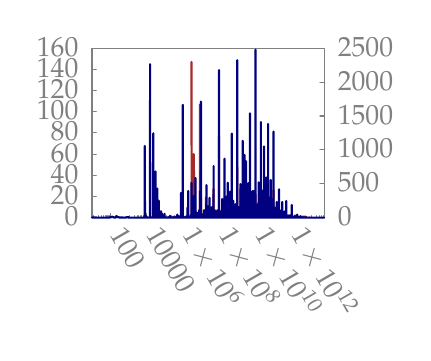
\begin{tikzpicture}[gnuplot, scale=0.3]
%% generated with GNUPLOT 5.2p2 (Lua 5.3; terminal rev. 99, script rev. 102)
%% wo 11 jul 2018 11:38:44 CEST
\path (0.000,0.000) rectangle (12.500,8.750);
\gpcolor{rgb color={0.502,0.502,0.502}}
\gpsetlinetype{gp lt border}
\gpsetdashtype{gp dt solid}
\gpsetlinewidth{1.00}
\draw[gp path] (1.012,1.264)--(1.192,1.264);
\node[gp node right] at (0.828,1.264) {$0$};
\draw[gp path] (1.012,2.161)--(1.192,2.161);
\node[gp node right] at (0.828,2.161) {$20$};
\draw[gp path] (1.012,3.058)--(1.192,3.058);
\node[gp node right] at (0.828,3.058) {$40$};
\draw[gp path] (1.012,3.955)--(1.192,3.955);
\node[gp node right] at (0.828,3.955) {$60$};
\draw[gp path] (1.012,4.853)--(1.192,4.853);
\node[gp node right] at (0.828,4.853) {$80$};
\draw[gp path] (1.012,5.750)--(1.192,5.750);
\node[gp node right] at (0.828,5.750) {$100$};
\draw[gp path] (1.012,6.647)--(1.192,6.647);
\node[gp node right] at (0.828,6.647) {$120$};
\draw[gp path] (1.012,7.544)--(1.192,7.544);
\node[gp node right] at (0.828,7.544) {$140$};
\draw[gp path] (1.012,8.441)--(1.192,8.441);
\node[gp node right] at (0.828,8.441) {$160$};
\draw[gp path] (1.073,1.264)--(1.073,1.354);
\draw[gp path] (1.290,1.264)--(1.290,1.354);
\draw[gp path] (1.421,1.264)--(1.421,1.354);
\draw[gp path] (1.514,1.264)--(1.514,1.354);
\draw[gp path] (1.587,1.264)--(1.587,1.354);
\draw[gp path] (1.647,1.264)--(1.647,1.354);
\draw[gp path] (1.698,1.264)--(1.698,1.354);
\draw[gp path] (1.742,1.264)--(1.742,1.354);
\draw[gp path] (1.781,1.264)--(1.781,1.444);
\node[gp node left,rotate=-60] at (1.781,1.080) {$100$};
\draw[gp path] (2.610,1.264)--(2.610,1.354);
\draw[gp path] (2.827,1.264)--(2.827,1.354);
\draw[gp path] (2.958,1.264)--(2.958,1.354);
\draw[gp path] (3.052,1.264)--(3.052,1.354);
\draw[gp path] (3.125,1.264)--(3.125,1.354);
\draw[gp path] (3.184,1.264)--(3.184,1.354);
\draw[gp path] (3.235,1.264)--(3.235,1.354);
\draw[gp path] (3.279,1.264)--(3.279,1.354);
\draw[gp path] (3.318,1.264)--(3.318,1.444);
\node[gp node left,rotate=-60] at (3.318,1.080) {$10000$};
\draw[gp path] (4.148,1.264)--(4.148,1.354);
\draw[gp path] (4.365,1.264)--(4.365,1.354);
\draw[gp path] (4.495,1.264)--(4.495,1.354);
\draw[gp path] (4.589,1.264)--(4.589,1.354);
\draw[gp path] (4.662,1.264)--(4.662,1.354);
\draw[gp path] (4.722,1.264)--(4.722,1.354);
\draw[gp path] (4.773,1.264)--(4.773,1.354);
\draw[gp path] (4.817,1.264)--(4.817,1.354);
\draw[gp path] (4.856,1.264)--(4.856,1.444);
\node[gp node left,rotate=-60] at (4.856,1.080) {$1\times10^{6}$};
\draw[gp path] (5.685,1.264)--(5.685,1.354);
\draw[gp path] (5.902,1.264)--(5.902,1.354);
\draw[gp path] (6.033,1.264)--(6.033,1.354);
\draw[gp path] (6.126,1.264)--(6.126,1.354);
\draw[gp path] (6.199,1.264)--(6.199,1.354);
\draw[gp path] (6.259,1.264)--(6.259,1.354);
\draw[gp path] (6.310,1.264)--(6.310,1.354);
\draw[gp path] (6.354,1.264)--(6.354,1.354);
\draw[gp path] (6.393,1.264)--(6.393,1.444);
\node[gp node left,rotate=-60] at (6.393,1.080) {$1\times10^{8}$};
\draw[gp path] (7.223,1.264)--(7.223,1.354);
\draw[gp path] (7.440,1.264)--(7.440,1.354);
\draw[gp path] (7.570,1.264)--(7.570,1.354);
\draw[gp path] (7.664,1.264)--(7.664,1.354);
\draw[gp path] (7.737,1.264)--(7.737,1.354);
\draw[gp path] (7.797,1.264)--(7.797,1.354);
\draw[gp path] (7.847,1.264)--(7.847,1.354);
\draw[gp path] (7.891,1.264)--(7.891,1.354);
\draw[gp path] (7.930,1.264)--(7.930,1.444);
\node[gp node left,rotate=-60] at (7.930,1.080) {$1\times10^{10}$};
\draw[gp path] (8.760,1.264)--(8.760,1.354);
\draw[gp path] (8.977,1.264)--(8.977,1.354);
\draw[gp path] (9.108,1.264)--(9.108,1.354);
\draw[gp path] (9.201,1.264)--(9.201,1.354);
\draw[gp path] (9.274,1.264)--(9.274,1.354);
\draw[gp path] (9.334,1.264)--(9.334,1.354);
\draw[gp path] (9.385,1.264)--(9.385,1.354);
\draw[gp path] (9.429,1.264)--(9.429,1.354);
\draw[gp path] (9.468,1.264)--(9.468,1.444);
\node[gp node left,rotate=-60] at (9.468,1.080) {$1\times10^{12}$};
\draw[gp path] (10.297,1.264)--(10.297,1.354);
\draw[gp path] (10.515,1.264)--(10.515,1.354);
\draw[gp path] (10.645,1.264)--(10.645,1.354);
\draw[gp path] (10.739,1.264)--(10.739,1.354);
\draw[gp path] (10.812,1.264)--(10.812,1.354);
\draw[gp path] (10.843,1.264)--(10.663,1.264);
\node[gp node left] at (11.027,1.264) {$0$};
\draw[gp path] (10.843,2.699)--(10.663,2.699);
\node[gp node left] at (11.027,2.699) {$500$};
\draw[gp path] (10.843,4.135)--(10.663,4.135);
\node[gp node left] at (11.027,4.135) {$1000$};
\draw[gp path] (10.843,5.570)--(10.663,5.570);
\node[gp node left] at (11.027,5.570) {$1500$};
\draw[gp path] (10.843,7.006)--(10.663,7.006);
\node[gp node left] at (11.027,7.006) {$2000$};
\draw[gp path] (10.843,8.441)--(10.663,8.441);
\node[gp node left] at (11.027,8.441) {$2500$};
\draw[gp path] (1.012,8.441)--(1.012,1.264)--(10.843,1.264)--(10.843,8.441)--cycle;
\gpcolor{rgb color={0.647,0.165,0.165}}
\gpsetlinewidth{2.00}
\draw[gp path] (5.222,7.858)--(5.236,1.309)--(5.254,1.309)--(5.282,1.309)--(5.302,1.309)%
  --(5.314,1.309)--(5.318,1.354)--(5.318,3.955)--(5.350,1.309)--(5.380,1.309)--(5.393,1.533)%
  --(5.424,1.309)--(5.454,1.354)--(5.496,1.309)--(5.505,1.309)--(5.505,1.354)--(5.535,1.309)%
  --(5.541,1.309)--(5.542,1.309)--(5.549,1.354)--(5.550,1.399)--(5.554,1.309)--(5.569,1.309)%
  --(5.570,1.309)--(5.582,1.309)--(5.589,1.443)--(5.589,1.309)--(5.589,6.064)--(5.624,1.937)%
  --(5.641,1.309)--(5.652,1.309)--(5.656,1.354)--(5.659,1.309)--(5.679,1.309)--(5.683,1.309)%
  --(5.684,1.309)--(5.685,1.354)--(5.697,1.309)--(5.712,1.354)--(5.734,1.309)--(5.735,1.309)%
  --(5.736,1.354)--(5.737,1.354)--(5.759,1.309)--(5.760,1.354)--(5.781,1.399)--(5.786,1.309)%
  --(5.801,1.354)--(5.820,1.488)--(5.820,1.309)--(5.820,1.354)--(5.834,1.309)--(5.838,1.399)%
  --(5.839,2.116)--(5.840,1.309)--(5.852,1.309)--(5.855,1.443)--(5.856,1.488)--(5.860,1.309)%
  --(5.872,1.309)--(5.872,1.399)--(5.887,1.309)--(5.887,1.354)--(5.911,1.309)--(5.913,1.309)%
  --(5.916,1.399)--(5.917,1.713)--(5.923,1.309)--(5.930,1.309)--(5.930,1.354)--(5.933,1.309)%
  --(5.943,1.443)--(5.943,1.309)--(5.956,1.309)--(5.968,1.309)--(5.977,1.309)--(5.979,1.623)%
  --(5.980,1.623)--(5.987,1.309)--(5.989,1.309)--(5.991,1.309)--(5.991,1.399)--(5.999,1.309)%
  --(6.001,1.309)--(6.002,1.309)--(6.012,1.309)--(6.012,1.354)--(6.013,1.443)--(6.023,1.354)%
  --(6.025,1.309)--(6.032,1.309)--(6.032,1.443)--(6.033,1.399)--(6.040,1.309)--(6.042,1.488)%
  --(6.042,1.309)--(6.045,1.309)--(6.050,1.309)--(6.051,1.309)--(6.052,1.399)--(6.060,1.309)%
  --(6.061,1.488)--(6.061,1.309)--(6.070,1.399)--(6.070,1.443)--(6.078,1.578)--(6.079,1.309)%
  --(6.080,1.309)--(6.087,1.354)--(6.093,1.309)--(6.095,1.399)--(6.095,1.354)--(6.103,1.488)%
  --(6.103,1.309)--(6.111,1.309)--(6.111,1.399)--(6.111,1.309)--(6.119,1.443)--(6.119,1.399)%
  --(6.126,1.309)--(6.126,1.443)--(6.126,1.354)--(6.133,1.309)--(6.133,1.354)--(6.134,1.309)%
  --(6.139,1.309)--(6.141,1.354)--(6.141,1.309)--(6.148,1.488)--(6.148,1.399)--(6.154,1.309)%
  --(6.154,1.578)--(6.155,2.475)--(6.158,1.309)--(6.160,1.309)--(6.161,1.399)--(6.162,1.578)%
  --(6.162,1.309)--(6.168,1.399)--(6.168,1.354)--(6.171,1.309)--(6.174,1.309)--(6.174,1.354)%
  --(6.175,1.309)--(6.181,1.309)--(6.182,1.309)--(6.184,1.309)--(6.185,1.309)--(6.186,1.309)%
  --(6.187,1.533)--(6.187,1.399)--(6.188,1.309)--(6.193,1.354)--(6.199,1.309)--(6.199,1.443)%
  --(6.199,1.399)--(6.205,1.309)--(6.205,1.488)--(6.205,1.309)--(6.210,1.309)--(6.211,1.354)%
  --(6.211,1.309)--(6.211,1.354)--(6.212,1.309)--(6.213,1.309)--(6.215,1.309)--(6.216,1.578)%
  --(6.217,1.309)--(6.217,1.399)--(6.220,1.309)--(6.222,1.533)--(6.222,1.309)--(6.223,1.309)%
  --(6.227,1.309)--(6.228,1.309)--(6.228,1.354)--(6.228,1.309)--(6.229,1.309)--(6.230,1.309)%
  --(6.232,1.309)--(6.233,1.354)--(6.233,1.309)--(6.234,1.309)--(6.238,1.309)--(6.238,1.354)%
  --(6.242,1.309)--(6.244,1.354)--(6.244,1.533)--(6.245,1.309)--(6.249,1.488)--(6.249,1.354)%
  --(6.252,1.309)--(6.254,1.354)--(6.254,1.309)--(6.254,1.354)--(6.255,1.309)--(6.259,1.354)%
  --(6.264,1.309)--(6.264,1.354)--(6.265,1.309)--(6.269,1.309)--(6.274,1.309)--(6.276,1.309)%
  --(6.278,1.443)--(6.283,1.354)--(6.288,1.533)--(6.288,1.309)--(6.289,1.309)--(6.292,1.309)%
  --(6.292,1.488)--(6.292,1.309)--(6.296,1.309)--(6.297,1.309)--(6.297,1.354)--(6.300,1.309)%
  --(6.301,1.354)--(6.305,1.488)--(6.306,1.354)--(6.307,1.309)--(6.309,1.309)--(6.310,1.309)%
  --(6.310,1.354)--(6.314,1.309)--(6.314,1.578)--(6.314,1.309)--(6.318,1.309)--(6.318,1.533)%
  --(6.322,1.488)--(6.323,1.309)--(6.325,1.309)--(6.326,1.399)--(6.327,1.399)--(6.330,1.309)%
  --(6.331,1.309)--(6.334,1.309)--(6.334,1.488)--(6.334,1.309)--(6.335,1.309)--(6.336,1.309)%
  --(6.338,1.443)--(6.341,1.309)--(6.342,1.354)--(6.343,1.309)--(6.346,1.399)--(6.346,1.309)%
  --(6.350,1.309)--(6.350,1.399)--(6.352,1.309)--(6.354,1.533)--(6.354,1.309)--(6.356,1.309)%
  --(6.357,1.309)--(6.357,1.443)--(6.358,1.309)--(6.361,1.354)--(6.364,1.309)--(6.365,1.354)%
  --(6.368,1.354)--(6.369,1.309)--(6.372,1.354)--(6.376,1.309)--(6.379,1.309)--(6.379,1.443)%
  --(6.379,1.309)--(6.382,1.354)--(6.383,1.354)--(6.384,1.309)--(6.386,1.309)--(6.386,1.399)%
  --(6.386,1.309)--(6.386,1.354)--(6.386,1.309)--(6.389,2.161)--(6.390,4.718)--(6.391,1.309)%
  --(6.392,1.309)--(6.393,1.309)--(6.393,1.623)--(6.393,1.309)--(6.393,2.296)--(6.393,1.309)%
  --(6.395,1.309)--(6.396,1.309)--(6.396,1.623)--(6.396,1.354)--(6.398,1.309)--(6.399,1.443)%
  --(6.400,1.309)--(6.401,1.309)--(6.402,1.309)--(6.403,1.443)--(6.406,1.533)--(6.406,1.488)%
  --(6.409,1.354)--(6.411,1.309)--(6.412,1.309)--(6.416,1.309)--(6.417,1.309)--(6.418,1.399)%
  --(6.421,1.309)--(6.421,1.354)--(6.422,1.399)--(6.424,1.399)--(6.425,1.309)--(6.427,1.488)%
  --(6.430,1.354)--(6.431,1.354)--(6.433,1.309)--(6.434,1.309)--(6.434,1.354)--(6.436,1.309)%
  --(6.437,1.354)--(6.438,1.309)--(6.440,1.399)--(6.440,1.309)--(6.442,1.309)--(6.445,1.309)%
  --(6.445,1.354)--(6.448,1.399)--(6.451,1.354)--(6.451,1.309)--(6.453,1.309)--(6.454,1.354)%
  --(6.456,1.309)--(6.456,1.354)--(6.457,1.354)--(6.459,1.354)--(6.461,1.309)--(6.462,1.309)%
  --(6.462,1.354)--(6.462,1.309)--(6.464,1.399)--(6.466,1.309)--(6.467,1.309)--(6.469,1.309)%
  --(6.470,1.309)--(6.472,1.354)--(6.473,1.309)--(6.475,1.309)--(6.478,1.309)--(6.478,1.354)%
  --(6.480,1.443)--(6.481,1.309)--(6.482,1.309)--(6.483,1.309)--(6.483,1.399)--(6.485,1.309)%
  --(6.485,1.354)--(6.486,1.309)--(6.488,1.309)--(6.490,1.309)--(6.490,1.399)--(6.491,1.309)%
  --(6.492,1.309)--(6.493,1.399)--(6.493,1.309)--(6.495,1.309)--(6.495,1.399)--(6.496,1.309)%
  --(6.498,1.309)--(6.498,1.399)--(6.500,1.399)--(6.501,1.309)--(6.503,1.399)--(6.504,1.309)%
  --(6.505,1.309)--(6.505,1.399)--(6.507,1.354)--(6.510,1.488)--(6.512,1.354)--(6.514,1.399)%
  --(6.515,1.309)--(6.519,1.354)--(6.521,1.399)--(6.522,1.309)--(6.524,1.309)--(6.524,1.399)%
  --(6.524,1.309)--(6.526,1.488)--(6.526,1.533)--(6.528,1.309)--(6.528,1.443)--(6.531,1.309)%
  --(6.532,1.309)--(6.532,1.443)--(6.535,1.354)--(6.535,1.309)--(6.536,1.309)--(6.537,1.488)%
  --(6.537,1.309)--(6.539,1.309)--(6.541,1.309)--(6.543,1.399)--(6.544,1.354)--(6.545,1.309)%
  --(6.546,1.309)--(6.547,1.309)--(6.547,1.533)--(6.548,1.309)--(6.550,1.309)--(6.552,1.309)%
  --(6.554,1.354)--(6.556,1.309)--(6.556,1.354)--(6.556,1.309)--(6.558,1.309)--(6.558,1.354)%
  --(6.559,1.309)--(6.560,1.399)--(6.560,1.354)--(6.562,1.309)--(6.563,1.309)--(6.564,1.309)%
  --(6.564,1.354)--(6.564,1.309)--(6.566,1.309)--(6.566,1.354)--(6.568,1.399)--(6.570,1.354)%
  --(6.571,1.309)--(6.572,1.354)--(6.577,1.309)--(6.578,1.354)--(6.578,1.309)--(6.579,1.399)%
  --(6.581,1.309)--(6.581,1.354)--(6.583,1.354)--(6.585,1.309)--(6.585,1.354)--(6.587,1.578)%
  --(6.587,1.399)--(6.588,1.309)--(6.589,1.309)--(6.590,1.309)--(6.591,1.354)--(6.591,1.309)%
  --(6.593,1.309)--(6.595,1.309)--(6.596,1.309)--(6.596,1.399)--(6.596,1.309)--(6.598,1.309)%
  --(6.600,1.309)--(6.602,1.309)--(6.604,1.309)--(6.605,1.309)--(6.606,1.309)--(6.607,1.399)%
  --(6.607,1.354)--(6.609,1.309)--(6.609,1.443)--(6.609,1.309)--(6.610,1.309)--(6.612,1.399)%
  --(6.612,1.309)--(6.613,1.309)--(6.614,1.309)--(6.617,1.309)--(6.619,1.354)--(6.619,1.309)%
  --(6.621,1.488)--(6.622,1.309)--(6.622,1.847)--(6.623,1.982)--(6.624,1.399)--(6.624,1.713)%
  --(6.626,1.309)--(6.626,1.354)--(6.627,1.354)--(6.629,1.309)--(6.631,1.443)--(6.631,1.309)%
  --(6.632,1.309)--(6.633,1.309)--(6.634,1.309)--(6.636,1.309)--(6.637,1.309)--(6.639,1.309)%
  --(6.642,1.354)--(6.642,1.309)--(6.643,1.309)--(6.643,1.399)--(6.645,1.354)--(6.645,1.309)%
  --(6.647,1.309)--(6.648,1.309)--(6.648,1.399)--(6.650,1.399)--(6.651,1.399)--(6.652,1.309)%
  --(6.653,1.309)--(6.653,1.354)--(6.654,1.309)--(6.654,1.443)--(6.655,1.309)--(6.656,1.309)%
  --(6.656,1.354)--(6.657,1.488)--(6.657,1.309)--(6.658,1.309)--(6.659,1.399)--(6.660,1.354)%
  --(6.660,1.309)--(6.662,1.309)--(6.662,1.399)--(6.663,1.309)--(6.663,1.354)--(6.665,1.354)%
  --(6.665,1.309)--(6.666,1.354)--(6.668,1.309)--(6.669,1.309)--(6.669,1.354)--(6.670,1.354)%
  --(6.671,1.443)--(6.671,1.309)--(6.672,1.488)--(6.672,1.309)--(6.674,1.354)--(6.676,1.399)%
  --(6.678,1.354)--(6.679,1.309)--(6.681,1.488)--(6.682,1.488)--(6.684,1.354)--(6.685,1.309)%
  --(6.685,1.354)--(6.685,1.309)--(6.686,1.309)--(6.687,1.309)--(6.688,1.309)--(6.689,1.309)%
  --(6.689,1.354)--(6.690,1.309)--(6.691,1.354)--(6.692,1.309)--(6.692,1.354)--(6.693,1.309)%
  --(6.694,1.309)--(6.695,1.309)--(6.696,1.309)--(6.697,1.399)--(6.698,1.623)--(6.698,1.309)%
  --(6.699,1.399)--(6.699,1.488)--(6.700,1.309)--(6.700,1.354)--(6.701,1.309)--(6.702,1.309)%
  --(6.703,1.354)--(6.704,1.399)--(6.704,1.309)--(6.705,1.354)--(6.706,1.309)--(6.706,1.354)%
  --(6.707,1.309)--(6.708,1.354)--(6.709,1.309)--(6.710,1.309)--(6.711,1.354)--(6.712,1.309)%
  --(6.713,1.354)--(6.714,1.309)--(6.714,1.443)--(6.715,1.443)--(6.717,1.488)--(6.718,1.309)%
  --(6.719,1.309)--(6.720,1.309)--(6.721,1.354)--(6.721,1.309)--(6.722,1.443)--(6.723,1.443)%
  --(6.723,1.399)--(6.724,1.309)--(6.724,1.399)--(6.727,1.354)--(6.728,1.309)--(6.729,1.399)%
  --(6.730,1.309)--(6.733,1.309)--(6.734,1.309)--(6.735,1.354)--(6.736,1.354)--(6.736,1.443)%
  --(6.737,1.309)--(6.738,1.309)--(6.739,1.309)--(6.741,1.354)--(6.742,1.309)--(6.743,1.309)%
  --(6.745,1.309)--(6.746,1.354)--(6.746,1.309)--(6.747,1.309)--(6.747,1.354)--(6.748,1.309)%
  --(6.748,1.399)--(6.748,1.309)--(6.749,1.309)--(6.750,1.354)--(6.750,1.309)--(6.751,1.309)%
  --(6.752,1.354)--(6.753,1.309)--(6.754,1.309)--(6.755,1.309)--(6.756,1.399)--(6.757,1.309)%
  --(6.757,1.354)--(6.758,1.668)--(6.759,1.713)--(6.759,1.309)--(6.760,1.623)--(6.761,1.309)%
  --(6.762,1.354)--(6.762,1.309)--(6.763,1.354)--(6.763,1.309)--(6.764,1.309)--(6.765,1.309)%
  --(6.766,1.309)--(6.767,1.354)--(6.767,1.309)--(6.768,1.309)--(6.769,1.309)--(6.769,1.354)%
  --(6.769,1.309)--(6.770,1.309)--(6.770,1.354)--(6.771,1.309)--(6.773,1.309)--(6.774,1.309)%
  --(6.776,1.309)--(6.778,1.354)--(6.779,1.354)--(6.779,1.309)--(6.780,1.354)--(6.780,1.399)%
  --(6.781,1.309)--(6.782,1.399)--(6.782,1.309)--(6.784,1.309)--(6.784,1.354)--(6.785,1.309)%
  --(6.785,1.399)--(6.785,1.309)--(6.786,1.354)--(6.787,1.309)--(6.787,1.399)--(6.788,1.354)%
  --(6.789,1.309)--(6.790,1.354)--(6.791,1.309)--(6.791,1.399)--(6.792,1.354)--(6.792,1.309)%
  --(6.793,1.309)--(6.794,1.354)--(6.795,1.309)--(6.796,1.354)--(6.797,1.309)--(6.797,1.399)%
  --(6.798,1.309)--(6.798,1.399)--(6.799,1.309)--(6.800,1.309)--(6.800,1.354)--(6.801,1.309)%
  --(6.802,1.399)--(6.803,1.309)--(6.803,1.354)--(6.804,1.309)--(6.804,1.354)--(6.805,1.309)%
  --(6.806,1.354)--(6.807,1.309)--(6.807,1.443)--(6.807,1.354)--(6.807,1.309)--(6.808,1.354)%
  --(6.809,1.354)--(6.810,1.443)--(6.810,1.354)--(6.811,1.309)--(6.812,1.443)--(6.813,1.309)%
  --(6.814,1.309)--(6.815,1.309)--(6.816,1.309)--(6.817,1.399)--(6.817,1.309)--(6.818,1.354)%
  --(6.820,1.309)--(6.821,1.309)--(6.822,1.309)--(6.822,1.399)--(6.823,1.309)--(6.824,1.309)%
  --(6.825,1.488)--(6.826,1.309)--(6.827,1.354)--(6.827,1.309)--(6.828,1.309)--(6.829,1.309)%
  --(6.829,1.354)--(6.830,1.354)--(6.830,1.309)--(6.831,1.309)--(6.832,1.309)--(6.833,1.309)%
  --(6.834,1.309)--(6.834,1.354)--(6.835,1.399)--(6.836,1.354)--(6.837,1.354)--(6.837,1.309)%
  --(6.838,1.309)--(6.838,1.354)--(6.838,1.309)--(6.839,1.309)--(6.840,1.309)--(6.840,1.354)%
  --(6.841,1.309)--(6.842,1.309)--(6.843,1.309)--(6.844,1.354)--(6.844,1.309)--(6.846,1.309)%
  --(6.847,1.354)--(6.848,1.309)--(6.849,1.309)--(6.850,1.354)--(6.850,1.309)--(6.851,1.309)%
  --(6.851,1.443)--(6.852,1.309)--(6.853,1.399)--(6.854,1.309)--(6.855,1.443)--(6.855,1.309)%
  --(6.855,1.623)--(6.855,1.354)--(6.856,1.623)--(6.857,1.399)--(6.857,1.309)--(6.858,1.309)%
  --(6.859,1.309)--(6.860,1.309)--(6.861,1.309)--(6.862,1.309)--(6.862,1.399)--(6.863,1.309)%
  --(6.863,1.354)--(6.863,1.309)--(6.863,1.399)--(6.864,1.309)--(6.864,1.354)--(6.865,1.309)%
  --(6.865,1.354)--(6.866,1.443)--(6.866,1.309)--(6.867,1.309)--(6.868,1.309)--(6.869,1.354)%
  --(6.869,1.309)--(6.870,1.309)--(6.870,1.354)--(6.871,1.309)--(6.872,1.309)--(6.873,1.309)%
  --(6.874,1.354)--(6.875,1.309)--(6.876,1.354)--(6.877,1.309)--(6.878,1.399)--(6.879,1.309)%
  --(6.880,1.354)--(6.881,1.354)--(6.881,1.309)--(6.883,1.309)--(6.883,1.354)--(6.884,1.309)%
  --(6.885,1.354)--(6.886,1.309)--(6.887,1.309)--(6.889,1.354)--(6.891,1.309)--(6.892,1.354)%
  --(6.892,1.309)--(6.893,1.309)--(6.894,1.399)--(6.895,1.309)--(6.896,1.354)--(6.896,1.309)%
  --(6.897,1.309)--(6.898,1.309)--(6.898,1.354)--(6.899,1.309)--(6.900,1.309)--(6.901,1.309)%
  --(6.901,1.354)--(6.902,1.309)--(6.903,1.309)--(6.904,1.309)--(6.905,1.309)--(6.907,1.309)%
  --(6.910,1.354)--(6.910,1.309)--(6.911,1.309)--(6.912,1.354)--(6.912,1.309)--(6.913,1.309)%
  --(6.914,1.399)--(6.915,1.309)--(6.916,1.309)--(6.917,1.309)--(6.917,1.354)--(6.917,1.309)%
  --(6.918,1.309)--(6.919,1.309)--(6.920,1.309)--(6.920,1.354)--(6.921,1.309)--(6.923,1.309)%
  --(6.923,1.443)--(6.924,1.354)--(6.924,1.309)--(6.925,1.309)--(6.926,1.309)--(6.926,1.354)%
  --(6.926,1.309)--(6.927,1.309)--(6.927,1.354)--(6.927,1.309)--(6.928,1.309)--(6.929,1.309)%
  --(6.929,1.354)--(6.929,2.071)--(6.930,1.309)--(6.930,2.206)--(6.930,1.309)--(6.930,1.757)%
  --(6.930,1.309)--(6.931,1.399)--(6.931,1.309)--(6.931,1.354)--(6.931,1.443)--(6.931,1.309)%
  --(6.932,1.309)--(6.933,1.354)--(6.933,1.309)--(6.933,1.443)--(6.934,1.309)--(6.935,1.309)%
  --(6.936,1.354)--(6.936,1.399)--(6.937,1.309)--(6.938,1.309)--(6.940,1.309)--(6.941,1.309)%
  --(6.941,1.354)--(6.941,1.309)--(6.942,1.309)--(6.943,1.309)--(6.943,1.399)--(6.943,1.309)%
  --(6.944,1.309)--(6.945,1.354)--(6.946,1.309)--(6.947,1.309)--(6.947,1.354)--(6.948,1.309)%
  --(6.948,1.354)--(6.949,1.399)--(6.950,1.309)--(6.951,1.354)--(6.952,1.309)--(6.953,1.309)%
  --(6.954,1.309)--(6.954,1.354)--(6.955,1.309)--(6.957,1.309)--(6.958,1.309)--(6.959,1.309)%
  --(6.960,1.354)--(6.960,1.309)--(6.961,1.354)--(6.961,1.399)--(6.962,1.309)--(6.963,1.309)%
  --(6.964,1.309)--(6.965,1.309)--(6.966,1.354)--(6.966,1.309)--(6.967,1.309)--(6.968,1.309)%
  --(6.969,1.309)--(6.970,1.309)--(6.971,1.309)--(6.971,1.354)--(6.972,1.309)--(6.973,1.309)%
  --(6.974,1.309)--(6.975,1.399)--(6.975,1.309)--(6.977,1.309)--(6.978,1.309)--(6.979,1.309)%
  --(6.980,1.399)--(6.980,1.309)--(6.981,1.309)--(6.981,1.354)--(6.982,1.309)--(6.982,1.354)%
  --(6.984,1.309)--(6.985,1.309)--(6.986,1.309)--(6.987,1.309)--(6.988,1.309)--(6.989,1.309)%
  --(6.990,1.488)--(6.991,1.488)--(6.991,1.309)--(6.991,1.354)--(6.992,1.309)--(6.993,1.309)%
  --(6.994,1.309)--(6.995,1.309)--(6.996,1.309)--(6.997,1.309)--(6.998,1.309)--(6.999,1.354)%
  --(7.000,1.309)--(7.001,1.354)--(7.001,1.309)--(7.002,1.309)--(7.003,1.309)--(7.004,1.309)%
  --(7.005,1.309)--(7.006,1.309)--(7.007,1.309)--(7.008,1.309)--(7.009,1.354)--(7.009,1.309)%
  --(7.010,1.309)--(7.011,1.309)--(7.012,1.309)--(7.013,1.309)--(7.014,1.309)--(7.015,1.309)%
  --(7.017,1.309)--(7.017,1.443)--(7.017,1.309)--(7.018,1.309)--(7.018,1.354)--(7.018,1.309)%
  --(7.019,1.309)--(7.019,1.354)--(7.020,1.354)--(7.020,1.309)--(7.021,1.309)--(7.022,1.309)%
  --(7.024,1.309)--(7.025,1.309)--(7.027,1.309)--(7.028,1.309)--(7.029,1.309)--(7.030,1.309)%
  --(7.032,1.309)--(7.034,1.309)--(7.035,1.309)--(7.035,1.354)--(7.036,1.399)--(7.037,1.354)%
  --(7.037,1.309)--(7.040,1.309)--(7.041,1.309)--(7.042,1.354)--(7.042,1.309)--(7.043,1.399)%
  --(7.043,1.354)--(7.043,1.309)--(7.044,1.309)--(7.044,1.354)--(7.044,1.309)--(7.046,1.309)%
  --(7.047,1.309)--(7.048,1.309)--(7.049,1.309)--(7.050,1.309)--(7.052,1.309)--(7.053,1.309)%
  --(7.054,1.309)--(7.054,1.354)--(7.055,1.309)--(7.056,1.309)--(7.057,1.309)--(7.058,1.354)%
  --(7.058,1.309)--(7.059,1.354)--(7.059,1.309)--(7.060,1.309)--(7.060,1.354)--(7.061,1.309)%
  --(7.062,1.309)--(7.064,1.354)--(7.065,1.354)--(7.066,1.399)--(7.066,1.354)--(7.067,1.309)%
  --(7.068,1.309)--(7.069,1.354)--(7.069,1.309)--(7.069,1.354)--(7.070,1.309)--(7.071,1.309)%
  --(7.071,1.354)--(7.071,1.309)--(7.072,1.309)--(7.073,1.309)--(7.074,1.309)--(7.074,1.399)%
  --(7.075,1.309)--(7.076,1.309)--(7.077,1.309)--(7.077,1.354)--(7.077,1.309)--(7.078,1.309)%
  --(7.079,1.309)--(7.080,1.309)--(7.081,1.399)--(7.081,1.354)--(7.082,1.443)--(7.083,1.309)%
  --(7.084,1.309)--(7.085,1.354)--(7.085,1.309)--(7.085,1.354)--(7.086,1.309)--(7.086,1.354)%
  --(7.087,1.309)--(7.087,1.399)--(7.087,1.354)--(7.087,1.309)--(7.088,1.309)--(7.089,1.309)%
  --(7.090,1.309)--(7.091,1.309)--(7.091,1.354)--(7.092,1.309)--(7.093,1.309)--(7.094,1.309)%
  --(7.094,1.354)--(7.095,1.309)--(7.096,1.309)--(7.096,1.354)--(7.096,1.309)--(7.098,1.309)%
  --(7.099,1.309)--(7.101,1.309)--(7.102,1.309)--(7.103,1.309)--(7.104,1.354)--(7.104,1.309)%
  --(7.105,1.309)--(7.106,1.354)--(7.107,1.399)--(7.107,1.309)--(7.108,1.309)--(7.109,1.309)%
  --(7.110,1.354)--(7.110,1.309)--(7.110,1.354)--(7.110,1.399)--(7.111,1.309)--(7.111,1.354)%
  --(7.111,1.309)--(7.113,1.309)--(7.114,1.309)--(7.115,1.309)--(7.117,1.309)--(7.118,1.309)%
  --(7.119,1.309)--(7.121,1.309)--(7.122,1.309)--(7.123,1.309)--(7.124,1.309)--(7.125,1.309)%
  --(7.126,1.309)--(7.126,1.443)--(7.126,1.309)--(7.127,1.354)--(7.127,1.399)--(7.128,1.399)%
  --(7.128,1.309)--(7.129,1.309)--(7.130,1.309)--(7.131,1.309)--(7.132,1.309)--(7.133,1.309)%
  --(7.134,1.309)--(7.136,1.309)--(7.137,1.309)--(7.138,1.309)--(7.139,1.309)--(7.140,1.309)%
  --(7.141,1.309)--(7.142,1.309)--(7.143,1.309)--(7.144,1.309)--(7.145,1.309)--(7.146,1.309)%
  --(7.147,1.309)--(7.148,1.354)--(7.148,1.309)--(7.149,1.309)--(7.149,1.399)--(7.149,1.309)%
  --(7.150,1.309)--(7.150,1.399)--(7.150,1.309)--(7.151,1.309)--(7.152,1.309)--(7.153,1.309)%
  --(7.154,1.309)--(7.155,1.309)--(7.156,1.309)--(7.157,1.309)--(7.158,1.309)--(7.158,1.354)%
  --(7.158,1.309)--(7.159,1.309)--(7.160,1.354)--(7.160,1.309)--(7.161,2.071)--(7.161,1.309)%
  --(7.161,1.354)--(7.161,3.417)--(7.161,1.309)--(7.162,1.309)--(7.162,2.296)--(7.162,1.309)%
  --(7.162,1.354)--(7.162,1.309)--(7.162,1.354)--(7.162,1.309)--(7.163,1.309)--(7.163,1.399)%
  --(7.163,1.309)--(7.164,1.309)--(7.165,1.354)--(7.165,1.443)--(7.165,1.354)--(7.165,1.309)%
  --(7.166,1.309)--(7.167,1.309)--(7.168,1.354)--(7.169,1.354)--(7.169,1.309)--(7.170,1.354)%
  --(7.170,1.309)--(7.171,1.309)--(7.172,1.309)--(7.173,1.309)--(7.174,1.309)--(7.174,1.354)%
  --(7.174,1.309)--(7.175,1.309)--(7.176,1.309)--(7.177,1.309)--(7.178,1.309)--(7.179,1.309)%
  --(7.180,1.309)--(7.181,1.309)--(7.182,1.309)--(7.183,1.354)--(7.184,1.309)--(7.184,1.354)%
  --(7.184,1.309)--(7.185,1.309)--(7.186,1.309)--(7.187,1.309)--(7.187,1.399)--(7.188,1.309)%
  --(7.188,1.354)--(7.189,1.309)--(7.190,1.354)--(7.190,1.309)--(7.191,1.309)--(7.192,1.309)%
  --(7.193,1.309)--(7.193,1.354)--(7.193,1.309)--(7.194,1.309)--(7.195,1.309)--(7.196,1.309)%
  --(7.196,1.354)--(7.197,1.309)--(7.198,1.309)--(7.199,1.309)--(7.200,1.354)--(7.200,1.309)%
  --(7.201,1.354)--(7.202,1.309)--(7.203,1.309)--(7.204,1.309)--(7.205,1.309)--(7.207,1.309)%
  --(7.208,1.309)--(7.209,1.309)--(7.210,1.309)--(7.210,1.399)--(7.210,1.309)--(7.211,1.309)%
  --(7.212,1.309)--(7.213,1.309)--(7.214,1.309)--(7.216,1.309)--(7.217,1.309)--(7.218,1.309)%
  --(7.219,1.309)--(7.220,1.309)--(7.221,1.309)--(7.222,1.309)--(7.222,1.354)--(7.222,1.399)%
  --(7.222,1.309)--(7.223,1.309)--(7.223,1.354)--(7.223,1.309)--(7.224,1.354)--(7.224,1.309)%
  --(7.225,1.309)--(7.226,1.309)--(7.227,1.309)--(7.228,1.309)--(7.228,1.354)--(7.229,1.309)%
  --(7.231,1.309)--(7.232,1.309)--(7.233,1.309)--(7.234,1.309)--(7.235,1.309)--(7.236,1.309)%
  --(7.237,1.309)--(7.238,1.309)--(7.239,1.309)--(7.240,1.309)--(7.241,1.309)--(7.242,1.309)%
  --(7.243,1.309)--(7.244,1.309)--(7.244,1.354)--(7.244,1.309)--(7.245,1.309)--(7.248,1.309)%
  --(7.249,1.309)--(7.250,1.309)--(7.251,1.309)--(7.251,1.354)--(7.252,1.309)--(7.253,1.309)%
  --(7.254,1.309)--(7.255,1.309)--(7.256,1.309)--(7.258,1.309)--(7.259,1.309)--(7.260,1.309)%
  --(7.261,1.309)--(7.262,1.309)--(7.263,1.309)--(7.264,1.309)--(7.265,1.309)--(7.266,1.309)%
  --(7.266,1.354)--(7.267,1.309)--(7.268,1.309)--(7.269,1.309)--(7.270,1.309)--(7.271,1.309)%
  --(7.272,1.354)--(7.273,1.309)--(7.274,1.443)--(7.274,1.309)--(7.276,1.309)--(7.277,1.309)%
  --(7.278,1.309)--(7.279,1.354)--(7.279,1.309)--(7.279,1.399)--(7.280,1.354)--(7.281,1.309)%
  --(7.282,1.309)--(7.283,1.309)--(7.284,1.354)--(7.285,1.354)--(7.285,1.309)--(7.286,1.309)%
  --(7.287,1.309)--(7.288,1.309)--(7.289,1.309)--(7.290,1.309)--(7.291,1.309)--(7.292,1.309)%
  --(7.293,1.309)--(7.294,1.309)--(7.295,1.309)--(7.296,1.309)--(7.296,1.354)--(7.296,1.309)%
  --(7.296,1.399)--(7.297,1.309)--(7.297,2.475)--(7.297,1.309)--(7.297,1.533)--(7.297,1.309)%
  --(7.298,1.354)--(7.298,1.309)--(7.299,1.309)--(7.300,1.309)--(7.300,1.354)--(7.300,1.309)%
  --(7.301,1.309)--(7.302,1.309)--(7.303,1.309)--(7.304,1.354)--(7.304,1.309)--(7.305,1.309)%
  --(7.306,1.309)--(7.307,1.309)--(7.309,1.309)--(7.312,1.309)--(7.314,1.309)--(7.315,1.309)%
  --(7.316,1.309)--(7.316,1.354)--(7.316,1.309)--(7.317,1.309)--(7.318,1.309)--(7.318,1.443)%
  --(7.318,1.309)--(7.318,1.354)--(7.319,1.309)--(7.319,1.354)--(7.319,1.309)--(7.320,1.354)%
  --(7.320,1.309)--(7.321,1.309)--(7.322,1.309)--(7.323,1.354)--(7.324,1.309)--(7.325,1.309)%
  --(7.326,1.309)--(7.327,1.309)--(7.328,1.309)--(7.329,1.309)--(7.330,1.309)--(7.330,1.354)%
  --(7.331,1.309)--(7.331,1.354)--(7.331,1.309)--(7.332,1.309)--(7.333,1.309)--(7.334,1.309)%
  --(7.335,1.309)--(7.336,1.309)--(7.337,1.309)--(7.338,1.309)--(7.339,1.309)--(7.339,1.354)%
  --(7.339,1.309)--(7.340,1.309)--(7.340,1.354)--(7.342,1.309)--(7.343,1.309)--(7.343,1.354)%
  --(7.343,1.309)--(7.344,1.309)--(7.345,1.309)--(7.346,1.309)--(7.347,1.309)--(7.348,1.309)%
  --(7.349,1.309)--(7.350,1.309)--(7.351,1.309)--(7.352,1.354)--(7.352,1.309)--(7.353,1.309)%
  --(7.354,1.309)--(7.355,1.309)--(7.356,1.309)--(7.357,1.309)--(7.358,1.309)--(7.359,1.309)%
  --(7.360,1.309)--(7.361,1.309)--(7.362,1.309)--(7.363,1.309)--(7.364,1.309)--(7.365,1.309)%
  --(7.366,1.309)--(7.368,1.309)--(7.369,1.309)--(7.369,1.354)--(7.370,1.354)--(7.371,1.309)%
  --(7.373,1.309)--(7.374,1.309)--(7.375,1.354)--(7.375,1.309)--(7.376,1.354)--(7.376,1.309)%
  --(7.376,1.354)--(7.376,1.309)--(7.377,1.309)--(7.378,1.309)--(7.379,1.309)--(7.380,1.309)%
  --(7.381,1.309)--(7.382,1.309)--(7.383,1.309)--(7.384,1.309)--(7.386,1.309)--(7.387,1.309)%
  --(7.388,1.309)--(7.389,1.309)--(7.390,1.309)--(7.391,1.309)--(7.392,1.309)--(7.393,1.668)%
  --(7.393,1.309)--(7.393,2.161)--(7.393,1.309)--(7.393,1.847)--(7.393,1.354)--(7.393,1.309)%
  --(7.394,1.309)--(7.395,1.354)--(7.395,1.309)--(7.396,1.354)--(7.396,1.309)--(7.397,1.309)%
  --(7.398,1.309)--(7.399,1.309)--(7.400,1.309)--(7.401,1.309)--(7.402,1.309)--(7.402,1.354)%
  --(7.403,1.354)--(7.403,1.309)--(7.405,1.309)--(7.406,1.309)--(7.407,1.309)--(7.408,1.309)%
  --(7.409,1.309)--(7.410,1.309)--(7.411,1.309)--(7.414,1.309)--(7.415,1.309)--(7.416,1.309)%
  --(7.417,1.309)--(7.418,1.309)--(7.419,1.309)--(7.420,1.309)--(7.421,1.309)--(7.422,1.354)%
  --(7.422,1.309)--(7.423,1.309)--(7.423,1.354)--(7.423,1.309)--(7.424,1.309)--(7.424,1.354)%
  --(7.425,1.309)--(7.426,1.309)--(7.427,1.309)--(7.428,1.309)--(7.429,1.309)--(7.431,1.309)%
  --(7.432,1.309)--(7.434,1.309)--(7.435,1.309)--(7.436,1.309)--(7.437,1.309)--(7.438,1.309)%
  --(7.439,1.309)--(7.440,1.309)--(7.443,1.309)--(7.444,1.309)--(7.444,1.354)--(7.444,1.309)%
  --(7.446,1.309)--(7.447,1.309)--(7.448,1.309)--(7.449,1.309)--(7.450,1.309)--(7.451,1.309)%
  --(7.452,1.309)--(7.453,1.309)--(7.455,1.309)--(7.456,1.309)--(7.457,1.309)--(7.459,1.309)%
  --(7.460,1.309)--(7.461,1.309)--(7.462,1.309)--(7.463,1.309)--(7.464,1.309)--(7.465,1.309)%
  --(7.466,1.309)--(7.467,1.354)--(7.467,1.309)--(7.467,2.744)--(7.468,1.309)--(7.468,1.354)%
  --(7.468,1.309)--(7.469,1.309)--(7.470,1.309)--(7.471,1.309)--(7.472,1.309)--(7.473,1.309)%
  --(7.474,1.309)--(7.475,1.309)--(7.476,1.309)--(7.477,1.309)--(7.478,1.309)--(7.479,1.309)%
  --(7.480,1.309)--(7.481,1.309)--(7.483,1.309)--(7.484,1.309)--(7.485,1.309)--(7.487,1.309)%
  --(7.488,1.309)--(7.489,1.309)--(7.490,1.309)--(7.491,1.309)--(7.493,1.309)--(7.493,1.354)%
  --(7.493,1.309)--(7.494,1.309)--(7.495,1.309)--(7.496,1.309)--(7.497,1.309)--(7.499,1.309)%
  --(7.500,1.309)--(7.501,1.309)--(7.502,1.309)--(7.503,1.309)--(7.505,1.309)--(7.506,1.309)%
  --(7.507,1.309)--(7.508,1.309)--(7.508,1.354)--(7.508,1.309)--(7.510,1.309)--(7.510,1.354)%
  --(7.511,1.309)--(7.512,1.309)--(7.513,1.354)--(7.513,1.309)--(7.514,1.309)--(7.515,1.309)%
  --(7.515,1.354)--(7.515,1.309)--(7.516,1.309)--(7.517,1.309)--(7.518,1.309)--(7.519,1.309)%
  --(7.520,1.309)--(7.521,1.309)--(7.521,1.354)--(7.521,1.309)--(7.522,1.309)--(7.523,1.309)%
  --(7.524,1.309)--(7.525,1.309)--(7.526,1.309)--(7.528,1.309)--(7.528,1.443)--(7.528,1.309)%
  --(7.528,1.533)--(7.528,1.309)--(7.528,1.533)--(7.529,1.309)--(7.530,1.309)--(7.531,1.309)%
  --(7.532,1.309)--(7.533,1.309)--(7.534,1.309)--(7.536,1.309)--(7.537,1.309)--(7.537,1.354)%
  --(7.538,1.309)--(7.539,1.309)--(7.540,1.309)--(7.541,1.309)--(7.543,1.309)--(7.544,1.309)%
  --(7.546,1.309)--(7.547,1.309)--(7.548,1.309)--(7.549,1.309)--(7.550,1.309)--(7.551,1.309)%
  --(7.552,1.309)--(7.553,1.309)--(7.554,1.309)--(7.556,1.309)--(7.557,1.309)--(7.558,1.309)%
  --(7.559,1.309)--(7.560,1.309)--(7.561,1.309)--(7.562,1.309)--(7.563,1.309)--(7.564,1.309)%
  --(7.565,1.309)--(7.566,1.309)--(7.568,1.309)--(7.569,1.309)--(7.570,1.309)--(7.570,1.354)%
  --(7.570,1.309)--(7.571,1.309)--(7.572,1.354)--(7.572,1.309)--(7.573,1.309)--(7.574,1.309)%
  --(7.576,1.309)--(7.577,1.309)--(7.578,1.309)--(7.579,1.309)--(7.579,1.443)--(7.580,1.354)%
  --(7.580,1.309)--(7.580,1.354)--(7.580,1.399)--(7.580,1.309)--(7.580,1.533)--(7.580,1.309)%
  --(7.581,1.309)--(7.582,1.354)--(7.582,1.309)--(7.583,1.309)--(7.586,1.309)--(7.587,1.309)%
  --(7.588,1.309)--(7.589,1.309)--(7.590,1.354)--(7.591,1.309)--(7.592,1.309)--(7.593,1.309)%
  --(7.595,1.309)--(7.596,1.309)--(7.597,1.309)--(7.598,1.309)--(7.599,1.309)--(7.600,1.309)%
  --(7.601,1.309)--(7.603,1.309)--(7.604,1.309)--(7.605,1.309)--(7.606,1.309)--(7.607,1.309)%
  --(7.608,1.309)--(7.609,1.309)--(7.610,1.309)--(7.611,1.309)--(7.612,1.309)--(7.613,1.354)%
  --(7.613,1.309)--(7.614,1.309)--(7.616,1.309)--(7.617,1.309)--(7.619,1.309)--(7.620,1.309)%
  --(7.621,1.309)--(7.622,1.309)--(7.623,1.309)--(7.624,1.354)--(7.624,1.623)--(7.624,1.309)%
  --(7.624,1.668)--(7.625,1.309)--(7.625,1.354)--(7.626,1.309)--(7.627,1.309)--(7.628,1.309)%
  --(7.629,1.309)--(7.630,1.309)--(7.631,1.309)--(7.632,1.309)--(7.633,1.309)--(7.635,1.309)%
  --(7.636,1.309)--(7.637,1.309)--(7.638,1.309)--(7.639,1.309)--(7.640,1.309)--(7.641,1.354)%
  --(7.641,1.309)--(7.642,1.309)--(7.643,1.309)--(7.645,1.309)--(7.646,1.309)--(7.647,1.309)%
  --(7.648,1.309)--(7.649,1.309)--(7.650,1.309)--(7.651,1.309)--(7.652,1.309)--(7.653,1.309)%
  --(7.654,1.309)--(7.656,1.354)--(7.656,1.309)--(7.657,1.309)--(7.658,1.309)--(7.660,1.309)%
  --(7.661,1.309)--(7.662,1.309)--(7.663,1.309)--(7.664,1.309)--(7.664,1.354)--(7.664,1.309)%
  --(7.664,1.354)--(7.664,1.309)--(7.665,1.309)--(7.666,1.309)--(7.667,1.309)--(7.668,1.309)%
  --(7.669,1.309)--(7.670,1.309)--(7.671,1.309)--(7.672,1.309)--(7.673,1.309)--(7.675,1.309)%
  --(7.676,1.309)--(7.677,1.309)--(7.678,1.309)--(7.679,1.309)--(7.680,1.309)--(7.681,1.309)%
  --(7.682,1.309)--(7.683,1.309)--(7.684,1.309)--(7.685,1.309)--(7.686,1.309)--(7.687,1.309)%
  --(7.688,1.309)--(7.689,1.309)--(7.690,1.309)--(7.692,1.309)--(7.693,1.309)--(7.694,1.309)%
  --(7.695,1.309)--(7.697,1.309)--(7.698,1.309)--(7.699,1.399)--(7.699,1.309)--(7.699,1.802)%
  --(7.699,1.309)--(7.699,1.443)--(7.699,1.309)--(7.700,1.399)--(7.700,1.309)--(7.701,1.309)%
  --(7.702,1.309)--(7.703,1.309)--(7.704,1.309)--(7.705,1.309)--(7.706,1.309)--(7.707,1.309)%
  --(7.708,1.309)--(7.709,1.309)--(7.709,1.399)--(7.709,1.309)--(7.710,1.309)--(7.711,1.309)%
  --(7.712,1.354)--(7.713,1.309)--(7.714,1.309)--(7.715,1.309)--(7.716,1.309)--(7.717,1.309)%
  --(7.718,1.309)--(7.719,1.309)--(7.720,1.309)--(7.721,1.354)--(7.721,1.309)--(7.722,1.309)%
  --(7.723,1.309)--(7.724,1.309)--(7.725,1.309)--(7.726,1.309)--(7.727,1.309)--(7.728,1.309)%
  --(7.729,1.309)--(7.730,1.309)--(7.731,1.309)--(7.732,1.309)--(7.733,1.309)--(7.734,1.309)%
  --(7.735,1.309)--(7.736,1.309)--(7.737,1.309)--(7.738,1.309)--(7.739,1.309)--(7.740,1.309)%
  --(7.741,1.309)--(7.742,1.309)--(7.743,1.309)--(7.744,1.309)--(7.745,1.309)--(7.747,1.309)%
  --(7.748,1.309)--(7.749,1.309)--(7.750,1.309)--(7.752,1.309)--(7.753,1.309)--(7.754,1.309)%
  --(7.755,1.309)--(7.756,1.309)--(7.757,1.309)--(7.758,1.309)--(7.759,1.309)--(7.760,1.309)%
  --(7.760,1.443)--(7.760,1.309)--(7.761,1.309)--(7.762,1.309)--(7.763,1.309)--(7.764,1.309)%
  --(7.765,1.309)--(7.766,1.309)--(7.768,1.309)--(7.770,1.309)--(7.771,1.309)--(7.772,1.309)%
  --(7.773,1.309)--(7.774,1.309)--(7.775,1.354)--(7.775,1.309)--(7.776,1.309)--(7.778,1.309)%
  --(7.780,1.309)--(7.781,1.309)--(7.782,1.309)--(7.783,1.309)--(7.784,1.309)--(7.785,1.309)%
  --(7.786,1.309)--(7.787,1.309)--(7.788,1.309)--(7.789,1.309)--(7.790,1.309)--(7.791,1.309)%
  --(7.792,1.309)--(7.793,1.309)--(7.794,1.309)--(7.795,1.309)--(7.796,1.309)--(7.797,1.309)%
  --(7.798,1.309)--(7.799,1.309)--(7.800,1.309)--(7.801,1.309)--(7.802,1.309)--(7.805,1.309)%
  --(7.806,1.309)--(7.808,1.309)--(7.810,1.309)--(7.811,1.309)--(7.811,1.354)--(7.811,1.309)%
  --(7.811,1.443)--(7.811,1.309)--(7.812,1.309)--(7.813,1.309)--(7.814,1.309)--(7.815,1.309)%
  --(7.816,1.309)--(7.817,1.309)--(7.818,1.309)--(7.819,1.309)--(7.820,1.309)--(7.821,1.309)%
  --(7.822,1.309)--(7.824,1.309)--(7.825,1.309)--(7.826,1.309)--(7.827,1.309)--(7.828,1.309)%
  --(7.829,1.309)--(7.830,1.309)--(7.831,1.309)--(7.832,1.309)--(7.833,1.309)--(7.834,1.309)%
  --(7.834,1.354)--(7.834,1.309)--(7.835,1.309)--(7.836,1.309)--(7.837,1.309)--(7.838,1.309)%
  --(7.839,1.309)--(7.841,1.309)--(7.842,1.309)--(7.843,1.309)--(7.847,1.354)--(7.847,1.309)%
  --(7.848,1.309)--(7.850,1.309)--(7.851,1.309)--(7.853,1.309)--(7.854,1.309)--(7.855,1.309)%
  --(7.856,1.309)--(7.856,1.354)--(7.856,1.309)--(7.857,1.309)--(7.858,1.309)--(7.859,1.309)%
  --(7.860,1.309)--(7.861,1.309)--(7.862,1.309)--(7.863,1.309)--(7.864,1.309)--(7.865,1.309)%
  --(7.866,1.309)--(7.868,1.309)--(7.869,1.309)--(7.870,1.309)--(7.872,1.309)--(7.873,1.309)%
  --(7.875,1.309)--(7.876,1.309)--(7.877,1.309)--(7.878,1.309)--(7.879,1.309)--(7.880,1.309)%
  --(7.881,1.309)--(7.882,1.309)--(7.883,1.309)--(7.884,1.309)--(7.886,1.309)--(7.888,1.309)%
  --(7.889,1.309)--(7.890,1.309)--(7.891,1.309)--(7.892,1.309)--(7.893,1.309)--(7.894,1.309)%
  --(7.895,1.309)--(7.895,1.399)--(7.895,1.309)--(7.896,1.309)--(7.898,1.309)--(7.899,1.309)%
  --(7.900,1.309)--(7.902,1.309)--(7.902,1.354)--(7.903,1.309)--(7.904,1.309)--(7.905,1.309)%
  --(7.906,1.309)--(7.907,1.309)--(7.908,1.309)--(7.909,1.309)--(7.911,1.309)--(7.913,1.309)%
  --(7.914,1.309)--(7.915,1.309)--(7.918,1.309)--(7.919,1.309)--(7.920,1.309)--(7.924,1.309)%
  --(7.925,1.309)--(7.926,1.309)--(7.927,1.309)--(7.928,1.309)--(7.929,1.309)--(7.930,1.309)%
  --(7.930,1.354)--(7.930,1.309)--(7.930,2.251)--(7.930,1.309)--(7.930,1.892)--(7.930,1.309)%
  --(7.931,1.309)--(7.931,1.354)--(7.931,1.309)--(7.932,1.309)--(7.933,1.309)--(7.934,1.309)%
  --(7.936,1.309)--(7.937,1.309)--(7.938,1.309)--(7.939,1.354)--(7.939,1.309)--(7.940,1.309)%
  --(7.941,1.309)--(7.943,1.309)--(7.945,1.309)--(7.947,1.309)--(7.947,1.354)--(7.947,1.309)%
  --(7.948,1.309)--(7.949,1.309)--(7.950,1.309)--(7.951,1.309)--(7.952,1.309)--(7.954,1.309)%
  --(7.955,1.309)--(7.956,1.309)--(7.957,1.309)--(7.959,1.309)--(7.961,1.309)--(7.962,1.309)%
  --(7.962,1.399)--(7.962,1.309)--(7.962,1.354)--(7.963,1.354)--(7.964,1.309)--(7.965,1.309)%
  --(7.966,1.309)--(7.967,1.309)--(7.968,1.309)--(7.969,1.309)--(7.970,1.309)--(7.971,1.309)%
  --(7.972,1.309)--(7.973,1.309)--(7.975,1.309)--(7.976,1.309)--(7.977,1.309)--(7.977,1.354)%
  --(7.979,1.309)--(7.980,1.309)--(7.981,1.309)--(7.982,1.309)--(7.983,1.309)--(7.984,1.309)%
  --(7.985,1.309)--(7.986,1.309)--(7.987,1.309)--(7.988,1.309)--(7.989,1.309)--(7.990,1.309)%
  --(7.991,1.309)--(7.991,1.354)--(7.991,1.309)--(7.991,1.354)--(7.992,1.309)--(7.992,1.354)%
  --(7.992,1.309)--(7.993,1.309)--(7.994,1.309)--(7.995,1.309)--(7.997,1.309)--(7.998,1.309)%
  --(7.999,1.309)--(8.000,1.309)--(8.002,1.309)--(8.003,1.309)--(8.004,1.309)--(8.005,1.309)%
  --(8.006,1.309)--(8.007,1.309)--(8.008,1.309)--(8.009,1.309)--(8.011,1.309)--(8.013,1.309)%
  --(8.014,1.309)--(8.016,1.309)--(8.018,1.309)--(8.019,1.309)--(8.020,1.309)--(8.021,1.309)%
  --(8.022,1.309)--(8.023,1.309)--(8.024,1.309)--(8.026,1.309)--(8.028,1.309)--(8.029,1.309)%
  --(8.031,1.309)--(8.032,1.309)--(8.034,1.309)--(8.035,1.309)--(8.037,1.309)--(8.038,1.309)%
  --(8.039,1.309)--(8.040,1.309)--(8.043,1.399)--(8.043,1.309)--(8.044,1.309)--(8.045,1.309)%
  --(8.046,1.309)--(8.047,1.309)--(8.048,1.309)--(8.049,1.309)--(8.051,1.309)--(8.052,1.309)%
  --(8.052,1.354)--(8.053,1.309)--(8.054,1.309)--(8.055,1.309)--(8.056,1.309)--(8.058,1.309)%
  --(8.059,1.309)--(8.059,1.488)--(8.060,1.309)--(8.061,1.309)--(8.064,1.309)--(8.065,1.309)%
  --(8.066,1.937)--(8.066,1.309)--(8.068,1.309)--(8.069,1.309)--(8.070,1.309)--(8.071,1.309)%
  --(8.074,1.309)--(8.077,1.309)--(8.078,1.309)--(8.079,1.309)--(8.080,1.309)--(8.081,1.309)%
  --(8.084,1.309)--(8.087,1.309)--(8.087,1.399)--(8.089,1.309)--(8.090,1.309)--(8.091,1.309)%
  --(8.092,1.309)--(8.094,1.309)--(8.095,1.309)--(8.096,1.309)--(8.096,1.354)--(8.100,1.309)%
  --(8.101,1.309)--(8.102,1.309)--(8.103,1.309)--(8.104,1.309)--(8.105,1.309)--(8.106,1.309)%
  --(8.108,1.309)--(8.110,1.309)--(8.111,1.309)--(8.115,1.309)--(8.116,1.309)--(8.117,1.309)%
  --(8.118,1.309)--(8.119,1.309)--(8.120,1.309)--(8.122,1.309)--(8.124,1.309)--(8.125,1.309)%
  --(8.126,1.309)--(8.127,1.309)--(8.128,1.309)--(8.132,1.309)--(8.136,1.309)--(8.137,1.309)%
  --(8.140,1.309)--(8.141,1.309)--(8.142,1.309)--(8.143,1.309)--(8.145,1.309)--(8.145,1.399)%
  --(8.146,1.309)--(8.147,1.309)--(8.148,1.309)--(8.149,1.309)--(8.153,1.309)--(8.154,1.309)%
  --(8.155,1.309)--(8.156,1.309)--(8.157,1.309)--(8.158,1.309)--(8.159,1.309)--(8.160,1.309)%
  --(8.161,1.309)--(8.161,1.354)--(8.162,1.309)--(8.162,2.475)--(8.162,1.309)--(8.162,1.488)%
  --(8.162,1.309)--(8.162,1.399)--(8.162,1.309)--(8.163,1.309)--(8.165,1.309)--(8.166,1.354)%
  --(8.167,1.309)--(8.168,1.309)--(8.169,1.309)--(8.170,1.309)--(8.171,1.309)--(8.175,1.309)%
  --(8.176,1.309)--(8.177,1.309)--(8.180,1.309)--(8.181,1.309)--(8.183,1.309)--(8.186,1.309)%
  --(8.189,1.309)--(8.191,1.309)--(8.194,1.309)--(8.196,1.309)--(8.199,1.309)--(8.202,1.309)%
  --(8.205,1.309)--(8.207,1.309)--(8.208,1.309)--(8.210,1.309)--(8.212,1.309)--(8.213,1.309)%
  --(8.216,1.309)--(8.218,1.309)--(8.219,1.309)--(8.221,1.309)--(8.222,1.309)--(8.223,1.354)%
  --(8.223,1.309)--(8.225,1.309)--(8.226,1.309)--(8.230,1.309)--(8.232,1.309)--(8.234,1.309)%
  --(8.235,1.309)--(8.236,1.309)--(8.236,1.623)--(8.236,1.354)--(8.236,1.309)--(8.237,1.309)%
  --(8.238,1.309)--(8.239,1.309)--(8.240,1.309)--(8.241,1.309)--(8.242,1.309)--(8.243,1.309)%
  --(8.244,1.309)--(8.247,1.309)--(8.249,1.309)--(8.251,1.309)--(8.252,1.309)--(8.253,1.309)%
  --(8.255,1.309)--(8.256,1.309)--(8.258,1.309)--(8.259,1.309)--(8.261,1.309)--(8.262,1.309)%
  --(8.265,1.309)--(8.266,1.309)--(8.268,1.309)--(8.269,1.309)--(8.272,1.309)--(8.274,1.309)%
  --(8.274,1.399)--(8.274,1.309)--(8.275,1.309)--(8.277,1.309)--(8.278,1.309)--(8.279,1.309)%
  --(8.282,1.309)--(8.283,1.309)--(8.284,1.309)--(8.285,1.309)--(8.287,1.309)--(8.288,1.309)%
  --(8.289,1.309)--(8.293,1.309)--(8.297,1.309)--(8.297,2.206)--(8.297,1.309)--(8.297,1.443)%
  --(8.297,1.309)--(8.299,1.309)--(8.300,1.309)--(8.301,1.309)--(8.303,1.309)--(8.304,1.309)%
  --(8.305,1.309)--(8.306,1.309)--(8.309,1.309)--(8.311,1.309)--(8.315,1.309)--(8.316,1.309)%
  --(8.317,1.309)--(8.319,1.354)--(8.319,1.309)--(8.323,1.309)--(8.324,1.309)--(8.325,1.309)%
  --(8.326,1.309)--(8.327,1.309)--(8.329,1.309)--(8.329,1.399)--(8.332,1.309)--(8.333,1.309)%
  --(8.334,1.309)--(8.335,1.309)--(8.336,1.309)--(8.338,1.309)--(8.340,1.309)--(8.341,1.309)%
  --(8.342,1.309)--(8.344,1.309)--(8.346,1.309)--(8.347,1.309)--(8.348,1.309)--(8.349,1.309)%
  --(8.349,2.027)--(8.349,1.354)--(8.349,1.309)--(8.350,1.309)--(8.351,1.309)--(8.352,1.309)%
  --(8.353,1.309)--(8.354,1.309)--(8.355,1.309)--(8.356,1.309)--(8.357,1.309)--(8.358,1.354)%
  --(8.358,1.309)--(8.359,1.309)--(8.361,1.309)--(8.363,1.309)--(8.364,1.309)--(8.365,1.309)%
  --(8.367,1.309)--(8.369,1.309)--(8.370,1.309)--(8.371,1.309)--(8.372,1.309)--(8.374,1.309)%
  --(8.376,1.309)--(8.376,1.399)--(8.376,1.309)--(8.379,1.309)--(8.380,1.309)--(8.381,1.309)%
  --(8.382,1.309)--(8.383,1.309)--(8.385,1.309)--(8.388,1.309)--(8.390,1.309)--(8.391,1.309)%
  --(8.392,1.309)--(8.393,2.206)--(8.393,1.443)--(8.393,1.309)--(8.394,1.309)--(8.395,1.309)%
  --(8.396,1.309)--(8.397,1.309)--(8.398,1.309)--(8.399,1.309)--(8.400,1.309)--(8.401,1.309)%
  --(8.404,1.309)--(8.406,1.309)--(8.408,1.309)--(8.409,1.309)--(8.409,1.399)--(8.409,1.309)%
  --(8.413,1.309)--(8.414,1.309)--(8.415,1.309)--(8.416,1.309)--(8.418,1.309)--(8.420,1.309)%
  --(8.421,1.309)--(8.422,1.309)--(8.423,1.309)--(8.425,1.309)--(8.426,1.309)--(8.428,1.309)%
  --(8.430,1.309)--(8.431,1.309)--(8.433,1.309)--(8.435,1.309)--(8.438,1.309)--(8.440,1.309)%
  --(8.443,1.309)--(8.445,1.309)--(8.447,1.309)--(8.448,1.309)--(8.449,1.309)--(8.450,1.309)%
  --(8.452,1.309)--(8.454,1.309)--(8.458,1.309)--(8.461,1.309)--(8.465,1.309)--(8.466,1.309)%
  --(8.467,1.309)--(8.468,1.309)--(8.468,1.937)--(8.468,1.488)--(8.468,1.309)--(8.471,1.309)%
  --(8.472,1.309)--(8.474,1.309)--(8.475,1.309)--(8.476,1.309)--(8.477,1.309)--(8.481,1.309)%
  --(8.482,1.309)--(8.484,1.309)--(8.486,1.309)--(8.488,1.309)--(8.490,1.309)--(8.491,1.309)%
  --(8.492,1.309)--(8.493,1.309)--(8.493,1.354)--(8.493,1.309)--(8.494,1.309)--(8.496,1.309)%
  --(8.499,1.309)--(8.500,1.309)--(8.502,1.309)--(8.505,1.309)--(8.507,1.309)--(8.510,1.309)%
  --(8.511,1.309)--(8.511,1.354)--(8.511,1.309)--(8.512,1.309)--(8.515,1.309)--(8.517,1.309)%
  --(8.520,1.309)--(8.521,1.309)--(8.523,1.309)--(8.524,1.309)--(8.525,1.309)--(8.526,1.309)%
  --(8.527,1.309)--(8.529,1.488)--(8.529,1.309)--(8.529,1.399)--(8.529,1.309)--(8.530,1.309)%
  --(8.531,1.309)--(8.534,1.309)--(8.535,1.309)--(8.536,1.309)--(8.538,1.309)--(8.539,1.309)%
  --(8.540,1.309)--(8.541,1.309)--(8.545,1.309)--(8.546,1.309)--(8.550,1.309)--(8.552,1.309)%
  --(8.553,1.309)--(8.555,1.354)--(8.556,1.309)--(8.562,1.309)--(8.563,1.309)--(8.568,1.309)%
  --(8.570,1.309)--(8.571,1.309)--(8.572,1.309)--(8.574,1.309)--(8.579,1.309)--(8.580,1.309)%
  --(8.580,1.668)--(8.580,1.309)--(8.582,1.309)--(8.583,1.309)--(8.584,1.309)--(8.585,1.309)%
  --(8.586,1.309)--(8.587,1.309)--(8.588,1.309)--(8.589,1.309)--(8.591,1.309)--(8.592,1.309)%
  --(8.593,1.309)--(8.594,1.309)--(8.595,1.309)--(8.596,1.309)--(8.597,1.309)--(8.598,1.309)%
  --(8.599,1.309)--(8.600,1.309)--(8.601,1.309)--(8.603,1.309)--(8.605,1.309)--(8.606,1.309)%
  --(8.607,1.309)--(8.613,1.309)--(8.616,1.309)--(8.622,1.309)--(8.623,1.309)--(8.624,1.309)%
  --(8.625,1.309)--(8.625,1.982)--(8.625,1.309)--(8.626,1.309)--(8.628,1.309)--(8.630,1.309)%
  --(8.636,1.309)--(8.640,1.309)--(8.643,1.309)--(8.645,1.309)--(8.648,1.309)--(8.651,1.309)%
  --(8.660,1.309)--(8.663,1.309)--(8.664,1.354)--(8.664,1.309)--(8.667,1.309)--(8.668,1.309)%
  --(8.670,1.309)--(8.676,1.309)--(8.683,1.309)--(8.684,1.309)--(8.686,1.309)--(8.689,1.309)%
  --(8.694,1.309)--(8.696,1.309)--(8.698,1.309)--(8.699,1.309)--(8.699,2.430)--(8.699,1.533)%
  --(8.701,1.309)--(8.702,1.309)--(8.703,1.309)--(8.704,1.309)--(8.705,1.309)--(8.706,1.309)%
  --(8.710,1.309)--(8.711,1.309)--(8.712,1.309)--(8.713,1.309)--(8.718,1.309)--(8.719,1.309)%
  --(8.724,1.309)--(8.725,1.309)--(8.726,1.309)--(8.729,1.309)--(8.731,1.309)--(8.736,1.309)%
  --(8.737,1.309)--(8.738,1.309)--(8.739,1.309)--(8.743,1.309)--(8.745,1.309)--(8.747,1.309)%
  --(8.751,1.309)--(8.752,1.309)--(8.755,1.309)--(8.757,1.309)--(8.758,1.309)--(8.760,1.309)%
  --(8.760,1.354)--(8.760,1.309)--(8.762,1.309)--(8.767,1.309)--(8.768,1.309)--(8.770,1.309)%
  --(8.772,1.309)--(8.773,1.309)--(8.774,1.309)--(8.775,1.309)--(8.776,1.309)--(8.779,1.309)%
  --(8.784,1.309)--(8.785,1.309)--(8.786,1.309)--(8.787,1.309)--(8.788,1.309)--(8.790,1.309)%
  --(8.791,1.309)--(8.792,1.309)--(8.797,1.309)--(8.798,1.309)--(8.799,1.309)--(8.801,1.309)%
  --(8.804,1.309)--(8.807,1.309)--(8.809,1.309)--(8.812,1.309)--(8.817,1.309)--(8.819,1.309)%
  --(8.820,1.309)--(8.824,1.309)--(8.827,1.309)--(8.833,1.309)--(8.834,1.354)--(8.834,1.309)%
  --(8.835,1.309)--(8.839,1.309)--(8.840,1.309)--(8.852,1.309)--(8.854,1.309)--(8.856,1.309)%
  --(8.857,1.309)--(8.858,1.309)--(8.861,1.309)--(8.866,1.309)--(8.867,1.309)--(8.868,1.309)%
  --(8.871,1.309)--(8.875,1.309)--(8.878,1.309)--(8.879,1.309)--(8.880,1.309)--(8.882,1.309)%
  --(8.884,1.309)--(8.889,1.309)--(8.897,1.309)--(8.897,1.354)--(8.898,1.309)--(8.904,1.309)%
  --(8.909,1.309)--(8.910,1.309)--(8.911,1.309)--(8.917,1.309)--(8.919,1.309)--(8.922,1.309)%
  --(8.927,1.309)--(8.928,1.309)--(8.931,1.443)--(8.938,1.309)--(8.941,1.309)--(8.947,1.309)%
  --(8.949,1.309)--(8.953,1.309)--(8.954,1.309)--(8.956,1.309)--(8.960,1.309)--(8.961,1.309)%
  --(8.963,1.309)--(8.971,1.309)--(8.972,1.309)--(8.975,1.309)--(8.979,1.309)--(8.980,1.309)%
  --(8.982,1.309)--(8.986,1.309)--(8.989,1.309)--(8.990,1.309)--(8.991,1.309)--(8.992,1.309)%
  --(8.997,1.309)--(9.002,1.309)--(9.005,1.309)--(9.012,1.309)--(9.013,1.309)--(9.023,1.309)%
  --(9.024,1.309)--(9.025,1.309)--(9.026,1.309)--(9.028,1.309)--(9.039,1.309)--(9.066,1.309)%
  --(9.066,1.354)--(9.066,1.309)--(9.068,1.309)--(9.081,1.309)--(9.084,1.309)--(9.085,1.309)%
  --(9.093,1.309)--(9.104,1.309)--(9.118,1.309)--(9.124,1.309)--(9.130,1.309)--(9.131,1.309)%
  --(9.132,1.309)--(9.150,1.309)--(9.152,1.309)--(9.162,1.309)--(9.168,1.309)--(9.181,1.309)%
  --(9.192,1.309)--(9.194,1.309)--(9.231,1.309)--(9.235,1.309)--(9.236,1.354)--(9.236,1.309)%
  --(9.237,1.309)--(9.238,1.309)--(9.251,1.309)--(9.259,1.309)--(9.270,1.309)--(9.274,1.309)%
  --(9.275,1.309)--(9.277,1.309)--(9.297,1.309)--(9.298,1.309)--(9.337,1.309)--(9.378,1.309)%
  --(9.396,1.309)--(9.399,1.309)--(9.411,1.309)--(9.424,1.309)--(9.468,1.399)--(9.468,1.309)%
  --(9.471,1.309)--(9.509,1.309)--(9.510,1.309)--(9.573,1.309)--(9.593,1.309)--(9.597,1.309)%
  --(9.603,1.354)--(9.665,1.309)--(9.673,1.309)--(9.699,1.309)--(9.768,1.309)--(9.856,1.309)%
  --(9.876,1.309)--(9.879,1.309)--(9.895,1.309)--(10.066,1.309);
\gpcolor{rgb color={0.000,0.000,0.502}}
\draw[gp path] (1.012,1.273)--(1.243,1.267)--(1.475,1.267)--(1.706,1.267)--(1.781,1.278)%
  --(1.868,1.304)--(1.958,1.273)--(2.012,1.267)--(2.028,1.296)--(2.044,1.330)--(2.100,1.290)%
  --(2.199,1.270)--(2.406,1.267)--(2.549,1.293)--(2.553,1.267)--(2.634,1.267)--(2.637,1.267)%
  --(2.640,1.267)--(2.685,1.267)--(2.849,1.267)--(2.916,1.267)--(3.003,1.267)--(3.146,1.267)%
  --(3.198,1.267)--(3.213,1.270)--(3.219,1.270)--(3.221,1.270)--(3.223,1.270)--(3.224,1.267)%
  --(3.227,1.273)--(3.230,1.267)--(3.232,1.287)--(3.234,1.342)--(3.236,1.270)--(3.238,1.281)%
  --(3.239,1.267)--(3.240,1.281)--(3.242,1.511)--(3.243,1.281)--(3.245,3.282)--(3.247,1.476)%
  --(3.248,1.267)--(3.249,1.402)--(3.249,4.298)--(3.251,1.267)--(3.252,1.985)--(3.254,1.275)%
  --(3.256,1.270)--(3.256,1.344)--(3.256,1.267)--(3.258,1.270)--(3.258,1.267)--(3.260,1.301)%
  --(3.263,1.281)--(3.264,1.267)--(3.265,1.267)--(3.268,1.270)--(3.269,1.270)--(3.269,1.267)%
  --(3.272,1.267)--(3.274,1.267)--(3.283,1.267)--(3.284,1.267)--(3.308,1.267)--(3.310,1.267)%
  --(3.312,1.267)--(3.313,1.267)--(3.315,1.267)--(3.318,1.324)--(3.321,1.267)--(3.325,1.267)%
  --(3.327,1.267)--(3.328,1.267)--(3.332,1.267)--(3.333,1.267)--(3.337,1.270)--(3.338,1.267)%
  --(3.339,1.267)--(3.342,1.267)--(3.344,1.267)--(3.345,1.267)--(3.346,1.267)--(3.348,1.270)%
  --(3.349,1.267)--(3.351,1.267)--(3.352,1.270)--(3.354,1.267)--(3.357,1.267)--(3.358,1.270)%
  --(3.362,1.267)--(3.366,1.267)--(3.367,1.267)--(3.371,1.267)--(3.374,1.267)--(3.375,1.267)%
  --(3.376,1.267)--(3.380,1.267)--(3.382,1.267)--(3.384,1.267)--(3.386,1.267)--(3.389,1.270)%
  --(3.391,1.270)--(3.392,1.267)--(3.393,1.267)--(3.394,1.267)--(3.397,1.267)--(3.398,1.267)%
  --(3.402,1.267)--(3.406,1.270)--(3.409,1.267)--(3.411,1.267)--(3.412,1.267)--(3.415,1.267)%
  --(3.417,1.267)--(3.418,1.267)--(3.420,1.267)--(3.421,1.267)--(3.423,1.267)--(3.424,1.267)%
  --(3.429,1.267)--(3.430,1.267)--(3.431,1.267)--(3.434,1.267)--(3.436,1.270)--(3.436,1.267)%
  --(3.438,1.267)--(3.441,1.267)--(3.442,1.267)--(3.444,1.267)--(3.446,1.267)--(3.447,1.267)%
  --(3.449,1.267)--(3.453,1.270)--(3.455,1.267)--(3.456,1.267)--(3.457,1.275)--(3.458,1.273)%
  --(3.459,1.267)--(3.459,1.270)--(3.459,1.267)--(3.460,1.273)--(3.461,1.267)--(3.462,1.287)%
  --(3.463,1.293)--(3.464,1.298)--(3.464,1.275)--(3.464,1.267)--(3.465,1.390)--(3.466,1.359)%
  --(3.466,1.267)--(3.467,1.304)--(3.467,1.410)--(3.468,1.841)--(3.469,1.296)--(3.469,2.653)%
  --(3.470,1.376)--(3.471,1.910)--(3.472,2.306)--(3.473,7.761)--(3.473,1.278)--(3.474,1.304)%
  --(3.474,1.267)--(3.475,3.601)--(3.475,1.267)--(3.476,1.267)--(3.476,1.476)--(3.477,3.228)%
  --(3.478,1.275)--(3.478,1.270)--(3.479,1.944)--(3.479,1.270)--(3.480,1.275)--(3.481,1.267)%
  --(3.482,1.296)--(3.483,1.267)--(3.484,1.275)--(3.486,1.267)--(3.487,1.267)--(3.490,1.267)%
  --(3.491,1.267)--(3.492,1.270)--(3.496,1.267)--(3.498,1.270)--(3.499,1.270)--(3.507,1.267)%
  --(3.508,1.267)--(3.509,1.267)--(3.511,1.267)--(3.512,1.267)--(3.514,1.267)--(3.515,1.267)%
  --(3.517,1.273)--(3.517,1.267)--(3.518,1.273)--(3.520,1.267)--(3.522,1.267)--(3.523,1.270)%
  --(3.524,1.267)--(3.525,1.267)--(3.527,1.267)--(3.528,1.267)--(3.529,1.270)--(3.531,1.267)%
  --(3.531,1.270)--(3.532,1.270)--(3.532,1.267)--(3.535,1.267)--(3.536,1.267)--(3.538,1.267)%
  --(3.538,1.270)--(3.539,1.267)--(3.542,1.267)--(3.544,1.267)--(3.545,1.267)--(3.548,1.270)%
  --(3.550,1.267)--(3.552,1.267)--(3.553,1.267)--(3.554,1.267)--(3.555,1.270)--(3.560,1.270)%
  --(3.562,1.267)--(3.564,1.267)--(3.567,1.267)--(3.568,1.267)--(3.569,1.267)--(3.570,1.267)%
  --(3.575,1.267)--(3.576,1.267)--(3.578,1.270)--(3.578,1.267)--(3.580,1.270)--(3.580,1.267)%
  --(3.581,1.267)--(3.586,1.267)--(3.587,1.267)--(3.591,1.267)--(3.592,1.267)--(3.593,1.267)%
  --(3.597,1.267)--(3.598,1.270)--(3.598,1.267)--(3.599,1.267)--(3.600,1.267)--(3.600,1.278)%
  --(3.601,1.275)--(3.602,1.270)--(3.602,1.284)--(3.603,1.321)--(3.604,1.298)--(3.604,1.293)%
  --(3.605,1.324)--(3.605,1.281)--(3.605,1.608)--(3.606,1.976)--(3.607,1.327)--(3.607,1.580)%
  --(3.608,1.807)--(3.608,1.267)--(3.608,4.835)--(3.609,1.301)--(3.610,1.267)--(3.610,2.599)%
  --(3.610,1.267)--(3.610,1.419)--(3.611,1.267)--(3.611,2.372)--(3.611,1.273)--(3.611,1.267)%
  --(3.612,1.270)--(3.612,1.680)--(3.613,1.267)--(3.613,1.273)--(3.614,1.267)--(3.615,1.275)%
  --(3.616,1.267)--(3.617,1.267)--(3.618,1.267)--(3.621,1.267)--(3.625,1.267)--(3.626,1.267)%
  --(3.629,1.267)--(3.634,1.267)--(3.635,1.267)--(3.637,1.267)--(3.639,1.270)--(3.640,1.270)%
  --(3.642,1.267)--(3.643,1.267)--(3.644,1.267)--(3.645,1.273)--(3.645,1.270)--(3.646,1.270)%
  --(3.646,1.267)--(3.647,1.267)--(3.648,1.267)--(3.649,1.270)--(3.650,1.267)--(3.651,1.267)%
  --(3.652,1.270)--(3.654,1.267)--(3.655,1.267)--(3.656,1.267)--(3.657,1.267)--(3.658,1.267)%
  --(3.659,1.270)--(3.664,1.267)--(3.665,1.267)--(3.666,1.267)--(3.668,1.267)--(3.675,1.267)%
  --(3.677,1.267)--(3.678,1.267)--(3.680,1.267)--(3.681,1.267)--(3.683,1.267)--(3.684,1.267)%
  --(3.685,1.267)--(3.685,1.273)--(3.686,1.270)--(3.686,1.267)--(3.687,1.267)--(3.688,1.267)%
  --(3.689,1.267)--(3.690,1.267)--(3.691,1.267)--(3.692,1.267)--(3.693,1.267)--(3.695,1.267)%
  --(3.697,1.270)--(3.698,1.270)--(3.698,1.267)--(3.698,1.270)--(3.699,1.270)--(3.699,1.273)%
  --(3.699,1.278)--(3.700,1.284)--(3.700,1.296)--(3.701,1.273)--(3.701,1.281)--(3.701,1.273)%
  --(3.702,1.304)--(3.702,1.476)--(3.703,1.583)--(3.703,1.307)--(3.704,1.402)--(3.704,1.284)%
  --(3.704,1.718)--(3.704,1.267)--(3.704,3.219)--(3.705,1.267)--(3.705,1.284)--(3.705,1.950)%
  --(3.706,1.399)--(3.706,1.270)--(3.706,1.798)--(3.707,1.273)--(3.707,1.511)--(3.708,1.267)%
  --(3.708,1.270)--(3.709,1.270)--(3.710,1.267)--(3.711,1.267)--(3.713,1.267)--(3.714,1.267)%
  --(3.715,1.267)--(3.716,1.267)--(3.717,1.267)--(3.718,1.267)--(3.719,1.270)--(3.724,1.267)%
  --(3.725,1.267)--(3.727,1.267)--(3.728,1.267)--(3.729,1.267)--(3.730,1.267)--(3.733,1.267)%
  --(3.734,1.267)--(3.735,1.267)--(3.735,1.270)--(3.735,1.267)--(3.736,1.267)--(3.737,1.267)%
  --(3.737,1.270)--(3.738,1.270)--(3.740,1.275)--(3.741,1.267)--(3.742,1.267)--(3.743,1.267)%
  --(3.744,1.267)--(3.744,1.270)--(3.744,1.267)--(3.747,1.267)--(3.748,1.267)--(3.748,1.273)%
  --(3.749,1.267)--(3.750,1.267)--(3.750,1.270)--(3.751,1.267)--(3.753,1.267)--(3.756,1.267)%
  --(3.757,1.267)--(3.758,1.267)--(3.759,1.267)--(3.761,1.267)--(3.762,1.267)--(3.763,1.267)%
  --(3.765,1.267)--(3.766,1.270)--(3.767,1.267)--(3.768,1.267)--(3.770,1.267)--(3.773,1.267)%
  --(3.773,1.270)--(3.774,1.267)--(3.774,1.270)--(3.775,1.267)--(3.775,1.273)--(3.775,1.267)%
  --(3.776,1.284)--(3.776,1.270)--(3.776,1.273)--(3.776,1.287)--(3.777,1.296)--(3.777,1.347)%
  --(3.778,1.479)--(3.778,1.275)--(3.778,1.273)--(3.778,1.379)--(3.779,1.479)--(3.779,2.498)%
  --(3.779,1.273)--(3.779,1.267)--(3.780,1.597)--(3.780,1.270)--(3.780,1.267)--(3.780,1.298)%
  --(3.780,1.631)--(3.781,1.267)--(3.781,1.376)--(3.782,1.267)--(3.783,1.267)--(3.785,1.267)%
  --(3.787,1.267)--(3.790,1.267)--(3.794,1.267)--(3.796,1.267)--(3.796,1.273)--(3.797,1.267)%
  --(3.798,1.267)--(3.799,1.267)--(3.800,1.267)--(3.801,1.267)--(3.802,1.275)--(3.802,1.267)%
  --(3.804,1.267)--(3.805,1.267)--(3.806,1.267)--(3.807,1.270)--(3.807,1.267)--(3.808,1.270)%
  --(3.809,1.267)--(3.810,1.267)--(3.810,1.270)--(3.811,1.267)--(3.819,1.267)--(3.820,1.267)%
  --(3.822,1.267)--(3.823,1.267)--(3.824,1.267)--(3.825,1.267)--(3.826,1.267)--(3.827,1.267)%
  --(3.828,1.267)--(3.831,1.267)--(3.833,1.267)--(3.834,1.267)--(3.836,1.267)--(3.837,1.270)%
  --(3.837,1.273)--(3.838,1.270)--(3.838,1.287)--(3.838,1.327)--(3.839,1.327)--(3.839,1.336)%
  --(3.839,1.287)--(3.839,1.267)--(3.839,1.353)--(3.840,1.367)--(3.840,1.982)--(3.840,1.275)%
  --(3.840,1.445)--(3.841,1.301)--(3.841,1.422)--(3.841,1.273)--(3.842,1.324)--(3.842,1.267)%
  --(3.842,1.270)--(3.843,1.267)--(3.844,1.267)--(3.846,1.267)--(3.848,1.267)--(3.849,1.267)%
  --(3.852,1.267)--(3.853,1.267)--(3.854,1.267)--(3.855,1.267)--(3.855,1.270)--(3.856,1.267)%
  --(3.857,1.267)--(3.858,1.270)--(3.858,1.267)--(3.859,1.267)--(3.860,1.270)--(3.860,1.267)%
  --(3.861,1.267)--(3.862,1.267)--(3.863,1.270)--(3.863,1.267)--(3.864,1.270)--(3.865,1.267)%
  --(3.865,1.270)--(3.867,1.267)--(3.868,1.267)--(3.869,1.267)--(3.870,1.270)--(3.871,1.267)%
  --(3.871,1.270)--(3.871,1.267)--(3.873,1.267)--(3.874,1.267)--(3.876,1.267)--(3.877,1.267)%
  --(3.878,1.267)--(3.881,1.267)--(3.882,1.270)--(3.883,1.267)--(3.884,1.267)--(3.887,1.270)%
  --(3.887,1.273)--(3.887,1.267)--(3.888,1.267)--(3.888,1.270)--(3.888,1.273)--(3.888,1.267)%
  --(3.889,1.267)--(3.889,1.273)--(3.889,1.284)--(3.890,1.284)--(3.890,1.270)--(3.890,1.275)%
  --(3.890,1.333)--(3.891,1.287)--(3.891,1.339)--(3.891,1.497)--(3.891,1.482)--(3.891,1.267)%
  --(3.892,1.275)--(3.892,1.370)--(3.892,1.273)--(3.892,1.379)--(3.893,1.267)--(3.893,1.281)%
  --(3.893,1.270)--(3.894,1.270)--(3.894,1.267)--(3.897,1.267)--(3.899,1.267)--(3.903,1.267)%
  --(3.904,1.267)--(3.906,1.267)--(3.906,1.270)--(3.906,1.267)--(3.907,1.267)--(3.908,1.267)%
  --(3.908,1.270)--(3.908,1.267)--(3.909,1.267)--(3.909,1.275)--(3.909,1.267)--(3.910,1.267)%
  --(3.911,1.267)--(3.911,1.270)--(3.911,1.267)--(3.912,1.270)--(3.912,1.267)--(3.912,1.270)%
  --(3.913,1.267)--(3.914,1.267)--(3.916,1.267)--(3.917,1.267)--(3.918,1.267)--(3.919,1.267)%
  --(3.922,1.267)--(3.923,1.267)--(3.924,1.267)--(3.924,1.270)--(3.925,1.267)--(3.926,1.267)%
  --(3.927,1.267)--(3.929,1.267)--(3.929,1.273)--(3.930,1.270)--(3.931,1.267)--(3.932,1.267)%
  --(3.933,1.267)--(3.933,1.270)--(3.934,1.267)--(3.934,1.270)--(3.934,1.290)--(3.935,1.290)%
  --(3.935,1.267)--(3.935,1.273)--(3.935,1.310)--(3.935,1.278)--(3.935,1.301)--(3.936,1.270)%
  --(3.936,1.310)--(3.936,1.540)--(3.936,1.270)--(3.936,1.267)--(3.936,1.324)--(3.937,1.267)%
  --(3.937,1.310)--(3.937,1.298)--(3.937,1.267)--(3.937,1.281)--(3.938,1.267)--(3.939,1.270)%
  --(3.939,1.267)--(3.940,1.267)--(3.941,1.267)--(3.942,1.267)--(3.943,1.267)--(3.944,1.267)%
  --(3.945,1.267)--(3.946,1.267)--(3.947,1.267)--(3.948,1.267)--(3.949,1.267)--(3.950,1.270)%
  --(3.950,1.267)--(3.951,1.267)--(3.952,1.267)--(3.953,1.267)--(3.954,1.267)--(3.955,1.267)%
  --(3.956,1.267)--(3.957,1.267)--(3.959,1.273)--(3.959,1.267)--(3.960,1.267)--(3.961,1.267)%
  --(3.962,1.267)--(3.963,1.267)--(3.964,1.267)--(3.965,1.267)--(3.965,1.270)--(3.965,1.267)%
  --(3.966,1.267)--(3.967,1.267)--(3.968,1.267)--(3.969,1.267)--(3.970,1.267)--(3.971,1.270)%
  --(3.972,1.267)--(3.973,1.267)--(3.973,1.270)--(3.974,1.275)--(3.974,1.267)--(3.974,1.290)%
  --(3.974,1.273)--(3.974,1.290)--(3.975,1.298)--(3.975,1.267)--(3.975,1.448)--(3.975,1.267)%
  --(3.975,1.293)--(3.975,1.267)--(3.975,1.284)--(3.976,1.313)--(3.976,1.267)--(3.977,1.267)%
  --(3.977,1.270)--(3.977,1.267)--(3.979,1.267)--(3.980,1.267)--(3.981,1.273)--(3.982,1.267)%
  --(3.984,1.267)--(3.985,1.267)--(3.986,1.270)--(3.986,1.267)--(3.987,1.267)--(3.988,1.270)%
  --(3.988,1.267)--(3.988,1.270)--(3.989,1.267)--(3.989,1.273)--(3.989,1.267)--(3.990,1.267)%
  --(3.991,1.267)--(3.991,1.270)--(3.992,1.267)--(3.993,1.267)--(3.994,1.270)--(3.994,1.267)%
  --(3.995,1.267)--(3.995,1.270)--(3.995,1.267)--(3.996,1.267)--(3.997,1.267)--(3.998,1.267)%
  --(4.001,1.270)--(4.001,1.267)--(4.002,1.267)--(4.003,1.267)--(4.004,1.267)--(4.005,1.267)%
  --(4.006,1.267)--(4.007,1.267)--(4.008,1.273)--(4.008,1.267)--(4.009,1.275)--(4.009,1.270)%
  --(4.009,1.273)--(4.009,1.267)--(4.010,1.278)--(4.010,1.293)--(4.010,1.379)--(4.010,1.270)%
  --(4.010,1.275)--(4.011,1.275)--(4.011,1.267)--(4.011,1.307)--(4.011,1.270)--(4.011,1.267)%
  --(4.012,1.267)--(4.012,1.270)--(4.012,1.281)--(4.013,1.270)--(4.013,1.267)--(4.013,1.270)%
  --(4.014,1.270)--(4.016,1.267)--(4.018,1.267)--(4.020,1.267)--(4.021,1.267)--(4.022,1.267)%
  --(4.022,1.273)--(4.023,1.267)--(4.023,1.270)--(4.023,1.267)--(4.024,1.267)--(4.025,1.267)%
  --(4.025,1.270)--(4.026,1.267)--(4.027,1.270)--(4.028,1.267)--(4.029,1.267)--(4.030,1.267)%
  --(4.031,1.267)--(4.032,1.267)--(4.033,1.267)--(4.034,1.267)--(4.036,1.267)--(4.037,1.267)%
  --(4.038,1.267)--(4.038,1.270)--(4.038,1.267)--(4.039,1.267)--(4.040,1.267)--(4.041,1.278)%
  --(4.041,1.273)--(4.041,1.267)--(4.042,1.275)--(4.042,1.284)--(4.042,1.336)--(4.042,1.270)%
  --(4.042,1.284)--(4.043,1.281)--(4.043,1.267)--(4.044,1.267)--(4.045,1.267)--(4.046,1.267)%
  --(4.047,1.267)--(4.047,1.273)--(4.048,1.267)--(4.050,1.267)--(4.051,1.267)--(4.052,1.267)%
  --(4.052,1.270)--(4.053,1.270)--(4.053,1.267)--(4.054,1.267)--(4.055,1.270)--(4.056,1.267)%
  --(4.058,1.267)--(4.058,1.275)--(4.059,1.267)--(4.060,1.270)--(4.061,1.267)--(4.061,1.270)%
  --(4.062,1.267)--(4.063,1.270)--(4.064,1.267)--(4.065,1.267)--(4.066,1.267)--(4.067,1.267)%
  --(4.068,1.267)--(4.069,1.267)--(4.070,1.267)--(4.070,1.270)--(4.070,1.267)--(4.071,1.270)%
  --(4.071,1.267)--(4.071,1.327)--(4.071,1.267)--(4.071,1.278)--(4.071,1.267)--(4.072,1.278)%
  --(4.072,1.267)--(4.073,1.267)--(4.074,1.267)--(4.075,1.267)--(4.076,1.267)--(4.078,1.267)%
  --(4.079,1.267)--(4.080,1.267)--(4.080,1.270)--(4.080,1.267)--(4.080,1.270)--(4.081,1.267)%
  --(4.081,1.270)--(4.082,1.267)--(4.082,1.270)--(4.082,1.267)--(4.083,1.267)--(4.083,1.273)%
  --(4.083,1.267)--(4.084,1.267)--(4.085,1.267)--(4.086,1.267)--(4.087,1.428)--(4.088,1.267)%
  --(4.089,1.267)--(4.090,1.267)--(4.091,1.267)--(4.092,1.267)--(4.092,1.270)--(4.093,1.267)%
  --(4.094,1.267)--(4.094,1.270)--(4.095,1.267)--(4.097,1.267)--(4.097,1.270)--(4.097,1.267)%
  --(4.097,1.270)--(4.097,1.267)--(4.098,1.284)--(4.098,1.313)--(4.098,1.267)--(4.098,1.270)%
  --(4.098,1.275)--(4.098,1.273)--(4.100,1.267)--(4.101,1.267)--(4.101,1.270)--(4.102,1.267)%
  --(4.102,1.270)--(4.104,1.267)--(4.105,1.267)--(4.106,1.267)--(4.107,1.270)--(4.107,1.267)%
  --(4.107,1.270)--(4.108,1.267)--(4.108,1.270)--(4.108,1.267)--(4.109,1.267)--(4.109,1.270)%
  --(4.110,1.267)--(4.111,1.267)--(4.114,1.267)--(4.115,1.267)--(4.116,1.267)--(4.117,1.267)%
  --(4.118,1.270)--(4.119,1.267)--(4.120,1.267)--(4.121,1.270)--(4.121,1.267)--(4.122,1.267)%
  --(4.122,1.270)--(4.122,1.287)--(4.123,1.270)--(4.123,1.267)--(4.124,1.267)--(4.124,1.270)%
  --(4.124,1.267)--(4.125,1.267)--(4.126,1.267)--(4.127,1.267)--(4.129,1.267)--(4.130,1.267)%
  --(4.131,1.267)--(4.132,1.275)--(4.132,1.270)--(4.132,1.267)--(4.133,1.267)--(4.133,1.273)%
  --(4.133,1.267)--(4.134,1.267)--(4.137,1.267)--(4.139,1.267)--(4.140,1.267)--(4.141,1.267)%
  --(4.142,1.267)--(4.143,1.267)--(4.144,1.267)--(4.145,1.267)--(4.145,1.278)--(4.146,1.278)%
  --(4.146,1.270)--(4.146,1.267)--(4.146,1.270)--(4.146,1.267)--(4.148,1.267)--(4.149,1.267)%
  --(4.150,1.267)--(4.151,1.267)--(4.152,1.267)--(4.153,1.267)--(4.154,1.267)--(4.154,1.273)%
  --(4.154,1.267)--(4.154,1.273)--(4.154,1.267)--(4.155,1.267)--(4.155,1.270)--(4.155,1.267)%
  --(4.156,1.267)--(4.156,1.270)--(4.157,1.267)--(4.158,1.267)--(4.159,1.267)--(4.160,1.267)%
  --(4.161,1.267)--(4.162,1.267)--(4.163,1.267)--(4.164,1.267)--(4.165,1.267)--(4.166,1.267)%
  --(4.167,1.267)--(4.167,1.270)--(4.167,1.267)--(4.168,1.270)--(4.168,1.267)--(4.169,1.267)%
  --(4.169,1.270)--(4.169,1.267)--(4.170,1.267)--(4.170,1.270)--(4.170,1.267)--(4.171,1.267)%
  --(4.172,1.267)--(4.172,1.270)--(4.173,1.267)--(4.174,1.270)--(4.174,1.267)--(4.175,1.267)%
  --(4.175,1.273)--(4.175,1.267)--(4.176,1.267)--(4.176,1.273)--(4.176,1.267)--(4.176,1.275)%
  --(4.177,1.267)--(4.177,1.270)--(4.177,1.267)--(4.179,1.267)--(4.181,1.267)--(4.182,1.267)%
  --(4.183,1.267)--(4.184,1.267)--(4.185,1.267)--(4.185,1.270)--(4.185,1.267)--(4.186,1.267)%
  --(4.186,1.270)--(4.187,1.267)--(4.187,1.270)--(4.188,1.267)--(4.190,1.267)--(4.191,1.267)%
  --(4.192,1.267)--(4.193,1.267)--(4.194,1.267)--(4.194,1.270)--(4.195,1.267)--(4.195,1.270)%
  --(4.196,1.267)--(4.196,1.270)--(4.196,1.267)--(4.196,1.270)--(4.196,1.267)--(4.197,1.270)%
  --(4.197,1.267)--(4.198,1.267)--(4.199,1.267)--(4.202,1.267)--(4.203,1.267)--(4.203,1.270)%
  --(4.203,1.267)--(4.204,1.267)--(4.205,1.267)--(4.205,1.270)--(4.205,1.267)--(4.206,1.267)%
  --(4.206,1.273)--(4.207,1.275)--(4.207,1.270)--(4.207,1.267)--(4.208,1.267)--(4.209,1.267)%
  --(4.209,1.270)--(4.209,1.267)--(4.210,1.267)--(4.211,1.267)--(4.212,1.267)--(4.213,1.267)%
  --(4.213,1.270)--(4.213,1.267)--(4.213,1.270)--(4.213,1.267)--(4.214,1.267)--(4.214,1.273)%
  --(4.214,1.267)--(4.214,1.270)--(4.214,1.267)--(4.215,1.273)--(4.215,1.267)--(4.215,1.270)%
  --(4.215,1.267)--(4.215,1.278)--(4.215,1.273)--(4.216,1.273)--(4.216,1.267)--(4.217,1.267)%
  --(4.218,1.267)--(4.219,1.267)--(4.220,1.267)--(4.221,1.267)--(4.222,1.270)--(4.222,1.267)%
  --(4.223,1.267)--(4.224,1.267)--(4.225,1.267)--(4.226,1.267)--(4.227,1.267)--(4.228,1.267)%
  --(4.229,1.267)--(4.230,1.267)--(4.231,1.267)--(4.232,1.267)--(4.232,1.270)--(4.232,1.267)%
  --(4.232,1.275)--(4.232,1.267)--(4.233,1.275)--(4.233,1.273)--(4.233,1.267)--(4.234,1.267)%
  --(4.235,1.267)--(4.236,1.267)--(4.237,1.267)--(4.238,1.267)--(4.239,1.267)--(4.240,1.267)%
  --(4.240,1.270)--(4.240,1.267)--(4.241,1.267)--(4.241,1.273)--(4.242,1.267)--(4.242,1.273)%
  --(4.242,1.267)--(4.243,1.267)--(4.244,1.267)--(4.244,1.270)--(4.244,1.267)--(4.245,1.267)%
  --(4.246,1.267)--(4.248,1.267)--(4.248,1.270)--(4.248,1.267)--(4.249,1.267)--(4.249,1.270)%
  --(4.249,1.273)--(4.249,1.267)--(4.250,1.270)--(4.250,1.281)--(4.250,1.267)--(4.250,1.270)%
  --(4.251,1.267)--(4.253,1.267)--(4.254,1.267)--(4.255,1.267)--(4.255,1.270)--(4.255,1.267)%
  --(4.256,1.270)--(4.256,1.267)--(4.257,1.267)--(4.258,1.267)--(4.260,1.267)--(4.261,1.267)%
  --(4.261,1.270)--(4.261,1.267)--(4.262,1.267)--(4.263,1.267)--(4.264,1.267)--(4.264,1.270)%
  --(4.264,1.267)--(4.264,1.275)--(4.265,1.270)--(4.265,1.267)--(4.265,1.270)--(4.265,1.267)%
  --(4.265,1.270)--(4.265,1.267)--(4.266,1.270)--(4.266,1.267)--(4.267,1.267)--(4.268,1.267)%
  --(4.269,1.267)--(4.270,1.267)--(4.271,1.267)--(4.272,1.267)--(4.273,1.270)--(4.273,1.267)%
  --(4.274,1.267)--(4.275,1.267)--(4.276,1.270)--(4.276,1.267)--(4.277,1.267)--(4.278,1.267)%
  --(4.279,1.267)--(4.279,1.270)--(4.279,1.267)--(4.280,1.270)--(4.280,1.267)--(4.280,1.270)%
  --(4.280,1.267)--(4.281,1.267)--(4.281,1.275)--(4.281,1.267)--(4.281,1.270)--(4.281,1.267)%
  --(4.282,1.267)--(4.283,1.267)--(4.283,1.270)--(4.283,1.267)--(4.284,1.267)--(4.285,1.267)%
  --(4.286,1.267)--(4.287,1.267)--(4.288,1.267)--(4.288,1.270)--(4.288,1.267)--(4.288,1.270)%
  --(4.289,1.267)--(4.290,1.267)--(4.290,1.270)--(4.291,1.267)--(4.292,1.267)--(4.293,1.267)%
  --(4.294,1.267)--(4.294,1.270)--(4.294,1.267)--(4.295,1.267)--(4.295,1.273)--(4.295,1.267)%
  --(4.295,1.275)--(4.295,1.267)--(4.295,1.270)--(4.295,1.267)--(4.295,1.270)--(4.296,1.270)%
  --(4.296,1.267)--(4.297,1.267)--(4.298,1.267)--(4.299,1.267)--(4.299,1.270)--(4.300,1.267)%
  --(4.301,1.267)--(4.301,1.273)--(4.301,1.267)--(4.302,1.267)--(4.303,1.267)--(4.304,1.267)%
  --(4.305,1.267)--(4.305,1.270)--(4.305,1.267)--(4.306,1.267)--(4.307,1.267)--(4.308,1.267)%
  --(4.308,1.270)--(4.309,1.267)--(4.309,1.270)--(4.309,1.267)--(4.309,1.273)--(4.309,1.267)%
  --(4.309,1.273)--(4.309,1.267)--(4.309,1.275)--(4.309,1.267)--(4.310,1.267)--(4.311,1.267)%
  --(4.312,1.267)--(4.313,1.267)--(4.313,1.270)--(4.313,1.267)--(4.314,1.267)--(4.315,1.267)%
  --(4.316,1.267)--(4.316,1.270)--(4.316,1.267)--(4.317,1.267)--(4.318,1.267)--(4.318,1.347)%
  --(4.319,1.267)--(4.319,1.270)--(4.319,1.267)--(4.320,1.267)--(4.321,1.267)--(4.322,1.267)%
  --(4.322,1.270)--(4.322,1.267)--(4.322,1.270)--(4.322,1.267)--(4.322,1.273)--(4.323,1.267)%
  --(4.323,1.270)--(4.323,1.267)--(4.324,1.267)--(4.325,1.267)--(4.326,1.267)--(4.327,1.267)%
  --(4.328,1.267)--(4.328,1.270)--(4.328,1.267)--(4.329,1.267)--(4.329,1.270)--(4.329,1.267)%
  --(4.331,1.267)--(4.332,1.267)--(4.333,1.267)--(4.334,1.267)--(4.335,1.267)--(4.335,1.270)%
  --(4.335,1.267)--(4.335,1.270)--(4.335,1.267)--(4.335,1.273)--(4.335,1.267)--(4.336,1.267)%
  --(4.337,1.267)--(4.338,1.267)--(4.339,1.267)--(4.340,1.267)--(4.341,1.267)--(4.342,1.267)%
  --(4.342,1.270)--(4.342,1.267)--(4.343,1.267)--(4.344,1.267)--(4.345,1.267)--(4.346,1.267)%
  --(4.347,1.267)--(4.347,1.273)--(4.348,1.270)--(4.348,1.267)--(4.348,1.270)--(4.349,1.267)%
  --(4.350,1.267)--(4.351,1.267)--(4.352,1.267)--(4.353,1.267)--(4.354,1.267)--(4.355,1.267)%
  --(4.356,1.267)--(4.357,1.267)--(4.358,1.267)--(4.359,1.267)--(4.359,1.273)--(4.359,1.267)%
  --(4.360,1.267)--(4.360,1.275)--(4.360,1.267)--(4.361,1.267)--(4.362,1.267)--(4.363,1.267)%
  --(4.364,1.267)--(4.365,1.267)--(4.366,1.270)--(4.366,1.267)--(4.367,1.267)--(4.368,1.267)%
  --(4.369,1.267)--(4.370,1.267)--(4.371,1.267)--(4.371,1.270)--(4.371,1.267)--(4.371,1.270)%
  --(4.371,1.267)--(4.371,1.270)--(4.371,1.267)--(4.372,1.267)--(4.373,1.267)--(4.374,1.267)%
  --(4.375,1.270)--(4.375,1.267)--(4.376,1.270)--(4.376,1.267)--(4.377,1.267)--(4.377,1.273)%
  --(4.377,1.267)--(4.378,1.267)--(4.379,1.267)--(4.380,1.267)--(4.381,1.267)--(4.382,1.267)%
  --(4.382,1.273)--(4.382,1.267)--(4.382,1.270)--(4.382,1.267)--(4.383,1.267)--(4.384,1.267)%
  --(4.385,1.267)--(4.386,1.267)--(4.387,1.267)--(4.387,1.270)--(4.387,1.267)--(4.387,1.270)%
  --(4.387,1.267)--(4.387,1.270)--(4.388,1.267)--(4.388,1.270)--(4.388,1.267)--(4.389,1.267)%
  --(4.390,1.267)--(4.390,1.270)--(4.391,1.267)--(4.392,1.267)--(4.393,1.267)--(4.393,1.275)%
  --(4.393,1.273)--(4.393,1.267)--(4.393,1.273)--(4.393,1.267)--(4.393,1.270)--(4.394,1.267)%
  --(4.396,1.270)--(4.396,1.267)--(4.396,1.270)--(4.396,1.267)--(4.397,1.267)--(4.398,1.267)%
  --(4.398,1.270)--(4.398,1.267)--(4.398,1.270)--(4.399,1.267)--(4.400,1.267)--(4.401,1.267)%
  --(4.402,1.267)--(4.403,1.270)--(4.403,1.267)--(4.403,1.270)--(4.403,1.267)--(4.404,1.267)%
  --(4.405,1.267)--(4.406,1.267)--(4.407,1.267)--(4.408,1.267)--(4.409,1.270)--(4.409,1.267)%
  --(4.410,1.270)--(4.410,1.267)--(4.411,1.267)--(4.412,1.267)--(4.413,1.267)--(4.414,1.270)%
  --(4.414,1.267)--(4.415,1.267)--(4.416,1.267)--(4.417,1.267)--(4.418,1.267)--(4.419,1.267)%
  --(4.420,1.267)--(4.421,1.267)--(4.421,1.270)--(4.421,1.267)--(4.422,1.267)--(4.423,1.267)%
  --(4.423,1.270)--(4.423,1.267)--(4.423,1.270)--(4.423,1.267)--(4.424,1.267)--(4.424,1.270)%
  --(4.424,1.267)--(4.425,1.267)--(4.426,1.267)--(4.427,1.267)--(4.428,1.267)--(4.429,1.267)%
  --(4.430,1.267)--(4.431,1.267)--(4.432,1.267)--(4.433,1.267)--(4.433,1.273)--(4.433,1.267)%
  --(4.433,1.270)--(4.433,1.267)--(4.434,1.267)--(4.435,1.267)--(4.436,1.267)--(4.436,1.270)%
  --(4.436,1.267)--(4.436,1.270)--(4.436,1.267)--(4.437,1.267)--(4.438,1.267)--(4.438,1.270)%
  --(4.439,1.267)--(4.440,1.267)--(4.441,1.267)--(4.442,1.267)--(4.442,1.273)--(4.442,1.267)%
  --(4.443,1.267)--(4.444,1.267)--(4.445,1.267)--(4.446,1.267)--(4.447,1.267)--(4.448,1.267)%
  --(4.448,1.270)--(4.448,1.267)--(4.449,1.267)--(4.450,1.267)--(4.451,1.267)--(4.452,1.267)%
  --(4.453,1.267)--(4.454,1.267)--(4.454,1.307)--(4.454,1.267)--(4.454,1.270)--(4.455,1.267)%
  --(4.456,1.267)--(4.456,1.270)--(4.456,1.267)--(4.456,1.270)--(4.456,1.267)--(4.456,1.270)%
  --(4.456,1.267)--(4.457,1.267)--(4.458,1.267)--(4.459,1.267)--(4.460,1.267)--(4.460,1.270)%
  --(4.460,1.267)--(4.460,1.270)--(4.461,1.267)--(4.462,1.267)--(4.463,1.267)--(4.463,1.270)%
  --(4.463,1.267)--(4.464,1.267)--(4.464,1.270)--(4.464,1.267)--(4.465,1.275)--(4.465,1.267)%
  --(4.466,1.267)--(4.467,1.270)--(4.467,1.267)--(4.468,1.267)--(4.469,1.267)--(4.469,1.273)%
  --(4.469,1.267)--(4.470,1.267)--(4.470,1.270)--(4.470,1.267)--(4.470,1.270)--(4.470,1.267)%
  --(4.471,1.267)--(4.472,1.267)--(4.473,1.270)--(4.473,1.267)--(4.474,1.270)--(4.474,1.267)%
  --(4.475,1.267)--(4.475,1.270)--(4.476,1.267)--(4.477,1.267)--(4.477,1.270)--(4.477,1.267)%
  --(4.478,1.267)--(4.479,1.267)--(4.480,1.267)--(4.481,1.267)--(4.482,1.267)--(4.483,1.267)%
  --(4.484,1.270)--(4.484,1.267)--(4.485,1.273)--(4.485,1.267)--(4.485,1.273)--(4.485,1.267)%
  --(4.486,1.267)--(4.487,1.267)--(4.488,1.267)--(4.489,1.267)--(4.489,1.270)--(4.489,1.273)%
  --(4.490,1.267)--(4.491,1.267)--(4.492,1.267)--(4.493,1.267)--(4.494,1.267)--(4.495,1.267)%
  --(4.495,1.270)--(4.496,1.267)--(4.497,1.267)--(4.497,1.270)--(4.497,1.267)--(4.498,1.267)%
  --(4.499,1.267)--(4.500,1.267)--(4.501,1.267)--(4.502,1.267)--(4.503,1.267)--(4.504,1.267)%
  --(4.505,1.267)--(4.505,1.270)--(4.505,1.267)--(4.506,1.267)--(4.507,1.267)--(4.508,1.267)%
  --(4.509,1.267)--(4.510,1.270)--(4.510,1.267)--(4.511,1.267)--(4.512,1.267)--(4.512,1.270)%
  --(4.512,1.273)--(4.513,1.267)--(4.514,1.267)--(4.515,1.270)--(4.515,1.267)--(4.516,1.267)%
  --(4.517,1.267)--(4.518,1.267)--(4.519,1.267)--(4.519,1.270)--(4.520,1.267)--(4.521,1.270)%
  --(4.521,1.267)--(4.522,1.267)--(4.523,1.267)--(4.524,1.267)--(4.525,1.267)--(4.526,1.267)%
  --(4.527,1.267)--(4.527,1.270)--(4.527,1.267)--(4.528,1.267)--(4.529,1.267)--(4.530,1.267)%
  --(4.530,1.270)--(4.530,1.267)--(4.531,1.267)--(4.531,1.270)--(4.531,1.267)--(4.532,1.267)%
  --(4.533,1.267)--(4.534,1.267)--(4.534,1.270)--(4.534,1.267)--(4.535,1.267)--(4.536,1.267)%
  --(4.536,1.270)--(4.536,1.267)--(4.537,1.267)--(4.537,1.270)--(4.537,1.267)--(4.538,1.267)%
  --(4.539,1.267)--(4.540,1.267)--(4.541,1.267)--(4.542,1.267)--(4.543,1.267)--(4.544,1.267)%
  --(4.545,1.267)--(4.546,1.267)--(4.547,1.267)--(4.547,1.273)--(4.548,1.267)--(4.549,1.267)%
  --(4.550,1.267)--(4.550,1.301)--(4.550,1.267)--(4.551,1.267)--(4.552,1.267)--(4.553,1.267)%
  --(4.553,1.273)--(4.554,1.267)--(4.554,1.270)--(4.555,1.267)--(4.556,1.267)--(4.556,1.270)%
  --(4.556,1.267)--(4.557,1.267)--(4.558,1.267)--(4.559,1.267)--(4.560,1.267)--(4.561,1.267)%
  --(4.561,1.270)--(4.561,1.267)--(4.562,1.267)--(4.563,1.267)--(4.564,1.267)--(4.565,1.267)%
  --(4.566,1.267)--(4.566,1.270)--(4.567,1.267)--(4.567,1.270)--(4.568,1.267)--(4.569,1.267)%
  --(4.570,1.267)--(4.571,1.267)--(4.572,1.267)--(4.573,1.267)--(4.574,1.267)--(4.574,1.270)%
  --(4.574,1.267)--(4.575,1.267)--(4.576,1.267)--(4.577,1.267)--(4.578,1.267)--(4.579,1.267)%
  --(4.580,1.270)--(4.580,1.267)--(4.581,1.267)--(4.582,1.267)--(4.583,1.267)--(4.584,1.267)%
  --(4.585,1.267)--(4.585,1.270)--(4.585,1.267)--(4.586,1.267)--(4.587,1.267)--(4.588,1.267)%
  --(4.589,1.267)--(4.589,1.270)--(4.590,1.267)--(4.591,1.267)--(4.592,1.267)--(4.593,1.267)%
  --(4.594,1.267)--(4.595,1.267)--(4.595,1.270)--(4.595,1.267)--(4.596,1.267)--(4.597,1.267)%
  --(4.597,1.270)--(4.598,1.267)--(4.599,1.267)--(4.599,1.270)--(4.600,1.267)--(4.601,1.267)%
  --(4.602,1.267)--(4.603,1.267)--(4.603,1.270)--(4.603,1.267)--(4.603,1.270)--(4.603,1.267)%
  --(4.604,1.267)--(4.605,1.267)--(4.605,1.270)--(4.605,1.267)--(4.606,1.267)--(4.607,1.267)%
  --(4.608,1.267)--(4.609,1.267)--(4.609,1.270)--(4.609,1.267)--(4.610,1.267)--(4.611,1.267)%
  --(4.613,1.267)--(4.614,1.267)--(4.614,1.270)--(4.614,1.267)--(4.615,1.267)--(4.616,1.267)%
  --(4.617,1.267)--(4.618,1.267)--(4.619,1.267)--(4.620,1.267)--(4.621,1.267)--(4.622,1.267)%
  --(4.623,1.267)--(4.624,1.267)--(4.624,1.396)--(4.624,1.267)--(4.624,1.270)--(4.625,1.267)%
  --(4.625,1.270)--(4.625,1.267)--(4.626,1.267)--(4.627,1.267)--(4.628,1.267)--(4.629,1.267)%
  --(4.630,1.267)--(4.631,1.267)--(4.632,1.267)--(4.633,1.267)--(4.634,1.267)--(4.635,1.267)%
  --(4.635,1.270)--(4.636,1.267)--(4.636,1.270)--(4.636,1.267)--(4.637,1.267)--(4.638,1.267)%
  --(4.638,1.270)--(4.638,1.267)--(4.639,1.267)--(4.640,1.267)--(4.641,1.267)--(4.642,1.267)%
  --(4.643,1.267)--(4.644,1.267)--(4.645,1.267)--(4.646,1.267)--(4.647,1.267)--(4.648,1.267)%
  --(4.649,1.267)--(4.650,1.267)--(4.651,1.267)--(4.652,1.267)--(4.652,1.270)--(4.652,1.267)%
  --(4.653,1.267)--(4.653,1.270)--(4.655,1.267)--(4.655,1.270)--(4.655,1.267)--(4.656,1.267)%
  --(4.656,1.270)--(4.656,1.267)--(4.657,1.267)--(4.658,1.267)--(4.658,1.270)--(4.658,1.267)%
  --(4.659,1.267)--(4.660,1.267)--(4.660,1.270)--(4.661,1.267)--(4.662,1.267)--(4.662,1.270)%
  --(4.662,1.267)--(4.663,1.267)--(4.664,1.267)--(4.664,1.270)--(4.665,1.267)--(4.666,1.267)%
  --(4.667,1.267)--(4.667,1.270)--(4.667,1.267)--(4.667,1.270)--(4.667,1.267)--(4.668,1.267)%
  --(4.669,1.267)--(4.670,1.270)--(4.670,1.267)--(4.671,1.267)--(4.671,1.270)--(4.671,1.267)%
  --(4.672,1.267)--(4.673,1.267)--(4.674,1.267)--(4.674,1.270)--(4.674,1.267)--(4.675,1.267)%
  --(4.676,1.267)--(4.677,1.267)--(4.678,1.267)--(4.679,1.267)--(4.680,1.267)--(4.680,1.270)%
  --(4.681,1.267)--(4.681,1.270)--(4.681,1.267)--(4.682,1.267)--(4.683,1.267)--(4.684,1.267)%
  --(4.685,1.267)--(4.685,1.330)--(4.685,1.267)--(4.686,1.267)--(4.687,1.267)--(4.688,1.267)%
  --(4.689,1.267)--(4.690,1.270)--(4.690,1.267)--(4.690,1.270)--(4.690,1.267)--(4.691,1.270)%
  --(4.691,1.267)--(4.692,1.267)--(4.693,1.267)--(4.694,1.267)--(4.695,1.267)--(4.696,1.267)%
  --(4.696,1.270)--(4.697,1.267)--(4.697,1.270)--(4.697,1.267)--(4.698,1.267)--(4.699,1.267)%
  --(4.700,1.267)--(4.701,1.267)--(4.701,1.293)--(4.701,1.267)--(4.702,1.267)--(4.703,1.267)%
  --(4.704,1.267)--(4.705,1.267)--(4.706,1.267)--(4.707,1.270)--(4.707,1.267)--(4.708,1.267)%
  --(4.709,1.267)--(4.710,1.267)--(4.711,1.267)--(4.712,1.267)--(4.712,1.281)--(4.712,1.267)%
  --(4.713,1.267)--(4.714,1.267)--(4.715,1.267)--(4.716,1.267)--(4.716,1.278)--(4.716,1.267)%
  --(4.717,1.267)--(4.718,1.267)--(4.719,1.267)--(4.720,1.267)--(4.721,1.267)--(4.722,1.267)%
  --(4.723,1.267)--(4.724,1.267)--(4.725,1.267)--(4.726,1.270)--(4.726,1.267)--(4.727,1.267)%
  --(4.728,1.267)--(4.729,1.267)--(4.730,1.267)--(4.730,1.270)--(4.730,1.267)--(4.731,1.267)%
  --(4.732,1.267)--(4.733,1.267)--(4.734,1.267)--(4.735,1.267)--(4.736,1.267)--(4.736,1.287)%
  --(4.737,1.267)--(4.738,1.267)--(4.739,1.267)--(4.740,1.267)--(4.741,1.267)--(4.741,1.270)%
  --(4.741,1.267)--(4.742,1.267)--(4.743,1.267)--(4.744,1.267)--(4.745,1.267)--(4.746,1.267)%
  --(4.746,1.270)--(4.746,1.267)--(4.746,1.270)--(4.746,1.267)--(4.747,1.267)--(4.748,1.267)%
  --(4.748,1.270)--(4.749,1.267)--(4.750,1.267)--(4.750,1.270)--(4.750,1.267)--(4.751,1.267)%
  --(4.752,1.267)--(4.753,1.270)--(4.753,1.267)--(4.753,1.270)--(4.753,1.267)--(4.754,1.267)%
  --(4.755,1.267)--(4.756,1.267)--(4.757,1.267)--(4.758,1.267)--(4.759,1.267)--(4.760,1.267)%
  --(4.760,1.270)--(4.760,1.267)--(4.761,1.267)--(4.762,1.267)--(4.763,1.267)--(4.763,1.270)%
  --(4.763,1.267)--(4.764,1.267)--(4.764,1.270)--(4.764,1.267)--(4.765,1.267)--(4.766,1.267)%
  --(4.766,1.270)--(4.766,1.267)--(4.767,1.267)--(4.767,1.270)--(4.767,1.267)--(4.767,1.270)%
  --(4.767,1.267)--(4.768,1.270)--(4.768,1.267)--(4.768,1.270)--(4.768,1.267)--(4.768,1.270)%
  --(4.769,1.267)--(4.770,1.270)--(4.770,1.267)--(4.770,1.270)--(4.771,1.270)--(4.771,1.267)%
  --(4.771,1.270)--(4.771,1.267)--(4.771,1.270)--(4.771,1.267)--(4.772,1.267)--(4.773,1.267)%
  --(4.774,1.267)--(4.774,1.270)--(4.774,1.267)--(4.774,1.270)--(4.774,1.267)--(4.774,1.273)%
  --(4.774,1.267)--(4.775,1.267)--(4.776,1.267)--(4.777,1.270)--(4.777,1.267)--(4.778,1.267)%
  --(4.778,1.270)--(4.778,1.267)--(4.779,1.267)--(4.780,1.267)--(4.780,1.270)--(4.780,1.267)%
  --(4.781,1.267)--(4.781,1.275)--(4.781,1.267)--(4.781,2.309)--(4.781,1.267)--(4.782,1.267)%
  --(4.783,1.267)--(4.784,1.267)--(4.784,1.270)--(4.784,1.273)--(4.784,1.267)--(4.784,1.270)%
  --(4.784,1.267)--(4.784,1.270)--(4.785,1.267)--(4.786,1.267)--(4.787,1.267)--(4.787,1.273)%
  --(4.787,1.267)--(4.788,1.270)--(4.788,1.267)--(4.788,1.270)--(4.788,1.267)--(4.789,1.270)%
  --(4.789,1.267)--(4.789,1.278)--(4.790,1.267)--(4.790,1.270)--(4.790,1.267)--(4.791,1.270)%
  --(4.791,1.267)--(4.791,1.270)--(4.791,1.267)--(4.792,1.267)--(4.792,1.319)--(4.793,1.275)%
  --(4.793,1.267)--(4.793,1.336)--(4.793,1.278)--(4.793,1.267)--(4.794,1.267)--(4.794,1.270)%
  --(4.794,1.267)--(4.795,1.267)--(4.796,1.267)--(4.797,1.267)--(4.797,1.270)--(4.797,1.267)%
  --(4.797,1.270)--(4.797,1.267)--(4.797,1.270)--(4.798,1.270)--(4.798,1.267)--(4.799,1.267)%
  --(4.800,1.267)--(4.801,1.267)--(4.801,1.270)--(4.801,1.267)--(4.802,1.267)--(4.803,1.267)%
  --(4.804,1.267)--(4.805,1.267)--(4.806,1.267)--(4.807,1.267)--(4.807,1.270)--(4.807,1.267)%
  --(4.807,1.270)--(4.807,1.267)--(4.809,1.267)--(4.810,1.267)--(4.810,1.270)--(4.810,1.267)%
  --(4.810,1.270)--(4.810,1.267)--(4.810,1.270)--(4.810,1.267)--(4.813,1.267)--(4.813,1.273)%
  --(4.813,1.267)--(4.814,1.267)--(4.816,1.267)--(4.816,1.270)--(4.816,1.267)--(4.816,1.270)%
  --(4.816,1.267)--(4.816,1.270)--(4.819,1.267)--(4.819,1.270)--(4.819,1.267)--(4.819,1.273)%
  --(4.819,1.267)--(4.820,1.310)--(4.822,1.267)--(4.822,1.275)--(4.822,1.270)--(4.822,1.267)%
  --(4.822,1.270)--(4.822,1.267)--(4.822,1.270)--(4.824,1.267)--(4.825,1.267)--(4.825,1.270)%
  --(4.825,1.267)--(4.825,1.273)--(4.825,1.267)--(4.825,1.273)--(4.825,1.270)--(4.827,1.267)%
  --(4.828,1.267)--(4.828,1.273)--(4.828,1.267)--(4.828,1.278)--(4.828,1.267)--(4.828,1.273)%
  --(4.828,1.267)--(4.828,1.275)--(4.830,1.267)--(4.831,1.267)--(4.831,1.273)--(4.831,1.267)%
  --(4.831,1.270)--(4.831,1.267)--(4.831,1.281)--(4.833,1.270)--(4.833,1.267)--(4.833,1.270)%
  --(4.833,1.267)--(4.833,1.270)--(4.833,1.267)--(4.833,1.270)--(4.833,1.267)--(4.834,1.270)%
  --(4.834,1.267)--(4.834,1.270)--(4.834,1.267)--(4.836,1.273)--(4.836,1.267)--(4.836,1.273)%
  --(4.836,1.270)--(4.836,1.273)--(4.836,1.267)--(4.836,1.287)--(4.836,1.267)--(4.837,1.267)%
  --(4.838,1.267)--(4.839,1.267)--(4.839,1.273)--(4.839,1.270)--(4.839,1.267)--(4.839,1.278)%
  --(4.839,1.267)--(4.839,1.275)--(4.839,1.267)--(4.841,1.267)--(4.842,1.267)--(4.842,1.270)%
  --(4.842,1.267)--(4.842,1.284)--(4.842,1.267)--(4.842,1.278)--(4.842,1.298)--(4.842,1.267)%
  --(4.844,1.267)--(4.845,1.267)--(4.845,1.270)--(4.845,1.273)--(4.845,1.278)--(4.845,1.270)%
  --(4.845,1.275)--(4.845,1.267)--(4.845,1.307)--(4.845,1.273)--(4.846,1.267)--(4.847,1.267)%
  --(4.847,1.293)--(4.847,1.267)--(4.847,1.273)--(4.847,1.267)--(4.847,1.316)--(4.847,1.287)%
  --(4.847,1.270)--(4.848,1.267)--(4.849,1.267)--(4.850,1.267)--(4.850,1.273)--(4.850,1.284)%
  --(4.850,1.270)--(4.850,1.324)--(4.850,1.267)--(4.850,1.273)--(4.850,1.278)--(4.850,1.267)%
  --(4.853,1.267)--(4.853,1.281)--(4.853,1.267)--(4.853,1.304)--(4.853,1.281)--(4.853,1.267)%
  --(4.854,1.267)--(4.856,1.267)--(4.856,6.041)--(4.856,1.267)--(4.858,1.267)--(4.861,1.267)%
  --(4.862,1.267)--(4.863,1.267)--(4.865,1.267)--(4.866,1.267)--(4.868,1.267)--(4.869,1.267)%
  --(4.871,1.267)--(4.872,1.267)--(4.877,1.267)--(4.887,1.293)--(4.891,1.267)--(4.893,1.281)%
  --(4.895,1.267)--(4.896,1.267)--(4.898,1.267)--(4.899,1.267)--(4.900,1.267)--(4.904,1.267)%
  --(4.907,1.267)--(4.909,1.267)--(4.910,1.267)--(4.911,1.267)--(4.912,1.267)--(4.915,1.267)%
  --(4.916,1.301)--(4.917,1.267)--(4.920,1.267)--(4.921,1.267)--(4.924,1.267)--(4.925,1.267)%
  --(4.926,1.267)--(4.927,1.267)--(4.931,1.267)--(4.933,1.267)--(4.937,1.267)--(4.938,1.267)%
  --(4.940,1.267)--(4.943,1.275)--(4.944,1.267)--(4.945,1.267)--(4.946,1.267)--(4.948,1.270)%
  --(4.956,1.267)--(4.956,1.270)--(4.956,1.267)--(4.957,1.267)--(4.958,1.267)--(4.960,1.267)%
  --(4.961,1.267)--(4.968,1.270)--(4.974,1.267)--(4.975,1.267)--(4.980,1.267)--(4.981,1.267)%
  --(4.982,1.267)--(4.986,1.267)--(4.988,1.267)--(4.988,1.273)--(4.991,1.313)--(4.993,1.267)%
  --(4.994,1.267)--(5.000,1.267)--(5.002,1.267)--(5.004,1.267)--(5.008,1.267)--(5.012,1.287)%
  --(5.021,1.267)--(5.023,1.267)--(5.024,1.267)--(5.024,1.273)--(5.029,1.267)--(5.031,1.267)%
  --(5.033,1.270)--(5.040,1.267)--(5.044,1.267)--(5.046,1.267)--(5.047,1.267)--(5.049,1.267)%
  --(5.050,1.270)--(5.051,1.267)--(5.052,1.686)--(5.053,1.267)--(5.054,1.267)--(5.055,1.267)%
  --(5.056,1.267)--(5.057,1.267)--(5.057,1.310)--(5.057,1.267)--(5.058,1.267)--(5.059,1.267)%
  --(5.060,1.267)--(5.062,1.267)--(5.066,1.267)--(5.070,1.270)--(5.075,1.267)--(5.078,1.267)%
  --(5.079,1.267)--(5.082,1.267)--(5.085,1.267)--(5.086,1.267)--(5.087,1.267)--(5.087,2.395)%
  --(5.087,1.267)--(5.090,1.267)--(5.092,1.267)--(5.094,1.267)--(5.095,1.267)--(5.096,1.267)%
  --(5.100,1.267)--(5.103,1.270)--(5.107,1.267)--(5.113,1.267)--(5.116,1.267)--(5.119,1.275)%
  --(5.119,1.267)--(5.120,1.267)--(5.122,1.267)--(5.122,1.270)--(5.123,1.267)--(5.126,1.267)%
  --(5.127,1.267)--(5.131,1.267)--(5.134,1.270)--(5.136,1.267)--(5.137,1.267)--(5.138,1.267)%
  --(5.139,1.267)--(5.141,1.267)--(5.142,1.267)--(5.146,1.267)--(5.148,1.267)--(5.151,1.267)%
  --(5.153,1.267)--(5.154,1.267)--(5.155,1.267)--(5.156,1.267)--(5.157,1.267)--(5.159,1.267)%
  --(5.161,1.304)--(5.165,1.267)--(5.168,1.267)--(5.175,1.267)--(5.177,1.267)--(5.178,1.273)%
  --(5.179,1.267)--(5.180,1.267)--(5.181,1.267)--(5.182,1.267)--(5.182,1.278)--(5.182,1.273)%
  --(5.182,1.267)--(5.185,1.267)--(5.187,1.267)--(5.188,1.270)--(5.190,1.267)--(5.192,1.267)%
  --(5.198,1.267)--(5.199,1.267)--(5.199,1.387)--(5.200,1.267)--(5.202,1.298)--(5.202,1.267)%
  --(5.203,1.273)--(5.203,1.296)--(5.203,1.267)--(5.203,1.321)--(5.205,1.267)--(5.208,1.267)%
  --(5.209,1.267)--(5.210,1.267)--(5.211,1.267)--(5.212,1.267)--(5.213,1.267)--(5.215,1.267)%
  --(5.216,1.267)--(5.217,1.267)--(5.218,1.267)--(5.220,1.267)--(5.221,1.267)--(5.222,1.267)%
  --(5.222,2.737)--(5.223,1.267)--(5.224,1.267)--(5.225,1.267)--(5.232,1.267)--(5.233,1.267)%
  --(5.234,1.267)--(5.239,1.267)--(5.240,1.267)--(5.241,1.270)--(5.241,1.267)--(5.242,1.267)%
  --(5.243,1.267)--(5.244,1.267)--(5.244,1.273)--(5.244,1.267)--(5.245,1.267)--(5.246,1.267)%
  --(5.249,1.267)--(5.251,1.267)--(5.254,1.267)--(5.255,1.267)--(5.257,1.267)--(5.262,1.267)%
  --(5.264,1.267)--(5.264,1.275)--(5.268,1.267)--(5.273,1.267)--(5.273,1.270)--(5.274,1.273)%
  --(5.275,1.267)--(5.276,1.267)--(5.277,1.267)--(5.279,1.267)--(5.281,1.267)--(5.282,1.267)%
  --(5.283,1.275)--(5.284,1.267)--(5.285,1.267)--(5.286,1.270)--(5.287,1.267)--(5.288,1.267)%
  --(5.289,1.273)--(5.289,1.267)--(5.290,1.267)--(5.292,1.267)--(5.294,1.267)--(5.295,1.267)%
  --(5.299,1.267)--(5.300,1.267)--(5.301,1.267)--(5.301,1.370)--(5.302,1.267)--(5.303,1.290)%
  --(5.303,1.267)--(5.303,1.273)--(5.304,1.267)--(5.304,1.270)--(5.304,1.267)--(5.304,1.304)%
  --(5.304,1.267)--(5.304,1.293)--(5.304,1.267)--(5.306,1.267)--(5.307,1.267)--(5.309,1.267)%
  --(5.310,1.267)--(5.311,1.267)--(5.312,1.267)--(5.314,1.267)--(5.315,1.267)--(5.316,1.267)%
  --(5.318,1.267)--(5.318,1.273)--(5.318,1.267)--(5.318,2.186)--(5.318,1.270)--(5.318,1.267)%
  --(5.319,1.267)--(5.319,1.270)--(5.320,1.267)--(5.322,1.267)--(5.327,1.270)--(5.327,1.267)%
  --(5.329,1.267)--(5.331,1.267)--(5.333,1.267)--(5.334,1.267)--(5.335,1.273)--(5.337,1.267)%
  --(5.339,1.267)--(5.340,1.267)--(5.343,1.270)--(5.343,1.267)--(5.346,1.267)--(5.348,1.267)%
  --(5.349,1.267)--(5.350,1.267)--(5.352,1.267)--(5.353,1.267)--(5.354,1.267)--(5.355,1.267)%
  --(5.357,1.267)--(5.358,1.304)--(5.359,1.267)--(5.360,1.267)--(5.361,1.267)--(5.365,1.270)%
  --(5.366,1.267)--(5.367,1.267)--(5.367,1.270)--(5.368,1.267)--(5.369,1.267)--(5.369,1.284)%
  --(5.369,1.267)--(5.370,1.267)--(5.374,1.267)--(5.375,1.267)--(5.376,1.270)--(5.376,1.267)%
  --(5.377,1.267)--(5.378,1.267)--(5.379,1.267)--(5.379,1.723)--(5.380,1.267)--(5.381,1.270)%
  --(5.381,1.267)--(5.381,1.270)--(5.381,1.290)--(5.381,1.270)--(5.381,1.267)--(5.383,1.267)%
  --(5.385,1.267)--(5.387,1.267)--(5.389,1.267)--(5.390,1.267)--(5.391,1.267)--(5.392,1.267)%
  --(5.392,1.278)--(5.393,1.267)--(5.393,2.946)--(5.393,1.267)--(5.395,1.267)--(5.396,1.267)%
  --(5.398,1.267)--(5.399,1.267)--(5.400,1.267)--(5.402,1.267)--(5.403,1.267)--(5.404,1.267)%
  --(5.405,1.267)--(5.406,1.273)--(5.408,1.267)--(5.411,1.267)--(5.412,1.273)--(5.412,1.267)%
  --(5.413,1.267)--(5.414,1.267)--(5.415,1.267)--(5.416,1.267)--(5.417,1.267)--(5.418,1.267)%
  --(5.419,1.267)--(5.420,1.267)--(5.421,1.267)--(5.422,1.267)--(5.423,1.267)--(5.424,1.267)%
  --(5.425,1.273)--(5.425,1.267)--(5.427,1.267)--(5.428,1.267)--(5.431,1.267)--(5.432,1.267)%
  --(5.433,1.267)--(5.434,1.275)--(5.435,1.267)--(5.436,1.267)--(5.439,1.267)--(5.442,1.267)%
  --(5.442,1.316)--(5.443,1.267)--(5.444,1.267)--(5.444,1.287)--(5.444,1.270)--(5.445,1.267)%
  --(5.446,1.267)--(5.447,1.267)--(5.448,1.267)--(5.449,1.267)--(5.451,1.267)--(5.452,1.267)%
  --(5.453,1.267)--(5.453,1.270)--(5.453,1.267)--(5.454,1.270)--(5.454,1.267)--(5.454,1.465)%
  --(5.454,1.267)--(5.456,1.267)--(5.458,1.267)--(5.460,1.267)--(5.461,1.267)--(5.462,1.267)%
  --(5.464,1.267)--(5.465,1.267)--(5.466,1.267)--(5.467,1.267)--(5.468,1.267)--(5.469,1.267)%
  --(5.470,1.267)--(5.470,1.273)--(5.470,1.267)--(5.471,1.267)--(5.474,1.267)--(5.475,1.267)%
  --(5.476,1.267)--(5.477,1.267)--(5.478,1.267)--(5.479,1.267)--(5.480,1.270)--(5.481,1.267)%
  --(5.482,1.267)--(5.483,1.267)--(5.484,1.267)--(5.486,1.273)--(5.486,1.267)--(5.487,1.267)%
  --(5.487,1.290)--(5.487,1.267)--(5.488,1.267)--(5.489,1.267)--(5.490,1.267)--(5.491,1.267)%
  --(5.492,1.267)--(5.493,1.267)--(5.494,1.267)--(5.495,1.267)--(5.496,1.296)--(5.496,1.267)%
  --(5.496,1.270)--(5.496,1.267)--(5.496,1.270)--(5.497,1.267)--(5.497,1.270)--(5.497,1.267)%
  --(5.497,1.290)--(5.497,1.270)--(5.497,1.267)--(5.499,1.267)--(5.500,1.267)--(5.501,1.267)%
  --(5.503,1.267)--(5.504,1.267)--(5.505,1.267)--(5.505,1.479)--(5.505,1.267)--(5.506,1.267)%
  --(5.508,1.267)--(5.509,1.267)--(5.511,1.267)--(5.513,1.267)--(5.514,1.267)--(5.515,1.267)%
  --(5.516,1.267)--(5.518,1.267)--(5.519,1.267)--(5.520,1.267)--(5.521,1.267)--(5.522,1.267)%
  --(5.523,1.267)--(5.524,1.270)--(5.524,1.267)--(5.526,1.267)--(5.527,1.267)--(5.528,1.267)%
  --(5.528,1.275)--(5.529,1.267)--(5.530,1.267)--(5.531,1.267)--(5.533,1.270)--(5.533,1.267)%
  --(5.534,1.275)--(5.534,1.267)--(5.535,1.267)--(5.535,1.270)--(5.535,1.267)--(5.536,1.267)%
  --(5.537,1.267)--(5.537,1.270)--(5.537,1.267)--(5.539,1.267)--(5.540,1.267)--(5.541,1.267)%
  --(5.541,1.327)--(5.542,1.267)--(5.543,1.304)--(5.543,1.267)--(5.546,1.270)--(5.546,1.267)%
  --(5.548,1.267)--(5.549,1.267)--(5.550,1.273)--(5.550,1.586)--(5.550,1.267)--(5.550,1.270)%
  --(5.550,1.267)--(5.551,1.267)--(5.552,1.267)--(5.553,1.267)--(5.554,1.267)--(5.555,1.267)%
  --(5.556,1.267)--(5.557,1.267)--(5.558,1.273)--(5.560,1.267)--(5.561,1.267)--(5.563,1.267)%
  --(5.564,1.267)--(5.565,1.267)--(5.566,1.267)--(5.566,1.270)--(5.567,1.267)--(5.568,1.267)%
  --(5.569,1.267)--(5.570,1.267)--(5.570,1.275)--(5.570,1.267)--(5.571,1.267)--(5.572,1.267)%
  --(5.573,1.267)--(5.574,1.267)--(5.574,1.270)--(5.575,1.267)--(5.575,1.278)--(5.575,1.267)%
  --(5.576,1.267)--(5.576,1.273)--(5.576,1.267)--(5.577,1.267)--(5.578,1.267)--(5.578,1.275)%
  --(5.578,1.267)--(5.579,1.267)--(5.581,1.267)--(5.582,1.364)--(5.582,1.267)--(5.582,1.270)%
  --(5.582,1.284)--(5.582,1.267)--(5.583,1.267)--(5.583,1.275)--(5.583,1.293)--(5.583,1.278)%
  --(5.583,1.267)--(5.583,1.275)--(5.584,1.267)--(5.585,1.267)--(5.586,1.267)--(5.587,1.267)%
  --(5.588,1.267)--(5.589,1.267)--(5.589,1.324)--(5.589,1.267)--(5.589,2.389)--(5.589,1.267)%
  --(5.589,1.270)--(5.589,1.267)--(5.590,1.267)--(5.591,1.267)--(5.592,1.267)--(5.593,1.267)%
  --(5.594,1.267)--(5.596,1.267)--(5.596,1.273)--(5.597,1.267)--(5.598,1.267)--(5.599,1.267)%
  --(5.600,1.270)--(5.601,1.267)--(5.602,1.267)--(5.603,1.267)--(5.604,1.273)--(5.605,1.267)%
  --(5.606,1.267)--(5.607,1.267)--(5.607,1.313)--(5.608,1.267)--(5.609,1.267)--(5.611,1.284)%
  --(5.611,1.267)--(5.612,1.267)--(5.613,1.267)--(5.613,1.273)--(5.614,1.267)--(5.615,1.267)%
  --(5.616,1.267)--(5.617,1.267)--(5.618,3.256)--(5.618,1.267)--(5.618,1.281)--(5.618,1.267)%
  --(5.618,1.270)--(5.618,1.267)--(5.618,1.275)--(5.618,1.267)--(5.619,1.275)--(5.619,1.284)%
  --(5.619,1.267)--(5.620,1.267)--(5.621,1.267)--(5.621,1.270)--(5.621,1.267)--(5.622,1.267)%
  --(5.623,1.267)--(5.624,1.267)--(5.624,6.179)--(5.624,1.267)--(5.625,1.267)--(5.626,1.267)%
  --(5.627,1.267)--(5.628,1.270)--(5.628,1.267)--(5.629,1.267)--(5.630,1.267)--(5.631,1.267)%
  --(5.631,1.284)--(5.631,1.267)--(5.632,1.267)--(5.633,1.267)--(5.634,1.267)--(5.635,1.267)%
  --(5.635,1.270)--(5.635,1.267)--(5.636,1.267)--(5.637,1.267)--(5.637,1.270)--(5.637,1.267)%
  --(5.638,1.267)--(5.639,1.267)--(5.640,1.267)--(5.641,1.270)--(5.641,1.267)--(5.642,1.267)%
  --(5.643,1.267)--(5.644,1.267)--(5.645,1.267)--(5.646,1.267)--(5.646,1.273)--(5.646,1.267)%
  --(5.647,1.267)--(5.648,1.267)--(5.650,1.267)--(5.650,1.370)--(5.650,1.267)--(5.651,1.267)%
  --(5.651,1.270)--(5.652,1.267)--(5.653,1.267)--(5.654,1.267)--(5.655,1.267)--(5.656,1.267)%
  --(5.656,1.436)--(5.656,1.267)--(5.657,1.267)--(5.658,1.267)--(5.659,1.267)--(5.660,1.267)%
  --(5.661,1.267)--(5.662,1.267)--(5.663,1.267)--(5.664,1.267)--(5.665,1.267)--(5.665,1.270)%
  --(5.667,1.267)--(5.668,1.270)--(5.668,1.267)--(5.669,1.267)--(5.670,1.267)--(5.671,1.267)%
  --(5.671,1.270)--(5.671,1.267)--(5.672,1.267)--(5.673,1.267)--(5.674,1.270)--(5.674,1.267)%
  --(5.675,1.267)--(5.676,1.267)--(5.677,1.267)--(5.678,1.267)--(5.679,1.267)--(5.680,1.301)%
  --(5.680,1.267)--(5.680,1.275)--(5.681,1.267)--(5.682,1.267)--(5.683,1.267)--(5.684,1.267)%
  --(5.685,1.267)--(5.685,1.379)--(5.686,1.267)--(5.687,1.267)--(5.688,1.267)--(5.689,1.267)%
  --(5.690,1.267)--(5.691,1.267)--(5.693,1.267)--(5.694,1.267)--(5.694,1.270)--(5.695,1.267)%
  --(5.696,1.267)--(5.697,1.267)--(5.698,1.267)--(5.699,1.267)--(5.700,1.267)--(5.701,1.267)%
  --(5.701,1.273)--(5.702,1.267)--(5.702,1.270)--(5.703,1.267)--(5.704,1.267)--(5.705,1.267)%
  --(5.706,1.267)--(5.707,1.267)--(5.707,1.281)--(5.707,1.267)--(5.707,1.275)--(5.708,1.267)%
  --(5.709,1.267)--(5.711,1.267)--(5.712,1.267)--(5.712,1.364)--(5.712,1.267)--(5.713,1.267)%
  --(5.714,1.267)--(5.716,1.267)--(5.717,1.270)--(5.718,1.267)--(5.719,1.267)--(5.720,1.267)%
  --(5.721,1.267)--(5.722,1.267)--(5.723,1.267)--(5.724,1.267)--(5.725,1.267)--(5.726,1.267)%
  --(5.727,1.267)--(5.728,1.267)--(5.728,1.275)--(5.728,1.267)--(5.729,1.267)--(5.730,1.267)%
  --(5.731,1.267)--(5.732,1.267)--(5.732,1.298)--(5.732,1.267)--(5.732,1.273)--(5.732,1.267)%
  --(5.733,1.267)--(5.734,1.267)--(5.735,1.267)--(5.736,1.267)--(5.736,1.270)--(5.736,1.267)%
  --(5.737,1.267)--(5.737,1.410)--(5.737,1.267)--(5.738,1.267)--(5.739,1.267)--(5.740,1.267)%
  --(5.741,1.267)--(5.742,1.267)--(5.743,1.267)--(5.744,1.267)--(5.745,1.267)--(5.746,1.267)%
  --(5.747,1.267)--(5.748,1.267)--(5.748,1.275)--(5.749,1.267)--(5.750,1.267)--(5.751,1.267)%
  --(5.752,1.267)--(5.753,1.267)--(5.753,1.270)--(5.753,1.267)--(5.754,1.267)--(5.755,1.267)%
  --(5.755,1.367)--(5.755,1.267)--(5.755,1.270)--(5.755,1.267)--(5.755,1.270)--(5.756,1.267)%
  --(5.756,1.270)--(5.756,1.267)--(5.757,1.267)--(5.758,1.267)--(5.759,1.267)--(5.760,1.267)%
  --(5.760,1.586)--(5.760,1.267)--(5.761,1.267)--(5.762,1.267)--(5.763,1.267)--(5.764,1.267)%
  --(5.765,1.267)--(5.766,1.267)--(5.766,1.270)--(5.767,1.267)--(5.768,1.267)--(5.769,1.267)%
  --(5.770,1.267)--(5.771,1.267)--(5.772,1.267)--(5.773,1.267)--(5.773,1.270)--(5.773,1.267)%
  --(5.774,1.267)--(5.775,1.267)--(5.776,1.267)--(5.777,1.267)--(5.777,1.281)--(5.777,1.267)%
  --(5.778,1.275)--(5.778,1.267)--(5.778,1.270)--(5.779,1.267)--(5.780,1.267)--(5.781,1.267)%
  --(5.781,1.367)--(5.781,1.267)--(5.782,1.267)--(5.783,1.267)--(5.784,1.267)--(5.785,1.267)%
  --(5.786,1.267)--(5.787,1.267)--(5.787,1.273)--(5.787,1.267)--(5.788,1.267)--(5.789,1.267)%
  --(5.790,1.267)--(5.791,1.267)--(5.792,1.267)--(5.794,1.270)--(5.794,1.267)--(5.795,1.267)%
  --(5.796,1.267)--(5.796,1.270)--(5.796,1.267)--(5.797,1.267)--(5.797,1.290)--(5.798,1.267)%
  --(5.798,1.273)--(5.798,1.267)--(5.799,1.267)--(5.800,1.267)--(5.801,1.267)--(5.801,1.278)%
  --(5.801,1.267)--(5.801,1.379)--(5.802,1.267)--(5.803,1.267)--(5.804,1.267)--(5.805,1.267)%
  --(5.806,1.267)--(5.807,1.267)--(5.807,1.270)--(5.807,1.267)--(5.808,1.267)--(5.809,1.267)%
  --(5.810,1.267)--(5.811,1.267)--(5.811,1.273)--(5.811,1.267)--(5.812,1.267)--(5.813,1.267)%
  --(5.814,1.267)--(5.815,1.267)--(5.816,1.267)--(5.817,1.267)--(5.817,1.319)--(5.817,1.267)%
  --(5.817,1.273)--(5.817,1.267)--(5.817,1.281)--(5.817,1.267)--(5.818,1.267)--(5.819,1.267)%
  --(5.820,1.267)--(5.820,1.273)--(5.820,1.267)--(5.820,1.382)--(5.821,1.267)--(5.822,1.267)%
  --(5.823,1.267)--(5.824,1.267)--(5.825,1.267)--(5.826,1.267)--(5.827,1.267)--(5.828,1.267)%
  --(5.829,1.267)--(5.830,1.267)--(5.831,1.267)--(5.831,1.270)--(5.832,1.267)--(5.833,1.267)%
  --(5.834,1.267)--(5.835,1.267)--(5.835,1.304)--(5.835,1.267)--(5.835,1.270)--(5.835,1.267)%
  --(5.836,1.270)--(5.836,1.267)--(5.837,1.267)--(5.838,1.267)--(5.838,1.301)--(5.838,1.267)%
  --(5.839,1.606)--(5.839,1.267)--(5.840,1.267)--(5.841,1.267)--(5.841,1.270)--(5.842,1.267)%
  --(5.843,1.267)--(5.844,1.267)--(5.845,1.267)--(5.846,1.267)--(5.847,1.267)--(5.847,1.278)%
  --(5.847,1.267)--(5.848,1.267)--(5.849,1.267)--(5.849,1.270)--(5.849,1.267)--(5.849,1.270)%
  --(5.849,1.267)--(5.850,1.267)--(5.850,1.270)--(5.850,1.267)--(5.851,1.267)--(5.852,1.267)%
  --(5.852,1.870)--(5.852,1.267)--(5.853,1.267)--(5.853,1.275)--(5.853,1.267)--(5.853,1.284)%
  --(5.853,1.267)--(5.854,1.267)--(5.854,1.270)--(5.854,1.267)--(5.855,1.267)--(5.855,1.275)%
  --(5.855,1.267)--(5.856,1.267)--(5.856,2.642)--(5.856,1.267)--(5.857,1.267)--(5.858,1.267)%
  --(5.859,1.267)--(5.859,1.273)--(5.859,1.267)--(5.860,1.267)--(5.861,1.267)--(5.861,1.270)%
  --(5.861,1.267)--(5.862,1.267)--(5.863,1.267)--(5.864,1.267)--(5.864,1.270)--(5.864,1.267)%
  --(5.865,1.267)--(5.866,1.267)--(5.867,1.267)--(5.868,1.267)--(5.869,1.267)--(5.869,1.319)%
  --(5.869,1.267)--(5.870,1.267)--(5.870,1.270)--(5.870,1.267)--(5.871,1.267)--(5.872,1.267)%
  --(5.872,1.275)--(5.872,1.267)--(5.872,1.367)--(5.872,1.267)--(5.873,1.267)--(5.874,1.267)%
  --(5.875,1.267)--(5.876,1.267)--(5.877,1.267)--(5.878,1.267)--(5.879,1.267)--(5.880,1.267)%
  --(5.880,1.273)--(5.880,1.267)--(5.881,1.267)--(5.882,1.267)--(5.883,1.267)--(5.884,1.267)%
  --(5.884,1.321)--(5.885,1.267)--(5.885,1.270)--(5.885,1.267)--(5.886,1.267)--(5.887,1.267)%
  --(5.887,1.273)--(5.887,1.267)--(5.887,1.270)--(5.887,1.267)--(5.887,1.356)--(5.888,1.267)%
  --(5.889,1.267)--(5.890,1.267)--(5.891,1.270)--(5.891,1.267)--(5.892,1.267)--(5.893,1.267)%
  --(5.894,1.267)--(5.895,1.267)--(5.896,1.267)--(5.897,1.267)--(5.898,1.267)--(5.899,1.267)%
  --(5.899,1.304)--(5.900,1.267)--(5.900,1.275)--(5.900,1.267)--(5.901,1.267)--(5.901,1.270)%
  --(5.902,1.267)--(5.902,1.364)--(5.903,1.267)--(5.904,1.267)--(5.905,1.267)--(5.906,1.267)%
  --(5.907,1.267)--(5.907,1.281)--(5.907,1.267)--(5.908,1.267)--(5.909,1.267)--(5.910,1.273)%
  --(5.910,1.267)--(5.911,1.267)--(5.912,1.267)--(5.913,1.267)--(5.914,1.267)--(5.914,1.316)%
  --(5.914,1.270)--(5.914,1.267)--(5.914,1.273)--(5.914,1.267)--(5.915,1.267)--(5.915,1.270)%
  --(5.915,1.267)--(5.916,1.267)--(5.916,1.275)--(5.916,1.267)--(5.917,1.267)--(5.917,1.459)%
  --(5.917,1.267)--(5.918,1.267)--(5.919,1.267)--(5.919,1.270)--(5.920,1.267)--(5.921,1.267)%
  --(5.922,1.267)--(5.922,1.275)--(5.923,1.267)--(5.924,1.267)--(5.925,1.267)--(5.925,1.270)%
  --(5.925,1.267)--(5.926,1.267)--(5.927,1.267)--(5.927,1.431)--(5.928,1.267)--(5.928,1.273)%
  --(5.928,1.267)--(5.929,1.267)--(5.930,1.267)--(5.930,1.743)--(5.930,1.267)--(5.931,1.267)%
  --(5.932,1.267)--(5.933,1.275)--(5.933,1.267)--(5.934,1.267)--(5.934,1.270)--(5.934,1.267)%
  --(5.935,1.267)--(5.936,1.267)--(5.937,1.267)--(5.938,1.267)--(5.939,1.267)--(5.940,1.267)%
  --(5.941,1.290)--(5.941,1.267)--(5.942,1.267)--(5.943,1.267)--(5.943,1.273)--(5.943,1.267)%
  --(5.943,1.344)--(5.943,1.267)--(5.944,1.267)--(5.945,1.267)--(5.946,1.267)--(5.946,1.270)%
  --(5.946,1.267)--(5.947,1.267)--(5.948,1.267)--(5.949,1.267)--(5.950,1.270)--(5.950,1.267)%
  --(5.951,1.267)--(5.951,1.270)--(5.951,1.267)--(5.951,1.270)--(5.951,1.267)--(5.952,1.267)%
  --(5.953,1.267)--(5.953,1.298)--(5.953,1.267)--(5.954,1.270)--(5.954,1.267)--(5.954,1.273)%
  --(5.954,1.267)--(5.955,1.267)--(5.956,1.267)--(5.956,1.273)--(5.956,1.267)--(5.956,1.353)%
  --(5.956,1.267)--(5.957,1.267)--(5.958,1.267)--(5.959,1.267)--(5.960,1.267)--(5.961,1.267)%
  --(5.962,1.267)--(5.962,1.270)--(5.962,1.267)--(5.963,1.267)--(5.964,1.267)--(5.965,1.267)%
  --(5.966,1.293)--(5.966,1.267)--(5.966,1.270)--(5.966,1.267)--(5.967,1.267)--(5.967,1.270)%
  --(5.967,1.267)--(5.968,1.267)--(5.968,1.273)--(5.968,1.267)--(5.968,1.270)--(5.968,1.359)%
  --(5.968,1.267)--(5.969,1.267)--(5.970,1.267)--(5.971,1.267)--(5.972,1.267)--(5.973,1.267)%
  --(5.974,1.267)--(5.975,1.267)--(5.975,1.270)--(5.975,1.267)--(5.976,1.267)--(5.976,1.273)%
  --(5.976,1.267)--(5.976,1.278)--(5.976,1.267)--(5.977,1.267)--(5.977,1.270)--(5.977,1.267)%
  --(5.977,1.270)--(5.977,1.275)--(5.978,1.267)--(5.979,1.267)--(5.979,1.284)--(5.979,1.267)%
  --(5.980,1.267)--(5.980,1.270)--(5.980,1.267)--(5.980,1.491)--(5.980,1.267)--(5.981,1.267)%
  --(5.982,1.267)--(5.983,1.267)--(5.984,1.267)--(5.985,1.267)--(5.985,1.278)--(5.986,1.267)%
  --(5.987,1.267)--(5.988,1.267)--(5.989,1.267)--(5.989,1.270)--(5.989,1.568)--(5.989,1.267)%
  --(5.989,1.275)--(5.989,1.267)--(5.990,1.267)--(5.990,1.270)--(5.990,1.267)--(5.991,1.267)%
  --(5.991,1.273)--(5.991,1.267)--(5.991,2.105)--(5.991,1.267)--(5.992,1.267)--(5.993,1.267)%
  --(5.993,1.275)--(5.994,1.267)--(5.995,1.267)--(5.996,1.267)--(5.997,1.270)--(5.997,1.267)%
  --(5.998,1.267)--(5.999,1.267)--(5.999,1.270)--(5.999,1.267)--(6.000,1.267)--(6.000,1.298)%
  --(6.000,1.267)--(6.001,1.267)--(6.002,1.267)--(6.002,1.273)--(6.002,1.267)--(6.002,1.370)%
  --(6.002,1.267)--(6.003,1.267)--(6.004,1.267)--(6.004,1.273)--(6.005,1.267)--(6.006,1.267)%
  --(6.007,1.267)--(6.007,1.278)--(6.007,1.267)--(6.008,1.267)--(6.009,1.267)--(6.010,1.267)%
  --(6.010,1.284)--(6.011,1.267)--(6.011,1.270)--(6.011,1.267)--(6.011,1.270)--(6.011,1.267)%
  --(6.012,1.270)--(6.012,1.267)--(6.012,1.278)--(6.012,1.267)--(6.013,1.267)--(6.013,1.370)%
  --(6.013,1.267)--(6.014,1.267)--(6.015,1.267)--(6.015,1.270)--(6.015,1.267)--(6.016,1.267)%
  --(6.016,1.278)--(6.016,1.267)--(6.017,1.267)--(6.018,1.267)--(6.019,1.267)--(6.019,1.270)%
  --(6.019,1.267)--(6.020,1.267)--(6.021,1.267)--(6.021,1.298)--(6.021,1.267)--(6.022,1.267)%
  --(6.023,1.275)--(6.023,1.267)--(6.023,1.356)--(6.023,1.267)--(6.024,1.267)--(6.025,1.267)%
  --(6.026,1.267)--(6.026,1.273)--(6.026,1.267)--(6.027,1.267)--(6.028,1.267)--(6.029,1.267)%
  --(6.029,1.270)--(6.029,1.267)--(6.030,1.267)--(6.031,1.267)--(6.031,1.270)--(6.031,1.267)%
  --(6.031,1.270)--(6.031,1.267)--(6.031,1.287)--(6.031,1.267)--(6.031,1.270)--(6.031,1.267)%
  --(6.032,1.267)--(6.032,1.284)--(6.032,1.267)--(6.033,1.373)--(6.033,1.267)--(6.034,1.267)%
  --(6.035,1.267)--(6.036,1.267)--(6.036,1.270)--(6.036,1.267)--(6.037,1.267)--(6.038,1.267)%
  --(6.039,1.267)--(6.039,1.273)--(6.039,1.267)--(6.040,1.267)--(6.041,1.267)--(6.041,1.344)%
  --(6.041,1.267)--(6.041,1.275)--(6.041,1.267)--(6.042,1.267)--(6.042,1.270)--(6.042,1.287)%
  --(6.042,1.267)--(6.042,1.431)--(6.043,1.267)--(6.044,1.267)--(6.045,1.267)--(6.046,1.267)%
  --(6.047,1.267)--(6.048,1.267)--(6.049,1.267)--(6.050,1.267)--(6.050,1.270)--(6.050,1.267)%
  --(6.050,1.284)--(6.050,1.267)--(6.050,1.270)--(6.050,1.267)--(6.051,1.267)--(6.052,1.267)%
  --(6.052,1.281)--(6.052,1.267)--(6.052,1.339)--(6.052,1.267)--(6.053,1.267)--(6.054,1.267)%
  --(6.054,1.270)--(6.054,1.267)--(6.055,1.270)--(6.055,1.267)--(6.056,1.270)--(6.056,1.267)%
  --(6.057,1.270)--(6.057,1.267)--(6.058,1.267)--(6.058,1.270)--(6.058,1.267)--(6.059,1.267)%
  --(6.059,1.273)--(6.059,1.267)--(6.059,1.281)--(6.059,1.267)--(6.060,1.267)--(6.061,1.267)%
  --(6.061,1.270)--(6.061,1.267)--(6.061,1.330)--(6.061,1.267)--(6.062,1.267)--(6.063,1.267)%
  --(6.064,1.267)--(6.065,1.267)--(6.066,1.270)--(6.066,1.267)--(6.067,1.267)--(6.068,1.267)%
  --(6.068,1.270)--(6.068,1.267)--(6.068,1.281)--(6.068,1.267)--(6.068,1.273)--(6.069,1.267)%
  --(6.070,1.275)--(6.070,1.267)--(6.070,1.339)--(6.070,1.267)--(6.071,1.267)--(6.072,1.267)%
  --(6.073,1.267)--(6.074,1.267)--(6.075,1.267)--(6.076,1.267)--(6.076,1.270)--(6.076,1.267)%
  --(6.076,1.270)--(6.076,1.267)--(6.077,1.267)--(6.077,1.278)--(6.077,1.267)--(6.077,1.270)%
  --(6.077,1.267)--(6.077,1.301)--(6.077,1.267)--(6.077,1.275)--(6.077,1.267)--(6.078,1.267)%
  --(6.078,1.270)--(6.078,1.267)--(6.078,1.290)--(6.078,1.267)--(6.079,1.267)--(6.079,1.436)%
  --(6.079,1.267)--(6.080,1.267)--(6.080,1.270)--(6.080,1.267)--(6.081,1.267)--(6.082,1.267)%
  --(6.083,1.267)--(6.084,1.267)--(6.084,1.275)--(6.084,1.267)--(6.084,1.275)--(6.084,1.270)%
  --(6.084,1.267)--(6.085,1.267)--(6.085,1.275)--(6.085,1.474)--(6.086,1.267)--(6.086,1.270)%
  --(6.086,1.267)--(6.086,1.275)--(6.086,1.267)--(6.087,1.267)--(6.087,1.273)--(6.087,1.267)%
  --(6.087,1.270)--(6.087,1.267)--(6.087,1.715)--(6.087,1.270)--(6.087,1.267)--(6.088,1.267)%
  --(6.088,1.270)--(6.088,1.267)--(6.089,1.267)--(6.089,1.273)--(6.089,1.267)--(6.090,1.267)%
  --(6.091,1.267)--(6.092,1.267)--(6.092,1.270)--(6.092,1.267)--(6.092,1.270)--(6.092,1.267)%
  --(6.093,1.273)--(6.093,1.267)--(6.094,1.267)--(6.094,1.273)--(6.094,1.267)--(6.094,1.313)%
  --(6.094,1.267)--(6.094,1.275)--(6.094,1.267)--(6.095,1.267)--(6.095,1.281)--(6.095,1.267)%
  --(6.095,1.342)--(6.095,1.267)--(6.096,1.267)--(6.097,1.267)--(6.098,1.267)--(6.099,1.267)%
  --(6.100,1.267)--(6.101,1.267)--(6.101,1.270)--(6.101,1.267)--(6.101,1.273)--(6.101,1.267)%
  --(6.102,1.267)--(6.102,1.270)--(6.102,1.290)--(6.102,1.267)--(6.102,1.273)--(6.102,1.267)%
  --(6.103,1.267)--(6.103,1.275)--(6.103,1.267)--(6.103,1.270)--(6.103,1.267)--(6.103,1.342)%
  --(6.103,1.267)--(6.104,1.267)--(6.105,1.267)--(6.106,1.267)--(6.107,1.267)--(6.108,1.267)%
  --(6.109,1.267)--(6.109,1.275)--(6.109,1.267)--(6.110,1.273)--(6.110,1.267)--(6.110,1.270)%
  --(6.110,1.267)--(6.110,1.298)--(6.110,1.281)--(6.110,1.267)--(6.111,1.267)--(6.111,1.278)%
  --(6.111,1.267)--(6.111,1.347)--(6.111,1.267)--(6.112,1.267)--(6.113,1.267)--(6.114,1.267)%
  --(6.114,1.270)--(6.114,1.267)--(6.115,1.267)--(6.116,1.267)--(6.116,1.270)--(6.116,1.267)%
  --(6.117,1.267)--(6.117,1.270)--(6.117,1.267)--(6.117,1.293)--(6.118,1.267)--(6.118,1.281)%
  --(6.118,1.267)--(6.118,1.270)--(6.118,1.267)--(6.119,1.273)--(6.119,1.267)--(6.119,1.376)%
  --(6.119,1.267)--(6.120,1.267)--(6.121,1.267)--(6.122,1.267)--(6.123,1.267)--(6.123,1.270)%
  --(6.123,1.267)--(6.123,1.270)--(6.123,1.267)--(6.124,1.267)--(6.124,1.270)--(6.124,1.267)%
  --(6.125,1.270)--(6.125,1.267)--(6.125,1.330)--(6.125,1.267)--(6.125,1.275)--(6.125,1.267)%
  --(6.126,1.267)--(6.126,1.273)--(6.126,1.267)--(6.126,1.428)--(6.127,1.267)--(6.128,1.267)%
  --(6.128,1.273)--(6.128,1.267)--(6.129,1.267)--(6.130,1.267)--(6.131,1.267)--(6.132,1.267)%
  --(6.132,1.275)--(6.132,1.267)--(6.132,1.278)--(6.133,1.267)--(6.133,1.270)--(6.133,1.267)%
  --(6.133,1.273)--(6.133,1.267)--(6.133,1.273)--(6.134,1.267)--(6.134,1.347)--(6.134,1.267)%
  --(6.135,1.267)--(6.136,1.267)--(6.137,1.267)--(6.137,1.270)--(6.137,1.267)--(6.138,1.267)%
  --(6.138,1.270)--(6.138,1.267)--(6.139,1.267)--(6.139,1.270)--(6.139,1.267)--(6.139,1.275)%
  --(6.139,1.284)--(6.140,1.267)--(6.140,1.273)--(6.140,1.267)--(6.141,1.267)--(6.141,1.342)%
  --(6.141,1.267)--(6.142,1.267)--(6.142,1.270)--(6.142,1.267)--(6.143,1.267)--(6.144,1.267)%
  --(6.144,1.270)--(6.145,1.267)--(6.146,1.267)--(6.146,1.270)--(6.146,1.267)--(6.146,1.270)%
  --(6.146,1.267)--(6.147,1.310)--(6.147,1.267)--(6.147,1.296)--(6.147,1.267)--(6.148,1.270)%
  --(6.148,1.275)--(6.148,1.267)--(6.148,1.419)--(6.148,1.267)--(6.149,1.267)--(6.150,1.267)%
  --(6.151,1.267)--(6.151,1.273)--(6.151,1.267)--(6.152,1.267)--(6.153,1.267)--(6.153,1.278)%
  --(6.153,1.267)--(6.153,1.278)--(6.153,1.270)--(6.153,1.290)--(6.153,1.267)--(6.153,1.304)%
  --(6.154,1.267)--(6.154,1.281)--(6.154,1.267)--(6.154,1.278)--(6.154,1.267)--(6.154,1.367)%
  --(6.154,1.267)--(6.155,1.267)--(6.155,1.853)--(6.155,1.267)--(6.156,1.267)--(6.157,1.267)%
  --(6.158,1.267)--(6.158,1.293)--(6.158,1.267)--(6.159,1.267)--(6.159,1.270)--(6.159,1.275)%
  --(6.159,1.267)--(6.159,1.270)--(6.159,1.267)--(6.160,1.273)--(6.160,1.267)--(6.160,1.270)%
  --(6.160,1.267)--(6.160,1.273)--(6.160,1.267)--(6.160,2.260)--(6.160,1.267)--(6.160,1.270)%
  --(6.160,1.267)--(6.160,1.281)--(6.160,1.267)--(6.160,1.275)--(6.160,1.290)--(6.160,1.267)%
  --(6.161,1.267)--(6.161,1.284)--(6.161,1.267)--(6.162,1.267)--(6.162,3.446)--(6.162,1.267)%
  --(6.163,1.267)--(6.163,1.278)--(6.163,1.267)--(6.164,1.270)--(6.164,1.267)--(6.165,1.267)%
  --(6.166,1.273)--(6.166,1.267)--(6.166,1.270)--(6.166,1.267)--(6.167,1.267)--(6.167,1.319)%
  --(6.167,1.267)--(6.167,1.275)--(6.167,1.267)--(6.168,1.267)--(6.168,1.287)--(6.168,1.267)%
  --(6.168,1.359)--(6.168,1.267)--(6.169,1.267)--(6.169,1.270)--(6.169,1.267)--(6.170,1.267)%
  --(6.171,1.267)--(6.172,1.267)--(6.173,1.267)--(6.173,1.270)--(6.173,1.267)--(6.173,1.293)%
  --(6.173,1.267)--(6.174,1.267)--(6.174,1.275)--(6.174,1.267)--(6.175,1.267)--(6.175,1.333)%
  --(6.175,1.267)--(6.176,1.267)--(6.177,1.267)--(6.178,1.267)--(6.178,1.270)--(6.178,1.267)%
  --(6.179,1.267)--(6.180,1.267)--(6.180,1.273)--(6.180,1.267)--(6.180,1.293)--(6.180,1.267)%
  --(6.181,1.267)--(6.181,1.275)--(6.181,1.267)--(6.181,1.339)--(6.181,1.267)--(6.182,1.267)%
  --(6.183,1.267)--(6.184,1.267)--(6.184,1.270)--(6.184,1.267)--(6.185,1.270)--(6.185,1.267)%
  --(6.185,1.270)--(6.185,1.273)--(6.186,1.267)--(6.186,1.273)--(6.186,1.267)--(6.186,1.273)%
  --(6.186,1.290)--(6.186,1.267)--(6.187,1.267)--(6.187,1.281)--(6.187,1.267)--(6.187,1.385)%
  --(6.187,1.267)--(6.188,1.267)--(6.189,1.267)--(6.190,1.267)--(6.190,1.270)--(6.191,1.267)%
  --(6.192,1.267)--(6.192,1.273)--(6.192,1.267)--(6.192,1.333)--(6.192,1.267)--(6.192,1.270)%
  --(6.192,1.267)--(6.193,1.267)--(6.193,1.284)--(6.193,1.267)--(6.193,1.422)--(6.193,1.267)%
  --(6.194,1.267)--(6.195,1.267)--(6.196,1.267)--(6.197,1.267)--(6.198,1.267)--(6.198,1.273)%
  --(6.198,1.267)--(6.198,1.273)--(6.198,1.267)--(6.199,1.267)--(6.199,1.270)--(6.199,1.267)%
  --(6.199,1.336)--(6.199,1.267)--(6.200,1.267)--(6.201,1.267)--(6.201,1.270)--(6.201,1.267)%
  --(6.202,1.267)--(6.203,1.267)--(6.203,1.270)--(6.203,1.267)--(6.204,1.267)--(6.204,1.270)%
  --(6.204,1.267)--(6.204,1.273)--(6.204,1.267)--(6.205,1.267)--(6.205,1.270)--(6.205,1.267)%
  --(6.205,1.356)--(6.205,1.267)--(6.206,1.267)--(6.207,1.267)--(6.208,1.267)--(6.209,1.267)%
  --(6.209,1.270)--(6.209,1.267)--(6.210,1.267)--(6.210,1.270)--(6.210,1.267)--(6.210,1.273)%
  --(6.210,1.267)--(6.211,1.270)--(6.211,1.267)--(6.211,1.273)--(6.211,1.267)--(6.211,1.316)%
  --(6.211,1.267)--(6.212,1.267)--(6.212,1.270)--(6.212,1.267)--(6.213,1.267)--(6.214,1.267)%
  --(6.215,1.267)--(6.216,1.267)--(6.216,1.270)--(6.216,1.267)--(6.216,1.284)--(6.216,1.267)%
  --(6.216,1.278)--(6.217,1.267)--(6.217,1.413)--(6.217,1.267)--(6.218,1.267)--(6.218,1.313)%
  --(6.219,1.267)--(6.220,1.267)--(6.220,1.275)--(6.220,1.267)--(6.220,1.270)--(6.220,1.267)%
  --(6.221,1.267)--(6.221,1.275)--(6.221,1.413)--(6.221,1.267)--(6.222,1.267)--(6.222,1.281)%
  --(6.222,1.267)--(6.222,1.565)--(6.223,1.267)--(6.224,1.267)--(6.225,1.267)--(6.225,1.273)%
  --(6.225,1.267)--(6.226,1.267)--(6.227,1.267)--(6.227,1.270)--(6.227,1.267)--(6.227,1.290)%
  --(6.227,1.267)--(6.228,1.267)--(6.228,1.281)--(6.228,1.267)--(6.228,1.324)--(6.228,1.267)%
  --(6.229,1.267)--(6.230,1.267)--(6.231,1.267)--(6.232,1.267)--(6.232,1.287)--(6.232,1.270)%
  --(6.232,1.267)--(6.233,1.267)--(6.233,1.273)--(6.233,1.267)--(6.233,1.330)--(6.234,1.267)%
  --(6.235,1.267)--(6.236,1.267)--(6.236,1.278)--(6.236,1.267)--(6.237,1.267)--(6.237,1.273)%
  --(6.237,1.267)--(6.238,1.281)--(6.238,1.267)--(6.238,1.270)--(6.238,1.267)--(6.238,1.278)%
  --(6.238,1.267)--(6.239,1.267)--(6.239,1.347)--(6.239,1.267)--(6.240,1.267)--(6.240,1.270)%
  --(6.240,1.267)--(6.241,1.267)--(6.242,1.267)--(6.242,1.270)--(6.242,1.267)--(6.243,1.267)%
  --(6.243,1.273)--(6.243,1.267)--(6.243,1.293)--(6.243,1.267)--(6.243,1.270)--(6.243,1.267)%
  --(6.244,1.267)--(6.244,1.273)--(6.244,1.270)--(6.244,1.267)--(6.244,1.347)--(6.244,1.267)%
  --(6.245,1.267)--(6.246,1.267)--(6.247,1.267)--(6.247,1.270)--(6.247,1.267)--(6.248,1.267)%
  --(6.248,1.313)--(6.248,1.267)--(6.249,1.267)--(6.249,1.275)--(6.249,1.267)--(6.249,1.356)%
  --(6.249,1.267)--(6.250,1.267)--(6.251,1.267)--(6.252,1.267)--(6.253,1.267)--(6.253,1.275)%
  --(6.253,1.267)--(6.253,1.278)--(6.253,1.267)--(6.253,1.270)--(6.253,1.267)--(6.254,1.267)%
  --(6.254,1.270)--(6.254,1.267)--(6.254,1.342)--(6.254,1.267)--(6.255,1.267)--(6.256,1.267)%
  --(6.257,1.267)--(6.258,1.267)--(6.258,1.278)--(6.258,1.267)--(6.258,1.275)--(6.258,1.267)%
  --(6.258,1.270)--(6.259,1.267)--(6.259,1.281)--(6.259,1.267)--(6.259,1.347)--(6.259,1.267)%
  --(6.260,1.267)--(6.261,1.267)--(6.262,1.267)--(6.262,1.278)--(6.262,1.267)--(6.263,1.267)%
  --(6.263,1.270)--(6.263,1.267)--(6.263,1.304)--(6.263,1.267)--(6.264,1.267)--(6.264,1.281)%
  --(6.264,1.267)--(6.264,1.353)--(6.264,1.267)--(6.265,1.267)--(6.265,1.273)--(6.265,1.267)%
  --(6.266,1.267)--(6.267,1.267)--(6.268,1.267)--(6.268,1.270)--(6.268,1.267)--(6.268,1.270)%
  --(6.268,1.267)--(6.268,1.275)--(6.268,1.267)--(6.269,1.267)--(6.269,1.270)--(6.269,1.267)%
  --(6.269,1.370)--(6.269,1.267)--(6.270,1.267)--(6.271,1.267)--(6.272,1.273)--(6.272,1.267)%
  --(6.272,1.270)--(6.273,1.267)--(6.273,1.356)--(6.273,1.267)--(6.274,1.267)--(6.274,1.273)%
  --(6.274,1.267)--(6.274,1.517)--(6.274,1.267)--(6.275,1.267)--(6.276,1.267)--(6.277,1.267)%
  --(6.277,1.270)--(6.277,1.267)--(6.277,1.270)--(6.277,1.267)--(6.278,1.267)--(6.278,1.278)%
  --(6.278,1.267)--(6.278,1.278)--(6.278,1.267)--(6.279,1.267)--(6.279,1.330)--(6.279,1.267)%
  --(6.280,1.267)--(6.281,1.270)--(6.281,1.267)--(6.282,1.267)--(6.282,1.270)--(6.282,1.267)%
  --(6.282,1.270)--(6.282,1.273)--(6.282,1.267)--(6.282,1.290)--(6.282,1.267)--(6.283,1.267)%
  --(6.283,1.270)--(6.283,1.267)--(6.283,1.270)--(6.283,1.267)--(6.283,1.324)--(6.283,1.267)%
  --(6.284,1.267)--(6.285,1.267)--(6.285,1.270)--(6.285,1.267)--(6.286,1.267)--(6.286,1.270)%
  --(6.286,1.267)--(6.287,1.267)--(6.287,1.273)--(6.287,1.267)--(6.287,1.275)--(6.287,1.267)%
  --(6.287,1.275)--(6.287,1.267)--(6.288,1.275)--(6.288,1.267)--(6.288,1.310)--(6.288,1.267)%
  --(6.289,1.267)--(6.290,1.267)--(6.290,1.273)--(6.290,1.267)--(6.291,1.267)--(6.291,1.270)%
  --(6.291,1.267)--(6.291,1.273)--(6.291,1.267)--(6.291,1.270)--(6.292,1.267)--(6.292,1.298)%
  --(6.292,1.267)--(6.292,1.281)--(6.292,1.267)--(6.292,1.350)--(6.292,1.267)--(6.293,1.267)%
  --(6.293,1.270)--(6.294,1.267)--(6.295,1.267)--(6.295,1.273)--(6.295,1.267)--(6.296,1.267)%
  --(6.296,1.367)--(6.296,1.267)--(6.297,1.267)--(6.297,1.278)--(6.297,1.267)--(6.297,1.451)%
  --(6.297,1.267)--(6.298,1.267)--(6.298,1.270)--(6.298,1.267)--(6.299,1.267)--(6.300,1.267)%
  --(6.300,1.270)--(6.300,1.267)--(6.300,1.273)--(6.300,1.267)--(6.300,1.270)--(6.300,1.267)%
  --(6.300,1.273)--(6.301,1.267)--(6.301,1.270)--(6.301,1.267)--(6.301,1.270)--(6.301,1.267)%
  --(6.301,1.278)--(6.301,1.267)--(6.301,1.316)--(6.302,1.267)--(6.303,1.267)--(6.304,1.267)%
  --(6.304,1.270)--(6.304,1.267)--(6.304,1.273)--(6.304,1.267)--(6.305,1.270)--(6.305,1.267)%
  --(6.305,1.270)--(6.305,1.267)--(6.305,1.278)--(6.305,1.267)--(6.305,1.270)--(6.305,1.267)%
  --(6.306,1.267)--(6.306,1.356)--(6.306,1.267)--(6.307,1.267)--(6.307,1.278)--(6.307,1.267)%
  --(6.308,1.267)--(6.309,1.267)--(6.309,1.273)--(6.309,1.267)--(6.310,1.267)--(6.310,1.273)%
  --(6.310,1.267)--(6.310,1.339)--(6.310,1.267)--(6.311,1.267)--(6.311,1.270)--(6.311,1.267)%
  --(6.311,1.270)--(6.311,1.267)--(6.312,1.267)--(6.313,1.267)--(6.313,1.270)--(6.313,1.267)%
  --(6.313,1.281)--(6.313,1.267)--(6.313,1.287)--(6.313,1.267)--(6.314,1.267)--(6.314,1.270)%
  --(6.314,1.267)--(6.314,1.284)--(6.314,1.267)--(6.314,1.399)--(6.314,1.267)--(6.315,1.267)%
  --(6.316,1.267)--(6.316,1.270)--(6.316,1.267)--(6.316,1.273)--(6.316,1.267)--(6.317,1.267)%
  --(6.317,1.273)--(6.317,1.267)--(6.317,1.270)--(6.317,1.267)--(6.318,1.393)--(6.318,1.270)%
  --(6.318,1.267)--(6.318,1.270)--(6.318,1.267)--(6.318,1.284)--(6.318,1.267)--(6.318,1.554)%
  --(6.319,1.267)--(6.319,1.270)--(6.319,1.267)--(6.320,1.267)--(6.321,1.267)--(6.321,1.270)%
  --(6.322,1.267)--(6.322,1.270)--(6.322,1.267)--(6.322,1.278)--(6.322,1.267)--(6.322,1.270)%
  --(6.322,1.267)--(6.322,1.273)--(6.322,1.267)--(6.323,1.267)--(6.323,1.333)--(6.323,1.267)%
  --(6.324,1.267)--(6.325,1.267)--(6.325,1.270)--(6.325,1.267)--(6.326,1.267)--(6.326,1.278)%
  --(6.326,1.267)--(6.326,1.270)--(6.326,1.267)--(6.327,1.267)--(6.327,1.339)--(6.327,1.267)%
  --(6.328,1.267)--(6.329,1.267)--(6.330,1.267)--(6.330,1.270)--(6.330,1.267)--(6.330,1.270)%
  --(6.330,1.267)--(6.330,1.287)--(6.330,1.267)--(6.330,1.275)--(6.330,1.267)--(6.331,1.270)%
  --(6.331,1.267)--(6.331,1.342)--(6.331,1.267)--(6.332,1.267)--(6.333,1.267)--(6.334,1.267)%
  --(6.334,1.273)--(6.334,1.267)--(6.334,1.275)--(6.334,1.267)--(6.334,1.273)--(6.334,1.267)%
  --(6.335,1.267)--(6.335,1.270)--(6.335,1.267)--(6.335,1.342)--(6.335,1.267)--(6.336,1.267)%
  --(6.336,1.270)--(6.336,1.267)--(6.337,1.267)--(6.337,1.273)--(6.337,1.267)--(6.338,1.267)%
  --(6.338,1.270)--(6.338,1.267)--(6.338,1.296)--(6.338,1.267)--(6.338,1.270)--(6.338,1.267)%
  --(6.338,1.273)--(6.338,1.267)--(6.339,1.267)--(6.339,1.356)--(6.339,1.267)--(6.340,1.267)%
  --(6.341,1.267)--(6.342,1.267)--(6.342,1.278)--(6.342,1.267)--(6.342,1.270)--(6.342,1.267)%
  --(6.342,1.270)--(6.342,1.267)--(6.343,1.316)--(6.343,1.267)--(6.344,1.267)--(6.345,1.267)%
  --(6.345,1.273)--(6.345,1.267)--(6.345,1.270)--(6.345,1.267)--(6.346,1.267)--(6.346,1.270)%
  --(6.346,1.267)--(6.346,1.273)--(6.346,1.267)--(6.346,1.316)--(6.347,1.267)--(6.348,1.267)%
  --(6.348,1.275)--(6.348,1.267)--(6.349,1.267)--(6.349,1.278)--(6.349,1.267)--(6.349,1.270)%
  --(6.349,1.273)--(6.349,1.267)--(6.350,1.275)--(6.350,1.267)--(6.350,1.275)--(6.350,1.270)%
  --(6.350,1.267)--(6.350,1.275)--(6.350,1.267)--(6.350,1.359)--(6.350,1.267)--(6.351,1.267)%
  --(6.352,1.267)--(6.352,1.270)--(6.352,1.267)--(6.353,1.267)--(6.353,1.278)--(6.353,1.267)%
  --(6.353,1.270)--(6.353,1.267)--(6.353,1.270)--(6.353,1.267)--(6.353,1.273)--(6.353,1.267)%
  --(6.353,1.281)--(6.354,1.267)--(6.354,1.275)--(6.354,1.267)--(6.354,1.367)--(6.354,1.267)%
  --(6.355,1.267)--(6.356,1.267)--(6.356,1.273)--(6.356,1.267)--(6.356,1.270)--(6.356,1.267)%
  --(6.357,1.267)--(6.357,1.270)--(6.357,1.267)--(6.357,1.270)--(6.357,1.267)--(6.357,1.364)%
  --(6.357,1.267)--(6.357,1.270)--(6.357,1.267)--(6.357,1.275)--(6.358,1.267)--(6.358,1.270)%
  --(6.358,1.577)--(6.358,1.267)--(6.359,1.267)--(6.360,1.267)--(6.360,1.270)--(6.360,1.267)%
  --(6.360,1.270)--(6.360,1.267)--(6.360,1.270)--(6.361,1.267)--(6.361,1.281)--(6.361,1.267)%
  --(6.361,1.284)--(6.361,1.267)--(6.361,1.273)--(6.361,1.267)--(6.361,1.316)--(6.362,1.267)%
  --(6.363,1.267)--(6.363,1.270)--(6.363,1.267)--(6.364,1.267)--(6.364,1.275)--(6.364,1.267)%
  --(6.364,1.270)--(6.364,1.267)--(6.364,1.284)--(6.364,1.267)--(6.365,1.270)--(6.365,1.273)%
  --(6.365,1.267)--(6.365,1.330)--(6.365,1.267)--(6.366,1.267)--(6.367,1.267)--(6.367,1.287)%
  --(6.367,1.267)--(6.368,1.273)--(6.368,1.267)--(6.368,1.273)--(6.368,1.267)--(6.368,1.270)%
  --(6.368,1.267)--(6.368,1.281)--(6.368,1.267)--(6.368,1.287)--(6.368,1.267)--(6.369,1.267)%
  --(6.369,1.324)--(6.369,1.267)--(6.370,1.267)--(6.370,1.270)--(6.370,1.267)--(6.371,1.267)%
  --(6.371,1.270)--(6.371,1.267)--(6.371,1.270)--(6.371,1.267)--(6.371,1.270)--(6.371,1.267)%
  --(6.371,1.270)--(6.371,1.267)--(6.371,1.270)--(6.371,1.267)--(6.372,1.267)--(6.372,1.284)%
  --(6.372,1.267)--(6.372,1.284)--(6.372,1.270)--(6.372,1.278)--(6.372,1.267)--(6.372,1.344)%
  --(6.372,1.267)--(6.373,1.267)--(6.374,1.267)--(6.374,1.270)--(6.374,1.267)--(6.375,1.267)%
  --(6.375,1.270)--(6.375,1.267)--(6.375,1.270)--(6.375,1.267)--(6.375,1.290)--(6.375,1.267)%
  --(6.375,1.301)--(6.375,1.267)--(6.376,1.267)--(6.376,1.275)--(6.376,1.267)--(6.376,1.359)%
  --(6.376,1.267)--(6.377,1.267)--(6.378,1.267)--(6.378,1.270)--(6.378,1.267)--(6.378,1.270)%
  --(6.378,1.267)--(6.379,1.267)--(6.379,1.275)--(6.379,1.267)--(6.379,1.290)--(6.379,1.267)%
  --(6.379,1.273)--(6.379,1.267)--(6.379,1.316)--(6.379,1.267)--(6.380,1.267)--(6.381,1.267)%
  --(6.381,1.270)--(6.381,1.267)--(6.382,1.275)--(6.382,1.267)--(6.382,1.270)--(6.382,1.267)%
  --(6.382,1.273)--(6.382,1.267)--(6.382,1.293)--(6.382,1.267)--(6.382,1.293)--(6.382,1.267)%
  --(6.382,1.278)--(6.383,1.267)--(6.383,1.362)--(6.383,1.267)--(6.383,1.270)--(6.383,1.267)%
  --(6.384,1.267)--(6.385,1.267)--(6.385,1.287)--(6.385,1.267)--(6.385,1.273)--(6.385,1.267)%
  --(6.385,1.281)--(6.385,1.267)--(6.386,1.267)--(6.386,1.293)--(6.386,1.270)--(6.386,1.267)%
  --(6.386,1.307)--(6.386,1.267)--(6.386,1.275)--(6.386,1.267)--(6.386,1.476)--(6.386,1.267)%
  --(6.387,1.267)--(6.388,1.267)--(6.388,1.273)--(6.388,1.267)--(6.388,1.275)--(6.388,1.267)%
  --(6.388,1.278)--(6.388,1.267)--(6.389,1.267)--(6.389,1.321)--(6.389,1.267)--(6.389,1.278)%
  --(6.389,1.267)--(6.389,1.270)--(6.389,1.273)--(6.389,1.301)--(6.389,1.267)--(6.389,1.333)%
  --(6.389,1.267)--(6.389,1.273)--(6.389,1.267)--(6.389,1.270)--(6.389,1.316)--(6.389,1.267)%
  --(6.389,1.290)--(6.389,1.267)--(6.389,1.422)--(6.389,1.267)--(6.390,1.270)--(6.390,1.267)%
  --(6.390,2.464)--(6.390,1.267)--(6.390,1.275)--(6.390,1.267)--(6.391,1.267)--(6.391,1.270)%
  --(6.391,1.267)--(6.391,1.284)--(6.391,1.267)--(6.391,1.321)--(6.391,1.267)--(6.391,1.270)%
  --(6.392,1.267)--(6.392,1.313)--(6.392,1.267)--(6.392,1.273)--(6.392,1.267)--(6.392,1.270)%
  --(6.392,1.267)--(6.392,1.270)--(6.392,1.267)--(6.392,1.270)--(6.392,1.278)--(6.392,1.267)%
  --(6.392,1.270)--(6.392,1.267)--(6.392,1.273)--(6.392,1.267)--(6.392,1.270)--(6.392,4.324)%
  --(6.392,1.267)--(6.392,1.313)--(6.392,1.267)--(6.392,1.270)--(6.392,1.267)--(6.392,1.273)%
  --(6.392,1.267)--(6.392,1.293)--(6.392,1.267)--(6.392,1.304)--(6.392,1.267)--(6.393,1.267)%
  --(6.393,1.278)--(6.393,1.267)--(6.393,1.278)--(6.393,1.267)--(6.393,1.270)--(6.393,1.267)%
  --(6.393,1.270)--(6.393,1.267)--(6.393,1.270)--(6.393,7.511)--(6.393,1.267)--(6.394,1.267)%
  --(6.394,1.278)--(6.394,1.267)--(6.394,1.270)--(6.394,1.267)--(6.394,1.273)--(6.394,1.270)%
  --(6.394,1.267)--(6.394,1.270)--(6.394,1.267)--(6.395,1.267)--(6.395,1.275)--(6.395,1.267)%
  --(6.395,1.273)--(6.395,1.267)--(6.395,1.278)--(6.395,1.267)--(6.395,1.270)--(6.395,1.267)%
  --(6.395,1.273)--(6.395,1.267)--(6.396,1.267)--(6.396,1.359)--(6.396,1.267)--(6.396,1.273)%
  --(6.396,1.267)--(6.396,1.284)--(6.396,1.267)--(6.396,1.402)--(6.396,1.267)--(6.397,1.267)%
  --(6.398,1.267)--(6.398,1.270)--(6.398,1.267)--(6.399,1.267)--(6.399,1.270)--(6.399,1.267)%
  --(6.399,1.290)--(6.399,1.267)--(6.400,1.267)--(6.400,1.353)--(6.400,1.267)--(6.401,1.267)%
  --(6.402,1.267)--(6.402,1.275)--(6.402,1.267)--(6.402,1.270)--(6.402,1.267)--(6.403,1.267)%
  --(6.403,1.342)--(6.403,1.267)--(6.404,1.267)--(6.404,1.270)--(6.404,1.267)--(6.405,1.267)%
  --(6.405,1.273)--(6.405,1.267)--(6.405,1.290)--(6.405,1.267)--(6.406,1.267)--(6.406,1.278)%
  --(6.406,1.267)--(6.406,1.324)--(6.406,1.267)--(6.407,1.267)--(6.408,1.267)--(6.409,1.267)%
  --(6.409,1.310)--(6.409,1.267)--(6.409,1.278)--(6.409,1.267)--(6.409,1.362)--(6.409,1.267)%
  --(6.410,1.267)--(6.411,1.267)--(6.411,1.270)--(6.412,1.267)--(6.412,1.273)--(6.412,1.267)%
  --(6.412,1.298)--(6.412,1.267)--(6.412,1.298)--(6.412,1.267)--(6.413,1.267)--(6.414,1.267)%
  --(6.414,1.270)--(6.414,1.267)--(6.414,1.270)--(6.414,1.267)--(6.415,1.267)--(6.415,1.273)%
  --(6.415,1.267)--(6.415,1.270)--(6.415,1.267)--(6.415,1.275)--(6.415,1.267)--(6.416,1.267)%
  --(6.416,1.350)--(6.416,1.267)--(6.416,1.270)--(6.417,1.267)--(6.418,1.267)--(6.418,1.275)%
  --(6.418,1.267)--(6.418,1.270)--(6.418,1.267)--(6.418,1.273)--(6.418,1.267)--(6.419,1.267)%
  --(6.419,1.327)--(6.419,1.267)--(6.420,1.267)--(6.421,1.270)--(6.421,1.267)--(6.421,1.273)%
  --(6.421,1.267)--(6.421,1.275)--(6.421,1.267)--(6.421,1.278)--(6.421,1.270)--(6.421,1.267)%
  --(6.421,1.281)--(6.421,1.267)--(6.422,1.267)--(6.422,1.344)--(6.422,1.267)--(6.423,1.267)%
  --(6.424,1.267)--(6.424,1.270)--(6.424,1.267)--(6.424,1.364)--(6.424,1.267)--(6.424,1.273)%
  --(6.424,1.267)--(6.425,1.267)--(6.425,1.459)--(6.425,1.267)--(6.426,1.267)--(6.427,1.267)%
  --(6.427,1.270)--(6.427,1.267)--(6.427,1.290)--(6.427,1.267)--(6.427,1.270)--(6.428,1.267)%
  --(6.428,1.342)--(6.428,1.267)--(6.429,1.267)--(6.430,1.267)--(6.430,1.270)--(6.430,1.267)%
  --(6.430,1.273)--(6.430,1.270)--(6.430,1.267)--(6.430,1.284)--(6.430,1.267)--(6.430,1.281)%
  --(6.430,1.267)--(6.431,1.267)--(6.431,1.336)--(6.431,1.267)--(6.432,1.267)--(6.432,1.270)%
  --(6.432,1.267)--(6.433,1.267)--(6.433,1.270)--(6.433,1.267)--(6.433,1.278)--(6.433,1.267)%
  --(6.433,1.273)--(6.433,1.267)--(6.434,1.267)--(6.434,1.353)--(6.434,1.267)--(6.435,1.267)%
  --(6.436,1.267)--(6.436,1.273)--(6.436,1.267)--(6.436,1.270)--(6.436,1.267)--(6.436,1.287)%
  --(6.436,1.267)--(6.436,1.270)--(6.436,1.267)--(6.437,1.267)--(6.437,1.356)--(6.437,1.267)%
  --(6.438,1.267)--(6.438,1.270)--(6.438,1.267)--(6.438,1.270)--(6.438,1.267)--(6.439,1.267)%
  --(6.439,1.313)--(6.439,1.267)--(6.440,1.267)--(6.440,1.339)--(6.440,1.267)--(6.440,1.270)%
  --(6.440,1.267)--(6.441,1.267)--(6.442,1.267)--(6.442,1.273)--(6.442,1.267)--(6.442,1.275)%
  --(6.442,1.267)--(6.442,1.270)--(6.442,1.267)--(6.443,1.327)--(6.443,1.267)--(6.444,1.267)%
  --(6.444,1.270)--(6.444,1.267)--(6.445,1.270)--(6.445,1.267)--(6.445,1.278)--(6.445,1.267)%
  --(6.445,1.278)--(6.445,1.267)--(6.445,1.342)--(6.445,1.267)--(6.446,1.267)--(6.447,1.267)%
  --(6.447,1.270)--(6.447,1.267)--(6.447,1.270)--(6.447,1.267)--(6.447,1.270)--(6.447,1.267)%
  --(6.448,1.267)--(6.448,1.281)--(6.448,1.267)--(6.448,1.330)--(6.448,1.267)--(6.449,1.267)%
  --(6.450,1.267)--(6.450,1.281)--(6.450,1.267)--(6.450,1.275)--(6.450,1.267)--(6.450,1.278)%
  --(6.451,1.267)--(6.451,1.301)--(6.451,1.267)--(6.451,1.393)--(6.451,1.267)--(6.452,1.267)%
  --(6.452,1.273)--(6.452,1.267)--(6.453,1.267)--(6.453,1.278)--(6.453,1.270)--(6.453,1.267)%
  --(6.453,1.270)--(6.453,1.267)--(6.453,1.382)--(6.453,1.267)--(6.454,1.267)--(6.454,1.531)%
  --(6.454,1.267)--(6.455,1.267)--(6.455,1.270)--(6.455,1.267)--(6.456,1.267)--(6.456,1.273)%
  --(6.456,1.267)--(6.456,1.293)--(6.456,1.267)--(6.457,1.333)--(6.457,1.267)--(6.458,1.267)%
  --(6.459,1.267)--(6.459,1.270)--(6.459,1.267)--(6.459,1.278)--(6.459,1.267)--(6.459,1.278)%
  --(6.459,1.267)--(6.459,1.296)--(6.459,1.267)--(6.460,1.267)--(6.461,1.267)--(6.461,1.273)%
  --(6.461,1.267)--(6.462,1.267)--(6.462,1.273)--(6.462,1.267)--(6.462,1.350)--(6.462,1.267)%
  --(6.462,1.270)--(6.463,1.267)--(6.463,1.270)--(6.464,1.267)--(6.464,1.273)--(6.464,1.267)%
  --(6.464,1.270)--(6.464,1.267)--(6.464,1.275)--(6.464,1.267)--(6.464,1.287)--(6.464,1.267)%
  --(6.465,1.267)--(6.465,1.339)--(6.465,1.267)--(6.466,1.267)--(6.467,1.267)--(6.467,1.273)%
  --(6.467,1.267)--(6.467,1.339)--(6.467,1.267)--(6.467,1.275)--(6.467,1.267)--(6.467,1.410)%
  --(6.468,1.267)--(6.469,1.267)--(6.469,1.273)--(6.469,1.267)--(6.469,1.270)--(6.469,1.267)%
  --(6.470,1.267)--(6.470,1.270)--(6.470,1.267)--(6.470,1.330)--(6.470,1.267)--(6.471,1.267)%
  --(6.471,1.270)--(6.471,1.267)--(6.471,1.270)--(6.471,1.267)--(6.472,1.267)--(6.472,1.270)%
  --(6.472,1.267)--(6.472,1.281)--(6.472,1.267)--(6.472,1.270)--(6.473,1.267)--(6.473,1.270)%
  --(6.473,1.267)--(6.473,1.330)--(6.473,1.267)--(6.474,1.267)--(6.475,1.267)--(6.475,1.287)%
  --(6.475,1.267)--(6.475,1.319)--(6.475,1.267)--(6.476,1.267)--(6.477,1.267)--(6.477,1.270)%
  --(6.477,1.267)--(6.477,1.275)--(6.478,1.270)--(6.478,1.267)--(6.478,1.275)--(6.478,1.267)%
  --(6.478,1.344)--(6.478,1.267)--(6.479,1.267)--(6.480,1.270)--(6.480,1.267)--(6.480,1.270)%
  --(6.480,1.267)--(6.480,1.273)--(6.480,1.267)--(6.480,1.313)--(6.480,1.267)--(6.480,1.270)%
  --(6.480,1.267)--(6.481,1.425)--(6.481,1.267)--(6.482,1.267)--(6.482,1.270)--(6.482,1.267)%
  --(6.483,1.267)--(6.483,1.275)--(6.483,1.267)--(6.483,1.270)--(6.483,1.267)--(6.483,1.327)%
  --(6.483,1.267)--(6.484,1.267)--(6.485,1.267)--(6.485,1.275)--(6.485,1.267)--(6.485,1.270)%
  --(6.485,1.267)--(6.486,1.267)--(6.486,1.342)--(6.486,1.267)--(6.487,1.267)--(6.488,1.267)%
  --(6.488,1.278)--(6.488,1.267)--(6.488,1.313)--(6.488,1.267)--(6.488,1.270)--(6.488,1.267)%
  --(6.489,1.267)--(6.489,1.270)--(6.489,1.267)--(6.490,1.267)--(6.490,1.270)--(6.490,1.267)%
  --(6.490,1.275)--(6.490,1.267)--(6.491,1.267)--(6.491,1.327)--(6.491,1.267)--(6.492,1.267)%
  --(6.492,1.270)--(6.492,1.267)--(6.493,1.267)--(6.493,1.290)--(6.493,1.267)--(6.493,1.270)%
  --(6.493,1.267)--(6.493,1.350)--(6.493,1.267)--(6.494,1.267)--(6.495,1.267)--(6.495,1.273)%
  --(6.495,1.267)--(6.496,1.267)--(6.496,1.339)--(6.496,1.267)--(6.497,1.267)--(6.497,1.270)%
  --(6.497,1.267)--(6.498,1.267)--(6.498,1.273)--(6.498,1.267)--(6.498,1.296)--(6.498,1.267)%
  --(6.499,1.267)--(6.500,1.267)--(6.500,1.270)--(6.500,1.267)--(6.500,1.270)--(6.500,1.267)%
  --(6.500,1.273)--(6.500,1.267)--(6.501,1.267)--(6.501,1.313)--(6.501,1.267)--(6.501,1.270)%
  --(6.501,1.267)--(6.501,1.270)--(6.501,1.267)--(6.502,1.267)--(6.502,1.270)--(6.502,1.267)%
  --(6.502,1.270)--(6.502,1.267)--(6.502,1.284)--(6.502,1.267)--(6.503,1.267)--(6.503,1.275)%
  --(6.503,1.267)--(6.503,1.350)--(6.503,1.267)--(6.504,1.267)--(6.505,1.267)--(6.505,1.350)%
  --(6.505,1.267)--(6.505,1.270)--(6.505,1.267)--(6.505,1.416)--(6.505,1.267)--(6.506,1.267)%
  --(6.506,1.270)--(6.506,1.267)--(6.507,1.267)--(6.507,1.270)--(6.507,1.267)--(6.507,1.284)%
  --(6.507,1.273)--(6.507,1.267)--(6.507,1.273)--(6.508,1.267)--(6.508,1.324)--(6.508,1.267)%
  --(6.509,1.267)--(6.509,1.270)--(6.509,1.267)--(6.509,1.270)--(6.509,1.267)--(6.510,1.281)%
  --(6.510,1.267)--(6.510,1.310)--(6.510,1.267)--(6.511,1.267)--(6.512,1.267)--(6.512,1.270)%
  --(6.512,1.267)--(6.512,1.278)--(6.512,1.267)--(6.512,1.316)--(6.512,1.267)--(6.513,1.267)%
  --(6.514,1.267)--(6.514,1.273)--(6.514,1.267)--(6.514,1.270)--(6.514,1.267)--(6.515,1.267)%
  --(6.515,1.307)--(6.515,1.267)--(6.515,1.270)--(6.515,1.267)--(6.516,1.267)--(6.516,1.270)%
  --(6.516,1.267)--(6.516,1.270)--(6.516,1.267)--(6.517,1.267)--(6.517,1.296)--(6.517,1.267)%
  --(6.517,1.273)--(6.517,1.267)--(6.517,1.270)--(6.517,1.267)--(6.517,1.359)--(6.517,1.267)%
  --(6.518,1.267)--(6.518,1.270)--(6.518,1.267)--(6.519,1.267)--(6.519,1.270)--(6.519,1.267)%
  --(6.519,1.293)--(6.519,1.267)--(6.519,1.273)--(6.519,1.267)--(6.519,1.290)--(6.519,1.267)%
  --(6.520,1.267)--(6.521,1.267)--(6.521,1.270)--(6.521,1.267)--(6.521,1.270)--(6.521,1.267)%
  --(6.521,1.284)--(6.521,1.267)--(6.521,1.270)--(6.521,1.267)--(6.522,1.267)--(6.522,1.273)%
  --(6.522,1.316)--(6.522,1.267)--(6.522,1.270)--(6.522,1.267)--(6.523,1.267)--(6.523,1.270)%
  --(6.523,1.267)--(6.523,1.270)--(6.523,1.267)--(6.523,1.270)--(6.523,1.267)--(6.523,1.287)%
  --(6.523,1.270)--(6.523,1.267)--(6.524,1.267)--(6.524,1.364)--(6.524,1.267)--(6.525,1.267)%
  --(6.525,1.270)--(6.525,1.267)--(6.525,1.270)--(6.525,1.267)--(6.525,1.270)--(6.525,1.267)%
  --(6.525,1.270)--(6.525,1.267)--(6.526,1.267)--(6.526,1.307)--(6.526,1.267)--(6.526,1.270)%
  --(6.526,1.267)--(6.526,1.313)--(6.526,1.267)--(6.526,1.488)--(6.526,1.267)--(6.527,1.267)%
  --(6.527,1.270)--(6.527,1.267)--(6.528,1.267)--(6.528,1.697)--(6.528,1.267)--(6.528,1.270)%
  --(6.528,1.273)--(6.528,1.267)--(6.528,2.053)--(6.528,1.267)--(6.529,1.267)--(6.529,1.270)%
  --(6.529,1.267)--(6.530,1.267)--(6.530,1.270)--(6.530,1.267)--(6.530,1.287)--(6.530,1.267)%
  --(6.530,1.270)--(6.530,1.267)--(6.531,1.267)--(6.531,1.316)--(6.531,1.267)--(6.532,1.267)%
  --(6.532,1.273)--(6.532,1.267)--(6.532,1.270)--(6.532,1.267)--(6.533,1.267)--(6.533,1.307)%
  --(6.533,1.267)--(6.534,1.267)--(6.534,1.270)--(6.534,1.267)--(6.534,1.270)--(6.534,1.267)%
  --(6.535,1.278)--(6.535,1.267)--(6.535,1.273)--(6.535,1.267)--(6.535,1.310)--(6.535,1.267)%
  --(6.536,1.267)--(6.536,1.270)--(6.537,1.267)--(6.537,1.278)--(6.537,1.275)--(6.537,1.267)%
  --(6.537,1.278)--(6.537,1.267)--(6.537,1.304)--(6.538,1.267)--(6.539,1.267)--(6.539,1.298)%
  --(6.539,1.267)--(6.539,1.342)--(6.539,1.267)--(6.540,1.267)--(6.541,1.267)--(6.541,1.327)%
  --(6.541,1.267)--(6.542,1.267)--(6.543,1.273)--(6.543,1.267)--(6.543,1.270)--(6.543,1.267)%
  --(6.543,1.270)--(6.543,1.267)--(6.543,1.275)--(6.543,1.267)--(6.543,1.270)--(6.543,1.267)%
  --(6.543,1.270)--(6.543,1.267)--(6.544,1.321)--(6.544,1.267)--(6.544,1.270)--(6.544,1.267)%
  --(6.545,1.267)--(6.545,1.270)--(6.545,1.267)--(6.545,1.270)--(6.545,1.267)--(6.545,1.281)%
  --(6.545,1.267)--(6.546,1.267)--(6.546,1.313)--(6.546,1.267)--(6.547,1.267)--(6.547,1.270)%
  --(6.547,1.267)--(6.547,1.273)--(6.547,1.267)--(6.547,1.278)--(6.548,1.267)--(6.548,1.336)%
  --(6.548,1.267)--(6.549,1.267)--(6.549,1.270)--(6.549,1.267)--(6.549,1.310)--(6.550,1.267)%
  --(6.550,1.270)--(6.550,1.267)--(6.550,1.436)--(6.550,1.267)--(6.551,1.267)--(6.551,1.270)%
  --(6.551,1.267)--(6.552,1.275)--(6.552,1.267)--(6.552,1.270)--(6.552,1.267)--(6.552,1.310)%
  --(6.552,1.267)--(6.553,1.267)--(6.553,1.270)--(6.553,1.267)--(6.554,1.267)--(6.554,1.287)%
  --(6.554,1.267)--(6.554,1.270)--(6.554,1.273)--(6.554,1.267)--(6.554,1.281)--(6.554,1.267)%
  --(6.555,1.267)--(6.555,1.270)--(6.555,1.267)--(6.556,1.267)--(6.556,1.270)--(6.556,1.267)%
  --(6.556,1.273)--(6.556,1.267)--(6.556,1.301)--(6.556,1.267)--(6.557,1.267)--(6.557,1.270)%
  --(6.557,1.267)--(6.558,1.267)--(6.558,1.270)--(6.558,1.267)--(6.558,1.275)--(6.558,1.267)%
  --(6.558,1.301)--(6.558,1.267)--(6.559,1.267)--(6.559,1.273)--(6.559,1.267)--(6.559,1.273)%
  --(6.560,1.267)--(6.560,1.278)--(6.560,1.270)--(6.560,1.267)--(6.560,1.330)--(6.560,1.267)%
  --(6.561,1.267)--(6.561,1.273)--(6.561,1.267)--(6.561,1.270)--(6.561,1.267)--(6.561,1.270)%
  --(6.561,1.267)--(6.562,1.267)--(6.562,1.278)--(6.562,1.267)--(6.562,1.316)--(6.562,1.267)%
  --(6.563,1.267)--(6.563,1.270)--(6.563,1.267)--(6.563,1.270)--(6.563,1.267)--(6.564,1.267)%
  --(6.564,1.278)--(6.564,1.267)--(6.564,1.270)--(6.564,1.267)--(6.564,1.293)--(6.564,1.267)%
  --(6.565,1.267)--(6.565,1.273)--(6.565,1.267)--(6.566,1.267)--(6.566,1.278)--(6.566,1.267)%
  --(6.566,1.307)--(6.566,1.267)--(6.567,1.267)--(6.567,1.273)--(6.567,1.267)--(6.567,1.270)%
  --(6.567,1.267)--(6.567,1.270)--(6.567,1.267)--(6.568,1.267)--(6.568,1.270)--(6.568,1.273)%
  --(6.568,1.267)--(6.568,1.270)--(6.568,1.267)--(6.568,1.313)--(6.568,1.267)--(6.569,1.267)%
  --(6.569,1.273)--(6.569,1.267)--(6.569,1.270)--(6.569,1.267)--(6.569,1.270)--(6.569,1.267)%
  --(6.570,1.267)--(6.570,1.301)--(6.570,1.267)--(6.570,1.278)--(6.570,1.267)--(6.570,1.385)%
  --(6.570,1.267)--(6.571,1.267)--(6.571,1.270)--(6.571,1.267)--(6.571,1.270)--(6.571,1.267)%
  --(6.572,1.267)--(6.572,1.270)--(6.572,1.267)--(6.572,1.273)--(6.572,1.270)--(6.572,1.267)%
  --(6.572,1.287)--(6.572,1.267)--(6.573,1.267)--(6.573,1.275)--(6.573,1.267)--(6.574,1.267)%
  --(6.574,1.270)--(6.574,1.267)--(6.574,1.270)--(6.574,1.267)--(6.574,1.296)--(6.574,1.267)%
  --(6.574,1.270)--(6.575,1.267)--(6.575,1.270)--(6.575,1.267)--(6.576,1.267)--(6.576,1.270)%
  --(6.576,1.267)--(6.576,1.304)--(6.576,1.267)--(6.577,1.267)--(6.577,1.270)--(6.577,1.267)%
  --(6.577,1.273)--(6.577,1.267)--(6.578,1.278)--(6.578,1.267)--(6.578,1.319)--(6.578,1.267)%
  --(6.579,1.267)--(6.579,1.270)--(6.579,1.267)--(6.579,1.287)--(6.579,1.267)--(6.579,1.270)%
  --(6.580,1.267)--(6.580,1.370)--(6.580,1.267)--(6.581,1.267)--(6.581,1.275)--(6.581,1.267)%
  --(6.582,1.267)--(6.582,1.319)--(6.582,1.267)--(6.583,1.267)--(6.583,1.270)--(6.583,1.267)%
  --(6.583,1.273)--(6.583,1.267)--(6.584,1.304)--(6.584,1.267)--(6.585,1.267)--(6.585,1.270)%
  --(6.585,1.267)--(6.585,1.273)--(6.585,1.267)--(6.585,1.273)--(6.585,1.267)--(6.585,1.296)%
  --(6.585,1.267)--(6.586,1.267)--(6.587,1.267)--(6.587,1.270)--(6.587,1.267)--(6.587,1.324)%
  --(6.587,1.267)--(6.588,1.267)--(6.589,1.267)--(6.589,1.330)--(6.589,1.267)--(6.589,1.442)%
  --(6.589,1.267)--(6.590,1.267)--(6.591,1.267)--(6.591,1.275)--(6.591,1.273)--(6.591,1.267)%
  --(6.591,1.307)--(6.591,1.267)--(6.592,1.267)--(6.592,1.273)--(6.592,1.267)--(6.593,1.273)%
  --(6.593,1.267)--(6.593,1.273)--(6.593,1.267)--(6.593,1.301)--(6.593,1.267)--(6.594,1.267)%
  --(6.594,1.273)--(6.594,1.267)--(6.594,1.270)--(6.594,1.267)--(6.595,1.267)--(6.595,1.301)%
  --(6.595,1.267)--(6.596,1.267)--(6.596,1.270)--(6.596,1.267)--(6.596,1.270)--(6.596,1.267)%
  --(6.596,1.273)--(6.596,1.270)--(6.596,1.267)--(6.597,1.313)--(6.597,1.267)--(6.598,1.267)%
  --(6.598,1.281)--(6.598,1.267)--(6.598,1.339)--(6.598,1.267)--(6.599,1.267)--(6.599,1.270)%
  --(6.599,1.267)--(6.599,1.270)--(6.599,1.267)--(6.600,1.267)--(6.600,1.270)--(6.600,1.267)%
  --(6.600,1.273)--(6.600,1.267)--(6.600,1.298)--(6.600,1.267)--(6.601,1.267)--(6.601,1.270)%
  --(6.601,1.267)--(6.601,1.270)--(6.601,1.267)--(6.602,1.284)--(6.602,1.275)--(6.602,1.267)%
  --(6.602,1.270)--(6.602,1.267)--(6.602,1.304)--(6.602,1.267)--(6.602,1.270)--(6.602,1.267)%
  --(6.603,1.267)--(6.603,1.270)--(6.603,1.267)--(6.603,1.273)--(6.603,1.267)--(6.603,1.275)%
  --(6.603,1.267)--(6.603,1.270)--(6.603,1.267)--(6.604,1.267)--(6.604,1.310)--(6.604,1.267)%
  --(6.605,1.267)--(6.605,1.270)--(6.605,1.267)--(6.605,1.273)--(6.605,1.267)--(6.605,1.278)%
  --(6.605,1.267)--(6.605,1.310)--(6.606,1.267)--(6.607,1.267)--(6.607,1.270)--(6.607,1.267)%
  --(6.607,1.304)--(6.607,1.267)--(6.607,1.275)--(6.607,1.267)--(6.607,1.387)--(6.607,1.267)%
  --(6.608,1.267)--(6.608,1.270)--(6.608,1.267)--(6.608,1.270)--(6.608,1.267)--(6.608,1.273)%
  --(6.608,1.267)--(6.609,1.267)--(6.609,1.270)--(6.609,1.267)--(6.609,1.270)--(6.609,1.267)%
  --(6.609,1.298)--(6.609,1.267)--(6.610,1.267)--(6.610,1.270)--(6.610,1.267)--(6.610,1.270)%
  --(6.610,1.273)--(6.610,1.267)--(6.610,1.275)--(6.610,1.267)--(6.611,1.267)--(6.611,1.298)%
  --(6.611,1.267)--(6.612,1.267)--(6.612,1.270)--(6.612,1.267)--(6.612,1.270)--(6.612,1.267)%
  --(6.612,1.275)--(6.612,1.267)--(6.612,1.273)--(6.612,1.267)--(6.612,1.273)--(6.612,1.267)%
  --(6.612,1.270)--(6.612,1.267)--(6.612,1.284)--(6.613,1.267)--(6.613,1.270)--(6.613,1.267)%
  --(6.614,1.267)--(6.614,1.270)--(6.614,1.267)--(6.614,1.273)--(6.614,1.267)--(6.614,1.273)%
  --(6.614,1.267)--(6.614,1.307)--(6.614,1.267)--(6.615,1.267)--(6.616,1.278)--(6.616,1.267)%
  --(6.616,1.270)--(6.616,1.267)--(6.616,1.313)--(6.616,1.267)--(6.617,1.267)--(6.617,1.273)%
  --(6.617,1.267)--(6.617,1.270)--(6.617,1.267)--(6.617,1.270)--(6.617,1.267)--(6.617,1.278)%
  --(6.617,1.267)--(6.618,1.267)--(6.618,1.330)--(6.618,1.267)--(6.619,1.270)--(6.619,1.267)%
  --(6.619,1.287)--(6.619,1.267)--(6.619,1.304)--(6.619,1.267)--(6.620,1.267)--(6.620,1.270)%
  --(6.620,1.267)--(6.620,1.270)--(6.621,1.267)--(6.621,1.281)--(6.621,1.267)--(6.621,1.278)%
  --(6.621,1.267)--(6.621,1.382)--(6.621,1.267)--(6.622,1.267)--(6.622,1.281)--(6.622,1.267)%
  --(6.622,1.298)--(6.622,1.267)--(6.622,1.275)--(6.622,1.281)--(6.622,1.267)--(6.622,1.278)%
  --(6.622,1.267)--(6.622,1.390)--(6.622,1.267)--(6.622,1.273)--(6.622,1.290)--(6.622,1.270)%
  --(6.622,1.267)--(6.623,1.267)--(6.623,1.815)--(6.623,1.267)--(6.623,1.273)--(6.623,1.267)%
  --(6.624,1.267)--(6.624,1.284)--(6.624,1.267)--(6.624,1.293)--(6.624,1.267)--(6.624,1.270)%
  --(6.624,1.267)--(6.624,1.275)--(6.624,1.267)--(6.624,1.270)--(6.624,1.267)--(6.624,1.275)%
  --(6.624,2.544)--(6.624,1.270)--(6.624,1.267)--(6.624,1.270)--(6.624,1.267)--(6.624,1.278)%
  --(6.624,1.267)--(6.624,1.275)--(6.624,1.267)--(6.624,3.762)--(6.624,1.267)--(6.625,1.267)%
  --(6.625,1.273)--(6.625,1.267)--(6.625,1.273)--(6.625,1.267)--(6.625,1.270)--(6.625,1.267)%
  --(6.625,1.270)--(6.625,1.267)--(6.625,1.270)--(6.625,1.267)--(6.625,1.278)--(6.625,1.267)%
  --(6.626,1.267)--(6.626,1.310)--(6.626,1.267)--(6.626,1.270)--(6.626,1.267)--(6.626,1.330)%
  --(6.626,1.267)--(6.627,1.267)--(6.627,1.273)--(6.627,1.267)--(6.628,1.267)--(6.628,1.313)%
  --(6.628,1.267)--(6.629,1.267)--(6.629,1.270)--(6.629,1.267)--(6.629,1.330)--(6.629,1.267)%
  --(6.630,1.267)--(6.630,1.273)--(6.630,1.267)--(6.631,1.267)--(6.631,1.270)--(6.631,1.281)%
  --(6.631,1.267)--(6.631,1.270)--(6.631,1.301)--(6.631,1.267)--(6.632,1.267)--(6.632,1.270)%
  --(6.632,1.267)--(6.632,1.281)--(6.632,1.278)--(6.632,1.267)--(6.632,1.273)--(6.632,1.267)%
  --(6.633,1.267)--(6.633,1.333)--(6.633,1.267)--(6.634,1.267)--(6.634,1.270)--(6.634,1.267)%
  --(6.634,1.270)--(6.634,1.267)--(6.634,1.273)--(6.634,1.267)--(6.634,1.270)--(6.634,1.267)%
  --(6.634,1.327)--(6.634,1.267)--(6.635,1.267)--(6.635,1.270)--(6.635,1.267)--(6.635,1.270)%
  --(6.635,1.267)--(6.636,1.267)--(6.636,1.324)--(6.636,1.267)--(6.637,1.267)--(6.637,1.273)%
  --(6.637,1.267)--(6.637,1.270)--(6.637,1.267)--(6.637,1.281)--(6.637,1.267)--(6.637,1.313)%
  --(6.637,1.267)--(6.638,1.267)--(6.638,1.270)--(6.638,1.267)--(6.638,1.270)--(6.638,1.267)%
  --(6.639,1.267)--(6.639,1.278)--(6.639,1.273)--(6.639,1.267)--(6.639,1.270)--(6.639,1.267)%
  --(6.639,1.304)--(6.639,1.267)--(6.640,1.267)--(6.640,1.270)--(6.640,1.267)--(6.640,1.270)%
  --(6.640,1.267)--(6.640,1.270)--(6.640,1.307)--(6.640,1.270)--(6.640,1.267)--(6.641,1.267)%
  --(6.641,1.364)--(6.641,1.267)--(6.642,1.267)--(6.642,1.270)--(6.642,1.267)--(6.642,1.273)%
  --(6.642,1.267)--(6.642,1.316)--(6.642,1.267)--(6.643,1.267)--(6.643,1.270)--(6.643,1.267)%
  --(6.644,1.275)--(6.644,1.267)--(6.644,1.319)--(6.644,1.267)--(6.645,1.267)--(6.645,1.273)%
  --(6.645,1.270)--(6.645,1.267)--(6.645,1.301)--(6.645,1.267)--(6.646,1.267)--(6.646,1.273)%
  --(6.646,1.267)--(6.647,1.267)--(6.647,1.270)--(6.647,1.267)--(6.647,1.296)--(6.647,1.267)%
  --(6.648,1.270)--(6.648,1.267)--(6.648,1.270)--(6.648,1.267)--(6.648,1.270)--(6.648,1.267)%
  --(6.649,1.330)--(6.649,1.267)--(6.649,1.270)--(6.650,1.267)--(6.650,1.273)--(6.650,1.267)%
  --(6.650,1.301)--(6.650,1.267)--(6.651,1.267)--(6.651,1.270)--(6.651,1.267)--(6.651,1.270)%
  --(6.651,1.267)--(6.652,1.267)--(6.652,1.290)--(6.652,1.267)--(6.653,1.267)--(6.653,1.270)%
  --(6.653,1.267)--(6.653,1.270)--(6.653,1.267)--(6.653,1.304)--(6.653,1.267)--(6.654,1.267)%
  --(6.654,1.273)--(6.654,1.267)--(6.654,1.275)--(6.654,1.267)--(6.654,1.275)--(6.654,1.267)%
  --(6.655,1.267)--(6.655,1.339)--(6.655,1.267)--(6.656,1.267)--(6.656,1.307)--(6.656,1.273)%
  --(6.656,1.267)--(6.656,1.373)--(6.656,1.267)--(6.657,1.267)--(6.657,1.270)--(6.657,1.267)%
  --(6.657,1.275)--(6.657,1.270)--(6.657,1.267)--(6.657,1.270)--(6.657,1.267)--(6.658,1.267)%
  --(6.658,1.301)--(6.658,1.267)--(6.659,1.267)--(6.659,1.275)--(6.659,1.267)--(6.659,1.307)%
  --(6.659,1.267)--(6.660,1.267)--(6.660,1.270)--(6.660,1.267)--(6.661,1.267)--(6.661,1.293)%
  --(6.661,1.267)--(6.662,1.267)--(6.662,1.275)--(6.662,1.267)--(6.662,1.270)--(6.662,1.267)%
  --(6.662,1.270)--(6.662,1.267)--(6.662,1.273)--(6.662,1.267)--(6.662,1.324)--(6.662,1.267)%
  --(6.663,1.267)--(6.663,1.273)--(6.663,1.270)--(6.663,1.267)--(6.663,1.298)--(6.663,1.267)%
  --(6.664,1.267)--(6.664,1.385)--(6.664,1.267)--(6.665,1.267)--(6.665,1.275)--(6.665,1.267)%
  --(6.665,1.270)--(6.665,1.267)--(6.665,1.324)--(6.665,1.267)--(6.666,1.267)--(6.666,1.270)%
  --(6.666,1.273)--(6.666,1.267)--(6.667,1.267)--(6.667,1.298)--(6.667,1.267)--(6.667,1.270)%
  --(6.668,1.267)--(6.668,1.270)--(6.668,1.267)--(6.668,1.270)--(6.668,1.267)--(6.668,1.275)%
  --(6.668,1.267)--(6.668,1.293)--(6.668,1.267)--(6.669,1.267)--(6.669,1.270)--(6.669,1.267)%
  --(6.669,1.270)--(6.669,1.267)--(6.669,1.270)--(6.669,1.267)--(6.670,1.267)--(6.670,1.304)%
  --(6.670,1.267)--(6.671,1.267)--(6.671,1.293)--(6.671,1.270)--(6.671,1.267)--(6.671,1.376)%
  --(6.671,1.267)--(6.672,1.267)--(6.672,1.273)--(6.672,1.267)--(6.672,1.275)--(6.672,1.267)%
  --(6.672,1.296)--(6.673,1.267)--(6.674,1.267)--(6.674,1.273)--(6.674,1.267)--(6.674,1.301)%
  --(6.674,1.267)--(6.675,1.267)--(6.675,1.290)--(6.675,1.278)--(6.675,1.267)--(6.675,1.293)%
  --(6.675,1.267)--(6.676,1.267)--(6.676,1.270)--(6.676,1.267)--(6.677,1.273)--(6.677,1.267)%
  --(6.677,1.313)--(6.677,1.267)--(6.678,1.273)--(6.678,1.267)--(6.678,1.270)--(6.678,1.267)%
  --(6.678,1.273)--(6.678,1.278)--(6.678,1.267)--(6.678,1.327)--(6.678,1.267)--(6.679,1.267)%
  --(6.679,1.275)--(6.679,1.267)--(6.679,1.270)--(6.679,1.267)--(6.680,1.267)--(6.680,1.290)%
  --(6.680,1.267)--(6.680,1.270)--(6.680,1.267)--(6.681,1.270)--(6.681,1.267)--(6.681,1.270)%
  --(6.681,1.267)--(6.681,1.313)--(6.681,1.267)--(6.682,1.267)--(6.682,1.270)--(6.682,1.267)%
  --(6.682,1.270)--(6.682,1.267)--(6.682,1.324)--(6.683,1.267)--(6.684,1.270)--(6.684,1.267)%
  --(6.684,1.270)--(6.684,1.267)--(6.684,1.316)--(6.684,1.267)--(6.685,1.270)--(6.685,1.267)%
  --(6.685,1.270)--(6.685,1.298)--(6.685,1.267)--(6.685,1.270)--(6.685,1.267)--(6.685,1.370)%
  --(6.685,1.267)--(6.686,1.267)--(6.686,1.270)--(6.686,1.267)--(6.686,1.270)--(6.686,1.267)%
  --(6.686,1.278)--(6.686,1.270)--(6.686,1.267)--(6.687,1.267)--(6.687,1.284)--(6.687,1.267)%
  --(6.687,1.270)--(6.687,1.267)--(6.688,1.267)--(6.688,1.273)--(6.688,1.278)--(6.688,1.267)%
  --(6.688,1.290)--(6.688,1.267)--(6.688,1.273)--(6.688,1.267)--(6.689,1.267)--(6.689,1.270)%
  --(6.689,1.267)--(6.689,1.270)--(6.689,1.267)--(6.689,1.270)--(6.689,1.267)--(6.689,1.278)%
  --(6.689,1.267)--(6.689,1.281)--(6.689,1.267)--(6.690,1.267)--(6.690,1.270)--(6.690,1.267)%
  --(6.690,1.275)--(6.690,1.267)--(6.690,1.270)--(6.690,1.267)--(6.690,1.270)--(6.690,1.267)%
  --(6.691,1.267)--(6.691,1.310)--(6.691,1.267)--(6.692,1.267)--(6.692,1.273)--(6.692,1.267)%
  --(6.692,1.284)--(6.692,1.267)--(6.692,1.270)--(6.692,1.267)--(6.692,1.313)--(6.692,1.267)%
  --(6.693,1.267)--(6.693,1.273)--(6.693,1.267)--(6.693,1.273)--(6.693,1.267)--(6.693,1.273)%
  --(6.693,1.267)--(6.693,1.293)--(6.694,1.267)--(6.695,1.267)--(6.695,1.273)--(6.695,1.267)%
  --(6.695,1.313)--(6.695,1.267)--(6.695,1.270)--(6.695,1.267)--(6.696,1.270)--(6.696,1.267)%
  --(6.696,1.270)--(6.696,1.267)--(6.696,1.298)--(6.696,1.267)--(6.697,1.267)--(6.697,1.270)%
  --(6.697,1.267)--(6.697,1.281)--(6.697,1.267)--(6.697,1.270)--(6.697,1.267)--(6.697,1.270)%
  --(6.697,1.267)--(6.697,1.313)--(6.697,1.267)--(6.697,1.278)--(6.697,1.267)--(6.697,1.270)%
  --(6.697,1.267)--(6.698,1.267)--(6.698,1.502)--(6.698,1.267)--(6.698,1.273)--(6.698,1.267)%
  --(6.698,1.275)--(6.698,1.267)--(6.698,1.275)--(6.698,1.267)--(6.699,1.267)--(6.699,1.270)%
  --(6.699,1.267)--(6.699,1.697)--(6.699,1.267)--(6.699,1.270)--(6.699,1.267)--(6.699,1.275)%
  --(6.699,1.267)--(6.699,1.273)--(6.699,1.267)--(6.699,2.154)--(6.699,1.267)--(6.699,1.270)%
  --(6.699,1.267)--(6.700,1.267)--(6.700,1.270)--(6.700,1.267)--(6.700,1.278)--(6.700,1.267)%
  --(6.700,1.298)--(6.700,1.267)--(6.701,1.267)--(6.701,1.270)--(6.701,1.267)--(6.701,1.275)%
  --(6.701,1.267)--(6.701,1.270)--(6.701,1.267)--(6.702,1.304)--(6.702,1.267)--(6.703,1.267)%
  --(6.703,1.273)--(6.703,1.267)--(6.703,1.316)--(6.703,1.267)--(6.704,1.267)--(6.704,1.270)%
  --(6.704,1.267)--(6.704,1.278)--(6.704,1.267)--(6.704,1.301)--(6.704,1.267)--(6.705,1.267)%
  --(6.705,1.270)--(6.705,1.267)--(6.705,1.284)--(6.705,1.267)--(6.705,1.301)--(6.706,1.267)%
  --(6.706,1.270)--(6.706,1.267)--(6.706,1.270)--(6.706,1.267)--(6.706,1.270)--(6.706,1.267)%
  --(6.707,1.267)--(6.707,1.273)--(6.707,1.267)--(6.707,1.316)--(6.707,1.267)--(6.707,1.270)%
  --(6.707,1.267)--(6.708,1.267)--(6.708,1.273)--(6.708,1.267)--(6.708,1.270)--(6.708,1.267)%
  --(6.708,1.296)--(6.708,1.267)--(6.709,1.267)--(6.709,1.270)--(6.709,1.267)--(6.709,1.298)%
  --(6.709,1.267)--(6.710,1.267)--(6.710,1.273)--(6.710,1.267)--(6.710,1.270)--(6.710,1.267)%
  --(6.711,1.267)--(6.711,1.304)--(6.711,1.267)--(6.711,1.270)--(6.711,1.267)--(6.712,1.267)%
  --(6.712,1.270)--(6.712,1.267)--(6.712,1.313)--(6.712,1.267)--(6.712,1.362)--(6.712,1.267)%
  --(6.713,1.267)--(6.713,1.270)--(6.713,1.267)--(6.713,1.296)--(6.713,1.267)--(6.714,1.267)%
  --(6.714,1.270)--(6.714,1.267)--(6.714,1.270)--(6.714,1.267)--(6.714,1.275)--(6.714,1.267)%
  --(6.715,1.290)--(6.715,1.267)--(6.715,1.270)--(6.716,1.267)--(6.716,1.270)--(6.716,1.267)%
  --(6.716,1.273)--(6.716,1.267)--(6.717,1.267)--(6.717,1.270)--(6.717,1.267)--(6.717,1.270)%
  --(6.717,1.267)--(6.717,1.270)--(6.717,1.267)--(6.717,1.301)--(6.717,1.267)--(6.718,1.267)%
  --(6.718,1.270)--(6.718,1.267)--(6.718,1.281)--(6.718,1.267)--(6.718,1.298)--(6.718,1.267)%
  --(6.719,1.267)--(6.719,1.270)--(6.719,1.267)--(6.719,1.270)--(6.719,1.267)--(6.720,1.267)%
  --(6.720,1.290)--(6.720,1.267)--(6.721,1.273)--(6.721,1.267)--(6.721,1.275)--(6.721,1.267)%
  --(6.721,1.270)--(6.721,1.267)--(6.721,1.304)--(6.721,1.267)--(6.721,1.270)--(6.721,1.267)%
  --(6.722,1.267)--(6.722,1.270)--(6.722,1.267)--(6.722,1.296)--(6.722,1.267)--(6.723,1.267)%
  --(6.723,1.270)--(6.723,1.267)--(6.723,1.319)--(6.723,1.267)--(6.724,1.267)--(6.724,1.278)%
  --(6.724,1.267)--(6.724,1.270)--(6.724,1.267)--(6.724,1.307)--(6.724,1.267)--(6.725,1.267)%
  --(6.725,1.362)--(6.725,1.267)--(6.725,1.270)--(6.725,1.267)--(6.726,1.267)--(6.726,1.278)%
  --(6.726,1.267)--(6.726,1.307)--(6.726,1.267)--(6.727,1.267)--(6.727,1.273)--(6.727,1.270)%
  --(6.727,1.267)--(6.727,1.321)--(6.727,1.267)--(6.728,1.267)--(6.728,1.281)--(6.728,1.267)%
  --(6.728,1.296)--(6.728,1.267)--(6.729,1.267)--(6.729,1.270)--(6.729,1.267)--(6.729,1.270)%
  --(6.729,1.267)--(6.729,1.316)--(6.730,1.267)--(6.730,1.284)--(6.730,1.267)--(6.731,1.267)%
  --(6.731,1.319)--(6.731,1.267)--(6.732,1.267)--(6.732,1.273)--(6.732,1.267)--(6.732,1.304)%
  --(6.732,1.267)--(6.732,1.270)--(6.732,1.267)--(6.733,1.267)--(6.733,1.273)--(6.733,1.267)%
  --(6.733,1.298)--(6.733,1.267)--(6.734,1.267)--(6.734,1.273)--(6.734,1.270)--(6.734,1.267)%
  --(6.734,1.270)--(6.734,1.267)--(6.734,1.298)--(6.734,1.267)--(6.735,1.267)--(6.735,1.270)%
  --(6.735,1.267)--(6.735,1.273)--(6.735,1.267)--(6.736,1.324)--(6.736,1.267)--(6.736,1.270)%
  --(6.736,1.267)--(6.736,1.293)--(6.736,1.267)--(6.737,1.267)--(6.737,1.362)--(6.737,1.267)%
  --(6.737,1.270)--(6.737,1.267)--(6.738,1.267)--(6.738,1.275)--(6.738,1.267)--(6.738,1.310)%
  --(6.738,1.267)--(6.739,1.267)--(6.739,1.273)--(6.739,1.267)--(6.739,1.278)--(6.739,1.267)%
  --(6.739,1.293)--(6.739,1.267)--(6.740,1.267)--(6.740,1.270)--(6.740,1.267)--(6.740,1.273)%
  --(6.740,1.267)--(6.740,1.270)--(6.740,1.267)--(6.740,1.270)--(6.740,1.267)--(6.740,1.290)%
  --(6.740,1.267)--(6.741,1.267)--(6.741,1.270)--(6.741,1.267)--(6.741,1.270)--(6.741,1.267)%
  --(6.741,1.270)--(6.741,1.267)--(6.741,1.298)--(6.741,1.267)--(6.742,1.267)--(6.742,1.270)%
  --(6.742,1.267)--(6.742,1.273)--(6.742,1.267)--(6.743,1.267)--(6.743,1.304)--(6.743,1.267)%
  --(6.743,1.278)--(6.743,1.270)--(6.743,1.267)--(6.744,1.267)--(6.744,1.287)--(6.744,1.267)%
  --(6.744,1.273)--(6.744,1.267)--(6.745,1.267)--(6.745,1.278)--(6.745,1.267)--(6.745,1.290)%
  --(6.745,1.267)--(6.746,1.267)--(6.746,1.270)--(6.746,1.267)--(6.746,1.270)--(6.746,1.267)%
  --(6.746,1.284)--(6.746,1.267)--(6.747,1.267)--(6.747,1.275)--(6.747,1.267)--(6.747,1.270)%
  --(6.747,1.267)--(6.747,1.296)--(6.747,1.267)--(6.748,1.267)--(6.748,1.270)--(6.748,1.267)%
  --(6.748,1.270)--(6.748,1.267)--(6.748,1.296)--(6.748,1.267)--(6.748,1.336)--(6.748,1.267)%
  --(6.749,1.267)--(6.750,1.267)--(6.750,1.270)--(6.750,1.278)--(6.750,1.267)--(6.750,1.270)%
  --(6.750,1.267)--(6.750,1.270)--(6.750,1.267)--(6.750,1.278)--(6.751,1.267)--(6.751,1.278)%
  --(6.751,1.267)--(6.751,1.270)--(6.751,1.267)--(6.752,1.270)--(6.752,1.267)--(6.752,1.273)%
  --(6.752,1.267)--(6.752,1.273)--(6.752,1.267)--(6.752,1.293)--(6.752,1.267)--(6.752,1.270)%
  --(6.752,1.267)--(6.753,1.267)--(6.753,1.293)--(6.753,1.267)--(6.754,1.273)--(6.754,1.267)%
  --(6.754,1.270)--(6.754,1.267)--(6.754,1.273)--(6.754,1.267)--(6.754,1.273)--(6.754,1.267)%
  --(6.754,1.270)--(6.754,1.267)--(6.754,1.281)--(6.754,1.267)--(6.754,1.281)--(6.754,1.267)%
  --(6.754,1.316)--(6.754,1.267)--(6.755,1.267)--(6.755,1.273)--(6.755,1.267)--(6.755,1.307)%
  --(6.755,1.267)--(6.756,1.267)--(6.756,1.270)--(6.756,1.267)--(6.756,1.273)--(6.756,1.267)%
  --(6.756,1.301)--(6.757,1.267)--(6.757,1.287)--(6.757,1.267)--(6.758,1.267)--(6.758,1.376)%
  --(6.758,1.267)--(6.758,1.281)--(6.758,1.267)--(6.758,1.273)--(6.758,1.267)--(6.758,1.273)%
  --(6.758,1.267)--(6.758,1.270)--(6.758,1.267)--(6.758,1.304)--(6.758,1.267)--(6.758,1.275)%
  --(6.758,1.267)--(6.758,1.278)--(6.758,1.267)--(6.759,1.267)--(6.759,1.565)--(6.759,1.267)%
  --(6.759,1.270)--(6.759,1.267)--(6.759,1.275)--(6.759,1.267)--(6.759,1.278)--(6.759,1.270)%
  --(6.759,1.267)--(6.759,1.270)--(6.759,1.267)--(6.760,1.267)--(6.760,2.042)--(6.760,1.267)%
  --(6.760,1.273)--(6.760,1.267)--(6.760,1.284)--(6.760,1.270)--(6.760,1.267)--(6.760,2.742)%
  --(6.760,1.267)--(6.760,1.273)--(6.760,1.267)--(6.760,1.270)--(6.760,1.273)--(6.760,1.267)%
  --(6.761,1.267)--(6.761,1.273)--(6.761,1.267)--(6.761,1.301)--(6.761,1.267)--(6.761,1.330)%
  --(6.761,1.267)--(6.762,1.267)--(6.762,1.278)--(6.762,1.267)--(6.762,1.270)--(6.762,1.267)%
  --(6.762,1.293)--(6.762,1.267)--(6.763,1.267)--(6.763,1.270)--(6.763,1.267)--(6.763,1.270)%
  --(6.763,1.267)--(6.763,1.287)--(6.763,1.267)--(6.764,1.267)--(6.764,1.273)--(6.764,1.267)%
  --(6.764,1.273)--(6.764,1.267)--(6.764,1.275)--(6.764,1.267)--(6.764,1.298)--(6.764,1.267)%
  --(6.765,1.267)--(6.765,1.270)--(6.765,1.267)--(6.765,1.275)--(6.765,1.267)--(6.765,1.275)%
  --(6.765,1.267)--(6.765,1.313)--(6.765,1.267)--(6.766,1.267)--(6.766,1.270)--(6.766,1.267)%
  --(6.766,1.290)--(6.766,1.267)--(6.767,1.267)--(6.767,1.284)--(6.767,1.267)--(6.768,1.267)%
  --(6.768,1.273)--(6.768,1.267)--(6.768,1.270)--(6.768,1.267)--(6.768,1.281)--(6.768,1.267)%
  --(6.768,1.273)--(6.768,1.267)--(6.769,1.267)--(6.769,1.319)--(6.769,1.267)--(6.769,1.275)%
  --(6.769,1.267)--(6.769,1.270)--(6.769,1.267)--(6.770,1.267)--(6.770,1.307)--(6.770,1.267)%
  --(6.770,1.270)--(6.770,1.275)--(6.770,1.267)--(6.770,1.293)--(6.770,1.267)--(6.771,1.270)%
  --(6.771,1.267)--(6.771,1.327)--(6.771,1.267)--(6.771,1.270)--(6.771,1.267)--(6.772,1.273)%
  --(6.772,1.267)--(6.772,1.293)--(6.772,1.267)--(6.773,1.267)--(6.773,1.270)--(6.773,1.267)%
  --(6.773,1.270)--(6.773,1.267)--(6.773,1.301)--(6.773,1.267)--(6.773,1.273)--(6.773,1.267)%
  --(6.774,1.267)--(6.774,1.270)--(6.774,1.267)--(6.774,1.290)--(6.774,1.267)--(6.775,1.267)%
  --(6.775,1.275)--(6.775,1.267)--(6.775,1.287)--(6.775,1.267)--(6.776,1.267)--(6.776,1.270)%
  --(6.776,1.278)--(6.776,1.267)--(6.776,1.296)--(6.776,1.267)--(6.777,1.267)--(6.777,1.270)%
  --(6.777,1.267)--(6.777,1.284)--(6.777,1.267)--(6.778,1.267)--(6.778,1.270)--(6.778,1.267)%
  --(6.778,1.304)--(6.778,1.267)--(6.779,1.267)--(6.779,1.270)--(6.779,1.267)--(6.779,1.270)%
  --(6.779,1.267)--(6.779,1.298)--(6.779,1.267)--(6.780,1.267)--(6.780,1.278)--(6.780,1.267)%
  --(6.780,1.270)--(6.780,1.267)--(6.780,1.270)--(6.780,1.267)--(6.780,1.304)--(6.780,1.267)%
  --(6.781,1.267)--(6.781,1.270)--(6.781,1.267)--(6.781,1.273)--(6.781,1.319)--(6.781,1.267)%
  --(6.781,1.387)--(6.781,1.267)--(6.782,1.267)--(6.782,1.270)--(6.782,1.267)--(6.782,1.273)%
  --(6.782,1.267)--(6.782,1.270)--(6.782,1.267)--(6.782,1.270)--(6.782,1.267)--(6.782,1.293)%
  --(6.782,1.267)--(6.783,1.267)--(6.783,1.273)--(6.783,1.267)--(6.783,1.273)--(6.783,1.267)%
  --(6.783,1.301)--(6.783,1.267)--(6.784,1.267)--(6.784,1.270)--(6.784,1.267)--(6.784,1.298)%
  --(6.784,1.267)--(6.785,1.267)--(6.785,1.270)--(6.785,1.267)--(6.785,1.273)--(6.785,1.267)%
  --(6.785,1.270)--(6.785,1.267)--(6.785,1.296)--(6.785,1.267)--(6.786,1.267)--(6.786,1.270)%
  --(6.786,1.267)--(6.786,1.281)--(6.786,1.267)--(6.786,1.301)--(6.786,1.267)--(6.787,1.267)%
  --(6.787,1.273)--(6.787,1.267)--(6.787,1.290)--(6.788,1.267)--(6.788,1.273)--(6.788,1.270)%
  --(6.788,1.267)--(6.788,1.270)--(6.788,1.267)--(6.788,1.278)--(6.788,1.267)--(6.789,1.267)%
  --(6.789,1.296)--(6.789,1.267)--(6.789,1.270)--(6.789,1.267)--(6.789,1.273)--(6.789,1.267)%
  --(6.790,1.267)--(6.790,1.296)--(6.790,1.267)--(6.790,1.270)--(6.790,1.267)--(6.790,1.270)%
  --(6.790,1.267)--(6.791,1.267)--(6.791,1.316)--(6.791,1.267)--(6.791,1.270)--(6.791,1.267)%
  --(6.791,1.270)--(6.791,1.267)--(6.791,1.287)--(6.791,1.267)--(6.792,1.267)--(6.792,1.370)%
  --(6.792,1.267)--(6.792,1.270)--(6.792,1.267)--(6.792,1.270)--(6.792,1.267)--(6.792,1.278)%
  --(6.792,1.267)--(6.793,1.267)--(6.793,1.290)--(6.793,1.267)--(6.793,1.270)--(6.793,1.267)%
  --(6.794,1.267)--(6.794,1.316)--(6.794,1.267)--(6.794,1.284)--(6.794,1.273)--(6.794,1.267)%
  --(6.795,1.267)--(6.795,1.321)--(6.795,1.267)--(6.795,1.270)--(6.795,1.267)--(6.795,1.270)%
  --(6.795,1.267)--(6.796,1.267)--(6.796,1.296)--(6.796,1.267)--(6.796,1.284)--(6.797,1.267)%
  --(6.797,1.301)--(6.797,1.267)--(6.798,1.267)--(6.798,1.278)--(6.798,1.267)--(6.798,1.270)%
  --(6.798,1.267)--(6.799,1.267)--(6.799,1.284)--(6.799,1.267)--(6.799,1.270)--(6.799,1.267)%
  --(6.799,1.270)--(6.799,1.267)--(6.800,1.267)--(6.800,1.287)--(6.800,1.267)--(6.800,1.270)%
  --(6.800,1.267)--(6.800,1.273)--(6.800,1.267)--(6.801,1.267)--(6.801,1.310)--(6.801,1.267)%
  --(6.801,1.284)--(6.801,1.267)--(6.802,1.267)--(6.802,1.347)--(6.802,1.267)--(6.802,1.270)%
  --(6.802,1.267)--(6.803,1.293)--(6.803,1.267)--(6.803,1.270)--(6.803,1.267)--(6.803,1.275)%
  --(6.803,1.267)--(6.803,1.281)--(6.803,1.267)--(6.804,1.267)--(6.804,1.270)--(6.804,1.267)%
  --(6.804,1.296)--(6.804,1.267)--(6.805,1.267)--(6.805,1.275)--(6.805,1.267)--(6.805,1.301)%
  --(6.805,1.267)--(6.806,1.267)--(6.806,1.270)--(6.806,1.267)--(6.806,1.281)--(6.806,1.267)%
  --(6.806,1.304)--(6.807,1.267)--(6.807,1.270)--(6.807,1.267)--(6.807,1.281)--(6.807,1.267)%
  --(6.808,1.267)--(6.808,1.270)--(6.808,1.267)--(6.808,1.270)--(6.808,1.267)--(6.808,1.287)%
  --(6.808,1.267)--(6.809,1.267)--(6.809,1.270)--(6.809,1.267)--(6.809,1.273)--(6.809,1.267)%
  --(6.809,1.313)--(6.809,1.267)--(6.810,1.267)--(6.810,1.273)--(6.810,1.267)--(6.810,1.287)%
  --(6.810,1.267)--(6.810,1.342)--(6.810,1.267)--(6.811,1.267)--(6.811,1.270)--(6.811,1.267)%
  --(6.811,1.273)--(6.811,1.267)--(6.811,1.422)--(6.811,1.267)--(6.811,1.273)--(6.811,1.267)%
  --(6.811,1.608)--(6.811,1.267)--(6.812,1.267)--(6.812,1.281)--(6.812,1.267)--(6.813,1.267)%
  --(6.813,1.270)--(6.813,1.267)--(6.813,1.296)--(6.813,1.267)--(6.814,1.267)--(6.814,1.270)%
  --(6.814,1.267)--(6.814,1.275)--(6.814,1.267)--(6.815,1.267)--(6.815,1.270)--(6.815,1.267)%
  --(6.815,1.270)--(6.815,1.267)--(6.815,1.313)--(6.815,1.267)--(6.815,1.270)--(6.815,1.267)%
  --(6.816,1.267)--(6.816,1.275)--(6.816,1.267)--(6.816,1.307)--(6.816,1.267)--(6.817,1.267)%
  --(6.817,1.296)--(6.817,1.267)--(6.817,1.273)--(6.817,1.267)--(6.818,1.267)--(6.818,1.290)%
  --(6.818,1.267)--(6.818,1.270)--(6.818,1.267)--(6.819,1.267)--(6.819,1.290)--(6.819,1.267)%
  --(6.819,1.270)--(6.819,1.267)--(6.820,1.267)--(6.820,1.298)--(6.820,1.267)--(6.820,1.290)%
  --(6.820,1.267)--(6.821,1.267)--(6.821,1.347)--(6.821,1.267)--(6.821,1.270)--(6.821,1.267)%
  --(6.821,1.270)--(6.821,1.267)--(6.822,1.267)--(6.822,1.298)--(6.822,1.267)--(6.822,1.270)%
  --(6.822,1.267)--(6.822,1.270)--(6.822,1.267)--(6.822,1.273)--(6.822,1.267)--(6.822,1.284)%
  --(6.822,1.267)--(6.823,1.267)--(6.823,1.270)--(6.823,1.267)--(6.823,1.296)--(6.823,1.267)%
  --(6.824,1.267)--(6.824,1.273)--(6.824,1.267)--(6.824,1.270)--(6.824,1.267)--(6.824,1.293)%
  --(6.824,1.267)--(6.825,1.267)--(6.825,1.273)--(6.825,1.267)--(6.825,1.275)--(6.825,1.267)%
  --(6.825,1.290)--(6.825,1.267)--(6.826,1.267)--(6.826,1.275)--(6.826,1.267)--(6.826,1.270)%
  --(6.826,1.267)--(6.826,1.293)--(6.826,1.267)--(6.827,1.267)--(6.827,1.273)--(6.827,1.267)%
  --(6.827,1.270)--(6.827,1.267)--(6.827,1.281)--(6.827,1.267)--(6.828,1.267)--(6.828,1.270)%
  --(6.828,1.267)--(6.828,1.270)--(6.828,1.267)--(6.828,1.301)--(6.828,1.267)--(6.829,1.267)%
  --(6.829,1.310)--(6.829,1.267)--(6.830,1.267)--(6.830,1.296)--(6.830,1.267)--(6.830,1.316)%
  --(6.830,1.267)--(6.831,1.267)--(6.831,1.290)--(6.831,1.267)--(6.831,1.270)--(6.831,1.267)%
  --(6.831,1.270)--(6.831,1.267)--(6.832,1.267)--(6.832,1.287)--(6.832,1.267)--(6.832,1.270)%
  --(6.832,1.267)--(6.832,1.278)--(6.832,1.267)--(6.833,1.267)--(6.833,1.270)--(6.833,1.267)%
  --(6.833,1.270)--(6.833,1.298)--(6.833,1.267)--(6.834,1.267)--(6.834,1.284)--(6.834,1.267)%
  --(6.834,1.319)--(6.834,1.267)--(6.835,1.267)--(6.835,1.270)--(6.835,1.267)--(6.835,1.287)%
  --(6.835,1.267)--(6.836,1.267)--(6.836,1.275)--(6.836,1.290)--(6.836,1.267)--(6.837,1.267)%
  --(6.837,1.270)--(6.837,1.267)--(6.837,1.270)--(6.837,1.267)--(6.837,1.296)--(6.837,1.267)%
  --(6.838,1.267)--(6.838,1.287)--(6.838,1.267)--(6.838,1.270)--(6.838,1.267)--(6.838,1.270)%
  --(6.838,1.267)--(6.838,1.293)--(6.838,1.267)--(6.839,1.267)--(6.839,1.350)--(6.839,1.267)%
  --(6.839,1.275)--(6.839,1.267)--(6.839,1.273)--(6.839,1.270)--(6.839,1.267)--(6.840,1.267)%
  --(6.840,1.284)--(6.840,1.267)--(6.840,1.270)--(6.840,1.267)--(6.840,1.301)--(6.840,1.267)%
  --(6.841,1.267)--(6.841,1.270)--(6.841,1.267)--(6.841,1.290)--(6.841,1.267)--(6.842,1.267)%
  --(6.842,1.270)--(6.842,1.267)--(6.842,1.278)--(6.842,1.267)--(6.842,1.270)--(6.842,1.267)%
  --(6.842,1.284)--(6.842,1.267)--(6.843,1.267)--(6.843,1.273)--(6.843,1.267)--(6.843,1.284)%
  --(6.843,1.267)--(6.843,1.273)--(6.843,1.267)--(6.843,1.307)--(6.843,1.267)--(6.844,1.267)%
  --(6.844,1.270)--(6.844,1.267)--(6.844,1.287)--(6.844,1.267)--(6.844,1.270)--(6.844,1.267)%
  --(6.844,1.270)--(6.844,1.267)--(6.844,1.270)--(6.844,1.273)--(6.844,1.267)--(6.845,1.267)%
  --(6.845,1.275)--(6.845,1.267)--(6.846,1.267)--(6.846,1.287)--(6.846,1.267)--(6.846,1.270)%
  --(6.846,1.267)--(6.846,1.270)--(6.846,1.267)--(6.846,1.270)--(6.846,1.267)--(6.846,1.296)%
  --(6.846,1.267)--(6.847,1.267)--(6.847,1.270)--(6.847,1.267)--(6.847,1.293)--(6.847,1.267)%
  --(6.847,1.273)--(6.847,1.267)--(6.847,1.336)--(6.847,1.267)--(6.847,1.270)--(6.847,1.267)%
  --(6.848,1.267)--(6.848,1.270)--(6.848,1.267)--(6.848,1.275)--(6.848,1.267)--(6.848,1.284)%
  --(6.848,1.267)--(6.849,1.267)--(6.849,1.273)--(6.849,1.267)--(6.849,1.281)--(6.849,1.267)%
  --(6.850,1.267)--(6.850,1.270)--(6.850,1.267)--(6.850,1.273)--(6.850,1.267)--(6.850,1.275)%
  --(6.850,1.267)--(6.850,1.293)--(6.850,1.267)--(6.851,1.267)--(6.851,1.270)--(6.851,1.267)%
  --(6.851,1.296)--(6.851,1.267)--(6.851,1.270)--(6.852,1.267)--(6.852,1.301)--(6.852,1.267)%
  --(6.852,1.270)--(6.852,1.267)--(6.852,1.270)--(6.852,1.267)--(6.852,1.270)--(6.852,1.267)%
  --(6.852,1.270)--(6.852,1.267)--(6.852,1.296)--(6.852,1.267)--(6.853,1.267)--(6.853,1.270)%
  --(6.853,1.267)--(6.853,1.270)--(6.853,1.267)--(6.853,1.296)--(6.853,1.267)--(6.854,1.267)%
  --(6.854,1.273)--(6.854,1.267)--(6.854,1.281)--(6.854,1.267)--(6.854,1.339)--(6.854,1.267)%
  --(6.854,1.270)--(6.854,1.281)--(6.854,1.267)--(6.854,1.273)--(6.854,1.267)--(6.854,1.270)%
  --(6.854,1.267)--(6.855,1.267)--(6.855,1.310)--(6.855,1.275)--(6.855,1.267)--(6.855,1.270)%
  --(6.855,1.267)--(6.855,1.270)--(6.855,1.267)--(6.855,1.537)--(6.855,1.267)--(6.855,1.275)%
  --(6.855,1.267)--(6.855,1.273)--(6.855,1.267)--(6.855,1.270)--(6.855,1.267)--(6.856,1.267)%
  --(6.856,1.830)--(6.856,1.267)--(6.856,1.275)--(6.856,1.267)--(6.856,1.270)--(6.856,1.267)%
  --(6.856,1.270)--(6.856,1.284)--(6.856,1.267)--(6.856,1.273)--(6.856,1.267)--(6.856,2.361)%
  --(6.856,1.267)--(6.856,1.270)--(6.856,1.267)--(6.856,1.273)--(6.856,1.267)--(6.856,1.281)%
  --(6.856,1.267)--(6.857,1.267)--(6.857,1.290)--(6.857,1.267)--(6.857,1.270)--(6.857,1.267)%
  --(6.857,1.273)--(6.857,1.267)--(6.857,1.296)--(6.857,1.267)--(6.858,1.267)--(6.858,1.270)%
  --(6.858,1.267)--(6.858,1.270)--(6.858,1.267)--(6.858,1.284)--(6.858,1.267)--(6.859,1.267)%
  --(6.859,1.310)--(6.859,1.267)--(6.860,1.267)--(6.860,1.275)--(6.860,1.267)--(6.860,1.296)%
  --(6.860,1.267)--(6.860,1.270)--(6.860,1.267)--(6.861,1.267)--(6.861,1.301)--(6.861,1.267)%
  --(6.861,1.270)--(6.861,1.267)--(6.862,1.267)--(6.862,1.284)--(6.862,1.267)--(6.862,1.284)%
  --(6.862,1.267)--(6.863,1.267)--(6.863,1.270)--(6.863,1.267)--(6.863,1.296)--(6.863,1.267)%
  --(6.864,1.267)--(6.864,1.278)--(6.864,1.267)--(6.864,1.362)--(6.864,1.267)--(6.864,1.270)%
  --(6.864,1.267)--(6.865,1.267)--(6.865,1.281)--(6.865,1.267)--(6.866,1.267)--(6.866,1.296)%
  --(6.866,1.267)--(6.866,1.270)--(6.866,1.267)--(6.866,1.287)--(6.866,1.267)--(6.867,1.267)%
  --(6.867,1.270)--(6.867,1.267)--(6.867,1.273)--(6.867,1.267)--(6.867,1.301)--(6.867,1.267)%
  --(6.868,1.267)--(6.868,1.278)--(6.868,1.267)--(6.868,1.301)--(6.868,1.267)--(6.869,1.267)%
  --(6.869,1.287)--(6.869,1.267)--(6.870,1.270)--(6.870,1.267)--(6.870,1.296)--(6.870,1.267)%
  --(6.870,1.273)--(6.870,1.267)--(6.870,1.270)--(6.870,1.267)--(6.870,1.298)--(6.871,1.267)%
  --(6.871,1.270)--(6.871,1.267)--(6.871,1.304)--(6.871,1.267)--(6.872,1.267)--(6.872,1.296)%
  --(6.872,1.267)--(6.872,1.353)--(6.872,1.267)--(6.873,1.267)--(6.873,1.301)--(6.873,1.267)%
  --(6.874,1.270)--(6.874,1.267)--(6.874,1.298)--(6.874,1.267)--(6.874,1.301)--(6.874,1.267)%
  --(6.875,1.267)--(6.875,1.270)--(6.875,1.267)--(6.875,1.270)--(6.875,1.267)--(6.875,1.284)%
  --(6.875,1.267)--(6.876,1.267)--(6.876,1.270)--(6.876,1.267)--(6.876,1.281)--(6.876,1.267)%
  --(6.876,1.313)--(6.876,1.267)--(6.877,1.267)--(6.877,1.284)--(6.877,1.267)--(6.877,1.270)%
  --(6.877,1.267)--(6.878,1.267)--(6.878,1.290)--(6.878,1.267)--(6.878,1.270)--(6.878,1.267)%
  --(6.878,1.273)--(6.879,1.267)--(6.879,1.270)--(6.879,1.267)--(6.879,1.273)--(6.879,1.267)%
  --(6.879,1.273)--(6.879,1.267)--(6.879,1.284)--(6.879,1.267)--(6.880,1.267)--(6.880,1.284)%
  --(6.880,1.267)--(6.880,1.327)--(6.880,1.267)--(6.881,1.267)--(6.881,1.270)--(6.881,1.273)%
  --(6.881,1.267)--(6.881,1.278)--(6.881,1.267)--(6.881,1.281)--(6.881,1.267)--(6.882,1.267)%
  --(6.882,1.296)--(6.882,1.267)--(6.883,1.270)--(6.883,1.267)--(6.883,1.270)--(6.883,1.267)%
  --(6.883,1.281)--(6.883,1.267)--(6.884,1.270)--(6.884,1.267)--(6.884,1.275)--(6.884,1.267)%
  --(6.884,1.307)--(6.884,1.267)--(6.884,1.270)--(6.884,1.267)--(6.884,1.270)--(6.884,1.267)%
  --(6.884,1.270)--(6.884,1.267)--(6.885,1.267)--(6.885,1.284)--(6.885,1.267)--(6.885,1.278)%
  --(6.885,1.267)--(6.886,1.267)--(6.886,1.270)--(6.886,1.267)--(6.886,1.296)--(6.886,1.267)%
  --(6.887,1.267)--(6.887,1.284)--(6.887,1.267)--(6.887,1.270)--(6.887,1.267)--(6.887,1.284)%
  --(6.887,1.267)--(6.888,1.267)--(6.888,1.330)--(6.888,1.267)--(6.888,1.287)--(6.888,1.267)%
  --(6.889,1.267)--(6.889,1.273)--(6.889,1.267)--(6.890,1.267)--(6.890,1.270)--(6.890,1.267)%
  --(6.890,1.278)--(6.890,1.267)--(6.890,1.270)--(6.890,1.267)--(6.891,1.267)--(6.891,1.301)%
  --(6.891,1.267)--(6.891,1.270)--(6.891,1.267)--(6.891,1.296)--(6.891,1.267)--(6.892,1.267)%
  --(6.892,1.270)--(6.892,1.267)--(6.892,1.281)--(6.892,1.267)--(6.893,1.267)--(6.893,1.270)%
  --(6.893,1.267)--(6.893,1.273)--(6.893,1.267)--(6.894,1.267)--(6.894,1.287)--(6.894,1.267)%
  --(6.894,1.273)--(6.894,1.270)--(6.894,1.267)--(6.894,1.275)--(6.894,1.267)--(6.894,1.275)%
  --(6.894,1.267)--(6.894,1.336)--(6.894,1.267)--(6.895,1.267)--(6.895,1.362)--(6.895,1.267)%
  --(6.895,1.270)--(6.895,1.267)--(6.895,1.528)--(6.895,1.267)--(6.895,1.270)--(6.895,1.267)%
  --(6.895,1.273)--(6.895,1.267)--(6.895,1.270)--(6.896,1.267)--(6.896,1.275)--(6.896,1.267)%
  --(6.896,1.281)--(6.896,1.267)--(6.896,1.273)--(6.896,1.267)--(6.897,1.267)--(6.897,1.273)%
  --(6.897,1.267)--(6.897,1.293)--(6.897,1.267)--(6.898,1.267)--(6.898,1.293)--(6.898,1.267)%
  --(6.898,1.273)--(6.898,1.267)--(6.899,1.267)--(6.899,1.273)--(6.899,1.267)--(6.899,1.284)%
  --(6.899,1.267)--(6.900,1.267)--(6.900,1.281)--(6.900,1.267)--(6.900,1.270)--(6.900,1.267)%
  --(6.900,1.278)--(6.900,1.267)--(6.901,1.267)--(6.901,1.270)--(6.901,1.267)--(6.901,1.298)%
  --(6.901,1.267)--(6.901,1.270)--(6.901,1.267)--(6.902,1.267)--(6.902,1.293)--(6.902,1.267)%
  --(6.902,1.287)--(6.902,1.267)--(6.902,1.333)--(6.902,1.267)--(6.903,1.267)--(6.903,1.284)%
  --(6.903,1.267)--(6.904,1.267)--(6.904,1.270)--(6.904,1.267)--(6.904,1.290)--(6.904,1.267)%
  --(6.904,1.270)--(6.904,1.267)--(6.905,1.267)--(6.905,1.301)--(6.905,1.267)--(6.905,1.270)%
  --(6.905,1.267)--(6.905,1.287)--(6.905,1.267)--(6.906,1.267)--(6.906,1.270)--(6.906,1.267)%
  --(6.906,1.270)--(6.906,1.267)--(6.906,1.290)--(6.906,1.267)--(6.907,1.267)--(6.907,1.293)%
  --(6.907,1.267)--(6.907,1.270)--(6.907,1.267)--(6.907,1.275)--(6.908,1.267)--(6.908,1.293)%
  --(6.908,1.267)--(6.908,1.270)--(6.908,1.267)--(6.909,1.267)--(6.909,1.281)--(6.909,1.267)%
  --(6.910,1.267)--(6.910,1.310)--(6.910,1.267)--(6.910,1.301)--(6.910,1.267)--(6.911,1.267)%
  --(6.911,1.278)--(6.911,1.267)--(6.912,1.267)--(6.912,1.270)--(6.912,1.267)--(6.912,1.278)%
  --(6.912,1.267)--(6.912,1.301)--(6.912,1.267)--(6.913,1.267)--(6.913,1.270)--(6.913,1.267)%
  --(6.913,1.278)--(6.913,1.267)--(6.913,1.313)--(6.913,1.267)--(6.914,1.267)--(6.914,1.273)%
  --(6.914,1.267)--(6.914,1.275)--(6.914,1.267)--(6.914,1.273)--(6.914,1.267)--(6.914,1.270)%
  --(6.914,1.267)--(6.915,1.267)--(6.915,1.284)--(6.915,1.267)--(6.915,1.270)--(6.915,1.267)%
  --(6.915,1.281)--(6.915,1.267)--(6.916,1.267)--(6.916,1.270)--(6.916,1.267)--(6.916,1.281)%
  --(6.916,1.267)--(6.917,1.267)--(6.917,1.273)--(6.917,1.267)--(6.917,1.339)--(6.917,1.267)%
  --(6.917,1.287)--(6.917,1.267)--(6.918,1.267)--(6.918,1.284)--(6.918,1.267)--(6.919,1.267)%
  --(6.919,1.273)--(6.919,1.267)--(6.919,1.287)--(6.919,1.267)--(6.919,1.270)--(6.919,1.267)%
  --(6.919,1.270)--(6.919,1.267)--(6.919,1.278)--(6.919,1.267)--(6.920,1.267)--(6.920,1.281)%
  --(6.920,1.267)--(6.920,1.287)--(6.920,1.267)--(6.921,1.267)--(6.921,1.273)--(6.921,1.267)%
  --(6.921,1.275)--(6.921,1.267)--(6.921,1.270)--(6.921,1.267)--(6.921,1.273)--(6.921,1.267)%
  --(6.921,1.270)--(6.921,1.267)--(6.921,1.284)--(6.921,1.267)--(6.922,1.267)--(6.922,1.270)%
  --(6.922,1.267)--(6.922,1.284)--(6.922,1.267)--(6.923,1.267)--(6.923,1.270)--(6.923,1.275)%
  --(6.923,1.267)--(6.923,1.301)--(6.923,1.267)--(6.923,1.270)--(6.923,1.267)--(6.923,1.270)%
  --(6.923,1.267)--(6.923,1.287)--(6.923,1.270)--(6.923,1.267)--(6.924,1.267)--(6.924,1.333)%
  --(6.924,1.267)--(6.924,1.275)--(6.924,1.267)--(6.924,1.270)--(6.924,1.267)--(6.924,1.270)%
  --(6.924,1.267)--(6.924,1.287)--(6.924,1.267)--(6.925,1.267)--(6.925,1.273)--(6.925,1.267)%
  --(6.925,1.270)--(6.925,1.267)--(6.925,1.275)--(6.925,1.267)--(6.925,1.281)--(6.925,1.267)%
  --(6.925,1.270)--(6.925,1.267)--(6.925,1.270)--(6.925,1.267)--(6.925,1.270)--(6.925,1.267)%
  --(6.925,1.270)--(6.925,1.267)--(6.925,1.281)--(6.925,1.267)--(6.926,1.267)--(6.926,1.284)%
  --(6.926,1.267)--(6.926,1.273)--(6.926,1.270)--(6.926,1.278)--(6.926,1.267)--(6.926,1.287)%
  --(6.926,1.267)--(6.927,1.267)--(6.927,1.270)--(6.927,1.273)--(6.927,1.267)--(6.927,1.270)%
  --(6.927,1.267)--(6.927,1.273)--(6.927,1.267)--(6.927,1.273)--(6.927,1.267)--(6.927,1.307)%
  --(6.927,1.267)--(6.927,1.270)--(6.927,1.267)--(6.927,1.278)--(6.927,1.267)--(6.927,1.281)%
  --(6.927,1.267)--(6.928,1.267)--(6.928,1.310)--(6.928,1.267)--(6.928,1.270)--(6.928,1.267)%
  --(6.928,1.273)--(6.928,1.267)--(6.928,1.287)--(6.928,1.267)--(6.928,1.307)--(6.928,1.267)%
  --(6.928,1.270)--(6.928,1.267)--(6.929,1.267)--(6.929,1.270)--(6.929,1.267)--(6.929,1.275)%
  --(6.929,1.267)--(6.929,1.270)--(6.929,1.287)--(6.929,1.267)--(6.929,1.405)--(6.929,1.267)%
  --(6.929,1.281)--(6.929,1.267)--(6.929,1.273)--(6.929,1.267)--(6.929,1.270)--(6.929,1.281)%
  --(6.929,1.267)--(6.929,1.353)--(6.929,1.267)--(6.929,1.275)--(6.929,1.267)--(6.929,1.270)%
  --(6.929,1.267)--(6.929,1.304)--(6.929,1.267)--(6.929,1.273)--(6.929,1.267)--(6.929,1.293)%
  --(6.929,1.273)--(6.930,1.267)--(6.930,1.976)--(6.930,1.267)--(6.930,1.275)--(6.930,1.267)%
  --(6.930,1.270)--(6.930,1.267)--(6.930,1.273)--(6.930,1.267)--(6.930,1.270)--(6.930,1.267)%
  --(6.930,1.275)--(6.930,1.267)--(6.930,1.296)--(6.930,1.267)--(6.930,1.270)--(6.930,1.267)%
  --(6.930,1.273)--(6.930,1.267)--(6.930,1.270)--(6.930,1.267)--(6.930,1.270)--(6.930,1.267)%
  --(6.930,3.050)--(6.930,1.267)--(6.930,1.278)--(6.930,1.270)--(6.930,1.267)--(6.930,1.278)%
  --(6.930,1.267)--(6.930,1.270)--(6.930,1.275)--(6.930,1.267)--(6.930,1.278)--(6.930,1.310)%
  --(6.930,1.278)--(6.930,1.267)--(6.930,1.270)--(6.930,1.267)--(6.930,1.270)--(6.930,1.267)%
  --(6.930,1.278)--(6.930,1.267)--(6.930,1.270)--(6.930,1.267)--(6.930,4.824)--(6.930,1.267)%
  --(6.930,1.270)--(6.930,1.267)--(6.930,1.273)--(6.930,1.267)--(6.930,1.278)--(6.930,1.267)%
  --(6.930,1.270)--(6.931,1.267)--(6.931,1.270)--(6.931,1.267)--(6.931,1.270)--(6.931,1.267)%
  --(6.931,1.270)--(6.931,1.267)--(6.931,1.273)--(6.931,1.267)--(6.931,1.347)--(6.931,1.267)%
  --(6.931,1.344)--(6.931,1.267)--(6.931,1.273)--(6.931,1.267)--(6.931,1.275)--(6.932,1.267)%
  --(6.932,1.310)--(6.932,1.267)--(6.932,1.287)--(6.932,1.267)--(6.932,1.290)--(6.932,1.267)%
  --(6.932,1.270)--(6.932,1.267)--(6.933,1.267)--(6.933,1.270)--(6.933,1.267)--(6.933,1.307)%
  --(6.933,1.267)--(6.933,1.273)--(6.933,1.267)--(6.934,1.267)--(6.934,1.301)--(6.934,1.267)%
  --(6.934,1.275)--(6.934,1.267)--(6.934,1.296)--(6.934,1.267)--(6.935,1.267)--(6.935,1.296)%
  --(6.935,1.267)--(6.936,1.267)--(6.936,1.284)--(6.936,1.267)--(6.936,1.270)--(6.936,1.267)%
  --(6.936,1.310)--(6.936,1.267)--(6.937,1.267)--(6.937,1.293)--(6.937,1.267)--(6.937,1.313)%
  --(6.937,1.267)--(6.937,1.287)--(6.937,1.267)--(6.938,1.281)--(6.938,1.267)--(6.938,1.270)%
  --(6.938,1.267)--(6.938,1.287)--(6.938,1.267)--(6.939,1.267)--(6.939,1.273)--(6.939,1.267)%
  --(6.939,1.270)--(6.939,1.267)--(6.939,1.301)--(6.939,1.267)--(6.940,1.290)--(6.940,1.267)%
  --(6.940,1.284)--(6.940,1.267)--(6.940,1.270)--(6.940,1.267)--(6.941,1.267)--(6.941,1.301)%
  --(6.941,1.267)--(6.941,1.270)--(6.941,1.267)--(6.941,1.293)--(6.941,1.267)--(6.942,1.267)%
  --(6.942,1.270)--(6.942,1.267)--(6.942,1.270)--(6.942,1.267)--(6.942,1.287)--(6.942,1.267)%
  --(6.942,1.270)--(6.942,1.267)--(6.943,1.267)--(6.943,1.298)--(6.943,1.267)--(6.943,1.270)%
  --(6.943,1.267)--(6.943,1.273)--(6.943,1.267)--(6.943,1.321)--(6.943,1.267)--(6.944,1.267)%
  --(6.944,1.270)--(6.944,1.267)--(6.944,1.287)--(6.944,1.267)--(6.945,1.267)--(6.945,1.304)%
  --(6.945,1.267)--(6.945,1.270)--(6.945,1.267)--(6.945,1.270)--(6.945,1.267)--(6.945,1.281)%
  --(6.945,1.267)--(6.945,1.270)--(6.945,1.267)--(6.946,1.267)--(6.946,1.270)--(6.946,1.267)%
  --(6.946,1.270)--(6.946,1.267)--(6.946,1.296)--(6.946,1.267)--(6.946,1.278)--(6.947,1.267)%
  --(6.947,1.293)--(6.947,1.267)--(6.947,1.270)--(6.947,1.267)--(6.947,1.287)--(6.947,1.267)%
  --(6.947,1.270)--(6.947,1.267)--(6.948,1.267)--(6.948,1.273)--(6.948,1.267)--(6.948,1.284)%
  --(6.948,1.267)--(6.948,1.270)--(6.948,1.267)--(6.948,1.284)--(6.949,1.267)--(6.949,1.270)%
  --(6.949,1.267)--(6.949,1.284)--(6.949,1.267)--(6.950,1.267)--(6.950,1.270)--(6.950,1.267)%
  --(6.950,1.347)--(6.950,1.267)--(6.950,1.275)--(6.950,1.267)--(6.951,1.267)--(6.951,1.273)%
  --(6.951,1.267)--(6.951,1.278)--(6.951,1.267)--(6.951,1.270)--(6.952,1.267)--(6.952,1.290)%
  --(6.952,1.267)--(6.952,1.290)--(6.952,1.267)--(6.953,1.267)--(6.953,1.270)--(6.953,1.267)%
  --(6.953,1.290)--(6.953,1.267)--(6.953,1.293)--(6.954,1.267)--(6.954,1.275)--(6.954,1.267)%
  --(6.955,1.267)--(6.955,1.284)--(6.955,1.267)--(6.955,1.298)--(6.955,1.267)--(6.956,1.267)%
  --(6.956,1.270)--(6.956,1.267)--(6.956,1.273)--(6.956,1.267)--(6.956,1.319)--(6.956,1.267)%
  --(6.956,1.270)--(6.956,1.267)--(6.956,1.275)--(6.956,1.267)--(6.957,1.267)--(6.957,1.275)%
  --(6.957,1.267)--(6.957,1.287)--(6.957,1.267)--(6.958,1.267)--(6.958,1.275)--(6.958,1.267)%
  --(6.958,1.304)--(6.958,1.267)--(6.958,1.296)--(6.958,1.267)--(6.959,1.267)--(6.959,1.273)%
  --(6.959,1.267)--(6.959,1.301)--(6.959,1.267)--(6.960,1.267)--(6.960,1.275)--(6.960,1.267)%
  --(6.960,1.290)--(6.960,1.267)--(6.960,1.281)--(6.960,1.267)--(6.961,1.267)--(6.961,1.293)%
  --(6.961,1.267)--(6.961,1.270)--(6.961,1.267)--(6.961,1.273)--(6.961,1.267)--(6.961,1.275)%
  --(6.961,1.267)--(6.961,1.319)--(6.962,1.267)--(6.962,1.270)--(6.962,1.267)--(6.962,1.270)%
  --(6.962,1.267)--(6.962,1.342)--(6.962,1.267)--(6.962,1.456)--(6.962,1.267)--(6.963,1.267)%
  --(6.963,1.270)--(6.963,1.267)--(6.963,1.281)--(6.963,1.267)--(6.963,1.273)--(6.963,1.270)%
  --(6.963,1.267)--(6.963,1.281)--(6.963,1.267)--(6.964,1.267)--(6.964,1.270)--(6.964,1.267)%
  --(6.964,1.293)--(6.964,1.267)--(6.965,1.290)--(6.965,1.267)--(6.965,1.287)--(6.965,1.267)%
  --(6.965,1.319)--(6.965,1.267)--(6.966,1.267)--(6.966,1.275)--(6.966,1.267)--(6.966,1.270)%
  --(6.966,1.267)--(6.966,1.278)--(6.966,1.267)--(6.966,1.270)--(6.967,1.267)--(6.967,1.281)%
  --(6.967,1.267)--(6.967,1.270)--(6.967,1.267)--(6.968,1.284)--(6.968,1.267)--(6.968,1.284)%
  --(6.968,1.267)--(6.968,1.319)--(6.968,1.267)--(6.969,1.267)--(6.969,1.270)--(6.969,1.267)%
  --(6.969,1.281)--(6.969,1.267)--(6.969,1.273)--(6.969,1.267)--(6.969,1.284)--(6.969,1.267)%
  --(6.970,1.267)--(6.970,1.273)--(6.970,1.267)--(6.970,1.270)--(6.970,1.267)--(6.970,1.281)%
  --(6.971,1.267)--(6.971,1.273)--(6.971,1.267)--(6.971,1.270)--(6.971,1.267)--(6.972,1.267)%
  --(6.972,1.275)--(6.972,1.267)--(6.972,1.270)--(6.972,1.267)--(6.973,1.267)--(6.973,1.290)%
  --(6.973,1.267)--(6.973,1.270)--(6.973,1.267)--(6.973,1.270)--(6.973,1.267)--(6.973,1.293)%
  --(6.973,1.267)--(6.974,1.267)--(6.974,1.281)--(6.974,1.267)--(6.974,1.270)--(6.974,1.267)%
  --(6.974,1.296)--(6.974,1.267)--(6.975,1.267)--(6.975,1.281)--(6.975,1.267)--(6.975,1.270)%
  --(6.975,1.267)--(6.975,1.270)--(6.975,1.267)--(6.975,1.296)--(6.975,1.267)--(6.976,1.267)%
  --(6.976,1.275)--(6.976,1.267)--(6.976,1.273)--(6.976,1.267)--(6.976,1.278)--(6.976,1.267)%
  --(6.977,1.270)--(6.977,1.267)--(6.977,1.278)--(6.977,1.267)--(6.977,1.321)--(6.977,1.267)%
  --(6.977,1.270)--(6.977,1.267)--(6.978,1.284)--(6.978,1.267)--(6.978,1.273)--(6.978,1.267)%
  --(6.979,1.267)--(6.979,1.281)--(6.979,1.267)--(6.979,1.273)--(6.979,1.267)--(6.979,1.310)%
  --(6.979,1.267)--(6.980,1.267)--(6.980,1.275)--(6.980,1.267)--(6.980,1.304)--(6.980,1.267)%
  --(6.980,1.273)--(6.980,1.267)--(6.981,1.267)--(6.981,1.273)--(6.981,1.267)--(6.982,1.267)%
  --(6.982,1.270)--(6.982,1.267)--(6.982,1.270)--(6.982,1.267)--(6.982,1.273)--(6.982,1.267)%
  --(6.982,1.270)--(6.982,1.267)--(6.983,1.270)--(6.983,1.267)--(6.983,1.275)--(6.983,1.267)%
  --(6.983,1.273)--(6.983,1.267)--(6.983,1.284)--(6.983,1.267)--(6.983,1.270)--(6.983,1.267)%
  --(6.984,1.267)--(6.984,1.278)--(6.984,1.267)--(6.984,1.278)--(6.984,1.267)--(6.984,1.278)%
  --(6.984,1.267)--(6.985,1.267)--(6.985,1.270)--(6.985,1.267)--(6.985,1.290)--(6.985,1.267)%
  --(6.985,1.270)--(6.985,1.267)--(6.985,1.273)--(6.985,1.267)--(6.986,1.324)--(6.986,1.267)%
  --(6.986,1.275)--(6.986,1.267)--(6.986,1.278)--(6.986,1.267)--(6.986,1.270)--(6.986,1.267)%
  --(6.987,1.267)--(6.987,1.270)--(6.987,1.267)--(6.987,1.284)--(6.987,1.267)--(6.987,1.273)%
  --(6.987,1.267)--(6.988,1.267)--(6.988,1.270)--(6.988,1.267)--(6.988,1.273)--(6.988,1.267)%
  --(6.988,1.270)--(6.988,1.267)--(6.988,1.273)--(6.988,1.278)--(6.988,1.267)--(6.988,1.270)%
  --(6.988,1.267)--(6.989,1.267)--(6.989,1.273)--(6.989,1.267)--(6.989,1.290)--(6.989,1.267)%
  --(6.989,1.270)--(6.989,1.267)--(6.989,1.284)--(6.990,1.267)--(6.990,1.270)--(6.990,1.267)%
  --(6.990,1.307)--(6.990,1.267)--(6.990,1.275)--(6.990,1.267)--(6.990,1.281)--(6.990,1.267)%
  --(6.990,1.275)--(6.990,1.267)--(6.991,1.267)--(6.991,1.373)--(6.991,1.267)--(6.991,1.270)%
  --(6.991,1.267)--(6.991,1.273)--(6.991,1.267)--(6.991,1.583)--(6.991,1.270)--(6.991,1.267)%
  --(6.991,1.987)--(6.991,1.267)--(6.992,1.267)--(6.992,1.281)--(6.992,1.267)--(6.992,1.296)%
  --(6.992,1.267)--(6.993,1.267)--(6.993,1.270)--(6.993,1.267)--(6.993,1.281)--(6.993,1.267)%
  --(6.993,1.293)--(6.993,1.267)--(6.994,1.267)--(6.994,1.281)--(6.994,1.267)--(6.994,1.287)%
  --(6.994,1.267)--(6.995,1.267)--(6.995,1.281)--(6.995,1.267)--(6.995,1.273)--(6.995,1.267)%
  --(6.995,1.273)--(6.995,1.267)--(6.996,1.267)--(6.996,1.278)--(6.996,1.267)--(6.996,1.275)%
  --(6.996,1.267)--(6.996,1.293)--(6.996,1.267)--(6.996,1.270)--(6.996,1.267)--(6.997,1.267)%
  --(6.997,1.287)--(6.997,1.267)--(6.997,1.298)--(6.997,1.267)--(6.997,1.270)--(6.997,1.267)%
  --(6.997,1.287)--(6.997,1.267)--(6.998,1.267)--(6.998,1.278)--(6.998,1.267)--(6.998,1.270)%
  --(6.998,1.267)--(6.998,1.281)--(6.998,1.267)--(6.999,1.267)--(6.999,1.287)--(6.999,1.267)%
  --(6.999,1.275)--(6.999,1.267)--(6.999,1.290)--(6.999,1.267)--(7.000,1.267)--(7.000,1.270)%
  --(7.000,1.267)--(7.000,1.275)--(7.000,1.267)--(7.000,1.281)--(7.000,1.267)--(7.001,1.267)%
  --(7.001,1.281)--(7.001,1.267)--(7.002,1.267)--(7.002,1.290)--(7.002,1.267)--(7.002,1.278)%
  --(7.002,1.270)--(7.002,1.267)--(7.002,1.304)--(7.002,1.267)--(7.003,1.267)--(7.003,1.278)%
  --(7.003,1.267)--(7.003,1.270)--(7.003,1.267)--(7.003,1.284)--(7.003,1.267)--(7.004,1.267)%
  --(7.004,1.281)--(7.004,1.267)--(7.004,1.270)--(7.004,1.267)--(7.004,1.273)--(7.004,1.267)%
  --(7.004,1.273)--(7.004,1.267)--(7.004,1.287)--(7.004,1.267)--(7.005,1.267)--(7.005,1.281)%
  --(7.005,1.267)--(7.005,1.301)--(7.005,1.267)--(7.005,1.284)--(7.005,1.267)--(7.006,1.267)%
  --(7.006,1.278)--(7.006,1.267)--(7.006,1.287)--(7.006,1.267)--(7.007,1.267)--(7.007,1.281)%
  --(7.007,1.267)--(7.007,1.278)--(7.007,1.267)--(7.007,1.278)--(7.007,1.267)--(7.008,1.267)%
  --(7.008,1.270)--(7.008,1.267)--(7.008,1.275)--(7.008,1.267)--(7.008,1.278)--(7.009,1.267)%
  --(7.009,1.270)--(7.009,1.267)--(7.009,1.287)--(7.009,1.267)--(7.009,1.273)--(7.009,1.267)%
  --(7.010,1.267)--(7.010,1.273)--(7.010,1.267)--(7.010,1.270)--(7.010,1.267)--(7.010,1.278)%
  --(7.010,1.267)--(7.010,1.270)--(7.011,1.287)--(7.011,1.270)--(7.011,1.267)--(7.011,1.278)%
  --(7.011,1.267)--(7.011,1.270)--(7.011,1.267)--(7.012,1.267)--(7.012,1.278)--(7.012,1.267)%
  --(7.012,1.298)--(7.012,1.267)--(7.013,1.267)--(7.013,1.273)--(7.013,1.270)--(7.013,1.267)%
  --(7.013,1.307)--(7.013,1.267)--(7.013,1.275)--(7.013,1.267)--(7.014,1.267)--(7.014,1.270)%
  --(7.014,1.267)--(7.014,1.284)--(7.014,1.267)--(7.014,1.270)--(7.014,1.267)--(7.014,1.273)%
  --(7.014,1.267)--(7.015,1.267)--(7.015,1.278)--(7.015,1.267)--(7.015,1.275)--(7.015,1.270)%
  --(7.015,1.284)--(7.015,1.267)--(7.016,1.267)--(7.016,1.270)--(7.016,1.267)--(7.016,1.293)%
  --(7.016,1.267)--(7.017,1.267)--(7.017,1.281)--(7.017,1.267)--(7.017,1.273)--(7.017,1.267)%
  --(7.017,1.278)--(7.017,1.267)--(7.017,1.273)--(7.017,1.267)--(7.017,1.270)--(7.017,1.267)%
  --(7.018,1.267)--(7.018,1.270)--(7.018,1.267)--(7.018,1.336)--(7.018,1.267)--(7.018,1.270)%
  --(7.018,1.267)--(7.018,1.408)--(7.018,1.267)--(7.018,1.278)--(7.018,1.267)--(7.018,1.281)%
  --(7.018,1.267)--(7.019,1.267)--(7.019,1.273)--(7.019,1.267)--(7.019,1.287)--(7.019,1.267)%
  --(7.020,1.267)--(7.020,1.273)--(7.020,1.267)--(7.020,1.270)--(7.020,1.267)--(7.020,1.281)%
  --(7.020,1.267)--(7.021,1.267)--(7.021,1.270)--(7.021,1.267)--(7.021,1.270)--(7.021,1.267)%
  --(7.021,1.270)--(7.021,1.267)--(7.021,1.284)--(7.021,1.267)--(7.022,1.267)--(7.022,1.290)%
  --(7.022,1.267)--(7.022,1.273)--(7.022,1.267)--(7.022,1.270)--(7.022,1.267)--(7.022,1.270)%
  --(7.022,1.267)--(7.022,1.281)--(7.022,1.267)--(7.023,1.267)--(7.023,1.270)--(7.023,1.267)%
  --(7.023,1.298)--(7.023,1.267)--(7.023,1.273)--(7.023,1.267)--(7.024,1.267)--(7.024,1.273)%
  --(7.024,1.267)--(7.024,1.270)--(7.024,1.267)--(7.024,1.270)--(7.024,1.267)--(7.024,1.278)%
  --(7.024,1.267)--(7.025,1.267)--(7.025,1.284)--(7.025,1.267)--(7.025,1.270)--(7.025,1.267)%
  --(7.025,1.284)--(7.025,1.267)--(7.026,1.267)--(7.026,1.287)--(7.026,1.267)--(7.026,1.273)%
  --(7.026,1.267)--(7.026,1.278)--(7.027,1.267)--(7.027,1.284)--(7.027,1.267)--(7.027,1.270)%
  --(7.027,1.267)--(7.027,1.273)--(7.027,1.267)--(7.027,1.270)--(7.027,1.267)--(7.027,1.287)%
  --(7.028,1.267)--(7.028,1.281)--(7.028,1.267)--(7.028,1.293)--(7.028,1.267)--(7.028,1.270)%
  --(7.028,1.267)--(7.028,1.275)--(7.029,1.267)--(7.029,1.278)--(7.029,1.267)--(7.029,1.290)%
  --(7.030,1.267)--(7.030,1.287)--(7.030,1.267)--(7.030,1.273)--(7.030,1.267)--(7.030,1.307)%
  --(7.031,1.267)--(7.031,1.278)--(7.031,1.267)--(7.031,1.287)--(7.031,1.267)--(7.032,1.267)%
  --(7.032,1.281)--(7.032,1.267)--(7.032,1.270)--(7.032,1.267)--(7.032,1.270)--(7.032,1.267)%
  --(7.032,1.293)--(7.032,1.267)--(7.033,1.267)--(7.033,1.275)--(7.033,1.267)--(7.033,1.293)%
  --(7.033,1.267)--(7.033,1.273)--(7.033,1.267)--(7.033,1.281)--(7.033,1.267)--(7.034,1.267)%
  --(7.034,1.275)--(7.034,1.267)--(7.034,1.270)--(7.034,1.267)--(7.034,1.293)--(7.034,1.267)%
  --(7.035,1.267)--(7.035,1.278)--(7.035,1.267)--(7.035,1.270)--(7.035,1.267)--(7.035,1.284)%
  --(7.035,1.267)--(7.036,1.267)--(7.036,1.284)--(7.036,1.267)--(7.036,1.275)--(7.036,1.267)%
  --(7.037,1.267)--(7.037,1.275)--(7.037,1.270)--(7.037,1.267)--(7.037,1.273)--(7.037,1.267)%
  --(7.038,1.267)--(7.038,1.270)--(7.038,1.267)--(7.038,1.296)--(7.038,1.267)--(7.038,1.270)%
  --(7.038,1.267)--(7.038,1.278)--(7.038,1.267)--(7.039,1.267)--(7.039,1.278)--(7.039,1.267)%
  --(7.039,1.270)--(7.039,1.267)--(7.039,1.273)--(7.039,1.267)--(7.039,1.275)--(7.039,1.267)%
  --(7.040,1.267)--(7.040,1.270)--(7.040,1.267)--(7.040,1.284)--(7.040,1.267)--(7.040,1.275)%
  --(7.040,1.267)--(7.040,1.278)--(7.040,1.267)--(7.041,1.267)--(7.041,1.281)--(7.041,1.267)%
  --(7.041,1.270)--(7.041,1.267)--(7.041,1.270)--(7.041,1.267)--(7.041,1.298)--(7.041,1.267)%
  --(7.042,1.267)--(7.042,1.270)--(7.042,1.267)--(7.042,1.287)--(7.042,1.267)--(7.042,1.270)%
  --(7.042,1.267)--(7.042,1.278)--(7.042,1.267)--(7.042,1.333)--(7.042,1.267)--(7.042,1.270)%
  --(7.042,1.267)--(7.042,1.273)--(7.042,1.267)--(7.043,1.267)--(7.043,1.491)--(7.043,1.267)%
  --(7.043,1.781)--(7.043,1.267)--(7.043,1.278)--(7.043,1.267)--(7.043,1.284)--(7.043,1.267)%
  --(7.043,1.273)--(7.043,1.267)--(7.043,1.270)--(7.044,1.267)--(7.044,1.290)--(7.044,1.267)%
  --(7.044,1.270)--(7.044,1.267)--(7.044,1.273)--(7.044,1.267)--(7.044,1.270)--(7.044,1.267)%
  --(7.044,1.275)--(7.044,1.267)--(7.045,1.281)--(7.045,1.267)--(7.045,1.270)--(7.045,1.267)%
  --(7.045,1.278)--(7.045,1.267)--(7.045,1.275)--(7.045,1.267)--(7.045,1.273)--(7.046,1.267)%
  --(7.046,1.270)--(7.046,1.267)--(7.046,1.278)--(7.046,1.267)--(7.046,1.270)--(7.046,1.267)%
  --(7.046,1.281)--(7.046,1.267)--(7.046,1.270)--(7.047,1.267)--(7.047,1.290)--(7.047,1.267)%
  --(7.047,1.273)--(7.047,1.267)--(7.047,1.304)--(7.047,1.267)--(7.048,1.267)--(7.048,1.270)%
  --(7.048,1.281)--(7.048,1.267)--(7.048,1.281)--(7.048,1.267)--(7.049,1.267)--(7.049,1.270)%
  --(7.049,1.267)--(7.049,1.293)--(7.049,1.267)--(7.049,1.284)--(7.049,1.267)--(7.050,1.267)%
  --(7.050,1.275)--(7.050,1.267)--(7.050,1.290)--(7.050,1.267)--(7.050,1.273)--(7.050,1.267)%
  --(7.051,1.267)--(7.051,1.270)--(7.051,1.267)--(7.051,1.278)--(7.051,1.267)--(7.051,1.287)%
  --(7.051,1.267)--(7.051,1.270)--(7.052,1.267)--(7.052,1.281)--(7.052,1.267)--(7.052,1.270)%
  --(7.052,1.267)--(7.052,1.307)--(7.052,1.267)--(7.052,1.275)--(7.052,1.267)--(7.052,1.278)%
  --(7.053,1.267)--(7.053,1.290)--(7.053,1.267)--(7.053,1.270)--(7.053,1.267)--(7.053,1.278)%
  --(7.053,1.267)--(7.054,1.267)--(7.054,1.270)--(7.054,1.267)--(7.054,1.298)--(7.054,1.267)%
  --(7.055,1.267)--(7.055,1.281)--(7.055,1.267)--(7.055,1.275)--(7.055,1.267)--(7.056,1.267)%
  --(7.056,1.284)--(7.056,1.267)--(7.056,1.275)--(7.056,1.267)--(7.057,1.278)--(7.057,1.267)%
  --(7.057,1.284)--(7.057,1.267)--(7.057,1.275)--(7.057,1.267)--(7.058,1.267)--(7.058,1.270)%
  --(7.058,1.267)--(7.058,1.270)--(7.058,1.267)--(7.058,1.273)--(7.058,1.267)--(7.058,1.290)%
  --(7.058,1.267)--(7.059,1.267)--(7.059,1.293)--(7.059,1.267)--(7.059,1.284)--(7.059,1.267)%
  --(7.060,1.267)--(7.060,1.273)--(7.060,1.270)--(7.060,1.267)--(7.060,1.273)--(7.060,1.267)%
  --(7.060,1.273)--(7.060,1.267)--(7.061,1.267)--(7.061,1.270)--(7.061,1.267)--(7.061,1.287)%
  --(7.061,1.267)--(7.061,1.287)--(7.061,1.267)--(7.062,1.267)--(7.062,1.273)--(7.062,1.267)%
  --(7.062,1.270)--(7.062,1.267)--(7.062,1.284)--(7.062,1.267)--(7.063,1.267)--(7.063,1.281)%
  --(7.063,1.267)--(7.063,1.275)--(7.063,1.267)--(7.063,1.270)--(7.063,1.267)--(7.063,1.307)%
  --(7.063,1.267)--(7.064,1.267)--(7.064,1.275)--(7.064,1.267)--(7.064,1.281)--(7.064,1.267)%
  --(7.065,1.267)--(7.065,1.275)--(7.065,1.267)--(7.065,1.275)--(7.065,1.267)--(7.065,1.270)%
  --(7.065,1.275)--(7.065,1.267)--(7.065,1.270)--(7.065,1.267)--(7.065,1.333)--(7.065,1.267)%
  --(7.065,1.270)--(7.065,1.267)--(7.065,1.273)--(7.065,1.267)--(7.066,1.267)--(7.066,1.373)%
  --(7.066,1.267)--(7.066,1.537)--(7.066,1.267)--(7.066,1.270)--(7.066,1.267)--(7.066,1.284)%
  --(7.066,1.267)--(7.066,1.270)--(7.066,1.267)--(7.067,1.267)--(7.067,1.275)--(7.067,1.267)%
  --(7.067,1.278)--(7.067,1.267)--(7.067,1.287)--(7.067,1.267)--(7.068,1.267)--(7.068,1.293)%
  --(7.068,1.267)--(7.068,1.275)--(7.068,1.267)--(7.068,1.270)--(7.068,1.267)--(7.069,1.267)%
  --(7.069,1.284)--(7.069,1.267)--(7.069,1.278)--(7.069,1.267)--(7.070,1.267)--(7.070,1.270)%
  --(7.070,1.267)--(7.070,1.290)--(7.070,1.267)--(7.070,1.270)--(7.070,1.267)--(7.070,1.324)%
  --(7.070,1.267)--(7.071,1.267)--(7.071,1.270)--(7.071,1.267)--(7.071,1.281)--(7.071,1.267)%
  --(7.071,1.278)--(7.071,1.267)--(7.072,1.267)--(7.072,1.287)--(7.072,1.267)--(7.073,1.267)%
  --(7.073,1.284)--(7.073,1.267)--(7.073,1.270)--(7.073,1.267)--(7.073,1.287)--(7.073,1.267)%
  --(7.073,1.270)--(7.073,1.267)--(7.074,1.267)--(7.074,1.278)--(7.074,1.273)--(7.074,1.267)%
  --(7.074,1.275)--(7.074,1.267)--(7.074,1.281)--(7.074,1.267)--(7.074,1.275)--(7.074,1.267)%
  --(7.074,1.324)--(7.074,1.267)--(7.075,1.267)--(7.075,1.275)--(7.075,1.267)--(7.075,1.273)%
  --(7.075,1.267)--(7.076,1.267)--(7.076,1.275)--(7.076,1.267)--(7.076,1.270)--(7.076,1.267)%
  --(7.076,1.287)--(7.076,1.267)--(7.076,1.270)--(7.076,1.267)--(7.077,1.270)--(7.077,1.267)%
  --(7.077,1.281)--(7.077,1.267)--(7.077,1.273)--(7.077,1.267)--(7.077,1.273)--(7.077,1.267)%
  --(7.077,1.281)--(7.077,1.267)--(7.077,1.270)--(7.077,1.267)--(7.077,1.293)--(7.077,1.267)%
  --(7.078,1.267)--(7.078,1.270)--(7.078,1.267)--(7.078,1.278)--(7.078,1.267)--(7.078,1.270)%
  --(7.078,1.267)--(7.078,1.278)--(7.078,1.267)--(7.079,1.267)--(7.079,1.281)--(7.079,1.267)%
  --(7.079,1.270)--(7.079,1.267)--(7.079,1.287)--(7.079,1.267)--(7.079,1.270)--(7.079,1.267)%
  --(7.079,1.284)--(7.079,1.267)--(7.080,1.270)--(7.080,1.267)--(7.080,1.270)--(7.080,1.267)%
  --(7.080,1.275)--(7.080,1.267)--(7.080,1.273)--(7.080,1.267)--(7.081,1.267)--(7.081,1.270)%
  --(7.081,1.267)--(7.081,1.281)--(7.081,1.267)--(7.081,1.270)--(7.081,1.267)--(7.081,1.273)%
  --(7.081,1.267)--(7.081,1.270)--(7.081,1.267)--(7.082,1.267)--(7.082,1.273)--(7.082,1.267)%
  --(7.082,1.273)--(7.082,1.267)--(7.082,1.270)--(7.082,1.267)--(7.082,1.275)--(7.082,1.267)%
  --(7.082,1.275)--(7.082,1.267)--(7.083,1.267)--(7.083,1.296)--(7.083,1.267)--(7.083,1.281)%
  --(7.083,1.267)--(7.083,1.290)--(7.083,1.267)--(7.083,1.275)--(7.083,1.267)--(7.084,1.267)%
  --(7.084,1.278)--(7.084,1.267)--(7.084,1.270)--(7.084,1.267)--(7.084,1.270)--(7.084,1.267)%
  --(7.085,1.267)--(7.085,1.275)--(7.085,1.267)--(7.085,1.270)--(7.085,1.267)--(7.085,1.270)%
  --(7.085,1.267)--(7.085,1.287)--(7.085,1.267)--(7.085,1.270)--(7.085,1.267)--(7.086,1.267)%
  --(7.086,1.278)--(7.086,1.267)--(7.086,1.273)--(7.086,1.267)--(7.086,1.301)--(7.086,1.267)%
  --(7.086,1.270)--(7.086,1.267)--(7.086,1.281)--(7.086,1.267)--(7.087,1.267)--(7.087,1.364)%
  --(7.087,1.267)--(7.087,1.275)--(7.087,1.273)--(7.087,1.267)--(7.087,1.497)--(7.087,1.267)%
  --(7.087,1.270)--(7.087,1.267)--(7.087,1.832)--(7.087,1.267)--(7.088,1.267)--(7.088,1.284)%
  --(7.088,1.267)--(7.088,1.284)--(7.088,1.267)--(7.088,1.270)--(7.088,1.267)--(7.088,1.270)%
  --(7.088,1.267)--(7.088,1.270)--(7.088,1.287)--(7.088,1.267)--(7.088,1.281)--(7.088,1.267)%
  --(7.089,1.267)--(7.089,1.278)--(7.089,1.267)--(7.089,1.270)--(7.089,1.293)--(7.089,1.267)%
  --(7.089,1.270)--(7.089,1.267)--(7.090,1.270)--(7.090,1.267)--(7.090,1.273)--(7.090,1.267)%
  --(7.090,1.278)--(7.090,1.267)--(7.091,1.267)--(7.091,1.281)--(7.091,1.267)--(7.091,1.275)%
  --(7.091,1.267)--(7.091,1.278)--(7.091,1.267)--(7.091,1.290)--(7.091,1.267)--(7.092,1.267)%
  --(7.092,1.273)--(7.092,1.267)--(7.092,1.270)--(7.092,1.267)--(7.093,1.267)--(7.093,1.275)%
  --(7.093,1.267)--(7.093,1.270)--(7.093,1.267)--(7.093,1.284)--(7.093,1.267)--(7.093,1.270)%
  --(7.093,1.267)--(7.093,1.281)--(7.093,1.267)--(7.094,1.267)--(7.094,1.273)--(7.094,1.267)%
  --(7.094,1.275)--(7.094,1.267)--(7.094,1.270)--(7.094,1.267)--(7.094,1.284)--(7.094,1.267)%
  --(7.095,1.270)--(7.095,1.267)--(7.095,1.275)--(7.095,1.267)--(7.095,1.275)--(7.095,1.267)%
  --(7.095,1.284)--(7.095,1.267)--(7.095,1.296)--(7.095,1.267)--(7.096,1.267)--(7.096,1.275)%
  --(7.096,1.267)--(7.096,1.278)--(7.096,1.267)--(7.096,1.270)--(7.096,1.267)--(7.096,1.278)%
  --(7.096,1.267)--(7.097,1.267)--(7.097,1.275)--(7.097,1.267)--(7.097,1.270)--(7.097,1.267)%
  --(7.097,1.273)--(7.097,1.267)--(7.097,1.270)--(7.097,1.267)--(7.097,1.275)--(7.097,1.267)%
  --(7.097,1.290)--(7.097,1.267)--(7.098,1.267)--(7.098,1.273)--(7.098,1.267)--(7.098,1.270)%
  --(7.098,1.267)--(7.099,1.267)--(7.099,1.273)--(7.099,1.267)--(7.099,1.273)--(7.099,1.267)%
  --(7.099,1.273)--(7.099,1.267)--(7.099,1.270)--(7.099,1.267)--(7.099,1.301)--(7.100,1.267)%
  --(7.100,1.275)--(7.100,1.267)--(7.100,1.270)--(7.100,1.267)--(7.100,1.273)--(7.100,1.267)%
  --(7.100,1.284)--(7.100,1.267)--(7.101,1.267)--(7.101,1.275)--(7.101,1.267)--(7.101,1.270)%
  --(7.101,1.267)--(7.101,1.284)--(7.101,1.267)--(7.101,1.281)--(7.102,1.267)--(7.102,1.273)%
  --(7.102,1.267)--(7.102,1.270)--(7.102,1.267)--(7.102,1.273)--(7.102,1.267)--(7.103,1.267)%
  --(7.103,1.287)--(7.103,1.267)--(7.103,1.270)--(7.103,1.267)--(7.103,1.270)--(7.103,1.267)%
  --(7.103,1.287)--(7.103,1.267)--(7.103,1.270)--(7.103,1.267)--(7.103,1.290)--(7.103,1.267)%
  --(7.104,1.267)--(7.104,1.270)--(7.104,1.267)--(7.104,1.270)--(7.104,1.267)--(7.104,1.278)%
  --(7.104,1.267)--(7.105,1.267)--(7.105,1.275)--(7.105,1.270)--(7.105,1.267)--(7.105,1.270)%
  --(7.105,1.267)--(7.105,1.281)--(7.105,1.267)--(7.105,1.281)--(7.105,1.267)--(7.106,1.267)%
  --(7.106,1.278)--(7.106,1.267)--(7.106,1.275)--(7.106,1.267)--(7.107,1.267)--(7.107,1.270)%
  --(7.107,1.267)--(7.107,1.278)--(7.107,1.267)--(7.107,1.270)--(7.107,1.267)--(7.107,1.293)%
  --(7.107,1.267)--(7.107,1.313)--(7.107,1.267)--(7.107,1.350)--(7.107,1.267)--(7.107,1.270)%
  --(7.108,1.267)--(7.108,1.270)--(7.108,1.267)--(7.108,1.275)--(7.108,1.267)--(7.108,1.270)%
  --(7.108,1.267)--(7.109,1.267)--(7.109,1.273)--(7.109,1.267)--(7.109,1.281)--(7.109,1.267)%
  --(7.110,1.267)--(7.110,1.270)--(7.110,1.267)--(7.110,1.270)--(7.110,1.267)--(7.110,1.278)%
  --(7.110,1.267)--(7.111,1.267)--(7.111,1.273)--(7.111,1.267)--(7.111,1.293)--(7.111,1.267)%
  --(7.111,1.281)--(7.111,1.267)--(7.111,1.281)--(7.111,1.267)--(7.112,1.267)--(7.112,1.273)%
  --(7.112,1.267)--(7.112,1.270)--(7.112,1.267)--(7.112,1.270)--(7.112,1.267)--(7.112,1.270)%
  --(7.112,1.267)--(7.112,1.273)--(7.113,1.267)--(7.113,1.284)--(7.113,1.267)--(7.113,1.278)%
  --(7.113,1.267)--(7.114,1.267)--(7.114,1.287)--(7.114,1.267)--(7.114,1.270)--(7.114,1.278)%
  --(7.114,1.267)--(7.114,1.278)--(7.114,1.267)--(7.115,1.267)--(7.115,1.275)--(7.115,1.267)%
  --(7.115,1.278)--(7.115,1.267)--(7.115,1.273)--(7.115,1.267)--(7.115,1.293)--(7.115,1.267)%
  --(7.116,1.267)--(7.116,1.273)--(7.116,1.267)--(7.116,1.270)--(7.116,1.267)--(7.116,1.290)%
  --(7.116,1.267)--(7.117,1.267)--(7.117,1.270)--(7.117,1.267)--(7.117,1.275)--(7.117,1.267)%
  --(7.117,1.270)--(7.117,1.267)--(7.117,1.275)--(7.117,1.267)--(7.117,1.284)--(7.117,1.267)%
  --(7.117,1.270)--(7.117,1.267)--(7.117,1.273)--(7.118,1.267)--(7.118,1.275)--(7.118,1.267)%
  --(7.118,1.275)--(7.118,1.267)--(7.119,1.267)--(7.119,1.270)--(7.119,1.267)--(7.119,1.284)%
  --(7.119,1.267)--(7.119,1.270)--(7.119,1.281)--(7.119,1.267)--(7.119,1.278)--(7.119,1.267)%
  --(7.120,1.267)--(7.120,1.275)--(7.120,1.267)--(7.120,1.275)--(7.120,1.267)--(7.121,1.267)%
  --(7.121,1.284)--(7.121,1.267)--(7.121,1.270)--(7.121,1.267)--(7.121,1.270)--(7.121,1.267)%
  --(7.121,1.287)--(7.121,1.267)--(7.121,1.270)--(7.121,1.267)--(7.122,1.267)--(7.122,1.278)%
  --(7.122,1.267)--(7.122,1.270)--(7.122,1.267)--(7.122,1.275)--(7.122,1.267)--(7.122,1.270)%
  --(7.122,1.267)--(7.122,1.273)--(7.122,1.267)--(7.123,1.267)--(7.123,1.275)--(7.123,1.267)%
  --(7.123,1.301)--(7.123,1.267)--(7.123,1.287)--(7.123,1.267)--(7.123,1.273)--(7.123,1.267)%
  --(7.124,1.267)--(7.124,1.281)--(7.124,1.267)--(7.124,1.270)--(7.124,1.267)--(7.124,1.273)%
  --(7.124,1.267)--(7.124,1.270)--(7.124,1.267)--(7.124,1.270)--(7.124,1.267)--(7.124,1.270)%
  --(7.124,1.267)--(7.124,1.281)--(7.124,1.267)--(7.125,1.267)--(7.125,1.290)--(7.125,1.267)%
  --(7.125,1.273)--(7.125,1.267)--(7.125,1.270)--(7.125,1.267)--(7.125,1.270)--(7.125,1.267)%
  --(7.125,1.275)--(7.125,1.267)--(7.125,1.290)--(7.125,1.267)--(7.126,1.267)--(7.126,1.270)%
  --(7.126,1.267)--(7.126,1.281)--(7.126,1.267)--(7.126,1.273)--(7.126,1.267)--(7.126,1.273)%
  --(7.126,1.267)--(7.126,1.376)--(7.126,1.267)--(7.126,1.273)--(7.126,1.267)--(7.126,1.453)%
  --(7.126,1.267)--(7.126,1.270)--(7.126,1.267)--(7.127,1.267)--(7.127,1.660)--(7.127,1.267)%
  --(7.127,1.284)--(7.127,1.267)--(7.127,1.290)--(7.127,1.267)--(7.128,1.267)--(7.128,1.275)%
  --(7.128,1.267)--(7.128,1.275)--(7.128,1.267)--(7.128,1.290)--(7.128,1.267)--(7.128,1.275)%
  --(7.128,1.267)--(7.129,1.267)--(7.129,1.275)--(7.129,1.267)--(7.129,1.275)--(7.129,1.267)%
  --(7.129,1.270)--(7.129,1.267)--(7.129,1.281)--(7.129,1.267)--(7.129,1.270)--(7.130,1.267)%
  --(7.130,1.278)--(7.130,1.267)--(7.130,1.273)--(7.130,1.267)--(7.130,1.281)--(7.130,1.267)%
  --(7.131,1.273)--(7.131,1.267)--(7.131,1.270)--(7.131,1.267)--(7.132,1.267)--(7.132,1.281)%
  --(7.132,1.267)--(7.132,1.275)--(7.132,1.267)--(7.132,1.275)--(7.132,1.267)--(7.133,1.267)%
  --(7.133,1.273)--(7.133,1.267)--(7.133,1.284)--(7.133,1.267)--(7.133,1.270)--(7.133,1.273)%
  --(7.133,1.267)--(7.133,1.281)--(7.134,1.267)--(7.134,1.275)--(7.134,1.267)--(7.134,1.284)%
  --(7.134,1.267)--(7.134,1.281)--(7.134,1.267)--(7.135,1.270)--(7.135,1.273)--(7.135,1.267)%
  --(7.135,1.270)--(7.135,1.267)--(7.135,1.281)--(7.135,1.267)--(7.135,1.278)--(7.135,1.267)%
  --(7.136,1.267)--(7.136,1.270)--(7.136,1.267)--(7.136,1.287)--(7.136,1.267)--(7.136,1.275)%
  --(7.136,1.267)--(7.136,1.275)--(7.136,1.267)--(7.137,1.267)--(7.137,1.270)--(7.137,1.267)%
  --(7.137,1.270)--(7.137,1.267)--(7.137,1.270)--(7.137,1.267)--(7.137,1.278)--(7.137,1.267)%
  --(7.137,1.273)--(7.137,1.284)--(7.138,1.267)--(7.138,1.270)--(7.138,1.267)--(7.138,1.275)%
  --(7.138,1.267)--(7.138,1.278)--(7.138,1.267)--(7.139,1.273)--(7.139,1.267)--(7.139,1.270)%
  --(7.139,1.267)--(7.139,1.278)--(7.139,1.267)--(7.139,1.278)--(7.139,1.267)--(7.140,1.267)%
  --(7.140,1.281)--(7.140,1.267)--(7.140,1.273)--(7.140,1.267)--(7.141,1.267)--(7.141,1.281)%
  --(7.141,1.267)--(7.141,1.290)--(7.141,1.267)--(7.141,1.270)--(7.141,1.267)--(7.141,1.275)%
  --(7.141,1.267)--(7.142,1.267)--(7.142,1.275)--(7.142,1.267)--(7.142,1.270)--(7.142,1.267)%
  --(7.142,1.278)--(7.142,1.267)--(7.142,1.270)--(7.143,1.267)--(7.143,1.270)--(7.143,1.267)%
  --(7.143,1.270)--(7.143,1.267)--(7.143,1.290)--(7.143,1.267)--(7.143,1.275)--(7.143,1.267)%
  --(7.143,1.270)--(7.143,1.267)--(7.144,1.278)--(7.144,1.267)--(7.144,1.275)--(7.144,1.267)%
  --(7.144,1.293)--(7.144,1.267)--(7.144,1.319)--(7.144,1.267)--(7.145,1.267)--(7.145,1.359)%
  --(7.145,1.267)--(7.145,1.270)--(7.145,1.267)--(7.146,1.273)--(7.146,1.267)--(7.146,1.296)%
  --(7.146,1.267)--(7.146,1.270)--(7.146,1.267)--(7.146,1.275)--(7.146,1.267)--(7.146,1.281)%
  --(7.146,1.267)--(7.146,1.278)--(7.146,1.267)--(7.147,1.267)--(7.147,1.275)--(7.147,1.267)%
  --(7.147,1.270)--(7.147,1.267)--(7.147,1.270)--(7.147,1.267)--(7.147,1.278)--(7.147,1.267)%
  --(7.148,1.267)--(7.148,1.287)--(7.148,1.267)--(7.148,1.270)--(7.148,1.267)--(7.148,1.296)%
  --(7.148,1.267)--(7.149,1.267)--(7.149,1.270)--(7.149,1.267)--(7.149,1.273)--(7.149,1.267)%
  --(7.149,1.270)--(7.149,1.267)--(7.149,1.270)--(7.149,1.267)--(7.149,1.273)--(7.149,1.267)%
  --(7.150,1.267)--(7.150,1.273)--(7.150,1.267)--(7.150,1.281)--(7.150,1.267)--(7.150,1.278)%
  --(7.150,1.267)--(7.150,1.270)--(7.150,1.267)--(7.150,1.284)--(7.150,1.267)--(7.151,1.267)%
  --(7.151,1.270)--(7.151,1.267)--(7.151,1.275)--(7.151,1.267)--(7.152,1.267)--(7.152,1.287)%
  --(7.152,1.267)--(7.152,1.281)--(7.152,1.267)--(7.152,1.273)--(7.152,1.267)--(7.152,1.273)%
  --(7.152,1.267)--(7.153,1.267)--(7.153,1.284)--(7.153,1.267)--(7.153,1.281)--(7.153,1.267)%
  --(7.153,1.284)--(7.153,1.267)--(7.154,1.267)--(7.154,1.275)--(7.154,1.267)--(7.154,1.281)%
  --(7.154,1.270)--(7.154,1.267)--(7.154,1.278)--(7.154,1.267)--(7.154,1.270)--(7.154,1.267)%
  --(7.154,1.270)--(7.155,1.267)--(7.155,1.273)--(7.155,1.267)--(7.155,1.278)--(7.155,1.267)%
  --(7.155,1.270)--(7.155,1.267)--(7.155,1.307)--(7.155,1.267)--(7.156,1.267)--(7.156,1.278)%
  --(7.156,1.267)--(7.156,1.284)--(7.156,1.267)--(7.156,1.275)--(7.156,1.267)--(7.156,1.270)%
  --(7.156,1.287)--(7.156,1.270)--(7.156,1.267)--(7.157,1.267)--(7.157,1.281)--(7.157,1.267)%
  --(7.157,1.273)--(7.157,1.267)--(7.157,1.270)--(7.157,1.267)--(7.157,1.270)--(7.157,1.267)%
  --(7.157,1.275)--(7.157,1.267)--(7.157,1.275)--(7.157,1.267)--(7.157,1.290)--(7.157,1.267)%
  --(7.157,1.273)--(7.157,1.267)--(7.157,1.281)--(7.157,1.267)--(7.157,1.270)--(7.157,1.267)%
  --(7.157,1.278)--(7.157,1.267)--(7.158,1.267)--(7.158,1.273)--(7.158,1.267)--(7.158,1.281)%
  --(7.158,1.267)--(7.158,1.270)--(7.158,1.267)--(7.158,1.287)--(7.158,1.267)--(7.158,1.270)%
  --(7.158,1.267)--(7.158,1.281)--(7.158,1.267)--(7.158,1.290)--(7.158,1.267)--(7.158,1.273)%
  --(7.158,1.267)--(7.158,1.273)--(7.158,1.267)--(7.158,1.298)--(7.158,1.267)--(7.158,1.270)%
  --(7.158,1.267)--(7.158,1.270)--(7.158,1.267)--(7.158,1.281)--(7.158,1.267)--(7.158,1.336)%
  --(7.158,1.267)--(7.158,1.270)--(7.158,1.296)--(7.158,1.267)--(7.158,1.270)--(7.158,1.385)%
  --(7.158,1.267)--(7.158,1.270)--(7.158,1.267)--(7.158,1.270)--(7.158,1.267)--(7.159,1.267)%
  --(7.159,1.270)--(7.159,1.278)--(7.159,1.267)--(7.159,1.298)--(7.159,1.267)--(7.159,1.287)%
  --(7.159,1.267)--(7.159,1.273)--(7.159,1.267)--(7.159,1.278)--(7.159,1.267)--(7.159,1.270)%
  --(7.159,1.267)--(7.159,1.270)--(7.159,1.267)--(7.159,1.304)--(7.159,1.267)--(7.159,1.278)%
  --(7.159,1.267)--(7.159,1.275)--(7.159,1.267)--(7.159,1.275)--(7.159,1.267)--(7.159,1.273)%
  --(7.159,1.267)--(7.159,1.304)--(7.159,1.267)--(7.159,1.298)--(7.159,1.267)--(7.159,1.287)%
  --(7.159,1.267)--(7.160,1.267)--(7.160,1.273)--(7.160,1.267)--(7.160,1.273)--(7.160,1.267)%
  --(7.160,1.301)--(7.160,1.267)--(7.160,1.287)--(7.160,1.267)--(7.160,1.298)--(7.160,1.267)%
  --(7.160,1.270)--(7.160,1.267)--(7.160,1.270)--(7.160,1.267)--(7.160,1.304)--(7.160,1.267)%
  --(7.160,1.304)--(7.160,1.267)--(7.160,1.293)--(7.160,1.267)--(7.160,1.275)--(7.160,1.267)%
  --(7.160,1.304)--(7.160,1.267)--(7.160,1.301)--(7.160,1.267)--(7.160,1.301)--(7.160,1.267)%
  --(7.160,1.270)--(7.160,1.267)--(7.161,1.267)--(7.161,1.275)--(7.161,1.267)--(7.161,1.275)%
  --(7.161,1.267)--(7.161,1.298)--(7.161,1.267)--(7.161,1.270)--(7.161,1.304)--(7.161,1.267)%
  --(7.161,1.362)--(7.161,1.267)--(7.161,1.275)--(7.161,1.267)--(7.161,1.270)--(7.161,1.267)%
  --(7.161,1.270)--(7.161,1.296)--(7.161,1.267)--(7.161,1.367)--(7.161,1.267)--(7.161,1.275)%
  --(7.161,1.267)--(7.161,1.273)--(7.161,1.313)--(7.161,1.267)--(7.161,1.296)--(7.161,1.267)%
  --(7.161,1.270)--(7.161,1.267)--(7.161,1.563)--(7.161,1.267)--(7.161,1.273)--(7.161,1.270)%
  --(7.161,1.267)--(7.161,1.281)--(7.161,1.270)--(7.161,1.267)--(7.161,1.270)--(7.161,1.267)%
  --(7.161,1.356)--(7.161,1.267)--(7.161,1.273)--(7.161,1.267)--(7.161,1.270)--(7.161,1.307)%
  --(7.161,1.281)--(7.161,1.267)--(7.161,1.273)--(7.161,1.267)--(7.161,1.270)--(7.161,1.267)%
  --(7.161,1.273)--(7.161,1.267)--(7.161,2.137)--(7.161,1.270)--(7.161,1.267)--(7.161,1.275)%
  --(7.161,1.267)--(7.162,1.267)--(7.162,1.330)--(7.162,1.267)--(7.162,1.330)--(7.162,1.267)%
  --(7.162,1.273)--(7.162,1.267)--(7.162,1.275)--(7.162,1.267)--(7.162,1.270)--(7.162,1.267)%
  --(7.162,1.270)--(7.162,1.267)--(7.162,1.270)--(7.162,1.267)--(7.162,1.270)--(7.162,1.267)%
  --(7.162,1.278)--(7.162,1.267)--(7.162,4.138)--(7.162,1.267)--(7.162,1.290)--(7.162,1.275)%
  --(7.162,1.273)--(7.162,1.267)--(7.162,1.278)--(7.162,1.267)--(7.162,1.281)--(7.162,1.267)%
  --(7.162,1.273)--(7.162,1.307)--(7.162,1.267)--(7.162,1.310)--(7.162,1.267)--(7.162,1.275)%
  --(7.162,1.267)--(7.162,1.270)--(7.162,1.267)--(7.162,1.275)--(7.162,1.267)--(7.162,1.270)%
  --(7.162,1.275)--(7.162,1.267)--(7.162,7.927)--(7.162,1.267)--(7.162,1.284)--(7.162,1.267)%
  --(7.162,1.275)--(7.162,1.267)--(7.162,1.275)--(7.162,1.267)--(7.162,1.273)--(7.162,1.267)%
  --(7.162,1.278)--(7.162,1.267)--(7.162,1.270)--(7.162,1.267)--(7.162,1.270)--(7.162,1.267)%
  --(7.162,1.356)--(7.162,1.267)--(7.162,1.270)--(7.162,1.267)--(7.162,1.270)--(7.162,1.267)%
  --(7.162,1.402)--(7.162,1.270)--(7.162,1.267)--(7.162,1.270)--(7.162,1.267)--(7.162,1.270)%
  --(7.162,1.267)--(7.162,1.293)--(7.162,1.267)--(7.162,1.270)--(7.162,1.267)--(7.162,1.333)%
  --(7.162,1.267)--(7.163,1.267)--(7.163,1.273)--(7.163,1.267)--(7.163,1.275)--(7.163,1.267)%
  --(7.163,1.270)--(7.163,1.267)--(7.163,1.287)--(7.163,1.267)--(7.163,1.270)--(7.163,1.267)%
  --(7.163,1.281)--(7.163,1.267)--(7.163,1.296)--(7.163,1.267)--(7.163,1.273)--(7.163,1.267)%
  --(7.163,1.270)--(7.163,1.267)--(7.163,1.301)--(7.163,1.267)--(7.164,1.267)--(7.164,1.270)%
  --(7.164,1.267)--(7.164,1.270)--(7.164,1.267)--(7.164,1.281)--(7.164,1.267)--(7.164,1.273)%
  --(7.164,1.267)--(7.164,1.293)--(7.164,1.267)--(7.164,1.304)--(7.164,1.267)--(7.165,1.267)%
  --(7.165,1.273)--(7.165,1.267)--(7.165,1.270)--(7.165,1.267)--(7.165,1.296)--(7.165,1.267)%
  --(7.165,1.270)--(7.165,1.267)--(7.165,1.273)--(7.165,1.267)--(7.165,1.321)--(7.165,1.267)%
  --(7.165,1.270)--(7.165,1.267)--(7.165,1.284)--(7.165,1.267)--(7.166,1.267)--(7.166,1.275)%
  --(7.166,1.267)--(7.166,1.284)--(7.166,1.267)--(7.166,1.270)--(7.166,1.267)--(7.166,1.273)%
  --(7.166,1.267)--(7.166,1.284)--(7.166,1.267)--(7.167,1.267)--(7.167,1.273)--(7.167,1.267)%
  --(7.167,1.284)--(7.167,1.267)--(7.167,1.273)--(7.167,1.267)--(7.167,1.275)--(7.167,1.267)%
  --(7.168,1.267)--(7.168,1.270)--(7.168,1.267)--(7.168,1.278)--(7.168,1.267)--(7.168,1.281)%
  --(7.168,1.267)--(7.168,1.270)--(7.168,1.267)--(7.168,1.319)--(7.168,1.267)--(7.169,1.267)%
  --(7.169,1.270)--(7.169,1.278)--(7.169,1.267)--(7.169,1.278)--(7.169,1.267)--(7.169,1.273)%
  --(7.169,1.287)--(7.169,1.267)--(7.170,1.267)--(7.170,1.273)--(7.170,1.267)--(7.170,1.287)%
  --(7.170,1.267)--(7.170,1.270)--(7.170,1.267)--(7.170,1.298)--(7.170,1.267)--(7.170,1.296)%
  --(7.170,1.267)--(7.171,1.267)--(7.171,1.273)--(7.171,1.275)--(7.171,1.267)--(7.171,1.278)%
  --(7.171,1.267)--(7.171,1.275)--(7.171,1.267)--(7.171,1.270)--(7.172,1.267)--(7.172,1.319)%
  --(7.172,1.267)--(7.172,1.275)--(7.172,1.267)--(7.172,1.284)--(7.172,1.267)--(7.173,1.267)%
  --(7.173,1.278)--(7.173,1.267)--(7.173,1.278)--(7.173,1.267)--(7.173,1.270)--(7.173,1.267)%
  --(7.173,1.270)--(7.173,1.267)--(7.173,1.270)--(7.173,1.267)--(7.173,1.275)--(7.174,1.267)%
  --(7.174,1.278)--(7.174,1.267)--(7.174,1.275)--(7.174,1.267)--(7.174,1.270)--(7.174,1.267)%
  --(7.174,1.270)--(7.174,1.267)--(7.174,1.270)--(7.174,1.273)--(7.175,1.267)--(7.175,1.275)%
  --(7.175,1.267)--(7.175,1.290)--(7.175,1.267)--(7.175,1.273)--(7.175,1.267)--(7.175,1.270)%
  --(7.175,1.267)--(7.175,1.270)--(7.175,1.267)--(7.176,1.270)--(7.176,1.267)--(7.176,1.270)%
  --(7.176,1.267)--(7.176,1.270)--(7.176,1.267)--(7.176,1.273)--(7.176,1.267)--(7.176,1.270)%
  --(7.176,1.267)--(7.176,1.275)--(7.176,1.267)--(7.177,1.267)--(7.177,1.273)--(7.177,1.267)%
  --(7.177,1.281)--(7.177,1.267)--(7.177,1.278)--(7.177,1.267)--(7.177,1.273)--(7.177,1.267)%
  --(7.178,1.267)--(7.178,1.270)--(7.178,1.267)--(7.178,1.304)--(7.178,1.267)--(7.178,1.281)%
  --(7.178,1.267)--(7.178,1.350)--(7.178,1.267)--(7.178,1.278)--(7.178,1.267)--(7.179,1.267)%
  --(7.179,1.270)--(7.179,1.267)--(7.179,1.275)--(7.179,1.267)--(7.179,1.270)--(7.179,1.267)%
  --(7.179,1.275)--(7.179,1.267)--(7.179,1.301)--(7.179,1.267)--(7.180,1.267)--(7.180,1.273)%
  --(7.180,1.267)--(7.180,1.270)--(7.180,1.267)--(7.180,1.270)--(7.180,1.267)--(7.180,1.270)%
  --(7.180,1.267)--(7.181,1.284)--(7.181,1.267)--(7.181,1.287)--(7.181,1.267)--(7.181,1.298)%
  --(7.181,1.267)--(7.181,1.281)--(7.181,1.267)--(7.182,1.267)--(7.182,1.270)--(7.182,1.267)%
  --(7.182,1.273)--(7.182,1.267)--(7.182,1.270)--(7.182,1.267)--(7.182,1.275)--(7.182,1.267)%
  --(7.183,1.267)--(7.183,1.270)--(7.183,1.267)--(7.183,1.284)--(7.183,1.267)--(7.183,1.275)%
  --(7.183,1.267)--(7.183,1.273)--(7.183,1.267)--(7.184,1.267)--(7.184,1.270)--(7.184,1.267)%
  --(7.184,1.273)--(7.184,1.267)--(7.184,1.270)--(7.184,1.267)--(7.184,1.273)--(7.184,1.267)%
  --(7.184,1.273)--(7.184,1.267)--(7.184,1.281)--(7.184,1.267)--(7.185,1.267)--(7.185,1.275)%
  --(7.185,1.267)--(7.185,1.278)--(7.185,1.267)--(7.185,1.270)--(7.185,1.267)--(7.186,1.281)%
  --(7.186,1.267)--(7.186,1.270)--(7.186,1.278)--(7.186,1.267)--(7.186,1.270)--(7.186,1.267)%
  --(7.187,1.267)--(7.187,1.270)--(7.187,1.267)--(7.187,1.275)--(7.187,1.267)--(7.187,1.290)%
  --(7.187,1.267)--(7.188,1.267)--(7.188,1.273)--(7.188,1.267)--(7.188,1.275)--(7.188,1.267)%
  --(7.188,1.270)--(7.188,1.267)--(7.188,1.278)--(7.188,1.267)--(7.189,1.267)--(7.189,1.273)%
  --(7.189,1.267)--(7.189,1.270)--(7.189,1.267)--(7.189,1.270)--(7.189,1.267)--(7.189,1.275)%
  --(7.189,1.267)--(7.189,1.270)--(7.189,1.267)--(7.189,1.270)--(7.189,1.267)--(7.189,1.270)%
  --(7.190,1.281)--(7.190,1.267)--(7.190,1.273)--(7.190,1.267)--(7.190,1.278)--(7.190,1.267)%
  --(7.190,1.284)--(7.190,1.267)--(7.190,1.273)--(7.190,1.267)--(7.190,1.301)--(7.190,1.267)%
  --(7.191,1.267)--(7.191,1.275)--(7.191,1.267)--(7.191,1.270)--(7.191,1.267)--(7.191,1.273)%
  --(7.191,1.267)--(7.192,1.267)--(7.192,1.275)--(7.192,1.267)--(7.192,1.270)--(7.192,1.273)%
  --(7.192,1.267)--(7.192,1.275)--(7.192,1.267)--(7.193,1.267)--(7.193,1.281)--(7.193,1.267)%
  --(7.193,1.270)--(7.193,1.267)--(7.193,1.275)--(7.193,1.278)--(7.193,1.267)--(7.193,1.327)%
  --(7.193,1.267)--(7.193,1.270)--(7.193,1.267)--(7.193,1.382)--(7.193,1.267)--(7.193,1.270)%
  --(7.193,1.267)--(7.194,1.267)--(7.194,1.491)--(7.194,1.267)--(7.194,1.275)--(7.194,1.267)%
  --(7.194,1.278)--(7.194,1.267)--(7.194,1.275)--(7.194,1.267)--(7.194,1.278)--(7.194,1.267)%
  --(7.195,1.267)--(7.195,1.284)--(7.195,1.267)--(7.195,1.278)--(7.195,1.267)--(7.195,1.270)%
  --(7.195,1.267)--(7.195,1.273)--(7.195,1.267)--(7.196,1.267)--(7.196,1.270)--(7.196,1.267)%
  --(7.196,1.284)--(7.196,1.267)--(7.196,1.273)--(7.196,1.267)--(7.196,1.270)--(7.196,1.267)%
  --(7.196,1.273)--(7.196,1.267)--(7.196,1.273)--(7.196,1.267)--(7.197,1.304)--(7.197,1.267)%
  --(7.197,1.273)--(7.197,1.267)--(7.197,1.273)--(7.197,1.267)--(7.197,1.301)--(7.197,1.267)%
  --(7.197,1.275)--(7.198,1.267)--(7.198,1.270)--(7.198,1.267)--(7.198,1.270)--(7.198,1.267)%
  --(7.198,1.270)--(7.198,1.267)--(7.198,1.270)--(7.198,1.267)--(7.198,1.273)--(7.198,1.267)%
  --(7.198,1.284)--(7.198,1.267)--(7.199,1.267)--(7.199,1.275)--(7.199,1.267)--(7.199,1.273)%
  --(7.199,1.267)--(7.199,1.270)--(7.199,1.267)--(7.199,1.270)--(7.199,1.267)--(7.200,1.267)%
  --(7.200,1.270)--(7.200,1.293)--(7.200,1.267)--(7.200,1.270)--(7.200,1.267)--(7.200,1.270)%
  --(7.200,1.267)--(7.200,1.287)--(7.201,1.267)--(7.201,1.281)--(7.201,1.267)--(7.201,1.275)%
  --(7.201,1.267)--(7.201,1.275)--(7.201,1.267)--(7.201,1.278)--(7.201,1.267)--(7.202,1.267)%
  --(7.202,1.273)--(7.202,1.267)--(7.202,1.281)--(7.202,1.267)--(7.202,1.270)--(7.202,1.267)%
  --(7.202,1.270)--(7.202,1.267)--(7.202,1.273)--(7.202,1.267)--(7.202,1.278)--(7.203,1.267)%
  --(7.203,1.275)--(7.203,1.267)--(7.203,1.270)--(7.203,1.267)--(7.204,1.267)--(7.204,1.275)%
  --(7.204,1.267)--(7.204,1.281)--(7.204,1.267)--(7.204,1.278)--(7.204,1.267)--(7.205,1.267)%
  --(7.205,1.278)--(7.205,1.267)--(7.205,1.275)--(7.205,1.267)--(7.205,1.273)--(7.205,1.267)%
  --(7.205,1.273)--(7.205,1.267)--(7.205,1.290)--(7.205,1.267)--(7.206,1.267)--(7.206,1.270)%
  --(7.206,1.267)--(7.206,1.270)--(7.206,1.267)--(7.206,1.270)--(7.206,1.267)--(7.207,1.267)%
  --(7.207,1.281)--(7.207,1.267)--(7.207,1.275)--(7.207,1.267)--(7.207,1.273)--(7.207,1.267)%
  --(7.208,1.267)--(7.208,1.273)--(7.208,1.267)--(7.208,1.278)--(7.208,1.267)--(7.208,1.284)%
  --(7.208,1.267)--(7.208,1.287)--(7.208,1.310)--(7.208,1.267)--(7.209,1.267)--(7.209,1.270)%
  --(7.209,1.267)--(7.209,1.281)--(7.209,1.267)--(7.209,1.281)--(7.209,1.267)--(7.209,1.270)%
  --(7.209,1.267)--(7.210,1.275)--(7.210,1.267)--(7.210,1.273)--(7.210,1.267)--(7.211,1.267)%
  --(7.211,1.278)--(7.211,1.267)--(7.211,1.284)--(7.211,1.267)--(7.211,1.270)--(7.211,1.267)%
  --(7.212,1.267)--(7.212,1.273)--(7.212,1.267)--(7.212,1.270)--(7.212,1.278)--(7.212,1.267)%
  --(7.212,1.281)--(7.212,1.267)--(7.213,1.267)--(7.213,1.270)--(7.213,1.267)--(7.214,1.267)%
  --(7.214,1.278)--(7.214,1.267)--(7.214,1.273)--(7.214,1.267)--(7.214,1.270)--(7.214,1.267)%
  --(7.214,1.287)--(7.214,1.267)--(7.214,1.275)--(7.214,1.267)--(7.215,1.267)--(7.215,1.275)%
  --(7.215,1.267)--(7.215,1.284)--(7.215,1.267)--(7.215,1.270)--(7.215,1.267)--(7.216,1.267)%
  --(7.216,1.275)--(7.216,1.267)--(7.216,1.281)--(7.216,1.267)--(7.216,1.270)--(7.216,1.267)%
  --(7.216,1.270)--(7.216,1.267)--(7.217,1.267)--(7.217,1.275)--(7.217,1.267)--(7.217,1.273)%
  --(7.217,1.267)--(7.217,1.278)--(7.217,1.267)--(7.218,1.267)--(7.218,1.273)--(7.218,1.267)%
  --(7.218,1.270)--(7.218,1.267)--(7.218,1.275)--(7.218,1.267)--(7.218,1.273)--(7.218,1.267)%
  --(7.219,1.267)--(7.219,1.270)--(7.219,1.267)--(7.219,1.273)--(7.219,1.267)--(7.219,1.281)%
  --(7.220,1.270)--(7.220,1.267)--(7.220,1.287)--(7.220,1.267)--(7.220,1.270)--(7.220,1.267)%
  --(7.220,1.273)--(7.220,1.267)--(7.221,1.267)--(7.221,1.275)--(7.221,1.267)--(7.221,1.287)%
  --(7.221,1.267)--(7.221,1.270)--(7.221,1.267)--(7.221,1.275)--(7.221,1.267)--(7.221,1.281)%
  --(7.221,1.267)--(7.222,1.267)--(7.222,1.293)--(7.222,1.267)--(7.222,1.278)--(7.222,1.270)%
  --(7.222,1.267)--(7.222,1.273)--(7.222,1.267)--(7.222,1.270)--(7.222,1.267)--(7.222,1.347)%
  --(7.222,1.267)--(7.222,1.275)--(7.222,1.267)--(7.222,1.408)--(7.223,1.267)--(7.223,1.709)%
  --(7.223,1.267)--(7.223,1.273)--(7.223,1.267)--(7.223,1.270)--(7.223,1.267)--(7.223,1.275)%
  --(7.223,1.267)--(7.223,1.275)--(7.223,1.267)--(7.224,1.267)--(7.224,1.270)--(7.224,1.267)%
  --(7.224,1.275)--(7.224,1.267)--(7.224,1.270)--(7.224,1.267)--(7.224,1.275)--(7.224,1.267)%
  --(7.224,1.281)--(7.225,1.267)--(7.225,1.273)--(7.225,1.267)--(7.225,1.281)--(7.225,1.267)%
  --(7.225,1.275)--(7.225,1.267)--(7.226,1.267)--(7.226,1.270)--(7.226,1.267)--(7.226,1.278)%
  --(7.226,1.267)--(7.226,1.278)--(7.226,1.267)--(7.226,1.281)--(7.226,1.267)--(7.226,1.278)%
  --(7.226,1.267)--(7.227,1.267)--(7.227,1.270)--(7.227,1.267)--(7.227,1.270)--(7.227,1.267)%
  --(7.227,1.270)--(7.227,1.267)--(7.227,1.281)--(7.227,1.267)--(7.227,1.275)--(7.227,1.267)%
  --(7.228,1.278)--(7.228,1.267)--(7.228,1.296)--(7.228,1.267)--(7.228,1.273)--(7.228,1.267)%
  --(7.229,1.267)--(7.229,1.281)--(7.229,1.267)--(7.229,1.270)--(7.229,1.267)--(7.229,1.275)%
  --(7.229,1.267)--(7.229,1.281)--(7.230,1.267)--(7.230,1.270)--(7.230,1.267)--(7.230,1.270)%
  --(7.230,1.267)--(7.230,1.270)--(7.230,1.267)--(7.230,1.275)--(7.230,1.267)--(7.231,1.270)%
  --(7.231,1.267)--(7.231,1.270)--(7.231,1.267)--(7.231,1.298)--(7.231,1.267)--(7.231,1.270)%
  --(7.231,1.267)--(7.231,1.273)--(7.231,1.267)--(7.232,1.267)--(7.232,1.275)--(7.232,1.267)%
  --(7.232,1.275)--(7.232,1.267)--(7.232,1.270)--(7.232,1.267)--(7.232,1.278)--(7.232,1.267)%
  --(7.232,1.270)--(7.232,1.267)--(7.233,1.267)--(7.233,1.270)--(7.233,1.267)--(7.233,1.275)%
  --(7.233,1.267)--(7.233,1.270)--(7.233,1.267)--(7.234,1.275)--(7.234,1.267)--(7.235,1.267)%
  --(7.235,1.275)--(7.235,1.267)--(7.235,1.270)--(7.235,1.267)--(7.235,1.273)--(7.235,1.267)%
  --(7.235,1.270)--(7.235,1.267)--(7.235,1.273)--(7.235,1.267)--(7.235,1.275)--(7.235,1.267)%
  --(7.236,1.267)--(7.236,1.270)--(7.236,1.267)--(7.236,1.270)--(7.236,1.267)--(7.236,1.278)%
  --(7.236,1.267)--(7.236,1.307)--(7.236,1.267)--(7.236,1.270)--(7.236,1.267)--(7.236,1.270)%
  --(7.236,1.267)--(7.236,1.307)--(7.236,1.267)--(7.236,1.396)--(7.236,1.267)--(7.236,1.278)%
  --(7.236,1.267)--(7.237,1.267)--(7.237,1.273)--(7.237,1.267)--(7.237,1.273)--(7.237,1.267)%
  --(7.237,1.275)--(7.237,1.267)--(7.237,1.270)--(7.237,1.267)--(7.237,1.273)--(7.237,1.267)%
  --(7.237,1.270)--(7.237,1.267)--(7.237,1.270)--(7.237,1.267)--(7.238,1.267)--(7.238,1.278)%
  --(7.238,1.267)--(7.238,1.270)--(7.238,1.267)--(7.238,1.270)--(7.238,1.267)--(7.238,1.273)%
  --(7.238,1.267)--(7.239,1.267)--(7.239,1.281)--(7.239,1.267)--(7.239,1.270)--(7.239,1.293)%
  --(7.239,1.267)--(7.239,1.270)--(7.239,1.267)--(7.239,1.273)--(7.239,1.267)--(7.240,1.267)%
  --(7.240,1.273)--(7.240,1.267)--(7.240,1.275)--(7.240,1.267)--(7.240,1.270)--(7.240,1.267)%
  --(7.240,1.273)--(7.240,1.267)--(7.240,1.270)--(7.240,1.267)--(7.241,1.267)--(7.241,1.273)%
  --(7.241,1.267)--(7.241,1.275)--(7.241,1.267)--(7.241,1.287)--(7.241,1.267)--(7.242,1.267)%
  --(7.242,1.270)--(7.242,1.267)--(7.242,1.270)--(7.242,1.267)--(7.242,1.273)--(7.242,1.267)%
  --(7.242,1.273)--(7.242,1.267)--(7.243,1.267)--(7.243,1.273)--(7.243,1.267)--(7.243,1.278)%
  --(7.243,1.267)--(7.243,1.281)--(7.243,1.267)--(7.244,1.267)--(7.244,1.273)--(7.244,1.267)%
  --(7.244,1.278)--(7.244,1.267)--(7.244,1.275)--(7.244,1.267)--(7.244,1.287)--(7.244,1.267)%
  --(7.244,1.270)--(7.244,1.267)--(7.245,1.267)--(7.245,1.273)--(7.245,1.267)--(7.245,1.281)%
  --(7.245,1.267)--(7.245,1.273)--(7.245,1.267)--(7.245,1.281)--(7.245,1.267)--(7.246,1.267)%
  --(7.246,1.275)--(7.246,1.267)--(7.246,1.273)--(7.246,1.267)--(7.246,1.270)--(7.246,1.267)%
  --(7.247,1.267)--(7.247,1.281)--(7.247,1.267)--(7.247,1.278)--(7.247,1.267)--(7.247,1.273)%
  --(7.247,1.267)--(7.247,1.270)--(7.248,1.267)--(7.248,1.270)--(7.248,1.267)--(7.248,1.273)%
  --(7.248,1.267)--(7.248,1.278)--(7.248,1.267)--(7.248,1.270)--(7.248,1.267)--(7.249,1.275)%
  --(7.249,1.267)--(7.249,1.273)--(7.249,1.267)--(7.249,1.275)--(7.249,1.267)--(7.249,1.301)%
  --(7.249,1.267)--(7.249,1.359)--(7.249,1.267)--(7.249,1.528)--(7.249,1.267)--(7.249,1.270)%
  --(7.250,1.267)--(7.250,1.273)--(7.250,1.267)--(7.250,1.273)--(7.250,1.267)--(7.250,1.273)%
  --(7.250,1.267)--(7.250,1.270)--(7.250,1.267)--(7.250,1.273)--(7.250,1.267)--(7.251,1.270)%
  --(7.251,1.267)--(7.251,1.273)--(7.251,1.267)--(7.252,1.267)--(7.252,1.273)--(7.252,1.267)%
  --(7.252,1.287)--(7.252,1.267)--(7.252,1.270)--(7.252,1.267)--(7.252,1.281)--(7.252,1.267)%
  --(7.253,1.267)--(7.253,1.270)--(7.253,1.267)--(7.253,1.273)--(7.253,1.267)--(7.253,1.270)%
  --(7.253,1.267)--(7.253,1.270)--(7.253,1.267)--(7.253,1.273)--(7.253,1.267)--(7.254,1.267)%
  --(7.254,1.270)--(7.254,1.267)--(7.254,1.273)--(7.254,1.267)--(7.254,1.275)--(7.254,1.267)%
  --(7.254,1.278)--(7.254,1.267)--(7.254,1.270)--(7.254,1.267)--(7.254,1.293)--(7.254,1.267)%
  --(7.255,1.267)--(7.255,1.278)--(7.255,1.267)--(7.255,1.270)--(7.255,1.267)--(7.256,1.267)%
  --(7.256,1.270)--(7.256,1.267)--(7.256,1.275)--(7.256,1.267)--(7.256,1.273)--(7.256,1.267)%
  --(7.256,1.270)--(7.256,1.267)--(7.257,1.267)--(7.257,1.270)--(7.257,1.267)--(7.257,1.278)%
  --(7.257,1.290)--(7.257,1.267)--(7.257,1.284)--(7.257,1.267)--(7.257,1.270)--(7.257,1.267)%
  --(7.258,1.267)--(7.258,1.278)--(7.258,1.267)--(7.258,1.275)--(7.258,1.267)--(7.258,1.273)%
  --(7.258,1.267)--(7.258,1.270)--(7.258,1.267)--(7.258,1.273)--(7.258,1.267)--(7.259,1.267)%
  --(7.259,1.270)--(7.259,1.267)--(7.259,1.275)--(7.259,1.267)--(7.259,1.270)--(7.259,1.267)%
  --(7.259,1.281)--(7.259,1.267)--(7.260,1.267)--(7.260,1.273)--(7.260,1.267)--(7.260,1.270)%
  --(7.260,1.267)--(7.260,1.270)--(7.260,1.267)--(7.260,1.275)--(7.260,1.267)--(7.261,1.267)%
  --(7.261,1.270)--(7.261,1.267)--(7.261,1.270)--(7.261,1.273)--(7.261,1.267)--(7.261,1.270)%
  --(7.261,1.267)--(7.262,1.267)--(7.262,1.281)--(7.262,1.267)--(7.262,1.275)--(7.262,1.324)%
  --(7.262,1.267)--(7.262,1.270)--(7.262,1.267)--(7.262,1.275)--(7.262,1.267)--(7.263,1.267)%
  --(7.263,1.270)--(7.263,1.273)--(7.263,1.267)--(7.263,1.270)--(7.263,1.267)--(7.263,1.273)%
  --(7.263,1.267)--(7.264,1.267)--(7.264,1.275)--(7.264,1.267)--(7.264,1.278)--(7.264,1.267)%
  --(7.264,1.273)--(7.264,1.267)--(7.264,1.281)--(7.264,1.267)--(7.265,1.267)--(7.265,1.270)%
  --(7.265,1.267)--(7.265,1.270)--(7.265,1.267)--(7.265,1.287)--(7.265,1.267)--(7.265,1.281)%
  --(7.265,1.267)--(7.266,1.267)--(7.266,1.275)--(7.266,1.267)--(7.266,1.273)--(7.266,1.267)%
  --(7.266,1.270)--(7.266,1.267)--(7.266,1.273)--(7.266,1.267)--(7.267,1.267)--(7.267,1.273)%
  --(7.267,1.275)--(7.267,1.267)--(7.267,1.273)--(7.267,1.267)--(7.268,1.267)--(7.268,1.270)%
  --(7.268,1.267)--(7.268,1.275)--(7.268,1.267)--(7.268,1.270)--(7.268,1.275)--(7.268,1.267)%
  --(7.268,1.270)--(7.269,1.267)--(7.269,1.270)--(7.269,1.267)--(7.269,1.275)--(7.269,1.267)%
  --(7.269,1.278)--(7.269,1.267)--(7.269,1.270)--(7.269,1.267)--(7.269,1.270)--(7.270,1.267)%
  --(7.270,1.270)--(7.270,1.267)--(7.270,1.278)--(7.270,1.267)--(7.270,1.270)--(7.270,1.267)%
  --(7.270,1.270)--(7.270,1.267)--(7.270,1.275)--(7.271,1.267)--(7.271,1.275)--(7.271,1.267)%
  --(7.271,1.273)--(7.271,1.267)--(7.271,1.275)--(7.271,1.267)--(7.271,1.281)--(7.271,1.267)%
  --(7.272,1.267)--(7.272,1.273)--(7.272,1.270)--(7.272,1.267)--(7.272,1.278)--(7.272,1.267)%
  --(7.272,1.270)--(7.272,1.267)--(7.272,1.273)--(7.272,1.267)--(7.272,1.270)--(7.272,1.267)%
  --(7.272,1.270)--(7.272,1.267)--(7.273,1.273)--(7.273,1.267)--(7.273,1.275)--(7.273,1.267)%
  --(7.273,1.278)--(7.273,1.267)--(7.273,1.273)--(7.273,1.267)--(7.274,1.273)--(7.274,1.267)%
  --(7.274,1.273)--(7.274,1.267)--(7.274,1.287)--(7.274,1.267)--(7.274,1.359)--(7.274,1.267)%
  --(7.274,1.522)--(7.274,1.267)--(7.274,1.273)--(7.274,1.267)--(7.274,1.273)--(7.274,1.270)%
  --(7.275,1.267)--(7.275,1.275)--(7.275,1.267)--(7.275,1.281)--(7.275,1.267)--(7.275,1.275)%
  --(7.275,1.267)--(7.275,1.270)--(7.275,1.267)--(7.276,1.267)--(7.276,1.278)--(7.276,1.267)%
  --(7.276,1.275)--(7.276,1.267)--(7.276,1.273)--(7.276,1.267)--(7.276,1.270)--(7.276,1.267)%
  --(7.276,1.287)--(7.276,1.267)--(7.277,1.267)--(7.277,1.273)--(7.277,1.267)--(7.277,1.270)%
  --(7.277,1.267)--(7.277,1.273)--(7.277,1.267)--(7.277,1.270)--(7.277,1.267)--(7.277,1.278)%
  --(7.277,1.267)--(7.278,1.273)--(7.278,1.267)--(7.278,1.273)--(7.278,1.267)--(7.278,1.270)%
  --(7.278,1.267)--(7.278,1.273)--(7.278,1.267)--(7.278,1.270)--(7.278,1.267)--(7.279,1.278)%
  --(7.279,1.267)--(7.279,1.290)--(7.279,1.267)--(7.279,1.270)--(7.279,1.267)--(7.279,1.270)%
  --(7.279,1.267)--(7.279,1.270)--(7.279,1.267)--(7.279,1.270)--(7.279,1.267)--(7.280,1.267)%
  --(7.280,1.270)--(7.280,1.267)--(7.280,1.275)--(7.280,1.267)--(7.280,1.275)--(7.280,1.267)%
  --(7.280,1.273)--(7.280,1.267)--(7.281,1.267)--(7.281,1.275)--(7.281,1.267)--(7.281,1.270)%
  --(7.281,1.267)--(7.281,1.273)--(7.281,1.267)--(7.281,1.281)--(7.281,1.267)--(7.281,1.270)%
  --(7.281,1.267)--(7.282,1.267)--(7.282,1.273)--(7.282,1.267)--(7.282,1.273)--(7.282,1.267)%
  --(7.282,1.273)--(7.282,1.267)--(7.282,1.270)--(7.283,1.267)--(7.283,1.281)--(7.283,1.267)%
  --(7.283,1.270)--(7.283,1.267)--(7.283,1.270)--(7.283,1.267)--(7.283,1.293)--(7.283,1.267)%
  --(7.284,1.267)--(7.284,1.270)--(7.284,1.267)--(7.284,1.270)--(7.284,1.267)--(7.284,1.273)%
  --(7.284,1.267)--(7.285,1.267)--(7.285,1.270)--(7.285,1.267)--(7.285,1.275)--(7.285,1.267)%
  --(7.285,1.270)--(7.285,1.267)--(7.285,1.270)--(7.285,1.267)--(7.286,1.284)--(7.286,1.267)%
  --(7.286,1.273)--(7.286,1.267)--(7.286,1.296)--(7.286,1.267)--(7.286,1.270)--(7.286,1.267)%
  --(7.286,1.273)--(7.286,1.267)--(7.287,1.267)--(7.287,1.281)--(7.287,1.267)--(7.287,1.275)%
  --(7.287,1.267)--(7.287,1.290)--(7.287,1.267)--(7.287,1.270)--(7.287,1.267)--(7.288,1.267)%
  --(7.288,1.273)--(7.288,1.267)--(7.288,1.275)--(7.288,1.267)--(7.288,1.281)--(7.288,1.267)%
  --(7.288,1.275)--(7.288,1.267)--(7.288,1.270)--(7.289,1.267)--(7.289,1.270)--(7.289,1.267)%
  --(7.289,1.270)--(7.289,1.267)--(7.289,1.273)--(7.289,1.275)--(7.289,1.267)--(7.290,1.267)%
  --(7.290,1.273)--(7.290,1.267)--(7.290,1.270)--(7.290,1.267)--(7.290,1.273)--(7.290,1.267)%
  --(7.290,1.284)--(7.290,1.267)--(7.291,1.267)--(7.291,1.275)--(7.291,1.267)--(7.291,1.270)%
  --(7.291,1.267)--(7.291,1.284)--(7.291,1.267)--(7.292,1.267)--(7.292,1.270)--(7.292,1.267)%
  --(7.292,1.275)--(7.292,1.267)--(7.292,1.270)--(7.292,1.267)--(7.293,1.267)--(7.293,1.270)%
  --(7.293,1.267)--(7.293,1.273)--(7.293,1.267)--(7.293,1.270)--(7.293,1.267)--(7.293,1.270)%
  --(7.293,1.267)--(7.293,1.275)--(7.293,1.267)--(7.293,1.270)--(7.293,1.267)--(7.294,1.267)%
  --(7.294,1.270)--(7.294,1.267)--(7.294,1.273)--(7.294,1.267)--(7.294,1.270)--(7.294,1.267)%
  --(7.294,1.278)--(7.294,1.267)--(7.294,1.270)--(7.294,1.267)--(7.294,1.270)--(7.294,1.267)%
  --(7.295,1.267)--(7.295,1.270)--(7.295,1.267)--(7.295,1.273)--(7.295,1.267)--(7.295,1.270)%
  --(7.295,1.267)--(7.295,1.290)--(7.295,1.267)--(7.295,1.298)--(7.295,1.267)--(7.295,1.270)%
  --(7.295,1.267)--(7.295,1.270)--(7.295,1.267)--(7.295,1.275)--(7.295,1.267)--(7.295,1.270)%
  --(7.295,1.267)--(7.295,1.273)--(7.295,1.267)--(7.295,1.273)--(7.295,1.267)--(7.295,1.270)%
  --(7.296,1.267)--(7.296,1.270)--(7.296,1.267)--(7.296,1.275)--(7.296,1.267)--(7.296,1.290)%
  --(7.296,1.267)--(7.296,1.273)--(7.296,1.267)--(7.296,1.275)--(7.296,1.267)--(7.296,1.273)%
  --(7.296,1.267)--(7.296,1.275)--(7.296,1.270)--(7.296,1.267)--(7.296,1.270)--(7.296,1.267)%
  --(7.296,1.275)--(7.296,1.267)--(7.296,1.290)--(7.296,1.267)--(7.296,1.270)--(7.296,1.267)%
  --(7.296,1.278)--(7.296,1.267)--(7.296,1.287)--(7.296,1.267)--(7.297,1.267)--(7.297,1.270)%
  --(7.297,1.267)--(7.297,1.316)--(7.297,1.267)--(7.297,1.278)--(7.297,1.273)--(7.297,1.270)%
  --(7.297,1.267)--(7.297,1.445)--(7.297,1.267)--(7.297,1.270)--(7.297,1.267)--(7.297,1.270)%
  --(7.297,1.267)--(7.297,1.792)--(7.297,1.267)--(7.297,1.270)--(7.297,1.267)--(7.297,1.270)%
  --(7.297,1.267)--(7.297,1.270)--(7.297,1.267)--(7.297,2.688)--(7.297,1.267)--(7.297,1.270)%
  --(7.297,1.267)--(7.297,1.270)--(7.297,1.267)--(7.297,1.278)--(7.297,1.267)--(7.297,1.281)%
  --(7.298,1.267)--(7.298,1.270)--(7.298,1.267)--(7.298,1.270)--(7.298,1.267)--(7.298,1.270)%
  --(7.298,1.267)--(7.299,1.267)--(7.299,1.273)--(7.299,1.267)--(7.299,1.270)--(7.299,1.267)%
  --(7.299,1.270)--(7.299,1.267)--(7.299,1.270)--(7.299,1.267)--(7.299,1.281)--(7.299,1.267)%
  --(7.299,1.270)--(7.300,1.267)--(7.300,1.270)--(7.300,1.267)--(7.300,1.273)--(7.300,1.267)%
  --(7.300,1.273)--(7.300,1.267)--(7.300,1.270)--(7.300,1.267)--(7.300,1.273)--(7.300,1.267)%
  --(7.301,1.267)--(7.301,1.270)--(7.301,1.267)--(7.301,1.270)--(7.301,1.267)--(7.301,1.273)%
  --(7.301,1.267)--(7.301,1.270)--(7.301,1.267)--(7.301,1.278)--(7.301,1.275)--(7.302,1.267)%
  --(7.302,1.275)--(7.302,1.267)--(7.302,1.273)--(7.302,1.267)--(7.302,1.278)--(7.302,1.267)%
  --(7.303,1.270)--(7.303,1.267)--(7.303,1.273)--(7.303,1.267)--(7.303,1.270)--(7.303,1.267)%
  --(7.303,1.287)--(7.303,1.267)--(7.303,1.275)--(7.303,1.267)--(7.303,1.270)--(7.303,1.267)%
  --(7.303,1.270)--(7.303,1.267)--(7.304,1.267)--(7.304,1.270)--(7.304,1.267)--(7.304,1.287)%
  --(7.304,1.267)--(7.304,1.270)--(7.304,1.267)--(7.304,1.273)--(7.304,1.267)--(7.304,1.273)%
  --(7.304,1.267)--(7.304,1.275)--(7.305,1.270)--(7.305,1.267)--(7.305,1.270)--(7.305,1.267)%
  --(7.305,1.273)--(7.305,1.267)--(7.305,1.270)--(7.305,1.267)--(7.306,1.267)--(7.306,1.275)%
  --(7.306,1.267)--(7.306,1.273)--(7.306,1.267)--(7.306,1.273)--(7.306,1.267)--(7.306,1.270)%
  --(7.307,1.267)--(7.307,1.273)--(7.307,1.267)--(7.308,1.267)--(7.308,1.273)--(7.308,1.267)%
  --(7.308,1.284)--(7.308,1.267)--(7.308,1.278)--(7.308,1.267)--(7.308,1.290)--(7.308,1.267)%
  --(7.308,1.273)--(7.308,1.267)--(7.308,1.273)--(7.308,1.267)--(7.309,1.267)--(7.309,1.273)%
  --(7.309,1.267)--(7.309,1.273)--(7.309,1.267)--(7.309,1.270)--(7.309,1.267)--(7.309,1.278)%
  --(7.309,1.267)--(7.310,1.275)--(7.310,1.267)--(7.310,1.275)--(7.310,1.267)--(7.310,1.270)%
  --(7.310,1.267)--(7.310,1.273)--(7.310,1.267)--(7.310,1.270)--(7.310,1.267)--(7.310,1.270)%
  --(7.310,1.267)--(7.311,1.267)--(7.311,1.275)--(7.311,1.267)--(7.311,1.273)--(7.311,1.267)%
  --(7.311,1.270)--(7.311,1.267)--(7.311,1.273)--(7.311,1.267)--(7.312,1.267)--(7.312,1.270)%
  --(7.312,1.267)--(7.312,1.275)--(7.312,1.267)--(7.312,1.281)--(7.312,1.267)--(7.312,1.270)%
  --(7.312,1.267)--(7.312,1.284)--(7.312,1.267)--(7.312,1.270)--(7.312,1.267)--(7.313,1.267)%
  --(7.313,1.275)--(7.313,1.267)--(7.313,1.270)--(7.313,1.267)--(7.313,1.270)--(7.313,1.267)%
  --(7.314,1.267)--(7.314,1.275)--(7.314,1.267)--(7.314,1.270)--(7.314,1.273)--(7.314,1.270)%
  --(7.314,1.267)--(7.314,1.281)--(7.314,1.267)--(7.314,1.278)--(7.314,1.267)--(7.315,1.267)%
  --(7.315,1.278)--(7.315,1.267)--(7.315,1.273)--(7.315,1.267)--(7.315,1.273)--(7.315,1.267)%
  --(7.315,1.270)--(7.315,1.267)--(7.316,1.267)--(7.316,1.270)--(7.316,1.267)--(7.316,1.270)%
  --(7.316,1.267)--(7.316,1.270)--(7.316,1.267)--(7.316,1.270)--(7.316,1.267)--(7.316,1.270)%
  --(7.316,1.267)--(7.316,1.273)--(7.316,1.267)--(7.317,1.275)--(7.317,1.267)--(7.317,1.281)%
  --(7.317,1.267)--(7.317,1.275)--(7.317,1.267)--(7.317,1.273)--(7.317,1.267)--(7.318,1.267)%
  --(7.318,1.270)--(7.318,1.267)--(7.318,1.270)--(7.318,1.267)--(7.318,1.270)--(7.318,1.267)%
  --(7.318,1.278)--(7.318,1.267)--(7.318,1.278)--(7.318,1.267)--(7.318,1.275)--(7.318,1.267)%
  --(7.318,1.298)--(7.318,1.267)--(7.319,1.267)--(7.319,1.353)--(7.319,1.267)--(7.319,1.511)%
  --(7.319,1.267)--(7.319,1.270)--(7.319,1.287)--(7.319,1.267)--(7.319,1.270)--(7.319,1.275)%
  --(7.319,1.267)--(7.319,1.273)--(7.319,1.267)--(7.319,1.275)--(7.319,1.267)--(7.319,1.273)%
  --(7.319,1.267)--(7.320,1.267)--(7.320,1.273)--(7.320,1.267)--(7.320,1.273)--(7.320,1.267)%
  --(7.320,1.270)--(7.320,1.267)--(7.320,1.273)--(7.320,1.267)--(7.320,1.273)--(7.320,1.267)%
  --(7.320,1.275)--(7.320,1.267)--(7.321,1.267)--(7.321,1.281)--(7.321,1.267)--(7.321,1.275)%
  --(7.321,1.267)--(7.322,1.270)--(7.322,1.267)--(7.322,1.270)--(7.322,1.267)--(7.322,1.275)%
  --(7.322,1.267)--(7.322,1.270)--(7.322,1.267)--(7.323,1.267)--(7.323,1.275)--(7.323,1.267)%
  --(7.323,1.270)--(7.323,1.267)--(7.323,1.284)--(7.323,1.267)--(7.323,1.273)--(7.323,1.267)%
  --(7.323,1.270)--(7.324,1.267)--(7.324,1.270)--(7.324,1.267)--(7.324,1.273)--(7.324,1.267)%
  --(7.324,1.273)--(7.324,1.270)--(7.324,1.267)--(7.324,1.270)--(7.324,1.267)--(7.324,1.273)%
  --(7.324,1.267)--(7.325,1.267)--(7.325,1.273)--(7.325,1.267)--(7.325,1.281)--(7.325,1.267)%
  --(7.325,1.270)--(7.325,1.267)--(7.325,1.275)--(7.325,1.267)--(7.326,1.267)--(7.326,1.273)%
  --(7.326,1.267)--(7.326,1.273)--(7.326,1.267)--(7.326,1.273)--(7.326,1.267)--(7.326,1.270)%
  --(7.326,1.267)--(7.327,1.267)--(7.327,1.273)--(7.327,1.267)--(7.327,1.273)--(7.327,1.267)%
  --(7.327,1.273)--(7.327,1.267)--(7.327,1.270)--(7.327,1.267)--(7.327,1.273)--(7.327,1.267)%
  --(7.328,1.267)--(7.328,1.273)--(7.328,1.267)--(7.328,1.270)--(7.328,1.267)--(7.328,1.270)%
  --(7.328,1.267)--(7.328,1.270)--(7.328,1.267)--(7.328,1.270)--(7.329,1.267)--(7.329,1.278)%
  --(7.329,1.267)--(7.329,1.273)--(7.329,1.267)--(7.329,1.324)--(7.329,1.267)--(7.329,1.275)%
  --(7.329,1.267)--(7.329,1.273)--(7.329,1.267)--(7.329,1.273)--(7.330,1.267)--(7.330,1.270)%
  --(7.330,1.267)--(7.330,1.270)--(7.330,1.267)--(7.330,1.270)--(7.330,1.267)--(7.330,1.270)%
  --(7.330,1.267)--(7.331,1.267)--(7.331,1.270)--(7.331,1.267)--(7.331,1.281)--(7.331,1.267)%
  --(7.331,1.270)--(7.331,1.267)--(7.331,1.273)--(7.331,1.267)--(7.331,1.270)--(7.331,1.267)%
  --(7.332,1.267)--(7.332,1.270)--(7.332,1.267)--(7.332,1.270)--(7.332,1.267)--(7.332,1.270)%
  --(7.332,1.275)--(7.332,1.267)--(7.332,1.270)--(7.332,1.267)--(7.332,1.270)--(7.332,1.267)%
  --(7.333,1.267)--(7.333,1.273)--(7.333,1.267)--(7.333,1.270)--(7.333,1.267)--(7.333,1.270)%
  --(7.334,1.267)--(7.334,1.273)--(7.334,1.267)--(7.334,1.270)--(7.334,1.275)--(7.334,1.267)%
  --(7.334,1.270)--(7.334,1.267)--(7.334,1.270)--(7.335,1.267)--(7.335,1.270)--(7.335,1.267)%
  --(7.335,1.273)--(7.335,1.267)--(7.335,1.270)--(7.335,1.267)--(7.335,1.275)--(7.335,1.267)%
  --(7.335,1.275)--(7.335,1.267)--(7.335,1.275)--(7.336,1.267)--(7.336,1.270)--(7.336,1.267)%
  --(7.336,1.275)--(7.336,1.267)--(7.336,1.275)--(7.336,1.267)--(7.337,1.267)--(7.337,1.270)%
  --(7.337,1.267)--(7.337,1.270)--(7.337,1.267)--(7.337,1.278)--(7.337,1.267)--(7.337,1.270)%
  --(7.337,1.267)--(7.337,1.270)--(7.337,1.267)--(7.337,1.270)--(7.337,1.267)--(7.337,1.270)%
  --(7.338,1.267)--(7.338,1.270)--(7.338,1.267)--(7.338,1.284)--(7.338,1.267)--(7.338,1.281)%
  --(7.338,1.267)--(7.338,1.278)--(7.338,1.267)--(7.339,1.267)--(7.339,1.304)--(7.339,1.267)%
  --(7.339,1.273)--(7.339,1.324)--(7.339,1.267)--(7.339,1.448)--(7.339,1.267)--(7.339,1.273)%
  --(7.339,1.267)--(7.339,1.270)--(7.339,1.267)--(7.339,1.270)--(7.339,1.267)--(7.340,1.267)%
  --(7.340,1.270)--(7.340,1.267)--(7.340,1.270)--(7.340,1.267)--(7.341,1.267)--(7.341,1.270)%
  --(7.341,1.267)--(7.341,1.275)--(7.341,1.267)--(7.341,1.275)--(7.341,1.267)--(7.342,1.267)%
  --(7.342,1.270)--(7.342,1.267)--(7.342,1.270)--(7.342,1.267)--(7.342,1.270)--(7.342,1.267)%
  --(7.343,1.270)--(7.343,1.267)--(7.343,1.270)--(7.343,1.267)--(7.343,1.273)--(7.343,1.270)%
  --(7.343,1.267)--(7.343,1.273)--(7.343,1.267)--(7.343,1.273)--(7.343,1.267)--(7.343,1.273)%
  --(7.343,1.267)--(7.344,1.270)--(7.344,1.267)--(7.344,1.270)--(7.344,1.267)--(7.344,1.284)%
  --(7.344,1.267)--(7.344,1.273)--(7.344,1.267)--(7.344,1.270)--(7.345,1.267)--(7.345,1.273)%
  --(7.345,1.267)--(7.345,1.281)--(7.345,1.267)--(7.345,1.273)--(7.345,1.267)--(7.345,1.275)%
  --(7.345,1.267)--(7.346,1.267)--(7.346,1.270)--(7.346,1.267)--(7.346,1.270)--(7.346,1.267)%
  --(7.347,1.267)--(7.347,1.270)--(7.347,1.278)--(7.347,1.267)--(7.347,1.273)--(7.347,1.267)%
  --(7.347,1.275)--(7.347,1.267)--(7.347,1.275)--(7.347,1.267)--(7.348,1.267)--(7.348,1.270)%
  --(7.348,1.267)--(7.348,1.281)--(7.348,1.270)--(7.348,1.267)--(7.348,1.270)--(7.348,1.267)%
  --(7.348,1.281)--(7.348,1.267)--(7.348,1.278)--(7.348,1.267)--(7.348,1.284)--(7.348,1.267)%
  --(7.348,1.298)--(7.348,1.267)--(7.349,1.347)--(7.349,1.267)--(7.349,1.270)--(7.349,1.267)%
  --(7.349,1.273)--(7.349,1.267)--(7.349,1.273)--(7.349,1.267)--(7.349,1.270)--(7.349,1.267)%
  --(7.349,1.273)--(7.349,1.267)--(7.349,1.273)--(7.349,1.267)--(7.350,1.267)--(7.350,1.270)%
  --(7.350,1.267)--(7.350,1.275)--(7.350,1.267)--(7.350,1.270)--(7.350,1.267)--(7.350,1.278)%
  --(7.350,1.267)--(7.350,1.275)--(7.350,1.267)--(7.350,1.278)--(7.350,1.267)--(7.351,1.267)%
  --(7.351,1.270)--(7.351,1.267)--(7.351,1.278)--(7.351,1.267)--(7.352,1.267)--(7.352,1.270)%
  --(7.352,1.278)--(7.352,1.267)--(7.352,1.270)--(7.352,1.267)--(7.352,1.275)--(7.352,1.267)%
  --(7.352,1.270)--(7.352,1.267)--(7.352,1.284)--(7.352,1.267)--(7.352,1.273)--(7.352,1.267)%
  --(7.353,1.267)--(7.353,1.270)--(7.353,1.267)--(7.353,1.275)--(7.353,1.267)--(7.353,1.273)%
  --(7.353,1.267)--(7.353,1.273)--(7.353,1.267)--(7.353,1.270)--(7.354,1.267)--(7.354,1.270)%
  --(7.354,1.267)--(7.354,1.281)--(7.354,1.267)--(7.354,1.270)--(7.354,1.267)--(7.354,1.270)%
  --(7.354,1.267)--(7.354,1.270)--(7.354,1.275)--(7.354,1.267)--(7.354,1.273)--(7.354,1.267)%
  --(7.355,1.267)--(7.355,1.273)--(7.355,1.267)--(7.355,1.270)--(7.355,1.267)--(7.355,1.270)%
  --(7.355,1.267)--(7.355,1.270)--(7.355,1.267)--(7.355,1.278)--(7.355,1.267)--(7.355,1.270)%
  --(7.355,1.267)--(7.355,1.273)--(7.356,1.267)--(7.356,1.270)--(7.356,1.267)--(7.356,1.273)%
  --(7.356,1.267)--(7.356,1.273)--(7.356,1.267)--(7.356,1.270)--(7.356,1.267)--(7.356,1.275)%
  --(7.356,1.267)--(7.357,1.267)--(7.357,1.273)--(7.357,1.267)--(7.357,1.270)--(7.357,1.267)%
  --(7.357,1.281)--(7.357,1.267)--(7.357,1.270)--(7.357,1.267)--(7.357,1.270)--(7.357,1.267)%
  --(7.357,1.270)--(7.357,1.267)--(7.358,1.267)--(7.358,1.273)--(7.358,1.267)--(7.358,1.301)%
  --(7.358,1.267)--(7.358,1.324)--(7.358,1.267)--(7.358,1.474)--(7.358,1.267)--(7.358,1.273)%
  --(7.358,1.267)--(7.358,1.270)--(7.358,1.267)--(7.359,1.267)--(7.359,1.270)--(7.359,1.267)%
  --(7.359,1.270)--(7.359,1.267)--(7.359,1.270)--(7.359,1.267)--(7.359,1.270)--(7.359,1.267)%
  --(7.359,1.270)--(7.359,1.267)--(7.360,1.267)--(7.360,1.273)--(7.360,1.267)--(7.360,1.275)%
  --(7.360,1.267)--(7.360,1.270)--(7.360,1.267)--(7.360,1.273)--(7.360,1.267)--(7.361,1.270)%
  --(7.361,1.267)--(7.361,1.281)--(7.361,1.267)--(7.361,1.273)--(7.361,1.270)--(7.361,1.267)%
  --(7.361,1.273)--(7.361,1.267)--(7.361,1.270)--(7.362,1.267)--(7.362,1.281)--(7.362,1.267)%
  --(7.362,1.270)--(7.362,1.267)--(7.362,1.273)--(7.362,1.267)--(7.362,1.270)--(7.362,1.267)%
  --(7.362,1.270)--(7.363,1.275)--(7.363,1.267)--(7.363,1.273)--(7.363,1.267)--(7.363,1.270)%
  --(7.363,1.267)--(7.363,1.270)--(7.363,1.267)--(7.363,1.270)--(7.363,1.267)--(7.363,1.273)%
  --(7.363,1.267)--(7.364,1.267)--(7.364,1.270)--(7.364,1.267)--(7.364,1.273)--(7.364,1.267)%
  --(7.364,1.278)--(7.364,1.267)--(7.365,1.267)--(7.365,1.273)--(7.365,1.267)--(7.365,1.270)%
  --(7.365,1.267)--(7.365,1.278)--(7.365,1.267)--(7.366,1.267)--(7.367,1.267)--(7.367,1.273)%
  --(7.367,1.267)--(7.367,1.278)--(7.367,1.267)--(7.367,1.273)--(7.367,1.267)--(7.367,1.307)%
  --(7.367,1.267)--(7.367,1.270)--(7.367,1.267)--(7.367,1.270)--(7.367,1.267)--(7.368,1.267)%
  --(7.368,1.275)--(7.368,1.267)--(7.368,1.275)--(7.368,1.267)--(7.368,1.270)--(7.368,1.267)%
  --(7.369,1.267)--(7.369,1.275)--(7.369,1.267)--(7.369,1.270)--(7.369,1.267)--(7.369,1.273)%
  --(7.369,1.267)--(7.370,1.267)--(7.370,1.270)--(7.370,1.267)--(7.371,1.267)--(7.371,1.278)%
  --(7.371,1.267)--(7.371,1.273)--(7.371,1.267)--(7.371,1.270)--(7.371,1.267)--(7.371,1.270)%
  --(7.371,1.267)--(7.372,1.270)--(7.372,1.267)--(7.372,1.275)--(7.372,1.270)--(7.372,1.267)%
  --(7.372,1.270)--(7.372,1.281)--(7.372,1.267)--(7.373,1.270)--(7.373,1.267)--(7.373,1.270)%
  --(7.373,1.267)--(7.374,1.267)--(7.374,1.273)--(7.374,1.267)--(7.374,1.273)--(7.374,1.267)%
  --(7.374,1.270)--(7.374,1.267)--(7.374,1.270)--(7.374,1.267)--(7.374,1.273)--(7.374,1.267)%
  --(7.374,1.273)--(7.374,1.267)--(7.375,1.267)--(7.375,1.270)--(7.375,1.267)--(7.375,1.273)%
  --(7.375,1.267)--(7.375,1.270)--(7.375,1.267)--(7.375,1.273)--(7.375,1.267)--(7.376,1.267)%
  --(7.376,1.270)--(7.376,1.267)--(7.376,1.273)--(7.376,1.267)--(7.376,1.296)--(7.376,1.267)%
  --(7.376,1.275)--(7.376,1.267)--(7.376,1.324)--(7.376,1.267)--(7.376,1.436)--(7.376,1.267)%
  --(7.376,1.270)--(7.376,1.267)--(7.376,1.273)--(7.376,1.267)--(7.377,1.267)--(7.377,1.270)%
  --(7.377,1.267)--(7.377,1.270)--(7.377,1.267)--(7.377,1.270)--(7.377,1.267)--(7.377,1.273)%
  --(7.377,1.267)--(7.377,1.270)--(7.377,1.267)--(7.378,1.267)--(7.378,1.275)--(7.378,1.267)%
  --(7.378,1.281)--(7.378,1.267)--(7.378,1.270)--(7.378,1.267)--(7.378,1.270)--(7.378,1.267)%
  --(7.379,1.267)--(7.379,1.278)--(7.379,1.267)--(7.379,1.275)--(7.379,1.267)--(7.379,1.284)%
  --(7.379,1.267)--(7.379,1.270)--(7.379,1.267)--(7.379,1.275)--(7.380,1.270)--(7.380,1.267)%
  --(7.380,1.278)--(7.380,1.267)--(7.380,1.270)--(7.380,1.267)--(7.381,1.267)--(7.381,1.270)%
  --(7.381,1.267)--(7.381,1.273)--(7.381,1.267)--(7.381,1.275)--(7.381,1.267)--(7.382,1.267)%
  --(7.382,1.270)--(7.382,1.275)--(7.382,1.267)--(7.383,1.267)--(7.383,1.270)--(7.383,1.267)%
  --(7.383,1.275)--(7.383,1.267)--(7.383,1.270)--(7.383,1.267)--(7.383,1.270)--(7.383,1.267)%
  --(7.384,1.267)--(7.384,1.270)--(7.384,1.267)--(7.384,1.270)--(7.384,1.267)--(7.384,1.270)%
  --(7.384,1.267)--(7.385,1.267)--(7.385,1.278)--(7.385,1.307)--(7.385,1.267)--(7.385,1.270)%
  --(7.385,1.267)--(7.385,1.270)--(7.385,1.267)--(7.385,1.273)--(7.385,1.267)--(7.385,1.270)%
  --(7.385,1.267)--(7.385,1.278)--(7.385,1.267)--(7.386,1.267)--(7.386,1.270)--(7.386,1.267)%
  --(7.386,1.270)--(7.386,1.267)--(7.386,1.273)--(7.386,1.267)--(7.387,1.267)--(7.387,1.270)%
  --(7.387,1.267)--(7.387,1.270)--(7.387,1.267)--(7.387,1.270)--(7.387,1.267)--(7.387,1.270)%
  --(7.387,1.267)--(7.387,1.270)--(7.387,1.267)--(7.388,1.267)--(7.388,1.270)--(7.388,1.267)%
  --(7.388,1.270)--(7.388,1.267)--(7.388,1.273)--(7.388,1.267)--(7.388,1.275)--(7.388,1.267)%
  --(7.389,1.270)--(7.389,1.267)--(7.389,1.273)--(7.389,1.267)--(7.389,1.270)--(7.389,1.267)%
  --(7.389,1.270)--(7.389,1.267)--(7.390,1.267)--(7.390,1.273)--(7.390,1.267)--(7.390,1.273)%
  --(7.390,1.267)--(7.390,1.281)--(7.390,1.267)--(7.390,1.270)--(7.390,1.267)--(7.391,1.270)%
  --(7.391,1.267)--(7.391,1.270)--(7.391,1.267)--(7.391,1.270)--(7.391,1.267)--(7.391,1.270)%
  --(7.391,1.267)--(7.391,1.270)--(7.391,1.267)--(7.391,1.273)--(7.391,1.267)--(7.391,1.270)%
  --(7.391,1.267)--(7.391,1.273)--(7.391,1.267)--(7.391,1.281)--(7.391,1.267)--(7.391,1.273)%
  --(7.391,1.267)--(7.391,1.278)--(7.391,1.267)--(7.391,1.270)--(7.391,1.267)--(7.391,1.327)%
  --(7.391,1.267)--(7.392,1.267)--(7.392,1.278)--(7.392,1.267)--(7.392,1.278)--(7.392,1.267)%
  --(7.392,1.275)--(7.392,1.267)--(7.392,1.275)--(7.392,1.267)--(7.392,1.270)--(7.392,1.267)%
  --(7.392,1.278)--(7.392,1.267)--(7.392,1.275)--(7.392,1.267)--(7.392,1.273)--(7.392,1.275)%
  --(7.392,1.267)--(7.392,1.270)--(7.392,1.275)--(7.392,1.267)--(7.392,1.273)--(7.392,1.267)%
  --(7.392,1.278)--(7.392,1.284)--(7.392,1.267)--(7.392,1.293)--(7.392,1.267)--(7.392,1.270)%
  --(7.392,1.278)--(7.392,1.267)--(7.392,1.301)--(7.392,1.267)--(7.393,1.267)--(7.393,1.281)%
  --(7.393,1.284)--(7.393,1.275)--(7.393,1.267)--(7.393,1.342)--(7.393,1.267)--(7.393,1.270)%
  --(7.393,1.267)--(7.393,1.270)--(7.393,1.267)--(7.393,1.278)--(7.393,1.270)--(7.393,1.267)%
  --(7.393,1.273)--(7.393,1.267)--(7.393,1.342)--(7.393,1.267)--(7.393,1.270)--(7.393,1.267)%
  --(7.393,1.273)--(7.393,1.267)--(7.393,1.290)--(7.393,1.267)--(7.393,1.281)--(7.393,1.267)%
  --(7.393,1.683)--(7.393,1.267)--(7.393,1.307)--(7.393,1.267)--(7.393,1.281)--(7.393,1.267)%
  --(7.393,1.270)--(7.393,1.267)--(7.393,2.659)--(7.393,1.267)--(7.393,1.278)--(7.393,1.270)%
  --(7.393,1.267)--(7.393,1.287)--(7.393,1.267)--(7.393,1.273)--(7.393,1.270)--(7.393,1.267)%
  --(7.393,1.270)--(7.393,1.267)--(7.393,4.517)--(7.393,1.267)--(7.393,1.278)--(7.393,1.267)%
  --(7.393,1.304)--(7.393,1.267)--(7.393,1.270)--(7.393,1.267)--(7.393,1.321)--(7.393,1.267)%
  --(7.393,1.270)--(7.393,1.267)--(7.393,1.275)--(7.393,1.267)--(7.393,1.287)--(7.393,1.267)%
  --(7.393,1.270)--(7.393,1.267)--(7.394,1.267)--(7.394,1.273)--(7.394,1.267)--(7.394,1.278)%
  --(7.394,1.267)--(7.394,1.270)--(7.394,1.267)--(7.394,1.278)--(7.394,1.267)--(7.394,1.270)%
  --(7.394,1.267)--(7.394,1.278)--(7.394,1.267)--(7.394,1.275)--(7.394,1.267)--(7.394,1.270)%
  --(7.394,1.267)--(7.394,1.275)--(7.394,1.267)--(7.395,1.267)--(7.395,1.273)--(7.395,1.267)%
  --(7.395,1.270)--(7.395,1.267)--(7.395,1.270)--(7.395,1.267)--(7.395,1.278)--(7.395,1.267)%
  --(7.395,1.270)--(7.395,1.284)--(7.395,1.267)--(7.395,1.275)--(7.395,1.267)--(7.396,1.267)%
  --(7.396,1.270)--(7.396,1.267)--(7.396,1.281)--(7.396,1.267)--(7.396,1.273)--(7.396,1.267)%
  --(7.396,1.270)--(7.396,1.273)--(7.396,1.267)--(7.396,1.270)--(7.396,1.267)--(7.396,1.281)%
  --(7.396,1.267)--(7.397,1.267)--(7.397,1.273)--(7.397,1.267)--(7.397,1.278)--(7.397,1.267)%
  --(7.397,1.270)--(7.397,1.267)--(7.397,1.270)--(7.397,1.267)--(7.397,1.275)--(7.397,1.267)%
  --(7.398,1.267)--(7.398,1.270)--(7.398,1.267)--(7.398,1.275)--(7.398,1.267)--(7.398,1.281)%
  --(7.398,1.267)--(7.398,1.270)--(7.398,1.267)--(7.399,1.267)--(7.399,1.275)--(7.399,1.267)%
  --(7.399,1.270)--(7.399,1.267)--(7.399,1.270)--(7.399,1.267)--(7.399,1.270)--(7.399,1.267)%
  --(7.400,1.275)--(7.400,1.267)--(7.400,1.270)--(7.400,1.267)--(7.400,1.278)--(7.400,1.267)%
  --(7.400,1.270)--(7.400,1.267)--(7.400,1.270)--(7.400,1.267)--(7.401,1.267)--(7.401,1.275)%
  --(7.401,1.267)--(7.401,1.270)--(7.401,1.267)--(7.401,1.281)--(7.401,1.267)--(7.401,1.281)%
  --(7.401,1.267)--(7.401,1.321)--(7.401,1.267)--(7.402,1.267)--(7.402,1.270)--(7.402,1.267)%
  --(7.402,1.273)--(7.402,1.267)--(7.402,1.275)--(7.402,1.267)--(7.402,1.270)--(7.402,1.273)%
  --(7.402,1.267)--(7.402,1.275)--(7.402,1.267)--(7.402,1.273)--(7.403,1.267)--(7.403,1.273)%
  --(7.403,1.267)--(7.403,1.275)--(7.403,1.267)--(7.403,1.270)--(7.403,1.267)--(7.404,1.267)%
  --(7.404,1.270)--(7.404,1.267)--(7.404,1.270)--(7.404,1.267)--(7.404,1.270)--(7.404,1.267)%
  --(7.405,1.267)--(7.405,1.284)--(7.405,1.267)--(7.405,1.270)--(7.405,1.267)--(7.405,1.275)%
  --(7.405,1.267)--(7.405,1.270)--(7.405,1.267)--(7.406,1.267)--(7.406,1.270)--(7.406,1.267)%
  --(7.406,1.273)--(7.406,1.267)--(7.406,1.270)--(7.406,1.267)--(7.406,1.270)--(7.406,1.267)%
  --(7.407,1.273)--(7.407,1.267)--(7.407,1.287)--(7.407,1.267)--(7.407,1.275)--(7.407,1.267)%
  --(7.407,1.270)--(7.407,1.267)--(7.408,1.267)--(7.408,1.270)--(7.408,1.267)--(7.408,1.275)%
  --(7.408,1.270)--(7.408,1.267)--(7.408,1.270)--(7.408,1.267)--(7.408,1.281)--(7.408,1.267)%
  --(7.408,1.270)--(7.408,1.267)--(7.409,1.267)--(7.409,1.275)--(7.409,1.267)--(7.409,1.270)%
  --(7.409,1.267)--(7.409,1.270)--(7.409,1.267)--(7.409,1.278)--(7.409,1.267)--(7.409,1.275)%
  --(7.409,1.267)--(7.409,1.307)--(7.409,1.267)--(7.409,1.370)--(7.409,1.267)--(7.410,1.267)%
  --(7.410,1.270)--(7.410,1.267)--(7.410,1.270)--(7.410,1.267)--(7.410,1.270)--(7.410,1.267)%
  --(7.410,1.273)--(7.410,1.267)--(7.411,1.267)--(7.411,1.270)--(7.411,1.267)--(7.411,1.270)%
  --(7.411,1.267)--(7.411,1.281)--(7.411,1.267)--(7.411,1.270)--(7.411,1.267)--(7.411,1.270)%
  --(7.411,1.267)--(7.411,1.270)--(7.411,1.267)--(7.411,1.273)--(7.411,1.267)--(7.412,1.267)%
  --(7.412,1.273)--(7.412,1.267)--(7.412,1.270)--(7.412,1.267)--(7.412,1.270)--(7.412,1.267)%
  --(7.412,1.273)--(7.412,1.267)--(7.413,1.270)--(7.413,1.267)--(7.413,1.270)--(7.413,1.267)%
  --(7.413,1.270)--(7.413,1.267)--(7.413,1.281)--(7.413,1.267)--(7.413,1.270)--(7.413,1.267)%
  --(7.414,1.267)--(7.414,1.270)--(7.414,1.267)--(7.414,1.281)--(7.414,1.267)--(7.414,1.270)%
  --(7.414,1.267)--(7.414,1.270)--(7.414,1.267)--(7.414,1.273)--(7.414,1.267)--(7.415,1.267)%
  --(7.415,1.273)--(7.415,1.267)--(7.415,1.270)--(7.415,1.267)--(7.415,1.270)--(7.415,1.267)%
  --(7.415,1.273)--(7.415,1.267)--(7.416,1.267)--(7.416,1.270)--(7.416,1.267)--(7.416,1.270)%
  --(7.416,1.267)--(7.416,1.270)--(7.416,1.267)--(7.416,1.270)--(7.416,1.267)--(7.416,1.270)%
  --(7.416,1.267)--(7.417,1.267)--(7.417,1.270)--(7.417,1.267)--(7.417,1.270)--(7.417,1.267)%
  --(7.417,1.275)--(7.417,1.267)--(7.417,1.273)--(7.417,1.267)--(7.417,1.275)--(7.417,1.267)%
  --(7.417,1.293)--(7.417,1.267)--(7.418,1.267)--(7.418,1.270)--(7.418,1.267)--(7.418,1.273)%
  --(7.418,1.267)--(7.418,1.273)--(7.418,1.267)--(7.418,1.270)--(7.418,1.267)--(7.418,1.270)%
  --(7.418,1.267)--(7.419,1.267)--(7.419,1.270)--(7.419,1.267)--(7.419,1.270)--(7.419,1.267)%
  --(7.419,1.270)--(7.419,1.273)--(7.419,1.270)--(7.419,1.267)--(7.419,1.270)--(7.419,1.267)%
  --(7.420,1.267)--(7.420,1.270)--(7.420,1.267)--(7.420,1.270)--(7.420,1.267)--(7.420,1.281)%
  --(7.420,1.267)--(7.421,1.267)--(7.421,1.270)--(7.421,1.267)--(7.421,1.270)--(7.421,1.267)%
  --(7.421,1.270)--(7.421,1.267)--(7.421,1.270)--(7.421,1.267)--(7.421,1.270)--(7.421,1.273)%
  --(7.421,1.267)--(7.421,1.270)--(7.421,1.267)--(7.422,1.267)--(7.422,1.278)--(7.422,1.267)%
  --(7.422,1.270)--(7.422,1.267)--(7.422,1.275)--(7.422,1.267)--(7.422,1.270)--(7.422,1.267)%
  --(7.423,1.267)--(7.423,1.273)--(7.423,1.267)--(7.423,1.270)--(7.423,1.267)--(7.423,1.273)%
  --(7.423,1.267)--(7.423,1.270)--(7.423,1.267)--(7.423,1.273)--(7.423,1.267)--(7.423,1.273)%
  --(7.423,1.267)--(7.424,1.267)--(7.424,1.270)--(7.424,1.267)--(7.424,1.273)--(7.424,1.267)%
  --(7.424,1.270)--(7.424,1.267)--(7.424,1.273)--(7.424,1.267)--(7.424,1.275)--(7.424,1.267)%
  --(7.425,1.267)--(7.425,1.270)--(7.425,1.267)--(7.425,1.290)--(7.425,1.267)--(7.425,1.327)%
  --(7.425,1.267)--(7.425,1.436)--(7.425,1.267)--(7.425,1.273)--(7.425,1.267)--(7.425,1.273)%
  --(7.425,1.267)--(7.425,1.275)--(7.425,1.267)--(7.426,1.267)--(7.426,1.273)--(7.426,1.267)%
  --(7.426,1.270)--(7.426,1.267)--(7.426,1.270)--(7.426,1.267)--(7.426,1.270)--(7.426,1.267)%
  --(7.426,1.281)--(7.426,1.267)--(7.427,1.267)--(7.427,1.275)--(7.427,1.267)--(7.427,1.270)%
  --(7.427,1.267)--(7.427,1.270)--(7.427,1.267)--(7.428,1.267)--(7.428,1.270)--(7.428,1.267)%
  --(7.428,1.273)--(7.428,1.270)--(7.428,1.267)--(7.428,1.281)--(7.428,1.267)--(7.428,1.270)%
  --(7.428,1.293)--(7.428,1.267)--(7.429,1.267)--(7.429,1.270)--(7.429,1.267)--(7.429,1.270)%
  --(7.429,1.267)--(7.429,1.275)--(7.429,1.267)--(7.429,1.270)--(7.429,1.267)--(7.429,1.270)%
  --(7.429,1.267)--(7.429,1.275)--(7.430,1.267)--(7.430,1.273)--(7.430,1.267)--(7.430,1.275)%
  --(7.430,1.267)--(7.430,1.278)--(7.430,1.267)--(7.431,1.267)--(7.431,1.270)--(7.431,1.267)%
  --(7.431,1.275)--(7.431,1.267)--(7.431,1.273)--(7.431,1.267)--(7.431,1.270)--(7.431,1.267)%
  --(7.431,1.273)--(7.431,1.267)--(7.431,1.270)--(7.431,1.267)--(7.432,1.267)--(7.432,1.273)%
  --(7.432,1.267)--(7.432,1.278)--(7.432,1.267)--(7.432,1.281)--(7.432,1.267)--(7.432,1.301)%
  --(7.432,1.267)--(7.433,1.267)--(7.433,1.270)--(7.433,1.267)--(7.433,1.275)--(7.433,1.267)%
  --(7.433,1.270)--(7.433,1.267)--(7.434,1.267)--(7.434,1.273)--(7.434,1.267)--(7.434,1.270)%
  --(7.434,1.267)--(7.434,1.275)--(7.434,1.267)--(7.434,1.275)--(7.434,1.267)--(7.435,1.267)%
  --(7.435,1.270)--(7.435,1.267)--(7.436,1.273)--(7.436,1.267)--(7.436,1.270)--(7.436,1.273)%
  --(7.436,1.267)--(7.436,1.270)--(7.436,1.267)--(7.436,1.273)--(7.436,1.267)--(7.437,1.267)%
  --(7.437,1.273)--(7.437,1.267)--(7.437,1.278)--(7.437,1.267)--(7.437,1.270)--(7.437,1.267)%
  --(7.438,1.267)--(7.438,1.270)--(7.438,1.267)--(7.438,1.270)--(7.438,1.267)--(7.438,1.278)%
  --(7.438,1.267)--(7.439,1.267)--(7.439,1.270)--(7.439,1.267)--(7.439,1.270)--(7.439,1.267)%
  --(7.440,1.267)--(7.440,1.281)--(7.440,1.267)--(7.440,1.307)--(7.440,1.267)--(7.440,1.410)%
  --(7.440,1.267)--(7.440,1.273)--(7.440,1.267)--(7.441,1.267)--(7.441,1.273)--(7.441,1.267)%
  --(7.441,1.270)--(7.441,1.267)--(7.441,1.270)--(7.441,1.267)--(7.441,1.270)--(7.441,1.267)%
  --(7.442,1.267)--(7.442,1.270)--(7.442,1.267)--(7.442,1.273)--(7.442,1.275)--(7.442,1.267)%
  --(7.442,1.270)--(7.442,1.267)--(7.442,1.270)--(7.442,1.267)--(7.442,1.270)--(7.442,1.267)%
  --(7.442,1.273)--(7.442,1.267)--(7.443,1.267)--(7.443,1.270)--(7.443,1.267)--(7.443,1.273)%
  --(7.443,1.267)--(7.444,1.273)--(7.444,1.267)--(7.444,1.270)--(7.444,1.267)--(7.444,1.275)%
  --(7.444,1.267)--(7.444,1.270)--(7.444,1.267)--(7.444,1.270)--(7.444,1.267)--(7.445,1.278)%
  --(7.445,1.267)--(7.445,1.270)--(7.445,1.267)--(7.445,1.270)--(7.445,1.267)--(7.445,1.270)%
  --(7.445,1.267)--(7.445,1.270)--(7.445,1.267)--(7.446,1.273)--(7.446,1.267)--(7.446,1.270)%
  --(7.446,1.267)--(7.446,1.273)--(7.446,1.267)--(7.446,1.270)--(7.446,1.267)--(7.447,1.267)%
  --(7.447,1.270)--(7.447,1.267)--(7.447,1.275)--(7.447,1.267)--(7.447,1.298)--(7.447,1.267)%
  --(7.447,1.270)--(7.447,1.267)--(7.447,1.270)--(7.447,1.267)--(7.448,1.267)--(7.448,1.273)%
  --(7.448,1.267)--(7.448,1.270)--(7.448,1.267)--(7.448,1.270)--(7.448,1.281)--(7.448,1.267)%
  --(7.449,1.267)--(7.449,1.273)--(7.449,1.267)--(7.449,1.270)--(7.449,1.267)--(7.449,1.270)%
  --(7.450,1.267)--(7.450,1.275)--(7.450,1.267)--(7.450,1.273)--(7.450,1.267)--(7.450,1.270)%
  --(7.450,1.267)--(7.450,1.284)--(7.450,1.267)--(7.451,1.267)--(7.451,1.270)--(7.451,1.267)%
  --(7.451,1.273)--(7.451,1.267)--(7.451,1.273)--(7.451,1.267)--(7.451,1.270)--(7.451,1.267)%
  --(7.452,1.267)--(7.452,1.270)--(7.452,1.267)--(7.452,1.270)--(7.452,1.267)--(7.453,1.267)%
  --(7.453,1.270)--(7.453,1.267)--(7.453,1.275)--(7.453,1.267)--(7.453,1.270)--(7.453,1.267)%
  --(7.453,1.270)--(7.453,1.267)--(7.454,1.267)--(7.454,1.284)--(7.454,1.267)--(7.454,1.321)%
  --(7.454,1.267)--(7.454,1.436)--(7.454,1.267)--(7.454,1.275)--(7.454,1.267)--(7.454,1.275)%
  --(7.454,1.267)--(7.455,1.270)--(7.455,1.267)--(7.455,1.270)--(7.455,1.267)--(7.455,1.270)%
  --(7.455,1.267)--(7.455,1.275)--(7.455,1.267)--(7.455,1.270)--(7.455,1.267)--(7.455,1.270)%
  --(7.455,1.267)--(7.456,1.267)--(7.456,1.275)--(7.456,1.267)--(7.456,1.270)--(7.456,1.267)%
  --(7.456,1.270)--(7.456,1.267)--(7.457,1.267)--(7.457,1.273)--(7.457,1.267)--(7.457,1.273)%
  --(7.457,1.267)--(7.457,1.281)--(7.457,1.267)--(7.457,1.273)--(7.457,1.267)--(7.458,1.270)%
  --(7.458,1.267)--(7.458,1.281)--(7.458,1.267)--(7.458,1.273)--(7.458,1.267)--(7.459,1.267)%
  --(7.459,1.278)--(7.459,1.267)--(7.459,1.270)--(7.459,1.267)--(7.459,1.278)--(7.460,1.267)%
  --(7.460,1.270)--(7.460,1.267)--(7.460,1.270)--(7.460,1.267)--(7.461,1.267)--(7.461,1.273)%
  --(7.461,1.267)--(7.461,1.270)--(7.461,1.267)--(7.461,1.304)--(7.461,1.267)--(7.461,1.270)%
  --(7.461,1.267)--(7.461,1.270)--(7.461,1.267)--(7.462,1.267)--(7.462,1.270)--(7.462,1.267)%
  --(7.462,1.270)--(7.462,1.267)--(7.462,1.270)--(7.462,1.267)--(7.462,1.273)--(7.462,1.267)%
  --(7.462,1.275)--(7.462,1.267)--(7.462,1.270)--(7.462,1.267)--(7.463,1.267)--(7.463,1.273)%
  --(7.463,1.267)--(7.463,1.270)--(7.463,1.267)--(7.463,1.270)--(7.463,1.267)--(7.463,1.273)%
  --(7.463,1.267)--(7.464,1.273)--(7.464,1.267)--(7.464,1.270)--(7.464,1.267)--(7.465,1.267)%
  --(7.465,1.270)--(7.465,1.267)--(7.465,1.270)--(7.465,1.267)--(7.465,1.270)--(7.465,1.267)%
  --(7.465,1.270)--(7.465,1.267)--(7.466,1.267)--(7.466,1.270)--(7.466,1.267)--(7.466,1.270)%
  --(7.466,1.267)--(7.466,1.270)--(7.466,1.267)--(7.466,1.275)--(7.466,1.267)--(7.466,1.281)%
  --(7.466,1.267)--(7.466,1.270)--(7.466,1.267)--(7.466,1.278)--(7.466,1.267)--(7.466,1.284)%
  --(7.466,1.267)--(7.466,1.273)--(7.466,1.267)--(7.466,1.270)--(7.466,1.267)--(7.466,1.275)%
  --(7.466,1.267)--(7.466,1.281)--(7.466,1.270)--(7.466,1.267)--(7.467,1.267)--(7.467,1.270)%
  --(7.467,1.267)--(7.467,1.278)--(7.467,1.267)--(7.467,1.270)--(7.467,1.267)--(7.467,1.270)%
  --(7.467,1.267)--(7.467,1.270)--(7.467,1.267)--(7.467,1.275)--(7.467,1.267)--(7.467,1.278)%
  --(7.467,1.267)--(7.467,1.273)--(7.467,1.267)--(7.467,1.281)--(7.467,1.267)--(7.467,1.270)%
  --(7.467,1.267)--(7.467,1.273)--(7.467,1.267)--(7.467,1.273)--(7.467,1.267)--(7.467,1.270)%
  --(7.467,1.284)--(7.467,1.267)--(7.467,1.275)--(7.467,1.267)--(7.467,1.281)--(7.467,1.267)%
  --(7.467,1.270)--(7.467,1.267)--(7.467,1.270)--(7.467,1.267)--(7.467,1.275)--(7.467,1.298)%
  --(7.467,1.267)--(7.467,1.273)--(7.467,1.267)--(7.467,1.270)--(7.467,1.275)--(7.467,1.270)%
  --(7.467,1.267)--(7.467,1.273)--(7.467,1.267)--(7.467,1.399)--(7.467,1.267)--(7.468,1.278)%
  --(7.468,1.267)--(7.468,1.270)--(7.468,1.267)--(7.468,3.919)--(7.468,1.267)--(7.468,1.284)%
  --(7.468,1.270)--(7.468,1.267)--(7.468,2.435)--(7.468,1.267)--(7.468,1.270)--(7.468,1.267)%
  --(7.468,1.273)--(7.468,1.267)--(7.468,1.287)--(7.468,1.267)--(7.468,1.273)--(7.468,1.267)%
  --(7.468,1.275)--(7.468,1.267)--(7.468,1.270)--(7.468,1.267)--(7.469,1.267)--(7.469,1.270)%
  --(7.469,1.267)--(7.469,1.270)--(7.469,1.267)--(7.469,1.270)--(7.469,1.267)--(7.469,1.270)%
  --(7.469,1.267)--(7.469,1.273)--(7.469,1.267)--(7.469,1.270)--(7.469,1.267)--(7.470,1.267)%
  --(7.470,1.278)--(7.470,1.267)--(7.470,1.270)--(7.470,1.267)--(7.470,1.278)--(7.470,1.267)%
  --(7.470,1.281)--(7.470,1.267)--(7.470,1.275)--(7.470,1.270)--(7.470,1.267)--(7.471,1.267)%
  --(7.471,1.273)--(7.471,1.267)--(7.471,1.270)--(7.471,1.267)--(7.471,1.273)--(7.471,1.267)%
  --(7.471,1.270)--(7.472,1.273)--(7.472,1.267)--(7.472,1.270)--(7.472,1.267)--(7.472,1.270)%
  --(7.472,1.267)--(7.472,1.270)--(7.472,1.267)--(7.473,1.267)--(7.473,1.270)--(7.473,1.267)%
  --(7.473,1.270)--(7.473,1.267)--(7.474,1.267)--(7.474,1.273)--(7.474,1.267)--(7.474,1.273)%
  --(7.474,1.267)--(7.474,1.273)--(7.474,1.267)--(7.474,1.278)--(7.474,1.267)--(7.474,1.275)%
  --(7.474,1.267)--(7.474,1.270)--(7.474,1.267)--(7.475,1.267)--(7.475,1.270)--(7.475,1.267)%
  --(7.475,1.270)--(7.475,1.267)--(7.475,1.270)--(7.475,1.267)--(7.475,1.273)--(7.475,1.267)%
  --(7.476,1.270)--(7.476,1.267)--(7.476,1.270)--(7.476,1.267)--(7.476,1.270)--(7.476,1.267)%
  --(7.476,1.273)--(7.476,1.267)--(7.476,1.270)--(7.476,1.267)--(7.476,1.275)--(7.476,1.267)%
  --(7.477,1.267)--(7.477,1.273)--(7.477,1.267)--(7.477,1.275)--(7.477,1.267)--(7.477,1.270)%
  --(7.477,1.267)--(7.477,1.270)--(7.477,1.267)--(7.478,1.267)--(7.478,1.273)--(7.478,1.267)%
  --(7.478,1.270)--(7.478,1.267)--(7.478,1.273)--(7.478,1.267)--(7.479,1.267)--(7.479,1.270)%
  --(7.479,1.267)--(7.479,1.270)--(7.479,1.267)--(7.479,1.270)--(7.479,1.267)--(7.479,1.270)%
  --(7.479,1.267)--(7.480,1.267)--(7.480,1.270)--(7.480,1.267)--(7.480,1.273)--(7.480,1.267)%
  --(7.480,1.270)--(7.480,1.267)--(7.480,1.270)--(7.480,1.267)--(7.480,1.275)--(7.480,1.267)%
  --(7.480,1.273)--(7.480,1.267)--(7.480,1.270)--(7.480,1.267)--(7.481,1.267)--(7.481,1.287)%
  --(7.481,1.267)--(7.481,1.296)--(7.481,1.267)--(7.481,1.405)--(7.481,1.267)--(7.481,1.273)%
  --(7.481,1.267)--(7.481,1.270)--(7.481,1.267)--(7.482,1.267)--(7.482,1.270)--(7.482,1.267)%
  --(7.482,1.270)--(7.482,1.267)--(7.482,1.275)--(7.482,1.267)--(7.483,1.267)--(7.483,1.270)%
  --(7.483,1.267)--(7.483,1.270)--(7.484,1.267)--(7.484,1.275)--(7.484,1.267)--(7.484,1.270)%
  --(7.484,1.267)--(7.485,1.284)--(7.485,1.267)--(7.485,1.270)--(7.485,1.267)--(7.485,1.270)%
  --(7.485,1.267)--(7.485,1.270)--(7.485,1.267)--(7.486,1.267)--(7.486,1.270)--(7.486,1.267)%
  --(7.486,1.273)--(7.486,1.267)--(7.486,1.275)--(7.486,1.267)--(7.486,1.273)--(7.486,1.267)%
  --(7.486,1.273)--(7.486,1.267)--(7.486,1.273)--(7.486,1.267)--(7.487,1.267)--(7.487,1.275)%
  --(7.487,1.267)--(7.487,1.273)--(7.487,1.267)--(7.487,1.281)--(7.487,1.267)--(7.487,1.273)%
  --(7.487,1.267)--(7.488,1.267)--(7.488,1.270)--(7.488,1.267)--(7.488,1.273)--(7.488,1.267)%
  --(7.488,1.270)--(7.488,1.267)--(7.488,1.270)--(7.488,1.267)--(7.489,1.267)--(7.489,1.270)%
  --(7.489,1.267)--(7.489,1.270)--(7.489,1.267)--(7.490,1.267)--(7.490,1.270)--(7.490,1.267)%
  --(7.490,1.270)--(7.490,1.267)--(7.490,1.270)--(7.490,1.267)--(7.491,1.267)--(7.491,1.273)%
  --(7.491,1.267)--(7.491,1.273)--(7.491,1.267)--(7.491,1.270)--(7.491,1.267)--(7.492,1.267)%
  --(7.492,1.273)--(7.492,1.267)--(7.492,1.270)--(7.492,1.267)--(7.492,1.278)--(7.492,1.267)%
  --(7.493,1.270)--(7.493,1.267)--(7.493,1.270)--(7.493,1.273)--(7.493,1.267)--(7.493,1.270)%
  --(7.493,1.267)--(7.493,1.278)--(7.493,1.267)--(7.493,1.290)--(7.493,1.385)--(7.493,1.267)%
  --(7.493,1.270)--(7.493,1.267)--(7.494,1.267)--(7.494,1.270)--(7.494,1.267)--(7.494,1.270)%
  --(7.494,1.267)--(7.494,1.273)--(7.494,1.267)--(7.494,1.273)--(7.494,1.267)--(7.495,1.267)%
  --(7.495,1.270)--(7.495,1.267)--(7.495,1.270)--(7.495,1.267)--(7.495,1.270)--(7.495,1.267)%
  --(7.495,1.270)--(7.495,1.267)--(7.495,1.270)--(7.495,1.267)--(7.496,1.267)--(7.496,1.270)%
  --(7.496,1.267)--(7.496,1.270)--(7.496,1.267)--(7.496,1.270)--(7.496,1.267)--(7.497,1.267)%
  --(7.497,1.270)--(7.497,1.267)--(7.497,1.281)--(7.497,1.267)--(7.497,1.273)--(7.497,1.267)%
  --(7.498,1.267)--(7.498,1.270)--(7.498,1.267)--(7.498,1.270)--(7.498,1.267)--(7.499,1.267)%
  --(7.499,1.270)--(7.499,1.267)--(7.499,1.270)--(7.499,1.267)--(7.499,1.278)--(7.499,1.267)%
  --(7.500,1.267)--(7.500,1.270)--(7.500,1.267)--(7.500,1.270)--(7.500,1.267)--(7.500,1.270)%
  --(7.500,1.267)--(7.501,1.267)--(7.501,1.278)--(7.501,1.267)--(7.501,1.275)--(7.501,1.267)%
  --(7.501,1.270)--(7.501,1.267)--(7.502,1.267)--(7.502,1.270)--(7.502,1.267)--(7.502,1.270)%
  --(7.502,1.267)--(7.502,1.270)--(7.502,1.267)--(7.503,1.267)--(7.503,1.270)--(7.503,1.267)%
  --(7.503,1.270)--(7.503,1.267)--(7.503,1.270)--(7.503,1.267)--(7.503,1.270)--(7.503,1.267)%
  --(7.503,1.270)--(7.503,1.267)--(7.504,1.267)--(7.504,1.270)--(7.504,1.267)--(7.504,1.270)%
  --(7.504,1.267)--(7.504,1.273)--(7.504,1.267)--(7.504,1.275)--(7.504,1.267)--(7.504,1.270)%
  --(7.504,1.267)--(7.505,1.267)--(7.505,1.270)--(7.505,1.267)--(7.505,1.270)--(7.505,1.267)%
  --(7.505,1.287)--(7.505,1.267)--(7.505,1.313)--(7.505,1.267)--(7.505,1.385)--(7.505,1.267)%
  --(7.506,1.267)--(7.506,1.270)--(7.506,1.267)--(7.506,1.273)--(7.506,1.267)--(7.506,1.273)%
  --(7.506,1.267)--(7.506,1.270)--(7.507,1.267)--(7.507,1.273)--(7.507,1.267)--(7.507,1.273)%
  --(7.507,1.267)--(7.507,1.270)--(7.507,1.267)--(7.508,1.270)--(7.508,1.267)--(7.508,1.270)%
  --(7.508,1.267)--(7.508,1.270)--(7.508,1.267)--(7.508,1.278)--(7.508,1.267)--(7.508,1.270)%
  --(7.508,1.267)--(7.509,1.267)--(7.509,1.273)--(7.509,1.267)--(7.509,1.270)--(7.509,1.267)%
  --(7.509,1.270)--(7.509,1.267)--(7.509,1.270)--(7.509,1.267)--(7.509,1.270)--(7.509,1.267)%
  --(7.509,1.270)--(7.509,1.267)--(7.510,1.267)--(7.510,1.273)--(7.510,1.267)--(7.510,1.270)%
  --(7.510,1.267)--(7.510,1.273)--(7.510,1.270)--(7.510,1.267)--(7.511,1.267)--(7.511,1.278)%
  --(7.511,1.267)--(7.512,1.267)--(7.512,1.275)--(7.512,1.267)--(7.512,1.270)--(7.512,1.267)%
  --(7.512,1.270)--(7.513,1.267)--(7.513,1.273)--(7.513,1.267)--(7.513,1.270)--(7.513,1.267)%
  --(7.513,1.270)--(7.513,1.267)--(7.514,1.267)--(7.514,1.270)--(7.514,1.275)--(7.514,1.267)%
  --(7.514,1.270)--(7.514,1.267)--(7.515,1.267)--(7.515,1.273)--(7.515,1.267)--(7.515,1.270)%
  --(7.515,1.267)--(7.515,1.270)--(7.515,1.267)--(7.515,1.270)--(7.515,1.267)--(7.516,1.267)%
  --(7.516,1.273)--(7.516,1.267)--(7.516,1.270)--(7.516,1.267)--(7.517,1.267)--(7.517,1.270)%
  --(7.517,1.267)--(7.517,1.270)--(7.517,1.267)--(7.517,1.273)--(7.517,1.267)--(7.517,1.275)%
  --(7.517,1.267)--(7.517,1.301)--(7.517,1.267)--(7.517,1.347)--(7.517,1.267)--(7.517,1.273)%
  --(7.517,1.267)--(7.517,1.270)--(7.517,1.267)--(7.518,1.267)--(7.518,1.270)--(7.518,1.267)%
  --(7.518,1.273)--(7.518,1.267)--(7.519,1.270)--(7.519,1.267)--(7.519,1.270)--(7.519,1.267)%
  --(7.519,1.270)--(7.519,1.267)--(7.519,1.278)--(7.520,1.267)--(7.520,1.270)--(7.520,1.267)%
  --(7.520,1.270)--(7.520,1.267)--(7.521,1.267)--(7.521,1.273)--(7.521,1.267)--(7.521,1.270)%
  --(7.521,1.267)--(7.521,1.270)--(7.521,1.267)--(7.522,1.267)--(7.522,1.270)--(7.522,1.267)%
  --(7.523,1.267)--(7.523,1.270)--(7.523,1.267)--(7.523,1.273)--(7.523,1.267)--(7.523,1.278)%
  --(7.523,1.267)--(7.523,1.270)--(7.523,1.267)--(7.523,1.270)--(7.523,1.267)--(7.523,1.270)%
  --(7.523,1.267)--(7.524,1.267)--(7.524,1.270)--(7.524,1.267)--(7.524,1.270)--(7.524,1.267)%
  --(7.524,1.270)--(7.524,1.267)--(7.525,1.267)--(7.525,1.270)--(7.525,1.267)--(7.525,1.273)%
  --(7.525,1.267)--(7.526,1.267)--(7.526,1.270)--(7.526,1.267)--(7.526,1.270)--(7.526,1.267)%
  --(7.526,1.273)--(7.526,1.267)--(7.527,1.267)--(7.527,1.273)--(7.527,1.267)--(7.527,1.270)%
  --(7.527,1.267)--(7.527,1.270)--(7.527,1.267)--(7.527,1.273)--(7.527,1.267)--(7.527,1.273)%
  --(7.527,1.267)--(7.527,1.270)--(7.527,1.267)--(7.527,1.273)--(7.527,1.267)--(7.527,1.273)%
  --(7.527,1.267)--(7.527,1.270)--(7.527,1.267)--(7.527,1.275)--(7.527,1.267)--(7.527,1.270)%
  --(7.527,1.293)--(7.527,1.267)--(7.527,1.270)--(7.527,1.267)--(7.527,1.270)--(7.527,1.267)%
  --(7.527,1.273)--(7.527,1.267)--(7.527,1.270)--(7.527,1.267)--(7.528,1.267)--(7.528,1.270)%
  --(7.528,1.275)--(7.528,1.267)--(7.528,1.273)--(7.528,1.267)--(7.528,1.273)--(7.528,1.267)%
  --(7.528,1.281)--(7.528,1.267)--(7.528,1.273)--(7.528,1.270)--(7.528,1.267)--(7.528,1.275)%
  --(7.528,1.267)--(7.528,1.284)--(7.528,1.267)--(7.528,1.284)--(7.528,1.267)--(7.528,1.281)%
  --(7.528,1.267)--(7.528,1.293)--(7.528,1.267)--(7.528,1.270)--(7.528,1.267)--(7.528,1.270)%
  --(7.528,1.267)--(7.528,1.273)--(7.528,1.267)--(7.528,1.270)--(7.528,1.267)--(7.528,1.301)%
  --(7.528,1.267)--(7.528,1.270)--(7.528,1.267)--(7.528,1.275)--(7.528,1.267)--(7.528,1.293)%
  --(7.528,1.267)--(7.528,1.270)--(7.528,1.267)--(7.528,1.273)--(7.528,1.267)--(7.528,1.270)%
  --(7.528,1.267)--(7.528,1.497)--(7.528,1.267)--(7.528,1.270)--(7.528,1.267)--(7.528,1.298)%
  --(7.528,1.267)--(7.528,1.278)--(7.528,1.267)--(7.528,2.361)--(7.528,1.267)--(7.528,1.270)%
  --(7.528,1.267)--(7.528,1.273)--(7.528,1.267)--(7.528,1.273)--(7.528,1.267)--(7.528,3.655)%
  --(7.528,1.267)--(7.528,1.270)--(7.528,1.267)--(7.529,1.267)--(7.529,1.298)--(7.529,1.267)%
  --(7.529,1.278)--(7.529,1.267)--(7.529,1.281)--(7.529,1.267)--(7.529,1.275)--(7.529,1.267)%
  --(7.529,1.273)--(7.529,1.267)--(7.529,1.281)--(7.529,1.267)--(7.530,1.267)--(7.530,1.273)%
  --(7.530,1.267)--(7.530,1.273)--(7.530,1.267)--(7.530,1.273)--(7.530,1.267)--(7.530,1.270)%
  --(7.530,1.267)--(7.530,1.273)--(7.530,1.267)--(7.530,1.270)--(7.530,1.267)--(7.530,1.270)%
  --(7.530,1.267)--(7.530,1.273)--(7.530,1.267)--(7.530,1.275)--(7.530,1.267)--(7.531,1.267)%
  --(7.531,1.281)--(7.531,1.267)--(7.531,1.278)--(7.531,1.267)--(7.531,1.270)--(7.531,1.267)%
  --(7.531,1.270)--(7.531,1.267)--(7.531,1.273)--(7.531,1.267)--(7.531,1.270)--(7.531,1.267)%
  --(7.532,1.267)--(7.532,1.273)--(7.532,1.267)--(7.532,1.278)--(7.532,1.267)--(7.532,1.270)%
  --(7.532,1.267)--(7.532,1.273)--(7.532,1.267)--(7.532,1.273)--(7.532,1.267)--(7.532,1.273)%
  --(7.532,1.267)--(7.532,1.273)--(7.532,1.267)--(7.533,1.267)--(7.533,1.275)--(7.533,1.267)%
  --(7.533,1.281)--(7.533,1.267)--(7.533,1.273)--(7.533,1.267)--(7.533,1.273)--(7.533,1.267)%
  --(7.534,1.267)--(7.534,1.273)--(7.534,1.267)--(7.534,1.273)--(7.534,1.267)--(7.534,1.278)%
  --(7.534,1.270)--(7.534,1.267)--(7.535,1.267)--(7.535,1.270)--(7.535,1.267)--(7.535,1.270)%
  --(7.535,1.267)--(7.535,1.273)--(7.535,1.267)--(7.536,1.270)--(7.536,1.267)--(7.536,1.270)%
  --(7.536,1.267)--(7.536,1.270)--(7.536,1.267)--(7.536,1.270)--(7.536,1.267)--(7.536,1.273)%
  --(7.536,1.267)--(7.536,1.270)--(7.536,1.267)--(7.537,1.267)--(7.537,1.270)--(7.537,1.267)%
  --(7.537,1.270)--(7.537,1.267)--(7.537,1.273)--(7.537,1.267)--(7.537,1.270)--(7.537,1.267)%
  --(7.538,1.267)--(7.538,1.270)--(7.538,1.267)--(7.539,1.267)--(7.539,1.270)--(7.539,1.267)%
  --(7.539,1.270)--(7.539,1.267)--(7.539,1.270)--(7.539,1.267)--(7.539,1.273)--(7.539,1.278)%
  --(7.539,1.267)--(7.539,1.290)--(7.539,1.336)--(7.539,1.267)--(7.540,1.267)--(7.540,1.270)%
  --(7.540,1.267)--(7.540,1.270)--(7.540,1.267)--(7.541,1.267)--(7.541,1.275)--(7.541,1.267)%
  --(7.541,1.270)--(7.541,1.267)--(7.541,1.270)--(7.541,1.267)--(7.541,1.275)--(7.541,1.267)%
  --(7.542,1.267)--(7.542,1.270)--(7.542,1.275)--(7.542,1.267)--(7.543,1.267)--(7.543,1.270)%
  --(7.543,1.267)--(7.544,1.267)--(7.544,1.273)--(7.544,1.267)--(7.544,1.278)--(7.544,1.267)%
  --(7.544,1.270)--(7.544,1.267)--(7.544,1.270)--(7.544,1.267)--(7.545,1.267)--(7.545,1.273)%
  --(7.545,1.267)--(7.545,1.278)--(7.545,1.267)--(7.545,1.281)--(7.545,1.267)--(7.545,1.273)%
  --(7.545,1.267)--(7.545,1.273)--(7.545,1.267)--(7.545,1.270)--(7.545,1.267)--(7.546,1.267)%
  --(7.546,1.270)--(7.546,1.267)--(7.546,1.273)--(7.546,1.267)--(7.546,1.270)--(7.546,1.267)%
  --(7.546,1.270)--(7.546,1.267)--(7.547,1.267)--(7.547,1.281)--(7.547,1.267)--(7.547,1.270)%
  --(7.547,1.267)--(7.547,1.270)--(7.547,1.267)--(7.548,1.267)--(7.548,1.270)--(7.548,1.267)%
  --(7.548,1.270)--(7.548,1.267)--(7.549,1.267)--(7.549,1.273)--(7.549,1.267)--(7.549,1.270)%
  --(7.549,1.267)--(7.549,1.270)--(7.549,1.267)--(7.549,1.275)--(7.549,1.267)--(7.550,1.267)%
  --(7.550,1.278)--(7.550,1.267)--(7.550,1.290)--(7.550,1.267)--(7.550,1.359)--(7.550,1.267)%
  --(7.551,1.267)--(7.551,1.273)--(7.551,1.267)--(7.551,1.270)--(7.551,1.267)--(7.552,1.267)%
  --(7.552,1.275)--(7.552,1.267)--(7.552,1.270)--(7.552,1.267)--(7.552,1.270)--(7.552,1.267)%
  --(7.552,1.270)--(7.552,1.267)--(7.552,1.270)--(7.552,1.267)--(7.552,1.270)--(7.553,1.267)%
  --(7.554,1.267)--(7.554,1.270)--(7.554,1.267)--(7.554,1.270)--(7.554,1.267)--(7.554,1.270)%
  --(7.554,1.267)--(7.554,1.273)--(7.554,1.267)--(7.554,1.270)--(7.554,1.267)--(7.554,1.275)%
  --(7.554,1.267)--(7.555,1.267)--(7.555,1.270)--(7.555,1.273)--(7.555,1.267)--(7.555,1.273)%
  --(7.555,1.267)--(7.555,1.275)--(7.555,1.267)--(7.555,1.273)--(7.555,1.267)--(7.555,1.273)%
  --(7.555,1.267)--(7.556,1.267)--(7.556,1.270)--(7.556,1.267)--(7.557,1.267)--(7.557,1.270)%
  --(7.557,1.267)--(7.557,1.270)--(7.557,1.267)--(7.557,1.270)--(7.557,1.267)--(7.557,1.275)%
  --(7.557,1.267)--(7.557,1.270)--(7.557,1.267)--(7.558,1.267)--(7.558,1.270)--(7.558,1.267)%
  --(7.558,1.273)--(7.558,1.267)--(7.558,1.270)--(7.558,1.267)--(7.558,1.270)--(7.558,1.267)%
  --(7.558,1.273)--(7.558,1.267)--(7.559,1.267)--(7.559,1.270)--(7.559,1.267)--(7.559,1.270)%
  --(7.559,1.267)--(7.559,1.270)--(7.559,1.267)--(7.559,1.273)--(7.559,1.267)--(7.559,1.270)%
  --(7.559,1.267)--(7.559,1.270)--(7.559,1.267)--(7.559,1.273)--(7.559,1.267)--(7.560,1.267)%
  --(7.560,1.270)--(7.560,1.267)--(7.560,1.284)--(7.560,1.293)--(7.560,1.267)--(7.560,1.382)%
  --(7.560,1.267)--(7.560,1.270)--(7.561,1.267)--(7.561,1.270)--(7.561,1.267)--(7.561,1.270)%
  --(7.561,1.267)--(7.561,1.273)--(7.561,1.267)--(7.562,1.267)--(7.562,1.273)--(7.562,1.267)%
  --(7.562,1.270)--(7.562,1.267)--(7.563,1.267)--(7.563,1.273)--(7.563,1.267)--(7.563,1.273)%
  --(7.563,1.267)--(7.563,1.273)--(7.563,1.267)--(7.564,1.267)--(7.564,1.290)--(7.564,1.267)%
  --(7.564,1.278)--(7.564,1.267)--(7.564,1.270)--(7.564,1.267)--(7.564,1.270)--(7.564,1.267)%
  --(7.564,1.273)--(7.564,1.267)--(7.564,1.273)--(7.564,1.267)--(7.564,1.273)--(7.565,1.267)%
  --(7.565,1.270)--(7.565,1.267)--(7.565,1.270)--(7.565,1.267)--(7.566,1.267)--(7.566,1.273)%
  --(7.566,1.267)--(7.566,1.270)--(7.566,1.267)--(7.567,1.267)--(7.567,1.270)--(7.567,1.267)%
  --(7.567,1.270)--(7.567,1.267)--(7.567,1.273)--(7.567,1.267)--(7.567,1.270)--(7.567,1.267)%
  --(7.567,1.270)--(7.567,1.267)--(7.568,1.267)--(7.568,1.270)--(7.568,1.267)--(7.568,1.270)%
  --(7.568,1.267)--(7.569,1.267)--(7.569,1.273)--(7.569,1.267)--(7.569,1.270)--(7.569,1.267)%
  --(7.569,1.270)--(7.569,1.275)--(7.569,1.267)--(7.570,1.267)--(7.570,1.273)--(7.570,1.267)%
  --(7.570,1.296)--(7.570,1.339)--(7.570,1.267)--(7.570,1.270)--(7.570,1.267)--(7.571,1.267)%
  --(7.571,1.270)--(7.571,1.267)--(7.572,1.267)--(7.572,1.270)--(7.572,1.267)--(7.572,1.270)%
  --(7.572,1.267)--(7.572,1.275)--(7.572,1.267)--(7.572,1.273)--(7.572,1.267)--(7.572,1.273)%
  --(7.572,1.267)--(7.572,1.273)--(7.572,1.267)--(7.573,1.267)--(7.573,1.270)--(7.573,1.267)%
  --(7.573,1.270)--(7.573,1.267)--(7.573,1.270)--(7.573,1.267)--(7.573,1.270)--(7.573,1.267)%
  --(7.573,1.270)--(7.573,1.267)--(7.574,1.267)--(7.574,1.273)--(7.574,1.267)--(7.575,1.267)%
  --(7.575,1.273)--(7.575,1.267)--(7.575,1.273)--(7.575,1.267)--(7.575,1.270)--(7.575,1.267)%
  --(7.576,1.267)--(7.576,1.270)--(7.576,1.267)--(7.576,1.273)--(7.576,1.267)--(7.576,1.270)%
  --(7.576,1.267)--(7.577,1.267)--(7.578,1.267)--(7.578,1.270)--(7.578,1.267)--(7.578,1.273)%
  --(7.578,1.267)--(7.578,1.270)--(7.578,1.267)--(7.579,1.267)--(7.579,1.270)--(7.579,1.267)%
  --(7.579,1.273)--(7.579,1.267)--(7.579,1.270)--(7.579,1.267)--(7.579,1.270)--(7.579,1.267)%
  --(7.579,1.273)--(7.579,1.267)--(7.579,1.270)--(7.579,1.267)--(7.579,1.278)--(7.579,1.267)%
  --(7.579,1.275)--(7.580,1.267)--(7.580,1.270)--(7.580,1.267)--(7.580,1.270)--(7.580,1.267)%
  --(7.580,1.278)--(7.580,1.267)--(7.580,1.307)--(7.580,1.267)--(7.580,1.270)--(7.580,1.267)%
  --(7.580,1.459)--(7.580,1.267)--(7.580,1.275)--(7.580,1.267)--(7.580,1.755)--(7.580,1.267)%
  --(7.580,1.273)--(7.580,1.267)--(7.580,1.270)--(7.580,1.267)--(7.580,1.275)--(7.580,1.267)%
  --(7.581,1.267)--(7.581,1.273)--(7.581,1.267)--(7.581,1.284)--(7.581,1.267)--(7.581,1.270)%
  --(7.581,1.267)--(7.581,1.270)--(7.581,1.267)--(7.581,1.273)--(7.581,1.267)--(7.582,1.267)%
  --(7.582,1.275)--(7.582,1.267)--(7.582,1.275)--(7.582,1.267)--(7.583,1.267)--(7.583,1.270)%
  --(7.583,1.267)--(7.583,1.278)--(7.583,1.267)--(7.584,1.267)--(7.584,1.270)--(7.584,1.267)%
  --(7.584,1.281)--(7.584,1.267)--(7.584,1.270)--(7.584,1.267)--(7.584,1.270)--(7.584,1.267)%
  --(7.585,1.267)--(7.585,1.298)--(7.585,1.267)--(7.585,1.275)--(7.585,1.267)--(7.585,1.270)%
  --(7.586,1.267)--(7.586,1.270)--(7.586,1.267)--(7.586,1.270)--(7.586,1.267)--(7.587,1.267)%
  --(7.587,1.284)--(7.587,1.267)--(7.587,1.270)--(7.587,1.267)--(7.587,1.270)--(7.587,1.267)%
  --(7.587,1.275)--(7.587,1.267)--(7.588,1.267)--(7.588,1.270)--(7.588,1.267)--(7.588,1.275)%
  --(7.588,1.267)--(7.589,1.267)--(7.589,1.273)--(7.589,1.267)--(7.589,1.275)--(7.589,1.267)%
  --(7.589,1.316)--(7.589,1.267)--(7.589,1.364)--(7.589,1.267)--(7.590,1.267)--(7.591,1.267)%
  --(7.591,1.270)--(7.591,1.267)--(7.591,1.270)--(7.591,1.267)--(7.591,1.270)--(7.591,1.267)%
  --(7.591,1.273)--(7.591,1.267)--(7.592,1.267)--(7.592,1.270)--(7.592,1.267)--(7.592,1.273)%
  --(7.592,1.267)--(7.593,1.267)--(7.593,1.270)--(7.593,1.275)--(7.593,1.267)--(7.593,1.270)%
  --(7.593,1.267)--(7.593,1.270)--(7.593,1.267)--(7.593,1.270)--(7.593,1.267)--(7.594,1.267)%
  --(7.594,1.270)--(7.594,1.267)--(7.594,1.270)--(7.594,1.267)--(7.594,1.270)--(7.594,1.267)%
  --(7.594,1.293)--(7.594,1.275)--(7.594,1.267)--(7.594,1.273)--(7.594,1.267)--(7.595,1.267)%
  --(7.595,1.275)--(7.595,1.267)--(7.595,1.270)--(7.595,1.267)--(7.595,1.270)--(7.595,1.267)%
  --(7.595,1.270)--(7.595,1.267)--(7.595,1.270)--(7.595,1.267)--(7.596,1.267)--(7.596,1.270)%
  --(7.596,1.267)--(7.597,1.267)--(7.597,1.270)--(7.597,1.273)--(7.597,1.267)--(7.597,1.270)%
  --(7.597,1.267)--(7.597,1.273)--(7.597,1.267)--(7.598,1.267)--(7.598,1.270)--(7.598,1.267)%
  --(7.598,1.270)--(7.598,1.267)--(7.598,1.270)--(7.598,1.267)--(7.598,1.307)--(7.598,1.267)%
  --(7.598,1.359)--(7.598,1.267)--(7.599,1.267)--(7.599,1.270)--(7.599,1.267)--(7.599,1.273)%
  --(7.599,1.267)--(7.600,1.267)--(7.600,1.270)--(7.600,1.267)--(7.600,1.270)--(7.600,1.267)%
  --(7.600,1.270)--(7.600,1.267)--(7.601,1.267)--(7.601,1.270)--(7.601,1.267)--(7.601,1.273)%
  --(7.601,1.267)--(7.602,1.267)--(7.602,1.273)--(7.602,1.267)--(7.602,1.270)--(7.602,1.267)%
  --(7.602,1.270)--(7.602,1.267)--(7.603,1.270)--(7.603,1.267)--(7.603,1.273)--(7.603,1.267)%
  --(7.603,1.275)--(7.603,1.267)--(7.603,1.287)--(7.603,1.267)--(7.603,1.287)--(7.603,1.267)%
  --(7.603,1.270)--(7.603,1.267)--(7.604,1.267)--(7.604,1.270)--(7.604,1.267)--(7.605,1.267)%
  --(7.605,1.275)--(7.605,1.267)--(7.605,1.270)--(7.605,1.267)--(7.605,1.270)--(7.605,1.267)%
  --(7.606,1.267)--(7.606,1.270)--(7.606,1.267)--(7.606,1.270)--(7.606,1.267)--(7.606,1.273)%
  --(7.606,1.267)--(7.607,1.267)--(7.607,1.287)--(7.607,1.267)--(7.607,1.307)--(7.607,1.267)%
  --(7.607,1.350)--(7.607,1.267)--(7.607,1.270)--(7.607,1.267)--(7.608,1.267)--(7.608,1.275)%
  --(7.608,1.267)--(7.608,1.275)--(7.608,1.267)--(7.608,1.270)--(7.608,1.267)--(7.609,1.267)%
  --(7.609,1.270)--(7.609,1.267)--(7.609,1.270)--(7.609,1.267)--(7.609,1.273)--(7.609,1.267)%
  --(7.610,1.267)--(7.610,1.270)--(7.610,1.267)--(7.611,1.267)--(7.611,1.270)--(7.611,1.267)%
  --(7.611,1.270)--(7.611,1.267)--(7.611,1.278)--(7.611,1.267)--(7.611,1.270)--(7.611,1.267)%
  --(7.612,1.267)--(7.612,1.270)--(7.612,1.267)--(7.612,1.287)--(7.612,1.281)--(7.612,1.267)%
  --(7.612,1.270)--(7.612,1.267)--(7.613,1.267)--(7.613,1.270)--(7.613,1.267)--(7.613,1.270)%
  --(7.613,1.267)--(7.613,1.270)--(7.613,1.267)--(7.614,1.267)--(7.614,1.270)--(7.614,1.267)%
  --(7.614,1.270)--(7.614,1.267)--(7.614,1.270)--(7.614,1.267)--(7.614,1.273)--(7.614,1.267)%
  --(7.614,1.270)--(7.614,1.267)--(7.615,1.267)--(7.615,1.273)--(7.615,1.267)--(7.615,1.270)%
  --(7.615,1.267)--(7.615,1.273)--(7.615,1.267)--(7.615,1.270)--(7.615,1.267)--(7.616,1.267)%
  --(7.616,1.270)--(7.616,1.267)--(7.616,1.270)--(7.616,1.267)--(7.616,1.275)--(7.616,1.267)%
  --(7.616,1.304)--(7.616,1.336)--(7.616,1.267)--(7.616,1.281)--(7.616,1.267)--(7.617,1.267)%
  --(7.617,1.273)--(7.617,1.267)--(7.617,1.273)--(7.617,1.267)--(7.618,1.267)--(7.618,1.270)%
  --(7.618,1.267)--(7.618,1.270)--(7.618,1.267)--(7.618,1.270)--(7.618,1.267)--(7.619,1.267)%
  --(7.619,1.270)--(7.619,1.267)--(7.619,1.270)--(7.619,1.267)--(7.619,1.270)--(7.619,1.267)%
  --(7.619,1.273)--(7.619,1.267)--(7.619,1.270)--(7.620,1.267)--(7.620,1.275)--(7.620,1.267)%
  --(7.620,1.301)--(7.620,1.273)--(7.620,1.267)--(7.620,1.273)--(7.621,1.267)--(7.621,1.270)%
  --(7.621,1.267)--(7.621,1.278)--(7.621,1.267)--(7.621,1.273)--(7.621,1.267)--(7.621,1.270)%
  --(7.621,1.267)--(7.621,1.270)--(7.621,1.267)--(7.622,1.267)--(7.623,1.267)--(7.623,1.270)%
  --(7.623,1.267)--(7.623,1.270)--(7.623,1.267)--(7.623,1.270)--(7.623,1.267)--(7.623,1.270)%
  --(7.623,1.267)--(7.623,1.270)--(7.623,1.267)--(7.624,1.267)--(7.624,1.273)--(7.624,1.267)%
  --(7.624,1.275)--(7.624,1.267)--(7.624,1.290)--(7.624,1.267)--(7.624,1.273)--(7.624,1.267)%
  --(7.624,1.270)--(7.624,1.267)--(7.624,1.270)--(7.624,1.267)--(7.624,1.270)--(7.624,1.267)%
  --(7.624,1.278)--(7.624,1.267)--(7.624,1.307)--(7.624,1.267)--(7.624,1.270)--(7.624,1.273)%
  --(7.624,1.267)--(7.624,1.273)--(7.624,1.267)--(7.624,1.275)--(7.624,1.270)--(7.624,1.267)%
  --(7.624,1.281)--(7.624,1.267)--(7.624,1.301)--(7.624,1.267)--(7.624,1.273)--(7.624,1.267)%
  --(7.624,1.278)--(7.624,1.419)--(7.624,1.267)--(7.624,1.275)--(7.624,1.267)--(7.624,1.281)%
  --(7.624,1.278)--(7.624,1.267)--(7.624,1.904)--(7.624,1.267)--(7.624,1.281)--(7.624,1.267)%
  --(7.624,2.725)--(7.624,1.267)--(7.625,1.267)--(7.625,1.270)--(7.625,1.267)--(7.625,1.275)%
  --(7.625,1.267)--(7.625,1.284)--(7.625,1.267)--(7.625,1.273)--(7.625,1.267)--(7.625,1.270)%
  --(7.625,1.267)--(7.625,1.270)--(7.625,1.267)--(7.625,1.273)--(7.625,1.267)--(7.625,1.273)%
  --(7.625,1.267)--(7.626,1.267)--(7.626,1.270)--(7.626,1.267)--(7.626,1.270)--(7.626,1.267)%
  --(7.626,1.270)--(7.626,1.267)--(7.626,1.270)--(7.626,1.267)--(7.626,1.270)--(7.626,1.267)%
  --(7.626,1.273)--(7.627,1.270)--(7.627,1.267)--(7.627,1.273)--(7.627,1.267)--(7.627,1.270)%
  --(7.627,1.267)--(7.627,1.270)--(7.627,1.267)--(7.627,1.273)--(7.627,1.267)--(7.627,1.270)%
  --(7.627,1.267)--(7.628,1.267)--(7.628,1.270)--(7.628,1.267)--(7.628,1.278)--(7.628,1.267)%
  --(7.628,1.270)--(7.628,1.267)--(7.628,1.270)--(7.628,1.267)--(7.628,1.270)--(7.628,1.267)%
  --(7.628,1.270)--(7.629,1.267)--(7.629,1.278)--(7.629,1.267)--(7.629,1.270)--(7.629,1.267)%
  --(7.629,1.270)--(7.629,1.267)--(7.629,1.273)--(7.629,1.267)--(7.629,1.270)--(7.629,1.267)%
  --(7.630,1.270)--(7.630,1.267)--(7.630,1.273)--(7.630,1.267)--(7.630,1.270)--(7.630,1.267)%
  --(7.630,1.270)--(7.630,1.267)--(7.631,1.267)--(7.631,1.270)--(7.631,1.267)--(7.631,1.273)%
  --(7.631,1.267)--(7.632,1.267)--(7.632,1.270)--(7.632,1.267)--(7.632,1.270)--(7.632,1.267)%
  --(7.632,1.273)--(7.632,1.267)--(7.633,1.270)--(7.633,1.267)--(7.633,1.270)--(7.633,1.267)%
  --(7.633,1.298)--(7.633,1.267)--(7.633,1.316)--(7.633,1.267)--(7.633,1.270)--(7.633,1.267)%
  --(7.634,1.267)--(7.634,1.270)--(7.634,1.267)--(7.634,1.270)--(7.634,1.267)--(7.634,1.273)%
  --(7.634,1.267)--(7.634,1.270)--(7.634,1.267)--(7.634,1.270)--(7.634,1.267)--(7.635,1.267)%
  --(7.635,1.270)--(7.635,1.267)--(7.635,1.273)--(7.635,1.267)--(7.636,1.267)--(7.636,1.273)%
  --(7.636,1.267)--(7.636,1.270)--(7.636,1.267)--(7.636,1.270)--(7.636,1.267)--(7.636,1.270)%
  --(7.636,1.267)--(7.636,1.273)--(7.636,1.267)--(7.636,1.273)--(7.636,1.267)--(7.637,1.267)%
  --(7.637,1.273)--(7.637,1.267)--(7.637,1.290)--(7.637,1.267)--(7.637,1.275)--(7.637,1.267)%
  --(7.637,1.275)--(7.637,1.267)--(7.637,1.270)--(7.637,1.267)--(7.638,1.267)--(7.638,1.275)%
  --(7.638,1.267)--(7.638,1.270)--(7.638,1.267)--(7.638,1.273)--(7.638,1.267)--(7.638,1.275)%
  --(7.638,1.267)--(7.638,1.270)--(7.638,1.267)--(7.638,1.270)--(7.638,1.267)--(7.639,1.270)%
  --(7.639,1.267)--(7.639,1.270)--(7.639,1.267)--(7.639,1.270)--(7.639,1.267)--(7.640,1.267)%
  --(7.640,1.273)--(7.640,1.267)--(7.640,1.275)--(7.640,1.267)--(7.640,1.270)--(7.640,1.267)%
  --(7.640,1.270)--(7.640,1.267)--(7.641,1.267)--(7.641,1.275)--(7.641,1.267)--(7.641,1.273)%
  --(7.641,1.267)--(7.641,1.327)--(7.641,1.319)--(7.641,1.267)--(7.641,1.270)--(7.641,1.267)%
  --(7.641,1.270)--(7.641,1.273)--(7.641,1.267)--(7.641,1.270)--(7.642,1.267)--(7.642,1.270)%
  --(7.642,1.267)--(7.642,1.270)--(7.642,1.267)--(7.642,1.270)--(7.642,1.267)--(7.642,1.270)%
  --(7.642,1.267)--(7.643,1.267)--(7.643,1.270)--(7.643,1.267)--(7.643,1.273)--(7.643,1.267)%
  --(7.643,1.270)--(7.643,1.267)--(7.644,1.267)--(7.644,1.273)--(7.644,1.267)--(7.644,1.270)%
  --(7.644,1.267)--(7.644,1.270)--(7.644,1.267)--(7.645,1.267)--(7.645,1.293)--(7.645,1.267)%
  --(7.645,1.278)--(7.645,1.267)--(7.645,1.270)--(7.645,1.267)--(7.645,1.273)--(7.645,1.267)%
  --(7.645,1.273)--(7.646,1.267)--(7.646,1.275)--(7.646,1.267)--(7.646,1.270)--(7.646,1.273)%
  --(7.646,1.267)--(7.647,1.267)--(7.647,1.270)--(7.647,1.267)--(7.647,1.270)--(7.647,1.267)%
  --(7.647,1.270)--(7.647,1.267)--(7.648,1.267)--(7.648,1.270)--(7.648,1.267)--(7.648,1.270)%
  --(7.648,1.267)--(7.648,1.270)--(7.648,1.267)--(7.648,1.270)--(7.648,1.267)--(7.649,1.267)%
  --(7.649,1.293)--(7.649,1.267)--(7.649,1.298)--(7.649,1.267)--(7.649,1.339)--(7.649,1.267)%
  --(7.649,1.270)--(7.649,1.267)--(7.650,1.267)--(7.650,1.273)--(7.650,1.267)--(7.651,1.267)%
  --(7.651,1.270)--(7.651,1.267)--(7.651,1.270)--(7.651,1.267)--(7.651,1.270)--(7.651,1.267)%
  --(7.651,1.270)--(7.651,1.267)--(7.651,1.270)--(7.651,1.267)--(7.652,1.267)--(7.652,1.270)%
  --(7.652,1.267)--(7.652,1.278)--(7.652,1.273)--(7.652,1.267)--(7.652,1.652)--(7.652,1.270)%
  --(7.652,1.267)--(7.652,1.270)--(7.652,1.267)--(7.652,1.278)--(7.652,1.267)--(7.652,1.270)%
  --(7.652,1.267)--(7.652,1.290)--(7.652,1.267)--(7.652,1.275)--(7.652,1.267)--(7.652,1.270)%
  --(7.652,1.267)--(7.652,1.293)--(7.652,1.267)--(7.653,1.267)--(7.653,1.270)--(7.653,1.267)%
  --(7.653,1.270)--(7.653,1.267)--(7.653,1.270)--(7.653,1.267)--(7.653,1.270)--(7.653,1.267)%
  --(7.654,1.267)--(7.654,1.270)--(7.654,1.267)--(7.654,1.270)--(7.654,1.267)--(7.654,1.273)%
  --(7.654,1.267)--(7.654,1.270)--(7.654,1.267)--(7.655,1.270)--(7.655,1.267)--(7.655,1.273)%
  --(7.655,1.267)--(7.655,1.273)--(7.655,1.267)--(7.656,1.267)--(7.656,1.273)--(7.656,1.270)%
  --(7.656,1.267)--(7.656,1.281)--(7.656,1.267)--(7.656,1.298)--(7.656,1.267)--(7.656,1.324)%
  --(7.656,1.267)--(7.656,1.275)--(7.656,1.267)--(7.657,1.270)--(7.657,1.267)--(7.657,1.273)%
  --(7.657,1.267)--(7.657,1.270)--(7.657,1.267)--(7.658,1.267)--(7.658,1.270)--(7.658,1.267)%
  --(7.658,1.270)--(7.658,1.267)--(7.658,1.270)--(7.658,1.267)--(7.659,1.267)--(7.659,1.270)%
  --(7.659,1.267)--(7.660,1.267)--(7.660,1.270)--(7.660,1.267)--(7.660,1.287)--(7.660,1.267)%
  --(7.660,1.270)--(7.660,1.267)--(7.660,1.270)--(7.660,1.267)--(7.660,1.270)--(7.660,1.267)%
  --(7.660,1.275)--(7.660,1.278)--(7.660,1.267)--(7.660,1.270)--(7.660,1.267)--(7.660,1.270)%
  --(7.660,1.267)--(7.661,1.267)--(7.661,1.270)--(7.661,1.267)--(7.661,1.275)--(7.661,1.267)%
  --(7.661,1.270)--(7.661,1.267)--(7.662,1.267)--(7.662,1.270)--(7.662,1.267)--(7.662,1.270)%
  --(7.662,1.267)--(7.662,1.270)--(7.662,1.267)--(7.663,1.267)--(7.663,1.270)--(7.663,1.267)%
  --(7.663,1.270)--(7.663,1.267)--(7.663,1.270)--(7.663,1.267)--(7.663,1.275)--(7.663,1.267)%
  --(7.664,1.267)--(7.664,1.270)--(7.664,1.267)--(7.664,1.270)--(7.664,1.267)--(7.664,1.296)%
  --(7.664,1.267)--(7.664,1.431)--(7.664,1.267)--(7.664,1.278)--(7.664,1.267)--(7.664,1.611)%
  --(7.664,1.267)--(7.664,1.278)--(7.664,1.267)--(7.664,1.270)--(7.664,1.267)--(7.664,1.270)%
  --(7.664,1.267)--(7.664,1.287)--(7.664,1.270)--(7.664,1.267)--(7.664,1.275)--(7.664,1.267)%
  --(7.664,1.270)--(7.664,1.278)--(7.664,1.270)--(7.664,1.267)--(7.664,1.275)--(7.664,1.270)%
  --(7.664,1.267)--(7.664,1.273)--(7.664,1.267)--(7.664,1.275)--(7.664,1.267)--(7.664,1.273)%
  --(7.664,1.270)--(7.664,1.267)--(7.664,1.273)--(7.664,1.270)--(7.664,1.273)--(7.664,1.267)%
  --(7.664,1.270)--(7.664,1.267)--(7.664,1.270)--(7.664,1.267)--(7.664,1.273)--(7.664,1.267)%
  --(7.664,1.281)--(7.664,1.267)--(7.664,1.270)--(7.664,1.267)--(7.664,1.270)--(7.664,1.275)%
  --(7.664,1.267)--(7.664,1.270)--(7.664,1.273)--(7.664,1.275)--(7.664,1.273)--(7.664,1.270)%
  --(7.664,1.267)--(7.664,1.273)--(7.664,1.267)--(7.664,1.270)--(7.664,1.267)--(7.664,1.273)%
  --(7.664,1.270)--(7.664,1.273)--(7.664,1.267)--(7.664,1.275)--(7.664,1.270)--(7.664,1.267)%
  --(7.664,1.270)--(7.664,1.267)--(7.664,1.270)--(7.664,1.273)--(7.664,1.270)--(7.664,1.267)%
  --(7.664,1.270)--(7.664,1.275)--(7.664,1.270)--(7.665,1.267)--(7.665,1.278)--(7.665,1.267)%
  --(7.665,1.275)--(7.665,1.267)--(7.665,1.270)--(7.665,1.267)--(7.665,1.270)--(7.665,1.267)%
  --(7.665,1.270)--(7.665,1.267)--(7.666,1.267)--(7.666,1.270)--(7.666,1.267)--(7.666,1.270)%
  --(7.666,1.267)--(7.666,1.273)--(7.666,1.267)--(7.666,1.275)--(7.666,1.267)--(7.667,1.267)%
  --(7.667,1.270)--(7.667,1.267)--(7.667,1.270)--(7.667,1.267)--(7.667,1.270)--(7.667,1.267)%
  --(7.667,1.275)--(7.668,1.270)--(7.668,1.267)--(7.668,1.270)--(7.668,1.267)--(7.668,1.270)%
  --(7.668,1.267)--(7.669,1.267)--(7.669,1.270)--(7.669,1.267)--(7.669,1.270)--(7.669,1.267)%
  --(7.669,1.275)--(7.669,1.267)--(7.669,1.270)--(7.669,1.267)--(7.670,1.267)--(7.670,1.275)%
  --(7.670,1.267)--(7.671,1.267)--(7.671,1.270)--(7.671,1.267)--(7.671,1.270)--(7.671,1.267)%
  --(7.671,1.270)--(7.671,1.267)--(7.671,1.270)--(7.671,1.267)--(7.671,1.278)--(7.671,1.267)%
  --(7.671,1.324)--(7.671,1.267)--(7.671,1.273)--(7.671,1.267)--(7.672,1.267)--(7.672,1.270)%
  --(7.672,1.267)--(7.672,1.270)--(7.672,1.267)--(7.672,1.270)--(7.672,1.267)--(7.672,1.270)%
  --(7.672,1.267)--(7.672,1.270)--(7.672,1.267)--(7.673,1.267)--(7.673,1.270)--(7.673,1.267)%
  --(7.673,1.270)--(7.673,1.267)--(7.673,1.270)--(7.673,1.267)--(7.674,1.267)--(7.674,1.270)%
  --(7.674,1.267)--(7.674,1.270)--(7.674,1.267)--(7.675,1.267)--(7.675,1.270)--(7.675,1.267)%
  --(7.675,1.278)--(7.675,1.267)--(7.675,1.270)--(7.675,1.267)--(7.675,1.270)--(7.675,1.267)%
  --(7.676,1.270)--(7.676,1.267)--(7.676,1.270)--(7.676,1.267)--(7.676,1.270)--(7.676,1.267)%
  --(7.676,1.270)--(7.676,1.267)--(7.677,1.273)--(7.677,1.267)--(7.678,1.267)--(7.678,1.270)%
  --(7.678,1.267)--(7.678,1.270)--(7.678,1.267)--(7.678,1.270)--(7.678,1.267)--(7.678,1.270)%
  --(7.678,1.267)--(7.678,1.281)--(7.678,1.307)--(7.678,1.267)--(7.679,1.267)--(7.679,1.273)%
  --(7.679,1.267)--(7.679,1.270)--(7.679,1.267)--(7.679,1.270)--(7.679,1.267)--(7.680,1.267)%
  --(7.680,1.270)--(7.680,1.267)--(7.680,1.270)--(7.680,1.273)--(7.680,1.267)--(7.680,1.270)%
  --(7.680,1.267)--(7.680,1.270)--(7.680,1.267)--(7.680,1.270)--(7.680,1.267)--(7.681,1.267)%
  --(7.681,1.270)--(7.681,1.267)--(7.681,1.273)--(7.681,1.267)--(7.681,1.270)--(7.681,1.267)%
  --(7.682,1.267)--(7.682,1.270)--(7.682,1.267)--(7.682,1.275)--(7.682,1.267)--(7.682,1.270)%
  --(7.682,1.267)--(7.682,1.270)--(7.682,1.267)--(7.683,1.267)--(7.683,1.270)--(7.683,1.267)%
  --(7.683,1.270)--(7.683,1.267)--(7.683,1.270)--(7.683,1.267)--(7.683,1.270)--(7.683,1.267)%
  --(7.683,1.270)--(7.683,1.267)--(7.684,1.267)--(7.684,1.270)--(7.684,1.267)--(7.684,1.270)%
  --(7.684,1.267)--(7.684,1.273)--(7.684,1.267)--(7.685,1.267)--(7.685,1.270)--(7.685,1.267)%
  --(7.685,1.293)--(7.685,1.321)--(7.685,1.267)--(7.685,1.270)--(7.686,1.270)--(7.686,1.267)%
  --(7.686,1.270)--(7.686,1.267)--(7.686,1.270)--(7.686,1.267)--(7.687,1.267)--(7.687,1.273)%
  --(7.687,1.267)--(7.687,1.270)--(7.687,1.267)--(7.687,1.270)--(7.687,1.267)--(7.687,1.270)%
  --(7.687,1.267)--(7.687,1.270)--(7.687,1.267)--(7.687,1.270)--(7.687,1.267)--(7.688,1.267)%
  --(7.688,1.270)--(7.688,1.267)--(7.688,1.270)--(7.688,1.267)--(7.688,1.275)--(7.688,1.267)%
  --(7.688,1.273)--(7.688,1.267)--(7.688,1.270)--(7.688,1.267)--(7.688,1.278)--(7.688,1.267)%
  --(7.689,1.267)--(7.689,1.273)--(7.689,1.267)--(7.689,1.281)--(7.689,1.267)--(7.689,1.275)%
  --(7.689,1.267)--(7.690,1.267)--(7.690,1.270)--(7.690,1.267)--(7.690,1.270)--(7.690,1.267)%
  --(7.691,1.267)--(7.691,1.270)--(7.691,1.267)--(7.691,1.270)--(7.691,1.267)--(7.691,1.270)%
  --(7.691,1.267)--(7.691,1.270)--(7.691,1.267)--(7.691,1.273)--(7.691,1.267)--(7.692,1.267)%
  --(7.692,1.270)--(7.692,1.267)--(7.692,1.270)--(7.692,1.267)--(7.692,1.304)--(7.692,1.267)%
  --(7.692,1.399)--(7.692,1.267)--(7.693,1.267)--(7.694,1.267)--(7.694,1.270)--(7.694,1.267)%
  --(7.694,1.270)--(7.694,1.267)--(7.694,1.270)--(7.694,1.267)--(7.694,1.270)--(7.694,1.267)%
  --(7.694,1.270)--(7.694,1.267)--(7.694,1.273)--(7.694,1.267)--(7.694,1.270)--(7.694,1.267)%
  --(7.695,1.273)--(7.695,1.267)--(7.695,1.270)--(7.695,1.267)--(7.695,1.270)--(7.695,1.267)%
  --(7.695,1.270)--(7.695,1.267)--(7.695,1.270)--(7.695,1.267)--(7.695,1.270)--(7.695,1.267)%
  --(7.696,1.267)--(7.696,1.270)--(7.696,1.267)--(7.696,1.270)--(7.696,1.293)--(7.696,1.267)%
  --(7.696,1.270)--(7.696,1.267)--(7.696,1.270)--(7.696,1.267)--(7.696,1.270)--(7.696,1.267)%
  --(7.696,1.270)--(7.696,1.267)--(7.697,1.267)--(7.697,1.270)--(7.697,1.267)--(7.697,1.270)%
  --(7.697,1.267)--(7.697,1.270)--(7.697,1.267)--(7.697,1.270)--(7.697,1.267)--(7.697,1.273)%
  --(7.697,1.267)--(7.697,1.270)--(7.697,1.267)--(7.697,1.270)--(7.697,1.267)--(7.698,1.270)%
  --(7.698,1.267)--(7.698,1.270)--(7.698,1.267)--(7.698,1.275)--(7.698,1.267)--(7.698,1.270)%
  --(7.698,1.267)--(7.698,1.273)--(7.698,1.267)--(7.698,1.270)--(7.698,1.267)--(7.698,1.270)%
  --(7.698,1.267)--(7.698,1.278)--(7.698,1.267)--(7.698,1.278)--(7.698,1.275)--(7.698,1.267)%
  --(7.698,1.270)--(7.698,1.267)--(7.698,1.273)--(7.698,1.278)--(7.698,1.267)--(7.698,1.270)%
  --(7.698,1.267)--(7.698,1.333)--(7.698,1.267)--(7.698,1.284)--(7.698,1.267)--(7.698,1.273)%
  --(7.698,1.267)--(7.698,1.273)--(7.698,1.267)--(7.698,1.273)--(7.698,1.267)--(7.698,1.273)%
  --(7.698,1.267)--(7.699,1.275)--(7.699,1.267)--(7.699,1.270)--(7.699,1.267)--(7.699,1.278)%
  --(7.699,1.267)--(7.699,1.273)--(7.699,1.270)--(7.699,1.267)--(7.699,1.270)--(7.699,1.267)%
  --(7.699,1.270)--(7.699,1.267)--(7.699,1.336)--(7.699,1.267)--(7.699,1.273)--(7.699,1.270)%
  --(7.699,1.290)--(7.699,1.267)--(7.699,1.275)--(7.699,1.267)--(7.699,1.270)--(7.699,1.267)%
  --(7.699,1.287)--(7.699,1.267)--(7.699,1.270)--(7.699,1.267)--(7.699,1.287)--(7.699,1.267)%
  --(7.699,1.278)--(7.699,1.267)--(7.699,1.270)--(7.699,1.273)--(7.699,1.267)--(7.699,1.293)%
  --(7.699,1.267)--(7.699,1.333)--(7.699,1.267)--(7.699,1.273)--(7.699,1.287)--(7.699,1.275)%
  --(7.699,1.267)--(7.699,1.290)--(7.699,1.267)--(7.699,1.270)--(7.699,1.267)--(7.699,1.577)%
  --(7.699,1.267)--(7.699,1.270)--(7.699,1.267)--(7.699,1.275)--(7.699,1.267)--(7.699,1.298)%
  --(7.699,1.267)--(7.699,1.298)--(7.699,1.267)--(7.699,1.270)--(7.699,1.267)--(7.699,1.270)%
  --(7.699,1.267)--(7.699,2.731)--(7.699,1.267)--(7.699,1.270)--(7.699,1.275)--(7.699,1.267)%
  --(7.699,1.270)--(7.699,1.267)--(7.699,1.316)--(7.699,1.270)--(7.699,1.267)--(7.699,1.270)%
  --(7.699,1.278)--(7.699,1.267)--(7.699,1.270)--(7.699,1.267)--(7.699,5.679)--(7.699,1.270)%
  --(7.699,1.267)--(7.699,1.270)--(7.699,1.267)--(7.699,1.273)--(7.699,1.267)--(7.699,1.321)%
  --(7.699,1.267)--(7.699,1.304)--(7.699,1.267)--(7.699,1.281)--(7.699,1.267)--(7.699,1.290)%
  --(7.699,1.267)--(7.699,1.275)--(7.699,1.267)--(7.699,1.270)--(7.699,1.275)--(7.699,1.267)%
  --(7.699,1.284)--(7.699,1.267)--(7.699,1.275)--(7.699,1.267)--(7.700,1.267)--(7.700,1.270)%
  --(7.700,1.267)--(7.700,1.278)--(7.700,1.267)--(7.700,1.273)--(7.700,1.267)--(7.700,1.281)%
  --(7.700,1.267)--(7.700,1.270)--(7.700,1.267)--(7.700,1.270)--(7.700,1.267)--(7.700,1.270)%
  --(7.700,1.267)--(7.700,1.270)--(7.700,1.267)--(7.700,1.270)--(7.700,1.267)--(7.700,1.270)%
  --(7.700,1.267)--(7.700,1.270)--(7.700,1.267)--(7.700,1.278)--(7.700,1.267)--(7.701,1.267)%
  --(7.701,1.270)--(7.701,1.267)--(7.701,1.270)--(7.701,1.267)--(7.701,1.270)--(7.701,1.267)%
  --(7.701,1.273)--(7.701,1.267)--(7.701,1.273)--(7.701,1.267)--(7.701,1.275)--(7.701,1.267)%
  --(7.701,1.273)--(7.701,1.267)--(7.701,1.270)--(7.701,1.267)--(7.701,1.273)--(7.701,1.267)%
  --(7.701,1.270)--(7.701,1.267)--(7.701,1.270)--(7.702,1.267)--(7.702,1.273)--(7.702,1.267)%
  --(7.702,1.270)--(7.702,1.267)--(7.702,1.270)--(7.702,1.267)--(7.702,1.270)--(7.702,1.267)%
  --(7.702,1.301)--(7.702,1.293)--(7.702,1.267)--(7.702,1.270)--(7.703,1.267)--(7.703,1.270)%
  --(7.703,1.267)--(7.703,1.270)--(7.703,1.273)--(7.703,1.267)--(7.703,1.270)--(7.703,1.267)%
  --(7.703,1.270)--(7.703,1.267)--(7.703,1.270)--(7.703,1.267)--(7.703,1.270)--(7.703,1.267)%
  --(7.703,1.273)--(7.703,1.267)--(7.704,1.267)--(7.704,1.270)--(7.704,1.267)--(7.704,1.270)%
  --(7.704,1.267)--(7.704,1.273)--(7.704,1.267)--(7.704,1.273)--(7.704,1.267)--(7.705,1.267)%
  --(7.705,1.270)--(7.705,1.267)--(7.705,1.270)--(7.705,1.267)--(7.705,1.270)--(7.705,1.267)%
  --(7.705,1.270)--(7.705,1.267)--(7.705,1.273)--(7.705,1.267)--(7.705,1.270)--(7.705,1.267)%
  --(7.705,1.273)--(7.706,1.284)--(7.706,1.267)--(7.706,1.270)--(7.706,1.267)--(7.706,1.304)%
  --(7.706,1.267)--(7.706,1.327)--(7.706,1.267)--(7.706,1.273)--(7.706,1.267)--(7.706,1.270)%
  --(7.706,1.267)--(7.706,1.270)--(7.707,1.267)--(7.707,1.270)--(7.707,1.267)--(7.707,1.273)%
  --(7.707,1.270)--(7.707,1.267)--(7.708,1.267)--(7.708,1.273)--(7.708,1.267)--(7.708,1.278)%
  --(7.708,1.267)--(7.709,1.267)--(7.709,1.275)--(7.709,1.267)--(7.709,1.270)--(7.709,1.267)%
  --(7.709,1.275)--(7.709,1.267)--(7.709,1.270)--(7.709,1.267)--(7.710,1.267)--(7.710,1.270)%
  --(7.710,1.267)--(7.710,1.270)--(7.710,1.267)--(7.710,1.270)--(7.710,1.267)--(7.710,1.270)%
  --(7.710,1.267)--(7.710,1.270)--(7.710,1.267)--(7.710,1.270)--(7.710,1.267)--(7.711,1.267)%
  --(7.711,1.278)--(7.711,1.267)--(7.711,1.275)--(7.711,1.267)--(7.712,1.267)--(7.712,1.273)%
  --(7.712,1.267)--(7.712,1.270)--(7.712,1.267)--(7.712,1.270)--(7.712,1.267)--(7.712,1.319)%
  --(7.712,1.324)--(7.712,1.267)--(7.712,1.273)--(7.713,1.267)--(7.713,1.270)--(7.713,1.267)%
  --(7.713,1.270)--(7.713,1.267)--(7.714,1.267)--(7.715,1.267)--(7.715,1.284)--(7.715,1.273)%
  --(7.715,1.267)--(7.716,1.267)--(7.716,1.273)--(7.716,1.267)--(7.716,1.270)--(7.716,1.267)%
  --(7.716,1.270)--(7.716,1.267)--(7.716,1.270)--(7.716,1.267)--(7.717,1.267)--(7.717,1.270)%
  --(7.717,1.267)--(7.717,1.270)--(7.717,1.267)--(7.718,1.267)--(7.718,1.270)--(7.718,1.267)%
  --(7.718,1.270)--(7.718,1.267)--(7.718,1.270)--(7.718,1.267)--(7.718,1.270)--(7.718,1.267)%
  --(7.718,1.284)--(7.718,1.267)--(7.718,1.316)--(7.718,1.267)--(7.719,1.270)--(7.719,1.267)%
  --(7.719,1.270)--(7.719,1.267)--(7.719,1.270)--(7.719,1.267)--(7.719,1.270)--(7.719,1.267)%
  --(7.719,1.270)--(7.720,1.273)--(7.720,1.267)--(7.720,1.270)--(7.720,1.267)--(7.720,1.270)%
  --(7.720,1.267)--(7.721,1.267)--(7.721,1.270)--(7.721,1.267)--(7.722,1.267)--(7.722,1.287)%
  --(7.722,1.275)--(7.722,1.267)--(7.722,1.270)--(7.722,1.267)--(7.722,1.273)--(7.722,1.267)%
  --(7.722,1.270)--(7.722,1.267)--(7.723,1.267)--(7.723,1.273)--(7.723,1.267)--(7.724,1.267)%
  --(7.724,1.270)--(7.724,1.267)--(7.724,1.270)--(7.724,1.267)--(7.724,1.270)--(7.724,1.267)%
  --(7.725,1.267)--(7.725,1.270)--(7.725,1.267)--(7.725,1.270)--(7.725,1.267)--(7.725,1.321)%
  --(7.725,1.267)--(7.725,1.319)--(7.725,1.267)--(7.725,1.273)--(7.725,1.267)--(7.725,1.270)%
  --(7.725,1.267)--(7.725,1.270)--(7.725,1.267)--(7.726,1.267)--(7.726,1.270)--(7.726,1.267)%
  --(7.726,1.270)--(7.726,1.267)--(7.726,1.270)--(7.726,1.267)--(7.726,1.270)--(7.726,1.267)%
  --(7.726,1.270)--(7.726,1.267)--(7.727,1.267)--(7.727,1.270)--(7.727,1.267)--(7.727,1.270)%
  --(7.727,1.267)--(7.728,1.267)--(7.728,1.270)--(7.728,1.267)--(7.728,1.270)--(7.728,1.267)%
  --(7.728,1.270)--(7.728,1.287)--(7.728,1.273)--(7.728,1.267)--(7.728,1.270)--(7.728,1.267)%
  --(7.728,1.270)--(7.728,1.267)--(7.728,1.270)--(7.728,1.267)--(7.729,1.267)--(7.729,1.270)%
  --(7.729,1.267)--(7.729,1.270)--(7.729,1.267)--(7.729,1.273)--(7.729,1.267)--(7.730,1.267)%
  --(7.730,1.270)--(7.730,1.267)--(7.730,1.273)--(7.730,1.267)--(7.730,1.270)--(7.730,1.267)%
  --(7.730,1.270)--(7.730,1.267)--(7.731,1.270)--(7.731,1.267)--(7.731,1.270)--(7.731,1.267)%
  --(7.731,1.273)--(7.731,1.267)--(7.731,1.270)--(7.731,1.267)--(7.731,1.270)--(7.731,1.267)%
  --(7.731,1.278)--(7.731,1.267)--(7.731,1.339)--(7.731,1.580)--(7.731,1.267)--(7.731,1.270)%
  --(7.731,1.267)--(7.731,1.270)--(7.731,1.267)--(7.731,1.270)--(7.731,1.267)--(7.732,1.270)%
  --(7.732,1.267)--(7.732,1.270)--(7.732,1.267)--(7.733,1.267)--(7.733,1.270)--(7.733,1.267)%
  --(7.734,1.270)--(7.734,1.267)--(7.734,1.287)--(7.734,1.273)--(7.734,1.267)--(7.734,1.270)%
  --(7.734,1.267)--(7.734,1.270)--(7.734,1.267)--(7.734,1.278)--(7.734,1.270)--(7.734,1.267)%
  --(7.734,1.270)--(7.734,1.267)--(7.735,1.270)--(7.735,1.267)--(7.735,1.270)--(7.735,1.267)%
  --(7.736,1.267)--(7.736,1.273)--(7.736,1.267)--(7.736,1.270)--(7.736,1.267)--(7.736,1.275)%
  --(7.736,1.267)--(7.736,1.270)--(7.736,1.267)--(7.737,1.270)--(7.737,1.267)--(7.737,1.273)%
  --(7.737,1.267)--(7.737,1.301)--(7.737,1.267)--(7.737,1.307)--(7.737,1.267)--(7.738,1.267)%
  --(7.738,1.270)--(7.738,1.267)--(7.738,1.270)--(7.738,1.267)--(7.738,1.270)--(7.738,1.267)%
  --(7.738,1.270)--(7.738,1.267)--(7.738,1.273)--(7.738,1.267)--(7.739,1.267)--(7.739,1.270)%
  --(7.739,1.267)--(7.739,1.273)--(7.739,1.267)--(7.739,1.270)--(7.739,1.267)--(7.740,1.267)%
  --(7.740,1.278)--(7.740,1.267)--(7.740,1.270)--(7.740,1.267)--(7.740,1.270)--(7.740,1.267)%
  --(7.741,1.267)--(7.741,1.270)--(7.741,1.267)--(7.741,1.270)--(7.741,1.267)--(7.741,1.273)%
  --(7.741,1.267)--(7.742,1.267)--(7.742,1.270)--(7.742,1.267)--(7.742,1.270)--(7.742,1.267)%
  --(7.743,1.267)--(7.743,1.273)--(7.743,1.267)--(7.743,1.287)--(7.743,1.307)--(7.743,1.267)%
  --(7.743,1.270)--(7.743,1.267)--(7.744,1.267)--(7.744,1.270)--(7.744,1.267)--(7.744,1.278)%
  --(7.744,1.267)--(7.744,1.278)--(7.744,1.267)--(7.744,1.275)--(7.744,1.267)--(7.744,1.270)%
  --(7.744,1.267)--(7.744,1.273)--(7.744,1.267)--(7.745,1.267)--(7.745,1.273)--(7.745,1.267)%
  --(7.745,1.281)--(7.745,1.267)--(7.745,1.273)--(7.745,1.267)--(7.745,1.270)--(7.745,1.267)%
  --(7.745,1.270)--(7.745,1.267)--(7.745,1.270)--(7.745,1.267)--(7.745,1.270)--(7.745,1.267)%
  --(7.745,1.270)--(7.745,1.267)--(7.745,1.275)--(7.745,1.267)--(7.745,1.278)--(7.745,1.267)%
  --(7.746,1.270)--(7.746,1.267)--(7.746,1.284)--(7.746,1.267)--(7.746,1.270)--(7.746,1.267)%
  --(7.747,1.267)--(7.747,1.270)--(7.747,1.267)--(7.748,1.267)--(7.749,1.267)--(7.749,1.284)%
  --(7.749,1.267)--(7.749,1.301)--(7.749,1.267)--(7.749,1.273)--(7.749,1.267)--(7.750,1.267)%
  --(7.750,1.270)--(7.750,1.267)--(7.750,1.270)--(7.750,1.267)--(7.750,1.270)--(7.750,1.267)%
  --(7.751,1.267)--(7.751,1.270)--(7.751,1.267)--(7.751,1.284)--(7.751,1.267)--(7.752,1.267)%
  --(7.752,1.270)--(7.752,1.267)--(7.752,1.270)--(7.752,1.267)--(7.752,1.273)--(7.752,1.267)%
  --(7.752,1.270)--(7.752,1.267)--(7.752,1.270)--(7.752,1.267)--(7.753,1.267)--(7.753,1.270)%
  --(7.753,1.267)--(7.754,1.267)--(7.754,1.270)--(7.754,1.267)--(7.754,1.270)--(7.754,1.267)%
  --(7.754,1.310)--(7.754,1.301)--(7.754,1.267)--(7.755,1.267)--(7.755,1.270)--(7.755,1.267)%
  --(7.755,1.270)--(7.755,1.267)--(7.755,1.270)--(7.755,1.267)--(7.756,1.267)--(7.756,1.270)%
  --(7.756,1.267)--(7.756,1.270)--(7.756,1.267)--(7.756,1.270)--(7.757,1.267)--(7.757,1.270)%
  --(7.757,1.267)--(7.757,1.281)--(7.757,1.267)--(7.758,1.267)--(7.758,1.270)--(7.758,1.267)%
  --(7.758,1.270)--(7.758,1.267)--(7.759,1.267)--(7.759,1.273)--(7.759,1.267)--(7.759,1.270)%
  --(7.759,1.267)--(7.759,1.273)--(7.759,1.267)--(7.759,1.270)--(7.759,1.267)--(7.759,1.270)%
  --(7.759,1.267)--(7.759,1.270)--(7.759,1.267)--(7.759,1.270)--(7.759,1.267)--(7.759,1.270)%
  --(7.759,1.267)--(7.759,1.270)--(7.759,1.267)--(7.759,1.281)--(7.759,1.267)--(7.760,1.267)%
  --(7.760,1.273)--(7.760,1.267)--(7.760,1.278)--(7.760,1.267)--(7.760,1.270)--(7.760,1.267)%
  --(7.760,1.270)--(7.760,1.267)--(7.760,1.281)--(7.760,1.267)--(7.760,1.273)--(7.760,1.284)%
  --(7.760,1.267)--(7.760,1.370)--(7.760,1.267)--(7.760,1.273)--(7.760,1.267)--(7.760,1.275)%
  --(7.760,1.267)--(7.760,1.841)--(7.760,1.267)--(7.760,1.275)--(7.760,1.267)--(7.760,2.312)%
  --(7.760,1.267)--(7.760,1.270)--(7.760,1.267)--(7.760,1.290)--(7.760,1.267)--(7.760,1.278)%
  --(7.760,1.267)--(7.760,1.270)--(7.760,1.267)--(7.760,1.270)--(7.760,1.267)--(7.760,1.273)%
  --(7.760,1.267)--(7.761,1.267)--(7.761,1.270)--(7.761,1.267)--(7.761,1.270)--(7.761,1.267)%
  --(7.761,1.270)--(7.761,1.267)--(7.762,1.270)--(7.762,1.267)--(7.762,1.270)--(7.762,1.267)%
  --(7.762,1.270)--(7.762,1.267)--(7.762,1.270)--(7.762,1.267)--(7.762,1.270)--(7.762,1.267)%
  --(7.763,1.267)--(7.763,1.278)--(7.763,1.273)--(7.763,1.267)--(7.763,1.270)--(7.763,1.267)%
  --(7.763,1.270)--(7.763,1.267)--(7.764,1.267)--(7.764,1.270)--(7.764,1.267)--(7.765,1.267)%
  --(7.765,1.270)--(7.765,1.267)--(7.765,1.270)--(7.765,1.267)--(7.765,1.270)--(7.765,1.267)%
  --(7.765,1.270)--(7.765,1.267)--(7.765,1.270)--(7.765,1.267)--(7.765,1.273)--(7.765,1.287)%
  --(7.765,1.267)--(7.766,1.267)--(7.767,1.267)--(7.767,1.273)--(7.767,1.267)--(7.768,1.267)%
  --(7.768,1.284)--(7.768,1.267)--(7.768,1.270)--(7.768,1.267)--(7.768,1.270)--(7.768,1.267)%
  --(7.769,1.267)--(7.769,1.270)--(7.769,1.267)--(7.769,1.275)--(7.769,1.267)--(7.769,1.270)%
  --(7.769,1.267)--(7.769,1.270)--(7.769,1.267)--(7.770,1.270)--(7.770,1.267)--(7.770,1.270)%
  --(7.770,1.267)--(7.771,1.267)--(7.771,1.270)--(7.771,1.267)--(7.771,1.296)--(7.771,1.307)%
  --(7.771,1.267)--(7.771,1.270)--(7.771,1.267)--(7.772,1.267)--(7.772,1.270)--(7.772,1.267)%
  --(7.773,1.267)--(7.773,1.270)--(7.773,1.287)--(7.773,1.267)--(7.773,1.275)--(7.773,1.267)%
  --(7.774,1.267)--(7.774,1.270)--(7.774,1.267)--(7.774,1.270)--(7.774,1.267)--(7.775,1.270)%
  --(7.775,1.267)--(7.775,1.270)--(7.775,1.267)--(7.776,1.267)--(7.776,1.270)--(7.776,1.267)%
  --(7.776,1.270)--(7.776,1.267)--(7.776,1.270)--(7.776,1.290)--(7.776,1.293)--(7.776,1.267)%
  --(7.776,1.270)--(7.776,1.267)--(7.776,1.270)--(7.776,1.267)--(7.777,1.267)--(7.777,1.273)%
  --(7.777,1.267)--(7.777,1.270)--(7.777,1.267)--(7.777,1.270)--(7.777,1.267)--(7.778,1.267)%
  --(7.778,1.270)--(7.778,1.267)--(7.779,1.267)--(7.779,1.273)--(7.779,1.267)--(7.779,1.270)%
  --(7.779,1.267)--(7.779,1.270)--(7.779,1.267)--(7.780,1.267)--(7.780,1.270)--(7.780,1.267)%
  --(7.781,1.267)--(7.781,1.270)--(7.781,1.267)--(7.781,1.278)--(7.781,1.301)--(7.781,1.267)%
  --(7.782,1.267)--(7.782,1.270)--(7.782,1.267)--(7.782,1.270)--(7.782,1.267)--(7.782,1.270)%
  --(7.782,1.267)--(7.783,1.267)--(7.783,1.270)--(7.783,1.267)--(7.783,1.270)--(7.783,1.267)%
  --(7.784,1.267)--(7.784,1.270)--(7.784,1.267)--(7.784,1.273)--(7.784,1.267)--(7.785,1.267)%
  --(7.785,1.270)--(7.785,1.267)--(7.785,1.273)--(7.785,1.267)--(7.785,1.270)--(7.785,1.267)%
  --(7.786,1.267)--(7.786,1.270)--(7.786,1.267)--(7.786,1.270)--(7.786,1.267)--(7.786,1.270)%
  --(7.786,1.267)--(7.786,1.273)--(7.787,1.270)--(7.787,1.275)--(7.787,1.267)--(7.787,1.431)%
  --(7.787,1.456)--(7.787,1.267)--(7.787,1.273)--(7.787,1.267)--(7.787,1.270)--(7.787,1.267)%
  --(7.788,1.267)--(7.788,1.275)--(7.788,1.267)--(7.788,1.273)--(7.788,1.267)--(7.789,1.270)%
  --(7.789,1.267)--(7.789,1.270)--(7.789,1.267)--(7.790,1.267)--(7.790,1.270)--(7.790,1.267)%
  --(7.790,1.270)--(7.790,1.267)--(7.791,1.267)--(7.791,1.270)--(7.791,1.267)--(7.791,1.270)%
  --(7.791,1.267)--(7.792,1.267)--(7.792,1.298)--(7.792,1.304)--(7.792,1.267)--(7.792,1.270)%
  --(7.792,1.267)--(7.793,1.267)--(7.794,1.267)--(7.794,1.270)--(7.794,1.267)--(7.794,1.270)%
  --(7.794,1.267)--(7.794,1.275)--(7.794,1.267)--(7.795,1.267)--(7.795,1.270)--(7.795,1.267)%
  --(7.795,1.270)--(7.795,1.267)--(7.795,1.270)--(7.795,1.267)--(7.795,1.281)--(7.795,1.267)%
  --(7.795,1.270)--(7.795,1.293)--(7.795,1.267)--(7.795,1.273)--(7.795,1.267)--(7.795,1.270)%
  --(7.795,1.267)--(7.795,1.270)--(7.795,1.267)--(7.795,1.270)--(7.795,1.267)--(7.796,1.267)%
  --(7.796,1.270)--(7.796,1.267)--(7.796,1.273)--(7.796,1.267)--(7.797,1.267)--(7.797,1.333)%
  --(7.797,1.267)--(7.797,1.275)--(7.797,1.267)--(7.797,1.270)--(7.797,1.267)--(7.797,1.270)%
  --(7.797,1.267)--(7.798,1.267)--(7.798,1.270)--(7.798,1.267)--(7.799,1.267)--(7.799,1.270)%
  --(7.799,1.267)--(7.800,1.267)--(7.800,1.273)--(7.800,1.267)--(7.800,1.270)--(7.800,1.267)%
  --(7.800,1.270)--(7.800,1.267)--(7.801,1.267)--(7.801,1.273)--(7.801,1.267)--(7.801,1.270)%
  --(7.802,1.267)--(7.802,1.301)--(7.802,1.267)--(7.802,1.270)--(7.802,1.267)--(7.803,1.267)%
  --(7.803,1.273)--(7.803,1.267)--(7.803,1.270)--(7.803,1.267)--(7.804,1.270)--(7.804,1.267)%
  --(7.804,1.273)--(7.804,1.267)--(7.804,1.270)--(7.804,1.267)--(7.804,1.270)--(7.804,1.267)%
  --(7.804,1.273)--(7.804,1.267)--(7.805,1.267)--(7.805,1.270)--(7.805,1.267)--(7.805,1.270)%
  --(7.805,1.267)--(7.806,1.267)--(7.806,1.270)--(7.806,1.267)--(7.806,1.273)--(7.806,1.267)%
  --(7.806,1.270)--(7.806,1.267)--(7.807,1.267)--(7.807,1.278)--(7.807,1.304)--(7.807,1.267)%
  --(7.807,1.270)--(7.807,1.267)--(7.807,1.270)--(7.807,1.267)--(7.808,1.267)--(7.809,1.267)%
  --(7.809,1.270)--(7.809,1.267)--(7.809,1.270)--(7.809,1.267)--(7.810,1.267)--(7.810,1.270)%
  --(7.810,1.267)--(7.810,1.273)--(7.810,1.267)--(7.811,1.267)--(7.811,1.273)--(7.811,1.267)%
  --(7.811,1.319)--(7.811,1.267)--(7.811,1.270)--(7.811,1.267)--(7.811,1.270)--(7.811,1.267)%
  --(7.811,1.270)--(7.811,1.273)--(7.811,1.267)--(7.811,1.273)--(7.811,1.267)--(7.811,1.270)%
  --(7.811,1.267)--(7.811,1.270)--(7.811,1.267)--(7.811,1.278)--(7.811,1.275)--(7.811,1.267)%
  --(7.811,1.273)--(7.811,1.324)--(7.811,1.267)--(7.811,1.273)--(7.811,1.267)--(7.811,1.545)%
  --(7.811,1.267)--(7.811,2.389)--(7.811,1.267)--(7.811,1.270)--(7.811,1.267)--(7.811,1.270)%
  --(7.811,1.267)--(7.812,1.267)--(7.812,1.270)--(7.812,1.267)--(7.812,1.270)--(7.812,1.267)%
  --(7.812,1.273)--(7.812,1.267)--(7.813,1.267)--(7.813,1.270)--(7.813,1.267)--(7.813,1.270)%
  --(7.813,1.267)--(7.813,1.270)--(7.813,1.267)--(7.814,1.267)--(7.814,1.270)--(7.814,1.267)%
  --(7.814,1.273)--(7.814,1.267)--(7.814,1.270)--(7.814,1.267)--(7.815,1.273)--(7.815,1.267)%
  --(7.815,1.270)--(7.815,1.267)--(7.816,1.267)--(7.816,1.270)--(7.816,1.267)--(7.816,1.270)%
  --(7.816,1.267)--(7.816,1.287)--(7.816,1.267)--(7.817,1.267)--(7.817,1.270)--(7.817,1.267)%
  --(7.817,1.270)--(7.817,1.267)--(7.818,1.267)--(7.818,1.270)--(7.818,1.267)--(7.818,1.273)%
  --(7.818,1.267)--(7.819,1.267)--(7.819,1.270)--(7.819,1.267)--(7.819,1.270)--(7.819,1.267)%
  --(7.819,1.270)--(7.819,1.267)--(7.820,1.267)--(7.820,1.270)--(7.820,1.267)--(7.820,1.270)%
  --(7.820,1.267)--(7.821,1.267)--(7.821,1.270)--(7.821,1.267)--(7.821,1.425)--(7.821,1.293)%
  --(7.821,1.267)--(7.821,1.270)--(7.821,1.267)--(7.822,1.267)--(7.822,1.270)--(7.822,1.267)%
  --(7.823,1.267)--(7.823,1.270)--(7.823,1.267)--(7.823,1.270)--(7.823,1.267)--(7.823,1.270)%
  --(7.823,1.267)--(7.823,1.270)--(7.823,1.278)--(7.823,1.267)--(7.823,1.270)--(7.824,1.267)%
  --(7.824,1.270)--(7.824,1.267)--(7.825,1.267)--(7.825,1.287)--(7.825,1.267)--(7.826,1.267)%
  --(7.826,1.270)--(7.826,1.267)--(7.826,1.270)--(7.826,1.267)--(7.826,1.273)--(7.826,1.267)%
  --(7.827,1.267)--(7.827,1.273)--(7.827,1.267)--(7.827,1.270)--(7.827,1.267)--(7.827,1.270)%
  --(7.827,1.267)--(7.828,1.267)--(7.828,1.270)--(7.828,1.267)--(7.828,1.270)--(7.828,1.267)%
  --(7.829,1.267)--(7.830,1.267)--(7.830,1.270)--(7.830,1.267)--(7.830,1.284)--(7.830,1.267)%
  --(7.830,1.293)--(7.830,1.267)--(7.831,1.267)--(7.831,1.273)--(7.831,1.267)--(7.832,1.267)%
  --(7.832,1.270)--(7.832,1.267)--(7.832,1.270)--(7.832,1.267)--(7.833,1.267)--(7.833,1.270)%
  --(7.833,1.267)--(7.834,1.267)--(7.834,1.270)--(7.834,1.267)--(7.834,1.270)--(7.834,1.267)%
  --(7.834,1.270)--(7.834,1.267)--(7.834,1.270)--(7.834,1.267)--(7.834,1.287)--(7.834,1.275)%
  --(7.834,1.267)--(7.834,1.433)--(7.834,1.267)--(7.834,1.270)--(7.834,1.267)--(7.834,1.502)%
  --(7.834,1.267)--(7.835,1.267)--(7.836,1.267)--(7.836,1.270)--(7.836,1.267)--(7.837,1.267)%
  --(7.837,1.270)--(7.837,1.267)--(7.837,1.270)--(7.837,1.267)--(7.838,1.267)--(7.838,1.270)%
  --(7.838,1.267)--(7.838,1.270)--(7.838,1.267)--(7.839,1.267)--(7.839,1.278)--(7.839,1.267)%
  --(7.839,1.304)--(7.839,1.267)--(7.839,1.270)--(7.839,1.267)--(7.840,1.267)--(7.841,1.267)%
  --(7.841,1.273)--(7.841,1.267)--(7.841,1.270)--(7.841,1.267)--(7.842,1.267)--(7.843,1.267)%
  --(7.843,1.270)--(7.843,1.267)--(7.843,1.273)--(7.843,1.267)--(7.843,1.270)--(7.843,1.267)%
  --(7.844,1.267)--(7.845,1.267)--(7.846,1.267)--(7.846,1.270)--(7.846,1.267)--(7.846,1.273)%
  --(7.846,1.267)--(7.847,1.267)--(7.847,1.270)--(7.847,1.267)--(7.847,1.270)--(7.847,1.267)%
  --(7.847,1.336)--(7.847,1.284)--(7.847,1.267)--(7.848,1.267)--(7.848,1.273)--(7.848,1.267)%
  --(7.848,1.270)--(7.848,1.267)--(7.849,1.267)--(7.849,1.270)--(7.849,1.267)--(7.849,1.270)%
  --(7.849,1.267)--(7.849,1.270)--(7.849,1.267)--(7.850,1.267)--(7.850,1.273)--(7.850,1.267)%
  --(7.850,1.270)--(7.850,1.267)--(7.851,1.267)--(7.851,1.270)--(7.851,1.267)--(7.852,1.267)%
  --(7.852,1.290)--(7.852,1.267)--(7.852,1.270)--(7.852,1.267)--(7.853,1.267)--(7.853,1.270)%
  --(7.853,1.267)--(7.854,1.267)--(7.854,1.273)--(7.854,1.267)--(7.855,1.270)--(7.855,1.267)%
  --(7.855,1.270)--(7.855,1.267)--(7.855,1.301)--(7.855,1.270)--(7.855,1.267)--(7.855,1.273)%
  --(7.855,1.267)--(7.855,1.270)--(7.855,1.267)--(7.855,1.270)--(7.855,1.267)--(7.855,1.270)%
  --(7.855,1.267)--(7.855,1.270)--(7.855,1.267)--(7.855,1.273)--(7.855,1.267)--(7.856,1.267)%
  --(7.856,1.310)--(7.856,1.267)--(7.856,1.275)--(7.856,1.267)--(7.856,1.270)--(7.856,1.267)%
  --(7.856,1.270)--(7.856,1.267)--(7.856,1.275)--(7.856,1.267)--(7.856,1.270)--(7.856,1.267)%
  --(7.856,1.278)--(7.856,1.267)--(7.856,1.270)--(7.856,1.267)--(7.856,1.273)--(7.856,1.267)%
  --(7.856,1.301)--(7.856,1.267)--(7.856,1.278)--(7.856,1.267)--(7.856,1.522)--(7.856,1.267)%
  --(7.856,1.270)--(7.856,1.267)--(7.856,2.395)--(7.856,1.267)--(7.856,1.270)--(7.856,1.275)%
  --(7.856,1.267)--(7.856,1.270)--(7.856,1.267)--(7.856,1.270)--(7.856,1.267)--(7.856,1.270)%
  --(7.856,1.267)--(7.857,1.267)--(7.857,1.270)--(7.857,1.267)--(7.857,1.270)--(7.857,1.267)%
  --(7.858,1.267)--(7.858,1.273)--(7.858,1.267)--(7.859,1.267)--(7.859,1.270)--(7.859,1.267)%
  --(7.859,1.270)--(7.859,1.267)--(7.860,1.267)--(7.860,1.270)--(7.860,1.267)--(7.860,1.270)%
  --(7.860,1.267)--(7.860,1.275)--(7.860,1.267)--(7.860,1.307)--(7.860,1.290)--(7.860,1.267)%
  --(7.860,1.275)--(7.860,1.267)--(7.861,1.267)--(7.862,1.267)--(7.862,1.270)--(7.862,1.267)%
  --(7.863,1.267)--(7.863,1.270)--(7.863,1.267)--(7.864,1.267)--(7.864,1.304)--(7.864,1.267)%
  --(7.864,1.307)--(7.864,1.267)--(7.865,1.267)--(7.866,1.267)--(7.866,1.270)--(7.866,1.267)%
  --(7.866,1.270)--(7.866,1.267)--(7.866,1.270)--(7.866,1.267)--(7.867,1.267)--(7.867,1.270)%
  --(7.867,1.267)--(7.868,1.267)--(7.868,1.270)--(7.868,1.293)--(7.868,1.267)--(7.869,1.267)%
  --(7.869,1.270)--(7.869,1.267)--(7.869,1.275)--(7.869,1.270)--(7.869,1.273)--(7.870,1.267)%
  --(7.870,1.270)--(7.870,1.267)--(7.870,1.270)--(7.870,1.267)--(7.870,1.270)--(7.870,1.267)%
  --(7.870,1.270)--(7.870,1.267)--(7.871,1.267)--(7.871,1.270)--(7.871,1.267)--(7.872,1.267)%
  --(7.872,1.270)--(7.872,1.267)--(7.872,1.321)--(7.872,1.267)--(7.872,1.281)--(7.872,1.267)%
  --(7.873,1.267)--(7.873,1.270)--(7.873,1.267)--(7.873,1.270)--(7.873,1.267)--(7.874,1.267)%
  --(7.875,1.267)--(7.875,1.270)--(7.875,1.267)--(7.876,1.267)--(7.876,1.270)--(7.876,1.267)%
  --(7.876,1.275)--(7.876,1.267)--(7.876,1.319)--(7.876,1.321)--(7.876,1.267)--(7.877,1.267)%
  --(7.878,1.267)--(7.878,1.273)--(7.878,1.267)--(7.879,1.267)--(7.879,1.270)--(7.879,1.267)%
  --(7.880,1.267)--(7.880,1.270)--(7.880,1.267)--(7.880,1.270)--(7.880,1.267)--(7.880,1.275)%
  --(7.880,1.267)--(7.880,1.284)--(7.880,1.281)--(7.880,1.267)--(7.881,1.267)--(7.881,1.270)%
  --(7.881,1.267)--(7.882,1.267)--(7.882,1.270)--(7.882,1.267)--(7.883,1.267)--(7.883,1.273)%
  --(7.883,1.267)--(7.883,1.270)--(7.883,1.267)--(7.884,1.267)--(7.884,1.270)--(7.884,1.267)%
  --(7.884,1.270)--(7.884,1.267)--(7.884,1.301)--(7.884,1.267)--(7.884,1.344)--(7.884,1.293)%
  --(7.884,1.267)--(7.884,1.270)--(7.884,1.267)--(7.885,1.267)--(7.885,1.270)--(7.885,1.267)%
  --(7.885,1.273)--(7.885,1.267)--(7.886,1.267)--(7.887,1.267)--(7.887,1.270)--(7.887,1.267)%
  --(7.888,1.267)--(7.888,1.336)--(7.888,1.267)--(7.888,1.287)--(7.888,1.267)--(7.888,1.273)%
  --(7.888,1.267)--(7.889,1.267)--(7.889,1.270)--(7.889,1.267)--(7.890,1.267)--(7.890,1.270)%
  --(7.890,1.267)--(7.891,1.267)--(7.891,1.270)--(7.891,1.267)--(7.891,1.270)--(7.891,1.267)%
  --(7.891,1.278)--(7.891,1.267)--(7.891,1.273)--(7.891,1.267)--(7.891,1.270)--(7.891,1.267)%
  --(7.891,1.270)--(7.891,1.267)--(7.891,1.270)--(7.891,1.267)--(7.891,1.270)--(7.891,1.298)%
  --(7.891,1.267)--(7.892,1.267)--(7.892,1.270)--(7.892,1.267)--(7.892,1.273)--(7.892,1.267)%
  --(7.893,1.270)--(7.893,1.267)--(7.894,1.267)--(7.894,1.270)--(7.894,1.267)--(7.895,1.267)%
  --(7.895,1.281)--(7.895,1.267)--(7.895,1.270)--(7.895,1.267)--(7.895,1.270)--(7.895,1.267)%
  --(7.895,1.270)--(7.895,1.267)--(7.895,1.270)--(7.895,1.298)--(7.895,1.267)--(7.895,1.597)%
  --(7.895,1.267)--(7.895,1.818)--(7.895,1.267)--(7.895,1.270)--(7.895,1.267)--(7.895,1.270)%
  --(7.895,1.267)--(7.895,1.273)--(7.895,1.267)--(7.895,1.273)--(7.895,1.267)--(7.896,1.267)%
  --(7.897,1.267)--(7.897,1.270)--(7.897,1.267)--(7.897,1.270)--(7.897,1.267)--(7.897,1.270)%
  --(7.897,1.267)--(7.898,1.267)--(7.899,1.267)--(7.899,1.275)--(7.899,1.267)--(7.899,1.270)%
  --(7.899,1.267)--(7.899,1.270)--(7.899,1.267)--(7.899,1.287)--(7.899,1.267)--(7.900,1.267)%
  --(7.901,1.267)--(7.901,1.270)--(7.901,1.267)--(7.901,1.270)--(7.901,1.267)--(7.901,1.270)%
  --(7.901,1.267)--(7.902,1.267)--(7.903,1.267)--(7.903,1.333)--(7.903,1.281)--(7.903,1.267)%
  --(7.903,1.270)--(7.903,1.267)--(7.904,1.267)--(7.904,1.273)--(7.904,1.267)--(7.904,1.270)%
  --(7.904,1.267)--(7.905,1.267)--(7.906,1.267)--(7.906,1.270)--(7.906,1.267)--(7.906,1.347)%
  --(7.906,1.275)--(7.906,1.267)--(7.907,1.267)--(7.908,1.267)--(7.909,1.267)--(7.909,1.270)%
  --(7.909,1.267)--(7.910,1.267)--(7.910,1.364)--(7.910,1.293)--(7.910,1.267)--(7.910,1.270)%
  --(7.910,1.267)--(7.910,1.270)--(7.910,1.267)--(7.911,1.267)--(7.911,1.270)--(7.911,1.267)%
  --(7.912,1.267)--(7.912,1.270)--(7.912,1.267)--(7.912,1.270)--(7.912,1.267)--(7.913,1.267)%
  --(7.913,1.270)--(7.913,1.342)--(7.913,1.267)--(7.913,1.376)--(7.913,1.267)--(7.914,1.267)%
  --(7.914,1.270)--(7.914,1.267)--(7.915,1.267)--(7.915,1.275)--(7.916,1.267)--(7.916,1.270)%
  --(7.916,1.267)--(7.916,1.270)--(7.916,1.267)--(7.917,1.267)--(7.917,1.273)--(7.917,1.267)%
  --(7.917,1.270)--(7.917,1.267)--(7.917,1.270)--(7.917,1.267)--(7.917,1.540)--(7.917,1.281)%
  --(7.917,1.267)--(7.917,1.270)--(7.917,1.267)--(7.918,1.267)--(7.918,1.270)--(7.918,1.267)%
  --(7.919,1.273)--(7.919,1.267)--(7.919,1.270)--(7.919,1.267)--(7.919,1.273)--(7.919,1.267)%
  --(7.920,1.267)--(7.920,1.270)--(7.920,1.267)--(7.920,1.275)--(7.920,1.273)--(7.920,1.267)%
  --(7.921,1.267)--(7.921,1.270)--(7.921,1.267)--(7.922,1.267)--(7.922,1.270)--(7.922,1.267)%
  --(7.922,1.278)--(7.922,1.267)--(7.922,1.270)--(7.922,1.267)--(7.923,1.267)--(7.923,1.270)%
  --(7.923,1.267)--(7.923,1.270)--(7.923,1.267)--(7.923,1.270)--(7.923,1.267)--(7.923,1.281)%
  --(7.923,1.267)--(7.924,1.267)--(7.924,1.275)--(7.924,1.270)--(7.924,1.267)--(7.924,1.270)%
  --(7.924,1.267)--(7.924,1.273)--(7.924,1.267)--(7.924,1.597)--(7.924,1.267)--(7.924,1.307)%
  --(7.924,1.267)--(7.924,1.270)--(7.924,1.267)--(7.925,1.267)--(7.925,1.270)--(7.925,1.267)%
  --(7.925,1.270)--(7.925,1.267)--(7.926,1.267)--(7.926,1.270)--(7.926,1.267)--(7.926,1.270)%
  --(7.926,1.267)--(7.927,1.267)--(7.927,1.270)--(7.927,1.267)--(7.927,1.270)--(7.927,1.267)%
  --(7.927,1.330)--(7.927,1.267)--(7.927,1.428)--(7.927,1.267)--(7.928,1.270)--(7.928,1.267)%
  --(7.928,1.270)--(7.928,1.267)--(7.928,1.270)--(7.928,1.267)--(7.929,1.267)--(7.929,1.273)%
  --(7.929,1.270)--(7.929,1.267)--(7.929,1.273)--(7.929,1.267)--(7.929,1.270)--(7.929,1.316)%
  --(7.929,1.267)--(7.930,1.267)--(7.930,1.278)--(7.930,1.267)--(7.930,1.275)--(7.930,1.267)%
  --(7.930,1.270)--(7.930,1.267)--(7.930,1.273)--(7.930,1.267)--(7.930,1.270)--(7.930,1.275)%
  --(7.930,1.267)--(7.930,1.270)--(7.930,1.267)--(7.930,1.281)--(7.930,1.267)--(7.930,1.275)%
  --(7.930,1.267)--(7.930,1.287)--(7.930,1.267)--(7.930,1.275)--(7.930,1.267)--(7.930,1.356)%
  --(7.930,1.267)--(7.930,1.273)--(7.930,1.267)--(7.930,1.287)--(7.930,1.267)--(7.930,1.273)%
  --(7.930,1.267)--(7.930,1.336)--(7.930,1.267)--(7.930,1.293)--(7.930,1.267)--(7.930,1.278)%
  --(7.930,1.267)--(7.930,1.270)--(7.930,1.267)--(7.930,1.270)--(7.930,1.275)--(7.930,1.270)%
  --(7.930,1.267)--(7.930,1.270)--(7.930,1.267)--(7.930,1.281)--(7.930,1.267)--(7.930,1.293)%
  --(7.930,1.267)--(7.930,1.273)--(7.930,1.267)--(7.930,1.278)--(7.930,1.267)--(7.930,1.270)%
  --(7.930,1.298)--(7.930,1.267)--(7.930,1.270)--(7.930,1.267)--(7.930,1.275)--(7.930,1.267)%
  --(7.930,1.270)--(7.930,1.273)--(7.930,1.267)--(7.930,1.324)--(7.930,1.267)--(7.930,1.270)%
  --(7.930,1.267)--(7.930,1.273)--(7.930,1.275)--(7.930,1.267)--(7.930,1.278)--(7.930,1.267)%
  --(7.930,1.275)--(7.930,1.270)--(7.930,1.267)--(7.930,1.307)--(7.930,1.267)--(7.930,1.275)%
  --(7.930,1.267)--(7.930,1.278)--(7.930,1.270)--(7.930,1.267)--(7.930,1.270)--(7.930,1.319)%
  --(7.930,1.267)--(7.930,1.293)--(7.930,1.267)--(7.930,1.278)--(7.930,1.267)--(7.930,1.273)%
  --(7.930,1.304)--(7.930,1.267)--(7.930,1.270)--(7.930,1.267)--(7.930,1.778)--(7.930,1.267)%
  --(7.930,1.270)--(7.930,1.267)--(7.930,1.324)--(7.930,1.267)--(7.930,1.284)--(7.930,1.270)%
  --(7.930,1.267)--(7.930,1.273)--(7.930,1.267)--(7.930,1.270)--(7.930,1.267)--(7.930,3.354)%
  --(7.930,1.267)--(7.930,1.270)--(7.930,1.273)--(7.930,1.267)--(7.930,1.270)--(7.930,1.273)%
  --(7.930,1.267)--(7.930,1.353)--(7.930,1.267)--(7.930,1.270)--(7.930,1.284)--(7.930,1.270)%
  --(7.930,1.267)--(7.930,1.270)--(7.930,1.267)--(7.930,1.270)--(7.930,1.267)--(7.930,8.375)%
  --(7.930,1.267)--(7.930,1.273)--(7.930,1.267)--(7.930,1.270)--(7.930,1.267)--(7.930,1.270)%
  --(7.930,1.267)--(7.930,1.270)--(7.930,1.267)--(7.930,1.281)--(7.930,1.267)--(7.930,1.273)%
  --(7.930,1.267)--(7.930,1.321)--(7.930,1.267)--(7.930,1.270)--(7.930,1.267)--(7.930,1.313)%
  --(7.930,1.267)--(7.930,1.284)--(7.930,1.290)--(7.930,1.267)--(7.930,1.281)--(7.931,1.267)%
  --(7.931,1.278)--(7.931,1.267)--(7.931,1.270)--(7.931,1.267)--(7.931,1.278)--(7.931,1.267)%
  --(7.931,1.278)--(7.931,1.267)--(7.931,1.270)--(7.931,1.267)--(7.931,1.284)--(7.931,1.267)%
  --(7.931,1.273)--(7.931,1.267)--(7.931,1.270)--(7.931,1.267)--(7.931,1.474)--(7.931,1.330)%
  --(7.931,1.267)--(7.931,1.278)--(7.931,1.267)--(7.931,1.275)--(7.931,1.267)--(7.931,1.270)%
  --(7.931,1.267)--(7.931,1.270)--(7.931,1.267)--(7.931,1.275)--(7.931,1.267)--(7.931,1.270)%
  --(7.931,1.267)--(7.931,1.270)--(7.931,1.267)--(7.931,1.270)--(7.931,1.267)--(7.931,1.273)%
  --(7.931,1.267)--(7.932,1.267)--(7.932,1.273)--(7.932,1.267)--(7.932,1.270)--(7.932,1.267)%
  --(7.932,1.275)--(7.932,1.267)--(7.932,1.273)--(7.932,1.267)--(7.932,1.270)--(7.932,1.267)%
  --(7.932,1.270)--(7.932,1.267)--(7.933,1.267)--(7.933,1.270)--(7.933,1.267)--(7.933,1.270)%
  --(7.933,1.267)--(7.933,1.270)--(7.933,1.267)--(7.933,1.270)--(7.933,1.267)--(7.933,1.270)%
  --(7.933,1.267)--(7.934,1.267)--(7.934,1.275)--(7.934,1.267)--(7.934,1.270)--(7.934,1.287)%
  --(7.934,1.267)--(7.935,1.275)--(7.935,1.267)--(7.935,1.270)--(7.935,1.267)--(7.935,1.270)%
  --(7.935,1.267)--(7.936,1.267)--(7.936,1.270)--(7.936,1.267)--(7.937,1.267)--(7.937,1.310)%
  --(7.937,1.267)--(7.937,1.293)--(7.937,1.267)--(7.938,1.267)--(7.938,1.275)--(7.938,1.267)%
  --(7.939,1.267)--(7.939,1.284)--(7.939,1.270)--(7.939,1.267)--(7.940,1.270)--(7.940,1.267)%
  --(7.940,1.270)--(7.940,1.267)--(7.940,1.270)--(7.940,1.267)--(7.940,1.287)--(7.940,1.267)%
  --(7.941,1.267)--(7.942,1.267)--(7.943,1.267)--(7.943,1.270)--(7.943,1.267)--(7.943,1.270)%
  --(7.943,1.267)--(7.943,1.270)--(7.943,1.293)--(7.944,1.267)--(7.944,1.270)--(7.944,1.267)%
  --(7.945,1.267)--(7.945,1.275)--(7.945,1.267)--(7.945,1.270)--(7.945,1.267)--(7.945,1.270)%
  --(7.945,1.273)--(7.945,1.267)--(7.945,1.270)--(7.945,1.267)--(7.946,1.267)--(7.947,1.267)%
  --(7.947,1.327)--(7.947,1.310)--(7.947,1.267)--(7.947,1.402)--(7.947,1.267)--(7.947,1.270)%
  --(7.948,1.267)--(7.948,1.270)--(7.948,1.267)--(7.948,1.270)--(7.948,1.267)--(7.949,1.270)%
  --(7.949,1.267)--(7.950,1.267)--(7.950,1.284)--(7.950,1.267)--(7.950,1.273)--(7.950,1.267)%
  --(7.950,1.270)--(7.950,1.267)--(7.951,1.267)--(7.951,1.270)--(7.951,1.267)--(7.951,1.270)%
  --(7.951,1.267)--(7.952,1.267)--(7.953,1.267)--(7.953,1.278)--(7.953,1.267)--(7.953,1.270)%
  --(7.953,1.267)--(7.954,1.267)--(7.955,1.273)--(7.955,1.270)--(7.955,1.267)--(7.955,1.270)%
  --(7.955,1.267)--(7.956,1.267)--(7.956,1.270)--(7.956,1.267)--(7.956,1.270)--(7.956,1.267)%
  --(7.956,1.284)--(7.956,1.275)--(7.956,1.267)--(7.956,1.273)--(7.956,1.267)--(7.957,1.267)%
  --(7.957,1.270)--(7.957,1.267)--(7.957,1.270)--(7.957,1.267)--(7.958,1.267)--(7.958,1.270)%
  --(7.958,1.267)--(7.958,1.270)--(7.958,1.267)--(7.958,1.270)--(7.958,1.267)--(7.959,1.267)%
  --(7.960,1.267)--(7.961,1.267)--(7.961,1.270)--(7.961,1.267)--(7.962,1.267)--(7.962,1.270)%
  --(7.962,1.267)--(7.962,1.270)--(7.962,1.267)--(7.962,1.270)--(7.962,1.267)--(7.962,1.270)%
  --(7.962,1.267)--(7.962,1.270)--(7.962,1.273)--(7.962,1.267)--(7.962,1.284)--(7.962,1.267)%
  --(7.962,1.416)--(7.962,1.267)--(7.962,1.577)--(7.962,1.267)--(7.963,1.267)--(7.963,1.385)%
  --(7.963,1.324)--(7.963,1.267)--(7.963,1.270)--(7.963,1.267)--(7.963,1.270)--(7.963,1.267)%
  --(7.964,1.267)--(7.965,1.267)--(7.965,1.304)--(7.965,1.281)--(7.965,1.267)--(7.966,1.267)%
  --(7.966,1.275)--(7.966,1.267)--(7.966,1.290)--(7.966,1.267)--(7.966,1.270)--(7.966,1.267)%
  --(7.966,1.270)--(7.966,1.267)--(7.967,1.267)--(7.967,1.270)--(7.967,1.267)--(7.968,1.267)%
  --(7.969,1.267)--(7.969,1.270)--(7.969,1.267)--(7.970,1.267)--(7.970,1.273)--(7.970,1.267)%
  --(7.970,1.270)--(7.970,1.267)--(7.971,1.267)--(7.971,1.270)--(7.971,1.267)--(7.972,1.267)%
  --(7.972,1.270)--(7.972,1.267)--(7.973,1.267)--(7.974,1.267)--(7.974,1.270)--(7.974,1.267)%
  --(7.974,1.270)--(7.974,1.267)--(7.974,1.307)--(7.974,1.273)--(7.974,1.267)--(7.975,1.267)%
  --(7.976,1.267)--(7.976,1.270)--(7.977,1.267)--(7.977,1.270)--(7.977,1.327)--(7.977,1.267)%
  --(7.977,1.359)--(7.977,1.267)--(7.978,1.267)--(7.978,1.270)--(7.978,1.267)--(7.978,1.270)%
  --(7.978,1.267)--(7.979,1.267)--(7.979,1.270)--(7.979,1.267)--(7.980,1.267)--(7.980,1.281)%
  --(7.980,1.284)--(7.980,1.267)--(7.980,1.270)--(7.980,1.267)--(7.980,1.270)--(7.980,1.267)%
  --(7.981,1.267)--(7.981,1.270)--(7.981,1.267)--(7.982,1.267)--(7.982,1.270)--(7.982,1.267)%
  --(7.983,1.267)--(7.983,1.290)--(7.983,1.267)--(7.983,1.270)--(7.983,1.267)--(7.984,1.267)%
  --(7.984,1.273)--(7.984,1.267)--(7.985,1.267)--(7.986,1.267)--(7.986,1.270)--(7.986,1.267)%
  --(7.986,1.270)--(7.986,1.267)--(7.986,1.270)--(7.986,1.267)--(7.986,1.270)--(7.986,1.267)%
  --(7.986,1.270)--(7.986,1.267)--(7.987,1.267)--(7.988,1.267)--(7.988,1.270)--(7.988,1.267)%
  --(7.988,1.278)--(7.988,1.267)--(7.989,1.267)--(7.990,1.270)--(7.990,1.267)--(7.990,1.270)%
  --(7.990,1.267)--(7.991,1.267)--(7.991,1.270)--(7.991,1.267)--(7.991,1.270)--(7.991,1.267)%
  --(7.991,1.273)--(7.991,1.267)--(7.991,1.273)--(7.991,1.270)--(7.991,1.267)--(7.991,1.293)%
  --(7.991,1.267)--(7.991,1.275)--(7.991,1.267)--(7.991,1.525)--(7.991,1.267)--(7.991,1.812)%
  --(7.991,1.267)--(7.991,1.273)--(7.991,1.267)--(7.992,1.267)--(7.992,1.270)--(7.992,1.267)%
  --(7.992,1.347)--(7.992,1.442)--(7.992,1.267)--(7.992,1.296)--(7.992,1.267)--(7.992,1.270)%
  --(7.992,1.267)--(7.992,1.270)--(7.992,1.267)--(7.993,1.267)--(7.994,1.267)--(7.994,1.270)%
  --(7.994,1.267)--(7.994,1.273)--(7.994,1.267)--(7.995,1.267)--(7.995,1.270)--(7.995,1.267)%
  --(7.995,1.273)--(7.995,1.267)--(7.996,1.267)--(7.997,1.267)--(7.997,1.284)--(7.997,1.267)%
  --(7.997,1.270)--(7.997,1.267)--(7.998,1.267)--(7.998,1.270)--(7.998,1.267)--(7.999,1.267)%
  --(7.999,1.270)--(7.999,1.267)--(7.999,1.270)--(7.999,1.267)--(7.999,1.270)--(7.999,1.267)%
  --(7.999,1.270)--(7.999,1.267)--(8.000,1.290)--(8.000,1.278)--(8.000,1.267)--(8.001,1.267)%
  --(8.001,1.270)--(8.001,1.267)--(8.002,1.267)--(8.002,1.270)--(8.002,1.267)--(8.002,1.270)%
  --(8.002,1.267)--(8.002,1.270)--(8.002,1.273)--(8.002,1.267)--(8.003,1.267)--(8.003,1.270)%
  --(8.003,1.267)--(8.004,1.267)--(8.005,1.267)--(8.005,1.278)--(8.005,1.270)--(8.005,1.267)%
  --(8.005,1.290)--(8.005,1.267)--(8.005,1.350)--(8.005,1.267)--(8.005,1.342)--(8.005,1.267)%
  --(8.006,1.267)--(8.006,1.270)--(8.006,1.267)--(8.006,1.270)--(8.006,1.267)--(8.007,1.267)%
  --(8.008,1.267)--(8.008,1.270)--(8.008,1.267)--(8.008,1.290)--(8.008,1.267)--(8.008,1.273)%
  --(8.008,1.267)--(8.008,1.270)--(8.008,1.267)--(8.009,1.267)--(8.009,1.270)--(8.009,1.267)%
  --(8.010,1.267)--(8.010,1.270)--(8.010,1.267)--(8.010,1.270)--(8.010,1.267)--(8.011,1.267)%
  --(8.012,1.267)--(8.012,1.270)--(8.012,1.267)--(8.013,1.267)--(8.013,1.287)--(8.013,1.267)%
  --(8.014,1.267)--(8.014,1.270)--(8.014,1.267)--(8.015,1.267)--(8.015,1.273)--(8.015,1.267)%
  --(8.015,1.313)--(8.015,1.273)--(8.015,1.267)--(8.016,1.267)--(8.016,1.270)--(8.016,1.267)%
  --(8.017,1.267)--(8.018,1.267)--(8.018,1.270)--(8.018,1.267)--(8.018,1.270)--(8.018,1.267)%
  --(8.018,1.270)--(8.018,1.267)--(8.018,1.273)--(8.018,1.267)--(8.018,1.270)--(8.018,1.267)%
  --(8.018,1.270)--(8.018,1.287)--(8.018,1.275)--(8.018,1.267)--(8.018,1.548)--(8.018,1.267)%
  --(8.018,1.270)--(8.018,1.267)--(8.018,1.594)--(8.018,1.267)--(8.018,1.336)--(8.018,1.313)%
  --(8.018,1.267)--(8.018,1.270)--(8.018,1.267)--(8.019,1.267)--(8.019,1.275)--(8.019,1.273)%
  --(8.019,1.267)--(8.019,1.270)--(8.020,1.267)--(8.020,1.270)--(8.020,1.267)--(8.021,1.267)%
  --(8.021,1.270)--(8.021,1.284)--(8.021,1.267)--(8.022,1.267)--(8.022,1.270)--(8.022,1.267)%
  --(8.023,1.270)--(8.023,1.267)--(8.023,1.270)--(8.023,1.267)--(8.023,1.270)--(8.023,1.267)%
  --(8.023,1.273)--(8.023,1.267)--(8.023,1.428)--(8.023,1.278)--(8.023,1.267)--(8.023,1.336)%
  --(8.023,1.267)--(8.024,1.267)--(8.024,1.270)--(8.024,1.267)--(8.025,1.267)--(8.026,1.267)%
  --(8.026,1.275)--(8.026,1.278)--(8.026,1.267)--(8.026,1.270)--(8.026,1.267)--(8.026,1.275)%
  --(8.026,1.267)--(8.026,1.275)--(8.026,1.267)--(8.027,1.267)--(8.027,1.270)--(8.027,1.267)%
  --(8.028,1.267)--(8.029,1.267)--(8.029,1.270)--(8.030,1.267)--(8.030,1.270)--(8.030,1.267)%
  --(8.030,1.270)--(8.030,1.267)--(8.030,1.270)--(8.030,1.267)--(8.030,1.270)--(8.030,1.267)%
  --(8.031,1.270)--(8.031,1.267)--(8.031,1.273)--(8.031,1.508)--(8.031,1.321)--(8.031,1.267)%
  --(8.031,1.324)--(8.031,1.267)--(8.031,1.270)--(8.031,1.267)--(8.032,1.267)--(8.033,1.267)%
  --(8.033,1.270)--(8.033,1.267)--(8.033,1.278)--(8.033,1.267)--(8.033,1.270)--(8.033,1.267)%
  --(8.033,1.270)--(8.033,1.267)--(8.034,1.267)--(8.035,1.267)--(8.035,1.270)--(8.036,1.267)%
  --(8.037,1.267)--(8.037,1.270)--(8.037,1.267)--(8.037,1.270)--(8.037,1.267)--(8.038,1.267)%
  --(8.038,1.425)--(8.038,1.273)--(8.038,1.267)--(8.039,1.267)--(8.040,1.267)--(8.040,1.270)%
  --(8.040,1.267)--(8.040,1.278)--(8.040,1.267)--(8.041,1.267)--(8.041,1.270)--(8.041,1.267)%
  --(8.042,1.267)--(8.042,1.270)--(8.042,1.267)--(8.043,1.267)--(8.043,1.270)--(8.043,1.267)%
  --(8.043,1.278)--(8.043,1.267)--(8.043,1.270)--(8.043,1.267)--(8.043,1.508)--(8.043,1.267)%
  --(8.043,1.580)--(8.043,1.267)--(8.043,1.307)--(8.043,1.267)--(8.043,1.307)--(8.043,1.267)%
  --(8.043,1.270)--(8.043,1.267)--(8.043,1.270)--(8.043,1.267)--(8.044,1.267)--(8.045,1.267)%
  --(8.045,1.270)--(8.045,1.267)--(8.045,1.270)--(8.045,1.267)--(8.045,1.370)--(8.045,1.270)%
  --(8.045,1.267)--(8.046,1.267)--(8.046,1.273)--(8.046,1.267)--(8.046,1.270)--(8.046,1.267)%
  --(8.047,1.267)--(8.047,1.270)--(8.047,1.267)--(8.047,1.270)--(8.047,1.275)--(8.048,1.267)%
  --(8.049,1.267)--(8.049,1.270)--(8.049,1.267)--(8.050,1.267)--(8.050,1.273)--(8.050,1.267)%
  --(8.050,1.275)--(8.050,1.267)--(8.051,1.270)--(8.051,1.267)--(8.052,1.267)--(8.052,1.364)%
  --(8.052,1.270)--(8.052,1.278)--(8.052,1.267)--(8.053,1.267)--(8.053,1.270)--(8.053,1.267)%
  --(8.054,1.267)--(8.054,1.298)--(8.054,1.267)--(8.054,1.310)--(8.054,1.267)--(8.055,1.267)%
  --(8.055,1.327)--(8.055,1.267)--(8.055,1.270)--(8.055,1.267)--(8.055,1.270)--(8.055,1.267)%
  --(8.056,1.267)--(8.057,1.267)--(8.057,1.270)--(8.057,1.267)--(8.057,1.273)--(8.057,1.267)%
  --(8.058,1.267)--(8.059,1.267)--(8.059,1.275)--(8.059,1.267)--(8.059,1.270)--(8.059,1.267)%
  --(8.059,1.293)--(8.059,1.267)--(8.059,1.273)--(8.059,1.267)--(8.059,1.270)--(8.059,1.275)%
  --(8.059,1.267)--(8.059,1.284)--(8.059,1.267)--(8.059,1.270)--(8.059,1.281)--(8.059,1.267)%
  --(8.059,1.270)--(8.059,1.267)--(8.059,1.273)--(8.059,1.267)--(8.059,1.887)--(8.059,1.275)%
  --(8.059,1.267)--(8.059,1.270)--(8.059,1.267)--(8.060,1.267)--(8.060,1.278)--(8.060,1.267)%
  --(8.061,1.267)--(8.061,1.270)--(8.061,1.267)--(8.061,1.270)--(8.061,1.273)--(8.061,1.275)%
  --(8.061,1.267)--(8.062,1.267)--(8.063,1.267)--(8.064,1.267)--(8.064,1.284)--(8.064,1.281)%
  --(8.064,1.267)--(8.064,1.275)--(8.064,1.267)--(8.064,1.273)--(8.064,1.267)--(8.064,1.278)%
  --(8.064,1.267)--(8.064,1.270)--(8.064,1.267)--(8.064,1.270)--(8.064,1.267)--(8.064,1.273)%
  --(8.064,1.267)--(8.065,1.267)--(8.065,1.270)--(8.065,1.267)--(8.065,1.278)--(8.065,1.267)%
  --(8.065,1.270)--(8.065,1.267)--(8.065,1.270)--(8.065,1.267)--(8.065,1.270)--(8.065,1.267)%
  --(8.065,1.270)--(8.065,1.278)--(8.065,1.267)--(8.065,1.270)--(8.065,1.267)--(8.065,1.273)%
  --(8.065,1.267)--(8.066,1.267)--(8.066,1.270)--(8.066,1.273)--(8.066,1.267)--(8.066,1.281)%
  --(8.066,1.267)--(8.066,1.275)--(8.066,1.267)--(8.066,1.270)--(8.066,1.267)--(8.066,1.270)%
  --(8.066,1.267)--(8.066,1.270)--(8.066,1.267)--(8.066,1.270)--(8.066,1.267)--(8.066,1.273)%
  --(8.066,1.267)--(8.066,1.270)--(8.066,1.267)--(8.066,1.270)--(8.066,1.267)--(8.066,1.270)%
  --(8.066,1.267)--(8.066,1.275)--(8.066,1.267)--(8.066,1.270)--(8.066,1.267)--(8.066,1.281)%
  --(8.066,1.267)--(8.066,1.278)--(8.066,1.267)--(8.066,1.270)--(8.066,1.267)--(8.066,1.270)%
  --(8.066,1.278)--(8.066,1.267)--(8.066,1.342)--(8.066,1.267)--(8.066,1.307)--(8.066,1.267)%
  --(8.066,1.956)--(8.066,1.267)--(8.066,1.281)--(8.066,1.270)--(8.066,1.267)--(8.066,2.757)%
  --(8.066,1.267)--(8.066,1.270)--(8.066,1.267)--(8.066,1.281)--(8.066,1.267)--(8.066,1.270)%
  --(8.066,1.267)--(8.066,1.316)--(8.066,1.267)--(8.066,1.270)--(8.066,1.267)--(8.067,1.267)%
  --(8.067,1.270)--(8.067,1.267)--(8.068,1.267)--(8.068,1.270)--(8.068,1.267)--(8.068,1.273)%
  --(8.068,1.267)--(8.069,1.267)--(8.069,1.270)--(8.069,1.267)--(8.070,1.267)--(8.070,1.270)%
  --(8.070,1.267)--(8.070,1.270)--(8.070,1.267)--(8.071,1.267)--(8.072,1.267)--(8.072,1.270)%
  --(8.072,1.267)--(8.072,1.273)--(8.072,1.267)--(8.072,1.270)--(8.072,1.267)--(8.073,1.267)%
  --(8.074,1.267)--(8.074,1.270)--(8.074,1.267)--(8.075,1.267)--(8.075,1.273)--(8.075,1.267)%
  --(8.075,1.270)--(8.075,1.267)--(8.076,1.267)--(8.076,1.270)--(8.076,1.267)--(8.076,1.270)%
  --(8.076,1.267)--(8.076,1.273)--(8.076,1.270)--(8.076,1.267)--(8.076,1.270)--(8.076,1.267)%
  --(8.076,1.273)--(8.076,1.267)--(8.076,1.270)--(8.076,1.273)--(8.076,1.267)--(8.077,1.267)%
  --(8.077,1.293)--(8.077,1.267)--(8.077,1.270)--(8.077,1.284)--(8.077,1.267)--(8.078,1.267)%
  --(8.078,1.270)--(8.078,1.267)--(8.079,1.267)--(8.079,1.275)--(8.079,1.267)--(8.080,1.267)%
  --(8.080,1.270)--(8.080,1.267)--(8.080,1.270)--(8.080,1.267)--(8.081,1.267)--(8.081,1.273)%
  --(8.081,1.267)--(8.081,1.270)--(8.081,1.267)--(8.082,1.267)--(8.083,1.267)--(8.083,1.278)%
  --(8.083,1.267)--(8.083,1.281)--(8.083,1.270)--(8.083,1.267)--(8.083,1.273)--(8.083,1.267)%
  --(8.084,1.267)--(8.084,1.284)--(8.084,1.267)--(8.084,1.275)--(8.084,1.267)--(8.084,1.270)%
  --(8.084,1.267)--(8.085,1.267)--(8.085,1.278)--(8.085,1.267)--(8.086,1.267)--(8.087,1.267)%
  --(8.087,1.270)--(8.087,1.267)--(8.087,1.270)--(8.087,1.267)--(8.087,1.290)--(8.087,1.267)%
  --(8.087,1.273)--(8.087,1.270)--(8.087,1.267)--(8.087,1.542)--(8.087,1.267)--(8.087,1.508)%
  --(8.087,1.267)--(8.087,1.270)--(8.087,1.267)--(8.088,1.267)--(8.088,1.290)--(8.088,1.267)%
  --(8.088,1.321)--(8.088,1.267)--(8.088,1.270)--(8.088,1.267)--(8.088,1.270)--(8.088,1.267)%
  --(8.089,1.267)--(8.089,1.275)--(8.089,1.267)--(8.090,1.267)--(8.090,1.270)--(8.090,1.267)%
  --(8.091,1.267)--(8.091,1.270)--(8.091,1.267)--(8.091,1.275)--(8.091,1.267)--(8.092,1.267)%
  --(8.093,1.267)--(8.094,1.267)--(8.095,1.267)--(8.096,1.267)--(8.096,1.270)--(8.096,1.267)%
  --(8.096,1.270)--(8.096,1.267)--(8.096,1.270)--(8.097,1.270)--(8.097,1.267)--(8.097,1.270)%
  --(8.097,1.267)--(8.098,1.267)--(8.098,1.281)--(8.098,1.290)--(8.098,1.267)--(8.098,1.284)%
  --(8.098,1.267)--(8.098,1.270)--(8.098,1.267)--(8.099,1.267)--(8.100,1.278)--(8.100,1.267)%
  --(8.100,1.287)--(8.100,1.267)--(8.101,1.267)--(8.101,1.270)--(8.101,1.267)--(8.101,1.270)%
  --(8.101,1.267)--(8.102,1.267)--(8.102,1.278)--(8.102,1.267)--(8.103,1.267)--(8.104,1.267)%
  --(8.104,1.270)--(8.104,1.267)--(8.104,1.275)--(8.104,1.267)--(8.104,1.270)--(8.104,1.267)%
  --(8.105,1.267)--(8.106,1.267)--(8.106,1.273)--(8.106,1.275)--(8.106,1.267)--(8.106,1.270)%
  --(8.106,1.267)--(8.107,1.267)--(8.107,1.270)--(8.107,1.267)--(8.108,1.270)--(8.108,1.267)%
  --(8.108,1.275)--(8.108,1.267)--(8.108,1.324)--(8.108,1.267)--(8.108,1.465)--(8.108,1.267)%
  --(8.108,1.290)--(8.108,1.267)--(8.108,1.270)--(8.108,1.267)--(8.109,1.267)--(8.110,1.267)%
  --(8.110,1.270)--(8.110,1.267)--(8.111,1.267)--(8.111,1.270)--(8.111,1.267)--(8.112,1.267)%
  --(8.112,1.270)--(8.112,1.267)--(8.113,1.267)--(8.113,1.270)--(8.113,1.267)--(8.113,1.273)%
  --(8.113,1.267)--(8.114,1.267)--(8.115,1.267)--(8.115,1.270)--(8.115,1.267)--(8.116,1.267)%
  --(8.117,1.267)--(8.117,1.270)--(8.117,1.267)--(8.117,1.287)--(8.117,1.293)--(8.117,1.267)%
  --(8.118,1.267)--(8.118,1.278)--(8.118,1.267)--(8.118,1.270)--(8.118,1.267)--(8.118,1.273)%
  --(8.118,1.267)--(8.118,1.270)--(8.118,1.267)--(8.118,1.270)--(8.118,1.267)--(8.118,1.273)%
  --(8.118,1.267)--(8.119,1.267)--(8.119,1.273)--(8.119,1.267)--(8.120,1.267)--(8.120,1.270)%
  --(8.120,1.267)--(8.121,1.267)--(8.121,1.270)--(8.121,1.267)--(8.122,1.267)--(8.122,1.270)%
  --(8.122,1.267)--(8.123,1.267)--(8.123,1.270)--(8.123,1.267)--(8.124,1.267)--(8.124,1.270)%
  --(8.124,1.267)--(8.125,1.267)--(8.125,1.270)--(8.125,1.267)--(8.126,1.267)--(8.126,1.275)%
  --(8.126,1.267)--(8.127,1.267)--(8.127,1.270)--(8.127,1.267)--(8.127,1.273)--(8.127,1.267)%
  --(8.127,1.367)--(8.127,1.267)--(8.127,1.568)--(8.127,1.267)--(8.127,1.273)--(8.127,1.267)%
  --(8.127,1.270)--(8.127,1.267)--(8.127,1.273)--(8.127,1.267)--(8.127,1.462)--(8.127,1.267)%
  --(8.127,1.275)--(8.127,1.267)--(8.127,1.270)--(8.127,1.267)--(8.127,1.273)--(8.127,1.267)%
  --(8.127,1.275)--(8.127,1.267)--(8.128,1.267)--(8.128,1.270)--(8.128,1.267)--(8.128,1.273)%
  --(8.129,1.267)--(8.129,1.270)--(8.129,1.267)--(8.129,1.275)--(8.129,1.267)--(8.130,1.267)%
  --(8.130,1.278)--(8.130,1.267)--(8.130,1.270)--(8.130,1.267)--(8.131,1.267)--(8.132,1.267)%
  --(8.133,1.267)--(8.134,1.267)--(8.134,1.270)--(8.134,1.267)--(8.134,1.270)--(8.134,1.267)%
  --(8.134,1.273)--(8.134,1.267)--(8.135,1.267)--(8.136,1.267)--(8.136,1.273)--(8.136,1.281)%
  --(8.136,1.267)--(8.136,1.290)--(8.136,1.267)--(8.136,1.275)--(8.136,1.267)--(8.137,1.267)%
  --(8.137,1.270)--(8.137,1.267)--(8.137,1.270)--(8.137,1.267)--(8.138,1.267)--(8.138,1.270)%
  --(8.138,1.273)--(8.138,1.267)--(8.138,1.270)--(8.138,1.267)--(8.139,1.267)--(8.139,1.270)%
  --(8.139,1.267)--(8.140,1.267)--(8.141,1.267)--(8.141,1.273)--(8.141,1.267)--(8.142,1.267)%
  --(8.143,1.267)--(8.143,1.270)--(8.143,1.267)--(8.143,1.273)--(8.143,1.267)--(8.144,1.267)%
  --(8.145,1.270)--(8.145,1.267)--(8.145,1.270)--(8.145,1.267)--(8.145,1.304)--(8.145,1.267)%
  --(8.145,1.499)--(8.145,1.267)--(8.145,1.278)--(8.145,1.267)--(8.146,1.267)--(8.147,1.267)%
  --(8.148,1.267)--(8.148,1.270)--(8.148,1.267)--(8.149,1.267)--(8.150,1.267)--(8.150,1.270)%
  --(8.150,1.267)--(8.151,1.267)--(8.152,1.267)--(8.152,1.273)--(8.152,1.267)--(8.153,1.267)%
  --(8.153,1.296)--(8.153,1.267)--(8.154,1.267)--(8.154,1.278)--(8.154,1.267)--(8.155,1.267)%
  --(8.155,1.270)--(8.155,1.267)--(8.156,1.267)--(8.157,1.267)--(8.157,1.270)--(8.157,1.267)%
  --(8.157,1.270)--(8.157,1.267)--(8.158,1.267)--(8.158,1.270)--(8.158,1.267)--(8.159,1.267)%
  --(8.160,1.267)--(8.160,1.275)--(8.160,1.267)--(8.160,1.278)--(8.160,1.298)--(8.160,1.267)%
  --(8.161,1.267)--(8.161,1.270)--(8.161,1.273)--(8.161,1.267)--(8.161,1.310)--(8.161,1.267)%
  --(8.161,1.270)--(8.161,1.273)--(8.161,1.267)--(8.161,1.270)--(8.161,1.267)--(8.161,1.270)%
  --(8.161,1.267)--(8.161,1.270)--(8.161,1.267)--(8.161,1.270)--(8.161,1.267)--(8.162,1.267)%
  --(8.162,1.270)--(8.162,1.267)--(8.162,1.270)--(8.162,1.267)--(8.162,1.275)--(8.162,1.267)%
  --(8.162,1.273)--(8.162,1.267)--(8.162,1.270)--(8.162,1.267)--(8.162,1.275)--(8.162,1.267)%
  --(8.162,1.275)--(8.162,1.267)--(8.162,1.310)--(8.162,1.267)--(8.162,1.273)--(8.162,1.267)%
  --(8.162,1.270)--(8.162,1.267)--(8.162,1.270)--(8.162,1.267)--(8.162,1.275)--(8.162,1.267)%
  --(8.162,1.270)--(8.162,1.267)--(8.162,1.270)--(8.162,1.267)--(8.162,1.275)--(8.162,1.267)%
  --(8.162,1.273)--(8.162,1.267)--(8.162,1.275)--(8.162,1.270)--(8.162,1.267)--(8.162,1.270)%
  --(8.162,1.273)--(8.162,1.267)--(8.162,1.278)--(8.162,1.267)--(8.162,1.270)--(8.162,1.273)%
  --(8.162,1.267)--(8.162,1.273)--(8.162,1.267)--(8.162,1.270)--(8.162,1.267)--(8.162,1.270)%
  --(8.162,1.267)--(8.162,1.287)--(8.162,1.267)--(8.162,1.270)--(8.162,1.267)--(8.162,1.270)%
  --(8.162,1.281)--(8.162,1.267)--(8.162,1.270)--(8.162,1.267)--(8.162,1.284)--(8.162,1.270)%
  --(8.162,1.267)--(8.162,1.296)--(8.162,1.267)--(8.162,1.270)--(8.162,1.267)--(8.162,1.298)%
  --(8.162,1.267)--(8.162,1.281)--(8.162,1.267)--(8.162,1.275)--(8.162,1.267)--(8.162,1.465)%
  --(8.162,1.278)--(8.162,1.267)--(8.162,1.425)--(8.162,1.267)--(8.162,1.270)--(8.162,1.267)%
  --(8.162,3.940)--(8.162,1.267)--(8.162,1.287)--(8.162,1.270)--(8.162,1.267)--(8.162,5.309)%
  --(8.162,1.267)--(8.162,1.270)--(8.162,1.267)--(8.162,1.270)--(8.162,1.267)--(8.162,1.281)%
  --(8.162,1.267)--(8.162,1.281)--(8.162,1.267)--(8.162,1.270)--(8.162,1.267)--(8.162,1.270)%
  --(8.162,1.267)--(8.162,1.319)--(8.162,1.267)--(8.162,1.270)--(8.162,1.267)--(8.162,1.278)%
  --(8.162,1.267)--(8.163,1.267)--(8.163,1.270)--(8.163,1.267)--(8.163,1.270)--(8.163,1.267)%
  --(8.163,1.270)--(8.163,1.267)--(8.164,1.267)--(8.164,1.270)--(8.164,1.267)--(8.165,1.267)%
  --(8.166,1.267)--(8.167,1.267)--(8.167,1.270)--(8.167,1.267)--(8.168,1.267)--(8.168,1.270)%
  --(8.168,1.273)--(8.168,1.267)--(8.169,1.267)--(8.169,1.270)--(8.169,1.267)--(8.170,1.267)%
  --(8.170,1.270)--(8.170,1.267)--(8.170,1.293)--(8.170,1.287)--(8.170,1.267)--(8.171,1.267)%
  --(8.171,1.270)--(8.171,1.267)--(8.172,1.267)--(8.172,1.273)--(8.172,1.270)--(8.172,1.267)%
  --(8.172,1.270)--(8.172,1.267)--(8.173,1.267)--(8.173,1.270)--(8.173,1.267)--(8.174,1.267)%
  --(8.174,1.270)--(8.174,1.267)--(8.175,1.267)--(8.175,1.270)--(8.175,1.267)--(8.175,1.270)%
  --(8.175,1.267)--(8.175,1.270)--(8.175,1.267)--(8.176,1.270)--(8.176,1.267)--(8.177,1.267)%
  --(8.178,1.267)--(8.178,1.336)--(8.178,1.267)--(8.178,1.270)--(8.178,1.267)--(8.178,1.402)%
  --(8.178,1.267)--(8.178,1.410)--(8.178,1.267)--(8.178,1.273)--(8.178,1.267)--(8.178,1.270)%
  --(8.178,1.278)--(8.179,1.316)--(8.179,1.267)--(8.179,1.270)--(8.179,1.267)--(8.179,1.270)%
  --(8.179,1.267)--(8.179,1.270)--(8.179,1.267)--(8.179,1.275)--(8.179,1.293)--(8.179,1.267)%
  --(8.180,1.267)--(8.180,1.270)--(8.180,1.267)--(8.180,1.270)--(8.180,1.267)--(8.181,1.267)%
  --(8.181,1.270)--(8.181,1.267)--(8.182,1.267)--(8.183,1.267)--(8.183,1.273)--(8.183,1.267)%
  --(8.184,1.267)--(8.185,1.267)--(8.186,1.267)--(8.186,1.313)--(8.186,1.273)--(8.186,1.267)%
  --(8.186,1.275)--(8.186,1.281)--(8.186,1.267)--(8.186,1.270)--(8.186,1.267)--(8.187,1.267)%
  --(8.187,1.278)--(8.188,1.267)--(8.189,1.267)--(8.189,1.270)--(8.189,1.267)--(8.190,1.267)%
  --(8.190,1.296)--(8.190,1.267)--(8.191,1.267)--(8.191,1.270)--(8.191,1.267)--(8.191,1.270)%
  --(8.191,1.267)--(8.191,1.270)--(8.191,1.267)--(8.192,1.267)--(8.192,1.275)--(8.192,1.267)%
  --(8.193,1.267)--(8.194,1.267)--(8.194,1.270)--(8.194,1.267)--(8.194,1.273)--(8.194,1.267)%
  --(8.194,1.287)--(8.194,1.267)--(8.194,1.273)--(8.194,1.267)--(8.194,1.580)--(8.194,1.453)%
  --(8.194,1.267)--(8.195,1.267)--(8.196,1.267)--(8.197,1.267)--(8.197,1.270)--(8.197,1.267)%
  --(8.197,1.270)--(8.197,1.267)--(8.197,1.278)--(8.197,1.267)--(8.197,1.273)--(8.197,1.267)%
  --(8.198,1.267)--(8.198,1.270)--(8.198,1.267)--(8.199,1.267)--(8.200,1.267)--(8.200,1.270)%
  --(8.200,1.267)--(8.200,1.270)--(8.200,1.267)--(8.201,1.267)--(8.201,1.284)--(8.201,1.296)%
  --(8.201,1.267)--(8.202,1.267)--(8.203,1.267)--(8.204,1.267)--(8.204,1.270)--(8.204,1.267)%
  --(8.205,1.267)--(8.205,1.270)--(8.205,1.267)--(8.206,1.267)--(8.207,1.267)--(8.207,1.270)%
  --(8.207,1.267)--(8.208,1.267)--(8.208,1.278)--(8.208,1.267)--(8.208,1.408)--(8.208,1.442)%
  --(8.208,1.267)--(8.208,1.270)--(8.208,1.267)--(8.209,1.270)--(8.209,1.267)--(8.210,1.267)%
  --(8.210,1.270)--(8.210,1.267)--(8.210,1.270)--(8.210,1.267)--(8.211,1.267)--(8.212,1.267)%
  --(8.213,1.267)--(8.213,1.270)--(8.213,1.267)--(8.214,1.267)--(8.214,1.273)--(8.214,1.267)%
  --(8.215,1.267)--(8.215,1.270)--(8.215,1.267)--(8.216,1.267)--(8.216,1.281)--(8.216,1.293)%
  --(8.216,1.267)--(8.217,1.267)--(8.218,1.267)--(8.218,1.270)--(8.218,1.267)--(8.219,1.267)%
  --(8.219,1.270)--(8.219,1.267)--(8.220,1.267)--(8.221,1.267)--(8.221,1.270)--(8.221,1.267)%
  --(8.222,1.267)--(8.223,1.267)--(8.223,1.270)--(8.223,1.267)--(8.223,1.428)--(8.223,1.267)%
  --(8.223,1.476)--(8.223,1.267)--(8.223,1.270)--(8.223,1.267)--(8.224,1.267)--(8.224,1.270)%
  --(8.224,1.267)--(8.225,1.267)--(8.225,1.273)--(8.225,1.267)--(8.226,1.267)--(8.227,1.267)%
  --(8.227,1.270)--(8.227,1.267)--(8.227,1.270)--(8.227,1.267)--(8.228,1.267)--(8.229,1.267)%
  --(8.230,1.267)--(8.230,1.290)--(8.230,1.278)--(8.230,1.267)--(8.231,1.267)--(8.231,1.270)%
  --(8.231,1.267)--(8.232,1.267)--(8.232,1.275)--(8.232,1.267)--(8.233,1.267)--(8.234,1.267)%
  --(8.234,1.273)--(8.234,1.267)--(8.235,1.267)--(8.235,1.278)--(8.235,1.267)--(8.235,1.278)%
  --(8.235,1.267)--(8.235,1.278)--(8.235,1.267)--(8.236,1.267)--(8.236,1.270)--(8.236,1.267)%
  --(8.236,1.270)--(8.236,1.273)--(8.236,1.267)--(8.236,1.270)--(8.236,1.267)--(8.236,1.270)%
  --(8.236,1.267)--(8.236,1.270)--(8.236,1.267)--(8.236,1.273)--(8.236,1.267)--(8.236,1.270)%
  --(8.236,1.267)--(8.236,1.270)--(8.236,1.267)--(8.236,1.273)--(8.236,1.267)--(8.236,1.273)%
  --(8.236,1.267)--(8.236,1.273)--(8.236,1.267)--(8.236,1.278)--(8.236,1.267)--(8.236,1.273)%
  --(8.236,1.270)--(8.236,1.267)--(8.236,1.327)--(8.236,1.267)--(8.236,1.304)--(8.236,1.267)%
  --(8.236,1.270)--(8.236,1.267)--(8.236,2.407)--(8.236,1.267)--(8.236,1.281)--(8.236,1.267)%
  --(8.236,2.358)--(8.236,1.267)--(8.236,1.270)--(8.236,1.267)--(8.236,1.270)--(8.236,1.267)%
  --(8.237,1.267)--(8.237,1.275)--(8.237,1.267)--(8.237,1.270)--(8.238,1.267)--(8.239,1.267)%
  --(8.239,1.270)--(8.239,1.267)--(8.239,1.270)--(8.239,1.267)--(8.240,1.267)--(8.240,1.273)%
  --(8.240,1.267)--(8.241,1.267)--(8.241,1.270)--(8.241,1.267)--(8.242,1.267)--(8.242,1.273)%
  --(8.242,1.267)--(8.243,1.267)--(8.243,1.281)--(8.243,1.270)--(8.243,1.267)--(8.244,1.267)%
  --(8.244,1.270)--(8.244,1.267)--(8.244,1.270)--(8.244,1.267)--(8.245,1.267)--(8.246,1.267)%
  --(8.246,1.273)--(8.246,1.267)--(8.247,1.267)--(8.247,1.270)--(8.247,1.273)--(8.247,1.267)%
  --(8.248,1.267)--(8.249,1.267)--(8.249,1.275)--(8.249,1.267)--(8.249,1.382)--(8.249,1.402)%
  --(8.249,1.267)--(8.250,1.267)--(8.251,1.267)--(8.251,1.270)--(8.251,1.267)--(8.251,1.270)%
  --(8.251,1.267)--(8.252,1.267)--(8.252,1.273)--(8.252,1.267)--(8.253,1.267)--(8.254,1.267)%
  --(8.254,1.270)--(8.254,1.267)--(8.255,1.267)--(8.255,1.270)--(8.255,1.267)--(8.256,1.267)%
  --(8.256,1.275)--(8.256,1.267)--(8.257,1.267)--(8.258,1.267)--(8.258,1.273)--(8.258,1.267)%
  --(8.259,1.267)--(8.260,1.267)--(8.261,1.267)--(8.261,1.270)--(8.261,1.267)--(8.261,1.270)%
  --(8.262,1.267)--(8.262,1.270)--(8.262,1.267)--(8.262,1.270)--(8.262,1.267)--(8.262,1.376)%
  --(8.262,1.267)--(8.262,1.393)--(8.262,1.267)--(8.263,1.267)--(8.263,1.270)--(8.263,1.267)%
  --(8.264,1.267)--(8.265,1.267)--(8.266,1.267)--(8.266,1.270)--(8.266,1.267)--(8.267,1.267)%
  --(8.268,1.267)--(8.268,1.273)--(8.268,1.267)--(8.269,1.267)--(8.270,1.267)--(8.270,1.270)%
  --(8.270,1.267)--(8.271,1.267)--(8.272,1.267)--(8.272,1.273)--(8.272,1.267)--(8.272,1.270)%
  --(8.272,1.267)--(8.273,1.267)--(8.274,1.270)--(8.274,1.267)--(8.274,1.270)--(8.274,1.267)%
  --(8.274,1.273)--(8.274,1.267)--(8.274,1.270)--(8.274,1.359)--(8.274,1.267)--(8.274,1.419)%
  --(8.274,1.267)--(8.275,1.267)--(8.276,1.267)--(8.277,1.267)--(8.277,1.270)--(8.277,1.267)%
  --(8.277,1.270)--(8.277,1.267)--(8.278,1.267)--(8.278,1.273)--(8.278,1.267)--(8.279,1.267)%
  --(8.279,1.270)--(8.279,1.267)--(8.279,1.270)--(8.279,1.267)--(8.280,1.267)--(8.280,1.275)%
  --(8.280,1.267)--(8.280,1.278)--(8.280,1.267)--(8.281,1.267)--(8.282,1.267)--(8.282,1.270)%
  --(8.282,1.267)--(8.282,1.270)--(8.282,1.267)--(8.283,1.267)--(8.284,1.267)--(8.284,1.270)%
  --(8.284,1.267)--(8.285,1.267)--(8.286,1.267)--(8.286,1.270)--(8.286,1.267)--(8.286,1.270)%
  --(8.286,1.267)--(8.286,1.270)--(8.286,1.267)--(8.286,1.307)--(8.286,1.387)--(8.286,1.267)%
  --(8.286,1.270)--(8.286,1.267)--(8.286,1.270)--(8.286,1.267)--(8.287,1.267)--(8.287,1.270)%
  --(8.287,1.267)--(8.288,1.270)--(8.288,1.267)--(8.288,1.270)--(8.288,1.267)--(8.289,1.267)%
  --(8.289,1.270)--(8.289,1.267)--(8.289,1.273)--(8.289,1.267)--(8.290,1.267)--(8.290,1.270)%
  --(8.290,1.267)--(8.290,1.270)--(8.290,1.267)--(8.290,1.270)--(8.291,1.270)--(8.291,1.267)%
  --(8.291,1.270)--(8.291,1.267)--(8.292,1.267)--(8.292,1.275)--(8.292,1.267)--(8.292,1.270)%
  --(8.292,1.267)--(8.293,1.267)--(8.294,1.267)--(8.295,1.267)--(8.295,1.273)--(8.295,1.270)%
  --(8.295,1.267)--(8.296,1.267)--(8.296,1.281)--(8.296,1.267)--(8.296,1.316)--(8.296,1.267)%
  --(8.297,1.267)--(8.297,1.270)--(8.297,1.267)--(8.297,1.281)--(8.297,1.267)--(8.297,1.270)%
  --(8.297,1.267)--(8.297,1.270)--(8.297,1.278)--(8.297,1.267)--(8.297,1.273)--(8.297,1.267)%
  --(8.297,1.270)--(8.297,1.267)--(8.297,1.270)--(8.297,1.267)--(8.297,1.270)--(8.297,1.267)%
  --(8.297,1.270)--(8.297,1.278)--(8.297,1.270)--(8.297,1.267)--(8.297,1.275)--(8.297,1.270)%
  --(8.297,1.267)--(8.297,1.273)--(8.297,1.267)--(8.297,1.270)--(8.297,1.278)--(8.297,1.267)%
  --(8.297,1.273)--(8.297,1.270)--(8.297,1.273)--(8.297,1.267)--(8.297,1.270)--(8.297,1.267)%
  --(8.297,1.287)--(8.297,1.267)--(8.297,1.270)--(8.297,1.267)--(8.297,1.275)--(8.297,1.267)%
  --(8.297,1.275)--(8.297,1.267)--(8.297,1.273)--(8.297,1.267)--(8.297,1.270)--(8.297,1.267)%
  --(8.297,1.270)--(8.297,1.267)--(8.297,1.273)--(8.297,1.267)--(8.297,1.275)--(8.297,1.267)%
  --(8.297,1.270)--(8.297,1.281)--(8.297,1.267)--(8.297,1.275)--(8.297,1.267)--(8.297,1.270)%
  --(8.297,1.267)--(8.297,1.287)--(8.297,1.267)--(8.297,1.304)--(8.297,1.267)--(8.297,1.270)%
  --(8.297,1.267)--(8.297,1.287)--(8.297,1.267)--(8.297,1.275)--(8.297,1.267)--(8.297,1.290)%
  --(8.297,1.267)--(8.297,1.419)--(8.297,1.267)--(8.297,1.270)--(8.297,1.267)--(8.297,1.270)%
  --(8.297,1.267)--(8.297,1.540)--(8.297,1.270)--(8.297,1.267)--(8.297,1.281)--(8.297,1.267)%
  --(8.297,1.270)--(8.297,1.267)--(8.297,1.316)--(8.297,1.267)--(8.297,2.823)--(8.297,1.267)%
  --(8.297,1.275)--(8.297,1.267)--(8.297,4.278)--(8.297,1.267)--(8.297,1.275)--(8.297,1.267)%
  --(8.297,1.270)--(8.297,1.267)--(8.297,1.281)--(8.297,1.267)--(8.297,1.293)--(8.297,1.267)%
  --(8.297,1.321)--(8.297,1.267)--(8.297,1.278)--(8.297,1.267)--(8.297,1.307)--(8.297,1.267)%
  --(8.297,1.273)--(8.297,1.267)--(8.297,1.270)--(8.297,1.267)--(8.297,1.270)--(8.297,1.267)%
  --(8.297,1.270)--(8.297,1.267)--(8.297,1.273)--(8.297,1.267)--(8.297,1.270)--(8.297,1.267)%
  --(8.298,1.267)--(8.298,1.319)--(8.298,1.267)--(8.298,1.270)--(8.298,1.267)--(8.298,1.270)%
  --(8.298,1.267)--(8.299,1.267)--(8.300,1.267)--(8.300,1.270)--(8.300,1.267)--(8.300,1.273)%
  --(8.300,1.267)--(8.301,1.267)--(8.302,1.267)--(8.302,1.270)--(8.302,1.267)--(8.303,1.267)%
  --(8.303,1.270)--(8.303,1.267)--(8.304,1.267)--(8.304,1.270)--(8.304,1.267)--(8.305,1.267)%
  --(8.305,1.270)--(8.305,1.267)--(8.306,1.267)--(8.306,1.273)--(8.306,1.267)--(8.306,1.270)%
  --(8.306,1.267)--(8.307,1.267)--(8.308,1.267)--(8.308,1.270)--(8.308,1.267)--(8.308,1.290)%
  --(8.308,1.267)--(8.308,1.301)--(8.308,1.267)--(8.308,1.353)--(8.308,1.267)--(8.309,1.267)%
  --(8.309,1.270)--(8.309,1.267)--(8.310,1.267)--(8.310,1.270)--(8.310,1.267)--(8.310,1.270)%
  --(8.310,1.267)--(8.311,1.267)--(8.312,1.267)--(8.313,1.270)--(8.313,1.267)--(8.313,1.270)%
  --(8.313,1.267)--(8.313,1.270)--(8.313,1.267)--(8.313,1.278)--(8.313,1.267)--(8.313,1.273)%
  --(8.313,1.267)--(8.314,1.267)--(8.314,1.270)--(8.314,1.284)--(8.314,1.267)--(8.314,1.270)%
  --(8.314,1.267)--(8.314,1.270)--(8.314,1.267)--(8.315,1.270)--(8.315,1.267)--(8.315,1.270)%
  --(8.315,1.267)--(8.316,1.267)--(8.316,1.270)--(8.316,1.267)--(8.316,1.270)--(8.316,1.267)%
  --(8.317,1.267)--(8.317,1.270)--(8.317,1.267)--(8.317,1.270)--(8.317,1.267)--(8.318,1.267)%
  --(8.318,1.273)--(8.318,1.267)--(8.319,1.267)--(8.319,1.350)--(8.319,1.267)--(8.319,1.482)%
  --(8.319,1.267)--(8.320,1.267)--(8.320,1.270)--(8.320,1.267)--(8.320,1.270)--(8.320,1.267)%
  --(8.321,1.267)--(8.321,1.270)--(8.321,1.267)--(8.322,1.267)--(8.322,1.270)--(8.322,1.267)%
  --(8.322,1.270)--(8.322,1.267)--(8.322,1.270)--(8.322,1.267)--(8.323,1.267)--(8.323,1.273)%
  --(8.323,1.267)--(8.323,1.273)--(8.323,1.267)--(8.323,1.270)--(8.323,1.267)--(8.323,1.270)%
  --(8.323,1.267)--(8.323,1.270)--(8.323,1.267)--(8.324,1.267)--(8.324,1.270)--(8.324,1.267)%
  --(8.324,1.270)--(8.324,1.267)--(8.324,1.270)--(8.324,1.267)--(8.324,1.273)--(8.324,1.267)%
  --(8.324,1.281)--(8.324,1.267)--(8.324,1.270)--(8.324,1.267)--(8.325,1.267)--(8.326,1.267)%
  --(8.327,1.267)--(8.327,1.270)--(8.327,1.267)--(8.328,1.267)--(8.329,1.267)--(8.329,1.270)%
  --(8.329,1.267)--(8.329,1.342)--(8.329,1.267)--(8.329,1.273)--(8.329,1.408)--(8.329,1.267)%
  --(8.329,1.270)--(8.329,1.267)--(8.329,1.275)--(8.329,1.267)--(8.329,1.339)--(8.329,1.267)%
  --(8.330,1.267)--(8.331,1.267)--(8.332,1.267)--(8.332,1.313)--(8.332,1.267)--(8.332,1.278)%
  --(8.332,1.267)--(8.332,1.301)--(8.332,1.267)--(8.333,1.267)--(8.334,1.267)--(8.334,1.281)%
  --(8.334,1.301)--(8.334,1.267)--(8.334,1.270)--(8.334,1.267)--(8.335,1.267)--(8.335,1.270)%
  --(8.335,1.267)--(8.335,1.270)--(8.335,1.267)--(8.336,1.267)--(8.336,1.270)--(8.336,1.267)%
  --(8.336,1.273)--(8.336,1.267)--(8.337,1.267)--(8.338,1.267)--(8.338,1.275)--(8.338,1.267)%
  --(8.338,1.270)--(8.338,1.267)--(8.339,1.267)--(8.339,1.316)--(8.339,1.267)--(8.339,1.393)%
  --(8.339,1.267)--(8.340,1.267)--(8.340,1.270)--(8.340,1.267)--(8.341,1.267)--(8.342,1.267)%
  --(8.343,1.267)--(8.343,1.270)--(8.343,1.267)--(8.344,1.267)--(8.344,1.284)--(8.344,1.267)%
  --(8.345,1.267)--(8.345,1.270)--(8.345,1.267)--(8.346,1.267)--(8.347,1.267)--(8.348,1.267)%
  --(8.348,1.270)--(8.348,1.267)--(8.348,1.273)--(8.348,1.267)--(8.349,1.267)--(8.349,1.270)%
  --(8.349,1.267)--(8.349,1.281)--(8.349,1.267)--(8.349,1.275)--(8.349,1.267)--(8.349,1.270)%
  --(8.349,1.267)--(8.349,1.270)--(8.349,1.298)--(8.349,1.281)--(8.349,1.267)--(8.349,1.273)%
  --(8.349,1.287)--(8.349,1.267)--(8.349,1.284)--(8.349,1.267)--(8.349,1.290)--(8.349,1.267)%
  --(8.349,2.395)--(8.349,1.267)--(8.349,1.775)--(8.349,1.267)--(8.349,1.270)--(8.349,1.267)%
  --(8.350,1.267)--(8.350,1.270)--(8.350,1.267)--(8.351,1.267)--(8.351,1.273)--(8.351,1.267)%
  --(8.352,1.267)--(8.353,1.267)--(8.353,1.290)--(8.353,1.267)--(8.353,1.275)--(8.353,1.267)%
  --(8.354,1.267)--(8.354,1.270)--(8.354,1.267)--(8.355,1.267)--(8.356,1.267)--(8.357,1.267)%
  --(8.357,1.284)--(8.357,1.267)--(8.358,1.267)--(8.358,1.273)--(8.358,1.267)--(8.358,1.531)%
  --(8.358,1.267)--(8.358,1.396)--(8.358,1.267)--(8.359,1.267)--(8.359,1.270)--(8.359,1.267)%
  --(8.360,1.267)--(8.361,1.267)--(8.362,1.267)--(8.362,1.270)--(8.362,1.267)--(8.362,1.270)%
  --(8.362,1.267)--(8.363,1.267)--(8.364,1.270)--(8.364,1.267)--(8.365,1.267)--(8.366,1.267)%
  --(8.366,1.270)--(8.366,1.267)--(8.367,1.267)--(8.367,1.270)--(8.367,1.267)--(8.367,1.270)%
  --(8.367,1.267)--(8.367,1.270)--(8.367,1.353)--(8.367,1.267)--(8.368,1.267)--(8.369,1.267)%
  --(8.369,1.270)--(8.369,1.267)--(8.369,1.270)--(8.369,1.267)--(8.370,1.267)--(8.371,1.267)%
  --(8.372,1.267)--(8.372,1.281)--(8.372,1.267)--(8.373,1.267)--(8.374,1.267)--(8.375,1.267)%
  --(8.376,1.267)--(8.376,1.313)--(8.376,1.270)--(8.376,1.267)--(8.376,1.296)--(8.376,1.336)%
  --(8.376,1.267)--(8.376,1.270)--(8.376,1.267)--(8.377,1.267)--(8.377,1.270)--(8.377,1.267)%
  --(8.378,1.267)--(8.378,1.270)--(8.378,1.267)--(8.379,1.267)--(8.379,1.270)--(8.379,1.267)%
  --(8.379,1.270)--(8.380,1.267)--(8.380,1.296)--(8.380,1.267)--(8.380,1.278)--(8.380,1.270)%
  --(8.380,1.267)--(8.381,1.267)--(8.381,1.270)--(8.381,1.267)--(8.382,1.267)--(8.383,1.267)%
  --(8.383,1.270)--(8.383,1.267)--(8.384,1.267)--(8.384,1.270)--(8.384,1.267)--(8.385,1.267)%
  --(8.385,1.284)--(8.385,1.267)--(8.385,1.281)--(8.385,1.267)--(8.385,1.353)--(8.385,1.267)%
  --(8.386,1.267)--(8.386,1.281)--(8.386,1.267)--(8.386,1.270)--(8.386,1.267)--(8.386,1.275)%
  --(8.386,1.267)--(8.387,1.267)--(8.387,1.275)--(8.387,1.267)--(8.388,1.267)--(8.388,1.273)%
  --(8.388,1.267)--(8.389,1.267)--(8.389,1.275)--(8.389,1.267)--(8.389,1.270)--(8.389,1.267)%
  --(8.390,1.267)--(8.390,1.270)--(8.390,1.267)--(8.391,1.267)--(8.392,1.267)--(8.392,1.281)%
  --(8.392,1.267)--(8.392,1.270)--(8.392,1.267)--(8.392,1.273)--(8.392,1.267)--(8.392,1.270)%
  --(8.392,1.267)--(8.393,1.267)--(8.393,1.270)--(8.393,1.267)--(8.393,1.270)--(8.393,1.267)%
  --(8.393,1.273)--(8.393,1.267)--(8.393,1.270)--(8.393,1.267)--(8.393,1.278)--(8.393,1.267)%
  --(8.393,1.270)--(8.393,1.267)--(8.393,1.284)--(8.393,1.267)--(8.393,1.270)--(8.393,1.267)%
  --(8.393,1.273)--(8.393,1.267)--(8.393,1.270)--(8.393,1.267)--(8.393,1.273)--(8.393,1.267)%
  --(8.393,1.281)--(8.393,1.267)--(8.393,1.273)--(8.393,1.267)--(8.393,1.273)--(8.393,1.267)%
  --(8.393,1.270)--(8.393,1.273)--(8.393,1.336)--(8.393,1.267)--(8.393,1.324)--(8.393,1.267)%
  --(8.393,1.646)--(8.393,1.267)--(8.393,1.284)--(8.393,1.267)--(8.393,2.966)--(8.393,1.267)%
  --(8.393,1.270)--(8.393,1.267)--(8.393,1.273)--(8.393,1.270)--(8.393,1.267)--(8.393,1.270)%
  --(8.393,1.267)--(8.393,1.273)--(8.393,1.267)--(8.394,1.267)--(8.394,1.270)--(8.394,1.267)%
  --(8.395,1.267)--(8.396,1.267)--(8.397,1.267)--(8.397,1.273)--(8.397,1.270)--(8.397,1.275)%
  --(8.397,1.267)--(8.398,1.267)--(8.398,1.273)--(8.398,1.267)--(8.398,1.270)--(8.398,1.267)%
  --(8.399,1.267)--(8.399,1.270)--(8.399,1.267)--(8.400,1.267)--(8.400,1.270)--(8.400,1.267)%
  --(8.401,1.267)--(8.401,1.278)--(8.401,1.324)--(8.401,1.267)--(8.402,1.267)--(8.403,1.267)%
  --(8.403,1.270)--(8.403,1.267)--(8.404,1.267)--(8.404,1.270)--(8.404,1.267)--(8.405,1.267)%
  --(8.405,1.270)--(8.405,1.267)--(8.405,1.270)--(8.406,1.267)--(8.407,1.267)--(8.408,1.267)%
  --(8.409,1.267)--(8.409,1.284)--(8.409,1.267)--(8.409,1.339)--(8.409,1.267)--(8.410,1.267)%
  --(8.411,1.267)--(8.411,1.270)--(8.411,1.267)--(8.411,1.273)--(8.411,1.267)--(8.412,1.267)%
  --(8.412,1.270)--(8.412,1.267)--(8.413,1.267)--(8.413,1.275)--(8.414,1.267)--(8.414,1.270)%
  --(8.414,1.267)--(8.414,1.270)--(8.414,1.267)--(8.414,1.273)--(8.414,1.267)--(8.415,1.267)%
  --(8.416,1.267)--(8.416,1.270)--(8.416,1.278)--(8.416,1.267)--(8.416,1.270)--(8.416,1.267)%
  --(8.417,1.267)--(8.417,1.287)--(8.417,1.267)--(8.417,1.316)--(8.417,1.267)--(8.418,1.267)%
  --(8.419,1.267)--(8.420,1.267)--(8.421,1.267)--(8.421,1.301)--(8.421,1.267)--(8.421,1.284)%
  --(8.421,1.267)--(8.422,1.267)--(8.422,1.270)--(8.422,1.267)--(8.423,1.267)--(8.424,1.267)%
  --(8.425,1.267)--(8.425,1.284)--(8.425,1.327)--(8.425,1.267)--(8.426,1.267)--(8.426,1.270)%
  --(8.426,1.267)--(8.427,1.267)--(8.427,1.281)--(8.427,1.267)--(8.427,1.270)--(8.427,1.267)%
  --(8.428,1.267)--(8.428,1.273)--(8.428,1.267)--(8.428,1.270)--(8.428,1.267)--(8.429,1.267)%
  --(8.429,1.270)--(8.429,1.267)--(8.429,1.275)--(8.429,1.267)--(8.430,1.267)--(8.431,1.267)%
  --(8.431,1.270)--(8.431,1.267)--(8.431,1.270)--(8.431,1.267)--(8.432,1.267)--(8.432,1.270)%
  --(8.432,1.267)--(8.433,1.267)--(8.433,1.278)--(8.433,1.267)--(8.433,1.373)--(8.433,1.528)%
  --(8.433,1.267)--(8.433,1.270)--(8.433,1.267)--(8.434,1.267)--(8.435,1.267)--(8.435,1.273)%
  --(8.436,1.267)--(8.436,1.270)--(8.436,1.267)--(8.436,1.284)--(8.436,1.267)--(8.437,1.267)%
  --(8.438,1.267)--(8.439,1.267)--(8.440,1.267)--(8.440,1.270)--(8.440,1.310)--(8.440,1.267)%
  --(8.441,1.267)--(8.442,1.267)--(8.443,1.267)--(8.443,1.273)--(8.444,1.267)--(8.445,1.267)%
  --(8.445,1.270)--(8.445,1.267)--(8.446,1.267)--(8.447,1.267)--(8.447,1.275)--(8.447,1.267)%
  --(8.447,1.275)--(8.447,1.333)--(8.447,1.267)--(8.448,1.267)--(8.449,1.267)--(8.450,1.267)%
  --(8.451,1.267)--(8.451,1.270)--(8.451,1.267)--(8.451,1.270)--(8.451,1.267)--(8.452,1.267)%
  --(8.453,1.267)--(8.453,1.270)--(8.453,1.267)--(8.454,1.267)--(8.454,1.275)--(8.454,1.359)%
  --(8.454,1.267)--(8.455,1.267)--(8.455,1.270)--(8.455,1.267)--(8.455,1.273)--(8.455,1.267)%
  --(8.455,1.270)--(8.455,1.267)--(8.456,1.267)--(8.457,1.267)--(8.458,1.267)--(8.459,1.267)%
  --(8.460,1.267)--(8.461,1.267)--(8.461,1.270)--(8.461,1.267)--(8.461,1.270)--(8.461,1.350)%
  --(8.461,1.267)--(8.462,1.267)--(8.463,1.267)--(8.463,1.270)--(8.463,1.267)--(8.464,1.267)%
  --(8.464,1.275)--(8.464,1.267)--(8.465,1.267)--(8.466,1.267)--(8.466,1.278)--(8.466,1.267)%
  --(8.467,1.267)--(8.467,1.281)--(8.467,1.267)--(8.467,1.270)--(8.467,1.267)--(8.467,1.273)%
  --(8.467,1.284)--(8.467,1.267)--(8.468,1.267)--(8.468,1.270)--(8.468,1.267)--(8.468,1.270)%
  --(8.468,1.267)--(8.468,1.275)--(8.468,1.270)--(8.468,1.278)--(8.468,1.275)--(8.468,1.267)%
  --(8.468,1.278)--(8.468,1.267)--(8.468,1.293)--(8.468,1.267)--(8.468,1.273)--(8.468,1.267)%
  --(8.468,1.270)--(8.468,1.267)--(8.468,1.273)--(8.468,1.270)--(8.468,1.267)--(8.468,1.270)%
  --(8.468,1.267)--(8.468,1.270)--(8.468,1.267)--(8.468,1.278)--(8.468,1.267)--(8.468,1.275)%
  --(8.468,1.267)--(8.468,1.284)--(8.468,1.275)--(8.468,1.270)--(8.468,1.278)--(8.468,1.267)%
  --(8.468,1.281)--(8.468,1.267)--(8.468,1.273)--(8.468,1.270)--(8.468,1.267)--(8.468,1.278)%
  --(8.468,1.267)--(8.468,1.273)--(8.468,1.290)--(8.468,1.267)--(8.468,1.278)--(8.468,1.267)%
  --(8.468,1.281)--(8.468,1.270)--(8.468,1.284)--(8.468,1.267)--(8.468,1.281)--(8.468,1.267)%
  --(8.468,1.278)--(8.468,1.267)--(8.468,1.284)--(8.468,1.278)--(8.468,1.267)--(8.468,1.275)%
  --(8.468,1.267)--(8.468,1.270)--(8.468,1.267)--(8.468,1.278)--(8.468,1.267)--(8.468,1.287)%
  --(8.468,1.267)--(8.468,1.275)--(8.468,1.267)--(8.468,1.284)--(8.468,1.270)--(8.468,1.267)%
  --(8.468,1.275)--(8.468,1.267)--(8.468,1.270)--(8.468,1.278)--(8.468,1.267)--(8.468,1.270)%
  --(8.468,1.275)--(8.468,1.267)--(8.468,1.273)--(8.468,1.270)--(8.468,1.267)--(8.468,1.287)%
  --(8.468,1.267)--(8.468,1.290)--(8.468,1.293)--(8.468,1.321)--(8.468,1.278)--(8.468,1.267)%
  --(8.468,1.278)--(8.468,1.267)--(8.468,1.313)--(8.468,1.275)--(8.468,1.267)--(8.468,1.494)%
  --(8.468,1.267)--(8.468,1.275)--(8.468,1.267)--(8.468,1.270)--(8.468,1.267)--(8.468,1.270)%
  --(8.468,1.267)--(8.468,1.270)--(8.468,2.211)--(8.468,1.270)--(8.468,1.267)--(8.468,2.237)%
  --(8.468,1.267)--(8.468,1.270)--(8.468,1.267)--(8.468,1.333)--(8.468,1.270)--(8.468,1.267)%
  --(8.468,1.275)--(8.468,1.267)--(8.468,5.231)--(8.468,1.267)--(8.468,1.284)--(8.468,1.267)%
  --(8.468,1.275)--(8.468,1.267)--(8.468,1.522)--(8.468,1.267)--(8.468,1.287)--(8.468,1.267)%
  --(8.468,1.290)--(8.468,1.267)--(8.468,1.356)--(8.468,1.270)--(8.468,1.327)--(8.468,1.267)%
  --(8.468,1.270)--(8.468,1.267)--(8.468,1.270)--(8.468,1.267)--(8.468,1.275)--(8.468,1.267)%
  --(8.468,1.275)--(8.468,1.267)--(8.468,1.270)--(8.468,1.267)--(8.469,1.267)--(8.469,1.270)%
  --(8.469,1.267)--(8.470,1.267)--(8.471,1.267)--(8.471,1.270)--(8.471,1.267)--(8.472,1.267)%
  --(8.473,1.267)--(8.473,1.270)--(8.473,1.267)--(8.474,1.267)--(8.474,1.270)--(8.474,1.267)%
  --(8.474,1.270)--(8.474,1.267)--(8.474,1.270)--(8.474,1.310)--(8.474,1.267)--(8.475,1.267)%
  --(8.475,1.270)--(8.475,1.267)--(8.476,1.267)--(8.476,1.270)--(8.476,1.267)--(8.477,1.267)%
  --(8.478,1.267)--(8.479,1.267)--(8.480,1.267)--(8.481,1.267)--(8.481,1.287)--(8.481,1.327)%
  --(8.481,1.267)--(8.481,1.270)--(8.481,1.267)--(8.482,1.267)--(8.483,1.267)--(8.484,1.267)%
  --(8.484,1.270)--(8.484,1.267)--(8.485,1.267)--(8.485,1.270)--(8.485,1.267)--(8.486,1.267)%
  --(8.486,1.270)--(8.486,1.267)--(8.487,1.267)--(8.487,1.298)--(8.487,1.267)--(8.488,1.267)%
  --(8.489,1.267)--(8.489,1.270)--(8.489,1.267)--(8.489,1.270)--(8.489,1.267)--(8.490,1.267)%
  --(8.491,1.267)--(8.492,1.267)--(8.493,1.267)--(8.493,1.273)--(8.493,1.267)--(8.493,1.270)%
  --(8.493,1.278)--(8.493,1.416)--(8.493,1.267)--(8.494,1.267)--(8.495,1.267)--(8.495,1.270)%
  --(8.495,1.267)--(8.496,1.267)--(8.496,1.270)--(8.496,1.267)--(8.496,1.278)--(8.496,1.267)%
  --(8.496,1.347)--(8.496,1.267)--(8.496,1.270)--(8.496,1.267)--(8.497,1.267)--(8.498,1.267)%
  --(8.499,1.267)--(8.500,1.267)--(8.500,1.273)--(8.500,1.270)--(8.500,1.307)--(8.500,1.267)%
  --(8.500,1.402)--(8.500,1.267)--(8.501,1.267)--(8.501,1.270)--(8.501,1.267)--(8.502,1.267)%
  --(8.503,1.273)--(8.503,1.267)--(8.503,1.270)--(8.503,1.267)--(8.503,1.270)--(8.503,1.267)%
  --(8.504,1.267)--(8.504,1.270)--(8.504,1.267)--(8.504,1.270)--(8.504,1.267)--(8.505,1.267)%
  --(8.505,1.281)--(8.505,1.267)--(8.506,1.267)--(8.506,1.270)--(8.506,1.275)--(8.506,1.296)%
  --(8.506,1.267)--(8.507,1.267)--(8.508,1.267)--(8.508,1.270)--(8.508,1.267)--(8.509,1.270)%
  --(8.509,1.267)--(8.510,1.267)--(8.510,1.281)--(8.510,1.267)--(8.510,1.270)--(8.511,1.267)%
  --(8.511,1.270)--(8.511,1.267)--(8.511,1.270)--(8.511,1.267)--(8.511,1.273)--(8.511,1.267)%
  --(8.511,1.270)--(8.511,1.267)--(8.511,1.275)--(8.511,1.267)--(8.511,1.275)--(8.511,1.267)%
  --(8.511,1.296)--(8.511,1.267)--(8.511,1.275)--(8.511,1.267)--(8.511,1.270)--(8.511,1.273)%
  --(8.511,1.267)--(8.511,1.270)--(8.511,1.267)--(8.511,1.270)--(8.511,1.267)--(8.511,1.347)%
  --(8.511,1.267)--(8.511,1.270)--(8.511,1.267)--(8.511,1.275)--(8.511,1.296)--(8.511,1.267)%
  --(8.511,1.275)--(8.511,1.267)--(8.511,1.270)--(8.511,1.267)--(8.512,1.267)--(8.512,1.270)%
  --(8.512,1.267)--(8.512,1.273)--(8.512,1.267)--(8.513,1.267)--(8.513,1.270)--(8.513,1.267)%
  --(8.514,1.267)--(8.515,1.267)--(8.516,1.267)--(8.517,1.267)--(8.517,1.275)--(8.517,1.267)%
  --(8.517,1.313)--(8.517,1.267)--(8.518,1.267)--(8.518,1.270)--(8.518,1.267)--(8.519,1.267)%
  --(8.520,1.267)--(8.520,1.273)--(8.520,1.267)--(8.521,1.267)--(8.522,1.267)--(8.523,1.267)%
  --(8.523,1.270)--(8.523,1.273)--(8.523,1.278)--(8.523,1.267)--(8.524,1.267)--(8.524,1.270)%
  --(8.524,1.267)--(8.525,1.267)--(8.526,1.267)--(8.527,1.267)--(8.527,1.270)--(8.527,1.267)%
  --(8.527,1.275)--(8.527,1.267)--(8.527,1.278)--(8.527,1.267)--(8.528,1.267)--(8.528,1.275)%
  --(8.528,1.267)--(8.528,1.270)--(8.528,1.267)--(8.528,1.270)--(8.528,1.267)--(8.528,1.270)%
  --(8.528,1.267)--(8.529,1.267)--(8.529,1.275)--(8.529,1.267)--(8.529,1.270)--(8.529,1.267)%
  --(8.529,1.273)--(8.529,1.270)--(8.529,1.267)--(8.529,1.270)--(8.529,1.267)--(8.529,1.270)%
  --(8.529,1.267)--(8.529,1.273)--(8.529,1.267)--(8.529,1.278)--(8.529,1.267)--(8.529,1.273)%
  --(8.529,1.267)--(8.529,1.287)--(8.529,1.267)--(8.529,1.270)--(8.529,1.267)--(8.529,1.270)%
  --(8.529,1.301)--(8.529,1.267)--(8.529,1.333)--(8.529,1.267)--(8.529,1.637)--(8.529,1.270)%
  --(8.529,1.267)--(8.529,2.111)--(8.529,1.267)--(8.529,1.284)--(8.529,1.267)--(8.529,1.270)%
  --(8.529,1.267)--(8.530,1.267)--(8.530,1.270)--(8.530,1.267)--(8.531,1.267)--(8.531,1.270)%
  --(8.531,1.267)--(8.531,1.270)--(8.531,1.267)--(8.531,1.273)--(8.531,1.267)--(8.531,1.273)%
  --(8.531,1.267)--(8.532,1.267)--(8.532,1.273)--(8.532,1.267)--(8.533,1.267)--(8.534,1.267)%
  --(8.534,1.270)--(8.534,1.267)--(8.534,1.287)--(8.534,1.267)--(8.535,1.267)--(8.536,1.267)%
  --(8.537,1.267)--(8.537,1.270)--(8.537,1.267)--(8.538,1.267)--(8.538,1.270)--(8.538,1.267)%
  --(8.539,1.267)--(8.540,1.267)--(8.540,1.275)--(8.540,1.304)--(8.540,1.267)--(8.541,1.267)%
  --(8.541,1.270)--(8.541,1.267)--(8.542,1.267)--(8.542,1.270)--(8.542,1.267)--(8.542,1.278)%
  --(8.542,1.267)--(8.543,1.267)--(8.544,1.267)--(8.545,1.267)--(8.545,1.270)--(8.545,1.267)%
  --(8.545,1.304)--(8.545,1.267)--(8.546,1.267)--(8.547,1.267)--(8.547,1.270)--(8.547,1.267)%
  --(8.547,1.270)--(8.548,1.267)--(8.549,1.267)--(8.550,1.267)--(8.550,1.278)--(8.550,1.267)%
  --(8.550,1.319)--(8.550,1.267)--(8.551,1.267)--(8.552,1.267)--(8.553,1.267)--(8.554,1.267)%
  --(8.555,1.267)--(8.555,1.270)--(8.555,1.267)--(8.555,1.270)--(8.555,1.267)--(8.555,1.270)%
  --(8.555,1.267)--(8.555,1.293)--(8.555,1.522)--(8.555,1.267)--(8.555,1.270)--(8.556,1.267)%
  --(8.556,1.270)--(8.556,1.267)--(8.557,1.267)--(8.558,1.267)--(8.559,1.267)--(8.559,1.270)%
  --(8.559,1.267)--(8.560,1.267)--(8.560,1.275)--(8.560,1.327)--(8.560,1.267)--(8.561,1.267)%
  --(8.562,1.267)--(8.563,1.267)--(8.563,1.270)--(8.563,1.267)--(8.564,1.267)--(8.564,1.270)%
  --(8.564,1.267)--(8.564,1.278)--(8.564,1.267)--(8.565,1.267)--(8.565,1.284)--(8.565,1.267)%
  --(8.566,1.267)--(8.567,1.267)--(8.568,1.267)--(8.568,1.270)--(8.568,1.267)--(8.569,1.267)%
  --(8.570,1.267)--(8.570,1.270)--(8.570,1.310)--(8.570,1.313)--(8.570,1.267)--(8.571,1.267)%
  --(8.572,1.267)--(8.573,1.267)--(8.574,1.267)--(8.575,1.267)--(8.575,1.270)--(8.575,1.293)%
  --(8.575,1.267)--(8.576,1.267)--(8.577,1.267)--(8.578,1.267)--(8.579,1.267)--(8.579,1.270)%
  --(8.579,1.267)--(8.579,1.270)--(8.579,1.275)--(8.579,1.267)--(8.580,1.267)--(8.580,1.275)%
  --(8.580,1.267)--(8.580,1.270)--(8.580,1.267)--(8.580,1.278)--(8.580,1.267)--(8.580,1.273)%
  --(8.580,1.267)--(8.580,1.270)--(8.580,1.267)--(8.580,1.293)--(8.580,1.275)--(8.580,1.270)%
  --(8.580,1.287)--(8.580,1.267)--(8.580,1.287)--(8.580,1.267)--(8.580,1.290)--(8.580,1.270)%
  --(8.580,1.267)--(8.580,1.287)--(8.580,1.267)--(8.580,1.293)--(8.580,1.267)--(8.580,1.281)%
  --(8.580,1.267)--(8.580,1.270)--(8.580,1.267)--(8.580,1.296)--(8.580,1.267)--(8.580,1.278)%
  --(8.580,1.267)--(8.580,1.287)--(8.580,1.267)--(8.580,1.275)--(8.580,1.267)--(8.580,1.273)%
  --(8.580,1.267)--(8.580,1.293)--(8.580,1.270)--(8.580,1.293)--(8.580,1.267)--(8.580,1.275)%
  --(8.580,1.267)--(8.580,2.857)--(8.580,1.267)--(8.580,2.332)--(8.580,1.267)--(8.581,1.267)%
  --(8.582,1.267)--(8.583,1.267)--(8.584,1.267)--(8.584,1.270)--(8.584,1.267)--(8.585,1.267)%
  --(8.585,1.270)--(8.585,1.278)--(8.585,1.267)--(8.586,1.267)--(8.587,1.267)--(8.587,1.270)%
  --(8.587,1.267)--(8.587,1.270)--(8.587,1.267)--(8.588,1.267)--(8.589,1.267)--(8.589,1.301)%
  --(8.590,1.267)--(8.591,1.267)--(8.592,1.267)--(8.593,1.267)--(8.593,1.270)--(8.593,1.267)%
  --(8.594,1.267)--(8.594,1.273)--(8.594,1.270)--(8.594,1.267)--(8.595,1.267)--(8.595,1.270)%
  --(8.595,1.267)--(8.596,1.267)--(8.596,1.270)--(8.596,1.267)--(8.596,1.278)--(8.596,1.267)%
  --(8.596,1.270)--(8.597,1.267)--(8.598,1.267)--(8.599,1.267)--(8.599,1.270)--(8.599,1.267)%
  --(8.599,1.270)--(8.599,1.307)--(8.599,1.267)--(8.600,1.267)--(8.601,1.267)--(8.602,1.267)%
  --(8.603,1.267)--(8.603,1.270)--(8.603,1.267)--(8.603,1.310)--(8.603,1.267)--(8.603,1.304)%
  --(8.603,1.270)--(8.603,1.267)--(8.603,1.413)--(8.603,1.267)--(8.603,1.270)--(8.604,1.267)%
  --(8.605,1.267)--(8.605,1.270)--(8.605,1.267)--(8.606,1.267)--(8.606,1.270)--(8.606,1.267)%
  --(8.607,1.267)--(8.607,1.293)--(8.607,1.267)--(8.608,1.267)--(8.609,1.267)--(8.610,1.267)%
  --(8.611,1.267)--(8.612,1.267)--(8.612,1.275)--(8.612,1.310)--(8.612,1.267)--(8.613,1.267)%
  --(8.614,1.267)--(8.614,1.273)--(8.614,1.267)--(8.615,1.267)--(8.615,1.270)--(8.615,1.267)%
  --(8.616,1.267)--(8.616,1.273)--(8.616,1.293)--(8.616,1.267)--(8.617,1.267)--(8.618,1.267)%
  --(8.618,1.270)--(8.618,1.267)--(8.618,1.270)--(8.618,1.267)--(8.619,1.267)--(8.620,1.267)%
  --(8.620,1.278)--(8.620,1.270)--(8.620,1.267)--(8.621,1.267)--(8.622,1.267)--(8.623,1.267)%
  --(8.624,1.267)--(8.625,1.267)--(8.625,1.270)--(8.625,1.273)--(8.625,1.267)--(8.625,1.270)%
  --(8.625,1.267)--(8.625,1.278)--(8.625,1.267)--(8.625,1.273)--(8.625,1.267)--(8.625,1.281)%
  --(8.625,1.267)--(8.625,1.270)--(8.625,1.267)--(8.625,1.270)--(8.625,1.267)--(8.625,1.281)%
  --(8.625,1.290)--(8.625,1.275)--(8.625,1.881)--(8.625,1.267)--(8.625,1.896)--(8.625,1.267)%
  --(8.626,1.267)--(8.627,1.267)--(8.628,1.267)--(8.629,1.267)--(8.629,1.281)--(8.629,1.267)%
  --(8.630,1.267)--(8.631,1.267)--(8.632,1.267)--(8.633,1.267)--(8.633,1.290)--(8.633,1.267)%
  --(8.634,1.267)--(8.635,1.267)--(8.636,1.267)--(8.637,1.267)--(8.637,1.284)--(8.637,1.267)%
  --(8.638,1.267)--(8.638,1.270)--(8.638,1.267)--(8.638,1.270)--(8.638,1.267)--(8.639,1.267)%
  --(8.639,1.273)--(8.639,1.267)--(8.640,1.267)--(8.641,1.267)--(8.641,1.270)--(8.641,1.284)%
  --(8.641,1.267)--(8.641,1.270)--(8.641,1.267)--(8.642,1.267)--(8.643,1.267)--(8.643,1.270)%
  --(8.643,1.267)--(8.643,1.270)--(8.643,1.267)--(8.644,1.267)--(8.644,1.270)--(8.645,1.267)%
  --(8.645,1.301)--(8.645,1.267)--(8.645,1.344)--(8.645,1.267)--(8.646,1.267)--(8.647,1.267)%
  --(8.648,1.267)--(8.648,1.270)--(8.648,1.267)--(8.649,1.267)--(8.649,1.278)--(8.649,1.296)%
  --(8.649,1.267)--(8.650,1.267)--(8.651,1.267)--(8.652,1.267)--(8.653,1.267)--(8.653,1.270)%
  --(8.653,1.267)--(8.653,1.284)--(8.653,1.267)--(8.654,1.267)--(8.655,1.267)--(8.656,1.267)%
  --(8.656,1.273)--(8.656,1.267)--(8.657,1.267)--(8.658,1.267)--(8.659,1.267)--(8.660,1.267)%
  --(8.660,1.273)--(8.660,1.284)--(8.660,1.267)--(8.661,1.267)--(8.662,1.267)--(8.663,1.267)%
  --(8.663,1.270)--(8.663,1.267)--(8.664,1.267)--(8.664,1.270)--(8.664,1.267)--(8.664,1.281)%
  --(8.664,1.270)--(8.664,1.267)--(8.664,1.284)--(8.664,1.273)--(8.664,1.267)--(8.664,1.278)%
  --(8.664,1.290)--(8.664,1.275)--(8.664,1.267)--(8.664,1.287)--(8.664,1.267)--(8.664,1.270)%
  --(8.664,1.267)--(8.664,1.287)--(8.664,1.273)--(8.664,1.267)--(8.664,1.275)--(8.664,1.267)%
  --(8.664,2.065)--(8.664,1.267)--(8.664,1.568)--(8.664,1.267)--(8.665,1.267)--(8.666,1.267)%
  --(8.667,1.267)--(8.667,1.270)--(8.667,1.267)--(8.668,1.267)--(8.669,1.267)--(8.670,1.267)%
  --(8.671,1.267)--(8.671,1.281)--(8.671,1.290)--(8.671,1.267)--(8.672,1.267)--(8.673,1.267)%
  --(8.674,1.267)--(8.674,1.270)--(8.674,1.267)--(8.675,1.267)--(8.675,1.275)--(8.675,1.267)%
  --(8.676,1.267)--(8.677,1.267)--(8.678,1.267)--(8.678,1.293)--(8.678,1.267)--(8.679,1.267)%
  --(8.680,1.267)--(8.681,1.267)--(8.682,1.267)--(8.682,1.270)--(8.682,1.267)--(8.682,1.287)%
  --(8.682,1.267)--(8.682,1.333)--(8.682,1.267)--(8.683,1.267)--(8.684,1.267)--(8.685,1.267)%
  --(8.685,1.270)--(8.686,1.267)--(8.687,1.267)--(8.688,1.267)--(8.689,1.267)--(8.689,1.287)%
  --(8.689,1.267)--(8.690,1.267)--(8.691,1.267)--(8.692,1.267)--(8.692,1.290)--(8.692,1.267)%
  --(8.693,1.267)--(8.694,1.267)--(8.694,1.273)--(8.694,1.267)--(8.695,1.267)--(8.696,1.267)%
  --(8.696,1.270)--(8.696,1.267)--(8.696,1.284)--(8.696,1.310)--(8.696,1.267)--(8.696,1.270)%
  --(8.696,1.267)--(8.697,1.267)--(8.697,1.270)--(8.697,1.267)--(8.698,1.267)--(8.698,1.270)%
  --(8.698,1.267)--(8.698,1.324)--(8.698,1.267)--(8.698,1.270)--(8.699,1.267)--(8.699,1.281)%
  --(8.699,1.267)--(8.699,1.270)--(8.699,1.267)--(8.699,1.273)--(8.699,1.267)--(8.699,1.270)%
  --(8.699,1.267)--(8.699,1.273)--(8.699,1.267)--(8.699,1.281)--(8.699,1.267)--(8.699,1.270)%
  --(8.699,1.267)--(8.699,1.270)--(8.699,1.267)--(8.699,1.270)--(8.699,1.267)--(8.699,1.270)%
  --(8.699,1.267)--(8.699,1.270)--(8.699,1.298)--(8.699,1.267)--(8.699,1.278)--(8.699,1.273)%
  --(8.699,1.267)--(8.699,1.270)--(8.699,1.267)--(8.699,1.275)--(8.699,1.267)--(8.699,1.273)%
  --(8.699,1.267)--(8.699,1.275)--(8.699,1.281)--(8.699,1.267)--(8.699,1.278)--(8.699,1.267)%
  --(8.699,1.270)--(8.699,1.267)--(8.699,1.275)--(8.699,1.284)--(8.699,1.267)--(8.699,1.270)%
  --(8.699,1.267)--(8.699,1.287)--(8.699,1.281)--(8.699,1.270)--(8.699,1.267)--(8.699,1.270)%
  --(8.699,1.278)--(8.699,1.293)--(8.699,1.267)--(8.699,1.273)--(8.699,1.270)--(8.699,1.293)%
  --(8.699,1.290)--(8.699,1.267)--(8.699,1.336)--(8.699,1.267)--(8.699,1.270)--(8.699,1.425)%
  --(8.699,1.267)--(8.699,1.686)--(8.699,1.267)--(8.699,1.298)--(8.699,1.267)--(8.699,4.910)%
  --(8.699,1.267)--(8.699,1.273)--(8.699,1.293)--(8.699,1.267)--(8.699,1.275)--(8.699,1.267)%
  --(8.699,1.270)--(8.699,1.281)--(8.699,1.270)--(8.699,1.267)--(8.699,1.270)--(8.699,1.267)%
  --(8.699,1.275)--(8.699,1.267)--(8.699,1.287)--(8.699,1.267)--(8.699,1.270)--(8.699,1.267)%
  --(8.699,1.275)--(8.699,1.267)--(8.699,1.290)--(8.699,1.267)--(8.699,1.284)--(8.699,1.270)%
  --(8.699,1.267)--(8.699,1.270)--(8.699,1.267)--(8.699,1.270)--(8.699,1.267)--(8.699,1.273)%
  --(8.699,1.270)--(8.699,1.267)--(8.699,1.281)--(8.699,1.267)--(8.699,1.287)--(8.699,1.267)%
  --(8.699,1.275)--(8.699,1.273)--(8.699,1.278)--(8.699,1.267)--(8.699,1.281)--(8.699,1.273)%
  --(8.699,1.270)--(8.699,1.296)--(8.699,1.267)--(8.699,1.270)--(8.699,1.267)--(8.699,1.273)%
  --(8.699,1.267)--(8.699,1.275)--(8.699,1.284)--(8.699,1.278)--(8.699,1.270)--(8.699,1.278)%
  --(8.699,1.267)--(8.699,1.287)--(8.699,1.270)--(8.699,1.267)--(8.699,1.284)--(8.699,1.287)%
  --(8.699,1.275)--(8.699,1.267)--(8.699,1.270)--(8.699,1.267)--(8.699,1.273)--(8.699,1.267)%
  --(8.699,1.275)--(8.699,1.267)--(8.699,1.273)--(8.699,1.267)--(8.699,1.281)--(8.699,1.270)%
  --(8.699,1.267)--(8.699,1.270)--(8.699,1.267)--(8.700,1.267)--(8.700,1.270)--(8.700,1.267)%
  --(8.701,1.267)--(8.701,1.270)--(8.701,1.267)--(8.701,1.273)--(8.701,1.267)--(8.702,1.267)%
  --(8.702,1.270)--(8.702,1.267)--(8.702,1.270)--(8.702,1.275)--(8.702,1.267)--(8.703,1.267)%
  --(8.703,1.273)--(8.704,1.267)--(8.705,1.267)--(8.706,1.267)--(8.706,1.270)--(8.706,1.267)%
  --(8.707,1.267)--(8.708,1.267)--(8.709,1.267)--(8.709,1.290)--(8.709,1.267)--(8.710,1.267)%
  --(8.711,1.267)--(8.711,1.270)--(8.711,1.267)--(8.712,1.267)--(8.712,1.273)--(8.712,1.270)%
  --(8.712,1.267)--(8.713,1.267)--(8.714,1.267)--(8.714,1.270)--(8.714,1.267)--(8.715,1.267)%
  --(8.715,1.278)--(8.715,1.267)--(8.715,1.290)--(8.715,1.267)--(8.716,1.267)--(8.717,1.267)%
  --(8.718,1.267)--(8.719,1.267)--(8.719,1.275)--(8.719,1.267)--(8.720,1.267)--(8.721,1.267)%
  --(8.722,1.267)--(8.722,1.270)--(8.722,1.267)--(8.723,1.267)--(8.723,1.270)--(8.723,1.267)%
  --(8.724,1.267)--(8.725,1.267)--(8.725,1.281)--(8.725,1.267)--(8.726,1.267)--(8.727,1.267)%
  --(8.727,1.270)--(8.727,1.267)--(8.727,1.270)--(8.727,1.267)--(8.728,1.267)--(8.728,1.275)%
  --(8.728,1.267)--(8.729,1.267)--(8.729,1.270)--(8.729,1.267)--(8.729,1.270)--(8.729,1.267)%
  --(8.730,1.267)--(8.731,1.267)--(8.731,1.316)--(8.731,1.399)--(8.731,1.267)--(8.732,1.267)%
  --(8.733,1.267)--(8.734,1.267)--(8.734,1.275)--(8.734,1.267)--(8.734,1.270)--(8.734,1.267)%
  --(8.735,1.267)--(8.736,1.267)--(8.737,1.267)--(8.737,1.287)--(8.737,1.273)--(8.737,1.267)%
  --(8.738,1.267)--(8.739,1.267)--(8.740,1.267)--(8.740,1.284)--(8.740,1.281)--(8.740,1.267)%
  --(8.740,1.270)--(8.740,1.267)--(8.741,1.267)--(8.742,1.267)--(8.742,1.270)--(8.742,1.267)%
  --(8.743,1.267)--(8.743,1.273)--(8.743,1.270)--(8.743,1.267)--(8.744,1.267)--(8.744,1.270)%
  --(8.744,1.267)--(8.744,1.270)--(8.745,1.267)--(8.745,1.273)--(8.745,1.267)--(8.745,1.270)%
  --(8.745,1.267)--(8.746,1.267)--(8.746,1.270)--(8.746,1.284)--(8.746,1.290)--(8.746,1.267)%
  --(8.747,1.267)--(8.747,1.270)--(8.747,1.267)--(8.748,1.267)--(8.749,1.267)--(8.749,1.273)%
  --(8.749,1.275)--(8.749,1.267)--(8.750,1.267)--(8.751,1.267)--(8.752,1.267)--(8.752,1.275)%
  --(8.752,1.267)--(8.753,1.267)--(8.754,1.267)--(8.754,1.273)--(8.754,1.267)--(8.754,1.270)%
  --(8.755,1.267)--(8.756,1.267)--(8.757,1.267)--(8.757,1.270)--(8.757,1.267)--(8.758,1.267)%
  --(8.758,1.270)--(8.758,1.267)--(8.759,1.267)--(8.760,1.267)--(8.760,1.270)--(8.760,1.267)%
  --(8.760,1.270)--(8.760,1.267)--(8.760,1.270)--(8.760,1.267)--(8.760,1.270)--(8.760,1.267)%
  --(8.760,1.270)--(8.760,1.275)--(8.760,1.267)--(8.760,1.270)--(8.760,1.275)--(8.760,1.270)%
  --(8.760,1.267)--(8.760,1.683)--(8.760,1.270)--(8.760,1.267)--(8.760,1.439)--(8.760,1.270)%
  --(8.760,1.267)--(8.760,1.284)--(8.760,1.273)--(8.760,1.270)--(8.760,1.267)--(8.760,1.278)%
  --(8.760,1.267)--(8.760,1.275)--(8.760,1.267)--(8.760,1.275)--(8.760,1.267)--(8.760,1.275)%
  --(8.760,1.267)--(8.760,1.270)--(8.760,1.267)--(8.760,1.270)--(8.760,1.273)--(8.760,1.267)%
  --(8.760,1.270)--(8.760,1.267)--(8.760,1.270)--(8.760,1.267)--(8.760,1.275)--(8.760,1.267)%
  --(8.760,1.273)--(8.760,1.267)--(8.760,1.275)--(8.760,1.267)--(8.760,1.275)--(8.760,1.273)%
  --(8.760,1.270)--(8.760,1.267)--(8.760,1.273)--(8.760,1.267)--(8.761,1.267)--(8.762,1.267)%
  --(8.763,1.267)--(8.764,1.267)--(8.764,1.270)--(8.764,1.267)--(8.765,1.267)--(8.765,1.270)%
  --(8.765,1.267)--(8.765,1.270)--(8.765,1.267)--(8.765,1.278)--(8.765,1.267)--(8.765,1.281)%
  --(8.765,1.270)--(8.765,1.267)--(8.766,1.267)--(8.767,1.267)--(8.768,1.267)--(8.768,1.273)%
  --(8.768,1.275)--(8.768,1.267)--(8.769,1.267)--(8.770,1.267)--(8.771,1.267)--(8.771,1.273)%
  --(8.771,1.267)--(8.772,1.267)--(8.773,1.267)--(8.774,1.267)--(8.774,1.273)--(8.774,1.313)%
  --(8.774,1.267)--(8.775,1.267)--(8.776,1.267)--(8.776,1.275)--(8.776,1.267)--(8.777,1.267)%
  --(8.777,1.270)--(8.777,1.267)--(8.778,1.267)--(8.779,1.267)--(8.779,1.275)--(8.779,1.267)%
  --(8.780,1.267)--(8.780,1.270)--(8.780,1.267)--(8.781,1.267)--(8.782,1.267)--(8.782,1.270)%
  --(8.782,1.267)--(8.783,1.267)--(8.784,1.267)--(8.784,1.270)--(8.784,1.267)--(8.785,1.267)%
  --(8.786,1.267)--(8.787,1.267)--(8.787,1.270)--(8.787,1.267)--(8.787,1.270)--(8.787,1.267)%
  --(8.787,1.270)--(8.787,1.267)--(8.787,1.270)--(8.787,1.267)--(8.787,1.293)--(8.787,1.382)%
  --(8.787,1.267)--(8.788,1.267)--(8.788,1.273)--(8.788,1.514)--(8.788,1.267)--(8.788,1.273)%
  --(8.788,1.267)--(8.788,1.270)--(8.788,1.267)--(8.788,1.301)--(8.788,1.270)--(8.788,1.267)%
  --(8.789,1.267)--(8.789,1.273)--(8.789,1.267)--(8.789,1.270)--(8.789,1.267)--(8.789,1.293)%
  --(8.789,1.267)--(8.790,1.267)--(8.791,1.267)--(8.792,1.267)--(8.792,1.270)--(8.792,1.267)%
  --(8.793,1.267)--(8.794,1.267)--(8.795,1.267)--(8.796,1.267)--(8.797,1.267)--(8.798,1.267)%
  --(8.799,1.267)--(8.799,1.281)--(8.799,1.275)--(8.799,1.267)--(8.800,1.267)--(8.801,1.267)%
  --(8.802,1.267)--(8.802,1.270)--(8.802,1.267)--(8.803,1.267)--(8.804,1.267)--(8.804,1.270)%
  --(8.804,1.267)--(8.805,1.267)--(8.806,1.267)--(8.807,1.267)--(8.807,1.270)--(8.807,1.267)%
  --(8.808,1.267)--(8.809,1.267)--(8.809,1.270)--(8.809,1.267)--(8.810,1.267)--(8.811,1.267)%
  --(8.811,1.330)--(8.811,1.399)--(8.811,1.267)--(8.812,1.267)--(8.813,1.267)--(8.814,1.267)%
  --(8.815,1.267)--(8.816,1.267)--(8.816,1.281)--(8.816,1.267)--(8.817,1.267)--(8.818,1.267)%
  --(8.819,1.267)--(8.819,1.270)--(8.819,1.267)--(8.820,1.267)--(8.821,1.267)--(8.821,1.273)%
  --(8.821,1.267)--(8.822,1.267)--(8.822,1.270)--(8.822,1.267)--(8.823,1.267)--(8.823,1.273)%
  --(8.823,1.267)--(8.823,1.281)--(8.823,1.267)--(8.824,1.267)--(8.825,1.267)--(8.825,1.270)%
  --(8.825,1.267)--(8.826,1.267)--(8.827,1.267)--(8.828,1.267)--(8.829,1.267)--(8.830,1.267)%
  --(8.830,1.273)--(8.830,1.267)--(8.831,1.267)--(8.832,1.267)--(8.832,1.275)--(8.832,1.267)%
  --(8.833,1.267)--(8.834,1.273)--(8.834,1.275)--(8.834,1.267)--(8.834,1.273)--(8.834,1.267)%
  --(8.834,1.273)--(8.834,1.267)--(8.834,1.270)--(8.834,1.267)--(8.834,1.281)--(8.834,1.267)%
  --(8.834,1.284)--(8.834,1.267)--(8.834,1.393)--(8.834,1.267)--(8.834,1.927)--(8.834,1.267)%
  --(8.835,1.267)--(8.836,1.267)--(8.837,1.267)--(8.837,1.270)--(8.837,1.267)--(8.837,1.270)%
  --(8.837,1.267)--(8.838,1.267)--(8.838,1.270)--(8.838,1.267)--(8.839,1.267)--(8.840,1.267)%
  --(8.841,1.267)--(8.842,1.267)--(8.843,1.267)--(8.844,1.267)--(8.845,1.267)--(8.845,1.284)%
  --(8.845,1.267)--(8.846,1.267)--(8.847,1.267)--(8.848,1.267)--(8.848,1.275)--(8.848,1.267)%
  --(8.849,1.267)--(8.850,1.267)--(8.850,1.270)--(8.850,1.267)--(8.851,1.267)--(8.852,1.267)%
  --(8.852,1.270)--(8.852,1.267)--(8.853,1.267)--(8.854,1.267)--(8.854,1.270)--(8.854,1.267)%
  --(8.855,1.267)--(8.856,1.267)--(8.856,1.304)--(8.856,1.376)--(8.856,1.267)--(8.857,1.267)%
  --(8.858,1.267)--(8.858,1.273)--(8.858,1.267)--(8.859,1.267)--(8.860,1.267)--(8.861,1.267)%
  --(8.862,1.267)--(8.862,1.270)--(8.862,1.267)--(8.863,1.267)--(8.864,1.267)--(8.865,1.267)%
  --(8.866,1.267)--(8.866,1.273)--(8.866,1.267)--(8.867,1.267)--(8.868,1.267)--(8.868,1.270)%
  --(8.868,1.267)--(8.869,1.267)--(8.870,1.267)--(8.870,1.270)--(8.870,1.267)--(8.870,1.270)%
  --(8.870,1.267)--(8.871,1.267)--(8.872,1.267)--(8.872,1.270)--(8.872,1.267)--(8.873,1.267)%
  --(8.874,1.267)--(8.874,1.270)--(8.874,1.273)--(8.874,1.267)--(8.875,1.267)--(8.876,1.267)%
  --(8.876,1.270)--(8.876,1.267)--(8.876,1.290)--(8.876,1.270)--(8.876,1.367)--(8.876,1.267)%
  --(8.877,1.267)--(8.878,1.267)--(8.879,1.267)--(8.880,1.267)--(8.881,1.267)--(8.882,1.267)%
  --(8.883,1.267)--(8.884,1.267)--(8.884,1.270)--(8.884,1.267)--(8.885,1.267)--(8.886,1.267)%
  --(8.886,1.275)--(8.886,1.278)--(8.886,1.267)--(8.887,1.267)--(8.888,1.267)--(8.889,1.267)%
  --(8.889,1.270)--(8.889,1.267)--(8.890,1.267)--(8.891,1.267)--(8.892,1.267)--(8.892,1.273)%
  --(8.892,1.267)--(8.893,1.267)--(8.894,1.267)--(8.895,1.267)--(8.895,1.301)--(8.895,1.387)%
  --(8.895,1.267)--(8.896,1.267)--(8.897,1.267)--(8.898,1.267)--(8.899,1.267)--(8.900,1.267)%
  --(8.901,1.267)--(8.901,1.270)--(8.901,1.267)--(8.902,1.267)--(8.903,1.267)--(8.904,1.267)%
  --(8.904,1.273)--(8.905,1.267)--(8.906,1.267)--(8.906,1.270)--(8.907,1.267)--(8.907,1.270)%
  --(8.907,1.267)--(8.908,1.267)--(8.909,1.267)--(8.910,1.267)--(8.911,1.267)--(8.912,1.267)%
  --(8.912,1.270)--(8.912,1.267)--(8.913,1.267)--(8.913,1.270)--(8.913,1.267)--(8.913,1.319)%
  --(8.913,1.267)--(8.914,1.267)--(8.915,1.267)--(8.916,1.267)--(8.916,1.270)--(8.916,1.267)%
  --(8.917,1.267)--(8.918,1.267)--(8.919,1.267)--(8.920,1.267)--(8.921,1.267)--(8.922,1.267)%
  --(8.922,1.275)--(8.922,1.267)--(8.923,1.267)--(8.924,1.267)--(8.925,1.267)--(8.926,1.267)%
  --(8.927,1.267)--(8.928,1.267)--(8.929,1.267)--(8.929,1.281)--(8.929,1.287)--(8.929,1.267)%
  --(8.930,1.267)--(8.930,1.270)--(8.930,1.287)--(8.930,1.267)--(8.930,1.270)--(8.930,1.267)%
  --(8.930,1.273)--(8.930,1.267)--(8.930,1.270)--(8.930,1.273)--(8.930,1.267)--(8.931,1.270)%
  --(8.931,1.267)--(8.931,1.273)--(8.931,1.267)--(8.931,1.270)--(8.931,1.278)--(8.931,1.267)%
  --(8.931,1.270)--(8.931,1.267)--(8.931,1.278)--(8.931,1.290)--(8.931,1.267)--(8.931,1.296)%
  --(8.931,1.267)--(8.931,1.431)--(8.931,1.267)--(8.931,2.464)--(8.931,1.267)--(8.931,1.270)%
  --(8.931,1.267)--(8.931,1.270)--(8.931,1.273)--(8.931,1.267)--(8.931,1.270)--(8.931,1.267)%
  --(8.931,1.270)--(8.931,1.267)--(8.932,1.267)--(8.933,1.267)--(8.934,1.267)--(8.934,1.270)%
  --(8.934,1.267)--(8.935,1.267)--(8.936,1.267)--(8.937,1.267)--(8.937,1.273)--(8.937,1.267)%
  --(8.938,1.267)--(8.939,1.267)--(8.940,1.267)--(8.941,1.267)--(8.941,1.270)--(8.942,1.267)%
  --(8.943,1.267)--(8.944,1.270)--(8.944,1.267)--(8.945,1.267)--(8.946,1.267)--(8.947,1.267)%
  --(8.947,1.304)--(8.947,1.267)--(8.948,1.267)--(8.948,1.270)--(8.948,1.267)--(8.949,1.267)%
  --(8.950,1.267)--(8.951,1.267)--(8.952,1.267)--(8.953,1.267)--(8.954,1.267)--(8.955,1.267)%
  --(8.955,1.273)--(8.955,1.267)--(8.956,1.267)--(8.957,1.267)--(8.958,1.267)--(8.958,1.270)%
  --(8.958,1.267)--(8.958,1.270)--(8.959,1.267)--(8.960,1.267)--(8.961,1.267)--(8.962,1.267)%
  --(8.962,1.270)--(8.962,1.267)--(8.962,1.278)--(8.962,1.270)--(8.962,1.275)--(8.962,1.273)%
  --(8.962,1.278)--(8.962,1.296)--(8.962,1.267)--(8.962,1.284)--(8.962,1.270)--(8.962,1.267)%
  --(8.962,1.270)--(8.962,1.284)--(8.962,1.267)--(8.962,1.281)--(8.962,1.270)--(8.962,1.267)%
  --(8.962,1.273)--(8.962,1.275)--(8.962,1.270)--(8.962,1.267)--(8.962,1.270)--(8.962,1.267)%
  --(8.962,1.270)--(8.962,1.267)--(8.962,1.278)--(8.962,1.267)--(8.962,1.273)--(8.962,1.267)%
  --(8.962,1.275)--(8.962,1.273)--(8.962,1.275)--(8.962,1.267)--(8.962,1.270)--(8.962,1.273)%
  --(8.962,1.267)--(8.962,1.278)--(8.962,1.267)--(8.962,1.275)--(8.962,1.278)--(8.962,1.267)%
  --(8.962,1.290)--(8.962,1.267)--(8.962,1.270)--(8.962,1.267)--(8.963,1.267)--(8.964,1.267)%
  --(8.965,1.267)--(8.966,1.267)--(8.967,1.267)--(8.968,1.267)--(8.968,1.270)--(8.968,1.267)%
  --(8.969,1.267)--(8.970,1.267)--(8.970,1.270)--(8.970,1.281)--(8.970,1.267)--(8.971,1.267)%
  --(8.972,1.267)--(8.973,1.267)--(8.974,1.267)--(8.975,1.267)--(8.975,1.270)--(8.975,1.267)%
  --(8.976,1.267)--(8.977,1.267)--(8.977,1.270)--(8.977,1.316)--(8.977,1.267)--(8.978,1.267)%
  --(8.979,1.273)--(8.979,1.267)--(8.979,1.270)--(8.979,1.267)--(8.980,1.267)--(8.981,1.267)%
  --(8.982,1.267)--(8.983,1.267)--(8.984,1.267)--(8.985,1.267)--(8.986,1.267)--(8.987,1.267)%
  --(8.988,1.267)--(8.989,1.267)--(8.990,1.267)--(8.991,1.267)--(8.991,1.270)--(8.991,1.267)%
  --(8.991,1.275)--(8.991,1.290)--(8.992,1.267)--(8.993,1.267)--(8.994,1.267)--(8.995,1.267)%
  --(8.996,1.267)--(8.996,1.270)--(8.996,1.267)--(8.997,1.267)--(8.998,1.267)--(8.999,1.267)%
  --(9.000,1.267)--(9.000,1.270)--(9.000,1.267)--(9.001,1.267)--(9.002,1.267)--(9.003,1.267)%
  --(9.004,1.267)--(9.004,1.270)--(9.004,1.267)--(9.005,1.267)--(9.005,1.316)--(9.005,1.267)%
  --(9.005,1.270)--(9.005,1.560)--(9.005,1.267)--(9.006,1.267)--(9.007,1.267)--(9.007,1.275)%
  --(9.007,1.267)--(9.008,1.267)--(9.009,1.267)--(9.009,1.287)--(9.009,1.267)--(9.009,1.273)%
  --(9.009,1.267)--(9.009,1.270)--(9.009,1.267)--(9.009,1.270)--(9.009,1.267)--(9.010,1.267)%
  --(9.011,1.267)--(9.012,1.267)--(9.013,1.267)--(9.013,1.270)--(9.013,1.267)--(9.014,1.267)%
  --(9.014,1.270)--(9.014,1.267)--(9.015,1.267)--(9.016,1.267)--(9.017,1.267)--(9.018,1.267)%
  --(9.018,1.316)--(9.018,1.267)--(9.019,1.267)--(9.020,1.267)--(9.021,1.267)--(9.022,1.267)%
  --(9.023,1.267)--(9.024,1.267)--(9.025,1.267)--(9.026,1.267)--(9.027,1.267)--(9.028,1.267)%
  --(9.029,1.267)--(9.030,1.267)--(9.031,1.267)--(9.031,1.270)--(9.031,1.301)--(9.031,1.267)%
  --(9.032,1.267)--(9.033,1.267)--(9.034,1.267)--(9.034,1.270)--(9.035,1.267)--(9.036,1.267)%
  --(9.037,1.267)--(9.037,1.278)--(9.038,1.267)--(9.039,1.267)--(9.040,1.267)--(9.041,1.267)%
  --(9.042,1.267)--(9.043,1.267)--(9.043,1.287)--(9.043,1.267)--(9.044,1.267)--(9.045,1.267)%
  --(9.046,1.267)--(9.047,1.267)--(9.048,1.267)--(9.049,1.267)--(9.049,1.270)--(9.050,1.267)%
  --(9.051,1.267)--(9.052,1.267)--(9.052,1.270)--(9.052,1.267)--(9.053,1.267)--(9.053,1.270)%
  --(9.053,1.267)--(9.054,1.267)--(9.055,1.267)--(9.055,1.281)--(9.055,1.267)--(9.056,1.267)%
  --(9.057,1.267)--(9.058,1.267)--(9.059,1.267)--(9.060,1.267)--(9.061,1.267)--(9.062,1.267)%
  --(9.063,1.267)--(9.064,1.267)--(9.065,1.267)--(9.065,1.273)--(9.065,1.267)--(9.065,1.273)%
  --(9.065,1.267)--(9.066,1.267)--(9.066,1.270)--(9.066,1.267)--(9.066,1.270)--(9.066,1.267)%
  --(9.066,1.290)--(9.066,1.267)--(9.066,1.410)--(9.066,1.270)--(9.066,1.267)--(9.066,1.927)%
  --(9.066,1.267)--(9.067,1.267)--(9.068,1.267)--(9.068,1.270)--(9.068,1.267)--(9.069,1.267)%
  --(9.070,1.267)--(9.071,1.267)--(9.072,1.267)--(9.073,1.267)--(9.074,1.267)--(9.075,1.267)%
  --(9.076,1.267)--(9.077,1.267)--(9.077,1.270)--(9.077,1.275)--(9.078,1.267)--(9.079,1.267)%
  --(9.080,1.267)--(9.081,1.267)--(9.082,1.267)--(9.082,1.273)--(9.082,1.267)--(9.083,1.267)%
  --(9.084,1.267)--(9.085,1.267)--(9.086,1.267)--(9.087,1.267)--(9.087,1.281)--(9.087,1.267)%
  --(9.088,1.267)--(9.089,1.267)--(9.090,1.267)--(9.091,1.267)--(9.092,1.267)--(9.093,1.270)%
  --(9.093,1.267)--(9.094,1.267)--(9.095,1.267)--(9.096,1.267)--(9.097,1.270)--(9.097,1.267)%
  --(9.098,1.267)--(9.098,1.270)--(9.098,1.290)--(9.098,1.267)--(9.099,1.267)--(9.100,1.267)%
  --(9.100,1.270)--(9.100,1.267)--(9.101,1.267)--(9.101,1.270)--(9.102,1.267)--(9.103,1.270)%
  --(9.103,1.267)--(9.104,1.267)--(9.105,1.267)--(9.106,1.267)--(9.107,1.267)--(9.108,1.267)%
  --(9.108,1.284)--(9.108,1.267)--(9.108,1.270)--(9.108,1.267)--(9.109,1.267)--(9.110,1.267)%
  --(9.111,1.270)--(9.111,1.267)--(9.112,1.267)--(9.113,1.267)--(9.114,1.267)--(9.115,1.267)%
  --(9.116,1.267)--(9.117,1.267)--(9.117,1.284)--(9.117,1.267)--(9.117,1.379)--(9.117,1.267)%
  --(9.118,1.267)--(9.119,1.267)--(9.120,1.267)--(9.121,1.267)--(9.122,1.267)--(9.123,1.267)%
  --(9.124,1.267)--(9.124,1.275)--(9.124,1.267)--(9.124,1.287)--(9.124,1.267)--(9.124,1.270)%
  --(9.124,1.267)--(9.124,1.273)--(9.124,1.267)--(9.124,1.275)--(9.124,1.267)--(9.124,1.273)%
  --(9.124,1.267)--(9.124,1.275)--(9.124,1.267)--(9.125,1.267)--(9.126,1.267)--(9.127,1.267)%
  --(9.127,1.270)--(9.127,1.267)--(9.127,1.301)--(9.127,1.267)--(9.128,1.267)--(9.129,1.267)%
  --(9.130,1.267)--(9.131,1.267)--(9.132,1.267)--(9.133,1.267)--(9.134,1.267)--(9.135,1.267)%
  --(9.136,1.267)--(9.136,1.284)--(9.136,1.267)--(9.137,1.267)--(9.138,1.267)--(9.139,1.267)%
  --(9.140,1.267)--(9.140,1.273)--(9.140,1.267)--(9.141,1.267)--(9.142,1.267)--(9.143,1.267)%
  --(9.144,1.267)--(9.145,1.267)--(9.145,1.298)--(9.145,1.267)--(9.146,1.267)--(9.147,1.267)%
  --(9.148,1.267)--(9.149,1.267)--(9.149,1.270)--(9.149,1.267)--(9.149,1.273)--(9.149,1.267)%
  --(9.150,1.267)--(9.151,1.267)--(9.152,1.267)--(9.152,1.270)--(9.152,1.267)--(9.153,1.267)%
  --(9.153,1.275)--(9.154,1.267)--(9.155,1.267)--(9.155,1.270)--(9.155,1.267)--(9.156,1.267)%
  --(9.157,1.267)--(9.158,1.267)--(9.159,1.267)--(9.160,1.267)--(9.161,1.267)--(9.161,1.270)%
  --(9.161,1.267)--(9.161,1.270)--(9.161,1.267)--(9.162,1.267)--(9.162,1.270)--(9.162,1.267)%
  --(9.162,1.270)--(9.162,1.267)--(9.162,1.270)--(9.162,1.307)--(9.162,1.267)--(9.162,1.531)%
  --(9.162,1.267)--(9.163,1.267)--(9.164,1.267)--(9.165,1.267)--(9.166,1.267)--(9.166,1.270)%
  --(9.166,1.267)--(9.167,1.267)--(9.168,1.267)--(9.169,1.267)--(9.170,1.267)--(9.170,1.273)%
  --(9.170,1.267)--(9.171,1.267)--(9.172,1.267)--(9.173,1.267)--(9.174,1.267)--(9.175,1.267)%
  --(9.176,1.267)--(9.177,1.267)--(9.178,1.267)--(9.178,1.270)--(9.178,1.267)--(9.179,1.267)%
  --(9.180,1.267)--(9.181,1.267)--(9.182,1.267)--(9.183,1.267)--(9.184,1.267)--(9.185,1.267)%
  --(9.186,1.267)--(9.186,1.281)--(9.186,1.267)--(9.187,1.267)--(9.188,1.267)--(9.189,1.267)%
  --(9.190,1.267)--(9.190,1.273)--(9.190,1.327)--(9.190,1.267)--(9.190,1.270)--(9.190,1.267)%
  --(9.190,1.275)--(9.190,1.270)--(9.190,1.267)--(9.191,1.267)--(9.192,1.267)--(9.193,1.267)%
  --(9.194,1.267)--(9.194,1.273)--(9.194,1.267)--(9.194,1.270)--(9.194,1.267)--(9.195,1.267)%
  --(9.195,1.270)--(9.197,1.267)--(9.198,1.267)--(9.199,1.267)--(9.200,1.267)--(9.201,1.267)%
  --(9.201,1.270)--(9.201,1.267)--(9.201,1.278)--(9.201,1.319)--(9.201,1.267)--(9.202,1.267)%
  --(9.203,1.267)--(9.204,1.267)--(9.205,1.267)--(9.206,1.267)--(9.207,1.267)--(9.208,1.267)%
  --(9.209,1.267)--(9.209,1.273)--(9.209,1.267)--(9.210,1.267)--(9.211,1.267)--(9.212,1.267)%
  --(9.212,1.270)--(9.213,1.267)--(9.213,1.270)--(9.214,1.267)--(9.215,1.267)--(9.216,1.267)%
  --(9.216,1.278)--(9.216,1.270)--(9.216,1.267)--(9.217,1.267)--(9.219,1.267)--(9.220,1.267)%
  --(9.221,1.267)--(9.222,1.267)--(9.223,1.267)--(9.223,1.284)--(9.223,1.267)--(9.225,1.267)%
  --(9.226,1.267)--(9.227,1.267)--(9.228,1.267)--(9.229,1.267)--(9.230,1.267)--(9.230,1.287)%
  --(9.230,1.267)--(9.231,1.267)--(9.232,1.267)--(9.233,1.267)--(9.233,1.270)--(9.234,1.267)%
  --(9.235,1.267)--(9.236,1.267)--(9.236,1.287)--(9.236,1.267)--(9.236,1.278)--(9.236,1.270)%
  --(9.236,1.267)--(9.236,1.270)--(9.236,1.267)--(9.236,1.270)--(9.236,1.267)--(9.236,1.270)%
  --(9.236,1.267)--(9.236,1.270)--(9.236,1.307)--(9.236,1.267)--(9.236,1.379)--(9.236,1.270)%
  --(9.236,1.267)--(9.236,1.970)--(9.236,1.267)--(9.236,1.284)--(9.236,1.275)--(9.236,1.267)%
  --(9.236,1.278)--(9.236,1.267)--(9.236,1.270)--(9.236,1.267)--(9.237,1.267)--(9.238,1.267)%
  --(9.238,1.270)--(9.238,1.267)--(9.239,1.273)--(9.239,1.267)--(9.240,1.267)--(9.241,1.267)%
  --(9.243,1.267)--(9.243,1.270)--(9.243,1.267)--(9.243,1.275)--(9.243,1.267)--(9.244,1.270)%
  --(9.244,1.267)--(9.244,1.270)--(9.245,1.267)--(9.246,1.267)--(9.247,1.267)--(9.248,1.267)%
  --(9.249,1.267)--(9.250,1.270)--(9.250,1.267)--(9.251,1.267)--(9.251,1.270)--(9.252,1.267)%
  --(9.253,1.267)--(9.254,1.267)--(9.255,1.267)--(9.256,1.267)--(9.256,1.270)--(9.257,1.267)%
  --(9.259,1.267)--(9.260,1.267)--(9.261,1.267)--(9.262,1.267)--(9.262,1.270)--(9.263,1.267)%
  --(9.264,1.267)--(9.265,1.267)--(9.266,1.267)--(9.267,1.267)--(9.268,1.267)--(9.268,1.281)%
  --(9.268,1.316)--(9.269,1.267)--(9.270,1.267)--(9.271,1.267)--(9.273,1.267)--(9.274,1.270)%
  --(9.275,1.267)--(9.277,1.267)--(9.278,1.267)--(9.279,1.267)--(9.280,1.267)--(9.282,1.267)%
  --(9.283,1.267)--(9.284,1.267)--(9.285,1.267)--(9.286,1.275)--(9.286,1.267)--(9.287,1.267)%
  --(9.291,1.267)--(9.292,1.267)--(9.293,1.267)--(9.294,1.267)--(9.295,1.267)--(9.296,1.267)%
  --(9.297,1.267)--(9.297,1.270)--(9.297,1.267)--(9.297,1.330)--(9.297,1.267)--(9.297,1.350)%
  --(9.297,1.267)--(9.298,1.267)--(9.299,1.267)--(9.300,1.267)--(9.301,1.267)--(9.303,1.270)%
  --(9.303,1.267)--(9.305,1.270)--(9.305,1.267)--(9.307,1.267)--(9.308,1.267)--(9.309,1.267)%
  --(9.310,1.267)--(9.312,1.267)--(9.313,1.267)--(9.314,1.275)--(9.314,1.267)--(9.315,1.267)%
  --(9.316,1.267)--(9.318,1.267)--(9.319,1.267)--(9.320,1.267)--(9.321,1.267)--(9.324,1.267)%
  --(9.324,1.275)--(9.324,1.296)--(9.325,1.267)--(9.326,1.267)--(9.327,1.267)--(9.329,1.270)%
  --(9.329,1.275)--(9.329,1.267)--(9.330,1.270)--(9.330,1.267)--(9.332,1.267)--(9.333,1.267)%
  --(9.334,1.267)--(9.334,1.270)--(9.336,1.267)--(9.339,1.273)--(9.340,1.267)--(9.342,1.267)%
  --(9.343,1.267)--(9.344,1.273)--(9.345,1.267)--(9.346,1.267)--(9.348,1.267)--(9.349,1.267)%
  --(9.349,1.270)--(9.349,1.290)--(9.349,1.364)--(9.349,1.267)--(9.351,1.267)--(9.352,1.267)%
  --(9.353,1.267)--(9.354,1.267)--(9.356,1.267)--(9.357,1.267)--(9.358,1.267)--(9.358,1.270)%
  --(9.359,1.267)--(9.360,1.267)--(9.361,1.267)--(9.362,1.267)--(9.363,1.267)--(9.366,1.267)%
  --(9.367,1.267)--(9.367,1.270)--(9.368,1.267)--(9.369,1.267)--(9.370,1.267)--(9.371,1.267)%
  --(9.372,1.267)--(9.372,1.273)--(9.372,1.270)--(9.372,1.267)--(9.373,1.267)--(9.374,1.267)%
  --(9.375,1.267)--(9.376,1.267)--(9.377,1.267)--(9.378,1.267)--(9.380,1.267)--(9.381,1.267)%
  --(9.382,1.267)--(9.383,1.267)--(9.384,1.267)--(9.385,1.267)--(9.386,1.267)--(9.387,1.267)%
  --(9.388,1.267)--(9.390,1.267)--(9.391,1.267)--(9.392,1.267)--(9.393,1.267)--(9.393,1.278)%
  --(9.393,1.356)--(9.393,1.267)--(9.394,1.267)--(9.395,1.267)--(9.396,1.267)--(9.397,1.267)%
  --(9.399,1.267)--(9.404,1.267)--(9.405,1.267)--(9.406,1.267)--(9.406,1.273)--(9.407,1.267)%
  --(9.410,1.270)--(9.410,1.267)--(9.412,1.267)--(9.413,1.267)--(9.414,1.281)--(9.414,1.267)%
  --(9.416,1.267)--(9.418,1.267)--(9.420,1.267)--(9.421,1.267)--(9.421,1.273)--(9.421,1.267)%
  --(9.422,1.267)--(9.423,1.267)--(9.424,1.267)--(9.425,1.267)--(9.426,1.267)--(9.428,1.267)%
  --(9.429,1.267)--(9.430,1.267)--(9.432,1.267)--(9.433,1.267)--(9.433,1.273)--(9.433,1.327)%
  --(9.433,1.267)--(9.436,1.267)--(9.438,1.267)--(9.440,1.267)--(9.441,1.267)--(9.442,1.267)%
  --(9.443,1.267)--(9.444,1.267)--(9.445,1.267)--(9.446,1.267)--(9.447,1.267)--(9.449,1.267)%
  --(9.450,1.267)--(9.451,1.267)--(9.452,1.267)--(9.454,1.267)--(9.456,1.267)--(9.457,1.267)%
  --(9.458,1.267)--(9.459,1.267)--(9.460,1.267)--(9.461,1.267)--(9.462,1.267)--(9.464,1.267)%
  --(9.465,1.267)--(9.466,1.267)--(9.467,1.267)--(9.467,1.270)--(9.468,1.267)--(9.468,1.270)%
  --(9.468,1.267)--(9.468,1.273)--(9.468,1.267)--(9.468,1.270)--(9.468,1.273)--(9.468,1.267)%
  --(9.468,1.270)--(9.468,1.267)--(9.468,1.293)--(9.468,1.267)--(9.468,1.298)--(9.468,1.267)%
  --(9.468,1.270)--(9.468,1.801)--(9.468,1.267)--(9.468,1.287)--(9.468,1.281)--(9.468,1.278)%
  --(9.468,1.270)--(9.468,1.267)--(9.468,1.273)--(9.468,1.267)--(9.469,1.267)--(9.471,1.267)%
  --(9.472,1.267)--(9.476,1.267)--(9.477,1.267)--(9.478,1.267)--(9.484,1.267)--(9.484,1.281)%
  --(9.485,1.267)--(9.486,1.267)--(9.487,1.267)--(9.488,1.267)--(9.489,1.267)--(9.490,1.267)%
  --(9.491,1.267)--(9.493,1.267)--(9.494,1.267)--(9.496,1.267)--(9.497,1.267)--(9.499,1.267)%
  --(9.500,1.267)--(9.500,1.270)--(9.501,1.267)--(9.502,1.267)--(9.503,1.267)--(9.504,1.267)%
  --(9.505,1.267)--(9.509,1.270)--(9.511,1.267)--(9.512,1.267)--(9.514,1.267)--(9.516,1.267)%
  --(9.517,1.267)--(9.518,1.267)--(9.523,1.267)--(9.525,1.267)--(9.526,1.267)--(9.527,1.267)%
  --(9.528,1.267)--(9.529,1.293)--(9.529,1.267)--(9.530,1.267)--(9.531,1.267)--(9.532,1.267)%
  --(9.533,1.267)--(9.534,1.267)--(9.535,1.267)--(9.536,1.267)--(9.537,1.267)--(9.538,1.267)%
  --(9.539,1.267)--(9.540,1.267)--(9.541,1.267)--(9.542,1.270)--(9.546,1.267)--(9.547,1.267)%
  --(9.548,1.267)--(9.549,1.267)--(9.551,1.267)--(9.553,1.267)--(9.555,1.284)--(9.563,1.267)%
  --(9.565,1.267)--(9.568,1.267)--(9.570,1.267)--(9.574,1.267)--(9.575,1.267)--(9.578,1.267)%
  --(9.579,1.267)--(9.580,1.267)--(9.580,1.270)--(9.580,1.273)--(9.580,1.267)--(9.586,1.267)%
  --(9.588,1.267)--(9.590,1.267)--(9.597,1.267)--(9.599,1.267)--(9.601,1.267)--(9.603,1.270)%
  --(9.603,1.267)--(9.603,1.336)--(9.603,1.267)--(9.604,1.267)--(9.608,1.267)--(9.609,1.267)%
  --(9.610,1.267)--(9.612,1.267)--(9.613,1.267)--(9.614,1.267)--(9.615,1.267)--(9.616,1.267)%
  --(9.617,1.267)--(9.623,1.267)--(9.625,1.267)--(9.625,1.270)--(9.625,1.267)--(9.628,1.267)%
  --(9.630,1.267)--(9.638,1.267)--(9.641,1.267)--(9.642,1.267)--(9.643,1.267)--(9.645,1.273)%
  --(9.647,1.267)--(9.651,1.267)--(9.653,1.267)--(9.654,1.267)--(9.655,1.267)--(9.657,1.267)%
  --(9.658,1.267)--(9.660,1.267)--(9.661,1.267)--(9.662,1.267)--(9.664,1.267)--(9.664,1.275)%
  --(9.664,1.267)--(9.665,1.267)--(9.668,1.267)--(9.670,1.267)--(9.671,1.267)--(9.673,1.267)%
  --(9.679,1.267)--(9.681,1.267)--(9.682,1.267)--(9.682,1.275)--(9.682,1.267)--(9.683,1.267)%
  --(9.687,1.267)--(9.691,1.267)--(9.694,1.267)--(9.695,1.267)--(9.696,1.267)--(9.699,1.267)%
  --(9.699,1.270)--(9.699,1.278)--(9.699,1.396)--(9.699,1.267)--(9.702,1.267)--(9.707,1.267)%
  --(9.709,1.267)--(9.711,1.267)--(9.713,1.267)--(9.714,1.267)--(9.716,1.273)--(9.726,1.267)%
  --(9.727,1.267)--(9.731,1.267)--(9.731,1.273)--(9.733,1.267)--(9.734,1.267)--(9.737,1.267)%
  --(9.738,1.267)--(9.739,1.267)--(9.740,1.267)--(9.743,1.267)--(9.746,1.267)--(9.753,1.267)%
  --(9.757,1.267)--(9.759,1.267)--(9.759,1.270)--(9.760,1.267)--(9.763,1.267)--(9.767,1.267)%
  --(9.770,1.267)--(9.773,1.267)--(9.774,1.267)--(9.774,1.287)--(9.776,1.267)--(9.783,1.267)%
  --(9.784,1.267)--(9.787,1.267)--(9.799,1.270)--(9.804,1.267)--(9.809,1.267)--(9.812,1.267)%
  --(9.815,1.267)--(9.823,1.267)--(9.829,1.267)--(9.833,1.267)--(9.835,1.267)--(9.835,1.278)%
  --(9.835,1.267)--(9.835,1.327)--(9.835,1.267)--(9.840,1.267)--(9.847,1.267)--(9.851,1.267)%
  --(9.854,1.267)--(9.855,1.267)--(9.856,1.267)--(9.856,1.270)--(9.856,1.267)--(9.857,1.267)%
  --(9.866,1.267)--(9.866,1.270)--(9.870,1.267)--(9.874,1.267)--(9.876,1.267)--(9.876,1.270)%
  --(9.884,1.267)--(9.886,1.270)--(9.890,1.267)--(9.895,1.267)--(9.899,1.267)--(9.910,1.267)%
  --(9.912,1.267)--(9.913,1.267)--(9.914,1.267)--(9.924,1.267)--(9.931,1.267)--(9.931,1.287)%
  --(9.939,1.267)--(9.941,1.267)--(9.945,1.267)--(9.952,1.267)--(9.954,1.267)--(9.958,1.270)%
  --(9.961,1.267)--(9.962,1.270)--(9.965,1.267)--(9.966,1.267)--(9.967,1.267)--(9.969,1.267)%
  --(9.970,1.267)--(9.970,1.270)--(9.970,1.267)--(9.976,1.267)--(9.977,1.267)--(9.978,1.267)%
  --(9.979,1.267)--(9.980,1.267)--(9.982,1.267)--(9.991,1.267)--(9.992,1.267)--(10.005,1.267)%
  --(10.005,1.281)--(10.021,1.267)--(10.022,1.267)--(10.023,1.267)--(10.037,1.267)--(10.045,1.267)%
  --(10.046,1.267)--(10.054,1.267)--(10.066,1.267)--(10.066,1.284)--(10.080,1.267)--(10.082,1.267)%
  --(10.088,1.267)--(10.101,1.267)--(10.106,1.267)--(10.109,1.267)--(10.115,1.267)--(10.117,1.267)%
  --(10.117,1.270)--(10.139,1.267)--(10.142,1.267)--(10.146,1.267)--(10.162,1.267)--(10.176,1.267)%
  --(10.204,1.267)--(10.217,1.267)--(10.237,1.273)--(10.237,1.267)--(10.244,1.267)--(10.245,1.267)%
  --(10.279,1.267)--(10.287,1.267)--(10.297,1.267)--(10.300,1.267)--(10.324,1.267)--(10.357,1.267)%
  --(10.363,1.267)--(10.367,1.267)--(10.371,1.267)--(10.379,1.267)--(10.393,1.267)--(10.396,1.267)%
  --(10.460,1.267)--(10.468,1.267)--(10.470,1.267)--(10.490,1.267)--(10.506,1.267)--(10.516,1.267)%
  --(10.546,1.267)--(10.549,1.267)--(10.560,1.267)--(10.607,1.267)--(10.616,1.267)--(10.637,1.267)%
  --(10.843,1.267);
%% coordinates of the plot area
\gpdefrectangularnode{gp plot 1}{\pgfpoint{1.012cm}{1.264cm}}{\pgfpoint{10.843cm}{8.441cm}}
\end{tikzpicture}
%% gnuplot variables

\end{tabular}
\end{center}
\caption{\label{fig:inputselection:CardanoExchange_randomOn}
  \texttt{Random-Improve}, using data set from a large Cardano exchange.
  There is a roughly 30:1 deposit:payment ratio. Values have been scaled.
  Log scale on the x-axis.
}
\end{figure}


\subsection{Conclusions}

The choice of coin selection algorithm has far reaching consequences on the long
term behaviour of a cryptocurrency wallet. To a large extent the coin selection
algorithm determines, over time, the shape of the UTxO. Moreover, the performance
of the algorithm can be of crucial importance to high-traffic wallets such as
exchange nodes.

In his thesis, Erhardt proposes ``Branch and Bound'' as his preferred coin
selection algorithm. Branch and Bound in essence is a limited backtracking
algorithm that tries to find an exact match, so that no change output needs
to be generated at all. When the backtracking cannot find an exact match within
its bounds, the algorithm then falls back on random selection. It does not,
however, attempt our ``improvement'' step, and instead just attempts to reach
a minimum but fixed change size, to avoid generating dust. It is hard to compare
the two algorithms directly, but on the MoneyPot dataset at least the results
are comparable; Erhardt ends up with a slightly smaller average UTxO (109
versus our 130), and a slightly smaller average number of inputs (2.7 versus
our 3.0). In principle we could modify our \texttt{Random-Improve} algorithm to
start with bounded backtracking to find an exact match, just like Erhardt does;
we have not done this however because it adds complexity to the algorithm and
reduces performance. Erhardt reports that his algorithm is able to find
exact matches in 30\% of the time. This is \emph{very} high, and at least partly
explains why his UTxO and average number of change outputs is lower; in the
Cardano blockchain, we would not expect that there \emph{exist} exact matches
anywhere near that often (never mind \emph{finding} them).

Instead our proposed \texttt{Random-Improve} does no search at all, instead purely
relying on self organisation principles, the first of which was stated by
Erhardt, and the other two we identified as part of this research. Although
in the absence of more real data it is hard to evaluate any coin selection
algorithm, we have shown that the algorithm performs well across a large
variety of different distributions and deposit:payment ratios. Moreover it is
straight-forward to implement and has high performance.

One improvement we may wish to consider is that \emph{when} there are very large
deposits, we could occasionally issue a ``reorganisation transaction'' that
splits those large deposits into smaller chunks. This would bring the
change:payment ratio down, which would improve the evolution of the UTxO over
time and is beneficial also for other, more technical reasons (it reduces the
need for dependent transactions). Such reorganisation is largely orthogonal to
this algorithm, however, and can be implemented independently.

\section{Appendix: Transaction fees}
\label{app:transaction_fees}

Since this specification is not concerned with blockchain validation, it does
not require a formal treatment of transaction fees. Even new transactions
submitted to $\mathsf{newPending}$ are assumed to be fully formed and valid.
Indeed, the only section where we even need the concept of fees is
\cref{sec:input_selection} on input selection, where we mention that a
transaction constructed by input selection must satisfy the minimum fee
requirement. For completeness sake, in this appendix we outline how a
transaction fee is represented in Cardano, and how the minimum fee is computed.

Although our formalisation of UTxO style accounting is based on that of
\cite{utxo_accounting}, we diverge slightly from that formalisation and do
not represent fees explicitly. Instead, a transaction fee is simply the
difference between the transactions inputs and outputs:
%
\begin{align*}
& \mathsf{fee} \in \mathsf{UTxO} \to \mathsf{Tx} \to \mathsf{Coin} \\
& \mathsf{fee}_\mathit{utxo} ~ \mathit{tx} = \mathsf{totalin}_ \mathit{utxo} ~ \mathit{tx} - \mathsf{totalout} ~ \mathit{tx}
\end{align*}
%
where
%
\begin{IEEEeqnarray*}{LLLLL}
\mathsf{totalin}_\mathit{utxo} & ( & \mathit{inputs}, ~ \,\underline{\phantom{a}}\,  & ) & = \mathsf{balance} ~ (\mathit{inputs} \restrictdom \mathit{utxo}) \\
\mathsf{totalout}              & ( & \,\underline{\phantom{a}}\,, ~ \mathit{outputs} & ) & = \sum_{(\,\underline{\phantom{a}}\,, c) \in \mathit{outputs}} c
\end{IEEEeqnarray*}
%
where $\mathsf{totalin}$ is a function of the UTxO only because we need the UTxO
to know the size of a particular input (which, after all, is merely a
transaction hash and an index). It therefore has the precondition
%
\begin{align*}
& \mathsf{totalin}_\mathit{utxo} ~ (\mathit{inputs}, \,\underline{\phantom{a}}\,) \\
& \qquad \mathbf{requires~} \mathit{inputs} \subseteq \dom \mathit{utxo}
\end{align*}
%
This implicit representation of fees is suitable for this specification since we
don't need to reason about fees; moreover, this actually matches how fees are
represented in the actual Cardano blockchain (as well as in Bitcoin).

The minimum fee of a transaction is given by some linear function $f$ on the
serialised size of the transaction
%
\begin{align*}
\mathsf{minfee} & \in \mathsf{Tx} \to \mathsf{Coin} \\
\mathsf{minfee} & = f \circ \mathsf{size} \circ \mathsf{serialise}
\end{align*}

\bibliographystyle{apalike}
\bibliography{references}

\end{document}
